\chapter{Speaker Vibration \& Frequency Response}\label{app:journal_speaker_test}

The purpose of this test is to examine if there is a correlation between the amount of vibration of a speaker and an increased amount of harmonic distortion. The purpose is also to examined if it is possible to detect when the coil hits the backplate. 

%The distortion level is to be viewable by spectral estimation of accelerometers placed inside the speaker enclosure. 

%It is desirable to find the situation where the woofer hits its coil, since the is the least wanted situation of a playing speaker. The distortion or vibration measured from the speaker can later be used to regulate the input and prevent further distortion to appear. The purpose is expressly formulated as:

%\begin{itemize}
%\item Measure the correlation between distortion and the vibration in the enclosure.
%\item Determine the vibration frequency response of the enclosure and driver.
%\item Find the situation where the woofer hits the coil. That is at what frequency and amplitude.
%\end{itemize}

\section{Setup}

The setup of this experiment are depicted in Figure \ref{figure:SpeakertestSetup}, where the equipment is catalogued in \autoref{tab:UsedEquipment1}, and described as follows:

\begin{itemize}
\item Distortion and \gls{SPL} will be measured by a microphone at a distance 1 meter in accordance with IEC 60268-5 Sound System Equipment - Part 5: Loudspeaker
\item Vibration will be measured by a Brüel \& Kjear Type 4344 accelerometer, placed at:
\begin{itemize}
\item The backplate of the lowest woofer
\item High, inside and on the back of the enclosure 
\end{itemize}
\item The speaker will be driven by a Crown Studio Reference I amplifier.
\item The ADC/DAC will convert measurements from accelerometers and microphone and relay to a computer via SPDIF.
\begin{itemize}
\item Both Accelerometer and Microphone is calibrated into outputting -37 dB at respectively 1 G and 94 dB \gls{SPL}.
\item All recordings are synchronised and timestamped with by looping the test file back into the converter.
\end{itemize}
\item The computer will be logging data with a RME HammerFall DIGI 96-PDST sound card and Adobe Audition.
\end{itemize}

Furthermore the speaker will be placed in the anechoic room to eliminate any external disturbances corresponding to the requirements demanded in the 
IEC 60268-5 standard.

\subsection*{Test Setup}

\begin{figure}[H]
\centering
\begin{subfigure}[t]{0.47\textwidth}
	\centering
	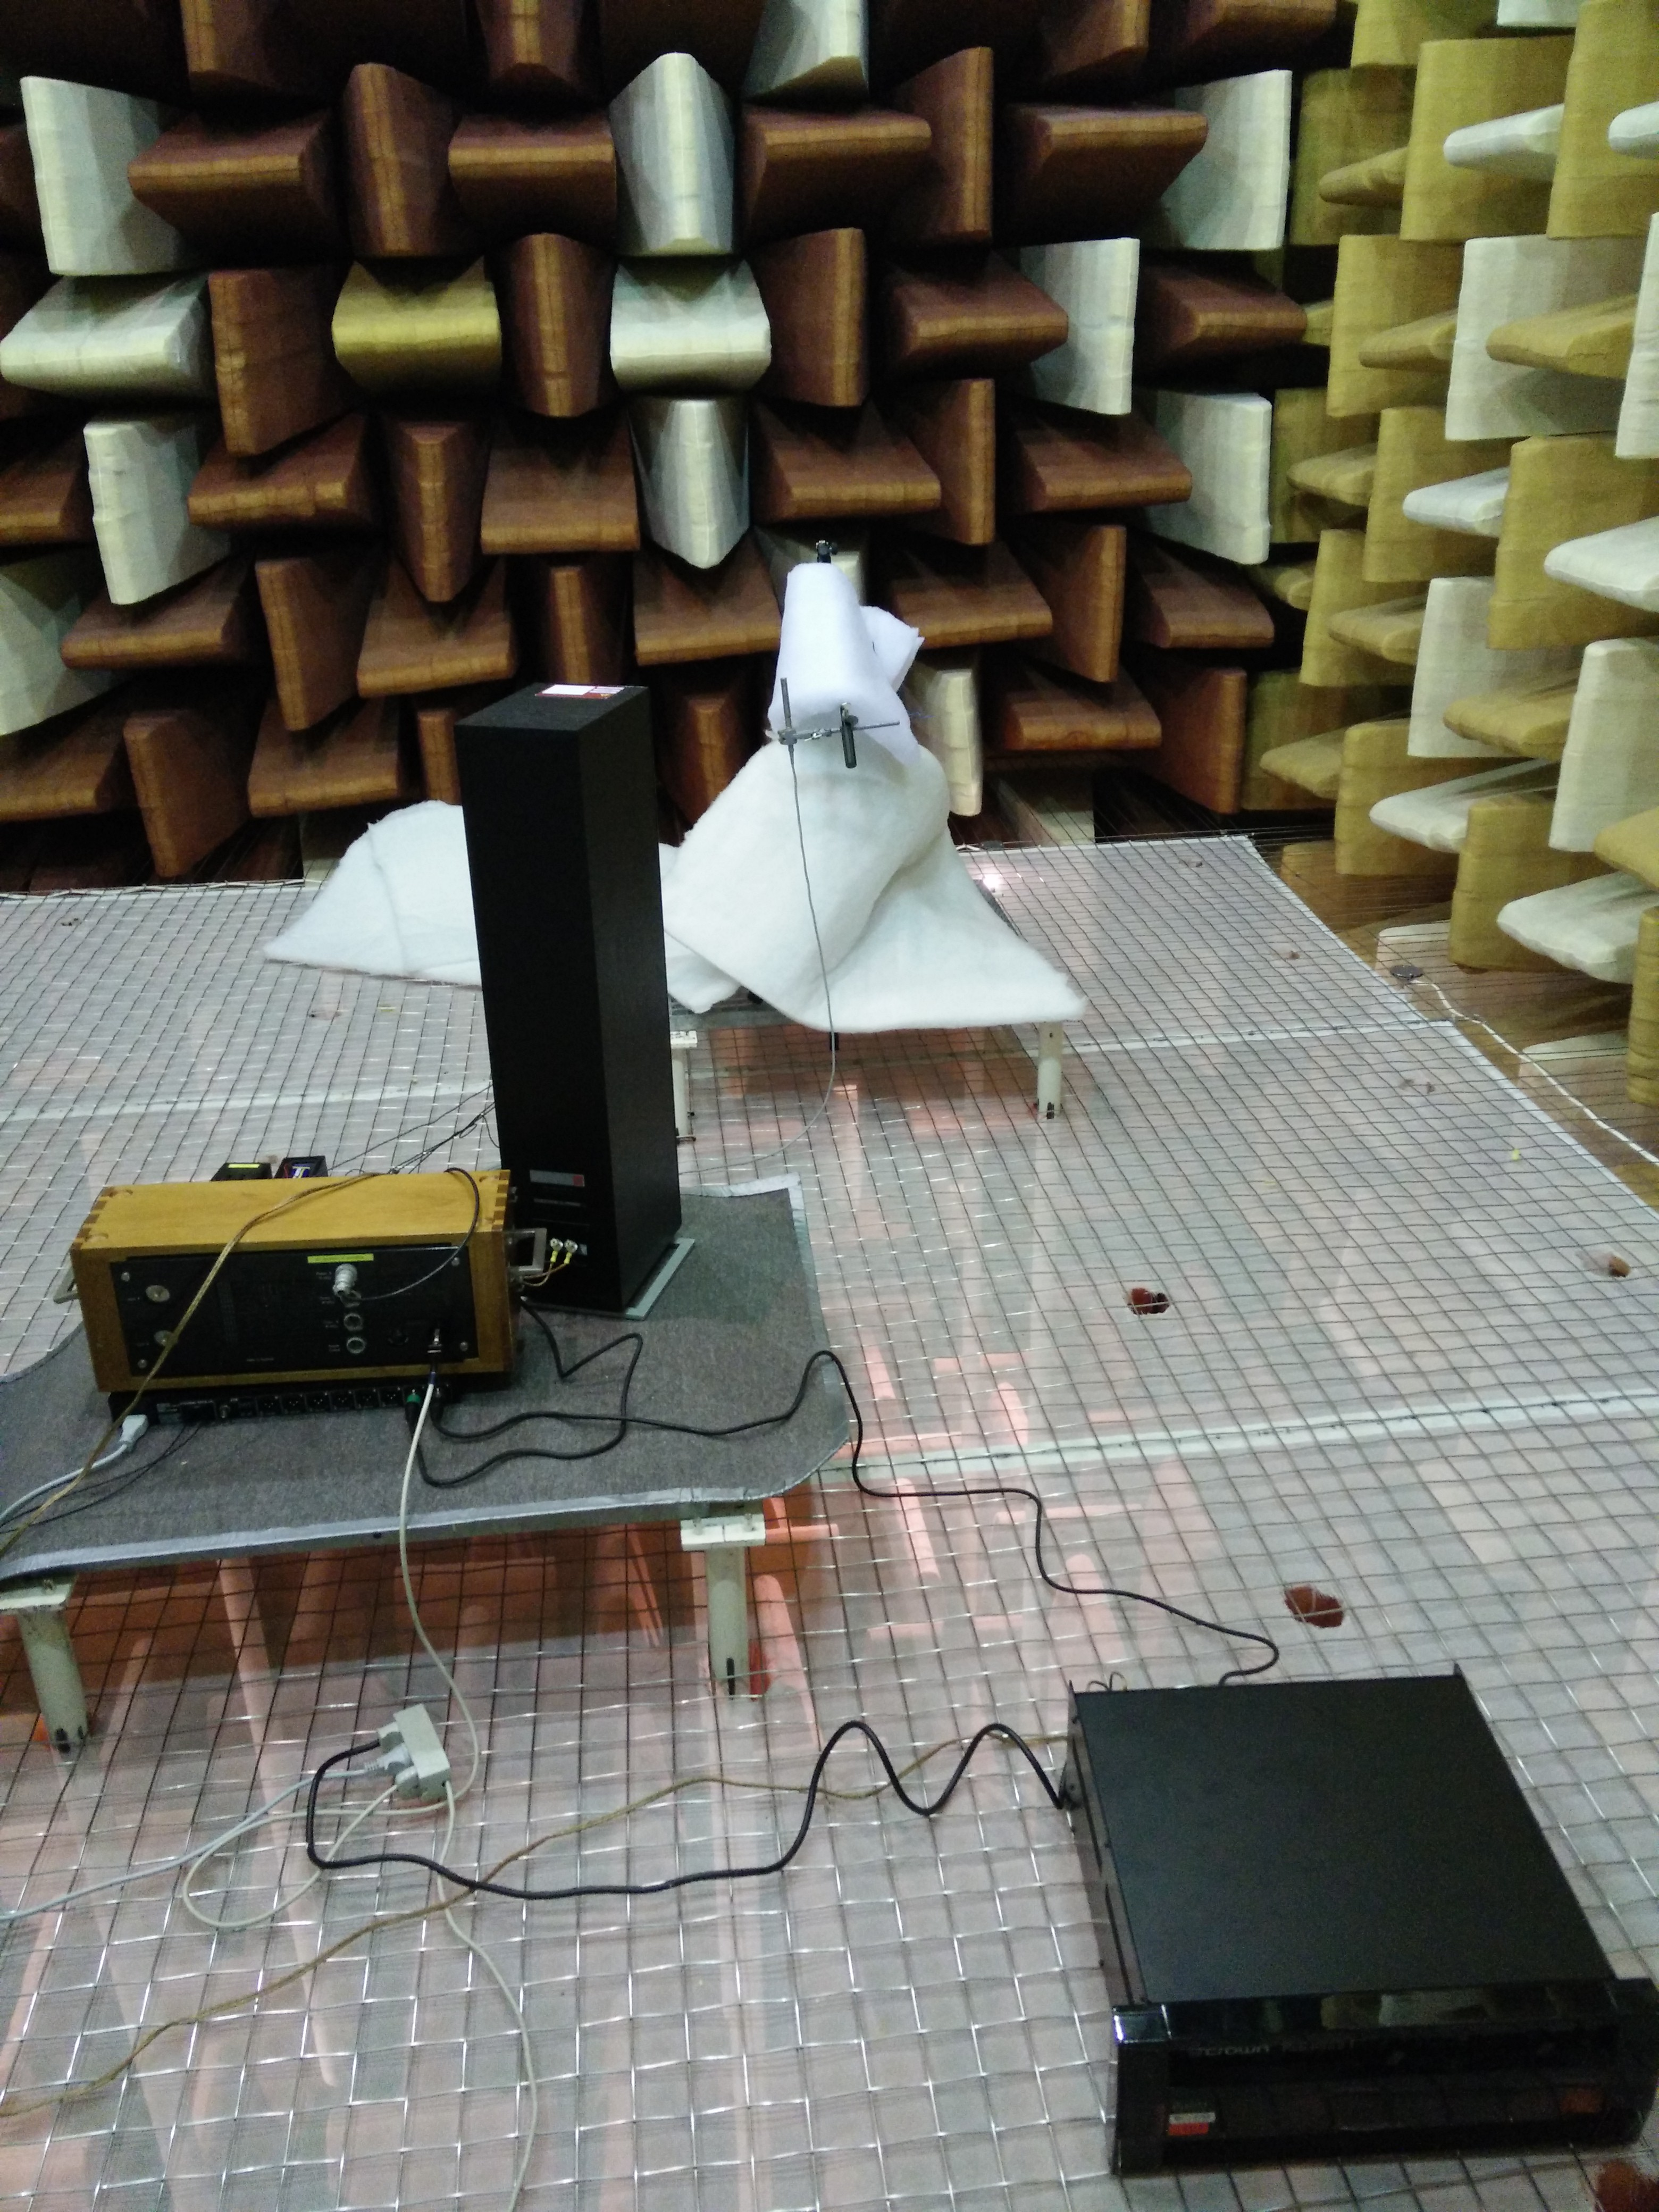
\includegraphics[width=1\textwidth]{figures/Test_setup_behind.jpg}
	\caption{Test setup (behind)}
	\label{fig:test_setup_behind_R}
\end{subfigure}
\hspace{6mm} 
\begin{subfigure}[t]{0.47\textwidth}
	\centering
	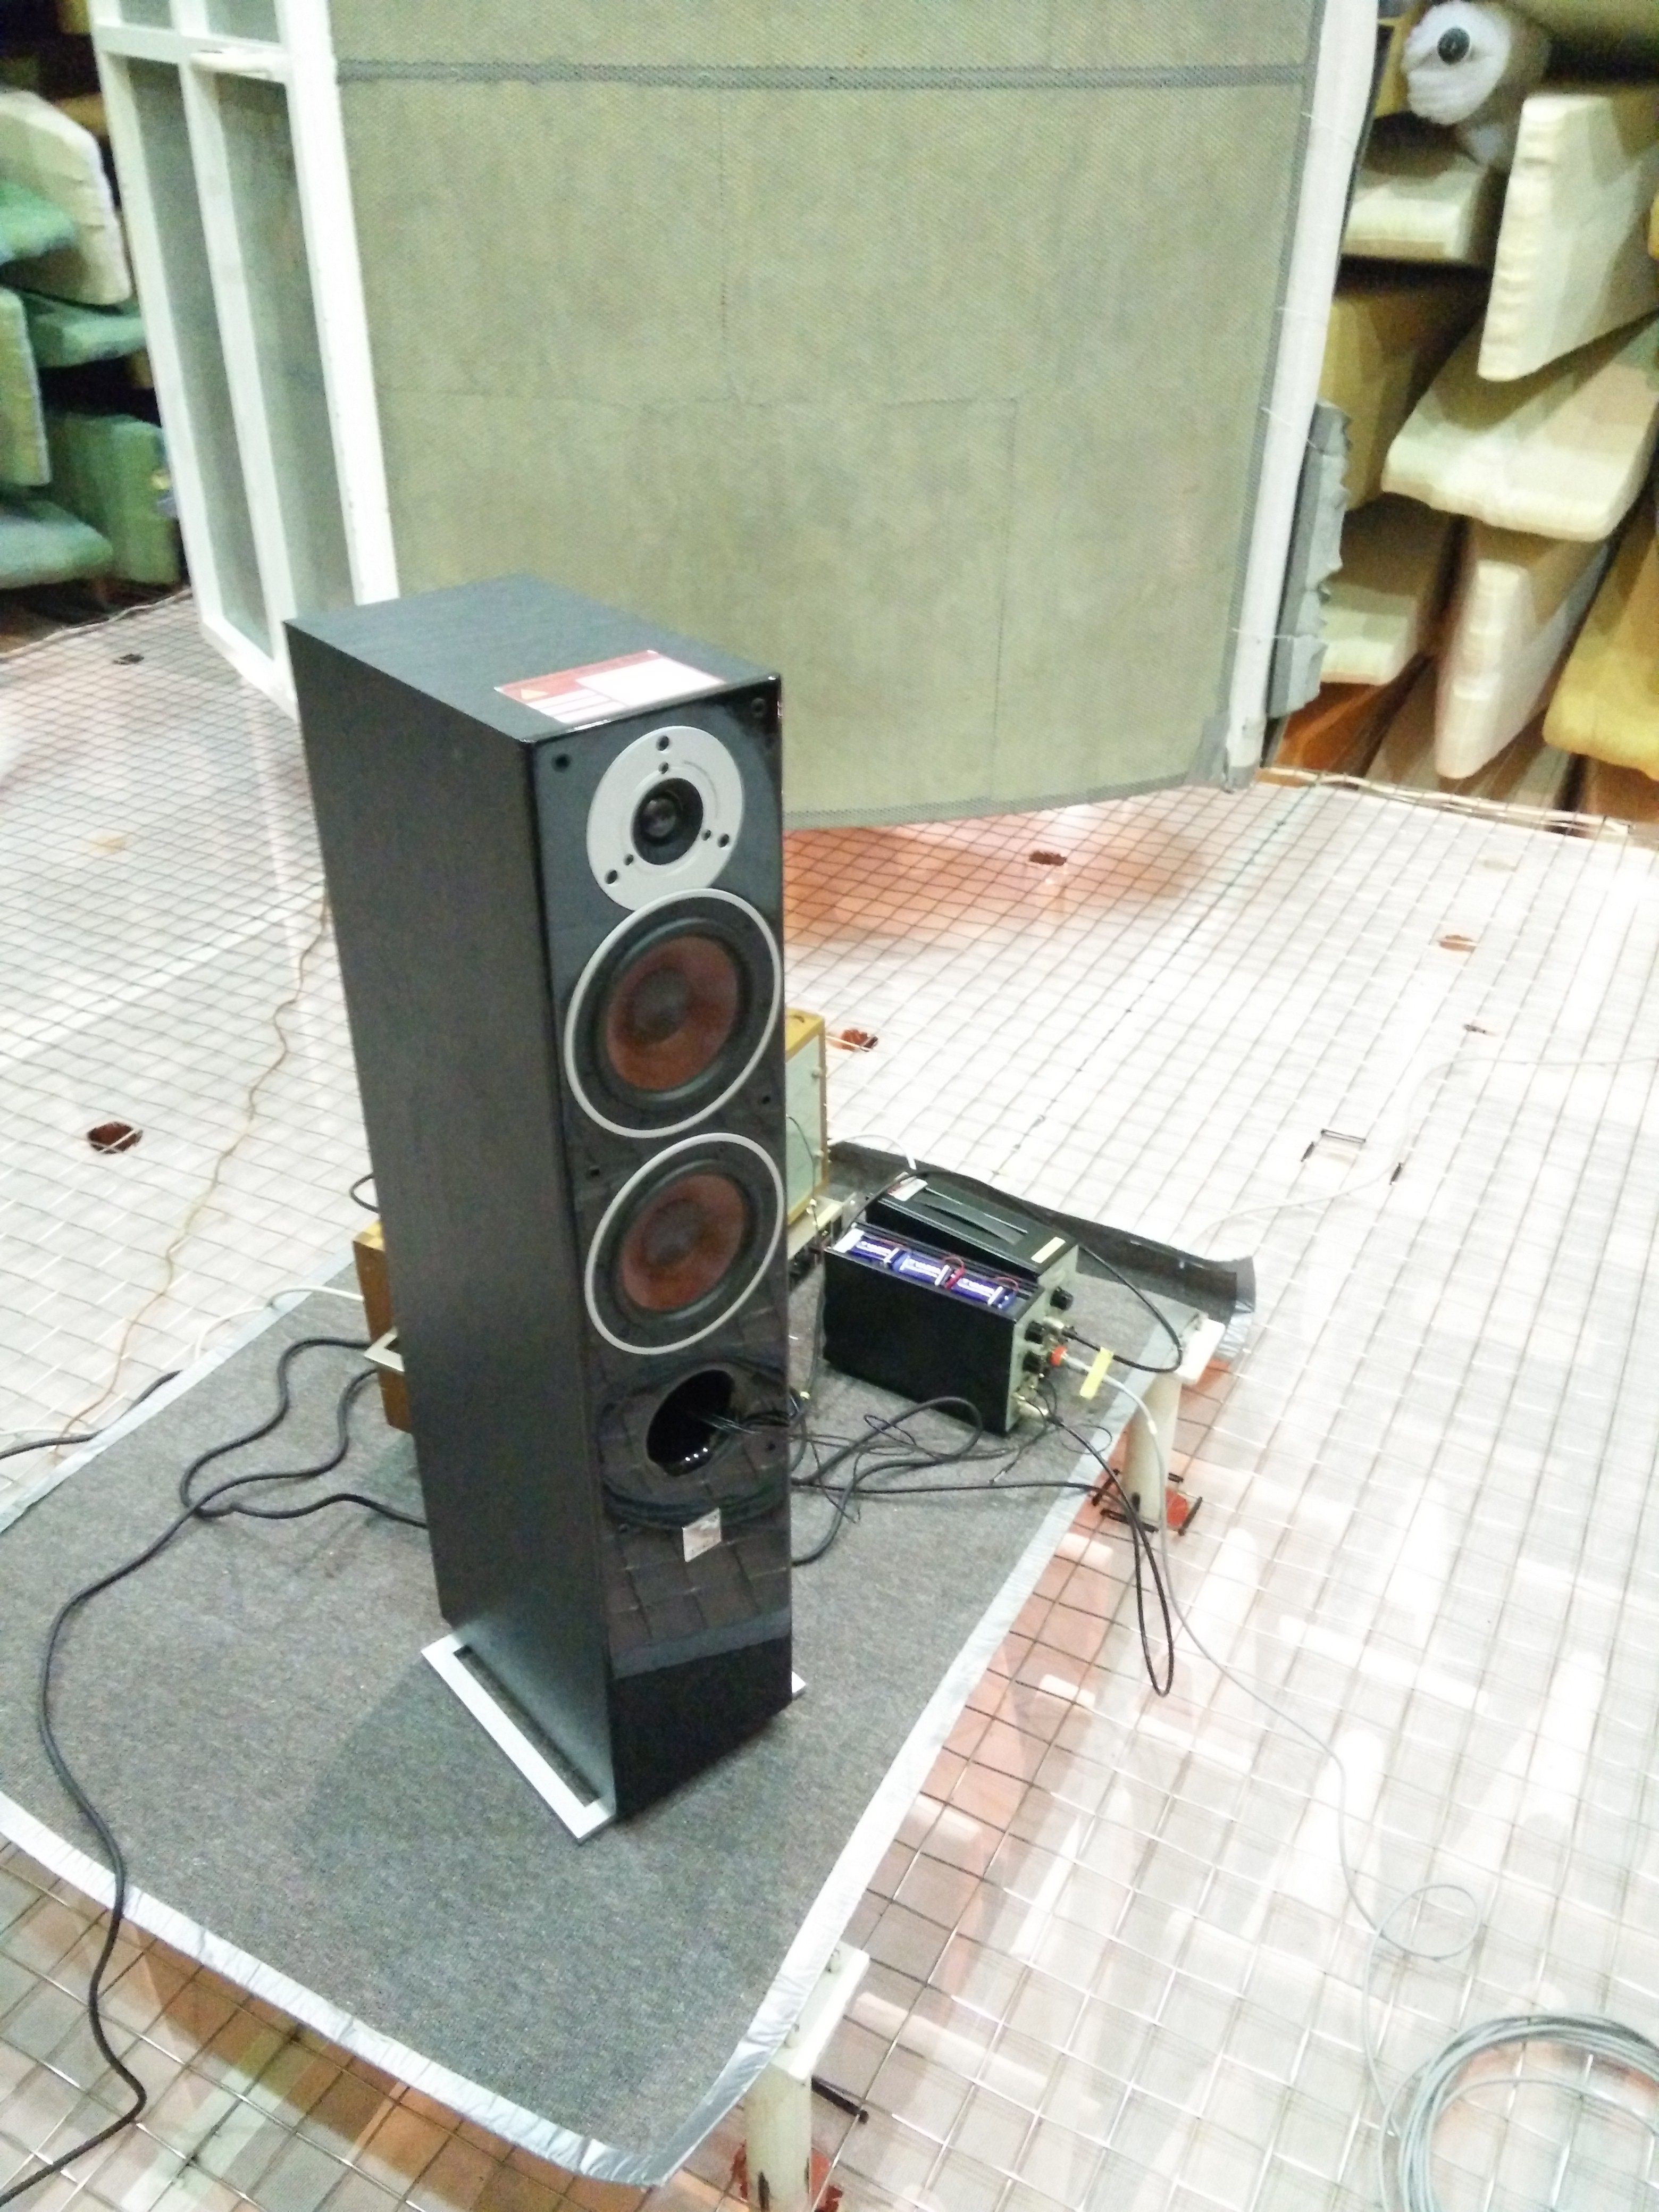
\includegraphics[width=1\textwidth]{figures/Test_setup_front.jpg}
	\caption{Test setup (front)}
	\label{fig:test_setup_front_R}
\end{subfigure}
\begin{subfigure}[b]{\textwidth}
	\centering
	\tikzsetnextfilename{TestSetup1}
	\begin{tikzpicture}
\node[input] (SpeakerCorner) at (0,0) {};
\node[PreAmpBox] (AMP0) at ($(6,-1.5)+(SpeakerCorner)$) {\scalebox{0.5}{Pre-amp}} ;
\node[PreAmpBox] (AMP1) at ($(0,-1)+(AMP0)$) {\scalebox{0.5}{Pre-amp}} ;
\node[PreAmpBox] (AMP2) at ($(0,-1)+(AMP1)$) {\scalebox{0.5}{Pre-amp}} ;
%\node[PreAmpBox] (AMP3) at ($(0,-1)+(AMP2)$) {\scalebox{0.5}{Pre-amp}} ;
%\node[PreAmpBox] (AMP4) at ($(0,-1)+(AMP3)$) {\scalebox{0.5}{Pre-amp}} ;
%\node[PreAmpBox] (AMP5) at ($(0,-1)+(AMP4)$) {\scalebox{0.5}{Pre-amp}} ;


%% Speaker Enclosure %%
%% Speaker %%
\draw[thick, fill=black!20] (SpeakerCorner) -- ($(2,0)+(SpeakerCorner)$) -- ($(2,-6)+(SpeakerCorner)$) -- ($(0,-6)+(SpeakerCorner)$) -- (SpeakerCorner);

\node[input] (Tweeter) at ($(0,-0.5)+(SpeakerCorner)$) {};
\draw[thick, fill=black!20] (Tweeter) -- ($(0,0.3)+(Tweeter)$) -- ($(0.5,0.25)+(Tweeter)$) -- ($(0.5,-0.25)+(Tweeter)$) -- ($(0,-0.3)+(Tweeter)$) -- (Tweeter);
\draw[thick, fill=black!20] ($(0.51,-0.25)+(Tweeter)$) -- ($(0.75,-0.25)+(Tweeter)$) -- ($(0.75,0.25)+(Tweeter)$) -- ($(0.51,0.25)+(Tweeter)$);

\node[input] (Speaker2) at ($(0,-2)+(SpeakerCorner)$) {};
\draw[thick, fill=black!20] (Speaker2) -- ($(0,0.5)+(Speaker2)$) -- ($(0.5,0.25)+(Speaker2)$) -- ($(0.5,-0.25)+(Speaker2)$) -- ($(0,-0.5)+(Speaker2)$) -- (Speaker2);
\draw[thick, fill=black!20] ($(0.51,-0.25)+(Speaker2)$) -- ($(0.75,-0.25)+(Speaker2)$) -- ($(0.75,0.25)+(Speaker2)$) -- ($(0.51,0.25)+(Speaker2)$);

\node[input] (Speaker) at ($(0,-3.5)+(SpeakerCorner)$) {};
\draw[thick, fill=black!20] (Speaker) -- ($(0,0.5)+(Speaker)$) -- ($(0.5,0.25)+(Speaker)$) -- ($(0.5,-0.25)+(Speaker)$) -- ($(0,-0.5)+(Speaker)$) -- (Speaker);
\draw[thick, fill=black!20] ($(0.51,-0.25)+(Speaker)$) -- ($(0.75,-0.25)+(Speaker)$) -- ($(0.75,0.25)+(Speaker)$) -- ($(0.51,0.25)+(Speaker)$);

\draw[thick, fill=black!20] ($(2,-5.5)+(SpeakerCorner)$) -- ($(1,-5.5)+(SpeakerCorner)$) -- ($(1,-5)+(SpeakerCorner)$) -- ($(2,-5)+(SpeakerCorner)$) -- ($(2,-5.5)+(SpeakerCorner)$);

%% Computer + AMP %%
\begin{pgfonlayer}{bg}
\node[input] (ComputerCorner) at (8,-1) {};
\draw[thick, fill=black!20] (ComputerCorner) -- ($(2,0)+(ComputerCorner)$) -- ($(2,-4)+(ComputerCorner)$) -- ($(0,-4)+(ComputerCorner)$) -- (ComputerCorner);
\end{pgfonlayer}{bg}

\node[] (Computer) at ($(1,-2)+(ComputerCorner)$) {ADC/DAC};

\node[PreAmpBox] (AMP) at ($(1,-5)+(ComputerCorner)$) {\scalebox{0.5}{Amplifier}} ;

%% Draw Lines %%

%% Pre-amp to Speaker
\draw[<-,mark=*] (AMP0) -- ($(-3,0)+(AMP0)$) |- ($(-1.5,0.5)+(SpeakerCorner)$) -- ($(-1.5,-2)+(SpeakerCorner)$) ;
\draw [red,fill] ($(-1.5,-2)+(SpeakerCorner)$) circle [radius=0.1];

\draw[<-,mark=*] (AMP1) -| ($(-4.25,1.5)+(AMP1)$) ;
\draw [blue,fill] ($(-4.25,1.5)+(AMP1)$) circle [radius=0.1];

\draw[<-,mark=*] (AMP2) -- ($(-5.25,-0)+(AMP2)$) ;
\draw [blue,fill] ($(-5.25,-0)+(AMP2)$) circle [radius=0.1];

%\draw[<-,mark=*] (AMP3) -- ($(-5.5,0)+(AMP3)$) ;
%\draw [blue,fill] ($(-5.5,0)+(AMP3)$) circle [radius=0.1];

%\draw[<-,mark=*] (AMP4) -- ($(-4.5,0)+(AMP4)$) ;
%\draw [blue,fill] ($(-4.5,0)+(AMP4)$) circle [radius=0.1];

%\draw[<-,mark=*] (AMP5) -| ($(-3.5,0.25)+(AMP5)$) -| ($(1.5,-5.25)+(SpeakerCorner)$) ;
%\draw [blue,fill] ($(1.5,-5.25)+(SpeakerCorner)$) circle [radius=0.1];

\draw[->,mark=*] (AMP) -| ($(2.25,-5.75)+(SpeakerCorner)$) |- ($(2,-5.4)+(SpeakerCorner)$) ;

%% Amps to Computer

\draw[<-,mark=*] (AMP) -- ($(1,-4)+(ComputerCorner)$) ;
\draw[->] (AMP0) -| ($(-0.5,-0.5)+(ComputerCorner)$) -- ($(0,-0.5)+(ComputerCorner)$) ;
\draw[->] (AMP1) -- ($(0,-1.5)+(ComputerCorner)$) ;
\draw[->] (AMP2) -- ($(0,-2.5)+(ComputerCorner)$) ;
%\draw[->] (AMP3) -| ($(-0.75,-2)+(ComputerCorner)$)  -- ($(0,-2)+(ComputerCorner)$) ;
%\draw[->] (AMP4) -| ($(-0.75,-3)+(ComputerCorner)$)  -- ($(0,-3)+(ComputerCorner)$) ;
%\draw[->] (AMP5) -| ($(-0.75,-3.75)+(ComputerCorner)$)  -- ($(0,-3.75)+(ComputerCorner)$) ;
%\draw[->] (AMP5) -| ($(-0.75,-3.75)+(ComputerCorner)$)  -- ($(0,-3.75)+(ComputerCorner)$) ;
%\draw[->] (AMP5) -| ($(-0.75,-3.75)+(ComputerCorner)$)  -- ($(0,-3.75)+(ComputerCorner)$) ;
%% Rooms

\draw[->] ($(0,0.75)+(AMP)$) -- ($(-2,0.75)+(AMP)$) -- ($(-2,1.25)+(AMP)$) -- ($(-1,1.25)+(AMP)$);

\draw[thick, dashed] ($(-2,1)+(SpeakerCorner)$) -- ($(10.5,1)+(SpeakerCorner)$) -- ($(10.5,-7)+(SpeakerCorner)$) -- ($(-2,-7)+(SpeakerCorner)$) -- ($(-2,1)+(SpeakerCorner)$);
\draw node [black, above=0.05] at ($(-0.25,-7)+(SpeakerCorner)$) {Anechoic room};


%% To Computer %%
\begin{pgfonlayer}{bg}
\node[input] (PC) at (13,-1) {};
\draw[thick, fill=black!20] (PC) -- ($(2,0)+(PC)$) -- ($(2,-2)+(PC)$) -- ($(0,-2)+(PC)$) -- (PC);
\end{pgfonlayer}{bg}


\draw[<->] ($(-3,-1)+(PC)$) -- node[above] {SPDIF} ($(0,-1)+(PC)$) ;
\node[] (PC1) at ($(1,-1)+(PC)$) {Computer};

\end{tikzpicture}
	\caption{Schematic overview}
	\label{figure:SpeakertestSetup}
\end{subfigure}
\caption{The entire test setup shown with photographs and a schematic overview}
\label{fig:test_setup_R}
\end{figure}


\subsection*{Equipment used and AAU-no.}

\begin{table}[H]
\centering
\ra{1.3}
\begin{tabular}{S[table-format=1]ccc} \toprule
    {Item} & {Description} & {AAU-no} \\ \bottomrule 
    1      &  B \& K Accelerometer Type 4319  & 06598   \\ 
    2      &  B \& K Accelerometer Type 4333  & 06596   \\ 
    3      &  B \& K 2-channel Accelerometer Pre-amp Type 2622  & 07013   \\
    4      &  B \& K Microphone Type 4165  & 08132   \\
    5      &  Gras - 26AK Pre-amp & 52665   \\
    6      &  B \& K Microphone Power supply Type 2804  & 07304   \\
    7      &  Crown Studio Reference I Amplifier & 52614   \\
    8      &  BEHRINGER digital A/D \& D/A Converter - Model ADA8000   & 56545   \\
    9      &  B \& K Accelerometer calibrator 4294 & 08023   \\
    10     &  B \& K Microphone calibrator 4231 & 78301   \\
    11     &  RME HammerFall DIGI 96-PDST sound card & 60919  \\
    11     &  Passive Dali Zensor 5 AX & NaN  \\ \bottomrule 
\end{tabular}
\caption{Table over equipment used in the test}
\label{tab:UsedEquipment1}
\end{table}
\vspace{-5mm}


\section{Procedure}\label{sec:SpeakerTestProcedure1}

The producer for this experiment is described as follows:
\vspace{-5mm}
\begin{enumerate}
\item Adjust volume on the amplifier to +3 dB gain.
\item Vacate the anechoic room and seal the room.
\item Start recording in Adobe Audition for:
\begin{itemize}
\item Driver and enclosure accelerometer
\item Microphone and playback loop
\end{itemize}
\item Playback file \path{chirp.wav}, which is a sinusoidal sweep from 2.4 kHz to 10 Hz. The duration of the sweep is 30 seconds and the sweep is linear. The amplitude is 0 dBFS.
\item After playback, stop recording all channels
\item Save recordings as \path{.wav} file
\item Enter room and adjust amplifier by +1 dB
\item Repeat step 2 through 7 until the speaker breaks.
\end{enumerate}

The \path{chirp.wav} are located at:\\
\scalebox{0.7}{
\path{CD://Maalinger/Maalinger030316 - Loudspeaker test/Measurements030316/chirp.wav}}\\


%\begin{figure}[H]
%\centering
%\tikzsetnextfilename{linear_freq_sweep}
%% This file was created by matlab2tikz.
%
%The latest updates can be retrieved from
%  http://www.mathworks.com/matlabcentral/fileexchange/22022-matlab2tikz-matlab2tikz
%where you can also make suggestions and rate matlab2tikz.
%
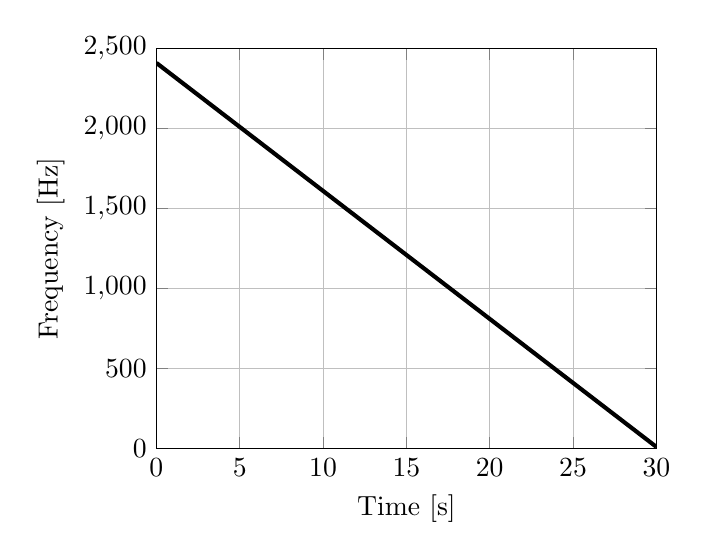
\begin{tikzpicture}

\begin{axis}[%
width=2.5in,
height=2in,
at={(1.011in,0.642in)},
scale only axis,
xmin=0,
xmax=30,
xmajorgrids,
ymin=0,
ymax=2500,
ymajorgrids,
xlabel={Time [s]},
ylabel={Frequency [Hz]},
axis background/.style={fill=white}
]
\addplot [color=black,solid,line width=1.5pt,forget plot]
  table[row sep=crcr]{%
0	2410\\
0.1	2402\\
0.2	2394\\
0.3	2386\\
0.4	2378\\
0.5	2370\\
0.6	2362\\
0.7	2354\\
0.8	2346\\
0.9	2338\\
1	2330\\
1.1	2322\\
1.2	2314\\
1.3	2306\\
1.4	2298\\
1.5	2290\\
1.6	2282\\
1.7	2274\\
1.8	2266\\
1.9	2258\\
2	2250\\
2.1	2242\\
2.2	2234\\
2.3	2226\\
2.4	2218\\
2.5	2210\\
2.6	2202\\
2.7	2194\\
2.8	2186\\
2.9	2178\\
3	2170\\
3.1	2162\\
3.2	2154\\
3.3	2146\\
3.4	2138\\
3.5	2130\\
3.6	2122\\
3.7	2114\\
3.8	2106\\
3.9	2098\\
4	2090\\
4.1	2082\\
4.2	2074\\
4.3	2066\\
4.4	2058\\
4.5	2050\\
4.6	2042\\
4.7	2034\\
4.8	2026\\
4.9	2018\\
5	2010\\
5.1	2002\\
5.2	1994\\
5.3	1986\\
5.4	1978\\
5.5	1970\\
5.6	1962\\
5.7	1954\\
5.8	1946\\
5.9	1938\\
6	1930\\
6.1	1922\\
6.2	1914\\
6.3	1906\\
6.4	1898\\
6.5	1890\\
6.6	1882\\
6.7	1874\\
6.8	1866\\
6.9	1858\\
7	1850\\
7.1	1842\\
7.2	1834\\
7.3	1826\\
7.4	1818\\
7.5	1810\\
7.6	1802\\
7.7	1794\\
7.8	1786\\
7.9	1778\\
8	1770\\
8.1	1762\\
8.2	1754\\
8.3	1746\\
8.4	1738\\
8.5	1730\\
8.6	1722\\
8.7	1714\\
8.8	1706\\
8.9	1698\\
9	1690\\
9.1	1682\\
9.2	1674\\
9.3	1666\\
9.4	1658\\
9.5	1650\\
9.6	1642\\
9.7	1634\\
9.8	1626\\
9.9	1618\\
10	1610\\
10.1	1602\\
10.2	1594\\
10.3	1586\\
10.4	1578\\
10.5	1570\\
10.6	1562\\
10.7	1554\\
10.8	1546\\
10.9	1538\\
11	1530\\
11.1	1522\\
11.2	1514\\
11.3	1506\\
11.4	1498\\
11.5	1490\\
11.6	1482\\
11.7	1474\\
11.8	1466\\
11.9	1458\\
12	1450\\
12.1	1442\\
12.2	1434\\
12.3	1426\\
12.4	1418\\
12.5	1410\\
12.6	1402\\
12.7	1394\\
12.8	1386\\
12.9	1378\\
13	1370\\
13.1	1362\\
13.2	1354\\
13.3	1346\\
13.4	1338\\
13.5	1330\\
13.6	1322\\
13.7	1314\\
13.8	1306\\
13.9	1298\\
14	1290\\
14.1	1282\\
14.2	1274\\
14.3	1266\\
14.4	1258\\
14.5	1250\\
14.6	1242\\
14.7	1234\\
14.8	1226\\
14.9	1218\\
15	1210\\
15.1	1202\\
15.2	1194\\
15.3	1186\\
15.4	1178\\
15.5	1170\\
15.6	1162\\
15.7	1154\\
15.8	1146\\
15.9	1138\\
16	1130\\
16.1	1122\\
16.2	1114\\
16.3	1106\\
16.4	1098\\
16.5	1090\\
16.6	1082\\
16.7	1074\\
16.8	1066\\
16.9	1058\\
17	1050\\
17.1	1042\\
17.2	1034\\
17.3	1026\\
17.4	1018\\
17.5	1010\\
17.6	1002\\
17.7	994\\
17.8	986\\
17.9	978\\
18	970\\
18.1	962\\
18.2	954\\
18.3	946\\
18.4	938\\
18.5	930\\
18.6	922\\
18.7	914\\
18.8	906\\
18.9	898\\
19	890\\
19.1	882\\
19.2	874\\
19.3	866\\
19.4	858\\
19.5	850\\
19.6	842\\
19.7	834\\
19.8	826\\
19.9	818\\
20	810\\
20.1	802\\
20.2	794\\
20.3	786\\
20.4	778\\
20.5	770\\
20.6	762\\
20.7	754\\
20.8	746\\
20.9	738\\
21	730\\
21.1	722\\
21.2	714\\
21.3	706\\
21.4	698\\
21.5	690\\
21.6	682\\
21.7	674\\
21.8	666\\
21.9	658\\
22	650\\
22.1	642\\
22.2	634\\
22.3	626\\
22.4	618\\
22.5	610\\
22.6	602\\
22.7	594\\
22.8	586\\
22.9	578\\
23	570\\
23.1	562\\
23.2	554\\
23.3	546\\
23.4	538\\
23.5	530\\
23.6	522\\
23.7	514\\
23.8	506\\
23.9	498\\
24	490\\
24.1	482\\
24.2	474\\
24.3	466\\
24.4	458\\
24.5	450\\
24.6	442\\
24.7	434\\
24.8	426\\
24.9	418\\
25	410\\
25.1	402\\
25.2	394\\
25.3	386\\
25.4	378\\
25.5	370\\
25.6	362\\
25.7	354\\
25.8	346\\
25.9	338\\
26	330\\
26.1	322\\
26.2	314\\
26.3	306\\
26.4	298\\
26.5	290\\
26.6	282\\
26.7	274\\
26.8	266\\
26.9	258\\
27	250\\
27.1	242\\
27.2	234\\
27.3	226\\
27.4	218\\
27.5	210\\
27.6	202\\
27.7	194\\
27.8	186\\
27.9	178\\
28	170\\
28.1	162\\
28.2	154\\
28.3	146\\
28.4	138\\
28.5	130\\
28.6	122\\
28.7	114\\
28.8	106\\
28.9	98\\
29	90\\
29.1	82\\
29.2	74\\
29.3	66\\
29.4	58\\
29.5	50\\
29.6	42\\
29.7	34\\
29.8	26\\
29.9	18\\
30	10\\
};
\end{axis}
\end{tikzpicture}%
%\caption{}
%\label{fig:linear_freq_sweep}
%\end{figure}



\section{Data Extraction}


It was possible to increase the volume by 19 dB until the loudspeaker unit got to damaged. The gain was linear increased by 1 dB, starting at 3 dB, until the 20th test were the loudspeaker unit failed. This results in 20 usable data sets.

The recordings can be found on:\\
\scalebox{0.7}{
\path{CD://Maalinger/Maalinger030316 - Loudspeaker test/Measurements030316/}}
And is indexed in folders \scalebox{0.8}{\path{Measure_X}}, where X corresponds to the test number. Every measurements inside is denoted as:
\begin{itemize}
\item Accelerometer on driver: \scalebox{0.8}{\path{Acc driver_0XX}}
\item Accelerometer in enclosure: \scalebox{0.8}{\path{Acc enclosure_0XX}}
\item Microphone: \scalebox{0.8}{\path{Mic_0XX}}
\item Playback loop: \scalebox{0.8}{\path{Reference_0XX}}
\end{itemize}

The Script used to create all graphs are located at:\\
\scalebox{0.7}{
\path{CD://Maalinger/Maalinger030316 - Loudspeaker test/Measurements030316/MeasurementAnalysis.m}}\\
Figures used in the following \ref{subsec:Raw_data_1} and Dataset 1 though 20 can be found compiled in a combined file at:
\scalebox{0.7}{
\path{CD://Maalinger/Maalinger030316 - Loudspeaker test/Measurements030316/AlleSamlet.pdf}}


\subsection{Raw Data}\label{subsec:Raw_data_1}

For each of the test four measurements was taken. These are the accelerometer placed on the driver and enclosure, the microphone and a reference to synchronize the measurements. 

As previously stated there are in total 20 datasets each containing four measurements, namely the vibrations from the enclosure and driver, the sound pressure from the microphone, and lastly a reference signal to synchronize all data. The amount of data is therefore large and only relevant datasets will be presented. The first dataset from the test is shown in \autoref{fig:raw1}.


\begin{figure}[H]
\centering
\begin{subfigure}[t]{0.335\textwidth}
	\tikzsetnextfilename{Raw_Driver1}
	% This file was created by matlab2tikz.
%
%The latest updates can be retrieved from
%  http://www.mathworks.com/matlabcentral/fileexchange/22022-matlab2tikz-matlab2tikz
%where you can also make suggestions and rate matlab2tikz.
%
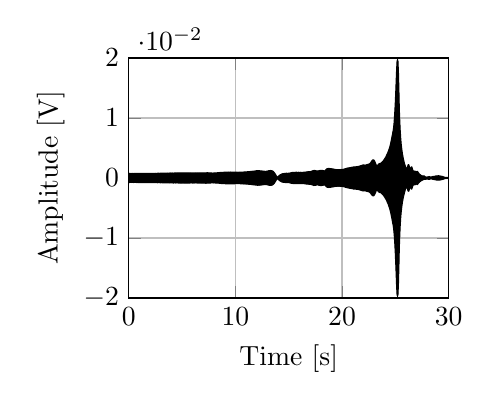
\begin{tikzpicture}

\begin{axis}[%
width=1.6in,
height=1.2in,
at={(0.758in,0.481in)},
scale only axis,
xmin=0,
xmax=30,
xmajorgrids,
ymin=-0.02,
ymax=0.02,
ymajorgrids,
xlabel={Time [s]},
ylabel={Amplitude [V]},
axis background/.style={fill=white}
]
\addplot[fill=black,draw=black,forget plot] plot table[row sep=crcr]{%
2.08333333333333e-05	0.000842452049255371\\
0.0417454218822439	0.000724315643310547\\
0.0834700104311544	0.000728130340576172\\
0.125194598980065	0.000715255737304688\\
0.166919187528975	0.000736355781555176\\
0.208643776077886	0.000741124153137207\\
0.250368364626797	0.000725150108337402\\
0.292092953175707	0.00073695182800293\\
0.333817541724618	0.000734806060791016\\
0.375542130273528	0.000743985176086426\\
0.417266718822439	0.000729680061340332\\
0.458991307371349	0.00072777271270752\\
0.50071589592026	0.000744819641113281\\
0.54244048446917	0.000737667083740234\\
0.584165073018081	0.000739336013793945\\
0.625889661566991	0.000748038291931152\\
0.667614250115902	0.000733852386474609\\
0.709338838664812	0.000737309455871582\\
0.751063427213723	0.00073850154876709\\
0.792788015762633	0.000756502151489258\\
0.834512604311544	0.000747323036193848\\
0.876237192860454	0.000743627548217773\\
0.917961781409365	0.000749349594116211\\
0.959686369958275	0.000751495361328125\\
1.00141095850719	0.000746369361877441\\
1.0431355470561	0.000753998756408691\\
1.08486013560501	0.000748515129089355\\
1.12658472415392	0.00075221061706543\\
1.16830931270283	0.000759720802307129\\
1.21003390125174	0.000748515129089355\\
1.25175848980065	0.000764369964599609\\
1.29348307834956	0.000760555267333984\\
1.33520766689847	0.000766396522521973\\
1.37693225544738	0.000762343406677246\\
1.41865684399629	0.000754714012145996\\
1.4603814325452	0.000761151313781738\\
1.50210602109411	0.000756978988647461\\
1.54383060964302	0.000756144523620605\\
1.58555519819193	0.000763535499572754\\
1.62727978674084	0.000756502151489258\\
1.66900437528975	0.000757694244384766\\
1.71072896383866	0.000751137733459473\\
1.75245355238758	0.000756502151489258\\
1.79417814093649	0.000756144523620605\\
1.8359027294854	0.000758051872253418\\
1.87762731803431	0.00075685977935791\\
1.91935190658322	0.000754356384277344\\
1.96107649513213	0.000756144523620605\\
2.00280108368104	0.000751018524169922\\
2.04452567222995	0.000769376754760742\\
2.08625026077886	0.000757336616516113\\
2.12797484932777	0.000759363174438477\\
2.16969943787668	0.000766515731811523\\
2.21142402642559	0.00075685977935791\\
2.2531486149745	0.000760316848754883\\
2.29487320352341	0.000762820243835449\\
2.33659779207232	0.000757813453674316\\
2.37832238062123	0.000756382942199707\\
2.42004696917014	0.000770211219787598\\
2.46177155771905	0.00077366828918457\\
2.50349614626796	0.000762701034545898\\
2.54522073481687	0.000776529312133789\\
2.58694532336579	0.000768661499023438\\
2.6286699119147	0.000769495964050293\\
2.67039450046361	0.000769376754760742\\
2.71211908901252	0.000779390335083008\\
2.75384367756143	0.000778675079345703\\
2.79556826611034	0.000775575637817383\\
2.83729285465925	0.0007781982421875\\
2.87901744320816	0.00077354907989502\\
2.92074203175707	0.000772714614868164\\
2.96246662030598	0.000776886940002441\\
3.00419120885489	0.000785589218139648\\
3.0459157974038	0.000795722007751465\\
3.08764038595271	0.000782370567321777\\
3.12936497450162	0.00078272819519043\\
3.17108956305053	0.000790238380432129\\
3.21281415159944	0.00079810619354248\\
3.25453874014835	0.000793933868408203\\
3.29626332869726	0.000802278518676758\\
3.33798791724618	0.000802397727966309\\
3.37971250579509	0.00080108642578125\\
3.421437094344	0.000811576843261719\\
3.46316168289291	0.000808596611022949\\
3.50488627144182	0.000804781913757324\\
3.54661085999073	0.000814437866210938\\
3.58833544853964	0.000810384750366211\\
3.63006003708855	0.000816583633422852\\
3.67178462563746	0.000807762145996094\\
3.71350921418637	0.000812888145446777\\
3.75523380273528	0.000812768936157227\\
3.79695839128419	0.000815749168395996\\
3.8386829798331	0.000813961029052734\\
3.88040756838201	0.000826478004455566\\
3.92213215693092	0.000814437866210938\\
3.96385674547983	0.000813722610473633\\
4.00558133402874	0.000811934471130371\\
4.04730592257765	0.000820755958557129\\
4.08903051112656	0.000818610191345215\\
4.13075509967547	0.000812888145446777\\
4.17247968822439	0.000814914703369141\\
4.2142042767733	0.000813126564025879\\
4.25592886532221	0.000823259353637695\\
4.29765345387112	0.000821471214294434\\
4.33937804242003	0.000811576843261719\\
4.38110263096894	0.000824570655822754\\
4.42282721951785	0.000835657119750977\\
4.46455180806676	0.000819563865661621\\
4.50627639661567	0.000821113586425781\\
4.54800098516458	0.000826597213745117\\
4.58972557371349	0.000843286514282227\\
4.6314501622624	0.00083458423614502\\
4.67317475081131	0.000841140747070313\\
4.71489933936022	0.000822782516479492\\
4.75662392790913	0.00083160400390625\\
4.79834851645804	0.000840425491333008\\
4.84007310500695	0.000842809677124023\\
4.88179769355586	0.000837802886962891\\
4.92352228210478	0.000848293304443359\\
4.96524687065368	0.000842094421386719\\
5.0069714592026	0.000839948654174805\\
5.04869604775151	0.000844120979309082\\
5.09042063630042	0.000840306282043457\\
5.13214522484933	0.000838994979858398\\
5.17386981339824	0.000844478607177734\\
5.21559440194715	0.000845789909362793\\
5.25731899049606	0.000832080841064453\\
5.29904357904497	0.000855803489685059\\
5.34076816759388	0.000848174095153809\\
5.38249275614279	0.000844120979309082\\
5.4242173446917	0.000833272933959961\\
5.46594193324061	0.000838756561279297\\
5.50766652178952	0.000839591026306152\\
5.54939111033843	0.000842094421386719\\
5.59111569888734	0.000841498374938965\\
5.63284028743625	0.000836610794067383\\
5.67456487598516	0.000829100608825684\\
5.71628946453407	0.000816583633422852\\
5.75801405308299	0.000837326049804688\\
5.7997386416319	0.000834465026855469\\
5.84146323018081	0.000824809074401855\\
5.88318781872972	0.000816226005554199\\
5.92491240727863	0.000822067260742188\\
5.96663699582754	0.000817298889160156\\
6.00836158437645	0.000820398330688477\\
6.05008617292536	0.000815391540527344\\
6.09181076147427	0.000821232795715332\\
6.13353535002318	0.000823259353637695\\
6.17525993857209	0.000811100006103516\\
6.216984527121	0.000824093818664551\\
6.25870911566991	0.00082862377166748\\
6.30043370421882	0.00082707405090332\\
6.34215829276773	0.000818133354187012\\
6.38388288131664	0.00082695484161377\\
6.42560746986555	0.000823736190795898\\
6.46733205841446	0.000827789306640625\\
6.50905664696338	0.000817418098449707\\
6.55078123551229	0.00083315372467041\\
6.5925058240612	0.00083458423614502\\
6.63423041261011	0.000834822654724121\\
6.67595500115902	0.000837922096252441\\
6.71767958970793	0.000827908515930176\\
6.75940417825684	0.00082862377166748\\
6.80112876680575	0.000835776329040527\\
6.84285335535466	0.000834941864013672\\
6.88457794390357	0.000837326049804688\\
6.92630253245248	0.000839829444885254\\
6.96802712100139	0.000847339630126953\\
7.0097517095503	0.00084376335144043\\
7.05147629809921	0.000843644142150879\\
7.09320088664812	0.000847101211547852\\
7.13492547519703	0.000847339630126953\\
7.17665006374594	0.000843644142150879\\
7.21837465229485	0.000848174095153809\\
7.26009924084376	0.000854969024658203\\
7.30182382939268	0.000855684280395508\\
7.34354841794159	0.000865817070007324\\
7.3852730064905	0.000864505767822266\\
7.42699759503941	0.000867962837219238\\
7.46872218358832	0.000847101211547852\\
7.51044677213723	0.000849604606628418\\
7.55217136068614	0.000842928886413574\\
7.59389594923505	0.000854134559631348\\
7.63562053778396	0.000830292701721191\\
7.67734512633287	0.000824570655822754\\
7.71906971488178	0.000828742980957031\\
7.76079430343069	0.000830650329589844\\
7.8025188919796	0.000817418098449707\\
7.84424348052851	0.00081479549407959\\
7.88596806907742	0.000807404518127441\\
7.92769265762633	0.000814914703369141\\
7.96941724617524	0.000820755958557129\\
8.01114183472416	0.000833749771118164\\
8.05286642327307	0.000829458236694336\\
8.09459101182198	0.000839948654174805\\
8.13631560037089	0.00084376335144043\\
8.1780401889198	0.000843167304992676\\
8.21976477746871	0.000849008560180664\\
8.26148936601762	0.000846505165100098\\
8.30321395456653	0.000858187675476074\\
8.34493854311544	0.000867486000061035\\
8.38666313166435	0.000872135162353516\\
8.42838772021326	0.000874876976013184\\
8.47011230876217	0.000872969627380371\\
8.51183689731108	0.000886321067810059\\
8.55356148585999	0.00090634822845459\\
8.5952860744089	0.000900864601135254\\
8.63701066295781	0.000904202461242676\\
8.67873525150672	0.000906229019165039\\
8.72045984005563	0.000902056694030762\\
8.76218442860454	0.000916242599487305\\
8.80390901715345	0.000928282737731934\\
8.84563360570237	0.000935554504394531\\
8.88735819425128	0.000940561294555664\\
8.92908278280018	0.000948786735534668\\
8.9708073713491	0.000948309898376465\\
9.01253195989801	0.000955462455749512\\
9.05425654844692	0.000948071479797363\\
9.09598113699583	0.0009613037109375\\
9.13770572554474	0.000966429710388184\\
9.17943031409365	0.000962972640991211\\
9.22115490264256	0.000972151756286621\\
9.26287949119147	0.000980615615844727\\
9.30460407974038	0.000973939895629883\\
9.34632866828929	0.000976324081420898\\
9.3880532568382	0.000983357429504395\\
9.42977784538711	0.000970959663391113\\
9.47150243393602	0.000966668128967285\\
9.51322702248493	0.000982522964477539\\
9.55495161103384	0.000957965850830078\\
9.59667619958275	0.000975489616394043\\
9.63840078813166	0.000963330268859863\\
9.68012537668058	0.000963330268859863\\
9.72184996522949	0.000955104827880859\\
9.7635745537784	0.000950098037719727\\
9.80529914232731	0.000947952270507813\\
9.84702373087622	0.000951766967773438\\
9.88874831942513	0.000958442687988281\\
9.93047290797404	0.000956416130065918\\
9.97219749652295	0.000945448875427246\\
10.0139220850719	0.000948071479797363\\
10.0556466736208	0.000946640968322754\\
10.0973712621697	0.00095057487487793\\
10.1390958507186	0.000947475433349609\\
10.1808204392675	0.000943899154663086\\
10.2225450278164	0.000938296318054199\\
10.2642696163653	0.000931262969970703\\
10.3059942049142	0.00095665454864502\\
10.3477187934631	0.000945925712585449\\
10.3894433820121	0.000958085060119629\\
10.431167970561	0.000952601432800293\\
10.4728925591099	0.000962257385253906\\
10.5146171476588	0.00095665454864502\\
10.5563417362077	0.000961661338806152\\
10.5980663247566	0.000960826873779297\\
10.6397909133055	0.000966787338256836\\
10.6815155018544	0.000980615615844727\\
10.7232400904033	0.00097501277923584\\
10.7649646789523	0.000985860824584961\\
10.8066892675012	0.000976681709289551\\
10.8484138560501	0.000992298126220703\\
10.890138444599	0.00099635124206543\\
10.9318630331479	0.000995159149169922\\
10.9735876216968	0.00101470947265625\\
11.0153122102457	0.00101017951965332\\
11.0570367987946	0.000998139381408691\\
11.0987613873435	0.00101804733276367\\
11.1404859758924	0.0010455846786499\\
11.1822105644414	0.00105226039886475\\
11.2239351529903	0.00104320049285889\\
11.2656597415392	0.0010448694229126\\
11.3073843300881	0.00104343891143799\\
11.349108918637	0.00106239318847656\\
11.3908335071859	0.00107407569885254\\
11.4325580957348	0.00108933448791504\\
11.4742826842837	0.00108993053436279\\
11.5160072728326	0.00110101699829102\\
11.5577318613816	0.00110852718353271\\
11.5994564499305	0.0011056661605835\\
11.6411810384794	0.00111484527587891\\
11.6829056270283	0.00112783908843994\\
11.7246302155772	0.00113523006439209\\
11.7663548041261	0.00114238262176514\\
11.808079392675	0.00115120410919189\\
11.8498039812239	0.00117611885070801\\
11.8915285697728	0.00117993354797363\\
11.9332531583217	0.0011899471282959\\
11.9749777468707	0.00120007991790771\\
12.0167023354196	0.00119864940643311\\
12.0584269239685	0.0011974573135376\\
12.1001515125174	0.00120961666107178\\
12.1418761010663	0.00121510028839111\\
12.1836006896152	0.00121378898620605\\
12.2253252781641	0.00121426582336426\\
12.267049866713	0.00120794773101807\\
12.3087744552619	0.00118112564086914\\
12.3504990438108	0.0011749267578125\\
12.3922236323598	0.00118374824523926\\
12.4339482209087	0.00116109848022461\\
12.4756728094576	0.00115525722503662\\
12.5173973980065	0.00115251541137695\\
12.5591219865554	0.00112485885620117\\
12.6008465751043	0.00112450122833252\\
12.6425711636532	0.00111746788024902\\
12.6842957522021	0.00111103057861328\\
12.726020340751	0.00111186504364014\\
12.7677449293	0.00110268592834473\\
12.8094695178489	0.00109696388244629\\
12.8511941063978	0.00110363960266113\\
12.8929186949467	0.00111150741577148\\
12.9346432834956	0.00111949443817139\\
12.9763678720445	0.001137375831604\\
13.0180924605934	0.00114357471466064\\
13.0598170491423	0.0011603832244873\\
13.1015416376912	0.00118207931518555\\
13.1432662262401	0.00121927261352539\\
13.1849908147891	0.00120532512664795\\
13.226715403338	0.00122213363647461\\
13.2684399918869	0.00122547149658203\\
13.3101645804358	0.00123798847198486\\
13.3518891689847	0.00121581554412842\\
13.3936137575336	0.0012049674987793\\
13.4353383460825	0.00118744373321533\\
13.4770629346314	0.00116372108459473\\
13.5187875231803	0.00110864639282227\\
13.5605121117293	0.00106608867645264\\
13.6022367002782	0.000977635383605957\\
13.6439612888271	0.000897884368896484\\
13.685685877376	0.000793695449829102\\
13.7274104659249	0.000687122344970703\\
13.7691350544738	0.000558257102966309\\
13.8108596430227	0.000436067581176758\\
13.8525842315716	0.000294923782348633\\
13.8943088201205	0.00018310546875\\
13.9360334086694	0.000113487243652344\\
13.9777579972184	0.000168681144714355\\
14.0194825857673	0.000242471694946289\\
14.0612071743162	0.000313043594360352\\
14.1029317628651	0.000383496284484863\\
14.144656351414	0.000434041023254395\\
14.1863809399629	0.00050199031829834\\
14.2281055285118	0.000554561614990234\\
14.2698301170607	0.000588655471801758\\
14.3115547056096	0.000618696212768555\\
14.3532792941586	0.000660181045532227\\
14.3950038827075	0.000678420066833496\\
14.4367284712564	0.00069725513458252\\
14.4784530598053	0.000716447830200195\\
14.5201776483542	0.000728964805603027\\
14.5619022369031	0.000737190246582031\\
14.603626825452	0.000746846199035645\\
14.6453514140009	0.00075066089630127\\
14.6870760025498	0.000756025314331055\\
14.7288005910988	0.000767707824707031\\
14.7705251796477	0.00078284740447998\\
14.8122497681966	0.000776410102844238\\
14.8539743567455	0.000770330429077148\\
14.8956989452944	0.00076603889465332\\
14.9374235338433	0.000783920288085938\\
14.9791481223922	0.000787258148193359\\
15.0208727109411	0.000798940658569336\\
15.06259729949	0.00080108642578125\\
15.1043218880389	0.000807285308837891\\
15.1460464765879	0.00083625316619873\\
15.1877710651368	0.00084996223449707\\
15.2294956536857	0.000864148139953613\\
15.2712202422346	0.000891566276550293\\
15.3129448307835	0.000901222229003906\\
15.3546694193324	0.000907182693481445\\
15.3963940078813	0.00091242790222168\\
15.4381185964302	0.000938892364501953\\
15.4798431849791	0.000932097434997559\\
15.521567773528	0.000941276550292969\\
15.563292362077	0.000940442085266113\\
15.6050169506259	0.000934958457946777\\
15.6467415391748	0.000942468643188477\\
15.6884661277237	0.000942111015319824\\
15.7301907162726	0.000946402549743652\\
15.7719153048215	0.000940442085266113\\
15.8136398933704	0.000940442085266113\\
15.8553644819193	0.000932574272155762\\
15.8970890704682	0.00094294548034668\\
15.9388136590172	0.000941276550292969\\
15.9805382475661	0.000934720039367676\\
16.022262836115	0.000936269760131836\\
16.0639874246639	0.000932216644287109\\
16.1057120132128	0.000941753387451172\\
16.1474366017617	0.000922083854675293\\
16.1891611903106	0.000919580459594727\\
16.2308857788595	0.000926733016967773\\
16.2726103674084	0.000928401947021484\\
16.3143349559573	0.000926613807678223\\
16.3560595445063	0.000929117202758789\\
16.3977841330552	0.000951766967773438\\
16.4395087216041	0.000945568084716797\\
16.481233310153	0.000967264175415039\\
16.5229578987019	0.000959634780883789\\
16.5646824872508	0.000981688499450684\\
16.6064070757997	0.000978827476501465\\
16.6481316643486	0.00100505352020264\\
16.6898562528975	0.000998139381408691\\
16.7315808414465	0.00101649761199951\\
16.7733054299954	0.00102102756500244\\
16.8150300185443	0.0010451078414917\\
16.8567546070932	0.00104188919067383\\
16.8984791956421	0.00102841854095459\\
16.940203784191	0.00104808807373047\\
16.9819283727399	0.00106561183929443\\
17.0236529612888	0.00106358528137207\\
17.0653775498377	0.00106775760650635\\
17.1071021383867	0.00110936164855957\\
17.1488267269356	0.00111019611358643\\
17.1905513154845	0.0011366605758667\\
17.2322759040334	0.00117075443267822\\
17.2740004925823	0.00120162963867188\\
17.3157250811312	0.00121581554412842\\
17.3574496696801	0.00124251842498779\\
17.399174258229	0.00124752521514893\\
17.4408988467779	0.00124835968017578\\
17.4826234353268	0.00122547149658203\\
17.5243480238758	0.00121092796325684\\
17.5660726124247	0.00118362903594971\\
17.6077972009736	0.00117075443267822\\
17.6495217895225	0.00116026401519775\\
17.6912463780714	0.00117111206054688\\
17.7329709666203	0.00116336345672607\\
17.7746955551692	0.00118422508239746\\
17.8164201437181	0.00119113922119141\\
17.858144732267	0.00120329856872559\\
17.8998693208159	0.00122535228729248\\
17.9415939093649	0.00124597549438477\\
17.9833184979138	0.00124430656433105\\
18.0250430864627	0.00126302242279053\\
18.0667676750116	0.00126171112060547\\
18.1084922635605	0.00125372409820557\\
18.1502168521094	0.00124704837799072\\
18.1919414406583	0.00123119354248047\\
18.2336660292072	0.00121426582336426\\
18.2753906177561	0.00119447708129883\\
18.3171152063051	0.00117504596710205\\
18.358839794854	0.00118374824523926\\
18.4005643834029	0.00120377540588379\\
18.4422889719518	0.00127255916595459\\
18.4840135605007	0.00135231018066406\\
18.5257381490496	0.00141823291778564\\
18.5674627375985	0.00150668621063232\\
18.6091873261474	0.00154757499694824\\
18.6509119146963	0.0015639066696167\\
18.6926365032453	0.00156760215759277\\
18.7343610917942	0.00158751010894775\\
18.7760856803431	0.00158250331878662\\
18.817810268892	0.00157392024993896\\
18.8595348574409	0.00155794620513916\\
18.9012594459898	0.00155055522918701\\
18.9429840345387	0.00154078006744385\\
18.9847086230876	0.00152921676635742\\
19.0264332116365	0.00152289867401123\\
19.0681578001854	0.00152289867401123\\
19.1098823887344	0.00150799751281738\\
19.1516069772833	0.00149905681610107\\
19.1933315658322	0.00147044658660889\\
19.2350561543811	0.00145161151885986\\
19.27678074293	0.00144112110137939\\
19.3185053314789	0.00142991542816162\\
19.3602299200278	0.00141644477844238\\
19.4019545085767	0.0013880729675293\\
19.4436790971256	0.00139951705932617\\
19.4854036856745	0.00137901306152344\\
19.5271282742235	0.00136971473693848\\
19.5688528627724	0.00136721134185791\\
19.6105774513213	0.00136351585388184\\
19.6523020398702	0.00136446952819824\\
19.6940266284191	0.0013653039932251\\
19.735751216968	0.00137889385223389\\
19.7774758055169	0.00138390064239502\\
19.8192003940658	0.0013740062713623\\
19.8609249826147	0.00138437747955322\\
19.9026495711637	0.00140023231506348\\
19.9443741597126	0.00139617919921875\\
19.9860987482615	0.00141024589538574\\
20.0278233368104	0.00141370296478271\\
20.0695479253593	0.00140857696533203\\
20.1112725139082	0.00143897533416748\\
20.1529971024571	0.00145316123962402\\
20.194721691006	0.00147128105163574\\
20.2364462795549	0.00149738788604736\\
20.2781708681038	0.00151407718658447\\
20.3198954566528	0.00153207778930664\\
20.3616200452017	0.00156009197235107\\
20.4033446337506	0.0015721321105957\\
20.4450692222995	0.00161302089691162\\
20.4867938108484	0.00163066387176514\\
20.5285183993973	0.00164401531219482\\
20.5702429879462	0.00166523456573486\\
20.6119675764951	0.00166523456573486\\
20.653692165044	0.0016857385635376\\
20.695416753593	0.00168442726135254\\
20.7371413421419	0.00170993804931641\\
20.7788659306908	0.00172114372253418\\
20.8205905192397	0.00173604488372803\\
20.8623151077886	0.00174999237060547\\
20.9040396963375	0.00177335739135742\\
20.9457642848864	0.00178420543670654\\
20.9874888734353	0.00179541110992432\\
21.0292134619842	0.0018075704574585\\
21.0709380505331	0.00182294845581055\\
21.1126626390821	0.00182592868804932\\
21.154387227631	0.00183844566345215\\
21.1961118161799	0.00185132026672363\\
21.2378364047288	0.00185286998748779\\
21.2795609932777	0.00185167789459229\\
21.3212855818266	0.00186431407928467\\
21.3630101703755	0.0018768310546875\\
21.4047347589244	0.00187921524047852\\
21.4464593474733	0.00189435482025146\\
21.4881839360223	0.00190842151641846\\
21.5299085245712	0.00191879272460938\\
21.5716331131201	0.0019301176071167\\
21.613357701669	0.00195229053497314\\
21.6550822902179	0.00198221206665039\\
21.6968068787668	0.00199604034423828\\
21.7385314673157	0.00202810764312744\\
21.7802560558646	0.00205862522125244\\
21.8219806444135	0.00206995010375977\\
21.8637052329624	0.00211036205291748\\
21.9054298215114	0.0021432638168335\\
21.9471544100603	0.00215423107147217\\
21.9888789986092	0.00216424465179443\\
22.0306035871581	0.00215709209442139\\
22.072328175707	0.00216305255889893\\
22.1140527642559	0.00213837623596191\\
22.1557773528048	0.00213634967803955\\
22.1975019413537	0.00212752819061279\\
22.2392265299026	0.0021662712097168\\
22.2809511184516	0.00218296051025391\\
22.3226757070005	0.00220799446105957\\
22.3644002955494	0.002236008644104\\
22.4061248840983	0.00226271152496338\\
22.4478494726472	0.00227344036102295\\
22.4895740611961	0.00229513645172119\\
22.531298649745	0.00232028961181641\\
22.5730232382939	0.00235486030578613\\
22.6147478268428	0.00240409374237061\\
22.6564724153917	0.00249433517456055\\
22.6981970039407	0.00258851051330566\\
22.7399215924896	0.00270044803619385\\
22.7816461810385	0.00281000137329102\\
22.8233707695874	0.00291359424591064\\
22.8650953581363	0.00298619270324707\\
22.9068199466852	0.00299859046936035\\
22.9485445352341	0.00299358367919922\\
22.990269123783	0.00297236442565918\\
23.0319937123319	0.00287067890167236\\
23.0737183008809	0.00273036956787109\\
23.1154428894298	0.0025404691696167\\
23.1571674779787	0.00235271453857422\\
23.1988920665276	0.00218009948730469\\
23.2406166550765	0.00201857089996338\\
23.2823412436254	0.00202608108520508\\
23.3240658321743	0.00209319591522217\\
23.3657904207232	0.00218164920806885\\
23.4075150092721	0.00226426124572754\\
23.449239597821	0.00233328342437744\\
23.49096418637	0.0023798942565918\\
23.5326887749189	0.0024033784866333\\
23.5744133634678	0.00241625308990479\\
23.6161379520167	0.00243675708770752\\
23.6578625405656	0.0024871826171875\\
23.6995871291145	0.00255143642425537\\
23.7413117176634	0.00261306762695313\\
23.7830363062123	0.00269031524658203\\
23.8247608947612	0.00277090072631836\\
23.8664854833102	0.00285768508911133\\
23.9082100718591	0.00295233726501465\\
23.949934660408	0.0030667781829834\\
23.9916592489569	0.00317692756652832\\
24.0333838375058	0.00328707695007324\\
24.0751084260547	0.00342345237731934\\
24.1168330146036	0.00355243682861328\\
24.1585576031525	0.00371789932250977\\
24.2002821917014	0.00386691093444824\\
24.2420067802503	0.00402510166168213\\
24.2837313687993	0.00418233871459961\\
24.3254559573482	0.00438845157623291\\
24.3671805458971	0.00456619262695313\\
24.408905134446	0.00477814674377441\\
24.4506297229949	0.00500857830047607\\
24.4923543115438	0.00528395175933838\\
24.5340789000927	0.00555253028869629\\
24.5758034886416	0.00591349601745605\\
24.6175280771905	0.00626111030578613\\
24.6592526657395	0.00665700435638428\\
24.7009772542884	0.00705134868621826\\
24.7427018428373	0.00741517543792725\\
24.7844264313862	0.00782275199890137\\
24.8261510199351	0.00829911231994629\\
24.867875608484	0.00896334648132324\\
24.9096001970329	0.00995182991027832\\
24.9513247855818	0.011165976524353\\
24.9930493741307	0.012565016746521\\
25.0347739626796	0.0142723321914673\\
25.0764985512286	0.0162241458892822\\
25.1182231397775	0.0180796384811401\\
25.1599477283264	0.0194665193557739\\
25.2016723168753	0.0196808576583862\\
25.2433969054242	0.019420862197876\\
25.2851214939731	0.0176268815994263\\
25.326846082522	0.0148277282714844\\
25.3685706710709	0.0115214586257935\\
25.4102952596198	0.00949466228485107\\
25.4520198481687	0.00793111324310303\\
25.4937444367177	0.00675833225250244\\
25.5354690252666	0.00582170486450195\\
25.5771936138155	0.00510656833648682\\
25.6189182023644	0.00454449653625488\\
25.6606427909133	0.00404250621795654\\
25.7023673794622	0.00363194942474365\\
25.7440919680111	0.00321686267852783\\
25.78581655656	0.0028984546661377\\
25.8275411451089	0.00256967544555664\\
25.8692657336579	0.00231683254241943\\
25.9109903222068	0.00206875801086426\\
25.9527149107557	0.00185883045196533\\
25.9944394993046	0.00165820121765137\\
26.0361640878535	0.00150573253631592\\
26.0778886764024	0.00152122974395752\\
26.1196132649513	0.00173819065093994\\
26.1613378535002	0.00199723243713379\\
26.2030624420491	0.00220644474029541\\
26.2447870305981	0.00220096111297607\\
26.286511619147	0.00204658508300781\\
26.3282362076959	0.00164556503295898\\
26.3699607962448	0.00141119956970215\\
26.4116853847937	0.00154078006744385\\
26.4534099733426	0.00174570083618164\\
26.4951345618915	0.00183117389678955\\
26.5368591504404	0.00183594226837158\\
26.5785837389893	0.00163650512695313\\
26.6203083275383	0.00140058994293213\\
26.6620329160872	0.00124001502990723\\
26.7037575046361	0.00111579895019531\\
26.745482093185	0.00109744071960449\\
26.7872066817339	0.00114655494689941\\
26.8289312702828	0.00115036964416504\\
26.8706558588317	0.0010751485824585\\
26.9123804473806	0.000989675521850586\\
26.9541050359295	0.000946640968322754\\
26.9958296244784	0.0010601282119751\\
27.0375542130274	0.00109231472015381\\
27.0792788015763	0.00107848644256592\\
27.1210033901252	0.000966310501098633\\
27.1627279786741	0.000848174095153809\\
27.204452567223	0.000764727592468262\\
27.2461771557719	0.000650525093078613\\
27.2879017443208	0.000586748123168945\\
27.3296263328697	0.00053858757019043\\
27.3713509214186	0.000492334365844727\\
27.4130755099675	0.000432610511779785\\
27.4548000985165	0.000382304191589355\\
27.4965246870654	0.000351667404174805\\
27.5382492756143	0.000335097312927246\\
27.5799738641632	0.000327467918395996\\
27.6216984527121	0.000345587730407715\\
27.663423041261	0.000339984893798828\\
27.7051476298099	0.000326752662658691\\
27.7468722183588	0.000255465507507324\\
27.7885968069077	0.000196218490600586\\
27.8303213954567	0.000179886817932129\\
27.8720459840056	0.000151991844177246\\
27.9137705725545	0.000140666961669922\\
27.9554951611034	0.000151515007019043\\
27.9972197496523	0.00017392635345459\\
28.0389443382012	0.000173568725585938\\
28.0806689267501	0.000182271003723145\\
28.122393515299	0.000199556350708008\\
28.1641181038479	0.000229477882385254\\
28.2058426923968	0.000199556350708008\\
28.2475672809458	0.00016319751739502\\
28.2892918694947	0.000146865844726563\\
28.3310164580436	0.000162005424499512\\
28.3727410465925	0.00016939640045166\\
28.4144656351414	0.000180602073669434\\
28.4561902236903	0.000207781791687012\\
28.4979148122392	0.000230312347412109\\
28.5396394007881	0.00024878978729248\\
28.581363989337	0.00026702880859375\\
28.623088577886	0.00024712085723877\\
28.6648131664349	0.000267505645751953\\
28.7065377549838	0.000287413597106934\\
28.7482623435327	0.000310063362121582\\
28.7899869320816	0.000333070755004883\\
28.8317115206305	0.000332236289978027\\
28.8734361091794	0.000330567359924316\\
28.9151606977283	0.000338912010192871\\
28.9568852862772	0.0003509521484375\\
28.9986098748261	0.000365018844604492\\
29.0403344633751	0.000368833541870117\\
29.082059051924	0.000351786613464355\\
29.1237836404729	0.000357151031494141\\
29.1655082290218	0.00033724308013916\\
29.2072328175707	0.000323772430419922\\
29.2489574061196	0.000299692153930664\\
29.2906819946685	0.000292539596557617\\
29.3324065832174	0.000269055366516113\\
29.3741311717663	0.000259637832641602\\
29.4158557603153	0.000249624252319336\\
29.4575803488642	0.000213623046875\\
29.4993049374131	0.000187873840332031\\
29.541029525962	0.000171542167663574\\
29.5827541145109	0.000138521194458008\\
29.6244787030598	0.000112175941467285\\
29.6662032916087	8.85725021362305e-05\\
29.7079278801576	7.25984573364258e-05\\
29.7496524687065	6.3776969909668e-05\\
29.7913770572554	0.000100255012512207\\
29.8331016458044	8.69035720825195e-05\\
29.8748262343533	8.80956649780273e-05\\
29.9165508229022	9.09566879272461e-05\\
29.9582754114511	7.89165496826172e-05\\
30	6.34193420410156e-05\\
}
\closedcycle;
\addplot[fill=black,draw=black,forget plot] plot table[row sep=crcr]{%
2.08333333333333e-05	-0.000848650932312012\\
0.0417454218822439	-0.000736355781555176\\
0.0834700104311544	-0.000727176666259766\\
0.125194598980065	-0.000741720199584961\\
0.166919187528975	-0.000732183456420898\\
0.208643776077886	-0.000723361968994141\\
0.250368364626797	-0.0007476806640625\\
0.292092953175707	-0.000734686851501465\\
0.333817541724618	-0.000736474990844727\\
0.375542130273528	-0.00073397159576416\\
0.417266718822439	-0.000738024711608887\\
0.458991307371349	-0.000752568244934082\\
0.50071589592026	-0.000742197036743164\\
0.54244048446917	-0.000741481781005859\\
0.584165073018081	-0.000744819641113281\\
0.625889661566991	-0.000743985176086426\\
0.667614250115902	-0.000739812850952148\\
0.709338838664812	-0.000747323036193848\\
0.751063427213723	-0.000758171081542969\\
0.792788015762633	-0.000746011734008789\\
0.834512604311544	-0.000747203826904297\\
0.876237192860454	-0.000759005546569824\\
0.917961781409365	-0.000752568244934082\\
0.959686369958275	-0.000758051872253418\\
1.00141095850719	-0.000755906105041504\\
1.0431355470561	-0.000764250755310059\\
1.08486013560501	-0.000764250755310059\\
1.12658472415392	-0.000774264335632324\\
1.16830931270283	-0.000757694244384766\\
1.21003390125174	-0.000753998756408691\\
1.25175848980065	-0.000754237174987793\\
1.29348307834956	-0.000767707824707031\\
1.33520766689847	-0.000755071640014648\\
1.37693225544738	-0.000764369964599609\\
1.41865684399629	-0.000763893127441406\\
1.4603814325452	-0.000762701034545898\\
1.50210602109411	-0.000756382942199707\\
1.54383060964302	-0.000757575035095215\\
1.58555519819193	-0.000766873359680176\\
1.62727978674084	-0.000766873359680176\\
1.66900437528975	-0.000758886337280273\\
1.71072896383866	-0.00077521800994873\\
1.75245355238758	-0.000761866569519043\\
1.79417814093649	-0.000762224197387695\\
1.8359027294854	-0.000767707824707031\\
1.87762731803431	-0.000755667686462402\\
1.91935190658322	-0.000763416290283203\\
1.96107649513213	-0.000767350196838379\\
2.00280108368104	-0.000774025917053223\\
2.04452567222995	-0.000765085220336914\\
2.08625026077886	-0.000775694847106934\\
2.12797484932777	-0.000765681266784668\\
2.16969943787668	-0.000776410102844238\\
2.21142402642559	-0.000763058662414551\\
2.2531486149745	-0.000763058662414551\\
2.29487320352341	-0.000760912895202637\\
2.33659779207232	-0.000757694244384766\\
2.37832238062123	-0.000784873962402344\\
2.42004696917014	-0.000759243965148926\\
2.46177155771905	-0.000768899917602539\\
2.50349614626796	-0.000772595405578613\\
2.54522073481687	-0.000766873359680176\\
2.58694532336579	-0.000774860382080078\\
2.6286699119147	-0.000769853591918945\\
2.67039450046361	-0.000781416893005371\\
2.71211908901252	-0.000794768333435059\\
2.75384367756143	-0.000785231590270996\\
2.79556826611034	-0.000778436660766602\\
2.83729285465925	-0.000780582427978516\\
2.87901744320816	-0.000785112380981445\\
2.92074203175707	-0.000790715217590332\\
2.96246662030598	-0.00080108642578125\\
3.00419120885489	-0.000789880752563477\\
3.0459157974038	-0.0007781982421875\\
3.08764038595271	-0.000789880752563477\\
3.12936497450162	-0.000799417495727539\\
3.17108956305053	-0.000792384147644043\\
3.21281415159944	-0.000795245170593262\\
3.25453874014835	-0.00079345703125\\
3.29626332869726	-0.000799894332885742\\
3.33798791724618	-0.000810623168945313\\
3.37971250579509	-0.000804901123046875\\
3.421437094344	-0.000817656517028809\\
3.46316168289291	-0.000798583030700684\\
3.50488627144182	-0.000811100006103516\\
3.54661085999073	-0.00082099437713623\\
3.58833544853964	-0.000811100006103516\\
3.63006003708855	-0.000810146331787109\\
3.67178462563746	-0.00082850456237793\\
3.71350921418637	-0.00082850456237793\\
3.75523380273528	-0.000806570053100586\\
3.79695839128419	-0.00083160400390625\\
3.8386829798331	-0.000824809074401855\\
3.88040756838201	-0.000826597213745117\\
3.92213215693092	-0.000815629959106445\\
3.96385674547983	-0.00081026554107666\\
4.00558133402874	-0.000826120376586914\\
4.04730592257765	-0.00081944465637207\\
4.08903051112656	-0.000818610191345215\\
4.13075509967547	-0.000826478004455566\\
4.17247968822439	-0.000844836235046387\\
4.2142042767733	-0.000839471817016602\\
4.25592886532221	-0.000809073448181152\\
4.29765345387112	-0.000808238983154297\\
4.33937804242003	-0.000825762748718262\\
4.38110263096894	-0.000840663909912109\\
4.42282721951785	-0.000823259353637695\\
4.46455180806676	-0.000833272933959961\\
4.50627639661567	-0.000827670097351074\\
4.54800098516458	-0.000819921493530273\\
4.58972557371349	-0.00082862377166748\\
4.6314501622624	-0.000837802886962891\\
4.67317475081131	-0.000841140747070313\\
4.71489933936022	-0.000836014747619629\\
4.75662392790913	-0.00083613395690918\\
4.79834851645804	-0.000834107398986816\\
4.84007310500695	-0.000843286514282227\\
4.88179769355586	-0.000843286514282227\\
4.92352228210478	-0.000844001770019531\\
4.96524687065368	-0.000848531723022461\\
5.0069714592026	-0.000839948654174805\\
5.04869604775151	-0.000840306282043457\\
5.09042063630042	-0.000840306282043457\\
5.13214522484933	-0.000833630561828613\\
5.17386981339824	-0.000844120979309082\\
5.21559440194715	-0.000847816467285156\\
5.25731899049606	-0.00084233283996582\\
5.29904357904497	-0.000841498374938965\\
5.34076816759388	-0.000856161117553711\\
5.38249275614279	-0.000845193862915039\\
5.4242173446917	-0.000843524932861328\\
5.46594193324061	-0.000838160514831543\\
5.50766652178952	-0.000849485397338867\\
5.54939111033843	-0.00084078311920166\\
5.59111569888734	-0.000829935073852539\\
5.63284028743625	-0.000863313674926758\\
5.67456487598516	-0.000837326049804688\\
5.71628946453407	-0.000847339630126953\\
5.75801405308299	-0.000831007957458496\\
5.7997386416319	-0.000832438468933105\\
5.84146323018081	-0.00081932544708252\\
5.88318781872972	-0.000827789306640625\\
5.92491240727863	-0.000827431678771973\\
5.96663699582754	-0.000844955444335938\\
6.00836158437645	-0.000824451446533203\\
6.05008617292536	-0.000841498374938965\\
6.09181076147427	-0.000824332237243652\\
6.13353535002318	-0.000823974609375\\
6.17525993857209	-0.000834822654724121\\
6.216984527121	-0.00083315372467041\\
6.25870911566991	-0.000827312469482422\\
6.30043370421882	-0.000815987586975098\\
6.34215829276773	-0.000829935073852539\\
6.38388288131664	-0.000832796096801758\\
6.42560746986555	-0.000832676887512207\\
6.46733205841446	-0.000835657119750977\\
6.50905664696338	-0.000832319259643555\\
6.55078123551229	-0.00084078311920166\\
6.5925058240612	-0.000838994979858398\\
6.63423041261011	-0.000837802886962891\\
6.67595500115902	-0.000836610794067383\\
6.71767958970793	-0.000833511352539063\\
6.75940417825684	-0.000843524932861328\\
6.80112876680575	-0.000849485397338867\\
6.84285335535466	-0.00084233283996582\\
6.88457794390357	-0.000846624374389648\\
6.92630253245248	-0.000850319862365723\\
6.96802712100139	-0.00084686279296875\\
7.0097517095503	-0.000850796699523926\\
7.05147629809921	-0.000838279724121094\\
7.09320088664812	-0.000857353210449219\\
7.13492547519703	-0.000848531723022461\\
7.17665006374594	-0.000858306884765625\\
7.21837465229485	-0.000882744789123535\\
7.26009924084376	-0.000882506370544434\\
7.30182382939268	-0.000867009162902832\\
7.34354841794159	-0.000865817070007324\\
7.3852730064905	-0.000858306884765625\\
7.42699759503941	-0.000864386558532715\\
7.46872218358832	-0.000867724418640137\\
7.51044677213723	-0.000861525535583496\\
7.55217136068614	-0.000847697257995605\\
7.59389594923505	-0.000844359397888184\\
7.63562053778396	-0.000846147537231445\\
7.67734512633287	-0.000851035118103027\\
7.71906971488178	-0.000816822052001953\\
7.76079430343069	-0.000815153121948242\\
7.8025188919796	-0.000821113586425781\\
7.84424348052851	-0.000821113586425781\\
7.88596806907742	-0.000821590423583984\\
7.92769265762633	-0.000823974609375\\
7.96941724617524	-0.000836968421936035\\
8.01114183472416	-0.00081944465637207\\
8.05286642327307	-0.000829815864562988\\
8.09459101182198	-0.000835776329040527\\
8.13631560037089	-0.00083613395690918\\
8.1780401889198	-0.00084531307220459\\
8.21976477746871	-0.000847339630126953\\
8.26148936601762	-0.000851154327392578\\
8.30321395456653	-0.00084996223449707\\
8.34493854311544	-0.000859498977661133\\
8.38666313166435	-0.000870347023010254\\
8.42838772021326	-0.000869512557983398\\
8.47011230876217	-0.000878691673278809\\
8.51183689731108	-0.000882506370544434\\
8.55356148585999	-0.000886082649230957\\
8.5952860744089	-0.000893235206604004\\
8.63701066295781	-0.000912904739379883\\
8.67873525150672	-0.000919580459594727\\
8.72045984005563	-0.000918745994567871\\
8.76218442860454	-0.000920295715332031\\
8.80390901715345	-0.000934243202209473\\
8.84563360570237	-0.000929474830627441\\
8.88735819425128	-0.000936985015869141\\
8.92908278280018	-0.000938773155212402\\
8.9708073713491	-0.00094449520111084\\
9.01253195989801	-0.000952005386352539\\
9.05425654844692	-0.000960111618041992\\
9.09598113699583	-0.000960946083068848\\
9.13770572554474	-0.000954508781433105\\
9.17943031409365	-0.000959515571594238\\
9.22115490264256	-0.000964164733886719\\
9.26287949119147	-0.000971794128417969\\
9.30460407974038	-0.00097966194152832\\
9.34632866828929	-0.00097048282623291\\
9.3880532568382	-0.000972151756286621\\
9.42977784538711	-0.000975370407104492\\
9.47150243393602	-0.000976324081420898\\
9.51322702248493	-0.000971674919128418\\
9.55495161103384	-0.000966787338256836\\
9.59667619958275	-0.000972509384155273\\
9.63840078813166	-0.000962018966674805\\
9.68012537668058	-0.00096595287322998\\
9.72184996522949	-0.00096285343170166\\
9.7635745537784	-0.000970005989074707\\
9.80529914232731	-0.000964999198913574\\
9.84702373087622	-0.000945925712585449\\
9.88874831942513	-0.00096428394317627\\
9.93047290797404	-0.000971317291259766\\
9.97219749652295	-0.000945091247558594\\
10.0139220850719	-0.000952482223510742\\
10.0556466736208	-0.000939607620239258\\
10.0973712621697	-0.000944614410400391\\
10.1390958507186	-0.000936150550842285\\
10.1808204392675	-0.000943660736083984\\
10.2225450278164	-0.000951170921325684\\
10.2642696163653	-0.000944614410400391\\
10.3059942049142	-0.000943422317504883\\
10.3477187934631	-0.000941634178161621\\
10.3894433820121	-0.000942587852478027\\
10.431167970561	-0.000953435897827148\\
10.4728925591099	-0.000962138175964355\\
10.5146171476588	-0.000963330268859863\\
10.5563417362077	-0.000968694686889648\\
10.5980663247566	-0.000970840454101563\\
10.6397909133055	-0.000980138778686523\\
10.6815155018544	-0.000971317291259766\\
10.7232400904033	-0.000975847244262695\\
10.7649646789523	-0.000984311103820801\\
10.8066892675012	-0.00100791454315186\\
10.8484138560501	-0.000988364219665527\\
10.890138444599	-0.000985860824584961\\
10.9318630331479	-0.000999689102172852\\
10.9735876216968	-0.000994205474853516\\
11.0153122102457	-0.00100958347320557\\
11.0570367987946	-0.00100922584533691\\
11.0987613873435	-0.00102090835571289\\
11.1404859758924	-0.00102758407592773\\
11.1822105644414	-0.0010221004486084\\
11.2239351529903	-0.00104045867919922\\
11.2656597415392	-0.00105273723602295\\
11.3073843300881	-0.00106215476989746\\
11.349108918637	-0.00106596946716309\\
11.3908335071859	-0.00107014179229736\\
11.4325580957348	-0.00107312202453613\\
11.4742826842837	-0.00108301639556885\\
11.5160072728326	-0.0010911226272583\\
11.5577318613816	-0.00110316276550293\\
11.5994564499305	-0.00111198425292969\\
11.6411810384794	-0.00113534927368164\\
11.6829056270283	-0.00112700462341309\\
11.7246302155772	-0.00113224983215332\\
11.7663548041261	-0.00114190578460693\\
11.808079392675	-0.00116229057312012\\
11.8498039812239	-0.001167893409729\\
11.8915285697728	-0.00116455554962158\\
11.9332531583217	-0.00118577480316162\\
11.9749777468707	-0.00119209289550781\\
12.0167023354196	-0.00119900703430176\\
12.0584269239685	-0.001212477684021\\
12.1001515125174	-0.0012129545211792\\
12.1418761010663	-0.00120663642883301\\
12.1836006896152	-0.00120294094085693\\
12.2253252781641	-0.001212477684021\\
12.267049866713	-0.00120329856872559\\
12.3087744552619	-0.00120460987091064\\
12.3504990438108	-0.0011974573135376\\
12.3922236323598	-0.00117373466491699\\
12.4339482209087	-0.00116944313049316\\
12.4756728094576	-0.00114285945892334\\
12.5173973980065	-0.00113606452941895\\
12.5591219865554	-0.00113809108734131\\
12.6008465751043	-0.00113391876220703\\
12.6425711636532	-0.00111567974090576\\
12.6842957522021	-0.00110936164855957\\
12.726020340751	-0.00112056732177734\\
12.7677449293	-0.00111198425292969\\
12.8094695178489	-0.001106858253479\\
12.8511941063978	-0.00111639499664307\\
12.8929186949467	-0.00111198425292969\\
12.9346432834956	-0.00111854076385498\\
12.9763678720445	-0.00113153457641602\\
13.0180924605934	-0.00114357471466064\\
13.0598170491423	-0.00116610527038574\\
13.1015416376912	-0.00116956233978271\\
13.1432662262401	-0.00120401382446289\\
13.1849908147891	-0.00121498107910156\\
13.226715403338	-0.00122487545013428\\
13.2684399918869	-0.00122964382171631\\
13.3101645804358	-0.00122547149658203\\
13.3518891689847	-0.00121867656707764\\
13.3936137575336	-0.00120961666107178\\
13.4353383460825	-0.00118327140808105\\
13.4770629346314	-0.0011669397354126\\
13.5187875231803	-0.00110816955566406\\
13.5605121117293	-0.00104844570159912\\
13.6022367002782	-0.000969171524047852\\
13.6439612888271	-0.000888586044311523\\
13.685685877376	-0.00076901912689209\\
13.7274104659249	-0.000667214393615723\\
13.7691350544738	-0.000551581382751465\\
13.8108596430227	-0.000410914421081543\\
13.8525842315716	-0.000306606292724609\\
13.8943088201205	-0.000197768211364746\\
13.9360334086694	-0.000112175941467285\\
13.9777579972184	-0.000181913375854492\\
14.0194825857673	-0.000244140625\\
14.0612071743162	-0.000320315361022949\\
14.1029317628651	-0.000381708145141602\\
14.144656351414	-0.000441789627075195\\
14.1863809399629	-0.000502347946166992\\
14.2281055285118	-0.000534892082214355\\
14.2698301170607	-0.000576257705688477\\
14.3115547056096	-0.000625491142272949\\
14.3532792941586	-0.00065302848815918\\
14.3950038827075	-0.000675082206726074\\
14.4367284712564	-0.000693798065185547\\
14.4784530598053	-0.000714659690856934\\
14.5201776483542	-0.000726461410522461\\
14.5619022369031	-0.000730514526367188\\
14.603626825452	-0.000746846199035645\\
14.6453514140009	-0.000749707221984863\\
14.6870760025498	-0.000753402709960938\\
14.7288005910988	-0.000758051872253418\\
14.7705251796477	-0.000763416290283203\\
14.8122497681966	-0.000777721405029297\\
14.8539743567455	-0.000776052474975586\\
14.8956989452944	-0.000780224800109863\\
14.9374235338433	-0.000778555870056152\\
14.9791481223922	-0.000784039497375488\\
15.0208727109411	-0.000782608985900879\\
15.06259729949	-0.000801801681518555\\
15.1043218880389	-0.00082099437713623\\
15.1460464765879	-0.000834107398986816\\
15.1877710651368	-0.00084996223449707\\
15.2294956536857	-0.000871658325195313\\
15.2712202422346	-0.000887513160705566\\
15.3129448307835	-0.000896573066711426\\
15.3546694193324	-0.000909209251403809\\
15.3963940078813	-0.000923752784729004\\
15.4381185964302	-0.000920772552490234\\
15.4798431849791	-0.00092780590057373\\
15.521567773528	-0.000931620597839355\\
15.563292362077	-0.000945091247558594\\
15.6050169506259	-0.00093996524810791\\
15.6467415391748	-0.000938653945922852\\
15.6884661277237	-0.000944972038269043\\
15.7301907162726	-0.000953793525695801\\
15.7719153048215	-0.000945806503295898\\
15.8136398933704	-0.000936746597290039\\
15.8553644819193	-0.000945091247558594\\
15.8970890704682	-0.000931978225708008\\
15.9388136590172	-0.000943779945373535\\
15.9805382475661	-0.000931143760681152\\
16.022262836115	-0.000934243202209473\\
16.0639874246639	-0.000919222831726074\\
16.1057120132128	-0.000923395156860352\\
16.1474366017617	-0.000920414924621582\\
16.1891611903106	-0.000921249389648438\\
16.2308857788595	-0.000930070877075195\\
16.2726103674084	-0.000924468040466309\\
16.3143349559573	-0.000932574272155762\\
16.3560595445063	-0.000927925109863281\\
16.3977841330552	-0.000930309295654297\\
16.4395087216041	-0.000947833061218262\\
16.481233310153	-0.000953793525695801\\
16.5229578987019	-0.000977158546447754\\
16.5646824872508	-0.000983715057373047\\
16.6064070757997	-0.000995159149169922\\
16.6481316643486	-0.00100934505462646\\
16.6898562528975	-0.00100588798522949\\
16.7315808414465	-0.00101184844970703\\
16.7733054299954	-0.00101876258850098\\
16.8150300185443	-0.00101518630981445\\
16.8567546070932	-0.00102925300598145\\
16.8984791956421	-0.0010535717010498\\
16.940203784191	-0.0010526180267334\\
16.9819283727399	-0.00106298923492432\\
17.0236529612888	-0.00106930732727051\\
17.0653775498377	-0.00107526779174805\\
17.1071021383867	-0.00109601020812988\\
17.1488267269356	-0.00111603736877441\\
17.1905513154845	-0.00113654136657715\\
17.2322759040334	-0.00116622447967529\\
17.2740004925823	-0.00119292736053467\\
17.3157250811312	-0.00121963024139404\\
17.3574496696801	-0.00125205516815186\\
17.399174258229	-0.00124049186706543\\
17.4408988467779	-0.00123584270477295\\
17.4826234353268	-0.00121903419494629\\
17.5243480238758	-0.00122082233428955\\
17.5660726124247	-0.00119912624359131\\
17.6077972009736	-0.00117695331573486\\
17.6495217895225	-0.00116705894470215\\
17.6912463780714	-0.00115394592285156\\
17.7329709666203	-0.00115203857421875\\
17.7746955551692	-0.00117242336273193\\
17.8164201437181	-0.00120878219604492\\
17.858144732267	-0.00122666358947754\\
17.8998693208159	-0.00123834609985352\\
17.9415939093649	-0.00125133991241455\\
17.9833184979138	-0.00124657154083252\\
18.0250430864627	-0.00126051902770996\\
18.0667676750116	-0.00125217437744141\\
18.1084922635605	-0.00124919414520264\\
18.1502168521094	-0.00123703479766846\\
18.1919414406583	-0.00122249126434326\\
18.2336660292072	-0.00120997428894043\\
18.2753906177561	-0.00119209289550781\\
18.3171152063051	-0.00117659568786621\\
18.358839794854	-0.00116991996765137\\
18.4005643834029	-0.00121200084686279\\
18.4422889719518	-0.00127089023590088\\
18.4840135605007	-0.00136470794677734\\
18.5257381490496	-0.00144398212432861\\
18.5674627375985	-0.00150406360626221\\
18.6091873261474	-0.001534104347229\\
18.6509119146963	-0.00155842304229736\\
18.6926365032453	-0.00157177448272705\\
18.7343610917942	-0.00158214569091797\\
18.7760856803431	-0.00158286094665527\\
18.817810268892	-0.00157201290130615\\
18.8595348574409	-0.00155949592590332\\
18.9012594459898	-0.00156116485595703\\
18.9429840345387	-0.00153863430023193\\
18.9847086230876	-0.00152456760406494\\
19.0264332116365	-0.00152575969696045\\
19.0681578001854	-0.00151193141937256\\
19.1098823887344	-0.00149369239807129\\
19.1516069772833	-0.00149023532867432\\
19.1933315658322	-0.00147867202758789\\
19.2350561543811	-0.00145101547241211\\
19.27678074293	-0.00142931938171387\\
19.3185053314789	-0.00142908096313477\\
19.3602299200278	-0.00140988826751709\\
19.4019545085767	-0.00140011310577393\\
19.4436790971256	-0.00138568878173828\\
19.4854036856745	-0.00137686729431152\\
19.5271282742235	-0.00137722492218018\\
19.5688528627724	-0.00137233734130859\\
19.6105774513213	-0.0013740062713623\\
19.6523020398702	-0.0013805627822876\\
19.6940266284191	-0.00136733055114746\\
19.735751216968	-0.00137484073638916\\
19.7774758055169	-0.00136733055114746\\
19.8192003940658	-0.00138235092163086\\
19.8609249826147	-0.00138759613037109\\
19.9026495711637	-0.00137853622436523\\
19.9443741597126	-0.00139689445495605\\
19.9860987482615	-0.00140511989593506\\
20.0278233368104	-0.00142908096313477\\
20.0695479253593	-0.00143229961395264\\
20.1112725139082	-0.00144267082214355\\
20.1529971024571	-0.00145614147186279\\
20.194721691006	-0.0014718770980835\\
20.2364462795549	-0.00148952007293701\\
20.2781708681038	-0.00152075290679932\\
20.3198954566528	-0.00154781341552734\\
20.3616200452017	-0.00156331062316895\\
20.4033446337506	-0.00159096717834473\\
20.4450692222995	-0.00160789489746094\\
20.4867938108484	-0.00162971019744873\\
20.5285183993973	-0.00164759159088135\\
20.5702429879462	-0.00166380405426025\\
20.6119675764951	-0.00166761875152588\\
20.653692165044	-0.0016930103302002\\
20.695416753593	-0.00171053409576416\\
20.7371413421419	-0.00170433521270752\\
20.7788659306908	-0.00172388553619385\\
20.8205905192397	-0.0017247200012207\\
20.8623151077886	-0.00175857543945313\\
20.9040396963375	-0.00178062915802002\\
20.9457642848864	-0.00177979469299316\\
20.9874888734353	-0.0018012523651123\\
21.0292134619842	-0.00182127952575684\\
21.0709380505331	-0.00184118747711182\\
21.1126626390821	-0.00184202194213867\\
21.154387227631	-0.00183486938476563\\
21.1961118161799	-0.00184798240661621\\
21.2378364047288	-0.00184082984924316\\
21.2795609932777	-0.00185823440551758\\
21.3212855818266	-0.00186741352081299\\
21.3630101703755	-0.00188577175140381\\
21.4047347589244	-0.00188994407653809\\
21.4464593474733	-0.00190329551696777\\
21.4881839360223	-0.00190126895904541\\
21.5299085245712	-0.00193679332733154\\
21.5716331131201	-0.00194013118743896\\
21.613357701669	-0.00195252895355225\\
21.6550822902179	-0.00197970867156982\\
21.6968068787668	-0.00200760364532471\\
21.7385314673157	-0.00203096866607666\\
21.7802560558646	-0.00205063819885254\\
21.8219806444135	-0.00208771228790283\\
21.8637052329624	-0.00210189819335938\\
21.9054298215114	-0.00212609767913818\\
21.9471544100603	-0.00215280055999756\\
21.9888789986092	-0.00216197967529297\\
22.0306035871581	-0.00216543674468994\\
22.072328175707	-0.0021592378616333\\
22.1140527642559	-0.00214242935180664\\
22.1557773528048	-0.00212538242340088\\
22.1975019413537	-0.00212991237640381\\
22.2392265299026	-0.00218164920806885\\
22.2809511184516	-0.00219249725341797\\
22.3226757070005	-0.0022350549697876\\
22.3644002955494	-0.00224804878234863\\
22.4061248840983	-0.0022587776184082\\
22.4478494726472	-0.00227606296539307\\
22.4895740611961	-0.00230276584625244\\
22.531298649745	-0.00233817100524902\\
22.5730232382939	-0.00236403942108154\\
22.6147478268428	-0.0024181604385376\\
22.6564724153917	-0.00249338150024414\\
22.6981970039407	-0.00259304046630859\\
22.7399215924896	-0.00270915031433105\\
22.7816461810385	-0.0028233528137207\\
22.8233707695874	-0.00289106369018555\\
22.8650953581363	-0.00295531749725342\\
22.9068199466852	-0.00297284126281738\\
22.9485445352341	-0.00297951698303223\\
22.990269123783	-0.00293231010437012\\
23.0319937123319	-0.00283336639404297\\
23.0737183008809	-0.00269448757171631\\
23.1154428894298	-0.00251245498657227\\
23.1571674779787	-0.00235891342163086\\
23.1988920665276	-0.00215744972229004\\
23.2406166550765	-0.00202095508575439\\
23.2823412436254	-0.00202596187591553\\
23.3240658321743	-0.0020902156829834\\
23.3657904207232	-0.00218284130096436\\
23.4075150092721	-0.00227773189544678\\
23.449239597821	-0.00233447551727295\\
23.49096418637	-0.00239145755767822\\
23.5326887749189	-0.00241899490356445\\
23.5744133634678	-0.00243401527404785\\
23.6161379520167	-0.00245785713195801\\
23.6578625405656	-0.00248801708221436\\
23.6995871291145	-0.00255095958709717\\
23.7413117176634	-0.00262272357940674\\
23.7830363062123	-0.00269901752471924\\
23.8247608947612	-0.00277030467987061\\
23.8664854833102	-0.00285756587982178\\
23.9082100718591	-0.00295984745025635\\
23.949934660408	-0.00308704376220703\\
23.9916592489569	-0.00317478179931641\\
24.0333838375058	-0.00331687927246094\\
24.0751084260547	-0.0034329891204834\\
24.1168330146036	-0.00355815887451172\\
24.1585576031525	-0.00368368625640869\\
24.2002821917014	-0.00384140014648438\\
24.2420067802503	-0.00403761863708496\\
24.2837313687993	-0.00418722629547119\\
24.3254559573482	-0.00435292720794678\\
24.3671805458971	-0.00458741188049316\\
24.408905134446	-0.00479781627655029\\
24.4506297229949	-0.00502920150756836\\
24.4923543115438	-0.00527501106262207\\
24.5340789000927	-0.00558340549468994\\
24.5758034886416	-0.00589334964752197\\
24.6175280771905	-0.00624895095825195\\
24.6592526657395	-0.00662529468536377\\
24.7009772542884	-0.00702166557312012\\
24.7427018428373	-0.00746476650238037\\
24.7844264313862	-0.00780391693115234\\
24.8261510199351	-0.00829839706420898\\
24.867875608484	-0.00900721549987793\\
24.9096001970329	-0.00994431972503662\\
24.9513247855818	-0.011104941368103\\
24.9930493741307	-0.0125190019607544\\
25.0347739626796	-0.0142308473587036\\
25.0764985512286	-0.0161526203155518\\
25.1182231397775	-0.0181033611297607\\
25.1599477283264	-0.0194813013076782\\
25.2016723168753	-0.0196796655654907\\
25.2433969054242	-0.0194258689880371\\
25.2851214939731	-0.0177186727523804\\
25.326846082522	-0.0149561166763306\\
25.3685706710709	-0.01166832447052\\
25.4102952596198	-0.00957596302032471\\
25.4520198481687	-0.0079653263092041\\
25.4937444367177	-0.00675654411315918\\
25.5354690252666	-0.00587677955627441\\
25.5771936138155	-0.00515902042388916\\
25.6189182023644	-0.00455522537231445\\
25.6606427909133	-0.00405764579772949\\
25.7023673794622	-0.00362896919250488\\
25.7440919680111	-0.0032726526260376\\
25.78581655656	-0.00292813777923584\\
25.8275411451089	-0.00262069702148438\\
25.8692657336579	-0.00233232975006104\\
25.9109903222068	-0.00208234786987305\\
25.9527149107557	-0.00185632705688477\\
25.9944394993046	-0.00167131423950195\\
26.0361640878535	-0.00150370597839355\\
26.0778886764024	-0.00150406360626221\\
26.1196132649513	-0.0017164945602417\\
26.1613378535002	-0.00200521945953369\\
26.2030624420491	-0.00218534469604492\\
26.2447870305981	-0.00221002101898193\\
26.286511619147	-0.0020676851272583\\
26.3282362076959	-0.0016404390335083\\
26.3699607962448	-0.00144481658935547\\
26.4116853847937	-0.00154495239257813\\
26.4534099733426	-0.00175905227661133\\
26.4951345618915	-0.00185489654541016\\
26.5368591504404	-0.00183570384979248\\
26.5785837389893	-0.00161886215209961\\
26.6203083275383	-0.00137889385223389\\
26.6620329160872	-0.00122296810150146\\
26.7037575046361	-0.00111222267150879\\
26.745482093185	-0.00108516216278076\\
26.7872066817339	-0.00113904476165771\\
26.8289312702828	-0.00115644931793213\\
26.8706558588317	-0.00109231472015381\\
26.9123804473806	-0.00098264217376709\\
26.9541050359295	-0.000954508781433105\\
26.9958296244784	-0.00103628635406494\\
27.0375542130274	-0.00110185146331787\\
27.0792788015763	-0.00108110904693604\\
27.1210033901252	-0.000952005386352539\\
27.1627279786741	-0.00088202953338623\\
27.204452567223	-0.000809073448181152\\
27.2461771557719	-0.000730037689208984\\
27.2879017443208	-0.000654101371765137\\
27.3296263328697	-0.000590682029724121\\
27.3713509214186	-0.000525236129760742\\
27.4130755099675	-0.000469684600830078\\
27.4548000985165	-0.000431060791015625\\
27.4965246870654	-0.000396251678466797\\
27.5382492756143	-0.00036168098449707\\
27.5799738641632	-0.00032508373260498\\
27.6216984527121	-0.000282049179077148\\
27.663423041261	-0.000243306159973145\\
27.7051476298099	-0.000223636627197266\\
27.7468722183588	-0.000228524208068848\\
27.7885968069077	-0.000211954116821289\\
27.8303213954567	-0.000217795372009277\\
27.8720459840056	-0.000206589698791504\\
27.9137705725545	-0.000191926956176758\\
27.9554951611034	-0.00018608570098877\\
27.9972197496523	-0.000192642211914063\\
28.0389443382012	-0.00020146369934082\\
28.0806689267501	-0.00019526481628418\\
28.122393515299	-0.000245809555053711\\
28.1641181038479	-0.000241637229919434\\
28.2058426923968	-0.000239014625549316\\
28.2475672809458	-0.000196576118469238\\
28.2892918694947	-0.000107645988464355\\
28.3310164580436	-0.000143885612487793\\
28.3727410465925	-0.000155091285705566\\
28.4144656351414	-0.000171899795532227\\
28.4561902236903	-0.000203490257263184\\
28.4979148122392	-0.00021827220916748\\
28.5396394007881	-0.000225663185119629\\
28.581363989337	-0.000239014625549316\\
28.623088577886	-0.000260353088378906\\
28.6648131664349	-0.000276684761047363\\
28.7065377549838	-0.000290751457214355\\
28.7482623435327	-0.00031578540802002\\
28.7899869320816	-0.000314950942993164\\
28.8317115206305	-0.000333428382873535\\
28.8734361091794	-0.000339150428771973\\
28.9151606977283	-0.000350117683410645\\
28.9568852862772	-0.000361323356628418\\
28.9986098748261	-0.000362157821655273\\
29.0403344633751	-0.000360012054443359\\
29.082059051924	-0.000351786613464355\\
29.1237836404729	-0.000342011451721191\\
29.1655082290218	-0.000339269638061523\\
29.2072328175707	-0.000335812568664551\\
29.2489574061196	-0.000325918197631836\\
29.2906819946685	-0.000289440155029297\\
29.3324065832174	-0.000278592109680176\\
29.3741311717663	-0.000265359878540039\\
29.4158557603153	-0.000227451324462891\\
29.4575803488642	-0.000218987464904785\\
29.4993049374131	-0.000198245048522949\\
29.541029525962	-0.000171780586242676\\
29.5827541145109	-0.000153899192810059\\
29.6244787030598	-0.000101685523986816\\
29.6662032916087	-0.000102996826171875\\
29.7079278801576	-6.00814819335938e-05\\
29.7496524687065	-8.08238983154297e-05\\
29.7913770572554	-8.08238983154297e-05\\
29.8331016458044	-8.67843627929688e-05\\
29.8748262343533	-8.21352005004883e-05\\
29.9165508229022	-8.08238983154297e-05\\
29.9582754114511	-6.29425048828125e-05\\
30	-7.09295272827148e-05\\
}
\closedcycle;
\end{axis}
\end{tikzpicture}%
	\caption{Vibration from driver.}
	\label{fig:raw_driver1}
\end{subfigure}
\begin{subfigure}[t]{0.3\textwidth}
	\tikzsetnextfilename{Raw_Enclosure1}
	% This file was created by matlab2tikz.
%
%The latest updates can be retrieved from
%  http://www.mathworks.com/matlabcentral/fileexchange/22022-matlab2tikz-matlab2tikz
%where you can also make suggestions and rate matlab2tikz.
%
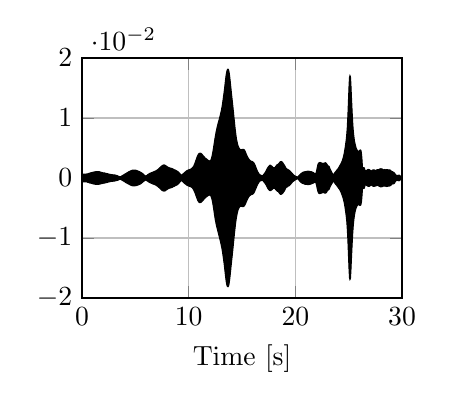
\begin{tikzpicture}

\begin{axis}[%
width=1.6in,
height=1.2in,
at={(0.758in,0.481in)},
scale only axis,
xmin=0,
xmax=30,
xmajorgrids,
ymin=-0.02,
ymax=0.02,
ymajorgrids,
xlabel={Time [s]},
axis background/.style={fill=white}
]
\addplot[fill=black,draw=black,forget plot] plot table[row sep=crcr]{%
2.08333333333333e-05	0.00127804279327393\\
0.0417454218822439	0.000631213188171387\\
0.0834700104311544	0.000625014305114746\\
0.125194598980065	0.000635147094726563\\
0.166919187528975	0.000628471374511719\\
0.208643776077886	0.000626802444458008\\
0.250368364626797	0.000621795654296875\\
0.292092953175707	0.000622868537902832\\
0.333817541724618	0.000628829002380371\\
0.375542130273528	0.000621318817138672\\
0.417266718822439	0.000651001930236816\\
0.458991307371349	0.000663518905639648\\
0.50071589592026	0.000679612159729004\\
0.54244048446917	0.000688552856445313\\
0.584165073018081	0.000703096389770508\\
0.625889661566991	0.000748038291931152\\
0.667614250115902	0.000764727592468262\\
0.709338838664812	0.000782251358032227\\
0.751063427213723	0.000815749168395996\\
0.792788015762633	0.000848770141601563\\
0.834512604311544	0.000861644744873047\\
0.876237192860454	0.000872373580932617\\
0.917961781409365	0.000892996788024902\\
0.959686369958275	0.000927567481994629\\
1.00141095850719	0.00093841552734375\\
1.0431355470561	0.000953912734985352\\
1.08486013560501	0.000977635383605957\\
1.12658472415392	0.000986456871032715\\
1.16830931270283	0.00102269649505615\\
1.21003390125174	0.00102055072784424\\
1.25175848980065	0.00102221965789795\\
1.29348307834956	0.00104677677154541\\
1.33520766689847	0.00104153156280518\\
1.37693225544738	0.00103974342346191\\
1.41865684399629	0.00103652477264404\\
1.4603814325452	0.00104057788848877\\
1.50210602109411	0.00103223323822021\\
1.54383060964302	0.00104439258575439\\
1.58555519819193	0.00103390216827393\\
1.62727978674084	0.00102889537811279\\
1.66900437528975	0.000995635986328125\\
1.71072896383866	0.000981450080871582\\
1.75245355238758	0.000968337059020996\\
1.79417814093649	0.000933051109313965\\
1.8359027294854	0.000915884971618652\\
1.87762731803431	0.000895857810974121\\
1.91935190658322	0.000874638557434082\\
1.96107649513213	0.000847458839416504\\
2.00280108368104	0.000832915306091309\\
2.04452567222995	0.000840663909912109\\
2.08625026077886	0.000831246376037598\\
2.12797484932777	0.000821232795715332\\
2.16969943787668	0.000807404518127441\\
2.21142402642559	0.000768899917602539\\
2.2531486149745	0.000757694244384766\\
2.29487320352341	0.000733017921447754\\
2.33659779207232	0.000726103782653809\\
2.37832238062123	0.000716090202331543\\
2.42004696917014	0.000691056251525879\\
2.46177155771905	0.000661253929138184\\
2.50349614626796	0.000634193420410156\\
2.54522073481687	0.00062716007232666\\
2.58694532336579	0.000597119331359863\\
2.6286699119147	0.000601649284362793\\
2.67039450046361	0.000583291053771973\\
2.71211908901252	0.000567436218261719\\
2.75384367756143	0.000557541847229004\\
2.79556826611034	0.000541567802429199\\
2.83729285465925	0.000536680221557617\\
2.87901744320816	0.000523209571838379\\
2.92074203175707	0.000514030456542969\\
2.96246662030598	0.000505685806274414\\
3.00419120885489	0.000509381294250488\\
3.0459157974038	0.000492453575134277\\
3.08764038595271	0.000486135482788086\\
3.12936497450162	0.000458955764770508\\
3.17108956305053	0.000441431999206543\\
3.21281415159944	0.000431060791015625\\
3.25453874014835	0.000412344932556152\\
3.29626332869726	0.000388026237487793\\
3.33798791724618	0.000339627265930176\\
3.37971250579509	0.000316739082336426\\
3.421437094344	0.000280022621154785\\
3.46316168289291	0.000258326530456543\\
3.50488627144182	0.000225305557250977\\
3.54661085999073	0.000218987464904785\\
3.58833544853964	0.000194072723388672\\
3.63006003708855	0.000222444534301758\\
3.67178462563746	0.000257372856140137\\
3.71350921418637	0.000302910804748535\\
3.75523380273528	0.000357985496520996\\
3.79695839128419	0.000406026840209961\\
3.8386829798331	0.00044560432434082\\
3.88040756838201	0.000483155250549316\\
3.92213215693092	0.000528216361999512\\
3.96385674547983	0.000562429428100586\\
4.00558133402874	0.00061953067779541\\
4.04730592257765	0.000665068626403809\\
4.08903051112656	0.000702261924743652\\
4.13075509967547	0.000744342803955078\\
4.17247968822439	0.000792741775512695\\
4.2142042767733	0.0008544921875\\
4.25592886532221	0.000883221626281738\\
4.29765345387112	0.000934243202209473\\
4.33937804242003	0.000978946685791016\\
4.38110263096894	0.00101733207702637\\
4.42282721951785	0.00105810165405273\\
4.46455180806676	0.00109744071960449\\
4.50627639661567	0.00111865997314453\\
4.54800098516458	0.00115501880645752\\
4.58972557371349	0.00120365619659424\\
4.6314501622624	0.00122451782226563\\
4.67317475081131	0.00125038623809814\\
4.71489933936022	0.00128710269927979\\
4.75662392790913	0.00128340721130371\\
4.79834851645804	0.00130021572113037\\
4.84007310500695	0.00130677223205566\\
4.88179769355586	0.00130546092987061\\
4.92352228210478	0.00130975246429443\\
4.96524687065368	0.00129389762878418\\
5.0069714592026	0.00129055976867676\\
5.04869604775151	0.00127255916595459\\
5.09042063630042	0.00126254558563232\\
5.13214522484933	0.00122177600860596\\
5.17386981339824	0.00119674205780029\\
5.21559440194715	0.00117611885070801\\
5.25731899049606	0.00114655494689941\\
5.29904357904497	0.00110149383544922\\
5.34076816759388	0.00109362602233887\\
5.38249275614279	0.00103819370269775\\
5.4242173446917	0.00101065635681152\\
5.46594193324061	0.000965595245361328\\
5.50766652178952	0.000915408134460449\\
5.54939111033843	0.000874519348144531\\
5.59111569888734	0.000841140747070313\\
5.63284028743625	0.000781059265136719\\
5.67456487598516	0.000725507736206055\\
5.71628946453407	0.000658035278320313\\
5.75801405308299	0.000604987144470215\\
5.7997386416319	0.000518560409545898\\
5.84146323018081	0.000460147857666016\\
5.88318781872972	0.000397682189941406\\
5.92491240727863	0.00036311149597168\\
5.96663699582754	0.000349760055541992\\
6.00836158437645	0.000349640846252441\\
6.05008617292536	0.000375509262084961\\
6.09181076147427	0.000434398651123047\\
6.13353535002318	0.000504136085510254\\
6.17525993857209	0.000555276870727539\\
6.216984527121	0.00062251091003418\\
6.25870911566991	0.000640511512756348\\
6.30043370421882	0.000700473785400391\\
6.34215829276773	0.000741958618164063\\
6.38388288131664	0.000778675079345703\\
6.42560746986555	0.000809073448181152\\
6.46733205841446	0.000843644142150879\\
6.50905664696338	0.000872969627380371\\
6.55078123551229	0.00089871883392334\\
6.5925058240612	0.000939726829528809\\
6.63423041261011	0.000955104827880859\\
6.67595500115902	0.00098717212677002\\
6.71767958970793	0.00101554393768311\\
6.75940417825684	0.00105273723602295\\
6.80112876680575	0.00108933448791504\\
6.84285335535466	0.00110065937042236\\
6.88457794390357	0.00114583969116211\\
6.92630253245248	0.00117993354797363\\
6.96802712100139	0.00121629238128662\\
7.0097517095503	0.00127542018890381\\
7.05147629809921	0.00132966041564941\\
7.09320088664812	0.00136947631835938\\
7.13492547519703	0.0014340877532959\\
7.17665006374594	0.00149333477020264\\
7.21837465229485	0.00157928466796875\\
7.26009924084376	0.00163924694061279\\
7.30182382939268	0.00172519683837891\\
7.34354841794159	0.00178694725036621\\
7.3852730064905	0.00186848640441895\\
7.42699759503941	0.00191104412078857\\
7.46872218358832	0.00197887420654297\\
7.51044677213723	0.00203204154968262\\
7.55217136068614	0.00209450721740723\\
7.59389594923505	0.00211906433105469\\
7.63562053778396	0.0021517276763916\\
7.67734512633287	0.00215578079223633\\
7.71906971488178	0.00215423107147217\\
7.76079430343069	0.00213372707366943\\
7.8025188919796	0.0020899772644043\\
7.84424348052851	0.00203394889831543\\
7.88596806907742	0.00199556350708008\\
7.92769265762633	0.00193679332733154\\
7.96941724617524	0.00188601016998291\\
8.01114183472416	0.00183010101318359\\
8.05286642327307	0.00178492069244385\\
8.09459101182198	0.00175571441650391\\
8.13631560037089	0.00172579288482666\\
8.1780401889198	0.00169909000396729\\
8.21976477746871	0.00166606903076172\\
8.26148936601762	0.00164306163787842\\
8.30321395456653	0.00163936614990234\\
8.34493854311544	0.00160729885101318\\
8.38666313166435	0.00157511234283447\\
8.42838772021326	0.00156009197235107\\
8.47011230876217	0.0015329122543335\\
8.51183689731108	0.00149202346801758\\
8.55356148585999	0.0014570951461792\\
8.5952860744089	0.00141036510467529\\
8.63701066295781	0.00136888027191162\\
8.67873525150672	0.00133645534515381\\
8.72045984005563	0.00132477283477783\\
8.76218442860454	0.00127542018890381\\
8.80390901715345	0.00122463703155518\\
8.84563360570237	0.00119531154632568\\
8.88735819425128	0.0011591911315918\\
8.92908278280018	0.00110948085784912\\
8.9708073713491	0.00105977058410645\\
9.01253195989801	0.00100851058959961\\
9.05425654844692	0.000942230224609375\\
9.09598113699583	0.000854015350341797\\
9.13770572554474	0.000771164894104004\\
9.17943031409365	0.000705480575561523\\
9.22115490264256	0.000602602958679199\\
9.26287949119147	0.000526070594787598\\
9.30460407974038	0.000465273857116699\\
9.34632866828929	0.000481009483337402\\
9.3880532568382	0.000534534454345703\\
9.42977784538711	0.000605940818786621\\
9.47150243393602	0.000667691230773926\\
9.51322702248493	0.000735163688659668\\
9.55495161103384	0.000798940658569336\\
9.59667619958275	0.000867486000061035\\
9.63840078813166	0.000937104225158691\\
9.68012537668058	0.000984668731689453\\
9.72184996522949	0.00106942653656006\\
9.7635745537784	0.00111746788024902\\
9.80529914232731	0.00117456912994385\\
9.84702373087622	0.00122499465942383\\
9.88874831942513	0.00126338005065918\\
9.93047290797404	0.00129258632659912\\
9.97219749652295	0.00134050846099854\\
10.0139220850719	0.00134932994842529\\
10.0556466736208	0.00137102603912354\\
10.0973712621697	0.0014040470123291\\
10.1390958507186	0.00142395496368408\\
10.1808204392675	0.00145864486694336\\
10.2225450278164	0.00151920318603516\\
10.2642696163653	0.00155460834503174\\
10.3059942049142	0.00160431861877441\\
10.3477187934631	0.0016859769821167\\
10.3894433820121	0.00176119804382324\\
10.431167970561	0.00186002254486084\\
10.4728925591099	0.00198805332183838\\
10.5146171476588	0.00213873386383057\\
10.5563417362077	0.00231361389160156\\
10.5980663247566	0.00249052047729492\\
10.6397909133055	0.00271880626678467\\
10.6815155018544	0.0029449462890625\\
10.7232400904033	0.003135085105896\\
10.7649646789523	0.00335073471069336\\
10.8066892675012	0.00357913970947266\\
10.8484138560501	0.00374186038970947\\
10.890138444599	0.00388526916503906\\
10.9318630331479	0.00398504734039307\\
10.9735876216968	0.00407087802886963\\
11.0153122102457	0.00409936904907227\\
11.0570367987946	0.00411760807037354\\
11.0987613873435	0.00410938262939453\\
11.1404859758924	0.00409233570098877\\
11.1822105644414	0.00403416156768799\\
11.2239351529903	0.00398910045623779\\
11.2656597415392	0.00389575958251953\\
11.3073843300881	0.00380027294158936\\
11.349108918637	0.00370848178863525\\
11.3908335071859	0.0036165714263916\\
11.4325580957348	0.00354766845703125\\
11.4742826842837	0.00347673892974854\\
11.5160072728326	0.00337421894073486\\
11.5577318613816	0.00328707695007324\\
11.5994564499305	0.00325310230255127\\
11.6411810384794	0.0031893253326416\\
11.6829056270283	0.00314855575561523\\
11.7246302155772	0.00309467315673828\\
11.7663548041261	0.00300943851470947\\
11.808079392675	0.00295102596282959\\
11.8498039812239	0.0028998851776123\\
11.8915285697728	0.00287175178527832\\
11.9332531583217	0.00284099578857422\\
11.9749777468707	0.00283515453338623\\
12.0167023354196	0.0028756856918335\\
12.0584269239685	0.0029294490814209\\
12.1001515125174	0.00305366516113281\\
12.1418761010663	0.00328326225280762\\
12.1836006896152	0.003562331199646\\
12.2253252781641	0.00393486022949219\\
12.267049866713	0.00432932376861572\\
12.3087744552619	0.00478744506835938\\
12.3504990438108	0.00525879859924316\\
12.3922236323598	0.0057370662689209\\
12.4339482209087	0.00622677803039551\\
12.4756728094576	0.00669920444488525\\
12.5173973980065	0.00710928440093994\\
12.5591219865554	0.0075230598449707\\
12.6008465751043	0.00789737701416016\\
12.6425711636532	0.00824654102325439\\
12.6842957522021	0.00855863094329834\\
12.726020340751	0.00884735584259033\\
12.7677449293	0.00915205478668213\\
12.8094695178489	0.00941121578216553\\
12.8511941063978	0.00967514514923096\\
12.8929186949467	0.00999438762664795\\
12.9346432834956	0.0102517604827881\\
12.9763678720445	0.0105814933776855\\
13.0180924605934	0.0108782052993774\\
13.0598170491423	0.011201024055481\\
13.1015416376912	0.0115941762924194\\
13.1432662262401	0.012012243270874\\
13.1849908147891	0.0125203132629395\\
13.226715403338	0.0130273103713989\\
13.2684399918869	0.0136046409606934\\
13.3101645804358	0.0141032934188843\\
13.3518891689847	0.0147042274475098\\
13.3936137575336	0.0153554677963257\\
13.4353383460825	0.0160462856292725\\
13.4770629346314	0.0166767835617065\\
13.5187875231803	0.0172096490859985\\
13.5605121117293	0.0176523923873901\\
13.6022367002782	0.0179364681243896\\
13.6439612888271	0.0181000232696533\\
13.685685877376	0.0181249380111694\\
13.7274104659249	0.0180306434631348\\
13.7691350544738	0.0177460908889771\\
13.8108596430227	0.0172954797744751\\
13.8525842315716	0.0166802406311035\\
13.8943088201205	0.0160108804702759\\
13.9360334086694	0.0152887105941772\\
13.9777579972184	0.014556884765625\\
14.0194825857673	0.0138355493545532\\
14.0612071743162	0.0131707191467285\\
14.1029317628651	0.012508749961853\\
14.144656351414	0.0117968320846558\\
14.1863809399629	0.0111017227172852\\
14.2281055285118	0.0103411674499512\\
14.2698301170607	0.00961518287658691\\
14.3115547056096	0.00887918472290039\\
14.3532792941586	0.0081636905670166\\
14.3950038827075	0.00755643844604492\\
14.4367284712564	0.00697898864746094\\
14.4784530598053	0.00649642944335938\\
14.5201776483542	0.0061107873916626\\
14.5619022369031	0.00577616691589355\\
14.603626825452	0.00548958778381348\\
14.6453514140009	0.00526928901672363\\
14.6870760025498	0.00509107112884521\\
14.7288005910988	0.00496208667755127\\
14.7705251796477	0.00485360622406006\\
14.8122497681966	0.00475609302520752\\
14.8539743567455	0.00471067428588867\\
14.8956989452944	0.00469815731048584\\
14.9374235338433	0.00469648838043213\\
14.9791481223922	0.00470972061157227\\
15.0208727109411	0.00475072860717773\\
15.06259729949	0.00476610660552979\\
15.1043218880389	0.00477027893066406\\
15.1460464765879	0.00474727153778076\\
15.1877710651368	0.00470900535583496\\
15.2294956536857	0.0046459436416626\\
15.2712202422346	0.00450277328491211\\
15.3129448307835	0.00431835651397705\\
15.3546694193324	0.00414323806762695\\
15.3963940078813	0.00397789478302002\\
15.4381185964302	0.00377774238586426\\
15.4798431849791	0.00362992286682129\\
15.521567773528	0.00346171855926514\\
15.563292362077	0.00334203243255615\\
15.6050169506259	0.00322949886322021\\
15.6467415391748	0.00311958789825439\\
15.6884661277237	0.0030292272567749\\
15.7301907162726	0.00293910503387451\\
15.7719153048215	0.00287222862243652\\
15.8136398933704	0.00282394886016846\\
15.8553644819193	0.00278961658477783\\
15.8970890704682	0.00276505947113037\\
15.9388136590172	0.00274670124053955\\
15.9805382475661	0.00270199775695801\\
16.022262836115	0.00265073776245117\\
16.0639874246639	0.00259053707122803\\
16.1057120132128	0.00251424312591553\\
16.1474366017617	0.00238251686096191\\
16.1891611903106	0.00223147869110107\\
16.2308857788595	0.00208532810211182\\
16.2726103674084	0.0018693208694458\\
16.3143349559573	0.00169098377227783\\
16.3560595445063	0.00147318840026855\\
16.3977841330552	0.00132143497467041\\
16.4395087216041	0.00113749504089355\\
16.481233310153	0.00098264217376709\\
16.5229578987019	0.000874996185302734\\
16.5646824872508	0.000738620758056641\\
16.6064070757997	0.000650525093078613\\
16.6481316643486	0.00056755542755127\\
16.6898562528975	0.000516533851623535\\
16.7315808414465	0.000478267669677734\\
16.7733054299954	0.000433444976806641\\
16.8150300185443	0.000414729118347168\\
16.8567546070932	0.000384330749511719\\
16.8984791956421	0.00037682056427002\\
16.940203784191	0.000384211540222168\\
16.9819283727399	0.000468611717224121\\
17.0236529612888	0.00055539608001709\\
17.0653775498377	0.000656843185424805\\
17.1071021383867	0.000748038291931152\\
17.1488267269356	0.000851631164550781\\
17.1905513154845	0.000960946083068848\\
17.2322759040334	0.0010915994644165\\
17.2740004925823	0.00124549865722656\\
17.3157250811312	0.00138700008392334\\
17.3574496696801	0.0015188455581665\\
17.399174258229	0.00166404247283936\\
17.4408988467779	0.00178706645965576\\
17.4826234353268	0.0018768310546875\\
17.5243480238758	0.00198018550872803\\
17.5660726124247	0.00205063819885254\\
17.6077972009736	0.00211203098297119\\
17.6495217895225	0.00213837623596191\\
17.6912463780714	0.00209248065948486\\
17.7329709666203	0.00203239917755127\\
17.7746955551692	0.00196850299835205\\
17.8164201437181	0.00189638137817383\\
17.858144732267	0.00183045864105225\\
17.8998693208159	0.0017702579498291\\
17.9415939093649	0.00172531604766846\\
17.9833184979138	0.00170111656188965\\
18.0250430864627	0.0017085075378418\\
18.0667676750116	0.00173532962799072\\
18.1084922635605	0.00178778171539307\\
18.1502168521094	0.00189721584320068\\
18.1919414406583	0.00199604034423828\\
18.2336660292072	0.00208830833435059\\
18.2753906177561	0.00217342376708984\\
18.3171152063051	0.00222349166870117\\
18.358839794854	0.00226426124572754\\
18.4005643834029	0.00230693817138672\\
18.4422889719518	0.00237786769866943\\
18.4840135605007	0.00247800350189209\\
18.5257381490496	0.00257432460784912\\
18.5674627375985	0.0026702880859375\\
18.6091873261474	0.00271201133728027\\
18.6509119146963	0.00272214412689209\\
18.6926365032453	0.0027320384979248\\
18.7343610917942	0.00268161296844482\\
18.7760856803431	0.00261020660400391\\
18.817810268892	0.00252974033355713\\
18.8595348574409	0.00240576267242432\\
18.9012594459898	0.00229310989379883\\
18.9429840345387	0.00217711925506592\\
18.9847086230876	0.0020749568939209\\
19.0264332116365	0.00192344188690186\\
19.0681578001854	0.00179409980773926\\
19.1098823887344	0.00164484977722168\\
19.1516069772833	0.0015639066696167\\
19.1933315658322	0.00151050090789795\\
19.2350561543811	0.00147199630737305\\
19.27678074293	0.00143206119537354\\
19.3185053314789	0.00135934352874756\\
19.3602299200278	0.00132179260253906\\
19.4019545085767	0.00131142139434814\\
19.4436790971256	0.00124466419219971\\
19.4854036856745	0.00116324424743652\\
19.5271282742235	0.00109946727752686\\
19.5688528627724	0.00101351737976074\\
19.6105774513213	0.000917196273803711\\
19.6523020398702	0.000830292701721191\\
19.6940266284191	0.000766158103942871\\
19.735751216968	0.00069272518157959\\
19.7774758055169	0.000599980354309082\\
19.8192003940658	0.000518560409545898\\
19.8609249826147	0.000458955764770508\\
19.9026495711637	0.000408053398132324\\
19.9443741597126	0.000364780426025391\\
19.9860987482615	0.000320792198181152\\
20.0278233368104	0.000272393226623535\\
20.0695479253593	0.000250339508056641\\
20.1112725139082	0.000214934349060059\\
20.1529971024571	0.000171542167663574\\
20.194721691006	0.000146985054016113\\
20.2364462795549	0.000164389610290527\\
20.2781708681038	0.000265717506408691\\
20.3198954566528	0.000333309173583984\\
20.3616200452017	0.000410079956054688\\
20.4033446337506	0.000494480133056641\\
20.4450692222995	0.000574469566345215\\
20.4867938108484	0.000638842582702637\\
20.5285183993973	0.000702261924743652\\
20.5702429879462	0.000772714614868164\\
20.6119675764951	0.000812888145446777\\
20.653692165044	0.000873804092407227\\
20.695416753593	0.000924110412597656\\
20.7371413421419	0.000951766967773438\\
20.7788659306908	0.000968456268310547\\
20.8205905192397	0.00100481510162354\\
20.8623151077886	0.00101923942565918\\
20.9040396963375	0.00103354454040527\\
20.9457642848864	0.00104677677154541\\
20.9874888734353	0.00106978416442871\\
21.0292134619842	0.00108063220977783\\
21.0709380505331	0.00110197067260742\\
21.1126626390821	0.00110578536987305\\
21.154387227631	0.00111269950866699\\
21.1961118161799	0.0011211633682251\\
21.2378364047288	0.00109267234802246\\
21.2795609932777	0.00110900402069092\\
21.3212855818266	0.0010993480682373\\
21.3630101703755	0.00107061862945557\\
21.4047347589244	0.00106143951416016\\
21.4464593474733	0.00103640556335449\\
21.4881839360223	0.00104343891143799\\
21.5299085245712	0.00100553035736084\\
21.5716331131201	0.000985622406005859\\
21.613357701669	0.000940918922424316\\
21.6550822902179	0.000916361808776855\\
21.6968068787668	0.000889897346496582\\
21.7385314673157	0.000823616981506348\\
21.7802560558646	0.000762343406677246\\
21.8219806444135	0.000701904296875\\
21.8637052329624	0.000655055046081543\\
21.9054298215114	0.000687241554260254\\
21.9471544100603	0.000838160514831543\\
21.9888789986092	0.00113999843597412\\
22.0306035871581	0.00152075290679932\\
22.072328175707	0.00187468528747559\\
22.1140527642559	0.00221681594848633\\
22.1557773528048	0.00239455699920654\\
22.1975019413537	0.00249767303466797\\
22.2392265299026	0.00254964828491211\\
22.2809511184516	0.00256383419036865\\
22.3226757070005	0.00257682800292969\\
22.3644002955494	0.00254476070404053\\
22.4061248840983	0.00252056121826172\\
22.4478494726472	0.00248932838439941\\
22.4895740611961	0.00247585773468018\\
22.531298649745	0.00244200229644775\\
22.5730232382939	0.00242948532104492\\
22.6147478268428	0.00242924690246582\\
22.6564724153917	0.00244510173797607\\
22.6981970039407	0.00247335433959961\\
22.7399215924896	0.00249636173248291\\
22.7816461810385	0.00252437591552734\\
22.8233707695874	0.00253105163574219\\
22.8650953581363	0.00247752666473389\\
22.9068199466852	0.00240111351013184\\
22.9485445352341	0.00229179859161377\\
22.990269123783	0.00217175483703613\\
23.0319937123319	0.00206196308135986\\
23.0737183008809	0.00201737880706787\\
23.1154428894298	0.00197815895080566\\
23.1571674779787	0.001914381980896\\
23.1988920665276	0.00174415111541748\\
23.2406166550765	0.00155723094940186\\
23.2823412436254	0.00137650966644287\\
23.3240658321743	0.00122785568237305\\
23.3657904207232	0.0011066198348999\\
23.4075150092721	0.000943422317504883\\
23.449239597821	0.000793099403381348\\
23.49096418637	0.000658512115478516\\
23.5326887749189	0.000577569007873535\\
23.5744133634678	0.000577449798583984\\
23.6161379520167	0.000663876533508301\\
23.6578625405656	0.000740528106689453\\
23.6995871291145	0.000880002975463867\\
23.7413117176634	0.00096583366394043\\
23.7830363062123	0.00106024742126465\\
23.8247608947612	0.00114238262176514\\
23.8664854833102	0.00124049186706543\\
23.9082100718591	0.00134313106536865\\
23.949934660408	0.00144410133361816\\
23.9916592489569	0.00151205062866211\\
24.0333838375058	0.00162482261657715\\
24.0751084260547	0.00174117088317871\\
24.1168330146036	0.00186669826507568\\
24.1585576031525	0.00199449062347412\\
24.2002821917014	0.00214552879333496\\
24.2420067802503	0.00225734710693359\\
24.2837313687993	0.00240910053253174\\
24.3254559573482	0.00255143642425537\\
24.3671805458971	0.00274038314819336\\
24.408905134446	0.0029289722442627\\
24.4506297229949	0.00315427780151367\\
24.4923543115438	0.00340795516967773\\
24.5340789000927	0.00371301174163818\\
24.5758034886416	0.00405347347259521\\
24.6175280771905	0.004477858543396\\
24.6592526657395	0.00492167472839355\\
24.7009772542884	0.00541150569915771\\
24.7427018428373	0.0059894323348999\\
24.7844264313862	0.00655853748321533\\
24.8261510199351	0.007362961769104\\
24.867875608484	0.00837421417236328\\
24.9096001970329	0.00980007648468018\\
24.9513247855818	0.0114856958389282\\
24.9930493741307	0.0134135484695435\\
25.0347739626796	0.0153409242630005\\
25.0764985512286	0.0167388916015625\\
25.1182231397775	0.0170340538024902\\
25.1599477283264	0.0168673992156982\\
25.2016723168753	0.0156699419021606\\
25.2433969054242	0.0138726234436035\\
25.2851214939731	0.0123008489608765\\
25.326846082522	0.0107371807098389\\
25.3685706710709	0.00932610034942627\\
25.4102952596198	0.00820529460906982\\
25.4520198481687	0.00739765167236328\\
25.4937444367177	0.00674927234649658\\
25.5354690252666	0.00620806217193604\\
25.5771936138155	0.0058283805847168\\
25.6189182023644	0.00549626350402832\\
25.6606427909133	0.00521326065063477\\
25.7023673794622	0.00496041774749756\\
25.7440919680111	0.00478363037109375\\
25.78581655656	0.00464761257171631\\
25.8275411451089	0.0045546293258667\\
25.8692657336579	0.00447988510131836\\
25.9109903222068	0.00443220138549805\\
25.9527149107557	0.00445985794067383\\
25.9944394993046	0.00450396537780762\\
26.0361640878535	0.00461125373840332\\
26.0778886764024	0.00466263294219971\\
26.1196132649513	0.00464582443237305\\
26.1613378535002	0.00447726249694824\\
26.2030624420491	0.0039064884185791\\
26.2447870305981	0.00300025939941406\\
26.286511619147	0.00182676315307617\\
26.3282362076959	0.00153994560241699\\
26.3699607962448	0.00165724754333496\\
26.4116853847937	0.00171065330505371\\
26.4534099733426	0.00168359279632568\\
26.4951345618915	0.00149905681610107\\
26.5368591504404	0.00116610527038574\\
26.5785837389893	0.00111997127532959\\
26.6203083275383	0.00118911266326904\\
26.6620329160872	0.0012211799621582\\
26.7037575046361	0.00127851963043213\\
26.745482093185	0.00134193897247314\\
26.7872066817339	0.00138437747955322\\
26.8289312702828	0.00141060352325439\\
26.8706558588317	0.00138974189758301\\
26.9123804473806	0.00137734413146973\\
26.9541050359295	0.00135815143585205\\
26.9958296244784	0.00130808353424072\\
27.0375542130274	0.00120711326599121\\
27.0792788015763	0.00111997127532959\\
27.1210033901252	0.00116991996765137\\
27.1627279786741	0.00122678279876709\\
27.204452567223	0.00126850605010986\\
27.2461771557719	0.0013127326965332\\
27.2879017443208	0.00134360790252686\\
27.3296263328697	0.00133943557739258\\
27.3713509214186	0.00133466720581055\\
27.4130755099675	0.00132310390472412\\
27.4548000985165	0.0012892484664917\\
27.4965246870654	0.00125885009765625\\
27.5382492756143	0.00125181674957275\\
27.5799738641632	0.00126266479492188\\
27.6216984527121	0.00133514404296875\\
27.663423041261	0.00136935710906982\\
27.7051476298099	0.00139367580413818\\
27.7468722183588	0.00139355659484863\\
27.7885968069077	0.00139641761779785\\
27.8303213954567	0.00139939785003662\\
27.8720459840056	0.0014498233795166\\
27.9137705725545	0.0014873743057251\\
27.9554951611034	0.00151157379150391\\
27.9972197496523	0.00152623653411865\\
28.0389443382012	0.00152468681335449\\
28.0806689267501	0.00151371955871582\\
28.122393515299	0.00149452686309814\\
28.1641181038479	0.00145208835601807\\
28.2058426923968	0.00135600566864014\\
28.2475672809458	0.00132095813751221\\
28.2892918694947	0.00136649608612061\\
28.3310164580436	0.00140035152435303\\
28.3727410465925	0.0013735294342041\\
28.4144656351414	0.00135397911071777\\
28.4561902236903	0.0013434886932373\\
28.4979148122392	0.00136935710906982\\
28.5396394007881	0.00138866901397705\\
28.581363989337	0.00139319896697998\\
28.623088577886	0.00137901306152344\\
28.6648131664349	0.00135350227355957\\
28.7065377549838	0.00134694576263428\\
28.7482623435327	0.0013422966003418\\
28.7899869320816	0.00135385990142822\\
28.8317115206305	0.00134527683258057\\
28.8734361091794	0.00130677223205566\\
28.9151606977283	0.0012671947479248\\
28.9568852862772	0.00120365619659424\\
28.9986098748261	0.00113034248352051\\
29.0403344633751	0.00106322765350342\\
29.082059051924	0.00106358528137207\\
29.1237836404729	0.00101351737976074\\
29.1655082290218	0.000969767570495605\\
29.2072328175707	0.000931739807128906\\
29.2489574061196	0.000900745391845703\\
29.2906819946685	0.000811934471130371\\
29.3324065832174	0.000694751739501953\\
29.3741311717663	0.000607967376708984\\
29.4158557603153	0.000501155853271484\\
29.4575803488642	0.000453591346740723\\
29.4993049374131	0.000370621681213379\\
29.541029525962	0.000379204750061035\\
29.5827541145109	0.000430107116699219\\
29.6244787030598	0.00041806697845459\\
29.6662032916087	0.000442385673522949\\
29.7079278801576	0.000470161437988281\\
29.7496524687065	0.000450968742370605\\
29.7913770572554	0.000368475914001465\\
29.8331016458044	0.000347614288330078\\
29.8748262343533	0.000216484069824219\\
29.9165508229022	0.000200271606445313\\
29.9582754114511	0.000146865844726563\\
30	0.000100493431091309\\
}
\closedcycle;
\addplot[fill=black,draw=black,forget plot] plot table[row sep=crcr]{%
2.08333333333333e-05	-0.00102686882019043\\
0.0417454218822439	-0.000666379928588867\\
0.0834700104311544	-0.000653386116027832\\
0.125194598980065	-0.000644683837890625\\
0.166919187528975	-0.000635027885437012\\
0.208643776077886	-0.000647187232971191\\
0.250368364626797	-0.000632405281066895\\
0.292092953175707	-0.00063621997833252\\
0.333817541724618	-0.000647187232971191\\
0.375542130273528	-0.000648021697998047\\
0.417266718822439	-0.000648260116577148\\
0.458991307371349	-0.000664114952087402\\
0.50071589592026	-0.00068211555480957\\
0.54244048446917	-0.000726819038391113\\
0.584165073018081	-0.000746726989746094\\
0.625889661566991	-0.00075685977935791\\
0.667614250115902	-0.000790715217590332\\
0.709338838664812	-0.00079190731048584\\
0.751063427213723	-0.000853300094604492\\
0.792788015762633	-0.000846028327941895\\
0.834512604311544	-0.000860214233398438\\
0.876237192860454	-0.000890254974365234\\
0.917961781409365	-0.000910758972167969\\
0.959686369958275	-0.000927567481994629\\
1.00141095850719	-0.000959515571594238\\
1.0431355470561	-0.000976800918579102\\
1.08486013560501	-0.000985383987426758\\
1.12658472415392	-0.00101625919342041\\
1.16830931270283	-0.00102126598358154\\
1.21003390125174	-0.00101637840270996\\
1.25175848980065	-0.00104856491088867\\
1.29348307834956	-0.00104689598083496\\
1.33520766689847	-0.00107026100158691\\
1.37693225544738	-0.00106298923492432\\
1.41865684399629	-0.00106143951416016\\
1.4603814325452	-0.0010751485824585\\
1.50210602109411	-0.00105762481689453\\
1.54383060964302	-0.00104224681854248\\
1.58555519819193	-0.00104773044586182\\
1.62727978674084	-0.00101590156555176\\
1.66900437528975	-0.00101542472839355\\
1.71072896383866	-0.000998497009277344\\
1.75245355238758	-0.000977516174316406\\
1.79417814093649	-0.000947475433349609\\
1.8359027294854	-0.000937104225158691\\
1.87762731803431	-0.000921726226806641\\
1.91935190658322	-0.000900387763977051\\
1.96107649513213	-0.000885844230651855\\
2.00280108368104	-0.000869870185852051\\
2.04452567222995	-0.000851869583129883\\
2.08625026077886	-0.000850319862365723\\
2.12797484932777	-0.000836014747619629\\
2.16969943787668	-0.000826478004455566\\
2.21142402642559	-0.000801920890808105\\
2.2531486149745	-0.000780701637268066\\
2.29487320352341	-0.000770926475524902\\
2.33659779207232	-0.00075066089630127\\
2.37832238062123	-0.000723123550415039\\
2.42004696917014	-0.000699996948242188\\
2.46177155771905	-0.000677227973937988\\
2.50349614626796	-0.000650525093078613\\
2.54522073481687	-0.000636696815490723\\
2.58694532336579	-0.000627517700195313\\
2.6286699119147	-0.000609159469604492\\
2.67039450046361	-0.000603795051574707\\
2.71211908901252	-0.000569581985473633\\
2.75384367756143	-0.000574469566345215\\
2.79556826611034	-0.000577807426452637\\
2.83729285465925	-0.000553607940673828\\
2.87901744320816	-0.000548124313354492\\
2.92074203175707	-0.00053560733795166\\
2.96246662030598	-0.000534415245056152\\
3.00419120885489	-0.000509023666381836\\
3.0459157974038	-0.000513076782226563\\
3.08764038595271	-0.000487208366394043\\
3.12936497450162	-0.000481367111206055\\
3.17108956305053	-0.000455498695373535\\
3.21281415159944	-0.000430583953857422\\
3.25453874014835	-0.00042271614074707\\
3.29626332869726	-0.000396370887756348\\
3.33798791724618	-0.000377535820007324\\
3.37971250579509	-0.0003662109375\\
3.421437094344	-0.000309467315673828\\
3.46316168289291	-0.000249028205871582\\
3.50488627144182	-0.000252366065979004\\
3.54661085999073	-0.000213146209716797\\
3.58833544853964	-0.000223159790039063\\
3.63006003708855	-0.000251650810241699\\
3.67178462563746	-0.000289201736450195\\
3.71350921418637	-0.000321149826049805\\
3.75523380273528	-0.000371217727661133\\
3.79695839128419	-0.000423431396484375\\
3.8386829798331	-0.000450491905212402\\
3.88040756838201	-0.000500679016113281\\
3.92213215693092	-0.000526070594787598\\
3.96385674547983	-0.000599026679992676\\
4.00558133402874	-0.000629186630249023\\
4.04730592257765	-0.000687122344970703\\
4.08903051112656	-0.000753521919250488\\
4.13075509967547	-0.000774025917053223\\
4.17247968822439	-0.000826478004455566\\
4.2142042767733	-0.000853180885314941\\
4.25592886532221	-0.00090491771697998\\
4.29765345387112	-0.000939130783081055\\
4.33937804242003	-0.000977635383605957\\
4.38110263096894	-0.00102019309997559\\
4.42282721951785	-0.00105965137481689\\
4.46455180806676	-0.00110352039337158\\
4.50627639661567	-0.00114989280700684\\
4.54800098516458	-0.00119566917419434\\
4.58972557371349	-0.0012061595916748\\
4.6314501622624	-0.00124907493591309\\
4.67317475081131	-0.00127971172332764\\
4.71489933936022	-0.00128829479217529\\
4.75662392790913	-0.00130546092987061\\
4.79834851645804	-0.00131499767303467\\
4.84007310500695	-0.00132215023040771\\
4.88179769355586	-0.00130057334899902\\
4.92352228210478	-0.00131082534790039\\
4.96524687065368	-0.00129926204681396\\
5.0069714592026	-0.00129044055938721\\
5.04869604775151	-0.00127971172332764\\
5.09042063630042	-0.00125789642333984\\
5.13214522484933	-0.00124466419219971\\
5.17386981339824	-0.00120401382446289\\
5.21559440194715	-0.00118374824523926\\
5.25731899049606	-0.0011669397354126\\
5.29904357904497	-0.0011293888092041\\
5.34076816759388	-0.00109195709228516\\
5.38249275614279	-0.00105810165405273\\
5.4242173446917	-0.00101017951965332\\
5.46594193324061	-0.00100290775299072\\
5.50766652178952	-0.000959157943725586\\
5.54939111033843	-0.000900030136108398\\
5.59111569888734	-0.00082850456237793\\
5.63284028743625	-0.000783085823059082\\
5.67456487598516	-0.000710010528564453\\
5.71628946453407	-0.000656366348266602\\
5.75801405308299	-0.000581622123718262\\
5.7997386416319	-0.000542402267456055\\
5.84146323018081	-0.000481128692626953\\
5.88318781872972	-0.000410914421081543\\
5.92491240727863	-0.000372648239135742\\
5.96663699582754	-0.000348806381225586\\
6.00836158437645	-0.000376343727111816\\
6.05008617292536	-0.000430464744567871\\
6.09181076147427	-0.000473618507385254\\
6.13353535002318	-0.000502347946166992\\
6.17525993857209	-0.000564455986022949\\
6.216984527121	-0.000625014305114746\\
6.25870911566991	-0.000676631927490234\\
6.30043370421882	-0.000699639320373535\\
6.34215829276773	-0.000757694244384766\\
6.38388288131664	-0.000777363777160645\\
6.42560746986555	-0.000813961029052734\\
6.46733205841446	-0.000852704048156738\\
6.50905664696338	-0.000889062881469727\\
6.55078123551229	-0.000915408134460449\\
6.5925058240612	-0.000960111618041992\\
6.63423041261011	-0.000981688499450684\\
6.67595500115902	-0.00102221965789795\\
6.71767958970793	-0.00103962421417236\\
6.75940417825684	-0.00105226039886475\\
6.80112876680575	-0.00108051300048828\\
6.84285335535466	-0.0011293888092041\\
6.88457794390357	-0.00115787982940674\\
6.92630253245248	-0.00120365619659424\\
6.96802712100139	-0.00123465061187744\\
7.0097517095503	-0.00132298469543457\\
7.05147629809921	-0.00133895874023438\\
7.09320088664812	-0.00139808654785156\\
7.13492547519703	-0.00146734714508057\\
7.17665006374594	-0.00152826309204102\\
7.21837465229485	-0.00159013271331787\\
7.26009924084376	-0.00165772438049316\\
7.30182382939268	-0.00171029567718506\\
7.34354841794159	-0.00177621841430664\\
7.3852730064905	-0.00184571743011475\\
7.42699759503941	-0.00194466114044189\\
7.46872218358832	-0.00201141834259033\\
7.51044677213723	-0.00208449363708496\\
7.55217136068614	-0.00210273265838623\\
7.59389594923505	-0.00214827060699463\\
7.63562053778396	-0.00216960906982422\\
7.67734512633287	-0.00217247009277344\\
7.71906971488178	-0.00217461585998535\\
7.76079430343069	-0.00214338302612305\\
7.8025188919796	-0.00213456153869629\\
7.84424348052851	-0.00208151340484619\\
7.88596806907742	-0.0020064115524292\\
7.92769265762633	-0.00198805332183838\\
7.96941724617524	-0.00190746784210205\\
8.01114183472416	-0.001861572265625\\
8.05286642327307	-0.00181961059570313\\
8.09459101182198	-0.0017857551574707\\
8.13631560037089	-0.00172650814056396\\
8.1780401889198	-0.00170445442199707\\
8.21976477746871	-0.00169551372528076\\
8.26148936601762	-0.0016704797744751\\
8.30321395456653	-0.00164508819580078\\
8.34493854311544	-0.00162088871002197\\
8.38666313166435	-0.00159966945648193\\
8.42838772021326	-0.0015636682510376\\
8.47011230876217	-0.00154459476470947\\
8.51183689731108	-0.00148701667785645\\
8.55356148585999	-0.00144493579864502\\
8.5952860744089	-0.00142264366149902\\
8.63701066295781	-0.0013965368270874\\
8.67873525150672	-0.00135350227355957\\
8.72045984005563	-0.00130546092987061\\
8.76218442860454	-0.00127053260803223\\
8.80390901715345	-0.00122749805450439\\
8.84563360570237	-0.00120830535888672\\
8.88735819425128	-0.00117897987365723\\
8.92908278280018	-0.00112974643707275\\
8.9708073713491	-0.00106942653656006\\
9.01253195989801	-0.00101053714752197\\
9.05425654844692	-0.000937938690185547\\
9.09598113699583	-0.000859379768371582\\
9.13770572554474	-0.000759363174438477\\
9.17943031409365	-0.000664949417114258\\
9.22115490264256	-0.000597000122070313\\
9.26287949119147	-0.000516057014465332\\
9.30460407974038	-0.000488877296447754\\
9.34632866828929	-0.000477790832519531\\
9.3880532568382	-0.00052487850189209\\
9.42977784538711	-0.000580787658691406\\
9.47150243393602	-0.000658869743347168\\
9.51322702248493	-0.000737667083740234\\
9.55495161103384	-0.000813484191894531\\
9.59667619958275	-0.000867843627929688\\
9.63840078813166	-0.000938653945922852\\
9.68012537668058	-0.00100386142730713\\
9.72184996522949	-0.00104475021362305\\
9.7635745537784	-0.00110816955566406\\
9.80529914232731	-0.00116312503814697\\
9.84702373087622	-0.00120985507965088\\
9.88874831942513	-0.00123989582061768\\
9.93047290797404	-0.00128579139709473\\
9.97219749652295	-0.00131833553314209\\
10.0139220850719	-0.00136172771453857\\
10.0556466736208	-0.001381516456604\\
10.0973712621697	-0.00140893459320068\\
10.1390958507186	-0.00143063068389893\\
10.1808204392675	-0.00146198272705078\\
10.2225450278164	-0.00147771835327148\\
10.2642696163653	-0.00153529644012451\\
10.3059942049142	-0.00158870220184326\\
10.3477187934631	-0.00164937973022461\\
10.3894433820121	-0.00176060199737549\\
10.431167970561	-0.00187122821807861\\
10.4728925591099	-0.00200474262237549\\
10.5146171476588	-0.0021744966506958\\
10.5563417362077	-0.00232183933258057\\
10.5980663247566	-0.00251173973083496\\
10.6397909133055	-0.00269830226898193\\
10.6815155018544	-0.0029139518737793\\
10.7232400904033	-0.00313377380371094\\
10.7649646789523	-0.00334537029266357\\
10.8066892675012	-0.00353193283081055\\
10.8484138560501	-0.00371968746185303\\
10.890138444599	-0.00384938716888428\\
10.9318630331479	-0.00397193431854248\\
10.9735876216968	-0.00406181812286377\\
11.0153122102457	-0.00410020351409912\\
11.0570367987946	-0.00410759449005127\\
11.0987613873435	-0.00409090518951416\\
11.1404859758924	-0.00406622886657715\\
11.1822105644414	-0.00400960445404053\\
11.2239351529903	-0.00394916534423828\\
11.2656597415392	-0.00386857986450195\\
11.3073843300881	-0.00379002094268799\\
11.349108918637	-0.00370407104492188\\
11.3908335071859	-0.0036236047744751\\
11.4325580957348	-0.00354516506195068\\
11.4742826842837	-0.00344586372375488\\
11.5160072728326	-0.00338876247406006\\
11.5577318613816	-0.00332152843475342\\
11.5994564499305	-0.00323891639709473\\
11.6411810384794	-0.00317728519439697\\
11.6829056270283	-0.00312745571136475\\
11.7246302155772	-0.00306165218353271\\
11.7663548041261	-0.00301694869995117\\
11.808079392675	-0.00295853614807129\\
11.8498039812239	-0.00291883945465088\\
11.8915285697728	-0.00288307666778564\\
11.9332531583217	-0.00284183025360107\\
11.9749777468707	-0.00283873081207275\\
12.0167023354196	-0.0028759241104126\\
12.0584269239685	-0.00294196605682373\\
12.1001515125174	-0.00307118892669678\\
12.1418761010663	-0.00330114364624023\\
12.1836006896152	-0.00355470180511475\\
12.2253252781641	-0.0038834810256958\\
12.267049866713	-0.00428617000579834\\
12.3087744552619	-0.00474965572357178\\
12.3504990438108	-0.00524497032165527\\
12.3922236323598	-0.00576281547546387\\
12.4339482209087	-0.00625550746917725\\
12.4756728094576	-0.00673317909240723\\
12.5173973980065	-0.00715768337249756\\
12.5591219865554	-0.00754010677337646\\
12.6008465751043	-0.00790107250213623\\
12.6425711636532	-0.00821995735168457\\
12.6842957522021	-0.00850951671600342\\
12.726020340751	-0.0088123083114624\\
12.7677449293	-0.00910806655883789\\
12.8094695178489	-0.00936484336853027\\
12.8511941063978	-0.00968718528747559\\
12.8929186949467	-0.00997006893157959\\
12.9346432834956	-0.0102742910385132\\
12.9763678720445	-0.0105773210525513\\
13.0180924605934	-0.0108996629714966\\
13.0598170491423	-0.0112502574920654\\
13.1015416376912	-0.01160728931427\\
13.1432662262401	-0.0120183229446411\\
13.1849908147891	-0.0124727487564087\\
13.226715403338	-0.0130163431167603\\
13.2684399918869	-0.0135517120361328\\
13.3101645804358	-0.0140920877456665\\
13.3518891689847	-0.0147049427032471\\
13.3936137575336	-0.015393853187561\\
13.4353383460825	-0.0160497426986694\\
13.4770629346314	-0.0166763067245483\\
13.5187875231803	-0.0172429084777832\\
13.5605121117293	-0.0176646709442139\\
13.6022367002782	-0.0179964303970337\\
13.6439612888271	-0.0181025266647339\\
13.685685877376	-0.0181208848953247\\
13.7274104659249	-0.0180073976516724\\
13.7691350544738	-0.0177512168884277\\
13.8108596430227	-0.0172833204269409\\
13.8525842315716	-0.0167142152786255\\
13.8943088201205	-0.0160259008407593\\
13.9360334086694	-0.0153111219406128\\
13.9777579972184	-0.0145564079284668\\
14.0194825857673	-0.0138918161392212\\
14.0612071743162	-0.0131994485855103\\
14.1029317628651	-0.0124948024749756\\
14.144656351414	-0.0118026733398438\\
14.1863809399629	-0.0110608339309692\\
14.2281055285118	-0.0102913379669189\\
14.2698301170607	-0.00957334041595459\\
14.3115547056096	-0.00885105133056641\\
14.3532792941586	-0.00818479061126709\\
14.3950038827075	-0.00755143165588379\\
14.4367284712564	-0.00699448585510254\\
14.4784530598053	-0.00654089450836182\\
14.5201776483542	-0.00613236427307129\\
14.5619022369031	-0.00577831268310547\\
14.603626825452	-0.00547540187835693\\
14.6453514140009	-0.00524592399597168\\
14.6870760025498	-0.00506806373596191\\
14.7288005910988	-0.00493490695953369\\
14.7705251796477	-0.0048527717590332\\
14.8122497681966	-0.0047755241394043\\
14.8539743567455	-0.00472378730773926\\
14.8956989452944	-0.00470960140228271\\
14.9374235338433	-0.00470256805419922\\
14.9791481223922	-0.00472474098205566\\
15.0208727109411	-0.0047614574432373\\
15.06259729949	-0.00475442409515381\\
15.1043218880389	-0.00477850437164307\\
15.1460464765879	-0.00473713874816895\\
15.1877710651368	-0.00469934940338135\\
15.2294956536857	-0.00460624694824219\\
15.2712202422346	-0.00448441505432129\\
15.3129448307835	-0.00434470176696777\\
15.3546694193324	-0.00415968894958496\\
15.3963940078813	-0.0039752721786499\\
15.4381185964302	-0.00381553173065186\\
15.4798431849791	-0.00362873077392578\\
15.521567773528	-0.00350189208984375\\
15.563292362077	-0.0033419132232666\\
15.6050169506259	-0.00321304798126221\\
15.6467415391748	-0.00310659408569336\\
15.6884661277237	-0.00301206111907959\\
15.7301907162726	-0.00294554233551025\\
15.7719153048215	-0.00288808345794678\\
15.8136398933704	-0.00282883644104004\\
15.8553644819193	-0.00278174877166748\\
15.8970890704682	-0.00276446342468262\\
15.9388136590172	-0.00273656845092773\\
15.9805382475661	-0.00270187854766846\\
16.022262836115	-0.00267112255096436\\
16.0639874246639	-0.00259840488433838\\
16.1057120132128	-0.00248885154724121\\
16.1474366017617	-0.0023655891418457\\
16.1891611903106	-0.00220334529876709\\
16.2308857788595	-0.0020214319229126\\
16.2726103674084	-0.00185668468475342\\
16.3143349559573	-0.0016709566116333\\
16.3560595445063	-0.00150001049041748\\
16.3977841330552	-0.00131964683532715\\
16.4395087216041	-0.00116312503814697\\
16.481233310153	-0.00100541114807129\\
16.5229578987019	-0.000876545906066895\\
16.5646824872508	-0.000755071640014648\\
16.6064070757997	-0.000649929046630859\\
16.6481316643486	-0.00057375431060791\\
16.6898562528975	-0.000494003295898438\\
16.7315808414465	-0.000458002090454102\\
16.7733054299954	-0.000444769859313965\\
16.8150300185443	-0.000413894653320313\\
16.8567546070932	-0.000420093536376953\\
16.8984791956421	-0.000382900238037109\\
16.940203784191	-0.000389695167541504\\
16.9819283727399	-0.000459432601928711\\
17.0236529612888	-0.000594973564147949\\
17.0653775498377	-0.000681757926940918\\
17.1071021383867	-0.000756382942199707\\
17.1488267269356	-0.000852823257446289\\
17.1905513154845	-0.000967860221862793\\
17.2322759040334	-0.00107777118682861\\
17.2740004925823	-0.00120365619659424\\
17.3157250811312	-0.00137054920196533\\
17.3574496696801	-0.00152325630187988\\
17.399174258229	-0.00165390968322754\\
17.4408988467779	-0.00179398059844971\\
17.4826234353268	-0.00191211700439453\\
17.5243480238758	-0.0019909143447876\\
17.5660726124247	-0.00206565856933594\\
17.6077972009736	-0.00208783149719238\\
17.6495217895225	-0.00211584568023682\\
17.6912463780714	-0.00209248065948486\\
17.7329709666203	-0.00201404094696045\\
17.7746955551692	-0.00198054313659668\\
17.8164201437181	-0.00191128253936768\\
17.858144732267	-0.00185918807983398\\
17.8998693208159	-0.00178325176239014\\
17.9415939093649	-0.00173318386077881\\
17.9833184979138	-0.00171351432800293\\
18.0250430864627	-0.00172817707061768\\
18.0667676750116	-0.0017695426940918\\
18.1084922635605	-0.00180900096893311\\
18.1502168521094	-0.00190556049346924\\
18.1919414406583	-0.0019993782043457\\
18.2336660292072	-0.00206601619720459\\
18.2753906177561	-0.00214529037475586\\
18.3171152063051	-0.00221168994903564\\
18.358839794854	-0.00223875045776367\\
18.4005643834029	-0.00228679180145264\\
18.4422889719518	-0.00237953662872314\\
18.4840135605007	-0.00248706340789795\\
18.5257381490496	-0.00259757041931152\\
18.5674627375985	-0.00268280506134033\\
18.6091873261474	-0.00273168087005615\\
18.6509119146963	-0.0027158260345459\\
18.6926365032453	-0.002707839012146\\
18.7343610917942	-0.00265765190124512\\
18.7760856803431	-0.00260400772094727\\
18.817810268892	-0.00252294540405273\\
18.8595348574409	-0.00242817401885986\\
18.9012594459898	-0.00231552124023438\\
18.9429840345387	-0.00220000743865967\\
18.9847086230876	-0.00211668014526367\\
19.0264332116365	-0.00194835662841797\\
19.0681578001854	-0.00175440311431885\\
19.1098823887344	-0.00164628028869629\\
19.1516069772833	-0.00155532360076904\\
19.1933315658322	-0.00151824951171875\\
19.2350561543811	-0.00150108337402344\\
19.27678074293	-0.00143194198608398\\
19.3185053314789	-0.00136184692382813\\
19.3602299200278	-0.00132215023040771\\
19.4019545085767	-0.00130808353424072\\
19.4436790971256	-0.00125670433044434\\
19.4854036856745	-0.00118029117584229\\
19.5271282742235	-0.00109553337097168\\
19.5688528627724	-0.00100457668304443\\
19.6105774513213	-0.000917792320251465\\
19.6523020398702	-0.000836491584777832\\
19.6940266284191	-0.000740885734558105\\
19.735751216968	-0.000651717185974121\\
19.7774758055169	-0.000586986541748047\\
19.8192003940658	-0.000533699989318848\\
19.8609249826147	-0.00048220157623291\\
19.9026495711637	-0.000432610511779785\\
19.9443741597126	-0.000380873680114746\\
19.9860987482615	-0.000327825546264648\\
20.0278233368104	-0.000278592109680176\\
20.0695479253593	-0.000237464904785156\\
20.1112725139082	-0.000184059143066406\\
20.1529971024571	-0.000144839286804199\\
20.194721691006	-0.00013887882232666\\
20.2364462795549	-0.000188946723937988\\
20.2781708681038	-0.000261187553405762\\
20.3198954566528	-0.000313401222229004\\
20.3616200452017	-0.000394344329833984\\
20.4033446337506	-0.000508546829223633\\
20.4450692222995	-0.000592947006225586\\
20.4867938108484	-0.000642895698547363\\
20.5285183993973	-0.000728368759155273\\
20.5702429879462	-0.000771880149841309\\
20.6119675764951	-0.000850796699523926\\
20.653692165044	-0.00088191032409668\\
20.695416753593	-0.000892758369445801\\
20.7371413421419	-0.000933647155761719\\
20.7788659306908	-0.000953435897827148\\
20.8205905192397	-0.000988483428955078\\
20.8623151077886	-0.0010145902633667\\
20.9040396963375	-0.00104022026062012\\
20.9457642848864	-0.00106632709503174\\
20.9874888734353	-0.00107467174530029\\
21.0292134619842	-0.0010676383972168\\
21.0709380505331	-0.00106465816497803\\
21.1126626390821	-0.00108933448791504\\
21.154387227631	-0.00110650062561035\\
21.1961118161799	-0.00109982490539551\\
21.2378364047288	-0.00110471248626709\\
21.2795609932777	-0.00109100341796875\\
21.3212855818266	-0.00106394290924072\\
21.3630101703755	-0.0010688304901123\\
21.4047347589244	-0.00102138519287109\\
21.4464593474733	-0.00100922584533691\\
21.4881839360223	-0.000975966453552246\\
21.5299085245712	-0.000971794128417969\\
21.5716331131201	-0.000926733016967773\\
21.613357701669	-0.000908374786376953\\
21.6550822902179	-0.00086522102355957\\
21.6968068787668	-0.00082695484161377\\
21.7385314673157	-0.000791549682617188\\
21.7802560558646	-0.000738024711608887\\
21.8219806444135	-0.000700831413269043\\
21.8637052329624	-0.000674962997436523\\
21.9054298215114	-0.000738024711608887\\
21.9471544100603	-0.000934123992919922\\
21.9888789986092	-0.00121963024139404\\
22.0306035871581	-0.00156295299530029\\
22.072328175707	-0.0019451379776001\\
22.1140527642559	-0.00223135948181152\\
22.1557773528048	-0.00242960453033447\\
22.1975019413537	-0.00254714488983154\\
22.2392265299026	-0.00258767604827881\\
22.2809511184516	-0.00258350372314453\\
22.3226757070005	-0.00258517265319824\\
22.3644002955494	-0.00257229804992676\\
22.4061248840983	-0.00254559516906738\\
22.4478494726472	-0.00252056121826172\\
22.4895740611961	-0.00249218940734863\\
22.531298649745	-0.00246202945709229\\
22.5730232382939	-0.00244569778442383\\
22.6147478268428	-0.00242829322814941\\
22.6564724153917	-0.00243496894836426\\
22.6981970039407	-0.00247800350189209\\
22.7399215924896	-0.0025172233581543\\
22.7816461810385	-0.00253641605377197\\
22.8233707695874	-0.00252556800842285\\
22.8650953581363	-0.00249457359313965\\
22.9068199466852	-0.00242948532104492\\
22.9485445352341	-0.00230026245117188\\
22.990269123783	-0.00216913223266602\\
23.0319937123319	-0.00205314159393311\\
23.0737183008809	-0.00199222564697266\\
23.1154428894298	-0.0019606351852417\\
23.1571674779787	-0.00188219547271729\\
23.1988920665276	-0.00173723697662354\\
23.2406166550765	-0.00152873992919922\\
23.2823412436254	-0.00137233734130859\\
23.3240658321743	-0.00122034549713135\\
23.3657904207232	-0.00111556053161621\\
23.4075150092721	-0.000976324081420898\\
23.449239597821	-0.000846624374389648\\
23.49096418637	-0.000690579414367676\\
23.5326887749189	-0.000537276268005371\\
23.5744133634678	-0.000586152076721191\\
23.6161379520167	-0.000647425651550293\\
23.6578625405656	-0.000736832618713379\\
23.6995871291145	-0.000848531723022461\\
23.7413117176634	-0.000972986221313477\\
23.7830363062123	-0.00105476379394531\\
23.8247608947612	-0.00114238262176514\\
23.8664854833102	-0.00122380256652832\\
23.9082100718591	-0.00132465362548828\\
23.949934660408	-0.00144946575164795\\
23.9916592489569	-0.00153660774230957\\
24.0333838375058	-0.00163185596466064\\
24.0751084260547	-0.00174367427825928\\
24.1168330146036	-0.00184333324432373\\
24.1585576031525	-0.0019533634185791\\
24.2002821917014	-0.00207483768463135\\
24.2420067802503	-0.00225341320037842\\
24.2837313687993	-0.00240159034729004\\
24.3254559573482	-0.00259566307067871\\
24.3671805458971	-0.00275778770446777\\
24.408905134446	-0.00301456451416016\\
24.4506297229949	-0.00319564342498779\\
24.4923543115438	-0.00346171855926514\\
24.5340789000927	-0.00376307964324951\\
24.5758034886416	-0.00408387184143066\\
24.6175280771905	-0.00446271896362305\\
24.6592526657395	-0.00490331649780273\\
24.7009772542884	-0.00541973114013672\\
24.7427018428373	-0.00597596168518066\\
24.7844264313862	-0.00660145282745361\\
24.8261510199351	-0.00731062889099121\\
24.867875608484	-0.00841128826141357\\
24.9096001970329	-0.00975143909454346\\
24.9513247855818	-0.0114413499832153\\
24.9930493741307	-0.0134198665618896\\
25.0347739626796	-0.0152201652526855\\
25.0764985512286	-0.0166174173355103\\
25.1182231397775	-0.0169137716293335\\
25.1599477283264	-0.0167859792709351\\
25.2016723168753	-0.0155656337738037\\
25.2433969054242	-0.0138670206069946\\
25.2851214939731	-0.0123162269592285\\
25.326846082522	-0.0107970237731934\\
25.3685706710709	-0.00938522815704346\\
25.4102952596198	-0.00830745697021484\\
25.4520198481687	-0.00744175910949707\\
25.4937444367177	-0.00676286220550537\\
25.5354690252666	-0.00624895095825195\\
25.5771936138155	-0.00580525398254395\\
25.6189182023644	-0.00547564029693604\\
25.6606427909133	-0.00520944595336914\\
25.7023673794622	-0.00498044490814209\\
25.7440919680111	-0.00481271743774414\\
25.78581655656	-0.00464212894439697\\
25.8275411451089	-0.00454950332641602\\
25.8692657336579	-0.00443685054779053\\
25.9109903222068	-0.00442934036254883\\
25.9527149107557	-0.00445187091827393\\
25.9944394993046	-0.00451445579528809\\
26.0361640878535	-0.00457572937011719\\
26.0778886764024	-0.00457704067230225\\
26.1196132649513	-0.00452148914337158\\
26.1613378535002	-0.00431787967681885\\
26.2030624420491	-0.00384438037872314\\
26.2447870305981	-0.00297057628631592\\
26.286511619147	-0.00184369087219238\\
26.3282362076959	-0.00156867504119873\\
26.3699607962448	-0.00170111656188965\\
26.4116853847937	-0.00174784660339355\\
26.4534099733426	-0.00171267986297607\\
26.4951345618915	-0.00149953365325928\\
26.5368591504404	-0.00115537643432617\\
26.5785837389893	-0.00114727020263672\\
26.6203083275383	-0.00118696689605713\\
26.6620329160872	-0.00122416019439697\\
26.7037575046361	-0.00125324726104736\\
26.745482093185	-0.00130891799926758\\
26.7872066817339	-0.0013505220413208\\
26.8289312702828	-0.00138640403747559\\
26.8706558588317	-0.00139057636260986\\
26.9123804473806	-0.00139904022216797\\
26.9541050359295	-0.00137591361999512\\
26.9958296244784	-0.00130724906921387\\
27.0375542130274	-0.00125491619110107\\
27.0792788015763	-0.00114059448242188\\
27.1210033901252	-0.0011906623840332\\
27.1627279786741	-0.00123906135559082\\
27.204452567223	-0.00128757953643799\\
27.2461771557719	-0.00134468078613281\\
27.2879017443208	-0.00135600566864014\\
27.3296263328697	-0.00139486789703369\\
27.3713509214186	-0.00139009952545166\\
27.4130755099675	-0.00137388706207275\\
27.4548000985165	-0.00136005878448486\\
27.4965246870654	-0.00134146213531494\\
27.5382492756143	-0.00131511688232422\\
27.5799738641632	-0.001289963722229\\
27.6216984527121	-0.00125455856323242\\
27.663423041261	-0.00119996070861816\\
27.7051476298099	-0.00122988224029541\\
27.7468722183588	-0.00126373767852783\\
27.7885968069077	-0.0012812614440918\\
27.8303213954567	-0.00133836269378662\\
27.8720459840056	-0.00140511989593506\\
27.9137705725545	-0.00142145156860352\\
27.9554951611034	-0.00146019458770752\\
27.9972197496523	-0.00148284435272217\\
28.0389443382012	-0.00146245956420898\\
28.0806689267501	-0.001456618309021\\
28.122393515299	-0.00144279003143311\\
28.1641181038479	-0.00143146514892578\\
28.2058426923968	-0.00137519836425781\\
28.2475672809458	-0.00130796432495117\\
28.2892918694947	-0.00134563446044922\\
28.3310164580436	-0.00135231018066406\\
28.3727410465925	-0.00135838985443115\\
28.4144656351414	-0.00134432315826416\\
28.4561902236903	-0.00133383274078369\\
28.4979148122392	-0.00139188766479492\\
28.5396394007881	-0.0014193058013916\\
28.581363989337	-0.00140845775604248\\
28.623088577886	-0.00139987468719482\\
28.6648131664349	-0.00135421752929688\\
28.7065377549838	-0.00137007236480713\\
28.7482623435327	-0.0013585090637207\\
28.7899869320816	-0.00134003162384033\\
28.8317115206305	-0.0013347864151001\\
28.8734361091794	-0.00129926204681396\\
28.9151606977283	-0.00125002861022949\\
28.9568852862772	-0.00121665000915527\\
28.9986098748261	-0.00112652778625488\\
29.0403344633751	-0.0010610818862915\\
29.082059051924	-0.000992894172668457\\
29.1237836404729	-0.000992655754089355\\
29.1655082290218	-0.000989556312561035\\
29.2072328175707	-0.000981807708740234\\
29.2489574061196	-0.000933647155761719\\
29.2906819946685	-0.000852346420288086\\
29.3324065832174	-0.000713825225830078\\
29.3741311717663	-0.000566482543945313\\
29.4158557603153	-0.000511527061462402\\
29.4575803488642	-0.000421047210693359\\
29.4993049374131	-0.000393390655517578\\
29.541029525962	-0.00040125846862793\\
29.5827541145109	-0.000406742095947266\\
29.6244787030598	-0.000452280044555664\\
29.6662032916087	-0.000438451766967773\\
29.7079278801576	-0.000469326972961426\\
29.7496524687065	-0.000432133674621582\\
29.7913770572554	-0.000425457954406738\\
29.8331016458044	-0.000234127044677734\\
29.8748262343533	-0.000231146812438965\\
29.9165508229022	-0.000217318534851074\\
29.9582754114511	-0.000217795372009277\\
30	-0.000114798545837402\\
}
\closedcycle;
\end{axis}
\end{tikzpicture}%
	\caption{Vibration from enclosure.}
	\label{fig:raw_enclosure1}
\end{subfigure}
\begin{subfigure}[t]{0.3\textwidth}
	\tikzsetnextfilename{Raw_microphone1}
	% This file was created by matlab2tikz.
%
%The latest updates can be retrieved from
%  http://www.mathworks.com/matlabcentral/fileexchange/22022-matlab2tikz-matlab2tikz
%where you can also make suggestions and rate matlab2tikz.
%
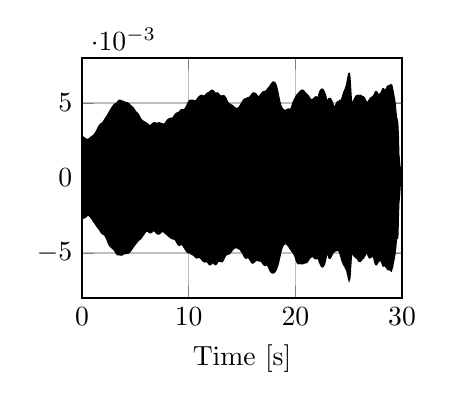
\begin{tikzpicture}
\begin{axis}[%
width=1.6in,
height=1.2in,
at={(0.758in,0.481in)},
scale only axis,
xmin=0,
xmax=30,
xmajorgrids,
ymin=-0.008,
ymax=0.008,
ymajorgrids,
xlabel={Time [s]},
axis background/.style={fill=white}
]
\addplot[fill=black,draw=black,forget plot] plot table[row sep=crcr]{%
2.08333333333333e-05	0.00308632850646973\\
0.0417454218822439	0.00275671482086182\\
0.0834700104311544	0.00273704528808594\\
0.125194598980065	0.00272452831268311\\
0.166919187528975	0.00270450115203857\\
0.208643776077886	0.00268077850341797\\
0.250368364626797	0.00264525413513184\\
0.292092953175707	0.00263023376464844\\
0.333817541724618	0.00261020660400391\\
0.375542130273528	0.00259864330291748\\
0.417266718822439	0.00258278846740723\\
0.458991307371349	0.00258219242095947\\
0.50071589592026	0.00257980823516846\\
0.54244048446917	0.00257468223571777\\
0.584165073018081	0.00259733200073242\\
0.625889661566991	0.00260865688323975\\
0.667614250115902	0.00262689590454102\\
0.709338838664812	0.002632737159729\\
0.751063427213723	0.00266110897064209\\
0.792788015762633	0.00269877910614014\\
0.834512604311544	0.00272214412689209\\
0.876237192860454	0.00275874137878418\\
0.917961781409365	0.00276803970336914\\
0.959686369958275	0.00279343128204346\\
1.00141095850719	0.00279641151428223\\
1.0431355470561	0.00283312797546387\\
1.08486013560501	0.00285840034484863\\
1.12658472415392	0.00288236141204834\\
1.16830931270283	0.00293529033660889\\
1.21003390125174	0.00296568870544434\\
1.25175848980065	0.00302159786224365\\
1.29348307834956	0.00306785106658936\\
1.33520766689847	0.00311791896820068\\
1.37693225544738	0.00316596031188965\\
1.41865684399629	0.00323522090911865\\
1.4603814325452	0.0032966136932373\\
1.50210602109411	0.00336408615112305\\
1.54383060964302	0.00341379642486572\\
1.58555519819193	0.00346755981445313\\
1.62727978674084	0.0035092830657959\\
1.66900437528975	0.00354480743408203\\
1.71072896383866	0.00356411933898926\\
1.75245355238758	0.00359487533569336\\
1.79417814093649	0.00363492965698242\\
1.8359027294854	0.00363993644714355\\
1.87762731803431	0.00365757942199707\\
1.91935190658322	0.00368618965148926\\
1.96107649513213	0.00373387336730957\\
2.00280108368104	0.00377106666564941\\
2.04452567222995	0.00380182266235352\\
2.08625026077886	0.00385951995849609\\
2.12797484932777	0.00392401218414307\\
2.16969943787668	0.00396168231964111\\
2.21142402642559	0.0039975643157959\\
2.2531486149745	0.004050612449646\\
2.29487320352341	0.00408756732940674\\
2.33659779207232	0.00414228439331055\\
2.37832238062123	0.00418353080749512\\
2.42004696917014	0.00424253940582275\\
2.46177155771905	0.00428080558776855\\
2.50349614626796	0.00433754920959473\\
2.54522073481687	0.0043947696685791\\
2.58694532336579	0.00444936752319336\\
2.6286699119147	0.00449645519256592\\
2.67039450046361	0.00455117225646973\\
2.71211908901252	0.00458920001983643\\
2.75384367756143	0.00465130805969238\\
2.79556826611034	0.00470423698425293\\
2.83729285465925	0.00473761558532715\\
2.87901744320816	0.00477850437164307\\
2.92074203175707	0.00481486320495605\\
2.96246662030598	0.00485944747924805\\
3.00419120885489	0.00489699840545654\\
3.0459157974038	0.00491297245025635\\
3.08764038595271	0.00493454933166504\\
3.12936497450162	0.0049588680267334\\
3.17108956305053	0.00496351718902588\\
3.21281415159944	0.00497102737426758\\
3.25453874014835	0.00501096248626709\\
3.29626332869726	0.00502884387969971\\
3.33798791724618	0.00508403778076172\\
3.37971250579509	0.005118727684021\\
3.421437094344	0.00516402721405029\\
3.46316168289291	0.00516963005065918\\
3.50488627144182	0.0051800012588501\\
3.54661085999073	0.00518536567687988\\
3.58833544853964	0.00517785549163818\\
3.63006003708855	0.0051581859588623\\
3.67178462563746	0.00515079498291016\\
3.71350921418637	0.00513231754302979\\
3.75523380273528	0.00512814521789551\\
3.79695839128419	0.00511276721954346\\
3.8386829798331	0.0051114559173584\\
3.88040756838201	0.00510227680206299\\
3.92213215693092	0.00507569313049316\\
3.96385674547983	0.00507783889770508\\
4.00558133402874	0.00505614280700684\\
4.04730592257765	0.0050431489944458\\
4.08903051112656	0.00503849983215332\\
4.13075509967547	0.00502896308898926\\
4.17247968822439	0.00502562522888184\\
4.2142042767733	0.00500881671905518\\
4.25592886532221	0.00501561164855957\\
4.29765345387112	0.0049896240234375\\
4.33937804242003	0.00498640537261963\\
4.38110263096894	0.00496840476989746\\
4.42282721951785	0.00494635105133057\\
4.46455180806676	0.00490283966064453\\
4.50627639661567	0.0048677921295166\\
4.54800098516458	0.00484287738800049\\
4.58972557371349	0.00480782985687256\\
4.6314501622624	0.00479269027709961\\
4.67317475081131	0.00475978851318359\\
4.71489933936022	0.0047307014465332\\
4.75662392790913	0.00471353530883789\\
4.79834851645804	0.00467085838317871\\
4.84007310500695	0.00463080406188965\\
4.88179769355586	0.00459074974060059\\
4.92352228210478	0.00454413890838623\\
4.96524687065368	0.00450289249420166\\
5.0069714592026	0.00444686412811279\\
5.04869604775151	0.00441312789916992\\
5.09042063630042	0.00439107418060303\\
5.13214522484933	0.00436878204345703\\
5.17386981339824	0.00434136390686035\\
5.21559440194715	0.00430750846862793\\
5.25731899049606	0.00427210330963135\\
5.29904357904497	0.00422859191894531\\
5.34076816759388	0.00417828559875488\\
5.38249275614279	0.00411856174468994\\
5.4242173446917	0.00406348705291748\\
5.46594193324061	0.00400161743164063\\
5.50766652178952	0.00394546985626221\\
5.54939111033843	0.00389492511749268\\
5.59111569888734	0.00387120246887207\\
5.63284028743625	0.00384151935577393\\
5.67456487598516	0.00382614135742188\\
5.71628946453407	0.00379598140716553\\
5.75801405308299	0.00377225875854492\\
5.7997386416319	0.0037529468536377\\
5.84146323018081	0.00373804569244385\\
5.88318781872972	0.00371789932250977\\
5.92491240727863	0.00371134281158447\\
5.96663699582754	0.00369918346405029\\
6.00836158437645	0.00368452072143555\\
6.05008617292536	0.00365674495697021\\
6.09181076147427	0.00364029407501221\\
6.13353535002318	0.00361907482147217\\
6.17525993857209	0.00358903408050537\\
6.216984527121	0.0035407543182373\\
6.25870911566991	0.00352931022644043\\
6.30043370421882	0.00351178646087646\\
6.34215829276773	0.00350403785705566\\
6.38388288131664	0.00351357460021973\\
6.42560746986555	0.00351905822753906\\
6.46733205841446	0.00354361534118652\\
6.50905664696338	0.00356996059417725\\
6.55078123551229	0.00359165668487549\\
6.5925058240612	0.00361359119415283\\
6.63423041261011	0.00364196300506592\\
6.67595500115902	0.00367200374603271\\
6.71767958970793	0.00367748737335205\\
6.75940417825684	0.00368714332580566\\
6.80112876680575	0.00368881225585938\\
6.84285335535466	0.00367629528045654\\
6.88457794390357	0.0036691427230835\\
6.92630253245248	0.00365746021270752\\
6.96802712100139	0.00364530086517334\\
7.0097517095503	0.00364530086517334\\
7.05147629809921	0.00364792346954346\\
7.09320088664812	0.00365746021270752\\
7.13492547519703	0.0036766529083252\\
7.17665006374594	0.00368213653564453\\
7.21837465229485	0.00368416309356689\\
7.26009924084376	0.00366842746734619\\
7.30182382939268	0.00366783142089844\\
7.34354841794159	0.00365209579467773\\
7.3852730064905	0.0036461353302002\\
7.42699759503941	0.00363492965698242\\
7.46872218358832	0.00362944602966309\\
7.51044677213723	0.0036090612411499\\
7.55217136068614	0.00361084938049316\\
7.59389594923505	0.00359237194061279\\
7.63562053778396	0.00358748435974121\\
7.67734512633287	0.00359702110290527\\
7.71906971488178	0.0036083459854126\\
7.76079430343069	0.00363409519195557\\
7.8025188919796	0.00366663932800293\\
7.84424348052851	0.00370883941650391\\
7.88596806907742	0.00375974178314209\\
7.92769265762633	0.00379693508148193\\
7.96941724617524	0.00383603572845459\\
8.01114183472416	0.00386989116668701\\
8.05286642327307	0.0038989782333374\\
8.09459101182198	0.00391614437103271\\
8.13631560037089	0.00394165515899658\\
8.1780401889198	0.00394999980926514\\
8.21976477746871	0.00397217273712158\\
8.26148936601762	0.00397574901580811\\
8.30321395456653	0.00398588180541992\\
8.34493854311544	0.00398123264312744\\
8.38666313166435	0.00398123264312744\\
8.42838772021326	0.003989577293396\\
8.47011230876217	0.0039980411529541\\
8.51183689731108	0.00402176380157471\\
8.55356148585999	0.00405430793762207\\
8.5952860744089	0.00410354137420654\\
8.63701066295781	0.00414609909057617\\
8.67873525150672	0.00419330596923828\\
8.72045984005563	0.0042191743850708\\
8.76218442860454	0.00426948070526123\\
8.80390901715345	0.00429034233093262\\
8.84563360570237	0.00430834293365479\\
8.88735819425128	0.00432348251342773\\
8.92908278280018	0.00435173511505127\\
8.9708073713491	0.00435888767242432\\
9.01253195989801	0.00437009334564209\\
9.05425654844692	0.00438380241394043\\
9.09598113699583	0.0043952465057373\\
9.13770572554474	0.00443148612976074\\
9.17943031409365	0.00446403026580811\\
9.22115490264256	0.00450325012207031\\
9.26287949119147	0.00452744960784912\\
9.30460407974038	0.00455212593078613\\
9.34632866828929	0.00455951690673828\\
9.3880532568382	0.00457000732421875\\
9.42977784538711	0.00456917285919189\\
9.47150243393602	0.0045623779296875\\
9.51322702248493	0.00455796718597412\\
9.55495161103384	0.00455951690673828\\
9.59667619958275	0.00457537174224854\\
9.63840078813166	0.00461328029632568\\
9.68012537668058	0.00464427471160889\\
9.72184996522949	0.0046992301940918\\
9.7635745537784	0.0047382116317749\\
9.80529914232731	0.00481772422790527\\
9.84702373087622	0.00486540794372559\\
9.88874831942513	0.00493884086608887\\
9.93047290797404	0.00500059127807617\\
9.97219749652295	0.00505650043487549\\
10.0139220850719	0.00511908531188965\\
10.0556466736208	0.00514781475067139\\
10.0973712621697	0.00517666339874268\\
10.1390958507186	0.00518953800201416\\
10.1808204392675	0.00518798828125\\
10.2225450278164	0.00518405437469482\\
10.2642696163653	0.00518655776977539\\
10.3059942049142	0.00517952442169189\\
10.3477187934631	0.00518620014190674\\
10.3894433820121	0.00518333911895752\\
10.431167970561	0.00517916679382324\\
10.4728925591099	0.00516331195831299\\
10.5146171476588	0.00515449047088623\\
10.5563417362077	0.00514280796051025\\
10.5980663247566	0.00513374805450439\\
10.6397909133055	0.00514411926269531\\
10.6815155018544	0.00517570972442627\\
10.7232400904033	0.00519120693206787\\
10.7649646789523	0.00522327423095703\\
10.8066892675012	0.0052725076675415\\
10.8484138560501	0.00532174110412598\\
10.890138444599	0.00535178184509277\\
10.9318630331479	0.00539648532867432\\
10.9735876216968	0.00543022155761719\\
11.0153122102457	0.00545752048492432\\
11.0570367987946	0.00546836853027344\\
11.0987613873435	0.00547921657562256\\
11.1404859758924	0.00549089908599854\\
11.1822105644414	0.00551366806030273\\
11.2239351529903	0.00550377368927002\\
11.2656597415392	0.00549781322479248\\
11.3073843300881	0.00548040866851807\\
11.349108918637	0.00547695159912109\\
11.3908335071859	0.00546705722808838\\
11.4325580957348	0.00546860694885254\\
11.4742826842837	0.00547111034393311\\
11.5160072728326	0.00549209117889404\\
11.5577318613816	0.00551784038543701\\
11.5994564499305	0.00555181503295898\\
11.6411810384794	0.00558269023895264\\
11.6829056270283	0.00562310218811035\\
11.7246302155772	0.00564360618591309\\
11.7663548041261	0.00566446781158447\\
11.808079392675	0.00568866729736328\\
11.8498039812239	0.00570273399353027\\
11.8915285697728	0.00570809841156006\\
11.9332531583217	0.00572574138641357\\
11.9749777468707	0.00575315952301025\\
12.0167023354196	0.00576150417327881\\
12.0584269239685	0.00578951835632324\\
12.1001515125174	0.00582242012023926\\
12.1418761010663	0.00583994388580322\\
12.1836006896152	0.00584709644317627\\
12.2253252781641	0.00584876537322998\\
12.267049866713	0.00583720207214355\\
12.3087744552619	0.00581240653991699\\
12.3504990438108	0.00577032566070557\\
12.3922236323598	0.00573611259460449\\
12.4339482209087	0.00571310520172119\\
12.4756728094576	0.00566554069519043\\
12.5173973980065	0.00565183162689209\\
12.5591219865554	0.00566184520721436\\
12.6008465751043	0.00566232204437256\\
12.6425711636532	0.00566887855529785\\
12.6842957522021	0.00567686557769775\\
12.726020340751	0.00567054748535156\\
12.7677449293	0.00564432144165039\\
12.8094695178489	0.00561010837554932\\
12.8511941063978	0.00557601451873779\\
12.8929186949467	0.00552880764007568\\
12.9346432834956	0.00549697875976563\\
12.9763678720445	0.00549042224884033\\
13.0180924605934	0.00547003746032715\\
13.0598170491423	0.00546002388000488\\
13.1015416376912	0.00546109676361084\\
13.1432662262401	0.0054624080657959\\
13.1849908147891	0.00548458099365234\\
13.226715403338	0.00549173355102539\\
13.2684399918869	0.00549113750457764\\
13.3101645804358	0.00548195838928223\\
13.3518891689847	0.00545275211334229\\
13.3936137575336	0.00541269779205322\\
13.4353383460825	0.00538945198059082\\
13.4770629346314	0.00532805919647217\\
13.5187875231803	0.00528335571289063\\
13.5605121117293	0.00519800186157227\\
13.6022367002782	0.00513482093811035\\
13.6439612888271	0.0050889253616333\\
13.685685877376	0.00503551959991455\\
13.7274104659249	0.00500345230102539\\
13.7691350544738	0.00496459007263184\\
13.8108596430227	0.00495541095733643\\
13.8525842315716	0.00493049621582031\\
13.8943088201205	0.00491511821746826\\
13.9360334086694	0.00489175319671631\\
13.9777579972184	0.00487160682678223\\
14.0194825857673	0.00486171245574951\\
14.0612071743162	0.00484192371368408\\
14.1029317628651	0.00483667850494385\\
14.144656351414	0.00480687618255615\\
14.1863809399629	0.00478100776672363\\
14.2281055285118	0.00475645065307617\\
14.2698301170607	0.00471687316894531\\
14.3115547056096	0.00470590591430664\\
14.3532792941586	0.00467395782470703\\
14.3950038827075	0.00466561317443848\\
14.4367284712564	0.00465750694274902\\
14.4784530598053	0.00465714931488037\\
14.5201776483542	0.00465011596679688\\
14.5619022369031	0.00464797019958496\\
14.603626825452	0.0046546459197998\\
14.6453514140009	0.00465977191925049\\
14.6870760025498	0.0046926736831665\\
14.7288005910988	0.00472903251647949\\
14.7705251796477	0.0047764778137207\\
14.8122497681966	0.00481688976287842\\
14.8539743567455	0.00486946105957031\\
14.8956989452944	0.00491881370544434\\
14.9374235338433	0.00497043132781982\\
14.9791481223922	0.00502347946166992\\
15.0208727109411	0.00507235527038574\\
15.06259729949	0.00511407852172852\\
15.1043218880389	0.00516796112060547\\
15.1460464765879	0.00521492958068848\\
15.1877710651368	0.00524377822875977\\
15.2294956536857	0.00525975227355957\\
15.2712202422346	0.00528013706207275\\
15.3129448307835	0.00528895854949951\\
15.3546694193324	0.00529885292053223\\
15.3963940078813	0.00529015064239502\\
15.4381185964302	0.0053175687789917\\
15.4798431849791	0.00531435012817383\\
15.521567773528	0.00535154342651367\\
15.563292362077	0.00534474849700928\\
15.6050169506259	0.00536489486694336\\
15.6467415391748	0.00537025928497314\\
15.6884661277237	0.0053868293762207\\
15.7301907162726	0.00541079044342041\\
15.7719153048215	0.00541913509368896\\
15.8136398933704	0.00549459457397461\\
15.8553644819193	0.00550329685211182\\
15.8970890704682	0.00557005405426025\\
15.9388136590172	0.00560343265533447\\
15.9805382475661	0.00562524795532227\\
16.022262836115	0.00565862655639648\\
16.0639874246639	0.00564718246459961\\
16.1057120132128	0.00567317008972168\\
16.1474366017617	0.00566184520721436\\
16.1891611903106	0.00565934181213379\\
16.2308857788595	0.00564813613891602\\
16.2726103674084	0.00561094284057617\\
16.3143349559573	0.00560963153839111\\
16.3560595445063	0.00553381443023682\\
16.3977841330552	0.00551915168762207\\
16.4395087216041	0.00547587871551514\\
16.481233310153	0.0054466724395752\\
16.5229578987019	0.00543487071990967\\
16.5646824872508	0.00543749332427979\\
16.6064070757997	0.00544369220733643\\
16.6481316643486	0.00545787811279297\\
16.6898562528975	0.00550544261932373\\
16.7315808414465	0.00554466247558594\\
16.7733054299954	0.00560545921325684\\
16.8150300185443	0.00562179088592529\\
16.8567546070932	0.00566434860229492\\
16.8984791956421	0.00567734241485596\\
16.940203784191	0.00572896003723145\\
16.9819283727399	0.00573074817657471\\
17.0236529612888	0.00574445724487305\\
17.0653775498377	0.00576698780059814\\
17.1071021383867	0.00575363636016846\\
17.1488267269356	0.00578033924102783\\
17.1905513154845	0.00576627254486084\\
17.2322759040334	0.00579571723937988\\
17.2740004925823	0.0058213472366333\\
17.3157250811312	0.00585556030273438\\
17.3574496696801	0.00589728355407715\\
17.399174258229	0.00596058368682861\\
17.4408988467779	0.00597572326660156\\
17.4826234353268	0.00602567195892334\\
17.5243480238758	0.00605869293212891\\
17.5660726124247	0.00609612464904785\\
17.6077972009736	0.00612449645996094\\
17.6495217895225	0.00617122650146484\\
17.6912463780714	0.00622260570526123\\
17.7329709666203	0.00626766681671143\\
17.7746955551692	0.00630152225494385\\
17.8164201437181	0.00633704662322998\\
17.858144732267	0.00638163089752197\\
17.8998693208159	0.00639796257019043\\
17.9415939093649	0.00640380382537842\\
17.9833184979138	0.00639247894287109\\
18.0250430864627	0.00638711452484131\\
18.0667676750116	0.00635731220245361\\
18.1084922635605	0.00632107257843018\\
18.1502168521094	0.0062793493270874\\
18.1919414406583	0.00620102882385254\\
18.2336660292072	0.00612878799438477\\
18.2753906177561	0.00601112842559814\\
18.3171152063051	0.00587248802185059\\
18.358839794854	0.00574111938476563\\
18.4005643834029	0.00559806823730469\\
18.4422889719518	0.00544750690460205\\
18.4840135605007	0.00529384613037109\\
18.5257381490496	0.00515162944793701\\
18.5674627375985	0.00502979755401611\\
18.6091873261474	0.00492668151855469\\
18.6509119146963	0.00483250617980957\\
18.6926365032453	0.0047457218170166\\
18.7343610917942	0.00468885898590088\\
18.7760856803431	0.00464475154876709\\
18.817810268892	0.00460135936737061\\
18.8595348574409	0.00457251071929932\\
18.9012594459898	0.00455152988433838\\
18.9429840345387	0.00452113151550293\\
18.9847086230876	0.00451076030731201\\
19.0264332116365	0.00451040267944336\\
19.0681578001854	0.00451147556304932\\
19.1098823887344	0.00451791286468506\\
19.1516069772833	0.00454866886138916\\
19.1933315658322	0.00455200672149658\\
19.2350561543811	0.00456655025482178\\
19.27678074293	0.00458920001983643\\
19.3185053314789	0.00459706783294678\\
19.3602299200278	0.00460660457611084\\
19.4019545085767	0.00459909439086914\\
19.4436790971256	0.00457131862640381\\
19.4854036856745	0.00457537174224854\\
19.5271282742235	0.00457370281219482\\
19.5688528627724	0.00461244583129883\\
19.6105774513213	0.00467753410339355\\
19.6523020398702	0.00476658344268799\\
19.6940266284191	0.00484573841094971\\
19.735751216968	0.00493419170379639\\
19.7774758055169	0.00503635406494141\\
19.8192003940658	0.00509440898895264\\
19.8609249826147	0.00517213344573975\\
19.9026495711637	0.00521242618560791\\
19.9443741597126	0.00528895854949951\\
19.9860987482615	0.00533640384674072\\
20.0278233368104	0.0054011344909668\\
20.0695479253593	0.00544321537017822\\
20.1112725139082	0.00551712512969971\\
20.1529971024571	0.00553429126739502\\
20.194721691006	0.0055854320526123\\
20.2364462795549	0.00560271739959717\\
20.2781708681038	0.00563728809356689\\
20.3198954566528	0.00566315650939941\\
20.3616200452017	0.00570392608642578\\
20.4033446337506	0.00574362277984619\\
20.4450692222995	0.00578165054321289\\
20.4867938108484	0.00579166412353516\\
20.5285183993973	0.00582671165466309\\
20.5702429879462	0.00585496425628662\\
20.6119675764951	0.00583922863006592\\
20.653692165044	0.00585711002349854\\
20.695416753593	0.00584208965301514\\
20.7371413421419	0.00584506988525391\\
20.7788659306908	0.00581824779510498\\
20.8205905192397	0.00577080249786377\\
20.8623151077886	0.0057520866394043\\
20.9040396963375	0.00571310520172119\\
20.9457642848864	0.00567352771759033\\
20.9874888734353	0.0056452751159668\\
21.0292134619842	0.0055997371673584\\
21.0709380505331	0.00558769702911377\\
21.1126626390821	0.00556433200836182\\
21.154387227631	0.00553011894226074\\
21.1961118161799	0.00550532341003418\\
21.2378364047288	0.00543415546417236\\
21.2795609932777	0.00542163848876953\\
21.3212855818266	0.0053476095199585\\
21.3630101703755	0.00532984733581543\\
21.4047347589244	0.0052647590637207\\
21.4464593474733	0.00525331497192383\\
21.4881839360223	0.00522720813751221\\
21.5299085245712	0.0052337646484375\\
21.5716331131201	0.00522994995117188\\
21.613357701669	0.00525796413421631\\
21.6550822902179	0.00525665283203125\\
21.6968068787668	0.0052868127822876\\
21.7385314673157	0.00532007217407227\\
21.7802560558646	0.00534486770629883\\
21.8219806444135	0.00537014007568359\\
21.8637052329624	0.00538158416748047\\
21.9054298215114	0.00541532039642334\\
21.9471544100603	0.00541818141937256\\
21.9888789986092	0.00538194179534912\\
22.0306035871581	0.00537395477294922\\
22.072328175707	0.00534939765930176\\
22.1140527642559	0.00535988807678223\\
22.1557773528048	0.00545608997344971\\
22.1975019413537	0.00559377670288086\\
22.2392265299026	0.00565028190612793\\
22.2809511184516	0.00574111938476563\\
22.3226757070005	0.00581371784210205\\
22.3644002955494	0.00584924221038818\\
22.4061248840983	0.00589835643768311\\
22.4478494726472	0.00590431690216064\\
22.4895740611961	0.00593221187591553\\
22.531298649745	0.00592482089996338\\
22.5730232382939	0.0059058666229248\\
22.6147478268428	0.00586557388305664\\
22.6564724153917	0.0058358907699585\\
22.6981970039407	0.00576949119567871\\
22.7399215924896	0.00567865371704102\\
22.7816461810385	0.0056302547454834\\
22.8233707695874	0.00551462173461914\\
22.8650953581363	0.00543487071990967\\
22.9068199466852	0.00529253482818604\\
22.9485445352341	0.00520002841949463\\
22.990269123783	0.00510537624359131\\
23.0319937123319	0.00511729717254639\\
23.0737183008809	0.00519132614135742\\
23.1154428894298	0.00528228282928467\\
23.1571674779787	0.00529766082763672\\
23.1988920665276	0.00529229640960693\\
23.2406166550765	0.00530552864074707\\
23.2823412436254	0.0052722692489624\\
23.3240658321743	0.00527596473693848\\
23.3657904207232	0.00518298149108887\\
23.4075150092721	0.0051732063293457\\
23.449239597821	0.00506055355072021\\
23.49096418637	0.00500690937042236\\
23.5326887749189	0.00490212440490723\\
23.5744133634678	0.00482988357543945\\
23.6161379520167	0.00476980209350586\\
23.6578625405656	0.00474059581756592\\
23.6995871291145	0.00475442409515381\\
23.7413117176634	0.00480937957763672\\
23.7830363062123	0.0048677921295166\\
23.8247608947612	0.00493967533111572\\
23.8664854833102	0.00498104095458984\\
23.9082100718591	0.00504648685455322\\
23.949934660408	0.00505971908569336\\
23.9916592489569	0.00510406494140625\\
24.0333838375058	0.00511622428894043\\
24.0751084260547	0.00512123107910156\\
24.1168330146036	0.00511455535888672\\
24.1585576031525	0.00516831874847412\\
24.2002821917014	0.00514578819274902\\
24.2420067802503	0.00516796112060547\\
24.2837313687993	0.00520074367523193\\
24.3254559573482	0.00522375106811523\\
24.3671805458971	0.005340576171875\\
24.408905134446	0.00539231300354004\\
24.4506297229949	0.00555217266082764\\
24.4923543115438	0.00555849075317383\\
24.5340789000927	0.0057297945022583\\
24.5758034886416	0.00573873519897461\\
24.6175280771905	0.00586163997650146\\
24.6592526657395	0.00592339038848877\\
24.7009772542884	0.00601065158843994\\
24.7427018428373	0.00610709190368652\\
24.7844264313862	0.00617718696594238\\
24.8261510199351	0.00635647773742676\\
24.867875608484	0.00650680065155029\\
24.9096001970329	0.00667083263397217\\
24.9513247855818	0.00681221485137939\\
24.9930493741307	0.00696480274200439\\
25.0347739626796	0.00696825981140137\\
25.0764985512286	0.00697624683380127\\
25.1182231397775	0.00673246383666992\\
25.1599477283264	0.0063549280166626\\
25.2016723168753	0.0057908296585083\\
25.2433969054242	0.00533509254455566\\
25.2851214939731	0.00503969192504883\\
25.326846082522	0.00493299961090088\\
25.3685706710709	0.00500309467315674\\
25.4102952596198	0.00511455535888672\\
25.4520198481687	0.00512409210205078\\
25.4937444367177	0.00521671772003174\\
25.5354690252666	0.005271315574646\\
25.5771936138155	0.00534677505493164\\
25.6189182023644	0.00539577007293701\\
25.6606427909133	0.00541698932647705\\
25.7023673794622	0.00548171997070313\\
25.7440919680111	0.00547420978546143\\
25.78581655656	0.00548374652862549\\
25.8275411451089	0.00550544261932373\\
25.8692657336579	0.00551509857177734\\
25.9109903222068	0.00551116466522217\\
25.9527149107557	0.0055159330368042\\
25.9944394993046	0.00549411773681641\\
26.0361640878535	0.00549447536468506\\
26.0778886764024	0.00550508499145508\\
26.1196132649513	0.00551128387451172\\
26.1613378535002	0.00549530982971191\\
26.2030624420491	0.00546169281005859\\
26.2447870305981	0.00544869899749756\\
26.286511619147	0.00543153285980225\\
26.3282362076959	0.00542199611663818\\
26.3699607962448	0.00541400909423828\\
26.4116853847937	0.00538480281829834\\
26.4534099733426	0.00535321235656738\\
26.4951345618915	0.00532341003417969\\
26.5368591504404	0.00525999069213867\\
26.5785837389893	0.00519466400146484\\
26.6203083275383	0.00512731075286865\\
26.6620329160872	0.00506699085235596\\
26.7037575046361	0.0050656795501709\\
26.745482093185	0.0050361156463623\\
26.7872066817339	0.00505733489990234\\
26.8289312702828	0.00510323047637939\\
26.8706558588317	0.00513875484466553\\
26.9123804473806	0.00520801544189453\\
26.9541050359295	0.00522494316101074\\
26.9958296244784	0.00528228282928467\\
27.0375542130274	0.00533425807952881\\
27.0792788015763	0.00535738468170166\\
27.1210033901252	0.00537276268005371\\
27.1627279786741	0.00538694858551025\\
27.204452567223	0.00540411472320557\\
27.2461771557719	0.00539684295654297\\
27.2879017443208	0.00546443462371826\\
27.3296263328697	0.00549924373626709\\
27.3713509214186	0.00553786754608154\\
27.4130755099675	0.00558936595916748\\
27.4548000985165	0.0056920051574707\\
27.4965246870654	0.00572288036346436\\
27.5382492756143	0.00576412677764893\\
27.5799738641632	0.00576293468475342\\
27.6216984527121	0.00573611259460449\\
27.663423041261	0.00571072101593018\\
27.7051476298099	0.00565934181213379\\
27.7468722183588	0.00559043884277344\\
27.7885968069077	0.00558602809906006\\
27.8303213954567	0.00559186935424805\\
27.8720459840056	0.00559461116790771\\
27.9137705725545	0.00557887554168701\\
27.9554951611034	0.00557100772857666\\
27.9972197496523	0.00564026832580566\\
28.0389443382012	0.00571274757385254\\
28.0806689267501	0.00575315952301025\\
28.122393515299	0.00583136081695557\\
28.1641181038479	0.00591480731964111\\
28.2058426923968	0.00595808029174805\\
28.2475672809458	0.00596606731414795\\
28.2892918694947	0.00593388080596924\\
28.3310164580436	0.00589346885681152\\
28.3727410465925	0.00586497783660889\\
28.4144656351414	0.00586259365081787\\
28.4561902236903	0.00588667392730713\\
28.4979148122392	0.00593304634094238\\
28.5396394007881	0.00594735145568848\\
28.581363989337	0.00603437423706055\\
28.623088577886	0.00610876083374023\\
28.6648131664349	0.00612616539001465\\
28.7065377549838	0.00613009929656982\\
28.7482623435327	0.00614595413208008\\
28.7899869320816	0.00615668296813965\\
28.8317115206305	0.00617349147796631\\
28.8734361091794	0.00617456436157227\\
28.9151606977283	0.00620937347412109\\
28.9568852862772	0.00623774528503418\\
28.9986098748261	0.00619542598724365\\
29.0403344633751	0.00618624687194824\\
29.082059051924	0.00606787204742432\\
29.1237836404729	0.00591051578521729\\
29.1655082290218	0.00578665733337402\\
29.2072328175707	0.00561273097991943\\
29.2489574061196	0.00545871257781982\\
29.2906819946685	0.00531399250030518\\
29.3324065832174	0.00511109828948975\\
29.3741311717663	0.00487542152404785\\
29.4158557603153	0.0045241117477417\\
29.4575803488642	0.00423872470855713\\
29.4993049374131	0.00400471687316895\\
29.541029525962	0.00389373302459717\\
29.5827541145109	0.00382602214813232\\
29.6244787030598	0.00340914726257324\\
29.6662032916087	0.00269246101379395\\
29.7079278801576	0.00153839588165283\\
29.7496524687065	0.0012667179107666\\
29.7913770572554	0.000874996185302734\\
29.8331016458044	0.000686049461364746\\
29.8748262343533	0.000517487525939941\\
29.9165508229022	0.000445723533630371\\
29.9582754114511	0.000267505645751953\\
30	0.000217080116271973\\
}
\closedcycle;
\addplot[fill=black,draw=black,forget plot] plot table[row sep=crcr]{%
2.08333333333333e-05	-0.0033717155456543\\
0.0417454218822439	-0.00271034240722656\\
0.0834700104311544	-0.00268185138702393\\
0.125194598980065	-0.00267434120178223\\
0.166919187528975	-0.00267434120178223\\
0.208643776077886	-0.00266182422637939\\
0.250368364626797	-0.00265645980834961\\
0.292092953175707	-0.00264143943786621\\
0.333817541724618	-0.00262486934661865\\
0.375542130273528	-0.0025864839553833\\
0.417266718822439	-0.00256967544555664\\
0.458991307371349	-0.00252711772918701\\
0.50071589592026	-0.00252246856689453\\
0.54244048446917	-0.00250470638275146\\
0.584165073018081	-0.00249338150024414\\
0.625889661566991	-0.00251007080078125\\
0.667614250115902	-0.0025249719619751\\
0.709338838664812	-0.00255715847015381\\
0.751063427213723	-0.00258517265319824\\
0.792788015762633	-0.00261092185974121\\
0.834512604311544	-0.00266098976135254\\
0.876237192860454	-0.00268650054931641\\
0.917961781409365	-0.00273418426513672\\
0.959686369958275	-0.00276505947113037\\
1.00141095850719	-0.00282967090606689\\
1.0431355470561	-0.0028688907623291\\
1.08486013560501	-0.00292050838470459\\
1.12658472415392	-0.00295937061309814\\
1.16830931270283	-0.00300157070159912\\
1.21003390125174	-0.00305032730102539\\
1.25175848980065	-0.00308382511138916\\
1.29348307834956	-0.00313472747802734\\
1.33520766689847	-0.00317180156707764\\
1.37693225544738	-0.00322890281677246\\
1.41865684399629	-0.00325191020965576\\
1.4603814325452	-0.00330185890197754\\
1.50210602109411	-0.0033419132232666\\
1.54383060964302	-0.0033794641494751\\
1.58555519819193	-0.0034104585647583\\
1.62727978674084	-0.00345098972320557\\
1.66900437528975	-0.00350391864776611\\
1.71072896383866	-0.00355350971221924\\
1.75245355238758	-0.00359892845153809\\
1.79417814093649	-0.00364148616790771\\
1.8359027294854	-0.00368237495422363\\
1.87762731803431	-0.00369870662689209\\
1.91935190658322	-0.00372040271759033\\
1.96107649513213	-0.00374674797058105\\
2.00280108368104	-0.00376307964324951\\
2.04452567222995	-0.00378429889678955\\
2.08625026077886	-0.00380980968475342\\
2.12797484932777	-0.00384318828582764\\
2.16969943787668	-0.00387609004974365\\
2.21142402642559	-0.00393438339233398\\
2.2531486149745	-0.00399541854858398\\
2.29487320352341	-0.00406014919281006\\
2.33659779207232	-0.0041271448135376\\
2.37832238062123	-0.0042111873626709\\
2.42004696917014	-0.0042870044708252\\
2.46177155771905	-0.00436556339263916\\
2.50349614626796	-0.00441229343414307\\
2.54522073481687	-0.00446844100952148\\
2.58694532336579	-0.00451862812042236\\
2.6286699119147	-0.00456917285919189\\
2.67039450046361	-0.00458335876464844\\
2.71211908901252	-0.00461173057556152\\
2.75384367756143	-0.00464832782745361\\
2.79556826611034	-0.00466513633728027\\
2.83729285465925	-0.00469100475311279\\
2.87901744320816	-0.00471925735473633\\
2.92074203175707	-0.00474894046783447\\
2.96246662030598	-0.00475943088531494\\
3.00419120885489	-0.00479114055633545\\
3.0459157974038	-0.00484311580657959\\
3.08764038595271	-0.00489330291748047\\
3.12936497450162	-0.00496137142181396\\
3.17108956305053	-0.00499749183654785\\
3.21281415159944	-0.00505852699279785\\
3.25453874014835	-0.00508260726928711\\
3.29626332869726	-0.00511276721954346\\
3.33798791724618	-0.00511860847473145\\
3.37971250579509	-0.00513195991516113\\
3.421437094344	-0.0051194429397583\\
3.46316168289291	-0.00512158870697021\\
3.50488627144182	-0.00512230396270752\\
3.54661085999073	-0.00512778759002686\\
3.58833544853964	-0.00514328479766846\\
3.63006003708855	-0.00514566898345947\\
3.67178462563746	-0.00514686107635498\\
3.71350921418637	-0.00514912605285645\\
3.75523380273528	-0.00513648986816406\\
3.79695839128419	-0.00512444972991943\\
3.8386829798331	-0.00510728359222412\\
3.88040756838201	-0.00508058071136475\\
3.92213215693092	-0.0050663948059082\\
3.96385674547983	-0.00504469871520996\\
4.00558133402874	-0.00504565238952637\\
4.04730592257765	-0.00505423545837402\\
4.08903051112656	-0.00503885746002197\\
4.13075509967547	-0.00504434108734131\\
4.17247968822439	-0.00504422187805176\\
4.2142042767733	-0.00503969192504883\\
4.25592886532221	-0.00502395629882813\\
4.29765345387112	-0.00502336025238037\\
4.33937804242003	-0.00500750541687012\\
4.38110263096894	-0.00499880313873291\\
4.42282721951785	-0.00497472286224365\\
4.46455180806676	-0.00495493412017822\\
4.50627639661567	-0.00492382049560547\\
4.54800098516458	-0.00488400459289551\\
4.58972557371349	-0.00483870506286621\\
4.6314501622624	-0.00479686260223389\\
4.67317475081131	-0.00474929809570313\\
4.71489933936022	-0.00470292568206787\\
4.75662392790913	-0.00465047359466553\\
4.79834851645804	-0.00461411476135254\\
4.84007310500695	-0.00457251071929932\\
4.88179769355586	-0.0045323371887207\\
4.92352228210478	-0.00451743602752686\\
4.96524687065368	-0.00446689128875732\\
5.0069714592026	-0.00441348552703857\\
5.04869604775151	-0.00437963008880615\\
5.09042063630042	-0.004341721534729\\
5.13214522484933	-0.0043032169342041\\
5.17386981339824	-0.00426459312438965\\
5.21559440194715	-0.00423741340637207\\
5.25731899049606	-0.00420200824737549\\
5.29904357904497	-0.00416779518127441\\
5.34076816759388	-0.00414514541625977\\
5.38249275614279	-0.004128098487854\\
5.4242173446917	-0.00410020351409912\\
5.46594193324061	-0.00408005714416504\\
5.50766652178952	-0.00404214859008789\\
5.54939111033843	-0.00401175022125244\\
5.59111569888734	-0.00397002696990967\\
5.63284028743625	-0.00392818450927734\\
5.67456487598516	-0.00388145446777344\\
5.71628946453407	-0.0038381814956665\\
5.75801405308299	-0.00379633903503418\\
5.7997386416319	-0.00374877452850342\\
5.84146323018081	-0.00372958183288574\\
5.88318781872972	-0.00367486476898193\\
5.92491240727863	-0.00364315509796143\\
5.96663699582754	-0.0035930871963501\\
6.00836158437645	-0.00356853008270264\\
6.05008617292536	-0.00354897975921631\\
6.09181076147427	-0.00353765487670898\\
6.13353535002318	-0.00354683399200439\\
6.17525993857209	-0.00356769561767578\\
6.216984527121	-0.00358784198760986\\
6.25870911566991	-0.00361812114715576\\
6.30043370421882	-0.00363707542419434\\
6.34215829276773	-0.00365746021270752\\
6.38388288131664	-0.0036548376083374\\
6.42560746986555	-0.00366330146789551\\
6.46733205841446	-0.00365376472473145\\
6.50905664696338	-0.00363779067993164\\
6.55078123551229	-0.00361120700836182\\
6.5925058240612	-0.00358736515045166\\
6.63423041261011	-0.00355565547943115\\
6.67595500115902	-0.00353634357452393\\
6.71767958970793	-0.0035102367401123\\
6.75940417825684	-0.00351881980895996\\
6.80112876680575	-0.00354862213134766\\
6.84285335535466	-0.00357449054718018\\
6.88457794390357	-0.00361227989196777\\
6.92630253245248	-0.00365245342254639\\
6.96802712100139	-0.0036846399307251\\
7.0097517095503	-0.00370335578918457\\
7.05147629809921	-0.00372040271759033\\
7.09320088664812	-0.00374007225036621\\
7.13492547519703	-0.0037388801574707\\
7.17665006374594	-0.00373804569244385\\
7.21837465229485	-0.00373721122741699\\
7.26009924084376	-0.00372219085693359\\
7.30182382939268	-0.00370657444000244\\
7.34354841794159	-0.00368380546569824\\
7.3852730064905	-0.00364696979522705\\
7.42699759503941	-0.00362825393676758\\
7.46872218358832	-0.00359201431274414\\
7.51044677213723	-0.00357568264007568\\
7.55217136068614	-0.00356483459472656\\
7.59389594923505	-0.00357735157012939\\
7.63562053778396	-0.00359475612640381\\
7.67734512633287	-0.00361621379852295\\
7.71906971488178	-0.00365376472473145\\
7.76079430343069	-0.00366699695587158\\
7.8025188919796	-0.00369632244110107\\
7.84424348052851	-0.00373172760009766\\
7.88596806907742	-0.00375223159790039\\
7.92769265762633	-0.00377976894378662\\
7.96941724617524	-0.00379836559295654\\
8.01114183472416	-0.00382685661315918\\
8.05286642327307	-0.0038532018661499\\
8.09459101182198	-0.00387263298034668\\
8.13631560037089	-0.00389444828033447\\
8.1780401889198	-0.0039215087890625\\
8.21976477746871	-0.0039360523223877\\
8.26148936601762	-0.00397026538848877\\
8.30321395456653	-0.00398492813110352\\
8.34493854311544	-0.00401830673217773\\
8.38666313166435	-0.00403094291687012\\
8.42838772021326	-0.00404536724090576\\
8.47011230876217	-0.00406539440155029\\
8.51183689731108	-0.00406765937805176\\
8.55356148585999	-0.00407016277313232\\
8.5952860744089	-0.00406539440155029\\
8.63701066295781	-0.00408291816711426\\
8.67873525150672	-0.00408554077148438\\
8.72045984005563	-0.00412261486053467\\
8.76218442860454	-0.00415968894958496\\
8.80390901715345	-0.00420868396759033\\
8.84563360570237	-0.00426375865936279\\
8.88735819425128	-0.00431954860687256\\
8.92908278280018	-0.00437140464782715\\
8.9708073713491	-0.00441980361938477\\
9.01253195989801	-0.00445687770843506\\
9.05425654844692	-0.00447320938110352\\
9.09598113699583	-0.00449275970458984\\
9.13770572554474	-0.00448358058929443\\
9.17943031409365	-0.00447678565979004\\
9.22115490264256	-0.0044715404510498\\
9.26287949119147	-0.0044550895690918\\
9.30460407974038	-0.00444340705871582\\
9.34632866828929	-0.00444400310516357\\
9.3880532568382	-0.00445735454559326\\
9.42977784538711	-0.00447726249694824\\
9.47150243393602	-0.00453567504882813\\
9.51322702248493	-0.00457668304443359\\
9.55495161103384	-0.00463461875915527\\
9.59667619958275	-0.00468671321868896\\
9.63840078813166	-0.00473058223724365\\
9.68012537668058	-0.00478279590606689\\
9.72184996522949	-0.00481283664703369\\
9.7635745537784	-0.00487792491912842\\
9.80529914232731	-0.00489497184753418\\
9.84702373087622	-0.00494003295898438\\
9.88874831942513	-0.00496006011962891\\
9.93047290797404	-0.00498294830322266\\
9.97219749652295	-0.00498509407043457\\
10.0139220850719	-0.00500130653381348\\
10.0556466736208	-0.00499916076660156\\
10.0973712621697	-0.00500845909118652\\
10.1390958507186	-0.0050206184387207\\
10.1808204392675	-0.00504505634307861\\
10.2225450278164	-0.00507724285125732\\
10.2642696163653	-0.00508511066436768\\
10.3059942049142	-0.00510239601135254\\
10.3477187934631	-0.00512146949768066\\
10.3894433820121	-0.00513434410095215\\
10.431167970561	-0.00514233112335205\\
10.4728925591099	-0.0051645040512085\\
10.5146171476588	-0.00519585609436035\\
10.5563417362077	-0.00523257255554199\\
10.5980663247566	-0.00527679920196533\\
10.6397909133055	-0.00530135631561279\\
10.6815155018544	-0.00530707836151123\\
10.7232400904033	-0.00532674789428711\\
10.7649646789523	-0.00533938407897949\\
10.8066892675012	-0.00532126426696777\\
10.8484138560501	-0.00531208515167236\\
10.890138444599	-0.00530135631561279\\
10.9318630331479	-0.00530540943145752\\
10.9735876216968	-0.00530421733856201\\
11.0153122102457	-0.00531554222106934\\
11.0570367987946	-0.00533473491668701\\
11.0987613873435	-0.00535345077514648\\
11.1404859758924	-0.00537467002868652\\
11.1822105644414	-0.00540649890899658\\
11.2239351529903	-0.00543606281280518\\
11.2656597415392	-0.00548529624938965\\
11.3073843300881	-0.00551486015319824\\
11.349108918637	-0.00555157661437988\\
11.3908335071859	-0.00556957721710205\\
11.4325580957348	-0.00559329986572266\\
11.4742826842837	-0.00560557842254639\\
11.5160072728326	-0.00559711456298828\\
11.5577318613816	-0.00559413433074951\\
11.5994564499305	-0.00558757781982422\\
11.6411810384794	-0.00558972358703613\\
11.6829056270283	-0.00558221340179443\\
11.7246302155772	-0.00559341907501221\\
11.7663548041261	-0.00562834739685059\\
11.808079392675	-0.00566720962524414\\
11.8498039812239	-0.00569689273834229\\
11.8915285697728	-0.00574910640716553\\
11.9332531583217	-0.00576615333557129\\
11.9749777468707	-0.00578033924102783\\
12.0167023354196	-0.00579750537872314\\
12.0584269239685	-0.00578022003173828\\
12.1001515125174	-0.00576186180114746\\
12.1418761010663	-0.00572609901428223\\
12.1836006896152	-0.00569403171539307\\
12.2253252781641	-0.00566339492797852\\
12.267049866713	-0.00565254688262939\\
12.3087744552619	-0.00566518306732178\\
12.3504990438108	-0.00569677352905273\\
12.3922236323598	-0.00572896003723145\\
12.4339482209087	-0.00576817989349365\\
12.4756728094576	-0.00577831268310547\\
12.5173973980065	-0.00578582286834717\\
12.5591219865554	-0.00577187538146973\\
12.6008465751043	-0.00575077533721924\\
12.6425711636532	-0.00570511817932129\\
12.6842957522021	-0.00565147399902344\\
12.726020340751	-0.00559806823730469\\
12.7677449293	-0.00557076930999756\\
12.8094695178489	-0.00555288791656494\\
12.8511941063978	-0.00554490089416504\\
12.8929186949467	-0.00555825233459473\\
12.9346432834956	-0.0055471658706665\\
12.9763678720445	-0.00557327270507813\\
13.0180924605934	-0.00557470321655273\\
13.0598170491423	-0.00558996200561523\\
13.1015416376912	-0.00558876991271973\\
13.1432662262401	-0.00557625293731689\\
13.1849908147891	-0.00554823875427246\\
13.226715403338	-0.00551295280456543\\
13.2684399918869	-0.00546038150787354\\
13.3101645804358	-0.00539731979370117\\
13.3518891689847	-0.00534427165985107\\
13.3936137575336	-0.00527834892272949\\
13.4353383460825	-0.00522089004516602\\
13.4770629346314	-0.00517702102661133\\
13.5187875231803	-0.005135178565979\\
13.5605121117293	-0.00511693954467773\\
13.6022367002782	-0.00511395931243896\\
13.6439612888271	-0.00510311126708984\\
13.685685877376	-0.00509071350097656\\
13.7274104659249	-0.00507986545562744\\
13.7691350544738	-0.00507020950317383\\
13.8108596430227	-0.00506150722503662\\
13.8525842315716	-0.00502431392669678\\
13.8943088201205	-0.00500714778900146\\
13.9360334086694	-0.00496888160705566\\
13.9777579972184	-0.00493240356445313\\
14.0194825857673	-0.00488781929016113\\
14.0612071743162	-0.00486397743225098\\
14.1029317628651	-0.00481033325195313\\
14.144656351414	-0.00477433204650879\\
14.1863809399629	-0.00473809242248535\\
14.2281055285118	-0.00471186637878418\\
14.2698301170607	-0.00469636917114258\\
14.3115547056096	-0.00467634201049805\\
14.3532792941586	-0.0046696662902832\\
14.3950038827075	-0.00466430187225342\\
14.4367284712564	-0.00465333461761475\\
14.4784530598053	-0.00465667247772217\\
14.5201776483542	-0.00466299057006836\\
14.5619022369031	-0.00466954708099365\\
14.603626825452	-0.0046926736831665\\
14.6453514140009	-0.00470340251922607\\
14.6870760025498	-0.00472354888916016\\
14.7288005910988	-0.0047459602355957\\
14.7705251796477	-0.00475633144378662\\
14.8122497681966	-0.00478613376617432\\
14.8539743567455	-0.00481367111206055\\
14.8956989452944	-0.00486397743225098\\
14.9374235338433	-0.00489532947540283\\
14.9791481223922	-0.0049433708190918\\
15.0208727109411	-0.00499963760375977\\
15.06259729949	-0.00504481792449951\\
15.1043218880389	-0.00510478019714355\\
15.1460464765879	-0.00515234470367432\\
15.1877710651368	-0.00522005558013916\\
15.2294956536857	-0.00527918338775635\\
15.2712202422346	-0.00531172752380371\\
15.3129448307835	-0.00533854961395264\\
15.3546694193324	-0.00534260272979736\\
15.3963940078813	-0.00535857677459717\\
15.4381185964302	-0.00533473491668701\\
15.4798431849791	-0.00532674789428711\\
15.521567773528	-0.00532543659210205\\
15.563292362077	-0.0053250789642334\\
15.6050169506259	-0.00532543659210205\\
15.6467415391748	-0.00536799430847168\\
15.6884661277237	-0.00540614128112793\\
15.7301907162726	-0.0054481029510498\\
15.7719153048215	-0.00551486015319824\\
15.8136398933704	-0.00554287433624268\\
15.8553644819193	-0.00561177730560303\\
15.8970890704682	-0.00562798976898193\\
15.9388136590172	-0.00567638874053955\\
15.9805382475661	-0.00567722320556641\\
16.022262836115	-0.00566017627716064\\
16.0639874246639	-0.00566935539245605\\
16.1057120132128	-0.00564515590667725\\
16.1474366017617	-0.00561428070068359\\
16.1891611903106	-0.00559461116790771\\
16.2308857788595	-0.00554251670837402\\
16.2726103674084	-0.00554502010345459\\
16.3143349559573	-0.00549948215484619\\
16.3560595445063	-0.00549447536468506\\
16.3977841330552	-0.00547480583190918\\
16.4395087216041	-0.0055081844329834\\
16.481233310153	-0.00549650192260742\\
16.5229578987019	-0.00552499294281006\\
16.5646824872508	-0.00551784038543701\\
16.6064070757997	-0.00552952289581299\\
16.6481316643486	-0.00554251670837402\\
16.6898562528975	-0.00552868843078613\\
16.7315808414465	-0.00554966926574707\\
16.7733054299954	-0.00553667545318604\\
16.8150300185443	-0.00558710098266602\\
16.8567546070932	-0.00560545921325684\\
16.8984791956421	-0.0056610107421875\\
16.940203784191	-0.00568139553070068\\
16.9819283727399	-0.00575578212738037\\
17.0236529612888	-0.00579237937927246\\
17.0653775498377	-0.00580322742462158\\
17.1071021383867	-0.00582206249237061\\
17.1488267269356	-0.00579702854156494\\
17.1905513154845	-0.00582444667816162\\
17.2322759040334	-0.00580203533172607\\
17.2740004925823	-0.00580453872680664\\
17.3157250811312	-0.00579369068145752\\
17.3574496696801	-0.00582742691040039\\
17.399174258229	-0.00584757328033447\\
17.4408988467779	-0.00590264797210693\\
17.4826234353268	-0.00595188140869141\\
17.5243480238758	-0.00602352619171143\\
17.5660726124247	-0.00609362125396729\\
17.6077972009736	-0.00616121292114258\\
17.6495217895225	-0.00621843338012695\\
17.6912463780714	-0.00625729560852051\\
17.7329709666203	-0.00628888607025146\\
17.7746955551692	-0.00632262229919434\\
17.8164201437181	-0.00632989406585693\\
17.858144732267	-0.00633764266967773\\
17.8998693208159	-0.00632476806640625\\
17.9415939093649	-0.00633442401885986\\
17.9833184979138	-0.00631570816040039\\
18.0250430864627	-0.0063018798828125\\
18.0667676750116	-0.00626850128173828\\
18.1084922635605	-0.00625181198120117\\
18.1502168521094	-0.00618672370910645\\
18.1919414406583	-0.00613296031951904\\
18.2336660292072	-0.00607860088348389\\
18.2753906177561	-0.00599968433380127\\
18.3171152063051	-0.00592172145843506\\
18.358839794854	-0.00581943988800049\\
18.4005643834029	-0.00572061538696289\\
18.4422889719518	-0.00560009479522705\\
18.4840135605007	-0.00547444820404053\\
18.5257381490496	-0.00534510612487793\\
18.5674627375985	-0.0052032470703125\\
18.6091873261474	-0.00506353378295898\\
18.6509119146963	-0.00493741035461426\\
18.6926365032453	-0.00481736660003662\\
18.7343610917942	-0.00472128391265869\\
18.7760856803431	-0.00462448596954346\\
18.817810268892	-0.00456035137176514\\
18.8595348574409	-0.00449442863464355\\
18.9012594459898	-0.00445985794067383\\
18.9429840345387	-0.00443840026855469\\
18.9847086230876	-0.00442302227020264\\
19.0264332116365	-0.00440382957458496\\
19.0681578001854	-0.00439333915710449\\
19.1098823887344	-0.00439012050628662\\
19.1516069772833	-0.0043950080871582\\
19.1933315658322	-0.00443089008331299\\
19.2350561543811	-0.00445735454559326\\
19.27678074293	-0.00449776649475098\\
19.3185053314789	-0.00452661514282227\\
19.3602299200278	-0.00456321239471436\\
19.4019545085767	-0.00461256504058838\\
19.4436790971256	-0.00465512275695801\\
19.4854036856745	-0.00470590591430664\\
19.5271282742235	-0.00474762916564941\\
19.5688528627724	-0.00478684902191162\\
19.6105774513213	-0.004844069480896\\
19.6523020398702	-0.00486791133880615\\
19.6940266284191	-0.00490450859069824\\
19.735751216968	-0.00495254993438721\\
19.7774758055169	-0.00499176979064941\\
19.8192003940658	-0.0050281286239624\\
19.8609249826147	-0.00507354736328125\\
19.9026495711637	-0.00516200065612793\\
19.9443741597126	-0.00520110130310059\\
19.9860987482615	-0.00530052185058594\\
20.0278233368104	-0.00538384914398193\\
20.0695479253593	-0.0054854154586792\\
20.1112725139082	-0.00555288791656494\\
20.1529971024571	-0.005637526512146\\
20.194721691006	-0.00567519664764404\\
20.2364462795549	-0.00571179389953613\\
20.2781708681038	-0.00571060180664063\\
20.3198954566528	-0.00572848320007324\\
20.3616200452017	-0.00570309162139893\\
20.4033446337506	-0.00570595264434814\\
20.4450692222995	-0.00569236278533936\\
20.4867938108484	-0.00569486618041992\\
20.5285183993973	-0.00571739673614502\\
20.5702429879462	-0.00571191310882568\\
20.6119675764951	-0.0057293176651001\\
20.653692165044	-0.00571238994598389\\
20.695416753593	-0.00571942329406738\\
20.7371413421419	-0.00571846961975098\\
20.7788659306908	-0.00568938255310059\\
20.8205905192397	-0.00568687915802002\\
20.8623151077886	-0.00565433502197266\\
20.9040396963375	-0.00567269325256348\\
20.9457642848864	-0.00564229488372803\\
20.9874888734353	-0.00565004348754883\\
21.0292134619842	-0.00565600395202637\\
21.0709380505331	-0.00564432144165039\\
21.1126626390821	-0.00561392307281494\\
21.154387227631	-0.00557458400726318\\
21.1961118161799	-0.00551199913024902\\
21.2378364047288	-0.00550282001495361\\
21.2795609932777	-0.00541722774505615\\
21.3212855818266	-0.00540637969970703\\
21.3630101703755	-0.00532352924346924\\
21.4047347589244	-0.0053246021270752\\
21.4464593474733	-0.0053030252456665\\
21.4881839360223	-0.00526714324951172\\
21.5299085245712	-0.00525200366973877\\
21.5716331131201	-0.0052332878112793\\
21.613357701669	-0.00523161888122559\\
21.6550822902179	-0.0052642822265625\\
21.6968068787668	-0.00528514385223389\\
21.7385314673157	-0.00531876087188721\\
21.7802560558646	-0.00536012649536133\\
21.8219806444135	-0.00537014007568359\\
21.8637052329624	-0.0053943395614624\\
21.9054298215114	-0.00538849830627441\\
21.9471544100603	-0.00539970397949219\\
21.9888789986092	-0.00539553165435791\\
22.0306035871581	-0.00533378124237061\\
22.072328175707	-0.00531792640686035\\
22.1140527642559	-0.00533938407897949\\
22.1557773528048	-0.00542783737182617\\
22.1975019413537	-0.00549066066741943\\
22.2392265299026	-0.00561308860778809\\
22.2809511184516	-0.0056614875793457\\
22.3226757070005	-0.00572609901428223\\
22.3644002955494	-0.00580704212188721\\
22.4061248840983	-0.00585031509399414\\
22.4478494726472	-0.00590682029724121\\
22.4895740611961	-0.0058971643447876\\
22.531298649745	-0.00593626499176025\\
22.5730232382939	-0.00592935085296631\\
22.6147478268428	-0.00590801239013672\\
22.6564724153917	-0.00585246086120605\\
22.6981970039407	-0.0058133602142334\\
22.7399215924896	-0.00574696063995361\\
22.7816461810385	-0.00562334060668945\\
22.8233707695874	-0.00552117824554443\\
22.8650953581363	-0.00537645816802979\\
22.9068199466852	-0.00524580478668213\\
22.9485445352341	-0.00510513782501221\\
22.990269123783	-0.00502800941467285\\
23.0319937123319	-0.00503337383270264\\
23.0737183008809	-0.00516080856323242\\
23.1154428894298	-0.00526344776153564\\
23.1571674779787	-0.00535106658935547\\
23.1988920665276	-0.00534629821777344\\
23.2406166550765	-0.00535762310028076\\
23.2823412436254	-0.00535213947296143\\
23.3240658321743	-0.00525963306427002\\
23.3657904207232	-0.00524961948394775\\
23.4075150092721	-0.00515520572662354\\
23.449239597821	-0.00512933731079102\\
23.49096418637	-0.00503265857696533\\
23.5326887749189	-0.00500047206878662\\
23.5744133634678	-0.00496220588684082\\
23.6161379520167	-0.00493955612182617\\
23.6578625405656	-0.00490820407867432\\
23.6995871291145	-0.00488746166229248\\
23.7413117176634	-0.0048820972442627\\
23.7830363062123	-0.00485062599182129\\
23.8247608947612	-0.00486075878143311\\
23.8664854833102	-0.00484144687652588\\
23.9082100718591	-0.00483858585357666\\
23.949934660408	-0.00481271743774414\\
23.9916592489569	-0.00481867790222168\\
24.0333838375058	-0.00485324859619141\\
24.0751084260547	-0.0048673152923584\\
24.1168330146036	-0.00495457649230957\\
24.1585576031525	-0.00501561164855957\\
24.2002821917014	-0.00511932373046875\\
24.2420067802503	-0.00521993637084961\\
24.2837313687993	-0.00529086589813232\\
24.3254559573482	-0.00544369220733643\\
24.3671805458971	-0.00550615787506104\\
24.408905134446	-0.00562095642089844\\
24.4506297229949	-0.00563335418701172\\
24.4923543115438	-0.00577437877655029\\
24.5340789000927	-0.00575995445251465\\
24.5758034886416	-0.00586509704589844\\
24.6175280771905	-0.00588047504425049\\
24.6592526657395	-0.0059579610824585\\
24.7009772542884	-0.00603353977203369\\
24.7427018428373	-0.00607442855834961\\
24.7844264313862	-0.00614571571350098\\
24.8261510199351	-0.00620758533477783\\
24.867875608484	-0.00638532638549805\\
24.9096001970329	-0.00646626949310303\\
24.9513247855818	-0.00662446022033691\\
24.9930493741307	-0.00675320625305176\\
25.0347739626796	-0.00686883926391602\\
25.0764985512286	-0.00678122043609619\\
25.1182231397775	-0.00666952133178711\\
25.1599477283264	-0.00629723072052002\\
25.2016723168753	-0.00583529472351074\\
25.2433969054242	-0.00536680221557617\\
25.2851214939731	-0.00507068634033203\\
25.326846082522	-0.00499475002288818\\
25.3685706710709	-0.00506925582885742\\
25.4102952596198	-0.00510239601135254\\
25.4520198481687	-0.00516915321350098\\
25.4937444367177	-0.00516414642333984\\
25.5354690252666	-0.00522994995117188\\
25.5771936138155	-0.00525498390197754\\
25.6189182023644	-0.00529289245605469\\
25.6606427909133	-0.00532209873199463\\
25.7023673794622	-0.00532341003417969\\
25.7440919680111	-0.00535309314727783\\
25.78581655656	-0.00536441802978516\\
25.8275411451089	-0.00541198253631592\\
25.8692657336579	-0.00548028945922852\\
25.9109903222068	-0.00550484657287598\\
25.9527149107557	-0.00555872917175293\\
25.9944394993046	-0.00556087493896484\\
26.0361640878535	-0.00556838512420654\\
26.0778886764024	-0.00556492805480957\\
26.1196132649513	-0.00553786754608154\\
26.1613378535002	-0.005523681640625\\
26.2030624420491	-0.00549662113189697\\
26.2447870305981	-0.00542366504669189\\
26.286511619147	-0.00539731979370117\\
26.3282362076959	-0.00538861751556396\\
26.3699607962448	-0.00537598133087158\\
26.4116853847937	-0.00532686710357666\\
26.4534099733426	-0.00527286529541016\\
26.4951345618915	-0.00523245334625244\\
26.5368591504404	-0.00517189502716064\\
26.5785837389893	-0.00509858131408691\\
26.6203083275383	-0.00502216815948486\\
26.6620329160872	-0.00500261783599854\\
26.7037575046361	-0.00504636764526367\\
26.745482093185	-0.00506103038787842\\
26.7872066817339	-0.00513195991516113\\
26.8289312702828	-0.00518238544464111\\
26.8706558588317	-0.00526916980743408\\
26.9123804473806	-0.00528967380523682\\
26.9541050359295	-0.00533807277679443\\
26.9958296244784	-0.00532686710357666\\
27.0375542130274	-0.00532352924346924\\
27.0792788015763	-0.00530290603637695\\
27.1210033901252	-0.00527620315551758\\
27.1627279786741	-0.00522744655609131\\
27.204452567223	-0.00520420074462891\\
27.2461771557719	-0.00519692897796631\\
27.2879017443208	-0.00526666641235352\\
27.3296263328697	-0.00531768798828125\\
27.3713509214186	-0.00540781021118164\\
27.4130755099675	-0.0055466890335083\\
27.4548000985165	-0.00565564632415771\\
27.4965246870654	-0.00573599338531494\\
27.5382492756143	-0.00578916072845459\\
27.5799738641632	-0.00580000877380371\\
27.6216984527121	-0.00579273700714111\\
27.663423041261	-0.00573813915252686\\
27.7051476298099	-0.00568187236785889\\
27.7468722183588	-0.00563669204711914\\
27.7885968069077	-0.00557577610015869\\
27.8303213954567	-0.00556051731109619\\
27.8720459840056	-0.00552535057067871\\
27.9137705725545	-0.00550448894500732\\
27.9554951611034	-0.00547456741333008\\
27.9972197496523	-0.00550496578216553\\
28.0389443382012	-0.00557708740234375\\
28.0806689267501	-0.00563919544219971\\
28.122393515299	-0.00570178031921387\\
28.1641181038479	-0.00579357147216797\\
28.2058426923968	-0.00586342811584473\\
28.2475672809458	-0.005881667137146\\
28.2892918694947	-0.00586867332458496\\
28.3310164580436	-0.00585627555847168\\
28.3727410465925	-0.00585663318634033\\
28.4144656351414	-0.00587701797485352\\
28.4561902236903	-0.00591373443603516\\
28.4979148122392	-0.00594377517700195\\
28.5396394007881	-0.00599896907806396\\
28.581363989337	-0.00601935386657715\\
28.623088577886	-0.00609862804412842\\
28.6648131664349	-0.00610613822937012\\
28.7065377549838	-0.00612044334411621\\
28.7482623435327	-0.00609374046325684\\
28.7899869320816	-0.006125807762146\\
28.8317115206305	-0.00611698627471924\\
28.8734361091794	-0.00613915920257568\\
28.9151606977283	-0.00617754459381104\\
28.9568852862772	-0.00619304180145264\\
28.9986098748261	-0.00621843338012695\\
29.0403344633751	-0.00613570213317871\\
29.082059051924	-0.00601518154144287\\
29.1237836404729	-0.00593793392181396\\
29.1655082290218	-0.00574409961700439\\
29.2072328175707	-0.00559842586517334\\
29.2489574061196	-0.00543868541717529\\
29.2906819946685	-0.00530171394348145\\
29.3324065832174	-0.00512182712554932\\
29.3741311717663	-0.00487947463989258\\
29.4158557603153	-0.00465869903564453\\
29.4575803488642	-0.00429320335388184\\
29.4993049374131	-0.00406503677368164\\
29.541029525962	-0.00403380393981934\\
29.5827541145109	-0.0040278434753418\\
29.6244787030598	-0.00376296043395996\\
29.6662032916087	-0.00250554084777832\\
29.7079278801576	-0.00166940689086914\\
29.7496524687065	-0.00136148929595947\\
29.7913770572554	-0.000990152359008789\\
29.8331016458044	-0.00049436092376709\\
29.8748262343533	-0.000333786010742188\\
29.9165508229022	-0.00017857551574707\\
29.9582754114511	-0.000189423561096191\\
30	-0.000106692314147949\\
}
\closedcycle;
\end{axis}
\end{tikzpicture}%
	\caption{Sound pressure from microphone.}
	\label{fig:raw_microphone1}
\end{subfigure}
\caption{The measured data of (a) the vibration on the driver, (b) the vibration on the enclosure, and (c) the sound pressure from the microphone. Dataset 1.}
\label{fig:raw1}
\end{figure} 


Looking at the first dataset reveals that there are mechanical issues with the loudspeaker. In \autoref{fig:raw_driver1} there is a strong indication of a resonance frequency at 25 seconds with a peak amplitude on approximately 0.02. A similar observation can be found in \autoref{fig:raw_enclosure1} which shows the vibration measured by the accelerometer placed on the enclosure where a resonance frequency appears after 25 seconds. Another mechanical resonance frequency can be found located after 14 seconds for the enclosure. The sound pressure level measured by the microphone is in contrast fairly linear compared to the measured vibrations. Dataset 10 is shown in \autoref{fig:raw10} where the gain is increased by 10 dB.

\begin{figure}[H]
\centering
\begin{subfigure}[t]{0.335\textwidth}
	\tikzsetnextfilename{Raw_Driver10}
	% This file was created by matlab2tikz.
%
%The latest updates can be retrieved from
%  http://www.mathworks.com/matlabcentral/fileexchange/22022-matlab2tikz-matlab2tikz
%where you can also make suggestions and rate matlab2tikz.
%
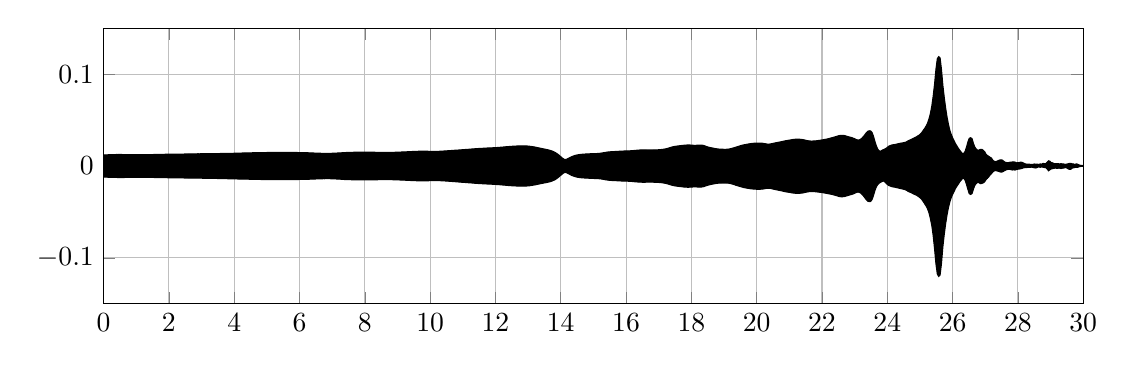
\begin{tikzpicture}

\begin{axis}[%
width=5.521in,
height=2in,
at={(0.758in,0.481in)},
xmin=0,
xmax=30,
xmajorgrids,
ymin=-0.15,
ymax=0.15,
ymajorgrids,
axis background/.style={fill=white}
]
\addplot[fill=black,draw=black,forget plot] plot table[row sep=crcr]{%
2.08333333333333e-05	0.0119891166687012\\
0.0425739952718676	0.0120701789855957\\
0.0851271572104019	0.0120600461959839\\
0.127680319148936	0.0121411085128784\\
0.17023348108747	0.0122112035751343\\
0.212786643026005	0.0122820138931274\\
0.255339804964539	0.0123153924942017\\
0.297892966903073	0.0123672485351563\\
0.340446128841608	0.0123822689056396\\
0.382999290780142	0.0124343633651733\\
0.425552452718676	0.012420654296875\\
0.46810561465721	0.0124455690383911\\
0.510658776595745	0.0124385356903076\\
0.553211938534279	0.0124293565750122\\
0.595765100472813	0.0124131441116333\\
0.638318262411347	0.0123996734619141\\
0.680871424349882	0.0123659372329712\\
0.723424586288416	0.0123772621154785\\
0.76597774822695	0.0123530626296997\\
0.808530910165485	0.0123927593231201\\
0.851084072104019	0.0123993158340454\\
0.893637234042553	0.0123468637466431\\
0.936190395981088	0.0123317241668701\\
0.978743557919622	0.0123351812362671\\
1.02129671985816	0.0123213529586792\\
1.06384988179669	0.012315034866333\\
1.10640304373522	0.0123295783996582\\
1.14895620567376	0.0123213529586792\\
1.19150936761229	0.012312650680542\\
1.23406252955083	0.0123451948165894\\
1.27661569148936	0.0123229026794434\\
1.3191688534279	0.0123435258865356\\
1.36172201536643	0.0123484134674072\\
1.40427517730496	0.0123796463012695\\
1.4468283392435	0.0123721361160278\\
1.48938150118203	0.0123879909515381\\
1.53193466312057	0.012427806854248\\
1.5744878250591	0.0124756097793579\\
1.61704098699764	0.012513279914856\\
1.65959414893617	0.0124995708465576\\
1.7021473108747	0.0125466585159302\\
1.74470047281324	0.012596607208252\\
1.78725363475177	0.0126116275787354\\
1.82980679669031	0.0126550197601318\\
1.87235995862884	0.012694239616394\\
1.91491312056738	0.0127073526382446\\
1.95746628250591	0.0127198696136475\\
2.00001944444444	0.0127586126327515\\
2.04257260638298	0.0127676725387573\\
2.08512576832151	0.012792706489563\\
2.12767893026005	0.0128316879272461\\
2.17023209219858	0.0128744840621948\\
2.21278525413712	0.0128858089447021\\
2.25533841607565	0.0128728151321411\\
2.29789157801418	0.0128904581069946\\
2.34044473995272	0.012937068939209\\
2.38299790189125	0.0129625797271729\\
2.42555106382979	0.0129508972167969\\
2.46810422576832	0.0129650831222534\\
2.51065738770686	0.0130186080932617\\
2.55321054964539	0.0130044221878052\\
2.59576371158392	0.0130490064620972\\
2.63831687352246	0.0130782127380371\\
2.68087003546099	0.0130912065505981\\
2.72342319739953	0.0131031274795532\\
2.76597635933806	0.0131406784057617\\
2.8085295212766	0.0131857395172119\\
2.85108268321513	0.0132355690002441\\
2.89363584515366	0.0132455825805664\\
2.9361890070922	0.0132309198379517\\
2.97874216903073	0.013269305229187\\
3.02129533096927	0.0133043527603149\\
3.0638484929078	0.013329029083252\\
3.10640165484634	0.0133227109909058\\
3.14895481678487	0.0133368968963623\\
3.1915079787234	0.0133442878723145\\
3.23406114066194	0.0133599042892456\\
3.27661430260047	0.0133839845657349\\
3.31916746453901	0.0133798122406006\\
3.36172062647754	0.0133849382400513\\
3.40427378841608	0.0134093761444092\\
3.44682695035461	0.013446569442749\\
3.48938011229314	0.0134661197662354\\
3.53193327423168	0.0134836435317993\\
3.57448643617021	0.013521671295166\\
3.61703959810875	0.0135370492935181\\
3.65959276004728	0.0135470628738403\\
3.70214592198582	0.0135759115219116\\
3.74469908392435	0.0136080980300903\\
3.78725224586288	0.0136371850967407\\
3.82980540780142	0.0136731863021851\\
3.87235856973995	0.0137186050415039\\
3.91491173167849	0.0137549638748169\\
3.95746489361702	0.0137441158294678\\
4.00001805555556	0.0138174295425415\\
4.04257121749409	0.013864278793335\\
4.08512437943262	0.0139147043228149\\
4.12767754137116	0.0139368772506714\\
4.17023070330969	0.0140061378479004\\
4.21278386524823	0.0140299797058105\\
4.25533702718676	0.0140790939331055\\
4.29789018912529	0.0141112804412842\\
4.34044335106383	0.0141588449478149\\
4.38299651300236	0.0141901969909668\\
4.4255496749409	0.0142172574996948\\
4.46810283687943	0.0142718553543091\\
4.51065599881797	0.0143095254898071\\
4.5532091607565	0.0143332481384277\\
4.59576232269503	0.0143661499023438\\
4.63831548463357	0.0144078731536865\\
4.6808686465721	0.0144317150115967\\
4.72342180851064	0.014464259147644\\
4.76597497044917	0.0144739151000977\\
4.80852813238771	0.0144917964935303\\
4.85108129432624	0.0145350694656372\\
4.89363445626477	0.0145490169525146\\
4.93618761820331	0.014581561088562\\
4.97874078014184	0.0145977735519409\\
5.02129394208038	0.0146069526672363\\
5.06384710401891	0.0146232843399048\\
5.10640026595745	0.0146393775939941\\
5.14895342789598	0.0146942138671875\\
5.19150658983452	0.0146994590759277\\
5.23405975177305	0.0147175788879395\\
5.27661291371158	0.0147092342376709\\
5.31916607565012	0.0147404670715332\\
5.36171923758865	0.0147354602813721\\
5.40427239952719	0.0147433280944824\\
5.44682556146572	0.0147520303726196\\
5.48937872340426	0.0147508382797241\\
5.53193188534279	0.0147504806518555\\
5.57448504728132	0.014761209487915\\
5.61703820921986	0.0147466659545898\\
5.65959137115839	0.0147426128387451\\
5.70214453309693	0.0147403478622437\\
5.74469769503546	0.0147124528884888\\
5.787250856974	0.0147058963775635\\
5.82980401891253	0.0147024393081665\\
5.87235718085106	0.0146327018737793\\
5.9149103427896	0.0146118402481079\\
5.95746350472813	0.0145947933197021\\
6.00001666666667	0.0145722627639771\\
6.0425698286052	0.0145455598831177\\
6.08512299054374	0.0144891738891602\\
6.12767615248227	0.0144437551498413\\
6.1702293144208	0.0144070386886597\\
6.21278247635934	0.014379620552063\\
6.25533563829787	0.0143579244613647\\
6.29788880023641	0.0142805576324463\\
6.34044196217494	0.0142168998718262\\
6.38299512411347	0.014191746711731\\
6.42554828605201	0.0140836238861084\\
6.46810144799054	0.0140348672866821\\
6.51065460992908	0.0139898061752319\\
6.55320777186761	0.0139384269714355\\
6.59576093380615	0.0138537883758545\\
6.63831409574468	0.0137983560562134\\
6.68086725768321	0.0137511491775513\\
6.72342041962175	0.0137094259262085\\
6.76597358156028	0.0136710405349731\\
6.80852674349882	0.0136563777923584\\
6.85107990543735	0.0136498212814331\\
6.89363306737589	0.0136363506317139\\
6.93618622931442	0.0136944055557251\\
6.97873939125296	0.0137603282928467\\
7.02129255319149	0.0138442516326904\\
7.06384571513002	0.0139046907424927\\
7.10639887706856	0.0139477252960205\\
7.14895203900709	0.014054536819458\\
7.19150520094563	0.0141353607177734\\
7.23405836288416	0.0142430067062378\\
7.27661152482269	0.0143053531646729\\
7.31916468676123	0.014385461807251\\
7.36171784869976	0.0145281553268433\\
7.4042710106383	0.0145792961120605\\
7.44682417257683	0.0146374702453613\\
7.48937733451537	0.014722466468811\\
7.5319304964539	0.0147558450698853\\
7.57448365839243	0.0148293972015381\\
7.61703682033097	0.0148519277572632\\
7.6595899822695	0.0148772001266479\\
7.70214314420804	0.0148836374282837\\
7.74469630614657	0.0149027109146118\\
7.78724946808511	0.0148898363113403\\
7.82980263002364	0.0149227380752563\\
7.87235579196217	0.0149306058883667\\
7.91490895390071	0.0149260759353638\\
7.95746211583924	0.0149365663528442\\
8.00001527777778	0.0149394273757935\\
8.04256843971631	0.0149445533752441\\
8.08512160165485	0.0149415731430054\\
8.12767476359338	0.0149654150009155\\
8.17022792553192	0.0149649381637573\\
8.21278108747045	0.014962911605835\\
8.25533424940898	0.0149157047271729\\
8.29788741134752	0.0148886442184448\\
8.34044057328605	0.0148481130599976\\
8.38299373522459	0.0147963762283325\\
8.42554689716312	0.0147671699523926\\
8.46810005910165	0.0147316455841064\\
8.51065322104019	0.0146907567977905\\
8.55320638297872	0.0146373510360718\\
8.59575954491726	0.0146878957748413\\
8.63831270685579	0.0146653652191162\\
8.68086586879433	0.0146582126617432\\
8.72341903073286	0.0146515369415283\\
8.76597219267139	0.0146892070770264\\
8.80852535460993	0.0147384405136108\\
8.85107851654846	0.0147976875305176\\
8.893631678487	0.0148004293441772\\
8.93618484042553	0.0149153470993042\\
8.97873800236407	0.0149699449539185\\
9.0212911643026	0.0150353908538818\\
9.06384432624114	0.0150772333145142\\
9.10639748817967	0.0151313543319702\\
9.1489506501182	0.0152260065078735\\
9.19150381205674	0.0153157711029053\\
9.23405697399527	0.015323281288147\\
9.27661013593381	0.0154021978378296\\
9.31916329787234	0.0154614448547363\\
9.36171645981088	0.0155340433120728\\
9.40426962174941	0.015607476234436\\
9.44682278368794	0.015711784362793\\
9.48937594562648	0.0157406330108643\\
9.53192910756501	0.0158414840698242\\
9.57448226950355	0.0159074068069458\\
9.61703543144208	0.0159391164779663\\
9.65958859338062	0.0160180330276489\\
9.70214175531915	0.0160245895385742\\
9.74469491725768	0.0160360336303711\\
9.78724807919622	0.01607346534729\\
9.82980124113475	0.0160551071166992\\
9.87235440307329	0.0160226821899414\\
9.91490756501182	0.0159975290298462\\
9.95746072695036	0.0159332752227783\\
10.0000138888889	0.0159041881561279\\
10.0425670508274	0.0158710479736328\\
10.085120212766	0.0158164501190186\\
10.1276733747045	0.0158092975616455\\
10.170226536643	0.0157977342605591\\
10.2127796985816	0.0158299207687378\\
10.2553328605201	0.0159136056900024\\
10.2978860224586	0.0159791707992554\\
10.3404391843972	0.016069769859314\\
10.3829923463357	0.0161577463150024\\
10.4255455082742	0.0162630081176758\\
10.4680986702128	0.0163758993148804\\
10.5106518321513	0.0164648294448853\\
10.5532049940898	0.0165594816207886\\
10.5957581560284	0.0166622400283813\\
10.6383113179669	0.016768217086792\\
10.6808644799054	0.0168865919113159\\
10.723417641844	0.0169931650161743\\
10.7659708037825	0.0171152353286743\\
10.808523965721	0.0171926021575928\\
10.8510771276596	0.017282247543335\\
10.8936302895981	0.0174212455749512\\
10.9361834515366	0.0175200700759888\\
10.9787366134752	0.0176385641098022\\
11.0212897754137	0.0177961587905884\\
11.0638429373522	0.0178617238998413\\
11.1063960992908	0.0179822444915771\\
11.1489492612293	0.0180516242980957\\
11.1915024231678	0.0181763172149658\\
11.2340555851064	0.0183032751083374\\
11.2766087470449	0.0184470415115356\\
11.3191619089835	0.0185744762420654\\
11.361715070922	0.0186715126037598\\
11.4042682328605	0.0187947750091553\\
11.4468213947991	0.0189191102981567\\
11.4893745567376	0.0189660787582397\\
11.5319277186761	0.0190688371658325\\
11.5744808806147	0.019160270690918\\
11.6170340425532	0.0192372798919678\\
11.6595872044917	0.0193090438842773\\
11.7021403664303	0.019400954246521\\
11.7446935283688	0.0195177793502808\\
11.7872466903073	0.0195590257644653\\
11.8297998522459	0.0196257829666138\\
11.8723530141844	0.0197001695632935\\
11.9149061761229	0.0197663307189941\\
11.9574593380615	0.0198649168014526\\
12.0000125	0.0199562311172485\\
12.0425656619385	0.0200393199920654\\
12.0851188238771	0.0201531648635864\\
12.1276719858156	0.0202683210372925\\
12.1702251477541	0.0203834772109985\\
12.2127783096927	0.0205181837081909\\
12.2553314716312	0.0206431150436401\\
12.2978846335697	0.020803689956665\\
12.3404377955083	0.0209430456161499\\
12.3829909574468	0.0210655927658081\\
12.4255441193853	0.0211613178253174\\
12.4680972813239	0.0213009119033813\\
12.5106504432624	0.0214111804962158\\
12.5532036052009	0.0215167999267578\\
12.5957567671395	0.0215667486190796\\
12.638309929078	0.0216765403747559\\
12.6808630910165	0.0217441320419312\\
12.7234162529551	0.0217874050140381\\
12.7659694148936	0.0218304395675659\\
12.8085225768322	0.0218579769134521\\
12.8510757387707	0.0218334197998047\\
12.8936289007092	0.0218534469604492\\
12.9361820626478	0.0217874050140381\\
12.9787352245863	0.0216927528381348\\
13.0212883865248	0.021544337272644\\
13.0638415484634	0.021371603012085\\
13.1063947104019	0.0211578607559204\\
13.1489478723404	0.0209262371063232\\
13.191501034279	0.0206685066223145\\
13.2340541962175	0.0203869342803955\\
13.276607358156	0.0200080871582031\\
13.3191605200946	0.019722580909729\\
13.3617136820331	0.0194058418273926\\
13.4042668439716	0.0190954208374023\\
13.4468200059102	0.0187587738037109\\
13.4893731678487	0.0184516906738281\\
13.5319263297872	0.0181584358215332\\
13.5744794917258	0.0178221464157104\\
13.6170326536643	0.0174729824066162\\
13.6595858156028	0.0171077251434326\\
13.7021389775414	0.016639232635498\\
13.7446921394799	0.0161151885986328\\
13.7872453014184	0.0154547691345215\\
13.829798463357	0.0146360397338867\\
13.8723516252955	0.0137324333190918\\
13.914904787234	0.0126259326934814\\
13.9574579491726	0.0113997459411621\\
14.0000111111111	0.0100481510162354\\
14.0425642730496	0.00874054431915283\\
14.0851174349882	0.00763881206512451\\
14.1276705969267	0.00698995590209961\\
14.1702237588652	0.00721240043640137\\
14.2127769208038	0.0078728199005127\\
14.2553300827423	0.00864839553833008\\
14.2978832446809	0.00943124294281006\\
14.3404364066194	0.010124683380127\\
14.3829895685579	0.0107450485229492\\
14.4255427304965	0.0112762451171875\\
14.468095892435	0.0117151737213135\\
14.5106490543735	0.0120129585266113\\
14.5532022163121	0.0122971534729004\\
14.5957553782506	0.0124787092208862\\
14.6383085401891	0.0126643180847168\\
14.6808617021277	0.0127860307693481\\
14.7234148640662	0.0129104852676392\\
14.7659680260047	0.013019323348999\\
14.8085211879433	0.0130923986434937\\
14.8510743498818	0.0131598711013794\\
14.8936275118203	0.0132442712783813\\
14.9361806737589	0.0132671594619751\\
14.9787338356974	0.0133401155471802\\
15.0212869976359	0.0133960247039795\\
15.0638401595745	0.0134508609771729\\
15.106393321513	0.0134987831115723\\
15.1489464834515	0.0135847330093384\\
15.1914996453901	0.0137389898300171\\
15.2340528073286	0.0139615535736084\\
15.2766059692671	0.0141968727111816\\
15.3191591312057	0.0144667625427246\\
15.3617122931442	0.0147184133529663\\
15.4042654550827	0.0149639844894409\\
15.4468186170213	0.0151892900466919\\
15.4893717789598	0.0153195858001709\\
15.5319249408983	0.0154467821121216\\
15.5744781028369	0.0155524015426636\\
15.6170312647754	0.0156270265579224\\
15.6595844267139	0.0157109498977661\\
15.7021375886525	0.0157914161682129\\
15.744690750591	0.0158919095993042\\
15.7872439125296	0.0159846544265747\\
15.8297970744681	0.0160763263702393\\
15.8723502364066	0.0161715745925903\\
15.9149033983452	0.0162194967269897\\
15.9574565602837	0.0162959098815918\\
16.0000097222222	0.0163196325302124\\
16.0425628841608	0.0163333415985107\\
16.0851160460993	0.0164139270782471\\
16.1276692080378	0.0164852142333984\\
16.1702223699764	0.016596794128418\\
16.2127755319149	0.0167173147201538\\
16.2553286938534	0.016867995262146\\
16.297881855792	0.0169942378997803\\
16.3404350177305	0.0171358585357666\\
16.382988179669	0.017247200012207\\
16.4255413416076	0.0173672437667847\\
16.4680945035461	0.0174224376678467\\
16.5106476654846	0.0174494981765747\\
16.5532008274232	0.0174441337585449\\
16.5957539893617	0.0174261331558228\\
16.6383071513002	0.0173689126968384\\
16.6808603132388	0.017351508140564\\
16.7234134751773	0.0173255205154419\\
16.7659666371158	0.0173234939575195\\
16.8085197990544	0.0173735618591309\\
16.8510729609929	0.0174065828323364\\
16.8936261229314	0.0174649953842163\\
16.93617928487	0.017520546913147\\
16.9787324468085	0.0175772905349731\\
17.021285608747	0.017709493637085\\
17.0638387706856	0.017842173576355\\
17.1063919326241	0.0179907083511353\\
17.1489450945626	0.0182030200958252\\
17.1914982565012	0.0184568166732788\\
17.2340514184397	0.0187783241271973\\
17.2766045803783	0.0191693305969238\\
17.3191577423168	0.0196816921234131\\
17.3617109042553	0.0201215744018555\\
17.4042640661939	0.0205991268157959\\
17.4468172281324	0.0209838151931763\\
17.4893703900709	0.0212384462356567\\
17.5319235520095	0.0214720964431763\\
17.574476713948	0.0217106342315674\\
17.6170298758865	0.0218876600265503\\
17.6595830378251	0.0220842361450195\\
17.7021361997636	0.0222510099411011\\
17.7446893617021	0.0224254131317139\\
17.7872425236407	0.0225731134414673\\
17.8297956855792	0.0227036476135254\\
17.8723488475177	0.0228030681610107\\
17.9149020094563	0.0228255987167358\\
17.9574551713948	0.0227867364883423\\
18.0000083333333	0.0226969718933105\\
18.0425614952719	0.0225468873977661\\
18.0851146572104	0.022442102432251\\
18.1276678191489	0.0224337577819824\\
18.1702209810875	0.0225523710250854\\
18.212774143026	0.0226941108703613\\
18.2553273049645	0.0227112770080566\\
18.2978804669031	0.0226702690124512\\
18.3404336288416	0.0225247144699097\\
18.3829867907801	0.022191047668457\\
18.4255399527187	0.0216506719589233\\
18.4680931146572	0.0210781097412109\\
18.5106462765957	0.0205855369567871\\
18.5531994385343	0.0202169418334961\\
18.5957526004728	0.0198911428451538\\
18.6383057624113	0.0195983648300171\\
18.6808589243499	0.0192761421203613\\
18.7234120862884	0.0189481973648071\\
18.765965248227	0.0187180042266846\\
18.8085184101655	0.0185004472732544\\
18.851071572104	0.0183453559875488\\
18.8936247340426	0.0182894468307495\\
18.9361778959811	0.018202543258667\\
18.9787310579196	0.0181392431259155\\
19.0212842198582	0.018133282661438\\
19.0638373817967	0.0181257724761963\\
19.1063905437352	0.0182130336761475\\
19.1489437056738	0.0184046030044556\\
19.1914968676123	0.0186821222305298\\
19.2340500295508	0.0190776586532593\\
19.2766031914894	0.0195093154907227\\
19.3191563534279	0.0199741125106812\\
19.3617095153664	0.020482063293457\\
19.404262677305	0.0209068059921265\\
19.4468158392435	0.0214110612869263\\
19.489369001182	0.0218472480773926\\
19.5319221631206	0.0223336219787598\\
19.5744753250591	0.0227125883102417\\
19.6170284869976	0.0230491161346436\\
19.6595816489362	0.0233137607574463\\
19.7021348108747	0.0236597061157227\\
19.7446879728132	0.0238858461380005\\
19.7872411347518	0.0241514444351196\\
19.8297942966903	0.0243535041809082\\
19.8723474586288	0.0245242118835449\\
19.9149006205674	0.0246922969818115\\
19.9574537825059	0.0247610807418823\\
20.0000069444444	0.0248315334320068\\
20.042560106383	0.0248575210571289\\
20.0851132683215	0.0248454809188843\\
20.12766643026	0.0248016119003296\\
20.1702195921986	0.0247161388397217\\
20.2127727541371	0.0244866609573364\\
20.2553259160756	0.0242441892623901\\
20.2978790780142	0.0239566564559937\\
20.3404322399527	0.0237118005752563\\
20.3829854018913	0.0237652063369751\\
20.4255385638298	0.0240160226821899\\
20.4680917257683	0.0243251323699951\\
20.5106448877069	0.0246405601501465\\
20.5531980496454	0.0249805450439453\\
20.5957512115839	0.0253318548202515\\
20.6383043735225	0.025571346282959\\
20.680857535461	0.0258880853652954\\
20.7234106973995	0.0261416435241699\\
20.7659638593381	0.0264977216720581\\
20.8085170212766	0.0268567800521851\\
20.8510701832151	0.0271531343460083\\
20.8936233451537	0.0274865627288818\\
20.9361765070922	0.027751088142395\\
20.9787296690307	0.0279955863952637\\
21.0212828309693	0.0282137393951416\\
21.0638359929078	0.0284777879714966\\
21.1063891548463	0.0287666320800781\\
21.1489423167849	0.0289372205734253\\
21.1914954787234	0.0290979146957397\\
21.2340486406619	0.0291520357131958\\
21.2766018026005	0.0291374921798706\\
21.319154964539	0.0290536880493164\\
21.3617081264775	0.0289229154586792\\
21.4042612884161	0.0287134647369385\\
21.4468144503546	0.0284314155578613\\
21.4893676122931	0.0280815362930298\\
21.5319207742317	0.0277200937271118\\
21.5744739361702	0.027424693107605\\
21.6170270981087	0.0271998643875122\\
21.6595802600473	0.0271004438400269\\
21.7021334219858	0.0271096229553223\\
21.7446865839243	0.027174711227417\\
21.7872397458629	0.0272704362869263\\
21.8297929078014	0.0274029970169067\\
21.87234606974	0.0276217460632324\\
21.9148992316785	0.0278003215789795\\
21.957452393617	0.0280568599700928\\
22.0000055555556	0.028328537940979\\
22.0425587174941	0.0285825729370117\\
22.0851118794326	0.0288678407669067\\
22.1276650413712	0.0291299819946289\\
22.1702182033097	0.029487133026123\\
22.2127713652482	0.029843807220459\\
22.2553245271868	0.0302610397338867\\
22.2978776891253	0.0306540727615356\\
22.3404308510638	0.0310933589935303\\
22.3829840130024	0.0315306186676025\\
22.4255371749409	0.0319411754608154\\
22.4680903368794	0.0324456691741943\\
22.510643498818	0.0329251289367676\\
22.5531966607565	0.0331741571426392\\
22.595749822695	0.0333001613616943\\
22.6383029846336	0.0332827568054199\\
22.6808561465721	0.0331307649612427\\
22.7234093085106	0.0327298641204834\\
22.7659624704492	0.032257080078125\\
22.8085156323877	0.0318152904510498\\
22.8510687943262	0.0313825607299805\\
22.8936219562648	0.0310475826263428\\
22.9361751182033	0.0305105447769165\\
22.9787282801418	0.0299614667892456\\
23.0212814420804	0.0292130708694458\\
23.0638346040189	0.0285649299621582\\
23.1063877659574	0.0281169414520264\\
23.148940927896	0.0285003185272217\\
23.1914940898345	0.0293340682983398\\
23.234047251773	0.0306720733642578\\
23.2766004137116	0.0323584079742432\\
23.3191535756501	0.0342948436737061\\
23.3617067375887	0.0363030433654785\\
23.4042598995272	0.0377959012985229\\
23.4468130614657	0.0382936000823975\\
23.4893662234043	0.0381671190261841\\
23.5319193853428	0.0364677906036377\\
23.5744725472813	0.0325307846069336\\
23.6170257092199	0.0271339416503906\\
23.6595788711584	0.0222088098526001\\
23.7021320330969	0.0186933279037476\\
23.7446851950355	0.0165317058563232\\
23.787238356974	0.0160146951675415\\
23.8297915189125	0.0168312788009644\\
23.8723446808511	0.0176469087600708\\
23.9148978427896	0.018263578414917\\
23.9574510047281	0.018985390663147\\
24.0000041666667	0.0202053785324097\\
24.0425573286052	0.0214619636535645\\
24.0851104905437	0.022052526473999\\
24.1276636524823	0.0227371454238892\\
24.1702168144208	0.0230492353439331\\
24.2127699763593	0.0232532024383545\\
24.2553231382979	0.0234876871109009\\
24.2978763002364	0.0238732099533081\\
24.3404294621749	0.0242279767990112\\
24.3829826241135	0.0246217250823975\\
24.425535786052	0.0249172449111938\\
24.4680889479905	0.0250427722930908\\
24.5106421099291	0.0254533290863037\\
24.5531952718676	0.0256302356719971\\
24.5957484338061	0.0264087915420532\\
24.6383015957447	0.0274142026901245\\
24.6808547576832	0.028038501739502\\
24.7234079196217	0.0287498235702515\\
24.7659610815603	0.029454231262207\\
24.8085142434988	0.0302711725234985\\
24.8510674054374	0.0310555696487427\\
24.8936205673759	0.0316926240921021\\
24.9361737293144	0.0327839851379395\\
24.978726891253	0.033631443977356\\
25.0212800531915	0.0349727869033813\\
25.06383321513	0.0368019342422485\\
25.1063863770686	0.0389444828033447\\
25.1489395390071	0.041167140007019\\
25.1914927009456	0.0434926748275757\\
25.2340458628842	0.0467634201049805\\
25.2765990248227	0.0511188507080078\\
25.3191521867612	0.057016134262085\\
25.3617053486998	0.0649584531784058\\
25.4042585106383	0.0758386850357056\\
25.4468116725768	0.0889134407043457\\
25.4893648345154	0.105216860771179\\
25.5319179964539	0.116796731948853\\
25.5744711583924	0.119030594825745\\
25.617024320331	0.11763870716095\\
25.6595774822695	0.104707360267639\\
25.702130644208	0.0874937772750854\\
25.7446838061466	0.0744110345840454\\
25.7872369680851	0.06288743019104\\
25.8297901300236	0.0530766248703003\\
25.8723432919622	0.0452847480773926\\
25.9148964539007	0.0387722253799438\\
25.9574496158392	0.0343474149703979\\
26.0000027777778	0.030636191368103\\
26.0425559397163	0.0276141166687012\\
26.0851091016548	0.0244072675704956\\
26.1276622635934	0.0219786167144775\\
26.1702154255319	0.0195002555847168\\
26.2127685874705	0.017353892326355\\
26.255321749409	0.0152941942214966\\
26.2978749113475	0.0136313438415527\\
26.3404280732861	0.0135471820831299\\
26.3829812352246	0.0158743858337402\\
26.4255343971631	0.0204313993453979\\
26.4680875591017	0.0261033773422241\\
26.5106407210402	0.0301426649093628\\
26.5531938829787	0.0307470560073853\\
26.5957470449173	0.0297296047210693\\
26.6383002068558	0.0243973731994629\\
26.6808533687943	0.0204536914825439\\
26.7234065307329	0.0183995962142944\\
26.7659596926714	0.0170893669128418\\
26.8085128546099	0.0173263549804688\\
26.8510660165485	0.01812744140625\\
26.893619178487	0.0181320905685425\\
26.9361723404255	0.0170766115188599\\
26.9787255023641	0.0156316757202148\\
27.0212786643026	0.0127568244934082\\
27.0638318262411	0.0114500522613525\\
27.1063849881797	0.0104755163192749\\
27.1489381501182	0.00944781303405762\\
27.1914913120567	0.00852572917938232\\
27.2340444739953	0.00608611106872559\\
27.2765976359338	0.00501561164855957\\
27.3191507978723	0.00464582443237305\\
27.3617039598109	0.0052187442779541\\
27.4042571217494	0.00589883327484131\\
27.4468102836879	0.00653588771820068\\
27.4893634456265	0.00666952133178711\\
27.531916607565	0.00618875026702881\\
27.5744697695035	0.00481438636779785\\
27.6170229314421	0.00392997264862061\\
27.6595760933806	0.00364542007446289\\
27.7021292553192	0.00357687473297119\\
27.7446824172577	0.0039665699005127\\
27.7872355791962	0.00409770011901855\\
27.8297887411348	0.00434184074401855\\
27.8723419030733	0.00437593460083008\\
27.9148950650118	0.00416827201843262\\
27.9574482269504	0.00337409973144531\\
28.0000013888889	0.00351810455322266\\
28.0425545508274	0.00388240814208984\\
28.085107712766	0.00404250621795654\\
28.1276608747045	0.00395500659942627\\
28.170214036643	0.0031973123550415\\
28.2127671985816	0.00237417221069336\\
28.2553203605201	0.00200951099395752\\
28.2978735224586	0.00202393531799316\\
28.3404266843972	0.00191807746887207\\
28.3829798463357	0.00173366069793701\\
28.4255330082742	0.00155413150787354\\
28.4680861702128	0.00181210041046143\\
28.5106393321513	0.00211071968078613\\
28.5531924940898	0.00176608562469482\\
28.5957456560284	0.00202560424804688\\
28.6382988179669	0.00156760215759277\\
28.6808519799054	0.00219047069549561\\
28.723405141844	0.00191926956176758\\
28.7659583037825	0.00270414352416992\\
28.808511465721	0.00257468223571777\\
28.8510646276596	0.00250673294067383\\
28.8936177895981	0.00388991832733154\\
28.9361709515366	0.00561344623565674\\
28.9787241134752	0.00521004199981689\\
29.0212772754137	0.00365424156188965\\
29.0638304373522	0.0033804178237915\\
29.1063835992908	0.00262355804443359\\
29.1489367612293	0.00234818458557129\\
29.1914899231679	0.0025477409362793\\
29.2340430851064	0.00256478786468506\\
29.2765962470449	0.00208735466003418\\
29.3191494089835	0.00250005722045898\\
29.361702570922	0.00219547748565674\\
29.4042557328605	0.00211131572723389\\
29.4468088947991	0.00169658660888672\\
29.4893620567376	0.00201320648193359\\
29.5319152186761	0.00230777263641357\\
29.5744683806147	0.00270867347717285\\
29.6170215425532	0.0027766227722168\\
29.6595747044917	0.00231611728668213\\
29.7021278664303	0.00214874744415283\\
29.7446810283688	0.00160884857177734\\
29.7872341903073	0.00224554538726807\\
29.8297873522459	0.00190925598144531\\
29.8723405141844	0.00109612941741943\\
29.9148936761229	0.000704288482666016\\
29.9574468380615	0.00048518180847168\\
30	0.000414729118347168\\
}
\closedcycle;
\addplot[fill=black,draw=black,forget plot] plot table[row sep=crcr]{%
2.08333333333333e-05	-0.012113094329834\\
0.0425739952718676	-0.0121138095855713\\
0.0851271572104019	-0.0121619701385498\\
0.127680319148936	-0.0122429132461548\\
0.17023348108747	-0.0122907161712646\\
0.212786643026005	-0.0123883485794067\\
0.255339804964539	-0.0124168395996094\\
0.297892966903073	-0.0124434232711792\\
0.340446128841608	-0.01246178150177\\
0.382999290780142	-0.0125032663345337\\
0.425552452718676	-0.0125099420547485\\
0.46810561465721	-0.0125166177749634\\
0.510658776595745	-0.0125166177749634\\
0.553211938534279	-0.0125176906585693\\
0.595765100472813	-0.0125076770782471\\
0.638318262411347	-0.0125123262405396\\
0.680871424349882	-0.0124843120574951\\
0.723424586288416	-0.0124874114990234\\
0.76597774822695	-0.0124468803405762\\
0.808530910165485	-0.0124509334564209\\
0.851084072104019	-0.0124367475509644\\
0.893637234042553	-0.0124189853668213\\
0.936190395981088	-0.012392520904541\\
0.978743557919622	-0.0124033689498901\\
1.02129671985816	-0.0123730897903442\\
1.06384988179669	-0.0124198198318481\\
1.10640304373522	-0.0123876333236694\\
1.14895620567376	-0.0124117136001587\\
1.19150936761229	-0.0123980045318604\\
1.23406252955083	-0.0124258995056152\\
1.27661569148936	-0.012415885925293\\
1.3191688534279	-0.0124626159667969\\
1.36172201536643	-0.012446403503418\\
1.40427517730496	-0.0124740600585938\\
1.4468283392435	-0.0124877691268921\\
1.48938150118203	-0.0125036239624023\\
1.53193466312057	-0.0125057697296143\\
1.5744878250591	-0.0125240087509155\\
1.61704098699764	-0.0125665664672852\\
1.65959414893617	-0.012586236000061\\
1.7021473108747	-0.0126203298568726\\
1.74470047281324	-0.0126328468322754\\
1.78725363475177	-0.0126634836196899\\
1.82980679669031	-0.0127276182174683\\
1.87235995862884	-0.0127447843551636\\
1.91491312056738	-0.0127626657485962\\
1.95746628250591	-0.0127805471420288\\
2.00001944444444	-0.0128178596496582\\
2.04257260638298	-0.0128737688064575\\
2.08512576832151	-0.0128716230392456\\
2.12767893026005	-0.0129257440567017\\
2.17023209219858	-0.0129240751266479\\
2.21278525413712	-0.0129307508468628\\
2.25533841607565	-0.0129609107971191\\
2.29789157801418	-0.0129433870315552\\
2.34044473995272	-0.0129650831222534\\
2.38299790189125	-0.012988805770874\\
2.42555106382979	-0.013023853302002\\
2.46810422576832	-0.0130585432052612\\
2.51065738770686	-0.0130890607833862\\
2.55321054964539	-0.0130822658538818\\
2.59576371158392	-0.0131436586380005\\
2.63831687352246	-0.0131477117538452\\
2.68087003546099	-0.0131758451461792\\
2.72342319739953	-0.0131961107254028\\
2.76597635933806	-0.0131841897964478\\
2.8085295212766	-0.0132342576980591\\
2.85108268321513	-0.0132158994674683\\
2.89363584515366	-0.0132571458816528\\
2.9361890070922	-0.0132758617401123\\
2.97874216903073	-0.0133143663406372\\
3.02129533096927	-0.0133262872695923\\
3.0638484929078	-0.0133285522460938\\
3.10640165484634	-0.0133302211761475\\
3.14895481678487	-0.0133769512176514\\
3.1915079787234	-0.0133914947509766\\
3.23406114066194	-0.013434886932373\\
3.27661430260047	-0.0134336948394775\\
3.31916746453901	-0.0134991407394409\\
3.36172062647754	-0.0134928226470947\\
3.40427378841608	-0.0135328769683838\\
3.44682695035461	-0.0135462284088135\\
3.48938011229314	-0.0136126279830933\\
3.53193327423168	-0.0136435031890869\\
3.57448643617021	-0.0136560201644897\\
3.61703959810875	-0.0137197971343994\\
3.65959276004728	-0.0137335062026978\\
3.70214592198582	-0.0137761831283569\\
3.74469908392435	-0.013823390007019\\
3.78725224586288	-0.0138667821884155\\
3.82980540780142	-0.0138909816741943\\
3.87235856973995	-0.0139669179916382\\
3.91491173167849	-0.013978123664856\\
3.95746489361702	-0.0140331983566284\\
4.00001805555556	-0.0140602588653564\\
4.04257121749409	-0.0141162872314453\\
4.08512437943262	-0.0141328573226929\\
4.12767754137116	-0.0141587257385254\\
4.17023070330969	-0.0142300128936768\\
4.21278386524823	-0.0142171382904053\\
4.25533702718676	-0.0142806768417358\\
4.29789018912529	-0.0142964124679565\\
4.34044335106383	-0.0143094062805176\\
4.38299651300236	-0.014351487159729\\
4.4255496749409	-0.0144045352935791\\
4.46810283687943	-0.0144202709197998\\
4.51065599881797	-0.0144541263580322\\
4.5532091607565	-0.0145096778869629\\
4.59576232269503	-0.0145117044448853\\
4.63831548463357	-0.0145535469055176\\
4.6808686465721	-0.0145788192749023\\
4.72342180851064	-0.0146294832229614\\
4.76597497044917	-0.0146406888961792\\
4.80852813238771	-0.0146827697753906\\
4.85108129432624	-0.0147362947463989\\
4.89363445626477	-0.0147140026092529\\
4.93618761820331	-0.014751672744751\\
4.97874078014184	-0.0147874355316162\\
5.02129394208038	-0.0148072242736816\\
5.06384710401891	-0.0147817134857178\\
5.10640026595745	-0.0148316621780396\\
5.14895342789598	-0.0148299932479858\\
5.19150658983452	-0.0148706436157227\\
5.23405975177305	-0.0148839950561523\\
5.27661291371158	-0.0149160623550415\\
5.31916607565012	-0.0149294137954712\\
5.36171923758865	-0.0149381160736084\\
5.40427239952719	-0.0149247646331787\\
5.44682556146572	-0.0149132013320923\\
5.48937872340426	-0.0149377584457397\\
5.53193188534279	-0.014884352684021\\
5.57448504728132	-0.0148860216140747\\
5.61703820921986	-0.0148693323135376\\
5.65959137115839	-0.0148825645446777\\
5.70214453309693	-0.0148489475250244\\
5.74469769503546	-0.0148134231567383\\
5.787250856974	-0.0148054361343384\\
5.82980401891253	-0.0147805213928223\\
5.87235718085106	-0.0147774219512939\\
5.9149103427896	-0.014757513999939\\
5.95746350472813	-0.014722466468811\\
6.00001666666667	-0.0146836042404175\\
6.0425698286052	-0.0146520137786865\\
6.08512299054374	-0.0146064758300781\\
6.12767615248227	-0.0145918130874634\\
6.1702293144208	-0.0145655870437622\\
6.21278247635934	-0.0145376920700073\\
6.25533563829787	-0.0144726037979126\\
6.29788880023641	-0.0144317150115967\\
6.34044196217494	-0.0143640041351318\\
6.38299512411347	-0.0143401622772217\\
6.42554828605201	-0.0142568349838257\\
6.46810144799054	-0.0141904354095459\\
6.51065460992908	-0.014129638671875\\
6.55320777186761	-0.0140664577484131\\
6.59576093380615	-0.0139951705932617\\
6.63831409574468	-0.0139943361282349\\
6.68086725768321	-0.013921856880188\\
6.72342041962175	-0.0138674974441528\\
6.76597358156028	-0.0138700008392334\\
6.80852674349882	-0.0138266086578369\\
6.85107990543735	-0.0138033628463745\\
6.89363306737589	-0.0138267278671265\\
6.93618622931442	-0.0138603448867798\\
6.97873939125296	-0.0139093399047852\\
7.02129255319149	-0.0139569044113159\\
7.06384571513002	-0.0140078067779541\\
7.10639887706856	-0.0141046047210693\\
7.14895203900709	-0.0142216682434082\\
7.19150520094563	-0.0143018960952759\\
7.23405836288416	-0.014325737953186\\
7.27661152482269	-0.0144776105880737\\
7.31916468676123	-0.014553427696228\\
7.36171784869976	-0.0146636962890625\\
7.4042710106383	-0.0147805213928223\\
7.44682417257683	-0.0147774219512939\\
7.48937733451537	-0.0148789882659912\\
7.5319304964539	-0.014926552772522\\
7.57448365839243	-0.0149526596069336\\
7.61703682033097	-0.0149977207183838\\
7.6595899822695	-0.0150274038314819\\
7.70214314420804	-0.0150216817855835\\
7.74469630614657	-0.0150569677352905\\
7.78724946808511	-0.0150774717330933\\
7.82980263002364	-0.0150794982910156\\
7.87235579196217	-0.0150913000106812\\
7.91490895390071	-0.0150800943374634\\
7.95746211583924	-0.0151046514511108\\
8.00001527777778	-0.0151209831237793\\
8.04256843971631	-0.0151158571243286\\
8.08512160165485	-0.0151230096817017\\
8.12767476359338	-0.0151163339614868\\
8.17022792553192	-0.0151170492172241\\
8.21278108747045	-0.015113353729248\\
8.25533424940898	-0.0150854587554932\\
8.29788741134752	-0.0150784254074097\\
8.34044057328605	-0.014992356300354\\
8.38299373522459	-0.0149698257446289\\
8.42554689716312	-0.0149426460266113\\
8.46810005910165	-0.014917254447937\\
8.51065322104019	-0.0148546695709229\\
8.55320638297872	-0.014845609664917\\
8.59575954491726	-0.0148199796676636\\
8.63831270685579	-0.014836311340332\\
8.68086586879433	-0.0148338079452515\\
8.72341903073286	-0.01482093334198\\
8.76597219267139	-0.0148725509643555\\
8.80852535460993	-0.0149130821228027\\
8.85107851654846	-0.0149532556533813\\
8.893631678487	-0.0150277614593506\\
8.93618484042553	-0.0150550603866577\\
8.97873800236407	-0.0151125192642212\\
9.0212911643026	-0.0151705741882324\\
9.06384432624114	-0.0152268409729004\\
9.10639748817967	-0.0152989625930786\\
9.1489506501182	-0.0153621435165405\\
9.19150381205674	-0.0154212713241577\\
9.23405697399527	-0.0154908895492554\\
9.27661013593381	-0.0155407190322876\\
9.31916329787234	-0.0156335830688477\\
9.36171645981088	-0.0156954526901245\\
9.40426962174941	-0.0157989263534546\\
9.44682278368794	-0.0158728361129761\\
9.48937594562648	-0.0159257650375366\\
9.53192910756501	-0.0159800052642822\\
9.57448226950355	-0.0160501003265381\\
9.61703543144208	-0.0160759687423706\\
9.65958859338062	-0.0161364078521729\\
9.70214175531915	-0.0161623954772949\\
9.74469491725768	-0.0161715745925903\\
9.78724807919622	-0.0161818265914917\\
9.82980124113475	-0.0161776542663574\\
9.87235440307329	-0.0161452293395996\\
9.91490756501182	-0.0161435604095459\\
9.95746072695036	-0.0160480737686157\\
10.0000138888889	-0.0160074234008789\\
10.0425670508274	-0.0159573554992676\\
10.085120212766	-0.0158952474594116\\
10.1276733747045	-0.0158969163894653\\
10.170226536643	-0.0158489942550659\\
10.2127796985816	-0.0158857107162476\\
10.2553328605201	-0.0159428119659424\\
10.2978860224586	-0.0159850120544434\\
10.3404391843972	-0.0160963535308838\\
10.3829923463357	-0.0161405801773071\\
10.4255455082742	-0.0162266492843628\\
10.4680986702128	-0.0163537263870239\\
10.5106518321513	-0.016463041305542\\
10.5532049940898	-0.0165412425994873\\
10.5957581560284	-0.0166654586791992\\
10.6383113179669	-0.0167874097824097\\
10.6808644799054	-0.0168699026107788\\
10.723417641844	-0.0170114040374756\\
10.7659708037825	-0.0171157121658325\\
10.808523965721	-0.0172432661056519\\
10.8510771276596	-0.0173588991165161\\
10.8936302895981	-0.0174890756607056\\
10.9361834515366	-0.0176196098327637\\
10.9787366134752	-0.0177257061004639\\
11.0212897754137	-0.0178505182266235\\
11.0638429373522	-0.0179296731948853\\
11.1063960992908	-0.0180578231811523\\
11.1489492612293	-0.0181858539581299\\
11.1915024231678	-0.0183118581771851\\
11.2340555851064	-0.0184283256530762\\
11.2766087470449	-0.0185163021087646\\
11.3191619089835	-0.0186553001403809\\
11.361715070922	-0.018781304359436\\
11.4042682328605	-0.0188863277435303\\
11.4468213947991	-0.0190004110336304\\
11.4893745567376	-0.0191012620925903\\
11.5319277186761	-0.0192080736160278\\
11.5744808806147	-0.0192803144454956\\
11.6170340425532	-0.0193767547607422\\
11.6595872044917	-0.019465446472168\\
11.7021403664303	-0.0195423364639282\\
11.7446935283688	-0.0196044445037842\\
11.7872466903073	-0.0196491479873657\\
11.8297998522459	-0.0197625160217285\\
11.8723530141844	-0.019813060760498\\
11.9149061761229	-0.0199345350265503\\
11.9574593380615	-0.0199878215789795\\
12.0000125	-0.0200809240341187\\
12.0425656619385	-0.020203709602356\\
12.0851188238771	-0.0202950239181519\\
12.1276719858156	-0.0203992128372192\\
12.1702251477541	-0.0205478668212891\\
12.2127783096927	-0.0206730365753174\\
12.2553314716312	-0.0208123922348022\\
12.2978846335697	-0.0209157466888428\\
12.3404377955083	-0.0210793018341064\\
12.3829909574468	-0.0212075710296631\\
12.4255441193853	-0.0213204622268677\\
12.4680972813239	-0.0214297771453857\\
12.5106504432624	-0.0215437412261963\\
12.5532036052009	-0.0216523408889771\\
12.5957567671395	-0.0217057466506958\\
12.638309929078	-0.0217827558517456\\
12.6808630910165	-0.0218445062637329\\
12.7234162529551	-0.0219008922576904\\
12.7659694148936	-0.0219255685806274\\
12.8085225768322	-0.0219546556472778\\
12.8510757387707	-0.0219559669494629\\
12.8936289007092	-0.0219188928604126\\
12.9361820626478	-0.0218608379364014\\
12.9787352245863	-0.0217357873916626\\
13.0212883865248	-0.0215924978256226\\
13.0638415484634	-0.0214599370956421\\
13.1063947104019	-0.0211890935897827\\
13.1489478723404	-0.0209450721740723\\
13.191501034279	-0.0206962823867798\\
13.2340541962175	-0.0204030275344849\\
13.276607358156	-0.0200580358505249\\
13.3191605200946	-0.0197618007659912\\
13.3617136820331	-0.0194422006607056\\
13.4042668439716	-0.0191107988357544\\
13.4468200059102	-0.0188400745391846\\
13.4893731678487	-0.0184996128082275\\
13.5319263297872	-0.0182305574417114\\
13.5744794917258	-0.0179266929626465\\
13.6170326536643	-0.017613410949707\\
13.6595858156028	-0.0172340869903564\\
13.7021389775414	-0.0167717933654785\\
13.7446921394799	-0.0162343978881836\\
13.7872453014184	-0.0155785083770752\\
13.829798463357	-0.0147982835769653\\
13.8723516252955	-0.0138078927993774\\
13.914904787234	-0.0126904249191284\\
13.9574579491726	-0.0114437341690063\\
14.0000111111111	-0.0101087093353271\\
14.0425642730496	-0.00886237621307373\\
14.0851174349882	-0.00769996643066406\\
14.1276705969267	-0.00697076320648193\\
14.1702237588652	-0.00723934173583984\\
14.2127769208038	-0.0079423189163208\\
14.2553300827423	-0.00873672962188721\\
14.2978832446809	-0.00956249237060547\\
14.3404364066194	-0.010346531867981\\
14.3829895685579	-0.0109330415725708\\
14.4255427304965	-0.0114353895187378\\
14.468095892435	-0.0118498802185059\\
14.5106490543735	-0.0122239589691162\\
14.5532022163121	-0.0124701261520386\\
14.5957553782506	-0.0126818418502808\\
14.6383085401891	-0.0128611326217651\\
14.6808617021277	-0.0129830837249756\\
14.7234148640662	-0.013073205947876\\
14.7659680260047	-0.0131728649139404\\
14.8085211879433	-0.0132454633712769\\
14.8510743498818	-0.0133155584335327\\
14.8936275118203	-0.0134053230285645\\
14.9361806737589	-0.0134707689285278\\
14.9787338356974	-0.013554573059082\\
15.0212869976359	-0.0136101245880127\\
15.0638401595745	-0.0136501789093018\\
15.106393321513	-0.0137456655502319\\
15.1489464834515	-0.0138136148452759\\
15.1914996453901	-0.0139260292053223\\
15.2340528073286	-0.0141358375549316\\
15.2766059692671	-0.0143586397171021\\
15.3191591312057	-0.0146870613098145\\
15.3617122931442	-0.0149590969085693\\
15.4042654550827	-0.0151717662811279\\
15.4468186170213	-0.0154045820236206\\
15.4893717789598	-0.0155810117721558\\
15.5319249408983	-0.015711784362793\\
15.5744781028369	-0.0158271789550781\\
15.6170312647754	-0.0158728361129761\\
15.6595844267139	-0.0159279108047485\\
15.7021375886525	-0.016033411026001\\
15.744690750591	-0.016116738319397\\
15.7872439125296	-0.0162032842636108\\
15.8297970744681	-0.016295313835144\\
15.8723502364066	-0.0163846015930176\\
15.9149033983452	-0.0164285898208618\\
15.9574565602837	-0.016472339630127\\
16.0000097222222	-0.0165252685546875\\
16.0425628841608	-0.0165561437606812\\
16.0851160460993	-0.0166240930557251\\
16.1276692080378	-0.0167051553726196\\
16.1702223699764	-0.0168216228485107\\
16.2127755319149	-0.0169605016708374\\
16.2553286938534	-0.0171339511871338\\
16.297881855792	-0.017236590385437\\
16.3404350177305	-0.0173897743225098\\
16.382988179669	-0.0175108909606934\\
16.4255413416076	-0.0175718069076538\\
16.4680945035461	-0.0176539421081543\\
16.5106476654846	-0.0177140235900879\\
16.5532008274232	-0.0177189111709595\\
16.5957539893617	-0.0176827907562256\\
16.6383071513002	-0.0176247358322144\\
16.6808603132388	-0.0176045894622803\\
16.7234134751773	-0.0175678730010986\\
16.7659666371158	-0.0176085233688354\\
16.8085197990544	-0.0176388025283813\\
16.8510729609929	-0.0176856517791748\\
16.8936261229314	-0.0177114009857178\\
16.93617928487	-0.0177881717681885\\
16.9787324468085	-0.0179146528244019\\
17.021285608747	-0.0179815292358398\\
17.0638387706856	-0.0181503295898438\\
17.1063919326241	-0.0182839632034302\\
17.1489450945626	-0.0185275077819824\\
17.1914982565012	-0.0188034772872925\\
17.2340514184397	-0.019094705581665\\
17.2766045803783	-0.0195196866989136\\
17.3191577423168	-0.0200101137161255\\
17.3617109042553	-0.0204836130142212\\
17.4042640661939	-0.0209158658981323\\
17.4468172281324	-0.0212987661361694\\
17.4893703900709	-0.0215929746627808\\
17.5319235520095	-0.021852970123291\\
17.574476713948	-0.0220389366149902\\
17.6170298758865	-0.0222564935684204\\
17.6595830378251	-0.0223824977874756\\
17.7021361997636	-0.0225727558135986\\
17.7446893617021	-0.0228184461593628\\
17.7872425236407	-0.022945761680603\\
17.8297956855792	-0.0230010747909546\\
17.8723488475177	-0.0231268405914307\\
17.9149020094563	-0.023140549659729\\
17.9574551713948	-0.0230916738510132\\
18.0000083333333	-0.0230250358581543\\
18.0425614952719	-0.0228646993637085\\
18.0851146572104	-0.0227128267288208\\
18.1276678191489	-0.0227124691009521\\
18.1702209810875	-0.02284836769104\\
18.212774143026	-0.0229490995407104\\
18.2553273049645	-0.0229932069778442\\
18.2978804669031	-0.0229518413543701\\
18.3404336288416	-0.0227921009063721\\
18.3829867907801	-0.0224471092224121\\
18.4255399527187	-0.0218509435653687\\
18.4680931146572	-0.0213072299957275\\
18.5106462765957	-0.0208621025085449\\
18.5531994385343	-0.020465612411499\\
18.5957526004728	-0.0201561450958252\\
18.6383057624113	-0.0198447704315186\\
18.6808589243499	-0.019536018371582\\
18.7234120862884	-0.0192290544509888\\
18.765965248227	-0.019008994102478\\
18.8085184101655	-0.0188168287277222\\
18.851071572104	-0.0186343193054199\\
18.8936247340426	-0.0186009407043457\\
18.9361778959811	-0.0185483694076538\\
18.9787310579196	-0.0185364484786987\\
19.0212842198582	-0.018534779548645\\
19.0638373817967	-0.0185306072235107\\
19.1063905437352	-0.0186336040496826\\
19.1489437056738	-0.0188100337982178\\
19.1914968676123	-0.0191055536270142\\
19.2340500295508	-0.0194660425186157\\
19.2766031914894	-0.0199325084686279\\
19.3191563534279	-0.0204150676727295\\
19.3617095153664	-0.0209709405899048\\
19.404262677305	-0.0214064121246338\\
19.4468158392435	-0.0218608379364014\\
19.489369001182	-0.0222972631454468\\
19.5319221631206	-0.0227186679840088\\
19.5744753250591	-0.0231914520263672\\
19.6170284869976	-0.0235624313354492\\
19.6595816489362	-0.0238556861877441\\
19.7021348108747	-0.024156928062439\\
19.7446879728132	-0.0243837833404541\\
19.7872411347518	-0.0246430635452271\\
19.8297942966903	-0.0248475074768066\\
19.8723474586288	-0.0250301361083984\\
19.9149006205674	-0.0251462459564209\\
19.9574537825059	-0.0252714157104492\\
20.0000069444444	-0.0253260135650635\\
20.042560106383	-0.0253632068634033\\
20.0851132683215	-0.0253657102584839\\
20.12766643026	-0.0252941846847534\\
20.1702195921986	-0.0252175331115723\\
20.2127727541371	-0.0249605178833008\\
20.2553259160756	-0.0246913433074951\\
20.2978790780142	-0.0244394540786743\\
20.3404322399527	-0.0242527723312378\\
20.3829854018913	-0.0242507457733154\\
20.4255385638298	-0.0244895219802856\\
20.4680917257683	-0.024840235710144\\
20.5106448877069	-0.0251890420913696\\
20.5531980496454	-0.0255438089370728\\
20.5957512115839	-0.0258784294128418\\
20.6383043735225	-0.0261416435241699\\
20.680857535461	-0.0264842510223389\\
20.7234106973995	-0.0267868041992188\\
20.7659638593381	-0.0270984172821045\\
20.8085170212766	-0.0274379253387451\\
20.8510701832151	-0.0278090238571167\\
20.8936233451537	-0.0281018018722534\\
20.9361765070922	-0.0284202098846436\\
20.9787296690307	-0.0285882949829102\\
21.0212828309693	-0.0288512706756592\\
21.0638359929078	-0.0291566848754883\\
21.1063891548463	-0.0294057130813599\\
21.1489423167849	-0.029560923576355\\
21.1914954787234	-0.0297291278839111\\
21.2340486406619	-0.0298041105270386\\
21.2766018026005	-0.0297858715057373\\
21.319154964539	-0.0297127962112427\\
21.3617081264775	-0.0295771360397339\\
21.4042612884161	-0.0293952226638794\\
21.4468144503546	-0.0290640592575073\\
21.4893676122931	-0.0287580490112305\\
21.5319207742317	-0.028398871421814\\
21.5744739361702	-0.0281530618667603\\
21.6170270981087	-0.0279345512390137\\
21.6595802600473	-0.0278499126434326\\
21.7021334219858	-0.0278586149215698\\
21.7446865839243	-0.0279266834259033\\
21.7872397458629	-0.028020977973938\\
21.8297929078014	-0.0281990766525269\\
21.87234606974	-0.0283629894256592\\
21.9148992316785	-0.0285482406616211\\
21.957452393617	-0.0287092924118042\\
22.0000055555556	-0.0289257764816284\\
22.0425587174941	-0.0292145013809204\\
22.0851118794326	-0.0294464826583862\\
22.1276650413712	-0.0297435522079468\\
22.1702182033097	-0.0299822092056274\\
22.2127713652482	-0.0302914381027222\\
22.2553245271868	-0.0306106805801392\\
22.2978776891253	-0.0309257507324219\\
22.3404308510638	-0.0312914848327637\\
22.3829840130024	-0.0317167043685913\\
22.4255371749409	-0.0321499109268188\\
22.4680903368794	-0.0325453281402588\\
22.510643498818	-0.0331461429595947\\
22.5531966607565	-0.0333998203277588\\
22.595749822695	-0.0335463285446167\\
22.6383029846336	-0.0334912538528442\\
22.6808561465721	-0.033268928527832\\
22.7234093085106	-0.0329042673110962\\
22.7659624704492	-0.0324686765670776\\
22.8085156323877	-0.0319713354110718\\
22.8510687943262	-0.0315302610397339\\
22.8936219562648	-0.0311537981033325\\
22.9361751182033	-0.03062903881073\\
22.9787282801418	-0.0301278829574585\\
23.0212814420804	-0.0293489694595337\\
23.0638346040189	-0.0287497043609619\\
23.1063877659574	-0.0283768177032471\\
23.148940927896	-0.0287985801696777\\
23.1914940898345	-0.0296826362609863\\
23.234047251773	-0.0311105251312256\\
23.2766004137116	-0.0328836441040039\\
23.3191535756501	-0.0349277257919312\\
23.3617067375887	-0.0369383096694946\\
23.4042598995272	-0.0384221076965332\\
23.4468130614657	-0.0387804508209229\\
23.4893662234043	-0.0386364459991455\\
23.5319193853428	-0.0366133451461792\\
23.5744725472813	-0.0324814319610596\\
23.6170257092199	-0.0272306203842163\\
23.6595788711584	-0.0230542421340942\\
23.7021320330969	-0.0204013586044312\\
23.7446851950355	-0.0188719034194946\\
23.787238356974	-0.0178704261779785\\
23.8297915189125	-0.0171127319335938\\
23.8723446808511	-0.0162925720214844\\
23.9148978427896	-0.0170848369598389\\
23.9574510047281	-0.0185630321502686\\
24.0000041666667	-0.0200643539428711\\
24.0425573286052	-0.0211703777313232\\
24.0851104905437	-0.0217549800872803\\
24.1276636524823	-0.0224350690841675\\
24.1702168144208	-0.0227675437927246\\
24.2127699763593	-0.022969126701355\\
24.2553231382979	-0.0233221054077148\\
24.2978763002364	-0.023668646812439\\
24.3404294621749	-0.0239932537078857\\
24.3829826241135	-0.0243989229202271\\
24.425535786052	-0.0247251987457275\\
24.4680889479905	-0.0250644683837891\\
24.5106421099291	-0.0254218578338623\\
24.5531952718676	-0.025898814201355\\
24.5957484338061	-0.0265917778015137\\
24.6383015957447	-0.0276730060577393\\
24.6808547576832	-0.0282825231552124\\
24.7234079196217	-0.0289866924285889\\
24.7659610815603	-0.0297031402587891\\
24.8085142434988	-0.030548095703125\\
24.8510674054374	-0.0312055349349976\\
24.8936205673759	-0.031841516494751\\
24.9361737293144	-0.0328391790390015\\
24.978726891253	-0.0339288711547852\\
25.0212800531915	-0.035198450088501\\
25.06383321513	-0.0368474721908569\\
25.1063863770686	-0.0390475988388062\\
25.1489395390071	-0.0414108037948608\\
25.1914927009456	-0.0437030792236328\\
25.2340458628842	-0.0467233657836914\\
25.2765990248227	-0.0511288642883301\\
25.3191521867612	-0.0571962594985962\\
25.3617053486998	-0.0646259784698486\\
25.4042585106383	-0.0756731033325195\\
25.4468116725768	-0.0900107622146606\\
25.4893648345154	-0.106517434120178\\
25.5319179964539	-0.117760181427002\\
25.5744711583924	-0.120304703712463\\
25.617024320331	-0.118663787841797\\
25.6595774822695	-0.105951189994812\\
25.702130644208	-0.0878504514694214\\
25.7446838061466	-0.0743048191070557\\
25.7872369680851	-0.062743067741394\\
25.8297901300236	-0.0531266927719116\\
25.8723432919622	-0.0451687574386597\\
25.9148964539007	-0.0392382144927979\\
25.9574496158392	-0.0346691608428955\\
26.0000027777778	-0.0308834314346313\\
26.0425559397163	-0.0280163288116455\\
26.0851091016548	-0.0246533155441284\\
26.1276622635934	-0.022192120552063\\
26.1702154255319	-0.0199754238128662\\
26.2127685874705	-0.0176162719726563\\
26.255321749409	-0.0156316757202148\\
26.2978749113475	-0.0139467716217041\\
26.3404280732861	-0.0132524967193604\\
26.3829812352246	-0.0155760049819946\\
26.4255343971631	-0.0200768709182739\\
26.4680875591017	-0.0254929065704346\\
26.5106407210402	-0.0302547216415405\\
26.5531938829787	-0.0309668779373169\\
26.5957470449173	-0.0300536155700684\\
26.6383002068558	-0.025094747543335\\
26.6808533687943	-0.0210789442062378\\
26.7234065307329	-0.0190765857696533\\
26.7659596926714	-0.0178474187850952\\
26.8085128546099	-0.0181995630264282\\
26.8510660165485	-0.0192974805831909\\
26.893619178487	-0.0189977884292603\\
26.9361723404255	-0.0184450149536133\\
26.9787255023641	-0.0172257423400879\\
27.0212786643026	-0.0149557590484619\\
27.0638318262411	-0.0135083198547363\\
27.1063849881797	-0.0118732452392578\\
27.1489381501182	-0.00967049598693848\\
27.1914913120567	-0.00833010673522949\\
27.2340444739953	-0.00634682178497314\\
27.2765976359338	-0.00536131858825684\\
27.3191507978723	-0.00499844551086426\\
27.3617039598109	-0.00536561012268066\\
27.4042571217494	-0.00578534603118896\\
27.4468102836879	-0.00641584396362305\\
27.4893634456265	-0.00667703151702881\\
27.531916607565	-0.00637650489807129\\
27.5744697695035	-0.00545620918273926\\
27.6170229314421	-0.00457918643951416\\
27.6595760933806	-0.00394737720489502\\
27.7021292553192	-0.00365829467773438\\
27.7446824172577	-0.00367164611816406\\
27.7872355791962	-0.00402450561523438\\
27.8297887411348	-0.00435495376586914\\
27.8723419030733	-0.00426328182220459\\
27.9148950650118	-0.00445151329040527\\
27.9574482269504	-0.00378835201263428\\
28.0000013888889	-0.00349342823028564\\
28.0425545508274	-0.00329399108886719\\
28.085107712766	-0.00302791595458984\\
28.1276608747045	-0.00267183780670166\\
28.170214036643	-0.00196731090545654\\
28.2127671985816	-0.00182199478149414\\
28.2553203605201	-0.00181460380554199\\
28.2978735224586	-0.00157332420349121\\
28.3404266843972	-0.0014960765838623\\
28.3829798463357	-0.00144994258880615\\
28.4255330082742	-0.00126886367797852\\
28.4680861702128	-0.00168478488922119\\
28.5106393321513	-0.00208854675292969\\
28.5531924940898	-0.00218296051025391\\
28.5957456560284	-0.00152206420898438\\
28.6382988179669	-0.000938773155212402\\
28.6808519799054	-0.00146579742431641\\
28.723405141844	-0.000936627388000488\\
28.7659583037825	-0.00134682655334473\\
28.808511465721	-0.0016472339630127\\
28.8510646276596	-0.00189638137817383\\
28.8936177895981	-0.00312912464141846\\
28.9361709515366	-0.00524461269378662\\
28.9787241134752	-0.0041731595993042\\
29.0212772754137	-0.00321519374847412\\
29.0638304373522	-0.00288259983062744\\
29.1063835992908	-0.00251543521881104\\
29.1489367612293	-0.00225639343261719\\
29.1914899231679	-0.0026085376739502\\
29.2340430851064	-0.00243449211120605\\
29.2765962470449	-0.00240147113800049\\
29.3191494089835	-0.00282597541809082\\
29.361702570922	-0.00239741802215576\\
29.4042557328605	-0.00224804878234863\\
29.4468088947991	-0.00176239013671875\\
29.4893620567376	-0.0020139217376709\\
29.5319152186761	-0.00291180610656738\\
29.5744683806147	-0.00376307964324951\\
29.6170215425532	-0.0036391019821167\\
29.6595747044917	-0.00233137607574463\\
29.7021278664303	-0.00203859806060791\\
29.7446810283688	-0.00157201290130615\\
29.7872341903073	-0.00160586833953857\\
29.8297873522459	-0.0014573335647583\\
29.8723405141844	-0.000866174697875977\\
29.9148936761229	-0.000551462173461914\\
29.9574468380615	-0.000326752662658691\\
30	-0.000211477279663086\\
}
\closedcycle;
\end{axis}
\end{tikzpicture}%
	\caption{Vibration from driver.}
	\label{fig:raw_driver10}
\end{subfigure}
\begin{subfigure}[t]{0.3\textwidth}
	\tikzsetnextfilename{Raw_Enclosure10}
	% This file was created by matlab2tikz.
%
%The latest updates can be retrieved from
%  http://www.mathworks.com/matlabcentral/fileexchange/22022-matlab2tikz-matlab2tikz
%where you can also make suggestions and rate matlab2tikz.
%
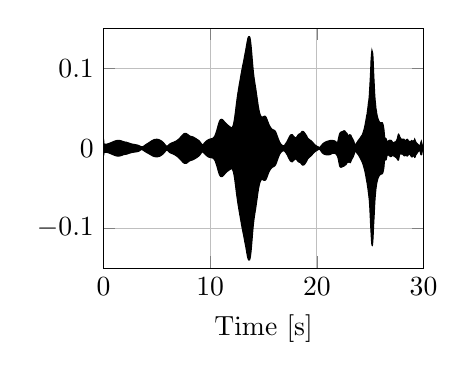
\begin{tikzpicture}

\begin{axis}[%
width=1.6in,
height=1.2in,
at={(0.758in,0.481in)},
scale only axis,
xmin=0,
xmax=30,
xmajorgrids,
ymin=-0.15,
ymax=0.15,
ymajorgrids,
xlabel={Time [s]},
axis background/.style={fill=white}
]
\addplot[fill=black,draw=black,forget plot] plot table[row sep=crcr]{%
2.08333333333333e-05	0.0114785432815552\\
0.0417454218822439	0.00534069538116455\\
0.0834700104311544	0.0052037239074707\\
0.125194598980065	0.00509238243103027\\
0.166919187528975	0.00505948066711426\\
0.208643776077886	0.00505304336547852\\
0.250368364626797	0.00506722927093506\\
0.292092953175707	0.00510072708129883\\
0.333817541724618	0.00517630577087402\\
0.375542130273528	0.00533735752105713\\
0.417266718822439	0.0055391788482666\\
0.458991307371349	0.00569117069244385\\
0.50071589592026	0.00591754913330078\\
0.54244048446917	0.00608587265014648\\
0.584165073018081	0.00630474090576172\\
0.625889661566991	0.00655174255371094\\
0.667614250115902	0.00675761699676514\\
0.709338838664812	0.00699985027313232\\
0.751063427213723	0.00724232196807861\\
0.792788015762633	0.0074760913848877\\
0.834512604311544	0.00767660140991211\\
0.876237192860454	0.00795340538024902\\
0.917961781409365	0.00821197032928467\\
0.959686369958275	0.00845563411712646\\
1.00141095850719	0.00869143009185791\\
1.0431355470561	0.00889706611633301\\
1.08486013560501	0.00906515121459961\\
1.12658472415392	0.00923120975494385\\
1.16830931270283	0.0093923807144165\\
1.21003390125174	0.00953054428100586\\
1.25175848980065	0.00961649417877197\\
1.29348307834956	0.00968992710113525\\
1.33520766689847	0.00975620746612549\\
1.37693225544738	0.00977027416229248\\
1.41865684399629	0.00979197025299072\\
1.4603814325452	0.00975573062896729\\
1.50210602109411	0.00971114635467529\\
1.54383060964302	0.00958013534545898\\
1.58555519819193	0.00945448875427246\\
1.62727978674084	0.00931358337402344\\
1.66900437528975	0.00910115242004395\\
1.71072896383866	0.00893723964691162\\
1.75245355238758	0.00874602794647217\\
1.79417814093649	0.00853836536407471\\
1.8359027294854	0.0083693265914917\\
1.87762731803431	0.00821232795715332\\
1.91935190658322	0.00802934169769287\\
1.96107649513213	0.00789356231689453\\
2.00280108368104	0.00774061679840088\\
2.04452567222995	0.00761866569519043\\
2.08625026077886	0.00758874416351318\\
2.12797484932777	0.00756692886352539\\
2.16969943787668	0.00743842124938965\\
2.21142402642559	0.00719094276428223\\
2.2531486149745	0.00699293613433838\\
2.29487320352341	0.00681674480438232\\
2.33659779207232	0.0066457986831665\\
2.37832238062123	0.00647664070129395\\
2.42004696917014	0.00627219676971436\\
2.46177155771905	0.00604939460754395\\
2.50349614626796	0.00588810443878174\\
2.54522073481687	0.00566399097442627\\
2.58694532336579	0.00548028945922852\\
2.6286699119147	0.00532341003417969\\
2.67039450046361	0.0052030086517334\\
2.71211908901252	0.00507640838623047\\
2.75384367756143	0.00497794151306152\\
2.79556826611034	0.0049053430557251\\
2.83729285465925	0.00479698181152344\\
2.87901744320816	0.00472640991210938\\
2.92074203175707	0.00461506843566895\\
2.96246662030598	0.00450980663299561\\
3.00419120885489	0.0044177770614624\\
3.0459157974038	0.00430214405059814\\
3.08764038595271	0.00418400764465332\\
3.12936497450162	0.0040583610534668\\
3.17108956305053	0.00390028953552246\\
3.21281415159944	0.00372755527496338\\
3.25453874014835	0.00353491306304932\\
3.29626332869726	0.0033574104309082\\
3.33798791724618	0.00312888622283936\\
3.37971250579509	0.00290012359619141\\
3.421437094344	0.00257015228271484\\
3.46316168289291	0.00231432914733887\\
3.50488627144182	0.00214219093322754\\
3.54661085999073	0.00198984146118164\\
3.58833544853964	0.00189602375030518\\
3.63006003708855	0.00188291072845459\\
3.67178462563746	0.00196444988250732\\
3.71350921418637	0.00214886665344238\\
3.75523380273528	0.00245249271392822\\
3.79695839128419	0.00285136699676514\\
3.8386829798331	0.00326979160308838\\
3.88040756838201	0.00369596481323242\\
3.92213215693092	0.00411736965179443\\
3.96385674547983	0.00452029705047607\\
4.00558133402874	0.00487256050109863\\
4.04730592257765	0.0052332878112793\\
4.08903051112656	0.00558674335479736\\
4.13075509967547	0.00593149662017822\\
4.17247968822439	0.0062631368637085\\
4.2142042767733	0.0066298246383667\\
4.25592886532221	0.00696063041687012\\
4.29765345387112	0.00729620456695557\\
4.33937804242003	0.00766825675964355\\
4.38110263096894	0.00801551342010498\\
4.42282721951785	0.00840151309967041\\
4.46455180806676	0.00876975059509277\\
4.50627639661567	0.009147047996521\\
4.54800098516458	0.00947320461273193\\
4.58972557371349	0.00974583625793457\\
4.6314501622624	0.0100482702255249\\
4.67317475081131	0.0103269815444946\\
4.71489933936022	0.0105452537536621\\
4.75662392790913	0.0107525587081909\\
4.79834851645804	0.0108976364135742\\
4.84007310500695	0.011013388633728\\
4.88179769355586	0.0110751390457153\\
4.92352228210478	0.0111459493637085\\
4.96524687065368	0.0111769437789917\\
5.0069714592026	0.0111671686172485\\
5.04869604775151	0.0111480951309204\\
5.09042063630042	0.0110526084899902\\
5.13214522484933	0.0109189748764038\\
5.17386981339824	0.0107687711715698\\
5.21559440194715	0.01054847240448\\
5.25731899049606	0.0103210210800171\\
5.29904357904497	0.0100440979003906\\
5.34076816759388	0.00974357128143311\\
5.38249275614279	0.00941193103790283\\
5.4242173446917	0.00905430316925049\\
5.46594193324061	0.00865852832794189\\
5.50766652178952	0.00818371772766113\\
5.54939111033843	0.00771212577819824\\
5.59111569888734	0.00722098350524902\\
5.63284028743625	0.00662851333618164\\
5.67456487598516	0.00595009326934814\\
5.71628946453407	0.00527417659759521\\
5.75801405308299	0.0045548677444458\\
5.7997386416319	0.00389194488525391\\
5.84146323018081	0.00328123569488525\\
5.88318781872972	0.00275218486785889\\
5.92491240727863	0.00241494178771973\\
5.96663699582754	0.00255095958709717\\
6.00836158437645	0.00294482707977295\\
6.05008617292536	0.00342845916748047\\
6.09181076147427	0.00398170948028564\\
6.13353535002318	0.00448405742645264\\
6.17525993857209	0.00494205951690674\\
6.216984527121	0.00536775588989258\\
6.25870911566991	0.00571024417877197\\
6.30043370421882	0.00602984428405762\\
6.34215829276773	0.00631535053253174\\
6.38388288131664	0.00655972957611084\\
6.42560746986555	0.00681376457214355\\
6.46733205841446	0.00701034069061279\\
6.50905664696338	0.00723159313201904\\
6.55078123551229	0.00743937492370605\\
6.5925058240612	0.00764286518096924\\
6.63423041261011	0.0078728199005127\\
6.67595500115902	0.00812351703643799\\
6.71767958970793	0.00841009616851807\\
6.75940417825684	0.00866270065307617\\
6.80112876680575	0.00895547866821289\\
6.84285335535466	0.0092780590057373\\
6.88457794390357	0.00965094566345215\\
6.92630253245248	0.0100514888763428\\
6.96802712100139	0.0104825496673584\\
7.0097517095503	0.0109357833862305\\
7.05147629809921	0.0114067792892456\\
7.09320088664812	0.0119482278823853\\
7.13492547519703	0.0125249624252319\\
7.17665006374594	0.0130912065505981\\
7.21837465229485	0.0137603282928467\\
7.26009924084376	0.0143387317657471\\
7.30182382939268	0.014959454536438\\
7.34354841794159	0.0155916213989258\\
7.3852730064905	0.0162895917892456\\
7.42699759503941	0.0168346166610718\\
7.46872218358832	0.0173873901367188\\
7.51044677213723	0.0178295373916626\\
7.55217136068614	0.0181968212127686\\
7.59389594923505	0.0184116363525391\\
7.63562053778396	0.0185434818267822\\
7.67734512633287	0.0185559988021851\\
7.71906971488178	0.0184913873672485\\
7.76079430343069	0.0182911157608032\\
7.8025188919796	0.0179351568222046\\
7.84424348052851	0.0176155567169189\\
7.88596806907742	0.0172228813171387\\
7.92769265762633	0.0168032646179199\\
7.96941724617524	0.0163617134094238\\
8.01114183472416	0.0159536600112915\\
8.05286642327307	0.0156121253967285\\
8.09459101182198	0.0153399705886841\\
8.13631560037089	0.01503586769104\\
8.1780401889198	0.0148335695266724\\
8.21976477746871	0.0146785974502563\\
8.26148936601762	0.014529824256897\\
8.30321395456653	0.014382004737854\\
8.34493854311544	0.014241099357605\\
8.38666313166435	0.0140353441238403\\
8.42838772021326	0.013795018196106\\
8.47011230876217	0.0134928226470947\\
8.51183689731108	0.0131955146789551\\
8.55356148585999	0.0128636360168457\\
8.5952860744089	0.0125170946121216\\
8.63701066295781	0.0120959281921387\\
8.67873525150672	0.0118252038955688\\
8.72045984005563	0.0114930868148804\\
8.76218442860454	0.0110743045806885\\
8.80390901715345	0.0107171535491943\\
8.84563360570237	0.0104146003723145\\
8.88735819425128	0.0100103616714478\\
8.92908278280018	0.00954747200012207\\
8.9708073713491	0.00900590419769287\\
9.01253195989801	0.00838887691497803\\
9.05425654844692	0.00773584842681885\\
9.09598113699583	0.00699663162231445\\
9.13770572554474	0.00621140003204346\\
9.17943031409365	0.00548946857452393\\
9.22115490264256	0.00486087799072266\\
9.26287949119147	0.00438857078552246\\
9.30460407974038	0.00439012050628662\\
9.34632866828929	0.0048060417175293\\
9.3880532568382	0.00540995597839355\\
9.42977784538711	0.00605833530426025\\
9.47150243393602	0.00671577453613281\\
9.51322702248493	0.0073617696762085\\
9.55495161103384	0.00787365436553955\\
9.59667619958275	0.00840520858764648\\
9.63840078813166	0.00892412662506104\\
9.68012537668058	0.00935518741607666\\
9.72184996522949	0.00972664356231689\\
9.7635745537784	0.0101182460784912\\
9.80529914232731	0.010441780090332\\
9.84702373087622	0.010714054107666\\
9.88874831942513	0.0110061168670654\\
9.93047290797404	0.0112310647964478\\
9.97219749652295	0.0113784074783325\\
10.0139220850719	0.0115810632705688\\
10.0556466736208	0.0116569995880127\\
10.0973712621697	0.0118051767349243\\
10.1390958507186	0.0118732452392578\\
10.1808204392675	0.0120276212692261\\
10.2225450278164	0.0123337507247925\\
10.2642696163653	0.0126442909240723\\
10.3059942049142	0.0130822658538818\\
10.3477187934631	0.0136831998825073\\
10.3894433820121	0.0144659280776978\\
10.431167970561	0.0154234170913696\\
10.4728925591099	0.0166769027709961\\
10.5146171476588	0.0181429386138916\\
10.5563417362077	0.0197334289550781\\
10.5980663247566	0.0214874744415283\\
10.6397909133055	0.0234543085098267\\
10.6815155018544	0.0254465341567993\\
10.7232400904033	0.0275928974151611\\
10.7649646789523	0.0295801162719727\\
10.8066892675012	0.0313324928283691\\
10.8484138560501	0.0329288244247437\\
10.890138444599	0.0342257022857666\\
10.9318630331479	0.0352087020874023\\
10.9735876216968	0.0358078479766846\\
11.0153122102457	0.0361278057098389\\
11.0570367987946	0.0361744165420532\\
11.0987613873435	0.0360897779464722\\
11.1404859758924	0.0357940196990967\\
11.1822105644414	0.0353696346282959\\
11.2239351529903	0.0348323583602905\\
11.2656597415392	0.0341284275054932\\
11.3073843300881	0.0333702564239502\\
11.349108918637	0.0328712463378906\\
11.3908335071859	0.0322641134262085\\
11.4325580957348	0.0316240787506104\\
11.4742826842837	0.0310574769973755\\
11.5160072728326	0.0304851531982422\\
11.5577318613816	0.0299694538116455\\
11.5994564499305	0.0294324159622192\\
11.6411810384794	0.0289604663848877\\
11.6829056270283	0.0285258293151855\\
11.7246302155772	0.0280790328979492\\
11.7663548041261	0.0276212692260742\\
11.808079392675	0.027173638343811\\
11.8498039812239	0.0267442464828491\\
11.8915285697728	0.0263036489486694\\
11.9332531583217	0.0259977579116821\\
11.9749777468707	0.0257173776626587\\
12.0167023354196	0.0256444215774536\\
12.0584269239685	0.0260707139968872\\
12.1001515125174	0.0268868207931519\\
12.1418761010663	0.0282458066940308\\
12.1836006896152	0.0301697254180908\\
12.2253252781641	0.0328278541564941\\
12.267049866713	0.0361294746398926\\
12.3087744552619	0.0398577451705933\\
12.3504990438108	0.0442241430282593\\
12.3922236323598	0.048554539680481\\
12.4339482209087	0.0533065795898438\\
12.4756728094576	0.0577112436294556\\
12.5173973980065	0.0618079900741577\\
12.5591219865554	0.0658514499664307\\
12.6008465751043	0.0694860219955444\\
12.6425711636532	0.0729827880859375\\
12.6842957522021	0.0762676000595093\\
12.726020340751	0.0796948671340942\\
12.7677449293	0.082758903503418\\
12.8094695178489	0.0858826637268066\\
12.8511941063978	0.0890834331512451\\
12.8929186949467	0.0924304723739624\\
12.9346432834956	0.0954339504241943\\
12.9763678720445	0.0984653234481812\\
13.0180924605934	0.101299405097961\\
13.0598170491423	0.104160785675049\\
13.1015416376912	0.106786608695984\\
13.1432662262401	0.109590768814087\\
13.1849908147891	0.112443804740906\\
13.226715403338	0.115613102912903\\
13.2684399918869	0.118616223335266\\
13.3101645804358	0.121266603469849\\
13.3518891689847	0.124480009078979\\
13.3936137575336	0.12775444984436\\
13.4353383460825	0.130913376808167\\
13.4770629346314	0.133987069129944\\
13.5187875231803	0.13662576675415\\
13.5605121117293	0.138445258140564\\
13.6022367002782	0.139384031295776\\
13.6439612888271	0.139587163925171\\
13.685685877376	0.139370322227478\\
13.7274104659249	0.13790237903595\\
13.7691350544738	0.135053515434265\\
13.8108596430227	0.13035774230957\\
13.8525842315716	0.124771356582642\\
13.8943088201205	0.11833918094635\\
13.9360334086694	0.111524105072021\\
13.9777579972184	0.10494601726532\\
14.0194825857673	0.098751425743103\\
14.0612071743162	0.0933233499526978\\
14.1029317628651	0.0888255834579468\\
14.144656351414	0.084977388381958\\
14.1863809399629	0.0813279151916504\\
14.2281055285118	0.0778927803039551\\
14.2698301170607	0.074398398399353\\
14.3115547056096	0.0705685615539551\\
14.3532792941586	0.0667481422424316\\
14.3950038827075	0.0628595352172852\\
14.4367284712564	0.0587108135223389\\
14.4784530598053	0.0548607110977173\\
14.5201776483542	0.0514167547225952\\
14.5619022369031	0.0482838153839111\\
14.603626825452	0.045663595199585\\
14.6453514140009	0.0435001850128174\\
14.6870760025498	0.0418145656585693\\
14.7288005910988	0.0404582023620605\\
14.7705251796477	0.0396591424942017\\
14.8122497681966	0.0391381978988647\\
14.8539743567455	0.0388869047164917\\
14.8956989452944	0.0389077663421631\\
14.9374235338433	0.0391435623168945\\
14.9791481223922	0.0394853353500366\\
15.0208727109411	0.0397598743438721\\
15.06259729949	0.0399566888809204\\
15.1043218880389	0.0400079488754272\\
15.1460464765879	0.0399395227432251\\
15.1877710651368	0.0395148992538452\\
15.2294956536857	0.0388205051422119\\
15.2712202422346	0.0377287864685059\\
15.3129448307835	0.0364135503768921\\
15.3546694193324	0.0348590612411499\\
15.3963940078813	0.0333253145217896\\
15.4381185964302	0.0319628715515137\\
15.4798431849791	0.0304471254348755\\
15.521567773528	0.0292129516601563\\
15.563292362077	0.0280615091323853\\
15.6050169506259	0.0270326137542725\\
15.6467415391748	0.0261362791061401\\
15.6884661277237	0.0253252983093262\\
15.7301907162726	0.0246288776397705\\
15.7719153048215	0.0240567922592163\\
15.8136398933704	0.0235652923583984\\
15.8553644819193	0.0232577323913574\\
15.8970890704682	0.0230278968811035\\
15.9388136590172	0.0228309631347656\\
15.9805382475661	0.0225493907928467\\
16.022262836115	0.0222042798995972\\
16.0639874246639	0.0217149257659912\\
16.1057120132128	0.0209826231002808\\
16.1474366017617	0.0199587345123291\\
16.1891611903106	0.018677830696106\\
16.2308857788595	0.0172425508499146\\
16.2726103674084	0.0156550407409668\\
16.3143349559573	0.0140594244003296\\
16.3560595445063	0.0124814510345459\\
16.3977841330552	0.0110762119293213\\
16.4395087216041	0.00968575477600098\\
16.481233310153	0.00845015048980713\\
16.5229578987019	0.00733089447021484\\
16.5646824872508	0.00630056858062744\\
16.6064070757997	0.00547575950622559\\
16.6481316643486	0.00478112697601318\\
16.6898562528975	0.00421690940856934\\
16.7315808414465	0.00380945205688477\\
16.7733054299954	0.00352680683135986\\
16.8150300185443	0.00329411029815674\\
16.8567546070932	0.00310599803924561\\
16.8984791956421	0.00304758548736572\\
16.940203784191	0.00325202941894531\\
16.9819283727399	0.00392711162567139\\
17.0236529612888	0.00483942031860352\\
17.0653775498377	0.00562882423400879\\
17.1071021383867	0.00637829303741455\\
17.1488267269356	0.00727784633636475\\
17.1905513154845	0.00809097290039063\\
17.2322759040334	0.00909316539764404\\
17.2740004925823	0.0102552175521851\\
17.3157250811312	0.0114556550979614\\
17.3574496696801	0.0126138925552368\\
17.399174258229	0.0137237310409546\\
17.4408988467779	0.0147284269332886\\
17.4826234353268	0.0155774354934692\\
17.5243480238758	0.0163058042526245\\
17.5660726124247	0.0167961120605469\\
17.6077972009736	0.016975998878479\\
17.6495217895225	0.0170122385025024\\
17.6912463780714	0.016900897026062\\
17.7329709666203	0.0162880420684814\\
17.7746955551692	0.0155270099639893\\
17.8164201437181	0.0150400400161743\\
17.858144732267	0.0143778324127197\\
17.8998693208159	0.0138396024703979\\
17.9415939093649	0.013364315032959\\
17.9833184979138	0.013167142868042\\
18.0250430864627	0.0131821632385254\\
18.0667676750116	0.0135804414749146\\
18.1084922635605	0.014189600944519\\
18.1502168521094	0.0147428512573242\\
18.1919414406583	0.01580810546875\\
18.2336660292072	0.0163758993148804\\
18.2753906177561	0.0172550678253174\\
18.3171152063051	0.0175600051879883\\
18.358839794854	0.0177550315856934\\
18.4005643834029	0.0180671215057373\\
18.4422889719518	0.0182669162750244\\
18.4840135605007	0.0188618898391724\\
18.5257381490496	0.019569993019104\\
18.5674627375985	0.0203806161880493\\
18.6091873261474	0.020946741104126\\
18.6509119146963	0.0210894346237183\\
18.6926365032453	0.0210072994232178\\
18.7343610917942	0.0207293033599854\\
18.7760856803431	0.0203676223754883\\
18.817810268892	0.0197062492370605\\
18.8595348574409	0.0189294815063477\\
18.9012594459898	0.0181183815002441\\
18.9429840345387	0.0172309875488281\\
18.9847086230876	0.0165185928344727\\
19.0264332116365	0.0156053304672241\\
19.0681578001854	0.0144500732421875\\
19.1098823887344	0.0133981704711914\\
19.1516069772833	0.0125586986541748\\
19.1933315658322	0.0119558572769165\\
19.2350561543811	0.0114675760269165\\
19.27678074293	0.0110379457473755\\
19.3185053314789	0.0105326175689697\\
19.3602299200278	0.0100845098495483\\
19.4019545085767	0.00985336303710938\\
19.4436790971256	0.00950038433074951\\
19.4854036856745	0.0090022087097168\\
19.5271282742235	0.00845694541931152\\
19.5688528627724	0.00785517692565918\\
19.6105774513213	0.0072627067565918\\
19.6523020398702	0.00660943984985352\\
19.6940266284191	0.00592970848083496\\
19.735751216968	0.00526082515716553\\
19.7774758055169	0.00465011596679688\\
19.8192003940658	0.00417578220367432\\
19.8609249826147	0.00375926494598389\\
19.9026495711637	0.0033566951751709\\
19.9443741597126	0.00300157070159912\\
19.9860987482615	0.0026402473449707\\
20.0278233368104	0.00230562686920166\\
20.0695479253593	0.00206625461578369\\
20.1112725139082	0.00180244445800781\\
20.1529971024571	0.00143909454345703\\
20.194721691006	0.00109946727752686\\
20.2364462795549	0.000847101211547852\\
20.2781708681038	0.00121331214904785\\
20.3198954566528	0.00177955627441406\\
20.3616200452017	0.00240421295166016\\
20.4033446337506	0.00306963920593262\\
20.4450692222995	0.00374388694763184\\
20.4867938108484	0.00441265106201172\\
20.5285183993973	0.00502192974090576\\
20.5702429879462	0.00559186935424805\\
20.6119675764951	0.00607085227966309\\
20.653692165044	0.00651729106903076\\
20.695416753593	0.00695490837097168\\
20.7371413421419	0.00726485252380371\\
20.7788659306908	0.00762331485748291\\
20.8205905192397	0.00786769390106201\\
20.8623151077886	0.00811982154846191\\
20.9040396963375	0.00837433338165283\\
20.9457642848864	0.0086061954498291\\
20.9874888734353	0.00871777534484863\\
21.0292134619842	0.00885879993438721\\
21.0709380505331	0.00897300243377686\\
21.1126626390821	0.00911998748779297\\
21.154387227631	0.0092850923538208\\
21.1961118161799	0.00943160057067871\\
21.2378364047288	0.00961482524871826\\
21.2795609932777	0.00961482524871826\\
21.3212855818266	0.00966775417327881\\
21.3630101703755	0.00972282886505127\\
21.4047347589244	0.00967347621917725\\
21.4464593474733	0.00967323780059814\\
21.4881839360223	0.00964236259460449\\
21.5299085245712	0.00958514213562012\\
21.5716331131201	0.00948750972747803\\
21.613357701669	0.00936532020568848\\
21.6550822902179	0.00921285152435303\\
21.6968068787668	0.00889825820922852\\
21.7385314673157	0.00858700275421143\\
21.7802560558646	0.00806295871734619\\
21.8219806444135	0.00749027729034424\\
21.8637052329624	0.00666284561157227\\
21.9054298215114	0.00554168224334717\\
21.9471544100603	0.00739622116088867\\
21.9888789986092	0.00995814800262451\\
22.0306035871581	0.0125199556350708\\
22.072328175707	0.0150238275527954\\
22.1140527642559	0.0171887874603271\\
22.1557773528048	0.0185993909835815\\
22.1975019413537	0.0194535255432129\\
22.2392265299026	0.0200250148773193\\
22.2809511184516	0.0201977491378784\\
22.3226757070005	0.0204402208328247\\
22.3644002955494	0.0206606388092041\\
22.4061248840983	0.0209667682647705\\
22.4478494726472	0.0210415124893188\\
22.4895740611961	0.0211354494094849\\
22.531298649745	0.0217199325561523\\
22.5730232382939	0.0212846994400024\\
22.6147478268428	0.0216156244277954\\
22.6564724153917	0.0207544565200806\\
22.6981970039407	0.0202834606170654\\
22.7399215924896	0.0193712711334229\\
22.7816461810385	0.0191372632980347\\
22.8233707695874	0.0184758901596069\\
22.8650953581363	0.0169388055801392\\
22.9068199466852	0.0163617134094238\\
22.9485445352341	0.0162371397018433\\
22.990269123783	0.0158524513244629\\
23.0319937123319	0.0156512260437012\\
23.0737183008809	0.0168333053588867\\
23.1154428894298	0.0166013240814209\\
23.1571674779787	0.0164968967437744\\
23.1988920665276	0.0158416032791138\\
23.2406166550765	0.0143569707870483\\
23.2823412436254	0.0129103660583496\\
23.3240658321743	0.0124514102935791\\
23.3657904207232	0.0114026069641113\\
23.4075150092721	0.0102609395980835\\
23.449239597821	0.00900018215179443\\
23.49096418637	0.00729286670684814\\
23.5326887749189	0.00533103942871094\\
23.5744133634678	0.00352764129638672\\
23.6161379520167	0.00429928302764893\\
23.6578625405656	0.00502634048461914\\
23.6995871291145	0.00603604316711426\\
23.7413117176634	0.00687646865844727\\
23.7830363062123	0.00777220726013184\\
23.8247608947612	0.00861501693725586\\
23.8664854833102	0.00944793224334717\\
23.9082100718591	0.0101504325866699\\
23.949934660408	0.0108531713485718\\
23.9916592489569	0.0115765333175659\\
24.0333838375058	0.0123437643051147\\
24.0751084260547	0.0131453275680542\\
24.1168330146036	0.0139836072921753\\
24.1585576031525	0.0148329734802246\\
24.2002821917014	0.0156471729278564\\
24.2420067802503	0.0164941549301147\\
24.2837313687993	0.017812967300415\\
24.3254559573482	0.0193901062011719\\
24.3671805458971	0.0210870504379272\\
24.408905134446	0.0229474306106567\\
24.4506297229949	0.0251200199127197\\
24.4923543115438	0.0275436639785767\\
24.5340789000927	0.0304191112518311\\
24.5758034886416	0.0334633588790894\\
24.6175280771905	0.0366885662078857\\
24.6592526657395	0.0400806665420532\\
24.7009772542884	0.0425902605056763\\
24.7427018428373	0.0469040870666504\\
24.7844264313862	0.0509792566299438\\
24.8261510199351	0.0560919046401978\\
24.867875608484	0.0594334602355957\\
24.9096001970329	0.0651278495788574\\
24.9513247855818	0.0746465921401978\\
24.9930493741307	0.084429144859314\\
25.0347739626796	0.0951424837112427\\
25.0764985512286	0.109703779220581\\
25.1182231397775	0.117620348930359\\
25.1599477283264	0.12228536605835\\
25.2016723168753	0.120319843292236\\
25.2433969054242	0.117872834205627\\
25.2851214939731	0.106775164604187\\
25.326846082522	0.0924705266952515\\
25.3685706710709	0.0815415382385254\\
25.4102952596198	0.0698156356811523\\
25.4520198481687	0.0612390041351318\\
25.4937444367177	0.056238055229187\\
25.5354690252666	0.0498535633087158\\
25.5771936138155	0.046770453453064\\
25.6189182023644	0.0427716970443726\\
25.6606427909133	0.0401996374130249\\
25.7023673794622	0.0379753112792969\\
25.7440919680111	0.0363017320632935\\
25.78581655656	0.0349266529083252\\
25.8275411451089	0.0337135791778564\\
25.8692657336579	0.0328520536422729\\
25.9109903222068	0.0321235656738281\\
25.9527149107557	0.0317413806915283\\
25.9944394993046	0.0315654277801514\\
26.0361640878535	0.0319061279296875\\
26.0778886764024	0.0319470167160034\\
26.1196132649513	0.0319187641143799\\
26.1613378535002	0.0313384532928467\\
26.2030624420491	0.0294170379638672\\
26.2447870305981	0.0269978046417236\\
26.286511619147	0.0231131315231323\\
26.3282362076959	0.0172504186630249\\
26.3699607962448	0.0116676092147827\\
26.4116853847937	0.0121510028839111\\
26.4534099733426	0.012372612953186\\
26.4951345618915	0.0118190050125122\\
26.5368591504404	0.00980114936828613\\
26.5785837389893	0.00773417949676514\\
26.6203083275383	0.00816822052001953\\
26.6620329160872	0.0087505578994751\\
26.7037575046361	0.00914323329925537\\
26.745482093185	0.00954926013946533\\
26.7872066817339	0.00982666015625\\
26.8289312702828	0.0100194215774536\\
26.8706558588317	0.00991547107696533\\
26.9123804473806	0.00985050201416016\\
26.9541050359295	0.00980710983276367\\
26.9958296244784	0.00945329666137695\\
27.0375542130274	0.00854921340942383\\
27.0792788015763	0.00761783123016357\\
27.1210033901252	0.00674962997436523\\
27.1627279786741	0.00695240497589111\\
27.204452567223	0.00716555118560791\\
27.2461771557719	0.00735676288604736\\
27.2879017443208	0.00772666931152344\\
27.3296263328697	0.00782358646392822\\
27.3713509214186	0.00800633430480957\\
27.4130755099675	0.00846564769744873\\
27.4548000985165	0.009391188621521\\
27.4965246870654	0.0104737281799316\\
27.5382492756143	0.0120096206665039\\
27.5799738641632	0.0143327713012695\\
27.6216984527121	0.0168287754058838\\
27.663423041261	0.017547607421875\\
27.7051476298099	0.0166571140289307\\
27.7468722183588	0.0154355764389038\\
27.7885968069077	0.0137665271759033\\
27.8303213954567	0.0128190517425537\\
27.8720459840056	0.0119119882583618\\
27.9137705725545	0.0114715099334717\\
27.9554951611034	0.011310338973999\\
27.9972197496523	0.0112506151199341\\
28.0389443382012	0.0112757682800293\\
28.0806689267501	0.0114147663116455\\
28.122393515299	0.0114510059356689\\
28.1641181038479	0.0112447738647461\\
28.2058426923968	0.0103377103805542\\
28.2475672809458	0.00945615768432617\\
28.2892918694947	0.00961887836456299\\
28.3310164580436	0.0098271369934082\\
28.3727410465925	0.0102313756942749\\
28.4144656351414	0.0107779502868652\\
28.4561902236903	0.0111668109893799\\
28.4979148122392	0.0111263990402222\\
28.5396394007881	0.0102998018264771\\
28.581363989337	0.00894224643707275\\
28.623088577886	0.0083763599395752\\
28.6648131664349	0.00829541683197021\\
28.7065377549838	0.00867295265197754\\
28.7482623435327	0.00846350193023682\\
28.7899869320816	0.00835263729095459\\
28.8317115206305	0.00910520553588867\\
28.8734361091794	0.00964760780334473\\
28.9151606977283	0.00955963134765625\\
28.9568852862772	0.00906741619110107\\
28.9986098748261	0.00873363018035889\\
29.0403344633751	0.00894296169281006\\
29.082059051924	0.00941741466522217\\
29.1237836404729	0.00970685482025146\\
29.1655082290218	0.0114222764968872\\
29.2072328175707	0.0101405382156372\\
29.2489574061196	0.00831997394561768\\
29.2906819946685	0.00751984119415283\\
29.3324065832174	0.00681853294372559\\
29.3741311717663	0.00610756874084473\\
29.4158557603153	0.00550460815429688\\
29.4575803488642	0.00503480434417725\\
29.4993049374131	0.00431215763092041\\
29.541029525962	0.00394904613494873\\
29.5827541145109	0.00357246398925781\\
29.6244787030598	0.00324690341949463\\
29.6662032916087	0.0031512975692749\\
29.7079278801576	0.0049738883972168\\
29.7496524687065	0.00726950168609619\\
29.7913770572554	0.00879693031311035\\
29.8331016458044	0.00664782524108887\\
29.8748262343533	0.00428330898284912\\
29.9165508229022	0.00285017490386963\\
29.9582754114511	0.00128185749053955\\
30	0.0022885799407959\\
}
\closedcycle;
\addplot[fill=black,draw=black,forget plot] plot table[row sep=crcr]{%
2.08333333333333e-05	-0.00961685180664063\\
0.0417454218822439	-0.00548064708709717\\
0.0834700104311544	-0.00532269477844238\\
0.125194598980065	-0.00526177883148193\\
0.166919187528975	-0.00520026683807373\\
0.208643776077886	-0.00514411926269531\\
0.250368364626797	-0.00513184070587158\\
0.292092953175707	-0.00517666339874268\\
0.333817541724618	-0.00525593757629395\\
0.375542130273528	-0.00536644458770752\\
0.417266718822439	-0.00552749633789063\\
0.458991307371349	-0.00571560859680176\\
0.50071589592026	-0.00589132308959961\\
0.54244048446917	-0.00611734390258789\\
0.584165073018081	-0.00637912750244141\\
0.625889661566991	-0.0065838098526001\\
0.667614250115902	-0.00679552555084229\\
0.709338838664812	-0.00708615779876709\\
0.751063427213723	-0.00729560852050781\\
0.792788015762633	-0.00752139091491699\\
0.834512604311544	-0.00773835182189941\\
0.876237192860454	-0.00800251960754395\\
0.917961781409365	-0.00824081897735596\\
0.959686369958275	-0.00848400592803955\\
1.00141095850719	-0.00870764255523682\\
1.0431355470561	-0.00894033908843994\\
1.08486013560501	-0.00915396213531494\\
1.12658472415392	-0.00927913188934326\\
1.16830931270283	-0.00940811634063721\\
1.21003390125174	-0.00957667827606201\\
1.25175848980065	-0.00969183444976807\\
1.29348307834956	-0.00972604751586914\\
1.33520766689847	-0.0097649097442627\\
1.37693225544738	-0.00977110862731934\\
1.41865684399629	-0.00974869728088379\\
1.4603814325452	-0.0097343921661377\\
1.50210602109411	-0.00962352752685547\\
1.54383060964302	-0.00952279567718506\\
1.58555519819193	-0.0094219446182251\\
1.62727978674084	-0.00927042961120605\\
1.66900437528975	-0.00908136367797852\\
1.71072896383866	-0.00890779495239258\\
1.75245355238758	-0.00867307186126709\\
1.79417814093649	-0.00848650932312012\\
1.8359027294854	-0.00828003883361816\\
1.87762731803431	-0.00807750225067139\\
1.91935190658322	-0.00794112682342529\\
1.96107649513213	-0.00779044628143311\\
2.00280108368104	-0.00763082504272461\\
2.04452567222995	-0.00753676891326904\\
2.08625026077886	-0.00751888751983643\\
2.12797484932777	-0.00749802589416504\\
2.16969943787668	-0.00741159915924072\\
2.21142402642559	-0.00716590881347656\\
2.2531486149745	-0.00698745250701904\\
2.29487320352341	-0.00679922103881836\\
2.33659779207232	-0.0065997838973999\\
2.37832238062123	-0.00640034675598145\\
2.42004696917014	-0.00621461868286133\\
2.46177155771905	-0.00604534149169922\\
2.50349614626796	-0.00587248802185059\\
2.54522073481687	-0.00571644306182861\\
2.58694532336579	-0.00555884838104248\\
2.6286699119147	-0.00540471076965332\\
2.67039450046361	-0.00530672073364258\\
2.71211908901252	-0.00519084930419922\\
2.75384367756143	-0.00513947010040283\\
2.79556826611034	-0.00501847267150879\\
2.83729285465925	-0.00494086742401123\\
2.87901744320816	-0.00485873222351074\\
2.92074203175707	-0.00477433204650879\\
2.96246662030598	-0.00469052791595459\\
3.00419120885489	-0.00462794303894043\\
3.0459157974038	-0.00453281402587891\\
3.08764038595271	-0.00444555282592773\\
3.12936497450162	-0.00438666343688965\\
3.17108956305053	-0.00421690940856934\\
3.21281415159944	-0.00407671928405762\\
3.25453874014835	-0.00391769409179688\\
3.29626332869726	-0.00369000434875488\\
3.33798791724618	-0.00343704223632813\\
3.37971250579509	-0.00314128398895264\\
3.421437094344	-0.00267946720123291\\
3.46316168289291	-0.00230050086975098\\
3.50488627144182	-0.00197219848632813\\
3.54661085999073	-0.00166225433349609\\
3.58833544853964	-0.00158262252807617\\
3.63006003708855	-0.0018390417098999\\
3.67178462563746	-0.00214171409606934\\
3.71350921418637	-0.00252640247344971\\
3.75523380273528	-0.00293266773223877\\
3.79695839128419	-0.00328266620635986\\
3.8386829798331	-0.00368571281433105\\
3.88040756838201	-0.00402176380157471\\
3.92213215693092	-0.00439083576202393\\
3.96385674547983	-0.00469887256622314\\
4.00558133402874	-0.00502467155456543\\
4.04730592257765	-0.00534725189208984\\
4.08903051112656	-0.00562882423400879\\
4.13075509967547	-0.00594425201416016\\
4.17247968822439	-0.00626230239868164\\
4.2142042767733	-0.00660026073455811\\
4.25592886532221	-0.00689399242401123\\
4.29765345387112	-0.00722026824951172\\
4.33937804242003	-0.00755906105041504\\
4.38110263096894	-0.00786900520324707\\
4.42282721951785	-0.00819563865661621\\
4.46455180806676	-0.00854527950286865\\
4.50627639661567	-0.00883579254150391\\
4.54800098516458	-0.00919878482818604\\
4.58972557371349	-0.00946664810180664\\
4.6314501622624	-0.00970697402954102\\
4.67317475081131	-0.00996339321136475\\
4.71489933936022	-0.0102250576019287\\
4.75662392790913	-0.0103757381439209\\
4.79834851645804	-0.0105174779891968\\
4.84007310500695	-0.0105781555175781\\
4.88179769355586	-0.0106289386749268\\
4.92352228210478	-0.0106924772262573\\
4.96524687065368	-0.0107362270355225\\
5.0069714592026	-0.0107225179672241\\
5.04869604775151	-0.010654091835022\\
5.09042063630042	-0.0105965137481689\\
5.13214522484933	-0.0104855298995972\\
5.17386981339824	-0.0103510618209839\\
5.21559440194715	-0.01020348072052\\
5.25731899049606	-0.00998592376708984\\
5.29904357904497	-0.00973355770111084\\
5.34076816759388	-0.00942492485046387\\
5.38249275614279	-0.00909602642059326\\
5.4242173446917	-0.00875389575958252\\
5.46594193324061	-0.00834751129150391\\
5.50766652178952	-0.00788486003875732\\
5.54939111033843	-0.00744140148162842\\
5.59111569888734	-0.00698447227478027\\
5.63284028743625	-0.00639533996582031\\
5.67456487598516	-0.00575613975524902\\
5.71628946453407	-0.00514018535614014\\
5.75801405308299	-0.00444424152374268\\
5.7997386416319	-0.00371742248535156\\
5.84146323018081	-0.00305914878845215\\
5.88318781872972	-0.00244832038879395\\
5.92491240727863	-0.00217008590698242\\
5.96663699582754	-0.00245964527130127\\
6.00836158437645	-0.00296568870544434\\
6.05008617292536	-0.00349390506744385\\
6.09181076147427	-0.00404369831085205\\
6.13353535002318	-0.00454485416412354\\
6.17525993857209	-0.00498580932617188\\
6.216984527121	-0.00536465644836426\\
6.25870911566991	-0.00572645664215088\\
6.30043370421882	-0.00601232051849365\\
6.34215829276773	-0.00625336170196533\\
6.38388288131664	-0.00647377967834473\\
6.42560746986555	-0.00667273998260498\\
6.46733205841446	-0.00691187381744385\\
6.50905664696338	-0.00712454319000244\\
6.55078123551229	-0.00738382339477539\\
6.5925058240612	-0.00766706466674805\\
6.63423041261011	-0.007973313331604\\
6.67595500115902	-0.00827527046203613\\
6.71767958970793	-0.00860071182250977\\
6.75940417825684	-0.00895512104034424\\
6.80112876680575	-0.00933182239532471\\
6.84285335535466	-0.00968599319458008\\
6.88457794390357	-0.010079026222229\\
6.92630253245248	-0.0104438066482544\\
6.96802712100139	-0.0109328031539917\\
7.0097517095503	-0.0114513635635376\\
7.05147629809921	-0.0119510889053345\\
7.09320088664812	-0.0124548673629761\\
7.13492547519703	-0.0130248069763184\\
7.17665006374594	-0.0136104822158813\\
7.21837465229485	-0.0142343044281006\\
7.26009924084376	-0.0149152278900146\\
7.30182382939268	-0.0155173540115356\\
7.34354841794159	-0.0160833597183228\\
7.3852730064905	-0.0167273283004761\\
7.42699759503941	-0.0172858238220215\\
7.46872218358832	-0.0177969932556152\\
7.51044677213723	-0.0182859897613525\\
7.55217136068614	-0.0186260938644409\\
7.59389594923505	-0.0189026594161987\\
7.63562053778396	-0.0189920663833618\\
7.67734512633287	-0.0190120935440063\\
7.71906971488178	-0.0189443826675415\\
7.76079430343069	-0.0187724828720093\\
7.8025188919796	-0.0185000896453857\\
7.84424348052851	-0.0180740356445313\\
7.88596806907742	-0.0176948308944702\\
7.92769265762633	-0.0172162055969238\\
7.96941724617524	-0.0167680978775024\\
8.01114183472416	-0.0163745880126953\\
8.05286642327307	-0.0159765481948853\\
8.09459101182198	-0.0156924724578857\\
8.13631560037089	-0.0154341459274292\\
8.1780401889198	-0.0152627229690552\\
8.21976477746871	-0.0150817632675171\\
8.26148936601762	-0.0149544477462769\\
8.30321395456653	-0.0147771835327148\\
8.34493854311544	-0.0145810842514038\\
8.38666313166435	-0.0143626928329468\\
8.42838772021326	-0.0141198635101318\\
8.47011230876217	-0.0138207674026489\\
8.51183689731108	-0.0134966373443604\\
8.55356148585999	-0.0131518840789795\\
8.5952860744089	-0.012842059135437\\
8.63701066295781	-0.012513279914856\\
8.67873525150672	-0.0121563673019409\\
8.72045984005563	-0.0118252038955688\\
8.76218442860454	-0.0114935636520386\\
8.80390901715345	-0.011054515838623\\
8.84563360570237	-0.0106476545333862\\
8.88735819425128	-0.0101888179779053\\
8.92908278280018	-0.00979709625244141\\
8.9708073713491	-0.00919747352600098\\
9.01253195989801	-0.00860381126403809\\
9.05425654844692	-0.00785183906555176\\
9.09598113699583	-0.00710380077362061\\
9.13770572554474	-0.00629174709320068\\
9.17943031409365	-0.00555169582366943\\
9.22115490264256	-0.0049283504486084\\
9.26287949119147	-0.00440895557403564\\
9.30460407974038	-0.00453364849090576\\
9.34632866828929	-0.00499343872070313\\
9.3880532568382	-0.00559830665588379\\
9.42977784538711	-0.0062333345413208\\
9.47150243393602	-0.00692856311798096\\
9.51322702248493	-0.00749599933624268\\
9.55495161103384	-0.00804722309112549\\
9.59667619958275	-0.00854074954986572\\
9.63840078813166	-0.00905048847198486\\
9.68012537668058	-0.00949192047119141\\
9.72184996522949	-0.00991165637969971\\
9.7635745537784	-0.0103378295898438\\
9.80529914232731	-0.0106536149978638\\
9.84702373087622	-0.0109461545944214\\
9.88874831942513	-0.0111968517303467\\
9.93047290797404	-0.0114191770553589\\
9.97219749652295	-0.0115553140640259\\
10.0139220850719	-0.01171875\\
10.0556466736208	-0.0117646455764771\\
10.0973712621697	-0.0118610858917236\\
10.1390958507186	-0.011938214302063\\
10.1808204392675	-0.0120800733566284\\
10.2225450278164	-0.012221097946167\\
10.2642696163653	-0.0124901533126831\\
10.3059942049142	-0.012925386428833\\
10.3477187934631	-0.0134956836700439\\
10.3894433820121	-0.0142142772674561\\
10.431167970561	-0.0151938199996948\\
10.4728925591099	-0.016349196434021\\
10.5146171476588	-0.0177477598190308\\
10.5563417362077	-0.0194025039672852\\
10.5980663247566	-0.021106481552124\\
10.6397909133055	-0.0229949951171875\\
10.6815155018544	-0.0249470472335815\\
10.7232400904033	-0.0269877910614014\\
10.7649646789523	-0.0290277004241943\\
10.8066892675012	-0.0307983160018921\\
10.8484138560501	-0.0323613882064819\\
10.890138444599	-0.0336012840270996\\
10.9318630331479	-0.0345585346221924\\
10.9735876216968	-0.035214900970459\\
11.0153122102457	-0.0355126857757568\\
11.0570367987946	-0.035578727722168\\
11.0987613873435	-0.0355178117752075\\
11.1404859758924	-0.0352240800857544\\
11.1822105644414	-0.0348083972930908\\
11.2239351529903	-0.034314751625061\\
11.2656597415392	-0.0336577892303467\\
11.3073843300881	-0.0329146385192871\\
11.349108918637	-0.0323460102081299\\
11.3908335071859	-0.0316728353500366\\
11.4325580957348	-0.0310583114624023\\
11.4742826842837	-0.0304688215255737\\
11.5160072728326	-0.0299209356307983\\
11.5577318613816	-0.0294257402420044\\
11.5994564499305	-0.0289726257324219\\
11.6411810384794	-0.0285561084747314\\
11.6829056270283	-0.0281386375427246\\
11.7246302155772	-0.0277546644210815\\
11.7663548041261	-0.0273803472518921\\
11.808079392675	-0.026955246925354\\
11.8498039812239	-0.026558518409729\\
11.8915285697728	-0.0262095928192139\\
11.9332531583217	-0.025854229927063\\
11.9749777468707	-0.0256175994873047\\
12.0167023354196	-0.02568519115448\\
12.0584269239685	-0.0261075496673584\\
12.1001515125174	-0.0269854068756104\\
12.1418761010663	-0.0283739566802979\\
12.1836006896152	-0.0303318500518799\\
12.2253252781641	-0.0329583883285522\\
12.267049866713	-0.0362371206283569\\
12.3087744552619	-0.0400735139846802\\
12.3504990438108	-0.0443347692489624\\
12.3922236323598	-0.048650860786438\\
12.4339482209087	-0.0532985925674438\\
12.4756728094576	-0.0577074289321899\\
12.5173973980065	-0.0617043972015381\\
12.5591219865554	-0.0657445192337036\\
12.6008465751043	-0.069382905960083\\
12.6425711636532	-0.0729454755783081\\
12.6842957522021	-0.0761911869049072\\
12.726020340751	-0.079504132270813\\
12.7677449293	-0.0827367305755615\\
12.8094695178489	-0.0859740972518921\\
12.8511941063978	-0.0891417264938354\\
12.8929186949467	-0.0922564268112183\\
12.9346432834956	-0.0954611301422119\\
12.9763678720445	-0.0985590219497681\\
13.0180924605934	-0.101478338241577\\
13.0598170491423	-0.104286432266235\\
13.1015416376912	-0.107004284858704\\
13.1432662262401	-0.109845995903015\\
13.1849908147891	-0.112705826759338\\
13.226715403338	-0.11584198474884\\
13.2684399918869	-0.118888258934021\\
13.3101645804358	-0.121429324150085\\
13.3518891689847	-0.124707818031311\\
13.3936137575336	-0.128007292747498\\
13.4353383460825	-0.131151676177979\\
13.4770629346314	-0.134209156036377\\
13.5187875231803	-0.136834263801575\\
13.5605121117293	-0.138666272163391\\
13.6022367002782	-0.139623880386353\\
13.6439612888271	-0.139791250228882\\
13.685685877376	-0.139584302902222\\
13.7274104659249	-0.138070464134216\\
13.7691350544738	-0.135191321372986\\
13.8108596430227	-0.13095498085022\\
13.8525842315716	-0.12542998790741\\
13.8943088201205	-0.118886947631836\\
13.9360334086694	-0.111963868141174\\
13.9777579972184	-0.104978561401367\\
14.0194825857673	-0.0989078283309937\\
14.0612071743162	-0.0934721231460571\\
14.1029317628651	-0.0888721942901611\\
14.144656351414	-0.084964394569397\\
14.1863809399629	-0.081384539604187\\
14.2281055285118	-0.0778763294219971\\
14.2698301170607	-0.0744034051895142\\
14.3115547056096	-0.0705578327178955\\
14.3532792941586	-0.0667208433151245\\
14.3950038827075	-0.0627057552337646\\
14.4367284712564	-0.0586391687393188\\
14.4784530598053	-0.0547771453857422\\
14.5201776483542	-0.0513361692428589\\
14.5619022369031	-0.0481935739517212\\
14.603626825452	-0.045619010925293\\
14.6453514140009	-0.0434579849243164\\
14.6870760025498	-0.0418229103088379\\
14.7288005910988	-0.0406397581100464\\
14.7705251796477	-0.0397793054580688\\
14.8122497681966	-0.0392652750015259\\
14.8539743567455	-0.0390474796295166\\
14.8956989452944	-0.0391877889633179\\
14.9374235338433	-0.0394301414489746\\
14.9791481223922	-0.0396996736526489\\
15.0208727109411	-0.0400179624557495\\
15.06259729949	-0.0401105880737305\\
15.1043218880389	-0.0401661396026611\\
15.1460464765879	-0.0400573015213013\\
15.1877710651368	-0.0396482944488525\\
15.2294956536857	-0.0388807058334351\\
15.2712202422346	-0.0377635955810547\\
15.3129448307835	-0.0363906621932983\\
15.3546694193324	-0.0349268913269043\\
15.3963940078813	-0.0333342552185059\\
15.4381185964302	-0.031851053237915\\
15.4798431849791	-0.0305062532424927\\
15.521567773528	-0.0292800664901733\\
15.563292362077	-0.0282032489776611\\
15.6050169506259	-0.0272564888000488\\
15.6467415391748	-0.0263823270797729\\
15.6884661277237	-0.0256110429763794\\
15.7301907162726	-0.0249224901199341\\
15.7719153048215	-0.0243375301361084\\
15.8136398933704	-0.0238388776779175\\
15.8553644819193	-0.0235472917556763\\
15.8970890704682	-0.0232535600662231\\
15.9388136590172	-0.0229678153991699\\
15.9805382475661	-0.0226802825927734\\
16.022262836115	-0.0222972631454468\\
16.0639874246639	-0.02178955078125\\
16.1057120132128	-0.021040678024292\\
16.1474366017617	-0.0200163125991821\\
16.1891611903106	-0.0187300443649292\\
16.2308857788595	-0.0172457695007324\\
16.2726103674084	-0.0156704187393188\\
16.3143349559573	-0.0140677690505981\\
16.3560595445063	-0.0125261545181274\\
16.3977841330552	-0.011017918586731\\
16.4395087216041	-0.00968563556671143\\
16.481233310153	-0.00843226909637451\\
16.5229578987019	-0.00734817981719971\\
16.5646824872508	-0.00635576248168945\\
16.6064070757997	-0.00551235675811768\\
16.6481316643486	-0.00482070446014404\\
16.6898562528975	-0.00426566600799561\\
16.7315808414465	-0.00388360023498535\\
16.7733054299954	-0.00359523296356201\\
16.8150300185443	-0.00339615345001221\\
16.8567546070932	-0.00323069095611572\\
16.8984791956421	-0.00309169292449951\\
16.940203784191	-0.00309920310974121\\
16.9819283727399	-0.00368702411651611\\
17.0236529612888	-0.00454080104827881\\
17.0653775498377	-0.00525009632110596\\
17.1071021383867	-0.00597429275512695\\
17.1488267269356	-0.00691390037536621\\
17.1905513154845	-0.00776350498199463\\
17.2322759040334	-0.00869929790496826\\
17.2740004925823	-0.00987541675567627\\
17.3157250811312	-0.011139988899231\\
17.3574496696801	-0.0122569799423218\\
17.399174258229	-0.0133496522903442\\
17.4408988467779	-0.0143189430236816\\
17.4826234353268	-0.0152186155319214\\
17.5243480238758	-0.0159556865692139\\
17.5660726124247	-0.0164626836776733\\
17.6077972009736	-0.0167889595031738\\
17.6495217895225	-0.0168652534484863\\
17.6912463780714	-0.016878604888916\\
17.7329709666203	-0.0163320302963257\\
17.7746955551692	-0.0156917572021484\\
17.8164201437181	-0.0153783559799194\\
17.858144732267	-0.0147607326507568\\
17.8998693208159	-0.0142625570297241\\
17.9415939093649	-0.0137666463851929\\
17.9833184979138	-0.0135478973388672\\
18.0250430864627	-0.013524055480957\\
18.0667676750116	-0.0138903856277466\\
18.1084922635605	-0.0144224166870117\\
18.1502168521094	-0.0148800611495972\\
18.1919414406583	-0.0157939195632935\\
18.2336660292072	-0.016310453414917\\
18.2753906177561	-0.0169538259506226\\
18.3171152063051	-0.0173317193984985\\
18.358839794854	-0.017555832862854\\
18.4005643834029	-0.0177218914031982\\
18.4422889719518	-0.0179351568222046\\
18.4840135605007	-0.0184391736984253\\
18.5257381490496	-0.019214391708374\\
18.5674627375985	-0.0200959444046021\\
18.6091873261474	-0.0207067728042603\\
18.6509119146963	-0.0210292339324951\\
18.6926365032453	-0.0210373401641846\\
18.7343610917942	-0.020953893661499\\
18.7760856803431	-0.020803689956665\\
18.817810268892	-0.0204175710678101\\
18.8595348574409	-0.01978600025177\\
18.9012594459898	-0.0189628601074219\\
18.9429840345387	-0.0181024074554443\\
18.9847086230876	-0.0173580646514893\\
19.0264332116365	-0.0163843631744385\\
19.0681578001854	-0.015230655670166\\
19.1098823887344	-0.0140590667724609\\
19.1516069772833	-0.0131498575210571\\
19.1933315658322	-0.0126379728317261\\
19.2350561543811	-0.0120429992675781\\
19.27678074293	-0.0116097927093506\\
19.3185053314789	-0.010983943939209\\
19.3602299200278	-0.0105443000793457\\
19.4019545085767	-0.0101152658462524\\
19.4436790971256	-0.00971567630767822\\
19.4854036856745	-0.00909185409545898\\
19.5271282742235	-0.00846469402313232\\
19.5688528627724	-0.00776255130767822\\
19.6105774513213	-0.00708794593811035\\
19.6523020398702	-0.00646042823791504\\
19.6940266284191	-0.00586962699890137\\
19.735751216968	-0.00526010990142822\\
19.7774758055169	-0.0047677755355835\\
19.8192003940658	-0.0044097900390625\\
19.8609249826147	-0.00407552719116211\\
19.9026495711637	-0.00364327430725098\\
19.9443741597126	-0.00327610969543457\\
19.9860987482615	-0.0029456615447998\\
20.0278233368104	-0.00252127647399902\\
20.0695479253593	-0.0022662878036499\\
20.1112725139082	-0.00191080570220947\\
20.1529971024571	-0.00150704383850098\\
20.194721691006	-0.00117909908294678\\
20.2364462795549	-0.00113403797149658\\
20.2781708681038	-0.00152623653411865\\
20.3198954566528	-0.00227141380310059\\
20.3616200452017	-0.0030587911605835\\
20.4033446337506	-0.00390493869781494\\
20.4450692222995	-0.00472939014434814\\
20.4867938108484	-0.00541806221008301\\
20.5285183993973	-0.00600767135620117\\
20.5702429879462	-0.00648868083953857\\
20.6119675764951	-0.00688314437866211\\
20.653692165044	-0.00721645355224609\\
20.695416753593	-0.00750267505645752\\
20.7371413421419	-0.00771784782409668\\
20.7788659306908	-0.00788450241088867\\
20.8205905192397	-0.00807631015777588\\
20.8623151077886	-0.00811302661895752\\
20.9040396963375	-0.00821447372436523\\
20.9457642848864	-0.00828444957733154\\
20.9874888734353	-0.00830340385437012\\
21.0292134619842	-0.0082862377166748\\
21.0709380505331	-0.00824368000030518\\
21.1126626390821	-0.00819194316864014\\
21.154387227631	-0.00815021991729736\\
21.1961118161799	-0.00803506374359131\\
21.2378364047288	-0.00791525840759277\\
21.2795609932777	-0.0076669454574585\\
21.3212855818266	-0.00736165046691895\\
21.3630101703755	-0.00703608989715576\\
21.4047347589244	-0.00672483444213867\\
21.4464593474733	-0.006492018699646\\
21.4881839360223	-0.00633108615875244\\
21.5299085245712	-0.0062568187713623\\
21.5716331131201	-0.00624167919158936\\
21.613357701669	-0.00627756118774414\\
21.6550822902179	-0.00636100769042969\\
21.6968068787668	-0.00654768943786621\\
21.7385314673157	-0.00679373741149902\\
21.7802560558646	-0.00718104839324951\\
21.8219806444135	-0.00780510902404785\\
21.8637052329624	-0.00851285457611084\\
21.9054298215114	-0.00949275493621826\\
21.9471544100603	-0.0107357501983643\\
21.9888789986092	-0.0126191377639771\\
22.0306035871581	-0.0152097940444946\\
22.072328175707	-0.0182663202285767\\
22.1140527642559	-0.0210949182510376\\
22.1557773528048	-0.0229042768478394\\
22.1975019413537	-0.0235544443130493\\
22.2392265299026	-0.0237547159194946\\
22.2809511184516	-0.023750901222229\\
22.3226757070005	-0.0235217809677124\\
22.3644002955494	-0.0233371257781982\\
22.4061248840983	-0.0227565765380859\\
22.4478494726472	-0.0227081775665283\\
22.4895740611961	-0.022587776184082\\
22.531298649745	-0.0223186016082764\\
22.5730232382939	-0.0220222473144531\\
22.6147478268428	-0.0210109949111938\\
22.6564724153917	-0.0211532115936279\\
22.6981970039407	-0.0208098888397217\\
22.7399215924896	-0.0203430652618408\\
22.7816461810385	-0.0190470218658447\\
22.8233707695874	-0.0179314613342285\\
22.8650953581363	-0.0176577568054199\\
22.9068199466852	-0.0178183317184448\\
22.9485445352341	-0.0174648761749268\\
22.990269123783	-0.0174473524093628\\
23.0319937123319	-0.017309308052063\\
23.0737183008809	-0.0176663398742676\\
23.1154428894298	-0.018006443977356\\
23.1571674779787	-0.0175012350082397\\
23.1988920665276	-0.0159779787063599\\
23.2406166550765	-0.0146782398223877\\
23.2823412436254	-0.0133696794509888\\
23.3240658321743	-0.0125448703765869\\
23.3657904207232	-0.0116766691207886\\
23.4075150092721	-0.0104120969772339\\
23.449239597821	-0.00917649269104004\\
23.49096418637	-0.00768113136291504\\
23.5326887749189	-0.00577187538146973\\
23.5744133634678	-0.00403428077697754\\
23.6161379520167	-0.00322926044464111\\
23.6578625405656	-0.00399744510650635\\
23.6995871291145	-0.00496470928192139\\
23.7413117176634	-0.00578951835632324\\
23.7830363062123	-0.00653350353240967\\
23.8247608947612	-0.00719761848449707\\
23.8664854833102	-0.00784778594970703\\
23.9082100718591	-0.00871062278747559\\
23.949934660408	-0.00967931747436523\\
23.9916592489569	-0.0106616020202637\\
24.0333838375058	-0.0116361379623413\\
24.0751084260547	-0.0127267837524414\\
24.1168330146036	-0.0137753486633301\\
24.1585576031525	-0.0148196220397949\\
24.2002821917014	-0.0159202814102173\\
24.2420067802503	-0.0172525644302368\\
24.2837313687993	-0.0187249183654785\\
24.3254559573482	-0.0203307867050171\\
24.3671805458971	-0.0222201347351074\\
24.408905134446	-0.0241444110870361\\
24.4506297229949	-0.0261446237564087\\
24.4923543115438	-0.028408408164978\\
24.5340789000927	-0.0309720039367676\\
24.5758034886416	-0.0337235927581787\\
24.6175280771905	-0.0370627641677856\\
24.6592526657395	-0.0404403209686279\\
24.7009772542884	-0.0430024862289429\\
24.7427018428373	-0.0470679998397827\\
24.7844264313862	-0.050578236579895\\
24.8261510199351	-0.0550993680953979\\
24.867875608484	-0.0594644546508789\\
24.9096001970329	-0.0642629861831665\\
24.9513247855818	-0.0718753337860107\\
24.9930493741307	-0.0832065343856812\\
25.0347739626796	-0.0949996709823608\\
25.0764985512286	-0.105405926704407\\
25.1182231397775	-0.115448594093323\\
25.1599477283264	-0.121063828468323\\
25.2016723168753	-0.121512651443481\\
25.2433969054242	-0.116709470748901\\
25.2851214939731	-0.10642147064209\\
25.326846082522	-0.0939890146255493\\
25.3685706710709	-0.084175705909729\\
25.4102952596198	-0.0726164579391479\\
25.4520198481687	-0.0627641677856445\\
25.4937444367177	-0.0565850734710693\\
25.5354690252666	-0.0508726835250854\\
25.5771936138155	-0.0467383861541748\\
25.6189182023644	-0.0432323217391968\\
25.6606427909133	-0.0408799648284912\\
25.7023673794622	-0.0388247966766357\\
25.7440919680111	-0.0370969772338867\\
25.78581655656	-0.0357166528701782\\
25.8275411451089	-0.0347107648849487\\
25.8692657336579	-0.0338729619979858\\
25.9109903222068	-0.0333089828491211\\
25.9527149107557	-0.0328136682510376\\
25.9944394993046	-0.0324184894561768\\
26.0361640878535	-0.0323822498321533\\
26.0778886764024	-0.0322884321212769\\
26.1196132649513	-0.0318645238876343\\
26.1613378535002	-0.0311781167984009\\
26.2030624420491	-0.029654860496521\\
26.2447870305981	-0.0271884202957153\\
26.286511619147	-0.0235627889633179\\
26.3282362076959	-0.0168306827545166\\
26.3699607962448	-0.0131574869155884\\
26.4116853847937	-0.0142600536346436\\
26.4534099733426	-0.0146228075027466\\
26.4951345618915	-0.0143215656280518\\
26.5368591504404	-0.0116524696350098\\
26.5785837389893	-0.00919163227081299\\
26.6203083275383	-0.00863409042358398\\
26.6620329160872	-0.00861036777496338\\
26.7037575046361	-0.00844931602478027\\
26.745482093185	-0.00860047340393066\\
26.7872066817339	-0.00919950008392334\\
26.8289312702828	-0.00976109504699707\\
26.8706558588317	-0.0102018117904663\\
26.9123804473806	-0.0104771852493286\\
26.9541050359295	-0.0104862451553345\\
26.9958296244784	-0.0101262331008911\\
27.0375542130274	-0.00962686538696289\\
27.0792788015763	-0.00897753238677979\\
27.1210033901252	-0.00894665718078613\\
27.1627279786741	-0.00937676429748535\\
27.204452567223	-0.00963139533996582\\
27.2461771557719	-0.00999224185943604\\
27.2879017443208	-0.0103377103805542\\
27.3296263328697	-0.0107734203338623\\
27.3713509214186	-0.0110929012298584\\
27.4130755099675	-0.011522650718689\\
27.4548000985165	-0.0119335651397705\\
27.4965246870654	-0.0126463174819946\\
27.5382492756143	-0.0136346817016602\\
27.5799738641632	-0.0146406888961792\\
27.6216984527121	-0.0148977041244507\\
27.663423041261	-0.0143449306488037\\
27.7051476298099	-0.0112202167510986\\
27.7468722183588	-0.00851655006408691\\
27.7885968069077	-0.00694656372070313\\
27.8303213954567	-0.00694513320922852\\
27.8720459840056	-0.007132887840271\\
27.9137705725545	-0.00724780559539795\\
27.9554951611034	-0.00721931457519531\\
27.9972197496523	-0.00735962390899658\\
28.0389443382012	-0.0075448751449585\\
28.0806689267501	-0.00792241096496582\\
28.122393515299	-0.008658766746521\\
28.1641181038479	-0.00931763648986816\\
28.2058426923968	-0.00951695442199707\\
28.2475672809458	-0.00929999351501465\\
28.2892918694947	-0.00879073143005371\\
28.3310164580436	-0.00910067558288574\\
28.3727410465925	-0.00919544696807861\\
28.4144656351414	-0.00951159000396729\\
28.4561902236903	-0.00977611541748047\\
28.4979148122392	-0.00962710380554199\\
28.5396394007881	-0.00884401798248291\\
28.581363989337	-0.0078589916229248\\
28.623088577886	-0.00768864154815674\\
28.6648131664349	-0.00739419460296631\\
28.7065377549838	-0.00783133506774902\\
28.7482623435327	-0.00823354721069336\\
28.7899869320816	-0.00920212268829346\\
28.8317115206305	-0.0100460052490234\\
28.8734361091794	-0.010617733001709\\
28.9151606977283	-0.0109328031539917\\
28.9568852862772	-0.0106092691421509\\
28.9986098748261	-0.00985908508300781\\
29.0403344633751	-0.00975155830383301\\
29.082059051924	-0.00981879234313965\\
29.1237836404729	-0.00995934009552002\\
29.1655082290218	-0.0114542245864868\\
29.2072328175707	-0.0110992193222046\\
29.2489574061196	-0.00927889347076416\\
29.2906819946685	-0.00806748867034912\\
29.3324065832174	-0.00740206241607666\\
29.3741311717663	-0.00656676292419434\\
29.4158557603153	-0.0057758092880249\\
29.4575803488642	-0.00477135181427002\\
29.4993049374131	-0.00423109531402588\\
29.541029525962	-0.00357186794281006\\
29.5827541145109	-0.00324928760528564\\
29.6244787030598	-0.00265228748321533\\
29.6662032916087	-0.00277626514434814\\
29.7079278801576	-0.00583112239837646\\
29.7496524687065	-0.00793993473052979\\
29.7913770572554	-0.00811100006103516\\
29.8331016458044	-0.00761830806732178\\
29.8748262343533	-0.00380218029022217\\
29.9165508229022	-0.00277197360992432\\
29.9582754114511	-0.00150489807128906\\
30	-0.000876903533935547\\
}
\closedcycle;
\end{axis}
\end{tikzpicture}%
	\caption{Vibration from enclosure.}
	\label{fig:raw_enclosure10}
\end{subfigure}
\begin{subfigure}[t]{0.3\textwidth}
	\tikzsetnextfilename{Raw_microphone10}
	% This file was created by matlab2tikz.
%
%The latest updates can be retrieved from
%  http://www.mathworks.com/matlabcentral/fileexchange/22022-matlab2tikz-matlab2tikz
%where you can also make suggestions and rate matlab2tikz.
%
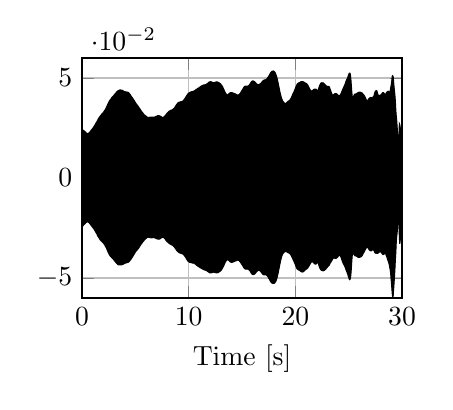
\begin{tikzpicture}

\begin{axis}[%
width=1.6in,
height=1.2in,
at={(0.758in,0.481in)},
scale only axis,
xlabel={Time [s]},
xmin=0,
xmax=30,
xmajorgrids,
ymin=-0.06,
ymax=0.06,
ymajorgrids,
axis background/.style={fill=white}
]
\addplot[fill=black,draw=black,forget plot] plot table[row sep=crcr]{%
2.08333333333333e-05	0.0279340744018555\\
0.0417454218822439	0.0240871906280518\\
0.0834700104311544	0.023901104927063\\
0.125194598980065	0.023756742477417\\
0.166919187528975	0.0236340761184692\\
0.208643776077886	0.0234596729278564\\
0.250368364626797	0.0232491493225098\\
0.292092953175707	0.0230233669281006\\
0.333817541724618	0.0227972269058228\\
0.375542130273528	0.0226085186004639\\
0.417266718822439	0.0224242210388184\\
0.458991307371349	0.022255539894104\\
0.50071589592026	0.0221016407012939\\
0.54244048446917	0.0220683813095093\\
0.584165073018081	0.0221813917160034\\
0.625889661566991	0.0223978757858276\\
0.667614250115902	0.0225622653961182\\
0.709338838664812	0.022794246673584\\
0.751063427213723	0.0230138301849365\\
0.792788015762633	0.023308277130127\\
0.834512604311544	0.0236291885375977\\
0.876237192860454	0.0239542722702026\\
0.917961781409365	0.0242208242416382\\
0.959686369958275	0.024452805519104\\
1.00141095850719	0.0247536897659302\\
1.0431355470561	0.0250494480133057\\
1.08486013560501	0.0254319906234741\\
1.12658472415392	0.0257395505905151\\
1.16830931270283	0.0260870456695557\\
1.21003390125174	0.0264326333999634\\
1.25175848980065	0.0268183946609497\\
1.29348307834956	0.0272111892700195\\
1.33520766689847	0.0276583433151245\\
1.37693225544738	0.0280213356018066\\
1.41865684399629	0.0283126831054688\\
1.4603814325452	0.0288286209106445\\
1.50210602109411	0.0292454957962036\\
1.54383060964302	0.0296356678009033\\
1.58555519819193	0.03001868724823\\
1.62727978674084	0.0303682088851929\\
1.66900437528975	0.0306252241134644\\
1.71072896383866	0.0309110879898071\\
1.75245355238758	0.0312248468399048\\
1.79417814093649	0.0315302610397339\\
1.8359027294854	0.0317785739898682\\
1.87762731803431	0.0320197343826294\\
1.91935190658322	0.0322583913803101\\
1.96107649513213	0.0324890613555908\\
2.00280108368104	0.0327794551849365\\
2.04452567222995	0.0330456495285034\\
2.08625026077886	0.0333999395370483\\
2.12797484932777	0.0337483882904053\\
2.16969943787668	0.03407883644104\\
2.21142402642559	0.0344610214233398\\
2.2531486149745	0.0349141359329224\\
2.29487320352341	0.0354390144348145\\
2.33659779207232	0.0359337329864502\\
2.37832238062123	0.0363702774047852\\
2.42004696917014	0.0368608236312866\\
2.46177155771905	0.0373427867889404\\
2.50349614626796	0.0378164052963257\\
2.54522073481687	0.0382781028747559\\
2.58694532336579	0.03863525390625\\
2.6286699119147	0.0389523506164551\\
2.67039450046361	0.0392483472824097\\
2.71211908901252	0.0393829345703125\\
2.75384367756143	0.0399066209793091\\
2.79556826611034	0.0402079820632935\\
2.83729285465925	0.0404319763183594\\
2.87901744320816	0.0406469106674194\\
2.92074203175707	0.0408767461776733\\
2.96246662030598	0.0411099195480347\\
3.00419120885489	0.0414196252822876\\
3.0459157974038	0.0416823625564575\\
3.08764038595271	0.0419389009475708\\
3.12936497450162	0.0421942472457886\\
3.17108956305053	0.0424759387969971\\
3.21281415159944	0.0427463054656982\\
3.25453874014835	0.0430271625518799\\
3.29626332869726	0.0432586669921875\\
3.33798791724618	0.0434442758560181\\
3.37971250579509	0.0435807704925537\\
3.421437094344	0.0437179803848267\\
3.46316168289291	0.0438345670700073\\
3.50488627144182	0.0439320802688599\\
3.54661085999073	0.0439767837524414\\
3.58833544853964	0.0439759492874146\\
3.63006003708855	0.0439571142196655\\
3.67178462563746	0.0439366102218628\\
3.71350921418637	0.0438904762268066\\
3.75523380273528	0.0438328981399536\\
3.79695839128419	0.0437296628952026\\
3.8386829798331	0.0435891151428223\\
3.88040756838201	0.043408989906311\\
3.92213215693092	0.0432095527648926\\
3.96385674547983	0.0431877374649048\\
4.00558133402874	0.0431313514709473\\
4.04730592257765	0.0430797338485718\\
4.08903051112656	0.0430117845535278\\
4.13075509967547	0.0429657697677612\\
4.17247968822439	0.0429537296295166\\
4.2142042767733	0.0429360866546631\\
4.25592886532221	0.0429160594940186\\
4.29765345387112	0.0428382158279419\\
4.33937804242003	0.0426878929138184\\
4.38110263096894	0.0424818992614746\\
4.42282721951785	0.0422908067703247\\
4.46455180806676	0.0419870615005493\\
4.50627639661567	0.0417369604110718\\
4.54800098516458	0.0413799285888672\\
4.58972557371349	0.0410002470016479\\
4.6314501622624	0.0406593084335327\\
4.67317475081131	0.0403175354003906\\
4.71489933936022	0.0400569438934326\\
4.75662392790913	0.0397477149963379\\
4.79834851645804	0.0394060611724854\\
4.84007310500695	0.0390684604644775\\
4.88179769355586	0.0387212038040161\\
4.92352228210478	0.0383749008178711\\
4.96524687065368	0.0380332469940186\\
5.0069714592026	0.0376464128494263\\
5.04869604775151	0.0372872352600098\\
5.09042063630042	0.0369802713394165\\
5.13214522484933	0.0366798639297485\\
5.17386981339824	0.036404013633728\\
5.21559440194715	0.0361243486404419\\
5.25731899049606	0.0358239412307739\\
5.29904357904497	0.0354914665222168\\
5.34076816759388	0.0351501703262329\\
5.38249275614279	0.0348080396652222\\
5.4242173446917	0.0345026254653931\\
5.46594193324061	0.0341892242431641\\
5.50766652178952	0.0338201522827148\\
5.54939111033843	0.0334815979003906\\
5.59111569888734	0.0331758260726929\\
5.63284028743625	0.0328925848007202\\
5.67456487598516	0.0326335430145264\\
5.71628946453407	0.0323446989059448\\
5.75801405308299	0.0320698022842407\\
5.7997386416319	0.0317622423171997\\
5.84146323018081	0.0315324068069458\\
5.88318781872972	0.031333327293396\\
5.92491240727863	0.0311806201934814\\
5.96663699582754	0.0310112237930298\\
6.00836158437645	0.0308229923248291\\
6.05008617292536	0.0305918455123901\\
6.09181076147427	0.0304704904556274\\
6.13353535002318	0.030379056930542\\
6.17525993857209	0.0303229093551636\\
6.216984527121	0.0302718877792358\\
6.25870911566991	0.0302301645278931\\
6.30043370421882	0.0302690267562866\\
6.34215829276773	0.0303229093551636\\
6.38388288131664	0.0303698778152466\\
6.42560746986555	0.0304000377655029\\
6.46733205841446	0.030396580696106\\
6.50905664696338	0.030377984046936\\
6.55078123551229	0.0303620100021362\\
6.5925058240612	0.0303623676300049\\
6.63423041261011	0.0303891897201538\\
6.67595500115902	0.0303633213043213\\
6.71767958970793	0.0303481817245483\\
6.75940417825684	0.0303728580474854\\
6.80112876680575	0.0304354429244995\\
6.84285335535466	0.0305448770523071\\
6.88457794390357	0.0306186676025391\\
6.92630253245248	0.0306994915008545\\
6.96802712100139	0.0308060646057129\\
7.0097517095503	0.0309115648269653\\
7.05147629809921	0.0310174226760864\\
7.09320088664812	0.0311105251312256\\
7.13492547519703	0.0311744213104248\\
7.17665006374594	0.0311607122421265\\
7.21837465229485	0.0311334133148193\\
7.26009924084376	0.0310499668121338\\
7.30182382939268	0.0309903621673584\\
7.34354841794159	0.0308681726455688\\
7.3852730064905	0.0307133197784424\\
7.42699759503941	0.0305724143981934\\
7.46872218358832	0.030389666557312\\
7.51044677213723	0.0302873849868774\\
7.55217136068614	0.0302639007568359\\
7.59389594923505	0.0302798748016357\\
7.63562053778396	0.0303478240966797\\
7.67734512633287	0.0304442644119263\\
7.71906971488178	0.0306499004364014\\
7.76079430343069	0.0308928489685059\\
7.8025188919796	0.031158447265625\\
7.84424348052851	0.0314277410507202\\
7.88596806907742	0.0317193269729614\\
7.92769265762633	0.0320080518722534\\
7.96941724617524	0.0322637557983398\\
8.01114183472416	0.0325524806976318\\
8.05286642327307	0.032789945602417\\
8.09459101182198	0.0330181121826172\\
8.13631560037089	0.0331891775131226\\
8.1780401889198	0.0333644151687622\\
8.21976477746871	0.0335139036178589\\
8.26148936601762	0.0336452722549438\\
8.30321395456653	0.0337766408920288\\
8.34493854311544	0.033836841583252\\
8.38666313166435	0.0339086055755615\\
8.42838772021326	0.0339831113815308\\
8.47011230876217	0.03409743309021\\
8.51183689731108	0.0342651605606079\\
8.55356148585999	0.034399151802063\\
8.5952860744089	0.0345823764801025\\
8.63701066295781	0.0348005294799805\\
8.67873525150672	0.0350680351257324\\
8.72045984005563	0.0354050397872925\\
8.76218442860454	0.0357890129089355\\
8.80390901715345	0.0361466407775879\\
8.84563360570237	0.0365065336227417\\
8.88735819425128	0.0368075370788574\\
8.92908278280018	0.03711998462677\\
8.9708073713491	0.0373965501785278\\
9.01253195989801	0.0376021862030029\\
9.05425654844692	0.03775954246521\\
9.09598113699583	0.0378389358520508\\
9.13770572554474	0.0378925800323486\\
9.17943031409365	0.0379565954208374\\
9.22115490264256	0.0380202531814575\\
9.26287949119147	0.0380791425704956\\
9.30460407974038	0.0381041765213013\\
9.34632866828929	0.0381176471710205\\
9.3880532568382	0.0382001399993896\\
9.42977784538711	0.0383487939834595\\
9.47150243393602	0.0385322570800781\\
9.51322702248493	0.038784384727478\\
9.55495161103384	0.0390429496765137\\
9.59667619958275	0.0393220186233521\\
9.63840078813166	0.0396274328231812\\
9.68012537668058	0.0399945974349976\\
9.72184996522949	0.0403707027435303\\
9.7635745537784	0.0407278537750244\\
9.80529914232731	0.0410665273666382\\
9.84702373087622	0.0414071083068848\\
9.88874831942513	0.0417191982269287\\
9.93047290797404	0.0420304536819458\\
9.97219749652295	0.0422685146331787\\
10.0139220850719	0.0424714088439941\\
10.0556466736208	0.0425870418548584\\
10.0973712621697	0.0427141189575195\\
10.1390958507186	0.042805552482605\\
10.1808204392675	0.0429407358169556\\
10.2225450278164	0.0430141687393188\\
10.2642696163653	0.0430859327316284\\
10.3059942049142	0.0431486368179321\\
10.3477187934631	0.0431931018829346\\
10.3894433820121	0.0432790517807007\\
10.431167970561	0.0433522462844849\\
10.4728925591099	0.0434210300445557\\
10.5146171476588	0.0434790849685669\\
10.5563417362077	0.0436162948608398\\
10.5980663247566	0.0437703132629395\\
10.6397909133055	0.0439821481704712\\
10.6815155018544	0.0441532135009766\\
10.7232400904033	0.0442909002304077\\
10.7649646789523	0.0444214344024658\\
10.8066892675012	0.0445367097854614\\
10.8484138560501	0.0446910858154297\\
10.890138444599	0.0448392629623413\\
10.9318630331479	0.0450072288513184\\
10.9735876216968	0.0451041460037231\\
11.0153122102457	0.0452805757522583\\
11.0570367987946	0.0454292297363281\\
11.0987613873435	0.0456069707870483\\
11.1404859758924	0.0457766056060791\\
11.1822105644414	0.0459326505661011\\
11.2239351529903	0.0460450649261475\\
11.2656597415392	0.0461317300796509\\
11.3073843300881	0.0462518930435181\\
11.349108918637	0.0463491678237915\\
11.3908335071859	0.0464504957199097\\
11.4325580957348	0.0464980602264404\\
11.4742826842837	0.0465327501296997\\
11.5160072728326	0.0465602874755859\\
11.5577318613816	0.0466110706329346\\
11.5994564499305	0.0466961860656738\\
11.6411810384794	0.0468101501464844\\
11.6829056270283	0.0469306707382202\\
11.7246302155772	0.0470567941665649\\
11.7663548041261	0.0472310781478882\\
11.808079392675	0.0474331378936768\\
11.8498039812239	0.0476579666137695\\
11.8915285697728	0.0478103160858154\\
11.9332531583217	0.0479754209518433\\
11.9749777468707	0.0480421781539917\\
12.0167023354196	0.0480873584747314\\
12.0584269239685	0.0480785369873047\\
12.1001515125174	0.048032283782959\\
12.1418761010663	0.0479743480682373\\
12.1836006896152	0.0478882789611816\\
12.2253252781641	0.0477540493011475\\
12.267049866713	0.0476504564285278\\
12.3087744552619	0.0475987195968628\\
12.3504990438108	0.0476279258728027\\
12.3922236323598	0.0476834774017334\\
12.4339482209087	0.0477367639541626\\
12.4756728094576	0.0478099584579468\\
12.5173973980065	0.0478729009628296\\
12.5591219865554	0.0479621887207031\\
12.6008465751043	0.0480039119720459\\
12.6425711636532	0.0480114221572876\\
12.6842957522021	0.0479667186737061\\
12.726020340751	0.0479025840759277\\
12.7677449293	0.0477911233901978\\
12.8094695178489	0.0476722717285156\\
12.8511941063978	0.0475424528121948\\
12.8929186949467	0.0474122762680054\\
12.9346432834956	0.0472173690795898\\
12.9763678720445	0.0470062494277954\\
13.0180924605934	0.046760082244873\\
13.0598170491423	0.0465260744094849\\
13.1015416376912	0.0462114810943604\\
13.1432662262401	0.0458309650421143\\
13.1849908147891	0.0454566478729248\\
13.226715403338	0.0449713468551636\\
13.2684399918869	0.044512152671814\\
13.3101645804358	0.0439796447753906\\
13.3518891689847	0.0434974431991577\\
13.3936137575336	0.0430318117141724\\
13.4353383460825	0.042553186416626\\
13.4770629346314	0.0422230958938599\\
13.5187875231803	0.0418814420700073\\
13.5605121117293	0.0416836738586426\\
13.6022367002782	0.0415438413619995\\
13.6439612888271	0.0415513515472412\\
13.685685877376	0.041668176651001\\
13.7274104659249	0.0418643951416016\\
13.7691350544738	0.0420975685119629\\
13.8108596430227	0.0422868728637695\\
13.8525842315716	0.0424759387969971\\
13.8943088201205	0.042547345161438\\
13.9360334086694	0.0426069498062134\\
13.9777579972184	0.042629599571228\\
14.0194825857673	0.0426346063613892\\
14.0612071743162	0.0426015853881836\\
14.1029317628651	0.0425636768341064\\
14.144656351414	0.0424537658691406\\
14.1863809399629	0.0423524379730225\\
14.2281055285118	0.0422698259353638\\
14.2698301170607	0.0421980619430542\\
14.3115547056096	0.0421439409255981\\
14.3532792941586	0.0420482158660889\\
14.3950038827075	0.0419386625289917\\
14.4367284712564	0.0418154001235962\\
14.4784530598053	0.0416815280914307\\
14.5201776483542	0.0415750741958618\\
14.5619022369031	0.0414800643920898\\
14.603626825452	0.0414273738861084\\
14.6453514140009	0.0414332151412964\\
14.6870760025498	0.0415500402450562\\
14.7288005910988	0.0417075157165527\\
14.7705251796477	0.0419380664825439\\
14.8122497681966	0.0421756505966187\\
14.8539743567455	0.0424447059631348\\
14.8956989452944	0.0428009033203125\\
14.9374235338433	0.0431461334228516\\
14.9791481223922	0.0435687303543091\\
15.0208727109411	0.0439558029174805\\
15.06259729949	0.0442516803741455\\
15.1043218880389	0.0446772575378418\\
15.1460464765879	0.0450598001480103\\
15.1877710651368	0.0453987121582031\\
15.2294956536857	0.0456724166870117\\
15.2712202422346	0.0458296537399292\\
15.3129448307835	0.045890212059021\\
15.3546694193324	0.0458967685699463\\
15.3963940078813	0.0458710193634033\\
15.4381185964302	0.0458438396453857\\
15.4798431849791	0.0458450317382813\\
15.521567773528	0.0458776950836182\\
15.563292362077	0.0459219217300415\\
15.6050169506259	0.0460711717605591\\
15.6467415391748	0.0462514162063599\\
15.6884661277237	0.0465431213378906\\
15.7301907162726	0.0468144416809082\\
15.7719153048215	0.0471624135971069\\
15.8136398933704	0.0475172996520996\\
15.8553644819193	0.0478475093841553\\
15.8970890704682	0.0481407642364502\\
15.9388136590172	0.0483390092849731\\
15.9805382475661	0.0484619140625\\
16.022262836115	0.0484966039657593\\
16.0639874246639	0.0484549999237061\\
16.1057120132128	0.0483639240264893\\
16.1474366017617	0.0481991767883301\\
16.1891611903106	0.0480372905731201\\
16.2308857788595	0.0477949380874634\\
16.2726103674084	0.0475473403930664\\
16.3143349559573	0.0472944974899292\\
16.3560595445063	0.0470484495162964\\
16.3977841330552	0.0468924045562744\\
16.4395087216041	0.0467479228973389\\
16.481233310153	0.0467128753662109\\
16.5229578987019	0.046621561050415\\
16.5646824872508	0.0466110706329346\\
16.6064070757997	0.0467021465301514\\
16.6481316643486	0.0468535423278809\\
16.6898562528975	0.0470137596130371\\
16.7315808414465	0.0471889972686768\\
16.7733054299954	0.0473918914794922\\
16.8150300185443	0.0476342439651489\\
16.8567546070932	0.0478845834732056\\
16.8984791956421	0.0481886863708496\\
16.940203784191	0.0484318733215332\\
16.9819283727399	0.048654317855835\\
17.0236529612888	0.0487970113754272\\
17.0653775498377	0.0489029884338379\\
17.1071021383867	0.0489951372146606\\
17.1488267269356	0.0490468740463257\\
17.1905513154845	0.0490812063217163\\
17.2322759040334	0.0491257905960083\\
17.2740004925823	0.0492402315139771\\
17.3157250811312	0.0494863986968994\\
17.3574496696801	0.0497541427612305\\
17.399174258229	0.0500413179397583\\
17.4408988467779	0.0503829717636108\\
17.4826234353268	0.0507045984268188\\
17.5243480238758	0.0510525703430176\\
17.5660726124247	0.05149245262146\\
17.6077972009736	0.0518783330917358\\
17.6495217895225	0.0522650480270386\\
17.6912463780714	0.0525975227355957\\
17.7329709666203	0.0528875589370728\\
17.7746955551692	0.0531237125396729\\
17.8164201437181	0.0533260107040405\\
17.858144732267	0.0534182786941528\\
17.8998693208159	0.0534451007843018\\
17.9415939093649	0.0534534454345703\\
17.9833184979138	0.0533648729324341\\
18.0250430864627	0.0531713962554932\\
18.0667676750116	0.0528846979141235\\
18.1084922635605	0.0525666475296021\\
18.1502168521094	0.0520542860031128\\
18.1919414406583	0.0514910221099854\\
18.2336660292072	0.0507596731185913\\
18.2753906177561	0.049979567527771\\
18.3171152063051	0.049013614654541\\
18.358839794854	0.0480602979660034\\
18.4005643834029	0.0470205545425415\\
18.4422889719518	0.0458923578262329\\
18.4840135605007	0.0447448492050171\\
18.5257381490496	0.0436820983886719\\
18.5674627375985	0.0425970554351807\\
18.6091873261474	0.0416319370269775\\
18.6509119146963	0.0407854318618774\\
18.6926365032453	0.0400080680847168\\
18.7343610917942	0.0393984317779541\\
18.7760856803431	0.0388652086257935\\
18.817810268892	0.0384359359741211\\
18.8595348574409	0.0381036996841431\\
18.9012594459898	0.0377850532531738\\
18.9429840345387	0.0375751256942749\\
18.9847086230876	0.0373457670211792\\
19.0264332116365	0.0372772216796875\\
19.0681578001854	0.0372747182846069\\
19.1098823887344	0.037308931350708\\
19.1516069772833	0.0374519824981689\\
19.1933315658322	0.0376228094100952\\
19.2350561543811	0.037859320640564\\
19.27678074293	0.0380967855453491\\
19.3185053314789	0.0383139848709106\\
19.3602299200278	0.0384776592254639\\
19.4019545085767	0.038596510887146\\
19.4436790971256	0.0387462377548218\\
19.4854036856745	0.0389437675476074\\
19.5271282742235	0.0392341613769531\\
19.5688528627724	0.039583683013916\\
19.6105774513213	0.0400460958480835\\
19.6523020398702	0.0404824018478394\\
19.6940266284191	0.0409826040267944\\
19.735751216968	0.0415393114089966\\
19.7774758055169	0.0421139001846313\\
19.8192003940658	0.0425281524658203\\
19.8609249826147	0.0429725646972656\\
19.9026495711637	0.0434768199920654\\
19.9443741597126	0.0439780950546265\\
19.9860987482615	0.0445722341537476\\
20.0278233368104	0.0451492071151733\\
20.0695479253593	0.0457054376602173\\
20.1112725139082	0.0462882518768311\\
20.1529971024571	0.0466892719268799\\
20.194721691006	0.0469932556152344\\
20.2364462795549	0.0471968650817871\\
20.2781708681038	0.0473814010620117\\
20.3198954566528	0.0475140810012817\\
20.3616200452017	0.0476075410842896\\
20.4033446337506	0.0476876497268677\\
20.4450692222995	0.0478512048721313\\
20.4867938108484	0.0479855537414551\\
20.5285183993973	0.048113226890564\\
20.5702429879462	0.0481653213500977\\
20.6119675764951	0.0481903553009033\\
20.653692165044	0.0481671094894409\\
20.695416753593	0.0481282472610474\\
20.7371413421419	0.0480488538742065\\
20.7788659306908	0.0479775667190552\\
20.8205905192397	0.0478266477584839\\
20.8623151077886	0.047700047492981\\
20.9040396963375	0.0475136041641235\\
20.9457642848864	0.0474051237106323\\
20.9874888734353	0.0473178625106812\\
21.0292134619842	0.0472191572189331\\
21.0709380505331	0.0470412969589233\\
21.1126626390821	0.0467654466629028\\
21.154387227631	0.0464346408843994\\
21.1961118161799	0.0460512638092041\\
21.2378364047288	0.0456094741821289\\
21.2795609932777	0.0451704263687134\\
21.3212855818266	0.0447558164596558\\
21.3630101703755	0.044263482093811\\
21.4047347589244	0.0439107418060303\\
21.4464593474733	0.0436112880706787\\
21.4881839360223	0.0434764623641968\\
21.5299085245712	0.0434597730636597\\
21.5716331131201	0.0435386896133423\\
21.613357701669	0.0437519550323486\\
21.6550822902179	0.0439357757568359\\
21.6968068787668	0.044127345085144\\
21.7385314673157	0.044269323348999\\
21.7802560558646	0.0443756580352783\\
21.8219806444135	0.0444031953811646\\
21.8637052329624	0.0444265604019165\\
21.9054298215114	0.044410228729248\\
21.9471544100603	0.044289231300354\\
21.9888789986092	0.0440739393234253\\
22.0306035871581	0.043748140335083\\
22.072328175707	0.0433876514434814\\
22.1140527642559	0.0435143709182739\\
22.1557773528048	0.0442161560058594\\
22.1975019413537	0.0449355840682983\\
22.2392265299026	0.0456961393356323\\
22.2809511184516	0.0462957620620728\\
22.3226757070005	0.0467451810836792\\
22.3644002955494	0.0471352338790894\\
22.4061248840983	0.047418475151062\\
22.4478494726472	0.0475658178329468\\
22.4895740611961	0.0475983619689941\\
22.531298649745	0.0475473403930664\\
22.5730232382939	0.0474956035614014\\
22.6147478268428	0.0475057363510132\\
22.6564724153917	0.0472978353500366\\
22.6981970039407	0.0470783710479736\\
22.7399215924896	0.0467947721481323\\
22.7816461810385	0.0466325283050537\\
22.8233707695874	0.0463812351226807\\
22.8650953581363	0.0461679697036743\\
22.9068199466852	0.045986533164978\\
22.9485445352341	0.0458568334579468\\
22.990269123783	0.0457746982574463\\
23.0319937123319	0.0457445383071899\\
23.0737183008809	0.0457754135131836\\
23.1154428894298	0.0458072423934937\\
23.1571674779787	0.0456656217575073\\
23.1988920665276	0.0453410148620605\\
23.2406166550765	0.0446815490722656\\
23.2823412436254	0.0440192222595215\\
23.3240658321743	0.0433976650238037\\
23.3657904207232	0.0427525043487549\\
23.4075150092721	0.0422118902206421\\
23.449239597821	0.0417177677154541\\
23.49096418637	0.0414096117019653\\
23.5326887749189	0.0412585735321045\\
23.5744133634678	0.0414688587188721\\
23.6161379520167	0.0417475700378418\\
23.6578625405656	0.0419727563858032\\
23.6995871291145	0.0421105623245239\\
23.7413117176634	0.0421575307846069\\
23.7830363062123	0.0422048568725586\\
23.8247608947612	0.0421721935272217\\
23.8664854833102	0.0420432090759277\\
23.9082100718591	0.0418726205825806\\
23.949934660408	0.0416027307510376\\
23.9916592489569	0.0413857698440552\\
24.0333838375058	0.0411896705627441\\
24.0751084260547	0.0409665107727051\\
24.1168330146036	0.0410064458847046\\
24.1585576031525	0.0412172079086304\\
24.2002821917014	0.0414692163467407\\
24.2420067802503	0.0418087244033813\\
24.2837313687993	0.0422073602676392\\
24.3254559573482	0.0427107810974121\\
24.3671805458971	0.0432853698730469\\
24.408905134446	0.0438629388809204\\
24.4506297229949	0.0444064140319824\\
24.4923543115438	0.0448859930038452\\
24.5340789000927	0.0453749895095825\\
24.5758034886416	0.0458321571350098\\
24.6175280771905	0.0463171005249023\\
24.6592526657395	0.0468777418136597\\
24.7009772542884	0.0475690364837646\\
24.7427018428373	0.0481874942779541\\
24.7844264313862	0.048829197883606\\
24.8261510199351	0.04924476146698\\
24.867875608484	0.0497421026229858\\
24.9096001970329	0.0501800775527954\\
24.9513247855818	0.0509119033813477\\
24.9930493741307	0.0515440702438354\\
25.0347739626796	0.0521478652954102\\
25.0764985512286	0.0524114370346069\\
25.1182231397775	0.0523644685745239\\
25.1599477283264	0.0514590740203857\\
25.2016723168753	0.0494471788406372\\
25.2433969054242	0.0463186502456665\\
25.2851214939731	0.043218731880188\\
25.326846082522	0.0408984422683716\\
25.3685706710709	0.0394878387451172\\
25.4102952596198	0.0399692058563232\\
25.4520198481687	0.0405691862106323\\
25.4937444367177	0.0412075519561768\\
25.5354690252666	0.0416682958602905\\
25.5771936138155	0.041897177696228\\
25.6189182023644	0.0418910980224609\\
25.6606427909133	0.041995644569397\\
25.7023673794622	0.0420825481414795\\
25.7440919680111	0.0422217845916748\\
25.78581655656	0.0422844886779785\\
25.8275411451089	0.0424059629440308\\
25.8692657336579	0.0425989627838135\\
25.9109903222068	0.0427354574203491\\
25.9527149107557	0.0428284406661987\\
25.9944394993046	0.0428986549377441\\
26.0361640878535	0.0429244041442871\\
26.0778886764024	0.0429118871688843\\
26.1196132649513	0.0428092479705811\\
26.1613378535002	0.0426673889160156\\
26.2030624420491	0.0425238609313965\\
26.2447870305981	0.0424822568893433\\
26.286511619147	0.042285680770874\\
26.3282362076959	0.0419861078262329\\
26.3699607962448	0.0416439771652222\\
26.4116853847937	0.0415101051330566\\
26.4534099733426	0.0411959886550903\\
26.4951345618915	0.0408173799514771\\
26.5368591504404	0.0403960943222046\\
26.5785837389893	0.0399171113967896\\
26.6203083275383	0.0393985509872437\\
26.6620329160872	0.0387930870056152\\
26.7037575046361	0.038538932800293\\
26.745482093185	0.038623571395874\\
26.7872066817339	0.0387662649154663\\
26.8289312702828	0.0391765832901001\\
26.8706558588317	0.0395195484161377\\
26.9123804473806	0.0397484302520752\\
26.9541050359295	0.0399543046951294\\
26.9958296244784	0.0400534868240356\\
27.0375542130274	0.0401670932769775\\
27.0792788015763	0.0402432680130005\\
27.1210033901252	0.040191650390625\\
27.1627279786741	0.0400092601776123\\
27.204452567223	0.0399905443191528\\
27.2461771557719	0.0401073694229126\\
27.2879017443208	0.0405850410461426\\
27.3296263328697	0.0408282279968262\\
27.3713509214186	0.0410381555557251\\
27.4130755099675	0.0420917272567749\\
27.4548000985165	0.042736291885376\\
27.4965246870654	0.0432289838790894\\
27.5382492756143	0.0435028076171875\\
27.5799738641632	0.0436400175094604\\
27.6216984527121	0.0436171293258667\\
27.663423041261	0.0431034564971924\\
27.7051476298099	0.042214035987854\\
27.7468722183588	0.041527271270752\\
27.7885968069077	0.0413148403167725\\
27.8303213954567	0.0413411855697632\\
27.8720459840056	0.0412718057632446\\
27.9137705725545	0.0412130355834961\\
27.9554951611034	0.0411312580108643\\
27.9972197496523	0.0413961410522461\\
28.0389443382012	0.0417704582214355\\
28.0806689267501	0.0419464111328125\\
28.122393515299	0.0421814918518066\\
28.1641181038479	0.0425305366516113\\
28.2058426923968	0.042672872543335\\
28.2475672809458	0.0426607131958008\\
28.2892918694947	0.042474627494812\\
28.3310164580436	0.0421459674835205\\
28.3727410465925	0.0418926477432251\\
28.4144656351414	0.0417327880859375\\
28.4561902236903	0.0417090654373169\\
28.4979148122392	0.0421237945556641\\
28.5396394007881	0.0426261425018311\\
28.581363989337	0.0428272485733032\\
28.623088577886	0.0431451797485352\\
28.6648131664349	0.0432865619659424\\
28.7065377549838	0.043329119682312\\
28.7482623435327	0.0431736707687378\\
28.7899869320816	0.0429277420043945\\
28.8317115206305	0.0427781343460083\\
28.8734361091794	0.0432136058807373\\
28.9151606977283	0.0443326234817505\\
28.9568852862772	0.0456173419952393\\
28.9986098748261	0.0468214750289917\\
29.0403344633751	0.0486860275268555\\
29.082059051924	0.05092453956604\\
29.1237836404729	0.0511410236358643\\
29.1655082290218	0.0507113933563232\\
29.2072328175707	0.0483105182647705\\
29.2489574061196	0.045495867729187\\
29.2906819946685	0.0432833433151245\\
29.3324065832174	0.0412726402282715\\
29.3741311717663	0.0381228923797607\\
29.4158557603153	0.0336990356445313\\
29.4575803488642	0.0309779644012451\\
29.4993049374131	0.0286238193511963\\
29.541029525962	0.0254591703414917\\
29.5827541145109	0.0222563743591309\\
29.6244787030598	0.0177619457244873\\
29.6662032916087	0.0159015655517578\\
29.7079278801576	0.0196425914764404\\
29.7496524687065	0.0271017551422119\\
29.7913770572554	0.0265947580337524\\
29.8331016458044	0.0250891447067261\\
29.8748262343533	0.0202624797821045\\
29.9165508229022	0.0134519338607788\\
29.9582754114511	0.00811469554901123\\
30	0.00734341144561768\\
}
\closedcycle;
\addplot[fill=black,draw=black,forget plot] plot table[row sep=crcr]{%
2.08333333333333e-05	-0.0303064584732056\\
0.0417454218822439	-0.0240147113800049\\
0.0834700104311544	-0.023833155632019\\
0.125194598980065	-0.023598313331604\\
0.166919187528975	-0.0233453512191772\\
0.208643776077886	-0.0231301784515381\\
0.250368364626797	-0.0229151248931885\\
0.292092953175707	-0.0227270126342773\\
0.333817541724618	-0.0225180387496948\\
0.375542130273528	-0.0222873687744141\\
0.417266718822439	-0.0220928192138672\\
0.458991307371349	-0.0219714641571045\\
0.50071589592026	-0.0219539403915405\\
0.54244048446917	-0.0220048427581787\\
0.584165073018081	-0.0220921039581299\\
0.625889661566991	-0.0222146511077881\\
0.667614250115902	-0.0224258899688721\\
0.709338838664812	-0.0226732492446899\\
0.751063427213723	-0.0229707956314087\\
0.792788015762633	-0.0232497453689575\\
0.834512604311544	-0.023506760597229\\
0.876237192860454	-0.0237771272659302\\
0.917961781409365	-0.0240880250930786\\
0.959686369958275	-0.0244101285934448\\
1.00141095850719	-0.0246855020523071\\
1.0431355470561	-0.0249772071838379\\
1.08486013560501	-0.0252571105957031\\
1.12658472415392	-0.0255770683288574\\
1.16830931270283	-0.025962233543396\\
1.21003390125174	-0.0263352394104004\\
1.25175848980065	-0.026735782623291\\
1.29348307834956	-0.0271159410476685\\
1.33520766689847	-0.0274827480316162\\
1.37693225544738	-0.0278548002243042\\
1.41865684399629	-0.028323769569397\\
1.4603814325452	-0.0288223028182983\\
1.50210602109411	-0.0292134284973145\\
1.54383060964302	-0.0295583009719849\\
1.58555519819193	-0.029914379119873\\
1.62727978674084	-0.0302605628967285\\
1.66900437528975	-0.0306339263916016\\
1.71072896383866	-0.0309486389160156\\
1.75245355238758	-0.0311969518661499\\
1.79417814093649	-0.0314221382141113\\
1.8359027294854	-0.0316036939620972\\
1.87762731803431	-0.0318069458007813\\
1.91935190658322	-0.0320601463317871\\
1.96107649513213	-0.0323086977005005\\
2.00280108368104	-0.032528281211853\\
2.04452567222995	-0.0327951908111572\\
2.08625026077886	-0.0331112146377563\\
2.12797484932777	-0.0334844589233398\\
2.16969943787668	-0.033890962600708\\
2.21142402642559	-0.0342980623245239\\
2.2531486149745	-0.0347062349319458\\
2.29487320352341	-0.0351608991622925\\
2.33659779207232	-0.0356558561325073\\
2.37832238062123	-0.0361928939819336\\
2.42004696917014	-0.0367351770401001\\
2.46177155771905	-0.0372759103775024\\
2.50349614626796	-0.0377411842346191\\
2.54522073481687	-0.0381405353546143\\
2.58694532336579	-0.0385280847549438\\
2.6286699119147	-0.0388717651367188\\
2.67039450046361	-0.0391726493835449\\
2.71211908901252	-0.0392879247665405\\
2.75384367756143	-0.0396379232406616\\
2.79556826611034	-0.0398460626602173\\
2.83729285465925	-0.0400917530059814\\
2.87901744320816	-0.0403497219085693\\
2.92074203175707	-0.0405780076980591\\
2.96246662030598	-0.0408220291137695\\
3.00419120885489	-0.0410628318786621\\
3.0459157974038	-0.0413167476654053\\
3.08764038595271	-0.0416269302368164\\
3.12936497450162	-0.0419067144393921\\
3.17108956305053	-0.0421997308731079\\
3.21281415159944	-0.0424383878707886\\
3.25453874014835	-0.0426641702651978\\
3.29626332869726	-0.0429027080535889\\
3.33798791724618	-0.0431051254272461\\
3.37971250579509	-0.0433099269866943\\
3.421437094344	-0.0434142351150513\\
3.46316168289291	-0.0434736013412476\\
3.50488627144182	-0.0434764623641968\\
3.54661085999073	-0.0434747934341431\\
3.58833544853964	-0.0434839725494385\\
3.63006003708855	-0.0434801578521729\\
3.67178462563746	-0.0434542894363403\\
3.71350921418637	-0.0434105396270752\\
3.75523380273528	-0.0433186292648315\\
3.79695839128419	-0.0432403087615967\\
3.8386829798331	-0.0431455373764038\\
3.88040756838201	-0.0430545806884766\\
3.92213215693092	-0.0429631471633911\\
3.96385674547983	-0.0427950620651245\\
4.00558133402874	-0.0426666736602783\\
4.04730592257765	-0.0425781011581421\\
4.08903051112656	-0.0425171852111816\\
4.13075509967547	-0.0424655675888062\\
4.17247968822439	-0.0424073934555054\\
4.2142042767733	-0.0423374176025391\\
4.25592886532221	-0.042239785194397\\
4.29765345387112	-0.0421813726425171\\
4.33937804242003	-0.0420715808868408\\
4.38110263096894	-0.0419577360153198\\
4.42282721951785	-0.04175865650177\\
4.46455180806676	-0.041512131690979\\
4.50627639661567	-0.0411316156387329\\
4.54800098516458	-0.0408926010131836\\
4.58972557371349	-0.0406124591827393\\
4.6314501622624	-0.040296196937561\\
4.67317475081131	-0.0399537086486816\\
4.71489933936022	-0.0395807027816772\\
4.75662392790913	-0.0392113924026489\\
4.79834851645804	-0.0388742685317993\\
4.84007310500695	-0.0385112762451172\\
4.88179769355586	-0.0381430387496948\\
4.92352228210478	-0.0377665758132935\\
4.96524687065368	-0.037353515625\\
5.0069714592026	-0.0369521379470825\\
5.04869604775151	-0.0366960763931274\\
5.09042063630042	-0.0364457368850708\\
5.13214522484933	-0.0362023115158081\\
5.17386981339824	-0.035920262336731\\
5.21559440194715	-0.0356512069702148\\
5.25731899049606	-0.0353728532791138\\
5.29904357904497	-0.0351041555404663\\
5.34076816759388	-0.0347646474838257\\
5.38249275614279	-0.0344103574752808\\
5.4242173446917	-0.0340232849121094\\
5.46594193324061	-0.0336744785308838\\
5.50766652178952	-0.0333272218704224\\
5.54939111033843	-0.0330101251602173\\
5.59111569888734	-0.0327697992324829\\
5.63284028743625	-0.0324519872665405\\
5.67456487598516	-0.0321269035339355\\
5.71628946453407	-0.031856894493103\\
5.75801405308299	-0.0315765142440796\\
5.7997386416319	-0.0313307046890259\\
5.84146323018081	-0.0310432910919189\\
5.88318781872972	-0.0307782888412476\\
5.92491240727863	-0.0305184125900269\\
5.96663699582754	-0.0303124189376831\\
6.00836158437645	-0.0301367044448853\\
6.05008617292536	-0.0300078392028809\\
6.09181076147427	-0.0298424959182739\\
6.13353535002318	-0.0296798944473267\\
6.17525993857209	-0.0296080112457275\\
6.216984527121	-0.0296218395233154\\
6.25870911566991	-0.0296940803527832\\
6.30043370421882	-0.0297210216522217\\
6.34215829276773	-0.0297690629959106\\
6.38388288131664	-0.0297895669937134\\
6.42560746986555	-0.0298445224761963\\
6.46733205841446	-0.0299068689346313\\
6.50905664696338	-0.0299177169799805\\
6.55078123551229	-0.0299104452133179\\
6.5925058240612	-0.0298779010772705\\
6.63423041261011	-0.0298358201980591\\
6.67595500115902	-0.0298075675964355\\
6.71767958970793	-0.0298287868499756\\
6.75940417825684	-0.029869556427002\\
6.80112876680575	-0.0299118757247925\\
6.84285335535466	-0.0299659967422485\\
6.88457794390357	-0.0300486087799072\\
6.92630253245248	-0.0301684141159058\\
6.96802712100139	-0.0302882194519043\\
7.0097517095503	-0.0303835868835449\\
7.05147629809921	-0.0304616689682007\\
7.09320088664812	-0.0305246114730835\\
7.13492547519703	-0.0305421352386475\\
7.17665006374594	-0.0305838584899902\\
7.21837465229485	-0.0305736064910889\\
7.26009924084376	-0.0305476188659668\\
7.30182382939268	-0.0304526090621948\\
7.34354841794159	-0.0302892923355103\\
7.3852730064905	-0.0301058292388916\\
7.42699759503941	-0.0299372673034668\\
7.46872218358832	-0.0297979116439819\\
7.51044677213723	-0.0296882390975952\\
7.55217136068614	-0.0296105146408081\\
7.59389594923505	-0.0295916795730591\\
7.63562053778396	-0.029718279838562\\
7.67734512633287	-0.0299179553985596\\
7.71906971488178	-0.0301237106323242\\
7.76079430343069	-0.0303431749343872\\
7.8025188919796	-0.0305502414703369\\
7.84424348052851	-0.0309411287307739\\
7.88596806907742	-0.03126060962677\\
7.92769265762633	-0.0315299034118652\\
7.96941724617524	-0.0317913293838501\\
8.01114183472416	-0.0320067405700684\\
8.05286642327307	-0.0321928262710571\\
8.09459101182198	-0.0323742628097534\\
8.13631560037089	-0.0325653553009033\\
8.1780401889198	-0.0327410697937012\\
8.21976477746871	-0.0328853130340576\\
8.26148936601762	-0.0330473184585571\\
8.30321395456653	-0.0331228971481323\\
8.34493854311544	-0.0332539081573486\\
8.38666313166435	-0.0333956480026245\\
8.42838772021326	-0.0335251092910767\\
8.47011230876217	-0.0336480140686035\\
8.51183689731108	-0.0337895154953003\\
8.55356148585999	-0.0339260101318359\\
8.5952860744089	-0.0341778993606567\\
8.63701066295781	-0.0344362258911133\\
8.67873525150672	-0.0346858501434326\\
8.72045984005563	-0.0349570512771606\\
8.76218442860454	-0.035273551940918\\
8.80390901715345	-0.0356274843215942\\
8.84563360570237	-0.0359337329864502\\
8.88735819425128	-0.0362865924835205\\
8.92908278280018	-0.036542534828186\\
8.9708073713491	-0.0367493629455566\\
9.01253195989801	-0.036932110786438\\
9.05425654844692	-0.0371074676513672\\
9.09598113699583	-0.0372660160064697\\
9.13770572554474	-0.0374023914337158\\
9.17943031409365	-0.0375163555145264\\
9.22115490264256	-0.0375713109970093\\
9.26287949119147	-0.0376356840133667\\
9.30460407974038	-0.0377181768417358\\
9.34632866828929	-0.0378092527389526\\
9.3880532568382	-0.0378909111022949\\
9.42977784538711	-0.037975549697876\\
9.47150243393602	-0.0380963087081909\\
9.51322702248493	-0.038271427154541\\
9.55495161103384	-0.0385242700576782\\
9.59667619958275	-0.0387921333312988\\
9.63840078813166	-0.039110541343689\\
9.68012537668058	-0.0393813848495483\\
9.72184996522949	-0.0397346019744873\\
9.7635745537784	-0.0401256084442139\\
9.80529914232731	-0.0405374765396118\\
9.84702373087622	-0.0409029722213745\\
9.88874831942513	-0.0412625074386597\\
9.93047290797404	-0.0415166616439819\\
9.97219749652295	-0.04170823097229\\
10.0139220850719	-0.0418972969055176\\
10.0556466736208	-0.0420545339584351\\
10.0973712621697	-0.0421593189239502\\
10.1390958507186	-0.0422338247299194\\
10.1808204392675	-0.0422563552856445\\
10.2225450278164	-0.0423219203948975\\
10.2642696163653	-0.0423954725265503\\
10.3059942049142	-0.0424509048461914\\
10.3477187934631	-0.0425163507461548\\
10.3894433820121	-0.0425477027893066\\
10.431167970561	-0.0425463914871216\\
10.4728925591099	-0.0425727367401123\\
10.5146171476588	-0.0426967144012451\\
10.5563417362077	-0.0428251028060913\\
10.5980663247566	-0.043009877204895\\
10.6397909133055	-0.0431339740753174\\
10.6815155018544	-0.0432366132736206\\
10.7232400904033	-0.043523907661438\\
10.7649646789523	-0.0437114238739014\\
10.8066892675012	-0.0438903570175171\\
10.8484138560501	-0.0440512895584106\\
10.890138444599	-0.0441865921020508\\
10.9318630331479	-0.0443159341812134\\
10.9735876216968	-0.0444885492324829\\
11.0153122102457	-0.0446542501449585\\
11.0570367987946	-0.0447944402694702\\
11.0987613873435	-0.0449246168136597\\
11.1404859758924	-0.0450118780136108\\
11.1822105644414	-0.0451395511627197\\
11.2239351529903	-0.0452675819396973\\
11.2656597415392	-0.0454028844833374\\
11.3073843300881	-0.0455449819564819\\
11.349108918637	-0.045663595199585\\
11.3908335071859	-0.0457427501678467\\
11.4325580957348	-0.0458470582962036\\
11.4742826842837	-0.0459436178207397\\
11.5160072728326	-0.0460256338119507\\
11.5577318613816	-0.0460958480834961\\
11.5994564499305	-0.0461697578430176\\
11.6411810384794	-0.0462597608566284\\
11.6829056270283	-0.0463550090789795\\
11.7246302155772	-0.0465097427368164\\
11.7663548041261	-0.0466879606246948\\
11.808079392675	-0.0468617677688599\\
11.8498039812239	-0.0469224452972412\\
11.8915285697728	-0.0471646785736084\\
11.9332531583217	-0.0472979545593262\\
11.9749777468707	-0.0474175214767456\\
12.0167023354196	-0.0474693775177002\\
12.0584269239685	-0.0474715232849121\\
12.1001515125174	-0.0474439859390259\\
12.1418761010663	-0.0473822355270386\\
12.1836006896152	-0.0473053455352783\\
12.2253252781641	-0.0472252368927002\\
12.267049866713	-0.0471721887588501\\
12.3087744552619	-0.0471271276473999\\
12.3504990438108	-0.0470929145812988\\
12.3922236323598	-0.0471171140670776\\
12.4339482209087	-0.0471903085708618\\
12.4756728094576	-0.0472639799118042\\
12.5173973980065	-0.0473358631134033\\
12.5591219865554	-0.0473772287368774\\
12.6008465751043	-0.0474034547805786\\
12.6425711636532	-0.0473939180374146\\
12.6842957522021	-0.0473837852478027\\
12.726020340751	-0.0473407506942749\\
12.7677449293	-0.0472724437713623\\
12.8094695178489	-0.0471410751342773\\
12.8511941063978	-0.0469774007797241\\
12.8929186949467	-0.046809196472168\\
12.9346432834956	-0.0466474294662476\\
12.9763678720445	-0.046481728553772\\
13.0180924605934	-0.04627525806427\\
13.0598170491423	-0.0460212230682373\\
13.1015416376912	-0.0456757545471191\\
13.1432662262401	-0.0452877283096313\\
13.1849908147891	-0.0449396371841431\\
13.226715403338	-0.0445311069488525\\
13.2684399918869	-0.0440734624862671\\
13.3101645804358	-0.0435203313827515\\
13.3518891689847	-0.0429956912994385\\
13.3936137575336	-0.0425148010253906\\
13.4353383460825	-0.0420503616333008\\
13.4770629346314	-0.0417195558547974\\
13.5187875231803	-0.0413824319839478\\
13.5605121117293	-0.0411132574081421\\
13.6022367002782	-0.0409303903579712\\
13.6439612888271	-0.0408779382705688\\
13.685685877376	-0.040963888168335\\
13.7274104659249	-0.0411089658737183\\
13.7691350544738	-0.0412917137145996\\
13.8108596430227	-0.0415343046188354\\
13.8525842315716	-0.0417454242706299\\
13.8943088201205	-0.0419497489929199\\
13.9360334086694	-0.04207444190979\\
13.9777579972184	-0.0421441793441772\\
14.0194825857673	-0.0421593189239502\\
14.0612071743162	-0.0421504974365234\\
14.1029317628651	-0.0421028137207031\\
14.144656351414	-0.0420273542404175\\
14.1863809399629	-0.0419380664825439\\
14.2281055285118	-0.0418283939361572\\
14.2698301170607	-0.0417102575302124\\
14.3115547056096	-0.0416181087493896\\
14.3532792941586	-0.0415420532226563\\
14.3950038827075	-0.0414886474609375\\
14.4367284712564	-0.0414133071899414\\
14.4784530598053	-0.0412988662719727\\
14.5201776483542	-0.0411815643310547\\
14.5619022369031	-0.0410789251327515\\
14.603626825452	-0.0410526990890503\\
14.6453514140009	-0.0411022901535034\\
14.6870760025498	-0.0412063598632813\\
14.7288005910988	-0.0413510799407959\\
14.7705251796477	-0.0415463447570801\\
14.8122497681966	-0.0418514013290405\\
14.8539743567455	-0.0421668291091919\\
14.8956989452944	-0.0425018072128296\\
14.9374235338433	-0.0428305864334106\\
14.9791481223922	-0.0431488752365112\\
15.0208727109411	-0.0435280799865723\\
15.06259729949	-0.0438402891159058\\
15.1043218880389	-0.0442707538604736\\
15.1460464765879	-0.0446301698684692\\
15.1877710651368	-0.04494309425354\\
15.2294956536857	-0.0451984405517578\\
15.2712202422346	-0.0454127788543701\\
15.3129448307835	-0.0455297231674194\\
15.3546694193324	-0.045590877532959\\
15.3963940078813	-0.0455754995346069\\
15.4381185964302	-0.0455646514892578\\
15.4798431849791	-0.0455213785171509\\
15.521567773528	-0.0455596446990967\\
15.563292362077	-0.0456415414810181\\
15.6050169506259	-0.0457690954208374\\
15.6467415391748	-0.0459519624710083\\
15.6884661277237	-0.0461337566375732\\
15.7301907162726	-0.0464025735855103\\
15.7719153048215	-0.0466761589050293\\
15.8136398933704	-0.0471135377883911\\
15.8553644819193	-0.047493577003479\\
15.8970890704682	-0.0478264093399048\\
15.9388136590172	-0.0480259656906128\\
15.9805382475661	-0.0481715202331543\\
16.022262836115	-0.0482604503631592\\
16.0639874246639	-0.0482745170593262\\
16.1057120132128	-0.0482070446014404\\
16.1474366017617	-0.0481257438659668\\
16.1891611903106	-0.0479029417037964\\
16.2308857788595	-0.0476880073547363\\
16.2726103674084	-0.0474640130996704\\
16.3143349559573	-0.0472272634506226\\
16.3560595445063	-0.0469815731048584\\
16.3977841330552	-0.0467257499694824\\
16.4395087216041	-0.0465288162231445\\
16.481233310153	-0.0463558435440063\\
16.5229578987019	-0.0462363958358765\\
16.5646824872508	-0.0461708307266235\\
16.6064070757997	-0.0461909770965576\\
16.6481316643486	-0.0462514162063599\\
16.6898562528975	-0.0464191436767578\\
16.7315808414465	-0.0466445684432983\\
16.7733054299954	-0.0469026565551758\\
16.8150300185443	-0.0472197532653809\\
16.8567546070932	-0.0475294589996338\\
16.8984791956421	-0.0477944612503052\\
16.940203784191	-0.0480500459671021\\
16.9819283727399	-0.0482833385467529\\
17.0236529612888	-0.0484127998352051\\
17.0653775498377	-0.0484820604324341\\
17.1071021383867	-0.0484886169433594\\
17.1488267269356	-0.048469066619873\\
17.1905513154845	-0.0484001636505127\\
17.2322759040334	-0.0484253168106079\\
17.2740004925823	-0.0484998226165771\\
17.3157250811312	-0.0486443042755127\\
17.3574496696801	-0.0488532781600952\\
17.399174258229	-0.0491433143615723\\
17.4408988467779	-0.0494753122329712\\
17.4826234353268	-0.0498925447463989\\
17.5243480238758	-0.0503190755844116\\
17.5660726124247	-0.0506832599639893\\
17.6077972009736	-0.0511116981506348\\
17.6495217895225	-0.0515255928039551\\
17.6912463780714	-0.0518660545349121\\
17.7329709666203	-0.0521749258041382\\
17.7746955551692	-0.0523864030838013\\
17.8164201437181	-0.0525532960891724\\
17.858144732267	-0.0526429414749146\\
17.8998693208159	-0.0527021884918213\\
17.9415939093649	-0.0527148246765137\\
17.9833184979138	-0.0527039766311646\\
18.0250430864627	-0.0526295900344849\\
18.0667676750116	-0.0524591207504272\\
18.1084922635605	-0.0521265268325806\\
18.1502168521094	-0.05180823802948\\
18.1919414406583	-0.0513209104537964\\
18.2336660292072	-0.050697922706604\\
18.2753906177561	-0.0499639511108398\\
18.3171152063051	-0.0490010976791382\\
18.358839794854	-0.0480622053146362\\
18.4005643834029	-0.0470370054244995\\
18.4422889719518	-0.0459117889404297\\
18.4840135605007	-0.0447760820388794\\
18.5257381490496	-0.0436408519744873\\
18.5674627375985	-0.042567253112793\\
18.6091873261474	-0.041487455368042\\
18.6509119146963	-0.0405490398406982\\
18.6926365032453	-0.039730429649353\\
18.7343610917942	-0.0390136241912842\\
18.7760856803431	-0.0384259223937988\\
18.817810268892	-0.037994384765625\\
18.8595348574409	-0.037634015083313\\
18.9012594459898	-0.0373519659042358\\
18.9429840345387	-0.0371448993682861\\
18.9847086230876	-0.0369971990585327\\
19.0264332116365	-0.0368895530700684\\
19.0681578001854	-0.0367864370346069\\
19.1098823887344	-0.0367498397827148\\
19.1516069772833	-0.0368324518203735\\
19.1933315658322	-0.0369380712509155\\
19.2350561543811	-0.0370893478393555\\
19.27678074293	-0.0372046232223511\\
19.3185053314789	-0.0373446941375732\\
19.3602299200278	-0.037443995475769\\
19.4019545085767	-0.0375684499740601\\
19.4436790971256	-0.0376909971237183\\
19.4854036856745	-0.037841796875\\
19.5271282742235	-0.0380566120147705\\
19.5688528627724	-0.0383602380752563\\
19.6105774513213	-0.0387874841690063\\
19.6523020398702	-0.039237380027771\\
19.6940266284191	-0.0396651029586792\\
19.735751216968	-0.0401098728179932\\
19.7774758055169	-0.0406454801559448\\
19.8192003940658	-0.0411245822906494\\
19.8609249826147	-0.0415992736816406\\
19.9026495711637	-0.0421209335327148\\
19.9443741597126	-0.0426231622695923\\
19.9860987482615	-0.0431439876556396\\
20.0278233368104	-0.0437368154525757\\
20.0695479253593	-0.0443239212036133\\
20.1112725139082	-0.0448675155639648\\
20.1529971024571	-0.0453438758850098\\
20.194721691006	-0.0456135272979736\\
20.2364462795549	-0.0457611083984375\\
20.2781708681038	-0.0459210872650146\\
20.3198954566528	-0.0460320711135864\\
20.3616200452017	-0.046155571937561\\
20.4033446337506	-0.0462794303894043\\
20.4450692222995	-0.0464259386062622\\
20.4867938108484	-0.046583890914917\\
20.5285183993973	-0.0467529296875\\
20.5702429879462	-0.0468989610671997\\
20.6119675764951	-0.046966552734375\\
20.653692165044	-0.0470077991485596\\
20.695416753593	-0.0469752550125122\\
20.7371413421419	-0.0468697547912598\\
20.7788659306908	-0.0467208623886108\\
20.8205905192397	-0.0465588569641113\\
20.8623151077886	-0.0463393926620483\\
20.9040396963375	-0.0461267232894897\\
20.9457642848864	-0.0458880662918091\\
20.9874888734353	-0.0457160472869873\\
21.0292134619842	-0.0455489158630371\\
21.0709380505331	-0.0453956127166748\\
21.1126626390821	-0.0452101230621338\\
21.154387227631	-0.0449568033218384\\
21.1961118161799	-0.0446563959121704\\
21.2378364047288	-0.0443183183670044\\
21.2795609932777	-0.0439417362213135\\
21.3212855818266	-0.0435715913772583\\
21.3630101703755	-0.0431722402572632\\
21.4047347589244	-0.0427796840667725\\
21.4464593474733	-0.0424116849899292\\
21.4881839360223	-0.042101263999939\\
21.5299085245712	-0.0419552326202393\\
21.5716331131201	-0.0418696403503418\\
21.613357701669	-0.0419281721115112\\
21.6550822902179	-0.0420694351196289\\
21.6968068787668	-0.0422827005386353\\
21.7385314673157	-0.0425180196762085\\
21.7802560558646	-0.0427788496017456\\
21.8219806444135	-0.0429620742797852\\
21.8637052329624	-0.0430647134780884\\
21.9054298215114	-0.0430864095687866\\
21.9471544100603	-0.0429916381835938\\
21.9888789986092	-0.0427755117416382\\
22.0306035871581	-0.042418360710144\\
22.072328175707	-0.0420824289321899\\
22.1140527642559	-0.0421450138092041\\
22.1557773528048	-0.0427229404449463\\
22.1975019413537	-0.0435038805007935\\
22.2392265299026	-0.0442124605178833\\
22.2809511184516	-0.0448298454284668\\
22.3226757070005	-0.0453164577484131\\
22.3644002955494	-0.0457077026367188\\
22.4061248840983	-0.0459886789321899\\
22.4478494726472	-0.0461763143539429\\
22.4895740611961	-0.0462402105331421\\
22.531298649745	-0.0463027954101563\\
22.5730232382939	-0.0464032888412476\\
22.6147478268428	-0.0464146137237549\\
22.6564724153917	-0.0463590621948242\\
22.6981970039407	-0.0462265014648438\\
22.7399215924896	-0.0460286140441895\\
22.7816461810385	-0.0459144115447998\\
22.8233707695874	-0.0456939935684204\\
22.8650953581363	-0.0454307794570923\\
22.9068199466852	-0.0451724529266357\\
22.9485445352341	-0.0448640584945679\\
22.990269123783	-0.0446462631225586\\
23.0319937123319	-0.044358491897583\\
23.0737183008809	-0.0441113710403442\\
23.1154428894298	-0.0438649654388428\\
23.1571674779787	-0.0437206029891968\\
23.1988920665276	-0.0433311462402344\\
23.2406166550765	-0.0427734851837158\\
23.2823412436254	-0.0423916578292847\\
23.3240658321743	-0.042109489440918\\
23.3657904207232	-0.041744589805603\\
23.4075150092721	-0.0413510799407959\\
23.449239597821	-0.0409927368164063\\
23.49096418637	-0.0405855178833008\\
23.5326887749189	-0.0402863025665283\\
23.5744133634678	-0.0400739908218384\\
23.6161379520167	-0.0400058031082153\\
23.6578625405656	-0.040082573890686\\
23.6995871291145	-0.0401314496994019\\
23.7413117176634	-0.0401631593704224\\
23.7830363062123	-0.0401816368103027\\
23.8247608947612	-0.0401368141174316\\
23.8664854833102	-0.0400171279907227\\
23.9082100718591	-0.0398261547088623\\
23.949934660408	-0.0395674705505371\\
23.9916592489569	-0.0393233299255371\\
24.0333838375058	-0.0390211343765259\\
24.0751084260547	-0.0387332439422607\\
24.1168330146036	-0.0385388135910034\\
24.1585576031525	-0.0386723279953003\\
24.2002821917014	-0.0388939380645752\\
24.2420067802503	-0.0392544269561768\\
24.2837313687993	-0.0396783351898193\\
24.3254559573482	-0.0402719974517822\\
24.3671805458971	-0.0409775972366333\\
24.408905134446	-0.0416648387908936\\
24.4506297229949	-0.0422664880752563\\
24.4923543115438	-0.0427833795547485\\
24.5340789000927	-0.0431675910949707\\
24.5758034886416	-0.0435848236083984\\
24.6175280771905	-0.0440155267715454\\
24.6592526657395	-0.0445183515548706\\
24.7009772542884	-0.0451300144195557\\
24.7427018428373	-0.0457632541656494\\
24.7844264313862	-0.0463845729827881\\
24.8261510199351	-0.0469123125076294\\
24.867875608484	-0.0475316047668457\\
24.9096001970329	-0.0480659008026123\\
24.9513247855818	-0.0488728284835815\\
24.9930493741307	-0.0494953393936157\\
25.0347739626796	-0.0502920150756836\\
25.0764985512286	-0.0508339405059814\\
25.1182231397775	-0.0507311820983887\\
25.1599477283264	-0.0501551628112793\\
25.2016723168753	-0.048269510269165\\
25.2433969054242	-0.0453619956970215\\
25.2851214939731	-0.0417462587356567\\
25.326846082522	-0.0389794111251831\\
25.3685706710709	-0.0374873876571655\\
25.4102952596198	-0.0373181104660034\\
25.4520198481687	-0.0377675294876099\\
25.4937444367177	-0.0383541584014893\\
25.5354690252666	-0.0385355949401855\\
25.5771936138155	-0.0388489961624146\\
25.6189182023644	-0.0389633178710938\\
25.6606427909133	-0.0389235019683838\\
25.7023673794622	-0.0390384197235107\\
25.7440919680111	-0.039149284362793\\
25.78581655656	-0.039263129234314\\
25.8275411451089	-0.0394281148910522\\
25.8692657336579	-0.039615273475647\\
25.9109903222068	-0.0396983623504639\\
25.9527149107557	-0.0397272109985352\\
25.9944394993046	-0.0396945476531982\\
26.0361640878535	-0.0396119356155396\\
26.0778886764024	-0.0395424365997314\\
26.1196132649513	-0.039499044418335\\
26.1613378535002	-0.0393772125244141\\
26.2030624420491	-0.0392327308654785\\
26.2447870305981	-0.0389044284820557\\
26.286511619147	-0.0385135412216187\\
26.3282362076959	-0.0381395816802979\\
26.3699607962448	-0.0376522541046143\\
26.4116853847937	-0.0373179912567139\\
26.4534099733426	-0.0368925333023071\\
26.4951345618915	-0.0363959074020386\\
26.5368591504404	-0.0360058546066284\\
26.5785837389893	-0.0356073379516602\\
26.6203083275383	-0.0352485179901123\\
26.6620329160872	-0.0348460674285889\\
26.7037575046361	-0.0345267057418823\\
26.745482093185	-0.0344830751419067\\
26.7872066817339	-0.0346970558166504\\
26.8289312702828	-0.0350925922393799\\
26.8706558588317	-0.0355228185653687\\
26.9123804473806	-0.0357730388641357\\
26.9541050359295	-0.0360555648803711\\
26.9958296244784	-0.0362406969070435\\
27.0375542130274	-0.0363647937774658\\
27.0792788015763	-0.0364547967910767\\
27.1210033901252	-0.0364359617233276\\
27.1627279786741	-0.0361747741699219\\
27.204452567223	-0.0359624624252319\\
27.2461771557719	-0.0357972383499146\\
27.2879017443208	-0.0360038280487061\\
27.3296263328697	-0.0361039638519287\\
27.3713509214186	-0.0360571146011353\\
27.4130755099675	-0.0369000434875488\\
27.4548000985165	-0.0373384952545166\\
27.4965246870654	-0.0375188589096069\\
27.5382492756143	-0.0376272201538086\\
27.5799738641632	-0.037628173828125\\
27.6216984527121	-0.0374720096588135\\
27.663423041261	-0.0376393795013428\\
27.7051476298099	-0.0377016067504883\\
27.7468722183588	-0.0375989675521851\\
27.7885968069077	-0.0373321771621704\\
27.8303213954567	-0.0372142791748047\\
27.8720459840056	-0.0370635986328125\\
27.9137705725545	-0.0368895530700684\\
27.9554951611034	-0.0366687774658203\\
27.9972197496523	-0.036913275718689\\
28.0389443382012	-0.037176251411438\\
28.0806689267501	-0.0374228954315186\\
28.122393515299	-0.0376709699630737\\
28.1641181038479	-0.0380896329879761\\
28.2058426923968	-0.0383094549179077\\
28.2475672809458	-0.0383052825927734\\
28.2892918694947	-0.0382025241851807\\
28.3310164580436	-0.037987232208252\\
28.3727410465925	-0.0378266572952271\\
28.4144656351414	-0.0375372171401978\\
28.4561902236903	-0.0377169847488403\\
28.4979148122392	-0.0384386777877808\\
28.5396394007881	-0.0390658378601074\\
28.581363989337	-0.0395159721374512\\
28.623088577886	-0.040407657623291\\
28.6648131664349	-0.0410085916519165\\
28.7065377549838	-0.0415737628936768\\
28.7482623435327	-0.042245626449585\\
28.7899869320816	-0.043059229850769\\
28.8317115206305	-0.0441439151763916\\
28.8734361091794	-0.0453352928161621\\
28.9151606977283	-0.04680335521698\\
28.9568852862772	-0.0490995645523071\\
28.9986098748261	-0.0517054796218872\\
29.0403344633751	-0.0546607971191406\\
29.082059051924	-0.0577069520950317\\
29.1237836404729	-0.0595532655715942\\
29.1655082290218	-0.0591413974761963\\
29.2072328175707	-0.0557070970535278\\
29.2489574061196	-0.0526618957519531\\
29.2906819946685	-0.0492358207702637\\
29.3324065832174	-0.0455174446105957\\
29.3741311717663	-0.0407426357269287\\
29.4158557603153	-0.0372191667556763\\
29.4575803488642	-0.0320488214492798\\
29.4993049374131	-0.0292772054672241\\
29.541029525962	-0.0272443294525146\\
29.5827541145109	-0.0245836973190308\\
29.6244787030598	-0.0203317403793335\\
29.6662032916087	-0.0174949169158936\\
29.7079278801576	-0.0206855535507202\\
29.7496524687065	-0.029680609703064\\
29.7913770572554	-0.0329192876815796\\
29.8331016458044	-0.0309799909591675\\
29.8748262343533	-0.0260323286056519\\
29.9165508229022	-0.0190303325653076\\
29.9582754114511	-0.00925338268280029\\
30	-0.0113725662231445\\
}
\closedcycle;
\end{axis}
\end{tikzpicture}%
	\caption{Sound pressure from microphone.}
	\label{fig:raw_microphone10}
\end{subfigure}
\caption{The measured data of (a) the vibration on the driver, (b) the vibration on the enclosure, and (c) the sound pressure from the microphone. Dataset 10.}
\label{fig:raw10}
\end{figure} 

The measurements from dataset 10 is very similar to the measurements seen in dataset 1. Since no particular change is happening between dataset 1 to 10 it is assumed that the performance of the loudspeaker remains good. A further analysis of the performance speaker will be done in the analysis of the harmonic distortion section to examine the amount of harmonic distortion present. Dataset 14 is shown in \autoref{fig:raw14}. 

\begin{figure}[H]
\centering
\begin{subfigure}[t]{0.335\textwidth}
	\tikzsetnextfilename{Raw_Driver14}
	% This file was created by matlab2tikz.
%
%The latest updates can be retrieved from
%  http://www.mathworks.com/matlabcentral/fileexchange/22022-matlab2tikz-matlab2tikz
%where you can also make suggestions and rate matlab2tikz.
%
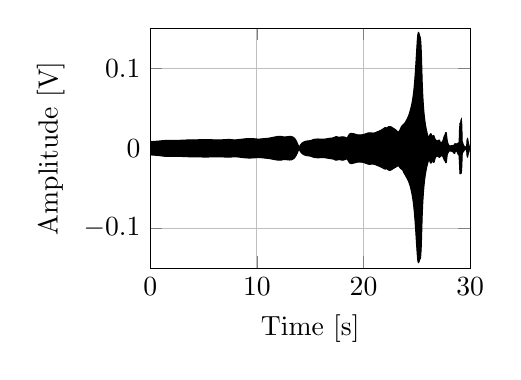
\begin{tikzpicture}

\begin{axis}[%
width=1.6in,
height=1.2in,
at={(0.758in,0.481in)},
scale only axis,
xmin=0,
xmax=30,
xmajorgrids,
ymin=-0.15,
ymax=0.15,
ymajorgrids,
xlabel={Time [s]},
ylabel={Amplitude [V]},
axis background/.style={fill=white}
]
\addplot[fill=black,draw=black,forget plot] plot table[row sep=crcr]{%
2.08333333333333e-05	0.0113942623138428\\
0.0417454218822439	0.00829088687896729\\
0.0834700104311544	0.00816190242767334\\
0.125194598980065	0.0081932544708252\\
0.166919187528975	0.00823116302490234\\
0.208643776077886	0.0082695484161377\\
0.250368364626797	0.0083087682723999\\
0.292092953175707	0.00837302207946777\\
0.333817541724618	0.00839591026306152\\
0.375542130273528	0.00844228267669678\\
0.417266718822439	0.00849699974060059\\
0.458991307371349	0.00854277610778809\\
0.50071589592026	0.00860750675201416\\
0.54244048446917	0.00862538814544678\\
0.584165073018081	0.00868391990661621\\
0.625889661566991	0.00874102115631104\\
0.667614250115902	0.00878274440765381\\
0.709338838664812	0.00881493091583252\\
0.751063427213723	0.00886297225952148\\
0.792788015762633	0.00893044471740723\\
0.834512604311544	0.00897431373596191\\
0.876237192860454	0.00901150703430176\\
0.917961781409365	0.00908493995666504\\
0.959686369958275	0.00915277004241943\\
1.00141095850719	0.0092017650604248\\
1.0431355470561	0.00923347473144531\\
1.08486013560501	0.00929343700408936\\
1.12658472415392	0.00933098793029785\\
1.16830931270283	0.00938868522644043\\
1.21003390125174	0.00944077968597412\\
1.25175848980065	0.0094829797744751\\
1.29348307834956	0.00954926013946533\\
1.33520766689847	0.00959503650665283\\
1.37693225544738	0.00963771343231201\\
1.41865684399629	0.00967609882354736\\
1.4603814325452	0.00971567630767822\\
1.50210602109411	0.00974941253662109\\
1.54383060964302	0.00976872444152832\\
1.58555519819193	0.00978279113769531\\
1.62727978674084	0.00978291034698486\\
1.66900437528975	0.00977420806884766\\
1.71072896383866	0.00976836681365967\\
1.75245355238758	0.00977170467376709\\
1.79417814093649	0.00975668430328369\\
1.8359027294854	0.00974941253662109\\
1.87762731803431	0.00973665714263916\\
1.91935190658322	0.00972485542297363\\
1.96107649513213	0.00970852375030518\\
2.00280108368104	0.00970816612243652\\
2.04452567222995	0.00969779491424561\\
2.08625026077886	0.00969827175140381\\
2.12797484932777	0.0097048282623291\\
2.16969943787668	0.00969910621643066\\
2.21142402642559	0.00969326496124268\\
2.2531486149745	0.00970697402954102\\
2.29487320352341	0.00971686840057373\\
2.33659779207232	0.00972414016723633\\
2.37832238062123	0.00973188877105713\\
2.42004696917014	0.00972354412078857\\
2.46177155771905	0.00974404811859131\\
2.50349614626796	0.00977444648742676\\
2.54522073481687	0.00977790355682373\\
2.58694532336579	0.00980913639068604\\
2.6286699119147	0.00980925559997559\\
2.67039450046361	0.0098186731338501\\
2.71211908901252	0.00983035564422607\\
2.75384367756143	0.00985264778137207\\
2.79556826611034	0.00986766815185547\\
2.83729285465925	0.00989878177642822\\
2.87901744320816	0.00991344451904297\\
2.92074203175707	0.00992631912231445\\
2.96246662030598	0.00996601581573486\\
3.00419120885489	0.00999116897583008\\
3.0459157974038	0.0100135803222656\\
3.08764038595271	0.0100528001785278\\
3.12936497450162	0.0100795030593872\\
3.17108956305053	0.0100895166397095\\
3.21281415159944	0.0101282596588135\\
3.25453874014835	0.0101447105407715\\
3.29626332869726	0.0101814270019531\\
3.33798791724618	0.0101956129074097\\
3.37971250579509	0.0102150440216064\\
3.421437094344	0.0102406740188599\\
3.46316168289291	0.0102685689926147\\
3.50488627144182	0.0102959871292114\\
3.54661085999073	0.0103257894515991\\
3.58833544853964	0.0103374719619751\\
3.63006003708855	0.0103477239608765\\
3.67178462563746	0.0103528499603271\\
3.71350921418637	0.0103640556335449\\
3.75523380273528	0.0103760957717896\\
3.79695839128419	0.0104002952575684\\
3.8386829798331	0.0103920698165894\\
3.88040756838201	0.0104008913040161\\
3.92213215693092	0.0103983879089355\\
3.96385674547983	0.0104092359542847\\
4.00558133402874	0.0104225873947144\\
4.04730592257765	0.0104175806045532\\
4.08903051112656	0.0104261636734009\\
4.13075509967547	0.0104316473007202\\
4.17247968822439	0.0104416608810425\\
4.2142042767733	0.0104471445083618\\
4.25592886532221	0.0104612112045288\\
4.29765345387112	0.0104759931564331\\
4.33937804242003	0.0104820728302002\\
4.38110263096894	0.0104959011077881\\
4.42282721951785	0.0105243921279907\\
4.46455180806676	0.0105077028274536\\
4.50627639661567	0.0105410814285278\\
4.54800098516458	0.0105702877044678\\
4.58972557371349	0.0105710029602051\\
4.6314501622624	0.0105856657028198\\
4.67317475081131	0.010593056678772\\
4.71489933936022	0.0106030702590942\\
4.75662392790913	0.010624885559082\\
4.79834851645804	0.0106714963912964\\
4.84007310500695	0.0106507539749146\\
4.88179769355586	0.0106732845306396\\
4.92352228210478	0.010692834854126\\
4.96524687065368	0.0106824636459351\\
5.0069714592026	0.0107008218765259\\
5.04869604775151	0.0107036828994751\\
5.09042063630042	0.0107138156890869\\
5.13214522484933	0.0107250213623047\\
5.17386981339824	0.0107383728027344\\
5.21559440194715	0.010736346244812\\
5.25731899049606	0.0107240676879883\\
5.29904357904497	0.0107258558273315\\
5.34076816759388	0.0107271671295166\\
5.38249275614279	0.0107125043869019\\
5.4242173446917	0.0107312202453613\\
5.46594193324061	0.0107096433639526\\
5.50766652178952	0.010688304901123\\
5.54939111033843	0.0106769800186157\\
5.59111569888734	0.0106531381607056\\
5.63284028743625	0.0106439590454102\\
5.67456487598516	0.0106256008148193\\
5.71628946453407	0.0106052160263062\\
5.75801405308299	0.0105521678924561\\
5.7997386416319	0.0105510950088501\\
5.84146323018081	0.0105135440826416\\
5.88318781872972	0.0104985237121582\\
5.92491240727863	0.010492205619812\\
5.96663699582754	0.0104633569717407\\
6.00836158437645	0.0104550123214722\\
6.05008617292536	0.0104275941848755\\
6.09181076147427	0.010413646697998\\
6.13353535002318	0.0103986263275146\\
6.17525993857209	0.0103857517242432\\
6.216984527121	0.0103919506072998\\
6.25870911566991	0.0104111433029175\\
6.30043370421882	0.0103940963745117\\
6.34215829276773	0.0104020833969116\\
6.38388288131664	0.010401725769043\\
6.42560746986555	0.0104111433029175\\
6.46733205841446	0.0104062557220459\\
6.50905664696338	0.0104279518127441\\
6.55078123551229	0.0104237794876099\\
6.5925058240612	0.010440468788147\\
6.63423041261011	0.010461688041687\\
6.67595500115902	0.010461688041687\\
6.71767958970793	0.0104776620864868\\
6.75940417825684	0.0105034112930298\\
6.80112876680575	0.0105279684066772\\
6.84285335535466	0.0105477571487427\\
6.88457794390357	0.0105776786804199\\
6.92630253245248	0.0105881690979004\\
6.96802712100139	0.0106377601623535\\
7.0097517095503	0.0106774568557739\\
7.05147629809921	0.0107012987136841\\
7.09320088664812	0.0107371807098389\\
7.13492547519703	0.010794997215271\\
7.17665006374594	0.0108188390731812\\
7.21837465229485	0.010838508605957\\
7.26009924084376	0.010880708694458\\
7.30182382939268	0.0108869075775146\\
7.34354841794159	0.0108964443206787\\
7.3852730064905	0.0109134912490845\\
7.42699759503941	0.0109093189239502\\
7.46872218358832	0.0108965635299683\\
7.51044677213723	0.0108630657196045\\
7.55217136068614	0.010802149772644\\
7.59389594923505	0.0107488632202148\\
7.63562053778396	0.0106890201568604\\
7.67734512633287	0.0106164216995239\\
7.71906971488178	0.0105421543121338\\
7.76079430343069	0.0104725360870361\\
7.8025188919796	0.0104317665100098\\
7.84424348052851	0.0103904008865356\\
7.88596806907742	0.0103800296783447\\
7.92769265762633	0.0103586912155151\\
7.96941724617524	0.0103760957717896\\
8.01114183472416	0.0104219913482666\\
8.05286642327307	0.0104528665542603\\
8.09459101182198	0.0105187892913818\\
8.13631560037089	0.0105619430541992\\
8.1780401889198	0.0106202363967896\\
8.21976477746871	0.0106871128082275\\
8.26148936601762	0.0107446908950806\\
8.30321395456653	0.0108059644699097\\
8.34493854311544	0.010887622833252\\
8.38666313166435	0.0109357833862305\\
8.42838772021326	0.0109992027282715\\
8.47011230876217	0.0110762119293213\\
8.51183689731108	0.0111377239227295\\
8.55356148585999	0.0111801624298096\\
8.5952860744089	0.0112690925598145\\
8.63701066295781	0.0113228559494019\\
8.67873525150672	0.0113829374313354\\
8.72045984005563	0.0114455223083496\\
8.76218442860454	0.0115017890930176\\
8.80390901715345	0.0115691423416138\\
8.84563360570237	0.0116307735443115\\
8.88735819425128	0.0116676092147827\\
8.92908278280018	0.0117268562316895\\
8.9708073713491	0.0118035078048706\\
9.01253195989801	0.0118147134780884\\
9.05425654844692	0.0118619203567505\\
9.09598113699583	0.0118932723999023\\
9.13770572554474	0.0119321346282959\\
9.17943031409365	0.0119595527648926\\
9.22115490264256	0.0119895935058594\\
9.26287949119147	0.0119942426681519\\
9.30460407974038	0.0119855403900146\\
9.34632866828929	0.011993408203125\\
9.3880532568382	0.0119847059249878\\
9.42977784538711	0.0119955539703369\\
9.47150243393602	0.0119667053222656\\
9.51322702248493	0.0119537115097046\\
9.55495161103384	0.0119032859802246\\
9.59667619958275	0.0118762254714966\\
9.63840078813166	0.0118461847305298\\
9.68012537668058	0.0118163824081421\\
9.72184996522949	0.0117794275283813\\
9.7635745537784	0.0117802619934082\\
9.80529914232731	0.0117013454437256\\
9.84702373087622	0.0116596221923828\\
9.88874831942513	0.011614203453064\\
9.93047290797404	0.0115708112716675\\
9.97219749652295	0.0115410089492798\\
10.0139220850719	0.0114614963531494\\
10.0556466736208	0.0114158391952515\\
10.0973712621697	0.0113879442214966\\
10.1390958507186	0.0113658905029297\\
10.1808204392675	0.0113563537597656\\
10.2225450278164	0.0113716125488281\\
10.2642696163653	0.0113954544067383\\
10.3059942049142	0.0114538669586182\\
10.3477187934631	0.0114964246749878\\
10.3894433820121	0.0115419626235962\\
10.431167970561	0.0116304159164429\\
10.4728925591099	0.0116804838180542\\
10.5146171476588	0.0117305517196655\\
10.5563417362077	0.0118038654327393\\
10.5980663247566	0.0118789672851563\\
10.6397909133055	0.0119270086288452\\
10.6815155018544	0.0119820833206177\\
10.7232400904033	0.0120391845703125\\
10.7649646789523	0.012076735496521\\
10.8066892675012	0.0121059417724609\\
10.8484138560501	0.0121577978134155\\
10.890138444599	0.0121808052062988\\
10.9318630331479	0.0122424364089966\\
10.9735876216968	0.0122891664505005\\
11.0153122102457	0.0123604536056519\\
11.0570367987946	0.0124201774597168\\
11.0987613873435	0.012507438659668\\
11.1404859758924	0.0126070976257324\\
11.1822105644414	0.0126873254776001\\
11.2239351529903	0.0127902030944824\\
11.2656597415392	0.0128899812698364\\
11.3073843300881	0.0130234956741333\\
11.349108918637	0.0131070613861084\\
11.3908335071859	0.0132313966751099\\
11.4325580957348	0.0133460760116577\\
11.4742826842837	0.0134791135787964\\
11.5160072728326	0.0135729312896729\\
11.5577318613816	0.0136982202529907\\
11.5994564499305	0.0138028860092163\\
11.6411810384794	0.0139143466949463\\
11.6829056270283	0.0140161514282227\\
11.7246302155772	0.0141229629516602\\
11.7663548041261	0.0142431259155273\\
11.808079392675	0.0143195390701294\\
11.8498039812239	0.0144040584564209\\
11.8915285697728	0.0144946575164795\\
11.9332531583217	0.0145910978317261\\
11.9749777468707	0.0146702527999878\\
12.0167023354196	0.0147042274475098\\
12.0584269239685	0.0147408246994019\\
12.1001515125174	0.0147584676742554\\
12.1418761010663	0.0147675275802612\\
12.1836006896152	0.0147678852081299\\
12.2253252781641	0.014737606048584\\
12.267049866713	0.0146942138671875\\
12.3087744552619	0.0145617723464966\\
12.3504990438108	0.01447594165802\\
12.3922236323598	0.0143582820892334\\
12.4339482209087	0.0142744779586792\\
12.4756728094576	0.014165997505188\\
12.5173973980065	0.0140732526779175\\
12.5591219865554	0.0140211582183838\\
12.6008465751043	0.0140103101730347\\
12.6425711636532	0.0140440464019775\\
12.6842957522021	0.0140941143035889\\
12.726020340751	0.0141386985778809\\
12.7677449293	0.0142180919647217\\
12.8094695178489	0.0143122673034668\\
12.8511941063978	0.0144103765487671\\
12.8929186949467	0.0144859552383423\\
12.9346432834956	0.0145372152328491\\
12.9763678720445	0.0146024227142334\\
13.0180924605934	0.0146586894989014\\
13.0598170491423	0.0146702527999878\\
13.1015416376912	0.014670729637146\\
13.1432662262401	0.0146702527999878\\
13.1849908147891	0.0146102905273438\\
13.226715403338	0.0145364999771118\\
13.2684399918869	0.0143954753875732\\
13.3101645804358	0.0141972303390503\\
13.3518891689847	0.013979434967041\\
13.3936137575336	0.0136640071868896\\
13.4353383460825	0.0133869647979736\\
13.4770629346314	0.0129083395004272\\
13.5187875231803	0.012401819229126\\
13.5605121117293	0.0117309093475342\\
13.6022367002782	0.0109891891479492\\
13.6439612888271	0.0101124048233032\\
13.685685877376	0.00915110111236572\\
13.7274104659249	0.00805604457855225\\
13.7691350544738	0.00685441493988037\\
13.8108596430227	0.00552380084991455\\
13.8525842315716	0.00418686866760254\\
13.8943088201205	0.00289440155029297\\
13.9360334086694	0.00178420543670654\\
13.9777579972184	0.00165677070617676\\
14.0194825857673	0.00262069702148438\\
14.0612071743162	0.00353264808654785\\
14.1029317628651	0.00436758995056152\\
14.144656351414	0.00509977340698242\\
14.1863809399629	0.00571370124816895\\
14.2281055285118	0.00626468658447266\\
14.2698301170607	0.00674343109130859\\
14.3115547056096	0.00712299346923828\\
14.3532792941586	0.00745129585266113\\
14.3950038827075	0.0077441930770874\\
14.4367284712564	0.00802004337310791\\
14.4784530598053	0.00824117660522461\\
14.5201776483542	0.0084235668182373\\
14.5619022369031	0.00858414173126221\\
14.603626825452	0.00872063636779785\\
14.6453514140009	0.00883567333221436\\
14.6870760025498	0.00891876220703125\\
14.7288005910988	0.00899887084960938\\
14.7705251796477	0.00906312465667725\\
14.8122497681966	0.00912952423095703\\
14.8539743567455	0.00921130180358887\\
14.8956989452944	0.00926709175109863\\
14.9374235338433	0.0093311071395874\\
14.9791481223922	0.00942158699035645\\
15.0208727109411	0.00956058502197266\\
15.06259729949	0.00968480110168457\\
15.1043218880389	0.00985932350158691\\
15.1460464765879	0.0100594758987427\\
15.1877710651368	0.01025390625\\
15.2294956536857	0.0104728937149048\\
15.2712202422346	0.0106781721115112\\
15.3129448307835	0.0108400583267212\\
15.3546694193324	0.010985255241394\\
15.3963940078813	0.0111068487167358\\
15.4381185964302	0.0112005472183228\\
15.4798431849791	0.0112849473953247\\
15.521567773528	0.0113582611083984\\
15.563292362077	0.0113930702209473\\
15.6050169506259	0.0114071369171143\\
15.6467415391748	0.0114408731460571\\
15.6884661277237	0.0114706754684448\\
15.7301907162726	0.0114651918411255\\
15.7719153048215	0.0114750862121582\\
15.8136398933704	0.0114505290985107\\
15.8553644819193	0.0114434957504272\\
15.8970890704682	0.0114383697509766\\
15.9388136590172	0.0114046335220337\\
15.9805382475661	0.0113633871078491\\
16.022262836115	0.0113532543182373\\
16.0639874246639	0.0113248825073242\\
16.1057120132128	0.011273980140686\\
16.1474366017617	0.0112365484237671\\
16.1891611903106	0.0112427473068237\\
16.2308857788595	0.0112248659133911\\
16.2726103674084	0.0112439393997192\\
16.3143349559573	0.0112924575805664\\
16.3560595445063	0.0113638639450073\\
16.3977841330552	0.0114331245422363\\
16.4395087216041	0.0115131139755249\\
16.481233310153	0.0116007328033447\\
16.5229578987019	0.0117172002792358\\
16.5646824872508	0.0118080377578735\\
16.6064070757997	0.0118964910507202\\
16.6481316643486	0.0120166540145874\\
16.6898562528975	0.0120859146118164\\
16.7315808414465	0.0121544599533081\\
16.7733054299954	0.012226939201355\\
16.8150300185443	0.0123187303543091\\
16.8567546070932	0.0124144554138184\\
16.8984791956421	0.0124548673629761\\
16.940203784191	0.0125182867050171\\
16.9819283727399	0.0125758647918701\\
17.0236529612888	0.0126584768295288\\
17.0653775498377	0.0127372741699219\\
17.1071021383867	0.0128670930862427\\
17.1488267269356	0.0129997730255127\\
17.1905513154845	0.0131481885910034\\
17.2322759040334	0.0133693218231201\\
17.2740004925823	0.0136631727218628\\
17.3157250811312	0.013934850692749\\
17.3574496696801	0.0142035484313965\\
17.399174258229	0.0143387317657471\\
17.4408988467779	0.0143603086471558\\
17.4826234353268	0.0143387317657471\\
17.5243480238758	0.0142385959625244\\
17.5660726124247	0.0140465497970581\\
17.6077972009736	0.0138800144195557\\
17.6495217895225	0.0137039422988892\\
17.6912463780714	0.0136256217956543\\
17.7329709666203	0.0136539936065674\\
17.7746955551692	0.0137131214141846\\
17.8164201437181	0.0138174295425415\\
17.858144732267	0.0139714479446411\\
17.8998693208159	0.0140658617019653\\
17.9415939093649	0.0141353607177734\\
17.9833184979138	0.0142005681991577\\
18.0250430864627	0.0142451524734497\\
18.0667676750116	0.0142556428909302\\
18.1084922635605	0.0142221450805664\\
18.1502168521094	0.0141061544418335\\
18.1919414406583	0.013946533203125\\
18.2336660292072	0.013741135597229\\
18.2753906177561	0.0135041475296021\\
18.3171152063051	0.013230562210083\\
18.358839794854	0.0129725933074951\\
18.4005643834029	0.0127698183059692\\
18.4422889719518	0.0128542184829712\\
18.4840135605007	0.0133035182952881\\
18.5257381490496	0.0141111612319946\\
18.5674627375985	0.0151150226593018\\
18.6091873261474	0.0161937475204468\\
18.6509119146963	0.0170919895172119\\
18.6926365032453	0.0177032947540283\\
18.7343610917942	0.0181496143341064\\
18.7760856803431	0.0183612108230591\\
18.817810268892	0.0184909105300903\\
18.8595348574409	0.0184900760650635\\
18.9012594459898	0.0184675455093384\\
18.9429840345387	0.0183607339859009\\
18.9847086230876	0.018251895904541\\
19.0264332116365	0.0181654691696167\\
19.0681578001854	0.0180470943450928\\
19.1098823887344	0.0179555416107178\\
19.1516069772833	0.0177874565124512\\
19.1933315658322	0.0176022052764893\\
19.2350561543811	0.0174229145050049\\
19.27678074293	0.0172655582427979\\
19.3185053314789	0.0171111822128296\\
19.3602299200278	0.0169497728347778\\
19.4019545085767	0.0168157815933228\\
19.4436790971256	0.016693115234375\\
19.4854036856745	0.0166218280792236\\
19.5271282742235	0.0165559053421021\\
19.5688528627724	0.0165392160415649\\
19.6105774513213	0.0165283679962158\\
19.6523020398702	0.0165469646453857\\
19.6940266284191	0.0165870189666748\\
19.735751216968	0.0166168212890625\\
19.7774758055169	0.0166709423065186\\
19.8192003940658	0.0167360305786133\\
19.8609249826147	0.0168262720108032\\
19.9026495711637	0.0169438123703003\\
19.9443741597126	0.0170327425003052\\
19.9860987482615	0.0171369314193726\\
20.0278233368104	0.0172576904296875\\
20.0695479253593	0.0174340009689331\\
20.1112725139082	0.0175614356994629\\
20.1529971024571	0.0177373886108398\\
20.194721691006	0.0179321765899658\\
20.2364462795549	0.0181537866592407\\
20.2781708681038	0.0183658599853516\\
20.3198954566528	0.0185823440551758\\
20.3616200452017	0.0187830924987793\\
20.4033446337506	0.0189470052719116\\
20.4450692222995	0.0190809965133667\\
20.4867938108484	0.0191706418991089\\
20.5285183993973	0.0192203521728516\\
20.5702429879462	0.019231915473938\\
20.6119675764951	0.0192281007766724\\
20.653692165044	0.0191776752471924\\
20.695416753593	0.0191197395324707\\
20.7371413421419	0.0190595388412476\\
20.7788659306908	0.0190016031265259\\
20.8205905192397	0.0189636945724487\\
20.8623151077886	0.0189056396484375\\
20.9040396963375	0.018895149230957\\
20.9457642848864	0.0189398527145386\\
20.9874888734353	0.0189944505691528\\
21.0292134619842	0.0191519260406494\\
21.0709380505331	0.0193146467208862\\
21.1126626390821	0.0194823741912842\\
21.154387227631	0.019695520401001\\
21.1961118161799	0.0199525356292725\\
21.2378364047288	0.020194411277771\\
21.2795609932777	0.020445704460144\\
21.3212855818266	0.0206722021102905\\
21.3630101703755	0.0209243297576904\\
21.4047347589244	0.0211095809936523\\
21.4464593474733	0.0213415622711182\\
21.4881839360223	0.0216009616851807\\
21.5299085245712	0.0218217372894287\\
21.5716331131201	0.0220507383346558\\
21.613357701669	0.0223489999771118\\
21.6550822902179	0.0226349830627441\\
21.6968068787668	0.0229681730270386\\
21.7385314673157	0.0232745409011841\\
21.7802560558646	0.0236674547195435\\
21.8219806444135	0.0240671634674072\\
21.8637052329624	0.0244702100753784\\
21.9054298215114	0.0248830318450928\\
21.9471544100603	0.0252479314804077\\
21.9888789986092	0.0255330801010132\\
22.0306035871581	0.025623083114624\\
22.072328175707	0.0256264209747314\\
22.1140527642559	0.0255446434020996\\
22.1557773528048	0.02543044090271\\
22.1975019413537	0.0255500078201294\\
22.2392265299026	0.0258854627609253\\
22.2809511184516	0.0262682437896729\\
22.3226757070005	0.0265686511993408\\
22.3644002955494	0.0268886089324951\\
22.4061248840983	0.0269861221313477\\
22.4478494726472	0.0270559787750244\\
22.4895740611961	0.0270254611968994\\
22.531298649745	0.0269443988800049\\
22.5730232382939	0.0267041921615601\\
22.6147478268428	0.0264041423797607\\
22.6564724153917	0.0261270999908447\\
22.6981970039407	0.0256744623184204\\
22.7399215924896	0.025294303894043\\
22.7816461810385	0.0249384641647339\\
22.8233707695874	0.024603009223938\\
22.8650953581363	0.0242496728897095\\
22.9068199466852	0.0239053964614868\\
22.9485445352341	0.0234622955322266\\
22.990269123783	0.0230779647827148\\
23.0319937123319	0.0226974487304688\\
23.0737183008809	0.0221329927444458\\
23.1154428894298	0.0215408802032471\\
23.1571674779787	0.021124005317688\\
23.1988920665276	0.0208607912063599\\
23.2406166550765	0.0201030969619751\\
23.2823412436254	0.0202142000198364\\
23.3240658321743	0.0207192897796631\\
23.3657904207232	0.0215063095092773\\
23.4075150092721	0.0226578712463379\\
23.449239597821	0.0240292549133301\\
23.49096418637	0.0253231525421143\\
23.5326887749189	0.0264760255813599\\
23.5744133634678	0.0273241996765137\\
23.6161379520167	0.0281366109848022\\
23.6578625405656	0.0287598371505737\\
23.6995871291145	0.0293393135070801\\
23.7413117176634	0.0297406911849976\\
23.7830363062123	0.030133843421936\\
23.8247608947612	0.0307341814041138\\
23.8664854833102	0.0314919948577881\\
23.9082100718591	0.0322674512863159\\
23.949934660408	0.0331833362579346\\
23.9916592489569	0.0341380834579468\\
24.0333838375058	0.0350855588912964\\
24.0751084260547	0.0361357927322388\\
24.1168330146036	0.0372881889343262\\
24.1585576031525	0.0385874509811401\\
24.2002821917014	0.0399467945098877\\
24.2420067802503	0.0413480997085571\\
24.2837313687993	0.0429809093475342\\
24.3254559573482	0.044714093208313\\
24.3671805458971	0.0465803146362305\\
24.408905134446	0.0485935211181641\\
24.4506297229949	0.050800085067749\\
24.4923543115438	0.0532447099685669\\
24.5340789000927	0.0558316707611084\\
24.5758034886416	0.0589557886123657\\
24.6175280771905	0.0623215436935425\\
24.6592526657395	0.0661643743515015\\
24.7009772542884	0.0706945657730103\\
24.7427018428373	0.0760377645492554\\
24.7844264313862	0.0823279619216919\\
24.8261510199351	0.0898284912109375\\
24.867875608484	0.0976375341415405\\
24.9096001970329	0.106538653373718\\
24.9513247855818	0.11583423614502\\
24.9930493741307	0.125002503395081\\
25.0347739626796	0.133956789970398\\
25.0764985512286	0.140738725662231\\
25.1182231397775	0.144140005111694\\
25.1599477283264	0.144588112831116\\
25.2016723168753	0.143488883972168\\
25.2433969054242	0.140970706939697\\
25.2851214939731	0.139572739601135\\
25.326846082522	0.137726068496704\\
25.3685706710709	0.132014870643616\\
25.4102952596198	0.120246887207031\\
25.4520198481687	0.102569460868835\\
25.4937444367177	0.0830684900283813\\
25.5354690252666	0.0695452690124512\\
25.5771936138155	0.059396505355835\\
25.6189182023644	0.05119788646698\\
25.6606427909133	0.0444579124450684\\
25.7023673794622	0.039044976234436\\
25.7440919680111	0.0344971418380737\\
25.78581655656	0.0307368040084839\\
25.8275411451089	0.0272449254989624\\
25.8692657336579	0.0242825746536255\\
25.9109903222068	0.0215767621994019\\
25.9527149107557	0.0191923379898071\\
25.9944394993046	0.0170477628707886\\
26.0361640878535	0.0153229236602783\\
26.0778886764024	0.0142227411270142\\
26.1196132649513	0.0136210918426514\\
26.1613378535002	0.0143477916717529\\
26.2030624420491	0.0159620046615601\\
26.2447870305981	0.01756751537323\\
26.286511619147	0.0179845094680786\\
26.3282362076959	0.0178604125976563\\
26.3699607962448	0.0162191390991211\\
26.4116853847937	0.0141971111297607\\
26.4534099733426	0.0141793489456177\\
26.4951345618915	0.0153818130493164\\
26.5368591504404	0.0158649682998657\\
26.5785837389893	0.0157814025878906\\
26.6203083275383	0.0144866704940796\\
26.6620329160872	0.0126464366912842\\
26.7037575046361	0.0115031003952026\\
26.745482093185	0.0103886127471924\\
26.7872066817339	0.00970065593719482\\
26.8289312702828	0.00980162620544434\\
26.8706558588317	0.00971150398254395\\
26.9123804473806	0.00917458534240723\\
26.9541050359295	0.00880122184753418\\
26.9958296244784	0.00951218605041504\\
27.0375542130274	0.0100506544113159\\
27.0792788015763	0.0101230144500732\\
27.1210033901252	0.00972282886505127\\
27.1627279786741	0.00818705558776855\\
27.204452567223	0.00739634037017822\\
27.2461771557719	0.006866455078125\\
27.2879017443208	0.00695109367370605\\
27.3296263328697	0.00729167461395264\\
27.3713509214186	0.00784850120544434\\
27.4130755099675	0.00871932506561279\\
27.4548000985165	0.00997698307037354\\
27.4965246870654	0.0117588043212891\\
27.5382492756143	0.0139259099960327\\
27.5799738641632	0.015549898147583\\
27.6216984527121	0.0162312984466553\\
27.663423041261	0.0177611112594604\\
27.7051476298099	0.0194618701934814\\
27.7468722183588	0.0194063186645508\\
27.7885968069077	0.0154396295547485\\
27.8303213954567	0.0102689266204834\\
27.8720459840056	0.00755560398101807\\
27.9137705725545	0.00581622123718262\\
27.9554951611034	0.00451278686523438\\
27.9972197496523	0.00375807285308838\\
28.0389443382012	0.00320529937744141\\
28.0806689267501	0.00275969505310059\\
28.122393515299	0.00241363048553467\\
28.1641181038479	0.0027158260345459\\
28.2058426923968	0.00318050384521484\\
28.2475672809458	0.00320196151733398\\
28.2892918694947	0.00279474258422852\\
28.3310164580436	0.00308680534362793\\
28.3727410465925	0.00342011451721191\\
28.4144656351414	0.00355446338653564\\
28.4561902236903	0.00355076789855957\\
28.4979148122392	0.00419580936431885\\
28.5396394007881	0.00534594058990479\\
28.581363989337	0.00555634498596191\\
28.623088577886	0.00541985034942627\\
28.6648131664349	0.00536608695983887\\
28.7065377549838	0.00527334213256836\\
28.7482623435327	0.00535309314727783\\
28.7899869320816	0.00570452213287354\\
28.8317115206305	0.00616669654846191\\
28.8734361091794	0.00646460056304932\\
28.9151606977283	0.00617516040802002\\
28.9568852862772	0.00557184219360352\\
28.9986098748261	0.0226660966873169\\
29.0403344633751	0.0317338705062866\\
29.082059051924	0.0263825654983521\\
29.1237836404729	0.0349920988082886\\
29.1655082290218	0.0360742807388306\\
29.2072328175707	0.0289243459701538\\
29.2489574061196	0.00723528861999512\\
29.2906819946685	0.00694477558135986\\
29.3324065832174	0.00507152080535889\\
29.3741311717663	0.00346815586090088\\
29.4158557603153	0.00267577171325684\\
29.4575803488642	0.00242531299591064\\
29.4993049374131	0.0017932653427124\\
29.541029525962	0.00149738788604736\\
29.5827541145109	0.00133943557739258\\
29.6244787030598	0.00158345699310303\\
29.6662032916087	0.00274419784545898\\
29.7079278801576	0.0111613273620605\\
29.7496524687065	0.0119098424911499\\
29.7913770572554	0.00936651229858398\\
29.8331016458044	0.0059126615524292\\
29.8748262343533	0.00409436225891113\\
29.9165508229022	0.00181043148040771\\
29.9582754114511	0.000862360000610352\\
30	0.000552892684936523\\
}
\closedcycle;
\addplot[fill=black,draw=black,forget plot] plot table[row sep=crcr]{%
2.08333333333333e-05	-0.0103787183761597\\
0.0417454218822439	-0.00837349891662598\\
0.0834700104311544	-0.00834286212921143\\
0.125194598980065	-0.00836169719696045\\
0.166919187528975	-0.0083993673324585\\
0.208643776077886	-0.00843346118927002\\
0.250368364626797	-0.00846099853515625\\
0.292092953175707	-0.00849020481109619\\
0.333817541724618	-0.00857985019683838\\
0.375542130273528	-0.00860464572906494\\
0.417266718822439	-0.00866472721099854\\
0.458991307371349	-0.00871098041534424\\
0.50071589592026	-0.0087592601776123\\
0.54244048446917	-0.0088118314743042\\
0.584165073018081	-0.00887250900268555\\
0.625889661566991	-0.00891494750976563\\
0.667614250115902	-0.00896966457366943\\
0.709338838664812	-0.00903630256652832\\
0.751063427213723	-0.00908267498016357\\
0.792788015762633	-0.00913619995117188\\
0.834512604311544	-0.00919365882873535\\
0.876237192860454	-0.00925219058990479\\
0.917961781409365	-0.00931930541992188\\
0.959686369958275	-0.00936555862426758\\
1.00141095850719	-0.0094444751739502\\
1.0431355470561	-0.00950539112091064\\
1.08486013560501	-0.00960206985473633\\
1.12658472415392	-0.00966596603393555\\
1.16830931270283	-0.00974774360656738\\
1.21003390125174	-0.00981795787811279\\
1.25175848980065	-0.00985968112945557\\
1.29348307834956	-0.00991082191467285\\
1.33520766689847	-0.00997138023376465\\
1.37693225544738	-0.0100094079971313\\
1.41865684399629	-0.0100619792938232\\
1.4603814325452	-0.0100793838500977\\
1.50210602109411	-0.010103702545166\\
1.54383060964302	-0.0101082324981689\\
1.58555519819193	-0.0100898742675781\\
1.62727978674084	-0.0100990533828735\\
1.66900437528975	-0.0100936889648438\\
1.71072896383866	-0.0100778341293335\\
1.75245355238758	-0.0100444555282593\\
1.79417814093649	-0.0100318193435669\\
1.8359027294854	-0.0100182294845581\\
1.87762731803431	-0.0100201368331909\\
1.91935190658322	-0.00999140739440918\\
1.96107649513213	-0.00998008251190186\\
2.00280108368104	-0.00997722148895264\\
2.04452567222995	-0.00996315479278564\\
2.08625026077886	-0.00997984409332275\\
2.12797484932777	-0.00999057292938232\\
2.16969943787668	-0.0099947452545166\\
2.21142402642559	-0.00998520851135254\\
2.2531486149745	-0.00997352600097656\\
2.29487320352341	-0.00999104976654053\\
2.33659779207232	-0.00998234748840332\\
2.37832238062123	-0.0100076198577881\\
2.42004696917014	-0.010033130645752\\
2.46177155771905	-0.0100289583206177\\
2.50349614626796	-0.0100432634353638\\
2.54522073481687	-0.0100464820861816\\
2.58694532336579	-0.0100619792938232\\
2.6286699119147	-0.0100857019424438\\
2.67039450046361	-0.0100898742675781\\
2.71211908901252	-0.0100966691970825\\
2.75384367756143	-0.010141134262085\\
2.79556826611034	-0.010157585144043\\
2.83729285465925	-0.0101759433746338\\
2.87901744320816	-0.0101937055587769\\
2.92074203175707	-0.0102237462997437\\
2.96246662030598	-0.010226845741272\\
3.00419120885489	-0.010280966758728\\
3.0459157974038	-0.0102969408035278\\
3.08764038595271	-0.0103268623352051\\
3.12936497450162	-0.0103482007980347\\
3.17108956305053	-0.0103994607925415\\
3.21281415159944	-0.010434627532959\\
3.25453874014835	-0.0104511976242065\\
3.29626332869726	-0.0104449987411499\\
3.33798791724618	-0.0104972124099731\\
3.37971250579509	-0.0105212926864624\\
3.421437094344	-0.0105592012405396\\
3.46316168289291	-0.0105700492858887\\
3.50488627144182	-0.0105806589126587\\
3.54661085999073	-0.0105913877487183\\
3.58833544853964	-0.0106239318847656\\
3.63006003708855	-0.0106260776519775\\
3.67178462563746	-0.0106449127197266\\
3.71350921418637	-0.0106489658355713\\
3.75523380273528	-0.0106468200683594\\
3.79695839128419	-0.0106360912322998\\
3.8386829798331	-0.0106509923934937\\
3.88040756838201	-0.0106614828109741\\
3.92213215693092	-0.010643482208252\\
3.96385674547983	-0.010648250579834\\
4.00558133402874	-0.010633111000061\\
4.04730592257765	-0.0106352567672729\\
4.08903051112656	-0.0106385946273804\\
4.13075509967547	-0.0106502771377563\\
4.17247968822439	-0.0106624364852905\\
4.2142042767733	-0.0106693506240845\\
4.25592886532221	-0.0106682777404785\\
4.29765345387112	-0.010708212852478\\
4.33937804242003	-0.0107135772705078\\
4.38110263096894	-0.0107036828994751\\
4.42282721951785	-0.0107040405273438\\
4.46455180806676	-0.0107461214065552\\
4.50627639661567	-0.0107470750808716\\
4.54800098516458	-0.0107617378234863\\
4.58972557371349	-0.0107671022415161\\
4.6314501622624	-0.0107816457748413\\
4.67317475081131	-0.0108180046081543\\
4.71489933936022	-0.0108309984207153\\
4.75662392790913	-0.0108238458633423\\
4.79834851645804	-0.0108546018600464\\
4.84007310500695	-0.0108710527420044\\
4.88179769355586	-0.0109114646911621\\
4.92352228210478	-0.0108921527862549\\
4.96524687065368	-0.0109193325042725\\
5.0069714592026	-0.0109119415283203\\
5.04869604775151	-0.0109113454818726\\
5.09042063630042	-0.0109156370162964\\
5.13214522484933	-0.0109306573867798\\
5.17386981339824	-0.0109443664550781\\
5.21559440194715	-0.0109531879425049\\
5.25731899049606	-0.0109544992446899\\
5.29904357904497	-0.0109406709671021\\
5.34076816759388	-0.0109610557556152\\
5.38249275614279	-0.0109411478042603\\
5.4242173446917	-0.0109472274780273\\
5.46594193324061	-0.0109235048294067\\
5.50766652178952	-0.0108946561813354\\
5.54939111033843	-0.0108894109725952\\
5.59111569888734	-0.0108797550201416\\
5.63284028743625	-0.0108476877212524\\
5.67456487598516	-0.0108485221862793\\
5.71628946453407	-0.0108305215835571\\
5.75801405308299	-0.0108013153076172\\
5.7997386416319	-0.0107959508895874\\
5.84146323018081	-0.0107736587524414\\
5.88318781872972	-0.0107450485229492\\
5.92491240727863	-0.0107367038726807\\
5.96663699582754	-0.0107299089431763\\
6.00836158437645	-0.0107173919677734\\
6.05008617292536	-0.0107183456420898\\
6.09181076147427	-0.0106943845748901\\
6.13353535002318	-0.0106960535049438\\
6.17525993857209	-0.0107007026672363\\
6.216984527121	-0.0107043981552124\\
6.25870911566991	-0.0106899738311768\\
6.30043370421882	-0.0106898546218872\\
6.34215829276773	-0.0107090473175049\\
6.38388288131664	-0.0107103586196899\\
6.42560746986555	-0.0107136964797974\\
6.46733205841446	-0.010741114616394\\
6.50905664696338	-0.0107408761978149\\
6.55078123551229	-0.0107636451721191\\
6.5925058240612	-0.0107591152191162\\
6.63423041261011	-0.0107916593551636\\
6.67595500115902	-0.0108159780502319\\
6.71767958970793	-0.0108153820037842\\
6.75940417825684	-0.010831356048584\\
6.80112876680575	-0.0108437538146973\\
6.84285335535466	-0.0108671188354492\\
6.88457794390357	-0.0108896493911743\\
6.92630253245248	-0.0109198093414307\\
6.96802712100139	-0.010915994644165\\
7.0097517095503	-0.0109361410140991\\
7.05147629809921	-0.010958194732666\\
7.09320088664812	-0.0110107660293579\\
7.13492547519703	-0.0110219717025757\\
7.17665006374594	-0.0110571384429932\\
7.21837465229485	-0.011085033416748\\
7.26009924084376	-0.0111037492752075\\
7.30182382939268	-0.0111180543899536\\
7.34354841794159	-0.0111238956451416\\
7.3852730064905	-0.0111376047134399\\
7.42699759503941	-0.0111258029937744\\
7.46872218358832	-0.0111024379730225\\
7.51044677213723	-0.0110470056533813\\
7.55217136068614	-0.0110061168670654\\
7.59389594923505	-0.0109423398971558\\
7.63562053778396	-0.0108659267425537\\
7.67734512633287	-0.0108063220977783\\
7.71906971488178	-0.0107377767562866\\
7.76079430343069	-0.010688304901123\\
7.8025188919796	-0.0105975866317749\\
7.84424348052851	-0.0105972290039063\\
7.88596806907742	-0.0105671882629395\\
7.92769265762633	-0.0105963945388794\\
7.96941724617524	-0.0106050968170166\\
8.01114183472416	-0.0106290578842163\\
8.05286642327307	-0.010673999786377\\
8.09459101182198	-0.0107223987579346\\
8.13631560037089	-0.0107728242874146\\
8.1780401889198	-0.0108479261398315\\
8.21976477746871	-0.0109138488769531\\
8.26148936601762	-0.0109786987304688\\
8.30321395456653	-0.0110461711883545\\
8.34493854311544	-0.011115550994873\\
8.38666313166435	-0.0111597776412964\\
8.42838772021326	-0.0112310647964478\\
8.47011230876217	-0.0112990140914917\\
8.51183689731108	-0.0113542079925537\\
8.55356148585999	-0.0114188194274902\\
8.5952860744089	-0.0114867687225342\\
8.63701066295781	-0.0115418434143066\\
8.67873525150672	-0.011610746383667\\
8.72045984005563	-0.0116612911224365\\
8.76218442860454	-0.0117208957672119\\
8.80390901715345	-0.0117976665496826\\
8.84563360570237	-0.0118532180786133\\
8.88735819425128	-0.011913537979126\\
8.92908278280018	-0.0119458436965942\\
8.9708073713491	-0.0119969844818115\\
9.01253195989801	-0.0120387077331543\\
9.05425654844692	-0.0120925903320313\\
9.09598113699583	-0.0121126174926758\\
9.13770572554474	-0.0121535062789917\\
9.17943031409365	-0.0121880769729614\\
9.22115490264256	-0.0122082233428955\\
9.26287949119147	-0.0122107267379761\\
9.30460407974038	-0.0122170448303223\\
9.34632866828929	-0.0122249126434326\\
9.3880532568382	-0.0122153759002686\\
9.42977784538711	-0.0121947526931763\\
9.47150243393602	-0.0121628046035767\\
9.51322702248493	-0.0121418237686157\\
9.55495161103384	-0.0121322870254517\\
9.59667619958275	-0.0120909214019775\\
9.63840078813166	-0.0120588541030884\\
9.68012537668058	-0.0120179653167725\\
9.72184996522949	-0.0119853019714355\\
9.7635745537784	-0.0119516849517822\\
9.80529914232731	-0.0119185447692871\\
9.84702373087622	-0.0118706226348877\\
9.88874831942513	-0.0118277072906494\\
9.93047290797404	-0.0117614269256592\\
9.97219749652295	-0.0117095708847046\\
10.0139220850719	-0.0116482973098755\\
10.0556466736208	-0.0116144418716431\\
10.0973712621697	-0.0115772485733032\\
10.1390958507186	-0.0115498304367065\\
10.1808204392675	-0.0115597248077393\\
10.2225450278164	-0.0115530490875244\\
10.2642696163653	-0.0116007328033447\\
10.3059942049142	-0.011637806892395\\
10.3477187934631	-0.0116854906082153\\
10.3894433820121	-0.0117517709732056\\
10.431167970561	-0.0118159055709839\\
10.4728925591099	-0.0118573904037476\\
10.5146171476588	-0.0119307041168213\\
10.5563417362077	-0.0120091438293457\\
10.5980663247566	-0.0120730400085449\\
10.6397909133055	-0.0121314525604248\\
10.6815155018544	-0.0121957063674927\\
10.7232400904033	-0.012245774269104\\
10.7649646789523	-0.0123271942138672\\
10.8066892675012	-0.012371301651001\\
10.8484138560501	-0.0123946666717529\\
10.890138444599	-0.0124577283859253\\
10.9318630331479	-0.0124876499176025\\
10.9735876216968	-0.0125406980514526\\
11.0153122102457	-0.0125977993011475\\
11.0570367987946	-0.0126758813858032\\
11.0987613873435	-0.0127643346786499\\
11.1404859758924	-0.0128506422042847\\
11.1822105644414	-0.0129417181015015\\
11.2239351529903	-0.0130423307418823\\
11.2656597415392	-0.0131527185440063\\
11.3073843300881	-0.0132734775543213\\
11.349108918637	-0.0133785009384155\\
11.3908335071859	-0.0134773254394531\\
11.4325580957348	-0.0135771036148071\\
11.4742826842837	-0.0136932134628296\\
11.5160072728326	-0.013803243637085\\
11.5577318613816	-0.0139060020446777\\
11.5994564499305	-0.0140076875686646\\
11.6411810384794	-0.0141441822052002\\
11.6829056270283	-0.0142388343811035\\
11.7246302155772	-0.0143318176269531\\
11.7663548041261	-0.0144200325012207\\
11.808079392675	-0.0145325660705566\\
11.8498039812239	-0.0145742893218994\\
11.8915285697728	-0.0147194862365723\\
11.9332531583217	-0.0147758722305298\\
11.9749777468707	-0.0148289203643799\\
12.0167023354196	-0.0148781538009644\\
12.0584269239685	-0.0148965120315552\\
12.1001515125174	-0.0149068832397461\\
12.1418761010663	-0.0148972272872925\\
12.1836006896152	-0.0148718357086182\\
12.2253252781641	-0.0148608684539795\\
12.267049866713	-0.0148100852966309\\
12.3087744552619	-0.0147027969360352\\
12.3504990438108	-0.0145635604858398\\
12.3922236323598	-0.0144292116165161\\
12.4339482209087	-0.0143256187438965\\
12.4756728094576	-0.0142405033111572\\
12.5173973980065	-0.0141221284866333\\
12.5591219865554	-0.0140661001205444\\
12.6008465751043	-0.0140649080276489\\
12.6425711636532	-0.0140722990036011\\
12.6842957522021	-0.0141246318817139\\
12.726020340751	-0.0141855478286743\\
12.7677449293	-0.0142638683319092\\
12.8094695178489	-0.0143427848815918\\
12.8511941063978	-0.0144292116165161\\
12.8929186949467	-0.0144833326339722\\
12.9346432834956	-0.0145794153213501\\
12.9763678720445	-0.0146251916885376\\
13.0180924605934	-0.0146381855010986\\
13.0598170491423	-0.0146580934524536\\
13.1015416376912	-0.0146498680114746\\
13.1432662262401	-0.0146251916885376\\
13.1849908147891	-0.0145500898361206\\
13.226715403338	-0.0144649744033813\\
13.2684399918869	-0.0143176317214966\\
13.3101645804358	-0.0140749216079712\\
13.3518891689847	-0.0138328075408936\\
13.3936137575336	-0.0135103464126587\\
13.4353383460825	-0.0130857229232788\\
13.4770629346314	-0.01262366771698\\
13.5187875231803	-0.0120251178741455\\
13.5605121117293	-0.0113794803619385\\
13.6022367002782	-0.0106436014175415\\
13.6439612888271	-0.00974810123443604\\
13.685685877376	-0.00874769687652588\\
13.7274104659249	-0.00764000415802002\\
13.7691350544738	-0.00643503665924072\\
13.8108596430227	-0.00512194633483887\\
13.8525842315716	-0.00380253791809082\\
13.8943088201205	-0.00246989727020264\\
13.9360334086694	-0.00159382820129395\\
13.9777579972184	-0.00201070308685303\\
14.0194825857673	-0.00280618667602539\\
14.0612071743162	-0.00368380546569824\\
14.1029317628651	-0.00451815128326416\\
14.144656351414	-0.0052257776260376\\
14.1863809399629	-0.0058666467666626\\
14.2281055285118	-0.00641083717346191\\
14.2698301170607	-0.00685060024261475\\
14.3115547056096	-0.00728118419647217\\
14.3532792941586	-0.0076603889465332\\
14.3950038827075	-0.00795793533325195\\
14.4367284712564	-0.00823748111724854\\
14.4784530598053	-0.00848031044006348\\
14.5201776483542	-0.00868630409240723\\
14.5619022369031	-0.00885868072509766\\
14.603626825452	-0.00900602340698242\\
14.6453514140009	-0.00912642478942871\\
14.6870760025498	-0.00923383235931396\\
14.7288005910988	-0.0093083381652832\\
14.7705251796477	-0.00937318801879883\\
14.8122497681966	-0.00946354866027832\\
14.8539743567455	-0.00952672958374023\\
14.8956989452944	-0.00958871841430664\\
14.9374235338433	-0.00967693328857422\\
14.9791481223922	-0.00977873802185059\\
15.0208727109411	-0.00988805294036865\\
15.06259729949	-0.0100332498550415\\
15.1043218880389	-0.0102078914642334\\
15.1460464765879	-0.0104057788848877\\
15.1877710651368	-0.0106461048126221\\
15.2294956536857	-0.0108680725097656\\
15.2712202422346	-0.0110775232315063\\
15.3129448307835	-0.0112482309341431\\
15.3546694193324	-0.0114154815673828\\
15.3963940078813	-0.0115201473236084\\
15.4381185964302	-0.0116270780563354\\
15.4798431849791	-0.011688232421875\\
15.521567773528	-0.0117576122283936\\
15.563292362077	-0.0118005275726318\\
15.6050169506259	-0.0118439197540283\\
15.6467415391748	-0.0118350982666016\\
15.6884661277237	-0.0118492841720581\\
15.7301907162726	-0.0118626356124878\\
15.7719153048215	-0.0118502378463745\\
15.8136398933704	-0.0118672847747803\\
15.8553644819193	-0.0118365287780762\\
15.8970890704682	-0.011824369430542\\
15.9388136590172	-0.0117971897125244\\
15.9805382475661	-0.0117783546447754\\
16.022262836115	-0.0117357969284058\\
16.0639874246639	-0.0117107629776001\\
16.1057120132128	-0.0116879940032959\\
16.1474366017617	-0.0116490125656128\\
16.1891611903106	-0.0116341114044189\\
16.2308857788595	-0.011655330657959\\
16.2726103674084	-0.0116754770278931\\
16.3143349559573	-0.0117325782775879\\
16.3560595445063	-0.0118159055709839\\
16.3977841330552	-0.0118769407272339\\
16.4395087216041	-0.0119853019714355\\
16.481233310153	-0.0120625495910645\\
16.5229578987019	-0.0121647119522095\\
16.5646824872508	-0.0122590065002441\\
16.6064070757997	-0.0123680830001831\\
16.6481316643486	-0.0124514102935791\\
16.6898562528975	-0.0125892162322998\\
16.7315808414465	-0.0126713514328003\\
16.7733054299954	-0.0127279758453369\\
16.8150300185443	-0.0128014087677002\\
16.8567546070932	-0.0129021406173706\\
16.8984791956421	-0.0129654407501221\\
16.940203784191	-0.0130189657211304\\
16.9819283727399	-0.0131198167800903\\
17.0236529612888	-0.0131858587265015\\
17.0653775498377	-0.0132720470428467\\
17.1071021383867	-0.0134001970291138\\
17.1488267269356	-0.013496994972229\\
17.1905513154845	-0.013660192489624\\
17.2322759040334	-0.0138908624649048\\
17.2740004925823	-0.0142130851745605\\
17.3157250811312	-0.0144726037979126\\
17.3574496696801	-0.0147478580474854\\
17.399174258229	-0.0148731470108032\\
17.4408988467779	-0.0148775577545166\\
17.4826234353268	-0.0148622989654541\\
17.5243480238758	-0.0147500038146973\\
17.5660726124247	-0.0145735740661621\\
17.6077972009736	-0.0144075155258179\\
17.6495217895225	-0.0142531394958496\\
17.6912463780714	-0.0141671895980835\\
17.7329709666203	-0.0141987800598145\\
17.7746955551692	-0.0143026113510132\\
17.8164201437181	-0.0144060850143433\\
17.858144732267	-0.0145504474639893\\
17.8998693208159	-0.0146620273590088\\
17.9415939093649	-0.0147420167922974\\
17.9833184979138	-0.0147837400436401\\
18.0250430864627	-0.0148096084594727\\
18.0667676750116	-0.0148080587387085\\
18.1084922635605	-0.0147470235824585\\
18.1502168521094	-0.0146443843841553\\
18.1919414406583	-0.0144971609115601\\
18.2336660292072	-0.014279842376709\\
18.2753906177561	-0.0140336751937866\\
18.3171152063051	-0.0137865543365479\\
18.358839794854	-0.0135273933410645\\
18.4005643834029	-0.013344407081604\\
18.4422889719518	-0.013471245765686\\
18.4840135605007	-0.0139250755310059\\
18.5257381490496	-0.014703631401062\\
18.5674627375985	-0.0157408714294434\\
18.6091873261474	-0.016757607460022\\
18.6509119146963	-0.0176684856414795\\
18.6926365032453	-0.0183138847351074\\
18.7343610917942	-0.0187696218490601\\
18.7760856803431	-0.0190129280090332\\
18.817810268892	-0.0191084146499634\\
18.8595348574409	-0.0191242694854736\\
18.9012594459898	-0.0190900564193726\\
18.9429840345387	-0.0189510583877563\\
18.9847086230876	-0.0187987089157104\\
19.0264332116365	-0.0186952352523804\\
19.0681578001854	-0.0186030864715576\\
19.1098823887344	-0.018488883972168\\
19.1516069772833	-0.0183098316192627\\
19.1933315658322	-0.0181236267089844\\
19.2350561543811	-0.0179790258407593\\
19.27678074293	-0.0178096294403076\\
19.3185053314789	-0.0176811218261719\\
19.3602299200278	-0.0175676345825195\\
19.4019545085767	-0.017404317855835\\
19.4436790971256	-0.0172858238220215\\
19.4854036856745	-0.0172121524810791\\
19.5271282742235	-0.0171715021133423\\
19.5688528627724	-0.017147421836853\\
19.6105774513213	-0.0171786546707153\\
19.6523020398702	-0.01719069480896\\
19.6940266284191	-0.0172545909881592\\
19.735751216968	-0.0172780752182007\\
19.7774758055169	-0.017336368560791\\
19.8192003940658	-0.017438530921936\\
19.8609249826147	-0.0175144672393799\\
19.9026495711637	-0.0176302194595337\\
19.9443741597126	-0.0177462100982666\\
19.9860987482615	-0.0178395509719849\\
20.0278233368104	-0.0179764032363892\\
20.0695479253593	-0.018120288848877\\
20.1112725139082	-0.0182876586914063\\
20.1529971024571	-0.0184533596038818\\
20.194721691006	-0.0186440944671631\\
20.2364462795549	-0.0188735723495483\\
20.2781708681038	-0.0191079378128052\\
20.3198954566528	-0.0193241834640503\\
20.3616200452017	-0.01952064037323\\
20.4033446337506	-0.019755482673645\\
20.4450692222995	-0.0198668241500854\\
20.4867938108484	-0.0199744701385498\\
20.5285183993973	-0.0200099945068359\\
20.5702429879462	-0.0200121402740479\\
20.6119675764951	-0.0200021266937256\\
20.653692165044	-0.0199774503707886\\
20.695416753593	-0.0199419260025024\\
20.7371413421419	-0.0198886394500732\\
20.7788659306908	-0.0198534727096558\\
20.8205905192397	-0.0198214054107666\\
20.8623151077886	-0.0197958946228027\\
20.9040396963375	-0.0198373794555664\\
20.9457642848864	-0.0199053287506104\\
20.9874888734353	-0.020011305809021\\
21.0292134619842	-0.0201594829559326\\
21.0709380505331	-0.0203263759613037\\
21.1126626390821	-0.0205352306365967\\
21.154387227631	-0.0207622051239014\\
21.1961118161799	-0.0209951400756836\\
21.2378364047288	-0.0212501287460327\\
21.2795609932777	-0.0214695930480957\\
21.3212855818266	-0.021705150604248\\
21.3630101703755	-0.0219371318817139\\
21.4047347589244	-0.0221737623214722\\
21.4464593474733	-0.0223937034606934\\
21.4881839360223	-0.0226161479949951\\
21.5299085245712	-0.0228534936904907\\
21.5716331131201	-0.0231220722198486\\
21.613357701669	-0.023385763168335\\
21.6550822902179	-0.0236477851867676\\
21.6968068787668	-0.0239261388778687\\
21.7385314673157	-0.0242575407028198\\
21.7802560558646	-0.0245457887649536\\
21.8219806444135	-0.0248565673828125\\
21.8637052329624	-0.025151252746582\\
21.9054298215114	-0.0254819393157959\\
21.9471544100603	-0.0257030725479126\\
21.9888789986092	-0.0259208679199219\\
22.0306035871581	-0.0259618759155273\\
22.072328175707	-0.0259575843811035\\
22.1140527642559	-0.0258663892745972\\
22.1557773528048	-0.0257828235626221\\
22.1975019413537	-0.0259684324264526\\
22.2392265299026	-0.0263485908508301\\
22.2809511184516	-0.0267558097839355\\
22.3226757070005	-0.0270930528640747\\
22.3644002955494	-0.0273816585540771\\
22.4061248840983	-0.0275472402572632\\
22.4478494726472	-0.0275630950927734\\
22.4895740611961	-0.0275077819824219\\
22.531298649745	-0.0273633003234863\\
22.5730232382939	-0.0271433591842651\\
22.6147478268428	-0.0268468856811523\\
22.6564724153917	-0.026491641998291\\
22.6981970039407	-0.0261087417602539\\
22.7399215924896	-0.025763988494873\\
22.7816461810385	-0.0254557132720947\\
22.8233707695874	-0.0250997543334961\\
22.8650953581363	-0.0247459411621094\\
22.9068199466852	-0.0244204998016357\\
22.9485445352341	-0.024075984954834\\
22.990269123783	-0.0238745212554932\\
23.0319937123319	-0.0235365629196167\\
23.0737183008809	-0.0231260061264038\\
23.1154428894298	-0.0225952863693237\\
23.1571674779787	-0.0223174095153809\\
23.1988920665276	-0.022264838218689\\
23.2406166550765	-0.0219212770462036\\
23.2823412436254	-0.022243857383728\\
23.3240658321743	-0.0226519107818604\\
23.3657904207232	-0.0233687162399292\\
23.4075150092721	-0.0240572690963745\\
23.449239597821	-0.0248253345489502\\
23.49096418637	-0.025426983833313\\
23.5326887749189	-0.0258495807647705\\
23.5744133634678	-0.0261383056640625\\
23.6161379520167	-0.026552677154541\\
23.6578625405656	-0.0271433591842651\\
23.6995871291145	-0.0281418561935425\\
23.7413117176634	-0.0293596982955933\\
23.7830363062123	-0.0305759906768799\\
23.8247608947612	-0.0316267013549805\\
23.8664854833102	-0.0325565338134766\\
23.9082100718591	-0.033496618270874\\
23.949934660408	-0.034615159034729\\
23.9916592489569	-0.0355303287506104\\
24.0333838375058	-0.0364506244659424\\
24.0751084260547	-0.0374398231506348\\
24.1168330146036	-0.0384962558746338\\
24.1585576031525	-0.0395593643188477\\
24.2002821917014	-0.0408015251159668\\
24.2420067802503	-0.0421555042266846\\
24.2837313687993	-0.0435929298400879\\
24.3254559573482	-0.0451833009719849\\
24.3671805458971	-0.0471042394638062\\
24.408905134446	-0.0492066144943237\\
24.4506297229949	-0.0515652894973755\\
24.4923543115438	-0.0539810657501221\\
24.5340789000927	-0.0568215847015381\\
24.5758034886416	-0.0598511695861816\\
24.6175280771905	-0.0634063482284546\\
24.6592526657395	-0.0673491954803467\\
24.7009772542884	-0.0719082355499268\\
24.7427018428373	-0.0772346258163452\\
24.7844264313862	-0.0834310054779053\\
24.8261510199351	-0.090503454208374\\
24.867875608484	-0.0984638929367065\\
24.9096001970329	-0.106891632080078\\
24.9513247855818	-0.115858316421509\\
24.9930493741307	-0.124401688575745\\
25.0347739626796	-0.13264524936676\\
25.0764985512286	-0.139087796211243\\
25.1182231397775	-0.142376065254211\\
25.1599477283264	-0.142806053161621\\
25.2016723168753	-0.141700983047485\\
25.2433969054242	-0.13943076133728\\
25.2851214939731	-0.138727784156799\\
25.326846082522	-0.137597441673279\\
25.3685706710709	-0.132461309432983\\
25.4102952596198	-0.121806383132935\\
25.4520198481687	-0.103110671043396\\
25.4937444367177	-0.0847762823104858\\
25.5354690252666	-0.0715086460113525\\
25.5771936138155	-0.0614778995513916\\
25.6189182023644	-0.0537959337234497\\
25.6606427909133	-0.0473037958145142\\
25.7023673794622	-0.0417461395263672\\
25.7440919680111	-0.0372046232223511\\
25.78581655656	-0.0331895351409912\\
25.8275411451089	-0.0299127101898193\\
25.8692657336579	-0.0269310474395752\\
25.9109903222068	-0.0239725112915039\\
25.9527149107557	-0.0215470790863037\\
25.9944394993046	-0.019349217414856\\
26.0361640878535	-0.0175386667251587\\
26.0778886764024	-0.0158385038375854\\
26.1196132649513	-0.0146477222442627\\
26.1613378535002	-0.0143159627914429\\
26.2030624420491	-0.015729546546936\\
26.2447870305981	-0.0175800323486328\\
26.286511619147	-0.0184882879257202\\
26.3282362076959	-0.018449068069458\\
26.3699607962448	-0.0172141790390015\\
26.4116853847937	-0.0148099660873413\\
26.4534099733426	-0.0143293142318726\\
26.4951345618915	-0.0160701274871826\\
26.5368591504404	-0.0174202919006348\\
26.5785837389893	-0.0176271200180054\\
26.6203083275383	-0.0169291496276855\\
26.6620329160872	-0.0148813724517822\\
26.7037575046361	-0.0127204656600952\\
26.745482093185	-0.0112372636795044\\
26.7872066817339	-0.0104131698608398\\
26.8289312702828	-0.0103715658187866\\
26.8706558588317	-0.010412335395813\\
26.9123804473806	-0.0101165771484375\\
26.9541050359295	-0.00931465625762939\\
26.9958296244784	-0.00940227508544922\\
27.0375542130274	-0.01051926612854\\
27.0792788015763	-0.0112584829330444\\
27.1210033901252	-0.0112426280975342\\
27.1627279786741	-0.010741114616394\\
27.204452567223	-0.0102317333221436\\
27.2461771557719	-0.00975322723388672\\
27.2879017443208	-0.00947606563568115\\
27.3296263328697	-0.00936603546142578\\
27.3713509214186	-0.00954115390777588\\
27.4130755099675	-0.010096549987793\\
27.4548000985165	-0.0109730958938599\\
27.4965246870654	-0.0123200416564941\\
27.5382492756143	-0.0139743089675903\\
27.5799738641632	-0.0150903463363647\\
27.6216984527121	-0.0152932405471802\\
27.663423041261	-0.0166388750076294\\
27.7051476298099	-0.0179818868637085\\
27.7468722183588	-0.017821192741394\\
27.7885968069077	-0.0142467021942139\\
27.8303213954567	-0.00898635387420654\\
27.8720459840056	-0.00696825981140137\\
27.9137705725545	-0.00587368011474609\\
27.9554951611034	-0.00481975078582764\\
27.9972197496523	-0.00409519672393799\\
28.0389443382012	-0.00334537029266357\\
28.0806689267501	-0.00279796123504639\\
28.122393515299	-0.00300073623657227\\
28.1641181038479	-0.00357317924499512\\
28.2058426923968	-0.00375962257385254\\
28.2475672809458	-0.00360703468322754\\
28.2892918694947	-0.00358641147613525\\
28.3310164580436	-0.00394785404205322\\
28.3727410465925	-0.00423121452331543\\
28.4144656351414	-0.00525617599487305\\
28.4561902236903	-0.00582456588745117\\
28.4979148122392	-0.00633609294891357\\
28.5396394007881	-0.00631189346313477\\
28.581363989337	-0.00464832782745361\\
28.623088577886	-0.00310087203979492\\
28.6648131664349	-0.00303077697753906\\
28.7065377549838	-0.00326108932495117\\
28.7482623435327	-0.00415384769439697\\
28.7899869320816	-0.00504350662231445\\
28.8317115206305	-0.00647127628326416\\
28.8734361091794	-0.00755321979522705\\
28.9151606977283	-0.00817990303039551\\
28.9568852862772	-0.00916957855224609\\
28.9986098748261	-0.0205445289611816\\
29.0403344633751	-0.0322208404541016\\
29.082059051924	-0.0261567831039429\\
29.1237836404729	-0.0313715934753418\\
29.1655082290218	-0.0310183763504028\\
29.2072328175707	-0.0227774381637573\\
29.2489574061196	-0.00688016414642334\\
29.2906819946685	-0.00502479076385498\\
29.3324065832174	-0.0047142505645752\\
29.3741311717663	-0.00429487228393555\\
29.4158557603153	-0.0028076171875\\
29.4575803488642	-0.00252509117126465\\
29.4993049374131	-0.00186634063720703\\
29.541029525962	-0.00175726413726807\\
29.5827541145109	-0.00117611885070801\\
29.6244787030598	-0.00145614147186279\\
29.6662032916087	-0.00275945663452148\\
29.7079278801576	-0.0100126266479492\\
29.7496524687065	-0.0106823444366455\\
29.7913770572554	-0.00851202011108398\\
29.8331016458044	-0.00568139553070068\\
29.8748262343533	-0.00467169284820557\\
29.9165508229022	-0.00178492069244385\\
29.9582754114511	-0.00040435791015625\\
30	-0.000911116600036621\\
}
\closedcycle;
\end{axis}
\end{tikzpicture}%
	\caption{Vibration from driver.}
	\label{fig:raw_driver14}
\end{subfigure}
\begin{subfigure}[t]{0.3\textwidth}
	\tikzsetnextfilename{Raw_Enclosure14}
	% This file was created by matlab2tikz.
%
%The latest updates can be retrieved from
%  http://www.mathworks.com/matlabcentral/fileexchange/22022-matlab2tikz-matlab2tikz
%where you can also make suggestions and rate matlab2tikz.
%
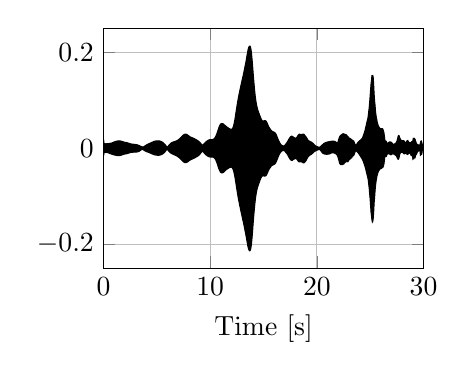
\begin{tikzpicture}

\begin{axis}[%
width=1.6in,
height=1.2in,
at={(0.758in,0.481in)},
scale only axis,
xmin=0,
xmax=30,
xmajorgrids,
ymin=-0.25,
ymax=0.25,
ymajorgrids,
xlabel={Time [s]},
axis background/.style={fill=white}
]
\addplot[fill=black,draw=black,forget plot] plot table[row sep=crcr]{%
2.08333333333333e-05	0.0181429386138916\\
0.0417454218822439	0.00981831550598145\\
0.0834700104311544	0.00948238372802734\\
0.125194598980065	0.00928175449371338\\
0.166919187528975	0.00922465324401855\\
0.208643776077886	0.00919592380523682\\
0.250368364626797	0.00919759273529053\\
0.292092953175707	0.00923550128936768\\
0.333817541724618	0.00927877426147461\\
0.375542130273528	0.00935649871826172\\
0.417266718822439	0.00944411754608154\\
0.458991307371349	0.00958895683288574\\
0.50071589592026	0.00970327854156494\\
0.54244048446917	0.00985097885131836\\
0.584165073018081	0.010007381439209\\
0.625889661566991	0.010167121887207\\
0.667614250115902	0.0103319883346558\\
0.709338838664812	0.0105338096618652\\
0.751063427213723	0.0107591152191162\\
0.792788015762633	0.0110471248626709\\
0.834512604311544	0.0113914012908936\\
0.876237192860454	0.0117802619934082\\
0.917961781409365	0.0121849775314331\\
0.959686369958275	0.0126172304153442\\
1.00141095850719	0.0130622386932373\\
1.0431355470561	0.0134444236755371\\
1.08486013560501	0.01375412940979\\
1.12658472415392	0.0140461921691895\\
1.16830931270283	0.0143270492553711\\
1.21003390125174	0.0145690441131592\\
1.25175848980065	0.014772891998291\\
1.29348307834956	0.0149348974227905\\
1.33520766689847	0.0150550603866577\\
1.37693225544738	0.015159010887146\\
1.41865684399629	0.0151675939559937\\
1.4603814325452	0.0152227878570557\\
1.50210602109411	0.0152052640914917\\
1.54383060964302	0.0151263475418091\\
1.58555519819193	0.0149624347686768\\
1.62727978674084	0.0147508382797241\\
1.66900437528975	0.0144839286804199\\
1.71072896383866	0.0141875743865967\\
1.75245355238758	0.013906717300415\\
1.79417814093649	0.0136110782623291\\
1.8359027294854	0.0133013725280762\\
1.87762731803431	0.0130418539047241\\
1.91935190658322	0.0127606391906738\\
1.96107649513213	0.012520432472229\\
2.00280108368104	0.0122427940368652\\
2.04452567222995	0.0120542049407959\\
2.08625026077886	0.0119724273681641\\
2.12797484932777	0.0119329690933228\\
2.16969943787668	0.0117537975311279\\
2.21142402642559	0.0113049745559692\\
2.2531486149745	0.0109944343566895\\
2.29487320352341	0.0107061862945557\\
2.33659779207232	0.0104308128356934\\
2.37832238062123	0.0101655721664429\\
2.42004696917014	0.00986766815185547\\
2.46177155771905	0.00956177711486816\\
2.50349614626796	0.0092771053314209\\
2.54522073481687	0.00905478000640869\\
2.58694532336579	0.00881576538085938\\
2.6286699119147	0.00863051414489746\\
2.67039450046361	0.00850450992584229\\
2.71211908901252	0.0083693265914917\\
2.75384367756143	0.00831413269042969\\
2.79556826611034	0.00819647312164307\\
2.83729285465925	0.00810885429382324\\
2.87901744320816	0.00798535346984863\\
2.92074203175707	0.00786435604095459\\
2.96246662030598	0.00775504112243652\\
3.00419120885489	0.00761902332305908\\
3.0459157974038	0.00745344161987305\\
3.08764038595271	0.00733506679534912\\
3.12936497450162	0.00713145732879639\\
3.17108956305053	0.00688385963439941\\
3.21281415159944	0.00660014152526855\\
3.25453874014835	0.00629806518554688\\
3.29626332869726	0.00598013401031494\\
3.33798791724618	0.00557184219360352\\
3.37971250579509	0.00512993335723877\\
3.421437094344	0.00457584857940674\\
3.46316168289291	0.00406599044799805\\
3.50488627144182	0.00371432304382324\\
3.54661085999073	0.00337004661560059\\
3.58833544853964	0.00308215618133545\\
3.63006003708855	0.0028533935546875\\
3.67178462563746	0.00265538692474365\\
3.71350921418637	0.00253880023956299\\
3.75523380273528	0.00263607501983643\\
3.79695839128419	0.00331485271453857\\
3.8386829798331	0.0040050745010376\\
3.88040756838201	0.00470507144927979\\
3.92213215693092	0.00538778305053711\\
3.96385674547983	0.00601017475128174\\
4.00558133402874	0.00653982162475586\\
4.04730592257765	0.00705873966217041\\
4.08903051112656	0.00755190849304199\\
4.13075509967547	0.00799787044525146\\
4.17247968822439	0.00844311714172363\\
4.2142042767733	0.00888705253601074\\
4.25592886532221	0.00932633876800537\\
4.29765345387112	0.00972950458526611\\
4.33937804242003	0.0101413726806641\\
4.38110263096894	0.0105501413345337\\
4.42282721951785	0.0109994411468506\\
4.46455180806676	0.0114316940307617\\
4.50627639661567	0.0118687152862549\\
4.54800098516458	0.0123001337051392\\
4.58972557371349	0.01271653175354\\
4.6314501622624	0.0131446123123169\\
4.67317475081131	0.0135660171508789\\
4.71489933936022	0.0139623880386353\\
4.75662392790913	0.0142995119094849\\
4.79834851645804	0.0145468711853027\\
4.84007310500695	0.0147733688354492\\
4.88179769355586	0.014928936958313\\
4.92352228210478	0.0150841474533081\\
4.96524687065368	0.0152616500854492\\
5.0069714592026	0.0152624845504761\\
5.04869604775151	0.0153963565826416\\
5.09042063630042	0.0153876543045044\\
5.13214522484933	0.0153646469116211\\
5.17386981339824	0.015326976776123\\
5.21559440194715	0.0151892900466919\\
5.25731899049606	0.0150249004364014\\
5.29904357904497	0.0147628784179688\\
5.34076816759388	0.0144513845443726\\
5.38249275614279	0.0140842199325562\\
5.4242173446917	0.0136476755142212\\
5.46594193324061	0.0131738185882568\\
5.50766652178952	0.0125408172607422\\
5.54939111033843	0.0119550228118896\\
5.59111569888734	0.0112673044204712\\
5.63284028743625	0.0104833841323853\\
5.67456487598516	0.00955593585968018\\
5.71628946453407	0.00849902629852295\\
5.75801405308299	0.0074155330657959\\
5.7997386416319	0.00631153583526611\\
5.84146323018081	0.00510704517364502\\
5.88318781872972	0.00393617153167725\\
5.92491240727863	0.00282895565032959\\
5.96663699582754	0.00194847583770752\\
6.00836158437645	0.00275373458862305\\
6.05008617292536	0.0039294958114624\\
6.09181076147427	0.00514364242553711\\
6.13353535002318	0.00633072853088379\\
6.17525993857209	0.00743377208709717\\
6.216984527121	0.00839316844940186\\
6.25870911566991	0.00930440425872803\\
6.30043370421882	0.0101140737533569\\
6.34215829276773	0.0107662677764893\\
6.38388288131664	0.0113470554351807\\
6.42560746986555	0.0118482112884521\\
6.46733205841446	0.0123203992843628\\
6.50905664696338	0.0127465724945068\\
6.55078123551229	0.0130656957626343\\
6.5925058240612	0.0133852958679199\\
6.63423041261011	0.0136781930923462\\
6.67595500115902	0.0139986276626587\\
6.71767958970793	0.0142853260040283\\
6.75940417825684	0.0145882368087769\\
6.80112876680575	0.0149731636047363\\
6.84285335535466	0.0153491497039795\\
6.88457794390357	0.0157651901245117\\
6.92630253245248	0.0162967443466187\\
6.96802712100139	0.0167956352233887\\
7.0097517095503	0.0174661874771118\\
7.05147629809921	0.0181162357330322\\
7.09320088664812	0.018841028213501\\
7.13492547519703	0.0196692943572998\\
7.17665006374594	0.0205473899841309\\
7.21837465229485	0.0214707851409912\\
7.26009924084376	0.0224095582962036\\
7.30182382939268	0.0234026908874512\\
7.34354841794159	0.0243393182754517\\
7.3852730064905	0.0253564119338989\\
7.42699759503941	0.0262609720230103\\
7.46872218358832	0.0271000862121582\\
7.51044677213723	0.0278606414794922\\
7.55217136068614	0.0284832715988159\\
7.59389594923505	0.0289143323898315\\
7.63562053778396	0.029173731803894\\
7.67734512633287	0.029242992401123\\
7.71906971488178	0.0291984081268311\\
7.76079430343069	0.0289905071258545\\
7.8025188919796	0.028531551361084\\
7.84424348052851	0.0280218124389648\\
7.88596806907742	0.0274125337600708\\
7.92769265762633	0.0267487764358521\\
7.96941724617524	0.026013970375061\\
8.01114183472416	0.0253177881240845\\
8.05286642327307	0.0246345996856689\\
8.09459101182198	0.0240037441253662\\
8.13631560037089	0.0234735012054443\\
8.1780401889198	0.0229911804199219\\
8.21976477746871	0.0225847959518433\\
8.26148936601762	0.0222088098526001\\
8.30321395456653	0.0218422412872314\\
8.34493854311544	0.0214892625808716\\
8.38666313166435	0.021141529083252\\
8.42838772021326	0.0207474231719971\\
8.47011230876217	0.0202984809875488\\
8.51183689731108	0.0198361873626709\\
8.55356148585999	0.0193321704864502\\
8.5952860744089	0.0187733173370361\\
8.63701066295781	0.0182367563247681\\
8.67873525150672	0.0177633762359619\\
8.72045984005563	0.0171844959259033\\
8.76218442860454	0.0166183710098267\\
8.80390901715345	0.0160551071166992\\
8.84563360570237	0.015450119972229\\
8.88735819425128	0.0148581266403198\\
8.92908278280018	0.0140950679779053\\
8.9708073713491	0.0132759809494019\\
9.01253195989801	0.012357234954834\\
9.05425654844692	0.0112653970718384\\
9.09598113699583	0.0102156400680542\\
9.13770572554474	0.00912904739379883\\
9.17943031409365	0.00804519653320313\\
9.22115490264256	0.00710666179656982\\
9.26287949119147	0.00655972957611084\\
9.30460407974038	0.006683349609375\\
9.34632866828929	0.007407546043396\\
9.3880532568382	0.00838303565979004\\
9.42977784538711	0.0093536376953125\\
9.47150243393602	0.0104529857635498\\
9.51322702248493	0.0113649368286133\\
9.55495161103384	0.0123004913330078\\
9.59667619958275	0.0131921768188477\\
9.63840078813166	0.013947606086731\\
9.68012537668058	0.0145976543426514\\
9.72184996522949	0.0152043104171753\\
9.7635745537784	0.0158047676086426\\
9.80529914232731	0.016348123550415\\
9.84702373087622	0.0167977809906006\\
9.88874831942513	0.0172429084777832\\
9.93047290797404	0.0175259113311768\\
9.97219749652295	0.017730712890625\\
10.0139220850719	0.0178829431533813\\
10.0556466736208	0.0179476737976074\\
10.0973712621697	0.0179698467254639\\
10.1390958507186	0.0179606676101685\\
10.1808204392675	0.0179910659790039\\
10.2225450278164	0.0181316137313843\\
10.2642696163653	0.0183707475662231\\
10.3059942049142	0.0187233686447144\\
10.3477187934631	0.019415020942688\\
10.3894433820121	0.020249605178833\\
10.431167970561	0.0213139057159424\\
10.4728925591099	0.022710919380188\\
10.5146171476588	0.0244239568710327\\
10.5563417362077	0.0264555215835571\\
10.5980663247566	0.0287165641784668\\
10.6397909133055	0.0312116146087646\\
10.6815155018544	0.0340604782104492\\
10.7232400904033	0.0369764566421509\\
10.7649646789523	0.039887547492981\\
10.8066892675012	0.0425577163696289\\
10.8484138560501	0.0450006723403931\\
10.890138444599	0.0471494197845459\\
10.9318630331479	0.0489104986190796\\
10.9735876216968	0.0501575469970703\\
11.0153122102457	0.0509358644485474\\
11.0570367987946	0.05133056640625\\
11.0987613873435	0.0514000654220581\\
11.1404859758924	0.0513108968734741\\
11.1822105644414	0.0510138273239136\\
11.2239351529903	0.0505356788635254\\
11.2656597415392	0.0497449636459351\\
11.3073843300881	0.0489338636398315\\
11.349108918637	0.0481431484222412\\
11.3908335071859	0.0472944974899292\\
11.4325580957348	0.0465856790542603\\
11.4742826842837	0.0457395315170288\\
11.5160072728326	0.0450065135955811\\
11.5577318613816	0.0442876815795898\\
11.5994564499305	0.0435512065887451\\
11.6411810384794	0.0428935289382935\\
11.6829056270283	0.04227614402771\\
11.7246302155772	0.0416744947433472\\
11.7663548041261	0.0411020517349243\\
11.808079392675	0.0405678749084473\\
11.8498039812239	0.0400964021682739\\
11.8915285697728	0.039612889289856\\
11.9332531583217	0.0393779277801514\\
11.9749777468707	0.0391607284545898\\
12.0167023354196	0.0395464897155762\\
12.0584269239685	0.0403308868408203\\
12.1001515125174	0.0414246320724487\\
12.1418761010663	0.0434789657592773\\
12.1836006896152	0.046017050743103\\
12.2253252781641	0.0495421886444092\\
12.267049866713	0.0540462732315063\\
12.3087744552619	0.0589500665664673\\
12.3504990438108	0.0645291805267334\\
12.3922236323598	0.0709797143936157\\
12.4339482209087	0.0772055387496948\\
12.4756728094576	0.0831716060638428\\
12.5173973980065	0.0890361070632935\\
12.5591219865554	0.0948562622070313\\
12.6008465751043	0.0999815464019775\\
12.6425711636532	0.105309963226318\\
12.6842957522021	0.109994530677795\\
12.726020340751	0.114959597587585\\
12.7677449293	0.119269251823425\\
12.8094695178489	0.123426556587219\\
12.8511941063978	0.127450466156006\\
12.8929186949467	0.132065773010254\\
12.9346432834956	0.136207699775696\\
12.9763678720445	0.140340328216553\\
13.0180924605934	0.144272685050964\\
13.0598170491423	0.148514747619629\\
13.1015416376912	0.15285861492157\\
13.1432662262401	0.15709924697876\\
13.1849908147891	0.161356449127197\\
13.226715403338	0.16622793674469\\
13.2684399918869	0.170778632164001\\
13.3101645804358	0.175296545028687\\
13.3518891689847	0.180025815963745\\
13.3936137575336	0.185588836669922\\
13.4353383460825	0.190938472747803\\
13.4770629346314	0.196236610412598\\
13.5187875231803	0.201432704925537\\
13.5605121117293	0.206299066543579\\
13.6022367002782	0.209556818008423\\
13.6439612888271	0.211467623710632\\
13.685685877376	0.212591648101807\\
13.7274104659249	0.212594151496887\\
13.7691350544738	0.210929751396179\\
13.8108596430227	0.206770896911621\\
13.8525842315716	0.200291275978088\\
13.8943088201205	0.191638708114624\\
13.9360334086694	0.180822372436523\\
13.9777579972184	0.169516563415527\\
14.0194825857673	0.157299280166626\\
14.0612071743162	0.145524978637695\\
14.1029317628651	0.134286284446716\\
14.144656351414	0.124222993850708\\
14.1863809399629	0.115064740180969\\
14.2281055285118	0.106799483299255\\
14.2698301170607	0.0998066663742065\\
14.3115547056096	0.0939657688140869\\
14.3532792941586	0.0890557765960693\\
14.3950038827075	0.0849928855895996\\
14.4367284712564	0.0814681053161621\\
14.4784530598053	0.078420877456665\\
14.5201776483542	0.0756738185882568\\
14.5619022369031	0.0731049776077271\\
14.603626825452	0.0705641508102417\\
14.6453514140009	0.0680527687072754\\
14.6870760025498	0.0655460357666016\\
14.7288005910988	0.0631619691848755\\
14.7705251796477	0.061133861541748\\
14.8122497681966	0.059224009513855\\
14.8539743567455	0.0578275918960571\\
14.8956989452944	0.0569607019424438\\
14.9374235338433	0.0565718412399292\\
14.9791481223922	0.0567365884780884\\
15.0208727109411	0.0569051504135132\\
15.06259729949	0.057193398475647\\
15.1043218880389	0.0573865175247192\\
15.1460464765879	0.0574783086776733\\
15.1877710651368	0.0571279525756836\\
15.2294956536857	0.0565847158432007\\
15.2712202422346	0.0549691915512085\\
15.3129448307835	0.0532348155975342\\
15.3546694193324	0.051118016242981\\
15.3963940078813	0.0490202903747559\\
15.4381185964302	0.0468697547912598\\
15.4798431849791	0.045029878616333\\
15.521567773528	0.0431989431381226\\
15.563292362077	0.0417073965072632\\
15.6050169506259	0.0404326915740967\\
15.6467415391748	0.0390024185180664\\
15.6884661277237	0.0379331111907959\\
15.7301907162726	0.0368587970733643\\
15.7719153048215	0.035975456237793\\
15.8136398933704	0.0350592136383057\\
15.8553644819193	0.0345426797866821\\
15.8970890704682	0.0341147184371948\\
15.9388136590172	0.0337724685668945\\
15.9805382475661	0.0333970785140991\\
16.022262836115	0.0329580307006836\\
16.0639874246639	0.0321637392044067\\
16.1057120132128	0.0311347246170044\\
16.1474366017617	0.0299307107925415\\
16.1891611903106	0.0278295278549194\\
16.2308857788595	0.0256993770599365\\
16.2726103674084	0.0232733488082886\\
16.3143349559573	0.0209442377090454\\
16.3560595445063	0.0186095237731934\\
16.3977841330552	0.0164110660552979\\
16.4395087216041	0.0143883228302002\\
16.481233310153	0.0125398635864258\\
16.5229578987019	0.0109268426895142\\
16.5646824872508	0.00943207740783691\\
16.6064070757997	0.00811886787414551\\
16.6481316643486	0.00709044933319092\\
16.6898562528975	0.00629234313964844\\
16.7315808414465	0.00571024417877197\\
16.7733054299954	0.00532305240631104\\
16.8150300185443	0.00502550601959229\\
16.8567546070932	0.00477826595306396\\
16.8984791956421	0.00490677356719971\\
16.940203784191	0.00500261783599854\\
16.9819283727399	0.00551116466522217\\
17.0236529612888	0.00693738460540771\\
17.0653775498377	0.00799381732940674\\
17.1071021383867	0.0093151330947876\\
17.1488267269356	0.0102335214614868\\
17.1905513154845	0.0115920305252075\\
17.2322759040334	0.0131574869155884\\
17.2740004925823	0.0146949291229248\\
17.3157250811312	0.0163867473602295\\
17.3574496696801	0.0181008577346802\\
17.399174258229	0.0195778608322144\\
17.4408988467779	0.0210890769958496\\
17.4826234353268	0.022479772567749\\
17.5243480238758	0.0236889123916626\\
17.5660726124247	0.0245449542999268\\
17.6077972009736	0.0249673128128052\\
17.6495217895225	0.0250524282455444\\
17.6912463780714	0.0247505903244019\\
17.7329709666203	0.0242820978164673\\
17.7746955551692	0.0233075618743896\\
17.8164201437181	0.0227642059326172\\
17.858144732267	0.0220650434494019\\
17.8998693208159	0.0215951204299927\\
17.9415939093649	0.0210493803024292\\
17.9833184979138	0.0209370851516724\\
18.0250430864627	0.0211421251296997\\
18.0667676750116	0.0216693878173828\\
18.1084922635605	0.0226044654846191\\
18.1502168521094	0.0235614776611328\\
18.1919414406583	0.0250465869903564\\
18.2336660292072	0.0265630483627319\\
18.2753906177561	0.0277305841445923\\
18.3171152063051	0.0287457704544067\\
18.358839794854	0.0291450023651123\\
18.4005643834029	0.0291095972061157\\
18.4422889719518	0.0286276340484619\\
18.4840135605007	0.0283635854721069\\
18.5257381490496	0.0279011726379395\\
18.5674627375985	0.0284152030944824\\
18.6091873261474	0.0289162397384644\\
18.6509119146963	0.029058575630188\\
18.6926365032453	0.0292384624481201\\
18.7343610917942	0.0291332006454468\\
18.7760856803431	0.0291461944580078\\
18.817810268892	0.0281885862350464\\
18.8595348574409	0.02684485912323\\
18.9012594459898	0.0255180597305298\\
18.9429840345387	0.0244811773300171\\
18.9847086230876	0.0234601497650146\\
19.0264332116365	0.0220894813537598\\
19.0681578001854	0.0204522609710693\\
19.1098823887344	0.0188456773757935\\
19.1516069772833	0.0171926021575928\\
19.1933315658322	0.0162808895111084\\
19.2350561543811	0.0156338214874268\\
19.27678074293	0.0148259401321411\\
19.3185053314789	0.014142632484436\\
19.3602299200278	0.0135996341705322\\
19.4019545085767	0.0133801698684692\\
19.4436790971256	0.0130627155303955\\
19.4854036856745	0.0126312971115112\\
19.5271282742235	0.0120033025741577\\
19.5688528627724	0.0112236738204956\\
19.6105774513213	0.0104175806045532\\
19.6523020398702	0.00954711437225342\\
19.6940266284191	0.00854158401489258\\
19.735751216968	0.00752699375152588\\
19.7774758055169	0.00662863254547119\\
19.8192003940658	0.00591504573822021\\
19.8609249826147	0.00523173809051514\\
19.9026495711637	0.0045616626739502\\
19.9443741597126	0.00404226779937744\\
19.9860987482615	0.00355184078216553\\
20.0278233368104	0.00309014320373535\\
20.0695479253593	0.00289607048034668\\
20.1112725139082	0.00259554386138916\\
20.1529971024571	0.00220882892608643\\
20.194721691006	0.00174784660339355\\
20.2364462795549	0.00176405906677246\\
20.2781708681038	0.00237834453582764\\
20.3198954566528	0.00308012962341309\\
20.3616200452017	0.00385606288909912\\
20.4033446337506	0.00467050075531006\\
20.4450692222995	0.00547373294830322\\
20.4867938108484	0.006400465965271\\
20.5285183993973	0.00724613666534424\\
20.5702429879462	0.00812721252441406\\
20.6119675764951	0.00894665718078613\\
20.653692165044	0.00969398021697998\\
20.695416753593	0.0102465152740479\\
20.7371413421419	0.0107783079147339\\
20.7788659306908	0.0112481117248535\\
20.8205905192397	0.0116442441940308\\
20.8623151077886	0.01198410987854\\
20.9040396963375	0.012417197227478\\
20.9457642848864	0.0125412940979004\\
20.9874888734353	0.0128133296966553\\
21.0292134619842	0.0130845308303833\\
21.0709380505331	0.0132529735565186\\
21.1126626390821	0.0134599208831787\\
21.154387227631	0.0136171579360962\\
21.1961118161799	0.0137416124343872\\
21.2378364047288	0.013939380645752\\
21.2795609932777	0.014137864112854\\
21.3212855818266	0.0143916606903076\\
21.3630101703755	0.0145068168640137\\
21.4047347589244	0.0146383047103882\\
21.4464593474733	0.0146561861038208\\
21.4881839360223	0.0147119760513306\\
21.5299085245712	0.0146753787994385\\
21.5716331131201	0.0145899057388306\\
21.613357701669	0.0144120454788208\\
21.6550822902179	0.0142247676849365\\
21.6968068787668	0.0139384269714355\\
21.7385314673157	0.013425350189209\\
21.7802560558646	0.0128157138824463\\
21.8219806444135	0.0119717121124268\\
21.8637052329624	0.0108844041824341\\
21.9054298215114	0.00947654247283936\\
21.9471544100603	0.0106815099716187\\
21.9888789986092	0.0139356851577759\\
22.0306035871581	0.0172305107116699\\
22.072328175707	0.0200293064117432\\
22.1140527642559	0.0227704048156738\\
22.1557773528048	0.0246222019195557\\
22.1975019413537	0.0260888338088989\\
22.2392265299026	0.0269640684127808\\
22.2809511184516	0.0277798175811768\\
22.3226757070005	0.0281111001968384\\
22.3644002955494	0.02862548828125\\
22.4061248840983	0.0298867225646973\\
22.4478494726472	0.0299409627914429\\
22.4895740611961	0.0300390720367432\\
22.531298649745	0.0296164751052856\\
22.5730232382939	0.0294182300567627\\
22.6147478268428	0.0292960405349731\\
22.6564724153917	0.0285204648971558\\
22.6981970039407	0.0279887914657593\\
22.7399215924896	0.026756763458252\\
22.7816461810385	0.0276104211807251\\
22.8233707695874	0.0258729457855225\\
22.8650953581363	0.025011420249939\\
22.9068199466852	0.0239888429641724\\
22.9485445352341	0.0234851837158203\\
22.990269123783	0.0218654870986938\\
23.0319937123319	0.0209083557128906\\
23.0737183008809	0.0205870866775513\\
23.1154428894298	0.0203926563262939\\
23.1571674779787	0.019506573677063\\
23.1988920665276	0.0189449787139893\\
23.2406166550765	0.0177148580551147\\
23.2823412436254	0.0172977447509766\\
23.3240658321743	0.0163909196853638\\
23.3657904207232	0.0161864757537842\\
23.4075150092721	0.015525221824646\\
23.449239597821	0.014864444732666\\
23.49096418637	0.012748122215271\\
23.5326887749189	0.0103925466537476\\
23.5744133634678	0.00771594047546387\\
23.6161379520167	0.00587379932403564\\
23.6578625405656	0.00552535057067871\\
23.6995871291145	0.00676417350769043\\
23.7413117176634	0.00831508636474609\\
23.7830363062123	0.00996637344360352\\
23.8247608947612	0.0112411975860596\\
23.8664854833102	0.0123852491378784\\
23.9082100718591	0.0134469270706177\\
23.949934660408	0.0143195390701294\\
23.9916592489569	0.0151535272598267\\
24.0333838375058	0.0158790349960327\\
24.0751084260547	0.0166734457015991\\
24.1168330146036	0.0175095796585083\\
24.1585576031525	0.018479585647583\\
24.2002821917014	0.0192961692810059\\
24.2420067802503	0.0202317237854004\\
24.2837313687993	0.021916389465332\\
24.3254559573482	0.0242879390716553\\
24.3671805458971	0.0267579555511475\\
24.408905134446	0.0292876958847046\\
24.4506297229949	0.0321053266525269\\
24.4923543115438	0.0353796482086182\\
24.5340789000927	0.0388656854629517\\
24.5758034886416	0.0428327322006226\\
24.6175280771905	0.0469703674316406\\
24.6592526657395	0.0512353181838989\\
24.7009772542884	0.0551902055740356\\
24.7427018428373	0.0587172508239746\\
24.7844264313862	0.0624885559082031\\
24.8261510199351	0.0693908929824829\\
24.867875608484	0.0772602558135986\\
24.9096001970329	0.0853687524795532\\
24.9513247855818	0.0968271493911743\\
24.9930493741307	0.108737111091614\\
25.0347739626796	0.121615767478943\\
25.0764985512286	0.133149027824402\\
25.1182231397775	0.14117157459259\\
25.1599477283264	0.151021957397461\\
25.2016723168753	0.151101231575012\\
25.2433969054242	0.151412844657898\\
25.2851214939731	0.145847797393799\\
25.326846082522	0.128899931907654\\
25.3685706710709	0.111058950424194\\
25.4102952596198	0.0976966619491577\\
25.4520198481687	0.0893508195877075\\
25.4937444367177	0.0765688419342041\\
25.5354690252666	0.0692602396011353\\
25.5771936138155	0.0631908178329468\\
25.6189182023644	0.0591845512390137\\
25.6606427909133	0.053180456161499\\
25.7023673794622	0.0502039194107056\\
25.7440919680111	0.0475097894668579\\
25.78581655656	0.0455487966537476\\
25.8275411451089	0.043721079826355\\
25.8692657336579	0.0425406694412231\\
25.9109903222068	0.0414412021636963\\
25.9527149107557	0.0406630039215088\\
25.9944394993046	0.0404994487762451\\
26.0361640878535	0.0406029224395752\\
26.0778886764024	0.0408178567886353\\
26.1196132649513	0.0408438444137573\\
26.1613378535002	0.0403792858123779\\
26.2030624420491	0.0384087562561035\\
26.2447870305981	0.0354056358337402\\
26.286511619147	0.0315598249435425\\
26.3282362076959	0.0250397920608521\\
26.3699607962448	0.0174821615219116\\
26.4116853847937	0.0142930746078491\\
26.4534099733426	0.0146453380584717\\
26.4951345618915	0.0144370794296265\\
26.5368591504404	0.0122486352920532\\
26.5785837389893	0.0104124546051025\\
26.6203083275383	0.00970661640167236\\
26.6620329160872	0.0103627443313599\\
26.7037575046361	0.0113061666488647\\
26.745482093185	0.012203574180603\\
26.7872066817339	0.0128524303436279\\
26.8289312702828	0.0130819082260132\\
26.8706558588317	0.0130194425582886\\
26.9123804473806	0.0128352642059326\\
26.9541050359295	0.0126463174819946\\
26.9958296244784	0.0120117664337158\\
27.0375542130274	0.0108309984207153\\
27.0792788015763	0.00957667827606201\\
27.1210033901252	0.00817191600799561\\
27.1627279786741	0.00803875923156738\\
27.204452567223	0.00838303565979004\\
27.2461771557719	0.00871133804321289\\
27.2879017443208	0.00894832611083984\\
27.3296263328697	0.00926840305328369\\
27.3713509214186	0.00976073741912842\\
27.4130755099675	0.0109186172485352\\
27.4548000985165	0.0123889446258545\\
27.4965246870654	0.01393723487854\\
27.5382492756143	0.0170615911483765\\
27.5799738641632	0.0210994482040405\\
27.6216984527121	0.0251799821853638\\
27.663423041261	0.0265043973922729\\
27.7051476298099	0.0259286165237427\\
27.7468722183588	0.0226286649703979\\
27.7885968069077	0.0206558704376221\\
27.8303213954567	0.0187374353408813\\
27.8720459840056	0.017424464225769\\
27.9137705725545	0.016254186630249\\
27.9554951611034	0.0158206224441528\\
27.9972197496523	0.0154150724411011\\
28.0389443382012	0.0155537128448486\\
28.0806689267501	0.015681266784668\\
28.122393515299	0.0157088041305542\\
28.1641181038479	0.0152533054351807\\
28.2058426923968	0.0140600204467773\\
28.2475672809458	0.0119315385818481\\
28.2892918694947	0.0118236541748047\\
28.3310164580436	0.0121282339096069\\
28.3727410465925	0.0123680830001831\\
28.4144656351414	0.0139719247817993\\
28.4561902236903	0.0155477523803711\\
28.4979148122392	0.0160571336746216\\
28.5396394007881	0.0152674913406372\\
28.581363989337	0.013501763343811\\
28.623088577886	0.0121248960494995\\
28.6648131664349	0.0115351676940918\\
28.7065377549838	0.0114558935165405\\
28.7482623435327	0.0115314722061157\\
28.7899869320816	0.0109808444976807\\
28.8317115206305	0.0124373435974121\\
28.8734361091794	0.0134687423706055\\
28.9151606977283	0.0131791830062866\\
28.9568852862772	0.0124815702438354\\
28.9986098748261	0.0159767866134644\\
29.0403344633751	0.0204752683639526\\
29.082059051924	0.0199533700942993\\
29.1237836404729	0.0171099901199341\\
29.1655082290218	0.0196442604064941\\
29.2072328175707	0.018378734588623\\
29.2489574061196	0.0146825313568115\\
29.2906819946685	0.0125558376312256\\
29.3324065832174	0.00908064842224121\\
29.3741311717663	0.00805020332336426\\
29.4158557603153	0.00818371772766113\\
29.4575803488642	0.00766909122467041\\
29.4993049374131	0.00696444511413574\\
29.541029525962	0.00585794448852539\\
29.5827541145109	0.00566279888153076\\
29.6244787030598	0.00570785999298096\\
29.6662032916087	0.00787365436553955\\
29.7079278801576	0.0109878778457642\\
29.7496524687065	0.014776349067688\\
29.7913770572554	0.0149766206741333\\
29.8331016458044	0.0116641521453857\\
29.8748262343533	0.00800597667694092\\
29.9165508229022	0.004416823387146\\
29.9582754114511	0.00193178653717041\\
30	0.00354182720184326\\
}
\closedcycle;
\addplot[fill=black,draw=black,forget plot] plot table[row sep=crcr]{%
2.08333333333333e-05	-0.0156445503234863\\
0.0417454218822439	-0.00975942611694336\\
0.0834700104311544	-0.00913405418395996\\
0.125194598980065	-0.00892078876495361\\
0.166919187528975	-0.00880742073059082\\
0.208643776077886	-0.00872552394866943\\
0.250368364626797	-0.00868713855743408\\
0.292092953175707	-0.00875759124755859\\
0.333817541724618	-0.00887036323547363\\
0.375542130273528	-0.00913524627685547\\
0.417266718822439	-0.00939607620239258\\
0.458991307371349	-0.00966882705688477\\
0.50071589592026	-0.0099865198135376\\
0.54244048446917	-0.0103727579116821\\
0.584165073018081	-0.0107719898223877\\
0.625889661566991	-0.0111725330352783\\
0.667614250115902	-0.0115311145782471\\
0.709338838664812	-0.0118782520294189\\
0.751063427213723	-0.0122215747833252\\
0.792788015762633	-0.0125161409378052\\
0.834512604311544	-0.0128002166748047\\
0.876237192860454	-0.0130515098571777\\
0.917961781409365	-0.0133438110351563\\
0.959686369958275	-0.0136183500289917\\
1.00141095850719	-0.0138192176818848\\
1.0431355470561	-0.0140774250030518\\
1.08486013560501	-0.0142751932144165\\
1.12658472415392	-0.0144971609115601\\
1.16830931270283	-0.0147165060043335\\
1.21003390125174	-0.0149143934249878\\
1.25175848980065	-0.015013575553894\\
1.29348307834956	-0.0151480436325073\\
1.33520766689847	-0.0152536630630493\\
1.37693225544738	-0.0152581930160522\\
1.41865684399629	-0.0152781009674072\\
1.4603814325452	-0.0152415037155151\\
1.50210602109411	-0.0151500701904297\\
1.54383060964302	-0.0150383710861206\\
1.58555519819193	-0.0148442983627319\\
1.62727978674084	-0.0146211385726929\\
1.66900437528975	-0.0143373012542725\\
1.71072896383866	-0.0140464305877686\\
1.75245355238758	-0.013671875\\
1.79417814093649	-0.0133310556411743\\
1.8359027294854	-0.013018012046814\\
1.87762731803431	-0.0126738548278809\\
1.91935190658322	-0.0124160051345825\\
1.96107649513213	-0.0121539831161499\\
2.00280108368104	-0.0119320154190063\\
2.04452567222995	-0.0117262601852417\\
2.08625026077886	-0.0116888284683228\\
2.12797484932777	-0.0116533041000366\\
2.16969943787668	-0.0115129947662354\\
2.21142402642559	-0.0110875368118286\\
2.2531486149745	-0.0107666254043579\\
2.29487320352341	-0.0104871988296509\\
2.33659779207232	-0.010197639465332\\
2.37832238062123	-0.00992798805236816\\
2.42004696917014	-0.00962507724761963\\
2.46177155771905	-0.00936400890350342\\
2.50349614626796	-0.00912153720855713\\
2.54522073481687	-0.00890958309173584\\
2.58694532336579	-0.00873839855194092\\
2.6286699119147	-0.00856375694274902\\
2.67039450046361	-0.00847268104553223\\
2.71211908901252	-0.0083308219909668\\
2.75384367756143	-0.00829923152923584\\
2.79556826611034	-0.00824832916259766\\
2.83729285465925	-0.00820529460906982\\
2.87901744320816	-0.00811970233917236\\
2.92074203175707	-0.0080564022064209\\
2.96246662030598	-0.00800824165344238\\
3.00419120885489	-0.00794577598571777\\
3.0459157974038	-0.00790023803710938\\
3.08764038595271	-0.00780773162841797\\
3.12936497450162	-0.00770246982574463\\
3.17108956305053	-0.00749599933624268\\
3.21281415159944	-0.00731158256530762\\
3.25453874014835	-0.00700497627258301\\
3.29626332869726	-0.00666439533233643\\
3.33798791724618	-0.00625336170196533\\
3.37971250579509	-0.00571608543395996\\
3.421437094344	-0.00500726699829102\\
3.46316168289291	-0.0043179988861084\\
3.50488627144182	-0.00365817546844482\\
3.54661085999073	-0.00295770168304443\\
3.58833544853964	-0.00228428840637207\\
3.63006003708855	-0.00207078456878662\\
3.67178462563746	-0.00253427028656006\\
3.71350921418637	-0.00313544273376465\\
3.75523380273528	-0.00370323657989502\\
3.79695839128419	-0.00426912307739258\\
3.8386829798331	-0.00482392311096191\\
3.88040756838201	-0.00538480281829834\\
3.92213215693092	-0.00585043430328369\\
3.96385674547983	-0.00628888607025146\\
4.00558133402874	-0.00675547122955322\\
4.04730592257765	-0.00715041160583496\\
4.08903051112656	-0.00753092765808105\\
4.13075509967547	-0.00787448883056641\\
4.17247968822439	-0.00823116302490234\\
4.2142042767733	-0.0086216926574707\\
4.25592886532221	-0.00896334648132324\\
4.29765345387112	-0.00932466983795166\\
4.33937804242003	-0.00967597961425781\\
4.38110263096894	-0.010036826133728\\
4.42282721951785	-0.0104019641876221\\
4.46455180806676	-0.0108225345611572\\
4.50627639661567	-0.0112348794937134\\
4.54800098516458	-0.0116481781005859\\
4.58972557371349	-0.0120593309402466\\
4.6314501622624	-0.0124427080154419\\
4.67317475081131	-0.012823224067688\\
4.71489933936022	-0.013271689414978\\
4.75662392790913	-0.0135663747787476\\
4.79834851645804	-0.0137753486633301\\
4.84007310500695	-0.0139385461807251\\
4.88179769355586	-0.0141421556472778\\
4.92352228210478	-0.0142583847045898\\
4.96524687065368	-0.014370322227478\\
5.0069714592026	-0.0144532918930054\\
5.04869604775151	-0.0145694017410278\\
5.09042063630042	-0.0146268606185913\\
5.13214522484933	-0.0146278142929077\\
5.17386981339824	-0.0145910978317261\\
5.21559440194715	-0.0145310163497925\\
5.25731899049606	-0.014384388923645\\
5.29904357904497	-0.0141700506210327\\
5.34076816759388	-0.0138554573059082\\
5.38249275614279	-0.0135565996170044\\
5.4242173446917	-0.0132004022598267\\
5.46594193324061	-0.012775182723999\\
5.50766652178952	-0.0122224092483521\\
5.54939111033843	-0.011670708656311\\
5.59111569888734	-0.0110591650009155\\
5.63284028743625	-0.0103219747543335\\
5.67456487598516	-0.00942182540893555\\
5.71628946453407	-0.00847983360290527\\
5.75801405308299	-0.00744080543518066\\
5.7997386416319	-0.00624382495880127\\
5.84146323018081	-0.00501430034637451\\
5.88318781872972	-0.00372219085693359\\
5.92491240727863	-0.00244033336639404\\
5.96663699582754	-0.00204348564147949\\
6.00836158437645	-0.00318145751953125\\
6.05008617292536	-0.004355788230896\\
6.09181076147427	-0.00548160076141357\\
6.13353535002318	-0.00659275054931641\\
6.17525993857209	-0.00756180286407471\\
6.216984527121	-0.00850939750671387\\
6.25870911566991	-0.00929915904998779\\
6.30043370421882	-0.00996851921081543\\
6.34215829276773	-0.0105955600738525\\
6.38388288131664	-0.0111247301101685\\
6.42560746986555	-0.0116086006164551\\
6.46733205841446	-0.0120513439178467\\
6.50905664696338	-0.0124642848968506\\
6.55078123551229	-0.0128757953643799\\
6.5925058240612	-0.0133146047592163\\
6.63423041261011	-0.013680100440979\\
6.67595500115902	-0.0140740871429443\\
6.71767958970793	-0.0144442319869995\\
6.75940417825684	-0.0149235725402832\\
6.80112876680575	-0.0153471231460571\\
6.84285335535466	-0.0157897472381592\\
6.88457794390357	-0.0163278579711914\\
6.92630253245248	-0.0167744159698486\\
6.96802712100139	-0.0174590349197388\\
7.0097517095503	-0.0181128978729248\\
7.05147629809921	-0.0188889503479004\\
7.09320088664812	-0.019629955291748\\
7.13492547519703	-0.0204325914382935\\
7.17665006374594	-0.0212842226028442\\
7.21837465229485	-0.0222164392471313\\
7.26009924084376	-0.0231560468673706\\
7.30182382939268	-0.0240943431854248\\
7.34354841794159	-0.0250568389892578\\
7.3852730064905	-0.0259822607040405\\
7.42699759503941	-0.0269285440444946\\
7.46872218358832	-0.0277633666992188\\
7.51044677213723	-0.0285277366638184\\
7.55217136068614	-0.029197096824646\\
7.59389594923505	-0.0296359062194824\\
7.63562053778396	-0.0298813581466675\\
7.67734512633287	-0.029988169670105\\
7.71906971488178	-0.0299688577651978\\
7.76079430343069	-0.0298526287078857\\
7.8025188919796	-0.0294086933135986\\
7.84424348052851	-0.0289188623428345\\
7.88596806907742	-0.0283664464950562\\
7.92769265762633	-0.0275536775588989\\
7.96941724617524	-0.026883602142334\\
8.01114183472416	-0.0261441469192505\\
8.05286642327307	-0.0254770517349243\\
8.09459101182198	-0.0248786211013794\\
8.13631560037089	-0.0243445634841919\\
8.1780401889198	-0.023837685585022\\
8.21976477746871	-0.0233962535858154\\
8.26148936601762	-0.0230287313461304\\
8.30321395456653	-0.0226564407348633\\
8.34493854311544	-0.0222442150115967\\
8.38666313166435	-0.0218396186828613\\
8.42838772021326	-0.0213813781738281\\
8.47011230876217	-0.0209271907806396\\
8.51183689731108	-0.0204285383224487\\
8.55356148585999	-0.0199986696243286\\
8.5952860744089	-0.0194693803787231\\
8.63701066295781	-0.0188759565353394\\
8.67873525150672	-0.0184199810028076\\
8.72045984005563	-0.0178499221801758\\
8.76218442860454	-0.0173376798629761\\
8.80390901715345	-0.0167642831802368\\
8.84563360570237	-0.0160950422286987\\
8.88735819425128	-0.0154263973236084\\
8.92908278280018	-0.0146489143371582\\
8.9708073713491	-0.0137952566146851\\
9.01253195989801	-0.0127676725387573\\
9.05425654844692	-0.0116562843322754\\
9.09598113699583	-0.01051926612854\\
9.13770572554474	-0.00927376747131348\\
9.17943031409365	-0.00805139541625977\\
9.22115490264256	-0.0069422721862793\\
9.26287949119147	-0.00629758834838867\\
9.30460407974038	-0.00673818588256836\\
9.34632866828929	-0.00754570960998535\\
9.3880532568382	-0.00857651233673096\\
9.42977784538711	-0.00970268249511719\\
9.47150243393602	-0.0107744932174683\\
9.51322702248493	-0.011803150177002\\
9.55495161103384	-0.0126858949661255\\
9.59667619958275	-0.0135624408721924\\
9.63840078813166	-0.014382004737854\\
9.68012537668058	-0.0150749683380127\\
9.72184996522949	-0.0157070159912109\\
9.7635745537784	-0.0163074731826782\\
9.80529914232731	-0.0168285369873047\\
9.84702373087622	-0.0173298120498657\\
9.88874831942513	-0.0177673101425171\\
9.93047290797404	-0.0180290937423706\\
9.97219749652295	-0.0181993246078491\\
10.0139220850719	-0.0182913541793823\\
10.0556466736208	-0.0183722972869873\\
10.0973712621697	-0.0183372497558594\\
10.1390958507186	-0.0183314085006714\\
10.1808204392675	-0.0182371139526367\\
10.2225450278164	-0.0182504653930664\\
10.2642696163653	-0.0184223651885986\\
10.3059942049142	-0.0188477039337158\\
10.3477187934631	-0.019378662109375\\
10.3894433820121	-0.0201623439788818\\
10.431167970561	-0.0212167501449585\\
10.4728925591099	-0.0226330757141113\\
10.5146171476588	-0.0242002010345459\\
10.5563417362077	-0.0262751579284668\\
10.5980663247566	-0.0285011529922485\\
10.6397909133055	-0.0310791730880737\\
10.6815155018544	-0.0337928533554077\\
10.7232400904033	-0.0366888046264648\\
10.7649646789523	-0.0395543575286865\\
10.8066892675012	-0.0422680377960205\\
10.8484138560501	-0.0447573661804199\\
10.890138444599	-0.0468313694000244\\
10.9318630331479	-0.0485771894454956\\
10.9735876216968	-0.0499056577682495\\
11.0153122102457	-0.0506936311721802\\
11.0570367987946	-0.051161527633667\\
11.0987613873435	-0.0512508153915405\\
11.1404859758924	-0.0511727333068848\\
11.1822105644414	-0.0508694648742676\\
11.2239351529903	-0.0504333972930908\\
11.2656597415392	-0.0496697425842285\\
11.3073843300881	-0.0486760139465332\\
11.349108918637	-0.0480283498764038\\
11.3908335071859	-0.0470601320266724\\
11.4325580957348	-0.0461342334747314\\
11.4742826842837	-0.0452500581741333\\
11.5160072728326	-0.044459342956543\\
11.5577318613816	-0.0436632633209229\\
11.5994564499305	-0.0430549383163452\\
11.6411810384794	-0.0425050258636475\\
11.6829056270283	-0.0419497489929199\\
11.7246302155772	-0.0413506031036377\\
11.7663548041261	-0.0408295392990112\\
11.808079392675	-0.0404314994812012\\
11.8498039812239	-0.0399967432022095\\
11.8915285697728	-0.0397055149078369\\
11.9332531583217	-0.0394241809844971\\
11.9749777468707	-0.0393775701522827\\
12.0167023354196	-0.0398836135864258\\
12.0584269239685	-0.0405541658401489\\
12.1001515125174	-0.0421191453933716\\
12.1418761010663	-0.0439504384994507\\
12.1836006896152	-0.0464245080947876\\
12.2253252781641	-0.050078272819519\\
12.267049866713	-0.0542898178100586\\
12.3087744552619	-0.0588688850402832\\
12.3504990438108	-0.0644247531890869\\
12.3922236323598	-0.0702184438705444\\
12.4339482209087	-0.0763936042785645\\
12.4756728094576	-0.0830105543136597\\
12.5173973980065	-0.0881602764129639\\
12.5591219865554	-0.0941743850708008\\
12.6008465751043	-0.0994385480880737\\
12.6425711636532	-0.105164170265198\\
12.6842957522021	-0.109508991241455\\
12.726020340751	-0.114504933357239\\
12.7677449293	-0.119225740432739\\
12.8094695178489	-0.123663067817688\\
12.8511941063978	-0.128068208694458\\
12.8929186949467	-0.132378697395325\\
12.9346432834956	-0.137018799781799\\
12.9763678720445	-0.140941858291626\\
13.0180924605934	-0.145238518714905\\
13.0598170491423	-0.149763822555542\\
13.1015416376912	-0.153231024742126\\
13.1432662262401	-0.157874822616577\\
13.1849908147891	-0.16230583190918\\
13.226715403338	-0.167088270187378\\
13.2684399918869	-0.171908617019653\\
13.3101645804358	-0.176697134971619\\
13.3518891689847	-0.181561231613159\\
13.3936137575336	-0.18658971786499\\
13.4353383460825	-0.191940665245056\\
13.4770629346314	-0.197444915771484\\
13.5187875231803	-0.202711224555969\\
13.5605121117293	-0.206946015357971\\
13.6022367002782	-0.210256695747375\\
13.6439612888271	-0.212435603141785\\
13.685685877376	-0.213632106781006\\
13.7274104659249	-0.213499426841736\\
13.7691350544738	-0.211671113967896\\
13.8108596430227	-0.207690715789795\\
13.8525842315716	-0.201473593711853\\
13.8943088201205	-0.192561626434326\\
13.9360334086694	-0.181859970092773\\
13.9777579972184	-0.169991731643677\\
14.0194825857673	-0.15757167339325\\
14.0612071743162	-0.145878553390503\\
14.1029317628651	-0.134459495544434\\
14.144656351414	-0.12414824962616\\
14.1863809399629	-0.115036487579346\\
14.2281055285118	-0.106583595275879\\
14.2698301170607	-0.0996133089065552\\
14.3115547056096	-0.093874454498291\\
14.3532792941586	-0.0889596939086914\\
14.3950038827075	-0.0847424268722534\\
14.4367284712564	-0.0813336372375488\\
14.4784530598053	-0.0783452987670898\\
14.5201776483542	-0.0755771398544312\\
14.5619022369031	-0.0730820894241333\\
14.603626825452	-0.0705368518829346\\
14.6453514140009	-0.0678775310516357\\
14.6870760025498	-0.0654098987579346\\
14.7288005910988	-0.0632065534591675\\
14.7705251796477	-0.0612145662307739\\
14.8122497681966	-0.059637188911438\\
14.8539743567455	-0.05840003490448\\
14.8956989452944	-0.0575379133224487\\
14.9374235338433	-0.0572346448898315\\
14.9791481223922	-0.0574187040328979\\
15.0208727109411	-0.0576047897338867\\
15.06259729949	-0.057861328125\\
15.1043218880389	-0.0581213235855103\\
15.1460464765879	-0.0579477548599243\\
15.1877710651368	-0.057590126991272\\
15.2294956536857	-0.0568358898162842\\
15.2712202422346	-0.0554056167602539\\
15.3129448307835	-0.0536926984786987\\
15.3546694193324	-0.0514771938323975\\
15.3963940078813	-0.0494018793106079\\
15.4381185964302	-0.0473421812057495\\
15.4798431849791	-0.0454704761505127\\
15.521567773528	-0.0436441898345947\\
15.563292362077	-0.0420583486557007\\
15.6050169506259	-0.040719747543335\\
15.6467415391748	-0.0396767854690552\\
15.6884661277237	-0.0382914543151855\\
15.7301907162726	-0.0371015071868896\\
15.7719153048215	-0.0364335775375366\\
15.8136398933704	-0.0356283187866211\\
15.8553644819193	-0.0351072549819946\\
15.8970890704682	-0.034555196762085\\
15.9388136590172	-0.0341346263885498\\
15.9805382475661	-0.0338345766067505\\
16.022262836115	-0.0332046747207642\\
16.0639874246639	-0.0325386524200439\\
16.1057120132128	-0.0311926603317261\\
16.1474366017617	-0.0300180912017822\\
16.1891611903106	-0.0277334451675415\\
16.2308857788595	-0.0257387161254883\\
16.2726103674084	-0.0233829021453857\\
16.3143349559573	-0.0210640430450439\\
16.3560595445063	-0.0186415910720825\\
16.3977841330552	-0.0163822174072266\\
16.4395087216041	-0.0143485069274902\\
16.481233310153	-0.012478232383728\\
16.5229578987019	-0.0108493566513062\\
16.5646824872508	-0.00939023494720459\\
16.6064070757997	-0.00812149047851563\\
16.6481316643486	-0.00704586505889893\\
16.6898562528975	-0.00622844696044922\\
16.7315808414465	-0.00558507442474365\\
16.7733054299954	-0.005135178565979\\
16.8150300185443	-0.00486290454864502\\
16.8567546070932	-0.00460612773895264\\
16.8984791956421	-0.00470638275146484\\
16.940203784191	-0.00491917133331299\\
16.9819283727399	-0.00541567802429199\\
17.0236529612888	-0.00684142112731934\\
17.0653775498377	-0.00801551342010498\\
17.1071021383867	-0.00897955894470215\\
17.1488267269356	-0.0103427171707153\\
17.1905513154845	-0.0112876892089844\\
17.2322759040334	-0.0127147436141968\\
17.2740004925823	-0.0142630338668823\\
17.3157250811312	-0.016144871711731\\
17.3574496696801	-0.0179280042648315\\
17.399174258229	-0.0194872617721558\\
17.4408988467779	-0.0210089683532715\\
17.4826234353268	-0.0224734544754028\\
17.5243480238758	-0.0235719680786133\\
17.5660726124247	-0.0245020389556885\\
17.6077972009736	-0.0250726938247681\\
17.6495217895225	-0.0251319408416748\\
17.6912463780714	-0.025348424911499\\
17.7329709666203	-0.0244369506835938\\
17.7746955551692	-0.0235739946365356\\
17.8164201437181	-0.0233461856842041\\
17.858144732267	-0.0225777626037598\\
17.8998693208159	-0.0220305919647217\\
17.9415939093649	-0.0214256048202515\\
17.9833184979138	-0.0214090347290039\\
18.0250430864627	-0.0214519500732422\\
18.0667676750116	-0.0221129655838013\\
18.1084922635605	-0.0226218700408936\\
18.1502168521094	-0.0234676599502563\\
18.1919414406583	-0.0250122547149658\\
18.2336660292072	-0.0262496471405029\\
18.2753906177561	-0.0273511409759521\\
18.3171152063051	-0.0281777381896973\\
18.358839794854	-0.0284092426300049\\
18.4005643834029	-0.0285348892211914\\
18.4422889719518	-0.0282219648361206\\
18.4840135605007	-0.0279709100723267\\
18.5257381490496	-0.0278968811035156\\
18.5674627375985	-0.0282620191574097\\
18.6091873261474	-0.0290794372558594\\
18.6509119146963	-0.0296535491943359\\
18.6926365032453	-0.03020179271698\\
18.7343610917942	-0.0304545164108276\\
18.7760856803431	-0.030417799949646\\
18.817810268892	-0.0300135612487793\\
18.8595348574409	-0.0290135145187378\\
18.9012594459898	-0.0280689001083374\\
18.9429840345387	-0.0266201496124268\\
18.9847086230876	-0.0257512331008911\\
19.0264332116365	-0.0237534046173096\\
19.0681578001854	-0.0220152139663696\\
19.1098823887344	-0.0201631784439087\\
19.1516069772833	-0.0185550451278687\\
19.1933315658322	-0.017404317855835\\
19.2350561543811	-0.0164330005645752\\
19.27678074293	-0.0156741142272949\\
19.3185053314789	-0.0147842168807983\\
19.3602299200278	-0.0141366720199585\\
19.4019545085767	-0.0137569904327393\\
19.4436790971256	-0.013217568397522\\
19.4854036856745	-0.0125010013580322\\
19.5271282742235	-0.0116679668426514\\
19.5688528627724	-0.0109360218048096\\
19.6105774513213	-0.00994598865509033\\
19.6523020398702	-0.00914490222930908\\
19.6940266284191	-0.00825655460357666\\
19.735751216968	-0.00739407539367676\\
19.7774758055169	-0.00666153430938721\\
19.8192003940658	-0.00617718696594238\\
19.8609249826147	-0.00579607486724854\\
19.9026495711637	-0.00536882877349854\\
19.9443741597126	-0.00489211082458496\\
19.9860987482615	-0.0043799877166748\\
20.0278233368104	-0.00390911102294922\\
20.0695479253593	-0.00355148315429688\\
20.1112725139082	-0.00311088562011719\\
20.1529971024571	-0.00268363952636719\\
20.194721691006	-0.00230216979980469\\
20.2364462795549	-0.00241982936859131\\
20.2781708681038	-0.00304245948791504\\
20.3198954566528	-0.00403296947479248\\
20.3616200452017	-0.00493288040161133\\
20.4033446337506	-0.00639033317565918\\
20.4450692222995	-0.00747764110565186\\
20.4867938108484	-0.00867462158203125\\
20.5285183993973	-0.00970149040222168\\
20.5702429879462	-0.0104738473892212\\
20.6119675764951	-0.0111196041107178\\
20.653692165044	-0.0114800930023193\\
20.695416753593	-0.0118814706802368\\
20.7371413421419	-0.0121221542358398\\
20.7788659306908	-0.0123004913330078\\
20.8205905192397	-0.0123087167739868\\
20.8623151077886	-0.0125056505203247\\
20.9040396963375	-0.0125068426132202\\
20.9457642848864	-0.0125026702880859\\
20.9874888734353	-0.0123980045318604\\
21.0292134619842	-0.0123322010040283\\
21.0709380505331	-0.0123099088668823\\
21.1126626390821	-0.0120501518249512\\
21.154387227631	-0.0118772983551025\\
21.1961118161799	-0.0116949081420898\\
21.2378364047288	-0.0113235712051392\\
21.2795609932777	-0.0108087062835693\\
21.3212855818266	-0.0102084875106812\\
21.3630101703755	-0.00968348979949951\\
21.4047347589244	-0.00948441028594971\\
21.4464593474733	-0.00944161415100098\\
21.4881839360223	-0.00942730903625488\\
21.5299085245712	-0.00948154926300049\\
21.5716331131201	-0.00962376594543457\\
21.613357701669	-0.00987052917480469\\
21.6550822902179	-0.0101546049118042\\
21.6968068787668	-0.0104817152023315\\
21.7385314673157	-0.0109970569610596\\
21.7802560558646	-0.0116145610809326\\
21.8219806444135	-0.0123900175094604\\
21.8637052329624	-0.0134330987930298\\
21.9054298215114	-0.0145971775054932\\
21.9471544100603	-0.0164079666137695\\
21.9888789986092	-0.0189497470855713\\
22.0306035871581	-0.0221215486526489\\
22.072328175707	-0.0259939432144165\\
22.1140527642559	-0.02982497215271\\
22.1557773528048	-0.0324280261993408\\
22.1975019413537	-0.0334770679473877\\
22.2392265299026	-0.0340932607650757\\
22.2809511184516	-0.0338090658187866\\
22.3226757070005	-0.0338813066482544\\
22.3644002955494	-0.0338830947875977\\
22.4061248840983	-0.0338449478149414\\
22.4478494726472	-0.032986044883728\\
22.4895740611961	-0.0330114364624023\\
22.531298649745	-0.0327786207199097\\
22.5730232382939	-0.0305534601211548\\
22.6147478268428	-0.0302051305770874\\
22.6564724153917	-0.028831958770752\\
22.6981970039407	-0.0288161039352417\\
22.7399215924896	-0.0281693935394287\\
22.7816461810385	-0.0264246463775635\\
22.8233707695874	-0.0259431600570679\\
22.8650953581363	-0.0273482799530029\\
22.9068199466852	-0.0246717929840088\\
22.9485445352341	-0.0262935161590576\\
22.990269123783	-0.0233657360076904\\
23.0319937123319	-0.0220178365707397\\
23.0737183008809	-0.0232127904891968\\
23.1154428894298	-0.021812915802002\\
23.1571674779787	-0.0214349031448364\\
23.1988920665276	-0.0206286907196045\\
23.2406166550765	-0.0199160575866699\\
23.2823412436254	-0.0191625356674194\\
23.3240658321743	-0.016626238822937\\
23.3657904207232	-0.0161819458007813\\
23.4075150092721	-0.0155484676361084\\
23.449239597821	-0.0148625373840332\\
23.49096418637	-0.0131827592849731\\
23.5326887749189	-0.0104465484619141\\
23.5744133634678	-0.0078815221786499\\
23.6161379520167	-0.00559878349304199\\
23.6578625405656	-0.00407505035400391\\
23.6995871291145	-0.00528204441070557\\
23.7413117176634	-0.0065847635269165\\
23.7830363062123	-0.00753271579742432\\
23.8247608947612	-0.00829362869262695\\
23.8664854833102	-0.0092315673828125\\
23.9082100718591	-0.0104882717132568\\
23.949934660408	-0.0119600296020508\\
23.9916592489569	-0.0134545564651489\\
24.0333838375058	-0.0148630142211914\\
24.0751084260547	-0.0162979364395142\\
24.1168330146036	-0.0176589488983154\\
24.1585576031525	-0.0191566944122314\\
24.2002821917014	-0.0206379890441895\\
24.2420067802503	-0.0222463607788086\\
24.2837313687993	-0.0239582061767578\\
24.3254559573482	-0.0259139537811279\\
24.3671805458971	-0.0283597707748413\\
24.408905134446	-0.0310436487197876\\
24.4506297229949	-0.0336471796035767\\
24.4923543115438	-0.0365592241287231\\
24.5340789000927	-0.0397028923034668\\
24.5758034886416	-0.0429856777191162\\
24.6175280771905	-0.0470075607299805\\
24.6592526657395	-0.0510567426681519\\
24.7009772542884	-0.0549758672714233\\
24.7427018428373	-0.0582847595214844\\
24.7844264313862	-0.0621082782745361\\
24.8261510199351	-0.0678552389144897\\
24.867875608484	-0.0759304761886597\\
24.9096001970329	-0.0840703248977661\\
24.9513247855818	-0.0958579778671265\\
24.9930493741307	-0.105288505554199\\
25.0347739626796	-0.119249105453491\\
25.0764985512286	-0.132859826087952\\
25.1182231397775	-0.140087842941284\\
25.1599477283264	-0.149085998535156\\
25.2016723168753	-0.153686761856079\\
25.2433969054242	-0.152073383331299\\
25.2851214939731	-0.144846796989441\\
25.326846082522	-0.130162835121155\\
25.3685706710709	-0.112831234931946\\
25.4102952596198	-0.102214097976685\\
25.4520198481687	-0.0886009931564331\\
25.4937444367177	-0.0780203342437744\\
25.5354690252666	-0.0704442262649536\\
25.5771936138155	-0.0642396211624146\\
25.6189182023644	-0.058983325958252\\
25.6606427909133	-0.0554492473602295\\
25.7023673794622	-0.052270770072937\\
25.7440919680111	-0.0495268106460571\\
25.78581655656	-0.0474780797958374\\
25.8275411451089	-0.0458687543869019\\
25.8692657336579	-0.0446969270706177\\
25.9109903222068	-0.0436867475509644\\
25.9527149107557	-0.042832612991333\\
25.9944394993046	-0.0422154664993286\\
26.0361640878535	-0.0420820713043213\\
26.0778886764024	-0.0415070056915283\\
26.1196132649513	-0.0407267808914185\\
26.1613378535002	-0.0400952100753784\\
26.2030624420491	-0.0389999151229858\\
26.2447870305981	-0.0363608598709106\\
26.286511619147	-0.0324844121932983\\
26.3282362076959	-0.0249758958816528\\
26.3699607962448	-0.0171177387237549\\
26.4116853847937	-0.0175271034240723\\
26.4534099733426	-0.0175353288650513\\
26.4951345618915	-0.0171787738800049\\
26.5368591504404	-0.0152386426925659\\
26.5785837389893	-0.0129045248031616\\
26.6203083275383	-0.0113707780838013\\
26.6620329160872	-0.011497974395752\\
26.7037575046361	-0.0117417573928833\\
26.745482093185	-0.0108113288879395\\
26.7872066817339	-0.0112115144729614\\
26.8289312702828	-0.0122741460800171\\
26.8706558588317	-0.0128152370452881\\
26.9123804473806	-0.0134831666946411\\
26.9541050359295	-0.013535737991333\\
26.9958296244784	-0.0131824016571045\\
27.0375542130274	-0.0124322175979614\\
27.0792788015763	-0.011731743812561\\
27.1210033901252	-0.0112744569778442\\
27.1627279786741	-0.0118160247802734\\
27.204452567223	-0.0122611522674561\\
27.2461771557719	-0.0126428604125977\\
27.2879017443208	-0.0133481025695801\\
27.3296263328697	-0.0138858556747437\\
27.3713509214186	-0.0144244432449341\\
27.4130755099675	-0.0150867700576782\\
27.4548000985165	-0.016033411026001\\
27.4965246870654	-0.0178383588790894\\
27.5382492756143	-0.0201485157012939\\
27.5799738641632	-0.022086501121521\\
27.6216984527121	-0.0229506492614746\\
27.663423041261	-0.0227458477020264\\
27.7051476298099	-0.0190156698226929\\
27.7468722183588	-0.0142709016799927\\
27.7885968069077	-0.0112048387527466\\
27.8303213954567	-0.00935351848602295\\
27.8720459840056	-0.00899040699005127\\
27.9137705725545	-0.00859880447387695\\
27.9554951611034	-0.00862669944763184\\
27.9972197496523	-0.00865137577056885\\
28.0389443382012	-0.00880527496337891\\
28.0806689267501	-0.00950837135314941\\
28.122393515299	-0.0106632709503174\\
28.1641181038479	-0.0114343166351318\\
28.2058426923968	-0.0116740465164185\\
28.2475672809458	-0.0112724304199219\\
28.2892918694947	-0.0101591348648071\\
28.3310164580436	-0.0104044675827026\\
28.3727410465925	-0.0105341672897339\\
28.4144656351414	-0.0115931034088135\\
28.4561902236903	-0.0127710103988647\\
28.4979148122392	-0.0130164623260498\\
28.5396394007881	-0.0125361680984497\\
28.581363989337	-0.0114225149154663\\
28.623088577886	-0.0108283758163452\\
28.6648131664349	-0.0103802680969238\\
28.7065377549838	-0.00966310501098633\\
28.7482623435327	-0.0101699829101563\\
28.7899869320816	-0.012068510055542\\
28.8317115206305	-0.0148172378540039\\
28.8734361091794	-0.0156035423278809\\
28.9151606977283	-0.0152418613433838\\
28.9568852862772	-0.0142625570297241\\
28.9986098748261	-0.0227229595184326\\
29.0403344633751	-0.0218576192855835\\
29.082059051924	-0.018247127532959\\
29.1237836404729	-0.0203272104263306\\
29.1655082290218	-0.018196702003479\\
29.2072328175707	-0.0191705226898193\\
29.2489574061196	-0.0151584148406982\\
29.2906819946685	-0.0130952596664429\\
29.3324065832174	-0.0126082897186279\\
29.3741311717663	-0.0101394653320313\\
29.4158557603153	-0.00765490531921387\\
29.4575803488642	-0.00676488876342773\\
29.4993049374131	-0.00594508647918701\\
29.541029525962	-0.0050969123840332\\
29.5827541145109	-0.00501143932342529\\
29.6244787030598	-0.00455570220947266\\
29.6662032916087	-0.00582623481750488\\
29.7079278801576	-0.0144799947738647\\
29.7496524687065	-0.0136851072311401\\
29.7913770572554	-0.0130413770675659\\
29.8331016458044	-0.0123422145843506\\
29.8748262343533	-0.00543439388275146\\
29.9165508229022	-0.00504601001739502\\
29.9582754114511	-0.00255966186523438\\
30	-0.00168013572692871\\
}
\closedcycle;
\end{axis}
\end{tikzpicture}%
	\caption{Vibration from enclosure.}
	\label{fig:raw_enclosure14}
\end{subfigure}
\begin{subfigure}[t]{0.3\textwidth}
	\tikzsetnextfilename{Raw_microphone14}
	% This file was created by matlab2tikz.
%
%The latest updates can be retrieved from
%  http://www.mathworks.com/matlabcentral/fileexchange/22022-matlab2tikz-matlab2tikz
%where you can also make suggestions and rate matlab2tikz.
%
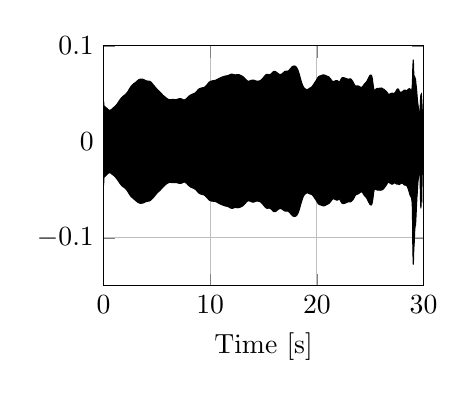
\begin{tikzpicture}

\begin{axis}[%
width=1.6in,
height=1.2in,
at={(0.758in,0.481in)},
scale only axis,
xmin=0,
xmax=30,
xmajorgrids,
ymin=-0.15,
ymax=0.1,
ymajorgrids,
xlabel={Time [s]},
axis background/.style={fill=white}
]
\addplot[fill=black,draw=black,forget plot] plot table[row sep=crcr]{%
2.08333333333333e-05	0.0422468185424805\\
0.0417454218822439	0.0372525453567505\\
0.0834700104311544	0.0369192361831665\\
0.125194598980065	0.0365363359451294\\
0.166919187528975	0.0361708402633667\\
0.208643776077886	0.0357952117919922\\
0.250368364626797	0.0354363918304443\\
0.292092953175707	0.0350120067596436\\
0.333817541724618	0.0345685482025146\\
0.375542130273528	0.0340954065322876\\
0.417266718822439	0.033664345741272\\
0.458991307371349	0.033263087272644\\
0.50071589592026	0.0329965353012085\\
0.54244048446917	0.0328166484832764\\
0.584165073018081	0.0327619314193726\\
0.625889661566991	0.0329329967498779\\
0.667614250115902	0.0331350564956665\\
0.709338838664812	0.0334482192993164\\
0.751063427213723	0.0337620973587036\\
0.792788015762633	0.03410804271698\\
0.834512604311544	0.0344952344894409\\
0.876237192860454	0.0349040031433105\\
0.917961781409365	0.0353187322616577\\
0.959686369958275	0.0357452630996704\\
1.00141095850719	0.0361156463623047\\
1.0431355470561	0.0365282297134399\\
1.08486013560501	0.0369502305984497\\
1.12658472415392	0.037433385848999\\
1.16830931270283	0.0379418134689331\\
1.21003390125174	0.0385125875473022\\
1.25175848980065	0.0390442609786987\\
1.29348307834956	0.0396722555160522\\
1.33520766689847	0.0403273105621338\\
1.37693225544738	0.0410159826278687\\
1.41865684399629	0.0416945219039917\\
1.4603814325452	0.0424588918685913\\
1.50210602109411	0.0431810617446899\\
1.54383060964302	0.0438424348831177\\
1.58555519819193	0.0444444417953491\\
1.62727978674084	0.0450773239135742\\
1.66900437528975	0.0456510782241821\\
1.71072896383866	0.0461443662643433\\
1.75245355238758	0.0466166734695435\\
1.79417814093649	0.0470112562179565\\
1.8359027294854	0.0473984479904175\\
1.87762731803431	0.0477943420410156\\
1.91935190658322	0.0481898784637451\\
1.96107649513213	0.0485495328903198\\
2.00280108368104	0.048880934715271\\
2.04452567222995	0.0492501258850098\\
2.08625026077886	0.049651026725769\\
2.12797484932777	0.0502268075942993\\
2.16969943787668	0.0507606267929077\\
2.21142402642559	0.0513180494308472\\
2.2531486149745	0.0518807172775269\\
2.29487320352341	0.0525689125061035\\
2.33659779207232	0.0533157587051392\\
2.37832238062123	0.0541360378265381\\
2.42004696917014	0.054889440536499\\
2.46177155771905	0.0557056665420532\\
2.50349614626796	0.0564498901367188\\
2.54522073481687	0.0571705102920532\\
2.58694532336579	0.0578427314758301\\
2.6286699119147	0.0584187507629395\\
2.67039450046361	0.0589123964309692\\
2.71211908901252	0.0591186285018921\\
2.75384367756143	0.0597426891326904\\
2.79556826611034	0.0601574182510376\\
2.83729285465925	0.0605597496032715\\
2.87901744320816	0.0608901977539063\\
2.92074203175707	0.061190128326416\\
2.96246662030598	0.0615092515945435\\
3.00419120885489	0.0618681907653809\\
3.0459157974038	0.0622962713241577\\
3.08764038595271	0.0627272129058838\\
3.12936497450162	0.063151478767395\\
3.17108956305053	0.0635229349136353\\
3.21281415159944	0.0639200210571289\\
3.25453874014835	0.0642675161361694\\
3.29626332869726	0.0646072626113892\\
3.33798791724618	0.064887523651123\\
3.37971250579509	0.0650652647018433\\
3.421437094344	0.0651521682739258\\
3.46316168289291	0.0652352571487427\\
3.50488627144182	0.0652922391891479\\
3.54661085999073	0.0653144121170044\\
3.58833544853964	0.0652894973754883\\
3.63006003708855	0.0652514696121216\\
3.67178462563746	0.065137505531311\\
3.71350921418637	0.0650078058242798\\
3.75523380273528	0.0648300647735596\\
3.79695839128419	0.0646129846572876\\
3.8386829798331	0.0644136667251587\\
3.88040756838201	0.0641599893569946\\
3.92213215693092	0.0637109279632568\\
3.96385674547983	0.0636776685714722\\
4.00558133402874	0.0635045766830444\\
4.04730592257765	0.0633904933929443\\
4.08903051112656	0.0633418560028076\\
4.13075509967547	0.063257098197937\\
4.17247968822439	0.0632200241088867\\
4.2142042767733	0.063180685043335\\
4.25592886532221	0.0631259679794312\\
4.29765345387112	0.0630643367767334\\
4.33937804242003	0.062917947769165\\
4.38110263096894	0.0626916885375977\\
4.42282721951785	0.06235671043396\\
4.46455180806676	0.0618894100189209\\
4.50627639661567	0.0613611936569214\\
4.54800098516458	0.0608628988265991\\
4.58972557371349	0.0602775812149048\\
4.6314501622624	0.0597318410873413\\
4.67317475081131	0.0591355562210083\\
4.71489933936022	0.0585864782333374\\
4.75662392790913	0.0580800771713257\\
4.79834851645804	0.0575709342956543\\
4.84007310500695	0.0570741891860962\\
4.88179769355586	0.0565125942230225\\
4.92352228210478	0.0559226274490356\\
4.96524687065368	0.055355429649353\\
5.0069714592026	0.05479896068573\\
5.04869604775151	0.054322361946106\\
5.09042063630042	0.0538897514343262\\
5.13214522484933	0.053453803062439\\
5.17386981339824	0.0530737638473511\\
5.21559440194715	0.052641749382019\\
5.25731899049606	0.0521992444992065\\
5.29904357904497	0.051758885383606\\
5.34076816759388	0.0512574911117554\\
5.38249275614279	0.0507074594497681\\
5.4242173446917	0.0502089262008667\\
5.46594193324061	0.0497028827667236\\
5.50766652178952	0.0491554737091064\\
5.54939111033843	0.0486928224563599\\
5.59111569888734	0.0482624769210815\\
5.63284028743625	0.047857403755188\\
5.67456487598516	0.047433614730835\\
5.71628946453407	0.0470389127731323\\
5.75801405308299	0.0466983318328857\\
5.7997386416319	0.046233057975769\\
5.84146323018081	0.045886754989624\\
5.88318781872972	0.0455105304718018\\
5.92491240727863	0.045197606086731\\
5.96663699582754	0.0449239015579224\\
6.00836158437645	0.0446234941482544\\
6.05008617292536	0.0442850589752197\\
6.09181076147427	0.0440802574157715\\
6.13353535002318	0.0438753366470337\\
6.17525993857209	0.0437972545623779\\
6.216984527121	0.0438199043273926\\
6.25870911566991	0.0438779592514038\\
6.30043370421882	0.0439367294311523\\
6.34215829276773	0.0439809560775757\\
6.38388288131664	0.0440677404403687\\
6.42560746986555	0.0441368818283081\\
6.46733205841446	0.0441353321075439\\
6.50905664696338	0.0441091060638428\\
6.55078123551229	0.0440609455108643\\
6.5925058240612	0.043999195098877\\
6.63423041261011	0.0439372062683105\\
6.67595500115902	0.0439157485961914\\
6.71767958970793	0.0439170598983765\\
6.75940417825684	0.043918251991272\\
6.80112876680575	0.0439597368240356\\
6.84285335535466	0.0440601110458374\\
6.88457794390357	0.0441927909851074\\
6.92630253245248	0.0443743467330933\\
6.96802712100139	0.0444844961166382\\
7.0097517095503	0.0445874929428101\\
7.05147629809921	0.0447444915771484\\
7.09320088664812	0.0448503494262695\\
7.13492547519703	0.0449130535125732\\
7.17665006374594	0.0449339151382446\\
7.21837465229485	0.044910192489624\\
7.26009924084376	0.0448141098022461\\
7.30182382939268	0.0446615219116211\\
7.34354841794159	0.0444469451904297\\
7.3852730064905	0.0441970825195313\\
7.42699759503941	0.0439774990081787\\
7.46872218358832	0.0437713861465454\\
7.51044677213723	0.0436021089553833\\
7.55217136068614	0.0435445308685303\\
7.59389594923505	0.0436593294143677\\
7.63562053778396	0.043853759765625\\
7.67734512633287	0.0441319942474365\\
7.71906971488178	0.0444629192352295\\
7.76079430343069	0.0447800159454346\\
7.8025188919796	0.0453106164932251\\
7.84424348052851	0.0457882881164551\\
7.88596806907742	0.0462902784347534\\
7.92769265762633	0.0467329025268555\\
7.96941724617524	0.0471514463424683\\
8.01114183472416	0.0475220680236816\\
8.05286642327307	0.047889232635498\\
8.09459101182198	0.0482308864593506\\
8.13631560037089	0.0485328435897827\\
8.1780401889198	0.048784613609314\\
8.21976477746871	0.0490474700927734\\
8.26148936601762	0.0492734909057617\\
8.30321395456653	0.0494829416275024\\
8.34493854311544	0.0496753454208374\\
8.38666313166435	0.0498688220977783\\
8.42838772021326	0.0500140190124512\\
8.47011230876217	0.0501646995544434\\
8.51183689731108	0.0504004955291748\\
8.55356148585999	0.0506466627120972\\
8.5952860744089	0.0510271787643433\\
8.63701066295781	0.0513583421707153\\
8.67873525150672	0.0517593622207642\\
8.72045984005563	0.0522468090057373\\
8.76218442860454	0.0528092384338379\\
8.80390901715345	0.0533682107925415\\
8.84563360570237	0.053951621055603\\
8.88735819425128	0.0544096231460571\\
8.92908278280018	0.0548523664474487\\
8.9708073713491	0.0551828145980835\\
9.01253195989801	0.0554293394088745\\
9.05425654844692	0.0556589365005493\\
9.09598113699583	0.0558258295059204\\
9.13770572554474	0.0559313297271729\\
9.17943031409365	0.0560096502304077\\
9.22115490264256	0.0561132431030273\\
9.26287949119147	0.0562242269515991\\
9.30460407974038	0.0563126802444458\\
9.34632866828929	0.0564223527908325\\
9.3880532568382	0.0564727783203125\\
9.42977784538711	0.0566496849060059\\
9.47150243393602	0.0569214820861816\\
9.51322702248493	0.0572543144226074\\
9.55495161103384	0.057722806930542\\
9.59667619958275	0.0581281185150146\\
9.63840078813166	0.058588981628418\\
9.68012537668058	0.0590826272964478\\
9.72184996522949	0.0596930980682373\\
9.7635745537784	0.0602951049804688\\
9.80529914232731	0.0608705282211304\\
9.84702373087622	0.0613894462585449\\
9.88874831942513	0.0618714094161987\\
9.93047290797404	0.0622662305831909\\
9.97219749652295	0.0625808238983154\\
10.0139220850719	0.0628762245178223\\
10.0556466736208	0.0630688667297363\\
10.0973712621697	0.0631923675537109\\
10.1390958507186	0.0633230209350586\\
10.1808204392675	0.0634113550186157\\
10.2225450278164	0.0635578632354736\\
10.2642696163653	0.0636551380157471\\
10.3059942049142	0.06374192237854\\
10.3477187934631	0.0638207197189331\\
10.3894433820121	0.0638954639434814\\
10.431167970561	0.0639438629150391\\
10.4728925591099	0.0640406608581543\\
10.5146171476588	0.0641665458679199\\
10.5563417362077	0.064362645149231\\
10.5980663247566	0.0645772218704224\\
10.6397909133055	0.0648475885391235\\
10.6815155018544	0.0650749206542969\\
10.7232400904033	0.0653728246688843\\
10.7649646789523	0.0656516551971436\\
10.8066892675012	0.0658563375473022\\
10.8484138560501	0.06606125831604\\
10.890138444599	0.0663137435913086\\
10.9318630331479	0.0665462017059326\\
10.9735876216968	0.0667338371276855\\
11.0153122102457	0.066963791847229\\
11.0570367987946	0.0671656131744385\\
11.0987613873435	0.0673573017120361\\
11.1404859758924	0.0675303936004639\\
11.1822105644414	0.0676944255828857\\
11.2239351529903	0.0678578615188599\\
11.2656597415392	0.067983865737915\\
11.3073843300881	0.068114161491394\\
11.349108918637	0.0682580471038818\\
11.3908335071859	0.0683811902999878\\
11.4325580957348	0.0685162544250488\\
11.4742826842837	0.0686306953430176\\
11.5160072728326	0.0686953067779541\\
11.5577318613816	0.0687469244003296\\
11.5994564499305	0.0688079595565796\\
11.6411810384794	0.0689411163330078\\
11.6829056270283	0.0690766572952271\\
11.7246302155772	0.0692694187164307\\
11.7663548041261	0.0694770812988281\\
11.808079392675	0.0697073936462402\\
11.8498039812239	0.0699185132980347\\
11.8915285697728	0.0701367855072021\\
11.9332531583217	0.0703275203704834\\
11.9749777468707	0.0704201459884644\\
12.0167023354196	0.070447564125061\\
12.0584269239685	0.0704313516616821\\
12.1001515125174	0.070331335067749\\
12.1418761010663	0.0702515840530396\\
12.1836006896152	0.0700995922088623\\
12.2253252781641	0.0699683427810669\\
12.267049866713	0.0698189735412598\\
12.3087744552619	0.0697275400161743\\
12.3504990438108	0.0696953535079956\\
12.3922236323598	0.0697113275527954\\
12.4339482209087	0.0698176622390747\\
12.4756728094576	0.0698702335357666\\
12.5173973980065	0.0699410438537598\\
12.5591219865554	0.0699845552444458\\
12.6008465751043	0.0699983835220337\\
12.6425711636532	0.0699825286865234\\
12.6842957522021	0.0699266195297241\\
12.726020340751	0.0698097944259644\\
12.7677449293	0.0696190595626831\\
12.8094695178489	0.0693641901016235\\
12.8511941063978	0.0691491365432739\\
12.8929186949467	0.0689480304718018\\
12.9346432834956	0.0687199831008911\\
12.9763678720445	0.0684479475021362\\
13.0180924605934	0.0681353807449341\\
13.0598170491423	0.0678220987319946\\
13.1015416376912	0.0674749612808228\\
13.1432662262401	0.0670442581176758\\
13.1849908147891	0.0666248798370361\\
13.226715403338	0.0661572217941284\\
13.2684399918869	0.0656723976135254\\
13.3101645804358	0.0651500225067139\\
13.3518891689847	0.06462562084198\\
13.3936137575336	0.0642530918121338\\
13.4353383460825	0.0638662576675415\\
13.4770629346314	0.0635504722595215\\
13.5187875231803	0.0633330345153809\\
13.5605121117293	0.0631518363952637\\
13.6022367002782	0.0631347894668579\\
13.6439612888271	0.0632275342941284\\
13.685685877376	0.0633029937744141\\
13.7274104659249	0.0634669065475464\\
13.7691350544738	0.0636700391769409\\
13.8108596430227	0.0638896226882935\\
13.8525842315716	0.064056396484375\\
13.8943088201205	0.0642024278640747\\
13.9360334086694	0.0642625093460083\\
13.9777579972184	0.0643131732940674\\
14.0194825857673	0.0643172264099121\\
14.0612071743162	0.0642516613006592\\
14.1029317628651	0.0641590356826782\\
14.144656351414	0.0639668703079224\\
14.1863809399629	0.0637030601501465\\
14.2281055285118	0.0635595321655273\\
14.2698301170607	0.0633617639541626\\
14.3115547056096	0.0632978677749634\\
14.3532792941586	0.063257098197937\\
14.3950038827075	0.0632302761077881\\
14.4367284712564	0.0631743669509888\\
14.4784530598053	0.0631651878356934\\
14.5201776483542	0.0631885528564453\\
14.5619022369031	0.0632354021072388\\
14.603626825452	0.0633671283721924\\
14.6453514140009	0.0635287761688232\\
14.6870760025498	0.0637497901916504\\
14.7288005910988	0.0640381574630737\\
14.7705251796477	0.0643914937973022\\
14.8122497681966	0.0647845268249512\\
14.8539743567455	0.0652201175689697\\
14.8956989452944	0.0657086372375488\\
14.9374235338433	0.0661934614181519\\
14.9791481223922	0.0667743682861328\\
15.0208727109411	0.0673575401306152\\
15.06259729949	0.0678131580352783\\
15.1043218880389	0.0684419870376587\\
15.1460464765879	0.0689877271652222\\
15.1877710651368	0.0694783926010132\\
15.2294956536857	0.0698593854904175\\
15.2712202422346	0.0701580047607422\\
15.3129448307835	0.0702724456787109\\
15.3546694193324	0.0702666044235229\\
15.3963940078813	0.0702189207077026\\
15.4381185964302	0.0700663328170776\\
15.4798431849791	0.0699518918991089\\
15.521567773528	0.0698869228363037\\
15.563292362077	0.069893479347229\\
15.6050169506259	0.0700204372406006\\
15.6467415391748	0.0702553987503052\\
15.6884661277237	0.0705602169036865\\
15.7301907162726	0.0709625482559204\\
15.7719153048215	0.0713804960250854\\
15.8136398933704	0.0719301700592041\\
15.8553644819193	0.0724350214004517\\
15.8970890704682	0.0728191137313843\\
15.9388136590172	0.0730979442596436\\
15.9805382475661	0.0732845067977905\\
16.022262836115	0.0733399391174316\\
16.0639874246639	0.0733081102371216\\
16.1057120132128	0.07317054271698\\
16.1474366017617	0.0728867053985596\\
16.1891611903106	0.0726271867752075\\
16.2308857788595	0.072283148765564\\
16.2726103674084	0.0719183683395386\\
16.3143349559573	0.0715353488922119\\
16.3560595445063	0.0711410045623779\\
16.3977841330552	0.070814847946167\\
16.4395087216041	0.0704998970031738\\
16.481233310153	0.0703115463256836\\
16.5229578987019	0.0701476335525513\\
16.5646824872508	0.0700541734695435\\
16.6064070757997	0.0700763463973999\\
16.6481316643486	0.0702290534973145\\
16.6898562528975	0.0704755783081055\\
16.7315808414465	0.0708328485488892\\
16.7733054299954	0.0711541175842285\\
16.8150300185443	0.0715680122375488\\
16.8567546070932	0.0720105171203613\\
16.8984791956421	0.0724157094955444\\
16.940203784191	0.0728104114532471\\
16.9819283727399	0.0731693506240845\\
17.0236529612888	0.0733708143234253\\
17.0653775498377	0.0734338760375977\\
17.1071021383867	0.0734831094741821\\
17.1488267269356	0.0734776258468628\\
17.1905513154845	0.0734367370605469\\
17.2322759040334	0.0735143423080444\\
17.2740004925823	0.073606014251709\\
17.3157250811312	0.0738447904586792\\
17.3574496696801	0.0742049217224121\\
17.399174258229	0.074642539024353\\
17.4408988467779	0.0750911235809326\\
17.4826234353268	0.075647234916687\\
17.5243480238758	0.0761734247207642\\
17.5660726124247	0.0766944885253906\\
17.6077972009736	0.0772606134414673\\
17.6495217895225	0.0777366161346436\\
17.6912463780714	0.0782027244567871\\
17.7329709666203	0.0785583257675171\\
17.7746955551692	0.0787789821624756\\
17.8164201437181	0.0789024829864502\\
17.858144732267	0.0789288282394409\\
17.8998693208159	0.0789124965667725\\
17.9415939093649	0.0788314342498779\\
17.9833184979138	0.0786029100418091\\
18.0250430864627	0.078234076499939\\
18.0667676750116	0.0777355432510376\\
18.1084922635605	0.077067494392395\\
18.1502168521094	0.0763176679611206\\
18.1919414406583	0.0752838850021362\\
18.2336660292072	0.0741901397705078\\
18.2753906177561	0.0728087425231934\\
18.3171152063051	0.0713739395141602\\
18.358839794854	0.0698267221450806\\
18.4005643834029	0.0681694746017456\\
18.4422889719518	0.0664654970169067\\
18.4840135605007	0.0648053884506226\\
18.5257381490496	0.0631289482116699\\
18.5674627375985	0.061661958694458\\
18.6091873261474	0.0603326559066772\\
18.6509119146963	0.0591540336608887\\
18.6926365032453	0.0580891370773315\\
18.7343610917942	0.0571942329406738\\
18.7760856803431	0.0564507246017456\\
18.817810268892	0.0559170246124268\\
18.8595348574409	0.055516242980957\\
18.9012594459898	0.0551298856735229\\
18.9429840345387	0.0548285245895386\\
18.9847086230876	0.0545656681060791\\
19.0264332116365	0.0544030666351318\\
19.0681578001854	0.0543440580368042\\
19.1098823887344	0.0544142723083496\\
19.1516069772833	0.0546382665634155\\
19.1933315658322	0.0548405647277832\\
19.2350561543811	0.0551340579986572\\
19.27678074293	0.0554288625717163\\
19.3185053314789	0.0557364225387573\\
19.3602299200278	0.0560226440429688\\
19.4019545085767	0.0562071800231934\\
19.4436790971256	0.0564566850662231\\
19.4854036856745	0.0567950010299683\\
19.5271282742235	0.0572218894958496\\
19.5688528627724	0.0578150749206543\\
19.6105774513213	0.0584547519683838\\
19.6523020398702	0.0591301918029785\\
19.6940266284191	0.059847354888916\\
19.735751216968	0.0605363845825195\\
19.7774758055169	0.0612852573394775\\
19.8192003940658	0.0619161128997803\\
19.8609249826147	0.0625683069229126\\
19.9026495711637	0.0632625818252563\\
19.9443741597126	0.0639643669128418\\
19.9860987482615	0.0647803544998169\\
20.0278233368104	0.0656101703643799\\
20.0695479253593	0.0664572715759277\\
20.1112725139082	0.0671699047088623\\
20.1529971024571	0.067791223526001\\
20.194721691006	0.068149209022522\\
20.2364462795549	0.0683226585388184\\
20.2781708681038	0.0685330629348755\\
20.3198954566528	0.0686384439468384\\
20.3616200452017	0.0687670707702637\\
20.4033446337506	0.0689530372619629\\
20.4450692222995	0.0691442489624023\\
20.4867938108484	0.0693328380584717\\
20.5285183993973	0.0695230960845947\\
20.5702429879462	0.0696732997894287\\
20.6119675764951	0.069696307182312\\
20.653692165044	0.0696195363998413\\
20.695416753593	0.0695405006408691\\
20.7371413421419	0.0694179534912109\\
20.7788659306908	0.0692507028579712\\
20.8205905192397	0.0690499544143677\\
20.8623151077886	0.0688378810882568\\
20.9040396963375	0.0685629844665527\\
20.9457642848864	0.0683460235595703\\
20.9874888734353	0.0681912899017334\\
21.0292134619842	0.0680167675018311\\
21.0709380505331	0.0678391456604004\\
21.1126626390821	0.0675274133682251\\
21.154387227631	0.067095160484314\\
21.1961118161799	0.0665644407272339\\
21.2378364047288	0.0659773349761963\\
21.2795609932777	0.0654546022415161\\
21.3212855818266	0.0648322105407715\\
21.3630101703755	0.0641556978225708\\
21.4047347589244	0.06363844871521\\
21.4464593474733	0.0631991624832153\\
21.4881839360223	0.0629258155822754\\
21.5299085245712	0.0627888441085815\\
21.5716331131201	0.0627902746200562\\
21.613357701669	0.0629123449325562\\
21.6550822902179	0.0631364583969116\\
21.6968068787668	0.0633445978164673\\
21.7385314673157	0.0635623931884766\\
21.7802560558646	0.0636688470840454\\
21.8219806444135	0.063738226890564\\
21.8637052329624	0.0637307167053223\\
21.9054298215114	0.0636621713638306\\
21.9471544100603	0.0634632110595703\\
21.9888789986092	0.0631618499755859\\
22.0306035871581	0.0625883340835571\\
22.072328175707	0.0620317459106445\\
22.1140527642559	0.0619052648544312\\
22.1557773528048	0.062762975692749\\
22.1975019413537	0.0638045072555542\\
22.2392265299026	0.0646953582763672\\
22.2809511184516	0.0655143260955811\\
22.3226757070005	0.0660974979400635\\
22.3644002955494	0.0665786266326904\\
22.4061248840983	0.0667860507965088\\
22.4478494726472	0.0669149160385132\\
22.4895740611961	0.0668758153915405\\
22.531298649745	0.066770076751709\\
22.5730232382939	0.0665502548217773\\
22.6147478268428	0.0664300918579102\\
22.6564724153917	0.0662775039672852\\
22.6981970039407	0.0660278797149658\\
22.7399215924896	0.0659236907958984\\
22.7816461810385	0.0657963752746582\\
22.8233707695874	0.0656427145004272\\
22.8650953581363	0.065447211265564\\
22.9068199466852	0.0652456283569336\\
22.9485445352341	0.0652828216552734\\
22.990269123783	0.0652694702148438\\
23.0319937123319	0.0654103755950928\\
23.0737183008809	0.0654884576797485\\
23.1154428894298	0.0655225515365601\\
23.1571674779787	0.0654964447021484\\
23.1988920665276	0.0651679039001465\\
23.2406166550765	0.0648037195205688\\
23.2823412436254	0.0640715360641479\\
23.3240658321743	0.0634130239486694\\
23.3657904207232	0.0626559257507324\\
23.4075150092721	0.0619316101074219\\
23.449239597821	0.0610703229904175\\
23.49096418637	0.0601691007614136\\
23.5326887749189	0.0592845678329468\\
23.5744133634678	0.0585769414901733\\
23.6161379520167	0.0581790208816528\\
23.6578625405656	0.0580800771713257\\
23.6995871291145	0.0580724477767944\\
23.7413117176634	0.0581483840942383\\
23.7830363062123	0.0581809282302856\\
23.8247608947612	0.0581555366516113\\
23.8664854833102	0.0581238269805908\\
23.9082100718591	0.0580016374588013\\
23.949934660408	0.0578075647354126\\
23.9916592489569	0.0575815439224243\\
24.0333838375058	0.0572960376739502\\
24.0751084260547	0.0569047927856445\\
24.1168330146036	0.0566414594650269\\
24.1585576031525	0.0566698312759399\\
24.2002821917014	0.0568233728408813\\
24.2420067802503	0.0571283102035522\\
24.2837313687993	0.0575376749038696\\
24.3254559573482	0.0581129789352417\\
24.3671805458971	0.0587639808654785\\
24.408905134446	0.0594481229782104\\
24.4506297229949	0.0600841045379639\\
24.4923543115438	0.0606585741043091\\
24.5340789000927	0.0611315965652466\\
24.5758034886416	0.0615746974945068\\
24.6175280771905	0.0620625019073486\\
24.6592526657395	0.0626002550125122\\
24.7009772542884	0.0633838176727295\\
24.7427018428373	0.0642297267913818\\
24.7844264313862	0.0651358366012573\\
24.8261510199351	0.0660654306411743\\
24.867875608484	0.0670012235641479\\
24.9096001970329	0.0678833723068237\\
24.9513247855818	0.0687386989593506\\
24.9930493741307	0.0693345069885254\\
25.0347739626796	0.0693637132644653\\
25.0764985512286	0.0694910287857056\\
25.1182231397775	0.0689376592636108\\
25.1599477283264	0.067712664604187\\
25.2016723168753	0.0654442310333252\\
25.2433969054242	0.0616657733917236\\
25.2851214939731	0.058199405670166\\
25.326846082522	0.0554147958755493\\
25.3685706710709	0.0537508726119995\\
25.4102952596198	0.0532442331314087\\
25.4520198481687	0.0534800291061401\\
25.4937444367177	0.054113507270813\\
25.5354690252666	0.0547759532928467\\
25.5771936138155	0.0551197528839111\\
25.6189182023644	0.0553914308547974\\
25.6606427909133	0.0555583238601685\\
25.7023673794622	0.0556082725524902\\
25.7440919680111	0.0553638935089111\\
25.78581655656	0.0555232763290405\\
25.8275411451089	0.0555715560913086\\
25.8692657336579	0.0557857751846313\\
25.9109903222068	0.0558958053588867\\
25.9527149107557	0.0559850931167603\\
25.9944394993046	0.0559875965118408\\
26.0361640878535	0.0560027360916138\\
26.0778886764024	0.0558562278747559\\
26.1196132649513	0.05565345287323\\
26.1613378535002	0.0553421974182129\\
26.2030624420491	0.0550359487533569\\
26.2447870305981	0.054937481880188\\
26.286511619147	0.0546416044235229\\
26.3282362076959	0.0542027950286865\\
26.3699607962448	0.0537012815475464\\
26.4116853847937	0.0534621477127075\\
26.4534099733426	0.0530197620391846\\
26.4951345618915	0.0525045394897461\\
26.5368591504404	0.0520088672637939\\
26.5785837389893	0.0515090227127075\\
26.6203083275383	0.0509911775588989\\
26.6620329160872	0.0501706600189209\\
26.7037575046361	0.049569845199585\\
26.745482093185	0.0492426156997681\\
26.7872066817339	0.049281120300293\\
26.8289312702828	0.0496653318405151\\
26.8706558588317	0.0500508546829224\\
26.9123804473806	0.0502486228942871\\
26.9541050359295	0.0504103899002075\\
26.9958296244784	0.0505565404891968\\
27.0375542130274	0.0507067441940308\\
27.0792788015763	0.0507726669311523\\
27.1210033901252	0.0506423711776733\\
27.1627279786741	0.0503650903701782\\
27.204452567223	0.050268292427063\\
27.2461771557719	0.0503370761871338\\
27.2879017443208	0.0508761405944824\\
27.3296263328697	0.0511735677719116\\
27.3713509214186	0.0513689517974854\\
27.4130755099675	0.0527089834213257\\
27.4548000985165	0.0535047054290771\\
27.4965246870654	0.0542939901351929\\
27.5382492756143	0.054874062538147\\
27.5799738641632	0.0550172328948975\\
27.6216984527121	0.0549682378768921\\
27.663423041261	0.054347038269043\\
27.7051476298099	0.0530894994735718\\
27.7468722183588	0.0522401332855225\\
27.7885968069077	0.0516880750656128\\
27.8303213954567	0.0517263412475586\\
27.8720459840056	0.0517513751983643\\
27.9137705725545	0.0517706871032715\\
27.9554951611034	0.0516763925552368\\
27.9972197496523	0.0521132946014404\\
28.0389443382012	0.052584171295166\\
28.0806689267501	0.0528182983398438\\
28.122393515299	0.0531265735626221\\
28.1641181038479	0.0536978244781494\\
28.2058426923968	0.0538284778594971\\
28.2475672809458	0.0538012981414795\\
28.2892918694947	0.0536890029907227\\
28.3310164580436	0.0533449649810791\\
28.3727410465925	0.0531834363937378\\
28.4144656351414	0.053068995475769\\
28.4561902236903	0.0532664060592651\\
28.4979148122392	0.0538042783737183\\
28.5396394007881	0.0544805526733398\\
28.581363989337	0.0548857450485229\\
28.623088577886	0.0551347732543945\\
28.6648131664349	0.0552659034729004\\
28.7065377549838	0.0551073551177979\\
28.7482623435327	0.0548173189163208\\
28.7899869320816	0.0539336204528809\\
28.8317115206305	0.0526777505874634\\
28.8734361091794	0.0522592067718506\\
28.9151606977283	0.0549857616424561\\
28.9568852862772	0.0610247850418091\\
28.9986098748261	0.0790016651153564\\
29.0403344633751	0.0856187343597412\\
29.082059051924	0.0708431005477905\\
29.1237836404729	0.066988468170166\\
29.1655082290218	0.0639430284500122\\
29.2072328175707	0.0662022829055786\\
29.2489574061196	0.0648359060287476\\
29.2906819946685	0.0598307847976685\\
29.3324065832174	0.056273341178894\\
29.3741311717663	0.0502718687057495\\
29.4158557603153	0.0443309545516968\\
29.4575803488642	0.0401654243469238\\
29.4993049374131	0.0367835760116577\\
29.541029525962	0.0328407287597656\\
29.5827541145109	0.0275323390960693\\
29.6244787030598	0.0247510671615601\\
29.6662032916087	0.0281398296356201\\
29.7079278801576	0.0431309938430786\\
29.7496524687065	0.0489364862442017\\
29.7913770572554	0.0496424436569214\\
29.8331016458044	0.0429533720016479\\
29.8748262343533	0.0333377122879028\\
29.9165508229022	0.0223888158798218\\
29.9582754114511	0.0127576589584351\\
30	0.0128462314605713\\
}
\closedcycle;
\addplot[fill=black,draw=black,forget plot] plot table[row sep=crcr]{%
2.08333333333333e-05	-0.0452835559844971\\
0.0417454218822439	-0.0365959405899048\\
0.0834700104311544	-0.0363312959671021\\
0.125194598980065	-0.0360137224197388\\
0.166919187528975	-0.0356215238571167\\
0.208643776077886	-0.0351780652999878\\
0.250368364626797	-0.0347000360488892\\
0.292092953175707	-0.0342026948928833\\
0.333817541724618	-0.0337598323822021\\
0.375542130273528	-0.0333238840103149\\
0.417266718822439	-0.0328874588012695\\
0.458991307371349	-0.0325144529342651\\
0.50071589592026	-0.0322558879852295\\
0.54244048446917	-0.0321190357208252\\
0.584165073018081	-0.0322035551071167\\
0.625889661566991	-0.032343864440918\\
0.667614250115902	-0.0325241088867188\\
0.709338838664812	-0.0328241586685181\\
0.751063427213723	-0.0331873893737793\\
0.792788015762633	-0.0335942506790161\\
0.834512604311544	-0.0339881181716919\\
0.876237192860454	-0.0343648195266724\\
0.917961781409365	-0.0347262620925903\\
0.959686369958275	-0.0350478887557983\\
1.00141095850719	-0.0354864597320557\\
1.0431355470561	-0.0359150171279907\\
1.08486013560501	-0.0364131927490234\\
1.12658472415392	-0.0368940830230713\\
1.16830931270283	-0.0374562740325928\\
1.21003390125174	-0.0380069017410278\\
1.25175848980065	-0.038679838180542\\
1.29348307834956	-0.0392719507217407\\
1.33520766689847	-0.0399441719055176\\
1.37693225544738	-0.0405129194259644\\
1.41865684399629	-0.0411608219146729\\
1.4603814325452	-0.0420024394989014\\
1.50210602109411	-0.0427336692810059\\
1.54383060964302	-0.0433487892150879\\
1.58555519819193	-0.0439862012863159\\
1.62727978674084	-0.0445595979690552\\
1.66900437528975	-0.0450965166091919\\
1.71072896383866	-0.0456123352050781\\
1.75245355238758	-0.0460573434829712\\
1.79417814093649	-0.0464980602264404\\
1.8359027294854	-0.0467829704284668\\
1.87762731803431	-0.0470947027206421\\
1.91935190658322	-0.0474388599395752\\
1.96107649513213	-0.0477988719940186\\
2.00280108368104	-0.0481970310211182\\
2.04452567222995	-0.0485557317733765\\
2.08625026077886	-0.0489752292633057\\
2.12797484932777	-0.0495154857635498\\
2.16969943787668	-0.0500869750976563\\
2.21142402642559	-0.0507384538650513\\
2.2531486149745	-0.0514688491821289\\
2.29487320352341	-0.0521427392959595\\
2.33659779207232	-0.0528820753097534\\
2.37832238062123	-0.053626537322998\\
2.42004696917014	-0.0544383525848389\\
2.46177155771905	-0.0551594495773315\\
2.50349614626796	-0.0558806657791138\\
2.54522073481687	-0.0564572811126709\\
2.58694532336579	-0.0569438934326172\\
2.6286699119147	-0.057425856590271\\
2.67039450046361	-0.057841420173645\\
2.71211908901252	-0.0581755638122559\\
2.75384367756143	-0.0586920976638794\\
2.79556826611034	-0.0591189861297607\\
2.83729285465925	-0.0594843626022339\\
2.87901744320816	-0.059850811958313\\
2.92074203175707	-0.0602942705154419\\
2.96246662030598	-0.0606968402862549\\
3.00419120885489	-0.0611178874969482\\
3.0459157974038	-0.061500072479248\\
3.08764038595271	-0.0618867874145508\\
3.12936497450162	-0.0622377395629883\\
3.17108956305053	-0.0626332759857178\\
3.21281415159944	-0.0629510879516602\\
3.25453874014835	-0.0632561445236206\\
3.29626332869726	-0.0634527206420898\\
3.33798791724618	-0.0636600255966187\\
3.37971250579509	-0.0638314485549927\\
3.421437094344	-0.0639530420303345\\
3.46316168289291	-0.0640033483505249\\
3.50488627144182	-0.0640106201171875\\
3.54661085999073	-0.0639750957489014\\
3.58833544853964	-0.0638896226882935\\
3.63006003708855	-0.0638022422790527\\
3.67178462563746	-0.0637279748916626\\
3.71350921418637	-0.0636403560638428\\
3.75523380273528	-0.0634739398956299\\
3.79695839128419	-0.0632733106613159\\
3.8386829798331	-0.0630378723144531\\
3.88040756838201	-0.062753438949585\\
3.92213215693092	-0.0625588893890381\\
3.96385674547983	-0.0623416900634766\\
4.00558133402874	-0.0621813535690308\\
4.04730592257765	-0.0620478391647339\\
4.08903051112656	-0.06192946434021\\
4.13075509967547	-0.0618768930435181\\
4.17247968822439	-0.0618360042572021\\
4.2142042767733	-0.0618084669113159\\
4.25592886532221	-0.0616815090179443\\
4.29765345387112	-0.061535120010376\\
4.33937804242003	-0.0613168478012085\\
4.38110263096894	-0.0610744953155518\\
4.42282721951785	-0.0607260465621948\\
4.46455180806676	-0.0603333711624146\\
4.50627639661567	-0.0597552061080933\\
4.54800098516458	-0.0593008995056152\\
4.58972557371349	-0.058842658996582\\
4.6314501622624	-0.0583441257476807\\
4.67317475081131	-0.0578821897506714\\
4.71489933936022	-0.0573632717132568\\
4.75662392790913	-0.0568132400512695\\
4.79834851645804	-0.0561885833740234\\
4.84007310500695	-0.0556766986846924\\
4.88179769355586	-0.0551367998123169\\
4.92352228210478	-0.0545719861984253\\
4.96524687065368	-0.0539889335632324\\
5.0069714592026	-0.053318977355957\\
5.04869604775151	-0.052852988243103\\
5.09042063630042	-0.0524715185165405\\
5.13214522484933	-0.0520952939987183\\
5.17386981339824	-0.0517055988311768\\
5.21559440194715	-0.0512887239456177\\
5.25731899049606	-0.0508548021316528\\
5.29904357904497	-0.0503756999969482\\
5.34076816759388	-0.0498943328857422\\
5.38249275614279	-0.0494061708450317\\
5.4242173446917	-0.0488942861557007\\
5.46594193324061	-0.048356294631958\\
5.50766652178952	-0.0478469133377075\\
5.54939111033843	-0.0472649335861206\\
5.59111569888734	-0.0468815565109253\\
5.63284028743625	-0.0464751720428467\\
5.67456487598516	-0.0460011959075928\\
5.71628946453407	-0.0455499887466431\\
5.75801405308299	-0.0450766086578369\\
5.7997386416319	-0.0446677207946777\\
5.84146323018081	-0.0442891120910645\\
5.88318781872972	-0.0439808368682861\\
5.92491240727863	-0.0436391830444336\\
5.96663699582754	-0.043344259262085\\
6.00836158437645	-0.0430371761322021\\
6.05008617292536	-0.0428521633148193\\
6.09181076147427	-0.042628288269043\\
6.13353535002318	-0.0424330234527588\\
6.17525993857209	-0.0422806739807129\\
6.216984527121	-0.0422022342681885\\
6.25870911566991	-0.0422227382659912\\
6.30043370421882	-0.0422818660736084\\
6.34215829276773	-0.0423916578292847\\
6.38388288131664	-0.0424232482910156\\
6.42560746986555	-0.042455792427063\\
6.46733205841446	-0.0424855947494507\\
6.50905664696338	-0.0424938201904297\\
6.55078123551229	-0.0424758195877075\\
6.5925058240612	-0.0424574613571167\\
6.63423041261011	-0.0424208641052246\\
6.67595500115902	-0.0423507690429688\\
6.71767958970793	-0.042305588722229\\
6.75940417825684	-0.0423581600189209\\
6.80112876680575	-0.0424315929412842\\
6.84285335535466	-0.0425233840942383\\
6.88457794390357	-0.042611837387085\\
6.92630253245248	-0.0427237749099731\\
6.96802712100139	-0.0428522825241089\\
7.0097517095503	-0.0429929494857788\\
7.05147629809921	-0.043160080909729\\
7.09320088664812	-0.0432561635971069\\
7.13492547519703	-0.0433152914047241\\
7.17665006374594	-0.0433094501495361\\
7.21837465229485	-0.0432908535003662\\
7.26009924084376	-0.0432281494140625\\
7.30182382939268	-0.0430814027786255\\
7.34354841794159	-0.0429068803787231\\
7.3852730064905	-0.0426673889160156\\
7.42699759503941	-0.0423746109008789\\
7.46872218358832	-0.0421676635742188\\
7.51044677213723	-0.0419915914535522\\
7.55217136068614	-0.0419189929962158\\
7.59389594923505	-0.0419573783874512\\
7.63562053778396	-0.0421179533004761\\
7.67734512633287	-0.0423673391342163\\
7.71906971488178	-0.0426644086837769\\
7.76079430343069	-0.0430387258529663\\
7.8025188919796	-0.0433753728866577\\
7.84424348052851	-0.0439403057098389\\
7.88596806907742	-0.044395923614502\\
7.92769265762633	-0.0448691844940186\\
7.96941724617524	-0.0453059673309326\\
8.01114183472416	-0.0457512140274048\\
8.05286642327307	-0.0461382865905762\\
8.09459101182198	-0.0464509725570679\\
8.13631560037089	-0.0467787981033325\\
8.1780401889198	-0.0471105575561523\\
8.21976477746871	-0.0473988056182861\\
8.26148936601762	-0.0476316213607788\\
8.30321395456653	-0.0478036403656006\\
8.34493854311544	-0.0479521751403809\\
8.38666313166435	-0.0481398105621338\\
8.42838772021326	-0.0483509302139282\\
8.47011230876217	-0.0485891103744507\\
8.51183689731108	-0.0488300323486328\\
8.55356148585999	-0.0490527153015137\\
8.5952860744089	-0.0494149923324585\\
8.63701066295781	-0.0497556924819946\\
8.67873525150672	-0.0502252578735352\\
8.72045984005563	-0.0507378578186035\\
8.76218442860454	-0.0513019561767578\\
8.80390901715345	-0.0518490076065063\\
8.84563360570237	-0.0523631572723389\\
8.88735819425128	-0.0528813600540161\\
8.92908278280018	-0.0533188581466675\\
8.9708073713491	-0.0536940097808838\\
9.01253195989801	-0.0539519786834717\\
9.05425654844692	-0.0541496276855469\\
9.09598113699583	-0.0543311834335327\\
9.13770572554474	-0.0544579029083252\\
9.17943031409365	-0.0545848608016968\\
9.22115490264256	-0.054705023765564\\
9.26287949119147	-0.0548110008239746\\
9.30460407974038	-0.0548943281173706\\
9.34632866828929	-0.0549919605255127\\
9.3880532568382	-0.0552247762680054\\
9.42977784538711	-0.0554714202880859\\
9.47150243393602	-0.0557705163955688\\
9.51322702248493	-0.0560832023620605\\
9.55495161103384	-0.0564954280853271\\
9.59667619958275	-0.0569397211074829\\
9.63840078813166	-0.0573903322219849\\
9.68012537668058	-0.0578993558883667\\
9.72184996522949	-0.058388352394104\\
9.7635745537784	-0.0588897466659546\\
9.80529914232731	-0.0594576597213745\\
9.84702373087622	-0.0599734783172607\\
9.88874831942513	-0.060422420501709\\
9.93047290797404	-0.0608245134353638\\
9.97219749652295	-0.0610835552215576\\
10.0139220850719	-0.0613319873809814\\
10.0556466736208	-0.0614523887634277\\
10.0973712621697	-0.0615913867950439\\
10.1390958507186	-0.0617074966430664\\
10.1808204392675	-0.0617724657058716\\
10.2225450278164	-0.0618120431900024\\
10.2642696163653	-0.0618709325790405\\
10.3059942049142	-0.0619502067565918\\
10.3477187934631	-0.0620399713516235\\
10.3894433820121	-0.0620987415313721\\
10.431167970561	-0.0621539354324341\\
10.4728925591099	-0.0621856451034546\\
10.5146171476588	-0.0623023509979248\\
10.5563417362077	-0.0624659061431885\\
10.5980663247566	-0.0627562999725342\\
10.6397909133055	-0.062974214553833\\
10.6815155018544	-0.0631548166275024\\
10.7232400904033	-0.0635073184967041\\
10.7649646789523	-0.0637511014938354\\
10.8066892675012	-0.0639997720718384\\
10.8484138560501	-0.0642741918563843\\
10.890138444599	-0.0645266771316528\\
10.9318630331479	-0.0647006034851074\\
10.9735876216968	-0.0649272203445435\\
11.0153122102457	-0.0651140213012695\\
11.0570367987946	-0.0653340816497803\\
11.0987613873435	-0.0655243396759033\\
11.1404859758924	-0.0657283067703247\\
11.1822105644414	-0.0658748149871826\\
11.2239351529903	-0.0660425424575806\\
11.2656597415392	-0.0661810636520386\\
11.3073843300881	-0.0664047002792358\\
11.349108918637	-0.0665936470031738\\
11.3908335071859	-0.0667400360107422\\
11.4325580957348	-0.0668085813522339\\
11.4742826842837	-0.0669078826904297\\
11.5160072728326	-0.0669962167739868\\
11.5577318613816	-0.0670843124389648\\
11.5994564499305	-0.0671981573104858\\
11.6411810384794	-0.0673211812973022\\
11.6829056270283	-0.0674980878829956\\
11.7246302155772	-0.0677114725112915\\
11.7663548041261	-0.0679758787155151\\
11.808079392675	-0.0682646036148071\\
11.8498039812239	-0.0684418678283691\\
11.8915285697728	-0.0688183307647705\\
11.9332531583217	-0.0690226554870605\\
11.9749777468707	-0.0691311359405518\\
12.0167023354196	-0.0692180395126343\\
12.0584269239685	-0.0692042112350464\\
12.1001515125174	-0.0691745281219482\\
12.1418761010663	-0.0690135955810547\\
12.1836006896152	-0.0688565969467163\\
12.2253252781641	-0.0686584711074829\\
12.267049866713	-0.0685499906539917\\
12.3087744552619	-0.0684282779693604\\
12.3504990438108	-0.0683931112289429\\
12.3922236323598	-0.0684198141098022\\
12.4339482209087	-0.0684431791305542\\
12.4756728094576	-0.068529486656189\\
12.5173973980065	-0.0685868263244629\\
12.5591219865554	-0.0686355829238892\\
12.6008465751043	-0.0686297416687012\\
12.6425711636532	-0.068585991859436\\
12.6842957522021	-0.0684590339660645\\
12.726020340751	-0.0683742761611938\\
12.7677449293	-0.0682457685470581\\
12.8094695178489	-0.0680727958679199\\
12.8511941063978	-0.0678393840789795\\
12.8929186949467	-0.0676178932189941\\
12.9346432834956	-0.0673583745956421\\
12.9763678720445	-0.067173957824707\\
13.0180924605934	-0.066885232925415\\
13.0598170491423	-0.0665702819824219\\
13.1015416376912	-0.0661370754241943\\
13.1432662262401	-0.0657473802566528\\
13.1849908147891	-0.0652326345443726\\
13.226715403338	-0.0647661685943604\\
13.2684399918869	-0.0642887353897095\\
13.3101645804358	-0.0637214183807373\\
13.3518891689847	-0.0631905794143677\\
13.3936137575336	-0.062720775604248\\
13.4353383460825	-0.0622131824493408\\
13.4770629346314	-0.0619335174560547\\
13.5187875231803	-0.0616686344146729\\
13.5605121117293	-0.0614937543869019\\
13.6022367002782	-0.0614011287689209\\
13.6439612888271	-0.0614248514175415\\
13.685685877376	-0.0615371465682983\\
13.7274104659249	-0.0617125034332275\\
13.7691350544738	-0.0619094371795654\\
13.8108596430227	-0.0621401071548462\\
13.8525842315716	-0.0623370409011841\\
13.8943088201205	-0.06251060962677\\
13.9360334086694	-0.0626840591430664\\
13.9777579972184	-0.062793493270874\\
14.0194825857673	-0.0628268718719482\\
14.0612071743162	-0.0627589225769043\\
14.1029317628651	-0.0626825094223022\\
14.144656351414	-0.0624822378158569\\
14.1863809399629	-0.0623183250427246\\
14.2281055285118	-0.0621167421340942\\
14.2698301170607	-0.0619639158248901\\
14.3115547056096	-0.0618243217468262\\
14.3532792941586	-0.0617667436599731\\
14.3950038827075	-0.0617432594299316\\
14.4367284712564	-0.0617575645446777\\
14.4784530598053	-0.0618033409118652\\
14.5201776483542	-0.0618525743484497\\
14.5619022369031	-0.0619101524353027\\
14.603626825452	-0.0620578527450562\\
14.6453514140009	-0.0622168779373169\\
14.6870760025498	-0.0624922513961792\\
14.7288005910988	-0.0627700090408325\\
14.7705251796477	-0.0631012916564941\\
14.8122497681966	-0.0635435581207275\\
14.8539743567455	-0.0639955997467041\\
14.8956989452944	-0.0645490884780884\\
14.9374235338433	-0.0651170015335083\\
14.9791481223922	-0.0656498670578003\\
15.0208727109411	-0.0662060976028442\\
15.06259729949	-0.0667428970336914\\
15.1043218880389	-0.0673846006393433\\
15.1460464765879	-0.0679553747177124\\
15.1877710651368	-0.068428635597229\\
15.2294956536857	-0.0687904357910156\\
15.2712202422346	-0.0690299272537231\\
15.3129448307835	-0.0691450834274292\\
15.3546694193324	-0.0691859722137451\\
15.3963940078813	-0.0691767930984497\\
15.4381185964302	-0.0691062211990356\\
15.4798431849791	-0.0690310001373291\\
15.521567773528	-0.0689973831176758\\
15.563292362077	-0.069101095199585\\
15.6050169506259	-0.0692747831344604\\
15.6467415391748	-0.0695137977600098\\
15.6884661277237	-0.069843053817749\\
15.7301907162726	-0.0702085494995117\\
15.7719153048215	-0.0706256628036499\\
15.8136398933704	-0.0711920261383057\\
15.8553644819193	-0.0717438459396362\\
15.8970890704682	-0.0721544027328491\\
15.9388136590172	-0.0724865198135376\\
15.9805382475661	-0.072649359703064\\
16.022262836115	-0.0727211236953735\\
16.0639874246639	-0.0727084875106812\\
16.1057120132128	-0.0725959539413452\\
16.1474366017617	-0.0723761320114136\\
16.1891611903106	-0.072102427482605\\
16.2308857788595	-0.071719765663147\\
16.2726103674084	-0.0713162422180176\\
16.3143349559573	-0.0709066390991211\\
16.3560595445063	-0.0705852508544922\\
16.3977841330552	-0.0702252388000488\\
16.4395087216041	-0.0699694156646729\\
16.481233310153	-0.069740891456604\\
16.5229578987019	-0.0695805549621582\\
16.5646824872508	-0.0694917440414429\\
16.6064070757997	-0.0695321559906006\\
16.6481316643486	-0.0696694850921631\\
16.6898562528975	-0.0698280334472656\\
16.7315808414465	-0.0700491666793823\\
16.7733054299954	-0.070393443107605\\
16.8150300185443	-0.070747971534729\\
16.8567546070932	-0.0711026191711426\\
16.8984791956421	-0.071419358253479\\
16.940203784191	-0.0717192888259888\\
16.9819283727399	-0.0719387531280518\\
17.0236529612888	-0.0720831155776978\\
17.0653775498377	-0.0721790790557861\\
17.1071021383867	-0.0721724033355713\\
17.1488267269356	-0.0721477270126343\\
17.1905513154845	-0.072080135345459\\
17.2322759040334	-0.0721044540405273\\
17.2740004925823	-0.0722286701202393\\
17.3157250811312	-0.0724549293518066\\
17.3574496696801	-0.0727418661117554\\
17.399174258229	-0.0731695890426636\\
17.4408988467779	-0.0735844373703003\\
17.4826234353268	-0.0740636587142944\\
17.5243480238758	-0.0746049880981445\\
17.5660726124247	-0.0752216577529907\\
17.6077972009736	-0.0757348537445068\\
17.6495217895225	-0.0762354135513306\\
17.6912463780714	-0.076729416847229\\
17.7329709666203	-0.0770845413208008\\
17.7746955551692	-0.0773906707763672\\
17.8164201437181	-0.0775792598724365\\
17.858144732267	-0.0777032375335693\\
17.8998693208159	-0.0777257680892944\\
17.9415939093649	-0.0776877403259277\\
17.9833184979138	-0.0775254964828491\\
18.0250430864627	-0.0773662328720093\\
18.0667676750116	-0.0769693851470947\\
18.1084922635605	-0.0765500068664551\\
18.1502168521094	-0.0758253335952759\\
18.1919414406583	-0.0750305652618408\\
18.2336660292072	-0.0740244388580322\\
18.2753906177561	-0.0729092359542847\\
18.3171152063051	-0.0715892314910889\\
18.358839794854	-0.070055365562439\\
18.4005643834029	-0.068416953086853\\
18.4422889719518	-0.0668214559555054\\
18.4840135605007	-0.0650820732116699\\
18.5257381490496	-0.0635119676589966\\
18.5674627375985	-0.0618559122085571\\
18.6091873261474	-0.0604432821273804\\
18.6509119146963	-0.0590817928314209\\
18.6926365032453	-0.0578216314315796\\
18.7343610917942	-0.0568069219589233\\
18.7760856803431	-0.0559662580490112\\
18.817810268892	-0.0552854537963867\\
18.8595348574409	-0.0546829700469971\\
18.9012594459898	-0.0542548894882202\\
18.9429840345387	-0.0538605451583862\\
18.9847086230876	-0.0535867214202881\\
19.0264332116365	-0.0533744096755981\\
19.0681578001854	-0.053230881690979\\
19.1098823887344	-0.0531554222106934\\
19.1516069772833	-0.0532689094543457\\
19.1933315658322	-0.0535012483596802\\
19.2350561543811	-0.0537528991699219\\
19.27678074293	-0.0539777278900146\\
19.3185053314789	-0.0541714429855347\\
19.3602299200278	-0.0543019771575928\\
19.4019545085767	-0.0544325113296509\\
19.4436790971256	-0.0545347929000854\\
19.4854036856745	-0.0547424554824829\\
19.5271282742235	-0.0549720525741577\\
19.5688528627724	-0.0552973747253418\\
19.6105774513213	-0.0558035373687744\\
19.6523020398702	-0.0564038753509521\\
19.6940266284191	-0.0570071935653687\\
19.735751216968	-0.0577077865600586\\
19.7774758055169	-0.0584163665771484\\
19.8192003940658	-0.0590689182281494\\
19.8609249826147	-0.0597058534622192\\
19.9026495711637	-0.0603790283203125\\
19.9443741597126	-0.0611203908920288\\
19.9860987482615	-0.061906099319458\\
20.0278233368104	-0.0626970529556274\\
20.0695479253593	-0.0634456872940063\\
20.1112725139082	-0.0641264915466309\\
20.1529971024571	-0.0647790431976318\\
20.194721691006	-0.0652041435241699\\
20.2364462795549	-0.065446138381958\\
20.2781708681038	-0.0655672550201416\\
20.3198954566528	-0.0656722784042358\\
20.3616200452017	-0.0657331943511963\\
20.4033446337506	-0.0658968687057495\\
20.4450692222995	-0.0660552978515625\\
20.4867938108484	-0.0662628412246704\\
20.5285183993973	-0.0664541721343994\\
20.5702429879462	-0.0665789842605591\\
20.6119675764951	-0.066637396812439\\
20.653692165044	-0.0666782855987549\\
20.695416753593	-0.0666327476501465\\
20.7371413421419	-0.0665097236633301\\
20.7788659306908	-0.0662781000137329\\
20.8205905192397	-0.0659970045089722\\
20.8623151077886	-0.065729022026062\\
20.9040396963375	-0.0654375553131104\\
20.9457642848864	-0.0651895999908447\\
20.9874888734353	-0.0649752616882324\\
21.0292134619842	-0.0647449493408203\\
21.0709380505331	-0.0645667314529419\\
21.1126626390821	-0.0642728805541992\\
21.154387227631	-0.0638072490692139\\
21.1961118161799	-0.0634135007858276\\
21.2378364047288	-0.0628350973129272\\
21.2795609932777	-0.0623193979263306\\
21.3212855818266	-0.0616661310195923\\
21.3630101703755	-0.0610235929489136\\
21.4047347589244	-0.0604398250579834\\
21.4464593474733	-0.0599062442779541\\
21.4881839360223	-0.0595756769180298\\
21.5299085245712	-0.0593167543411255\\
21.5716331131201	-0.0592944622039795\\
21.613357701669	-0.0594446659088135\\
21.6550822902179	-0.059633731842041\\
21.6968068787668	-0.0598982572555542\\
21.7385314673157	-0.060133695602417\\
21.7802560558646	-0.0604339838027954\\
21.8219806444135	-0.0606133937835693\\
21.8637052329624	-0.0606843233108521\\
21.9054298215114	-0.0606914758682251\\
21.9471544100603	-0.0605804920196533\\
21.9888789986092	-0.0602972507476807\\
22.0306035871581	-0.059831976890564\\
22.072328175707	-0.0593783855438232\\
22.1140527642559	-0.059279203414917\\
22.1557773528048	-0.0600534677505493\\
22.1975019413537	-0.0611023902893066\\
22.2392265299026	-0.0618793964385986\\
22.2809511184516	-0.062751293182373\\
22.3226757070005	-0.0634031295776367\\
22.3644002955494	-0.0638986825942993\\
22.4061248840983	-0.064204216003418\\
22.4478494726472	-0.0642968416213989\\
22.4895740611961	-0.0642997026443481\\
22.531298649745	-0.0642209053039551\\
22.5730232382939	-0.0640842914581299\\
22.6147478268428	-0.0640296936035156\\
22.6564724153917	-0.0638145208358765\\
22.6981970039407	-0.0635924339294434\\
22.7399215924896	-0.0633475780487061\\
22.7816461810385	-0.0631769895553589\\
22.8233707695874	-0.0629633665084839\\
22.8650953581363	-0.0627479553222656\\
22.9068199466852	-0.0625427961349487\\
22.9485445352341	-0.0624417066574097\\
22.990269123783	-0.0624020099639893\\
23.0319937123319	-0.0624209642410278\\
23.0737183008809	-0.0624417066574097\\
23.1154428894298	-0.0625344514846802\\
23.1571674779787	-0.0624450445175171\\
23.1988920665276	-0.0621967315673828\\
23.2406166550765	-0.0618609189987183\\
23.2823412436254	-0.0614027976989746\\
23.3240658321743	-0.060921311378479\\
23.3657904207232	-0.0604286193847656\\
23.4075150092721	-0.0597792863845825\\
23.449239597821	-0.0590108633041382\\
23.49096418637	-0.0581250190734863\\
23.5326887749189	-0.0572175979614258\\
23.5744133634678	-0.0562933683395386\\
23.6161379520167	-0.0556321144104004\\
23.6578625405656	-0.0552072525024414\\
23.6995871291145	-0.0549006462097168\\
23.7413117176634	-0.0546687841415405\\
23.7830363062123	-0.0545488595962524\\
23.8247608947612	-0.0544195175170898\\
23.8664854833102	-0.0541948080062866\\
23.9082100718591	-0.0539181232452393\\
23.949934660408	-0.0536305904388428\\
23.9916592489569	-0.0532710552215576\\
24.0333838375058	-0.0528970956802368\\
24.0751084260547	-0.052428126335144\\
24.1168330146036	-0.0520685911178589\\
24.1585576031525	-0.0519620180130005\\
24.2002821917014	-0.0520943403244019\\
24.2420067802503	-0.052424430847168\\
24.2837313687993	-0.0528620481491089\\
24.3254559573482	-0.0535513162612915\\
24.3671805458971	-0.0543218851089478\\
24.408905134446	-0.0551037788391113\\
24.4506297229949	-0.0558562278747559\\
24.4923543115438	-0.056429386138916\\
24.5340789000927	-0.0569329261779785\\
24.5758034886416	-0.0573568344116211\\
24.6175280771905	-0.0578701496124268\\
24.6592526657395	-0.0584826469421387\\
24.7009772542884	-0.0592917203903198\\
24.7427018428373	-0.0601820945739746\\
24.7844264313862	-0.0611733198165894\\
24.8261510199351	-0.0621484518051147\\
24.867875608484	-0.0629111528396606\\
24.9096001970329	-0.0637686252593994\\
24.9513247855818	-0.0647791624069214\\
24.9930493741307	-0.0653719902038574\\
25.0347739626796	-0.0655864477157593\\
25.0764985512286	-0.0657680034637451\\
25.1182231397775	-0.0656118392944336\\
25.1599477283264	-0.0645759105682373\\
25.2016723168753	-0.0625348091125488\\
25.2433969054242	-0.059462308883667\\
25.2851214939731	-0.0559275150299072\\
25.326846082522	-0.0523425340652466\\
25.3685706710709	-0.0501071214675903\\
25.4102952596198	-0.0489809513092041\\
25.4520198481687	-0.0487958192825317\\
25.4937444367177	-0.0491421222686768\\
25.5354690252666	-0.0496619939804077\\
25.5771936138155	-0.049810528755188\\
25.6189182023644	-0.0500637292861938\\
25.6606427909133	-0.0502438545227051\\
25.7023673794622	-0.0503470897674561\\
25.7440919680111	-0.0503281354904175\\
25.78581655656	-0.0501984357833862\\
25.8275411451089	-0.0502431392669678\\
25.8692657336579	-0.0503265857696533\\
25.9109903222068	-0.0504080057144165\\
25.9527149107557	-0.0503948926925659\\
25.9944394993046	-0.0503214597702026\\
26.0361640878535	-0.050251841545105\\
26.0778886764024	-0.050039529800415\\
26.1196132649513	-0.0498725175857544\\
26.1613378535002	-0.049701452255249\\
26.2030624420491	-0.0493535995483398\\
26.2447870305981	-0.0489470958709717\\
26.286511619147	-0.0484393835067749\\
26.3282362076959	-0.0477029085159302\\
26.3699607962448	-0.047035813331604\\
26.4116853847937	-0.0465379953384399\\
26.4534099733426	-0.0458395481109619\\
26.4951345618915	-0.0451591014862061\\
26.5368591504404	-0.0444802045822144\\
26.5785837389893	-0.0436913967132568\\
26.6203083275383	-0.0429105758666992\\
26.6620329160872	-0.0423579216003418\\
26.7037575046361	-0.0421009063720703\\
26.745482093185	-0.0421195030212402\\
26.7872066817339	-0.042239785194397\\
26.8289312702828	-0.0427634716033936\\
26.8706558588317	-0.0432144403457642\\
26.9123804473806	-0.0435026884078979\\
26.9541050359295	-0.043748140335083\\
26.9958296244784	-0.0439624786376953\\
27.0375542130274	-0.0440118312835693\\
27.0792788015763	-0.0440714359283447\\
27.1210033901252	-0.0440068244934082\\
27.1627279786741	-0.0435230731964111\\
27.204452567223	-0.0432143211364746\\
27.2461771557719	-0.0428961515426636\\
27.2879017443208	-0.0428097248077393\\
27.3296263328697	-0.0428521633148193\\
27.3713509214186	-0.0426669120788574\\
27.4130755099675	-0.0435163974761963\\
27.4548000985165	-0.0438435077667236\\
27.4965246870654	-0.0440430641174316\\
27.5382492756143	-0.0439975261688232\\
27.5799738641632	-0.0439203977584839\\
27.6216984527121	-0.0438424348831177\\
27.663423041261	-0.0442553758621216\\
27.7051476298099	-0.0444552898406982\\
27.7468722183588	-0.0442922115325928\\
27.7885968069077	-0.0440517663955688\\
27.8303213954567	-0.0437066555023193\\
27.8720459840056	-0.0435172319412231\\
27.9137705725545	-0.0432702302932739\\
27.9554951611034	-0.0428839921951294\\
27.9972197496523	-0.0429285764694214\\
28.0389443382012	-0.0433136224746704\\
28.0806689267501	-0.0436203479766846\\
28.122393515299	-0.0440422296524048\\
28.1641181038479	-0.0445128679275513\\
28.2058426923968	-0.0449351072311401\\
28.2475672809458	-0.0451287031173706\\
28.2892918694947	-0.0451074838638306\\
28.3310164580436	-0.0452284812927246\\
28.3727410465925	-0.0454404354095459\\
28.4144656351414	-0.0457057952880859\\
28.4561902236903	-0.0461442470550537\\
28.4979148122392	-0.0470900535583496\\
28.5396394007881	-0.0483819246292114\\
28.581363989337	-0.0495129823684692\\
28.623088577886	-0.0513241291046143\\
28.6648131664349	-0.0527355670928955\\
28.7065377549838	-0.0545623302459717\\
28.7482623435327	-0.0557911396026611\\
28.7899869320816	-0.056685209274292\\
28.8317115206305	-0.0576523542404175\\
28.8734361091794	-0.0585614442825317\\
28.9151606977283	-0.0615354776382446\\
28.9568852862772	-0.0695013999938965\\
28.9986098748261	-0.114400029182434\\
29.0403344633751	-0.128009915351868\\
29.082059051924	-0.111740350723267\\
29.1237836404729	-0.10516095161438\\
29.1655082290218	-0.0933932065963745\\
29.2072328175707	-0.0875383615493774\\
29.2489574061196	-0.0865906476974487\\
29.2906819946685	-0.0777567625045776\\
29.3324065832174	-0.0675053596496582\\
29.3741311717663	-0.0582703351974487\\
29.4158557603153	-0.0518977642059326\\
29.4575803488642	-0.0434976816177368\\
29.4993049374131	-0.0390270948410034\\
29.541029525962	-0.0356045961380005\\
29.5827541145109	-0.0300644636154175\\
29.6244787030598	-0.0276031494140625\\
29.6662032916087	-0.0290465354919434\\
29.7079278801576	-0.0578905344009399\\
29.7496524687065	-0.0694253444671631\\
29.7913770572554	-0.0563251972198486\\
29.8331016458044	-0.0584731101989746\\
29.8748262343533	-0.0261743068695068\\
29.9165508229022	-0.0343043804168701\\
29.9582754114511	-0.0164960622787476\\
30	-0.0168510675430298\\
}
\closedcycle;
\end{axis}
\end{tikzpicture}%
	\caption{Sound pressure from microphone.}
	\label{fig:raw_microphone14}
\end{subfigure}
\caption{The measured data of (a) the vibration on the driver, (b) the vibration on the enclosure, and (c) the sound pressure from the microphone. Dataset 14.}
\label{fig:raw14}
\end{figure} 

While most of the measurements show the exact same characteristics as previous datasets, a slight change occurs in the end of the vibration measured on the driver in \autoref{fig:raw_driver14} and the sound pressure level in \autoref{fig:raw_microphone14}. After approximately 29 seconds a peak is observed in \autoref{fig:raw_driver14} which could indicate that the coil at that point hit the back plate of the driver. A further examination will be made in a later section. The measurements from the microphone, also show that a peak occurs at the same point, which most likely will cause the amount of harmonic distortion to increase. Dataset 19, which is the last dataset before the loudspeaker break down, is shown in \autoref{fig:raw19}.

\begin{figure}[H]
\centering
\begin{subfigure}[t]{0.335\textwidth}
	\tikzsetnextfilename{Raw_Driver19}
	% This file was created by matlab2tikz.
%
%The latest updates can be retrieved from
%  http://www.mathworks.com/matlabcentral/fileexchange/22022-matlab2tikz-matlab2tikz
%where you can also make suggestions and rate matlab2tikz.
%
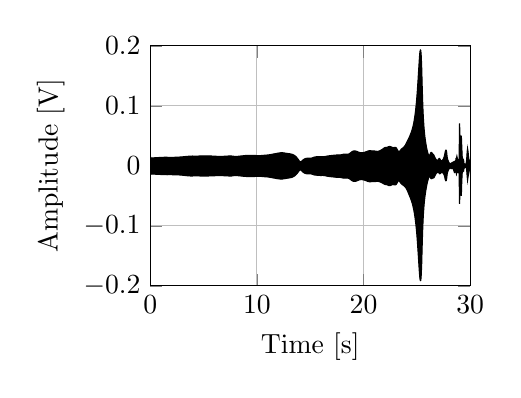
\begin{tikzpicture}

\begin{axis}[%
width=1.6in,
height=1.2in,
at={(0.758in,0.481in)},
scale only axis,
xmin=0,
xmax=30,
xmajorgrids,
ymin=-0.2,
ymax=0.2,
ymajorgrids,
xlabel={Time [s]},
ylabel={Amplitude [V]},
axis background/.style={fill=white}
]
\addplot[fill=black,draw=black,forget plot] plot table[row sep=crcr]{%
2.08333333333333e-05	0.0174441337585449\\
0.0417454218822439	0.0131838321685791\\
0.0834700104311544	0.0131036043167114\\
0.125194598980065	0.0131006240844727\\
0.166919187528975	0.0131523609161377\\
0.208643776077886	0.0131937265396118\\
0.250368364626797	0.013242244720459\\
0.292092953175707	0.0132843255996704\\
0.333817541724618	0.0133000612258911\\
0.375542130273528	0.0133227109909058\\
0.417266718822439	0.0133814811706543\\
0.458991307371349	0.0134208202362061\\
0.50071589592026	0.0134570598602295\\
0.54244048446917	0.0134916305541992\\
0.584165073018081	0.0135313272476196\\
0.625889661566991	0.0135787725448608\\
0.667614250115902	0.0136535167694092\\
0.709338838664812	0.0136919021606445\\
0.751063427213723	0.0137407779693604\\
0.792788015762633	0.01378333568573\\
0.834512604311544	0.0138405561447144\\
0.876237192860454	0.0138554573059082\\
0.917961781409365	0.0138992071151733\\
0.959686369958275	0.0139317512512207\\
1.00141095850719	0.0139665603637695\\
1.0431355470561	0.0140010118484497\\
1.08486013560501	0.0140565633773804\\
1.12658472415392	0.0140770673751831\\
1.16830931270283	0.0141662359237671\\
1.21003390125174	0.0141417980194092\\
1.25175848980065	0.014143705368042\\
1.29348307834956	0.0142022371292114\\
1.33520766689847	0.014235258102417\\
1.37693225544738	0.0142310857772827\\
1.41865684399629	0.0142514705657959\\
1.4603814325452	0.0142501592636108\\
1.50210602109411	0.0142426490783691\\
1.54383060964302	0.0142196416854858\\
1.58555519819193	0.0141897201538086\\
1.62727978674084	0.0141717195510864\\
1.66900437528975	0.0141562223434448\\
1.71072896383866	0.0141338109970093\\
1.75245355238758	0.0141158103942871\\
1.79417814093649	0.0141069889068604\\
1.8359027294854	0.014079213142395\\
1.87762731803431	0.0140920877456665\\
1.91935190658322	0.0140824317932129\\
1.96107649513213	0.014080286026001\\
2.00280108368104	0.0140819549560547\\
2.04452567222995	0.0140804052352905\\
2.08625026077886	0.0140907764434814\\
2.12797484932777	0.0141453742980957\\
2.16969943787668	0.0141212940216064\\
2.21142402642559	0.014117956161499\\
2.2531486149745	0.0141592025756836\\
2.29487320352341	0.0141942501068115\\
2.33659779207232	0.0142147541046143\\
2.37832238062123	0.014255166053772\\
2.42004696917014	0.0142718553543091\\
2.46177155771905	0.0143097639083862\\
2.50349614626796	0.0143415927886963\\
2.54522073481687	0.0143803358078003\\
2.58694532336579	0.0144282579421997\\
2.6286699119147	0.014466404914856\\
2.67039450046361	0.0145164728164673\\
2.71211908901252	0.0145268440246582\\
2.75384367756143	0.0145998001098633\\
2.79556826611034	0.014657735824585\\
2.83729285465925	0.0147078037261963\\
2.87901744320816	0.014757513999939\\
2.92074203175707	0.0148080587387085\\
2.96246662030598	0.0148706436157227\\
3.00419120885489	0.0149272680282593\\
3.0459157974038	0.0149846076965332\\
3.08764038595271	0.0150657892227173\\
3.12936497450162	0.0151398181915283\\
3.17108956305053	0.0152368545532227\\
3.21281415159944	0.0153077840805054\\
3.25453874014835	0.0153566598892212\\
3.29626332869726	0.0154335498809814\\
3.33798791724618	0.0155411958694458\\
3.37971250579509	0.0155764818191528\\
3.421437094344	0.0156253576278687\\
3.46316168289291	0.0156955718994141\\
3.50488627144182	0.015771746635437\\
3.54661085999073	0.0158456563949585\\
3.58833544853964	0.0159142017364502\\
3.63006003708855	0.0159842967987061\\
3.67178462563746	0.0160502195358276\\
3.71350921418637	0.0160926580429077\\
3.75523380273528	0.0161477327346802\\
3.79695839128419	0.01618492603302\\
3.8386829798331	0.0162196159362793\\
3.88040756838201	0.0162382125854492\\
3.92213215693092	0.0162550210952759\\
3.96385674547983	0.0162825584411621\\
4.00558133402874	0.0162662267684937\\
4.04730592257765	0.0162646770477295\\
4.08903051112656	0.0162562131881714\\
4.13075509967547	0.0162286758422852\\
4.17247968822439	0.0162371397018433\\
4.2142042767733	0.0162320137023926\\
4.25592886532221	0.0162011384963989\\
4.29765345387112	0.0161941051483154\\
4.33937804242003	0.0161887407302856\\
4.38110263096894	0.0161789655685425\\
4.42282721951785	0.0162254571914673\\
4.46455180806676	0.0162070989608765\\
4.50627639661567	0.0162445306777954\\
4.54800098516458	0.0162758827209473\\
4.58972557371349	0.0163146257400513\\
4.6314501622624	0.0163501501083374\\
4.67317475081131	0.0163940191268921\\
4.71489933936022	0.0164343118667603\\
4.75662392790913	0.0164703130722046\\
4.79834851645804	0.0165045261383057\\
4.84007310500695	0.0165075063705444\\
4.88179769355586	0.0165128707885742\\
4.92352228210478	0.0165145397186279\\
4.96524687065368	0.0165392160415649\\
5.0069714592026	0.0165344476699829\\
5.04869604775151	0.0165383815765381\\
5.09042063630042	0.0165327787399292\\
5.13214522484933	0.0165436267852783\\
5.17386981339824	0.0165482759475708\\
5.21559440194715	0.0165524482727051\\
5.25731899049606	0.0165770053863525\\
5.29904357904497	0.0165486335754395\\
5.34076816759388	0.016539454460144\\
5.38249275614279	0.0165292024612427\\
5.4242173446917	0.0165091753005981\\
5.46594193324061	0.01650071144104\\
5.50766652178952	0.0164941549301147\\
5.54939111033843	0.0164557695388794\\
5.59111569888734	0.0164422988891602\\
5.63284028743625	0.0164107084274292\\
5.67456487598516	0.0163847208023071\\
5.71628946453407	0.0163488388061523\\
5.75801405308299	0.0162984132766724\\
5.7997386416319	0.016254186630249\\
5.84146323018081	0.0161999464035034\\
5.88318781872972	0.0161627531051636\\
5.92491240727863	0.016115665435791\\
5.96663699582754	0.0160861015319824\\
6.00836158437645	0.0160255432128906\\
6.05008617292536	0.0159963369369507\\
6.09181076147427	0.0159608125686646\\
6.13353535002318	0.015892505645752\\
6.17525993857209	0.0158644914627075\\
6.216984527121	0.0158439874649048\\
6.25870911566991	0.0158376693725586\\
6.30043370421882	0.015795111656189\\
6.34215829276773	0.0157642364501953\\
6.38388288131664	0.0157539844512939\\
6.42560746986555	0.0157680511474609\\
6.46733205841446	0.0157626867294312\\
6.50905664696338	0.0157822370529175\\
6.55078123551229	0.0157889127731323\\
6.5925058240612	0.01578688621521\\
6.63423041261011	0.015788197517395\\
6.67595500115902	0.0158027410507202\\
6.71767958970793	0.0158090591430664\\
6.75940417825684	0.0158181190490723\\
6.80112876680575	0.0158118009567261\\
6.84285335535466	0.0158218145370483\\
6.88457794390357	0.0158369541168213\\
6.92630253245248	0.0158761739730835\\
6.96802712100139	0.0158882141113281\\
7.0097517095503	0.0159152746200562\\
7.05147629809921	0.015964150428772\\
7.09320088664812	0.0159767866134644\\
7.13492547519703	0.0160250663757324\\
7.17665006374594	0.0161073207855225\\
7.21837465229485	0.0161528587341309\\
7.26009924084376	0.0162261724472046\\
7.30182382939268	0.0163071155548096\\
7.34354841794159	0.0163383483886719\\
7.3852730064905	0.016379714012146\\
7.42699759503941	0.0164109468460083\\
7.46872218358832	0.0164202451705933\\
7.51044677213723	0.01641845703125\\
7.55217136068614	0.0163893699645996\\
7.59389594923505	0.0163551568984985\\
7.63562053778396	0.016291618347168\\
7.67734512633287	0.0162198543548584\\
7.71906971488178	0.0161285400390625\\
7.76079430343069	0.016048789024353\\
7.8025188919796	0.0159471035003662\\
7.84424348052851	0.0158181190490723\\
7.88596806907742	0.0157514810562134\\
7.92769265762633	0.0156846046447754\\
7.96941724617524	0.0156430006027222\\
8.01114183472416	0.0156441926956177\\
8.05286642327307	0.015630841255188\\
8.09459101182198	0.0156680345535278\\
8.13631560037089	0.015711784362793\\
8.1780401889198	0.0157798528671265\\
8.21976477746871	0.0158299207687378\\
8.26148936601762	0.0159074068069458\\
8.30321395456653	0.0159891843795776\\
8.34493854311544	0.01605224609375\\
8.38666313166435	0.0161564350128174\\
8.42838772021326	0.0162137746810913\\
8.47011230876217	0.0163058042526245\\
8.51183689731108	0.0163658857345581\\
8.55356148585999	0.0164523124694824\\
8.5952860744089	0.0164806842803955\\
8.63701066295781	0.0166155099868774\\
8.67873525150672	0.0166575908660889\\
8.72045984005563	0.0167548656463623\\
8.76218442860454	0.016825795173645\\
8.80390901715345	0.0169020891189575\\
8.84563360570237	0.0169821977615356\\
8.88735819425128	0.0170701742172241\\
8.92908278280018	0.0171375274658203\\
8.9708073713491	0.0171587467193604\\
9.01253195989801	0.017237663269043\\
9.05425654844692	0.0172935724258423\\
9.09598113699583	0.0173218250274658\\
9.13770572554474	0.0173497200012207\\
9.17943031409365	0.0173822641372681\\
9.22115490264256	0.0174020528793335\\
9.26287949119147	0.0174028873443604\\
9.30460407974038	0.0174020528793335\\
9.34632866828929	0.017397403717041\\
9.3880532568382	0.017382025718689\\
9.42977784538711	0.0173323154449463\\
9.47150243393602	0.0173298120498657\\
9.51322702248493	0.0173071622848511\\
9.55495161103384	0.0172981023788452\\
9.59667619958275	0.0172533988952637\\
9.63840078813166	0.0172268152236938\\
9.68012537668058	0.0172126293182373\\
9.72184996522949	0.0172011852264404\\
9.7635745537784	0.0171804428100586\\
9.80529914232731	0.0171520709991455\\
9.84702373087622	0.0171386003494263\\
9.88874831942513	0.0171166658401489\\
9.93047290797404	0.0170993804931641\\
9.97219749652295	0.0170501470565796\\
10.0139220850719	0.0170356035232544\\
10.0556466736208	0.0170102119445801\\
10.0973712621697	0.0169705152511597\\
10.1390958507186	0.0169491767883301\\
10.1808204392675	0.0169264078140259\\
10.2225450278164	0.0169349908828735\\
10.2642696163653	0.016948938369751\\
10.3059942049142	0.0169826745986938\\
10.3477187934631	0.0170327425003052\\
10.3894433820121	0.0170915126800537\\
10.431167970561	0.0171574354171753\\
10.4728925591099	0.0172317028045654\\
10.5146171476588	0.0172722339630127\\
10.5563417362077	0.0173627138137817\\
10.5980663247566	0.0174278020858765\\
10.6397909133055	0.0175130367279053\\
10.6815155018544	0.0175483226776123\\
10.7232400904033	0.0176342725753784\\
10.7649646789523	0.0176903009414673\\
10.8066892675012	0.0177403688430786\\
10.8484138560501	0.0177834033966064\\
10.890138444599	0.0178585052490234\\
10.9318630331479	0.0179126262664795\\
10.9735876216968	0.0179930925369263\\
11.0153122102457	0.0180377960205078\\
11.0570367987946	0.0181233882904053\\
11.0987613873435	0.0181983709335327\\
11.1404859758924	0.0183128118515015\\
11.1822105644414	0.0184154510498047\\
11.2239351529903	0.0185511112213135\\
11.2656597415392	0.0186648368835449\\
11.3073843300881	0.0188018083572388\\
11.349108918637	0.0189625024795532\\
11.3908335071859	0.0190943479537964\\
11.4325580957348	0.0192328691482544\\
11.4742826842837	0.0194246768951416\\
11.5160072728326	0.0195508003234863\\
11.5577318613816	0.019692063331604\\
11.5994564499305	0.0198198556900024\\
11.6411810384794	0.0199755430221558\\
11.6829056270283	0.0201060771942139\\
11.7246302155772	0.0202442407608032\\
11.7663548041261	0.0203926563262939\\
11.808079392675	0.0205307006835938\\
11.8498039812239	0.0206559896469116\\
11.8915285697728	0.0208258628845215\\
11.9332531583217	0.0209463834762573\\
11.9749777468707	0.0210902690887451\\
12.0167023354196	0.0212063789367676\\
12.0584269239685	0.0213172435760498\\
12.1001515125174	0.0214052200317383\\
12.1418761010663	0.0215300321578979\\
12.1836006896152	0.0216346979141235\\
12.2253252781641	0.0217214822769165\\
12.267049866713	0.0217512845993042\\
12.3087744552619	0.0217386484146118\\
12.3504990438108	0.0217629671096802\\
12.3922236323598	0.0217190980911255\\
12.4339482209087	0.0217164754867554\\
12.4756728094576	0.0216211080551147\\
12.5173973980065	0.0215216875076294\\
12.5591219865554	0.0214111804962158\\
12.6008465751043	0.0212830305099487\\
12.6425711636532	0.0211762189865112\\
12.6842957522021	0.0210355520248413\\
12.726020340751	0.0209170579910278\\
12.7677449293	0.0208185911178589\\
12.8094695178489	0.0207177400588989\\
12.8511941063978	0.0206308364868164\\
12.8929186949467	0.0205261707305908\\
12.9346432834956	0.0204188823699951\\
12.9763678720445	0.0203160047531128\\
13.0180924605934	0.0202019214630127\\
13.0598170491423	0.020089864730835\\
13.1015416376912	0.0199722051620483\\
13.1432662262401	0.0198445320129395\\
13.1849908147891	0.0197038650512695\\
13.226715403338	0.0195189714431763\\
13.2684399918869	0.0193073749542236\\
13.3101645804358	0.0190596580505371\\
13.3518891689847	0.0188181400299072\\
13.3936137575336	0.0185122489929199\\
13.4353383460825	0.0181918144226074\\
13.4770629346314	0.0177853107452393\\
13.5187875231803	0.0173110961914063\\
13.5605121117293	0.0167787075042725\\
13.6022367002782	0.0161740779876709\\
13.6439612888271	0.0155293941497803\\
13.685685877376	0.0147796869277954\\
13.7274104659249	0.0139639377593994\\
13.7691350544738	0.0130655765533447\\
13.8108596430227	0.0121190547943115\\
13.8525842315716	0.011111855506897\\
13.8943088201205	0.0100915431976318\\
13.9360334086694	0.00906765460968018\\
13.9777579972184	0.0081101655960083\\
14.0194825857673	0.00735759735107422\\
14.0612071743162	0.00674760341644287\\
14.1029317628651	0.00652647018432617\\
14.144656351414	0.00688815116882324\\
14.1863809399629	0.00745463371276855\\
14.2281055285118	0.00815272331237793\\
14.2698301170607	0.00885546207427979\\
14.3115547056096	0.00954830646514893\\
14.3532792941586	0.0101321935653687\\
14.3950038827075	0.0106920003890991\\
14.4367284712564	0.0111517906188965\\
14.4784530598053	0.0115351676940918\\
14.5201776483542	0.0118722915649414\\
14.5619022369031	0.0121043920516968\\
14.603626825452	0.0123043060302734\\
14.6453514140009	0.0124328136444092\\
14.6870760025498	0.0125536918640137\\
14.7288005910988	0.0126279592514038\\
14.7705251796477	0.0126522779464722\\
14.8122497681966	0.0126771926879883\\
14.8539743567455	0.0126643180847168\\
14.8956989452944	0.0126442909240723\\
14.9374235338433	0.0126314163208008\\
14.9791481223922	0.0126005411148071\\
15.0208727109411	0.0125870704650879\\
15.06259729949	0.0126197338104248\\
15.1043218880389	0.0127360820770264\\
15.1460464765879	0.0129470825195313\\
15.1877710651368	0.0131411552429199\\
15.2294956536857	0.0134528875350952\\
15.2712202422346	0.0137631893157959\\
15.3129448307835	0.014081597328186\\
15.3546694193324	0.0143324136734009\\
15.3963940078813	0.0145440101623535\\
15.4381185964302	0.0147069692611694\\
15.4798431849791	0.014826774597168\\
15.521567773528	0.0149147510528564\\
15.563292362077	0.0150187015533447\\
15.6050169506259	0.0150867700576782\\
15.6467415391748	0.0151418447494507\\
15.6884661277237	0.0152006149291992\\
15.7301907162726	0.0152875185012817\\
15.7719153048215	0.015317440032959\\
15.8136398933704	0.0153570175170898\\
15.8553644819193	0.0153845548629761\\
15.8970890704682	0.0154201984405518\\
15.9388136590172	0.0154287815093994\\
15.9805382475661	0.0154200792312622\\
16.022262836115	0.0154227018356323\\
16.0639874246639	0.0153900384902954\\
16.1057120132128	0.0153504610061646\\
16.1474366017617	0.0152820348739624\\
16.1891611903106	0.0152740478515625\\
16.2308857788595	0.0152736902236938\\
16.2726103674084	0.0152853727340698\\
16.3143349559573	0.0153579711914063\\
16.3560595445063	0.0154263973236084\\
16.3977841330552	0.0155422687530518\\
16.4395087216041	0.0156645774841309\\
16.481233310153	0.015790581703186\\
16.5229578987019	0.0159449577331543\\
16.5646824872508	0.0161056518554688\\
16.6064070757997	0.0162507295608521\\
16.6481316643486	0.0163685083389282\\
16.6898562528975	0.0164653062820435\\
16.7315808414465	0.0165603160858154\\
16.7733054299954	0.0167076587677002\\
16.8150300185443	0.0167895555496216\\
16.8567546070932	0.0168788433074951\\
16.8984791956421	0.0169848203659058\\
16.940203784191	0.017051100730896\\
16.9819283727399	0.017139196395874\\
17.0236529612888	0.0172312259674072\\
17.0653775498377	0.0173563957214355\\
17.1071021383867	0.0174448490142822\\
17.1488267269356	0.0174803733825684\\
17.1905513154845	0.0175639390945435\\
17.2322759040334	0.0176322460174561\\
17.2740004925823	0.0177028179168701\\
17.3157250811312	0.017791748046875\\
17.3574496696801	0.0178496837615967\\
17.399174258229	0.0178979635238647\\
17.4408988467779	0.017961859703064\\
17.4826234353268	0.018022894859314\\
17.5243480238758	0.018062949180603\\
17.5660726124247	0.01810622215271\\
17.6077972009736	0.0180763006210327\\
17.6495217895225	0.0180815458297729\\
17.6912463780714	0.0180732011795044\\
17.7329709666203	0.0180991888046265\\
17.7746955551692	0.0181357860565186\\
17.8164201437181	0.018202543258667\\
17.858144732267	0.0183231830596924\\
17.8998693208159	0.0184512138366699\\
17.9415939093649	0.0185703039169312\\
17.9833184979138	0.0187492370605469\\
18.0250430864627	0.0189353227615356\\
18.0667676750116	0.0190675258636475\\
18.1084922635605	0.0192264318466187\\
18.1502168521094	0.0192973613739014\\
18.1919414406583	0.0193362236022949\\
18.2336660292072	0.0193533897399902\\
18.2753906177561	0.0193248987197876\\
18.3171152063051	0.0193346738815308\\
18.358839794854	0.0192720890045166\\
18.4005643834029	0.0192611217498779\\
18.4422889719518	0.0192636251449585\\
18.4840135605007	0.0192739963531494\\
18.5257381490496	0.0192903280258179\\
18.5674627375985	0.0194275379180908\\
18.6091873261474	0.0196996927261353\\
18.6509119146963	0.0200306177139282\\
18.6926365032453	0.0204979181289673\\
18.7343610917942	0.02104651927948\\
18.7760856803431	0.0216186046600342\\
18.817810268892	0.0222443342208862\\
18.8595348574409	0.0227910280227661\\
18.9012594459898	0.0233092308044434\\
18.9429840345387	0.023730993270874\\
18.9847086230876	0.0240856409072876\\
19.0264332116365	0.0244448184967041\\
19.0681578001854	0.0246785879135132\\
19.1098823887344	0.0248157978057861\\
19.1516069772833	0.0248291492462158\\
19.1933315658322	0.0247887372970581\\
19.2350561543811	0.0246955156326294\\
19.27678074293	0.0245308876037598\\
19.3185053314789	0.0243546962738037\\
19.3602299200278	0.0240871906280518\\
19.4019545085767	0.0237839221954346\\
19.4436790971256	0.0234526395797729\\
19.4854036856745	0.0231184959411621\\
19.5271282742235	0.022815465927124\\
19.5688528627724	0.0225284099578857\\
19.6105774513213	0.0223060846328735\\
19.6523020398702	0.0221070051193237\\
19.6940266284191	0.0219635963439941\\
19.735751216968	0.0218530893325806\\
19.7774758055169	0.0217581987380981\\
19.8192003940658	0.0217596292495728\\
19.8609249826147	0.0217828750610352\\
19.9026495711637	0.0218667984008789\\
19.9443741597126	0.0219509601593018\\
19.9860987482615	0.0220874547958374\\
20.0278233368104	0.0222543478012085\\
20.0695479253593	0.0224721431732178\\
20.1112725139082	0.0226690769195557\\
20.1529971024571	0.0229157209396362\\
20.194721691006	0.0231697559356689\\
20.2364462795549	0.0234352350234985\\
20.2781708681038	0.0237188339233398\\
20.3198954566528	0.0240160226821899\\
20.3616200452017	0.0242964029312134\\
20.4033446337506	0.024566650390625\\
20.4450692222995	0.0247782468795776\\
20.4867938108484	0.0249801874160767\\
20.5285183993973	0.025060772895813\\
20.5702429879462	0.0250948667526245\\
20.6119675764951	0.0251015424728394\\
20.653692165044	0.025084376335144\\
20.695416753593	0.0250260829925537\\
20.7371413421419	0.0249568223953247\\
20.7788659306908	0.0249083042144775\\
20.8205905192397	0.0248545408248901\\
20.8623151077886	0.0248538255691528\\
20.9040396963375	0.0248321294784546\\
20.9457642848864	0.0248123407363892\\
20.9874888734353	0.0247715711593628\\
21.0292134619842	0.0246872901916504\\
21.0709380505331	0.0245916843414307\\
21.1126626390821	0.0244895219802856\\
21.154387227631	0.0243560075759888\\
21.1961118161799	0.0242257118225098\\
21.2378364047288	0.0241231918334961\\
21.2795609932777	0.0240743160247803\\
21.3212855818266	0.0240955352783203\\
21.3630101703755	0.0242211818695068\\
21.4047347589244	0.0243576765060425\\
21.4464593474733	0.0245411396026611\\
21.4881839360223	0.0248323678970337\\
21.5299085245712	0.0251299142837524\\
21.5716331131201	0.0254895687103271\\
21.613357701669	0.0259164571762085\\
21.6550822902179	0.0263410806655884\\
21.6968068787668	0.0268235206604004\\
21.7385314673157	0.0273033380508423\\
21.7802560558646	0.0278036594390869\\
21.8219806444135	0.0282833576202393\\
21.8637052329624	0.0288461446762085\\
21.9054298215114	0.0293409824371338\\
21.9471544100603	0.0298067331314087\\
21.9888789986092	0.0302213430404663\\
22.0306035871581	0.0305540561676025\\
22.072328175707	0.0307530164718628\\
22.1140527642559	0.0307987928390503\\
22.1557773528048	0.030825138092041\\
22.1975019413537	0.0308418273925781\\
22.2392265299026	0.0311071872711182\\
22.2809511184516	0.0313805341720581\\
22.3226757070005	0.0317173004150391\\
22.3644002955494	0.0320000648498535\\
22.4061248840983	0.0321570634841919\\
22.4478494726472	0.0321915149688721\\
22.4895740611961	0.0321606397628784\\
22.531298649745	0.031922459602356\\
22.5730232382939	0.0316141843795776\\
22.6147478268428	0.0312548875808716\\
22.6564724153917	0.0308171510696411\\
22.6981970039407	0.0305826663970947\\
22.7399215924896	0.0304679870605469\\
22.7816461810385	0.0303603410720825\\
22.8233707695874	0.0304563045501709\\
22.8650953581363	0.0305367708206177\\
22.9068199466852	0.0306057929992676\\
22.9485445352341	0.0306912660598755\\
22.990269123783	0.0306066274642944\\
23.0319937123319	0.0304591655731201\\
23.0737183008809	0.0297863483428955\\
23.1154428894298	0.0285071134567261\\
23.1571674779787	0.027154803276062\\
23.1988920665276	0.0259910821914673\\
23.2406166550765	0.0244603157043457\\
23.2823412436254	0.0236220359802246\\
23.3240658321743	0.0235285758972168\\
23.3657904207232	0.0241098403930664\\
23.4075150092721	0.0248513221740723\\
23.449239597821	0.0258579254150391\\
23.49096418637	0.0267441272735596\\
23.5326887749189	0.0276174545288086\\
23.5744133634678	0.0282967090606689\\
23.6161379520167	0.0288980007171631\\
23.6578625405656	0.0294115543365479\\
23.6995871291145	0.0299835205078125\\
23.7413117176634	0.0305644273757935\\
23.7830363062123	0.0313618183135986\\
23.8247608947612	0.0322580337524414\\
23.8664854833102	0.0332018136978149\\
23.9082100718591	0.0342499017715454\\
23.949934660408	0.035599946975708\\
23.9916592489569	0.0370364189147949\\
24.0333838375058	0.0383732318878174\\
24.0751084260547	0.0398944616317749\\
24.1168330146036	0.041479229927063\\
24.1585576031525	0.0429228544235229\\
24.2002821917014	0.0444319248199463\\
24.2420067802503	0.0459293127059937\\
24.2837313687993	0.047610878944397\\
24.3254559573482	0.0492688417434692\\
24.3671805458971	0.0510417222976685\\
24.408905134446	0.0529109239578247\\
24.4506297229949	0.0548422336578369\\
24.4923543115438	0.056898832321167\\
24.5340789000927	0.0591094493865967\\
24.5758034886416	0.0617804527282715\\
24.6175280771905	0.0645843744277954\\
24.6592526657395	0.0677156448364258\\
24.7009772542884	0.0712670087814331\\
24.7427018428373	0.0752949714660645\\
24.7844264313862	0.0799596309661865\\
24.8261510199351	0.0852384567260742\\
24.867875608484	0.0909876823425293\\
24.9096001970329	0.0979855060577393\\
24.9513247855818	0.105462312698364\\
24.9930493741307	0.114107251167297\\
25.0347739626796	0.123892664909363\\
25.0764985512286	0.1347895860672\\
25.1182231397775	0.146229147911072\\
25.1599477283264	0.158706545829773\\
25.2016723168753	0.170397281646729\\
25.2433969054242	0.181927919387817\\
25.2851214939731	0.190452098846436\\
25.326846082522	0.192880272865295\\
25.3685706710709	0.192157387733459\\
25.4102952596198	0.181955933570862\\
25.4520198481687	0.162297606468201\\
25.4937444367177	0.13434636592865\\
25.5354690252666	0.109553933143616\\
25.5771936138155	0.0896941423416138\\
25.6189182023644	0.0760148763656616\\
25.6606427909133	0.0651895999908447\\
25.7023673794622	0.0563890933990479\\
25.7440919680111	0.0492444038391113\\
25.78581655656	0.043710470199585\\
25.8275411451089	0.0384472608566284\\
25.8692657336579	0.0339940786361694\\
25.9109903222068	0.0300600528717041\\
25.9527149107557	0.0264880657196045\\
25.9944394993046	0.0233311653137207\\
26.0361640878535	0.0206685066223145\\
26.0778886764024	0.0186737775802612\\
26.1196132649513	0.0171686410903931\\
26.1613378535002	0.0166844129562378\\
26.2030624420491	0.017844557762146\\
26.2447870305981	0.0197421312332153\\
26.286511619147	0.0215028524398804\\
26.3282362076959	0.0223579406738281\\
26.3699607962448	0.0223031044006348\\
26.4116853847937	0.0217078924179077\\
26.4534099733426	0.0204193592071533\\
26.4951345618915	0.0195810794830322\\
26.5368591504404	0.0191034078598022\\
26.5785837389893	0.0182909965515137\\
26.6203083275383	0.01659095287323\\
26.6620329160872	0.0147438049316406\\
26.7037575046361	0.0134490728378296\\
26.745482093185	0.012037992477417\\
26.7872066817339	0.0107738971710205\\
26.8289312702828	0.00990462303161621\\
26.8706558588317	0.00957143306732178\\
26.9123804473806	0.00931215286254883\\
26.9541050359295	0.0092695951461792\\
26.9958296244784	0.0102084875106812\\
27.0375542130274	0.0113158226013184\\
27.0792788015763	0.0121122598648071\\
27.1210033901252	0.0121549367904663\\
27.1627279786741	0.0111083984375\\
27.204452567223	0.00957083702087402\\
27.2461771557719	0.00859379768371582\\
27.2879017443208	0.00834882259368896\\
27.3296263328697	0.00859546661376953\\
27.3713509214186	0.0090184211730957\\
27.4130755099675	0.00977170467376709\\
27.4548000985165	0.0107346773147583\\
27.4965246870654	0.012182354927063\\
27.5382492756143	0.0141066312789917\\
27.5799738641632	0.0166143178939819\\
27.6216984527121	0.0203871726989746\\
27.663423041261	0.0240563154220581\\
27.7051476298099	0.0260938405990601\\
27.7468722183588	0.0261249542236328\\
27.7885968069077	0.0226942300796509\\
27.8303213954567	0.0153995752334595\\
27.8720459840056	0.0115272998809814\\
27.9137705725545	0.00934135913848877\\
27.9554951611034	0.00725364685058594\\
27.9972197496523	0.00573289394378662\\
28.0389443382012	0.00476109981536865\\
28.0806689267501	0.00405430793762207\\
28.122393515299	0.00347089767456055\\
28.1641181038479	0.00348937511444092\\
28.2058426923968	0.0043492317199707\\
28.2475672809458	0.00484251976013184\\
28.2892918694947	0.00487172603607178\\
28.3310164580436	0.00547254085540771\\
28.3727410465925	0.00589895248413086\\
28.4144656351414	0.00629270076751709\\
28.4561902236903	0.00670242309570313\\
28.4979148122392	0.00694727897644043\\
28.5396394007881	0.00746893882751465\\
28.581363989337	0.00698328018188477\\
28.623088577886	0.00598013401031494\\
28.6648131664349	0.0123151540756226\\
28.7065377549838	0.0124528408050537\\
28.7482623435327	0.0158895254135132\\
28.7899869320816	0.0123809576034546\\
28.8317115206305	0.00990724563598633\\
28.8734361091794	0.0101600885391235\\
28.9151606977283	0.00902903079986572\\
28.9568852862772	0.00959169864654541\\
28.9986098748261	0.0708549022674561\\
29.0403344633751	0.0490773916244507\\
29.082059051924	0.0367391109466553\\
29.1237836404729	0.0392665863037109\\
29.1655082290218	0.0501984357833862\\
29.2072328175707	0.0316517353057861\\
29.2489574061196	0.0146907567977905\\
29.2906819946685	0.0124069452285767\\
29.3324065832174	0.0109615325927734\\
29.3741311717663	0.00983536243438721\\
29.4158557603153	0.00371837615966797\\
29.4575803488642	0.00346684455871582\\
29.4993049374131	0.0025477409362793\\
29.541029525962	0.0020139217376709\\
29.5827541145109	0.00222396850585938\\
29.6244787030598	0.0047835111618042\\
29.6662032916087	0.0106549263000488\\
29.7079278801576	0.0227276086807251\\
29.7496524687065	0.0288950204849243\\
29.7913770572554	0.0240693092346191\\
29.8331016458044	0.0165066719055176\\
29.8748262343533	0.0114091634750366\\
29.9165508229022	0.00875699520111084\\
29.9582754114511	0.00749635696411133\\
30	0.00196146965026855\\
}
\closedcycle;
\addplot[fill=black,draw=black,forget plot] plot table[row sep=crcr]{%
2.08333333333333e-05	-0.0159932374954224\\
0.0417454218822439	-0.0136831998825073\\
0.0834700104311544	-0.0136864185333252\\
0.125194598980065	-0.0137081146240234\\
0.166919187528975	-0.0137027502059937\\
0.208643776077886	-0.0137177705764771\\
0.250368364626797	-0.0137653350830078\\
0.292092953175707	-0.0137816667556763\\
0.333817541724618	-0.0138300657272339\\
0.375542130273528	-0.0138695240020752\\
0.417266718822439	-0.0139075517654419\\
0.458991307371349	-0.0139497518539429\\
0.50071589592026	-0.0140053033828735\\
0.54244048446917	-0.0140515565872192\\
0.584165073018081	-0.0140962600708008\\
0.625889661566991	-0.0141353607177734\\
0.667614250115902	-0.0141550302505493\\
0.709338838664812	-0.0141642093658447\\
0.751063427213723	-0.0142364501953125\\
0.792788015762633	-0.0142496824264526\\
0.834512604311544	-0.0143007040023804\\
0.876237192860454	-0.0143524408340454\\
0.917961781409365	-0.0143682956695557\\
0.959686369958275	-0.0144027471542358\\
1.00141095850719	-0.0144290924072266\\
1.0431355470561	-0.0144684314727783\\
1.08486013560501	-0.0145009756088257\\
1.12658472415392	-0.0145292282104492\\
1.16830931270283	-0.0145310163497925\\
1.21003390125174	-0.0145913362503052\\
1.25175848980065	-0.0146056413650513\\
1.29348307834956	-0.014609694480896\\
1.33520766689847	-0.014613151550293\\
1.37693225544738	-0.0146564245223999\\
1.41865684399629	-0.0147069692611694\\
1.4603814325452	-0.0147548913955688\\
1.50210602109411	-0.0147720575332642\\
1.54383060964302	-0.0147882699966431\\
1.58555519819193	-0.0148137807846069\\
1.62727978674084	-0.0147954225540161\\
1.66900437528975	-0.0147997140884399\\
1.71072896383866	-0.014802098274231\\
1.75245355238758	-0.0147850513458252\\
1.79417814093649	-0.0147900581359863\\
1.8359027294854	-0.0147967338562012\\
1.87762731803431	-0.0147658586502075\\
1.91935190658322	-0.0147805213928223\\
1.96107649513213	-0.0147795677185059\\
2.00280108368104	-0.0147765874862671\\
2.04452567222995	-0.0148054361343384\\
2.08625026077886	-0.0148167610168457\\
2.12797484932777	-0.0148104429244995\\
2.16969943787668	-0.014845609664917\\
2.21142402642559	-0.0148526430130005\\
2.2531486149745	-0.0148493051528931\\
2.29487320352341	-0.0148800611495972\\
2.33659779207232	-0.0149073600769043\\
2.37832238062123	-0.0149215459823608\\
2.42004696917014	-0.0149686336517334\\
2.46177155771905	-0.0149891376495361\\
2.50349614626796	-0.0150300264358521\\
2.54522073481687	-0.015070915222168\\
2.58694532336579	-0.0150928497314453\\
2.6286699119147	-0.0151451826095581\\
2.67039450046361	-0.0151525735855103\\
2.71211908901252	-0.0152038335800171\\
2.75384367756143	-0.0152643918991089\\
2.79556826611034	-0.0153129100799561\\
2.83729285465925	-0.0153428316116333\\
2.87901744320816	-0.0154058933258057\\
2.92074203175707	-0.015446662902832\\
2.96246662030598	-0.0155152082443237\\
3.00419120885489	-0.0156008005142212\\
3.0459157974038	-0.015687108039856\\
3.08764038595271	-0.015765905380249\\
3.12936497450162	-0.0158531665802002\\
3.17108956305053	-0.0159111022949219\\
3.21281415159944	-0.0159949064254761\\
3.25453874014835	-0.0161058902740479\\
3.29626332869726	-0.0161623954772949\\
3.33798791724618	-0.0162557363510132\\
3.37971250579509	-0.0163384675979614\\
3.421437094344	-0.0164409875869751\\
3.46316168289291	-0.0165195465087891\\
3.50488627144182	-0.0165740251541138\\
3.54661085999073	-0.0166549682617188\\
3.58833544853964	-0.0167381763458252\\
3.63006003708855	-0.0167884826660156\\
3.67178462563746	-0.0168477296829224\\
3.71350921418637	-0.016872763633728\\
3.75523380273528	-0.0168941020965576\\
3.79695839128419	-0.0169187784194946\\
3.8386829798331	-0.0169479846954346\\
3.88040756838201	-0.0169333219528198\\
3.92213215693092	-0.016893744468689\\
3.96385674547983	-0.0169346332550049\\
4.00558133402874	-0.0168807506561279\\
4.04730592257765	-0.0168675184249878\\
4.08903051112656	-0.0168465375900269\\
4.13075509967547	-0.0168452262878418\\
4.17247968822439	-0.0168131589889526\\
4.2142042767733	-0.0167852640151978\\
4.25592886532221	-0.0167598724365234\\
4.29765345387112	-0.0167505741119385\\
4.33937804242003	-0.016740083694458\\
4.38110263096894	-0.0167372226715088\\
4.42282721951785	-0.0167292356491089\\
4.46455180806676	-0.0167250633239746\\
4.50627639661567	-0.0167497396469116\\
4.54800098516458	-0.0167809724807739\\
4.58972557371349	-0.0168344974517822\\
4.6314501622624	-0.0168977975845337\\
4.67317475081131	-0.0169267654418945\\
4.71489933936022	-0.0169526338577271\\
4.75662392790913	-0.0169451236724854\\
4.79834851645804	-0.0169491767883301\\
4.84007310500695	-0.0169534683227539\\
4.88179769355586	-0.0169605016708374\\
4.92352228210478	-0.0169579982757568\\
4.96524687065368	-0.0169459581375122\\
5.0069714592026	-0.0169612169265747\\
5.04869604775151	-0.0169461965560913\\
5.09042063630042	-0.016968846321106\\
5.13214522484933	-0.0169471502304077\\
5.17386981339824	-0.0169591903686523\\
5.21559440194715	-0.016942024230957\\
5.25731899049606	-0.0169354677200317\\
5.29904357904497	-0.0169334411621094\\
5.34076816759388	-0.016936182975769\\
5.38249275614279	-0.0169117450714111\\
5.4242173446917	-0.0169116258621216\\
5.46594193324061	-0.0169053077697754\\
5.50766652178952	-0.01686692237854\\
5.54939111033843	-0.0168808698654175\\
5.59111569888734	-0.0168665647506714\\
5.63284028743625	-0.0168148279190063\\
5.67456487598516	-0.0167924165725708\\
5.71628946453407	-0.0167427062988281\\
5.75801405308299	-0.0167151689529419\\
5.7997386416319	-0.0166959762573242\\
5.84146323018081	-0.0166800022125244\\
5.88318781872972	-0.0166391134262085\\
5.92491240727863	-0.0166083574295044\\
5.96663699582754	-0.0165565013885498\\
6.00836158437645	-0.016548752784729\\
6.05008617292536	-0.0165069103240967\\
6.09181076147427	-0.0164694786071777\\
6.13353535002318	-0.016451358795166\\
6.17525993857209	-0.0164226293563843\\
6.216984527121	-0.0163737535476685\\
6.25870911566991	-0.0163513422012329\\
6.30043370421882	-0.0163525342941284\\
6.34215829276773	-0.0163525342941284\\
6.38388288131664	-0.0163518190383911\\
6.42560746986555	-0.0163501501083374\\
6.46733205841446	-0.0163429975509644\\
6.50905664696338	-0.0163670778274536\\
6.55078123551229	-0.0163668394088745\\
6.5925058240612	-0.0163979530334473\\
6.63423041261011	-0.0164004564285278\\
6.67595500115902	-0.0164167881011963\\
6.71767958970793	-0.01643967628479\\
6.75940417825684	-0.0164421796798706\\
6.80112876680575	-0.0164488554000854\\
6.84285335535466	-0.016448974609375\\
6.88457794390357	-0.016472339630127\\
6.92630253245248	-0.0165094137191772\\
6.96802712100139	-0.0165352821350098\\
7.0097517095503	-0.0165783166885376\\
7.05147629809921	-0.0166103839874268\\
7.09320088664812	-0.0166771411895752\\
7.13492547519703	-0.0167235136032104\\
7.17665006374594	-0.016762375831604\\
7.21837465229485	-0.0168224573135376\\
7.26009924084376	-0.0168670415878296\\
7.30182382939268	-0.0168749094009399\\
7.34354841794159	-0.0169117450714111\\
7.3852730064905	-0.0169516801834106\\
7.42699759503941	-0.0169820785522461\\
7.46872218358832	-0.0169767141342163\\
7.51044677213723	-0.0169795751571655\\
7.55217136068614	-0.0169461965560913\\
7.59389594923505	-0.0169112682342529\\
7.63562053778396	-0.016893744468689\\
7.67734512633287	-0.0167742967605591\\
7.71906971488178	-0.016714334487915\\
7.76079430343069	-0.0166012048721313\\
7.8025188919796	-0.0164294242858887\\
7.84424348052851	-0.0163884162902832\\
7.88596806907742	-0.0163111686706543\\
7.92769265762633	-0.0162628889083862\\
7.96941724617524	-0.0162183046340942\\
8.01114183472416	-0.0162019729614258\\
8.05286642327307	-0.0162206888198853\\
8.09459101182198	-0.0162594318389893\\
8.13631560037089	-0.0162904262542725\\
8.1780401889198	-0.0163576602935791\\
8.21976477746871	-0.0164244174957275\\
8.26148936601762	-0.0165115594863892\\
8.30321395456653	-0.0165975093841553\\
8.34493854311544	-0.0166696310043335\\
8.38666313166435	-0.0167193412780762\\
8.42838772021326	-0.0168086290359497\\
8.47011230876217	-0.0168790817260742\\
8.51183689731108	-0.0169645547866821\\
8.55356148585999	-0.0170485973358154\\
8.5952860744089	-0.017114520072937\\
8.63701066295781	-0.0171991586685181\\
8.67873525150672	-0.0172797441482544\\
8.72045984005563	-0.0173673629760742\\
8.76218442860454	-0.0174151659011841\\
8.80390901715345	-0.0174990892410278\\
8.84563360570237	-0.0175384283065796\\
8.88735819425128	-0.0175958871841431\\
8.92908278280018	-0.0176502466201782\\
8.9708073713491	-0.0177098512649536\\
9.01253195989801	-0.0177485942840576\\
9.05425654844692	-0.0177981853485107\\
9.09598113699583	-0.017824649810791\\
9.13770572554474	-0.0178617238998413\\
9.17943031409365	-0.017900824546814\\
9.22115490264256	-0.017920970916748\\
9.26287949119147	-0.017920970916748\\
9.30460407974038	-0.0179229974746704\\
9.34632866828929	-0.0179156064987183\\
9.3880532568382	-0.0178991556167603\\
9.42977784538711	-0.0179009437561035\\
9.47150243393602	-0.0178804397583008\\
9.51322702248493	-0.0178624391555786\\
9.55495161103384	-0.017827033996582\\
9.59667619958275	-0.0178166627883911\\
9.63840078813166	-0.0177962779998779\\
9.68012537668058	-0.0177731513977051\\
9.72184996522949	-0.0177674293518066\\
9.7635745537784	-0.0177444219589233\\
9.80529914232731	-0.0177211761474609\\
9.84702373087622	-0.0176931619644165\\
9.88874831942513	-0.0176559686660767\\
9.93047290797404	-0.0176379680633545\\
9.97219749652295	-0.017622709274292\\
10.0139220850719	-0.0175876617431641\\
10.0556466736208	-0.0175426006317139\\
10.0973712621697	-0.0175328254699707\\
10.1390958507186	-0.017499566078186\\
10.1808204392675	-0.0175129175186157\\
10.2225450278164	-0.0174999237060547\\
10.2642696163653	-0.0175207853317261\\
10.3059942049142	-0.0175470113754272\\
10.3477187934631	-0.0176101922988892\\
10.3894433820121	-0.0176711082458496\\
10.431167970561	-0.0177111625671387\\
10.4728925591099	-0.0177946090698242\\
10.5146171476588	-0.0178449153900146\\
10.5563417362077	-0.0179034471511841\\
10.5980663247566	-0.0179823637008667\\
10.6397909133055	-0.0180490016937256\\
10.6815155018544	-0.018073558807373\\
10.7232400904033	-0.0181691646575928\\
10.7649646789523	-0.0182160139083862\\
10.8066892675012	-0.018257737159729\\
10.8484138560501	-0.018315315246582\\
10.890138444599	-0.0183507204055786\\
10.9318630331479	-0.0184015035629272\\
10.9735876216968	-0.0184750556945801\\
11.0153122102457	-0.0185734033584595\\
11.0570367987946	-0.018660306930542\\
11.0987613873435	-0.0187779664993286\\
11.1404859758924	-0.0188738107681274\\
11.1822105644414	-0.0190337896347046\\
11.2239351529903	-0.0191354751586914\\
11.2656597415392	-0.019279956817627\\
11.3073843300881	-0.0194251537322998\\
11.349108918637	-0.0195327997207642\\
11.3908335071859	-0.0196815729141235\\
11.4325580957348	-0.019829273223877\\
11.4742826842837	-0.0199333429336548\\
11.5160072728326	-0.0200785398483276\\
11.5577318613816	-0.020237922668457\\
11.5994564499305	-0.0203967094421387\\
11.6411810384794	-0.0205048322677612\\
11.6829056270283	-0.0206503868103027\\
11.7246302155772	-0.0208030939102173\\
11.7663548041261	-0.0209392309188843\\
11.808079392675	-0.021052360534668\\
11.8498039812239	-0.021142840385437\\
11.8915285697728	-0.0213214159011841\\
11.9332531583217	-0.0214365720748901\\
11.9749777468707	-0.0215325355529785\\
12.0167023354196	-0.0216464996337891\\
12.0584269239685	-0.0217545032501221\\
12.1001515125174	-0.0218424797058105\\
12.1418761010663	-0.0219037532806396\\
12.1836006896152	-0.0219763517379761\\
12.2253252781641	-0.0220690965652466\\
12.267049866713	-0.0220823287963867\\
12.3087744552619	-0.022053599357605\\
12.3504990438108	-0.0220394134521484\\
12.3922236323598	-0.0219601392745972\\
12.4339482209087	-0.0218987464904785\\
12.4756728094576	-0.0218269824981689\\
12.5173973980065	-0.021689772605896\\
12.5591219865554	-0.0215370655059814\\
12.6008465751043	-0.0214195251464844\\
12.6425711636532	-0.0212993621826172\\
12.6842957522021	-0.0211650133132935\\
12.726020340751	-0.0210298299789429\\
12.7677449293	-0.0208632946014404\\
12.8094695178489	-0.0207626819610596\\
12.8511941063978	-0.0206229686737061\\
12.8929186949467	-0.0205078125\\
12.9346432834956	-0.0204043388366699\\
12.9763678720445	-0.0203100442886353\\
13.0180924605934	-0.0202010869979858\\
13.0598170491423	-0.0200752019882202\\
13.1015416376912	-0.0199649333953857\\
13.1432662262401	-0.0197989940643311\\
13.1849908147891	-0.0196324586868286\\
13.226715403338	-0.0194529294967651\\
13.2684399918869	-0.0192656517028809\\
13.3101645804358	-0.0189564228057861\\
13.3518891689847	-0.0186536312103271\\
13.3936137575336	-0.0183143615722656\\
13.4353383460825	-0.0179075002670288\\
13.4770629346314	-0.0175150632858276\\
13.5187875231803	-0.0170130729675293\\
13.5605121117293	-0.0164352655410767\\
13.6022367002782	-0.0158131122589111\\
13.6439612888271	-0.0151238441467285\\
13.685685877376	-0.0143865346908569\\
13.7274104659249	-0.0135624408721924\\
13.7691350544738	-0.0126912593841553\\
13.8108596430227	-0.0117363929748535\\
13.8525842315716	-0.0107327699661255\\
13.8943088201205	-0.00972855091094971\\
13.9360334086694	-0.008766770362854\\
13.9777579972184	-0.00788140296936035\\
14.0194825857673	-0.00718808174133301\\
14.0612071743162	-0.00685501098632813\\
14.1029317628651	-0.00702941417694092\\
14.144656351414	-0.00749635696411133\\
14.1863809399629	-0.00813508033752441\\
14.2281055285118	-0.00882816314697266\\
14.2698301170607	-0.00955879688262939\\
14.3115547056096	-0.0102455615997314\\
14.3532792941586	-0.0108689069747925\\
14.3950038827075	-0.0113528966903687\\
14.4367284712564	-0.0118314027786255\\
14.4784530598053	-0.0122098922729492\\
14.5201776483542	-0.012513279914856\\
14.5619022369031	-0.0128055810928345\\
14.603626825452	-0.0130159854888916\\
14.6453514140009	-0.0131599903106689\\
14.6870760025498	-0.0132768154144287\\
14.7288005910988	-0.0133579969406128\\
14.7705251796477	-0.0133978128433228\\
14.8122497681966	-0.0134264230728149\\
14.8539743567455	-0.0134462118148804\\
14.8956989452944	-0.0134307146072388\\
14.9374235338433	-0.013420581817627\\
14.9791481223922	-0.0134115219116211\\
15.0208727109411	-0.0134240388870239\\
15.06259729949	-0.0134669542312622\\
15.1043218880389	-0.0135807991027832\\
15.1460464765879	-0.0137239694595337\\
15.1877710651368	-0.0139898061752319\\
15.2294956536857	-0.0142279863357544\\
15.2712202422346	-0.0145251750946045\\
15.3129448307835	-0.0147984027862549\\
15.3546694193324	-0.0150394439697266\\
15.3963940078813	-0.0151892900466919\\
15.4381185964302	-0.0153666734695435\\
15.4798431849791	-0.0154379606246948\\
15.521567773528	-0.015515923500061\\
15.563292362077	-0.0155494213104248\\
15.6050169506259	-0.0156269073486328\\
15.6467415391748	-0.0156883001327515\\
15.6884661277237	-0.015729546546936\\
15.7301907162726	-0.015802264213562\\
15.7719153048215	-0.0158894062042236\\
15.8136398933704	-0.0159386396408081\\
15.8553644819193	-0.0160099267959595\\
15.8970890704682	-0.01604163646698\\
15.9388136590172	-0.0160601139068604\\
15.9805382475661	-0.0160676240921021\\
16.022262836115	-0.0161033868789673\\
16.0639874246639	-0.0160925388336182\\
16.1057120132128	-0.0160466432571411\\
16.1474366017617	-0.0160267353057861\\
16.1891611903106	-0.0160220861434937\\
16.2308857788595	-0.0160651206970215\\
16.2726103674084	-0.0161565542221069\\
16.3143349559573	-0.0162782669067383\\
16.3560595445063	-0.0163887739181519\\
16.3977841330552	-0.0165712833404541\\
16.4395087216041	-0.0167056322097778\\
16.481233310153	-0.0168695449829102\\
16.5229578987019	-0.0170255899429321\\
16.5646824872508	-0.0171524286270142\\
16.6064070757997	-0.0173014402389526\\
16.6481316643486	-0.0174553394317627\\
16.6898562528975	-0.0175704956054688\\
16.7315808414465	-0.0176889896392822\\
16.7733054299954	-0.0177878141403198\\
16.8150300185443	-0.0178616046905518\\
16.8567546070932	-0.0179638862609863\\
16.8984791956421	-0.0180583000183105\\
16.940203784191	-0.0181537866592407\\
16.9819283727399	-0.0182210206985474\\
17.0236529612888	-0.0182859897613525\\
17.0653775498377	-0.0183653831481934\\
17.1071021383867	-0.0184657573699951\\
17.1488267269356	-0.0185343027114868\\
17.1905513154845	-0.0185881853103638\\
17.2322759040334	-0.0186744928359985\\
17.2740004925823	-0.0187586545944214\\
17.3157250811312	-0.0188285112380981\\
17.3574496696801	-0.0189011096954346\\
17.399174258229	-0.0190014839172363\\
17.4408988467779	-0.0190398693084717\\
17.4826234353268	-0.0190922021865845\\
17.5243480238758	-0.0191358327865601\\
17.5660726124247	-0.0191659927368164\\
17.6077972009736	-0.019195556640625\\
17.6495217895225	-0.019169807434082\\
17.6912463780714	-0.0191881656646729\\
17.7329709666203	-0.0192059278488159\\
17.7746955551692	-0.0192681550979614\\
17.8164201437181	-0.0193666219711304\\
17.858144732267	-0.0195306539535522\\
17.8998693208159	-0.0196481943130493\\
17.9415939093649	-0.0197746753692627\\
17.9833184979138	-0.0199549198150635\\
18.0250430864627	-0.0200909376144409\\
18.0667676750116	-0.0203099250793457\\
18.1084922635605	-0.0204602479934692\\
18.1502168521094	-0.0205349922180176\\
18.1919414406583	-0.0205842256546021\\
18.2336660292072	-0.0205819606781006\\
18.2753906177561	-0.0205795764923096\\
18.3171152063051	-0.0205377340316772\\
18.358839794854	-0.020459771156311\\
18.4005643834029	-0.0203825235366821\\
18.4422889719518	-0.0203675031661987\\
18.4840135605007	-0.0204067230224609\\
18.5257381490496	-0.0204994678497314\\
18.5674627375985	-0.0206985473632813\\
18.6091873261474	-0.0209641456604004\\
18.6509119146963	-0.0212808847427368\\
18.6926365032453	-0.0217368602752686\\
18.7343610917942	-0.0222873687744141\\
18.7760856803431	-0.0228805541992188\\
18.817810268892	-0.0234813690185547\\
18.8595348574409	-0.0240629911422729\\
18.9012594459898	-0.0245369672775269\\
18.9429840345387	-0.0249558687210083\\
18.9847086230876	-0.0253438949584961\\
19.0264332116365	-0.0256414413452148\\
19.0681578001854	-0.0258692502975464\\
19.1098823887344	-0.0259484052658081\\
19.1516069772833	-0.0259509086608887\\
19.1933315658322	-0.0259066820144653\\
19.2350561543811	-0.0257856845855713\\
19.27678074293	-0.0256129503250122\\
19.3185053314789	-0.0254291296005249\\
19.3602299200278	-0.0251798629760742\\
19.4019545085767	-0.0248900651931763\\
19.4436790971256	-0.0245070457458496\\
19.4854036856745	-0.024221658706665\\
19.5271282742235	-0.0238820314407349\\
19.5688528627724	-0.0236111879348755\\
19.6105774513213	-0.0234024524688721\\
19.6523020398702	-0.0232635736465454\\
19.6940266284191	-0.023152232170105\\
19.735751216968	-0.0230824947357178\\
19.7774758055169	-0.0230227708816528\\
19.8192003940658	-0.0230153799057007\\
19.8609249826147	-0.0230770111083984\\
19.9026495711637	-0.0231554508209229\\
19.9443741597126	-0.0232961177825928\\
19.9860987482615	-0.0234091281890869\\
20.0278233368104	-0.0235931873321533\\
20.0695479253593	-0.0237846374511719\\
20.1112725139082	-0.0239725112915039\\
20.1529971024571	-0.0242131948471069\\
20.194721691006	-0.0245165824890137\\
20.2364462795549	-0.0247968435287476\\
20.2781708681038	-0.0251064300537109\\
20.3198954566528	-0.0254102945327759\\
20.3616200452017	-0.0257047414779663\\
20.4033446337506	-0.0260032415390015\\
20.4450692222995	-0.026231050491333\\
20.4867938108484	-0.0263724327087402\\
20.5285183993973	-0.0264707803726196\\
20.5702429879462	-0.0265133380889893\\
20.6119675764951	-0.0265117883682251\\
20.653692165044	-0.0264955759048462\\
20.695416753593	-0.0264807939529419\\
20.7371413421419	-0.0264416933059692\\
20.7788659306908	-0.026434063911438\\
20.8205905192397	-0.0264295339584351\\
20.8623151077886	-0.0264396667480469\\
20.9040396963375	-0.0264391899108887\\
20.9457642848864	-0.0264647006988525\\
20.9874888734353	-0.0264213085174561\\
21.0292134619842	-0.0263798236846924\\
21.0709380505331	-0.0263290405273438\\
21.1126626390821	-0.0262302160263062\\
21.154387227631	-0.0261294841766357\\
21.1961118161799	-0.0260143280029297\\
21.2378364047288	-0.025930643081665\\
21.2795609932777	-0.0258558988571167\\
21.3212855818266	-0.0258708000183105\\
21.3630101703755	-0.0259122848510742\\
21.4047347589244	-0.0260850191116333\\
21.4464593474733	-0.0262821912765503\\
21.4881839360223	-0.0264829397201538\\
21.5299085245712	-0.0267391204833984\\
21.5716331131201	-0.0270617008209229\\
21.613357701669	-0.0273475646972656\\
21.6550822902179	-0.0276970863342285\\
21.6968068787668	-0.0280914306640625\\
21.7385314673157	-0.0284882783889771\\
21.7802560558646	-0.0288721323013306\\
21.8219806444135	-0.0292901992797852\\
21.8637052329624	-0.0297023057937622\\
21.9054298215114	-0.0301454067230225\\
21.9471544100603	-0.030526876449585\\
21.9888789986092	-0.0308372974395752\\
22.0306035871581	-0.0311092138290405\\
22.072328175707	-0.0313012599945068\\
22.1140527642559	-0.0313549041748047\\
22.1557773528048	-0.0314189195632935\\
22.1975019413537	-0.0315703153610229\\
22.2392265299026	-0.0318690538406372\\
22.2809511184516	-0.0322345495223999\\
22.3226757070005	-0.0326184034347534\\
22.3644002955494	-0.0328825712203979\\
22.4061248840983	-0.033050537109375\\
22.4478494726472	-0.0330928564071655\\
22.4895740611961	-0.0330206155776978\\
22.531298649745	-0.0327427387237549\\
22.5730232382939	-0.0323952436447144\\
22.6147478268428	-0.0319645404815674\\
22.6564724153917	-0.0315943956375122\\
22.6981970039407	-0.0314526557922363\\
22.7399215924896	-0.0313574075698853\\
22.7816461810385	-0.0313979387283325\\
22.8233707695874	-0.0314856767654419\\
22.8650953581363	-0.0315282344818115\\
22.9068199466852	-0.0316175222396851\\
22.9485445352341	-0.0317537784576416\\
22.990269123783	-0.0316300392150879\\
23.0319937123319	-0.0313408374786377\\
23.0737183008809	-0.0305168628692627\\
23.1154428894298	-0.0294322967529297\\
23.1571674779787	-0.0279974937438965\\
23.1988920665276	-0.0269076824188232\\
23.2406166550765	-0.0253485441207886\\
23.2823412436254	-0.0248508453369141\\
23.3240658321743	-0.0250939130783081\\
23.3657904207232	-0.0258150100708008\\
23.4075150092721	-0.0267850160598755\\
23.449239597821	-0.02782142162323\\
23.49096418637	-0.0288147926330566\\
23.5326887749189	-0.0296797752380371\\
23.5744133634678	-0.0304492712020874\\
23.6161379520167	-0.0311509370803833\\
23.6578625405656	-0.0316327810287476\\
23.6995871291145	-0.0321457386016846\\
23.7413117176634	-0.03267502784729\\
23.7830363062123	-0.0332683324813843\\
23.8247608947612	-0.0339006185531616\\
23.8664854833102	-0.0345834493637085\\
23.9082100718591	-0.0352840423583984\\
23.949934660408	-0.0363950729370117\\
23.9916592489569	-0.0375171899795532\\
24.0333838375058	-0.0386403799057007\\
24.0751084260547	-0.0400968790054321\\
24.1168330146036	-0.0416935682296753\\
24.1585576031525	-0.0434134006500244\\
24.2002821917014	-0.0452617406845093\\
24.2420067802503	-0.047132134437561\\
24.2837313687993	-0.0489844083786011\\
24.3254559573482	-0.0507087707519531\\
24.3671805458971	-0.0525804758071899\\
24.408905134446	-0.0544650554656982\\
24.4506297229949	-0.0564911365509033\\
24.4923543115438	-0.0585590600967407\\
24.5340789000927	-0.0609521865844727\\
24.5758034886416	-0.0634438991546631\\
24.6175280771905	-0.0664254426956177\\
24.6592526657395	-0.0696232318878174\\
24.7009772542884	-0.0731604099273682\\
24.7427018428373	-0.0770775079727173\\
24.7844264313862	-0.081629753112793\\
24.8261510199351	-0.086493968963623\\
24.867875608484	-0.0924286842346191\\
24.9096001970329	-0.0988168716430664\\
24.9513247855818	-0.106110572814941\\
24.9930493741307	-0.114379286766052\\
25.0347739626796	-0.123978614807129\\
25.0764985512286	-0.134673476219177\\
25.1182231397775	-0.145767331123352\\
25.1599477283264	-0.157420516014099\\
25.2016723168753	-0.169358849525452\\
25.2433969054242	-0.180062413215637\\
25.2851214939731	-0.18842339515686\\
25.326846082522	-0.191163420677185\\
25.3685706710709	-0.1906898021698\\
25.4102952596198	-0.180940866470337\\
25.4520198481687	-0.162069797515869\\
25.4937444367177	-0.133924603462219\\
25.5354690252666	-0.109820127487183\\
25.5771936138155	-0.0913969278335571\\
25.6189182023644	-0.0780817270278931\\
25.6606427909133	-0.0677556991577148\\
25.7023673794622	-0.0593745708465576\\
25.7440919680111	-0.0526622533798218\\
25.78581655656	-0.0470401048660278\\
25.8275411451089	-0.0423005819320679\\
25.8692657336579	-0.037893533706665\\
25.9109903222068	-0.0335922241210938\\
25.9527149107557	-0.0299696922302246\\
25.9944394993046	-0.0266777276992798\\
26.0361640878535	-0.0239048004150391\\
26.0778886764024	-0.0212768316268921\\
26.1196132649513	-0.0192176103591919\\
26.1613378535002	-0.0175179243087769\\
26.2030624420491	-0.0172487497329712\\
26.2447870305981	-0.0186853408813477\\
26.286511619147	-0.020386815071106\\
26.3282362076959	-0.0213544368743896\\
26.3699607962448	-0.0214731693267822\\
26.4116853847937	-0.0212150812149048\\
26.4534099733426	-0.020480751991272\\
26.4951345618915	-0.0201181173324585\\
26.5368591504404	-0.0202898979187012\\
26.5785837389893	-0.0201793909072876\\
26.6203083275383	-0.0191892385482788\\
26.6620329160872	-0.0177737474441528\\
26.7037575046361	-0.0159019231796265\\
26.745482093185	-0.0145176649093628\\
26.7872066817339	-0.0133446455001831\\
26.8289312702828	-0.012386679649353\\
26.8706558588317	-0.011831521987915\\
26.9123804473806	-0.0113128423690796\\
26.9541050359295	-0.0105201005935669\\
26.9958296244784	-0.00998973846435547\\
27.0375542130274	-0.0110386610031128\\
27.0792788015763	-0.0124776363372803\\
27.1210033901252	-0.0131458044052124\\
27.1627279786741	-0.0131624937057495\\
27.204452567223	-0.0125994682312012\\
27.2461771557719	-0.0119343996047974\\
27.2879017443208	-0.0113900899887085\\
27.3296263328697	-0.0111466646194458\\
27.3713509214186	-0.011202335357666\\
27.4130755099675	-0.0115164518356323\\
27.4548000985165	-0.01207435131073\\
27.4965246870654	-0.0131174325942993\\
27.5382492756143	-0.0145238637924194\\
27.5799738641632	-0.0168110132217407\\
27.6216984527121	-0.0197255611419678\\
27.663423041261	-0.0233052968978882\\
27.7051476298099	-0.0248677730560303\\
27.7468722183588	-0.0247968435287476\\
27.7885968069077	-0.0216058492660522\\
27.8303213954567	-0.0148000717163086\\
27.8720459840056	-0.0108205080032349\\
27.9137705725545	-0.00879859924316406\\
27.9554951611034	-0.00706124305725098\\
27.9972197496523	-0.00573098659515381\\
28.0389443382012	-0.00465178489685059\\
28.0806689267501	-0.00356221199035645\\
28.122393515299	-0.00329077243804932\\
28.1641181038479	-0.00398504734039307\\
28.2058426923968	-0.00481367111206055\\
28.2475672809458	-0.00473463535308838\\
28.2892918694947	-0.00415515899658203\\
28.3310164580436	-0.00404846668243408\\
28.3727410465925	-0.00417780876159668\\
28.4144656351414	-0.00575411319732666\\
28.4561902236903	-0.00747978687286377\\
28.4979148122392	-0.0104137659072876\\
28.5396394007881	-0.0111501216888428\\
28.581363989337	-0.0100511312484741\\
28.623088577886	-0.00647246837615967\\
28.6648131664349	-0.00989127159118652\\
28.7065377549838	-0.0137865543365479\\
28.7482623435327	-0.011177659034729\\
28.7899869320816	-0.0107408761978149\\
28.8317115206305	-0.0107632875442505\\
28.8734361091794	-0.00986039638519287\\
28.9151606977283	-0.0108016729354858\\
28.9568852862772	-0.0131294727325439\\
28.9986098748261	-0.0632737874984741\\
29.0403344633751	-0.0415955781936646\\
29.082059051924	-0.0338559150695801\\
29.1237836404729	-0.0441044569015503\\
29.1655082290218	-0.0499857664108276\\
29.2072328175707	-0.0256439447402954\\
29.2489574061196	-0.0114420652389526\\
29.2906819946685	-0.00732612609863281\\
29.3324065832174	-0.00825321674346924\\
29.3741311717663	-0.00899791717529297\\
29.4158557603153	-0.00362658500671387\\
29.4575803488642	-0.00380730628967285\\
29.4993049374131	-0.00281250476837158\\
29.541029525962	-0.00243747234344482\\
29.5827541145109	-0.00180327892303467\\
29.6244787030598	-0.0026698112487793\\
29.6662032916087	-0.00710546970367432\\
29.7079278801576	-0.0166130065917969\\
29.7496524687065	-0.0240330696105957\\
29.7913770572554	-0.0187207460403442\\
29.8331016458044	-0.0149731636047363\\
29.8748262343533	-0.011318564414978\\
29.9165508229022	-0.00720429420471191\\
29.9582754114511	-0.00643038749694824\\
30	-0.00186049938201904\\
}
\closedcycle;
\end{axis}
\end{tikzpicture}%
	\caption{Vibration from driver.}
	\label{fig:raw_driver19}
\end{subfigure}
\begin{subfigure}[t]{0.3\textwidth}
	\tikzsetnextfilename{Raw_Enclosure19}
	% This file was created by matlab2tikz.
%
%The latest updates can be retrieved from
%  http://www.mathworks.com/matlabcentral/fileexchange/22022-matlab2tikz-matlab2tikz
%where you can also make suggestions and rate matlab2tikz.
%
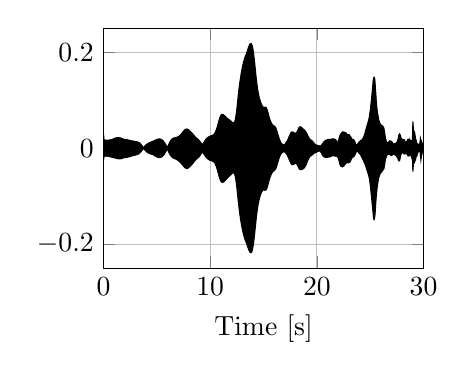
\begin{tikzpicture}

\begin{axis}[%
width=1.6in,
height=1.2in,
at={(0.758in,0.481in)},
scale only axis,
xmin=0,
xmax=30,
xmajorgrids,
ymin=-0.25,
ymax=0.25,
ymajorgrids,
xlabel={Time [s]},
axis background/.style={fill=white}
]
\addplot[fill=black,draw=black,forget plot] plot table[row sep=crcr]{%
2.08333333333333e-05	0.0289018154144287\\
0.0417454218822439	0.0172839164733887\\
0.0834700104311544	0.0172467231750488\\
0.125194598980065	0.0169233083724976\\
0.166919187528975	0.0168006420135498\\
0.208643776077886	0.0168346166610718\\
0.250368364626797	0.0167636871337891\\
0.292092953175707	0.0166480541229248\\
0.333817541724618	0.0166051387786865\\
0.375542130273528	0.0166434049606323\\
0.417266718822439	0.0166885852813721\\
0.458991307371349	0.0167794227600098\\
0.50071589592026	0.0168857574462891\\
0.54244048446917	0.0170364379882813\\
0.584165073018081	0.0171716213226318\\
0.625889661566991	0.0173765420913696\\
0.667614250115902	0.0174554586410522\\
0.709338838664812	0.0177245140075684\\
0.751063427213723	0.017983078956604\\
0.792788015762633	0.0181946754455566\\
0.834512604311544	0.0185127258300781\\
0.876237192860454	0.0188493728637695\\
0.917961781409365	0.0193003416061401\\
0.959686369958275	0.0198088884353638\\
1.00141095850719	0.0200985670089722\\
1.0431355470561	0.0205830335617065\\
1.08486013560501	0.0208804607391357\\
1.12658472415392	0.0212092399597168\\
1.16830931270283	0.0214753150939941\\
1.21003390125174	0.0217421054840088\\
1.25175848980065	0.021910548210144\\
1.29348307834956	0.0220106840133667\\
1.33520766689847	0.0220624208450317\\
1.37693225544738	0.0221121311187744\\
1.41865684399629	0.0220358371734619\\
1.4603814325452	0.0219392776489258\\
1.50210602109411	0.0216885805130005\\
1.54383060964302	0.0216819047927856\\
1.58555519819193	0.0215367078781128\\
1.62727978674084	0.021142840385437\\
1.66900437528975	0.020808219909668\\
1.71072896383866	0.020382285118103\\
1.75245355238758	0.0199680328369141\\
1.79417814093649	0.0196037292480469\\
1.8359027294854	0.0192145109176636\\
1.87762731803431	0.0189343690872192\\
1.91935190658322	0.0186411142349243\\
1.96107649513213	0.0184284448623657\\
2.00280108368104	0.0181646347045898\\
2.04452567222995	0.0180336236953735\\
2.08625026077886	0.0181005001068115\\
2.12797484932777	0.0181397199630737\\
2.16969943787668	0.0180549621582031\\
2.21142402642559	0.0176856517791748\\
2.2531486149745	0.017352819442749\\
2.29487320352341	0.0171602964401245\\
2.33659779207232	0.016951322555542\\
2.37832238062123	0.0167089700698853\\
2.42004696917014	0.0165107250213623\\
2.46177155771905	0.0162858963012695\\
2.50349614626796	0.0160504579544067\\
2.54522073481687	0.0158352851867676\\
2.58694532336579	0.015636682510376\\
2.6286699119147	0.0154330730438232\\
2.67039450046361	0.0152326822280884\\
2.71211908901252	0.0150892734527588\\
2.75384367756143	0.0149924755096436\\
2.79556826611034	0.0148319005966187\\
2.83729285465925	0.0146644115447998\\
2.87901744320816	0.0144762992858887\\
2.92074203175707	0.0142840147018433\\
2.96246662030598	0.0141104459762573\\
3.00419120885489	0.0139176845550537\\
3.0459157974038	0.0137656927108765\\
3.08764038595271	0.01357102394104\\
3.12936497450162	0.013383150100708\\
3.17108956305053	0.013142466545105\\
3.21281415159944	0.0128474235534668\\
3.25453874014835	0.0124889612197876\\
3.29626332869726	0.0120735168457031\\
3.33798791724618	0.0115724802017212\\
3.37971250579509	0.0108206272125244\\
3.421437094344	0.00982666015625\\
3.46316168289291	0.00880944728851318\\
3.50488627144182	0.00790166854858398\\
3.54661085999073	0.00679206848144531\\
3.58833544853964	0.00567448139190674\\
3.63006003708855	0.00451695919036865\\
3.67178462563746	0.00328445434570313\\
3.71350921418637	0.00202202796936035\\
3.75523380273528	0.00129556655883789\\
3.79695839128419	0.00241029262542725\\
3.8386829798331	0.00348067283630371\\
3.88040756838201	0.00458967685699463\\
3.92213215693092	0.00555455684661865\\
3.96385674547983	0.00644123554229736\\
4.00558133402874	0.00734257698059082\\
4.04730592257765	0.00802874565124512\\
4.08903051112656	0.00880241394042969\\
4.13075509967547	0.0093923807144165\\
4.17247968822439	0.0100157260894775\\
4.2142042767733	0.0106081962585449\\
4.25592886532221	0.0111130475997925\\
4.29765345387112	0.0115140676498413\\
4.33937804242003	0.0119895935058594\\
4.38110263096894	0.0123151540756226\\
4.42282721951785	0.0126434564590454\\
4.46455180806676	0.0130331516265869\\
4.50627639661567	0.0133864879608154\\
4.54800098516458	0.0137673616409302\\
4.58972557371349	0.0140365362167358\\
4.6314501622624	0.0143996477127075\\
4.67317475081131	0.0149127244949341\\
4.71489933936022	0.0153887271881104\\
4.75662392790913	0.0158339738845825\\
4.79834851645804	0.0162566900253296\\
4.84007310500695	0.0167093276977539\\
4.88179769355586	0.0170891284942627\\
4.92352228210478	0.017465353012085\\
4.96524687065368	0.0178946256637573\\
5.0069714592026	0.0182064771652222\\
5.04869604775151	0.0185272693634033\\
5.09042063630042	0.0188342332839966\\
5.13214522484933	0.0190325975418091\\
5.17386981339824	0.0192105770111084\\
5.21559440194715	0.0193079710006714\\
5.25731899049606	0.0192486047744751\\
5.29904357904497	0.0191446542739868\\
5.34076816759388	0.0189278125762939\\
5.38249275614279	0.0185902118682861\\
5.4242173446917	0.0181488990783691\\
5.46594193324061	0.0175989866256714\\
5.50766652178952	0.0168670415878296\\
5.54939111033843	0.0160067081451416\\
5.59111569888734	0.0151246786117554\\
5.63284028743625	0.0141278505325317\\
5.67456487598516	0.0128729343414307\\
5.71628946453407	0.0115524530410767\\
5.75801405308299	0.0100895166397095\\
5.7997386416319	0.0085594654083252\\
5.84146323018081	0.00689804553985596\\
5.88318781872972	0.00517868995666504\\
5.92491240727863	0.00329446792602539\\
5.96663699582754	0.00133967399597168\\
6.00836158437645	0.00280666351318359\\
6.05008617292536	0.00491511821746826\\
6.09181076147427	0.00697481632232666\\
6.13353535002318	0.00899100303649902\\
6.17525993857209	0.0109190940856934\\
6.216984527121	0.0126893520355225\\
6.25870911566991	0.0144162178039551\\
6.30043370421882	0.0158151388168335\\
6.34215829276773	0.0170881748199463\\
6.38388288131664	0.0181125402450562\\
6.42560746986555	0.0189999341964722\\
6.46733205841446	0.0197155475616455\\
6.50905664696338	0.0202987194061279\\
6.55078123551229	0.0207911729812622\\
6.5925058240612	0.0212439298629761\\
6.63423041261011	0.0215213298797607\\
6.67595500115902	0.0217323303222656\\
6.71767958970793	0.0219781398773193\\
6.75940417825684	0.0222369432449341\\
6.80112876680575	0.022428035736084\\
6.84285335535466	0.0226520299911499\\
6.88457794390357	0.022971510887146\\
6.92630253245248	0.0232703685760498\\
6.96802712100139	0.0237196683883667\\
7.0097517095503	0.0242148637771606\\
7.05147629809921	0.0247970819473267\\
7.09320088664812	0.0253957509994507\\
7.13492547519703	0.0261216163635254\\
7.17665006374594	0.0269925594329834\\
7.21837465229485	0.0279058218002319\\
7.26009924084376	0.0288667678833008\\
7.30182382939268	0.0299468040466309\\
7.34354841794159	0.0310767889022827\\
7.3852730064905	0.0321928262710571\\
7.42699759503941	0.0334115028381348\\
7.46872218358832	0.0345094203948975\\
7.51044677213723	0.0356947183609009\\
7.55217136068614	0.0367645025253296\\
7.59389594923505	0.0378050804138184\\
7.63562053778396	0.0386360883712769\\
7.67734512633287	0.0392385721206665\\
7.71906971488178	0.0396881103515625\\
7.76079430343069	0.0399270057678223\\
7.8025188919796	0.0399570465087891\\
7.84424348052851	0.0398741960525513\\
7.88596806907742	0.0395873785018921\\
7.92769265762633	0.0390733480453491\\
7.96941724617524	0.0384289026260376\\
8.01114183472416	0.0376578569412231\\
8.05286642327307	0.0367749929428101\\
8.09459101182198	0.0358628034591675\\
8.13631560037089	0.0349060297012329\\
8.1780401889198	0.0339477062225342\\
8.21976477746871	0.0330482721328735\\
8.26148936601762	0.0320686101913452\\
8.30321395456653	0.0310971736907959\\
8.34493854311544	0.0300194025039673\\
8.38666313166435	0.0290623903274536\\
8.42838772021326	0.0279207229614258\\
8.47011230876217	0.0267906188964844\\
8.51183689731108	0.0257227420806885\\
8.55356148585999	0.0247180461883545\\
8.5952860744089	0.023669958114624\\
8.63701066295781	0.0226560831069946\\
8.67873525150672	0.0218380689620972\\
8.72045984005563	0.0209788084030151\\
8.76218442860454	0.0201468467712402\\
8.80390901715345	0.0193407535552979\\
8.84563360570237	0.0184930562973022\\
8.88735819425128	0.0177232027053833\\
8.92908278280018	0.0168216228485107\\
8.9708073713491	0.0157843828201294\\
9.01253195989801	0.0146199464797974\\
9.05425654844692	0.0133260488510132\\
9.09598113699583	0.0120087862014771\\
9.13770572554474	0.0106837749481201\\
9.17943031409365	0.00940942764282227\\
9.22115490264256	0.00850355625152588\\
9.26287949119147	0.00812435150146484\\
9.30460407974038	0.00876319408416748\\
9.34632866828929	0.0099722146987915\\
9.3880532568382	0.0113373994827271\\
9.42977784538711	0.012898325920105\\
9.47150243393602	0.0144829750061035\\
9.51322702248493	0.0158678293228149\\
9.55495161103384	0.0172642469406128\\
9.59667619958275	0.0185226202011108\\
9.63840078813166	0.0195076465606689\\
9.68012537668058	0.0205553770065308\\
9.72184996522949	0.0214090347290039\\
9.7635745537784	0.0221755504608154\\
9.80529914232731	0.022851824760437\\
9.84702373087622	0.0234831571578979\\
9.88874831942513	0.024012565612793\\
9.93047290797404	0.0245404243469238\\
9.97219749652295	0.0249526500701904\\
10.0139220850719	0.0253311395645142\\
10.0556466736208	0.0255968570709229\\
10.0973712621697	0.0260077714920044\\
10.1390958507186	0.0262694358825684\\
10.1808204392675	0.0266389846801758\\
10.2225450278164	0.0270633697509766\\
10.2642696163653	0.0275228023529053\\
10.3059942049142	0.028225302696228\\
10.3477187934631	0.0291279554367065\\
10.3894433820121	0.0302877426147461\\
10.431167970561	0.0315402746200562\\
10.4728925591099	0.0332167148590088\\
10.5146171476588	0.0351763963699341\\
10.5563417362077	0.0375477075576782\\
10.5980663247566	0.0401661396026611\\
10.6397909133055	0.0431238412857056\\
10.6815155018544	0.0461913347244263\\
10.7232400904033	0.049560546875\\
10.7649646789523	0.0530068874359131\\
10.8066892675012	0.0566960573196411\\
10.8484138560501	0.059739351272583\\
10.890138444599	0.0628664493560791\\
10.9318630331479	0.0654891729354858\\
10.9735876216968	0.0675809383392334\\
11.0153122102457	0.0690361261367798\\
11.0570367987946	0.0699958801269531\\
11.0987613873435	0.0704505443572998\\
11.1404859758924	0.0704613924026489\\
11.1822105644414	0.0703864097595215\\
11.2239351529903	0.069923996925354\\
11.2656597415392	0.0691846609115601\\
11.3073843300881	0.0681769847869873\\
11.349108918637	0.0675182342529297\\
11.3908335071859	0.0665948390960693\\
11.4325580957348	0.0656557083129883\\
11.4742826842837	0.0647404193878174\\
11.5160072728326	0.0638628005981445\\
11.5577318613816	0.062997579574585\\
11.5994564499305	0.0622282028198242\\
11.6411810384794	0.0615196228027344\\
11.6829056270283	0.0608476400375366\\
11.7246302155772	0.0601366758346558\\
11.7663548041261	0.059431791305542\\
11.808079392675	0.0587942600250244\\
11.8498039812239	0.0581710338592529\\
11.8915285697728	0.0573031902313232\\
11.9332531583217	0.0566179752349854\\
11.9749777468707	0.0556339025497437\\
12.0167023354196	0.0547635555267334\\
12.0584269239685	0.0539953708648682\\
12.1001515125174	0.0533024072647095\\
12.1418761010663	0.0527950525283813\\
12.1836006896152	0.0525704622268677\\
12.2253252781641	0.0528875589370728\\
12.267049866713	0.0539987087249756\\
12.3087744552619	0.0564165115356445\\
12.3504990438108	0.0596647262573242\\
12.3922236323598	0.0642099380493164\\
12.4339482209087	0.0707371234893799\\
12.4756728094576	0.0776119232177734\\
12.5173973980065	0.0861227512359619\\
12.5591219865554	0.0951486825942993\\
12.6008465751043	0.10431981086731\\
12.6425711636532	0.112886786460876\\
12.6842957522021	0.12097704410553\\
12.726020340751	0.128900766372681\\
12.7677449293	0.1358243227005\\
12.8094695178489	0.142127275466919\\
12.8511941063978	0.148015379905701\\
12.8929186949467	0.154236793518066\\
12.9346432834956	0.159685373306274\\
12.9763678720445	0.164813637733459\\
13.0180924605934	0.168889880180359\\
13.0598170491423	0.173381924629211\\
13.1015416376912	0.177098035812378\\
13.1432662262401	0.180888175964355\\
13.1849908147891	0.183996677398682\\
13.226715403338	0.187105059623718\\
13.2684399918869	0.190197110176086\\
13.3101645804358	0.192168951034546\\
13.3518891689847	0.194461584091187\\
13.3936137575336	0.196935892105103\\
13.4353383460825	0.199378848075867\\
13.4770629346314	0.202369451522827\\
13.5187875231803	0.205432295799255\\
13.5605121117293	0.208498239517212\\
13.6022367002782	0.210684061050415\\
13.6439612888271	0.213081836700439\\
13.685685877376	0.215790510177612\\
13.7274104659249	0.217055559158325\\
13.7691350544738	0.217786312103271\\
13.8108596430227	0.217901468276978\\
13.8525842315716	0.217658996582031\\
13.8943088201205	0.215701222419739\\
13.9360334086694	0.212946772575378\\
13.9777579972184	0.209533333778381\\
14.0194825857673	0.204362273216248\\
14.0612071743162	0.197532534599304\\
14.1029317628651	0.190032243728638\\
14.144656351414	0.182183027267456\\
14.1863809399629	0.173431515693665\\
14.2281055285118	0.16433048248291\\
14.2698301170607	0.154643177986145\\
14.3115547056096	0.145938038825989\\
14.3532792941586	0.137869119644165\\
14.3950038827075	0.130620121955872\\
14.4367284712564	0.124011516571045\\
14.4784530598053	0.118113040924072\\
14.5201776483542	0.113308310508728\\
14.5619022369031	0.109058856964111\\
14.603626825452	0.105234384536743\\
14.6453514140009	0.101621270179749\\
14.6870760025498	0.0985941886901855\\
14.7288005910988	0.0958116054534912\\
14.7705251796477	0.0933703184127808\\
14.8122497681966	0.0910696983337402\\
14.8539743567455	0.089099645614624\\
14.8956989452944	0.0875579118728638\\
14.9374235338433	0.0863792896270752\\
14.9791481223922	0.0855422019958496\\
15.0208727109411	0.0850588083267212\\
15.06259729949	0.0850603580474854\\
15.1043218880389	0.085296630859375\\
15.1460464765879	0.0855298042297363\\
15.1877710651368	0.0854051113128662\\
15.2294956536857	0.0849155187606812\\
15.2712202422346	0.0833410024642944\\
15.3129448307835	0.081504225730896\\
15.3546694193324	0.0788611173629761\\
15.3963940078813	0.0754616260528564\\
15.4381185964302	0.0722217559814453\\
15.4798431849791	0.0684236288070679\\
15.521567773528	0.0648130178451538\\
15.563292362077	0.0617462396621704\\
15.6050169506259	0.0590245723724365\\
15.6467415391748	0.0567018985748291\\
15.6884661277237	0.0544013977050781\\
15.7301907162726	0.0523393154144287\\
15.7719153048215	0.0509884357452393\\
15.8136398933704	0.0495656728744507\\
15.8553644819193	0.0485960245132446\\
15.8970890704682	0.0475773811340332\\
15.9388136590172	0.0471309423446655\\
15.9805382475661	0.0466775894165039\\
16.022262836115	0.0456027984619141\\
16.0639874246639	0.0449638366699219\\
16.1057120132128	0.0437217950820923\\
16.1474366017617	0.0421873331069946\\
16.1891611903106	0.0398157835006714\\
16.2308857788595	0.0370414257049561\\
16.2726103674084	0.0340933799743652\\
16.3143349559573	0.030846118927002\\
16.3560595445063	0.0276812314987183\\
16.3977841330552	0.0246642827987671\\
16.4395087216041	0.0216168165206909\\
16.481233310153	0.0190800428390503\\
16.5229578987019	0.0165292024612427\\
16.5646824872508	0.0145782232284546\\
16.6064070757997	0.0126596689224243\\
16.6481316643486	0.0109900236129761\\
16.6898562528975	0.0097583532333374\\
16.7315808414465	0.00895917415618896\\
16.7733054299954	0.00827789306640625\\
16.8150300185443	0.00766324996948242\\
16.8567546070932	0.00714516639709473\\
16.8984791956421	0.00706076622009277\\
16.940203784191	0.00699281692504883\\
16.9819283727399	0.00745880603790283\\
17.0236529612888	0.00892043113708496\\
17.0653775498377	0.0104683637619019\\
17.1071021383867	0.0118987560272217\\
17.1488267269356	0.0132825374603271\\
17.1905513154845	0.0147570371627808\\
17.2322759040334	0.0158190727233887\\
17.2740004925823	0.0179071426391602\\
17.3157250811312	0.0198122262954712\\
17.3574496696801	0.0222957134246826\\
17.399174258229	0.024295449256897\\
17.4408988467779	0.0264453887939453\\
17.4826234353268	0.0281827449798584\\
17.5243480238758	0.0302528142929077\\
17.5660726124247	0.0320953130722046\\
17.6077972009736	0.0331175327301025\\
17.6495217895225	0.0337903499603271\\
17.6912463780714	0.0339313745498657\\
17.7329709666203	0.0335948467254639\\
17.7746955551692	0.0331717729568481\\
17.8164201437181	0.0327168703079224\\
17.858144732267	0.0321707725524902\\
17.8998693208159	0.0316033363342285\\
17.9415939093649	0.0312644243240356\\
17.9833184979138	0.031225323677063\\
18.0250430864627	0.031514048576355\\
18.0667676750116	0.0324983596801758\\
18.1084922635605	0.0334329605102539\\
18.1502168521094	0.0346454381942749\\
18.1919414406583	0.0363898277282715\\
18.2336660292072	0.0386432409286499\\
18.2753906177561	0.0409408807754517\\
18.3171152063051	0.042599081993103\\
18.358839794854	0.0439639091491699\\
18.4005643834029	0.0444786548614502\\
18.4422889719518	0.0446840524673462\\
18.4840135605007	0.0445674657821655\\
18.5257381490496	0.0438816547393799\\
18.5674627375985	0.0431843996047974\\
18.6091873261474	0.0422766208648682\\
18.6509119146963	0.0414465665817261\\
18.6926365032453	0.0405653715133667\\
18.7343610917942	0.0396274328231812\\
18.7760856803431	0.038904070854187\\
18.817810268892	0.037988543510437\\
18.8595348574409	0.0374500751495361\\
18.9012594459898	0.0358611345291138\\
18.9429840345387	0.0345665216445923\\
18.9847086230876	0.0333881378173828\\
19.0264332116365	0.0317909717559814\\
19.0681578001854	0.0299602746963501\\
19.1098823887344	0.0280114412307739\\
19.1516069772833	0.0258997678756714\\
19.1933315658322	0.0238531827926636\\
19.2350561543811	0.0222935676574707\\
19.27678074293	0.0207890272140503\\
19.3185053314789	0.0196282863616943\\
19.3602299200278	0.0184078216552734\\
19.4019545085767	0.0177725553512573\\
19.4436790971256	0.0171433687210083\\
19.4854036856745	0.0163733959197998\\
19.5271282742235	0.015724778175354\\
19.5688528627724	0.0148919820785522\\
19.6105774513213	0.0140026807785034\\
19.6523020398702	0.0128467082977295\\
19.6940266284191	0.0117405652999878\\
19.735751216968	0.010372519493103\\
19.7774758055169	0.00920093059539795\\
19.8192003940658	0.00819897651672363\\
19.8609249826147	0.00752389430999756\\
19.9026495711637	0.00702130794525146\\
19.9443741597126	0.00664663314819336\\
19.9860987482615	0.00620102882385254\\
20.0278233368104	0.00596189498901367\\
20.0695479253593	0.00590932369232178\\
20.1112725139082	0.00578403472900391\\
20.1529971024571	0.00535440444946289\\
20.194721691006	0.00505363941192627\\
20.2364462795549	0.0049208402633667\\
20.2781708681038	0.00460708141326904\\
20.3198954566528	0.00454461574554443\\
20.3616200452017	0.00488710403442383\\
20.4033446337506	0.00553083419799805\\
20.4450692222995	0.0066683292388916\\
20.4867938108484	0.00809812545776367\\
20.5285183993973	0.00930774211883545\\
20.5702429879462	0.0106962919235229\\
20.6119675764951	0.011995792388916\\
20.653692165044	0.0131216049194336\\
20.695416753593	0.0142356157302856\\
20.7371413421419	0.0149523019790649\\
20.7788659306908	0.0156830549240112\\
20.8205905192397	0.0163005590438843\\
20.8623151077886	0.0167378187179565\\
20.9040396963375	0.0171627998352051\\
20.9457642848864	0.0173757076263428\\
20.9874888734353	0.0176352262496948\\
21.0292134619842	0.0178518295288086\\
21.0709380505331	0.0180354118347168\\
21.1126626390821	0.0183186531066895\\
21.154387227631	0.0184358358383179\\
21.1961118161799	0.0185097455978394\\
21.2378364047288	0.0185719728469849\\
21.2795609932777	0.0185713768005371\\
21.3212855818266	0.018660306930542\\
21.3630101703755	0.0188301801681519\\
21.4047347589244	0.0190684795379639\\
21.4464593474733	0.0193107128143311\\
21.4881839360223	0.0194258689880371\\
21.5299085245712	0.0194205045700073\\
21.5716331131201	0.0193763971328735\\
21.613357701669	0.019231915473938\\
21.6550822902179	0.0189168453216553\\
21.6968068787668	0.0184459686279297\\
21.7385314673157	0.0178109407424927\\
21.7802560558646	0.0169012546539307\\
21.8219806444135	0.015790581703186\\
21.8637052329624	0.0145639181137085\\
21.9054298215114	0.0127744674682617\\
21.9471544100603	0.0109992027282715\\
21.9888789986092	0.0119913816452026\\
22.0306035871581	0.0156203508377075\\
22.072328175707	0.0191564559936523\\
22.1140527642559	0.0229815244674683\\
22.1557773528048	0.0259648561477661\\
22.1975019413537	0.0281026363372803\\
22.2392265299026	0.0296872854232788\\
22.2809511184516	0.0307902097702026\\
22.3226757070005	0.0322165489196777\\
22.3644002955494	0.0331045389175415\\
22.4061248840983	0.033525824546814\\
22.4478494726472	0.0341571569442749\\
22.4895740611961	0.0338946580886841\\
22.531298649745	0.0327298641204834\\
22.5730232382939	0.0324540138244629\\
22.6147478268428	0.033271312713623\\
22.6564724153917	0.0315899848937988\\
22.6981970039407	0.0300452709197998\\
22.7399215924896	0.0314294099807739\\
22.7816461810385	0.03013014793396\\
22.8233707695874	0.029229998588562\\
22.8650953581363	0.0288237333297729\\
22.9068199466852	0.0283288955688477\\
22.9485445352341	0.0280765295028687\\
22.990269123783	0.0275962352752686\\
23.0319937123319	0.0278973579406738\\
23.0737183008809	0.0260312557220459\\
23.1154428894298	0.0252242088317871\\
23.1571674779787	0.0236279964447021\\
23.1988920665276	0.0228269100189209\\
23.2406166550765	0.0205123424530029\\
23.2823412436254	0.0189820528030396\\
23.3240658321743	0.0179396867752075\\
23.3657904207232	0.0180474519729614\\
23.4075150092721	0.0182417631149292\\
23.449239597821	0.0173059701919556\\
23.49096418637	0.0163581371307373\\
23.5326887749189	0.0146356821060181\\
23.5744133634678	0.0125703811645508\\
23.6161379520167	0.00920665264129639\\
23.6578625405656	0.00736701488494873\\
23.6995871291145	0.00450408458709717\\
23.7413117176634	0.00574696063995361\\
23.7830363062123	0.00787520408630371\\
23.8247608947612	0.00892877578735352\\
23.8664854833102	0.0103286504745483\\
23.9082100718591	0.0116684436798096\\
23.949934660408	0.0127644538879395\\
23.9916592489569	0.0136789083480835\\
24.0333838375058	0.0147483348846436\\
24.0751084260547	0.0154931545257568\\
24.1168330146036	0.0160554647445679\\
24.1585576031525	0.016614556312561\\
24.2002821917014	0.0174537897109985\\
24.2420067802503	0.0184100866317749\\
24.2837313687993	0.0194147825241089\\
24.3254559573482	0.0205755233764648\\
24.3671805458971	0.0225957632064819\\
24.408905134446	0.0246201753616333\\
24.4506297229949	0.0273855924606323\\
24.4923543115438	0.0305709838867188\\
24.5340789000927	0.0339202880859375\\
24.5758034886416	0.0368626117706299\\
24.6175280771905	0.0406008958816528\\
24.6592526657395	0.0432379245758057\\
24.7009772542884	0.0475165843963623\\
24.7427018428373	0.0494333505630493\\
24.7844264313862	0.0534987449645996\\
24.8261510199351	0.0562107563018799\\
24.867875608484	0.0598803758621216\\
24.9096001970329	0.0644762516021729\\
24.9513247855818	0.0705916881561279\\
24.9930493741307	0.0768003463745117\\
25.0347739626796	0.0850495100021362\\
25.0764985512286	0.0934610366821289\\
25.1182231397775	0.102080225944519\\
25.1599477283264	0.111679911613464\\
25.2016723168753	0.12195873260498\\
25.2433969054242	0.131803393363953\\
25.2851214939731	0.142210364341736\\
25.326846082522	0.146503806114197\\
25.3685706710709	0.147769927978516\\
25.4102952596198	0.14683210849762\\
25.4520198481687	0.137254118919373\\
25.4937444367177	0.122432231903076\\
25.5354690252666	0.109551906585693\\
25.5771936138155	0.0951443910598755\\
25.6189182023644	0.0850281715393066\\
25.6606427909133	0.0770364999771118\\
25.7023673794622	0.0712352991104126\\
25.7440919680111	0.0659774541854858\\
25.78581655656	0.0599316358566284\\
25.8275411451089	0.0568866729736328\\
25.8692657336579	0.0542335510253906\\
25.9109903222068	0.0520757436752319\\
25.9527149107557	0.0504512786865234\\
25.9944394993046	0.0491634607315063\\
26.0361640878535	0.0481152534484863\\
26.0778886764024	0.0472562313079834\\
26.1196132649513	0.0468728542327881\\
26.1613378535002	0.046356201171875\\
26.2030624420491	0.0450063943862915\\
26.2447870305981	0.0437877178192139\\
26.286511619147	0.0409526824951172\\
26.3282362076959	0.0362191200256348\\
26.3699607962448	0.0297123193740845\\
26.4116853847937	0.023409366607666\\
26.4534099733426	0.019061803817749\\
26.4951345618915	0.0155285596847534\\
26.5368591504404	0.0123026371002197\\
26.5785837389893	0.0110095739364624\\
26.6203083275383	0.0112423896789551\\
26.6620329160872	0.0117638111114502\\
26.7037575046361	0.0123709440231323\\
26.745482093185	0.0134620666503906\\
26.7872066817339	0.0142861604690552\\
26.8289312702828	0.0154225826263428\\
26.8706558588317	0.0151021480560303\\
26.9123804473806	0.0148561000823975\\
26.9541050359295	0.01445472240448\\
26.9958296244784	0.0140252113342285\\
27.0375542130274	0.0131319761276245\\
27.0792788015763	0.0116654634475708\\
27.1210033901252	0.00979530811309814\\
27.1627279786741	0.00838565826416016\\
27.204452567223	0.00881707668304443\\
27.2461771557719	0.0093456506729126\\
27.2879017443208	0.00927639007568359\\
27.3296263328697	0.00986099243164063\\
27.3713509214186	0.0103861093521118\\
27.4130755099675	0.0106728076934814\\
27.4548000985165	0.0112987756729126\\
27.4965246870654	0.0121774673461914\\
27.5382492756143	0.0139634609222412\\
27.5799738641632	0.0164190530776978\\
27.6216984527121	0.0203505754470825\\
27.663423041261	0.0249905586242676\\
27.7051476298099	0.0289018154144287\\
27.7468722183588	0.0298447608947754\\
27.7885968069077	0.0291091203689575\\
27.8303213954567	0.0252009630203247\\
27.8720459840056	0.0223077535629272\\
27.9137705725545	0.0206351280212402\\
27.9554951611034	0.0192619562149048\\
27.9972197496523	0.0184595584869385\\
28.0389443382012	0.0177617073059082\\
28.0806689267501	0.0177174806594849\\
28.122393515299	0.0177733898162842\\
28.1641181038479	0.0177394151687622\\
28.2058426923968	0.0172935724258423\\
28.2475672809458	0.0144679546356201\\
28.2892918694947	0.0127115249633789\\
28.3310164580436	0.0125396251678467\\
28.3727410465925	0.0127661228179932\\
28.4144656351414	0.0140732526779175\\
28.4561902236903	0.0150754451751709\\
28.4979148122392	0.0173780918121338\\
28.5396394007881	0.0187383890151978\\
28.581363989337	0.0183737277984619\\
28.623088577886	0.0161203145980835\\
28.6648131664349	0.0153638124465942\\
28.7065377549838	0.0183824300765991\\
28.7482623435327	0.014249324798584\\
28.7899869320816	0.0155762434005737\\
28.8317115206305	0.0158883333206177\\
28.8734361091794	0.0149469375610352\\
28.9151606977283	0.0150916576385498\\
28.9568852862772	0.0151647329330444\\
28.9986098748261	0.0557581186294556\\
29.0403344633751	0.0413410663604736\\
29.082059051924	0.0348759889602661\\
29.1237836404729	0.0307329893112183\\
29.1655082290218	0.0322949886322021\\
29.2072328175707	0.0267981290817261\\
29.2489574061196	0.0197196006774902\\
29.2906819946685	0.0172826051712036\\
29.3324065832174	0.0132230520248413\\
29.3741311717663	0.00993311405181885\\
29.4158557603153	0.00903809070587158\\
29.4575803488642	0.00888538360595703\\
29.4993049374131	0.00769555568695068\\
29.541029525962	0.00678014755249023\\
29.5827541145109	0.00769805908203125\\
29.6244787030598	0.00737214088439941\\
29.6662032916087	0.0122532844543457\\
29.7079278801576	0.0205073356628418\\
29.7496524687065	0.0169622898101807\\
29.7913770572554	0.0158277750015259\\
29.8331016458044	0.0128624439239502\\
29.8748262343533	0.0103393793106079\\
29.9165508229022	0.00627219676971436\\
29.9582754114511	0.00435507297515869\\
30	0.00299990177154541\\
}
\closedcycle;
\addplot[fill=black,draw=black,forget plot] plot table[row sep=crcr]{%
2.08333333333333e-05	-0.0246125459671021\\
0.0417454218822439	-0.0171957015991211\\
0.0834700104311544	-0.0168211460113525\\
0.125194598980065	-0.0165849924087524\\
0.166919187528975	-0.0165097713470459\\
0.208643776077886	-0.0165896415710449\\
0.250368364626797	-0.0165733098983765\\
0.292092953175707	-0.0166329145431519\\
0.333817541724618	-0.0165641307830811\\
0.375542130273528	-0.0162385702133179\\
0.417266718822439	-0.0163146257400513\\
0.458991307371349	-0.0170029401779175\\
0.50071589592026	-0.0172367095947266\\
0.54244048446917	-0.017336368560791\\
0.584165073018081	-0.0175758600234985\\
0.625889661566991	-0.0178658962249756\\
0.667614250115902	-0.0180532932281494\\
0.709338838664812	-0.0183048248291016\\
0.751063427213723	-0.0185542106628418\\
0.792788015762633	-0.0187641382217407\\
0.834512604311544	-0.0190104246139526\\
0.876237192860454	-0.0192594528198242\\
0.917961781409365	-0.0194554328918457\\
0.959686369958275	-0.0197291374206543\\
1.00141095850719	-0.0200408697128296\\
1.0431355470561	-0.0202594995498657\\
1.08486013560501	-0.0204477310180664\\
1.12658472415392	-0.020601749420166\\
1.16830931270283	-0.0208448171615601\\
1.21003390125174	-0.0211573839187622\\
1.25175848980065	-0.0213598012924194\\
1.29348307834956	-0.0215791463851929\\
1.33520766689847	-0.021764874458313\\
1.37693225544738	-0.0218576192855835\\
1.41865684399629	-0.0219939947128296\\
1.4603814325452	-0.0221278667449951\\
1.50210602109411	-0.0222222805023193\\
1.54383060964302	-0.0221813917160034\\
1.58555519819193	-0.0219743251800537\\
1.62727978674084	-0.021693229675293\\
1.66900437528975	-0.0215275287628174\\
1.71072896383866	-0.0213046073913574\\
1.75245355238758	-0.0209816694259644\\
1.79417814093649	-0.0206918716430664\\
1.8359027294854	-0.0203981399536133\\
1.87762731803431	-0.0201077461242676\\
1.91935190658322	-0.0198572874069214\\
1.96107649513213	-0.0196220874786377\\
2.00280108368104	-0.0194137096405029\\
2.04452567222995	-0.0192828178405762\\
2.08625026077886	-0.0193582773208618\\
2.12797484932777	-0.0194087028503418\\
2.16969943787668	-0.0192368030548096\\
2.21142402642559	-0.0188260078430176\\
2.2531486149745	-0.0185443162918091\\
2.29487320352341	-0.0183073282241821\\
2.33659779207232	-0.0180861949920654\\
2.37832238062123	-0.0178505182266235\\
2.42004696917014	-0.0175933837890625\\
2.46177155771905	-0.0173068046569824\\
2.50349614626796	-0.0170255899429321\\
2.54522073481687	-0.0167592763900757\\
2.58694532336579	-0.0164722204208374\\
2.6286699119147	-0.0162140130996704\\
2.67039450046361	-0.015958309173584\\
2.71211908901252	-0.0157243013381958\\
2.75384367756143	-0.0154241323471069\\
2.79556826611034	-0.0152739286422729\\
2.83729285465925	-0.0150983333587646\\
2.87901744320816	-0.0148491859436035\\
2.92074203175707	-0.0145643949508667\\
2.96246662030598	-0.0143306255340576\\
3.00419120885489	-0.0140978097915649\\
3.0459157974038	-0.0138612985610962\\
3.08764038595271	-0.0136064291000366\\
3.12936497450162	-0.0132995843887329\\
3.17108956305053	-0.0129354000091553\\
3.21281415159944	-0.0125194787979126\\
3.25453874014835	-0.0120671987533569\\
3.29626332869726	-0.011597752571106\\
3.33798791724618	-0.0110057592391968\\
3.37971250579509	-0.0102317333221436\\
3.421437094344	-0.0091327428817749\\
3.46316168289291	-0.00810348987579346\\
3.50488627144182	-0.00718438625335693\\
3.54661085999073	-0.00608158111572266\\
3.58833544853964	-0.00491714477539063\\
3.63006003708855	-0.00370383262634277\\
3.67178462563746	-0.00244414806365967\\
3.71350921418637	-0.00149321556091309\\
3.75523380273528	-0.000998377799987793\\
3.79695839128419	-0.00172770023345947\\
3.8386829798331	-0.00276744365692139\\
3.88040756838201	-0.0038759708404541\\
3.92213215693092	-0.00488531589508057\\
3.96385674547983	-0.00586926937103271\\
4.00558133402874	-0.00676000118255615\\
4.04730592257765	-0.00754845142364502\\
4.08903051112656	-0.00828826427459717\\
4.13075509967547	-0.0089336633682251\\
4.17247968822439	-0.00953006744384766\\
4.2142042767733	-0.010079026222229\\
4.25592886532221	-0.010554313659668\\
4.29765345387112	-0.0109732151031494\\
4.33937804242003	-0.0113677978515625\\
4.38110263096894	-0.0116798877716064\\
4.42282721951785	-0.0120236873626709\\
4.46455180806676	-0.0122873783111572\\
4.50627639661567	-0.0126049518585205\\
4.54800098516458	-0.0129153728485107\\
4.58972557371349	-0.0131666660308838\\
4.6314501622624	-0.0134896039962769\\
4.67317475081131	-0.013935923576355\\
4.71489933936022	-0.0144619941711426\\
4.75662392790913	-0.0149557590484619\\
4.79834851645804	-0.0154992341995239\\
4.84007310500695	-0.0160280466079712\\
4.88179769355586	-0.0165845155715942\\
4.92352228210478	-0.0171357393264771\\
4.96524687065368	-0.0177779197692871\\
5.0069714592026	-0.0181328058242798\\
5.04869604775151	-0.0186460018157959\\
5.09042063630042	-0.0190161466598511\\
5.13214522484933	-0.0193103551864624\\
5.17386981339824	-0.0194894075393677\\
5.21559440194715	-0.0195547342300415\\
5.25731899049606	-0.0195143222808838\\
5.29904357904497	-0.0193486213684082\\
5.34076816759388	-0.0190967321395874\\
5.38249275614279	-0.018696665763855\\
5.4242173446917	-0.0182639360427856\\
5.46594193324061	-0.0176519155502319\\
5.50766652178952	-0.0169194936752319\\
5.54939111033843	-0.0160806179046631\\
5.59111569888734	-0.0152089595794678\\
5.63284028743625	-0.0141507387161255\\
5.67456487598516	-0.0129867792129517\\
5.71628946453407	-0.0116287469863892\\
5.75801405308299	-0.0101879835128784\\
5.7997386416319	-0.00864505767822266\\
5.84146323018081	-0.0070035457611084\\
5.88318781872972	-0.00519192218780518\\
5.92491240727863	-0.00336110591888428\\
5.96663699582754	-0.00136888027191162\\
6.00836158437645	-0.00284016132354736\\
6.05008617292536	-0.00491070747375488\\
6.09181076147427	-0.00699949264526367\\
6.13353535002318	-0.00890672206878662\\
6.17525993857209	-0.0108143091201782\\
6.216984527121	-0.0125757455825806\\
6.25870911566991	-0.0141395330429077\\
6.30043370421882	-0.0155307054519653\\
6.34215829276773	-0.0167557001113892\\
6.38388288131664	-0.0178036689758301\\
6.42560746986555	-0.0186706781387329\\
6.46733205841446	-0.0193828344345093\\
6.50905664696338	-0.0200213193893433\\
6.55078123551229	-0.0205178260803223\\
6.5925058240612	-0.0209612846374512\\
6.63423041261011	-0.0213786363601685\\
6.67595500115902	-0.0217491388320923\\
6.71767958970793	-0.0221091508865356\\
6.75940417825684	-0.0224461555480957\\
6.80112876680575	-0.0228430032730103\\
6.84285335535466	-0.0233157873153687\\
6.88457794390357	-0.023808479309082\\
6.92630253245248	-0.0244585275650024\\
6.96802712100139	-0.0251064300537109\\
7.0097517095503	-0.0258303880691528\\
7.05147629809921	-0.0265944004058838\\
7.09320088664812	-0.0274592638015747\\
7.13492547519703	-0.0283714532852173\\
7.17665006374594	-0.0292963981628418\\
7.21837465229485	-0.0301529169082642\\
7.26009924084376	-0.0311222076416016\\
7.30182382939268	-0.0321601629257202\\
7.34354841794159	-0.0331507921218872\\
7.3852730064905	-0.0342530012130737\\
7.42699759503941	-0.0353893041610718\\
7.46872218358832	-0.0365458726882935\\
7.51044677213723	-0.0376389026641846\\
7.55217136068614	-0.0387662649154663\\
7.59389594923505	-0.0397167205810547\\
7.63562053778396	-0.0405738353729248\\
7.67734512633287	-0.0413256883621216\\
7.71906971488178	-0.0418003797531128\\
7.76079430343069	-0.0420536994934082\\
7.8025188919796	-0.042178750038147\\
7.84424348052851	-0.0421346426010132\\
7.88596806907742	-0.0418459177017212\\
7.92769265762633	-0.0413744449615479\\
7.96941724617524	-0.0407599210739136\\
8.01114183472416	-0.0399363040924072\\
8.05286642327307	-0.0390793085098267\\
8.09459101182198	-0.0381475687026978\\
8.13631560037089	-0.0371774435043335\\
8.1780401889198	-0.0361678600311279\\
8.21976477746871	-0.0351506471633911\\
8.26148936601762	-0.0341503620147705\\
8.30321395456653	-0.0331231355667114\\
8.34493854311544	-0.0320142507553101\\
8.38666313166435	-0.0309340953826904\\
8.42838772021326	-0.0297716856002808\\
8.47011230876217	-0.028645396232605\\
8.51183689731108	-0.0274604558944702\\
8.55356148585999	-0.0263001918792725\\
8.5952860744089	-0.0253226757049561\\
8.63701066295781	-0.0244206190109253\\
8.67873525150672	-0.0233937501907349\\
8.72045984005563	-0.0225886106491089\\
8.76218442860454	-0.0216755867004395\\
8.80390901715345	-0.0208369493484497\\
8.84563360570237	-0.0200512409210205\\
8.88735819425128	-0.0191718339920044\\
8.92908278280018	-0.0182193517684937\\
8.9708073713491	-0.0172332525253296\\
9.01253195989801	-0.0159264802932739\\
9.05425654844692	-0.0146937370300293\\
9.09598113699583	-0.0132242441177368\\
9.13770572554474	-0.0118651390075684\\
9.17943031409365	-0.0105521678924561\\
9.22115490264256	-0.00942146778106689\\
9.26287949119147	-0.00874006748199463\\
9.30460407974038	-0.00917160511016846\\
9.34632866828929	-0.0101336240768433\\
9.3880532568382	-0.011370062828064\\
9.42977784538711	-0.0128998756408691\\
9.47150243393602	-0.0143510103225708\\
9.51322702248493	-0.0157495737075806\\
9.55495161103384	-0.0170753002166748\\
9.59667619958275	-0.0182063579559326\\
9.63840078813166	-0.0193357467651367\\
9.68012537668058	-0.0203588008880615\\
9.72184996522949	-0.0212153196334839\\
9.7635745537784	-0.0219855308532715\\
9.80529914232731	-0.0227525234222412\\
9.84702373087622	-0.0234038829803467\\
9.88874831942513	-0.0239938497543335\\
9.93047290797404	-0.0245486497879028\\
9.97219749652295	-0.0250680446624756\\
10.0139220850719	-0.025330662727356\\
10.0556466736208	-0.0257105827331543\\
10.0973712621697	-0.0259732007980347\\
10.1390958507186	-0.026237964630127\\
10.1808204392675	-0.026502251625061\\
10.2225450278164	-0.0268087387084961\\
10.2642696163653	-0.0272126197814941\\
10.3059942049142	-0.027822732925415\\
10.3477187934631	-0.0287014245986938\\
10.3894433820121	-0.0296477079391479\\
10.431167970561	-0.0310862064361572\\
10.4728925591099	-0.0327365398406982\\
10.5146171476588	-0.0350370407104492\\
10.5563417362077	-0.0372680425643921\\
10.5980663247566	-0.04002845287323\\
10.6397909133055	-0.0428663492202759\\
10.6815155018544	-0.0462334156036377\\
10.7232400904033	-0.0496655702590942\\
10.7649646789523	-0.0530269145965576\\
10.8066892675012	-0.0566266775131226\\
10.8484138560501	-0.0599058866500854\\
10.890138444599	-0.062919020652771\\
10.9318630331479	-0.0655851364135742\\
10.9735876216968	-0.0677218437194824\\
11.0153122102457	-0.0692881345748901\\
11.0570367987946	-0.0703552961349487\\
11.0987613873435	-0.0708773136138916\\
11.1404859758924	-0.0709894895553589\\
11.1822105644414	-0.0709495544433594\\
11.2239351529903	-0.0706186294555664\\
11.2656597415392	-0.0700540542602539\\
11.3073843300881	-0.0692270994186401\\
11.349108918637	-0.0682432651519775\\
11.3908335071859	-0.0672953128814697\\
11.4325580957348	-0.0663257837295532\\
11.4742826842837	-0.065250039100647\\
11.5160072728326	-0.064250111579895\\
11.5577318613816	-0.0632681846618652\\
11.5994564499305	-0.0622355937957764\\
11.6411810384794	-0.0613340139389038\\
11.6829056270283	-0.0604349374771118\\
11.7246302155772	-0.0595695972442627\\
11.7663548041261	-0.058692455291748\\
11.808079392675	-0.0577574968338013\\
11.8498039812239	-0.0568913221359253\\
11.8915285697728	-0.0558986663818359\\
11.9332531583217	-0.0551501512527466\\
11.9749777468707	-0.0542042255401611\\
12.0167023354196	-0.0532376766204834\\
12.0584269239685	-0.0524978637695313\\
12.1001515125174	-0.0518068075180054\\
12.1418761010663	-0.0511271953582764\\
12.1836006896152	-0.0510300397872925\\
12.2253252781641	-0.0515639781951904\\
12.267049866713	-0.0529642105102539\\
12.3087744552619	-0.0555515289306641\\
12.3504990438108	-0.0588680505752563\\
12.3922236323598	-0.0639680624008179\\
12.4339482209087	-0.0703202486038208\\
12.4756728094576	-0.0782264471054077\\
12.5173973980065	-0.0863511562347412\\
12.5591219865554	-0.0954581499099731\\
12.6008465751043	-0.104357361793518\\
12.6425711636532	-0.113189697265625\\
12.6842957522021	-0.121339559555054\\
12.726020340751	-0.128985404968262\\
12.7677449293	-0.136216402053833\\
12.8094695178489	-0.142564058303833\\
12.8511941063978	-0.148672342300415\\
12.8929186949467	-0.154535055160522\\
12.9346432834956	-0.159825801849365\\
12.9763678720445	-0.1645427942276\\
13.0180924605934	-0.169322967529297\\
13.0598170491423	-0.173710465431213\\
13.1015416376912	-0.177278637886047\\
13.1432662262401	-0.181307435035706\\
13.1849908147891	-0.18419361114502\\
13.226715403338	-0.187656044960022\\
13.2684399918869	-0.190406203269959\\
13.3101645804358	-0.192665457725525\\
13.3518891689847	-0.195102095603943\\
13.3936137575336	-0.19741690158844\\
13.4353383460825	-0.199807286262512\\
13.4770629346314	-0.202930927276611\\
13.5187875231803	-0.205814123153687\\
13.5605121117293	-0.208544373512268\\
13.6022367002782	-0.210830450057983\\
13.6439612888271	-0.213446617126465\\
13.685685877376	-0.215301871299744\\
13.7274104659249	-0.216520667076111\\
13.7691350544738	-0.217375636100769\\
13.8108596430227	-0.217618823051453\\
13.8525842315716	-0.217018485069275\\
13.8943088201205	-0.215638637542725\\
13.9360334086694	-0.212983369827271\\
13.9777579972184	-0.20891547203064\\
14.0194825857673	-0.203665256500244\\
14.0612071743162	-0.197432398796082\\
14.1029317628651	-0.189883828163147\\
14.144656351414	-0.181927442550659\\
14.1863809399629	-0.173160552978516\\
14.2281055285118	-0.163904428482056\\
14.2698301170607	-0.155325651168823\\
14.3115547056096	-0.146464347839355\\
14.3532792941586	-0.138510823249817\\
14.3950038827075	-0.131142497062683\\
14.4367284712564	-0.124476313591003\\
14.4784530598053	-0.118629217147827\\
14.5201776483542	-0.113657116889954\\
14.5619022369031	-0.109098315238953\\
14.603626825452	-0.105221748352051\\
14.6453514140009	-0.101921081542969\\
14.6870760025498	-0.0989488363265991\\
14.7288005910988	-0.0962216854095459\\
14.7705251796477	-0.0939410924911499\\
14.8122497681966	-0.0917882919311523\\
14.8539743567455	-0.0903633832931519\\
14.8956989452944	-0.0887049436569214\\
14.9374235338433	-0.0874444246292114\\
14.9791481223922	-0.0868819952011108\\
15.0208727109411	-0.0866715908050537\\
15.06259729949	-0.0870622396469116\\
15.1043218880389	-0.0875006914138794\\
15.1460464765879	-0.0873923301696777\\
15.1877710651368	-0.0873476266860962\\
15.2294956536857	-0.0866729021072388\\
15.2712202422346	-0.0855406522750854\\
15.3129448307835	-0.0833112001419067\\
15.3546694193324	-0.0804721117019653\\
15.3963940078813	-0.0771454572677612\\
15.4381185964302	-0.0737349987030029\\
15.4798431849791	-0.0700196027755737\\
15.521567773528	-0.0666775703430176\\
15.563292362077	-0.0634448528289795\\
15.6050169506259	-0.0606918334960938\\
15.6467415391748	-0.0584330558776855\\
15.6884661277237	-0.0558235645294189\\
15.7301907162726	-0.0538029670715332\\
15.7719153048215	-0.0523076057434082\\
15.8136398933704	-0.0504846572875977\\
15.8553644819193	-0.0491800308227539\\
15.8970890704682	-0.0485423803329468\\
15.9388136590172	-0.0477427244186401\\
15.9805382475661	-0.0469673871994019\\
16.022262836115	-0.0462492704391479\\
16.0639874246639	-0.045426607131958\\
16.1057120132128	-0.0441824197769165\\
16.1474366017617	-0.0425839424133301\\
16.1891611903106	-0.0399463176727295\\
16.2308857788595	-0.0371644496917725\\
16.2726103674084	-0.0339317321777344\\
16.3143349559573	-0.0309123992919922\\
16.3560595445063	-0.0275505781173706\\
16.3977841330552	-0.0242971181869507\\
16.4395087216041	-0.0216097831726074\\
16.481233310153	-0.0191483497619629\\
16.5229578987019	-0.0166349411010742\\
16.5646824872508	-0.0146774053573608\\
16.6064070757997	-0.0128949880599976\\
16.6481316643486	-0.0113308429718018\\
16.6898562528975	-0.00998151302337646\\
16.7315808414465	-0.00920701026916504\\
16.7733054299954	-0.00858712196350098\\
16.8150300185443	-0.00793147087097168\\
16.8567546070932	-0.00783514976501465\\
16.8984791956421	-0.00753939151763916\\
16.940203784191	-0.00739538669586182\\
16.9819283727399	-0.00751733779907227\\
17.0236529612888	-0.0083467960357666\\
17.0653775498377	-0.00968194007873535\\
17.1071021383867	-0.0106027126312256\\
17.1488267269356	-0.0118948221206665\\
17.1905513154845	-0.0133209228515625\\
17.2322759040334	-0.0149599313735962\\
17.2740004925823	-0.0166279077529907\\
17.3157250811312	-0.0190941095352173\\
17.3574496696801	-0.0211161375045776\\
17.399174258229	-0.0233792066574097\\
17.4408988467779	-0.0254983901977539\\
17.4826234353268	-0.0276591777801514\\
17.5243480238758	-0.0296339988708496\\
17.5660726124247	-0.0314292907714844\\
17.6077972009736	-0.0327898263931274\\
17.6495217895225	-0.0339784622192383\\
17.6912463780714	-0.0342205762863159\\
17.7329709666203	-0.0340787172317505\\
17.7746955551692	-0.033890962600708\\
17.8164201437181	-0.0336030721664429\\
17.858144732267	-0.0330919027328491\\
17.8998693208159	-0.0324126482009888\\
17.9415939093649	-0.0321135520935059\\
17.9833184979138	-0.0316779613494873\\
18.0250430864627	-0.0319186449050903\\
18.0667676750116	-0.0325645208358765\\
18.1084922635605	-0.0331162214279175\\
18.1502168521094	-0.0341336727142334\\
18.1919414406583	-0.0357980728149414\\
18.2336660292072	-0.0379602909088135\\
18.2753906177561	-0.039898157119751\\
18.3171152063051	-0.0417532920837402\\
18.358839794854	-0.0432174205780029\\
18.4005643834029	-0.0439836978912354\\
18.4422889719518	-0.0446689128875732\\
18.4840135605007	-0.0447372198104858\\
18.5257381490496	-0.0446585416793823\\
18.5674627375985	-0.0444197654724121\\
18.6091873261474	-0.0438452959060669\\
18.6509119146963	-0.0434389114379883\\
18.6926365032453	-0.0431008338928223\\
18.7343610917942	-0.0425100326538086\\
18.7760856803431	-0.041858434677124\\
18.817810268892	-0.0409421920776367\\
18.8595348574409	-0.0395234823226929\\
18.9012594459898	-0.0379773378372192\\
18.9429840345387	-0.0363748073577881\\
18.9847086230876	-0.0346890687942505\\
19.0264332116365	-0.0323585271835327\\
19.0681578001854	-0.029951810836792\\
19.1098823887344	-0.0273469686508179\\
19.1516069772833	-0.0249150991439819\\
19.1933315658322	-0.0228530168533325\\
19.2350561543811	-0.0210275650024414\\
19.27678074293	-0.0195722579956055\\
19.3185053314789	-0.0182263851165771\\
19.3602299200278	-0.0170451402664185\\
19.4019545085767	-0.0163646936416626\\
19.4436790971256	-0.015835165977478\\
19.4854036856745	-0.0151834487915039\\
19.5271282742235	-0.0144050121307373\\
19.5688528627724	-0.0135834217071533\\
19.6105774513213	-0.0125962495803833\\
19.6523020398702	-0.0117663145065308\\
19.6940266284191	-0.0110212564468384\\
19.735751216968	-0.0102546215057373\\
19.7774758055169	-0.00987803936004639\\
19.8192003940658	-0.00958847999572754\\
19.8609249826147	-0.0093231201171875\\
19.9026495711637	-0.00883936882019043\\
19.9443741597126	-0.00836265087127686\\
19.9860987482615	-0.00787353515625\\
20.0278233368104	-0.00743007659912109\\
20.0695479253593	-0.00707113742828369\\
20.1112725139082	-0.00668859481811523\\
20.1529971024571	-0.00615251064300537\\
20.194721691006	-0.00586700439453125\\
20.2364462795549	-0.00560557842254639\\
20.2781708681038	-0.00583541393280029\\
20.3198954566528	-0.00655210018157959\\
20.3616200452017	-0.00776052474975586\\
20.4033446337506	-0.00930595397949219\\
20.4450692222995	-0.0109794139862061\\
20.4867938108484	-0.0127259492874146\\
20.5285183993973	-0.0143998861312866\\
20.5702429879462	-0.0158244371414185\\
20.6119675764951	-0.016818642616272\\
20.653692165044	-0.0178283452987671\\
20.695416753593	-0.0182756185531616\\
20.7371413421419	-0.0186376571655273\\
20.7788659306908	-0.0187970399856567\\
20.8205905192397	-0.0188976526260376\\
20.8623151077886	-0.0189497470855713\\
20.9040396963375	-0.0189293622970581\\
20.9457642848864	-0.0188652276992798\\
20.9874888734353	-0.0187562704086304\\
21.0292134619842	-0.0186918973922729\\
21.0709380505331	-0.0185267925262451\\
21.1126626390821	-0.0184204578399658\\
21.154387227631	-0.0182045698165894\\
21.1961118161799	-0.0180360078811646\\
21.2378364047288	-0.0177829265594482\\
21.2795609932777	-0.0173580646514893\\
21.3212855818266	-0.0168569087982178\\
21.3630101703755	-0.0163446664810181\\
21.4047347589244	-0.0159529447555542\\
21.4464593474733	-0.0156861543655396\\
21.4881839360223	-0.0156958103179932\\
21.5299085245712	-0.0157896280288696\\
21.5716331131201	-0.0159649848937988\\
21.613357701669	-0.0160847902297974\\
21.6550822902179	-0.0162127017974854\\
21.6968068787668	-0.0162982940673828\\
21.7385314673157	-0.0163229703903198\\
21.7802560558646	-0.0163854360580444\\
21.8219806444135	-0.0165865421295166\\
21.8637052329624	-0.0168144702911377\\
21.9054298215114	-0.0174007415771484\\
21.9471544100603	-0.0182710886001587\\
21.9888789986092	-0.0197792053222656\\
22.0306035871581	-0.0225802659988403\\
22.072328175707	-0.0257362127304077\\
22.1140527642559	-0.0297520160675049\\
22.1557773528048	-0.0334802865982056\\
22.1975019413537	-0.0358248949050903\\
22.2392265299026	-0.0371750593185425\\
22.2809511184516	-0.0378161668777466\\
22.3226757070005	-0.037787914276123\\
22.3644002955494	-0.0384975671768188\\
22.4061248840983	-0.0385605096817017\\
22.4478494726472	-0.0377620458602905\\
22.4895740611961	-0.0378817319869995\\
22.531298649745	-0.0370857715606689\\
22.5730232382939	-0.0354235172271729\\
22.6147478268428	-0.0346719026565552\\
22.6564724153917	-0.033119797706604\\
22.6981970039407	-0.0319575071334839\\
22.7399215924896	-0.031156063079834\\
22.7816461810385	-0.0308055877685547\\
22.8233707695874	-0.0301275253295898\\
22.8650953581363	-0.0299327373504639\\
22.9068199466852	-0.0288224220275879\\
22.9485445352341	-0.0279603004455566\\
22.990269123783	-0.0301216840744019\\
23.0319937123319	-0.0288829803466797\\
23.0737183008809	-0.029329776763916\\
23.1154428894298	-0.0272676944732666\\
23.1571674779787	-0.0269027948379517\\
23.1988920665276	-0.0237401723861694\\
23.2406166550765	-0.0218284130096436\\
23.2823412436254	-0.0196887254714966\\
23.3240658321743	-0.0194797515869141\\
23.3657904207232	-0.0191580057144165\\
23.4075150092721	-0.018082857131958\\
23.449239597821	-0.017486572265625\\
23.49096418637	-0.0168368816375732\\
23.5326887749189	-0.0148299932479858\\
23.5744133634678	-0.0132225751876831\\
23.6161379520167	-0.0112380981445313\\
23.6578625405656	-0.00927329063415527\\
23.6995871291145	-0.00729405879974365\\
23.7413117176634	-0.00541198253631592\\
23.7830363062123	-0.00585329532623291\\
23.8247608947612	-0.00705087184906006\\
23.8664854833102	-0.00790441036224365\\
23.9082100718591	-0.00922906398773193\\
23.949934660408	-0.0103915929794312\\
23.9916592489569	-0.0109869241714478\\
24.0333838375058	-0.0121647119522095\\
24.0751084260547	-0.0132350921630859\\
24.1168330146036	-0.0147824287414551\\
24.1585576031525	-0.0163712501525879\\
24.2002821917014	-0.0181419849395752\\
24.2420067802503	-0.0201568603515625\\
24.2837313687993	-0.0218386650085449\\
24.3254559573482	-0.0237191915512085\\
24.3671805458971	-0.0257766246795654\\
24.408905134446	-0.0281181335449219\\
24.4506297229949	-0.0299117565155029\\
24.4923543115438	-0.0322684049606323\\
24.5340789000927	-0.0348150730133057\\
24.5758034886416	-0.0367872714996338\\
24.6175280771905	-0.0401309728622437\\
24.6592526657395	-0.0432840585708618\\
24.7009772542884	-0.0461442470550537\\
24.7427018428373	-0.0492013692855835\\
24.7844264313862	-0.0515936613082886\\
24.8261510199351	-0.0546169281005859\\
24.867875608484	-0.0579276084899902\\
24.9096001970329	-0.0619652271270752\\
24.9513247855818	-0.067317008972168\\
24.9930493741307	-0.0744342803955078\\
25.0347739626796	-0.0828894376754761\\
25.0764985512286	-0.0921531915664673\\
25.1182231397775	-0.100879669189453\\
25.1599477283264	-0.110393881797791\\
25.2016723168753	-0.120309472084045\\
25.2433969054242	-0.129265308380127\\
25.2851214939731	-0.139405250549316\\
25.326846082522	-0.147391200065613\\
25.3685706710709	-0.148532748222351\\
25.4102952596198	-0.145278573036194\\
25.4520198481687	-0.137319445610046\\
25.4937444367177	-0.122897028923035\\
25.5354690252666	-0.109067440032959\\
25.5771936138155	-0.0973917245864868\\
25.6189182023644	-0.0877518653869629\\
25.6606427909133	-0.0797009468078613\\
25.7023673794622	-0.0740842819213867\\
25.7440919680111	-0.0671932697296143\\
25.78581655656	-0.0624446868896484\\
25.8275411451089	-0.0591715574264526\\
25.8692657336579	-0.0568753480911255\\
25.9109903222068	-0.0544530153274536\\
25.9527149107557	-0.0524581670761108\\
25.9944394993046	-0.0512186288833618\\
26.0361640878535	-0.0501887798309326\\
26.0778886764024	-0.0488712787628174\\
26.1196132649513	-0.0478014945983887\\
26.1613378535002	-0.0465813875198364\\
26.2030624420491	-0.0451600551605225\\
26.2447870305981	-0.0438297986984253\\
26.286511619147	-0.0420979261398315\\
26.3282362076959	-0.0370039939880371\\
26.3699607962448	-0.0315877199172974\\
26.4116853847937	-0.024503231048584\\
26.4534099733426	-0.0207496881484985\\
26.4951345618915	-0.0188088417053223\\
26.5368591504404	-0.0155748128890991\\
26.5785837389893	-0.0144804716110229\\
26.6203083275383	-0.0133956670761108\\
26.6620329160872	-0.0126655101776123\\
26.7037575046361	-0.0126446485519409\\
26.745482093185	-0.0120810270309448\\
26.7872066817339	-0.0119867324829102\\
26.8289312702828	-0.012476921081543\\
26.8706558588317	-0.0136348009109497\\
26.9123804473806	-0.0146403312683105\\
26.9541050359295	-0.0152415037155151\\
26.9958296244784	-0.0153316259384155\\
27.0375542130274	-0.0147521495819092\\
27.0792788015763	-0.0136164426803589\\
27.1210033901252	-0.0125352144241333\\
27.1627279786741	-0.01247239112854\\
27.204452567223	-0.0130126476287842\\
27.2461771557719	-0.0132184028625488\\
27.2879017443208	-0.0135855674743652\\
27.3296263328697	-0.0140535831451416\\
27.3713509214186	-0.0145078897476196\\
27.4130755099675	-0.0152105093002319\\
27.4548000985165	-0.0161898136138916\\
27.4965246870654	-0.0174933671951294\\
27.5382492756143	-0.0185326337814331\\
27.5799738641632	-0.0206304788589478\\
27.6216984527121	-0.0230257511138916\\
27.663423041261	-0.0256621837615967\\
27.7051476298099	-0.0265785455703735\\
27.7468722183588	-0.0262367725372314\\
27.7885968069077	-0.0225502252578735\\
27.8303213954567	-0.0164459943771362\\
27.8720459840056	-0.013420581817627\\
27.9137705725545	-0.0112757682800293\\
27.9554951611034	-0.0101945400238037\\
27.9972197496523	-0.00948786735534668\\
28.0389443382012	-0.00926923751831055\\
28.0806689267501	-0.0095984935760498\\
28.122393515299	-0.0107908248901367\\
28.1641181038479	-0.011711597442627\\
28.2058426923968	-0.0124005079269409\\
28.2475672809458	-0.0123291015625\\
28.2892918694947	-0.0111650228500366\\
28.3310164580436	-0.0107495784759521\\
28.3727410465925	-0.0109363794326782\\
28.4144656351414	-0.0113959312438965\\
28.4561902236903	-0.0127084255218506\\
28.4979148122392	-0.0143774747848511\\
28.5396394007881	-0.0156912803649902\\
28.581363989337	-0.016010046005249\\
28.623088577886	-0.0150570869445801\\
28.6648131664349	-0.0156574249267578\\
28.7065377549838	-0.0146673917770386\\
28.7482623435327	-0.0125733613967896\\
28.7899869320816	-0.014132022857666\\
28.8317115206305	-0.0151126384735107\\
28.8734361091794	-0.0185130834579468\\
28.9151606977283	-0.0154259204864502\\
28.9568852862772	-0.0164726972579956\\
28.9986098748261	-0.0487018823623657\\
29.0403344633751	-0.0351096391677856\\
29.082059051924	-0.0307989120483398\\
29.1237836404729	-0.0304608345031738\\
29.1655082290218	-0.0294137001037598\\
29.2072328175707	-0.0246983766555786\\
29.2489574061196	-0.0243258476257324\\
29.2906819946685	-0.0183138847351074\\
29.3324065832174	-0.0172263383865356\\
29.3741311717663	-0.01677405834198\\
29.4158557603153	-0.0112394094467163\\
29.4575803488642	-0.00821816921234131\\
29.4993049374131	-0.00837206840515137\\
29.541029525962	-0.00689601898193359\\
29.5827541145109	-0.00672066211700439\\
29.6244787030598	-0.00574994087219238\\
29.6662032916087	-0.00678205490112305\\
29.7079278801576	-0.0144611597061157\\
29.7496524687065	-0.0238118171691895\\
29.7913770572554	-0.0168277025222778\\
29.8331016458044	-0.0137107372283936\\
29.8748262343533	-0.00925254821777344\\
29.9165508229022	-0.00644195079803467\\
29.9582754114511	-0.00364995002746582\\
30	-0.00271034240722656\\
}
\closedcycle;
\end{axis}
\end{tikzpicture}%
	\caption{Vibration from enclosure.}
	\label{fig:raw_enclosure19}
\end{subfigure}
\begin{subfigure}[t]{0.3\textwidth}
	\tikzsetnextfilename{Raw_microphone19}
	% This file was created by matlab2tikz.
%
%The latest updates can be retrieved from
%  http://www.mathworks.com/matlabcentral/fileexchange/22022-matlab2tikz-matlab2tikz
%where you can also make suggestions and rate matlab2tikz.
%
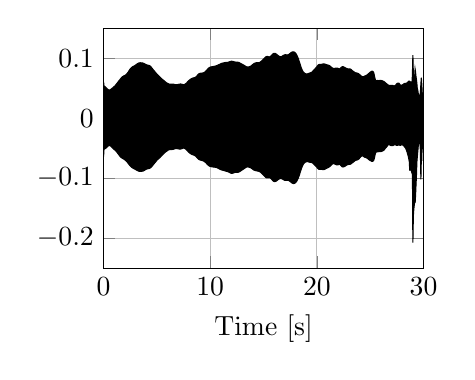
\begin{tikzpicture}

\begin{axis}[%
width=1.6in,
height=1.2in,
at={(0.758in,0.481in)},
scale only axis,
xmin=0,
xmax=30,
xmajorgrids,
ymin=-0.25,
ymax=0.15,
ymajorgrids,
xlabel={Time [s]},
axis background/.style={fill=white}
]
\addplot[fill=black,draw=black,forget plot] plot table[row sep=crcr]{%
2.08333333333333e-05	0.0603897571563721\\
0.0417454218822439	0.0536437034606934\\
0.0834700104311544	0.053246021270752\\
0.125194598980065	0.0526539087295532\\
0.166919187528975	0.0519295930862427\\
0.208643776077886	0.0513132810592651\\
0.250368364626797	0.0506181716918945\\
0.292092953175707	0.049962043762207\\
0.333817541724618	0.0491628646850586\\
0.375542130273528	0.0484598875045776\\
0.417266718822439	0.0478475093841553\\
0.458991307371349	0.0473896265029907\\
0.50071589592026	0.0470714569091797\\
0.54244048446917	0.0469733476638794\\
0.584165073018081	0.0470908880233765\\
0.625889661566991	0.0474280118942261\\
0.667614250115902	0.0478403568267822\\
0.709338838664812	0.0484753847122192\\
0.751063427213723	0.0490328073501587\\
0.792788015762633	0.0496945381164551\\
0.834512604311544	0.0502790212631226\\
0.876237192860454	0.0509083271026611\\
0.917961781409365	0.0515148639678955\\
0.959686369958275	0.0521837472915649\\
1.00141095850719	0.0528551340103149\\
1.0431355470561	0.0535385608673096\\
1.08486013560501	0.0542862415313721\\
1.12658472415392	0.0551106929779053\\
1.16830931270283	0.0561099052429199\\
1.21003390125174	0.0569859743118286\\
1.25175848980065	0.0579652786254883\\
1.29348307834956	0.0589110851287842\\
1.33520766689847	0.0598865747451782\\
1.37693225544738	0.0608971118927002\\
1.41865684399629	0.0619086027145386\\
1.4603814325452	0.0629016160964966\\
1.50210602109411	0.0636985301971436\\
1.54383060964302	0.0645028352737427\\
1.58555519819193	0.0655531883239746\\
1.62727978674084	0.0663880109786987\\
1.66900437528975	0.0673863887786865\\
1.71072896383866	0.0681266784667969\\
1.75245355238758	0.0687907934188843\\
1.79417814093649	0.0694630146026611\\
1.8359027294854	0.0697855949401855\\
1.87762731803431	0.0702035427093506\\
1.91935190658322	0.0707696676254272\\
1.96107649513213	0.0709508657455444\\
2.00280108368104	0.0712741613388062\\
2.04452567222995	0.0717693567276001\\
2.08625026077886	0.0723347663879395\\
2.12797484932777	0.073027491569519\\
2.16969943787668	0.0737733840942383\\
2.21142402642559	0.0745724439620972\\
2.2531486149745	0.0755566358566284\\
2.29487320352341	0.0765200853347778\\
2.33659779207232	0.0776286125183105\\
2.37832238062123	0.078802227973938\\
2.42004696917014	0.0800098180770874\\
2.46177155771905	0.0810554027557373\\
2.50349614626796	0.0821343660354614\\
2.54522073481687	0.0831148624420166\\
2.58694532336579	0.0838549137115479\\
2.6286699119147	0.0846198797225952\\
2.67039450046361	0.0851563215255737\\
2.71211908901252	0.085533618927002\\
2.75384367756143	0.0860351324081421\\
2.79556826611034	0.0864489078521729\\
2.83729285465925	0.0868340730667114\\
2.87901744320816	0.0872344970703125\\
2.92074203175707	0.0876197814941406\\
2.96246662030598	0.0881041288375854\\
3.00419120885489	0.0885660648345947\\
3.0459157974038	0.0891729593276978\\
3.08764038595271	0.0898017883300781\\
3.12936497450162	0.090296745300293\\
3.17108956305053	0.0907948017120361\\
3.21281415159944	0.0911823511123657\\
3.25453874014835	0.0915720462799072\\
3.29626332869726	0.0919393301010132\\
3.33798791724618	0.0921686887741089\\
3.37971250579509	0.0923402309417725\\
3.421437094344	0.0924153327941895\\
3.46316168289291	0.0923789739608765\\
3.50488627144182	0.0923339128494263\\
3.54661085999073	0.0922744274139404\\
3.58833544853964	0.0922480821609497\\
3.63006003708855	0.092125415802002\\
3.67178462563746	0.0919826030731201\\
3.71350921418637	0.091717004776001\\
3.75523380273528	0.0914278030395508\\
3.79695839128419	0.0910952091217041\\
3.8386829798331	0.0907164812088013\\
3.88040756838201	0.0903149843215942\\
3.92213215693092	0.0898522138595581\\
3.96385674547983	0.0893774032592773\\
4.00558133402874	0.0891425609588623\\
4.04730592257765	0.0888671875\\
4.08903051112656	0.0887078046798706\\
4.13075509967547	0.0885493755340576\\
4.17247968822439	0.0883456468582153\\
4.2142042767733	0.0881296396255493\\
4.25592886532221	0.0879220962524414\\
4.29765345387112	0.0875846147537231\\
4.33937804242003	0.0873188972473145\\
4.38110263096894	0.0867469310760498\\
4.42282721951785	0.0859829187393188\\
4.46455180806676	0.0852065086364746\\
4.50627639661567	0.0840591192245483\\
4.54800098516458	0.0832324028015137\\
4.58972557371349	0.0823162794113159\\
4.6314501622624	0.0813775062561035\\
4.67317475081131	0.080440878868103\\
4.71489933936022	0.0794827938079834\\
4.75662392790913	0.0786967277526855\\
4.79834851645804	0.0778450965881348\\
4.84007310500695	0.0770299434661865\\
4.88179769355586	0.0760402679443359\\
4.92352228210478	0.0751405954360962\\
4.96524687065368	0.0741815567016602\\
5.0069714592026	0.0734634399414063\\
5.04869604775151	0.0727047920227051\\
5.09042063630042	0.071963906288147\\
5.13214522484933	0.0712145566940308\\
5.17386981339824	0.0705695152282715\\
5.21559440194715	0.0698360204696655\\
5.25731899049606	0.0691730976104736\\
5.29904357904497	0.0684804916381836\\
5.34076816759388	0.0676901340484619\\
5.38249275614279	0.0669265985488892\\
5.4242173446917	0.0661585330963135\\
5.46594193324061	0.0654884576797485\\
5.50766652178952	0.0648449659347534\\
5.54939111033843	0.0641891956329346\\
5.59111569888734	0.0636188983917236\\
5.63284028743625	0.0629817247390747\\
5.67456487598516	0.0623445510864258\\
5.71628946453407	0.0617520809173584\\
5.75801405308299	0.0610983371734619\\
5.7997386416319	0.060491681098938\\
5.84146323018081	0.0599434375762939\\
5.88318781872972	0.0593322515487671\\
5.92491240727863	0.0588432550430298\\
5.96663699582754	0.0584088563919067\\
6.00836158437645	0.0580137968063354\\
6.05008617292536	0.0576294660568237\\
6.09181076147427	0.0572980642318726\\
6.13353535002318	0.0569523572921753\\
6.17525993857209	0.0568053722381592\\
6.216984527121	0.0568341016769409\\
6.25870911566991	0.0568625926971436\\
6.30043370421882	0.056931734085083\\
6.34215829276773	0.0569330453872681\\
6.38388288131664	0.0569413900375366\\
6.42560746986555	0.0569392442703247\\
6.46733205841446	0.0568947792053223\\
6.50905664696338	0.0568462610244751\\
6.55078123551229	0.0567140579223633\\
6.5925058240612	0.0564819574356079\\
6.63423041261011	0.0563000440597534\\
6.67595500115902	0.0561270713806152\\
6.71767958970793	0.0560063123703003\\
6.75940417825684	0.0558978319168091\\
6.80112876680575	0.0558294057846069\\
6.84285335535466	0.055874228477478\\
6.88457794390357	0.0559746026992798\\
6.92630253245248	0.0559996366500854\\
6.96802712100139	0.0562530755996704\\
7.0097517095503	0.0564032793045044\\
7.05147629809921	0.0565779209136963\\
7.09320088664812	0.0567010641098022\\
7.13492547519703	0.0568240880966187\\
7.17665006374594	0.0569539070129395\\
7.21837465229485	0.056983470916748\\
7.26009924084376	0.0569080114364624\\
7.30182382939268	0.0567911863327026\\
7.34354841794159	0.0565617084503174\\
7.3852730064905	0.0563559532165527\\
7.42699759503941	0.0561574697494507\\
7.46872218358832	0.0559893846511841\\
7.51044677213723	0.0559341907501221\\
7.55217136068614	0.056023120880127\\
7.59389594923505	0.05632483959198\\
7.63562053778396	0.0566648244857788\\
7.67734512633287	0.0572514533996582\\
7.71906971488178	0.0577679872512817\\
7.76079430343069	0.0583879947662354\\
7.8025188919796	0.058917760848999\\
7.84424348052851	0.0600001811981201\\
7.88596806907742	0.0608342885971069\\
7.92769265762633	0.0616427659988403\\
7.96941724617524	0.0623695850372314\\
8.01114183472416	0.0629762411117554\\
8.05286642327307	0.0635520219802856\\
8.09459101182198	0.0642280578613281\\
8.13631560037089	0.0647571086883545\\
8.1780401889198	0.065204381942749\\
8.21976477746871	0.0657062530517578\\
8.26148936601762	0.0660604238510132\\
8.30321395456653	0.0663700103759766\\
8.34493854311544	0.0667334794998169\\
8.38666313166435	0.0669504404067993\\
8.42838772021326	0.0672787427902222\\
8.47011230876217	0.0673421621322632\\
8.51183689731108	0.0675287246704102\\
8.55356148585999	0.0678279399871826\\
8.5952860744089	0.0681028366088867\\
8.63701066295781	0.0685756206512451\\
8.67873525150672	0.0691704750061035\\
8.72045984005563	0.069945216178894\\
8.76218442860454	0.0706884860992432\\
8.80390901715345	0.0715720653533936\\
8.84563360570237	0.0724829435348511\\
8.88735819425128	0.0732276439666748\\
8.92908278280018	0.0738719701766968\\
8.9708073713491	0.0742307901382446\\
9.01253195989801	0.0746057033538818\\
9.05425654844692	0.0747827291488647\\
9.09598113699583	0.0749812126159668\\
9.13770572554474	0.0750547647476196\\
9.17943031409365	0.0751036405563354\\
9.22115490264256	0.0751427412033081\\
9.26287949119147	0.0752674341201782\\
9.30460407974038	0.0753947496414185\\
9.34632866828929	0.0756101608276367\\
9.3880532568382	0.0758603811264038\\
9.42977784538711	0.0760928392410278\\
9.47150243393602	0.0765988826751709\\
9.51322702248493	0.0772473812103271\\
9.55495161103384	0.0779078006744385\\
9.59667619958275	0.0786309242248535\\
9.63840078813166	0.079386830329895\\
9.68012537668058	0.0802141427993774\\
9.72184996522949	0.0809791088104248\\
9.7635745537784	0.0818880796432495\\
9.80529914232731	0.0827025175094604\\
9.84702373087622	0.0834285020828247\\
9.88874831942513	0.0840182304382324\\
9.93047290797404	0.0844607353210449\\
9.97219749652295	0.0848827362060547\\
10.0139220850719	0.0851700305938721\\
10.0556466736208	0.0854588747024536\\
10.0973712621697	0.0856031179428101\\
10.1390958507186	0.0857107639312744\\
10.1808204392675	0.0858089923858643\\
10.2225450278164	0.0860016345977783\\
10.2642696163653	0.0861060619354248\\
10.3059942049142	0.0862765312194824\\
10.3477187934631	0.0864013433456421\\
10.3894433820121	0.0865577459335327\\
10.431167970561	0.0866743326187134\\
10.4728925591099	0.0868147611618042\\
10.5146171476588	0.0870430469512939\\
10.5563417362077	0.0872659683227539\\
10.5980663247566	0.0875405073165894\\
10.6397909133055	0.087854266166687\\
10.6815155018544	0.0879894495010376\\
10.7232400904033	0.0885801315307617\\
10.7649646789523	0.0889017581939697\\
10.8066892675012	0.0892288684844971\\
10.8484138560501	0.0895706415176392\\
10.890138444599	0.0899487733840942\\
10.9318630331479	0.0902535915374756\\
10.9735876216968	0.0906604528427124\\
11.0153122102457	0.0909847021102905\\
11.0570367987946	0.0912754535675049\\
11.0987613873435	0.091532826423645\\
11.1404859758924	0.0917465686798096\\
11.1822105644414	0.0918712615966797\\
11.2239351529903	0.0920858383178711\\
11.2656597415392	0.0921984910964966\\
11.3073843300881	0.0923914909362793\\
11.349108918637	0.092496395111084\\
11.3908335071859	0.0926185846328735\\
11.4325580957348	0.0927987098693848\\
11.4742826842837	0.0929298400878906\\
11.5160072728326	0.0929536819458008\\
11.5577318613816	0.0929762125015259\\
11.5994564499305	0.093025803565979\\
11.6411810384794	0.0931254625320435\\
11.6829056270283	0.0932999849319458\\
11.7246302155772	0.0935268402099609\\
11.7663548041261	0.0937992334365845\\
11.808079392675	0.0940710306167603\\
11.8498039812239	0.0943433046340942\\
11.8915285697728	0.0946346521377563\\
11.9332531583217	0.0948432683944702\\
11.9749777468707	0.0949058532714844\\
12.0167023354196	0.0949341058731079\\
12.0584269239685	0.0948581695556641\\
12.1001515125174	0.0947602987289429\\
12.1418761010663	0.094514012336731\\
12.1836006896152	0.0942853689193726\\
12.2253252781641	0.0940510034561157\\
12.267049866713	0.0938960313796997\\
12.3087744552619	0.0937067270278931\\
12.3504990438108	0.0936156511306763\\
12.3922236323598	0.0935498476028442\\
12.4339482209087	0.0935752391815186\\
12.4756728094576	0.0935707092285156\\
12.5173973980065	0.093549370765686\\
12.5591219865554	0.0934630632400513\\
12.6008465751043	0.0932536125183105\\
12.6425711636532	0.0930421352386475\\
12.6842957522021	0.0928412675857544\\
12.726020340751	0.0925585031509399\\
12.7677449293	0.0921374559402466\\
12.8094695178489	0.0916798114776611\\
12.8511941063978	0.0912390947341919\\
12.8929186949467	0.0908708572387695\\
12.9346432834956	0.0904514789581299\\
12.9763678720445	0.090067982673645\\
13.0180924605934	0.0896878242492676\\
13.0598170491423	0.0892894268035889\\
13.1015416376912	0.0887787342071533\\
13.1432662262401	0.0883601903915405\\
13.1849908147891	0.0879552364349365\\
13.226715403338	0.0875349044799805\\
13.2684399918869	0.0871306657791138\\
13.3101645804358	0.0866036415100098\\
13.3518891689847	0.0861753225326538\\
13.3936137575336	0.0856715440750122\\
13.4353383460825	0.0855777263641357\\
13.4770629346314	0.0854570865631104\\
13.5187875231803	0.0853261947631836\\
13.5605121117293	0.0852944850921631\\
13.6022367002782	0.0854312181472778\\
13.6439612888271	0.0856178998947144\\
13.685685877376	0.0858865976333618\\
13.7274104659249	0.0862277746200562\\
13.7691350544738	0.0865408182144165\\
13.8108596430227	0.0869563817977905\\
13.8525842315716	0.0874853134155273\\
13.8943088201205	0.0881596803665161\\
13.9360334086694	0.0887308120727539\\
13.9777579972184	0.0893298387527466\\
14.0194825857673	0.0899783372879028\\
14.0612071743162	0.0905156135559082\\
14.1029317628651	0.0910447835922241\\
14.144656351414	0.0914736986160278\\
14.1863809399629	0.0917195081710815\\
14.2281055285118	0.0919547080993652\\
14.2698301170607	0.0922614336013794\\
14.3115547056096	0.0923998355865479\\
14.3532792941586	0.0925300121307373\\
14.3950038827075	0.0925756692886353\\
14.4367284712564	0.0926344394683838\\
14.4784530598053	0.0926214456558228\\
14.5201776483542	0.092586874961853\\
14.5619022369031	0.0926744937896729\\
14.603626825452	0.092898964881897\\
14.6453514140009	0.0931074619293213\\
14.6870760025498	0.0934851169586182\\
14.7288005910988	0.0940217971801758\\
14.7705251796477	0.0946053266525269\\
14.8122497681966	0.0952993631362915\\
14.8539743567455	0.0960514545440674\\
14.8956989452944	0.0967358350753784\\
14.9374235338433	0.0974889993667603\\
14.9791481223922	0.0982786417007446\\
15.0208727109411	0.099073052406311\\
15.06259729949	0.0997766256332397\\
15.1043218880389	0.100573897361755\\
15.1460464765879	0.101248502731323\\
15.1877710651368	0.101884365081787\\
15.2294956536857	0.10239565372467\\
15.2712202422346	0.102736830711365\\
15.3129448307835	0.102862358093262\\
15.3546694193324	0.102890849113464\\
15.3963940078813	0.102792859077454\\
15.4381185964302	0.102585434913635\\
15.4798431849791	0.102324247360229\\
15.521567773528	0.102168202400208\\
15.563292362077	0.102325558662415\\
15.6050169506259	0.102575302124023\\
15.6467415391748	0.102971434593201\\
15.6884661277237	0.103570461273193\\
15.7301907162726	0.104301929473877\\
15.7719153048215	0.105123519897461\\
15.8136398933704	0.105985879898071\\
15.8553644819193	0.106854200363159\\
15.8970890704682	0.107379078865051\\
15.9388136590172	0.107751488685608\\
15.9805382475661	0.108096718788147\\
16.022262836115	0.108113765716553\\
16.0639874246639	0.108080387115479\\
16.1057120132128	0.10786247253418\\
16.1474366017617	0.107412338256836\\
16.1891611903106	0.106987714767456\\
16.2308857788595	0.106349587440491\\
16.2726103674084	0.105797648429871\\
16.3143349559573	0.10508120059967\\
16.3560595445063	0.104495167732239\\
16.3977841330552	0.103882908821106\\
16.4395087216041	0.103438138961792\\
16.481233310153	0.103041410446167\\
16.5229578987019	0.102787017822266\\
16.5646824872508	0.102577090263367\\
16.6064070757997	0.102519869804382\\
16.6481316643486	0.10261344909668\\
16.6898562528975	0.102864146232605\\
16.7315808414465	0.103113293647766\\
16.7733054299954	0.103682637214661\\
16.8150300185443	0.104214668273926\\
16.8567546070932	0.104674458503723\\
16.8984791956421	0.104979872703552\\
16.940203784191	0.105410099029541\\
16.9819283727399	0.105652809143066\\
17.0236529612888	0.105738043785095\\
17.0653775498377	0.105798125267029\\
17.1071021383867	0.105735182762146\\
17.1488267269356	0.105654954910278\\
17.1905513154845	0.105425596237183\\
17.2322759040334	0.105388879776001\\
17.2740004925823	0.10556697845459\\
17.3157250811312	0.105833888053894\\
17.3574496696801	0.10621190071106\\
17.399174258229	0.106717586517334\\
17.4408988467779	0.107341408729553\\
17.4826234353268	0.107905864715576\\
17.5243480238758	0.108482241630554\\
17.5660726124247	0.109076261520386\\
17.6077972009736	0.10957396030426\\
17.6495217895225	0.110042691230774\\
17.6912463780714	0.110330939292908\\
17.7329709666203	0.110543370246887\\
17.7746955551692	0.110642671585083\\
17.8164201437181	0.110597014427185\\
17.858144732267	0.110381841659546\\
17.8998693208159	0.109948396682739\\
17.9415939093649	0.109388828277588\\
17.9833184979138	0.108681201934814\\
18.0250430864627	0.107858061790466\\
18.0667676750116	0.106615900993347\\
18.1084922635605	0.105466723442078\\
18.1502168521094	0.103875517845154\\
18.1919414406583	0.102184891700745\\
18.2336660292072	0.100396633148193\\
18.2753906177561	0.0983184576034546\\
18.3171152063051	0.0960222482681274\\
18.358839794854	0.0938180685043335\\
18.4005643834029	0.091482400894165\\
18.4422889719518	0.0891180038452148\\
18.4840135605007	0.0867446660995483\\
18.5257381490496	0.0844603776931763\\
18.5674627375985	0.0824536085128784\\
18.6091873261474	0.0806264877319336\\
18.6509119146963	0.0791561603546143\\
18.6926365032453	0.0778614282608032\\
18.7343610917942	0.0768910646438599\\
18.7760856803431	0.0760853290557861\\
18.817810268892	0.0753868818283081\\
18.8595348574409	0.0748549699783325\\
18.9012594459898	0.0744881629943848\\
18.9429840345387	0.0741243362426758\\
18.9847086230876	0.0738319158554077\\
19.0264332116365	0.0737463235855103\\
19.0681578001854	0.0736725330352783\\
19.1098823887344	0.0738444328308105\\
19.1516069772833	0.0740232467651367\\
19.1933315658322	0.0743705034255981\\
19.2350561543811	0.0746517181396484\\
19.27678074293	0.0749346017837524\\
19.3185053314789	0.0752521753311157\\
19.3602299200278	0.0755175352096558\\
19.4019545085767	0.0757315158843994\\
19.4436790971256	0.0760165452957153\\
19.4854036856745	0.0763505697250366\\
19.5271282742235	0.0768413543701172\\
19.5688528627724	0.0773996114730835\\
19.6105774513213	0.078199028968811\\
19.6523020398702	0.0790597200393677\\
19.6940266284191	0.0797845125198364\\
19.735751216968	0.0806910991668701\\
19.7774758055169	0.0815376043319702\\
19.8192003940658	0.082292914390564\\
19.8609249826147	0.0830155611038208\\
19.9026495711637	0.0838862657546997\\
19.9443741597126	0.0847352743148804\\
19.9860987482615	0.0856231451034546\\
20.0278233368104	0.0866067409515381\\
20.0695479253593	0.0875283479690552\\
20.1112725139082	0.0884836912155151\\
20.1529971024571	0.0890350341796875\\
20.194721691006	0.0893949270248413\\
20.2364462795549	0.0895109176635742\\
20.2781708681038	0.0895265340805054\\
20.3198954566528	0.0895150899887085\\
20.3616200452017	0.0895940065383911\\
20.4033446337506	0.0896537303924561\\
20.4450692222995	0.089841365814209\\
20.4867938108484	0.0901130437850952\\
20.5285183993973	0.0902715921401978\\
20.5702429879462	0.0904438495635986\\
20.6119675764951	0.0905344486236572\\
20.653692165044	0.0905164480209351\\
20.695416753593	0.0904563665390015\\
20.7371413421419	0.0901918411254883\\
20.7788659306908	0.0900024175643921\\
20.8205905192397	0.0897021293640137\\
20.8623151077886	0.0894204378128052\\
20.9040396963375	0.0891087055206299\\
20.9457642848864	0.0888392925262451\\
20.9874888734353	0.0886949300765991\\
21.0292134619842	0.0885977745056152\\
21.0709380505331	0.0885012149810791\\
21.1126626390821	0.0882518291473389\\
21.154387227631	0.0878793001174927\\
21.1961118161799	0.0873643159866333\\
21.2378364047288	0.0868382453918457\\
21.2795609932777	0.08620285987854\\
21.3212855818266	0.085568904876709\\
21.3630101703755	0.0849030017852783\\
21.4047347589244	0.0842713117599487\\
21.4464593474733	0.0837026834487915\\
21.4881839360223	0.0832983255386353\\
21.5299085245712	0.0830563306808472\\
21.5716331131201	0.0829558372497559\\
21.613357701669	0.0829721689224243\\
21.6550822902179	0.0830117464065552\\
21.6968068787668	0.0831503868103027\\
21.7385314673157	0.0832633972167969\\
21.7802560558646	0.0833992958068848\\
21.8219806444135	0.0834399461746216\\
21.8637052329624	0.0834281444549561\\
21.9054298215114	0.0833926200866699\\
21.9471544100603	0.0832571983337402\\
21.9888789986092	0.0830392837524414\\
22.0306035871581	0.0826714038848877\\
22.072328175707	0.0822694301605225\\
22.1140527642559	0.0819587707519531\\
22.1557773528048	0.0822890996932983\\
22.1975019413537	0.083132266998291\\
22.2392265299026	0.0839129686355591\\
22.2809511184516	0.0847115516662598\\
22.3226757070005	0.085274338722229\\
22.3644002955494	0.0856688022613525\\
22.4061248840983	0.0857963562011719\\
22.4478494726472	0.0858185291290283\\
22.4895740611961	0.085689902305603\\
22.531298649745	0.0853228569030762\\
22.5730232382939	0.0848425626754761\\
22.6147478268428	0.0844713449478149\\
22.6564724153917	0.0841349363327026\\
22.6981970039407	0.083749532699585\\
22.7399215924896	0.0833972692489624\\
22.7816461810385	0.0830593109130859\\
22.8233707695874	0.0826971530914307\\
22.8650953581363	0.0824292898178101\\
22.9068199466852	0.0820480585098267\\
22.9485445352341	0.0820108652114868\\
22.990269123783	0.0819771289825439\\
23.0319937123319	0.0820939540863037\\
23.0737183008809	0.0820779800415039\\
23.1154428894298	0.0820021629333496\\
23.1571674779787	0.0817470550537109\\
23.1988920665276	0.081207275390625\\
23.2406166550765	0.0804812908172607\\
23.2823412436254	0.0799117088317871\\
23.3240658321743	0.0792843103408813\\
23.3657904207232	0.0787569284439087\\
23.4075150092721	0.0781960487365723\\
23.449239597821	0.0775818824768066\\
23.49096418637	0.077031135559082\\
23.5326887749189	0.0765935182571411\\
23.5744133634678	0.076087474822998\\
23.6161379520167	0.0757797956466675\\
23.6578625405656	0.0755933523178101\\
23.6995871291145	0.0754549503326416\\
23.7413117176634	0.0752578973770142\\
23.7830363062123	0.0750898122787476\\
23.8247608947612	0.0748577117919922\\
23.8664854833102	0.0745397806167603\\
23.9082100718591	0.0740574598312378\\
23.949934660408	0.0735352039337158\\
23.9916592489569	0.0729811191558838\\
24.0333838375058	0.0723040103912354\\
24.0751084260547	0.071550726890564\\
24.1168330146036	0.0708290338516235\\
24.1585576031525	0.0703004598617554\\
24.2002821917014	0.0699282884597778\\
24.2420067802503	0.0695092678070068\\
24.2837313687993	0.0691984891891479\\
24.3254559573482	0.0690587759017944\\
24.3671805458971	0.0693207979202271\\
24.408905134446	0.0696616172790527\\
24.4506297229949	0.0700162649154663\\
24.4923543115438	0.0703742504119873\\
24.5340789000927	0.0706225633621216\\
24.5758034886416	0.0708293914794922\\
24.6175280771905	0.071159839630127\\
24.6592526657395	0.0715287923812866\\
24.7009772542884	0.0721215009689331\\
24.7427018428373	0.0727194547653198\\
24.7844264313862	0.0733746290206909\\
24.8261510199351	0.07407546043396\\
24.867875608484	0.0746825933456421\\
24.9096001970329	0.0750919580459595\\
24.9513247855818	0.0758721828460693\\
24.9930493741307	0.0765900611877441\\
25.0347739626796	0.0767642259597778\\
25.0764985512286	0.0775401592254639\\
25.1182231397775	0.0780810117721558\\
25.1599477283264	0.0783771276473999\\
25.2016723168753	0.078385591506958\\
25.2433969054242	0.0779510736465454\\
25.2851214939731	0.077350378036499\\
25.326846082522	0.0758997201919556\\
25.3685706710709	0.0729789733886719\\
25.4102952596198	0.0690873861312866\\
25.4520198481687	0.0658379793167114\\
25.4937444367177	0.0636305809020996\\
25.5354690252666	0.0626809597015381\\
25.5771936138155	0.0626240968704224\\
25.6189182023644	0.0627034902572632\\
25.6606427909133	0.0629398822784424\\
25.7023673794622	0.0629332065582275\\
25.7440919680111	0.0627063512802124\\
25.78581655656	0.0626950263977051\\
25.8275411451089	0.0626183748245239\\
25.8692657336579	0.0628261566162109\\
25.9109903222068	0.0628966093063354\\
25.9527149107557	0.0629608631134033\\
25.9944394993046	0.0629208087921143\\
26.0361640878535	0.0628039836883545\\
26.0778886764024	0.0626503229141235\\
26.1196132649513	0.0624855756759644\\
26.1613378535002	0.0620626211166382\\
26.2030624420491	0.0616954565048218\\
26.2447870305981	0.0615531206130981\\
26.286511619147	0.0611317157745361\\
26.3282362076959	0.0605200529098511\\
26.3699607962448	0.0597869157791138\\
26.4116853847937	0.0591632127761841\\
26.4534099733426	0.0586295127868652\\
26.4951345618915	0.0580054521560669\\
26.5368591504404	0.0573185682296753\\
26.5785837389893	0.0567044019699097\\
26.6203083275383	0.0562958717346191\\
26.6620329160872	0.0556656122207642\\
26.7037575046361	0.0551940202713013\\
26.745482093185	0.0547852516174316\\
26.7872066817339	0.0546509027481079\\
26.8289312702828	0.0545607805252075\\
26.8706558588317	0.0546324253082275\\
26.9123804473806	0.0546478033065796\\
26.9541050359295	0.0545105934143066\\
26.9958296244784	0.0545127391815186\\
27.0375542130274	0.0546150207519531\\
27.0792788015763	0.0546834468841553\\
27.1210033901252	0.054546594619751\\
27.1627279786741	0.0540887117385864\\
27.204452567223	0.0537838935852051\\
27.2461771557719	0.0537792444229126\\
27.2879017443208	0.054241418838501\\
27.3296263328697	0.0546057224273682\\
27.3713509214186	0.0547671318054199\\
27.4130755099675	0.0559618473052979\\
27.4548000985165	0.0569614171981812\\
27.4965246870654	0.057546854019165\\
27.5382492756143	0.0581046342849731\\
27.5799738641632	0.0585027933120728\\
27.6216984527121	0.0585540533065796\\
27.663423041261	0.0584185123443604\\
27.7051476298099	0.058135986328125\\
27.7468722183588	0.0572302341461182\\
27.7885968069077	0.0559099912643433\\
27.8303213954567	0.0554168224334717\\
27.8720459840056	0.0551360845565796\\
27.9137705725545	0.0549089908599854\\
27.9554951611034	0.0548428297042847\\
27.9972197496523	0.0553404092788696\\
28.0389443382012	0.0559762716293335\\
28.0806689267501	0.056273341178894\\
28.122393515299	0.0566880702972412\\
28.1641181038479	0.0574015378952026\\
28.2058426923968	0.0578025579452515\\
28.2475672809458	0.0579094886779785\\
28.2892918694947	0.057958722114563\\
28.3310164580436	0.0581108331680298\\
28.3727410465925	0.0582560300827026\\
28.4144656351414	0.0584233999252319\\
28.4561902236903	0.0590821504592896\\
28.4979148122392	0.0598291158676147\\
28.5396394007881	0.0603710412979126\\
28.581363989337	0.0610123872756958\\
28.623088577886	0.0618143081665039\\
28.6648131664349	0.0618356466293335\\
28.7065377549838	0.0613424777984619\\
28.7482623435327	0.0568313598632813\\
28.7899869320816	0.0604579448699951\\
28.8317115206305	0.0604039430618286\\
28.8734361091794	0.0587648153305054\\
28.9151606977283	0.0579499006271362\\
28.9568852862772	0.0729155540466309\\
28.9986098748261	0.104942321777344\\
29.0403344633751	0.0740442276000977\\
29.082059051924	0.06689453125\\
29.1237836404729	0.0617733001708984\\
29.1655082290218	0.0690815448760986\\
29.2072328175707	0.0816937685012817\\
29.2489574061196	0.0769113302230835\\
29.2906819946685	0.0692243576049805\\
29.3324065832174	0.0644707679748535\\
29.3741311717663	0.0575897693634033\\
29.4158557603153	0.0478399991989136\\
29.4575803488642	0.0470708608627319\\
29.4993049374131	0.0412610769271851\\
29.541029525962	0.0370981693267822\\
29.5827541145109	0.0325918197631836\\
29.6244787030598	0.0281641483306885\\
29.6662032916087	0.0389965772628784\\
29.7079278801576	0.0438594818115234\\
29.7496524687065	0.0570460557937622\\
29.7913770572554	0.0675208568572998\\
29.8331016458044	0.0565428733825684\\
29.8748262343533	0.042110800743103\\
29.9165508229022	0.0301142930984497\\
29.9582754114511	0.0146785974502563\\
30	0.0159295797348022\\
}
\closedcycle;
\addplot[fill=black,draw=black,forget plot] plot table[row sep=crcr]{%
2.08333333333333e-05	-0.0641293525695801\\
0.0417454218822439	-0.0516088008880615\\
0.0834700104311544	-0.0512977838516235\\
0.125194598980065	-0.0508968830108643\\
0.166919187528975	-0.0504696369171143\\
0.208643776077886	-0.0499064922332764\\
0.250368364626797	-0.049268364906311\\
0.292092953175707	-0.0485541820526123\\
0.333817541724618	-0.0478490591049194\\
0.375542130273528	-0.0471656322479248\\
0.417266718822439	-0.0465221405029297\\
0.458991307371349	-0.0459294319152832\\
0.50071589592026	-0.0455158948898315\\
0.54244048446917	-0.0453563928604126\\
0.584165073018081	-0.0456377267837524\\
0.625889661566991	-0.046006441116333\\
0.667614250115902	-0.0464695692062378\\
0.709338838664812	-0.0469992160797119\\
0.751063427213723	-0.0478113889694214\\
0.792788015762633	-0.0485924482345581\\
0.834512604311544	-0.0493707656860352\\
0.876237192860454	-0.050110936164856\\
0.917961781409365	-0.0507960319519043\\
0.959686369958275	-0.0514309406280518\\
1.00141095850719	-0.0521180629730225\\
1.0431355470561	-0.0527632236480713\\
1.08486013560501	-0.0534429550170898\\
1.12658472415392	-0.0541095733642578\\
1.16830931270283	-0.054768443107605\\
1.21003390125174	-0.0556342601776123\\
1.25175848980065	-0.0565012693405151\\
1.29348307834956	-0.0574991703033447\\
1.33520766689847	-0.0585159063339233\\
1.37693225544738	-0.0595449209213257\\
1.41865684399629	-0.0605654716491699\\
1.4603814325452	-0.0614845752716064\\
1.50210602109411	-0.0625356435775757\\
1.54383060964302	-0.0636179447174072\\
1.58555519819193	-0.064287543296814\\
1.62727978674084	-0.065007209777832\\
1.66900437528975	-0.0654392242431641\\
1.71072896383866	-0.066091775894165\\
1.75245355238758	-0.0665702819824219\\
1.79417814093649	-0.0669536590576172\\
1.8359027294854	-0.0674715042114258\\
1.87762731803431	-0.0678770542144775\\
1.91935190658322	-0.0682107210159302\\
1.96107649513213	-0.0689238309860229\\
2.00280108368104	-0.0695250034332275\\
2.04452567222995	-0.0699681043624878\\
2.08625026077886	-0.0707496404647827\\
2.12797484932777	-0.0714843273162842\\
2.16969943787668	-0.072149395942688\\
2.21142402642559	-0.0730293989181519\\
2.2531486149745	-0.0739060640335083\\
2.29487320352341	-0.0748668909072876\\
2.33659779207232	-0.0757722854614258\\
2.37832238062123	-0.076735258102417\\
2.42004696917014	-0.0776708126068115\\
2.46177155771905	-0.0786799192428589\\
2.50349614626796	-0.0794928073883057\\
2.54522073481687	-0.0802509784698486\\
2.58694532336579	-0.081023097038269\\
2.6286699119147	-0.0815504789352417\\
2.67039450046361	-0.0821126699447632\\
2.71211908901252	-0.0826358795166016\\
2.75384367756143	-0.083159327507019\\
2.79556826611034	-0.0835971832275391\\
2.83729285465925	-0.0839458703994751\\
2.87901744320816	-0.0842663049697876\\
2.92074203175707	-0.0846778154373169\\
2.96246662030598	-0.0850969552993774\\
3.00419120885489	-0.0855041742324829\\
3.0459157974038	-0.0859582424163818\\
3.08764038595271	-0.0863851308822632\\
3.12936497450162	-0.0867242813110352\\
3.17108956305053	-0.0871773958206177\\
3.21281415159944	-0.0875469446182251\\
3.25453874014835	-0.0879279375076294\\
3.29626332869726	-0.0881849527359009\\
3.33798791724618	-0.088459849357605\\
3.37971250579509	-0.0885499715805054\\
3.421437094344	-0.0886038541793823\\
3.46316168289291	-0.0886467695236206\\
3.50488627144182	-0.088608980178833\\
3.54661085999073	-0.0884988307952881\\
3.58833544853964	-0.0883681774139404\\
3.63006003708855	-0.0882295370101929\\
3.67178462563746	-0.0880715847015381\\
3.71350921418637	-0.0878821611404419\\
3.75523380273528	-0.0876163244247437\\
3.79695839128419	-0.0872557163238525\\
3.8386829798331	-0.08684241771698\\
3.88040756838201	-0.0863078832626343\\
3.92213215693092	-0.0857945680618286\\
3.96385674547983	-0.0853719711303711\\
4.00558133402874	-0.0850107669830322\\
4.04730592257765	-0.0847378969192505\\
4.08903051112656	-0.0845061540603638\\
4.13075509967547	-0.0842664241790771\\
4.17247968822439	-0.0841269493103027\\
4.2142042767733	-0.0840151309967041\\
4.25592886532221	-0.0838207006454468\\
4.29765345387112	-0.0835896730422974\\
4.33937804242003	-0.0832858085632324\\
4.38110263096894	-0.0828914642333984\\
4.42282721951785	-0.0823137760162354\\
4.46455180806676	-0.0816729068756104\\
4.50627639661567	-0.0807695388793945\\
4.54800098516458	-0.0799245834350586\\
4.58972557371349	-0.0789511203765869\\
4.6314501622624	-0.0780842304229736\\
4.67317475081131	-0.0771424770355225\\
4.71489933936022	-0.0762968063354492\\
4.75662392790913	-0.0754423141479492\\
4.79834851645804	-0.0744808912277222\\
4.84007310500695	-0.0735619068145752\\
4.88179769355586	-0.072712779045105\\
4.92352228210478	-0.0718173980712891\\
4.96524687065368	-0.070954442024231\\
5.0069714592026	-0.069797158241272\\
5.04869604775151	-0.0690461397171021\\
5.09042063630042	-0.0684735774993896\\
5.13214522484933	-0.067865252494812\\
5.17386981339824	-0.0672754049301147\\
5.21559440194715	-0.0666682720184326\\
5.25731899049606	-0.0659999847412109\\
5.29904357904497	-0.0653090476989746\\
5.34076816759388	-0.0644757747650146\\
5.38249275614279	-0.0636250972747803\\
5.4242173446917	-0.0628252029418945\\
5.46594193324061	-0.0620373487472534\\
5.50766652178952	-0.0611695051193237\\
5.54939111033843	-0.060430645942688\\
5.59111569888734	-0.0596796274185181\\
5.63284028743625	-0.0590566396713257\\
5.67456487598516	-0.0584232807159424\\
5.71628946453407	-0.0578004121780396\\
5.75801405308299	-0.0570547580718994\\
5.7997386416319	-0.0564407110214233\\
5.84146323018081	-0.055882453918457\\
5.88318781872972	-0.055336594581604\\
5.92491240727863	-0.0547487735748291\\
5.96663699582754	-0.0542676448822021\\
6.00836158437645	-0.0537511110305786\\
6.05008617292536	-0.0532602071762085\\
6.09181076147427	-0.052905797958374\\
6.13353535002318	-0.0525941848754883\\
6.17525993857209	-0.0523146390914917\\
6.216984527121	-0.0521689653396606\\
6.25870911566991	-0.0521031618118286\\
6.30043370421882	-0.0521256923675537\\
6.34215829276773	-0.0521699190139771\\
6.38388288131664	-0.0521414279937744\\
6.42560746986555	-0.0521306991577148\\
6.46733205841446	-0.0519788265228271\\
6.50905664696338	-0.0518099069595337\\
6.55078123551229	-0.0516420602798462\\
6.5925058240612	-0.0514639616012573\\
6.63423041261011	-0.0512194633483887\\
6.67595500115902	-0.0509703159332275\\
6.71767958970793	-0.0507384538650513\\
6.75940417825684	-0.0505580902099609\\
6.80112876680575	-0.0505067110061646\\
6.84285335535466	-0.0505815744400024\\
6.88457794390357	-0.0506715774536133\\
6.92630253245248	-0.0507274866104126\\
6.96802712100139	-0.0508639812469482\\
7.0097517095503	-0.0509737730026245\\
7.05147629809921	-0.0511876344680786\\
7.09320088664812	-0.0513027906417847\\
7.13492547519703	-0.0513391494750977\\
7.17665006374594	-0.051377534866333\\
7.21837465229485	-0.0512633323669434\\
7.26009924084376	-0.0511234998703003\\
7.30182382939268	-0.0509673357009888\\
7.34354841794159	-0.0507550239562988\\
7.3852730064905	-0.0504205226898193\\
7.42699759503941	-0.0500967502593994\\
7.46872218358832	-0.0498455762863159\\
7.51044677213723	-0.0497220754623413\\
7.55217136068614	-0.0498839616775513\\
7.59389594923505	-0.0502214431762695\\
7.63562053778396	-0.0506103038787842\\
7.67734512633287	-0.0511192083358765\\
7.71906971488178	-0.0517615079879761\\
7.76079430343069	-0.052337646484375\\
7.8025188919796	-0.0531878471374512\\
7.84424348052851	-0.054073691368103\\
7.88596806907742	-0.0548527240753174\\
7.92769265762633	-0.055561900138855\\
7.96941724617524	-0.0563786029815674\\
8.01114183472416	-0.0570113658905029\\
8.05286642327307	-0.0576698780059814\\
8.09459101182198	-0.058150053024292\\
8.13631560037089	-0.0586515665054321\\
8.1780401889198	-0.0591360330581665\\
8.21976477746871	-0.059758186340332\\
8.26148936601762	-0.0600776672363281\\
8.30321395456653	-0.0605254173278809\\
8.34493854311544	-0.0607695579528809\\
8.38666313166435	-0.0609617233276367\\
8.42838772021326	-0.0612564086914063\\
8.47011230876217	-0.0615613460540771\\
8.51183689731108	-0.0618762969970703\\
8.55356148585999	-0.0621960163116455\\
8.5952860744089	-0.0625818967819214\\
8.63701066295781	-0.0632377862930298\\
8.67873525150672	-0.0638761520385742\\
8.72045984005563	-0.064797043800354\\
8.76218442860454	-0.0654895305633545\\
8.80390901715345	-0.0663344860076904\\
8.84563360570237	-0.0670892000198364\\
8.88735819425128	-0.0678615570068359\\
8.92908278280018	-0.0684502124786377\\
8.9708073713491	-0.0689877271652222\\
9.01253195989801	-0.0693223476409912\\
9.05425654844692	-0.06961989402771\\
9.09598113699583	-0.0698238611221313\\
9.13770572554474	-0.069993257522583\\
9.17943031409365	-0.0701555013656616\\
9.22115490264256	-0.0703879594802856\\
9.26287949119147	-0.0706144571304321\\
9.30460407974038	-0.0707964897155762\\
9.34632866828929	-0.0711236000061035\\
9.3880532568382	-0.0714352130889893\\
9.42977784538711	-0.0718185901641846\\
9.47150243393602	-0.0724139213562012\\
9.51322702248493	-0.0730257034301758\\
9.55495161103384	-0.0736457109451294\\
9.59667619958275	-0.0744009017944336\\
9.63840078813166	-0.0750876665115356\\
9.68012537668058	-0.0759396553039551\\
9.72184996522949	-0.0767065286636353\\
9.7635745537784	-0.0775108337402344\\
9.80529914232731	-0.0781275033950806\\
9.84702373087622	-0.0788117647171021\\
9.88874831942513	-0.0793396234512329\\
9.93047290797404	-0.0798070430755615\\
9.97219749652295	-0.0801637172698975\\
10.0139220850719	-0.0803314447402954\\
10.0556466736208	-0.0805734395980835\\
10.0973712621697	-0.0806602239608765\\
10.1390958507186	-0.0808484554290771\\
10.1808204392675	-0.0810097455978394\\
10.2225450278164	-0.0811007022857666\\
10.2642696163653	-0.0812267065048218\\
10.3059942049142	-0.0813648700714111\\
10.3477187934631	-0.081417441368103\\
10.3894433820121	-0.0815367698669434\\
10.431167970561	-0.0816106796264648\\
10.4728925591099	-0.0816489458084106\\
10.5146171476588	-0.0817149877548218\\
10.5563417362077	-0.0819051265716553\\
10.5980663247566	-0.0821881294250488\\
10.6397909133055	-0.0825272798538208\\
10.6815155018544	-0.0829237699508667\\
10.7232400904033	-0.0832294225692749\\
10.7649646789523	-0.0835549831390381\\
10.8066892675012	-0.0839762687683105\\
10.8484138560501	-0.0843406915664673\\
10.890138444599	-0.0848149061203003\\
10.9318630331479	-0.085187554359436\\
10.9735876216968	-0.0854796171188354\\
11.0153122102457	-0.0858101844787598\\
11.0570367987946	-0.0861498117446899\\
11.0987613873435	-0.086361289024353\\
11.1404859758924	-0.0865223407745361\\
11.1822105644414	-0.0867022275924683\\
11.2239351529903	-0.0868476629257202\\
11.2656597415392	-0.0870070457458496\\
11.3073843300881	-0.0872403383255005\\
11.349108918637	-0.0875027179718018\\
11.3908335071859	-0.0877285003662109\\
11.4325580957348	-0.0879529714584351\\
11.4742826842837	-0.0881825685501099\\
11.5160072728326	-0.0883159637451172\\
11.5577318613816	-0.0885272026062012\\
11.5994564499305	-0.0887852907180786\\
11.6411810384794	-0.0890265703201294\\
11.6829056270283	-0.0893186330795288\\
11.7246302155772	-0.0896399021148682\\
11.7663548041261	-0.0900129079818726\\
11.808079392675	-0.0904518365859985\\
11.8498039812239	-0.0907204151153564\\
11.8915285697728	-0.0912566184997559\\
11.9332531583217	-0.0915366411209106\\
11.9749777468707	-0.0916721820831299\\
12.0167023354196	-0.0917155742645264\\
12.0584269239685	-0.0917836427688599\\
12.1001515125174	-0.0916272401809692\\
12.1418761010663	-0.0913964509963989\\
12.1836006896152	-0.0911272764205933\\
12.2253252781641	-0.0907443761825562\\
12.267049866713	-0.0905017852783203\\
12.3087744552619	-0.0903395414352417\\
12.3504990438108	-0.0902369022369385\\
12.3922236323598	-0.090208888053894\\
12.4339482209087	-0.0901859998703003\\
12.4756728094576	-0.0901859998703003\\
12.5173973980065	-0.0901956558227539\\
12.5591219865554	-0.0901864767074585\\
12.6008465751043	-0.0901238918304443\\
12.6425711636532	-0.0899101495742798\\
12.6842957522021	-0.0896220207214355\\
12.726020340751	-0.0892910957336426\\
12.7677449293	-0.0888546705245972\\
12.8094695178489	-0.0884215831756592\\
12.8511941063978	-0.0878546237945557\\
12.8929186949467	-0.0873641967773438\\
12.9346432834956	-0.0868394374847412\\
12.9763678720445	-0.0864160060882568\\
13.0180924605934	-0.0859155654907227\\
13.0598170491423	-0.0854415893554688\\
13.1015416376912	-0.0848838090896606\\
13.1432662262401	-0.0843868255615234\\
13.1849908147891	-0.0839004516601563\\
13.226715403338	-0.0833362340927124\\
13.2684399918869	-0.0828589200973511\\
13.3101645804358	-0.0823582410812378\\
13.3518891689847	-0.0818438529968262\\
13.3936137575336	-0.0815672874450684\\
13.4353383460825	-0.081273078918457\\
13.4770629346314	-0.0811195373535156\\
13.5187875231803	-0.0811524391174316\\
13.5605121117293	-0.0812368392944336\\
13.6022367002782	-0.0814529657363892\\
13.6439612888271	-0.0815953016281128\\
13.685685877376	-0.0818243026733398\\
13.7274104659249	-0.0821484327316284\\
13.7691350544738	-0.0824434757232666\\
13.8108596430227	-0.0828557014465332\\
13.8525842315716	-0.0832240581512451\\
13.8943088201205	-0.0837439298629761\\
13.9360334086694	-0.0842282772064209\\
13.9777579972184	-0.0848864316940308\\
14.0194825857673	-0.085473895072937\\
14.0612071743162	-0.0859644412994385\\
14.1029317628651	-0.0863578319549561\\
14.144656351414	-0.0866308212280273\\
14.1863809399629	-0.0868310928344727\\
14.2281055285118	-0.0871144533157349\\
14.2698301170607	-0.0873517990112305\\
14.3115547056096	-0.0875908136367798\\
14.3532792941586	-0.0877411365509033\\
14.3950038827075	-0.0878541469573975\\
14.4367284712564	-0.0879746675491333\\
14.4784530598053	-0.0881093740463257\\
14.5201776483542	-0.0883201360702515\\
14.5619022369031	-0.0884854793548584\\
14.603626825452	-0.0887819528579712\\
14.6453514140009	-0.0891764163970947\\
14.6870760025498	-0.0895760059356689\\
14.7288005910988	-0.0901651382446289\\
14.7705251796477	-0.0908657312393188\\
14.8122497681966	-0.0914947986602783\\
14.8539743567455	-0.092248797416687\\
14.8956989452944	-0.0929701328277588\\
14.9374235338433	-0.093768835067749\\
14.9791481223922	-0.0946078300476074\\
15.0208727109411	-0.0953806638717651\\
15.06259729949	-0.0960326194763184\\
15.1043218880389	-0.096813440322876\\
15.1460464765879	-0.0975664854049683\\
15.1877710651368	-0.0982657670974731\\
15.2294956536857	-0.0988519191741943\\
15.2712202422346	-0.0992492437362671\\
15.3129448307835	-0.099455714225769\\
15.3546694193324	-0.0995149612426758\\
15.3963940078813	-0.0995181798934937\\
15.4381185964302	-0.0994030237197876\\
15.4798431849791	-0.0992821455001831\\
15.521567773528	-0.0991499423980713\\
15.563292362077	-0.0991758108139038\\
15.6050169506259	-0.0994110107421875\\
15.6467415391748	-0.0998070240020752\\
15.6884661277237	-0.100339889526367\\
15.7301907162726	-0.101081132888794\\
15.7719153048215	-0.101868152618408\\
15.8136398933704	-0.102824926376343\\
15.8553644819193	-0.103763103485107\\
15.8970890704682	-0.104446172714233\\
15.9388136590172	-0.105025768280029\\
15.9805382475661	-0.105315685272217\\
16.022262836115	-0.10547924041748\\
16.0639874246639	-0.105489373207092\\
16.1057120132128	-0.105330228805542\\
16.1474366017617	-0.105033278465271\\
16.1891611903106	-0.104650259017944\\
16.2308857788595	-0.104189515113831\\
16.2726103674084	-0.103603005409241\\
16.3143349559573	-0.103034257888794\\
16.3560595445063	-0.102467656135559\\
16.3977841330552	-0.101927757263184\\
16.4395087216041	-0.10138213634491\\
16.481233310153	-0.101076602935791\\
16.5229578987019	-0.100795865058899\\
16.5646824872508	-0.100542187690735\\
16.6064070757997	-0.100434541702271\\
16.6481316643486	-0.100583434104919\\
16.6898562528975	-0.100812196731567\\
16.7315808414465	-0.100984334945679\\
16.7733054299954	-0.101343989372253\\
16.8150300185443	-0.101797938346863\\
16.8567546070932	-0.10222601890564\\
16.8984791956421	-0.102629899978638\\
16.940203784191	-0.103039741516113\\
16.9819283727399	-0.103403091430664\\
17.0236529612888	-0.10351824760437\\
17.0653775498377	-0.103605151176453\\
17.1071021383867	-0.103552460670471\\
17.1488267269356	-0.103473305702209\\
17.1905513154845	-0.1033775806427\\
17.2322759040334	-0.103242516517639\\
17.2740004925823	-0.103295087814331\\
17.3157250811312	-0.103482842445374\\
17.3574496696801	-0.103815793991089\\
17.399174258229	-0.104233741760254\\
17.4408988467779	-0.104755401611328\\
17.4826234353268	-0.105267763137817\\
17.5243480238758	-0.105893492698669\\
17.5660726124247	-0.1064772605896\\
17.6077972009736	-0.107094049453735\\
17.6495217895225	-0.107730627059937\\
17.6912463780714	-0.108173251152039\\
17.7329709666203	-0.108535051345825\\
17.7746955551692	-0.10871410369873\\
17.8164201437181	-0.108784556388855\\
17.858144732267	-0.108723163604736\\
17.8998693208159	-0.108531713485718\\
17.9415939093649	-0.108183860778809\\
17.9833184979138	-0.107603430747986\\
18.0250430864627	-0.106878280639648\\
18.0667676750116	-0.105980396270752\\
18.1084922635605	-0.104936838150024\\
18.1502168521094	-0.103557109832764\\
18.1919414406583	-0.102085113525391\\
18.2336660292072	-0.100479483604431\\
18.2753906177561	-0.0985895395278931\\
18.3171152063051	-0.096626877784729\\
18.358839794854	-0.0944255590438843\\
18.4005643834029	-0.0921331644058228\\
18.4422889719518	-0.0897455215454102\\
18.4840135605007	-0.0874272584915161\\
18.5257381490496	-0.0852175951004028\\
18.5674627375985	-0.0829412937164307\\
18.6091873261474	-0.081092357635498\\
18.6509119146963	-0.0792912244796753\\
18.6926365032453	-0.077728271484375\\
18.7343610917942	-0.0764544010162354\\
18.7760856803431	-0.0753383636474609\\
18.817810268892	-0.0745210647583008\\
18.8595348574409	-0.073875904083252\\
18.9012594459898	-0.0733950138092041\\
18.9429840345387	-0.0730240345001221\\
18.9847086230876	-0.0726826190948486\\
19.0264332116365	-0.072541356086731\\
19.0681578001854	-0.0723972320556641\\
19.1098823887344	-0.0723646879196167\\
19.1516069772833	-0.0724402666091919\\
19.1933315658322	-0.0726351737976074\\
19.2350561543811	-0.0729080438613892\\
19.27678074293	-0.0731011629104614\\
19.3185053314789	-0.0732506513595581\\
19.3602299200278	-0.0734000205993652\\
19.4019545085767	-0.0734137296676636\\
19.4436790971256	-0.0735043287277222\\
19.4854036856745	-0.0736560821533203\\
19.5271282742235	-0.0739315748214722\\
19.5688528627724	-0.0742852687835693\\
19.6105774513213	-0.0747934579849243\\
19.6523020398702	-0.0754281282424927\\
19.6940266284191	-0.0760513544082642\\
19.735751216968	-0.0767974853515625\\
19.7774758055169	-0.0776097774505615\\
19.8192003940658	-0.0783253908157349\\
19.8609249826147	-0.079060435295105\\
19.9026495711637	-0.0797814130783081\\
19.9443741597126	-0.0805846452713013\\
19.9860987482615	-0.0814383029937744\\
20.0278233368104	-0.0824089050292969\\
20.0695479253593	-0.0832215547561646\\
20.1112725139082	-0.0840264558792114\\
20.1529971024571	-0.0846613645553589\\
20.194721691006	-0.0851117372512817\\
20.2364462795549	-0.0852392911911011\\
20.2781708681038	-0.0852639675140381\\
20.3198954566528	-0.0852656364440918\\
20.3616200452017	-0.0852142572402954\\
20.4033446337506	-0.0851746797561646\\
20.4450692222995	-0.0852279663085938\\
20.4867938108484	-0.085356593132019\\
20.5285183993973	-0.085551381111145\\
20.5702429879462	-0.0856039524078369\\
20.6119675764951	-0.085578441619873\\
20.653692165044	-0.085505485534668\\
20.695416753593	-0.0853499174118042\\
20.7371413421419	-0.0850344896316528\\
20.7788659306908	-0.0846855640411377\\
20.8205905192397	-0.0842941999435425\\
20.8623151077886	-0.0838515758514404\\
20.9040396963375	-0.0833979845046997\\
20.9457642848864	-0.082982063293457\\
20.9874888734353	-0.0827580690383911\\
21.0292134619842	-0.0824116468429565\\
21.0709380505331	-0.0821313858032227\\
21.1126626390821	-0.0816929340362549\\
21.154387227631	-0.081133246421814\\
21.1961118161799	-0.0805554389953613\\
21.2378364047288	-0.0798816680908203\\
21.2795609932777	-0.0791560411453247\\
21.3212855818266	-0.0783874988555908\\
21.3630101703755	-0.0776107311248779\\
21.4047347589244	-0.0769118070602417\\
21.4464593474733	-0.0762906074523926\\
21.4881839360223	-0.0759103298187256\\
21.5299085245712	-0.0756409168243408\\
21.5716331131201	-0.0756566524505615\\
21.613357701669	-0.075860857963562\\
21.6550822902179	-0.0761536359786987\\
21.6968068787668	-0.0765345096588135\\
21.7385314673157	-0.076837420463562\\
21.7802560558646	-0.0771725177764893\\
21.8219806444135	-0.0774558782577515\\
21.8637052329624	-0.0776557922363281\\
21.9054298215114	-0.0777060985565186\\
21.9471544100603	-0.0776731967926025\\
21.9888789986092	-0.0775890350341797\\
22.0306035871581	-0.0772793292999268\\
22.072328175707	-0.0768909454345703\\
22.1140527642559	-0.0766352415084839\\
22.1557773528048	-0.0769965648651123\\
22.1975019413537	-0.0777183771133423\\
22.2392265299026	-0.0785837173461914\\
22.2809511184516	-0.0793614387512207\\
22.3226757070005	-0.0801882743835449\\
22.3644002955494	-0.0807825326919556\\
22.4061248840983	-0.0811458826065063\\
22.4478494726472	-0.0812058448791504\\
22.4895740611961	-0.0811499357223511\\
22.531298649745	-0.0808950662612915\\
22.5730232382939	-0.0805107355117798\\
22.6147478268428	-0.0800480842590332\\
22.6564724153917	-0.0796613693237305\\
22.6981970039407	-0.0792020559310913\\
22.7399215924896	-0.0786980390548706\\
22.7816461810385	-0.0782840251922607\\
22.8233707695874	-0.0778412818908691\\
22.8650953581363	-0.0775414705276489\\
22.9068199466852	-0.077174186706543\\
22.9485445352341	-0.077056884765625\\
22.990269123783	-0.0769655704498291\\
23.0319937123319	-0.0769150257110596\\
23.0737183008809	-0.0768846273422241\\
23.1154428894298	-0.0767089128494263\\
23.1571674779787	-0.0765067338943481\\
23.1988920665276	-0.0759868621826172\\
23.2406166550765	-0.0753234624862671\\
23.2823412436254	-0.074758768081665\\
23.3240658321743	-0.0742472410202026\\
23.3657904207232	-0.0737762451171875\\
23.4075150092721	-0.0731587409973145\\
23.449239597821	-0.0725821256637573\\
23.49096418637	-0.0720251798629761\\
23.5326887749189	-0.0714277029037476\\
23.5744133634678	-0.0707663297653198\\
23.6161379520167	-0.0703086853027344\\
23.6578625405656	-0.0699677467346191\\
23.6995871291145	-0.0698118209838867\\
23.7413117176634	-0.0696135759353638\\
23.7830363062123	-0.0694700479507446\\
23.8247608947612	-0.06923508644104\\
23.8664854833102	-0.0687806606292725\\
23.9082100718591	-0.0682048797607422\\
23.949934660408	-0.0674331188201904\\
23.9916592489569	-0.0667113065719604\\
24.0333838375058	-0.0658397674560547\\
24.0751084260547	-0.0648516416549683\\
24.1168330146036	-0.0640310049057007\\
24.1585576031525	-0.0634164810180664\\
24.2002821917014	-0.0630509853363037\\
24.2420067802503	-0.0627791881561279\\
24.2837313687993	-0.0627166032791138\\
24.3254559573482	-0.063102126121521\\
24.3671805458971	-0.063604474067688\\
24.408905134446	-0.0641056299209595\\
24.4506297229949	-0.0646840333938599\\
24.4923543115438	-0.0650852918624878\\
24.5340789000927	-0.0653285980224609\\
24.5758034886416	-0.065537691116333\\
24.6175280771905	-0.0657962560653687\\
24.6592526657395	-0.0660244226455688\\
24.7009772542884	-0.0664958953857422\\
24.7427018428373	-0.0670350790023804\\
24.7844264313862	-0.0677573680877686\\
24.8261510199351	-0.0684319734573364\\
24.867875608484	-0.0689049959182739\\
24.9096001970329	-0.0692579746246338\\
24.9513247855818	-0.0699723958969116\\
24.9930493741307	-0.070488452911377\\
25.0347739626796	-0.0705513954162598\\
25.0764985512286	-0.0711711645126343\\
25.1182231397775	-0.0715858936309814\\
25.1599477283264	-0.0718127489089966\\
25.2016723168753	-0.0718631744384766\\
25.2433969054242	-0.0715667009353638\\
25.2851214939731	-0.0712279081344604\\
25.326846082522	-0.0701706409454346\\
25.3685706710709	-0.0679192543029785\\
25.4102952596198	-0.0645847320556641\\
25.4520198481687	-0.0611876249313354\\
25.4937444367177	-0.0584931373596191\\
25.5354690252666	-0.0568362474441528\\
25.5771936138155	-0.0563502311706543\\
25.6189182023644	-0.055894136428833\\
25.6606427909133	-0.0559178590774536\\
25.7023673794622	-0.0559799671173096\\
25.7440919680111	-0.0558862686157227\\
25.78581655656	-0.055632472038269\\
25.8275411451089	-0.0556621551513672\\
25.8692657336579	-0.0557402372360229\\
25.9109903222068	-0.0557389259338379\\
25.9527149107557	-0.0557280778884888\\
25.9944394993046	-0.0556125640869141\\
26.0361640878535	-0.055403470993042\\
26.0778886764024	-0.0551272630691528\\
26.1196132649513	-0.0548710823059082\\
26.1613378535002	-0.0544395446777344\\
26.2030624420491	-0.0540683269500732\\
26.2447870305981	-0.0536611080169678\\
26.286511619147	-0.0531775951385498\\
26.3282362076959	-0.0521622896194458\\
26.3699607962448	-0.0511589050292969\\
26.4116853847937	-0.0502781867980957\\
26.4534099733426	-0.0494961738586426\\
26.4951345618915	-0.0486372709274292\\
26.5368591504404	-0.0477988719940186\\
26.5785837389893	-0.0467759370803833\\
26.6203083275383	-0.0457043647766113\\
26.6620329160872	-0.0446485280990601\\
26.7037575046361	-0.0440918207168579\\
26.745482093185	-0.0437430143356323\\
26.7872066817339	-0.0438791513442993\\
26.8289312702828	-0.0443613529205322\\
26.8706558588317	-0.0451024770736694\\
26.9123804473806	-0.0453790426254272\\
26.9541050359295	-0.0455299615859985\\
26.9958296244784	-0.0457286834716797\\
27.0375542130274	-0.0457619428634644\\
27.0792788015763	-0.0457665920257568\\
27.1210033901252	-0.0456417798995972\\
27.1627279786741	-0.0451545715332031\\
27.204452567223	-0.0446363687515259\\
27.2461771557719	-0.0443180799484253\\
27.2879017443208	-0.0440772771835327\\
27.3296263328697	-0.0441445112228394\\
27.3713509214186	-0.0438499450683594\\
27.4130755099675	-0.044643759727478\\
27.4548000985165	-0.0450524091720581\\
27.4965246870654	-0.0453068017959595\\
27.5382492756143	-0.0453031063079834\\
27.5799738641632	-0.045197606086731\\
27.6216984527121	-0.044884204864502\\
27.663423041261	-0.0442988872528076\\
27.7051476298099	-0.0441735982894897\\
27.7468722183588	-0.0448386669158936\\
27.7885968069077	-0.0452353954315186\\
27.8303213954567	-0.0452034473419189\\
27.8720459840056	-0.0449299812316895\\
27.9137705725545	-0.0445057153701782\\
27.9554951611034	-0.044025182723999\\
27.9972197496523	-0.0441411733627319\\
28.0389443382012	-0.044670581817627\\
28.0806689267501	-0.0450515747070313\\
28.122393515299	-0.0455938577651978\\
28.1641181038479	-0.046422004699707\\
28.2058426923968	-0.047415018081665\\
28.2475672809458	-0.0482432842254639\\
28.2892918694947	-0.0492271184921265\\
28.3310164580436	-0.0501929521560669\\
28.3727410465925	-0.0522675514221191\\
28.4144656351414	-0.0544396638870239\\
28.4561902236903	-0.0561953783035278\\
28.4979148122392	-0.0591832399368286\\
28.5396394007881	-0.0617033243179321\\
28.581363989337	-0.0643997192382813\\
28.623088577886	-0.0683155059814453\\
28.6648131664349	-0.0724157094955444\\
28.7065377549838	-0.0873497724533081\\
28.7482623435327	-0.0756475925445557\\
28.7899869320816	-0.0846538543701172\\
28.8317115206305	-0.0864230394363403\\
28.8734361091794	-0.0889104604721069\\
28.9151606977283	-0.0732142925262451\\
28.9568852862772	-0.0863200426101685\\
28.9986098748261	-0.207343339920044\\
29.0403344633751	-0.16353178024292\\
29.082059051924	-0.15178918838501\\
29.1237836404729	-0.14531672000885\\
29.1655082290218	-0.131717681884766\\
29.2072328175707	-0.141398787498474\\
29.2489574061196	-0.128712058067322\\
29.2906819946685	-0.111742258071899\\
29.3324065832174	-0.0949716567993164\\
29.3741311717663	-0.0723646879196167\\
29.4158557603153	-0.0641340017318726\\
29.4575803488642	-0.0553083419799805\\
29.4993049374131	-0.0469769239425659\\
29.541029525962	-0.0430198907852173\\
29.5827541145109	-0.0351364612579346\\
29.6244787030598	-0.0286359786987305\\
29.6662032916087	-0.0318665504455566\\
29.7079278801576	-0.0596020221710205\\
29.7496524687065	-0.101778864860535\\
29.7913770572554	-0.0653218030929565\\
29.8331016458044	-0.0710021257400513\\
29.8748262343533	-0.0337115526199341\\
29.9165508229022	-0.0512757301330566\\
29.9582754114511	-0.0278435945510864\\
30	-0.016575813293457\\
}
\closedcycle;
\end{axis}
\end{tikzpicture}%
	\caption{Sound pressure from microphone.}
	\label{fig:raw_microphone19}
\end{subfigure}
\caption{The measured data of (a) the vibration on the driver, (b) the vibration on the enclosure, and (c) the sound pressure from the microphone. Dataset 19.}
\label{fig:raw19}
\end{figure} 

Dataset 19 has the same characteristics as dataset 14, though with a more noticeable peak at 29 seconds for both the measurements from the driver and the microphone. In the last dataset shown in \autoref{fig:raw20}, the loudspeaker breaks down.


\begin{figure}[H]
\centering
\begin{subfigure}[t]{0.335\textwidth}
	\tikzsetnextfilename{Raw_Driver20}
	% This file was created by matlab2tikz.
%
%The latest updates can be retrieved from
%  http://www.mathworks.com/matlabcentral/fileexchange/22022-matlab2tikz-matlab2tikz
%where you can also make suggestions and rate matlab2tikz.
%
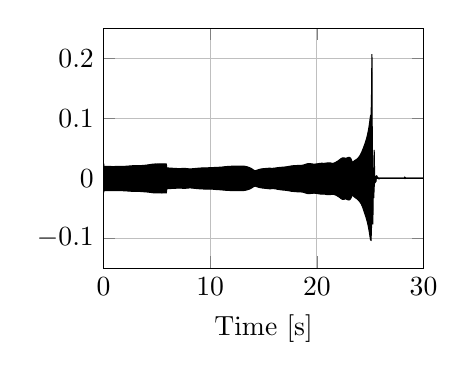
\begin{tikzpicture}

\begin{axis}[%
width=1.6in,
height=1.2in,
at={(0.758in,0.481in)},
scale only axis,
xmin=0,
xmax=30,
xmajorgrids,
ymin=-0.15,
ymax=0.25,
ymajorgrids,
xlabel={Time [s]},
axis background/.style={fill=white}
]
\addplot[fill=black,draw=black,forget plot] plot table[row sep=crcr]{%
2.08333333333333e-05	0.0252026319503784\\
0.0417454218822439	0.0196661949157715\\
0.0834700104311544	0.0195598602294922\\
0.125194598980065	0.0195558071136475\\
0.166919187528975	0.0195541381835938\\
0.208643776077886	0.0195835828781128\\
0.250368364626797	0.0195900201797485\\
0.292092953175707	0.0196053981781006\\
0.333817541724618	0.0195995569229126\\
0.375542130273528	0.0195615291595459\\
0.417266718822439	0.0195558071136475\\
0.458991307371349	0.0195248126983643\\
0.50071589592026	0.0195026397705078\\
0.54244048446917	0.0195032358169556\\
0.584165073018081	0.0194785594940186\\
0.625889661566991	0.0194668769836426\\
0.667614250115902	0.0194715261459351\\
0.709338838664812	0.019452691078186\\
0.751063427213723	0.0194509029388428\\
0.792788015762633	0.0194598436355591\\
0.834512604311544	0.019437313079834\\
0.876237192860454	0.019428014755249\\
0.917961781409365	0.0194230079650879\\
0.959686369958275	0.0194351673126221\\
1.00141095850719	0.0194576978683472\\
1.0431355470561	0.0194565057754517\\
1.08486013560501	0.0194827318191528\\
1.12658472415392	0.0194835662841797\\
1.16830931270283	0.0195174217224121\\
1.21003390125174	0.0195624828338623\\
1.25175848980065	0.0195828676223755\\
1.29348307834956	0.019595742225647\\
1.33520766689847	0.0196287631988525\\
1.37693225544738	0.0196471214294434\\
1.41865684399629	0.0196546316146851\\
1.4603814325452	0.0196762084960938\\
1.50210602109411	0.0196820497512817\\
1.54383060964302	0.0196628570556641\\
1.58555519819193	0.0196484327316284\\
1.62727978674084	0.0196454524993896\\
1.66900437528975	0.0196086168289185\\
1.71072896383866	0.0196232795715332\\
1.75245355238758	0.0196092128753662\\
1.79417814093649	0.0196236371994019\\
1.8359027294854	0.0196307897567749\\
1.87762731803431	0.0196537971496582\\
1.91935190658322	0.0196946859359741\\
1.96107649513213	0.0197988748550415\\
2.00280108368104	0.0197354555130005\\
2.04452567222995	0.0198073387145996\\
2.08625026077886	0.0198931694030762\\
2.12797484932777	0.0199716091156006\\
2.16969943787668	0.0200091600418091\\
2.21142402642559	0.020053505897522\\
2.2531486149745	0.0201040506362915\\
2.29487320352341	0.0201632976531982\\
2.33659779207232	0.0202457904815674\\
2.37832238062123	0.0202895402908325\\
2.42004696917014	0.0203609466552734\\
2.46177155771905	0.020421028137207\\
2.50349614626796	0.0204802751541138\\
2.54522073481687	0.0205562114715576\\
2.58694532336579	0.0205930471420288\\
2.6286699119147	0.0206351280212402\\
2.67039450046361	0.0206772089004517\\
2.71211908901252	0.0207411050796509\\
2.75384367756143	0.0207586288452148\\
2.79556826611034	0.0207893848419189\\
2.83729285465925	0.0208078622817993\\
2.87901744320816	0.0208115577697754\\
2.92074203175707	0.0208317041397095\\
2.96246662030598	0.0208277702331543\\
3.00419120885489	0.0208407640457153\\
3.0459157974038	0.0208303928375244\\
3.08764038595271	0.0208199024200439\\
3.12936497450162	0.0208157300949097\\
3.17108956305053	0.0208250284194946\\
3.21281415159944	0.0208191871643066\\
3.25453874014835	0.0208241939544678\\
3.29626332869726	0.0208383798599243\\
3.33798791724618	0.0208500623703003\\
3.37971250579509	0.0208836793899536\\
3.421437094344	0.0209195613861084\\
3.46316168289291	0.0209696292877197\\
3.50488627144182	0.0210163593292236\\
3.54661085999073	0.0210645198822021\\
3.58833544853964	0.0211191177368164\\
3.63006003708855	0.0211982727050781\\
3.67178462563746	0.0211962461471558\\
3.71350921418637	0.0212910175323486\\
3.75523380273528	0.0213606357574463\\
3.79695839128419	0.0214260816574097\\
3.8386829798331	0.0215083360671997\\
3.88040756838201	0.0215545892715454\\
3.92213215693092	0.0216106176376343\\
3.96385674547983	0.0217119455337524\\
4.00558133402874	0.0217915773391724\\
4.04730592257765	0.0218764543533325\\
4.08903051112656	0.0219782590866089\\
4.13075509967547	0.0221028327941895\\
4.17247968822439	0.0222001075744629\\
4.2142042767733	0.0223195552825928\\
4.25592886532221	0.0224275588989258\\
4.29765345387112	0.0225589275360107\\
4.33937804242003	0.0226887464523315\\
4.38110263096894	0.0227880477905273\\
4.42282721951785	0.0228797197341919\\
4.46455180806676	0.0230312347412109\\
4.50627639661567	0.0231308937072754\\
4.54800098516458	0.0232431888580322\\
4.58972557371349	0.0233291387557983\\
4.6314501622624	0.0234009027481079\\
4.67317475081131	0.0234928131103516\\
4.71489933936022	0.0235460996627808\\
4.75662392790913	0.0235745906829834\\
4.79834851645804	0.0236265659332275\\
4.84007310500695	0.0236315727233887\\
4.88179769355586	0.0236599445343018\\
4.92352228210478	0.0236629247665405\\
4.96524687065368	0.0236600637435913\\
5.0069714592026	0.0235556364059448\\
5.04869604775151	0.0237693786621094\\
5.09042063630042	0.0236787796020508\\
5.13214522484933	0.0237008333206177\\
5.17386981339824	0.023709774017334\\
5.21559440194715	0.0237230062484741\\
5.25731899049606	0.02374267578125\\
5.29904357904497	0.0237568616867065\\
5.34076816759388	0.0237780809402466\\
5.38249275614279	0.0238064527511597\\
5.4242173446917	0.0238009691238403\\
5.46594193324061	0.02381432056427\\
5.50766652178952	0.0238415002822876\\
5.54939111033843	0.0238394737243652\\
5.59111569888734	0.0238286256790161\\
5.63284028743625	0.0238009691238403\\
5.67456487598516	0.0237914323806763\\
5.71628946453407	0.0237894058227539\\
5.75801405308299	0.0237371921539307\\
5.7997386416319	0.023706316947937\\
5.84146323018081	0.0236771106719971\\
5.88318781872972	0.0236313343048096\\
5.92491240727863	0.0170843601226807\\
5.96663699582754	0.0169237852096558\\
6.00836158437645	0.017228364944458\\
6.05008617292536	0.0170774459838867\\
6.09181076147427	0.0169785022735596\\
6.13353535002318	0.0169421434402466\\
6.17525993857209	0.0169384479522705\\
6.216984527121	0.0168579816818237\\
6.25870911566991	0.0168157815933228\\
6.30043370421882	0.0167495012283325\\
6.34215829276773	0.016710638999939\\
6.38388288131664	0.016643762588501\\
6.42560746986555	0.0165911912918091\\
6.46733205841446	0.0165427923202515\\
6.50905664696338	0.0165140628814697\\
6.55078123551229	0.0164518356323242\\
6.5925058240612	0.0164361000061035\\
6.63423041261011	0.0163747072219849\\
6.67595500115902	0.0162972211837769\\
6.71767958970793	0.0162725448608398\\
6.75940417825684	0.0162316560745239\\
6.80112876680575	0.0161941051483154\\
6.84285335535466	0.0161614418029785\\
6.88457794390357	0.0160988569259644\\
6.92630253245248	0.0160497426986694\\
6.96802712100139	0.0160360336303711\\
7.0097517095503	0.0160067081451416\\
7.05147629809921	0.0159884691238403\\
7.09320088664812	0.015979528427124\\
7.13492547519703	0.0159775018692017\\
7.17665006374594	0.0159971714019775\\
7.21837465229485	0.0160175561904907\\
7.26009924084376	0.016065239906311\\
7.30182382939268	0.0161305665969849\\
7.34354841794159	0.0161781311035156\\
7.3852730064905	0.0162091255187988\\
7.42699759503941	0.0162465572357178\\
7.46872218358832	0.0162705183029175\\
7.51044677213723	0.0162796974182129\\
7.55217136068614	0.0162967443466187\\
7.59389594923505	0.0162732601165771\\
7.63562053778396	0.016247034072876\\
7.67734512633287	0.0162124633789063\\
7.71906971488178	0.0161486864089966\\
7.76079430343069	0.0160717964172363\\
7.8025188919796	0.0159912109375\\
7.84424348052851	0.0159145593643188\\
7.88596806907742	0.0158231258392334\\
7.92769265762633	0.0157468318939209\\
7.96941724617524	0.0156674385070801\\
8.01114183472416	0.0156195163726807\\
8.05286642327307	0.0155832767486572\\
8.09459101182198	0.0155816078186035\\
8.13631560037089	0.0155572891235352\\
8.1780401889198	0.0155682563781738\\
8.21976477746871	0.0155929327011108\\
8.26148936601762	0.0156328678131104\\
8.30321395456653	0.0157133340835571\\
8.34493854311544	0.0157613754272461\\
8.38666313166435	0.0158147811889648\\
8.42838772021326	0.0159033536911011\\
8.47011230876217	0.0159561634063721\\
8.51183689731108	0.0160245895385742\\
8.55356148585999	0.0160934925079346\\
8.5952860744089	0.0161852836608887\\
8.63701066295781	0.0162454843521118\\
8.67873525150672	0.0163184404373169\\
8.72045984005563	0.0163826942443848\\
8.76218442860454	0.0164344310760498\\
8.80390901715345	0.0164898633956909\\
8.84563360570237	0.0165649652481079\\
8.88735819425128	0.0166321992874146\\
8.92908278280018	0.0166976451873779\\
8.9708073713491	0.0167607069015503\\
9.01253195989801	0.0168074369430542\\
9.05425654844692	0.0168857574462891\\
9.09598113699583	0.0169258117675781\\
9.13770572554474	0.0169813632965088\\
9.17943031409365	0.0170243978500366\\
9.22115490264256	0.0170719623565674\\
9.26287949119147	0.0171010494232178\\
9.30460407974038	0.0171144008636475\\
9.34632866828929	0.0171386003494263\\
9.3880532568382	0.0171716213226318\\
9.42977784538711	0.0171942710876465\\
9.47150243393602	0.0172275304794312\\
9.51322702248493	0.0172395706176758\\
9.55495161103384	0.0172784328460693\\
9.59667619958275	0.017261266708374\\
9.63840078813166	0.0173088312149048\\
9.68012537668058	0.0173405408859253\\
9.72184996522949	0.0173261165618896\\
9.7635745537784	0.0173478126525879\\
9.80529914232731	0.017365574836731\\
9.84702373087622	0.0173982381820679\\
9.88874831942513	0.0174416303634644\\
9.93047290797404	0.0174491405487061\\
9.97219749652295	0.0174757242202759\\
10.0139220850719	0.017493724822998\\
10.0556466736208	0.0175291299819946\\
10.0973712621697	0.017573356628418\\
10.1390958507186	0.0176050662994385\\
10.1808204392675	0.0176557302474976\\
10.2225450278164	0.0176624059677124\\
10.2642696163653	0.0177156925201416\\
10.3059942049142	0.0177527666091919\\
10.3477187934631	0.0177849531173706\\
10.3894433820121	0.0178321599960327\\
10.431167970561	0.0178847312927246\\
10.4728925591099	0.0179171562194824\\
10.5146171476588	0.0179526805877686\\
10.5563417362077	0.0180047750473022\\
10.5980663247566	0.0180366039276123\\
10.6397909133055	0.0180578231811523\\
10.6815155018544	0.0181267261505127\\
10.7232400904033	0.0181165933609009\\
10.7649646789523	0.0181654691696167\\
10.8066892675012	0.0182121992111206\\
10.8484138560501	0.0182552337646484\\
10.890138444599	0.0182923078536987\\
10.9318630331479	0.0183515548706055\\
10.9735876216968	0.0184154510498047\\
11.0153122102457	0.0184671878814697\\
11.0570367987946	0.0185129642486572\\
11.0987613873435	0.0185738801956177\\
11.1404859758924	0.0186415910720825\\
11.1822105644414	0.0187274217605591\\
11.2239351529903	0.0188238620758057\\
11.2656597415392	0.0189311504364014\\
11.3073843300881	0.0189719200134277\\
11.349108918637	0.0190703868865967\\
11.3908335071859	0.019139289855957\\
11.4325580957348	0.0192180871963501\\
11.4742826842837	0.0192832946777344\\
11.5160072728326	0.0193512439727783\\
11.5577318613816	0.0194180011749268\\
11.5994564499305	0.0194872617721558\\
11.6411810384794	0.0195498466491699\\
11.6829056270283	0.0195857286453247\\
11.7246302155772	0.0196366310119629\\
11.7663548041261	0.0196753740310669\\
11.808079392675	0.0197402238845825\\
11.8498039812239	0.0197427272796631\\
11.8915285697728	0.0197911262512207\\
11.9332531583217	0.0198477506637573\\
11.9749777468707	0.0198787450790405\\
12.0167023354196	0.019885778427124\\
12.0584269239685	0.0199346542358398\\
12.1001515125174	0.0199596881866455\\
12.1418761010663	0.0199788808822632\\
12.1836006896152	0.0200355052947998\\
12.2253252781641	0.0200496912002563\\
12.267049866713	0.0200458765029907\\
12.3087744552619	0.0199846029281616\\
12.3504990438108	0.0200029611587524\\
12.3922236323598	0.0199966430664063\\
12.4339482209087	0.0199939012527466\\
12.4756728094576	0.0200033187866211\\
12.5173973980065	0.0200154781341553\\
12.5591219865554	0.0200347900390625\\
12.6008465751043	0.0200710296630859\\
12.6425711636532	0.0200951099395752\\
12.6842957522021	0.0201143026351929\\
12.726020340751	0.0201265811920166\\
12.7677449293	0.0201277732849121\\
12.8094695178489	0.0201374292373657\\
12.8511941063978	0.020142674446106\\
12.8929186949467	0.0201535224914551\\
12.9346432834956	0.0201476812362671\\
12.9763678720445	0.0201466083526611\\
13.0180924605934	0.020128607749939\\
13.0598170491423	0.0200852155685425\\
13.1015416376912	0.0200825929641724\\
13.1432662262401	0.0200129747390747\\
13.1849908147891	0.0199425220489502\\
13.226715403338	0.0198256969451904\\
13.2684399918869	0.0197237730026245\\
13.3101645804358	0.0195869207382202\\
13.3518891689847	0.0194164514541626\\
13.3936137575336	0.0192761421203613\\
13.4353383460825	0.0190843343734741\\
13.4770629346314	0.0188726186752319\\
13.5187875231803	0.018642783164978\\
13.5605121117293	0.0184153318405151\\
13.6022367002782	0.0181758403778076\\
13.6439612888271	0.017902135848999\\
13.685685877376	0.0176130533218384\\
13.7274104659249	0.0172675848007202\\
13.7691350544738	0.016897439956665\\
13.8108596430227	0.0165574550628662\\
13.8525842315716	0.0160777568817139\\
13.8943088201205	0.0156558752059937\\
13.9360334086694	0.0151234865188599\\
13.9777579972184	0.0146352052688599\\
14.0194825857673	0.0140862464904785\\
14.0612071743162	0.0136113166809082\\
14.1029317628651	0.0131813287734985\\
14.144656351414	0.0128709077835083\\
14.1863809399629	0.0126913785934448\\
14.2281055285118	0.0126174688339233\\
14.2698301170607	0.0126955509185791\\
14.3115547056096	0.0129036903381348\\
14.3532792941586	0.0131478309631348\\
14.3950038827075	0.0134261846542358\\
14.4367284712564	0.0136877298355103\\
14.4784530598053	0.0139557123184204\\
14.5201776483542	0.014224648475647\\
14.5619022369031	0.0144333839416504\\
14.603626825452	0.0146486759185791\\
14.6453514140009	0.0148535966873169\\
14.6870760025498	0.0150058269500732\\
14.7288005910988	0.0152024030685425\\
14.7705251796477	0.0153254270553589\\
14.8122497681966	0.0154402256011963\\
14.8539743567455	0.0155432224273682\\
14.8956989452944	0.0156687498092651\\
14.9374235338433	0.0157575607299805\\
14.9791481223922	0.0158365964889526\\
15.0208727109411	0.0159083604812622\\
15.06259729949	0.0159753561019897\\
15.1043218880389	0.0160367488861084\\
15.1460464765879	0.0160804986953735\\
15.1877710651368	0.0161639451980591\\
15.2294956536857	0.0162357091903687\\
15.2712202422346	0.0163024663925171\\
15.3129448307835	0.0163722038269043\\
15.3546694193324	0.0164440870285034\\
15.3963940078813	0.0164902210235596\\
15.4381185964302	0.0165249109268188\\
15.4798431849791	0.016572117805481\\
15.521567773528	0.0165891647338867\\
15.563292362077	0.016568660736084\\
15.6050169506259	0.0165624618530273\\
15.6467415391748	0.0165637731552124\\
15.6884661277237	0.0165224075317383\\
15.7301907162726	0.0165125131607056\\
15.7719153048215	0.0164953470230103\\
15.8136398933704	0.0165133476257324\\
15.8553644819193	0.0165115594863892\\
15.8970890704682	0.0165470838546753\\
15.9388136590172	0.0166467428207397\\
15.9805382475661	0.0166705846786499\\
16.022262836115	0.0167520046234131\\
16.0639874246639	0.0168416500091553\\
16.1057120132128	0.0169697999954224\\
16.1474366017617	0.0170661211013794\\
16.1891611903106	0.0172029733657837\\
16.2308857788595	0.0173318386077881\\
16.2726103674084	0.017427921295166\\
16.3143349559573	0.0175305604934692\\
16.3560595445063	0.017619252204895\\
16.3977841330552	0.0177319049835205\\
16.4395087216041	0.0178070068359375\\
16.481233310153	0.0179022550582886\\
16.5229578987019	0.017980694770813\\
16.5646824872508	0.0180490016937256\\
16.6064070757997	0.0180948972702026\\
16.6481316643486	0.0181583166122437\\
16.6898562528975	0.0182009935379028\\
16.7315808414465	0.0182572603225708\\
16.7733054299954	0.0182993412017822\\
16.8150300185443	0.0183553695678711\\
16.8567546070932	0.0184321403503418\\
16.8984791956421	0.0185000896453857\\
16.940203784191	0.0185577869415283\\
16.9819283727399	0.018602728843689\\
17.0236529612888	0.0187180042266846\\
17.0653775498377	0.0188030004501343\\
17.1071021383867	0.0189168453216553\\
17.1488267269356	0.0190103054046631\\
17.1905513154845	0.0191226005554199\\
17.2322759040334	0.0192161798477173\\
17.2740004925823	0.0193425416946411\\
17.3157250811312	0.019458532333374\\
17.3574496696801	0.0195962190628052\\
17.399174258229	0.0197238922119141\\
17.4408988467779	0.0198369026184082\\
17.4826234353268	0.019974946975708\\
17.5243480238758	0.0201324224472046\\
17.5660726124247	0.0202901363372803\\
17.6077972009736	0.0204662084579468\\
17.6495217895225	0.0205678939819336\\
17.6912463780714	0.0206447839736938\\
17.7329709666203	0.0206948518753052\\
17.7746955551692	0.0207159519195557\\
17.8164201437181	0.020727276802063\\
17.858144732267	0.0207618474960327\\
17.8998693208159	0.0207719802856445\\
17.9415939093649	0.02080237865448\\
17.9833184979138	0.020844578742981\\
18.0250430864627	0.0209076404571533\\
18.0667676750116	0.0209413766860962\\
18.1084922635605	0.0210739374160767\\
18.1502168521094	0.021175742149353\\
18.1919414406583	0.0212005376815796\\
18.2336660292072	0.0212287902832031\\
18.2753906177561	0.0212538242340088\\
18.3171152063051	0.0212697982788086\\
18.358839794854	0.0212750434875488\\
18.4005643834029	0.0212739706039429\\
18.4422889719518	0.0213068723678589\\
18.4840135605007	0.0213649272918701\\
18.5257381490496	0.0214124917984009\\
18.5674627375985	0.0214804410934448\\
18.6091873261474	0.021593451499939\\
18.6509119146963	0.0216748714447021\\
18.6926365032453	0.0217387676239014\\
18.7343610917942	0.0219330787658691\\
18.7760856803431	0.0221517086029053\\
18.817810268892	0.0224329233169556\\
18.8595348574409	0.0226765871047974\\
18.9012594459898	0.0229390859603882\\
18.9429840345387	0.0231872797012329\\
18.9847086230876	0.0233813524246216\\
19.0264332116365	0.0236054658889771\\
19.0681578001854	0.0238147974014282\\
19.1098823887344	0.0240134000778198\\
19.1516069772833	0.0241340398788452\\
19.1933315658322	0.0242315530776978\\
19.2350561543811	0.0242862701416016\\
19.27678074293	0.0243122577667236\\
19.3185053314789	0.0242971181869507\\
19.3602299200278	0.0242471694946289\\
19.4019545085767	0.0241547822952271\\
19.4436790971256	0.0240551233291626\\
19.4854036856745	0.0239152908325195\\
19.5271282742235	0.0238051414489746\\
19.5688528627724	0.0237158536911011\\
19.6105774513213	0.0236446857452393\\
19.6523020398702	0.0236036777496338\\
19.6940266284191	0.023579478263855\\
19.735751216968	0.0235514640808105\\
19.7774758055169	0.0235527753829956\\
19.8192003940658	0.0235652923583984\\
19.8609249826147	0.0236073732376099\\
19.9026495711637	0.0236579179763794\\
19.9443741597126	0.0237400531768799\\
19.9860987482615	0.0238206386566162\\
20.0278233368104	0.0239320993423462\\
20.0695479253593	0.0240556001663208\\
20.1112725139082	0.0241789817810059\\
20.1529971024571	0.0243054628372192\\
20.194721691006	0.0244289636611938\\
20.2364462795549	0.0245696306228638\\
20.2781708681038	0.0246896743774414\\
20.3198954566528	0.0247645378112793\\
20.3616200452017	0.0248233079910278\\
20.4033446337506	0.0248950719833374\\
20.4450692222995	0.0249079465866089\\
20.4867938108484	0.0249096155166626\\
20.5285183993973	0.0248874425888062\\
20.5702429879462	0.0248595476150513\\
20.6119675764951	0.0248348712921143\\
20.653692165044	0.0248099565505981\\
20.695416753593	0.0248129367828369\\
20.7371413421419	0.0248783826828003\\
20.7788659306908	0.0249456167221069\\
20.8205905192397	0.0250651836395264\\
20.8623151077886	0.0251662731170654\\
20.9040396963375	0.0252714157104492\\
20.9457642848864	0.0253703594207764\\
20.9874888734353	0.0254890918731689\\
21.0292134619842	0.0255718231201172\\
21.0709380505331	0.0256284475326538\\
21.1126626390821	0.0256397724151611\\
21.154387227631	0.0256414413452148\\
21.1961118161799	0.0255806446075439\\
21.2378364047288	0.0254940986633301\\
21.2795609932777	0.0253506898880005\\
21.3212855818266	0.0251891613006592\\
21.3630101703755	0.025056004524231\\
21.4047347589244	0.0249054431915283\\
21.4464593474733	0.0248575210571289\\
21.4881839360223	0.0247853994369507\\
21.5299085245712	0.0248724222183228\\
21.5716331131201	0.0250217914581299\\
21.613357701669	0.0252604484558105\\
21.6550822902179	0.0255463123321533\\
21.6968068787668	0.0258597135543823\\
21.7385314673157	0.0262342691421509\\
21.7802560558646	0.0266420841217041\\
21.8219806444135	0.0270575284957886\\
21.8637052329624	0.027531623840332\\
21.9054298215114	0.0279887914657593\\
21.9471544100603	0.0284712314605713\\
21.9888789986092	0.028952956199646\\
22.0306035871581	0.0294901132583618\\
22.072328175707	0.0300215482711792\\
22.1140527642559	0.0305451154708862\\
22.1557773528048	0.0311292409896851\\
22.1975019413537	0.0316804647445679\\
22.2392265299026	0.0322504043579102\\
22.2809511184516	0.0327503681182861\\
22.3226757070005	0.0332285165786743\\
22.3644002955494	0.0336005687713623\\
22.4061248840983	0.0338387489318848\\
22.4478494726472	0.03401780128479\\
22.4895740611961	0.0339645147323608\\
22.531298649745	0.0338977575302124\\
22.5730232382939	0.0337392091751099\\
22.6147478268428	0.0335226058959961\\
22.6564724153917	0.033193826675415\\
22.6981970039407	0.0330818891525269\\
22.7399215924896	0.0332854986190796\\
22.7816461810385	0.0334283113479614\\
22.8233707695874	0.0338183641433716\\
22.8650953581363	0.0340921878814697\\
22.9068199466852	0.0344362258911133\\
22.9485445352341	0.0348231792449951\\
22.990269123783	0.0348302125930786\\
23.0319937123319	0.0347589254379272\\
23.0737183008809	0.0344734191894531\\
23.1154428894298	0.033944845199585\\
23.1571674779787	0.0333338975906372\\
23.1988920665276	0.0321611166000366\\
23.2406166550765	0.0300352573394775\\
23.2823412436254	0.0282227993011475\\
23.3240658321743	0.0270638465881348\\
23.3657904207232	0.0267330408096313\\
23.4075150092721	0.0271947383880615\\
23.449239597821	0.0279620885848999\\
23.49096418637	0.0285921096801758\\
23.5326887749189	0.0292768478393555\\
23.5744133634678	0.0297896862030029\\
23.6161379520167	0.0302869081497192\\
23.6578625405656	0.030638575553894\\
23.6995871291145	0.0311297178268433\\
23.7413117176634	0.031591534614563\\
23.7830363062123	0.0320906639099121\\
23.8247608947612	0.0327820777893066\\
23.8664854833102	0.033638596534729\\
23.9082100718591	0.0345802307128906\\
23.949934660408	0.0355473756790161\\
23.9916592489569	0.0364874601364136\\
24.0333838375058	0.0375547409057617\\
24.0751084260547	0.0387784242630005\\
24.1168330146036	0.0402863025665283\\
24.1585576031525	0.0418564081192017\\
24.2002821917014	0.0434989929199219\\
24.2420067802503	0.0450118780136108\\
24.2837313687993	0.0468673706054688\\
24.3254559573482	0.0486793518066406\\
24.3671805458971	0.0506290197372437\\
24.408905134446	0.052638053894043\\
24.4506297229949	0.0547009706497192\\
24.4923543115438	0.0568504333496094\\
24.5340789000927	0.0589379072189331\\
24.5758034886416	0.0612823963165283\\
24.6175280771905	0.063717246055603\\
24.6592526657395	0.0663166046142578\\
24.7009772542884	0.069003701210022\\
24.7427018428373	0.072115421295166\\
24.7844264313862	0.0755225419998169\\
24.8261510199351	0.0793305635452271\\
24.867875608484	0.083472728729248\\
24.9096001970329	0.0883474349975586\\
24.9513247855818	0.0935847759246826\\
24.9930493741307	0.0997812747955322\\
25.0347739626796	0.104405403137207\\
25.0764985512286	0.104313254356384\\
25.1182231397775	0.128032088279724\\
25.1599477283264	0.206622838973999\\
25.2016723168753	0.00182950496673584\\
25.2433969054242	-0.00010228157043457\\
25.2851214939731	0.0175950527191162\\
25.326846082522	0.00960516929626465\\
25.3685706710709	0.0472007989883423\\
25.4102952596198	0.00513529777526855\\
25.4520198481687	-0.0037391185760498\\
25.4937444367177	-0.00510489940643311\\
25.5354690252666	0.00155222415924072\\
25.5771936138155	0.00397324562072754\\
25.6189182023644	0.00366842746734619\\
25.6606427909133	0.00189435482025146\\
25.7023673794622	0.00131595134735107\\
25.7440919680111	0.000153541564941406\\
25.78581655656	-0.00023353099822998\\
25.8275411451089	-0.00059044361114502\\
25.8692657336579	-0.000110149383544922\\
25.9109903222068	0.000211477279663086\\
25.9527149107557	0.000216484069824219\\
25.9944394993046	9.76324081420898e-05\\
26.0361640878535	0.000136375427246094\\
26.0778886764024	0.000159502029418945\\
26.1196132649513	8.30888748168945e-05\\
26.1613378535002	3.33786010742188e-05\\
26.2030624420491	0.000106334686279297\\
26.2447870305981	0.000101327896118164\\
26.286511619147	3.9219856262207e-05\\
26.3282362076959	9.47713851928711e-05\\
26.3699607962448	0.000104784965515137\\
26.4116853847937	7.89165496826172e-05\\
26.4534099733426	0.000110983848571777\\
26.4951345618915	0.000124454498291016\\
26.5368591504404	8.79764556884766e-05\\
26.5785837389893	0.000103473663330078\\
26.6203083275383	0.000116109848022461\\
26.6620329160872	9.84668731689453e-05\\
26.7037575046361	8.76188278198242e-05\\
26.745482093185	9.38177108764648e-05\\
26.7872066817339	8.44001770019531e-05\\
26.8289312702828	9.31024551391602e-05\\
26.8706558588317	9.21487808227539e-05\\
26.9123804473806	7.12871551513672e-05\\
26.9541050359295	4.97102737426758e-05\\
26.9958296244784	7.87973403930664e-05\\
27.0375542130274	7.68899917602539e-05\\
27.0792788015763	8.63075256347656e-05\\
27.1210033901252	7.96318054199219e-05\\
27.1627279786741	6.80685043334961e-05\\
27.204452567223	8.92877578735352e-05\\
27.2461771557719	7.21216201782227e-05\\
27.2879017443208	0.000113487243652344\\
27.3296263328697	7.46250152587891e-05\\
27.3713509214186	7.27176666259766e-05\\
27.4130755099675	5.68628311157227e-05\\
27.4548000985165	7.42673873901367e-05\\
27.4965246870654	5.09023666381836e-05\\
27.5382492756143	4.62532043457031e-05\\
27.5799738641632	0.00013434886932373\\
27.6216984527121	0.000106930732727051\\
27.663423041261	9.69171524047852e-05\\
27.7051476298099	0.000105619430541992\\
27.7468722183588	9.02414321899414e-05\\
27.7885968069077	8.44001770019531e-05\\
27.8303213954567	8.51154327392578e-05\\
27.8720459840056	0.000154376029968262\\
27.9137705725545	8.51154327392578e-05\\
27.9554951611034	0.000194549560546875\\
27.9972197496523	8.30888748168945e-05\\
28.0389443382012	7.60555267333984e-05\\
28.0806689267501	7.96318054199219e-05\\
28.122393515299	9.39369201660156e-05\\
28.1641181038479	0.000158905982971191\\
28.2058426923968	0.000211477279663086\\
28.2475672809458	0.00165641307830811\\
28.2892918694947	0.00073695182800293\\
28.3310164580436	9.63211059570313e-05\\
28.3727410465925	7.39097595214844e-05\\
28.4144656351414	7.80820846557617e-05\\
28.4561902236903	7.02142715454102e-05\\
28.4979148122392	3.85046005249023e-05\\
28.5396394007881	6.18696212768555e-05\\
28.581363989337	1.91926956176758e-05\\
28.623088577886	3.50475311279297e-05\\
28.6648131664349	5.10215759277344e-05\\
28.7065377549838	4.33921813964844e-05\\
28.7482623435327	5.88893890380859e-05\\
28.7899869320816	4.54187393188477e-05\\
28.8317115206305	4.17232513427734e-05\\
28.8734361091794	5.35249710083008e-05\\
28.9151606977283	4.35113906860352e-05\\
28.9568852862772	5.63859939575195e-05\\
28.9986098748261	5.51939010620117e-05\\
29.0403344633751	4.43458557128906e-05\\
29.082059051924	4.25577163696289e-05\\
29.1237836404729	6.04391098022461e-05\\
29.1655082290218	6.71148300170898e-05\\
29.2072328175707	7.17639923095703e-05\\
29.2489574061196	3.51667404174805e-05\\
29.2906819946685	3.68356704711914e-05\\
29.3324065832174	4.18424606323242e-05\\
29.3741311717663	5.17368316650391e-05\\
29.4158557603153	6.52074813842773e-05\\
29.4575803488642	5.97238540649414e-05\\
29.4993049374131	4.8518180847168e-05\\
29.541029525962	3.9219856262207e-05\\
29.5827541145109	4.01735305786133e-05\\
29.6244787030598	3.50475311279297e-05\\
29.6662032916087	5.87701797485352e-05\\
29.7079278801576	5.17368316650391e-05\\
29.7496524687065	4.62532043457031e-05\\
29.7913770572554	4.88758087158203e-05\\
29.8331016458044	3.21865081787109e-05\\
29.8748262343533	3.08752059936523e-05\\
29.9165508229022	4.37498092651367e-05\\
29.9582754114511	5.92470169067383e-05\\
30	4.67300415039063e-05\\
}
\closedcycle;
\addplot[fill=black,draw=black,forget plot] plot table[row sep=crcr]{%
2.08333333333333e-05	-0.023579478263855\\
0.0417454218822439	-0.0206550359725952\\
0.0834700104311544	-0.0206233263015747\\
0.125194598980065	-0.0206409692764282\\
0.166919187528975	-0.0206311941146851\\
0.208643776077886	-0.0205899477005005\\
0.250368364626797	-0.0205674171447754\\
0.292092953175707	-0.0205302238464355\\
0.333817541724618	-0.0205274820327759\\
0.375542130273528	-0.0205377340316772\\
0.417266718822439	-0.020534873008728\\
0.458991307371349	-0.0205378532409668\\
0.50071589592026	-0.0205215215682983\\
0.54244048446917	-0.0205061435699463\\
0.584165073018081	-0.0205219984054565\\
0.625889661566991	-0.0204943418502808\\
0.667614250115902	-0.0204542875289917\\
0.709338838664812	-0.0204310417175293\\
0.751063427213723	-0.0204265117645264\\
0.792788015762633	-0.0204039812088013\\
0.834512604311544	-0.0204031467437744\\
0.876237192860454	-0.0203876495361328\\
0.917961781409365	-0.0203948020935059\\
0.959686369958275	-0.0203834772109985\\
1.00141095850719	-0.0203601121902466\\
1.0431355470561	-0.0203800201416016\\
1.08486013560501	-0.0203700065612793\\
1.12658472415392	-0.0204088687896729\\
1.16830931270283	-0.0204001665115356\\
1.21003390125174	-0.0204088687896729\\
1.25175848980065	-0.0204339027404785\\
1.29348307834956	-0.0204442739486694\\
1.33520766689847	-0.0204689502716064\\
1.37693225544738	-0.0205010175704956\\
1.41865684399629	-0.0204367637634277\\
1.4603814325452	-0.0205528736114502\\
1.50210602109411	-0.0205986499786377\\
1.54383060964302	-0.0206171274185181\\
1.58555519819193	-0.0206534862518311\\
1.62727978674084	-0.020700216293335\\
1.66900437528975	-0.0207151174545288\\
1.71072896383866	-0.0207169055938721\\
1.75245355238758	-0.0207256078720093\\
1.79417814093649	-0.0207580327987671\\
1.8359027294854	-0.0207885503768921\\
1.87762731803431	-0.020816445350647\\
1.91935190658322	-0.0208886861801147\\
1.96107649513213	-0.0208624601364136\\
2.00280108368104	-0.0209550857543945\\
2.04452567222995	-0.0209997892379761\\
2.08625026077886	-0.0210025310516357\\
2.12797484932777	-0.0210417509078979\\
2.16969943787668	-0.0210747718811035\\
2.21142402642559	-0.0211694240570068\\
2.2531486149745	-0.0212162733078003\\
2.29487320352341	-0.0212785005569458\\
2.33659779207232	-0.0213222503662109\\
2.37832238062123	-0.0213861465454102\\
2.42004696917014	-0.0214494466781616\\
2.46177155771905	-0.0215213298797607\\
2.50349614626796	-0.0215605497360229\\
2.54522073481687	-0.0215951204299927\\
2.58694532336579	-0.0216288566589355\\
2.6286699119147	-0.0216867923736572\\
2.67039450046361	-0.02173912525177\\
2.71211908901252	-0.0217874050140381\\
2.75384367756143	-0.0217965841293335\\
2.79556826611034	-0.0218116044998169\\
2.83729285465925	-0.0218478441238403\\
2.87901744320816	-0.0218620300292969\\
2.92074203175707	-0.0218536853790283\\
2.96246662030598	-0.021858811378479\\
3.00419120885489	-0.02183997631073\\
3.0459157974038	-0.0218436717987061\\
3.08764038595271	-0.02186119556427\\
3.12936497450162	-0.0218538045883179\\
3.17108956305053	-0.0218511819839478\\
3.21281415159944	-0.0218641757965088\\
3.25453874014835	-0.0218712091445923\\
3.29626332869726	-0.0218818187713623\\
3.33798791724618	-0.0219129323959351\\
3.37971250579509	-0.0219534635543823\\
3.421437094344	-0.0219793319702148\\
3.46316168289291	-0.0220361948013306\\
3.50488627144182	-0.02208411693573\\
3.54661085999073	-0.0221425294876099\\
3.58833544853964	-0.022210955619812\\
3.63006003708855	-0.0222430229187012\\
3.67178462563746	-0.0223485231399536\\
3.71350921418637	-0.0223995447158813\\
3.75523380273528	-0.0224494934082031\\
3.79695839128419	-0.0225085020065308\\
3.8386829798331	-0.0225539207458496\\
3.88040756838201	-0.0225838422775269\\
3.92213215693092	-0.0226439237594604\\
3.96385674547983	-0.0227533578872681\\
4.00558133402874	-0.0227950811386108\\
4.04730592257765	-0.0228416919708252\\
4.08903051112656	-0.0229117870330811\\
4.13075509967547	-0.0229719877243042\\
4.17247968822439	-0.0230708122253418\\
4.2142042767733	-0.0231355428695679\\
4.25592886532221	-0.0232703685760498\\
4.29765345387112	-0.0233174562454224\\
4.33937804242003	-0.0234375\\
4.38110263096894	-0.0235351324081421\\
4.42282721951785	-0.023618221282959\\
4.46455180806676	-0.0237029790878296\\
4.50627639661567	-0.023835301399231\\
4.54800098516458	-0.0239487886428833\\
4.58972557371349	-0.0240225791931152\\
4.6314501622624	-0.0241239070892334\\
4.67317475081131	-0.0241935253143311\\
4.71489933936022	-0.024228572845459\\
4.75662392790913	-0.0242753028869629\\
4.79834851645804	-0.0243275165557861\\
4.84007310500695	-0.0243371725082397\\
4.88179769355586	-0.0243518352508545\\
4.92352228210478	-0.0243576765060425\\
4.96524687065368	-0.024360179901123\\
5.0069714592026	-0.0243475437164307\\
5.04869604775151	-0.024484395980835\\
5.09042063630042	-0.0243972539901733\\
5.13214522484933	-0.024404764175415\\
5.17386981339824	-0.0244338512420654\\
5.21559440194715	-0.0244594812393188\\
5.25731899049606	-0.0244648456573486\\
5.29904357904497	-0.0244845151901245\\
5.34076816759388	-0.0244945287704468\\
5.38249275614279	-0.0245064496994019\\
5.4242173446917	-0.0245194435119629\\
5.46594193324061	-0.0245504379272461\\
5.50766652178952	-0.0245078802108765\\
5.54939111033843	-0.0245212316513062\\
5.59111569888734	-0.0245189666748047\\
5.63284028743625	-0.0245095491409302\\
5.67456487598516	-0.0244981050491333\\
5.71628946453407	-0.0244677066802979\\
5.75801405308299	-0.0244376659393311\\
5.7997386416319	-0.0244119167327881\\
5.84146323018081	-0.0243830680847168\\
5.88318781872972	-0.0243401527404785\\
5.92491240727863	-0.0173517465591431\\
5.96663699582754	-0.0172023773193359\\
6.00836158437645	-0.0174857378005981\\
6.05008617292536	-0.0174034833908081\\
6.09181076147427	-0.0172989368438721\\
6.13353535002318	-0.0172704458236694\\
6.17525993857209	-0.0172390937805176\\
6.216984527121	-0.0172088146209717\\
6.25870911566991	-0.0171716213226318\\
6.30043370421882	-0.0171136856079102\\
6.34215829276773	-0.0170572996139526\\
6.38388288131664	-0.0170092582702637\\
6.42560746986555	-0.0169717073440552\\
6.46733205841446	-0.0169262886047363\\
6.50905664696338	-0.0168750286102295\\
6.55078123551229	-0.0168637037277222\\
6.5925058240612	-0.0167915821075439\\
6.63423041261011	-0.0167664289474487\\
6.67595500115902	-0.0167648792266846\\
6.71767958970793	-0.0167108774185181\\
6.75940417825684	-0.0166767835617065\\
6.80112876680575	-0.0166200399398804\\
6.84285335535466	-0.0165899991989136\\
6.88457794390357	-0.0165786743164063\\
6.92630253245248	-0.0165473222732544\\
6.96802712100139	-0.0165069103240967\\
7.0097517095503	-0.0164788961410522\\
7.05147629809921	-0.0164910554885864\\
7.09320088664812	-0.0165011882781982\\
7.13492547519703	-0.0164777040481567\\
7.17665006374594	-0.0164895057678223\\
7.21837465229485	-0.0165047645568848\\
7.26009924084376	-0.0165224075317383\\
7.30182382939268	-0.0165432691574097\\
7.34354841794159	-0.0165948867797852\\
7.3852730064905	-0.016639232635498\\
7.42699759503941	-0.0166875123977661\\
7.46872218358832	-0.0167175531387329\\
7.51044677213723	-0.0167485475540161\\
7.55217136068614	-0.0167577266693115\\
7.59389594923505	-0.0167492628097534\\
7.63562053778396	-0.0167118310928345\\
7.67734512633287	-0.016689658164978\\
7.71906971488178	-0.0166492462158203\\
7.76079430343069	-0.0165841579437256\\
7.8025188919796	-0.0165199041366577\\
7.84424348052851	-0.0164152383804321\\
7.88596806907742	-0.016349196434021\\
7.92769265762633	-0.0163037776947021\\
7.96941724617524	-0.016208291053772\\
8.01114183472416	-0.0161799192428589\\
8.05286642327307	-0.0161402225494385\\
8.09459101182198	-0.0161368846893311\\
8.13631560037089	-0.0161551237106323\\
8.1780401889198	-0.0161631107330322\\
8.21976477746871	-0.0162090063095093\\
8.26148936601762	-0.0162490606307983\\
8.30321395456653	-0.0163116455078125\\
8.34493854311544	-0.0164139270782471\\
8.38666313166435	-0.0164964199066162\\
8.42838772021326	-0.0165704488754272\\
8.47011230876217	-0.0166466236114502\\
8.51183689731108	-0.0167334079742432\\
8.55356148585999	-0.0168044567108154\\
8.5952860744089	-0.0168653726577759\\
8.63701066295781	-0.0169525146484375\\
8.67873525150672	-0.0170137882232666\\
8.72045984005563	-0.0170843601226807\\
8.76218442860454	-0.0171598196029663\\
8.80390901715345	-0.0172305107116699\\
8.84563360570237	-0.0172979831695557\\
8.88735819425128	-0.0173814296722412\\
8.92908278280018	-0.0174278020858765\\
8.9708073713491	-0.0174862146377563\\
9.01253195989801	-0.0175342559814453\\
9.05425654844692	-0.0175997018814087\\
9.09598113699583	-0.0176476240158081\\
9.13770572554474	-0.017676830291748\\
9.17943031409365	-0.0177227258682251\\
9.22115490264256	-0.0177469253540039\\
9.26287949119147	-0.0177766084671021\\
9.30460407974038	-0.0178029537200928\\
9.34632866828929	-0.0178709030151367\\
9.3880532568382	-0.0179080963134766\\
9.42977784538711	-0.017917275428772\\
9.47150243393602	-0.0179593563079834\\
9.51322702248493	-0.0179598331451416\\
9.55495161103384	-0.0179756879806519\\
9.59667619958275	-0.0179805755615234\\
9.63840078813166	-0.0179872512817383\\
9.68012537668058	-0.0179914236068726\\
9.72184996522949	-0.0180085897445679\\
9.7635745537784	-0.0180236101150513\\
9.80529914232731	-0.0180302858352661\\
9.84702373087622	-0.0180561542510986\\
9.88874831942513	-0.0180631875991821\\
9.93047290797404	-0.0180803537368774\\
9.97219749652295	-0.0180908441543579\\
10.0139220850719	-0.0180753469467163\\
10.0556466736208	-0.0181277990341187\\
10.0973712621697	-0.0181586742401123\\
10.1390958507186	-0.0181567668914795\\
10.1808204392675	-0.0181816816329956\\
10.2225450278164	-0.0182309150695801\\
10.2642696163653	-0.0182760953903198\\
10.3059942049142	-0.0183569192886353\\
10.3477187934631	-0.0184228420257568\\
10.3894433820121	-0.0184857845306396\\
10.431167970561	-0.018579363822937\\
10.4728925591099	-0.0186182260513306\\
10.5146171476588	-0.0186953544616699\\
10.5563417362077	-0.0187586545944214\\
10.5980663247566	-0.018807053565979\\
10.6397909133055	-0.0188767910003662\\
10.6815155018544	-0.0189163684844971\\
10.7232400904033	-0.0189580917358398\\
10.7649646789523	-0.0190116167068481\\
10.8066892675012	-0.0190404653549194\\
10.8484138560501	-0.0190988779067993\\
10.890138444599	-0.0191137790679932\\
10.9318630331479	-0.0191454887390137\\
10.9735876216968	-0.019208550453186\\
11.0153122102457	-0.0193091630935669\\
11.0570367987946	-0.0193337202072144\\
11.0987613873435	-0.0194271802902222\\
11.1404859758924	-0.0194764137268066\\
11.1822105644414	-0.019565224647522\\
11.2239351529903	-0.0196261405944824\\
11.2656597415392	-0.0196640491485596\\
11.3073843300881	-0.0197666883468628\\
11.349108918637	-0.0198172330856323\\
11.3908335071859	-0.0198853015899658\\
11.4325580957348	-0.0199508666992188\\
11.4742826842837	-0.0200226306915283\\
11.5160072728326	-0.0200650691986084\\
11.5577318613816	-0.0201363563537598\\
11.5994564499305	-0.0201640129089355\\
11.6411810384794	-0.0202010869979858\\
11.6829056270283	-0.0202364921569824\\
11.7246302155772	-0.0202765464782715\\
11.7663548041261	-0.0203347206115723\\
11.808079392675	-0.0203458070755005\\
11.8498039812239	-0.0203793048858643\\
11.8915285697728	-0.0203948020935059\\
11.9332531583217	-0.0204305648803711\\
11.9749777468707	-0.0204480886459351\\
12.0167023354196	-0.0204609632492065\\
12.0584269239685	-0.0204932689666748\\
12.1001515125174	-0.0204956531524658\\
12.1418761010663	-0.0205093622207642\\
12.1836006896152	-0.0205575227737427\\
12.2253252781641	-0.0206044912338257\\
12.267049866713	-0.0205936431884766\\
12.3087744552619	-0.0205252170562744\\
12.3504990438108	-0.020550012588501\\
12.3922236323598	-0.0204935073852539\\
12.4339482209087	-0.0205461978912354\\
12.4756728094576	-0.0205370187759399\\
12.5173973980065	-0.0205717086791992\\
12.5591219865554	-0.0205909013748169\\
12.6008465751043	-0.0205991268157959\\
12.6425711636532	-0.0206245183944702\\
12.6842957522021	-0.020621657371521\\
12.726020340751	-0.0206149816513062\\
12.7677449293	-0.0206171274185181\\
12.8094695178489	-0.0206117630004883\\
12.8511941063978	-0.0206212997436523\\
12.8929186949467	-0.0205870866775513\\
12.9346432834956	-0.0206025838851929\\
12.9763678720445	-0.0205825567245483\\
13.0180924605934	-0.0205703973770142\\
13.0598170491423	-0.0205336809158325\\
13.1015416376912	-0.0204759836196899\\
13.1432662262401	-0.0204193592071533\\
13.1849908147891	-0.020321249961853\\
13.226715403338	-0.0202198028564453\\
13.2684399918869	-0.0200797319412231\\
13.3101645804358	-0.0199527740478516\\
13.3518891689847	-0.0197756290435791\\
13.3936137575336	-0.0196079015731812\\
13.4353383460825	-0.0193984508514404\\
13.4770629346314	-0.0191981792449951\\
13.5187875231803	-0.0189844369888306\\
13.5605121117293	-0.0187491178512573\\
13.6022367002782	-0.0184566974639893\\
13.6439612888271	-0.018220067024231\\
13.685685877376	-0.0179322957992554\\
13.7274104659249	-0.0175908803939819\\
13.7691350544738	-0.0172412395477295\\
13.8108596430227	-0.0168406963348389\\
13.8525842315716	-0.0164436101913452\\
13.8943088201205	-0.0159670114517212\\
13.9360334086694	-0.0155180692672729\\
13.9777579972184	-0.0150215625762939\\
14.0194825857673	-0.0145455598831177\\
14.0612071743162	-0.0140774250030518\\
14.1029317628651	-0.0137002468109131\\
14.144656351414	-0.0133980512619019\\
14.1863809399629	-0.013235330581665\\
14.2281055285118	-0.0132846832275391\\
14.2698301170607	-0.0134497880935669\\
14.3115547056096	-0.0136580467224121\\
14.3532792941586	-0.0139237642288208\\
14.3950038827075	-0.0142141580581665\\
14.4367284712564	-0.0144933462142944\\
14.4784530598053	-0.0147548913955688\\
14.5201776483542	-0.0149476528167725\\
14.5619022369031	-0.0151650905609131\\
14.603626825452	-0.0153415203094482\\
14.6453514140009	-0.0155267715454102\\
14.6870760025498	-0.0156419277191162\\
14.7288005910988	-0.0157980918884277\\
14.7705251796477	-0.01591956615448\\
14.8122497681966	-0.0160800218582153\\
14.8539743567455	-0.0161597728729248\\
14.8956989452944	-0.0162812471389771\\
14.9374235338433	-0.0163697004318237\\
14.9791481223922	-0.0164555311203003\\
15.0208727109411	-0.0165287256240845\\
15.06259729949	-0.0165941715240479\\
15.1043218880389	-0.0166939496994019\\
15.1460464765879	-0.0167543888092041\\
15.1877710651368	-0.016822338104248\\
15.2294956536857	-0.0169036388397217\\
15.2712202422346	-0.0169987678527832\\
15.3129448307835	-0.0171036720275879\\
15.3546694193324	-0.01722252368927\\
15.3963940078813	-0.0173054933547974\\
15.4381185964302	-0.017369270324707\\
15.4798431849791	-0.0174156427383423\\
15.521567773528	-0.0174611806869507\\
15.563292362077	-0.0174987316131592\\
15.6050169506259	-0.0174720287322998\\
15.6467415391748	-0.0174695253372192\\
15.6884661277237	-0.0174558162689209\\
15.7301907162726	-0.0174344778060913\\
15.7719153048215	-0.0174111127853394\\
15.8136398933704	-0.0173563957214355\\
15.8553644819193	-0.0173189640045166\\
15.8970890704682	-0.0173122882843018\\
15.9388136590172	-0.0173076391220093\\
15.9805382475661	-0.0173790454864502\\
16.022262836115	-0.0174552202224731\\
16.0639874246639	-0.0175075531005859\\
16.1057120132128	-0.017642617225647\\
16.1474366017617	-0.0177702903747559\\
16.1891611903106	-0.0179281234741211\\
16.2308857788595	-0.0181002616882324\\
16.2726103674084	-0.0182489156723022\\
16.3143349559573	-0.0183770656585693\\
16.3560595445063	-0.0184937715530396\\
16.3977841330552	-0.0186386108398438\\
16.4395087216041	-0.0187474489212036\\
16.481233310153	-0.0188472270965576\\
16.5229578987019	-0.0189435482025146\\
16.5646824872508	-0.0190732479095459\\
16.6064070757997	-0.0191655158996582\\
16.6481316643486	-0.0192544460296631\\
16.6898562528975	-0.0193567276000977\\
16.7315808414465	-0.0194664001464844\\
16.7733054299954	-0.0195397138595581\\
16.8150300185443	-0.0196398496627808\\
16.8567546070932	-0.0196866989135742\\
16.8984791956421	-0.0197526216506958\\
16.940203784191	-0.0197983980178833\\
16.9819283727399	-0.0198843479156494\\
17.0236529612888	-0.019961953163147\\
17.0653775498377	-0.0200380086898804\\
17.1071021383867	-0.0201402902603149\\
17.1488267269356	-0.0202381610870361\\
17.1905513154845	-0.0203509330749512\\
17.2322759040334	-0.0204297304153442\\
17.2740004925823	-0.0205373764038086\\
17.3157250811312	-0.0206570625305176\\
17.3574496696801	-0.0208085775375366\\
17.399174258229	-0.0209213495254517\\
17.4408988467779	-0.021075963973999\\
17.4826234353268	-0.0212304592132568\\
17.5243480238758	-0.0213847160339355\\
17.5660726124247	-0.0215600728988647\\
17.6077972009736	-0.021699070930481\\
17.6495217895225	-0.0218133926391602\\
17.6912463780714	-0.0219072103500366\\
17.7329709666203	-0.0219838619232178\\
17.7746955551692	-0.022010326385498\\
17.8164201437181	-0.0220339298248291\\
17.858144732267	-0.0220590829849243\\
17.8998693208159	-0.0220861434936523\\
17.9415939093649	-0.0221391916275024\\
17.9833184979138	-0.0222084522247314\\
18.0250430864627	-0.0222910642623901\\
18.0667676750116	-0.0223599672317505\\
18.1084922635605	-0.0224792957305908\\
18.1502168521094	-0.0225588083267212\\
18.1919414406583	-0.0225856304168701\\
18.2336660292072	-0.0226218700408936\\
18.2753906177561	-0.0226372480392456\\
18.3171152063051	-0.0226311683654785\\
18.358839794854	-0.0226569175720215\\
18.4005643834029	-0.0226624011993408\\
18.4422889719518	-0.0226974487304688\\
18.4840135605007	-0.0227479934692383\\
18.5257381490496	-0.0227841138839722\\
18.5674627375985	-0.0228906869888306\\
18.6091873261474	-0.0229544639587402\\
18.6509119146963	-0.0230441093444824\\
18.6926365032453	-0.0231479406356812\\
18.7343610917942	-0.0233550071716309\\
18.7760856803431	-0.0236010551452637\\
18.817810268892	-0.0238543748855591\\
18.8595348574409	-0.0241819620132446\\
18.9012594459898	-0.0244064331054688\\
18.9429840345387	-0.0246450901031494\\
18.9847086230876	-0.0248016119003296\\
19.0264332116365	-0.0249960422515869\\
19.0681578001854	-0.0252091884613037\\
19.1098823887344	-0.0253455638885498\\
19.1516069772833	-0.0254670381546021\\
19.1933315658322	-0.0255337953567505\\
19.2350561543811	-0.0255684852600098\\
19.27678074293	-0.0255750417709351\\
19.3185053314789	-0.02555251121521\\
19.3602299200278	-0.025492787361145\\
19.4019545085767	-0.0253742933273315\\
19.4436790971256	-0.0252934694290161\\
19.4854036856745	-0.0251970291137695\\
19.5271282742235	-0.0251103639602661\\
19.5688528627724	-0.0250321626663208\\
19.6105774513213	-0.0249638557434082\\
19.6523020398702	-0.0249471664428711\\
19.6940266284191	-0.0249420404434204\\
19.735751216968	-0.0249300003051758\\
19.7774758055169	-0.0249425172805786\\
19.8192003940658	-0.0249909162521362\\
19.8609249826147	-0.0250338315963745\\
19.9026495711637	-0.0250961780548096\\
19.9443741597126	-0.0251920223236084\\
19.9860987482615	-0.025265097618103\\
20.0278233368104	-0.0253690481185913\\
20.0695479253593	-0.0255012512207031\\
20.1112725139082	-0.0256388187408447\\
20.1529971024571	-0.0257998704910278\\
20.194721691006	-0.0259189605712891\\
20.2364462795549	-0.0260286331176758\\
20.2781708681038	-0.0261536836624146\\
20.3198954566528	-0.0262869596481323\\
20.3616200452017	-0.0263389348983765\\
20.4033446337506	-0.0263962745666504\\
20.4450692222995	-0.0264378786087036\\
20.4867938108484	-0.0264571905136108\\
20.5285183993973	-0.0264530181884766\\
20.5702429879462	-0.0264363288879395\\
20.6119675764951	-0.0264163017272949\\
20.653692165044	-0.0264278650283813\\
20.695416753593	-0.0264804363250732\\
20.7371413421419	-0.0265471935272217\\
20.7788659306908	-0.0266481637954712\\
20.8205905192397	-0.0267904996871948\\
20.8623151077886	-0.0269136428833008\\
20.9040396963375	-0.0270541906356812\\
20.9457642848864	-0.0271708965301514\\
20.9874888734353	-0.0272594690322876\\
21.0292134619842	-0.0273599624633789\\
21.0709380505331	-0.02739417552948\\
21.1126626390821	-0.0274195671081543\\
21.154387227631	-0.0273842811584473\\
21.1961118161799	-0.0273327827453613\\
21.2378364047288	-0.0272507667541504\\
21.2795609932777	-0.0270979404449463\\
21.3212855818266	-0.0269280672073364\\
21.3630101703755	-0.0268005132675171\\
21.4047347589244	-0.0266823768615723\\
21.4464593474733	-0.0266032218933105\\
21.4881839360223	-0.0266386270523071\\
21.5299085245712	-0.0267366170883179\\
21.5716331131201	-0.0268681049346924\\
21.613357701669	-0.0270432233810425\\
21.6550822902179	-0.0272970199584961\\
21.6968068787668	-0.0275582075119019\\
21.7385314673157	-0.027861475944519\\
21.7802560558646	-0.0281882286071777\\
21.8219806444135	-0.0285769701004028\\
21.8637052329624	-0.0289305448532104\\
21.9054298215114	-0.0294040441513062\\
21.9471544100603	-0.0297894477844238\\
21.9888789986092	-0.0302231311798096\\
22.0306035871581	-0.0306861400604248\\
22.072328175707	-0.0311977863311768\\
22.1140527642559	-0.0317342281341553\\
22.1557773528048	-0.0322719812393188\\
22.1975019413537	-0.0328465700149536\\
22.2392265299026	-0.0334961414337158\\
22.2809511184516	-0.0339769124984741\\
22.3226757070005	-0.0344617366790771\\
22.3644002955494	-0.0348492860794067\\
22.4061248840983	-0.0350879430770874\\
22.4478494726472	-0.0352791547775269\\
22.4895740611961	-0.0352586507797241\\
22.531298649745	-0.0351810455322266\\
22.5730232382939	-0.034961462020874\\
22.6147478268428	-0.0346866846084595\\
22.6564724153917	-0.034406304359436\\
22.6981970039407	-0.0343616008758545\\
22.7399215924896	-0.034645676612854\\
22.7816461810385	-0.0349293947219849\\
22.8233707695874	-0.0352602005004883\\
22.8650953581363	-0.0355678796768188\\
22.9068199466852	-0.0358340740203857\\
22.9485445352341	-0.0361557006835938\\
22.990269123783	-0.0361953973770142\\
23.0319937123319	-0.0361014604568481\\
23.0737183008809	-0.035765528678894\\
23.1154428894298	-0.0350303649902344\\
23.1571674779787	-0.03395676612854\\
23.1988920665276	-0.0328094959259033\\
23.2406166550765	-0.0308859348297119\\
23.2823412436254	-0.0295355319976807\\
23.3240658321743	-0.0284759998321533\\
23.3657904207232	-0.0285098552703857\\
23.4075150092721	-0.0291345119476318\\
23.449239597821	-0.0299686193466187\\
23.49096418637	-0.0307345390319824\\
23.5326887749189	-0.0314371585845947\\
23.5744133634678	-0.0320383310317993\\
23.6161379520167	-0.0326122045516968\\
23.6578625405656	-0.0330005884170532\\
23.6995871291145	-0.0335551500320435\\
23.7413117176634	-0.034123420715332\\
23.7830363062123	-0.0347558259963989\\
23.8247608947612	-0.0353759527206421\\
23.8664854833102	-0.0360560417175293\\
23.9082100718591	-0.0367611646652222\\
23.949934660408	-0.037691593170166\\
23.9916592489569	-0.0384962558746338\\
24.0333838375058	-0.0394431352615356\\
24.0751084260547	-0.040552020072937\\
24.1168330146036	-0.0417412519454956\\
24.1585576031525	-0.0429370403289795\\
24.2002821917014	-0.0444494485855103\\
24.2420067802503	-0.0461583137512207\\
24.2837313687993	-0.0480393171310425\\
24.3254559573482	-0.050065279006958\\
24.3671805458971	-0.052216649055481\\
24.408905134446	-0.0543694496154785\\
24.4506297229949	-0.0565832853317261\\
24.4923543115438	-0.0587095022201538\\
24.5340789000927	-0.0610123872756958\\
24.5758034886416	-0.0632199048995972\\
24.6175280771905	-0.0657780170440674\\
24.6592526657395	-0.0682888031005859\\
24.7009772542884	-0.0710229873657227\\
24.7427018428373	-0.0740045309066772\\
24.7844264313862	-0.0772976875305176\\
24.8261510199351	-0.0806517601013184\\
24.867875608484	-0.084714412689209\\
24.9096001970329	-0.0890249013900757\\
24.9513247855818	-0.0938159227371216\\
24.9930493741307	-0.0988327264785767\\
25.0347739626796	-0.102910280227661\\
25.0764985512286	-0.103281259536743\\
25.1182231397775	-0.0803931951522827\\
25.1599477283264	-0.0682003498077393\\
25.2016723168753	-0.00261509418487549\\
25.2433969054242	-0.0768238306045532\\
25.2851214939731	-0.0187219381332397\\
25.326846082522	-0.0330673456192017\\
25.3685706710709	-0.0145893096923828\\
25.4102952596198	-0.00689935684204102\\
25.4520198481687	-0.0058441162109375\\
25.4937444367177	-0.00629651546478271\\
25.5354690252666	-0.00512027740478516\\
25.5771936138155	0.00152826309204102\\
25.6189182023644	0.00184798240661621\\
25.6606427909133	0.00129961967468262\\
25.7023673794622	8.392333984375e-05\\
25.7440919680111	-0.00028538703918457\\
25.78581655656	-0.00076758861541748\\
25.8275411451089	-0.000874042510986328\\
25.8692657336579	-0.000668764114379883\\
25.9109903222068	-0.000225663185119629\\
25.9527149107557	-1.2516975402832e-05\\
25.9944394993046	-0.000110030174255371\\
26.0361640878535	-7.46250152587891e-05\\
26.0778886764024	-2.33650207519531e-05\\
26.1196132649513	-0.000139236450195313\\
26.1613378535002	-0.000165104866027832\\
26.2030624420491	-6.55651092529297e-05\\
26.2447870305981	-9.17911529541016e-05\\
26.286511619147	-0.000103950500488281\\
26.3282362076959	-8.74996185302734e-05\\
26.3699607962448	-8.79764556884766e-05\\
26.4116853847937	-0.000130891799926758\\
26.4534099733426	-0.000128388404846191\\
26.4951345618915	-0.000122666358947754\\
26.5368591504404	-0.000141739845275879\\
26.5785837389893	-0.000144720077514648\\
26.6203083275383	-0.000100612640380859\\
26.6620329160872	-9.76324081420898e-05\\
26.7037575046361	-0.000108957290649414\\
26.745482093185	-0.000105023384094238\\
26.7872066817339	-0.000105857849121094\\
26.8289312702828	-9.50098037719727e-05\\
26.8706558588317	-5.80549240112305e-05\\
26.9123804473806	-6.49690628051758e-05\\
26.9541050359295	-6.38961791992188e-05\\
26.9958296244784	-5.84125518798828e-05\\
27.0375542130274	-8.41617584228516e-05\\
27.0792788015763	-8.74996185302734e-05\\
27.1210033901252	-9.41753387451172e-05\\
27.1627279786741	-8.38041305541992e-05\\
27.204452567223	-9.31024551391602e-05\\
27.2461771557719	-7.16447830200195e-05\\
27.2879017443208	-7.17639923095703e-05\\
27.3296263328697	-6.62803649902344e-05\\
27.3713509214186	-7.59363174438477e-05\\
27.4130755099675	-8.05854797363281e-05\\
27.4548000985165	-6.80685043334961e-05\\
27.4965246870654	-7.05718994140625e-05\\
27.5382492756143	-5.84125518798828e-05\\
27.5799738641632	-7.12871551513672e-05\\
27.6216984527121	-0.000116348266601563\\
27.663423041261	-9.79900360107422e-05\\
27.7051476298099	-9.4294548034668e-05\\
27.7468722183588	-7.84397125244141e-05\\
27.7885968069077	-8.46385955810547e-05\\
27.8303213954567	-8.38041305541992e-05\\
27.8720459840056	-8.51154327392578e-05\\
27.9137705725545	-8.96453857421875e-05\\
27.9554951611034	-9.14335250854492e-05\\
27.9972197496523	-9.29832458496094e-05\\
28.0389443382012	-8.46385955810547e-05\\
28.0806689267501	-6.63995742797852e-05\\
28.122393515299	-0.000105142593383789\\
28.1641181038479	-7.00950622558594e-05\\
28.2058426923968	-8.58306884765625e-05\\
28.2475672809458	-0.000526547431945801\\
28.2892918694947	-0.000318765640258789\\
28.3310164580436	-7.21216201782227e-05\\
28.3727410465925	-8.91685485839844e-05\\
28.4144656351414	-4.17232513427734e-05\\
28.4561902236903	-2.15768814086914e-05\\
28.4979148122392	-7.47442245483398e-05\\
28.5396394007881	-4.62532043457031e-05\\
28.581363989337	-7.37905502319336e-05\\
28.623088577886	-8.63075256347656e-05\\
28.6648131664349	-6.17504119873047e-05\\
28.7065377549838	-6.13927841186523e-05\\
28.7482623435327	-4.41074371337891e-05\\
28.7899869320816	-5.92470169067383e-05\\
28.8317115206305	-5.09023666381836e-05\\
28.8734361091794	-5.20944595336914e-05\\
28.9151606977283	-4.25577163696289e-05\\
28.9568852862772	-5.00679016113281e-05\\
28.9986098748261	-6.05583190917969e-05\\
29.0403344633751	-6.66379928588867e-05\\
29.082059051924	-5.24520874023438e-05\\
29.1237836404729	-4.74452972412109e-05\\
29.1655082290218	-6.49690628051758e-05\\
29.2072328175707	-6.16312026977539e-05\\
29.2489574061196	-6.67572021484375e-05\\
29.2906819946685	-6.58035278320313e-05\\
29.3324065832174	-6.47306442260742e-05\\
29.3741311717663	-4.92334365844727e-05\\
29.4158557603153	-3.1590461730957e-05\\
29.4575803488642	-4.29153442382813e-05\\
29.4993049374131	-4.99486923217773e-05\\
29.541029525962	-6.71148300170898e-05\\
29.5827541145109	-4.66108322143555e-05\\
29.6244787030598	-5.340576171875e-05\\
29.6662032916087	-5.92470169067383e-05\\
29.7079278801576	-4.72068786621094e-05\\
29.7496524687065	-4.75645065307617e-05\\
29.7913770572554	-5.62667846679688e-05\\
29.8331016458044	-6.49690628051758e-05\\
29.8748262343533	-6.07967376708984e-05\\
29.9165508229022	-3.88622283935547e-05\\
29.9582754114511	-3.13520431518555e-05\\
30	-6.17504119873047e-05\\
}
\closedcycle;
\end{axis}
\end{tikzpicture}%
	\caption{Vibration from driver.}
	\label{fig:raw_driver20}
\end{subfigure}
\begin{subfigure}[t]{0.3\textwidth}
	\tikzsetnextfilename{Raw_Enclosure20}
	% This file was created by matlab2tikz.
%
%The latest updates can be retrieved from
%  http://www.mathworks.com/matlabcentral/fileexchange/22022-matlab2tikz-matlab2tikz
%where you can also make suggestions and rate matlab2tikz.
%
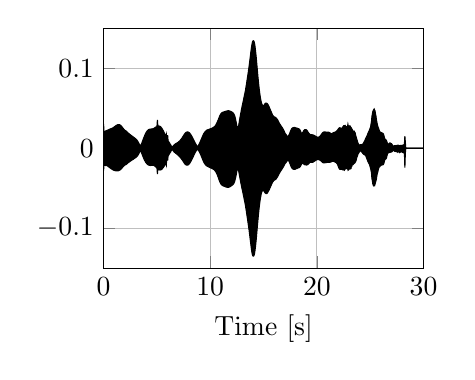
\begin{tikzpicture}

\begin{axis}[%
width=1.6in,
height=1.2in,
at={(0.758in,0.481in)},
scale only axis,
xmin=0,
xmax=30,
xmajorgrids,
ymin=-0.15,
ymax=0.15,
ymajorgrids,
xlabel={Time [s]},
axis background/.style={fill=white}
]
\addplot[fill=black,draw=black,forget plot] plot table[row sep=crcr]{%
2.08333333333333e-05	0.0304416418075562\\
0.0417454218822439	0.0205755233764648\\
0.0834700104311544	0.0206973552703857\\
0.125194598980065	0.0208160877227783\\
0.166919187528975	0.0208245515823364\\
0.208643776077886	0.0217314958572388\\
0.250368364626797	0.021902322769165\\
0.292092953175707	0.0221166610717773\\
0.333817541724618	0.0223733186721802\\
0.375542130273528	0.0225492715835571\\
0.417266718822439	0.0227851867675781\\
0.458991307371349	0.0230562686920166\\
0.50071589592026	0.0233050584793091\\
0.54244048446917	0.0235365629196167\\
0.584165073018081	0.0237956047058105\\
0.625889661566991	0.0240602493286133\\
0.667614250115902	0.0242608785629272\\
0.709338838664812	0.0244194269180298\\
0.751063427213723	0.0246721506118774\\
0.792788015762633	0.0248830318450928\\
0.834512604311544	0.0251603126525879\\
0.876237192860454	0.0254495143890381\\
0.917961781409365	0.0258141756057739\\
0.959686369958275	0.0262215137481689\\
1.00141095850719	0.0266654491424561\\
1.0431355470561	0.0270670652389526\\
1.08486013560501	0.027466893196106\\
1.12658472415392	0.0279065370559692\\
1.16830931270283	0.0283100605010986\\
1.21003390125174	0.0286585092544556\\
1.25175848980065	0.0289767980575562\\
1.29348307834956	0.0292458534240723\\
1.33520766689847	0.0294637680053711\\
1.37693225544738	0.0295345783233643\\
1.41865684399629	0.0294804573059082\\
1.4603814325452	0.0295535326004028\\
1.50210602109411	0.0293903350830078\\
1.54383060964302	0.0291081666946411\\
1.58555519819193	0.0287256240844727\\
1.62727978674084	0.0282242298126221\\
1.66900437528975	0.0275870561599731\\
1.71072896383866	0.0269215106964111\\
1.75245355238758	0.0262309312820435\\
1.79417814093649	0.0255312919616699\\
1.8359027294854	0.0248253345489502\\
1.87762731803431	0.0241572856903076\\
1.91935190658322	0.0235656499862671\\
1.96107649513213	0.0229737758636475\\
2.00280108368104	0.0223948955535889\\
2.04452567222995	0.0220069885253906\\
2.08625026077886	0.0216919183731079\\
2.12797484932777	0.0213944911956787\\
2.16969943787668	0.0208141803741455\\
2.21142402642559	0.020035982131958\\
2.2531486149745	0.0195168256759644\\
2.29487320352341	0.0190584659576416\\
2.33659779207232	0.018627405166626\\
2.37832238062123	0.0181654691696167\\
2.42004696917014	0.0177123546600342\\
2.46177155771905	0.0172709226608276\\
2.50349614626796	0.0168540477752686\\
2.54522073481687	0.0164164304733276\\
2.58694532336579	0.0159929990768433\\
2.6286699119147	0.0155874490737915\\
2.67039450046361	0.0151822566986084\\
2.71211908901252	0.0147244930267334\\
2.75384367756143	0.0143729448318481\\
2.79556826611034	0.0140224695205688\\
2.83729285465925	0.0135433673858643\\
2.87901744320816	0.0131561756134033\\
2.92074203175707	0.0127334594726563\\
2.96246662030598	0.0123034715652466\\
3.00419120885489	0.0118772983551025\\
3.0459157974038	0.0113899707794189\\
3.08764038595271	0.0107975006103516\\
3.12936497450162	0.0101280212402344\\
3.17108956305053	0.00931632518768311\\
3.21281415159944	0.00845897197723389\\
3.25453874014835	0.00745260715484619\\
3.29626332869726	0.00645720958709717\\
3.33798791724618	0.00542366504669189\\
3.37971250579509	0.00438213348388672\\
3.421437094344	0.00376522541046143\\
3.46316168289291	0.00354242324829102\\
3.50488627144182	0.0041576623916626\\
3.54661085999073	0.0051875114440918\\
3.58833544853964	0.00647926330566406\\
3.63006003708855	0.00795924663543701\\
3.67178462563746	0.00941789150238037\\
3.71350921418637	0.0109982490539551\\
3.75523380273528	0.0124752521514893\\
3.79695839128419	0.013885498046875\\
3.8386829798331	0.0152139663696289\\
3.88040756838201	0.0165892839431763\\
3.92213215693092	0.0179152488708496\\
3.96385674547983	0.018954873085022\\
4.00558133402874	0.0199832916259766\\
4.04730592257765	0.0208173990249634\\
4.08903051112656	0.0215780735015869\\
4.13075509967547	0.0221942663192749\\
4.17247968822439	0.0227020978927612\\
4.2142042767733	0.0231285095214844\\
4.25592886532221	0.0234254598617554\\
4.29765345387112	0.0236388444900513\\
4.33937804242003	0.0238243341445923\\
4.38110263096894	0.02387535572052\\
4.42282721951785	0.0239366292953491\\
4.46455180806676	0.0239945650100708\\
4.50627639661567	0.0240663290023804\\
4.54800098516458	0.0241228342056274\\
4.58972557371349	0.024235725402832\\
4.6314501622624	0.0243330001831055\\
4.67317475081131	0.0245382785797119\\
4.71489933936022	0.0248579978942871\\
4.75662392790913	0.0251671075820923\\
4.79834851645804	0.0254679918289185\\
4.84007310500695	0.0258471965789795\\
4.88179769355586	0.0262540578842163\\
4.92352228210478	0.0265989303588867\\
4.96524687065368	0.0268322229385376\\
5.0069714592026	0.0272035598754883\\
5.04869604775151	0.035341739654541\\
5.09042063630042	0.0276316404342651\\
5.13214522484933	0.0277367830276489\\
5.17386981339824	0.0278499126434326\\
5.21559440194715	0.0277067422866821\\
5.25731899049606	0.0275560617446899\\
5.29904357904497	0.0272812843322754\\
5.34076816759388	0.0268198251724243\\
5.38249275614279	0.026267409324646\\
5.4242173446917	0.0255763530731201\\
5.46594193324061	0.0247836112976074\\
5.50766652178952	0.0239511728286743\\
5.54939111033843	0.0229641199111938\\
5.59111569888734	0.0219740867614746\\
5.63284028743625	0.0209484100341797\\
5.67456487598516	0.0197001695632935\\
5.71628946453407	0.0185185670852661\\
5.75801405308299	0.0173077583312988\\
5.7997386416319	0.0160505771636963\\
5.84146323018081	0.0148285627365112\\
5.88318781872972	0.0170928239822388\\
5.92491240727863	0.0102510452270508\\
5.96663699582754	0.00756490230560303\\
6.00836158437645	0.0162675380706787\\
6.05008617292536	0.00904762744903564\\
6.09181076147427	0.00852775573730469\\
6.13353535002318	0.00759625434875488\\
6.17525993857209	0.00673997402191162\\
6.216984527121	0.00572538375854492\\
6.25870911566991	0.00470805168151855\\
6.30043370421882	0.00417613983154297\\
6.34215829276773	0.00275206565856934\\
6.38388288131664	0.00214171409606934\\
6.42560746986555	0.00185716152191162\\
6.46733205841446	0.00207650661468506\\
6.50905664696338	0.00261986255645752\\
6.55078123551229	0.00322556495666504\\
6.5925058240612	0.00384640693664551\\
6.63423041261011	0.00434672832489014\\
6.67595500115902	0.00480437278747559\\
6.71767958970793	0.00523591041564941\\
6.75940417825684	0.00557434558868408\\
6.80112876680575	0.00590431690216064\\
6.84285335535466	0.00622045993804932\\
6.88457794390357	0.00656187534332275\\
6.92630253245248	0.00687277317047119\\
6.96802712100139	0.00725185871124268\\
7.0097517095503	0.00770878791809082\\
7.05147629809921	0.00813186168670654\\
7.09320088664812	0.00863885879516602\\
7.13492547519703	0.00915658473968506\\
7.17665006374594	0.00973570346832275\\
7.21837465229485	0.0103694200515747\\
7.26009924084376	0.0110486745834351\\
7.30182382939268	0.0117988586425781\\
7.34354841794159	0.0125613212585449\\
7.3852730064905	0.0134320259094238\\
7.42699759503941	0.0143027305603027\\
7.46872218358832	0.0151857137680054\\
7.51044677213723	0.0160646438598633\\
7.55217136068614	0.0169401168823242\\
7.59389594923505	0.0177412033081055\\
7.63562053778396	0.0184946060180664\\
7.67734512633287	0.0191444158554077\\
7.71906971488178	0.0196542739868164\\
7.76079430343069	0.0200425386428833\\
7.8025188919796	0.0201977491378784\\
7.84424348052851	0.0203450918197632\\
7.88596806907742	0.0203522443771362\\
7.92769265762633	0.0202186107635498\\
7.96941724617524	0.0199754238128662\\
8.01114183472416	0.0196036100387573\\
8.05286642327307	0.0191268920898438\\
8.09459101182198	0.0185396671295166\\
8.13631560037089	0.0178028345108032\\
8.1780401889198	0.0169855356216431\\
8.21976477746871	0.0161432027816772\\
8.26148936601762	0.0152072906494141\\
8.30321395456653	0.0142226219177246\\
8.34493854311544	0.013161301612854\\
8.38666313166435	0.0120658874511719\\
8.42838772021326	0.0109802484512329\\
8.47011230876217	0.00987720489501953\\
8.51183689731108	0.00877606868743896\\
8.55356148585999	0.00758230686187744\\
8.5952860744089	0.00645220279693604\\
8.63701066295781	0.00545871257781982\\
8.67873525150672	0.00434255599975586\\
8.72045984005563	0.00332629680633545\\
8.76218442860454	0.00236082077026367\\
8.80390901715345	0.00146079063415527\\
8.84563360570237	0.00240540504455566\\
8.88735819425128	0.00340628623962402\\
8.92908278280018	0.00441884994506836\\
8.9708073713491	0.00545454025268555\\
9.01253195989801	0.00663983821868896\\
9.05425654844692	0.00784516334533691\\
9.09598113699583	0.00909745693206787\\
9.13770572554474	0.0104261636734009\\
9.17943031409365	0.0116766691207886\\
9.22115490264256	0.013038158416748\\
9.26287949119147	0.0143606662750244\\
9.30460407974038	0.0156738758087158\\
9.34632866828929	0.0169097185134888\\
9.3880532568382	0.017998218536377\\
9.42977784538711	0.0189611911773682\\
9.47150243393602	0.0198090076446533\\
9.51322702248493	0.0205346345901489\\
9.55495161103384	0.0211423635482788\\
9.59667619958275	0.0216869115829468\\
9.63840078813166	0.0221996307373047\\
9.68012537668058	0.0225818157196045\\
9.72184996522949	0.022830605506897\\
9.7635745537784	0.0230357646942139\\
9.80529914232731	0.0232603549957275\\
9.84702373087622	0.02341628074646\\
9.88874831942513	0.0236028432846069\\
9.93047290797404	0.0238324403762817\\
9.97219749652295	0.0240151882171631\\
10.0139220850719	0.0242545604705811\\
10.0556466736208	0.0244691371917725\\
10.0973712621697	0.0246602296829224\\
10.1390958507186	0.0249108076095581\\
10.1808204392675	0.025188684463501\\
10.2225450278164	0.0254365205764771\\
10.2642696163653	0.0257352590560913\\
10.3059942049142	0.0260748863220215\\
10.3477187934631	0.0264842510223389\\
10.3894433820121	0.0268985033035278\\
10.431167970561	0.0274083614349365\\
10.4728925591099	0.0281081199645996\\
10.5146171476588	0.0289080142974854\\
10.5563417362077	0.0298806428909302\\
10.5980663247566	0.0309303998947144\\
10.6397909133055	0.0319918394088745\\
10.6815155018544	0.0333439111709595\\
10.7232400904033	0.0346348285675049\\
10.7649646789523	0.0360163450241089\\
10.8066892675012	0.0375041961669922\\
10.8484138560501	0.0388745069503784\\
10.890138444599	0.0402292013168335\\
10.9318630331479	0.0413647890090942\\
10.9735876216968	0.0424321889877319\\
11.0153122102457	0.0432573556900024\\
11.0570367987946	0.0438616275787354\\
11.0987613873435	0.0443853139877319\\
11.1404859758924	0.0447015762329102\\
11.1822105644414	0.0449701547622681\\
11.2239351529903	0.0451657772064209\\
11.2656597415392	0.0453695058822632\\
11.3073843300881	0.0454912185668945\\
11.349108918637	0.0456857681274414\\
11.3908335071859	0.045915961265564\\
11.4325580957348	0.0461113452911377\\
11.4742826842837	0.0462311506271362\\
11.5160072728326	0.046398401260376\\
11.5577318613816	0.0465344190597534\\
11.5994564499305	0.0467171669006348\\
11.6411810384794	0.0467969179153442\\
11.6829056270283	0.0467897653579712\\
11.7246302155772	0.0467959642410278\\
11.7663548041261	0.0467188358306885\\
11.808079392675	0.0465661287307739\\
11.8498039812239	0.0464041233062744\\
11.8915285697728	0.0461876392364502\\
11.9332531583217	0.0459423065185547\\
11.9749777468707	0.0456039905548096\\
12.0167023354196	0.0453227758407593\\
12.0584269239685	0.0449830293655396\\
12.1001515125174	0.0446221828460693\\
12.1418761010663	0.0441340208053589\\
12.1836006896152	0.0435006618499756\\
12.2253252781641	0.042561411857605\\
12.267049866713	0.0413339138031006\\
12.3087744552619	0.0397731065750122\\
12.3504990438108	0.0376864671707153\\
12.3922236323598	0.03521728515625\\
12.4339482209087	0.0324369668960571\\
12.4756728094576	0.0295660495758057\\
12.5173973980065	0.0266424417495728\\
12.5591219865554	0.0243571996688843\\
12.6008465751043	0.0241470336914063\\
12.6425711636532	0.0265214443206787\\
12.6842957522021	0.029747486114502\\
12.726020340751	0.0333627462387085\\
12.7677449293	0.0366218090057373\\
12.8094695178489	0.0397109985351563\\
12.8511941063978	0.0427742004394531\\
12.8929186949467	0.0457028150558472\\
12.9346432834956	0.0486544370651245\\
12.9763678720445	0.0514482259750366\\
13.0180924605934	0.0540609359741211\\
13.0598170491423	0.0566239356994629\\
13.1015416376912	0.0592532157897949\\
13.1432662262401	0.0620166063308716\\
13.1849908147891	0.064704418182373\\
13.226715403338	0.0674242973327637\\
13.2684399918869	0.0699965953826904\\
13.3101645804358	0.0728389024734497\\
13.3518891689847	0.0764144659042358\\
13.3936137575336	0.0796667337417603\\
13.4353383460825	0.0835342407226563\\
13.4770629346314	0.0871860980987549\\
13.5187875231803	0.0907418727874756\\
13.5605121117293	0.0943212509155273\\
13.6022367002782	0.0983403921127319\\
13.6439612888271	0.102481126785278\\
13.685685877376	0.106798648834229\\
13.7274104659249	0.111116051673889\\
13.7691350544738	0.115838050842285\\
13.8108596430227	0.120370864868164\\
13.8525842315716	0.124593138694763\\
13.8943088201205	0.128315806388855\\
13.9360334086694	0.131450772285461\\
13.9777579972184	0.133512258529663\\
14.0194825857673	0.13420569896698\\
14.0612071743162	0.134293794631958\\
14.1029317628651	0.133555293083191\\
14.144656351414	0.131409049034119\\
14.1863809399629	0.12833833694458\\
14.2281055285118	0.124110817909241\\
14.2698301170607	0.118898034095764\\
14.3115547056096	0.113546848297119\\
14.3532792941586	0.107146620750427\\
14.3950038827075	0.101034879684448\\
14.4367284712564	0.094620943069458\\
14.4784530598053	0.0885579586029053\\
14.5201776483542	0.0828765630722046\\
14.5619022369031	0.077487587928772\\
14.603626825452	0.0725328922271729\\
14.6453514140009	0.0684523582458496\\
14.6870760025498	0.0644452571868896\\
14.7288005910988	0.061158299446106\\
14.7705251796477	0.0584886074066162\\
14.8122497681966	0.056445837020874\\
14.8539743567455	0.0549070835113525\\
14.8956989452944	0.053713321685791\\
14.9374235338433	0.0531024932861328\\
14.9791481223922	0.05320143699646\\
15.0208727109411	0.0536360740661621\\
15.06259729949	0.0542856454849243\\
15.1043218880389	0.0551272630691528\\
15.1460464765879	0.0557597875595093\\
15.1877710651368	0.0563288927078247\\
15.2294956536857	0.0563076734542847\\
15.2712202422346	0.0562951564788818\\
15.3129448307835	0.0561478137969971\\
15.3546694193324	0.0555846691131592\\
15.3963940078813	0.0548645257949829\\
15.4381185964302	0.0539151430130005\\
15.4798431849791	0.0528358221054077\\
15.521567773528	0.0516059398651123\\
15.563292362077	0.0503354072570801\\
15.6050169506259	0.0489121675491333\\
15.6467415391748	0.0476671457290649\\
15.6884661277237	0.0463520288467407\\
15.7301907162726	0.0449930429458618\\
15.7719153048215	0.0436943769454956\\
15.8136398933704	0.0424467325210571\\
15.8553644819193	0.0413386821746826\\
15.8970890704682	0.0404732227325439\\
15.9388136590172	0.0398648977279663\\
15.9805382475661	0.0393712520599365\\
16.022262836115	0.0390514135360718\\
16.0639874246639	0.0388305187225342\\
16.1057120132128	0.0385569334030151\\
16.1474366017617	0.0382198095321655\\
16.1891611903106	0.0377428531646729\\
16.2308857788595	0.0370118618011475\\
16.2726103674084	0.0362670421600342\\
16.3143349559573	0.0354539155960083\\
16.3560595445063	0.0342915058135986\\
16.3977841330552	0.033247709274292\\
16.4395087216041	0.0322955846786499\\
16.481233310153	0.0312085151672363\\
16.5229578987019	0.0302096605300903\\
16.5646824872508	0.0294233560562134\\
16.6064070757997	0.028465747833252\\
16.6481316643486	0.0276988744735718\\
16.6898562528975	0.026874303817749\\
16.7315808414465	0.026124119758606\\
16.7733054299954	0.0252689123153687\\
16.8150300185443	0.0242857933044434\\
16.8567546070932	0.023195743560791\\
16.8984791956421	0.0222135782241821\\
16.940203784191	0.0209852457046509\\
16.9819283727399	0.0196859836578369\\
17.0236529612888	0.0185569524765015\\
17.0653775498377	0.017784595489502\\
17.1071021383867	0.0170919895172119\\
17.1488267269356	0.0161497592926025\\
17.1905513154845	0.0154000520706177\\
17.2322759040334	0.0148926973342896\\
17.2740004925823	0.0145163536071777\\
17.3157250811312	0.0149081945419312\\
17.3574496696801	0.0158184766769409\\
17.399174258229	0.0170267820358276\\
17.4408988467779	0.0183608531951904\\
17.4826234353268	0.0196834802627563\\
17.5243480238758	0.0210748910903931\\
17.5660726124247	0.0224505662918091\\
17.6077972009736	0.0235865116119385\\
17.6495217895225	0.0245461463928223\\
17.6912463780714	0.0252125263214111\\
17.7329709666203	0.0254424810409546\\
17.7746955551692	0.0256786346435547\\
17.8164201437181	0.0258268117904663\\
17.858144732267	0.0259511470794678\\
17.8998693208159	0.0259764194488525\\
17.9415939093649	0.0258368253707886\\
17.9833184979138	0.0256180763244629\\
18.0250430864627	0.0252213478088379\\
18.0667676750116	0.0252730846405029\\
18.1084922635605	0.0251896381378174\\
18.1502168521094	0.0251016616821289\\
18.1919414406583	0.0245758295059204\\
18.2336660292072	0.0245085954666138\\
18.2753906177561	0.0243923664093018\\
18.3171152063051	0.0241373777389526\\
18.358839794854	0.023733377456665\\
18.4005643834029	0.0230120420455933\\
18.4422889719518	0.0219981670379639\\
18.4840135605007	0.0207706689834595\\
18.5257381490496	0.0194844007492065\\
18.5674627375985	0.0183166265487671\\
18.6091873261474	0.0184763669967651\\
18.6509119146963	0.0192369222640991\\
18.6926365032453	0.0201106071472168\\
18.7343610917942	0.0210824012756348\\
18.7760856803431	0.0220675468444824\\
18.817810268892	0.0227826833724976\\
18.8595348574409	0.023165225982666\\
18.9012594459898	0.0232583284378052\\
18.9429840345387	0.0232406854629517\\
18.9847086230876	0.0231567621231079\\
19.0264332116365	0.0229698419570923\\
19.0681578001854	0.0222688913345337\\
19.1098823887344	0.0214753150939941\\
19.1516069772833	0.0205174684524536\\
19.1933315658322	0.0195932388305664\\
19.2350561543811	0.0188281536102295\\
19.27678074293	0.0182381868362427\\
19.3185053314789	0.0175942182540894\\
19.3602299200278	0.01703941822052\\
19.4019545085767	0.0168997049331665\\
19.4436790971256	0.0168880224227905\\
19.4854036856745	0.0168882608413696\\
19.5271282742235	0.0168646574020386\\
19.5688528627724	0.0167956352233887\\
19.6105774513213	0.0167096853256226\\
19.6523020398702	0.0165278911590576\\
19.6940266284191	0.0163141489028931\\
19.735751216968	0.0160030126571655\\
19.7774758055169	0.0157508850097656\\
19.8192003940658	0.0154117345809937\\
19.8609249826147	0.0150964260101318\\
19.9026495711637	0.0147551298141479\\
19.9443741597126	0.0144549608230591\\
19.9860987482615	0.0141996145248413\\
20.0278233368104	0.0139071941375732\\
20.0695479253593	0.0138683319091797\\
20.1112725139082	0.0138165950775146\\
20.1529971024571	0.0138221979141235\\
20.194721691006	0.0141096115112305\\
20.2364462795549	0.0144225358963013\\
20.2781708681038	0.0148519277572632\\
20.3198954566528	0.0154272317886353\\
20.3616200452017	0.0161932706832886\\
20.4033446337506	0.0169275999069214\\
20.4450692222995	0.0177420377731323\\
20.4867938108484	0.0185669660568237\\
20.5285183993973	0.0191744565963745\\
20.5702429879462	0.0198047161102295\\
20.6119675764951	0.0200843811035156\\
20.653692165044	0.0202674865722656\\
20.695416753593	0.0202670097351074\\
20.7371413421419	0.020307183265686\\
20.7788659306908	0.0203179121017456\\
20.8205905192397	0.0201915502548218\\
20.8623151077886	0.0201315879821777\\
20.9040396963375	0.0201107263565063\\
20.9457642848864	0.0201224088668823\\
20.9874888734353	0.0201027393341064\\
21.0292134619842	0.0200297832489014\\
21.0709380505331	0.0199867486953735\\
21.1126626390821	0.0199021100997925\\
21.154387227631	0.0197861194610596\\
21.1961118161799	0.0195039510726929\\
21.2378364047288	0.0191242694854736\\
21.2795609932777	0.0186479091644287\\
21.3212855818266	0.018062949180603\\
21.3630101703755	0.0178283452987671\\
21.4047347589244	0.0181642770767212\\
21.4464593474733	0.0185797214508057\\
21.4881839360223	0.0189753770828247\\
21.5299085245712	0.0192364454269409\\
21.5716331131201	0.0195285081863403\\
21.613357701669	0.0197669267654419\\
21.6550822902179	0.0199398994445801\\
21.6968068787668	0.0200281143188477\\
21.7385314673157	0.0202833414077759\\
21.7802560558646	0.0207023620605469\\
21.8219806444135	0.0210205316543579\\
21.8637052329624	0.0215293169021606\\
21.9054298215114	0.0221596956253052\\
21.9471544100603	0.0228894948959351\\
21.9888789986092	0.0237751007080078\\
22.0306035871581	0.0245027542114258\\
22.072328175707	0.0252293348312378\\
22.1140527642559	0.025551438331604\\
22.1557773528048	0.0256205797195435\\
22.1975019413537	0.0252020359039307\\
22.2392265299026	0.0249272584915161\\
22.2809511184516	0.024474024772644\\
22.3226757070005	0.0249930620193481\\
22.3644002955494	0.0252747535705566\\
22.4061248840983	0.0263153314590454\\
22.4478494726472	0.0264471769332886\\
22.4895740611961	0.0279123783111572\\
22.531298649745	0.0275607109069824\\
22.5730232382939	0.0282152891159058\\
22.6147478268428	0.0276670455932617\\
22.6564724153917	0.0282759666442871\\
22.6981970039407	0.0270742177963257\\
22.7399215924896	0.0268223285675049\\
22.7816461810385	0.0263811349868774\\
22.8233707695874	0.0270346403121948\\
22.8650953581363	0.0267759561538696\\
22.9068199466852	0.0297988653182983\\
22.9485445352341	0.0268460512161255\\
22.990269123783	0.0276384353637695\\
23.0319937123319	0.0279824733734131\\
23.0737183008809	0.0277848243713379\\
23.1154428894298	0.027789831161499\\
23.1571674779787	0.0265239477157593\\
23.1988920665276	0.0259915590286255\\
23.2406166550765	0.0247836112976074\\
23.2823412436254	0.0240364074707031\\
23.3240658321743	0.0229761600494385\\
23.3657904207232	0.0216997861862183\\
23.4075150092721	0.021467924118042\\
23.449239597821	0.0209184885025024\\
23.49096418637	0.0213030576705933\\
23.5326887749189	0.0198565721511841\\
23.5744133634678	0.0197092294692993\\
23.6161379520167	0.017151951789856\\
23.6578625405656	0.0150809288024902\\
23.6995871291145	0.0131478309631348\\
23.7413117176634	0.0112348794937134\\
23.7830363062123	0.00948715209960938\\
23.8247608947612	0.0074927806854248\\
23.8664854833102	0.00584959983825684\\
23.9082100718591	0.00490999221801758\\
23.949934660408	0.00362277030944824\\
23.9916592489569	0.0039207935333252\\
24.0333838375058	0.00422787666320801\\
24.0751084260547	0.00446438789367676\\
24.1168330146036	0.00450229644775391\\
24.1585576031525	0.00463330745697021\\
24.2002821917014	0.00453031063079834\\
24.2420067802503	0.00453543663024902\\
24.2837313687993	0.00484704971313477\\
24.3254559573482	0.005615234375\\
24.3671805458971	0.00643253326416016\\
24.408905134446	0.00734031200408936\\
24.4506297229949	0.00840270519256592\\
24.4923543115438	0.00943481922149658\\
24.5340789000927	0.0108433961868286\\
24.5758034886416	0.0122237205505371\\
24.6175280771905	0.0134420394897461\\
24.6592526657395	0.0143798589706421\\
24.7009772542884	0.0154467821121216\\
24.7427018428373	0.0168440341949463\\
24.7844264313862	0.0184445381164551\\
24.8261510199351	0.0200291872024536\\
24.867875608484	0.0207918882369995\\
24.9096001970329	0.0219243764877319\\
24.9513247855818	0.0236788988113403\\
24.9930493741307	0.0249984264373779\\
25.0347739626796	0.0265214443206787\\
25.0764985512286	0.03026282787323\\
25.1182231397775	0.0329892635345459\\
25.1599477283264	0.0400756597518921\\
25.2016723168753	0.0422376394271851\\
25.2433969054242	0.0459668636322021\\
25.2851214939731	0.0470137596130371\\
25.326846082522	0.048227071762085\\
25.3685706710709	0.0490291118621826\\
25.4102952596198	0.0476396083831787\\
25.4520198481687	0.0465965270996094\\
25.4937444367177	0.0426558256149292\\
25.5354690252666	0.0403163433074951\\
25.5771936138155	0.0362153053283691\\
25.6189182023644	0.0326656103134155\\
25.6606427909133	0.0302164554595947\\
25.7023673794622	0.0275977849960327\\
25.7440919680111	0.0258979797363281\\
25.78581655656	0.0247557163238525\\
25.8275411451089	0.0230933427810669\\
25.8692657336579	0.021365761756897\\
25.9109903222068	0.0205650329589844\\
25.9527149107557	0.0198453664779663\\
25.9944394993046	0.0198585987091064\\
26.0361640878535	0.0196374654769897\\
26.0778886764024	0.0192607641220093\\
26.1196132649513	0.0189319849014282\\
26.1613378535002	0.018796443939209\\
26.2030624420491	0.0184100866317749\\
26.2447870305981	0.017504096031189\\
26.286511619147	0.0155837535858154\\
26.3282362076959	0.0134836435317993\\
26.3699607962448	0.0117475986480713\\
26.4116853847937	0.011044979095459\\
26.4534099733426	0.0108481645584106\\
26.4951345618915	0.0101442337036133\\
26.5368591504404	0.00912868976593018\\
26.5785837389893	0.00747597217559814\\
26.6203083275383	0.00518584251403809\\
26.6620329160872	0.00530588626861572\\
26.7037575046361	0.0053105354309082\\
26.745482093185	0.00552117824554443\\
26.7872066817339	0.00599026679992676\\
26.8289312702828	0.00650596618652344\\
26.8706558588317	0.00654232501983643\\
26.9123804473806	0.00611031055450439\\
26.9541050359295	0.00567936897277832\\
26.9958296244784	0.00559043884277344\\
27.0375542130274	0.00493705272674561\\
27.0792788015763	0.003875732421875\\
27.1210033901252	0.00302672386169434\\
27.1627279786741	0.00248467922210693\\
27.204452567223	0.00270211696624756\\
27.2461771557719	0.00304365158081055\\
27.2879017443208	0.00312924385070801\\
27.3296263328697	0.0030968189239502\\
27.3713509214186	0.00295281410217285\\
27.4130755099675	0.00334548950195313\\
27.4548000985165	0.00347065925598145\\
27.4965246870654	0.00312185287475586\\
27.5382492756143	0.00274455547332764\\
27.5799738641632	0.00380051136016846\\
27.6216984527121	0.0038982629776001\\
27.663423041261	0.00350356101989746\\
27.7051476298099	0.0033336877822876\\
27.7468722183588	0.00311505794525146\\
27.7885968069077	0.00319516658782959\\
27.8303213954567	0.00348269939422607\\
27.8720459840056	0.00309967994689941\\
27.9137705725545	0.00331568717956543\\
27.9554951611034	0.00351893901824951\\
27.9972197496523	0.00373303890228271\\
28.0389443382012	0.00364625453948975\\
28.0806689267501	0.0039595365524292\\
28.122393515299	0.00409936904907227\\
28.1641181038479	0.00442612171173096\\
28.2058426923968	0.00486993789672852\\
28.2475672809458	0.0150246620178223\\
28.2892918694947	0.00800168514251709\\
28.3310164580436	0.00032508373260498\\
28.3727410465925	0.000179767608642578\\
28.4144656351414	0.000209808349609375\\
28.4561902236903	0.000157356262207031\\
28.4979148122392	0.000116944313049316\\
28.5396394007881	7.05718994140625e-05\\
28.581363989337	1.12056732177734e-05\\
28.623088577886	-7.98702239990234e-06\\
28.6648131664349	-4.87565994262695e-05\\
28.7065377549838	2.46763229370117e-05\\
28.7482623435327	8.96453857421875e-05\\
28.7899869320816	0.000128507614135742\\
28.8317115206305	0.000129461288452148\\
28.8734361091794	0.00010526180267334\\
28.9151606977283	9.19103622436523e-05\\
28.9568852862772	5.88893890380859e-05\\
28.9986098748261	6.43730163574219e-05\\
29.0403344633751	5.80549240112305e-05\\
29.082059051924	6.27040863037109e-05\\
29.1237836404729	4.72068786621094e-05\\
29.1655082290218	6.00814819335938e-05\\
29.2072328175707	7.10487365722656e-05\\
29.2489574061196	6.77108764648438e-05\\
29.2906819946685	6.00814819335938e-05\\
29.3324065832174	5.18560409545898e-05\\
29.3741311717663	6.04391098022461e-05\\
29.4158557603153	5.80549240112305e-05\\
29.4575803488642	4.22000885009766e-05\\
29.4993049374131	6.29425048828125e-05\\
29.541029525962	5.340576171875e-05\\
29.5827541145109	5.96046447753906e-05\\
29.6244787030598	5.30481338500977e-05\\
29.6662032916087	6.54458999633789e-05\\
29.7079278801576	6.27040863037109e-05\\
29.7496524687065	5.92470169067383e-05\\
29.7913770572554	6.25848770141602e-05\\
29.8331016458044	4.38690185546875e-05\\
29.8748262343533	5.55515289306641e-05\\
29.9165508229022	4.8518180847168e-05\\
29.9582754114511	6.27040863037109e-05\\
30	5.68628311157227e-05\\
}
\closedcycle;
\addplot[fill=black,draw=black,forget plot] plot table[row sep=crcr]{%
2.08333333333333e-05	-0.0280479192733765\\
0.0417454218822439	-0.0210698843002319\\
0.0834700104311544	-0.0212905406951904\\
0.125194598980065	-0.0214548110961914\\
0.166919187528975	-0.0216097831726074\\
0.208643776077886	-0.0216915607452393\\
0.250368364626797	-0.0212579965591431\\
0.292092953175707	-0.0215262174606323\\
0.333817541724618	-0.0219072103500366\\
0.375542130273528	-0.0222067832946777\\
0.417266718822439	-0.0226218700408936\\
0.458991307371349	-0.0231003761291504\\
0.50071589592026	-0.0234450101852417\\
0.54244048446917	-0.0239048004150391\\
0.584165073018081	-0.024286150932312\\
0.625889661566991	-0.0247431993484497\\
0.667614250115902	-0.025076150894165\\
0.709338838664812	-0.0256001949310303\\
0.751063427213723	-0.0259400606155396\\
0.792788015762633	-0.0262843370437622\\
0.834512604311544	-0.026645302772522\\
0.876237192860454	-0.0269436836242676\\
0.917961781409365	-0.0271997451782227\\
0.959686369958275	-0.0274542570114136\\
1.00141095850719	-0.0276824235916138\\
1.0431355470561	-0.0279031991958618\\
1.08486013560501	-0.0280325412750244\\
1.12658472415392	-0.0281280279159546\\
1.16830931270283	-0.0282211303710938\\
1.21003390125174	-0.0283212661743164\\
1.25175848980065	-0.0283174514770508\\
1.29348307834956	-0.0283491611480713\\
1.33520766689847	-0.0283030271530151\\
1.37693225544738	-0.0281673669815063\\
1.41865684399629	-0.0279737710952759\\
1.4603814325452	-0.0277680158615112\\
1.50210602109411	-0.0274744033813477\\
1.54383060964302	-0.0271122455596924\\
1.58555519819193	-0.0266915559768677\\
1.62727978674084	-0.0261778831481934\\
1.66900437528975	-0.0255833864212036\\
1.71072896383866	-0.0250129699707031\\
1.75245355238758	-0.0243679285049438\\
1.79417814093649	-0.0237735509872437\\
1.8359027294854	-0.0231204032897949\\
1.87762731803431	-0.0225385427474976\\
1.91935190658322	-0.0219759941101074\\
1.96107649513213	-0.0214921236038208\\
2.00280108368104	-0.0210548639297485\\
2.04452567222995	-0.0206871032714844\\
2.08625026077886	-0.0204759836196899\\
2.12797484932777	-0.0202486515045166\\
2.16969943787668	-0.0198180675506592\\
2.21142402642559	-0.0191413164138794\\
2.2531486149745	-0.0187269449234009\\
2.29487320352341	-0.0182245969772339\\
2.33659779207232	-0.0178340673446655\\
2.37832238062123	-0.0174582004547119\\
2.42004696917014	-0.0170572996139526\\
2.46177155771905	-0.0166534185409546\\
2.50349614626796	-0.0162390470504761\\
2.54522073481687	-0.0158693790435791\\
2.58694532336579	-0.0155093669891357\\
2.6286699119147	-0.0151301622390747\\
2.67039450046361	-0.014757513999939\\
2.71211908901252	-0.0143957138061523\\
2.75384367756143	-0.0141454935073853\\
2.79556826611034	-0.0136857032775879\\
2.83729285465925	-0.0132796764373779\\
2.87901744320816	-0.0128598213195801\\
2.92074203175707	-0.0124876499176025\\
2.96246662030598	-0.012153148651123\\
3.00419120885489	-0.0117292404174805\\
3.0459157974038	-0.0113143920898438\\
3.08764038595271	-0.0108308792114258\\
3.12936497450162	-0.0103135108947754\\
3.17108956305053	-0.00959968566894531\\
3.21281415159944	-0.00885701179504395\\
3.25453874014835	-0.00801587104797363\\
3.29626332869726	-0.00703823566436768\\
3.33798791724618	-0.00588583946228027\\
3.37971250579509	-0.00462579727172852\\
3.421437094344	-0.00340175628662109\\
3.46316168289291	-0.00247085094451904\\
3.50488627144182	-0.00375807285308838\\
3.54661085999073	-0.00519609451293945\\
3.58833544853964	-0.0066673755645752\\
3.63006003708855	-0.00815188884735107\\
3.67178462563746	-0.00961768627166748\\
3.71350921418637	-0.010982871055603\\
3.75523380273528	-0.0124185085296631\\
3.79695839128419	-0.0136414766311646\\
3.8386829798331	-0.0147758722305298\\
3.88040756838201	-0.01585853099823\\
3.92213215693092	-0.0168486833572388\\
3.96385674547983	-0.0177270174026489\\
4.00558133402874	-0.0184720754623413\\
4.04730592257765	-0.0191431045532227\\
4.08903051112656	-0.0197271108627319\\
4.13075509967547	-0.0202215909957886\\
4.17247968822439	-0.0206488370895386\\
4.2142042767733	-0.0209774971008301\\
4.25592886532221	-0.0212588310241699\\
4.29765345387112	-0.021392822265625\\
4.33937804242003	-0.0214740037918091\\
4.38110263096894	-0.0215433835983276\\
4.42282721951785	-0.0215163230895996\\
4.46455180806676	-0.0215132236480713\\
4.50627639661567	-0.0214987993240356\\
4.54800098516458	-0.0214653015136719\\
4.58972557371349	-0.02141273021698\\
4.6314501622624	-0.0213606357574463\\
4.67317475081131	-0.0214235782623291\\
4.71489933936022	-0.0216238498687744\\
4.75662392790913	-0.0218883752822876\\
4.79834851645804	-0.0222598314285278\\
4.84007310500695	-0.022607684135437\\
4.88179769355586	-0.0230779647827148\\
4.92352228210478	-0.0236308574676514\\
4.96524687065368	-0.0241477489471436\\
5.0069714592026	-0.024660587310791\\
5.04869604775151	-0.0321727991104126\\
5.09042063630042	-0.0258612632751465\\
5.13214522484933	-0.0263245105743408\\
5.17386981339824	-0.0266907215118408\\
5.21559440194715	-0.0270445346832275\\
5.25731899049606	-0.0271563529968262\\
5.29904357904497	-0.0271850824356079\\
5.34076816759388	-0.0271137952804565\\
5.38249275614279	-0.0269118547439575\\
5.4242173446917	-0.026666522026062\\
5.46594193324061	-0.0261284112930298\\
5.50766652178952	-0.0256038904190063\\
5.54939111033843	-0.0249019861221313\\
5.59111569888734	-0.0242290496826172\\
5.63284028743625	-0.0234725475311279\\
5.67456487598516	-0.0225805044174194\\
5.71628946453407	-0.0216242074966431\\
5.75801405308299	-0.0205742120742798\\
5.7997386416319	-0.0194700956344604\\
5.84146323018081	-0.0182554721832275\\
5.88318781872972	-0.0206520557403564\\
5.92491240727863	-0.0114001035690308\\
5.96663699582754	-0.00861084461212158\\
6.00836158437645	-0.0155609846115112\\
6.05008617292536	-0.00912487506866455\\
6.09181076147427	-0.00881648063659668\\
6.13353535002318	-0.00763416290283203\\
6.17525993857209	-0.00696325302124023\\
6.216984527121	-0.00596308708190918\\
6.25870911566991	-0.00496339797973633\\
6.30043370421882	-0.00454950332641602\\
6.34215829276773	-0.00301539897918701\\
6.38388288131664	-0.00217330455780029\\
6.42560746986555	-0.00162434577941895\\
6.46733205841446	-0.00214910507202148\\
6.50905664696338	-0.00290107727050781\\
6.55078123551229	-0.00356566905975342\\
6.5925058240612	-0.00423157215118408\\
6.63423041261011	-0.00479614734649658\\
6.67595500115902	-0.00533628463745117\\
6.71767958970793	-0.00579822063446045\\
6.75940417825684	-0.00621795654296875\\
6.80112876680575	-0.00668275356292725\\
6.84285335535466	-0.00707244873046875\\
6.88457794390357	-0.00742840766906738\\
6.92630253245248	-0.00796067714691162\\
6.96802712100139	-0.00842380523681641\\
7.0097517095503	-0.00891256332397461\\
7.05147629809921	-0.00942349433898926\\
7.09320088664812	-0.00999653339385986\\
7.13492547519703	-0.0105726718902588\\
7.17665006374594	-0.0111842155456543\\
7.21837465229485	-0.0118539333343506\\
7.26009924084376	-0.0125198364257813\\
7.30182382939268	-0.0132988691329956\\
7.34354841794159	-0.0140731334686279\\
7.3852730064905	-0.0148242712020874\\
7.42699759503941	-0.0156879425048828\\
7.46872218358832	-0.01652991771698\\
7.51044677213723	-0.0173740386962891\\
7.55217136068614	-0.0182335376739502\\
7.59389594923505	-0.019025444984436\\
7.63562053778396	-0.0197255611419678\\
7.67734512633287	-0.0202990770339966\\
7.71906971488178	-0.020740270614624\\
7.76079430343069	-0.0210108757019043\\
7.8025188919796	-0.0211156606674194\\
7.84424348052851	-0.0211502313613892\\
7.88596806907742	-0.0210576057434082\\
7.92769265762633	-0.0207697153091431\\
7.96941724617524	-0.0203889608383179\\
8.01114183472416	-0.0198168754577637\\
8.05286642327307	-0.0191692113876343\\
8.09459101182198	-0.0183824300765991\\
8.13631560037089	-0.0175144672393799\\
8.1780401889198	-0.0165579319000244\\
8.21976477746871	-0.0155677795410156\\
8.26148936601762	-0.0145046710968018\\
8.30321395456653	-0.0133969783782959\\
8.34493854311544	-0.012253999710083\\
8.38666313166435	-0.0110890865325928\\
8.42838772021326	-0.00985908508300781\\
8.47011230876217	-0.00861001014709473\\
8.51183689731108	-0.00742626190185547\\
8.55356148585999	-0.00634229183197021\\
8.5952860744089	-0.00525164604187012\\
8.63701066295781	-0.00418853759765625\\
8.67873525150672	-0.0033266544342041\\
8.72045984005563	-0.00266897678375244\\
8.76218442860454	-0.00214993953704834\\
8.80390901715345	-0.00178992748260498\\
8.84563360570237	-0.00186336040496826\\
8.88735819425128	-0.00244367122650146\\
8.92908278280018	-0.00327765941619873\\
8.9708073713491	-0.00420284271240234\\
9.01253195989801	-0.00527381896972656\\
9.05425654844692	-0.00641405582427979\\
9.09598113699583	-0.00770330429077148\\
9.13770572554474	-0.00896251201629639\\
9.17943031409365	-0.0104153156280518\\
9.22115490264256	-0.0117956399917603\\
9.26287949119147	-0.0131698846817017\\
9.30460407974038	-0.0145969390869141\\
9.34632866828929	-0.015933632850647\\
9.3880532568382	-0.0171345472335815\\
9.42977784538711	-0.0181550979614258\\
9.47150243393602	-0.0190980434417725\\
9.51322702248493	-0.019843578338623\\
9.55495161103384	-0.0205657482147217\\
9.59667619958275	-0.0211632251739502\\
9.63840078813166	-0.0217099189758301\\
9.68012537668058	-0.0221182107925415\\
9.72184996522949	-0.0224678516387939\\
9.7635745537784	-0.0227557420730591\\
9.80529914232731	-0.0230311155319214\\
9.84702373087622	-0.0232810974121094\\
9.88874831942513	-0.023525595664978\\
9.93047290797404	-0.0237977504730225\\
9.97219749652295	-0.0240676403045654\\
10.0139220850719	-0.0243237018585205\\
10.0556466736208	-0.0246609449386597\\
10.0973712621697	-0.0248441696166992\\
10.1390958507186	-0.0250502824783325\\
10.1808204392675	-0.0253393650054932\\
10.2225450278164	-0.0256969928741455\\
10.2642696163653	-0.0260581970214844\\
10.3059942049142	-0.0263557434082031\\
10.3477187934631	-0.0266406536102295\\
10.3894433820121	-0.0271471738815308\\
10.431167970561	-0.0277456045150757\\
10.4728925591099	-0.0285148620605469\\
10.5146171476588	-0.0293327569961548\\
10.5563417362077	-0.0302385091781616\\
10.5980663247566	-0.0312831401824951\\
10.6397909133055	-0.032591700553894\\
10.6815155018544	-0.0338271856307983\\
10.7232400904033	-0.0354197025299072\\
10.7649646789523	-0.0370017290115356\\
10.8066892675012	-0.0387203693389893\\
10.8484138560501	-0.0402191877365112\\
10.890138444599	-0.0416790246963501\\
10.9318630331479	-0.0429623126983643\\
10.9735876216968	-0.044026255607605\\
11.0153122102457	-0.0448904037475586\\
11.0570367987946	-0.0455948114395142\\
11.0987613873435	-0.0461032390594482\\
11.1404859758924	-0.0464818477630615\\
11.1822105644414	-0.0468076467514038\\
11.2239351529903	-0.0471063852310181\\
11.2656597415392	-0.0472182035446167\\
11.3073843300881	-0.0474939346313477\\
11.349108918637	-0.0477652549743652\\
11.3908335071859	-0.0479941368103027\\
11.4325580957348	-0.0481935739517212\\
11.4742826842837	-0.0484206676483154\\
11.5160072728326	-0.0486105680465698\\
11.5577318613816	-0.0486909151077271\\
11.5994564499305	-0.0487761497497559\\
11.6411810384794	-0.048795223236084\\
11.6829056270283	-0.048754096031189\\
11.7246302155772	-0.0487356185913086\\
11.7663548041261	-0.0486301183700562\\
11.808079392675	-0.0483587980270386\\
11.8498039812239	-0.0481269359588623\\
11.8915285697728	-0.0477243661880493\\
11.9332531583217	-0.0474039316177368\\
11.9749777468707	-0.0469892024993896\\
12.0167023354196	-0.0465819835662842\\
12.0584269239685	-0.0461983680725098\\
12.1001515125174	-0.0457577705383301\\
12.1418761010663	-0.0452392101287842\\
12.1836006896152	-0.0445761680603027\\
12.2253252781641	-0.0436007976531982\\
12.267049866713	-0.0423110723495483\\
12.3087744552619	-0.0405895709991455\\
12.3504990438108	-0.038476824760437\\
12.3922236323598	-0.035957932472229\\
12.4339482209087	-0.0332013368606567\\
12.4756728094576	-0.0303114652633667\\
12.5173973980065	-0.0274301767349243\\
12.5591219865554	-0.0252090692520142\\
12.6008465751043	-0.0248124599456787\\
12.6425711636532	-0.0267767906188965\\
12.6842957522021	-0.02955162525177\\
12.726020340751	-0.0327035188674927\\
12.7677449293	-0.035901665687561\\
12.8094695178489	-0.0387609004974365\\
12.8511941063978	-0.0418263673782349\\
12.8929186949467	-0.0447230339050293\\
12.9346432834956	-0.0475324392318726\\
12.9763678720445	-0.0502169132232666\\
13.0180924605934	-0.0528099536895752\\
13.0598170491423	-0.0553629398345947\\
13.1015416376912	-0.0579632520675659\\
13.1432662262401	-0.0607507228851318\\
13.1849908147891	-0.0635086297988892\\
13.226715403338	-0.0664997100830078\\
13.2684399918869	-0.0690327882766724\\
13.3101645804358	-0.0722241401672363\\
13.3518891689847	-0.0758695602416992\\
13.3936137575336	-0.0793901681900024\\
13.4353383460825	-0.0832116603851318\\
13.4770629346314	-0.0869382619857788\\
13.5187875231803	-0.0906350612640381\\
13.5605121117293	-0.0944876670837402\\
13.6022367002782	-0.0983983278274536\\
13.6439612888271	-0.102569460868835\\
13.685685877376	-0.10689651966095\\
13.7274104659249	-0.111605167388916\\
13.7691350544738	-0.116201400756836\\
13.8108596430227	-0.120694875717163\\
13.8525842315716	-0.12505829334259\\
13.8943088201205	-0.128980278968811\\
13.9360334086694	-0.132103681564331\\
13.9777579972184	-0.134125113487244\\
14.0194825857673	-0.134864091873169\\
14.0612071743162	-0.134835004806519\\
14.1029317628651	-0.134075164794922\\
14.144656351414	-0.131953001022339\\
14.1863809399629	-0.128798007965088\\
14.2281055285118	-0.124505877494812\\
14.2698301170607	-0.119434952735901\\
14.3115547056096	-0.113879323005676\\
14.3532792941586	-0.107648372650146\\
14.3950038827075	-0.101232647895813\\
14.4367284712564	-0.0949821472167969\\
14.4784530598053	-0.088822603225708\\
14.5201776483542	-0.0828280448913574\\
14.5619022369031	-0.0774605274200439\\
14.603626825452	-0.0725196599960327\\
14.6453514140009	-0.0680360794067383\\
14.6870760025498	-0.0639787912368774\\
14.7288005910988	-0.0607854127883911\\
14.7705251796477	-0.0577890872955322\\
14.8122497681966	-0.0555657148361206\\
14.8539743567455	-0.0539628267288208\\
14.8956989452944	-0.0531870126724243\\
14.9374235338433	-0.0527787208557129\\
14.9791481223922	-0.0528196096420288\\
15.0208727109411	-0.0532976388931274\\
15.06259729949	-0.0541996955871582\\
15.1043218880389	-0.0550053119659424\\
15.1460464765879	-0.0557972192764282\\
15.1877710651368	-0.0563364028930664\\
15.2294956536857	-0.0567628145217896\\
15.2712202422346	-0.0568066835403442\\
15.3129448307835	-0.0565078258514404\\
15.3546694193324	-0.0558911561965942\\
15.3963940078813	-0.0549819469451904\\
15.4381185964302	-0.0539897680282593\\
15.4798431849791	-0.0530201196670532\\
15.521567773528	-0.0521389245986938\\
15.563292362077	-0.0508586168289185\\
15.6050169506259	-0.0496113300323486\\
15.6467415391748	-0.0484168529510498\\
15.6884661277237	-0.0470575094223022\\
15.7301907162726	-0.045792818069458\\
15.7719153048215	-0.0444167852401733\\
15.8136398933704	-0.0433708429336548\\
15.8553644819193	-0.0422995090484619\\
15.8970890704682	-0.0414829254150391\\
15.9388136590172	-0.040778636932373\\
15.9805382475661	-0.0402060747146606\\
16.022262836115	-0.0398585796356201\\
16.0639874246639	-0.0395791530609131\\
16.1057120132128	-0.0392230749130249\\
16.1474366017617	-0.0386878252029419\\
16.1891611903106	-0.0381397008895874\\
16.2308857788595	-0.0372722148895264\\
16.2726103674084	-0.0364522933959961\\
16.3143349559573	-0.035500168800354\\
16.3560595445063	-0.0344924926757813\\
16.3977841330552	-0.0332834720611572\\
16.4395087216041	-0.0322275161743164\\
16.481233310153	-0.0313625335693359\\
16.5229578987019	-0.0303049087524414\\
16.5646824872508	-0.0292845964431763\\
16.6064070757997	-0.02851402759552\\
16.6481316643486	-0.0276340246200562\\
16.6898562528975	-0.0268237590789795\\
16.7315808414465	-0.0260573625564575\\
16.7733054299954	-0.0250728130340576\\
16.8150300185443	-0.0241881608963013\\
16.8567546070932	-0.0233291387557983\\
16.8984791956421	-0.0223528146743774\\
16.940203784191	-0.0211899280548096\\
16.9819283727399	-0.0199533700942993\\
17.0236529612888	-0.0190765857696533\\
17.0653775498377	-0.0184470415115356\\
17.1071021383867	-0.0177961587905884\\
17.1488267269356	-0.0168792009353638\\
17.1905513154845	-0.0161051750183105\\
17.2322759040334	-0.015510082244873\\
17.2740004925823	-0.0151058435440063\\
17.3157250811312	-0.0150876045227051\\
17.3574496696801	-0.0157475471496582\\
17.399174258229	-0.0168014764785767\\
17.4408988467779	-0.018071174621582\\
17.4826234353268	-0.0195106267929077\\
17.5243480238758	-0.0209729671478271\\
17.5660726124247	-0.0223711729049683\\
17.6077972009736	-0.0236386060714722\\
17.6495217895225	-0.0245898962020874\\
17.6912463780714	-0.0253117084503174\\
17.7329709666203	-0.025800347328186\\
17.7746955551692	-0.0261259078979492\\
17.8164201437181	-0.0263144969940186\\
17.858144732267	-0.0264458656311035\\
17.8998693208159	-0.0264196395874023\\
17.9415939093649	-0.0263657569885254\\
17.9833184979138	-0.0260599851608276\\
18.0250430864627	-0.0258183479309082\\
18.0667676750116	-0.0255501270294189\\
18.1084922635605	-0.0255242586135864\\
18.1502168521094	-0.0253018140792847\\
18.1919414406583	-0.0247517824172974\\
18.2336660292072	-0.0246341228485107\\
18.2753906177561	-0.0244935750961304\\
18.3171152063051	-0.0243784189224243\\
18.358839794854	-0.0240597724914551\\
18.4005643834029	-0.02360999584198\\
18.4422889719518	-0.0228104591369629\\
18.4840135605007	-0.0219062566757202\\
18.5257381490496	-0.0207970142364502\\
18.5674627375985	-0.0196682214736938\\
18.6091873261474	-0.0188994407653809\\
18.6509119146963	-0.0188117027282715\\
18.6926365032453	-0.0190123319625854\\
18.7343610917942	-0.0193594694137573\\
18.7760856803431	-0.0198322534561157\\
18.817810268892	-0.0201297998428345\\
18.8595348574409	-0.0205867290496826\\
18.9012594459898	-0.0206341743469238\\
18.9429840345387	-0.020672082901001\\
18.9847086230876	-0.0208762884140015\\
19.0264332116365	-0.0209629535675049\\
19.0681578001854	-0.02085280418396\\
19.1098823887344	-0.020665168762207\\
19.1516069772833	-0.0203275680541992\\
19.1933315658322	-0.0197659730911255\\
19.2350561543811	-0.019228458404541\\
19.27678074293	-0.0187199115753174\\
19.3185053314789	-0.0181713104248047\\
19.3602299200278	-0.0177022218704224\\
19.4019545085767	-0.0176514387130737\\
19.4436790971256	-0.0177160501480103\\
19.4854036856745	-0.0177285671234131\\
19.5271282742235	-0.0177264213562012\\
19.5688528627724	-0.0176631212234497\\
19.6105774513213	-0.0175058841705322\\
19.6523020398702	-0.0172797441482544\\
19.6940266284191	-0.0169438123703003\\
19.735751216968	-0.016441822052002\\
19.7774758055169	-0.0160781145095825\\
19.8192003940658	-0.0157550573348999\\
19.8609249826147	-0.0154688358306885\\
19.9026495711637	-0.0151225328445435\\
19.9443741597126	-0.0147690773010254\\
19.9860987482615	-0.0144394636154175\\
20.0278233368104	-0.014191746711731\\
20.0695479253593	-0.0141696929931641\\
20.1112725139082	-0.0141396522521973\\
20.1529971024571	-0.0140978097915649\\
20.194721691006	-0.0143331289291382\\
20.2364462795549	-0.0146589279174805\\
20.2781708681038	-0.0148698091506958\\
20.3198954566528	-0.0152114629745483\\
20.3616200452017	-0.015573263168335\\
20.4033446337506	-0.0161597728729248\\
20.4450692222995	-0.0166357755661011\\
20.4867938108484	-0.0171999931335449\\
20.5285183993973	-0.0176777839660645\\
20.5702429879462	-0.0180468559265137\\
20.6119675764951	-0.0182046890258789\\
20.653692165044	-0.018293023109436\\
20.695416753593	-0.0183111429214478\\
20.7371413421419	-0.0182335376739502\\
20.7788659306908	-0.0181571245193481\\
20.8205905192397	-0.0179805755615234\\
20.8623151077886	-0.0178737640380859\\
20.9040396963375	-0.0178178548812866\\
20.9457642848864	-0.0177762508392334\\
20.9874888734353	-0.017751932144165\\
21.0292134619842	-0.0176796913146973\\
21.0709380505331	-0.0176514387130737\\
21.1126626390821	-0.017598032951355\\
21.154387227631	-0.0175129175186157\\
21.1961118161799	-0.0175471305847168\\
21.2378364047288	-0.0174620151519775\\
21.2795609932777	-0.0173431634902954\\
21.3212855818266	-0.0171916484832764\\
21.3630101703755	-0.0169433355331421\\
21.4047347589244	-0.0166033506393433\\
21.4464593474733	-0.0162979364395142\\
21.4881839360223	-0.0162127017974854\\
21.5299085245712	-0.0163112878799438\\
21.5716331131201	-0.0164488554000854\\
21.613357701669	-0.0166547298431396\\
21.6550822902179	-0.0169275999069214\\
21.6968068787668	-0.0172241926193237\\
21.7385314673157	-0.0175116062164307\\
21.7802560558646	-0.0177531242370605\\
21.8219806444135	-0.0181893110275269\\
21.8637052329624	-0.018792986869812\\
21.9054298215114	-0.0195772647857666\\
21.9471544100603	-0.0206813812255859\\
21.9888789986092	-0.0220890045166016\\
22.0306035871581	-0.0235635042190552\\
22.072328175707	-0.0249162912368774\\
22.1140527642559	-0.0259248018264771\\
22.1557773528048	-0.0263979434967041\\
22.1975019413537	-0.0265097618103027\\
22.2392265299026	-0.0263005495071411\\
22.2809511184516	-0.0262551307678223\\
22.3226757070005	-0.0264179706573486\\
22.3644002955494	-0.0266084671020508\\
22.4061248840983	-0.0269762277603149\\
22.4478494726472	-0.0269385576248169\\
22.4895740611961	-0.0266215801239014\\
22.531298649745	-0.0272616147994995\\
22.5730232382939	-0.027570366859436\\
22.6147478268428	-0.0266324281692505\\
22.6564724153917	-0.0258922576904297\\
22.6981970039407	-0.025360107421875\\
22.7399215924896	-0.0255296230316162\\
22.7816461810385	-0.0250861644744873\\
22.8233707695874	-0.0250164270401001\\
22.8650953581363	-0.024716854095459\\
22.9068199466852	-0.0266561508178711\\
22.9485445352341	-0.0250134468078613\\
22.990269123783	-0.0264507532119751\\
23.0319937123319	-0.0249217748641968\\
23.0737183008809	-0.0260443687438965\\
23.1154428894298	-0.025975227355957\\
23.1571674779787	-0.0249922275543213\\
23.1988920665276	-0.0251740217208862\\
23.2406166550765	-0.0218650102615356\\
23.2823412436254	-0.0221976041793823\\
23.3240658321743	-0.0202287435531616\\
23.3657904207232	-0.0200726985931396\\
23.4075150092721	-0.0203125476837158\\
23.449239597821	-0.0192803144454956\\
23.49096418637	-0.0191792249679565\\
23.5326887749189	-0.0184508562088013\\
23.5744133634678	-0.0181125402450562\\
23.6161379520167	-0.0168352127075195\\
23.6578625405656	-0.0159732103347778\\
23.6995871291145	-0.0139631032943726\\
23.7413117176634	-0.0114809274673462\\
23.7830363062123	-0.0103031396865845\\
23.8247608947612	-0.00845777988433838\\
23.8664854833102	-0.00704622268676758\\
23.9082100718591	-0.00626635551452637\\
23.949934660408	-0.0052177906036377\\
23.9916592489569	-0.0044865608215332\\
24.0333838375058	-0.00359606742858887\\
24.0751084260547	-0.00300788879394531\\
24.1168330146036	-0.00331318378448486\\
24.1585576031525	-0.0039670467376709\\
24.2002821917014	-0.00461006164550781\\
24.2420067802503	-0.00528585910797119\\
24.2837313687993	-0.00607907772064209\\
24.3254559573482	-0.0067371129989624\\
24.3671805458971	-0.00720107555389404\\
24.408905134446	-0.00774788856506348\\
24.4506297229949	-0.0079491138458252\\
24.4923543115438	-0.00823402404785156\\
24.5340789000927	-0.00875771045684814\\
24.5758034886416	-0.00948691368103027\\
24.6175280771905	-0.0107492208480835\\
24.6592526657395	-0.0121201276779175\\
24.7009772542884	-0.0136498212814331\\
24.7427018428373	-0.0150669813156128\\
24.7844264313862	-0.0167133808135986\\
24.8261510199351	-0.017603874206543\\
24.867875608484	-0.0188113451004028\\
24.9096001970329	-0.0196942090988159\\
24.9513247855818	-0.0210994482040405\\
24.9930493741307	-0.0233070850372314\\
25.0347739626796	-0.0253381729125977\\
25.0764985512286	-0.0277981758117676\\
25.1182231397775	-0.0305385589599609\\
25.1599477283264	-0.0385034084320068\\
25.2016723168753	-0.0402761697769165\\
25.2433969054242	-0.044577956199646\\
25.2851214939731	-0.0461839437484741\\
25.326846082522	-0.0471405982971191\\
25.3685706710709	-0.0469870567321777\\
25.4102952596198	-0.0469119548797607\\
25.4520198481687	-0.044755220413208\\
25.4937444367177	-0.0426586866378784\\
25.5354690252666	-0.0407956838607788\\
25.5771936138155	-0.0384759902954102\\
25.6189182023644	-0.0346565246582031\\
25.6606427909133	-0.0317493677139282\\
25.7023673794622	-0.0300328731536865\\
25.7440919680111	-0.0274827480316162\\
25.78581655656	-0.025220513343811\\
25.8275411451089	-0.0238029956817627\\
25.8692657336579	-0.0230445861816406\\
25.9109903222068	-0.0228718519210815\\
25.9527149107557	-0.0218379497528076\\
25.9944394993046	-0.0216056108474731\\
26.0361640878535	-0.0210256576538086\\
26.0778886764024	-0.0209742784500122\\
26.1196132649513	-0.02085280418396\\
26.1613378535002	-0.0207476615905762\\
26.2030624420491	-0.0205841064453125\\
26.2447870305981	-0.0199661254882813\\
26.286511619147	-0.0184483528137207\\
26.3282362076959	-0.0163412094116211\\
26.3699607962448	-0.0145492553710938\\
26.4116853847937	-0.013698935508728\\
26.4534099733426	-0.0135083198547363\\
26.4951345618915	-0.0128746032714844\\
26.5368591504404	-0.0112802982330322\\
26.5785837389893	-0.00895535945892334\\
26.6203083275383	-0.00715351104736328\\
26.6620329160872	-0.00614070892333984\\
26.7037575046361	-0.00569009780883789\\
26.745482093185	-0.00544118881225586\\
26.7872066817339	-0.00539028644561768\\
26.8289312702828	-0.0052567720413208\\
26.8706558588317	-0.00511157512664795\\
26.9123804473806	-0.00448894500732422\\
26.9541050359295	-0.0047379732131958\\
26.9958296244784	-0.004660964012146\\
27.0375542130274	-0.00424039363861084\\
27.0792788015763	-0.00375890731811523\\
27.1210033901252	-0.00270688533782959\\
27.1627279786741	-0.00268900394439697\\
27.204452567223	-0.00287258625030518\\
27.2461771557719	-0.00316762924194336\\
27.2879017443208	-0.00374209880828857\\
27.3296263328697	-0.0039820671081543\\
27.3713509214186	-0.0036623477935791\\
27.4130755099675	-0.00358283519744873\\
27.4548000985165	-0.00432300567626953\\
27.4965246870654	-0.00403845310211182\\
27.5382492756143	-0.00389695167541504\\
27.5799738641632	-0.00487279891967773\\
27.6216984527121	-0.00404834747314453\\
27.663423041261	-0.00429034233093262\\
27.7051476298099	-0.00465798377990723\\
27.7468722183588	-0.00542616844177246\\
27.7885968069077	-0.00470376014709473\\
27.8303213954567	-0.00487709045410156\\
27.8720459840056	-0.00414013862609863\\
27.9137705725545	-0.00457072257995605\\
27.9554951611034	-0.00438213348388672\\
27.9972197496523	-0.00481235980987549\\
28.0389443382012	-0.00521504878997803\\
28.0806689267501	-0.00548231601715088\\
28.122393515299	-0.00552213191986084\\
28.1641181038479	-0.00606977939605713\\
28.2058426923968	-0.00550699234008789\\
28.2475672809458	-0.0242921113967896\\
28.2892918694947	-0.00677800178527832\\
28.3310164580436	-0.000382661819458008\\
28.3727410465925	-3.67164611816406e-05\\
28.4144656351414	6.60419464111328e-05\\
28.4561902236903	-1.87158584594727e-05\\
28.4979148122392	-2.38418579101563e-05\\
28.5396394007881	-9.41753387451172e-05\\
28.581363989337	-0.000133156776428223\\
28.623088577886	-0.000156521797180176\\
28.6648131664349	-0.000206589698791504\\
28.7065377549838	-0.000145912170410156\\
28.7482623435327	-0.000115633010864258\\
28.7899869320816	-1.50203704833984e-05\\
28.8317115206305	-3.24249267578125e-05\\
28.8734361091794	-4.24385070800781e-05\\
28.9151606977283	-8.72611999511719e-05\\
28.9568852862772	-9.39369201660156e-05\\
28.9986098748261	-6.84261322021484e-05\\
29.0403344633751	-8.89301300048828e-05\\
29.082059051924	-8.8810920715332e-05\\
29.1237836404729	-9.56058502197266e-05\\
29.1655082290218	-7.39097595214844e-05\\
29.2072328175707	-6.99758529663086e-05\\
29.2489574061196	-8.80956649780273e-05\\
29.2906819946685	-6.83069229125977e-05\\
29.3324065832174	-6.89029693603516e-05\\
29.3741311717663	-7.74860382080078e-05\\
29.4158557603153	-6.91413879394531e-05\\
29.4575803488642	-7.51018524169922e-05\\
29.4993049374131	-7.83205032348633e-05\\
29.541029525962	-7.83205032348633e-05\\
29.5827541145109	-6.41345977783203e-05\\
29.6244787030598	-7.30752944946289e-05\\
29.6662032916087	-8.04662704467773e-05\\
29.7079278801576	-6.46114349365234e-05\\
29.7496524687065	-7.87973403930664e-05\\
29.7913770572554	-9.14335250854492e-05\\
29.8331016458044	-8.97645950317383e-05\\
29.8748262343533	-7.76052474975586e-05\\
29.9165508229022	-7.67707824707031e-05\\
29.9582754114511	-7.62939453125e-05\\
30	-9.00030136108398e-05\\
}
\closedcycle;
\end{axis}
\end{tikzpicture}%
	\caption{Vibration from enclosure.}
	\label{fig:raw_enclosure20}
\end{subfigure}
\begin{subfigure}[t]{0.3\textwidth}
	\tikzsetnextfilename{Raw_microphone20}
	% This file was created by matlab2tikz.
%
%The latest updates can be retrieved from
%  http://www.mathworks.com/matlabcentral/fileexchange/22022-matlab2tikz-matlab2tikz
%where you can also make suggestions and rate matlab2tikz.
%
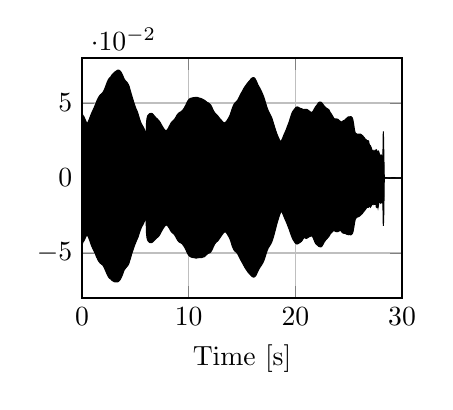
\begin{tikzpicture}

\begin{axis}[%
width=1.6in,
height=1.2in,
at={(0.758in,0.481in)},
scale only axis,
xmin=0,
xmax=30,
xmajorgrids,
ymin=-0.08,
ymax=0.08,
ymajorgrids,
xlabel={Time [s]},
axis background/.style={fill=white}
]
\addplot[fill=black,draw=black,forget plot] plot table[row sep=crcr]{%
2.08333333333333e-05	0.0536211729049683\\
0.0417454218822439	0.0417503118515015\\
0.0834700104311544	0.0416415929794312\\
0.125194598980065	0.0413455963134766\\
0.166919187528975	0.0409034490585327\\
0.208643776077886	0.0402671098709106\\
0.250368364626797	0.0396071672439575\\
0.292092953175707	0.0388947725296021\\
0.333817541724618	0.0382143259048462\\
0.375542130273528	0.0375051498413086\\
0.417266718822439	0.0369267463684082\\
0.458991307371349	0.0365341901779175\\
0.50071589592026	0.0366325378417969\\
0.54244048446917	0.036968469619751\\
0.584165073018081	0.0374776124954224\\
0.625889661566991	0.038111686706543\\
0.667614250115902	0.0387946367263794\\
0.709338838664812	0.0396475791931152\\
0.751063427213723	0.0403919219970703\\
0.792788015762633	0.0412305593490601\\
0.834512604311544	0.04195237159729\\
0.876237192860454	0.0427013635635376\\
0.917961781409365	0.0433881282806396\\
0.959686369958275	0.0441036224365234\\
1.00141095850719	0.0447241067886353\\
1.0431355470561	0.0453665256500244\\
1.08486013560501	0.045982837677002\\
1.12658472415392	0.046648383140564\\
1.16830931270283	0.0473350286483765\\
1.21003390125174	0.0481044054031372\\
1.25175848980065	0.0488525629043579\\
1.29348307834956	0.0495905876159668\\
1.33520766689847	0.0503195524215698\\
1.37693225544738	0.0510613918304443\\
1.41865684399629	0.051735520362854\\
1.4603814325452	0.0523669719696045\\
1.50210602109411	0.0530439615249634\\
1.54383060964302	0.053600549697876\\
1.58555519819193	0.0540659427642822\\
1.62727978674084	0.0545057058334351\\
1.66900437528975	0.0549044609069824\\
1.71072896383866	0.0553078651428223\\
1.75245355238758	0.0556150674819946\\
1.79417814093649	0.05585777759552\\
1.8359027294854	0.0560944080352783\\
1.87762731803431	0.0563201904296875\\
1.91935190658322	0.0566680431365967\\
1.96107649513213	0.0570636987686157\\
2.00280108368104	0.0575522184371948\\
2.04452567222995	0.0581012964248657\\
2.08625026077886	0.058653712272644\\
2.12797484932777	0.059423565864563\\
2.16969943787668	0.0601707696914673\\
2.21142402642559	0.0610047578811646\\
2.2531486149745	0.0617378950119019\\
2.29487320352341	0.062546968460083\\
2.33659779207232	0.0632725954055786\\
2.37832238062123	0.0640906095504761\\
2.42004696917014	0.0647281408309937\\
2.46177155771905	0.0653953552246094\\
2.50349614626796	0.0658761262893677\\
2.54522073481687	0.0662523508071899\\
2.58694532336579	0.0666037797927856\\
2.6286699119147	0.0669161081314087\\
2.67039450046361	0.067272424697876\\
2.71211908901252	0.0674711465835571\\
2.75384367756143	0.068170428276062\\
2.79556826611034	0.0685280561447144\\
2.83729285465925	0.0688735246658325\\
2.87901744320816	0.0692380666732788\\
2.92074203175707	0.0695731639862061\\
2.96246662030598	0.069798469543457\\
3.00419120885489	0.0701042413711548\\
3.0459157974038	0.0703350305557251\\
3.08764038595271	0.070637583732605\\
3.12936497450162	0.0708303451538086\\
3.17108956305053	0.071061372756958\\
3.21281415159944	0.0712687969207764\\
3.25453874014835	0.0714657306671143\\
3.29626332869726	0.0716756582260132\\
3.33798791724618	0.0718185901641846\\
3.37971250579509	0.0718762874603271\\
3.421437094344	0.0718759298324585\\
3.46316168289291	0.0718058347702026\\
3.50488627144182	0.0716338157653809\\
3.54661085999073	0.0714178085327148\\
3.58833544853964	0.0710142850875854\\
3.63006003708855	0.0707372426986694\\
3.67178462563746	0.0702794790267944\\
3.71350921418637	0.0697504281997681\\
3.75523380273528	0.0691699981689453\\
3.79695839128419	0.0684798955917358\\
3.8386829798331	0.0677869319915771\\
3.88040756838201	0.0670654773712158\\
3.92213215693092	0.0664634704589844\\
3.96385674547983	0.0657613277435303\\
4.00558133402874	0.0653648376464844\\
4.04730592257765	0.0649609565734863\\
4.08903051112656	0.064652681350708\\
4.13075509967547	0.0642834901809692\\
4.17247968822439	0.0640044212341309\\
4.2142042767733	0.0636613368988037\\
4.25592886532221	0.063287615776062\\
4.29765345387112	0.0627796649932861\\
4.33937804242003	0.0622220039367676\\
4.38110263096894	0.0615911483764648\\
4.42282721951785	0.0607218742370605\\
4.46455180806676	0.059624195098877\\
4.50627639661567	0.0585811138153076\\
4.54800098516458	0.0576307773590088\\
4.58972557371349	0.0564782619476318\\
4.6314501622624	0.0555140972137451\\
4.67317475081131	0.0545151233673096\\
4.71489933936022	0.0535752773284912\\
4.75662392790913	0.0525329113006592\\
4.79834851645804	0.0516151189804077\\
4.84007310500695	0.050533652305603\\
4.88179769355586	0.0496973991394043\\
4.92352228210478	0.0487895011901855\\
4.96524687065368	0.0479187965393066\\
5.0069714592026	0.0469344854354858\\
5.04869604775151	0.0462898015975952\\
5.09042063630042	0.0455863475799561\\
5.13214522484933	0.0449589490890503\\
5.17386981339824	0.0442054271697998\\
5.21559440194715	0.0433125495910645\\
5.25731899049606	0.0425401926040649\\
5.29904357904497	0.0414361953735352\\
5.34076816759388	0.0404845476150513\\
5.38249275614279	0.039512038230896\\
5.4242173446917	0.0386048555374146\\
5.46594193324061	0.0377095937728882\\
5.50766652178952	0.0369284152984619\\
5.54939111033843	0.0361937284469604\\
5.59111569888734	0.0356755256652832\\
5.63284028743625	0.0352612733840942\\
5.67456487598516	0.0346895456314087\\
5.71628946453407	0.0341701507568359\\
5.75801405308299	0.0336339473724365\\
5.7997386416319	0.0330507755279541\\
5.84146323018081	0.0324047803878784\\
5.88318781872972	0.0316872596740723\\
5.92491240727863	0.00985455513000488\\
5.96663699582754	0.00974833965301514\\
6.00836158437645	0.0274226665496826\\
6.05008617292536	0.0368496179580688\\
6.09181076147427	0.0396149158477783\\
6.13353535002318	0.040865421295166\\
6.17525993857209	0.0415663719177246\\
6.216984527121	0.0419789552688599\\
6.25870911566991	0.0422769784927368\\
6.30043370421882	0.0426157712936401\\
6.34215829276773	0.0428085327148438\\
6.38388288131664	0.0428472757339478\\
6.42560746986555	0.0429450273513794\\
6.46733205841446	0.042987585067749\\
6.50905664696338	0.0429986715316772\\
6.55078123551229	0.0429160594940186\\
6.5925058240612	0.0427892208099365\\
6.63423041261011	0.0424802303314209\\
6.67595500115902	0.0421701669692993\\
6.71767958970793	0.0418351888656616\\
6.75940417825684	0.0414478778839111\\
6.80112876680575	0.0411292314529419\\
6.84285335535466	0.0407865047454834\\
6.88457794390357	0.0403852462768555\\
6.92630253245248	0.0401281118392944\\
6.96802712100139	0.0397789478302002\\
7.0097517095503	0.039556622505188\\
7.05147629809921	0.0393797159194946\\
7.09320088664812	0.0390063524246216\\
7.13492547519703	0.0386742353439331\\
7.17665006374594	0.0383428335189819\\
7.21837465229485	0.037961483001709\\
7.26009924084376	0.0376327037811279\\
7.30182382939268	0.0371971130371094\\
7.34354841794159	0.0366947650909424\\
7.3852730064905	0.0360722541809082\\
7.42699759503941	0.0355774164199829\\
7.46872218358832	0.0351443290710449\\
7.51044677213723	0.0345486402511597\\
7.55217136068614	0.0340394973754883\\
7.59389594923505	0.0335434675216675\\
7.63562053778396	0.0330874919891357\\
7.67734512633287	0.032678484916687\\
7.71906971488178	0.0322834253311157\\
7.76079430343069	0.0320020914077759\\
7.8025188919796	0.0316950082778931\\
7.84424348052851	0.0315449237823486\\
7.88596806907742	0.0315548181533813\\
7.92769265762633	0.0316784381866455\\
7.96941724617524	0.0318373441696167\\
8.01114183472416	0.0322262048721313\\
8.05286642327307	0.0326384305953979\\
8.09459101182198	0.0331169366836548\\
8.13631560037089	0.0337187051773071\\
8.1780401889198	0.0343832969665527\\
8.21976477746871	0.0349199771881104\\
8.26148936601762	0.0355252027511597\\
8.30321395456653	0.0360413789749146\\
8.34493854311544	0.0365328788757324\\
8.38666313166435	0.0369856357574463\\
8.42838772021326	0.0373965501785278\\
8.47011230876217	0.0376728773117065\\
8.51183689731108	0.0379461050033569\\
8.55356148585999	0.0381652116775513\\
8.5952860744089	0.0384188890457153\\
8.63701066295781	0.0387550592422485\\
8.67873525150672	0.0391108989715576\\
8.72045984005563	0.0395323038101196\\
8.76218442860454	0.040026068687439\\
8.80390901715345	0.0405654907226563\\
8.84563360570237	0.041109561920166\\
8.88735819425128	0.0416519641876221\\
8.92908278280018	0.042056679725647\\
8.9708073713491	0.0424346923828125\\
9.01253195989801	0.0427476167678833\\
9.05425654844692	0.0430654287338257\\
9.09598113699583	0.0433433055877686\\
9.13770572554474	0.0435569286346436\\
9.17943031409365	0.0437279939651489\\
9.22115490264256	0.0439050197601318\\
9.26287949119147	0.0440822839736938\\
9.30460407974038	0.0442284345626831\\
9.34632866828929	0.0444490909576416\\
9.3880532568382	0.0447574853897095\\
9.42977784538711	0.0450403690338135\\
9.47150243393602	0.0453952550888062\\
9.51322702248493	0.0458188056945801\\
9.55495161103384	0.0462744235992432\\
9.59667619958275	0.0467684268951416\\
9.63840078813166	0.0473216772079468\\
9.68012537668058	0.0478912591934204\\
9.72184996522949	0.0483832359313965\\
9.7635745537784	0.049040675163269\\
9.80529914232731	0.0496599674224854\\
9.84702373087622	0.0503332614898682\\
9.88874831942513	0.0509045124053955\\
9.93047290797404	0.0514222383499146\\
9.97219749652295	0.0518299341201782\\
10.0139220850719	0.0521982908248901\\
10.0556466736208	0.0525182485580444\\
10.0973712621697	0.0527107715606689\\
10.1390958507186	0.0529539585113525\\
10.1808204392675	0.0529993772506714\\
10.2225450278164	0.0531057119369507\\
10.2642696163653	0.0531934499740601\\
10.3059942049142	0.0532735586166382\\
10.3477187934631	0.0533816814422607\\
10.3894433820121	0.0534257888793945\\
10.431167970561	0.0534718036651611\\
10.4728925591099	0.0535010099411011\\
10.5146171476588	0.0535497665405273\\
10.5563417362077	0.0535939931869507\\
10.5980663247566	0.053707480430603\\
10.6397909133055	0.0537416934967041\\
10.6815155018544	0.0537620782852173\\
10.7232400904033	0.0537128448486328\\
10.7649646789523	0.0536906719207764\\
10.8066892675012	0.0536403656005859\\
10.8484138560501	0.0535871982574463\\
10.890138444599	0.0534753799438477\\
10.9318630331479	0.0533620119094849\\
10.9735876216968	0.0532698631286621\\
11.0153122102457	0.0531817674636841\\
11.0570367987946	0.0531128644943237\\
11.0987613873435	0.0530664920806885\\
11.1404859758924	0.0529501438140869\\
11.1822105644414	0.0528137683868408\\
11.2239351529903	0.0526802539825439\\
11.2656597415392	0.0525555610656738\\
11.3073843300881	0.0524437427520752\\
11.349108918637	0.0522584915161133\\
11.3908335071859	0.0521126985549927\\
11.4325580957348	0.0519522428512573\\
11.4742826842837	0.0517711639404297\\
11.5160072728326	0.0515637397766113\\
11.5577318613816	0.0513095855712891\\
11.5994564499305	0.0510501861572266\\
11.6411810384794	0.0508202314376831\\
11.6829056270283	0.0505682229995728\\
11.7246302155772	0.0503746271133423\\
11.7663548041261	0.0502249002456665\\
11.808079392675	0.0500696897506714\\
11.8498039812239	0.049943208694458\\
11.8915285697728	0.0496844053268433\\
11.9332531583217	0.0495097637176514\\
11.9749777468707	0.0492569208145142\\
12.0167023354196	0.0489706993103027\\
12.0584269239685	0.0485762357711792\\
12.1001515125174	0.0481170415878296\\
12.1418761010663	0.0475074052810669\\
12.1836006896152	0.0468636751174927\\
12.2253252781641	0.0461859703063965\\
12.267049866713	0.0455539226531982\\
12.3087744552619	0.0449726581573486\\
12.3504990438108	0.0444214344024658\\
12.3922236323598	0.043917179107666\\
12.4339482209087	0.0434936285018921\\
12.4756728094576	0.0431104898452759\\
12.5173973980065	0.0427876710891724\\
12.5591219865554	0.0425126552581787\\
12.6008465751043	0.0422230958938599\\
12.6425711636532	0.0418906211853027\\
12.6842957522021	0.0415650606155396\\
12.726020340751	0.0412672758102417\\
12.7677449293	0.0409246683120728\\
12.8094695178489	0.0405149459838867\\
12.8511941063978	0.040174126625061\\
12.8929186949467	0.0397669076919556\\
12.9346432834956	0.0393375158309937\\
12.9763678720445	0.0390839576721191\\
13.0180924605934	0.0387721061706543\\
13.0598170491423	0.0384184122085571\\
13.1015416376912	0.038081169128418\\
13.1432662262401	0.0376831293106079\\
13.1849908147891	0.0373498201370239\\
13.226715403338	0.0371320247650146\\
13.2684399918869	0.0368905067443848\\
13.3101645804358	0.036737322807312\\
13.3518891689847	0.0366839170455933\\
13.3936137575336	0.0367783308029175\\
13.4353383460825	0.0369142293930054\\
13.4770629346314	0.0372158288955688\\
13.5187875231803	0.0374529361724854\\
13.5605121117293	0.037878155708313\\
13.6022367002782	0.0383341312408447\\
13.6439612888271	0.0387896299362183\\
13.685685877376	0.0392775535583496\\
13.7274104659249	0.0397576093673706\\
13.7691350544738	0.0402729511260986\\
13.8108596430227	0.0407878160476685\\
13.8525842315716	0.0414515733718872\\
13.8943088201205	0.0421701669692993\\
13.9360334086694	0.0431364774703979\\
13.9777579972184	0.0440064668655396\\
14.0194825857673	0.0449142456054688\\
14.0612071743162	0.0458117723464966\\
14.1029317628651	0.0466654300689697\\
14.144656351414	0.0474077463150024\\
14.1863809399629	0.0480997562408447\\
14.2281055285118	0.0487645864486694\\
14.2698301170607	0.0492068529129028\\
14.3115547056096	0.0496878623962402\\
14.3532792941586	0.0500575304031372\\
14.3950038827075	0.0503883361816406\\
14.4367284712564	0.0506373643875122\\
14.4784530598053	0.0509068965911865\\
14.5201776483542	0.0512329339981079\\
14.5619022369031	0.0515708923339844\\
14.603626825452	0.0520197153091431\\
14.6453514140009	0.0525741577148438\\
14.6870760025498	0.0531100034713745\\
14.7288005910988	0.0536602735519409\\
14.7705251796477	0.0542706251144409\\
14.8122497681966	0.0548862218856812\\
14.8539743567455	0.0554665327072144\\
14.8956989452944	0.0560730695724487\\
14.9374235338433	0.056658148765564\\
14.9791481223922	0.0571459531784058\\
15.0208727109411	0.0576331615447998\\
15.06259729949	0.0582407712936401\\
15.1043218880389	0.0587902069091797\\
15.1460464765879	0.059303879737854\\
15.1877710651368	0.0598244667053223\\
15.2294956536857	0.0603344440460205\\
15.2712202422346	0.0608099699020386\\
15.3129448307835	0.0611622333526611\\
15.3546694193324	0.0616819858551025\\
15.3963940078813	0.0619277954101563\\
15.4381185964302	0.0624451637268066\\
15.4798431849791	0.0628286600112915\\
15.521567773528	0.063166618347168\\
15.563292362077	0.0635663270950317\\
15.6050169506259	0.0639395713806152\\
15.6467415391748	0.0643100738525391\\
15.6884661277237	0.0646368265151978\\
15.7301907162726	0.0649843215942383\\
15.7719153048215	0.065266489982605\\
15.8136398933704	0.0657442808151245\\
15.8553644819193	0.0660792589187622\\
15.8970890704682	0.0663728713989258\\
15.9388136590172	0.066550612449646\\
15.9805382475661	0.0667105913162231\\
16.022262836115	0.0667927265167236\\
16.0639874246639	0.0668336153030396\\
16.1057120132128	0.0667902231216431\\
16.1474366017617	0.0666788816452026\\
16.1891611903106	0.0663776397705078\\
16.2308857788595	0.0659853219985962\\
16.2726103674084	0.0654909610748291\\
16.3143349559573	0.0649021863937378\\
16.3560595445063	0.0642683506011963\\
16.3977841330552	0.0635666847229004\\
16.4395087216041	0.0628879070281982\\
16.481233310153	0.062137246131897\\
16.5229578987019	0.0616699457168579\\
16.5646824872508	0.0610781908035278\\
16.6064070757997	0.0605579614639282\\
16.6481316643486	0.0599993467330933\\
16.6898562528975	0.0594977140426636\\
16.7315808414465	0.0588716268539429\\
16.7733054299954	0.0583078861236572\\
16.8150300185443	0.0576440095901489\\
16.8567546070932	0.0570241212844849\\
16.8984791956421	0.0563548803329468\\
16.940203784191	0.0556117296218872\\
16.9819283727399	0.0549261569976807\\
17.0236529612888	0.054167628288269\\
17.0653775498377	0.0532543659210205\\
17.1071021383867	0.0523369312286377\\
17.1488267269356	0.0513863563537598\\
17.1905513154845	0.0503770112991333\\
17.2322759040334	0.0493361949920654\\
17.2740004925823	0.0483777523040771\\
17.3157250811312	0.0474597215652466\\
17.3574496696801	0.0466158390045166\\
17.399174258229	0.0458483695983887\\
17.4408988467779	0.0450590848922729\\
17.4826234353268	0.0443686246871948\\
17.5243480238758	0.0437277555465698\\
17.5660726124247	0.0431736707687378\\
17.6077972009736	0.0425887107849121\\
17.6495217895225	0.0419580936431885\\
17.6912463780714	0.0413664579391479\\
17.7329709666203	0.040794849395752\\
17.7746955551692	0.0401002168655396\\
17.8164201437181	0.0393403768539429\\
17.858144732267	0.0384116172790527\\
17.8998693208159	0.037395715713501\\
17.9415939093649	0.0364679098129272\\
17.9833184979138	0.0355391502380371\\
18.0250430864627	0.0345214605331421\\
18.0667676750116	0.0335776805877686\\
18.1084922635605	0.0326200723648071\\
18.1502168521094	0.0316839218139648\\
18.1919414406583	0.0308010578155518\\
18.2336660292072	0.029976487159729\\
18.2753906177561	0.0291763544082642\\
18.3171152063051	0.0283764600753784\\
18.358839794854	0.0277289152145386\\
18.4005643834029	0.02704918384552\\
18.4422889719518	0.026366114616394\\
18.4840135605007	0.0256907939910889\\
18.5257381490496	0.0250957012176514\\
18.5674627375985	0.0246304273605347\\
18.6091873261474	0.0243680477142334\\
18.6509119146963	0.024425745010376\\
18.6926365032453	0.0247962474822998\\
18.7343610917942	0.0253227949142456\\
18.7760856803431	0.0259628295898438\\
18.817810268892	0.0266454219818115\\
18.8595348574409	0.027456521987915\\
18.9012594459898	0.0281568765640259\\
18.9429840345387	0.0289063453674316\\
18.9847086230876	0.0296013355255127\\
19.0264332116365	0.0302489995956421\\
19.0681578001854	0.0308760404586792\\
19.1098823887344	0.0315674543380737\\
19.1516069772833	0.0323046445846558\\
19.1933315658322	0.0331307649612427\\
19.2350561543811	0.0339244604110718\\
19.27678074293	0.0347599983215332\\
19.3185053314789	0.0354475975036621\\
19.3602299200278	0.0362244844436646\\
19.4019545085767	0.0370532274246216\\
19.4436790971256	0.037988543510437\\
19.4854036856745	0.0389022827148438\\
19.5271282742235	0.0398720502853394\\
19.5688528627724	0.0407732725143433\\
19.6105774513213	0.0417658090591431\\
19.6523020398702	0.0425513982772827\\
19.6940266284191	0.0433449745178223\\
19.735751216968	0.043904185295105\\
19.7774758055169	0.0444862842559814\\
19.8192003940658	0.044885516166687\\
19.8609249826147	0.0452675819396973\\
19.9026495711637	0.0456660985946655\\
19.9443741597126	0.0460711717605591\\
19.9860987482615	0.0464241504669189\\
20.0278233368104	0.0467612743377686\\
20.0695479253593	0.0470316410064697\\
20.1112725139082	0.0472245216369629\\
20.1529971024571	0.0472662448883057\\
20.194721691006	0.0472837686538696\\
20.2364462795549	0.0471764802932739\\
20.2781708681038	0.0470463037490845\\
20.3198954566528	0.0469015836715698\\
20.3616200452017	0.046721339225769\\
20.4033446337506	0.0465607643127441\\
20.4450692222995	0.0464258193969727\\
20.4867938108484	0.0463229417800903\\
20.5285183993973	0.0462146997451782\\
20.5702429879462	0.0461443662643433\\
20.6119675764951	0.0460717678070068\\
20.653692165044	0.0459364652633667\\
20.695416753593	0.0458433628082275\\
20.7371413421419	0.0456039905548096\\
20.7788659306908	0.0455809831619263\\
20.8205905192397	0.0456002950668335\\
20.8623151077886	0.045655369758606\\
20.9040396963375	0.0456995964050293\\
20.9457642848864	0.0457216501235962\\
20.9874888734353	0.0457353591918945\\
21.0292134619842	0.0456912517547607\\
21.0709380505331	0.0456423759460449\\
21.1126626390821	0.0455175638198853\\
21.154387227631	0.0453486442565918\\
21.1961118161799	0.0451440811157227\\
21.2378364047288	0.0448935031890869\\
21.2795609932777	0.0447086095809937\\
21.3212855818266	0.0444554090499878\\
21.3630101703755	0.0442345142364502\\
21.4047347589244	0.0440176725387573\\
21.4464593474733	0.043850302696228\\
21.4881839360223	0.0437244176864624\\
21.5299085245712	0.043750524520874\\
21.5716331131201	0.0438804626464844\\
21.613357701669	0.0441498756408691\\
21.6550822902179	0.0444552898406982\\
21.6968068787668	0.0449012517929077\\
21.7385314673157	0.0453757047653198\\
21.7802560558646	0.045989990234375\\
21.8219806444135	0.0465331077575684\\
21.8637052329624	0.0470596551895142\\
21.9054298215114	0.0475136041641235\\
21.9471544100603	0.0478919744491577\\
21.9888789986092	0.0481795072555542\\
22.0306035871581	0.04860520362854\\
22.072328175707	0.0490416288375854\\
22.1140527642559	0.0495084524154663\\
22.1557773528048	0.0500413179397583\\
22.1975019413537	0.0503033399581909\\
22.2392265299026	0.0504610538482666\\
22.2809511184516	0.0505561828613281\\
22.3226757070005	0.0505572557449341\\
22.3644002955494	0.0505557060241699\\
22.4061248840983	0.0504575967788696\\
22.4478494726472	0.0502573251724243\\
22.4895740611961	0.0498881340026855\\
22.531298649745	0.0495618581771851\\
22.5730232382939	0.0491092205047607\\
22.6147478268428	0.0487831830978394\\
22.6564724153917	0.0483672618865967\\
22.6981970039407	0.0479003190994263\\
22.7399215924896	0.0475746393203735\\
22.7816461810385	0.0473968982696533\\
22.8233707695874	0.0470458269119263\\
22.8650953581363	0.0467692613601685\\
22.9068199466852	0.0465277433395386\\
22.9485445352341	0.0462939739227295\\
22.990269123783	0.0461512804031372\\
23.0319937123319	0.0459285974502563\\
23.0737183008809	0.0458322763442993\\
23.1154428894298	0.0456206798553467\\
23.1571674779787	0.0451951026916504\\
23.1988920665276	0.0445874929428101\\
23.2406166550765	0.0439237356185913\\
23.2823412436254	0.0434198379516602\\
23.3240658321743	0.0430817604064941\\
23.3657904207232	0.0426479578018188\\
23.4075150092721	0.0421072244644165\\
23.449239597821	0.0416498184204102\\
23.49096418637	0.0411646366119385\\
23.5326887749189	0.0406177043914795\\
23.5744133634678	0.040058970451355\\
23.6161379520167	0.0396404266357422\\
23.6578625405656	0.0393742322921753\\
23.6995871291145	0.0393000841140747\\
23.7413117176634	0.0392686128616333\\
23.7830363062123	0.0392775535583496\\
23.8247608947612	0.0393209457397461\\
23.8664854833102	0.0392382144927979\\
23.9082100718591	0.0391891002655029\\
23.949934660408	0.0391485691070557\\
23.9916592489569	0.0390416383743286\\
24.0333838375058	0.0388131141662598\\
24.0751084260547	0.0385217666625977\\
24.1168330146036	0.0381946563720703\\
24.1585576031525	0.0380316972732544\\
24.2002821917014	0.0377241373062134\\
24.2420067802503	0.0374670028686523\\
24.2837313687993	0.0372993946075439\\
24.3254559573482	0.0372902154922485\\
24.3671805458971	0.0374517440795898\\
24.408905134446	0.0376710891723633\\
24.4506297229949	0.0378634929656982\\
24.4923543115438	0.0380678176879883\\
24.5340789000927	0.0382248163223267\\
24.5758034886416	0.0383361577987671\\
24.6175280771905	0.0385164022445679\\
24.6592526657395	0.0387388467788696\\
24.7009772542884	0.0390697717666626\\
24.7427018428373	0.0393558740615845\\
24.7844264313862	0.0396963357925415\\
24.8261510199351	0.0398381948471069\\
24.867875608484	0.040074348449707\\
24.9096001970329	0.0402921438217163\\
24.9513247855818	0.0406334400177002\\
24.9930493741307	0.0406596660614014\\
25.0347739626796	0.0405958890914917\\
25.0764985512286	0.0406510829925537\\
25.1182231397775	0.0407745838165283\\
25.1599477283264	0.0408613681793213\\
25.2016723168753	0.0408817529678345\\
25.2433969054242	0.0406763553619385\\
25.2851214939731	0.0403909683227539\\
25.326846082522	0.0401537418365479\\
25.3685706710709	0.0393996238708496\\
25.4102952596198	0.0380069017410278\\
25.4520198481687	0.0362684726715088\\
25.4937444367177	0.0342063903808594\\
25.5354690252666	0.0322630405426025\\
25.5771936138155	0.0307275056838989\\
25.6189182023644	0.0300391912460327\\
25.6606427909133	0.0296636819839478\\
25.7023673794622	0.0295193195343018\\
25.7440919680111	0.0292972326278687\\
25.78581655656	0.0291728973388672\\
25.8275411451089	0.0291287899017334\\
25.8692657336579	0.0291379690170288\\
25.9109903222068	0.0291287899017334\\
25.9527149107557	0.0291281938552856\\
25.9944394993046	0.0291746854782104\\
26.0361640878535	0.0291982889175415\\
26.0778886764024	0.0292426347732544\\
26.1196132649513	0.0291390419006348\\
26.1613378535002	0.028888463973999\\
26.2030624420491	0.0286865234375\\
26.2447870305981	0.0284223556518555\\
26.286511619147	0.0282833576202393\\
26.3282362076959	0.0279566049575806\\
26.3699607962448	0.0275673866271973\\
26.4116853847937	0.0272645950317383\\
26.4534099733426	0.0269160270690918\\
26.4951345618915	0.026465892791748\\
26.5368591504404	0.0260282754898071\\
26.5785837389893	0.0257561206817627\\
26.6203083275383	0.0255717039108276\\
26.6620329160872	0.0252395868301392\\
26.7037575046361	0.0249288082122803\\
26.745482093185	0.0248153209686279\\
26.7872066817339	0.0248095989227295\\
26.8289312702828	0.0247689485549927\\
26.8706558588317	0.0243176221847534\\
26.9123804473806	0.0225847959518433\\
26.9541050359295	0.0219802856445313\\
26.9958296244784	0.0216488838195801\\
27.0375542130274	0.0213974714279175\\
27.0792788015763	0.0206676721572876\\
27.1210033901252	0.0198719501495361\\
27.1627279786741	0.0188684463500977\\
27.204452567223	0.0181429386138916\\
27.2461771557719	0.0178501605987549\\
27.2879017443208	0.018254280090332\\
27.3296263328697	0.0177537202835083\\
27.3713509214186	0.0167869329452515\\
27.4130755099675	0.0176242589950562\\
27.4548000985165	0.0181742906570435\\
27.4965246870654	0.0177152156829834\\
27.5382492756143	0.0170744657516479\\
27.5799738641632	0.0187968015670776\\
27.6216984527121	0.0185747146606445\\
27.663423041261	0.017472505569458\\
27.7051476298099	0.0164626836776733\\
27.7468722183588	0.0168507099151611\\
27.7885968069077	0.0177123546600342\\
27.8303213954567	0.0172004699707031\\
27.8720459840056	0.0159845352172852\\
27.9137705725545	0.0147225856781006\\
27.9554951611034	0.0139701366424561\\
27.9972197496523	0.0147663354873657\\
28.0389443382012	0.0152850151062012\\
28.0806689267501	0.0148869752883911\\
28.122393515299	0.0144383907318115\\
28.1641181038479	0.0146770477294922\\
28.2058426923968	0.012948751449585\\
28.2475672809458	0.0309923887252808\\
28.2892918694947	0.0158401727676392\\
28.3310164580436	0.000872492790222168\\
28.3727410465925	0.000297904014587402\\
28.4144656351414	0.000198245048522949\\
28.4561902236903	0.000166893005371094\\
28.4979148122392	0.000153899192810059\\
28.5396394007881	0.000149011611938477\\
28.581363989337	0.000105977058410645\\
28.623088577886	7.00950622558594e-05\\
28.6648131664349	4.97102737426758e-05\\
28.7065377549838	1.54972076416016e-05\\
28.7482623435327	1.33514404296875e-05\\
28.7899869320816	3.814697265625e-06\\
28.8317115206305	3.33786010742188e-06\\
28.8734361091794	2.55107879638672e-05\\
28.9151606977283	2.59876251220703e-05\\
28.9568852862772	7.84397125244141e-05\\
28.9986098748261	8.72611999511719e-05\\
29.0403344633751	0.000134706497192383\\
29.082059051924	0.000158548355102539\\
29.1237836404729	0.000167727470397949\\
29.1655082290218	0.000154852867126465\\
29.2072328175707	0.000173687934875488\\
29.2489574061196	0.000199079513549805\\
29.2906819946685	0.000167250633239746\\
29.3324065832174	0.000147700309753418\\
29.3741311717663	0.000101923942565918\\
29.4158557603153	8.17775726318359e-05\\
29.4575803488642	8.55922698974609e-05\\
29.4993049374131	7.27176666259766e-05\\
29.541029525962	8.17775726318359e-05\\
29.5827541145109	7.39097595214844e-05\\
29.6244787030598	6.54458999633789e-05\\
29.6662032916087	4.29153442382813e-05\\
29.7079278801576	4.05311584472656e-05\\
29.7496524687065	4.38690185546875e-05\\
29.7913770572554	4.80413436889648e-05\\
29.8331016458044	5.38825988769531e-05\\
29.8748262343533	4.67300415039063e-05\\
29.9165508229022	3.96966934204102e-05\\
29.9582754114511	4.01735305786133e-05\\
30	6.09159469604492e-05\\
}
\closedcycle;
\addplot[fill=black,draw=black,forget plot] plot table[row sep=crcr]{%
2.08333333333333e-05	-0.0558394193649292\\
0.0417454218822439	-0.0428831577301025\\
0.0834700104311544	-0.0427399873733521\\
0.125194598980065	-0.0424689054489136\\
0.166919187528975	-0.0420178174972534\\
0.208643776077886	-0.0414783954620361\\
0.250368364626797	-0.0408487319946289\\
0.292092953175707	-0.0401557683944702\\
0.333817541724618	-0.0394546985626221\\
0.375542130273528	-0.0388714075088501\\
0.417266718822439	-0.0384417772293091\\
0.458991307371349	-0.0381721258163452\\
0.50071589592026	-0.0382364988327026\\
0.54244048446917	-0.0385943651199341\\
0.584165073018081	-0.0391639471054077\\
0.625889661566991	-0.0398472547531128\\
0.667614250115902	-0.0406070947647095\\
0.709338838664812	-0.0414090156555176\\
0.751063427213723	-0.0422514677047729\\
0.792788015762633	-0.0430949926376343\\
0.834512604311544	-0.0439167022705078\\
0.876237192860454	-0.0447962284088135\\
0.917961781409365	-0.0455245971679688\\
0.959686369958275	-0.0462243556976318\\
1.00141095850719	-0.0468647480010986\\
1.0431355470561	-0.0474865436553955\\
1.08486013560501	-0.0481202602386475\\
1.12658472415392	-0.0487635135650635\\
1.16830931270283	-0.0493468046188354\\
1.21003390125174	-0.0500298738479614\\
1.25175848980065	-0.0506800413131714\\
1.29348307834956	-0.0513826608657837\\
1.33520766689847	-0.0521631240844727\\
1.37693225544738	-0.052854061126709\\
1.41865684399629	-0.0534054040908813\\
1.4603814325452	-0.0540424585342407\\
1.50210602109411	-0.0546537637710571\\
1.54383060964302	-0.0551621913909912\\
1.58555519819193	-0.0556659698486328\\
1.62727978674084	-0.0560731887817383\\
1.66900437528975	-0.0563994646072388\\
1.71072896383866	-0.0567390918731689\\
1.75245355238758	-0.0569876432418823\\
1.79417814093649	-0.0572918653488159\\
1.8359027294854	-0.0575146675109863\\
1.87762731803431	-0.0577002763748169\\
1.91935190658322	-0.0579226016998291\\
1.96107649513213	-0.0582782030105591\\
2.00280108368104	-0.0587069988250732\\
2.04452567222995	-0.0592716932296753\\
2.08625026077886	-0.0598974227905273\\
2.12797484932777	-0.0605041980743408\\
2.16969943787668	-0.0611299276351929\\
2.21142402642559	-0.0617954730987549\\
2.2531486149745	-0.0625209808349609\\
2.29487320352341	-0.0632182359695435\\
2.33659779207232	-0.0639073848724365\\
2.37832238062123	-0.064558744430542\\
2.42004696917014	-0.0651462078094482\\
2.46177155771905	-0.0656810998916626\\
2.50349614626796	-0.0661267042160034\\
2.54522073481687	-0.0665807723999023\\
2.58694532336579	-0.0668585300445557\\
2.6286699119147	-0.0670897960662842\\
2.67039450046361	-0.0672465562820435\\
2.71211908901252	-0.0674610137939453\\
2.75384367756143	-0.0678273439407349\\
2.79556826611034	-0.0681569576263428\\
2.83729285465925	-0.0683680772781372\\
2.87901744320816	-0.0685478448867798\\
2.92074203175707	-0.0687289237976074\\
2.96246662030598	-0.0688533782958984\\
3.00419120885489	-0.0690850019454956\\
3.0459157974038	-0.069186806678772\\
3.08764038595271	-0.0692868232727051\\
3.12936497450162	-0.0692739486694336\\
3.17108956305053	-0.0692288875579834\\
3.21281415159944	-0.0692437887191772\\
3.25453874014835	-0.0692601203918457\\
3.29626332869726	-0.0692905187606812\\
3.33798791724618	-0.0692050457000732\\
3.37971250579509	-0.0691083669662476\\
3.421437094344	-0.0689351558685303\\
3.46316168289291	-0.0686897039413452\\
3.50488627144182	-0.0683751106262207\\
3.54661085999073	-0.0680162906646729\\
3.58833544853964	-0.0674960613250732\\
3.63006003708855	-0.0669950246810913\\
3.67178462563746	-0.0663665533065796\\
3.71350921418637	-0.0657140016555786\\
3.75523380273528	-0.0650453567504883\\
3.79695839128419	-0.0642943382263184\\
3.8386829798331	-0.063503623008728\\
3.88040756838201	-0.0626094341278076\\
3.92213215693092	-0.0617125034332275\\
3.96385674547983	-0.0612542629241943\\
4.00558133402874	-0.060752272605896\\
4.04730592257765	-0.0604143142700195\\
4.08903051112656	-0.0600622892379761\\
4.13075509967547	-0.0596408843994141\\
4.17247968822439	-0.0593078136444092\\
4.2142042767733	-0.0590062141418457\\
4.25592886532221	-0.0586198568344116\\
4.29765345387112	-0.0581976175308228\\
4.33937804242003	-0.0576620101928711\\
4.38110263096894	-0.0570361614227295\\
4.42282721951785	-0.0561273097991943\\
4.46455180806676	-0.0551731586456299\\
4.50627639661567	-0.0541908740997314\\
4.54800098516458	-0.0533030033111572\\
4.58972557371349	-0.0522016286849976\\
4.6314501622624	-0.0511406660079956\\
4.67317475081131	-0.0502121448516846\\
4.71489933936022	-0.0493117570877075\\
4.75662392790913	-0.0484828948974609\\
4.79834851645804	-0.0475808382034302\\
4.84007310500695	-0.0465869903564453\\
4.88179769355586	-0.0457291603088379\\
4.92352228210478	-0.0449137687683105\\
4.96524687065368	-0.0441511869430542\\
5.0069714592026	-0.0434781312942505\\
5.04869604775151	-0.0426920652389526\\
5.09042063630042	-0.0419275760650635\\
5.13214522484933	-0.0413268804550171\\
5.17386981339824	-0.0406374931335449\\
5.21559440194715	-0.0398952960968018\\
5.25731899049606	-0.0392297506332397\\
5.29904357904497	-0.0382956266403198\\
5.34076816759388	-0.0372313261032104\\
5.38249275614279	-0.0363105535507202\\
5.4242173446917	-0.0354714393615723\\
5.46594193324061	-0.0346640348434448\\
5.50766652178952	-0.0339368581771851\\
5.54939111033843	-0.0331436395645142\\
5.59111569888734	-0.032530665397644\\
5.63284028743625	-0.031994104385376\\
5.67456487598516	-0.0314675569534302\\
5.71628946453407	-0.0309311151504517\\
5.75801405308299	-0.0303608179092407\\
5.7997386416319	-0.0296889543533325\\
5.84146323018081	-0.0290205478668213\\
5.88318781872972	-0.02829909324646\\
5.92491240727863	-0.00833594799041748\\
5.96663699582754	-0.00832080841064453\\
6.00836158437645	-0.0283833742141724\\
6.05008617292536	-0.0372070074081421\\
6.09181076147427	-0.0398319959640503\\
6.13353535002318	-0.0410811901092529\\
6.17525993857209	-0.0417364835739136\\
6.216984527121	-0.0421900749206543\\
6.25870911566991	-0.0424246788024902\\
6.30043370421882	-0.0427963733673096\\
6.34215829276773	-0.0429587364196777\\
6.38388288131664	-0.0431039333343506\\
6.42560746986555	-0.0431439876556396\\
6.46733205841446	-0.0431418418884277\\
6.50905664696338	-0.0430954694747925\\
6.55078123551229	-0.0429614782333374\\
6.5925058240612	-0.0428346395492554\\
6.63423041261011	-0.0426064729690552\\
6.67595500115902	-0.0423203706741333\\
6.71767958970793	-0.0419782400131226\\
6.75940417825684	-0.0416585206985474\\
6.80112876680575	-0.041323184967041\\
6.84285335535466	-0.0410563945770264\\
6.88457794390357	-0.0407577753067017\\
6.92630253245248	-0.0404735803604126\\
6.96802712100139	-0.0401731729507446\\
7.0097517095503	-0.0399316549301147\\
7.05147629809921	-0.039671778678894\\
7.09320088664812	-0.0394405126571655\\
7.13492547519703	-0.0392115116119385\\
7.17665006374594	-0.0388325452804565\\
7.21837465229485	-0.0384591817855835\\
7.26009924084376	-0.0380232334136963\\
7.30182382939268	-0.0376038551330566\\
7.34354841794159	-0.0370043516159058\\
7.3852730064905	-0.0363801717758179\\
7.42699759503941	-0.0358481407165527\\
7.46872218358832	-0.035256028175354\\
7.51044677213723	-0.0347692966461182\\
7.55217136068614	-0.0342142581939697\\
7.59389594923505	-0.0337228775024414\\
7.63562053778396	-0.0332998037338257\\
7.67734512633287	-0.0328482389450073\\
7.71906971488178	-0.0324126482009888\\
7.76079430343069	-0.0320326089859009\\
7.8025188919796	-0.031735897064209\\
7.84424348052851	-0.0315624475479126\\
7.88596806907742	-0.0314326286315918\\
7.92769265762633	-0.0313937664031982\\
7.96941724617524	-0.031537652015686\\
8.01114183472416	-0.0317338705062866\\
8.05286642327307	-0.0320823192596436\\
8.09459101182198	-0.0325053930282593\\
8.13631560037089	-0.0329684019088745\\
8.1780401889198	-0.033394455909729\\
8.21976477746871	-0.0339415073394775\\
8.26148936601762	-0.0345425605773926\\
8.30321395456653	-0.0350098609924316\\
8.34493854311544	-0.0355530977249146\\
8.38666313166435	-0.0358841419219971\\
8.42838772021326	-0.0362515449523926\\
8.47011230876217	-0.0364927053451538\\
8.51183689731108	-0.0367769002914429\\
8.55356148585999	-0.0369881391525269\\
8.5952860744089	-0.0372492074966431\\
8.63701066295781	-0.0375308990478516\\
8.67873525150672	-0.0379055738449097\\
8.72045984005563	-0.0383578538894653\\
8.76218442860454	-0.0388818979263306\\
8.80390901715345	-0.0394589900970459\\
8.84563360570237	-0.0400673151016235\\
8.88735819425128	-0.0405832529067993\\
8.92908278280018	-0.0410678386688232\\
8.9708073713491	-0.0415141582489014\\
9.01253195989801	-0.0419367551803589\\
9.05425654844692	-0.042272686958313\\
9.09598113699583	-0.0425732135772705\\
9.13770572554474	-0.0427829027175903\\
9.17943031409365	-0.0429545640945435\\
9.22115490264256	-0.0431381464004517\\
9.26287949119147	-0.043304443359375\\
9.30460407974038	-0.0434726476669312\\
9.34632866828929	-0.0436323881149292\\
9.3880532568382	-0.04384446144104\\
9.42977784538711	-0.0442296266555786\\
9.47150243393602	-0.0445886850357056\\
9.51322702248493	-0.0450536012649536\\
9.55495161103384	-0.0454820394515991\\
9.59667619958275	-0.0459252595901489\\
9.63840078813166	-0.0464403629302979\\
9.68012537668058	-0.0470033884048462\\
9.72184996522949	-0.0476529598236084\\
9.7635745537784	-0.0482616424560547\\
9.80529914232731	-0.0489041805267334\\
9.84702373087622	-0.0495054721832275\\
9.88874831942513	-0.0501362085342407\\
9.93047290797404	-0.0506916046142578\\
9.97219749652295	-0.0511101484298706\\
10.0139220850719	-0.0515849590301514\\
10.0556466736208	-0.0518686771392822\\
10.0973712621697	-0.0521914958953857\\
10.1390958507186	-0.0523681640625\\
10.1808204392675	-0.0525816679000854\\
10.2225450278164	-0.0527130365371704\\
10.2642696163653	-0.0528024435043335\\
10.3059942049142	-0.0528905391693115\\
10.3477187934631	-0.0529372692108154\\
10.3894433820121	-0.0530189275741577\\
10.431167970561	-0.0530719757080078\\
10.4728925591099	-0.0531467199325562\\
10.5146171476588	-0.0531507730484009\\
10.5563417362077	-0.0531888008117676\\
10.5980663247566	-0.0532388687133789\\
10.6397909133055	-0.0533301830291748\\
10.6815155018544	-0.0533844232559204\\
10.7232400904033	-0.0533581972122192\\
10.7649646789523	-0.0533181428909302\\
10.8066892675012	-0.0533088445663452\\
10.8484138560501	-0.053205132484436\\
10.890138444599	-0.0531692504882813\\
10.9318630331479	-0.0531387329101563\\
10.9735876216968	-0.0531494617462158\\
11.0153122102457	-0.0531537532806396\\
11.0570367987946	-0.0531378984451294\\
11.0987613873435	-0.0531362295150757\\
11.1404859758924	-0.053144097328186\\
11.1822105644414	-0.0531095266342163\\
11.2239351529903	-0.053038477897644\\
11.2656597415392	-0.052959680557251\\
11.3073843300881	-0.0527887344360352\\
11.349108918637	-0.0527311563491821\\
11.3908335071859	-0.0526138544082642\\
11.4325580957348	-0.05255126953125\\
11.4742826842837	-0.0524276494979858\\
11.5160072728326	-0.0522420406341553\\
11.5577318613816	-0.0519609451293945\\
11.5994564499305	-0.0516455173492432\\
11.6411810384794	-0.0513311624526978\\
11.6829056270283	-0.0511026382446289\\
11.7246302155772	-0.0507820844650269\\
11.7663548041261	-0.0504680871963501\\
11.808079392675	-0.0502831935882568\\
11.8498039812239	-0.0501570701599121\\
11.8915285697728	-0.0500727891921997\\
11.9332531583217	-0.0499964952468872\\
11.9749777468707	-0.0498825311660767\\
12.0167023354196	-0.0496081113815308\\
12.0584269239685	-0.0492864847183228\\
12.1001515125174	-0.0488979816436768\\
12.1418761010663	-0.0484527349472046\\
12.1836006896152	-0.047899603843689\\
12.2253252781641	-0.0472328662872314\\
12.267049866713	-0.0465292930603027\\
12.3087744552619	-0.0458576679229736\\
12.3504990438108	-0.0452525615692139\\
12.3922236323598	-0.044668436050415\\
12.4339482209087	-0.0440919399261475\\
12.4756728094576	-0.0437189340591431\\
12.5173973980065	-0.0432753562927246\\
12.5591219865554	-0.042946457862854\\
12.6008465751043	-0.0426466464996338\\
12.6425711636532	-0.0424137115478516\\
12.6842957522021	-0.04218590259552\\
12.726020340751	-0.041862964630127\\
12.7677449293	-0.0415170192718506\\
12.8094695178489	-0.041093111038208\\
12.8511941063978	-0.0406923294067383\\
12.8929186949467	-0.0402761697769165\\
12.9346432834956	-0.0398080348968506\\
12.9763678720445	-0.0393524169921875\\
13.0180924605934	-0.0388872623443604\\
13.0598170491423	-0.0384643077850342\\
13.1015416376912	-0.0380803346633911\\
13.1432662262401	-0.0376843214035034\\
13.1849908147891	-0.0372864007949829\\
13.226715403338	-0.0369205474853516\\
13.2684399918869	-0.0365757942199707\\
13.3101645804358	-0.0362483263015747\\
13.3518891689847	-0.0360804796218872\\
13.3936137575336	-0.0359636545181274\\
13.4353383460825	-0.0359300374984741\\
13.4770629346314	-0.0361006259918213\\
13.5187875231803	-0.0363717079162598\\
13.5605121117293	-0.0367510318756104\\
13.6022367002782	-0.0372151136398315\\
13.6439612888271	-0.0376944541931152\\
13.685685877376	-0.038184642791748\\
13.7274104659249	-0.0386706590652466\\
13.7691350544738	-0.0392169952392578\\
13.8108596430227	-0.0397993326187134\\
13.8525842315716	-0.0403752326965332\\
13.8943088201205	-0.041093111038208\\
13.9360334086694	-0.0418699979782104\\
13.9777579972184	-0.0428560972213745\\
14.0194825857673	-0.0438389778137207\\
14.0612071743162	-0.0447789430618286\\
14.1029317628651	-0.045665979385376\\
14.144656351414	-0.0464034080505371\\
14.1863809399629	-0.0470808744430542\\
14.2281055285118	-0.0477050542831421\\
14.2698301170607	-0.0481636524200439\\
14.3115547056096	-0.0485403537750244\\
14.3532792941586	-0.0488853454589844\\
14.3950038827075	-0.0491232872009277\\
14.4367284712564	-0.0493205785751343\\
14.4784530598053	-0.0495821237564087\\
14.5201776483542	-0.0499008893966675\\
14.5619022369031	-0.0503069162368774\\
14.603626825452	-0.0507050752639771\\
14.6453514140009	-0.0513094663619995\\
14.6870760025498	-0.0519044399261475\\
14.7288005910988	-0.0525470972061157\\
14.7705251796477	-0.0531349182128906\\
14.8122497681966	-0.0537149906158447\\
14.8539743567455	-0.0542614459991455\\
14.8956989452944	-0.054787278175354\\
14.9374235338433	-0.0553575754165649\\
14.9791481223922	-0.0559123754501343\\
15.0208727109411	-0.0563994646072388\\
15.06259729949	-0.0569401979446411\\
15.1043218880389	-0.0574924945831299\\
15.1460464765879	-0.0580577850341797\\
15.1877710651368	-0.0585619211196899\\
15.2294956536857	-0.0591155290603638\\
15.2712202422346	-0.0596295595169067\\
15.3129448307835	-0.0601565837860107\\
15.3546694193324	-0.0605344772338867\\
15.3963940078813	-0.0610668659210205\\
15.4381185964302	-0.0614258050918579\\
15.4798431849791	-0.0619363784790039\\
15.521567773528	-0.0623182058334351\\
15.563292362077	-0.0627650022506714\\
15.6050169506259	-0.0631381273269653\\
15.6467415391748	-0.0634121894836426\\
15.6884661277237	-0.0638248920440674\\
15.7301907162726	-0.0640785694122314\\
15.7719153048215	-0.0643163919448853\\
15.8136398933704	-0.0647274255752563\\
15.8553644819193	-0.06505286693573\\
15.8970890704682	-0.0653510093688965\\
15.9388136590172	-0.0656039714813232\\
15.9805382475661	-0.0658214092254639\\
16.022262836115	-0.0659769773483276\\
16.0639874246639	-0.0660257339477539\\
16.1057120132128	-0.0660345554351807\\
16.1474366017617	-0.0659598112106323\\
16.1891611903106	-0.0658329725265503\\
16.2308857788595	-0.0655443668365479\\
16.2726103674084	-0.0652042627334595\\
16.3143349559573	-0.0647299289703369\\
16.3560595445063	-0.0640939474105835\\
16.3977841330552	-0.063446044921875\\
16.4395087216041	-0.0628130435943604\\
16.481233310153	-0.0621905326843262\\
16.5229578987019	-0.0616227388381958\\
16.5646824872508	-0.0610207319259644\\
16.6064070757997	-0.0604511499404907\\
16.6481316643486	-0.059967041015625\\
16.6898562528975	-0.0594468116760254\\
16.7315808414465	-0.0590496063232422\\
16.7733054299954	-0.0585722923278809\\
16.8150300185443	-0.0581543445587158\\
16.8567546070932	-0.057647705078125\\
16.8984791956421	-0.0571533441543579\\
16.940203784191	-0.0566306114196777\\
16.9819283727399	-0.0560698509216309\\
17.0236529612888	-0.055410623550415\\
17.0653775498377	-0.0546582937240601\\
17.1071021383867	-0.0538049936294556\\
17.1488267269356	-0.0529416799545288\\
17.1905513154845	-0.0519258975982666\\
17.2322759040334	-0.0509771108627319\\
17.2740004925823	-0.0500161647796631\\
17.3157250811312	-0.0491220951080322\\
17.3574496696801	-0.0482428073883057\\
17.399174258229	-0.0475702285766602\\
17.4408988467779	-0.0469052791595459\\
17.4826234353268	-0.0463807582855225\\
17.5243480238758	-0.0458334684371948\\
17.5660726124247	-0.0453702211380005\\
17.6077972009736	-0.0449142456054688\\
17.6495217895225	-0.0444990396499634\\
17.6912463780714	-0.0440171957015991\\
17.7329709666203	-0.0434414148330688\\
17.7746955551692	-0.0427613258361816\\
17.8164201437181	-0.0419667959213257\\
17.858144732267	-0.0411975383758545\\
17.8998693208159	-0.0401965379714966\\
17.9415939093649	-0.0392624139785767\\
17.9833184979138	-0.0381824970245361\\
18.0250430864627	-0.0371295213699341\\
18.0667676750116	-0.035914421081543\\
18.1084922635605	-0.0348284244537354\\
18.1502168521094	-0.0336410999298096\\
18.1919414406583	-0.032530665397644\\
18.2336660292072	-0.0313774347305298\\
18.2753906177561	-0.0302709341049194\\
18.3171152063051	-0.0292580127716064\\
18.358839794854	-0.0282357931137085\\
18.4005643834029	-0.0272649526596069\\
18.4422889719518	-0.0263370275497437\\
18.4840135605007	-0.0254268646240234\\
18.5257381490496	-0.0245169401168823\\
18.5674627375985	-0.0237329006195068\\
18.6091873261474	-0.0230717658996582\\
18.6509119146963	-0.0226395130157471\\
18.6926365032453	-0.0223743915557861\\
18.7343610917942	-0.022605299949646\\
18.7760856803431	-0.0230817794799805\\
18.817810268892	-0.0237529277801514\\
18.8595348574409	-0.0244464874267578\\
18.9012594459898	-0.0251873731613159\\
18.9429840345387	-0.0258983373641968\\
18.9847086230876	-0.0266473293304443\\
19.0264332116365	-0.0273394584655762\\
19.0681578001854	-0.0280003547668457\\
19.1098823887344	-0.0286780595779419\\
19.1516069772833	-0.0293605327606201\\
19.1933315658322	-0.0300506353378296\\
19.2350561543811	-0.0307954549789429\\
19.27678074293	-0.0315593481063843\\
19.3185053314789	-0.032326340675354\\
19.3602299200278	-0.0330905914306641\\
19.4019545085767	-0.0338255167007446\\
19.4436790971256	-0.0346518754959106\\
19.4854036856745	-0.0355080366134644\\
19.5271282742235	-0.0363672971725464\\
19.5688528627724	-0.0372745990753174\\
19.6105774513213	-0.0380377769470215\\
19.6523020398702	-0.038848876953125\\
19.6940266284191	-0.0395523309707642\\
19.735751216968	-0.0403028726577759\\
19.7774758055169	-0.0409088134765625\\
19.8192003940658	-0.0414373874664307\\
19.8609249826147	-0.0418826341629028\\
19.9026495711637	-0.0423907041549683\\
19.9443741597126	-0.0428255796432495\\
19.9860987482615	-0.0432349443435669\\
20.0278233368104	-0.0435681343078613\\
20.0695479253593	-0.0437885522842407\\
20.1112725139082	-0.0439170598983765\\
20.1529971024571	-0.0440001487731934\\
20.194721691006	-0.0439261198043823\\
20.2364462795549	-0.0438452959060669\\
20.2781708681038	-0.0436091423034668\\
20.3198954566528	-0.0435113906860352\\
20.3616200452017	-0.0432945489883423\\
20.4033446337506	-0.0430821180343628\\
20.4450692222995	-0.0429093837738037\\
20.4867938108484	-0.0426937341690063\\
20.5285183993973	-0.0424699783325195\\
20.5702429879462	-0.0422255992889404\\
20.6119675764951	-0.0418441295623779\\
20.653692165044	-0.0413656234741211\\
20.695416753593	-0.0408511161804199\\
20.7371413421419	-0.0403956174850464\\
20.7788659306908	-0.0400454998016357\\
20.8205905192397	-0.0398610830307007\\
20.8623151077886	-0.0397964715957642\\
20.9040396963375	-0.0398898124694824\\
20.9457642848864	-0.0400526523590088\\
20.9874888734353	-0.0401906967163086\\
21.0292134619842	-0.0402191877365112\\
21.0709380505331	-0.0401653051376343\\
21.1126626390821	-0.0400134325027466\\
21.154387227631	-0.0398235321044922\\
21.1961118161799	-0.0396052598953247\\
21.2378364047288	-0.0394279956817627\\
21.2795609932777	-0.0392614603042603\\
21.3212855818266	-0.0391396284103394\\
21.3630101703755	-0.0389760732650757\\
21.4047347589244	-0.0388438701629639\\
21.4464593474733	-0.038725733757019\\
21.4881839360223	-0.0386173725128174\\
21.5299085245712	-0.0386607646942139\\
21.5716331131201	-0.0388425588607788\\
21.613357701669	-0.0391577482223511\\
21.6550822902179	-0.0396261215209961\\
21.6968068787668	-0.0402733087539673\\
21.7385314673157	-0.0410186052322388\\
21.7802560558646	-0.0417971611022949\\
21.8219806444135	-0.0425021648406982\\
21.8637052329624	-0.0431256294250488\\
21.9054298215114	-0.043678879737854\\
21.9471544100603	-0.0440412759780884\\
21.9888789986092	-0.0443443059921265\\
22.0306035871581	-0.0445599555969238\\
22.072328175707	-0.0447970628738403\\
22.1140527642559	-0.0450769662857056\\
22.1557773528048	-0.0453897714614868\\
22.1975019413537	-0.0455613136291504\\
22.2392265299026	-0.0456966161727905\\
22.2809511184516	-0.0458112955093384\\
22.3226757070005	-0.0458759069442749\\
22.3644002955494	-0.0458787679672241\\
22.4061248840983	-0.0458420515060425\\
22.4478494726472	-0.0457457304000854\\
22.4895740611961	-0.045390248298645\\
22.531298649745	-0.0449656248092651\\
22.5730232382939	-0.044416069984436\\
22.6147478268428	-0.0439095497131348\\
22.6564724153917	-0.0433533191680908\\
22.6981970039407	-0.0428009033203125\\
22.7399215924896	-0.0423123836517334\\
22.7816461810385	-0.0419615507125854\\
22.8233707695874	-0.0415163040161133\\
22.8650953581363	-0.0411194562911987\\
22.9068199466852	-0.0408077239990234\\
22.9485445352341	-0.0404702425003052\\
22.990269123783	-0.0401893854141235\\
23.0319937123319	-0.0398180484771729\\
23.0737183008809	-0.0395327806472778\\
23.1154428894298	-0.039225697517395\\
23.1571674779787	-0.0387805700302124\\
23.1988920665276	-0.038244366645813\\
23.2406166550765	-0.0376335382461548\\
23.2823412436254	-0.0371674299240112\\
23.3240658321743	-0.0369346141815186\\
23.3657904207232	-0.0365934371948242\\
23.4075150092721	-0.036335825920105\\
23.449239597821	-0.0360245704650879\\
23.49096418637	-0.0357317924499512\\
23.5326887749189	-0.0353409051895142\\
23.5744133634678	-0.0350795984268188\\
23.6161379520167	-0.0349929332733154\\
23.6578625405656	-0.0351675748825073\\
23.6995871291145	-0.0353349447250366\\
23.7413117176634	-0.0355339050292969\\
23.7830363062123	-0.035663366317749\\
23.8247608947612	-0.0357922315597534\\
23.8664854833102	-0.0358248949050903\\
23.9082100718591	-0.0358322858810425\\
23.949934660408	-0.035794734954834\\
23.9916592489569	-0.0357472896575928\\
24.0333838375058	-0.0355689525604248\\
24.0751084260547	-0.035374641418457\\
24.1168330146036	-0.0352294445037842\\
24.1585576031525	-0.035186767578125\\
24.2002821917014	-0.0350691080093384\\
24.2420067802503	-0.0351284742355347\\
24.2837313687993	-0.0353275537490845\\
24.3254559573482	-0.0356645584106445\\
24.3671805458971	-0.0360618829727173\\
24.408905134446	-0.0363768339157104\\
24.4506297229949	-0.036641001701355\\
24.4923543115438	-0.0367565155029297\\
24.5340789000927	-0.0368396043777466\\
24.5758034886416	-0.0368496179580688\\
24.6175280771905	-0.0368611812591553\\
24.6592526657395	-0.0369547605514526\\
24.7009772542884	-0.0370298624038696\\
24.7427018428373	-0.0372061729431152\\
24.7844264313862	-0.0373619794845581\\
24.8261510199351	-0.0375180244445801\\
24.867875608484	-0.0375683307647705\\
24.9096001970329	-0.0376572608947754\\
24.9513247855818	-0.0378071069717407\\
24.9930493741307	-0.0378283262252808\\
25.0347739626796	-0.0376826524734497\\
25.0764985512286	-0.0376697778701782\\
25.1182231397775	-0.0377181768417358\\
25.1599477283264	-0.0379418134689331\\
25.2016723168753	-0.0379118919372559\\
25.2433969054242	-0.0377410650253296\\
25.2851214939731	-0.0375082492828369\\
25.326846082522	-0.0372012853622437\\
25.3685706710709	-0.0365427732467651\\
25.4102952596198	-0.0355640649795532\\
25.4520198481687	-0.033947229385376\\
25.4937444367177	-0.0321851968765259\\
25.5354690252666	-0.0303506851196289\\
25.5771936138155	-0.0285108089447021\\
25.6189182023644	-0.0275168418884277\\
25.6606427909133	-0.0269778966903687\\
25.7023673794622	-0.0265567302703857\\
25.7440919680111	-0.0262885093688965\\
25.78581655656	-0.0260915756225586\\
25.8275411451089	-0.0259610414505005\\
25.8692657336579	-0.0259188413619995\\
25.9109903222068	-0.0257589817047119\\
25.9527149107557	-0.0256001949310303\\
25.9944394993046	-0.0254637002944946\\
26.0361640878535	-0.0252517461776733\\
26.0778886764024	-0.0250171422958374\\
26.1196132649513	-0.0246856212615967\\
26.1613378535002	-0.0244523286819458\\
26.2030624420491	-0.0240863561630249\\
26.2447870305981	-0.0238761901855469\\
26.286511619147	-0.0235998630523682\\
26.3282362076959	-0.023104190826416\\
26.3699607962448	-0.0226585865020752\\
26.4116853847937	-0.0223832130432129\\
26.4534099733426	-0.0219504833221436\\
26.4951345618915	-0.0216248035430908\\
26.5368591504404	-0.0212534666061401\\
26.5785837389893	-0.0209341049194336\\
26.6203083275383	-0.0204200744628906\\
26.6620329160872	-0.0198961496353149\\
26.7037575046361	-0.0196253061294556\\
26.745482093185	-0.0196444988250732\\
26.7872066817339	-0.0196232795715332\\
26.8289312702828	-0.0195648670196533\\
26.8706558588317	-0.0193570852279663\\
26.9123804473806	-0.01884925365448\\
26.9541050359295	-0.0190278291702271\\
26.9958296244784	-0.0189539194107056\\
27.0375542130274	-0.0193953514099121\\
27.0792788015763	-0.0188772678375244\\
27.1210033901252	-0.0186481475830078\\
27.1627279786741	-0.0178399085998535\\
27.204452567223	-0.0174566507339478\\
27.2461771557719	-0.0173242092132568\\
27.2879017443208	-0.0175876617431641\\
27.3296263328697	-0.016393780708313\\
27.3713509214186	-0.0168266296386719\\
27.4130755099675	-0.0175734758377075\\
27.4548000985165	-0.0175269842147827\\
27.4965246870654	-0.0163545608520508\\
27.5382492756143	-0.015973687171936\\
27.5799738641632	-0.0191673040390015\\
27.6216984527121	-0.0195086002349854\\
27.663423041261	-0.0183380842208862\\
27.7051476298099	-0.0182554721832275\\
27.7468722183588	-0.0197651386260986\\
27.7885968069077	-0.0180865526199341\\
27.8303213954567	-0.0162591934204102\\
27.8720459840056	-0.0162869691848755\\
27.9137705725545	-0.0159474611282349\\
27.9554951611034	-0.0160207748413086\\
27.9972197496523	-0.0167251825332642\\
28.0389443382012	-0.0162879228591919\\
28.0806689267501	-0.0159471035003662\\
28.122393515299	-0.0165798664093018\\
28.1641181038479	-0.016643762588501\\
28.2058426923968	-0.0161089897155762\\
28.2475672809458	-0.0319803953170776\\
28.2892918694947	-0.0229432582855225\\
28.3310164580436	-0.00105881690979004\\
28.3727410465925	-0.000133395195007324\\
28.4144656351414	-1.49011611938477e-05\\
28.4561902236903	-1.9073486328125e-05\\
28.4979148122392	-1.12056732177734e-05\\
28.5396394007881	-2.46763229370117e-05\\
28.581363989337	-6.99758529663086e-05\\
28.623088577886	-9.46521759033203e-05\\
28.6648131664349	-0.000118374824523926\\
28.7065377549838	-0.000165581703186035\\
28.7482623435327	-0.000158548355102539\\
28.7899869320816	-0.000164270401000977\\
28.8317115206305	-0.000166893005371094\\
28.8734361091794	-0.000159740447998047\\
28.9151606977283	-0.000157594680786133\\
28.9568852862772	-0.000161051750183105\\
28.9986098748261	-0.000118136405944824\\
29.0403344633751	-8.59498977661133e-05\\
29.082059051924	-9.6440315246582e-05\\
29.1237836404729	-7.87973403930664e-05\\
29.1655082290218	-7.34329223632813e-05\\
29.2072328175707	-9.76324081420898e-05\\
29.2489574061196	-8.96453857421875e-05\\
29.2906819946685	-9.01222229003906e-05\\
29.3324065832174	-8.59498977661133e-05\\
29.3741311717663	-8.76188278198242e-05\\
29.4158557603153	-7.30752944946289e-05\\
29.4575803488642	-5.80549240112305e-05\\
29.4993049374131	-4.04119491577148e-05\\
29.541029525962	-4.45842742919922e-05\\
29.5827541145109	-5.79357147216797e-05\\
29.6244787030598	-7.92741775512695e-05\\
29.6662032916087	-6.83069229125977e-05\\
29.7079278801576	-6.3776969909668e-05\\
29.7496524687065	-6.84261322021484e-05\\
29.7913770572554	-6.04391098022461e-05\\
29.8331016458044	-6.04391098022461e-05\\
29.8748262343533	-6.89029693603516e-05\\
29.9165508229022	-5.71012496948242e-05\\
29.9582754114511	-4.45842742919922e-05\\
30	-6.2108039855957e-05\\
}
\closedcycle;
\end{axis}
\end{tikzpicture}%
	\caption{Sound pressure from microphone.}
	\label{fig:raw_microphone20}
\end{subfigure}
\caption{The measured data of (a) the vibration on the driver, (b) the vibration on the enclosure, and (c) the sound pressure from the microphone. Dataset 20.}
\label{fig:raw20}
\end{figure} 

As seen in \autoref{fig:raw_driver20} the loudspeaker unit breaks down at the mechanical resonance frequency for the driver. The reason to why vibrations on the enclosure and sound pressure are still presentthe  after 25 seconds is because the other loudspeaker unit did not entirely break down. Since the loudspeaker unit broke down at the mechanical driver resonance frequency, it would be relevant to examine if there is any correlation as such.



\section{Analysis}

\subsection{Frequency response}

To determine the frequency response of the vibration from the driver, enclosure and the speaker frequency response a Fast Fourier Transformation (FFT) is applied to all three measurements.

\begin{figure}[H]
\centering
\begin{subfigure}[t]{0.37\textwidth}
	\tikzsetnextfilename{FFT_driver1}
	% This file was created by matlab2tikz.
%
%The latest updates can be retrieved from
%  http://www.mathworks.com/matlabcentral/fileexchange/22022-matlab2tikz-matlab2tikz
%where you can also make suggestions and rate matlab2tikz.
%
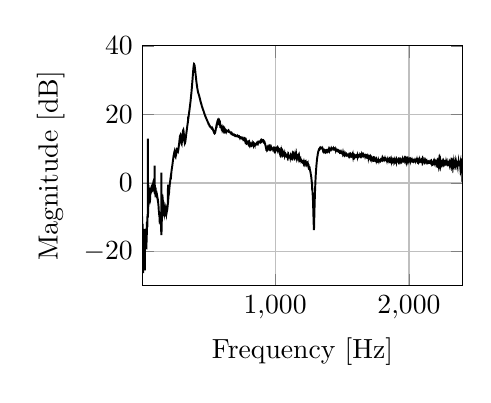
\begin{tikzpicture}

\begin{axis}[%
width=1.6in,
height=1.2in,
at={(1.011in,0.642in)},
scale only axis,
xmin=10,
xmax=2400,
xmajorgrids,
ymin=-30,
ymax=40,
ymajorgrids,
ylabel={Magnitude [dB]},
xlabel={Frequency [Hz]},
axis background/.style={fill=white}
]
\addplot [color=black,solid,line width=0.7pt,forget plot]
  table[row sep=crcr]{%
0	-19.3618707872866\\
0.666675926054529	-35.9021795514571\\
1.33335185210906	-20.4995835912269\\
2.00002777816359	-20.5444223053229\\
2.66670370421811	-9.88468154141047\\
3.33337963027264	-19.4430564977411\\
4.00005555632717	-19.9418145255131\\
4.6667314823817	-11.0447427372739\\
5.33340740843623	-16.0704359338039\\
6.00008333449076	-23.4702797128755\\
6.66675926054529	-15.6619663777543\\
7.33343518659981	-9.76687826406771\\
8.00011111265434	-19.81163092948\\
8.66678703870887	-17.2704521107206\\
9.3334629647634	-14.8299470465014\\
10.0001388908179	-20.9710252598229\\
10.6668148168725	-12.4462531922576\\
11.333490742927	-11.9282433167507\\
12.0001666689815	-20.3262262253202\\
12.666842595036	-19.7394025773231\\
13.3335185210906	-19.6473940807427\\
14.0001944471451	-26.2662831785163\\
14.6668703731996	-14.3734875190756\\
15.3335462992542	-15.6194052031707\\
16.0002222253087	-20.5496811876015\\
16.6668981513632	-22.2090559759572\\
17.3335740774177	-13.975664759218\\
18.0002500034723	-15.7219059175587\\
18.6669259295268	-18.9757168031201\\
19.3336018555813	-20.1126389030472\\
20.0002777816359	-20.0150779499674\\
20.6669537076904	-19.6692319589062\\
21.3336296337449	-20.2893657977048\\
22.0003055597994	-13.5845319182427\\
22.666981485854	-18.3651991731509\\
23.3336574119085	-18.3877906864951\\
24.000333337963	-23.6914867344971\\
24.6670092640176	-13.3952905774092\\
25.3336851900721	-14.8954912714511\\
26.0003611161266	-15.2317825176649\\
26.6670370421811	-14.3703796977619\\
27.3337129682357	-25.5165667215092\\
28.0003888942902	-13.7440540263342\\
28.6670648203447	-17.7645298009446\\
29.3337407463993	-14.7837657270799\\
30.0004166724538	-16.8735833588288\\
30.6670925985083	-17.2615490606666\\
31.3337685245628	-17.5057872025498\\
32.0004444506174	-16.2430944598921\\
32.6671203766719	-16.4407468828219\\
33.3337963027264	-17.3775675554526\\
34.000472228781	-18.1531539923639\\
34.6671481548355	-17.6636361452589\\
35.33382408089	-18.2668892181375\\
36.0005000069445	-19.3154779572481\\
36.6671759329991	-19.0730057493734\\
37.3338518590536	-17.4931961907791\\
38.0005277851081	-18.5459459068643\\
38.6672037111627	-18.5814342471402\\
39.3338796372172	-17.1293154163343\\
40.0005555632717	-17.3384234147972\\
40.6672314893262	-13.1347312756615\\
41.3339074153808	-15.5929452177734\\
42.0005833414353	-14.5776655625952\\
42.6672592674898	-11.4241252846142\\
43.3339351935444	-13.2368355069047\\
44.0006111195989	-12.2062110260313\\
44.6672870456534	-11.3220003063678\\
45.3339629717079	-12.9504502177195\\
46.0006388977625	-9.91595299096013\\
46.667314823817	-9.82517386458058\\
47.3339907498715	-10.1629820842313\\
48.0006666759261	-9.1029695267806\\
48.6673426019806	-9.80998740038481\\
49.3340185280351	-9.97000505908926\\
50.0006944540896	12.9240349727171\\
50.6673703801442	-7.21977883002444\\
51.3340463061987	-7.11446728172143\\
52.0007222322532	-8.97719564464933\\
52.6673981583078	-6.72063400953434\\
53.3340740843623	-6.3749580055128\\
54.0007500104168	-6.90631756701589\\
54.6674259364713	-6.30743722286645\\
55.3341018625259	-5.88202149675894\\
56.0007777885804	-5.61425232039832\\
56.6674537146349	-5.97918208872082\\
57.3341296406895	-5.37794492569941\\
58.000805566744	-4.89271215568237\\
58.6674814927985	-5.17338460687313\\
59.334157418853	-4.98600617637626\\
60.0008333449076	-4.85526946634448\\
60.6675092709621	-5.2761988980378\\
61.3341851970166	-3.78546843623239\\
62.0008611230712	-4.32617760644911\\
62.6675370491257	-4.54211696650046\\
63.3342129751802	-3.88517846686583\\
64.0008889012347	-4.02237599460151\\
64.6675648272893	-3.63286097665071\\
65.3342407533438	-3.87214301509673\\
66.0009166793983	-3.26523646091372\\
66.6675926054529	-3.72316484908041\\
67.3342685315074	-3.0928348687467\\
68.0009444575619	-3.24142211424055\\
68.6676203836164	-2.67465267727076\\
69.334296309671	-3.26876729871548\\
70.0009722357255	-2.63127500896192\\
70.66764816178	-2.51084178131243\\
71.3343240878346	-2.93847776060651\\
72.0010000138891	-2.31819970809246\\
72.6676759399436	-3.02553318854959\\
73.3343518659981	-2.43376505268678\\
74.0010277920527	-2.31815003861385\\
74.6677037181072	-2.31016640184259\\
75.3343796441617	-1.69491841027598\\
76.0010555702163	-2.22955738129066\\
76.6677314962708	-1.72027342301511\\
77.3344074223253	-1.6558429796661\\
78.0010833483798	-1.80714746843256\\
78.6677592744344	-1.81411401941666\\
79.3344352004889	-1.74565457439211\\
80.0011111265434	-1.52549072383373\\
80.667787052598	-1.58400244407407\\
81.3344629786525	-0.794793712460878\\
82.001138904707	-1.21720617302108\\
82.6678148307615	-1.32404377078639\\
83.3344907568161	-1.19859894415666\\
84.0011666828706	-1.54136539234771\\
84.6678426089251	-1.25417213799066\\
85.3345185349797	-1.59876693986671\\
86.0011944610342	-1.39127366917041\\
86.6678703870887	-1.3696455118177\\
87.3345463131432	-1.24349146129673\\
88.0012222391978	-1.32427084946929\\
88.6678981652523	-1.39971551325901\\
89.3345740913068	-1.17434411025682\\
90.0012500173614	-1.21083171739961\\
90.6679259434159	-1.2824931768613\\
91.3346018694704	-1.27007323884887\\
92.0012777955249	-0.966074720727181\\
92.6679537215795	-1.12262786063696\\
93.334629647634	-1.25910159242507\\
94.0013055736885	-1.00924206496683\\
94.667981499743	-1.19814649030848\\
95.3346574257976	-1.03793473306067\\
96.0013333518521	-0.985069630540586\\
96.6680092779066	-1.16576706251535\\
97.3346852039612	-1.13231955371233\\
98.0013611300157	-1.66764064822606\\
98.6680370560702	-1.28672331497108\\
99.3347129821248	-1.3445186725035\\
100.001388908179	5.03925813680822\\
100.668064834234	-1.24492409609696\\
101.334740760288	-1.84894853364229\\
102.001416686343	-1.5057135993022\\
102.668092612397	-1.62581664083084\\
103.334768538452	-1.96026321995936\\
104.001444464506	-1.80858605343605\\
104.668120390561	-1.87696249754052\\
105.334796316616	-1.77338599294492\\
106.00147224267	-1.96371233163815\\
106.668148168725	-2.43242825396346\\
107.334824094779	-1.99629794834388\\
108.001500020834	-2.07333842125666\\
108.668175946888	-2.04693878577049\\
109.334851872943	-2.7856581024142\\
110.001527798997	-2.28962283777454\\
110.668203725052	-2.82932525884246\\
111.334879651106	-2.74366176562584\\
112.001555577161	-2.77203713305229\\
112.668231503215	-2.81106168698214\\
113.33490742927	-3.29193002298192\\
114.001583355324	-2.85516807999158\\
114.668259281379	-3.25622357420913\\
115.334935207433	-2.87083513348013\\
116.001611133488	-3.20098014091963\\
116.668287059542	-3.13931560604944\\
117.334962985597	-3.21800656543537\\
118.001638911652	-3.60361366656882\\
118.668314837706	-4.17266244181744\\
119.334990763761	-3.97386570647672\\
120.001666689815	-4.10317537863612\\
120.66834261587	-4.55642386800676\\
121.335018541924	-4.25647477320912\\
122.001694467979	-4.39406873293558\\
122.668370394033	-4.51138804830031\\
123.335046320088	-4.98742159191303\\
124.001722246142	-5.14486191270147\\
124.668398172197	-4.75589633135072\\
125.335074098251	-5.43127085642699\\
126.001750024306	-5.64842885485132\\
126.66842595036	-5.30074903970846\\
127.335101876415	-6.04512020516773\\
128.001777802469	-6.29132072343327\\
128.668453728524	-6.50695924426763\\
129.335129654579	-6.82140368980889\\
130.001805580633	-7.47075787354341\\
130.668481506688	-7.55572763464663\\
131.335157432742	-8.21634295355302\\
132.001833358797	-8.32120016798544\\
132.668509284851	-8.37506524200766\\
133.335185210906	-8.9496274798399\\
134.00186113696	-9.27578626243634\\
134.668537063015	-8.80783005626224\\
135.335212989069	-9.2782531505472\\
136.001888915124	-9.64742916651176\\
136.668564841178	-9.46825003491031\\
137.335240767233	-10.4050921542696\\
138.001916693287	-11.3250511085103\\
138.668592619342	-11.5516815812687\\
139.335268545396	-11.1106617083089\\
140.001944471451	-11.7499094291161\\
140.668620397506	-10.1510233892866\\
141.33529632356	-11.157217772991\\
142.001972249615	-10.2106984049837\\
142.668648175669	-10.0510334437557\\
143.335324101724	-10.3268554510805\\
144.002000027778	-10.0355459586078\\
144.668675953833	-10.7763809377099\\
145.335351879887	-10.8587694825624\\
146.002027805942	-10.4799795322674\\
146.668703731996	-11.4493056473397\\
147.335379658051	-12.1437142770862\\
148.002055584105	-11.962164877165\\
148.66873151016	-13.5416518045528\\
149.335407436214	-14.1889118439315\\
150.002083362269	3.04128722772059\\
150.668759288323	-15.1869062815816\\
151.335435214378	-13.7380737628693\\
152.002111140433	-14.2196536995097\\
152.668787066487	-13.4046421317761\\
153.335462992542	-11.6471719266991\\
154.002138918596	-10.760690485525\\
154.668814844651	-8.41691304980566\\
155.335490770705	-7.38533557911436\\
156.00216669676	-6.02064320421254\\
156.668842622814	-5.46287813346268\\
157.335518548869	-5.04969251448635\\
158.002194474923	-4.50630124511883\\
158.668870400978	-4.43783654221954\\
159.335546327032	-4.88720353680776\\
160.002222253087	-5.06977429115913\\
160.668898179141	-5.19068972670615\\
161.335574105196	-5.64099493735669\\
162.00225003125	-5.56196878479219\\
162.668925957305	-6.01141409718634\\
163.335601883359	-6.75241892022081\\
164.002277809414	-6.538990401781\\
164.668953735469	-7.23450154339778\\
165.335629661523	-6.74809548714496\\
166.002305587578	-7.05029257720258\\
166.668981513632	-7.39507165753175\\
167.335657439687	-7.48702815002829\\
168.002333365741	-8.58992278330363\\
168.669009291796	-8.52914852452159\\
169.33568521785	-8.6499350226437\\
170.002361143905	-7.8212165466623\\
170.669037069959	-7.89120213363103\\
171.335712996014	-8.07367011944289\\
172.002388922068	-7.87410609432333\\
172.669064848123	-8.17219993186708\\
173.335740774177	-7.76390095527525\\
174.002416700232	-8.28752825751316\\
174.669092626286	-9.02660428520083\\
175.335768552341	-8.49123820860328\\
176.002444478396	-9.17787961327407\\
176.66912040445	-8.95991283252426\\
177.335796330505	-8.76127455026899\\
178.002472256559	-9.04680280690476\\
178.669148182614	-9.00947111443036\\
179.335824108668	-9.31841804953383\\
180.002500034723	-9.27939456248399\\
180.669175960777	-8.71202583157834\\
181.335851886832	-9.50555929637702\\
182.002527812886	-8.65467993330737\\
182.669203738941	-8.62737799434884\\
183.335879664995	-9.25840518347694\\
184.00255559105	-9.04713806452003\\
184.669231517104	-8.5769430502273\\
185.335907443159	-8.67916420279669\\
186.002583369213	-8.26380700268637\\
186.669259295268	-8.42703416133062\\
187.335935221323	-7.99077751566202\\
188.002611147377	-8.43371721076821\\
188.669287073432	-8.37654035264563\\
189.335962999486	-8.22655884060956\\
190.002638925541	-8.24542965380036\\
190.669314851595	-8.29516042022565\\
191.33599077765	-8.26974793241131\\
192.002666703704	-7.82383305400602\\
192.669342629759	-8.08518583158324\\
193.336018555813	-7.94370588210414\\
194.002694481868	-7.93350967469461\\
194.669370407922	-7.70096143221432\\
195.336046333977	-7.50573609828088\\
196.002722260031	-7.29973916755475\\
196.669398186086	-7.03754494912687\\
197.33607411214	-6.85627051694723\\
198.002750038195	-6.35118374603092\\
198.66942596425	-6.27329248670784\\
199.336101890304	-5.62064545943526\\
200.002777816359	-0.520653736743226\\
200.669453742413	-5.75155877791724\\
201.336129668468	-4.4796134774656\\
202.002805594522	-4.72430752959396\\
202.669481520577	-4.45546021526977\\
203.336157446631	-3.75557102781182\\
204.002833372686	-3.8760403407913\\
204.66950929874	-3.58209516706976\\
205.336185224795	-3.07413435211663\\
206.002861150849	-3.40025646658202\\
206.669537076904	-2.69080359845468\\
207.336213002958	-2.45267696602557\\
208.002888929013	-2.27657737542287\\
208.669564855067	-2.00718168263896\\
209.336240781122	-2.04701852008489\\
210.002916707176	-1.69324008482576\\
210.669592633231	-1.37541420512163\\
211.336268559286	-1.13288083349977\\
212.00294448534	-0.978882286512991\\
212.669620411395	-0.702656183358659\\
213.336296337449	-0.417395694808079\\
214.002972263504	-0.0938414326463799\\
214.669648189558	-0.0327216465792262\\
215.336324115613	0.148708855407083\\
216.003000041667	0.353599018349351\\
216.669675967722	0.640722273963735\\
217.336351893776	0.915434231330508\\
218.003027819831	1.08714478615943\\
218.669703745885	1.35820861389876\\
219.33637967194	1.39138473536075\\
220.003055597994	1.58445637848068\\
220.669731524049	1.92489091425733\\
221.336407450103	2.08392184258553\\
222.003083376158	2.29463658656951\\
222.669759302213	2.38872420024993\\
223.336435228267	2.32391680605784\\
224.003111154322	2.75108126293096\\
224.669787080376	2.85452164625662\\
225.336463006431	3.11943011750765\\
226.003138932485	3.25625659268346\\
226.66981485854	3.61479060230108\\
227.336490784594	3.78807072357767\\
228.003166710649	3.95529919063432\\
228.669842636703	4.16890859721735\\
229.336518562758	4.27608573371528\\
230.003194488812	4.45094403532182\\
230.669870414867	4.75972997884267\\
231.336546340921	4.81041865641967\\
232.003222266976	5.01992162693982\\
232.66989819303	5.1368566929275\\
233.336574119085	5.37977685110137\\
234.00325004514	5.57911241316725\\
234.669925971194	5.886281344509\\
235.336601897249	5.95716756450319\\
236.003277823303	6.24665076575757\\
236.669953749358	6.48035740261547\\
237.336629675412	6.59231804135953\\
238.003305601467	6.7595849546891\\
238.669981527521	6.96399230087505\\
239.336657453576	7.18840104598157\\
240.00333337963	7.34042905452338\\
240.670009305685	7.52067395403219\\
241.336685231739	7.78622676943283\\
242.003361157794	7.92212176337835\\
242.670037083848	8.02632475838035\\
243.336713009903	8.24755980034838\\
244.003388935957	8.31487755452782\\
244.670064862012	8.470129661696\\
245.336740788066	8.54651053668772\\
246.003416714121	8.66806739733013\\
246.670092640176	8.83423476835627\\
247.33676856623	8.86612833832024\\
248.003444492285	9.07134124641547\\
248.670120418339	9.19343952631\\
249.336796344394	9.23323500853091\\
250.003472270448	9.32917023555425\\
250.670148196503	9.22395032652007\\
251.336824122557	9.13451808256684\\
252.003500048612	9.08731067564757\\
252.670175974666	8.79771825972886\\
253.336851900721	8.47691499356256\\
254.003527826775	8.19265450674294\\
254.67020375283	8.11053299755807\\
255.336879678884	7.8776402441604\\
256.003555604939	7.79160855896555\\
256.670231530993	7.83822328837478\\
257.336907457048	7.76763923640498\\
258.003583383103	7.91120444175719\\
258.670259309157	7.91612951645949\\
259.336935235212	8.06824101762504\\
260.003611161266	8.07494836406927\\
260.670287087321	8.23213331881161\\
261.336963013375	8.35977759477462\\
262.00363893943	8.62660813340609\\
262.670314865484	8.76475356215733\\
263.336990791539	9.00975952747425\\
264.003666717593	9.2256387347976\\
264.670342643648	9.41713264155132\\
265.337018569702	9.59861537432747\\
266.003694495757	9.55659118309994\\
266.670370421811	9.69957805668921\\
267.337046347866	9.66825541135089\\
268.00372227392	9.79519246191875\\
268.670398199975	9.80416559193101\\
269.33707412603	9.82703383043057\\
270.003750052084	9.68425574584365\\
270.670425978139	9.55682305741921\\
271.337101904193	9.41527968725362\\
272.003777830248	9.35609483611069\\
272.670453756302	9.24650902633177\\
273.337129682357	9.21320342348463\\
274.003805608411	9.20658559249051\\
274.670481534466	9.1675925688572\\
275.33715746052	9.30950450253818\\
276.003833386575	9.40606610828403\\
276.670509312629	9.57354347722375\\
277.337185238684	9.65703031885105\\
278.003861164738	9.96843184510568\\
278.670537090793	10.109811346222\\
279.337213016847	10.2745766901816\\
280.003888942902	10.493837169901\\
280.670564868956	10.7057934412898\\
281.337240795011	10.9513089721492\\
282.003916721066	11.1196552776977\\
282.67059264712	11.3770962150196\\
283.337268573175	11.5223683607698\\
284.003944499229	11.7237586181509\\
284.670620425284	12.0345613251209\\
285.337296351338	12.2703988487711\\
286.003972277393	12.5279272205309\\
286.670648203447	12.7416227815932\\
287.337324129502	12.9073142387462\\
288.004000055556	13.1180975787029\\
288.670675981611	13.333831397237\\
289.337351907665	13.5670474406913\\
290.00402783372	13.6373832842423\\
290.670703759774	13.7336113664837\\
291.337379685829	13.8146802869948\\
292.004055611883	13.8867266611167\\
292.670731537938	13.9426041891924\\
293.337407463993	13.7950036884169\\
294.004083390047	13.7070665226796\\
294.670759316102	13.5445840514981\\
295.337435242156	13.308689775809\\
296.004111168211	13.0440508478036\\
296.670787094265	12.7680920257627\\
297.33746302032	12.4142136041678\\
298.004138946374	12.2450852754287\\
298.670814872429	11.9564549319363\\
299.337490798483	11.6258386404829\\
300.004166724538	12.2684439114719\\
300.670842650592	11.6229937666425\\
301.337518576647	11.4374183909306\\
302.004194502701	11.3813821254475\\
302.670870428756	11.6490669280708\\
303.33754635481	11.8056923728049\\
304.004222280865	11.9167095181664\\
304.67089820692	12.1013743018492\\
305.337574132974	12.4757414084964\\
306.004250059029	12.6877860532945\\
306.670925985083	12.9221839479462\\
307.337601911138	13.2515852007202\\
308.004277837192	13.6256753511003\\
308.670953763247	13.7629636930123\\
309.337629689301	14.0857124478674\\
310.004305615356	14.4385359063525\\
310.67098154141	14.6574312831774\\
311.337657467465	14.7989979451058\\
312.004333393519	15.1433103039367\\
312.671009319574	15.300451077485\\
313.337685245628	15.3596258012415\\
314.004361171683	15.4610068622099\\
314.671037097737	15.5093536938561\\
315.337713023792	15.3241037375253\\
316.004388949847	15.1987447944542\\
316.671064875901	15.0418771577208\\
317.337740801956	14.705894533561\\
318.00441672801	14.4189846794481\\
318.671092654065	14.071762199169\\
319.337768580119	13.6736985288621\\
320.004444506174	13.3741171124124\\
320.671120432228	13.1263467212002\\
321.337796358283	12.7215684804356\\
322.004472284337	12.4631415681196\\
322.671148210392	12.2463477055507\\
323.337824136446	12.0011302606234\\
324.004500062501	11.8984163784686\\
324.671175988555	11.7539313190426\\
325.33785191461	11.6269151414737\\
326.004527840664	11.7039112439033\\
326.671203766719	11.6990518883027\\
327.337879692774	11.6892884983601\\
328.004555618828	11.8944320306926\\
328.671231544883	11.9053719841116\\
329.337907470937	12.0472273530908\\
330.004583396992	12.2509789817655\\
330.671259323046	12.3680599176696\\
331.337935249101	12.638658943634\\
332.004611175155	12.7793608680765\\
332.67128710121	13.0093969748005\\
333.337963027264	13.2479431438629\\
334.004638953319	13.3902878141347\\
334.671314879373	13.6414326564039\\
335.337990805428	13.8752340445966\\
336.004666731482	14.072334978583\\
336.671342657537	14.3178892978025\\
337.338018583591	14.4548758441018\\
338.004694509646	14.7313876890009\\
338.671370435701	14.895318907374\\
339.338046361755	15.0835656030104\\
340.00472228781	15.3484762287606\\
340.671398213864	15.4749435079211\\
341.338074139919	15.7885587498514\\
342.004750065973	15.8653297787316\\
342.671425992028	16.1692239080047\\
343.338101918082	16.3364392416717\\
344.004777844137	16.5375356826601\\
344.671453770191	16.7465089878244\\
345.338129696246	16.8689924903991\\
346.0048056223	17.1428477313714\\
346.671481548355	17.2224447025625\\
347.338157474409	17.5285110516813\\
348.004833400464	17.6448279591173\\
348.671509326518	17.8805075734288\\
349.338185252573	18.0337037472689\\
350.004861178627	18.4750360674794\\
350.671537104682	18.4271588641798\\
351.338213030737	18.6396716938208\\
352.004888956791	18.817678443432\\
352.671564882846	19.0002002370105\\
353.3382408089	19.2145298232811\\
354.004916734955	19.3697422309362\\
354.671592661009	19.650137471914\\
355.338268587064	19.773616656178\\
356.004944513118	20.0281417507844\\
356.671620439173	20.1588654093105\\
357.338296365227	20.4255123616847\\
358.004972291282	20.5303176375592\\
358.671648217336	20.7990100777883\\
359.338324143391	20.9091847448413\\
360.005000069445	21.2009998211123\\
360.6716759955	21.3288520965485\\
361.338351921554	21.5974520900444\\
362.005027847609	21.7406101663951\\
362.671703773664	22.0036786609798\\
363.338379699718	22.1758939389062\\
364.005055625773	22.4092065617165\\
364.671731551827	22.6043360131825\\
365.338407477882	22.8145214531445\\
366.005083403936	23.0617249493562\\
366.671759329991	23.2383753963735\\
367.338435256045	23.5017511838225\\
368.0051111821	23.6618519776456\\
368.671787108154	23.977567524018\\
369.338463034209	24.1377164918625\\
370.005138960263	24.4722243451756\\
370.671814886318	24.6391151153694\\
371.338490812372	24.9651881333226\\
372.005166738427	25.1941275253484\\
372.671842664481	25.4573765925804\\
373.338518590536	25.7351898199429\\
374.005194516591	25.9486361440607\\
374.671870442645	26.2832248300519\\
375.3385463687	26.4693507438062\\
376.005222294754	26.8144423497695\\
376.671898220809	27.0407559976594\\
377.338574146863	27.3701293895772\\
378.005250072918	27.680314120169\\
378.671925998972	27.9504246390054\\
379.338601925027	28.3454701276926\\
380.005277851081	28.5897427933487\\
380.671953777136	28.9598274560529\\
381.33862970319	29.2536896482888\\
382.005305629245	29.5453436058301\\
382.671981555299	29.9355965603662\\
383.338657481354	30.1901741693537\\
384.005333407408	30.6024607334653\\
384.672009333463	30.9408032580226\\
385.338685259517	31.2464303425154\\
386.005361185572	31.6582574166453\\
386.672037111627	31.9166682784181\\
387.338713037681	32.274553603347\\
388.005388963736	32.6352470836804\\
388.67206488979	32.8866022402636\\
389.338740815845	33.274612379558\\
390.005416741899	33.5224629896123\\
390.672092667954	33.7326211728478\\
391.338768594008	34.0294594929755\\
392.005444520063	34.1528217813387\\
392.672120446117	34.3275564638173\\
393.338796372172	34.4921494668572\\
394.005472298226	34.4524799900155\\
394.672148224281	34.5059415132715\\
395.338824150335	34.5379844686153\\
396.00550007639	34.4529508200051\\
396.672176002444	34.4829120732413\\
397.338851928499	34.4345855545715\\
398.005527854554	34.27809377157\\
398.672203780608	34.2568437771917\\
399.338879706663	34.150150332169\\
400.005555632717	33.8825667999354\\
400.672231558772	33.7079545246617\\
401.338907484826	33.5456191717806\\
402.005583410881	33.2569646041632\\
402.672259336935	33.0118281021832\\
403.33893526299	32.8101399600196\\
404.005611189044	32.5135652481275\\
404.672287115099	32.2724666422037\\
405.338963041153	32.0603665146494\\
406.005638967208	31.7709155855659\\
406.672314893262	31.5044802920053\\
407.338990819317	31.3132797832042\\
408.005666745371	31.065515456776\\
408.672342671426	30.7580187562882\\
409.339018597481	30.5580858508745\\
410.005694523535	30.3814806356686\\
410.67237044959	30.0840019715765\\
411.339046375644	29.8351961702988\\
412.005722301699	29.7017199577745\\
412.672398227753	29.4682927059066\\
413.339074153808	29.194237507581\\
414.005750079862	29.0338915668757\\
414.672426005917	28.8537213867012\\
415.339101931971	28.6409556880654\\
416.005777858026	28.4209807945455\\
416.67245378408	28.2303070369924\\
417.339129710135	28.10569740321\\
418.005805636189	27.9013742615739\\
418.672481562244	27.6773246424915\\
419.339157488298	27.5411580665293\\
420.005833414353	27.4461017056009\\
420.672509340407	27.2479285245684\\
421.339185266462	27.0386024971026\\
422.005861192517	26.9571503298195\\
422.672537118571	26.8396501979411\\
423.339213044626	26.7515608658471\\
424.00588897068	26.5615335036433\\
424.672564896735	26.4335183800764\\
425.339240822789	26.3898871635666\\
426.005916748844	26.3303199681989\\
426.672592674898	26.1673378111597\\
427.339268600953	26.0862711715932\\
428.005944527007	25.9948121779699\\
428.672620453062	25.9758807816233\\
429.339296379116	25.8911701560308\\
430.005972305171	25.7621120146669\\
430.672648231225	25.6623947562977\\
431.33932415728	25.5856764220714\\
432.006000083334	25.5443756100151\\
432.672676009389	25.4873050488812\\
433.339351935444	25.3240776275726\\
434.006027861498	25.2329882518413\\
434.672703787553	25.0844787960022\\
435.339379713607	25.073088832736\\
436.006055639662	24.9697441411312\\
436.672731565716	24.8721485403557\\
437.339407491771	24.7170291418084\\
438.006083417825	24.5580523600165\\
438.67275934388	24.4958749979621\\
439.339435269934	24.3796001834163\\
440.006111195989	24.3511004999882\\
440.672787122043	24.1954836461562\\
441.339463048098	24.0752971763901\\
442.006138974152	23.9383321411095\\
442.672814900207	23.8441399968708\\
443.339490826261	23.7755733812962\\
444.006166752316	23.7002205221968\\
444.672842678371	23.6007989924081\\
445.339518604425	23.5099756219178\\
446.00619453048	23.3793801644176\\
446.672870456534	23.2498904206607\\
447.339546382589	23.1675170539806\\
448.006222308643	23.0814009437549\\
448.672898234698	23.0116942793781\\
449.339574160752	22.964840851347\\
450.006250086807	22.9458704611028\\
450.672926012861	22.7783538254155\\
451.339601938916	22.6382110135418\\
452.00627786497	22.5476970468293\\
452.672953791025	22.4317637900438\\
453.339629717079	22.3681217755119\\
454.006305643134	22.2761764703997\\
454.672981569188	22.2294736097782\\
455.339657495243	22.1449451202068\\
456.006333421298	22.1160098296591\\
456.673009347352	22.0060886937568\\
457.339685273407	21.9304768469233\\
458.006361199461	21.8244093856888\\
458.673037125516	21.7316223491682\\
459.33971305157	21.6257007503832\\
460.006388977625	21.5309560014764\\
460.673064903679	21.4782096457126\\
461.339740829734	21.4014578573023\\
462.006416755788	21.3592599180213\\
462.673092681843	21.256840338377\\
463.339768607897	21.2065775637823\\
464.006444533952	21.1350130881169\\
464.673120460006	21.0839212617895\\
465.339796386061	21.0055807317284\\
466.006472312115	20.9206656945536\\
466.67314823817	20.8391310697489\\
467.339824164225	20.7488575893734\\
468.006500090279	20.6839066870886\\
468.673176016334	20.6176278655441\\
469.339851942388	20.515563407399\\
470.006527868443	20.4489964588962\\
470.673203794497	20.3415372715676\\
471.339879720552	20.2434423446577\\
472.006555646606	20.2238547972236\\
472.673231572661	20.1500104700638\\
473.339907498715	20.0641149313031\\
474.00658342477	20.0155520841237\\
474.673259350824	19.8984088787438\\
475.339935276879	19.8167830452497\\
476.006611202933	19.7829865189436\\
476.673287128988	19.6697896991569\\
477.339963055042	19.5995051883076\\
478.006638981097	19.5952348274665\\
478.673314907152	19.5014798057631\\
479.339990833206	19.4176958625874\\
480.006666759261	19.3725855091289\\
480.673342685315	19.2757692541619\\
481.34001861137	19.2196493243922\\
482.006694537424	19.2042050143783\\
482.673370463479	19.0951235276728\\
483.340046389533	19.0102230895272\\
484.006722315588	18.9773397078674\\
484.673398241642	18.9312526849428\\
485.340074167697	18.8557475227714\\
486.006750093751	18.7949903251266\\
486.673426019806	18.7466929988789\\
487.34010194586	18.690511732119\\
488.006777871915	18.6189838500254\\
488.673453797969	18.5860954078857\\
489.340129724024	18.5331296321922\\
490.006805650078	18.4579266990112\\
490.673481576133	18.372315235375\\
491.340157502188	18.3319678573866\\
492.006833428242	18.2823146786698\\
492.673509354297	18.1736580621393\\
493.340185280351	18.1154465819649\\
494.006861206406	18.0874254414673\\
494.67353713246	17.9971101242718\\
495.340213058515	17.9153642911631\\
496.006888984569	17.8558607499057\\
496.673564910624	17.8272089195585\\
497.340240836678	17.7689684682805\\
498.006916762733	17.7240616823976\\
498.673592688787	17.6788090881146\\
499.340268614842	17.6161004207237\\
500.006944540896	17.5310425513652\\
500.673620466951	17.4425271469796\\
501.340296393005	17.3418460395877\\
502.00697231906	17.2758221677175\\
502.673648245115	17.267028255022\\
503.340324171169	17.2781276668744\\
504.007000097224	17.210917417503\\
504.673676023278	17.1200646646595\\
505.340351949333	17.1059976868596\\
506.007027875387	17.1007664238695\\
506.673703801442	17.0331785872377\\
507.340379727496	16.9913466987233\\
508.007055653551	16.8890069270035\\
508.673731579605	16.7891066779324\\
509.34040750566	16.7300467123014\\
510.007083431714	16.7381196955819\\
510.673759357769	16.7328369246324\\
511.340435283823	16.7169103707291\\
512.007111209878	16.6382801236244\\
512.673787135932	16.547096015275\\
513.340463061987	16.4854386771388\\
514.007138988041	16.4542937923094\\
514.673814914096	16.4454673311036\\
515.340490840151	16.4489332837606\\
516.007166766205	16.4147961994688\\
516.67384269226	16.3885516307465\\
517.340518618314	16.2706279815487\\
518.007194544369	16.2591221149596\\
518.673870470423	16.233324992577\\
519.340546396478	16.244104383152\\
520.007222322532	16.2195029701752\\
520.673898248587	16.1556079743307\\
521.340574174641	16.1440169406125\\
522.007250100696	16.1674559478337\\
522.67392602675	16.1547922202727\\
523.340601952805	16.1554122758746\\
524.007277878859	16.152751152871\\
524.673953804914	16.1225027133183\\
525.340629730968	16.0499008571852\\
526.007305657023	16.0795852066358\\
526.673981583078	16.1017003009515\\
527.340657509132	16.0856263004078\\
528.007333435187	16.0056037949166\\
528.674009361241	15.9978384794813\\
529.340685287296	15.9499654219996\\
530.00736121335	16.003658067844\\
530.674037139405	15.9471291338518\\
531.340713065459	15.8773895206512\\
532.007388991514	15.8553531599656\\
532.674064917568	15.8745775444435\\
533.340740843623	15.8172777924018\\
534.007416769677	15.751167853204\\
534.674092695732	15.647045896088\\
535.340768621786	15.6247740794223\\
536.007444547841	15.582567223678\\
536.674120473896	15.4662287045036\\
537.34079639995	15.3955257377633\\
538.007472326005	15.3540519147725\\
538.674148252059	15.3184859454046\\
539.340824178114	15.2142494108425\\
540.007500104168	15.0955185860154\\
540.674176030223	15.062525615901\\
541.340851956277	15.0007524619735\\
542.007527882332	14.9025895827768\\
542.674203808386	14.8018046876672\\
543.340879734441	14.7850196988538\\
544.007555660495	14.7340519595461\\
544.67423158655	14.6269471808843\\
545.340907512604	14.6217859780869\\
546.007583438659	14.5934141185214\\
546.674259364713	14.534385789673\\
547.340935290768	14.4938739308286\\
548.007611216823	14.5311076929047\\
548.674287142877	14.5753219172441\\
549.340963068932	14.4832816844596\\
550.007638994986	14.5024924292087\\
550.674314921041	14.6453692764469\\
551.340990847095	14.6303311481102\\
552.00766677315	14.7006516644172\\
552.674342699204	14.8781835538091\\
553.341018625259	14.8764908876774\\
554.007694551313	14.995040459506\\
554.674370477368	15.1276311512138\\
555.341046403422	15.2651930513634\\
556.007722329477	15.4016446287971\\
556.674398255531	15.5902671350371\\
557.341074181586	15.7385518181621\\
558.00775010764	15.8431428971125\\
558.674426033695	16.0986336876973\\
559.341101959749	16.2007778182753\\
560.007777885804	16.2836797149855\\
560.674453811858	16.5437508861976\\
561.341129737913	16.5899679771811\\
562.007805663968	16.7156325267429\\
562.674481590022	16.9194361753216\\
563.341157516077	16.9085567183153\\
564.007833442131	17.1211072544243\\
564.674509368186	17.1512557343425\\
565.34118529424	17.0857459059384\\
566.007861220295	17.3069040450994\\
566.674537146349	17.4528274790765\\
567.341213072404	17.5256146547363\\
568.007888998458	17.6918720512982\\
568.674564924513	17.6703158465671\\
569.341240850567	17.7938311019778\\
570.007916776622	17.8906645467607\\
570.674592702676	17.826349172351\\
571.341268628731	17.9664138185063\\
572.007944554785	17.966508251008\\
572.67462048084	17.9574442607058\\
573.341296406895	18.0296151345562\\
574.007972332949	17.999888482376\\
574.674648259004	18.106721858489\\
575.341324185058	18.059163234698\\
576.008000111113	18.0474279390616\\
576.674676037167	18.0904361152733\\
577.341351963222	17.9682624220956\\
578.008027889276	18.0611991994242\\
578.674703815331	17.9689211591393\\
579.341379741385	17.9958547488359\\
580.00805566744	17.9259833215245\\
580.674731593494	17.8496803933777\\
581.341407519549	17.9143362018226\\
582.008083445603	17.7492996791415\\
582.674759371658	17.8030287711394\\
583.341435297712	17.6432104530114\\
584.008111223767	17.6781893434403\\
584.674787149822	17.5529599100494\\
585.341463075876	17.5158046063981\\
586.008139001931	17.5143171799659\\
586.674814927985	17.358332057589\\
587.34149085404	17.3509933314181\\
588.008166780094	17.1707471744715\\
588.674842706149	17.2378131402912\\
589.341518632203	17.0291383177995\\
590.008194558258	17.0820169695886\\
590.674870484312	16.8696166053489\\
591.341546410367	16.8689438635772\\
592.008222336421	16.6909351796721\\
592.674898262476	16.7283398771291\\
593.34157418853	16.6093793369855\\
594.008250114585	16.5725131254014\\
594.674926040639	16.489629826362\\
595.341601966694	16.4613662983083\\
596.008277892749	16.3360261545365\\
596.674953818803	16.2886794174475\\
597.341629744858	16.2324550134901\\
598.008305670912	16.1744263898047\\
598.674981596967	16.079717588956\\
599.341657523021	16.1259435635265\\
600.008333449076	15.9767148955137\\
600.67500937513	16.0139479376889\\
601.341685301185	15.9254718077809\\
602.008361227239	15.9435933343133\\
602.675037153294	15.8624794178313\\
603.341713079348	15.906156928152\\
604.008389005403	15.7747610080793\\
604.675064931457	15.8888550080739\\
605.341740857512	15.761247222628\\
606.008416783566	15.8165923481738\\
606.675092709621	15.7496528386067\\
607.341768635676	15.7508714646688\\
608.00844456173	15.6857656912273\\
608.675120487785	15.7167625244519\\
609.341796413839	15.6995488269068\\
610.008472339894	15.6424265324421\\
610.675148265948	15.6646889860933\\
611.341824192003	15.5981063503046\\
612.008500118057	15.6954236013886\\
612.675176044112	15.5575633767151\\
613.341851970166	15.6133037649105\\
614.008527896221	15.5459740740405\\
614.675203822275	15.5504160664722\\
615.34187974833	15.5655742560186\\
616.008555674384	15.4618995923198\\
616.675231600439	15.5687384925729\\
617.341907526493	15.4737390839156\\
618.008583452548	15.5199889963706\\
618.675259378603	15.4965481480473\\
619.341935304657	15.4710211904958\\
620.008611230711	15.50636608978\\
620.675287156766	15.3896184829142\\
621.341963082821	15.4296222622508\\
622.008639008875	15.406192517108\\
622.67531493493	15.3170342522488\\
623.341990860984	15.4162122020578\\
624.008666787039	15.2830087759572\\
624.675342713093	15.2979620938838\\
625.342018639148	15.3215521484245\\
626.008694565202	15.2020027546952\\
626.675370491257	15.2603739246503\\
627.342046417311	15.1819334534858\\
628.008722343366	15.1829092050369\\
628.67539826942	15.2310981588317\\
629.342074195475	15.1424132219261\\
630.008750121529	15.1299404551401\\
630.675426047584	15.1044124484591\\
631.342101973638	15.0384233724096\\
632.008777899693	15.0628907154921\\
632.675453825748	15.0643895175643\\
633.342129751802	14.991755602926\\
634.008805677857	15.0289376836571\\
634.675481603911	14.9567612139926\\
635.342157529966	15.0404620075365\\
636.00883345602	15.0039848712989\\
636.675509382075	15.0038177581841\\
637.342185308129	15.0024032748583\\
638.008861234184	15.05293545392\\
638.675537160238	14.9832680858656\\
639.342213086293	14.9901300836212\\
640.008889012347	15.0591159996423\\
640.675564938402	15.044859025629\\
641.342240864456	15.083351266305\\
642.008916790511	15.1263758033044\\
642.675592716565	15.1028332768199\\
643.34226864262	15.1055323300386\\
644.008944568675	15.1209244741918\\
644.675620494729	15.1658218038784\\
645.342296420784	15.1515474544963\\
646.008972346838	15.1795048076326\\
646.675648272893	15.1905055639529\\
647.342324198947	15.1396839278998\\
648.009000125002	15.1375807670928\\
648.675676051056	15.178874057423\\
649.342351977111	15.2010996414745\\
650.009027903165	15.1899210122617\\
650.67570382922	15.1515109708583\\
651.342379755274	15.195063979341\\
652.009055681329	15.1197695293232\\
652.675731607383	15.1109590932212\\
653.342407533438	15.1430706776879\\
654.009083459492	15.060146027094\\
654.675759385547	15.0397822060428\\
655.342435311602	15.0136621212574\\
656.009111237656	15.0264153167971\\
656.675787163711	15.0010667411867\\
657.342463089765	14.9359942129756\\
658.00913901582	14.9456725312995\\
658.675814941874	14.937564205371\\
659.342490867929	14.9330347757354\\
660.009166793983	14.8476593767594\\
660.675842720038	14.8298010178927\\
661.342518646092	14.8521411911059\\
662.009194572147	14.8138021405902\\
662.675870498201	14.7799592033147\\
663.342546424256	14.7602882786645\\
664.00922235031	14.7843995700771\\
664.675898276365	14.7613031185636\\
665.342574202419	14.6997739103442\\
666.009250128474	14.647849207414\\
666.675926054529	14.6741076767612\\
667.342601980583	14.658983418656\\
668.009277906638	14.6340029278413\\
668.675953832692	14.5802675738556\\
669.342629758747	14.5500436678723\\
670.009305684801	14.526178486487\\
670.675981610856	14.5394770773497\\
671.34265753691	14.5219385320991\\
672.009333462965	14.4986132756945\\
672.676009389019	14.4352178124029\\
673.342685315074	14.4485954476707\\
674.009361241128	14.4878402138349\\
674.676037167183	14.4013804107998\\
675.342713093237	14.4192010349633\\
676.009389019292	14.3625027237386\\
676.676064945346	14.343631158623\\
677.342740871401	14.3402153760337\\
678.009416797456	14.3082554796504\\
678.67609272351	14.3442732888289\\
679.342768649565	14.2861876061887\\
680.009444575619	14.2689792423788\\
680.676120501674	14.2123174718637\\
681.342796427728	14.2336900519799\\
682.009472353783	14.238650398911\\
682.676148279837	14.2133455917976\\
683.342824205892	14.2244965388138\\
684.009500131946	14.1629816041953\\
684.676176058001	14.1302589440397\\
685.342851984055	14.1066697218618\\
686.00952791011	14.1357085205693\\
686.676203836164	14.102929134461\\
687.342879762219	14.1359172429107\\
688.009555688273	14.1156655571112\\
688.676231614328	14.0913762570809\\
689.342907540382	14.029543568363\\
690.009583466437	14.0179752259669\\
690.676259392492	14.0016672403027\\
691.342935318546	14.0045088610928\\
692.009611244601	14.0253395338315\\
692.676287170655	13.9844126382275\\
693.34296309671	13.9683046235232\\
694.009639022764	13.985898212397\\
694.676314948819	13.9584388282645\\
695.342990874873	13.9291291440968\\
696.009666800928	13.958451935271\\
696.676342726982	13.921909930188\\
697.343018653037	13.8815257231815\\
698.009694579091	13.8551671378551\\
698.676370505146	13.8318432190888\\
699.3430464312	13.8788000375133\\
700.009722357255	13.8386692913296\\
700.676398283309	13.8642243706605\\
701.343074209364	13.8919960314968\\
702.009750135419	13.8970949708776\\
702.676426061473	13.908649011525\\
703.343101987528	13.867472690205\\
704.009777913582	13.8472921888497\\
704.676453839637	13.8153997187105\\
705.343129765691	13.8194229330283\\
706.009805691746	13.8193839467886\\
706.6764816178	13.7576744413756\\
707.343157543855	13.7281335630431\\
708.009833469909	13.7581090389923\\
708.676509395964	13.7336444513536\\
709.343185322018	13.7368958052653\\
710.009861248073	13.7404630204994\\
710.676537174127	13.720487741455\\
711.343213100182	13.7038925605696\\
712.009889026236	13.7181577154569\\
712.676564952291	13.7335300093784\\
713.343240878346	13.7577661581475\\
714.0099168044	13.7601406807116\\
714.676592730455	13.7366848146595\\
715.343268656509	13.7165988254693\\
716.009944582564	13.7062605715623\\
716.676620508618	13.7301886799278\\
717.343296434673	13.6846240935792\\
718.009972360727	13.6841924107272\\
718.676648286782	13.7175729878836\\
719.343324212836	13.6415952930352\\
720.010000138891	13.6483893505625\\
720.676676064945	13.6483449021777\\
721.343351991	13.6215366069217\\
722.010027917054	13.6291236851842\\
722.676703843109	13.654633097726\\
723.343379769163	13.6096098008079\\
724.010055695218	13.5721151672515\\
724.676731621273	13.5858637068171\\
725.343407547327	13.5478677057616\\
726.010083473382	13.5696625277931\\
726.676759399436	13.5325465036717\\
727.343435325491	13.5615185372619\\
728.010111251545	13.5466849020637\\
728.6767871776	13.5685429756374\\
729.343463103654	13.5786128955822\\
730.010139029709	13.5405076255293\\
730.676814955763	13.5675248733976\\
731.343490881818	13.5860519296907\\
732.010166807872	13.5335257802545\\
732.676842733927	13.4821114190032\\
733.343518659981	13.4454154861402\\
734.010194586036	13.3868015219426\\
734.67687051209	13.3644298004664\\
735.343546438145	13.3412333772738\\
736.0102223642	13.3290768855355\\
736.676898290254	13.259861063814\\
737.343574216309	13.3489657320765\\
738.010250142363	13.3250303096578\\
738.676926068418	13.346910397895\\
739.343601994472	13.3460464182725\\
740.010277920527	13.3451647607941\\
740.676953846581	13.2743684872826\\
741.343629772636	13.2017987113616\\
742.01030569869	13.1174332027916\\
742.676981624745	13.1181665794177\\
743.343657550799	13.1619966972896\\
744.010333476854	13.2088612653572\\
744.677009402908	13.1827927301895\\
745.343685328963	13.1677012226232\\
746.010361255017	13.1204129038755\\
746.677037181072	13.1066997017076\\
747.343713107127	13.0779342325855\\
748.010389033181	13.027765696596\\
748.677064959236	13.0200117247697\\
749.34374088529	13.0515695854367\\
750.010416811345	13.1011932069225\\
750.677092737399	13.0765327786098\\
751.343768663454	13.062743954509\\
752.010444589508	13.0234907363263\\
752.677120515563	12.915229297473\\
753.343796441617	12.9078552517946\\
754.010472367672	12.9750077786914\\
754.677148293726	13.0475255385649\\
755.343824219781	13.0111054356309\\
756.010500145835	12.8967808868795\\
756.67717607189	12.8722488677805\\
757.343851997944	12.8999443995808\\
758.010527923999	12.9678212910269\\
758.677203850054	12.9341222028267\\
759.343879776108	12.8952145884744\\
760.010555702162	12.8800271318284\\
760.677231628217	12.8433816295036\\
761.343907554272	12.7688938392208\\
762.010583480326	12.817057567726\\
762.677259406381	12.8813228497882\\
763.343935332435	12.8321431531282\\
764.01061125849	12.7035393455459\\
764.677287184544	12.6933336234692\\
765.343963110599	12.7937769525569\\
766.010639036653	12.7880499823581\\
766.677314962708	12.6795334340502\\
767.343990888762	12.6250611543289\\
768.010666814817	12.6365425805558\\
768.677342740871	12.6812556725178\\
769.344018666926	12.5955510900948\\
770.01069459298	12.6065046038311\\
770.677370519035	12.5694564576013\\
771.344046445089	12.5221791126319\\
772.010722371144	12.6278537968144\\
772.677398297199	12.5634413797002\\
773.344074223253	12.4161992845673\\
774.010750149308	12.4064247671703\\
774.677426075362	12.4937433663734\\
775.344102001417	12.4249752297075\\
776.010777927471	12.3158613673551\\
776.677453853526	12.3873756957646\\
777.34412977958	12.3607734372351\\
778.010805705635	12.2584696901824\\
778.677481631689	12.2077551447013\\
779.344157557744	12.2149410397764\\
780.010833483798	12.3003354874215\\
780.677509409853	12.1666724230239\\
781.344185335907	12.0790013107712\\
782.010861261962	12.191737184683\\
782.677537188016	12.1506284083845\\
783.344213114071	12.0152042706424\\
784.010889040126	11.9893037055737\\
784.67756496618	12.0833387315967\\
785.344240892235	11.9683714140871\\
786.010916818289	12.0103327972703\\
786.677592744344	11.9210824571876\\
787.344268670398	11.9341252303138\\
788.010944596453	11.8328241826162\\
788.677620522507	11.8792972850034\\
789.344296448562	11.891475737927\\
790.010972374616	11.7847911471909\\
790.677648300671	11.830650650303\\
791.344324226725	11.7559509887335\\
792.01100015278	11.676384975047\\
792.677676078834	11.7022927716067\\
793.344352004889	11.7314003882175\\
794.011027930943	11.6684009756146\\
794.677703856998	11.6887078884818\\
795.344379783053	11.6836806310548\\
796.011055709107	11.6630738747621\\
796.677731635162	11.6071883735226\\
797.344407561216	11.5742879767542\\
798.011083487271	11.5998810229313\\
798.677759413325	11.5880173662061\\
799.34443533938	11.5110194558863\\
800.011111265434	11.58222798717\\
800.677787191489	11.4850438601538\\
801.344463117543	11.4638428039074\\
802.011139043598	11.4623373172617\\
802.677814969652	11.5284422184286\\
803.344490895707	11.398582630429\\
804.011166821761	11.4551498268127\\
804.677842747816	11.3962076334421\\
805.34451867387	11.408894533225\\
806.011194599925	11.3676521003675\\
806.67787052598	11.3761691648252\\
807.344546452034	11.3815522808551\\
808.011222378089	11.352525664825\\
808.677898304143	11.3060055605894\\
809.344574230198	11.4266237412988\\
810.011250156252	11.2947071452304\\
810.677926082307	11.3901497070154\\
811.344602008361	11.2861372026159\\
812.011277934416	11.3277965070427\\
812.67795386047	11.2640521152449\\
813.344629786525	11.3271608572953\\
814.011305712579	11.285545080646\\
814.677981638634	11.2553737800191\\
815.344657564688	11.2781002578235\\
816.011333490743	11.2388071802057\\
816.678009416797	11.2338699078036\\
817.344685342852	11.2514049199326\\
818.011361268907	11.2518936515021\\
818.678037194961	11.2652304618132\\
819.344713121016	11.2376771472441\\
820.01138904707	11.139545178217\\
820.678064973125	11.2211633131507\\
821.344740899179	11.1583993840608\\
822.011416825234	11.1629772217026\\
822.678092751288	11.1897921845817\\
823.344768677343	11.1556564621416\\
824.011444603397	11.1868669752099\\
824.678120529452	11.1617430304664\\
825.344796455506	11.1459732317508\\
826.011472381561	11.1757262912663\\
826.678148307615	11.1050985961085\\
827.34482423367	11.1419643242905\\
828.011500159724	11.1078363295666\\
828.678176085779	11.1293821525742\\
829.344852011833	11.2404764971682\\
830.011527937888	11.0978233359638\\
830.678203863943	11.0635193937473\\
831.344879789997	11.1027170787531\\
832.011555716052	11.1263328271297\\
832.678231642106	11.1883086347998\\
833.344907568161	11.1598753641679\\
834.011583494215	11.1524534120537\\
834.67825942027	11.1297500077035\\
835.344935346324	11.1493851354966\\
836.011611272379	11.1315387711652\\
836.678287198433	11.1193319704214\\
837.344963124488	11.1295159561932\\
838.011639050542	11.0390272454182\\
838.678314976597	11.166744050057\\
839.344990902651	11.0972632937712\\
840.011666828706	11.1139868972154\\
840.67834275476	11.0974865575786\\
841.345018680815	11.198338258521\\
842.01169460687	11.1275580790923\\
842.678370532924	11.1558737585035\\
843.345046458979	11.119456032228\\
844.011722385033	11.1645992789459\\
844.678398311088	11.1209225177209\\
845.345074237142	11.1746757225872\\
846.011750163197	11.2020214997855\\
846.678426089251	11.1467652060902\\
847.345102015306	11.1498508105646\\
848.01177794136	11.2526336553824\\
848.678453867415	11.247056910802\\
849.345129793469	11.1612143625886\\
850.011805719524	11.3220151635026\\
850.678481645578	11.2975040775401\\
851.345157571633	11.2576273974468\\
852.011833497687	11.2148412273493\\
852.678509423742	11.2654600188984\\
853.345185349797	11.2876116637773\\
854.011861275851	11.2356349027371\\
854.678537201906	11.2572401670797\\
855.34521312796	11.2531176714955\\
856.011889054015	11.3292834767301\\
856.678564980069	11.3565178095738\\
857.345240906124	11.369390380259\\
858.011916832178	11.3278454150755\\
858.678592758233	11.3759207493843\\
859.345268684287	11.4279306308956\\
860.011944610342	11.4368770494554\\
860.678620536396	11.4613833572428\\
861.345296462451	11.4356660238675\\
862.011972388505	11.4466225236333\\
862.67864831456	11.4878340368963\\
863.345324240614	11.5682554561356\\
864.012000166669	11.5422891785513\\
864.678676092724	11.5597253996058\\
865.345352018778	11.517251324933\\
866.012027944833	11.6094808769555\\
866.678703870887	11.6172455265296\\
867.345379796942	11.6688786596614\\
868.012055722996	11.6446917147388\\
868.678731649051	11.6256653741727\\
869.345407575105	11.621716616474\\
870.01208350116	11.7301804070834\\
870.678759427214	11.7455141687261\\
871.345435353269	11.7779132477998\\
872.012111279323	11.825301843052\\
872.678787205378	11.8009898026881\\
873.345463131432	11.737550941069\\
874.012139057487	11.847039089007\\
874.678814983541	11.8198890805223\\
875.345490909596	11.8115082795552\\
876.012166835651	11.8784155899728\\
876.678842761705	11.8859967799943\\
877.34551868776	11.963981609249\\
878.012194613814	11.9520180106562\\
878.678870539869	11.9340429798741\\
879.345546465923	11.9324455059135\\
880.012222391978	11.9678843388551\\
880.678898318032	11.9309433991208\\
881.345574244087	11.9821215161113\\
882.012250170141	12.0171558399635\\
882.678926096196	12.0235734302049\\
883.34560202225	12.0204724392973\\
884.012277948305	12.0663878746531\\
884.678953874359	12.0772578521015\\
885.345629800414	12.0628976804956\\
886.012305726468	12.073246801165\\
886.678981652523	12.0982572734494\\
887.345657578578	12.0787467459162\\
888.012333504632	12.1017556484367\\
888.679009430687	12.1341382547371\\
889.345685356741	12.1149620298695\\
890.012361282796	12.1335191948976\\
890.67903720885	12.1844978716946\\
891.345713134905	12.1056405648831\\
892.012389060959	12.169289480615\\
892.679064987014	12.1037560828423\\
893.345740913068	12.1587256242339\\
894.012416839123	12.2127296243071\\
894.679092765177	12.1498476529587\\
895.345768691232	12.1896872393305\\
896.012444617286	12.20591822898\\
896.679120543341	12.2639777966718\\
897.345796469395	12.2353624685454\\
898.01247239545	12.2301074364894\\
898.679148321504	12.3137030136952\\
899.345824247559	12.2587720222517\\
900.012500173613	12.3278756948001\\
900.679176099668	12.2771916941617\\
901.345852025723	12.3275838785654\\
902.012527951777	12.3056924855387\\
902.679203877832	12.3710500954508\\
903.345879803886	12.3631089811254\\
904.012555729941	12.3496912331645\\
904.679231655995	12.3896742358232\\
905.34590758205	12.3797998899541\\
906.012583508104	12.4104139358839\\
906.679259434159	12.3693244712807\\
907.345935360213	12.3889003510599\\
908.012611286268	12.4044715215446\\
908.679287212322	12.3709115381615\\
909.345963138377	12.3828580050618\\
910.012639064431	12.3235054635626\\
910.679314990486	12.3253479621969\\
911.34599091654	12.2515042856896\\
912.012666842595	12.3298325008432\\
912.67934276865	12.3591537652095\\
913.346018694704	12.2967592889342\\
914.012694620759	12.2778201072808\\
914.679370546813	12.2680208581738\\
915.346046472868	12.2839430907742\\
916.012722398922	12.2597755968978\\
916.679398324977	12.1719251850292\\
917.346074251031	12.130123267652\\
918.012750177086	12.0756419469162\\
918.67942610314	12.0078444743534\\
919.346102029195	12.0351674172517\\
920.012777955249	12.0383070889466\\
920.679453881304	11.969589289224\\
921.346129807358	11.8762309527574\\
922.012805733413	11.8091800630102\\
922.679481659467	11.6530658957625\\
923.346157585522	11.6122701552016\\
924.012833511577	11.5464624986162\\
924.679509437631	11.4923321980321\\
925.346185363686	11.4331952723582\\
926.01286128974	11.289230271577\\
926.679537215795	11.0570323181261\\
927.346213141849	10.9908955406557\\
928.012889067904	10.9738270873537\\
928.679564993958	10.9429983491331\\
929.346240920013	10.7698132408209\\
930.012916846067	10.5783277878103\\
930.679592772122	10.4569165171185\\
931.346268698176	10.4835574521227\\
932.012944624231	10.3792812313379\\
932.679620550285	10.1999467611283\\
933.34629647634	10.0113782903361\\
934.012972402394	10.039026931261\\
934.679648328449	10.0253936716901\\
935.346324254504	9.89636413702434\\
936.013000180558	9.77936221132981\\
936.679676106613	9.72256415334133\\
937.346352032667	9.76805457757338\\
938.013027958722	9.74009126981916\\
938.679703884776	9.66021758828924\\
939.346379810831	9.71968551349539\\
940.013055736885	9.76373772796553\\
940.67973166294	9.73580874311356\\
941.346407588994	9.64198715779517\\
942.013083515049	9.66116213226687\\
942.679759441103	9.80905656281064\\
943.346435367158	9.84976268950761\\
944.013111293212	9.75071404956356\\
944.679787219267	9.79453776471927\\
945.346463145321	9.96650895834461\\
946.013139071376	9.8838264596901\\
946.679814997431	9.92169883277202\\
947.346490923485	9.99753303129423\\
948.01316684954	9.95016679757822\\
948.679842775594	9.96322507548445\\
949.346518701649	9.9913906186376\\
950.013194627703	10.1732655633717\\
950.679870553758	10.1263351021722\\
951.346546479812	10.0821331997253\\
952.013222405867	10.1504744562625\\
952.679898331921	10.138479811441\\
953.346574257976	10.1277386197217\\
954.01325018403	10.2611484114658\\
954.679926110085	10.1893049692732\\
955.346602036139	10.1914666759893\\
956.013277962194	10.3061283929421\\
956.679953888248	10.2409358811929\\
957.346629814303	10.2876198676581\\
958.013305740358	10.3659810340128\\
958.679981666412	10.2600928514813\\
959.346657592467	10.3319333900366\\
960.013333518521	10.364066291205\\
960.680009444576	10.2781052621459\\
961.34668537063	10.3972066084332\\
962.013361296685	10.3802708287421\\
962.680037222739	10.3409953505067\\
963.346713148794	10.3807186003178\\
964.013389074848	10.3637897355498\\
964.680065000903	10.3688709329671\\
965.346740926957	10.4010202186337\\
966.013416853012	10.2919533531752\\
966.680092779066	10.3794684359998\\
967.346768705121	10.2858165263353\\
968.013444631175	10.305663703282\\
968.68012055723	10.3180080567488\\
969.346796483284	10.2493757438608\\
970.013472409339	10.2156718331667\\
970.680148335394	10.2835762995582\\
971.346824261448	10.1624782147469\\
972.013500187503	10.2185041922363\\
972.680176113557	10.1483710686514\\
973.346852039612	10.2060258820584\\
974.013527965666	10.167847373543\\
974.680203891721	10.1150875859106\\
975.346879817775	10.1462481750432\\
976.01355574383	10.0877661345022\\
976.680231669884	10.0798975101619\\
977.346907595939	10.0466946988747\\
978.013583521993	10.0279136705347\\
978.680259448048	9.99191479544686\\
979.346935374102	9.92233601816515\\
980.013611300157	9.92916238995993\\
980.680287226211	9.91228531599129\\
981.346963152266	9.84355160412554\\
982.013639078321	9.84307562276349\\
982.680315004375	9.81104237091482\\
983.34699093043	9.85262449801965\\
984.013666856484	9.89323036669435\\
984.680342782539	9.79652908082004\\
985.347018708593	9.84168672747747\\
986.013694634648	9.71744441872442\\
986.680370560702	9.6828926657377\\
987.347046486757	9.69325689544625\\
988.013722412811	9.70676557909542\\
988.680398338866	9.7804946444725\\
989.34707426492	9.67404695419233\\
990.013750190975	9.6310392831789\\
990.680426117029	9.65855215867698\\
991.347102043084	9.59005269037231\\
992.013777969138	9.70880482951124\\
992.680453895193	9.72392919213394\\
993.347129821248	9.62533035615195\\
994.013805747302	9.66018219607248\\
994.680481673357	9.54968921856038\\
995.347157599411	9.63773123966577\\
996.013833525466	9.64961444237939\\
996.68050945152	9.71332405552454\\
997.347185377575	9.71912978836188\\
998.013861303629	9.75314027580721\\
998.680537229684	9.77060746545715\\
999.347213155738	9.67986694266225\\
1000.01388908179	9.86369824496087\\
1000.68056500785	9.81369638006893\\
1001.3472409339	9.85751006277104\\
1002.01391685996	9.88204494270789\\
1002.68059278601	9.81713498080731\\
1003.34726871207	9.98029967600295\\
1004.01394463812	9.9743221453534\\
1004.68062056417	9.97008831591063\\
1005.34729649023	10.0226804059918\\
1006.01397241628	9.96622444025174\\
1006.68064834234	10.1199625042164\\
1007.34732426839	10.1230473970259\\
1008.01400019445	10.0558933428923\\
1008.6806761205	10.1301668904464\\
1009.34735204656	10.1589359947332\\
1010.01402797261	10.18567044954\\
1010.68070389867	10.2112935957741\\
1011.34737982472	10.1424980037695\\
1012.01405575077	10.2147747670336\\
1012.68073167683	10.2397057070432\\
1013.34740760288	10.1963280564333\\
1014.01408352894	10.208632748029\\
1014.68075945499	10.2613246783714\\
1015.34743538105	10.2907439627542\\
1016.0141113071	10.3172449943745\\
1016.68078723316	10.3475918209954\\
1017.34746315921	10.194618025006\\
1018.01413908527	10.2485275988741\\
1018.68081501132	10.2667911955705\\
1019.34749093737	10.0829397639582\\
1020.01416686343	10.2079855759095\\
1020.68084278948	10.1590830658265\\
1021.34751871554	10.1285074768774\\
1022.01419464159	10.0658950849115\\
1022.68087056765	10.0761722128824\\
1023.3475464937	9.98169492892029\\
1024.01422241976	9.90518889097174\\
1024.68089834581	9.9294396882003\\
1025.34757427186	9.89064593203393\\
1026.01425019792	9.75329369644736\\
1026.68092612397	9.6629435822485\\
1027.34760205003	9.73547686405983\\
1028.01427797608	9.67800013843285\\
1028.68095390214	9.54432367909087\\
1029.34762982819	9.42517854190492\\
1030.01430575425	9.48155082301982\\
1030.6809816803	9.51971054325373\\
1031.34765760636	9.30181947178756\\
1032.01433353241	9.27922623624062\\
1032.68100945846	9.25614944015066\\
1033.34768538452	9.2755195508669\\
1034.01436131057	9.10002244266272\\
1034.68103723663	9.15670591449866\\
1035.34771316268	9.16242236881735\\
1036.01438908874	9.10102024351472\\
1036.68106501479	9.19024229531935\\
1037.34774094085	8.97183278956954\\
1038.0144168669	9.05430197228346\\
1038.68109279296	9.09305402910625\\
1039.34776871901	8.90042510307782\\
1040.01444464506	8.99263619880337\\
1040.68112057112	9.02102394413445\\
1041.34779649717	8.86051162350378\\
1042.01447242323	9.01013865387094\\
1042.68114834928	8.97409452724405\\
1043.34782427534	8.85482081363944\\
1044.01450020139	8.90522327988388\\
1044.68117612745	8.75675182317616\\
1045.3478520535	8.80640711827142\\
1046.01452797956	8.86276345868308\\
1046.68120390561	8.76107210063831\\
1047.34787983166	8.93326383349012\\
1048.01455575772	8.73460436509114\\
1048.68123168377	8.7260267984287\\
1049.34790760983	8.75687110778187\\
1050.01458353588	8.73053886251461\\
1050.68125946194	8.75109245037222\\
1051.34793538799	8.73555428310167\\
1052.01461131405	8.68601647749302\\
1052.6812872401	8.74316707505552\\
1053.34796316616	8.60205211085634\\
1054.01463909221	8.58804561081488\\
1054.68131501826	8.71449430538541\\
1055.34799094432	8.56990776122205\\
1056.01466687037	8.6700977615696\\
1056.68134279643	8.58601160705646\\
1057.34801872248	8.69787438731235\\
1058.01469464854	8.56230503711052\\
1058.68137057459	8.57050212759525\\
1059.34804650065	8.57854496687534\\
1060.0147224267	8.52160184591909\\
1060.68139835275	8.51282108918248\\
1061.34807427881	8.43614964952796\\
1062.01475020486	8.5102372691575\\
1062.68142613092	8.47552454503623\\
1063.34810205697	8.5179675421715\\
1064.01477798303	8.46208428750047\\
1064.68145390908	8.53816777950654\\
1065.34812983514	8.46279353333999\\
1066.01480576119	8.38971462362169\\
1066.68148168725	8.4327833713846\\
1067.3481576133	8.45276137920553\\
1068.01483353935	8.40398642551462\\
1068.68150946541	8.37160335414845\\
1069.34818539146	8.39381217231822\\
1070.01486131752	8.26300184690259\\
1070.68153724357	8.37460542466206\\
1071.34821316963	8.22469888843553\\
1072.01488909568	8.36561837578535\\
1072.68156502174	8.22109373041209\\
1073.34824094779	8.25711051003585\\
1074.01491687385	8.17513813058141\\
1074.6815927999	8.2188420242641\\
1075.34826872595	8.16702549804974\\
1076.01494465201	8.17904843802821\\
1076.68162057806	8.15780051467166\\
1077.34829650412	8.20382912623555\\
1078.01497243017	8.07528768016144\\
1078.68164835623	8.08793791310928\\
1079.34832428228	8.09316618828332\\
1080.01500020834	8.17984364444328\\
1080.68167613439	8.1175720009133\\
1081.34835206045	8.08399494106993\\
1082.0150279865	8.0151676362946\\
1082.68170391255	8.0724539443856\\
1083.34837983861	8.00424170366533\\
1084.01505576466	8.02960457183695\\
1084.68173169072	8.03699573423659\\
1085.34840761677	8.01020198840184\\
1086.01508354283	7.93761725050336\\
1086.68175946888	7.94374691679649\\
1087.34843539494	7.96908792693484\\
1088.01511132099	7.90327874230731\\
1088.68178724705	7.9281487046272\\
1089.3484631731	7.85231421359066\\
1090.01513909915	7.8629186119229\\
1090.68181502521	7.82253101911025\\
1091.34849095126	7.81146367946544\\
1092.01516687732	7.84755702244476\\
1092.68184280337	7.69086865554748\\
1093.34851872943	7.79532344537029\\
1094.01519465548	7.73095691934613\\
1094.68187058154	7.86283037846921\\
1095.34854650759	7.73488528820373\\
1096.01522243365	7.78122428219655\\
1096.6818983597	7.71516455407992\\
1097.34857428575	7.62017171591757\\
1098.01525021181	7.74207997020293\\
1098.68192613786	7.70639629335468\\
1099.34860206392	7.7180979749333\\
1100.01527798997	7.82338045191276\\
1100.68195391603	7.66485875033582\\
1101.34862984208	7.69397336232718\\
1102.01530576814	7.6262628178876\\
1102.68198169419	7.62417482756917\\
1103.34865762024	7.70514697867572\\
1104.0153335463	7.66660096214364\\
1104.68200947235	7.67604079968133\\
1105.34868539841	7.5920395616487\\
1106.01536132446	7.56570410396952\\
1106.68203725052	7.62386436777271\\
1107.34871317657	7.60861126752727\\
1108.01538910263	7.64024166862721\\
1108.68206502868	7.61542524765467\\
1109.34874095474	7.55296089925433\\
1110.01541688079	7.58972201051605\\
1110.68209280684	7.5715287564804\\
1111.3487687329	7.57398328475088\\
1112.01544465895	7.61263041525825\\
1112.68212058501	7.6481352039146\\
1113.34879651106	7.50665293765542\\
1114.01547243712	7.66068031019426\\
1114.68214836317	7.61969040633587\\
1115.34882428923	7.57862817592228\\
1116.01550021528	7.72114215304776\\
1116.68217614134	7.61698166176693\\
1117.34885206739	7.60308122586849\\
1118.01552799344	7.68466818475005\\
1118.6822039195	7.65409175420526\\
1119.34887984555	7.57162897533803\\
1120.01555577161	7.60176087407989\\
1120.68223169766	7.68342820584867\\
1121.34890762372	7.61002352112014\\
1122.01558354977	7.67471087222779\\
1122.68225947583	7.73630149007567\\
1123.34893540188	7.6526708685328\\
1124.01561132794	7.6160482445724\\
1124.68228725399	7.64992630171508\\
1125.34896318004	7.73341003449896\\
1126.0156391061	7.58898888696639\\
1126.68231503215	7.66242416972895\\
1127.34899095821	7.80315649496097\\
1128.01566688426	7.68026919400188\\
1128.68234281032	7.58928410989426\\
1129.34901873637	7.67344827983453\\
1130.01569466243	7.8288851208686\\
1130.68237058848	7.66203510846585\\
1131.34904651453	7.59289019401693\\
1132.01572244059	7.75839687954034\\
1132.68239836664	7.81608115596818\\
1133.3490742927	7.62165350020219\\
1134.01575021875	7.70390017371226\\
1134.68242614481	7.847405680189\\
1135.34910207086	7.70549395260082\\
1136.01577799692	7.74873069059157\\
1136.68245392297	7.72966831120735\\
1137.34912984903	7.73989630228555\\
1138.01580577508	7.84143654439549\\
1138.68248170113	7.68390877028145\\
1139.34915762719	7.65420417702497\\
1140.01583355324	7.80381242469674\\
1140.6825094793	7.78899778122348\\
1141.34918540535	7.76860055533221\\
1142.01586133141	7.74876993507076\\
1142.68253725746	7.65999462875962\\
1143.34921318352	7.81436669291562\\
1144.01588910957	7.8043840149408\\
1144.68256503563	7.82355894679107\\
1145.34924096168	7.74314766989203\\
1146.01591688773	7.67155543310099\\
1146.68259281379	7.7865229352839\\
1147.34926873984	7.92858892103402\\
1148.0159446659	7.74624062247302\\
1148.68262059195	7.70380959683725\\
1149.34929651801	7.66221959732346\\
1150.01597244406	7.82118490291781\\
1150.68264837012	7.89557447198832\\
1151.34932429617	7.83399873385213\\
1152.01600022223	7.73051508891334\\
1152.68267614828	7.67301566655162\\
1153.34935207433	7.78867949347135\\
1154.01602800039	7.8243104576571\\
1154.68270392644	7.91043576826503\\
1155.3493798525	7.80042910922381\\
1156.01605577855	7.72778621700055\\
1156.68273170461	7.66728273092354\\
1157.34940763066	7.61863470122223\\
1158.01608355672	7.89102436688769\\
1158.68275948277	7.72086631981964\\
1159.34943540883	7.91093550001349\\
1160.01611133488	7.72324702617059\\
1160.68278726093	7.72292270028679\\
1161.34946318699	7.58458753834003\\
1162.01613911304	7.66975779325573\\
1162.6828150391	7.59152406940338\\
1163.34949096515	7.87592298714756\\
1164.01616689121	7.81371419737648\\
1164.68284281726	7.79589131733829\\
1165.34951874332	7.70022296510786\\
1166.01619466937	7.58710048294765\\
1166.68287059542	7.56626096287479\\
1167.34954652148	7.63433917008186\\
1168.01622244753	7.58025652124311\\
1168.68289837359	7.66505534415246\\
1169.34957429964	7.68210872282763\\
1170.0162502257	7.74305555740928\\
1170.68292615175	7.66072454370756\\
1171.34960207781	7.69006084027108\\
1172.01627800386	7.5352859852363\\
1172.68295392992	7.48918012459718\\
1173.34962985597	7.43631240099808\\
1174.01630578202	7.40732467900591\\
1174.68298170808	7.49358154929416\\
1175.34965763413	7.37513830474207\\
1176.01633356019	7.51751726747445\\
1176.68300948624	7.39238992046788\\
1177.3496854123	7.51498337752402\\
1178.01636133835	7.50880013785745\\
1178.68303726441	7.39960262317073\\
1179.34971319046	7.52872830154418\\
1180.01638911652	7.32174319169872\\
1180.68306504257	7.43316952298674\\
1181.34974096862	7.23670120407067\\
1182.01641689468	7.23477260363193\\
1182.68309282073	7.20974267122222\\
1183.34976874679	7.1440413283106\\
1184.01644467284	7.12324422259747\\
1184.6831205989	7.0588591514495\\
1185.34979652495	7.03263529320203\\
1186.01647245101	6.97069895728227\\
1186.68314837706	6.87699484543145\\
1187.34982430312	6.94158525080416\\
1188.01650022917	6.9047976406176\\
1188.68317615522	6.95203420255933\\
1189.34985208128	6.72970174214212\\
1190.01652800733	6.75885376004693\\
1190.68320393339	6.80063405990066\\
1191.34987985944	6.75060026970467\\
1192.0165557855	6.7833121074638\\
1192.68323171155	6.6980966772772\\
1193.34990763761	6.76925514125637\\
1194.01658356366	6.73395203026602\\
1194.68325948972	6.62957923991826\\
1195.34993541577	6.62755580984212\\
1196.01661134182	6.4342682955297\\
1196.68328726788	6.47722839180738\\
1197.34996319393	6.46960756539121\\
1198.01663911999	6.41441997433272\\
1198.68331504604	6.39386115131436\\
1199.3499909721	6.35798098072189\\
1200.01666689815	6.29844793247834\\
1200.68334282421	6.25395086834649\\
1201.35001875026	6.33669689957425\\
1202.01669467631	6.29182273080977\\
1202.68337060237	6.22189031122101\\
1203.35004652842	6.23952290764752\\
1204.01672245448	6.21999511579285\\
1204.68339838053	6.13710367591377\\
1205.35007430659	6.17117418453341\\
1206.01675023264	6.16811073692658\\
1206.6834261587	6.17353562981328\\
1207.35010208475	6.22293288668221\\
1208.01677801081	6.19928289579032\\
1208.68345393686	6.21959483579943\\
1209.35012986291	6.14114830328922\\
1210.01680578897	6.08438452534607\\
1210.68348171502	6.0799130569438\\
1211.35015764108	6.02545718223003\\
1212.01683356713	6.00965995924411\\
1212.68350949319	6.08430293192616\\
1213.35018541924	5.88663452791031\\
1214.0168613453	5.95788330573162\\
1214.68353727135	6.01413952745071\\
1215.35021319741	5.9966029002402\\
1216.01688912346	6.01729450609796\\
1216.68356504951	5.98193495979207\\
1217.35024097557	6.04559288316394\\
1218.01691690162	6.11118043988351\\
1218.68359282768	6.04427865093676\\
1219.35026875373	5.96536809823629\\
1220.01694467979	5.8082226773672\\
1220.68362060584	5.89381460568277\\
1221.3502965319	5.92022364761086\\
1222.01697245795	6.02924630270978\\
1222.68364838401	5.99595093854169\\
1223.35032431006	5.9451238671739\\
1224.01700023611	5.8613093962685\\
1224.68367616217	5.78926830120536\\
1225.35035208822	5.8312788167217\\
1226.01702801428	5.92634585594213\\
1226.68370394033	5.86906254189549\\
1227.35037986639	5.83192952475279\\
1228.01705579244	5.74891890748506\\
1228.6837317185	5.87294152286691\\
1229.35040764455	5.84456735190682\\
1230.01708357061	5.91873016420874\\
1230.68375949666	5.79437290332352\\
1231.35043542271	5.77672752675153\\
1232.01711134877	5.82339290669468\\
1232.68378727482	5.73195186412417\\
1233.35046320088	5.71552879918035\\
1234.01713912693	5.69400593836014\\
1234.68381505299	5.59582530546761\\
1235.35049097904	5.6849970740239\\
1236.0171669051	5.6884159703593\\
1236.68384283115	5.61999710457754\\
1237.35051875721	5.57522933012622\\
1238.01719468326	5.62749304024835\\
1238.68387060931	5.53810036722263\\
1239.35054653537	5.45515850105325\\
1240.01722246142	5.48459621337245\\
1240.68389838748	5.4516049644786\\
1241.35057431353	5.39099364406615\\
1242.01725023959	5.35226036221097\\
1242.68392616564	5.29365583813351\\
1243.3506020917	5.26684733461246\\
1244.01727801775	5.36863227355736\\
1244.6839539438	5.45099689236394\\
1245.35062986986	5.24840881278557\\
1246.01730579591	5.14393084378652\\
1246.68398172197	5.27022401384975\\
1247.35065764802	5.13823801832832\\
1248.01733357408	5.09888659624823\\
1248.68400950013	5.09552454690834\\
1249.35068542619	4.9907123298791\\
1250.01736135224	5.01692301074028\\
1250.6840372783	4.89958660718387\\
1251.35071320435	4.92761281029328\\
1252.0173891304	4.7650621146357\\
1252.68406505646	4.63298476596276\\
1253.35074098251	4.68407854871309\\
1254.01741690857	4.63158318963891\\
1254.68409283462	4.58597259263701\\
1255.35076876068	4.5515752797584\\
1256.01744468673	4.38976416471563\\
1256.68412061279	4.40304207365874\\
1257.35079653884	4.23723591287682\\
1258.0174724649	4.22225142221231\\
1258.68414839095	4.24246849138495\\
1259.350824317	4.01026953746756\\
1260.01750024306	3.93692089399819\\
1260.68417616911	3.68172310464805\\
1261.35085209517	3.67600760559879\\
1262.01752802122	3.49590886248527\\
1262.68420394728	3.43133380511985\\
1263.35087987333	3.25299506881693\\
1264.01755579939	3.23235118340123\\
1264.68423172544	3.04752907200313\\
1265.3509076515	2.9240247188412\\
1266.01758357755	2.78426028649261\\
1266.6842595036	2.51758578007317\\
1267.35093542966	2.41209125692487\\
1268.01761135571	2.25363863165146\\
1268.68428728177	2.12157220195912\\
1269.35096320782	1.87585082205051\\
1270.01763913388	1.72325483945294\\
1270.68431505993	1.58553317166277\\
1271.35099098599	1.21947788209377\\
1272.01766691204	1.00967103270951\\
1272.6843428381	0.812138814659084\\
1273.35101876415	0.403982842846978\\
1274.0176946902	0.298525454328299\\
1274.68437061626	-0.0386063726317613\\
1275.35104654231	-0.309803444710903\\
1276.01772246837	-0.897061104710054\\
1276.68439839442	-0.848760263185146\\
1277.35107432048	-1.34771754447672\\
1278.01775024653	-1.63445425039425\\
1278.68442617259	-2.04520503401149\\
1279.35110209864	-2.60196788530855\\
1280.01777802469	-3.02008076560756\\
1280.68445395075	-3.4508239188458\\
1281.3511298768	-3.56981243652276\\
1282.01780580286	-4.36393232120587\\
1282.68448172891	-5.00638588446797\\
1283.35115765497	-5.46926950547615\\
1284.01783358102	-6.6074354766145\\
1284.68450950708	-7.29701895667987\\
1285.35118543313	-7.78624071017146\\
1286.01786135919	-8.84695743318233\\
1286.68453728524	-10.0704354536141\\
1287.35121321129	-11.0975441149723\\
1288.01788913735	-11.7433614391007\\
1288.6845650634	-12.3686419781679\\
1289.35124098946	-13.1990822155863\\
1290.01791691551	-13.7723268261307\\
1290.68459284157	-12.7741902345631\\
1291.35126876762	-13.2683740339752\\
1292.01794469368	-11.9803491248761\\
1292.68462061973	-9.99230901209364\\
1293.35129654579	-9.00754985878581\\
1294.01797247184	-8.12707902312831\\
1294.68464839789	-6.84148421907985\\
1295.35132432395	-5.85373131334062\\
1296.01800025	-5.08277998595286\\
1296.68467617606	-4.20542278490955\\
1297.35135210211	-3.23928219087631\\
1298.01802802817	-2.54125526416539\\
1298.68470395422	-1.97505945173708\\
1299.35137988028	-1.20352347969122\\
1300.01805580633	-0.664020581862847\\
1300.68473173239	0.105086556664804\\
1301.35140765844	0.606376290558529\\
1302.01808358449	1.08741358048393\\
1302.68475951055	1.63357861059964\\
1303.3514354366	2.20996332509098\\
1304.01811136266	2.56487019556305\\
1304.68478728871	2.85983427137832\\
1305.35146321477	3.42552650885696\\
1306.01813914082	3.80833399097405\\
1306.68481506688	4.09476174047687\\
1307.35149099293	4.43236704779671\\
1308.01816691898	4.81370400395023\\
1308.68484284504	5.16740078788406\\
1309.35151877109	5.40408054961924\\
1310.01819469715	5.63193676403848\\
1310.6848706232	5.93876218564338\\
1311.35154654926	6.28177775085721\\
1312.01822247531	6.49875189722048\\
1312.68489840137	6.81079994309441\\
1313.35157432742	7.0517616829728\\
1314.01825025348	7.19275829241293\\
1314.68492617953	7.42862394327501\\
1315.35160210558	7.57331696345036\\
1316.01827803164	7.68086303257965\\
1316.68495395769	7.86465729935201\\
1317.35162988375	8.00351883734624\\
1318.0183058098	8.23378518045496\\
1318.68498173586	8.42707718266569\\
1319.35165766191	8.51041771226026\\
1320.01833358797	8.64619241884646\\
1320.68500951402	8.86093217169202\\
1321.35168544008	8.90542867180974\\
1322.01836136613	9.08753478025681\\
1322.68503729218	9.13030508319865\\
1323.35171321824	9.23356270704739\\
1324.01838914429	9.38197654878994\\
1324.68506507035	9.42292668760081\\
1325.3517409964	9.55601988049819\\
1326.01841692246	9.57087162465411\\
1326.68509284851	9.68666734018349\\
1327.35176877457	9.73579411200364\\
1328.01844470062	9.75883735548139\\
1328.68512062668	9.843902369277\\
1329.35179655273	9.9146714013405\\
1330.01847247878	9.92669853792444\\
1330.68514840484	9.94550253981917\\
1331.35182433089	10.0219546058979\\
1332.01850025695	10.0416069869062\\
1332.685176183	10.0864713201155\\
1333.35185210906	10.0436089671376\\
1334.01852803511	10.1173938979477\\
1334.68520396117	10.0991145376199\\
1335.35187988722	10.171635607078\\
1336.01855581328	10.1917132837062\\
1336.68523173933	10.1825050535985\\
1337.35190766538	10.2016341429237\\
1338.01858359144	10.2399330393469\\
1338.68525951749	10.1809778928308\\
1339.35193544355	10.2240109913505\\
1340.0186113696	10.2048312923752\\
1340.68528729566	10.2289988359264\\
1341.35196322171	10.2467584187626\\
1342.01863914777	10.1835041361672\\
1342.68531507382	10.2057383925583\\
1343.35199099987	10.1941373232405\\
1344.01866692593	10.1874926223622\\
1344.68534285198	10.1484883483005\\
1345.35201877804	10.1627658236538\\
1346.01869470409	10.1808005578671\\
1346.68537063015	10.1503809057675\\
1347.3520465562	10.1666643372898\\
1348.01872248226	10.070608885992\\
1348.68539840831	10.0589447151186\\
1349.35207433437	10.1224560293519\\
1350.01875026042	10.1529752324689\\
1350.68542618647	10.1297265564161\\
1351.35210211253	10.0671123412443\\
1352.01877803858	10.0032611780448\\
1352.68545396464	9.95855391376956\\
1353.35212989069	9.93760758705919\\
1354.01880581675	9.90253946316757\\
1354.6854817428	9.89065202800199\\
1355.35215766886	9.9657384219594\\
1356.01883359491	9.88402772237702\\
1356.68550952097	9.73919808362604\\
1357.35218544702	9.80000780046698\\
1358.01886137307	9.74885472520737\\
1358.68553729913	9.77172167652066\\
1359.35221322518	9.74444406864298\\
1360.01888915124	9.69577166339657\\
1360.68556507729	9.6211449366749\\
1361.35224100335	9.60602536159285\\
1362.0189169294	9.61945066131435\\
1362.68559285546	9.46520104341014\\
1363.35226878151	9.52891983195522\\
1364.01894470757	9.55531161500008\\
1364.68562063362	9.49010643788256\\
1365.35229655967	9.44841325002619\\
1366.01897248573	9.49266549697729\\
1366.68564841178	9.48239468140344\\
1367.35232433784	9.32595556969113\\
1368.01900026389	9.35340721201786\\
1368.68567618995	9.39439780472231\\
1369.352352116	9.36432623706246\\
1370.01902804206	9.29086308335257\\
1370.68570396811	9.35566488327755\\
1371.35237989417	9.31084160574341\\
1372.01905582022	9.27678700312834\\
1372.68573174627	9.27469053605079\\
1373.35240767233	9.2651782893347\\
1374.01908359838	9.27272323884531\\
1374.68575952444	9.24090248229515\\
1375.35243545049	9.29018721358766\\
1376.01911137655	9.24649332148424\\
1376.6857873026	9.27231913283967\\
1377.35246322866	9.26537326579431\\
1378.01913915471	9.15884717637254\\
1378.68581508076	9.20644518664717\\
1379.35249100682	9.2526089630331\\
1380.01916693287	9.18104299337623\\
1380.68584285893	9.24290330427707\\
1381.35251878498	9.23241198042815\\
1382.01919471104	9.23727216907654\\
1382.68587063709	9.19840130217569\\
1383.35254656315	9.24923182287034\\
1384.0192224892	9.18413989128578\\
1384.68589841526	9.19260734735755\\
1385.35257434131	9.25003973364678\\
1386.01925026736	9.2960068585747\\
1386.68592619342	9.23254002206527\\
1387.35260211947	9.19094538730462\\
1388.01927804553	9.21937827979164\\
1388.68595397158	9.26252671127282\\
1389.35262989764	9.29171095670733\\
1390.01930582369	9.33382784101694\\
1390.68598174975	9.26284447462814\\
1391.3526576758	9.31257054035304\\
1392.01933360186	9.28145925738152\\
1392.68600952791	9.35142345004689\\
1393.35268545396	9.32643508475414\\
1394.01936138002	9.40182709504873\\
1394.68603730607	9.39191505640141\\
1395.35271323213	9.2879648314227\\
1396.01938915818	9.29689952529881\\
1396.68606508424	9.45612766019575\\
1397.35274101029	9.42963839092112\\
1398.01941693635	9.40371837274507\\
1398.6860928624	9.34083195563012\\
1399.35276878846	9.37920145270777\\
1400.01944471451	9.38623620826477\\
1400.68612064056	9.52111659088074\\
1401.35279656662	9.43428484867142\\
1402.01947249267	9.46957060483726\\
1402.68614841873	9.46350797346198\\
1403.35282434478	9.51299171274726\\
1404.01950027084	9.54825612921046\\
1404.68617619689	9.48019425127152\\
1405.35285212295	9.62692854042582\\
1406.019528049	9.54321208842949\\
1406.68620397506	9.60752713513616\\
1407.35287990111	9.66058880094094\\
1408.01955582716	9.65335113812382\\
1408.68623175322	9.64244750158644\\
1409.35290767927	9.68798309117742\\
1410.01958360533	9.60886984603266\\
1410.68625953138	9.64038785388407\\
1411.35293545744	9.66783204024824\\
1412.01961138349	9.73802782809132\\
1412.68628730955	9.69958670759131\\
1413.3529632356	9.74382040270778\\
1414.01963916166	9.79906143635824\\
1414.68631508771	9.832722206402\\
1415.35299101376	9.79683249877886\\
1416.01966693982	9.83307341944484\\
1416.68634286587	9.81160228300952\\
1417.35301879193	9.87206807822684\\
1418.01969471798	9.89557493813456\\
1418.68637064404	9.90124405776552\\
1419.35304657009	9.9645052924452\\
1420.01972249615	9.88579631840779\\
1420.6863984222	9.94124402521689\\
1421.35307434825	10.0639003795222\\
1422.01975027431	10.0167563011549\\
1422.68642620036	10.0241076105809\\
1423.35310212642	9.96446395025669\\
1424.01977805247	9.93220515658095\\
1424.68645397853	10.0101520246749\\
1425.35312990458	10.0007389800857\\
1426.01980583064	9.99790642012811\\
1426.68648175669	10.0240169541901\\
1427.35315768275	10.0146895059706\\
1428.0198336088	9.98239533318326\\
1428.68650953485	10.0042156359178\\
1429.35318546091	10.0621103560847\\
1430.01986138696	10.0666669849156\\
1430.68653731302	10.0794231619819\\
1431.35321323907	10.0646229968051\\
1432.01988916513	10.0225930135087\\
1432.68656509118	10.0234262149089\\
1433.35324101724	10.0649353590581\\
1434.01991694329	10.0362754945951\\
1434.68659286935	10.0093876337829\\
1435.3532687954	10.0312390024452\\
1436.01994472145	10.0132102641436\\
1436.68662064751	10.0804655690608\\
1437.35329657356	10.010938818194\\
1438.01997249962	10.0570787739138\\
1438.68664842567	10.0066103672167\\
1439.35332435173	9.99692333537411\\
1440.02000027778	9.96470617761699\\
1440.68667620384	9.97964265595487\\
1441.35335212989	9.99322920160718\\
1442.02002805595	9.94850403740425\\
1442.686703982	9.92524831774782\\
1443.35337990805	9.92030136298925\\
1444.02005583411	9.95693225657192\\
1444.68673176016	9.9136669486621\\
1445.35340768622	9.8636615007716\\
1446.02008361227	9.90747126961401\\
1446.68675953833	9.89070361374504\\
1447.35343546438	9.87472253409676\\
1448.02011139044	9.84894725727134\\
1448.68678731649	9.8320017047666\\
1449.35346324255	9.81009384575143\\
1450.0201391686	9.80835431569382\\
1450.68681509465	9.83789596643502\\
1451.35349102071	9.80627076313844\\
1452.02016694676	9.82378807103785\\
1452.68684287282	9.68991298868737\\
1453.35351879887	9.7941156631975\\
1454.02019472493	9.72252898057558\\
1454.68687065098	9.74194260142546\\
1455.35354657704	9.72399305363654\\
1456.02022250309	9.70509801983028\\
1456.68689842914	9.61166209090022\\
1457.3535743552	9.62748485582557\\
1458.02025028125	9.65393357429427\\
1458.68692620731	9.65034635424539\\
1459.35360213336	9.63061147836428\\
1460.02027805942	9.64635503824908\\
1460.68695398547	9.60126668073272\\
1461.35362991153	9.56642523844703\\
1462.02030583758	9.50652402130609\\
1462.68698176364	9.53502416445155\\
1463.35365768969	9.5138359500627\\
1464.02033361574	9.53902558966382\\
1464.6870095418	9.46975389106995\\
1465.35368546785	9.48524027465002\\
1466.02036139391	9.47688734475337\\
1466.68703731996	9.47497808112947\\
1467.35371324602	9.4555575502684\\
1468.02038917207	9.42729574201229\\
1468.68706509813	9.39344244459112\\
1469.35374102418	9.35060516890741\\
1470.02041695024	9.42207903938874\\
1470.68709287629	9.45098519937726\\
1471.35376880234	9.39274969918148\\
1472.0204447284	9.30068345754469\\
1472.68712065445	9.27884762629366\\
1473.35379658051	9.33193001798332\\
1474.02047250656	9.2825788340552\\
1474.68714843262	9.27145713184219\\
1475.35382435867	9.29339706906875\\
1476.02050028473	9.23755883753433\\
1476.68717621078	9.2052645480312\\
1477.35385213684	9.22694150978348\\
1478.02052806289	9.22571120937244\\
1478.68720398894	9.17818721698602\\
1479.353879915	9.15609908028021\\
1480.02055584105	9.16252028366869\\
1480.68723176711	9.14436761763839\\
1481.35390769316	9.08736404438514\\
1482.02058361922	9.15109321555141\\
1482.68725954527	9.17807693644287\\
1483.35393547133	9.02923306297206\\
1484.02061139738	9.05323537755983\\
1484.68728732344	9.00467840725482\\
1485.35396324949	8.98278709146707\\
1486.02063917554	9.1231490829306\\
1486.6873151016	9.09325807436753\\
1487.35399102765	8.96925632063265\\
1488.02066695371	8.99576813190427\\
1488.68734287976	9.02172876081567\\
1489.35401880582	8.9515710236562\\
1490.02069473187	8.94989649646687\\
1490.68737065793	8.93842909242551\\
1491.35404658398	8.95933406690718\\
1492.02072251003	8.90600179006864\\
1492.68739843609	8.87213950186426\\
1493.35407436214	8.94148795479305\\
1494.0207502882	8.8607213252639\\
1494.68742621425	8.84333843050006\\
1495.35410214031	8.82842829610387\\
1496.02077806636	8.82524513227357\\
1496.68745399242	8.82265796107785\\
1497.35412991847	8.82753263518905\\
1498.02080584453	8.81870840232349\\
1498.68748177058	8.79656946325142\\
1499.35415769663	8.72848146389666\\
1500.02083362269	8.72117025437774\\
1500.68750954874	8.72992360948175\\
1501.3541854748	8.70857265251226\\
1502.02086140085	8.65321473761231\\
1502.68753732691	8.65251042861432\\
1503.35421325296	8.71466823952925\\
1504.02088917902	8.7268734954298\\
1504.68756510507	8.6333433491085\\
1505.35424103113	8.64057405486296\\
1506.02091695718	8.74867824758861\\
1506.68759288323	8.57691174585096\\
1507.35426880929	8.64847510659129\\
1508.02094473534	8.61321686736205\\
1508.6876206614	8.58066902362625\\
1509.35429658745	8.50988255141368\\
1510.02097251351	8.57425831905772\\
1510.68764843956	8.54005980518908\\
1511.35432436562	8.51002746232806\\
1512.02100029167	8.46357004949753\\
1512.68767621773	8.52108193260043\\
1513.35435214378	8.49141117276977\\
1514.02102806983	8.45785093249274\\
1514.68770399589	8.53716391404854\\
1515.35437992194	8.42040758643438\\
1516.021055848	8.42007668719071\\
1516.68773177405	8.46675581815971\\
1517.35440770011	8.36933460461901\\
1518.02108362616	8.44944229534187\\
1518.68775955222	8.39588303925058\\
1519.35443547827	8.36409979845875\\
1520.02111140432	8.39939443598879\\
1520.68778733038	8.37361394918163\\
1521.35446325643	8.3725435645769\\
1522.02113918249	8.38861004720419\\
1522.68781510854	8.30282818739851\\
1523.3544910346	8.34433251895861\\
1524.02116696065	8.32725812789115\\
1524.68784288671	8.32099281039433\\
1525.35451881276	8.28602266739319\\
1526.02119473882	8.30163795025483\\
1526.68787066487	8.27793397666631\\
1527.35454659092	8.3579267009158\\
1528.02122251698	8.27549652732742\\
1528.68789844303	8.24456788548776\\
1529.35457436909	8.21683467434034\\
1530.02125029514	8.27383369264732\\
1530.6879262212	8.26344138060641\\
1531.35460214725	8.18326282966525\\
1532.02127807331	8.2236770444749\\
1532.68795399936	8.28905629672225\\
1533.35462992542	8.22789622679611\\
1534.02130585147	8.27644313226663\\
1534.68798177752	8.27736683899969\\
1535.35465770358	8.20227836921752\\
1536.02133362963	8.19977385829601\\
1536.68800955569	8.17106771261751\\
1537.35468548174	8.15087734814367\\
1538.0213614078	8.21073842599089\\
1538.68803733385	8.17804857925548\\
1539.35471325991	8.17603015641969\\
1540.02138918596	8.17602606555927\\
1540.68806511202	8.146272523579\\
1541.35474103807	8.13640348463597\\
1542.02141696412	8.10412030927471\\
1542.68809289018	8.16351003286278\\
1543.35476881623	8.14107121418553\\
1544.02144474229	8.13968450462181\\
1544.68812066834	8.12648389241507\\
1545.3547965944	8.17988662824374\\
1546.02147252045	8.16991100852024\\
1546.68814844651	8.09407778119742\\
1547.35482437256	8.13200183557429\\
1548.02150029862	8.06185649435702\\
1548.68817622467	8.10680748581713\\
1549.35485215072	8.08119801116187\\
1550.02152807678	8.11175272426012\\
1550.68820400283	8.02267268780846\\
1551.35487992889	8.09373396821289\\
1552.02155585494	8.01449108472676\\
1552.688231781	8.05897180364445\\
1553.35490770705	8.09993400923195\\
1554.02158363311	8.04289518751638\\
1554.68825955916	8.00223762281556\\
1555.35493548522	8.04294440406466\\
1556.02161141127	8.0436105949644\\
1556.68828733732	8.04448892121767\\
1557.35496326338	7.9618109871755\\
1558.02163918943	8.05465485521137\\
1558.68831511549	8.00085715915777\\
1559.35499104154	8.08160354750967\\
1560.0216669676	7.96732539148598\\
1560.68834289365	7.95844086769687\\
1561.35501881971	7.99612518081967\\
1562.02169474576	8.00463544758856\\
1562.68837067181	7.92137138544281\\
1563.35504659787	7.9176525092068\\
1564.02172252392	7.98606530377052\\
1564.68839844998	7.88901474417559\\
1565.35507437603	7.88474370611579\\
1566.02175030209	7.91538818386307\\
1566.68842622814	7.92131652762315\\
1567.3551021542	7.95891640095551\\
1568.02177808025	7.90311584584451\\
1568.68845400631	7.83673119734796\\
1569.35512993236	7.86485614990375\\
1570.02180585841	7.82073790097226\\
1570.68848178447	7.81270712173822\\
1571.35515771052	7.89207552735219\\
1572.02183363658	7.80846213625244\\
1572.68850956263	7.83799973536806\\
1573.35518548869	7.81859801915008\\
1574.02186141474	7.82601444363107\\
1574.6885373408	7.82947325926916\\
1575.35521326685	7.81129472609462\\
1576.02188919291	7.92073321368682\\
1576.68856511896	7.80926566780299\\
1577.35524104501	7.78601651804312\\
1578.02191697107	7.80932411026465\\
1578.68859289712	7.81444737235783\\
1579.35526882318	7.84402910190058\\
1580.02194474923	7.79700687053966\\
1580.68862067529	7.79835096597287\\
1581.35529660134	7.82641465561349\\
1582.0219725274	7.686076002333\\
1582.68864845345	7.85889989069129\\
1583.35532437951	7.69601206920755\\
1584.02200030556	7.78466451647637\\
1584.68867623161	7.81772188562282\\
1585.35535215767	7.79362243718365\\
1586.02202808372	7.84424366195562\\
1586.68870400978	7.70805411206961\\
1587.35537993583	7.74890637365222\\
1588.02205586189	7.82642286180383\\
1588.68873178794	7.79258004817785\\
1589.355407714	7.77288868528258\\
1590.02208364005	7.6821813060876\\
1590.68875956611	7.7790106997838\\
1591.35543549216	7.80943803699793\\
1592.02211141821	7.72076765268836\\
1592.68878734427	7.78337415572088\\
1593.35546327032	7.71138294189333\\
1594.02213919638	7.75129675946203\\
1594.68881512243	7.69831019243844\\
1595.35549104849	7.79474833791017\\
1596.02216697454	7.74187964372444\\
1596.6888429006	7.75925074426321\\
1597.35551882665	7.81203970760007\\
1598.0221947527	7.82508200573052\\
1598.68887067876	7.80243079525221\\
1599.35554660481	7.84476332814948\\
1600.02222253087	7.78643342769929\\
1600.68889845692	7.80321980598602\\
1601.35557438298	7.80719092024323\\
1602.02225030903	7.812451034218\\
1602.68892623509	7.84499281703729\\
1603.35560216114	7.81989835442369\\
1604.0222780872	7.77735037718737\\
1604.68895401325	7.82556658248489\\
1605.3556299393	7.87966380810463\\
1606.02230586536	7.85756166240077\\
1606.68898179141	7.84559981419906\\
1607.35565771747	7.85482234582533\\
1608.02233364352	7.83967228238078\\
1608.68900956958	7.82434207892964\\
1609.35568549563	7.90993964754488\\
1610.02236142169	7.88857008073264\\
1610.68903734774	7.89530373609386\\
1611.3557132738	7.84405990203072\\
1612.02238919985	7.87630233406551\\
1612.6890651259	7.91146321518999\\
1613.35574105196	7.85947420067658\\
1614.02241697801	7.96649333694458\\
1614.68909290407	7.82331814796499\\
1615.35576883012	7.97676234217621\\
1616.02244475618	7.9055121654108\\
1616.68912068223	7.92358877634869\\
1617.35579660829	7.89205140845318\\
1618.02247253434	7.89242613720994\\
1618.6891484604	7.97202928781167\\
1619.35582438645	7.93371523887345\\
1620.0225003125	7.94261510488442\\
1620.68917623856	7.96354561102638\\
1621.35585216461	7.92921561147098\\
1622.02252809067	7.86181326857446\\
1622.68920401672	7.93232868543705\\
1623.35587994278	7.89907890111335\\
1624.02255586883	7.94057353225286\\
1624.68923179489	7.88976669652845\\
1625.35590772094	7.95209881484305\\
1626.022583647	7.91235032748875\\
1626.68925957305	7.9095074010441\\
1627.3559354991	7.94148497443478\\
1628.02261142516	7.95527250655469\\
1628.68928735121	7.96976131140667\\
1629.35596327727	7.96458727445411\\
1630.02263920332	7.96107914411249\\
1630.68931512938	7.93389593617156\\
1631.35599105543	8.01510831677224\\
1632.02266698149	8.03181835819151\\
1632.68934290754	7.97069049273498\\
1633.35601883359	7.92560925792061\\
1634.02269475965	8.06659089937792\\
1634.6893706857	8.00897880781786\\
1635.35604661176	8.06272881077887\\
1636.02272253781	8.02148036942661\\
1636.68939846387	8.02177682143152\\
1637.35607438992	7.96650607829039\\
1638.02275031598	7.9965743373947\\
1638.68942624203	7.95389647429242\\
1639.35610216809	8.07059071943661\\
1640.02277809414	8.03032754038082\\
1640.68945402019	8.0416549489212\\
1641.35612994625	8.0028295712155\\
1642.0228058723	7.94624112043723\\
1642.68948179836	7.98286084024952\\
1643.35615772441	7.99910266344244\\
1644.02283365047	8.0330395476877\\
1644.68950957652	8.05531933923361\\
1645.35618550258	8.02393349827716\\
1646.02286142863	8.13041623868551\\
1646.68953735469	8.00407079958104\\
1647.35621328074	8.06147246845396\\
1648.02288920679	8.05886229891967\\
1648.68956513285	8.04398190216787\\
1649.3562410589	8.0146617359187\\
1650.02291698496	8.08066197793636\\
1650.68959291101	8.10047046692223\\
1651.35626883707	8.09734772542021\\
1652.02294476312	8.13875179143557\\
1652.68962068918	8.07680887904205\\
1653.35629661523	8.00144721814666\\
1654.02297254129	8.0286687546982\\
1654.68964846734	8.09950209794737\\
1655.35632439339	8.01428627975701\\
1656.02300031945	8.02304427667907\\
1656.6896762455	7.97347217113393\\
1657.35635217156	8.05900106855247\\
1658.02302809761	8.11620731135119\\
1658.68970402367	8.03028242187076\\
1659.35637994972	8.06314621286175\\
1660.02305587578	8.0283472653107\\
1660.68973180183	8.07903141971754\\
1661.35640772789	8.13063494793449\\
1662.02308365394	8.04141108590568\\
1662.68975957999	8.03525116755417\\
1663.35643550605	7.95879677127546\\
1664.0231114321	7.9570573264042\\
1664.68978735816	8.0475584860483\\
1665.35646328421	8.02705165060214\\
1666.02313921027	7.96540717396148\\
1666.68981513632	7.99462326778823\\
1667.35649106238	7.98214994582018\\
1668.02316698843	7.94486532014815\\
1668.68984291448	8.01465356595242\\
1669.35651884054	8.03720036820414\\
1670.02319476659	8.00873956614563\\
1670.68987069265	7.99415096359509\\
1671.3565466187	7.98621324130851\\
1672.02322254476	8.02323914357385\\
1672.68989847081	8.02074026066696\\
1673.35657439687	7.86178444059212\\
1674.02325032292	7.9429470621759\\
1674.68992624898	7.91984946622392\\
1675.35660217503	7.91080262351998\\
1676.02327810108	7.85133099831601\\
1676.68995402714	7.89018983666715\\
1677.35662995319	7.85952561526274\\
1678.02330587925	7.87013571103479\\
1678.6899818053	7.85449602808999\\
1679.35665773136	7.94172542411515\\
1680.02333365741	7.89366491703825\\
1680.69000958347	7.82491287024358\\
1681.35668550952	7.91416376559258\\
1682.02336143558	7.87709868204513\\
1682.69003736163	7.89493816189137\\
1683.35671328768	7.82670228768371\\
1684.02338921374	7.87199972772957\\
1684.69006513979	7.82335766534259\\
1685.35674106585	7.75310222666764\\
1686.0234169919	7.78631538596705\\
1686.69009291796	7.82353384032641\\
1687.35676884401	7.7718779384138\\
1688.02344477007	7.73887872153835\\
1688.69012069612	7.74198052072958\\
1689.35679662218	7.75020821541557\\
1690.02347254823	7.66590350655343\\
1690.69014847428	7.70802754010265\\
1691.35682440034	7.64119572570148\\
1692.02350032639	7.6958418130122\\
1692.69017625245	7.63734495510029\\
1693.3568521785	7.63937076851964\\
1694.02352810456	7.75582469467803\\
1694.69020403061	7.68583945879261\\
1695.35687995667	7.7024293526527\\
1696.02355588272	7.7097067404182\\
1696.69023180878	7.72064400857457\\
1697.35690773483	7.49812339177738\\
1698.02358366088	7.63176497705377\\
1698.69025958694	7.58200543122014\\
1699.35693551299	7.59708145742322\\
1700.02361143905	7.60678463296391\\
1700.6902873651	7.5955370535583\\
1701.35696329116	7.57368758929036\\
1702.02363921721	7.5723388025519\\
1702.69031514327	7.53354017936806\\
1703.35699106932	7.56577148248939\\
1704.02366699537	7.46993605790423\\
1704.69034292143	7.5161355562984\\
1705.35701884748	7.4267959549842\\
1706.02369477354	7.41493383485488\\
1706.69037069959	7.44048443891636\\
1707.35704662565	7.45549828283633\\
1708.0237225517	7.43275251963281\\
1708.69039847776	7.44555565099907\\
1709.35707440381	7.35413723405031\\
1710.02375032987	7.46625421500268\\
1710.69042625592	7.37918183637124\\
1711.35710218197	7.39046903593826\\
1712.02377810803	7.33139503861628\\
1712.69045403408	7.31634461620344\\
1713.35712996014	7.41271802736404\\
1714.02380588619	7.33186453527296\\
1714.69048181225	7.36566462409507\\
1715.3571577383	7.39821492298542\\
1716.02383366436	7.36243762234391\\
1716.69050959041	7.27501926451328\\
1717.35718551647	7.16073819707064\\
1718.02386144252	7.30273862100383\\
1718.69053736857	7.33153317587065\\
1719.35721329463	7.23005424566063\\
1720.02388922068	7.15677714016642\\
1720.69056514674	7.18628970749864\\
1721.35724107279	7.14079032115633\\
1722.02391699885	7.22235229454941\\
1722.6905929249	7.14814585743517\\
1723.35726885096	7.1390848864439\\
1724.02394477701	7.16448127299489\\
1724.69062070307	7.19227536033759\\
1725.35729662912	7.17191987086747\\
1726.02397255517	7.13758139329507\\
1726.69064848123	7.1187597268491\\
1727.35732440728	7.04151494555605\\
1728.02400033334	7.15154409853719\\
1728.69067625939	7.12372028038347\\
1729.35735218545	7.06365420795038\\
1730.0240281115	6.99221404807277\\
1730.69070403756	7.06801660634765\\
1731.35737996361	7.02816425316585\\
1732.02405588967	6.96562565458991\\
1732.69073181572	6.98033790469393\\
1733.35740774177	7.04973346376389\\
1734.02408366783	6.96915637976099\\
1734.69075959388	7.03001348543085\\
1735.35743551994	6.93233091978553\\
1736.02411144599	6.9703222801527\\
1736.69078737205	6.95177458393371\\
1737.3574632981	6.91480855300495\\
1738.02413922416	6.89708705403354\\
1738.69081515021	6.81758329884846\\
1739.35749107626	6.87394264826415\\
1740.02416700232	6.84853501858624\\
1740.69084292837	6.92525921978911\\
1741.35751885443	6.82074173729185\\
1742.02419478048	6.8434016586311\\
1742.69087070654	6.80537497569328\\
1743.35754663259	6.87869423936121\\
1744.02422255865	6.7966990663682\\
1744.6908984847	6.82738541856239\\
1745.35757441076	6.81222686144352\\
1746.02425033681	6.77208514398572\\
1746.69092626286	6.7102253092722\\
1747.35760218892	6.74988624851354\\
1748.02427811497	6.70435728379374\\
1748.69095404103	6.71747761919575\\
1749.35762996708	6.70998882915301\\
1750.02430589314	6.73022048598234\\
1750.69098181919	6.78917880704176\\
1751.35765774525	6.65547748922819\\
1752.0243336713	6.65081024124259\\
1752.69100959736	6.61244754408171\\
1753.35768552341	6.64357678484978\\
1754.02436144946	6.68489627865977\\
1754.69103737552	6.56758115626713\\
1755.35771330157	6.61866141641967\\
1756.02438922763	6.58671562397281\\
1756.69106515368	6.5938892142763\\
1757.35774107974	6.6029777785703\\
1758.02441700579	6.5144526486593\\
1758.69109293185	6.63473615505693\\
1759.3577688579	6.55324482143539\\
1760.02444478396	6.61192350884942\\
1760.69112071001	6.62543748248325\\
1761.35779663606	6.54013897790938\\
1762.02447256212	6.50046694058507\\
1762.69114848817	6.54058577727353\\
1763.35782441423	6.57224095450226\\
1764.02450034028	6.56492235748342\\
1764.69117626634	6.55744593174314\\
1765.35785219239	6.48406526488074\\
1766.02452811845	6.43750598243085\\
1766.6912040445	6.47644974519947\\
1767.35787997056	6.42797217648021\\
1768.02455589661	6.46909330269836\\
1768.69123182266	6.45664425200882\\
1769.35790774872	6.46558082800331\\
1770.02458367477	6.46186181113345\\
1770.69125960083	6.41984941703925\\
1771.35793552688	6.55939094841085\\
1772.02461145294	6.46244476930588\\
1772.69128737899	6.42599299382773\\
1773.35796330505	6.5103800318813\\
1774.0246392311	6.49028154984512\\
1774.69131515716	6.55133420350734\\
1775.35799108321	6.52832317462203\\
1776.02466700926	6.41865560368747\\
1776.69134293532	6.50170238930833\\
1777.35801886137	6.53033626428277\\
1778.02469478743	6.46961896620578\\
1778.69137071348	6.49976871112593\\
1779.35804663954	6.4707255825175\\
1780.02472256559	6.49598240861885\\
1780.69139849165	6.53667661938177\\
1781.3580744177	6.50551621562656\\
1782.02475034375	6.49557326608508\\
1782.69142626981	6.53452586783604\\
1783.35810219586	6.54915535098389\\
1784.02477812192	6.56352340635588\\
1784.69145404797	6.52168570964791\\
1785.35812997403	6.60964263109326\\
1786.02480590008	6.60780300454606\\
1786.69148182614	6.67015335541874\\
1787.35815775219	6.60827106348567\\
1788.02483367825	6.67692666777157\\
1788.6915096043	6.66821934827146\\
1789.35818553035	6.70718016023529\\
1790.02486145641	6.70850349275551\\
1790.69153738246	6.67629761068198\\
1791.35821330852	6.69659715921069\\
1792.02488923457	6.66675280869879\\
1792.69156516063	6.69906921739852\\
1793.35824108668	6.69884783956643\\
1794.02491701274	6.75730959812935\\
1794.69159293879	6.7413183631444\\
1795.35826886485	6.78794996332555\\
1796.0249447909	6.78902351158611\\
1796.69162071695	6.75551948249919\\
1797.35829664301	6.824170732798\\
1798.02497256906	6.79529800442219\\
1798.69164849512	6.92191543208984\\
1799.35832442117	6.84796780300264\\
1800.02500034723	6.8956331456411\\
1800.69167627328	6.87352356598997\\
1801.35835219934	7.00317640457912\\
1802.02502812539	6.90192455047503\\
1802.69170405145	6.85387404596133\\
1803.3583799775	6.93164209679374\\
1804.02505590355	6.81765034710457\\
1804.69173182961	6.86615049970116\\
1805.35840775566	6.90234137313668\\
1806.02508368172	6.84301168214115\\
1806.69175960777	6.88254127415958\\
1807.35843553383	6.86309480833195\\
1808.02511145988	6.95567653798438\\
1808.69178738594	6.89518837747135\\
1809.35846331199	6.94260507506107\\
1810.02513923805	6.92737753747839\\
1810.6918151641	6.85637523004671\\
1811.35849109015	6.90071179677339\\
1812.02516701621	6.94407091050262\\
1812.69184294226	6.87024647691944\\
1813.35851886832	6.89807612699458\\
1814.02519479437	6.87851139689112\\
1814.69187072043	6.86178643168911\\
1815.35854664648	6.99941270418637\\
1816.02522257254	7.00847591132443\\
1816.69189849859	6.89813190636333\\
1817.35857442464	6.90148452703176\\
1818.0252503507	6.8406125157843\\
1818.69192627675	6.90294921857038\\
1819.35860220281	6.91727971242438\\
1820.02527812886	7.00889845850356\\
1820.69195405492	6.88890020711151\\
1821.35862998097	6.94490280577102\\
1822.02530590703	6.96374726654622\\
1822.69198183308	6.87564740997875\\
1823.35865775914	6.8364034542303\\
1824.02533368519	6.86792399935701\\
1824.69200961124	6.90938506018694\\
1825.3586855373	6.90886754559381\\
1826.02536146335	6.86331660080139\\
1826.69203738941	6.82050918244562\\
1827.35871331546	6.81750647926249\\
1828.02538924152	6.87405841769314\\
1828.69206516757	6.8546942740584\\
1829.35874109363	6.80367420258426\\
1830.02541701968	6.91051290251072\\
1830.69209294574	6.86993160717835\\
1831.35876887179	6.85277238550585\\
1832.02544479784	6.77321231077374\\
1832.6921207239	6.77957665079965\\
1833.35879664995	6.81178518120378\\
1834.02547257601	6.81672460498455\\
1834.69214850206	6.70843901575431\\
1835.35882442812	6.86128813319301\\
1836.02550035417	6.85906604279477\\
1836.69217628023	6.76067254722675\\
1837.35885220628	6.79138792747735\\
1838.02552813234	6.76038547765121\\
1838.69220405839	6.79383502986865\\
1839.35887998444	6.74293509965233\\
1840.0255559105	6.7596015137198\\
1840.69223183655	6.84036115613904\\
1841.35890776261	6.71379634231283\\
1842.02558368866	6.7722825718334\\
1842.69225961472	6.7905813709508\\
1843.35893554077	6.7027568824958\\
1844.02561146683	6.69371896753275\\
1844.69228739288	6.74383648036747\\
1845.35896331893	6.71853867016164\\
1846.02563924499	6.70212681130918\\
1846.69231517104	6.63798054813682\\
1847.3589910971	6.69222659374155\\
1848.02566702315	6.6960797663029\\
1848.69234294921	6.71383984753405\\
1849.35901887526	6.71191330018186\\
1850.02569480132	6.61193151771498\\
1850.69237072737	6.68344286441\\
1851.35904665343	6.74452642513725\\
1852.02572257948	6.6176449112661\\
1852.69239850553	6.6443125542459\\
1853.35907443159	6.62567086093311\\
1854.02575035764	6.567921531585\\
1854.6924262837	6.64990638319093\\
1855.35910220975	6.65852165683261\\
1856.02577813581	6.59942793038675\\
1856.69245406186	6.68144725594998\\
1857.35912998792	6.75158303482712\\
1858.02580591397	6.61948488047933\\
1858.69248184003	6.68542913106184\\
1859.35915776608	6.64325759330207\\
1860.02583369213	6.74009309867668\\
1860.69250961819	6.63847462798003\\
1861.35918554424	6.5385395184433\\
1862.0258614703	6.60814726734215\\
1862.69253739635	6.5742998987077\\
1863.35921332241	6.67268121922753\\
1864.02588924846	6.69063600298483\\
1864.69256517452	6.6516150329475\\
1865.35924110057	6.64947641728282\\
1866.02591702663	6.61329976424967\\
1866.69259295268	6.6062216944907\\
1867.35926887873	6.65150172683679\\
1868.02594480479	6.62097156898808\\
1868.69262073084	6.56693784726561\\
1869.3592966569	6.66484129507315\\
1870.02597258295	6.50081380840502\\
1870.69264850901	6.63856142247421\\
1871.35932443506	6.59742330369565\\
1872.02600036112	6.68479663032722\\
1872.69267628717	6.63042539637206\\
1873.35935221323	6.5717836916508\\
1874.02602813928	6.60101920469783\\
1874.69270406533	6.51236491186639\\
1875.35937999139	6.57664527659105\\
1876.02605591744	6.58309043836395\\
1876.6927318435	6.50958010653798\\
1877.35940776955	6.62026115319215\\
1878.02608369561	6.59548505605474\\
1878.69275962166	6.58834229663333\\
1879.35943554772	6.61290991641252\\
1880.02611147377	6.60033358462575\\
1880.69278739982	6.67423727018379\\
1881.35946332588	6.58417168831149\\
1882.02613925193	6.53582074075804\\
1882.69281517799	6.55506817588975\\
1883.35949110404	6.59898414121289\\
1884.0261670301	6.56551708958545\\
1884.69284295615	6.59847367039407\\
1885.35951888221	6.60010056116831\\
1886.02619480826	6.63682102802362\\
1886.69287073432	6.4918718969492\\
1887.35954666037	6.6318436168519\\
1888.02622258642	6.5960546291374\\
1888.69289851248	6.52605505669429\\
1889.35957443853	6.54787206350686\\
1890.02625036459	6.53975455293438\\
1890.69292629064	6.60822804740342\\
1891.3596022167	6.51793493129675\\
1892.02627814275	6.54506622227382\\
1892.69295406881	6.61336305377375\\
1893.35962999486	6.64963940681254\\
1894.02630592092	6.54136006327308\\
1894.69298184697	6.65672346946687\\
1895.35965777302	6.54998647876591\\
1896.02633369908	6.50177795344152\\
1896.69300962513	6.58572702108213\\
1897.35968555119	6.50597704829508\\
1898.02636147724	6.59669426563153\\
1898.6930374033	6.54384930015813\\
1899.35971332935	6.50753530665691\\
1900.02638925541	6.55273581461091\\
1900.69306518146	6.5474189344918\\
1901.35974110752	6.53707076353478\\
1902.02641703357	6.53738778273777\\
1902.69309295962	6.60046002116782\\
1903.35976888568	6.53693602653094\\
1904.02644481173	6.51447035439926\\
1904.69312073779	6.50271705852976\\
1905.35979666384	6.59603637295591\\
1906.0264725899	6.43248862536784\\
1906.69314851595	6.59895710332718\\
1907.35982444201	6.61459051696769\\
1908.02650036806	6.47098606892467\\
1908.69317629412	6.60584847046872\\
1909.35985222017	6.51231440190096\\
1910.02652814622	6.4151796130399\\
1910.69320407228	6.43926631520678\\
1911.35987999833	6.47955397080166\\
1912.02655592439	6.48740040197245\\
1912.69323185044	6.51081352005854\\
1913.3599077765	6.51438881440671\\
1914.02658370255	6.58144772835174\\
1914.69325962861	6.56143410084551\\
1915.35993555466	6.49871025403247\\
1916.02661148072	6.49336475330841\\
1916.69328740677	6.544473426783\\
1917.35996333282	6.51431810108702\\
1918.02663925888	6.52094827607372\\
1918.69331518493	6.58771264861573\\
1919.35999111099	6.47129545354304\\
1920.02666703704	6.48608916321328\\
1920.6933429631	6.52749868145885\\
1921.36001888915	6.53200216089511\\
1922.02669481521	6.4213737464377\\
1922.69337074126	6.50536004512476\\
1923.36004666731	6.42926198355466\\
1924.02672259337	6.58320252233804\\
1924.69339851942	6.55226196365694\\
1925.36007444548	6.50126062670257\\
1926.02675037153	6.596680898039\\
1926.69342629759	6.50029709320846\\
1927.36010222364	6.48488781392998\\
1928.0267781497	6.53181320402987\\
1928.69345407575	6.57345152227496\\
1929.36013000181	6.59753605878185\\
1930.02680592786	6.55779482464981\\
1930.69348185391	6.57098350491201\\
1931.36015777997	6.58491914166827\\
1932.02683370602	6.56537532219104\\
1932.69350963208	6.56382587507268\\
1933.36018555813	6.45868876233273\\
1934.02686148419	6.54998661047272\\
1934.69353741024	6.48632960899655\\
1935.3602133363	6.52233539329248\\
1936.02688926235	6.61079697002481\\
1936.69356518841	6.60873778868698\\
1937.36024111446	6.57409279908494\\
1938.02691704051	6.59059675956109\\
1938.69359296657	6.60005480357571\\
1939.36026889262	6.52118990328919\\
1940.02694481868	6.64462288718466\\
1940.69362074473	6.58581199359068\\
1941.36029667079	6.63555749892183\\
1942.02697259684	6.62204369743749\\
1942.6936485229	6.61600696804134\\
1943.36032444895	6.60142710181982\\
1944.02700037501	6.60250593248592\\
1944.69367630106	6.69861852917587\\
1945.36035222711	6.6860954253875\\
1946.02702815317	6.62646101531382\\
1946.69370407922	6.61240825931412\\
1947.36038000528	6.51781431018622\\
1948.02705593133	6.58936303422631\\
1948.69373185739	6.6542082131598\\
1949.36040778344	6.58399961703286\\
1950.0270837095	6.60796591226019\\
1950.69375963555	6.64825724348521\\
1951.36043556161	6.77347190944668\\
1952.02711148766	6.65898007699033\\
1952.69378741371	6.71971703057431\\
1953.36046333977	6.74097604224611\\
1954.02713926582	6.72186957084553\\
1954.69381519188	6.65758481893017\\
1955.36049111793	6.61975517813467\\
1956.02716704399	6.63779314900384\\
1956.69384297004	6.69138164742079\\
1957.3605188961	6.62575234827824\\
1958.02719482215	6.68143153282224\\
1958.6938707482	6.73984858856038\\
1959.36054667426	6.74584816292061\\
1960.02722260031	6.75307409851402\\
1960.69389852637	6.75291431186331\\
1961.36057445242	6.65012943571628\\
1962.02725037848	6.70307007269233\\
1962.69392630453	6.78468072108355\\
1963.36060223059	6.63877570936067\\
1964.02727815664	6.66098175817145\\
1964.6939540827	6.71986383712937\\
1965.36063000875	6.68364859059198\\
1966.0273059348	6.67971342728442\\
1966.69398186086	6.74766804799235\\
1967.36065778691	6.7181401745721\\
1968.02733371297	6.79546416000545\\
1968.69400963902	6.66620334839092\\
1969.36068556508	6.75278664582092\\
1970.02736149113	6.71333690005669\\
1970.69403741719	6.66117267677179\\
1971.36071334324	6.77506709466467\\
1972.0273892693	6.67850435035077\\
1972.69406519535	6.6671735406479\\
1973.3607411214	6.70516889044808\\
1974.02741704746	6.70582829276532\\
1974.69409297351	6.72127985466451\\
1975.36076889957	6.61576812288263\\
1976.02744482562	6.71997349361888\\
1976.69412075168	6.7459467085031\\
1977.36079667773	6.74992351188687\\
1978.02747260379	6.7434212989673\\
1978.69414852984	6.59360425706589\\
1979.3608244559	6.78094087618751\\
1980.02750038195	6.70467774937236\\
1980.694176308	6.71834389540185\\
1981.36085223406	6.70846458529566\\
1982.02752816011	6.72058091098752\\
1982.69420408617	6.75247814719913\\
1983.36088001222	6.74157378274044\\
1984.02755593828	6.76251604316251\\
1984.69423186433	6.76310394964163\\
1985.36090779039	6.80490500630062\\
1986.02758371644	6.62275762298452\\
1986.6942596425	6.7558288145837\\
1987.36093556855	6.68623845980931\\
1988.0276114946	6.8086669810039\\
1988.69428742066	6.77888144508866\\
1989.36096334671	6.84586649989888\\
1990.02763927277	6.69079458443111\\
1990.69431519882	6.72603620676613\\
1991.36099112488	6.70614596760045\\
1992.02766705093	6.69691632822962\\
1992.69434297699	6.76385697031338\\
1993.36101890304	6.63872056430437\\
1994.02769482909	6.76941086243905\\
1994.69437075515	6.77083077707809\\
1995.3610466812	6.75314586041846\\
1996.02772260726	6.75770435154676\\
1996.69439853331	6.73913184407786\\
1997.36107445937	6.74406262704374\\
1998.02775038542	6.7254424255176\\
1998.69442631148	6.65412017403555\\
1999.36110223753	6.76672449802289\\
2000.02777816359	6.80368015224748\\
2000.69445408964	6.67919501597516\\
2001.36113001569	6.73622248395917\\
2002.02780594175	6.73209926290857\\
2002.6944818678	6.76711947657638\\
2003.36115779386	6.72163773327083\\
2004.02783371991	6.73567378454995\\
2004.69450964597	6.69684864903687\\
2005.36118557202	6.73309211897892\\
2006.02786149808	6.68629531524653\\
2006.69453742413	6.63093230798582\\
2007.36121335019	6.71135199301438\\
2008.02788927624	6.64876041099845\\
2008.69456520229	6.6767456941544\\
2009.36124112835	6.57125913987715\\
2010.0279170544	6.74711674778006\\
2010.69459298046	6.81130385862608\\
2011.36126890651	6.73173154633083\\
2012.02794483257	6.62563069646492\\
2012.69462075862	6.59089629398546\\
2013.36129668468	6.67935907376176\\
2014.02797261073	6.71755051660152\\
2014.69464853679	6.65699872700364\\
2015.36132446284	6.69921293988358\\
2016.02800038889	6.70152646687655\\
2016.69467631495	6.70141422676156\\
2017.361352241	6.65907603814549\\
2018.02802816706	6.60285679429312\\
2018.69470409311	6.56203888318199\\
2019.36138001917	6.69337935191682\\
2020.02805594522	6.74497893822836\\
2020.69473187128	6.62987251666105\\
2021.36140779733	6.59618938283578\\
2022.02808372338	6.64465468756711\\
2022.69475964944	6.53552433366368\\
2023.36143557549	6.5411188934457\\
2024.02811150155	6.66430926383265\\
2024.6947874276	6.59348771827772\\
2025.36146335366	6.57386021671104\\
2026.02813927971	6.53104977594172\\
2026.69481520577	6.6205331212807\\
2027.36149113182	6.65599965719446\\
2028.02816705788	6.64273289928989\\
2028.69484298393	6.66744749743058\\
2029.36151890998	6.64618631513045\\
2030.02819483604	6.60565381172512\\
2030.69487076209	6.5639254238649\\
2031.36154668815	6.56130173650075\\
2032.0282226142	6.5442417621031\\
2032.69489854026	6.57438913581385\\
2033.36157446631	6.47763046752124\\
2034.02825039237	6.53416338047098\\
2034.69492631842	6.57746963258691\\
2035.36160224448	6.59134455570973\\
2036.02827817053	6.59037870811174\\
2036.69495409658	6.61862965789705\\
2037.36163002264	6.60937725601686\\
2038.02830594869	6.54840929158094\\
2038.69498187475	6.58104033126411\\
2039.3616578008	6.57239976354746\\
2040.02833372686	6.6144092533772\\
2040.69500965291	6.61721135406009\\
2041.36168557897	6.48896801675988\\
2042.02836150502	6.52310158548094\\
2042.69503743108	6.54208568088941\\
2043.36171335713	6.55843014846704\\
2044.02838928318	6.62918367719586\\
2044.69506520924	6.55765978728045\\
2045.36174113529	6.55789033054519\\
2046.02841706135	6.52571855471213\\
2046.6950929874	6.58199166818419\\
2047.36176891346	6.51840232852197\\
2048.02844483951	6.53227212875442\\
2048.69512076557	6.44302380924345\\
2049.36179669162	6.53018829696332\\
2050.02847261768	6.50800818563341\\
2050.69514854373	6.42939187964701\\
2051.36182446978	6.43123646194474\\
2052.02850039584	6.52481179013073\\
2052.69517632189	6.57797899527917\\
2053.36185224795	6.5795722718116\\
2054.028528174	6.54364225233445\\
2054.69520410006	6.52852653318272\\
2055.36188002611	6.52545741528441\\
2056.02855595217	6.59775375194415\\
2056.69523187822	6.42240720809962\\
2057.36190780428	6.43978165353864\\
2058.02858373033	6.49173423233911\\
2058.69525965638	6.5137036728401\\
2059.36193558244	6.6292454541862\\
2060.02861150849	6.48654755227221\\
2060.69528743455	6.48048983612412\\
2061.3619633606	6.46270530136176\\
2062.02863928666	6.4665317258324\\
2062.69531521271	6.38563644328098\\
2063.36199113877	6.46715127645488\\
2064.02866706482	6.49802703180474\\
2064.69534299087	6.46370186959431\\
2065.36201891693	6.45664413221808\\
2066.02869484298	6.52886198662991\\
2066.69537076904	6.44684923602189\\
2067.36204669509	6.45142713227281\\
2068.02872262115	6.48827745756319\\
2068.6953985472	6.40525652979097\\
2069.36207447326	6.56071303177477\\
2070.02875039931	6.58473858427478\\
2070.69542632537	6.44477640298587\\
2071.36210225142	6.46118602213149\\
2072.02877817747	6.48683964981037\\
2072.69545410353	6.55693378600916\\
2073.36213002958	6.42166526675167\\
2074.02880595564	6.39251234469325\\
2074.69548188169	6.46244729836899\\
2075.36215780775	6.45400855052135\\
2076.0288337338	6.43704093987339\\
2076.69550965986	6.45366280122374\\
2077.36218558591	6.56475786202304\\
2078.02886151197	6.40280903256445\\
2078.69553743802	6.45227500691992\\
2079.36221336407	6.48815593288829\\
2080.02888929013	6.46514652719201\\
2080.69556521618	6.526360616892\\
2081.36224114224	6.44323382769834\\
2082.02891706829	6.41414347863261\\
2082.69559299435	6.3811647143615\\
2083.3622689204	6.52367082157257\\
2084.02894484646	6.44917755150614\\
2084.69562077251	6.48854376331191\\
2085.36229669857	6.44296082643844\\
2086.02897262462	6.45177368730281\\
2086.69564855067	6.53005052406227\\
2087.36232447673	6.55135193677963\\
2088.02900040278	6.49140245126326\\
2088.69567632884	6.47347339867806\\
2089.36235225489	6.40107301337257\\
2090.02902818095	6.39875552335544\\
2090.695704107	6.47455472091088\\
2091.36238003306	6.43359301636029\\
2092.02905595911	6.51014028677444\\
2092.69573188517	6.45148900066637\\
2093.36240781122	6.41204068302213\\
2094.02908373727	6.37613524060989\\
2094.69575966333	6.31362517963503\\
2095.36243558938	6.4677446296382\\
2096.02911151544	6.45684812005939\\
2096.69578744149	6.46005795815747\\
2097.36246336755	6.42921603230418\\
2098.0291392936	6.53512437252466\\
2098.69581521966	6.37023711452107\\
2099.36249114571	6.46953629710969\\
2100.02916707176	6.37853822324477\\
2100.69584299782	6.41787287404291\\
2101.36251892387	6.39819557448964\\
2102.02919484993	6.43121374355059\\
2102.69587077598	6.3903112751408\\
2103.36254670204	6.51542223757398\\
2104.02922262809	6.35887828339585\\
2104.69589855415	6.46396106590912\\
2105.3625744802	6.40392462155484\\
2106.02925040626	6.47326394755106\\
2106.69592633231	6.33494848959112\\
2107.36260225836	6.34832138071153\\
2108.02927818442	6.43105755685085\\
2108.69595411047	6.3997029063807\\
2109.36263003653	6.40025878561232\\
2110.02930596258	6.36859626426396\\
2110.69598188864	6.43167245777107\\
2111.36265781469	6.45354470608221\\
2112.02933374075	6.35806033318124\\
2112.6960096668	6.3795654708736\\
2113.36268559286	6.41929781843383\\
2114.02936151891	6.46815838242111\\
2114.69603744496	6.36506425372919\\
2115.36271337102	6.41794846815804\\
2116.02938929707	6.44484686253863\\
2116.69606522313	6.3547136853402\\
2117.36274114918	6.46394975943161\\
2118.02941707524	6.37594029988818\\
2118.69609300129	6.36531085491179\\
2119.36276892735	6.41875889568421\\
2120.0294448534	6.36745442025476\\
2120.69612077946	6.32979615476516\\
2121.36279670551	6.42484143505308\\
2122.02947263156	6.3300922985496\\
2122.69614855762	6.36398651964303\\
2123.36282448367	6.28724564775888\\
2124.02950040973	6.27686178864406\\
2124.69617633578	6.27655595716667\\
2125.36285226184	6.38891666084344\\
2126.02952818789	6.33389570196204\\
2126.69620411395	6.25707558372173\\
2127.36288004	6.34947446989428\\
2128.02955596605	6.38951141460261\\
2128.69623189211	6.31672966635631\\
2129.36290781816	6.27965694488996\\
2130.02958374422	6.35300107710587\\
2130.69625967027	6.39492245681159\\
2131.36293559633	6.21640968139717\\
2132.02961152238	6.27104758889727\\
2132.69628744844	6.3098808307396\\
2133.36296337449	6.29071494625286\\
2134.02963930055	6.24492586404019\\
2134.6963152266	6.26587431645976\\
2135.36299115266	6.21220777631196\\
2136.02966707871	6.33736622128342\\
2136.69634300476	6.29982262459061\\
2137.36301893082	6.27409867462783\\
2138.02969485687	6.19286969997449\\
2138.69637078293	6.22807081860185\\
2139.36304670898	6.30041073615866\\
2140.02972263504	6.28951429908191\\
2140.69639856109	6.177407357335\\
2141.36307448715	6.13970314534047\\
2142.0297504132	6.19380994520375\\
2142.69642633925	6.20193414368087\\
2143.36310226531	6.22163692854945\\
2144.02977819136	6.23992858649253\\
2144.69645411742	6.15097990726673\\
2145.36313004347	6.18613868888647\\
2146.02980596953	6.12134775575644\\
2146.69648189558	6.07773790238688\\
2147.36315782164	6.14354559785995\\
2148.02983374769	6.16634699085046\\
2148.69650967375	6.21095266648165\\
2149.3631855998	6.24454268771508\\
2150.02986152585	6.1820883185423\\
2150.69653745191	6.1376919696014\\
2151.36321337796	6.13651979946215\\
2152.02988930402	6.09807762256361\\
2152.69656523007	6.17833985422232\\
2153.36324115613	6.15065829672226\\
2154.02991708218	6.12455932913942\\
2154.69659300824	6.11563131225015\\
2155.36326893429	6.08155854723155\\
2156.02994486035	6.12526347227523\\
2156.6966207864	6.10749660179516\\
2157.36329671245	6.12418122341189\\
2158.02997263851	6.10907562401338\\
2158.69664856456	6.17116728835445\\
2159.36332449062	6.16999030964863\\
2160.03000041667	6.0983066034669\\
2160.69667634273	6.15929037704\\
2161.36335226878	6.11538384629502\\
2162.03002819484	6.12644491151435\\
2162.69670412089	6.16394743046422\\
2163.36338004695	6.13469151584032\\
2164.030055973	6.19804111310923\\
2164.69673189905	6.08867782768322\\
2165.36340782511	6.11791062295875\\
2166.03008375116	6.09023373500253\\
2166.69675967722	6.06354065922164\\
2167.36343560327	6.11738203082955\\
2168.03011152933	5.9913961390588\\
2168.69678745538	6.04747401881812\\
2169.36346338144	5.94641997596771\\
2170.03013930749	6.07501148121996\\
2170.69681523354	6.06809188047976\\
2171.3634911596	6.01117521076669\\
2172.03016708565	6.04081861690091\\
2172.69684301171	6.08681710090625\\
2173.36351893776	6.09045799278526\\
2174.03019486382	6.07737376886325\\
2174.69687078987	5.95481204340361\\
2175.36354671593	5.87447612291842\\
2176.03022264198	5.96252528496949\\
2176.69689856804	6.03668983001648\\
2177.36357449409	6.01940627461427\\
2178.03025042014	6.0470198766544\\
2178.6969263462	6.01995033931797\\
2179.36360227225	5.97287984928237\\
2180.03027819831	5.8757480168309\\
2180.69695412436	5.93923223523781\\
2181.36363005042	5.96190635713242\\
2182.03030597647	5.98641033457761\\
2182.69698190253	6.07622922480942\\
2183.36365782858	6.00252980490753\\
2184.03033375464	5.98090220893773\\
2184.69700968069	5.93247978349466\\
2185.36368560674	6.07286421611164\\
2186.0303615328	6.00135935811108\\
2186.69703745885	5.94906941486215\\
2187.36371338491	5.85422361754861\\
2188.03038931096	5.9262001466698\\
2188.69706523702	6.05270100349263\\
2189.36374116307	5.99094002816648\\
2190.03041708913	5.8359435454534\\
2190.69709301518	5.91221443802231\\
2191.36376894124	5.98374824976898\\
2192.03044486729	6.00469390816909\\
2192.69712079334	5.8374304789708\\
2193.3637967194	5.87972244622922\\
2194.03047264545	6.0741790006975\\
2194.69714857151	5.97899538187921\\
2195.36382449756	5.86887787359883\\
2196.03050042362	5.88132437892838\\
2196.69717634967	5.96380992101143\\
2197.36385227573	5.87251293500626\\
2198.03052820178	5.88522202813704\\
2198.69720412783	5.93744427847711\\
2199.36388005389	5.83845251670108\\
2200.03055597994	5.86953314322065\\
2200.697231906	5.93333177312003\\
2201.36390783205	5.91208462624306\\
2202.03058375811	5.76558096333396\\
2202.69725968416	5.86369580857997\\
2203.36393561022	5.79014214856968\\
2204.03061153627	5.90869024968205\\
2204.69728746233	5.93529691975692\\
2205.36396338838	5.83164701953237\\
2206.03063931444	5.89455914760741\\
2206.69731524049	5.8554508395292\\
2207.36399116654	5.84412067735386\\
2208.0306670926	5.94464538891445\\
2208.69734301865	5.78605449163517\\
2209.36401894471	5.88697479275637\\
2210.03069487076	5.91284922663697\\
2210.69737079682	5.78308034996511\\
2211.36404672287	5.89080505153949\\
2212.03072264893	5.81869612055157\\
2212.69739857498	5.901199998613\\
2213.36407450103	5.76860418025069\\
2214.03075042709	5.90396399105733\\
2214.69742635314	5.77409170227768\\
2215.3641022792	5.75896973247565\\
2216.03077820525	5.91294388376569\\
2216.69745413131	5.79671928877098\\
2217.36413005736	5.87457319898438\\
2218.03080598342	5.72185730605008\\
2218.69748190947	5.87838750803024\\
2219.36415783553	5.83955417498276\\
2220.03083376158	5.8905162635809\\
2220.69750968763	5.80776140907127\\
2221.36418561369	5.98163804384315\\
2222.03086153974	5.69116924291692\\
2222.6975374658	5.8884630592134\\
2223.36421339185	5.71246833959679\\
2224.03088931791	5.92849219321217\\
2224.69756524396	5.71337590191436\\
2225.36424117002	5.83680879619837\\
2226.03091709607	5.73167792210853\\
2226.69759302213	5.92426918477994\\
2227.36426894818	5.67442040250205\\
2228.03094487423	5.75203295017184\\
2228.69762080029	5.81654787465675\\
2229.36429672634	5.79675066089089\\
2230.0309726524	5.87831490399007\\
2230.69764857845	5.70638622994294\\
2231.36432450451	5.9821258057491\\
2232.03100043056	5.7602142842653\\
2232.69767635662	5.72763251777617\\
2233.36435228267	5.86352837729107\\
2234.03102820873	5.71982610586029\\
2234.69770413478	5.74332842360638\\
2235.36438006083	5.91103155543753\\
2236.03105598689	5.67248424832031\\
2236.69773191294	5.85784421811039\\
2237.364407839	5.76689102081924\\
2238.03108376505	5.69609525415391\\
2238.69775969111	5.86081367018731\\
2239.36443561716	5.79019275857078\\
2240.03111154322	5.85780073067532\\
2240.69778746927	5.84589186090438\\
2241.36446339532	5.71292740667765\\
2242.03113932138	5.79046383647453\\
2242.69781524743	5.81606545339614\\
2243.36449117349	5.77473084060121\\
2244.03116709954	5.72607466714834\\
2244.6978430256	5.84607298043194\\
2245.36451895165	5.78838054767402\\
2246.03119487771	5.66740429148172\\
2246.69787080376	5.79957510968823\\
2247.36454672982	5.88707459112607\\
2248.03122265587	5.69368705861639\\
2248.69789858192	5.70059957398897\\
2249.36457450798	5.77641035471271\\
2250.03125043403	5.80354028159634\\
2250.69792636009	5.73190492754595\\
2251.36460228614	5.67432136081086\\
2252.0312782122	5.82512044603836\\
2252.69795413825	5.81426540616262\\
2253.36463006431	5.74589014382796\\
2254.03130599036	5.70152766016826\\
2254.69798191642	5.8036336327767\\
2255.36465784247	5.89937614768792\\
2256.03133376852	5.69088668327644\\
2256.69800969458	5.6919556513362\\
2257.36468562063	5.66807508074496\\
2258.03136154669	5.74459398706725\\
2258.69803747274	5.88374164428683\\
2259.3647133988	5.74982960709296\\
2260.03138932485	5.64264007293292\\
2260.69806525091	5.7411508793668\\
2261.36474117696	5.74595952997715\\
2262.03141710302	5.76533251894759\\
2262.69809302907	5.94420302453171\\
2263.36476895512	5.94202232799123\\
2264.03144488118	5.69850358783359\\
2264.69812080723	5.65627468491962\\
2265.36479673329	5.68069130598197\\
2266.03147265934	5.62419841663295\\
2266.6981485854	5.72215655379464\\
2267.36482451145	5.8778250630198\\
2268.03150043751	5.82409846695251\\
2268.69817636356	5.80713246795658\\
2269.36485228962	5.78606116382544\\
2270.03152821567	5.64228703635823\\
2270.69820414172	5.64620668863697\\
2271.36488006778	5.77146670670647\\
2272.03155599383	5.71679835920743\\
2272.69823191989	5.67885007811076\\
2273.36490784594	5.76563127144682\\
2274.031583772	5.78013037125063\\
2274.69825969805	5.77604518760936\\
2275.36493562411	5.82268794007595\\
2276.03161155016	5.77697978132194\\
2276.69828747621	5.96470839607368\\
2277.36496340227	5.82227961768008\\
2278.03163932832	5.87390807004884\\
2278.69831525438	5.86851216458843\\
2279.36499118043	5.9227607100861\\
2280.03166710649	6.01012812249392\\
2280.69834303254	5.95688304397088\\
2281.3650189586	5.85661379974874\\
2282.03169488465	5.88806634993748\\
2282.69837081071	5.89130547056569\\
2283.36504673676	5.90568051112235\\
2284.03172266281	6.00242892181022\\
2284.69839858887	5.85753943527146\\
2285.36507451492	5.81818326677431\\
2286.03175044098	5.76625307047498\\
2286.69842636703	5.77702175841449\\
2287.36510229309	5.76324950381999\\
2288.03177821914	5.77901548242568\\
2288.6984541452	5.65941156596165\\
2289.36513007125	5.7070507157896\\
2290.03180599731	5.67927678251308\\
2290.69848192336	5.74916863977842\\
2291.36515784941	5.77149935513289\\
2292.03183377547	5.80944782808127\\
2292.69850970152	5.8392628402587\\
2293.36518562758	5.87779033214771\\
2294.03186155363	5.81149089846475\\
2294.69853747969	5.83240606855433\\
2295.36521340574	5.6422612602077\\
2296.0318893318	5.69466491752285\\
2296.69856525785	5.73166110752584\\
2297.36524118391	5.79573758705189\\
2298.03191710996	5.88811404233936\\
2298.69859303601	5.84976406992131\\
2299.36526896207	5.78776514552897\\
2300.03194488812	5.69541447339454\\
2300.69862081418	5.65572643050669\\
2301.36529674023	5.73878541575891\\
2302.03197266629	5.9254944794211\\
2302.69864859234	5.84255657947501\\
2303.3653245184	5.7654389798501\\
2304.03200044445	5.57530370422267\\
2304.6986763705	5.71046160464999\\
2305.36535229656	5.84767219892561\\
2306.03202822261	5.82972512609314\\
2306.69870414867	5.66497900840834\\
2307.36538007472	5.56836802942412\\
2308.03205600078	5.6569085471645\\
2308.69873192683	5.82383152495864\\
2309.36540785289	5.76251993047953\\
2310.03208377894	5.65980599211699\\
2310.698759705	5.79072136025376\\
2311.36543563105	5.89184970241631\\
2312.03211155711	5.75443694071803\\
2312.69878748316	5.58535049880453\\
2313.36546340921	5.74943305945987\\
2314.03213933527	5.85841183408171\\
2314.69881526132	5.59900003867446\\
2315.36549118738	5.5187362827219\\
2316.03216711343	5.83951555238006\\
2316.69884303949	5.73575524120708\\
2317.36551896554	5.55216902161225\\
2318.0321948916	5.77015828891421\\
2318.69887081765	5.86001486954182\\
2319.3655467437	5.52524559946763\\
2320.03222266976	5.76318732879995\\
2320.69889859581	5.84061684713182\\
2321.36557452187	5.54389476691783\\
2322.03225044792	5.68941437393752\\
2322.69892637398	5.76062400101213\\
2323.36560230003	5.44075846780641\\
2324.03227822609	5.76632630178702\\
2324.69895415214	5.7037235940493\\
2325.3656300782	5.54787215657981\\
2326.03230600425	5.82861334677511\\
2326.6989819303	5.5247893276897\\
2327.36565785636	5.73337733592493\\
2328.03233378241	5.7241708633465\\
2328.69900970847	5.50912383339037\\
2329.36568563452	5.79488802061415\\
2330.03236156058	5.50666982521917\\
2330.69903748663	5.7110223149315\\
2331.36571341269	5.61793749979235\\
2332.03238933874	5.51962440415363\\
2332.6990652648	5.70975816035564\\
2333.36574119085	5.37147262328073\\
2334.0324171169	5.8047448992924\\
2334.69909304296	5.56055513261985\\
2335.36576896901	5.84026962012376\\
2336.03244489507	5.54102271224433\\
2336.69912082112	5.64186598299526\\
2337.36579674718	5.58966429434571\\
2338.03247267323	5.63539893099256\\
2338.69914859929	5.55210417565642\\
2339.36582452534	5.50085748351392\\
2340.0325004514	5.56379174535312\\
2340.69917637745	5.5555537807638\\
2341.3658523035	5.72529161179712\\
2342.03252822956	5.71343511947093\\
2342.69920415561	5.52706202245625\\
2343.36588008167	5.66640396901134\\
2344.03255600772	5.51609537515893\\
2344.69923193378	5.70802107545672\\
2345.36590785983	5.41323794257451\\
2346.03258378589	5.77845850167021\\
2346.69925971194	5.30364497719333\\
2347.36593563799	5.78003849486814\\
2348.03261156405	5.35385274300238\\
2348.6992874901	5.7328561196569\\
2349.36596341616	5.60014692562854\\
2350.03263934221	5.47831196203389\\
2350.69931526827	5.73367603321314\\
2351.36599119432	5.37309385451826\\
2352.03266712038	5.75648408906903\\
2352.69934304643	5.46209287584843\\
2353.36601897249	5.47552188097948\\
2354.03269489854	5.78053112151335\\
2354.6993708246	5.3247325346996\\
2355.36604675065	5.67705117531832\\
2356.0327226767	5.55772527283305\\
2356.69939860276	5.31935741539974\\
2357.36607452881	5.79025523269868\\
2358.03275045487	5.44276032205479\\
2358.69942638092	5.41896005625793\\
2359.36610230698	5.85085599067886\\
2360.03277823303	5.37771067186223\\
2360.69945415909	5.34546966922246\\
2361.36613008514	5.81983683566705\\
2362.03280601119	5.44476653011601\\
2362.69948193725	5.29104091611687\\
2363.3661578633	5.87090792564361\\
2364.03283378936	5.6097833825932\\
2364.69950971541	5.16267808358896\\
2365.36618564147	5.66540945781873\\
2366.03286156752	5.77272154466337\\
2366.69953749358	5.18694812759056\\
2367.36621341963	5.40851279165854\\
2368.03288934569	5.93342689529788\\
2368.69956527174	5.59654863985722\\
2369.36624119779	5.16567659590913\\
2370.03291712385	5.51351849580241\\
2370.6995930499	5.82987761085547\\
2371.36626897596	5.63512858721638\\
2372.03294490201	5.02044764342983\\
2372.69962082807	5.32809617626577\\
2373.36629675412	5.87743772381893\\
2374.03297268018	5.82664581823508\\
2374.69964860623	5.24351470162087\\
2375.36632453229	4.97434644066936\\
2376.03300045834	5.52318316301682\\
2376.69967638439	5.99530638468741\\
2377.36635231045	5.74095129386775\\
2378.0330282365	5.09683802830969\\
2378.69970416256	4.86710978015302\\
2379.36638008861	5.19005748973074\\
2380.03305601467	5.86728384003814\\
2380.69973194072	6.12357300434697\\
2381.36640786678	5.75858677212282\\
2382.03308379283	5.07974876429055\\
2382.69975971889	4.77848234516453\\
2383.36643564494	4.96193647336041\\
2384.03311157099	5.61069134960674\\
2384.69978749705	6.09756963306484\\
2385.3664634231	6.22691097562838\\
2386.03313934916	5.93033074925579\\
2386.69981527521	5.36607575258089\\
2387.36649120127	4.79665001724514\\
2388.03316712732	4.33736271888333\\
2388.69984305338	4.48602948335889\\
2389.36651897943	4.9981987018361\\
2390.03319490548	5.65088953720241\\
2390.69987083154	6.19750066872746\\
2391.36654675759	6.64353881033551\\
2392.03322268365	6.79310465304296\\
2392.6998986097	6.79795731363462\\
2393.36657453576	6.57650264722276\\
2394.03325046181	6.27734096365121\\
2394.69992638787	5.82207291709862\\
2395.36660231392	5.20083073064435\\
2396.03327823998	4.54080678881368\\
2396.69995416603	3.71492024937365\\
2397.36663009208	3.04975231994029\\
2398.03330601814	2.11828527220231\\
2398.69998194419	1.13073905438238\\
2399.36665787025	0.357767734056221\\
};
\end{axis}
\end{tikzpicture}%
	\caption{Driver.}
	\label{fig:FFT_driver1}
\end{subfigure}
\begin{subfigure}[t]{0.28\textwidth}
	\tikzsetnextfilename{FFT_enclosure1}
	% This file was created by matlab2tikz.
%
%The latest updates can be retrieved from
%  http://www.mathworks.com/matlabcentral/fileexchange/22022-matlab2tikz-matlab2tikz
%where you can also make suggestions and rate matlab2tikz.
%
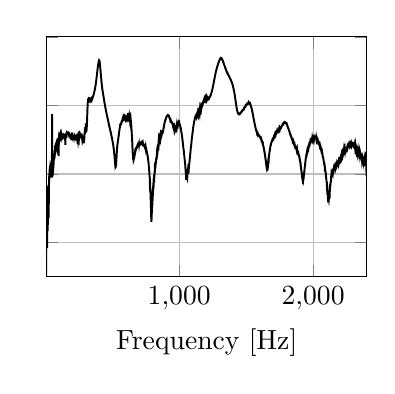
\begin{tikzpicture}

\begin{axis}[%
width=1.6in,
height=1.2in,
at={(1.011in,0.642in)},
scale only axis,
xmin=10,
xmax=2400,
xmajorgrids,
ymin=-30,
ymax=40,
ymajorgrids,
yticklabels={\empty},
xlabel={Frequency [Hz]},
axis background/.style={fill=white}
]
\addplot [color=black,solid,line width=0.7pt,forget plot]
  table[row sep=crcr]{%
0	-24.0538354294157\\
0.666675926054529	-24.7753265988161\\
1.33335185210906	-17.0382142167054\\
2.00002777816359	-18.7091958464009\\
2.66670370421811	-15.2032203403674\\
3.33337963027264	-8.53240216903954\\
4.00005555632717	-11.3881994991362\\
4.6667314823817	-7.34560264257265\\
5.33340740843623	-18.2635506378542\\
6.00008333449076	-30.0942089020284\\
6.66675926054529	-19.9100525240877\\
7.33343518659981	-21.3301429245582\\
8.00011111265434	-12.5504612701741\\
8.66678703870887	-15.3173206273707\\
9.3334629647634	-16.4624344447724\\
10.0001388908179	-21.0645945373479\\
10.6668148168725	-3.12818941832146\\
11.333490742927	-11.9814488880043\\
12.0001666689815	-16.3022691455521\\
12.666842595036	-16.83987041645\\
13.3335185210906	-21.5899394615097\\
14.0001944471451	-13.7669096045867\\
14.6668703731996	-10.7405701876275\\
15.3335462992542	-15.2513158642638\\
16.0002222253087	-12.4863764223308\\
16.6668981513632	-16.6735097060995\\
17.3335740774177	-11.1717261599997\\
18.0002500034723	-12.5642528883313\\
18.6669259295268	-14.7472480345922\\
19.3336018555813	-11.2309845901286\\
20.0002777816359	-12.3162845124428\\
20.6669537076904	-11.4989738149538\\
21.3336296337449	-11.4096075000397\\
22.0003055597994	-9.12000474667151\\
22.666981485854	-10.7058004870771\\
23.3336574119085	-10.8809274726073\\
24.000333337963	-12.8662435001899\\
24.6670092640176	-11.8084750036958\\
25.3336851900721	-9.39395341959846\\
26.0003611161266	-8.24921214045294\\
26.6670370421811	-5.13381010519183\\
27.3337129682357	-3.18474239145848\\
28.0003888942902	-1.96722097075604\\
28.6670648203447	-0.784435151267227\\
29.3337407463993	-0.564906469804107\\
30.0004166724538	-0.186628957762319\\
30.6670925985083	-0.223251397409185\\
31.3337685245628	-0.504288220825217\\
32.0004444506174	0.568981042424691\\
32.6671203766719	1.35135500831269\\
33.3337963027264	2.07752313968372\\
34.000472228781	2.13542686965292\\
34.6671481548355	1.87531635457994\\
35.33382408089	1.39408656672323\\
36.0005000069445	1.73767859557768\\
36.6671759329991	2.0365044287877\\
37.3338518590536	1.89103926658294\\
38.0005277851081	2.35267884483987\\
38.6672037111627	1.56785421692384\\
39.3338796372172	1.90575107773699\\
40.0005555632717	2.00696032260007\\
40.6672314893262	1.03747920044889\\
41.3339074153808	1.17819088709842\\
42.0005833414353	0.954423868100655\\
42.6672592674898	1.30215992319235\\
43.3339351935444	0.350798652357415\\
44.0006111195989	0.985446439692533\\
44.6672870456534	0.90853396189502\\
45.3339629717079	0.62363591607582\\
46.0006388977625	-0.106343649210524\\
46.667314823817	0.831296333741743\\
47.3339907498715	-0.154770617292899\\
48.0006666759261	-1.02488609973931\\
48.6673426019806	-0.349480793537451\\
49.3340185280351	1.40704941488586\\
50.0006944540896	17.4718617826514\\
50.6673703801442	-0.110905813330712\\
51.3340463061987	-0.969659382628823\\
52.0007222322532	-0.0156867446368573\\
52.6673981583078	-0.551828701230483\\
53.3340740843623	-0.335862030640212\\
54.0007500104168	-0.335709857720363\\
54.6674259364713	0.0689743844497208\\
55.3341018625259	0.149551305724914\\
56.0007777885804	0.650309261837628\\
56.6674537146349	0.13127845032964\\
57.3341296406895	0.572893104113807\\
58.000805566744	1.62672333434496\\
58.6674814927985	1.26340437511365\\
59.334157418853	1.80899399010958\\
60.0008333449076	2.12981393976939\\
60.6675092709621	2.11650037311116\\
61.3341851970166	2.70708359394901\\
62.0008611230712	3.0904031747816\\
62.6675370491257	3.73986090672288\\
63.3342129751802	4.11330532821165\\
64.0008889012347	4.28674048448287\\
64.6675648272893	4.49035790210038\\
65.3342407533438	4.62847704213878\\
66.0009166793983	4.90198327452499\\
66.6675926054529	5.40008752071958\\
67.3342685315074	5.71703775555609\\
68.0009444575619	5.85097210178158\\
68.6676203836164	6.35761681680145\\
69.334296309671	6.08420980880188\\
70.0009722357255	6.64342923814009\\
70.66764816178	7.14135937639171\\
71.3343240878346	6.95464466848458\\
72.0010000138891	7.3129468105897\\
72.6676759399436	7.26459405404091\\
73.3343518659981	7.48955717792348\\
74.0010277920527	7.65281470189807\\
74.6677037181072	7.55994571809288\\
75.3343796441617	7.89864326786307\\
76.0010555702163	7.63565632099739\\
76.6677314962708	7.89041771858883\\
77.3344074223253	7.83096423098779\\
78.0010833483798	7.95135021906428\\
78.6677592744344	8.15539545641694\\
79.3344352004889	8.08097874440249\\
80.0011111265434	8.18021272365017\\
80.667787052598	8.07561638981303\\
81.3344629786525	8.25782290136518\\
82.001138904707	8.02073159088786\\
82.6678148307615	8.42045087216576\\
83.3344907568161	8.1720438868478\\
84.0011666828706	8.11684485463587\\
84.6678426089251	8.2417824677993\\
85.3345185349797	8.26712476535566\\
86.0011944610342	8.08504729168952\\
86.6678703870887	8.39789867716215\\
87.3345463131432	8.45805928829301\\
88.0012222391978	8.62377756428815\\
88.6678981652523	8.52135557057066\\
89.3345740913068	8.67286525798598\\
90.0012500173614	8.85355762434988\\
90.6679259434159	9.00674645844902\\
91.3346018694704	9.00323229748388\\
92.0012777955249	9.23116144689982\\
92.6679537215795	9.19999321913624\\
93.334629647634	9.50702604628386\\
94.0013055736885	9.45354688509768\\
94.667981499743	9.60383675740148\\
95.3346574257976	9.70982758186113\\
96.0013333518521	9.81285612358788\\
96.6680092779066	9.87638222161103\\
97.3346852039612	9.98483507794277\\
98.0013611300157	10.2942179709114\\
98.6680370560702	10.0031320006568\\
99.3347129821248	10.234773264154\\
100.001388908179	5.20184010335849\\
100.668064834234	10.3673215378573\\
101.334740760288	10.6274246360448\\
102.001416686343	10.4963515327758\\
102.668092612397	10.6542180163706\\
103.334768538452	10.7270778119256\\
104.001444464506	10.7819900241968\\
104.668120390561	10.7476723911233\\
105.334796316616	10.8325568137231\\
106.00147224267	10.8565506329254\\
106.668148168725	10.7596885055515\\
107.334824094779	10.8153760411215\\
108.001500020834	10.9762515491244\\
108.668175946888	10.8813195235123\\
109.334851872943	10.9925472761605\\
110.001527798997	10.9839929711865\\
110.668203725052	10.8686273624886\\
111.334879651106	11.0336623311015\\
112.001555577161	10.8730227732298\\
112.668231503215	10.9764025968798\\
113.33490742927	10.9983924451575\\
114.001583355324	10.9932925852229\\
114.668259281379	10.8960860250767\\
115.334935207433	11.0971781560784\\
116.001611133488	10.9225306848365\\
116.668287059542	11.0012243151441\\
117.334962985597	10.9648906846422\\
118.001638911652	10.9810263450442\\
118.668314837706	10.9379766425556\\
119.334990763761	11.1180725359593\\
120.001666689815	10.8929973912361\\
120.66834261587	11.0346640034571\\
121.335018541924	11.0481488291843\\
122.001694467979	10.9418186978645\\
122.668370394033	10.9612899966686\\
123.335046320088	11.0949368089496\\
124.001722246142	11.0275110263947\\
124.668398172197	11.0715594833017\\
125.335074098251	11.0376539663672\\
126.001750024306	11.0892758690246\\
126.66842595036	10.9886866530624\\
127.335101876415	11.0544953488913\\
128.001777802469	11.086336614077\\
128.668453728524	11.0865827205247\\
129.335129654579	11.151384248337\\
130.001805580633	10.9699624040942\\
130.668481506688	11.0483383214513\\
131.335157432742	10.9434165920957\\
132.001833358797	10.9841995342106\\
132.668509284851	10.9498354463623\\
133.335185210906	11.0340101655261\\
134.00186113696	11.029981192541\\
134.668537063015	11.0002931400599\\
135.335212989069	11.0204717300212\\
136.001888915124	11.1082018634322\\
136.668564841178	11.1568604863805\\
137.335240767233	11.1212185688567\\
138.001916693287	11.1294445155704\\
138.668592619342	11.1038752994809\\
139.335268545396	10.9998777913079\\
140.001944471451	11.1203026571863\\
140.668620397506	11.0733110543624\\
141.33529632356	11.0783161713784\\
142.001972249615	11.2439397643653\\
142.668648175669	11.2245715123987\\
143.335324101724	11.2391735719326\\
144.002000027778	11.1714848438515\\
144.668675953833	11.2026579366728\\
145.335351879887	11.2800097757605\\
146.002027805942	11.2495634076332\\
146.668703731996	11.2875569503243\\
147.335379658051	11.2471604174122\\
148.002055584105	11.1433818238356\\
148.66873151016	11.1388023114834\\
149.335407436214	11.1083861020826\\
150.002083362269	8.49741873996997\\
150.668759288323	11.1444882241036\\
151.335435214378	11.0005689822991\\
152.002111140433	11.09039658558\\
152.668787066487	10.8554925363678\\
153.335462992542	10.8230173346571\\
154.002138918596	10.7685161320987\\
154.668814844651	10.8025435798439\\
155.335490770705	10.8135716851329\\
156.00216669676	10.8884190427297\\
156.668842622814	10.9438115197653\\
157.335518548869	11.108803501707\\
158.002194474923	11.3144993317585\\
158.668870400978	11.4290657039367\\
159.335546327032	11.5481305271641\\
160.002222253087	11.6743280140396\\
160.668898179141	11.5883742832391\\
161.335574105196	11.7607504814805\\
162.00225003125	11.7807862470171\\
162.668925957305	11.7467331034677\\
163.335601883359	11.7720285142441\\
164.002277809414	11.865060510984\\
164.668953735469	11.8803413440672\\
165.335629661523	11.8496811571761\\
166.002305587578	11.8324429598668\\
166.668981513632	11.8667775954332\\
167.335657439687	11.8685622372693\\
168.002333365741	11.9232402284661\\
168.669009291796	11.8631809517039\\
169.33568521785	11.8759285605512\\
170.002361143905	11.8500965787323\\
170.669037069959	11.8571411550248\\
171.335712996014	11.840672603201\\
172.002388922068	11.8726577669399\\
172.669064848123	11.8533596087701\\
173.335740774177	11.8970916548876\\
174.002416700232	11.8468821113692\\
174.669092626286	11.734120995521\\
175.335768552341	11.8545513954528\\
176.002444478396	11.8158272749587\\
176.66912040445	11.7581664010188\\
177.335796330505	11.6836690090809\\
178.002472256559	11.6134801753138\\
178.669148182614	11.545810162315\\
179.335824108668	11.580584591223\\
180.002500034723	11.4595817698421\\
180.669175960777	11.4109370365664\\
181.335851886832	11.4412280239627\\
182.002527812886	11.3337838862883\\
182.669203738941	11.2999958705124\\
183.335879664995	11.1766744105449\\
184.00255559105	11.2423046356787\\
184.669231517104	11.1506457429113\\
185.335907443159	11.049732946448\\
186.002583369213	11.0348385490678\\
186.669259295268	10.9294966777896\\
187.335935221323	10.9572626544397\\
188.002611147377	10.8441491005265\\
188.669287073432	10.7614007006402\\
189.335962999486	10.8383622788044\\
190.002638925541	10.8223907753729\\
190.669314851595	10.7318338151655\\
191.33599077765	10.7100341320297\\
192.002666703704	10.7954568913161\\
192.669342629759	10.7139401669828\\
193.336018555813	10.713553310691\\
194.002694481868	10.635326664087\\
194.669370407922	10.6914812192458\\
195.336046333977	10.6304543558945\\
196.002722260031	10.5135925535991\\
196.669398186086	10.4715652095356\\
197.33607411214	10.5958860446936\\
198.002750038195	10.5306409463711\\
198.66942596425	10.4646703088243\\
199.336101890304	10.6092591671541\\
200.002777816359	12.176381241264\\
200.669453742413	10.2229758071463\\
201.336129668468	10.4153000149645\\
202.002805594522	10.3409691366951\\
202.669481520577	10.3235299169775\\
203.336157446631	10.3908025729026\\
204.002833372686	10.4138955910993\\
204.66950929874	10.3096744183899\\
205.336185224795	10.3453530804593\\
206.002861150849	10.3411853460071\\
206.669537076904	10.4480086525697\\
207.336213002958	10.4821232768291\\
208.002888929013	10.4782237851814\\
208.669564855067	10.4857169071064\\
209.336240781122	10.5311820067122\\
210.002916707176	10.4065344665566\\
210.669592633231	10.3923410309562\\
211.336268559286	10.6125002075106\\
212.00294448534	10.6536877422631\\
212.669620411395	10.7075804710469\\
213.336296337449	10.5876450829407\\
214.002972263504	10.785798510488\\
214.669648189558	10.7575411253791\\
215.336324115613	10.8579433895683\\
216.003000041667	10.7564385534333\\
216.669675967722	10.8042910533961\\
217.336351893776	10.8590732035752\\
218.003027819831	10.9682998268144\\
218.669703745885	11.0298691531318\\
219.33637967194	10.9137424231625\\
220.003055597994	10.9268202865757\\
220.669731524049	11.1075459985888\\
221.336407450103	11.075272216335\\
222.003083376158	11.086723169469\\
222.669759302213	11.0306575287198\\
223.336435228267	11.0403269613152\\
224.003111154322	11.0461550610758\\
224.669787080376	10.8987251166676\\
225.336463006431	11.0093707380612\\
226.003138932485	11.0240270702722\\
226.66981485854	10.9899016358706\\
227.336490784594	10.8944098283972\\
228.003166710649	10.9776206027929\\
228.669842636703	10.9736768644323\\
229.336518562758	10.8881763913664\\
230.003194488812	10.8147798963354\\
230.669870414867	10.8177980422617\\
231.336546340921	10.8801157606152\\
232.003222266976	10.7283892320993\\
232.66989819303	10.6923124365478\\
233.336574119085	10.6786896011715\\
234.00325004514	10.4897476958619\\
234.669925971194	10.404416602913\\
235.336601897249	10.4085737009613\\
236.003277823303	10.3496630498464\\
236.669953749358	10.1939045392367\\
237.336629675412	10.3169473114109\\
238.003305601467	10.1109290157154\\
238.669981527521	10.0248242509185\\
239.336657453576	10.1248539008033\\
240.00333337963	9.86436784106379\\
240.670009305685	9.8461708563927\\
241.336685231739	9.80195907429479\\
242.003361157794	9.64681516121719\\
242.670037083848	9.65408983891004\\
243.336713009903	9.64755097355667\\
244.003388935957	9.47436381574311\\
244.670064862012	9.69859835886352\\
245.336740788066	9.54318354785978\\
246.003416714121	9.49157196217345\\
246.670092640176	9.61708331200281\\
247.33676856623	9.50254143555163\\
248.003444492285	9.58131774016605\\
248.670120418339	9.64528546865235\\
249.336796344394	9.58633365463329\\
250.003472270448	12.4050619191467\\
250.670148196503	10.1242217578109\\
251.336824122557	10.2671567123367\\
252.003500048612	10.562974536905\\
252.670175974666	10.6266234932955\\
253.336851900721	10.9711197026256\\
254.003527826775	10.9239309001141\\
254.67020375283	11.1999188615017\\
255.336879678884	11.1621178497936\\
256.003555604939	11.2330035027116\\
256.670231530993	11.3717480990161\\
257.336907457048	11.2397660539757\\
258.003583383103	11.3954434534165\\
258.670259309157	11.3330748055864\\
259.336935235212	11.4058114171549\\
260.003611161266	11.2727472424142\\
260.670287087321	11.3636069598555\\
261.336963013375	11.2803775781245\\
262.00363893943	11.3259731226633\\
262.670314865484	11.2831604198853\\
263.336990791539	11.2970077507477\\
264.003666717593	11.2537331196235\\
264.670342643648	11.2713568426248\\
265.337018569702	11.3038926896259\\
266.003694495757	11.1358976611144\\
266.670370421811	11.1288309856658\\
267.337046347866	11.0294360965846\\
268.00372227392	11.0311289283396\\
268.670398199975	11.0007018289668\\
269.33707412603	11.0526529539627\\
270.003750052084	10.9707716276467\\
270.670425978139	10.9747508530712\\
271.337101904193	10.6875614006601\\
272.003777830248	10.6611130565119\\
272.670453756302	10.5717850048715\\
273.337129682357	10.5648078472567\\
274.003805608411	10.499670336142\\
274.670481534466	10.3345037671487\\
275.33715746052	10.3743864040961\\
276.003833386575	10.0797133188244\\
276.670509312629	10.1874548657822\\
277.337185238684	9.99716266636554\\
278.003861164738	10.1329365143356\\
278.670537090793	9.9044650867058\\
279.337213016847	9.90190216469012\\
280.003888942902	9.79109249278751\\
280.670564868956	9.69492326926132\\
281.337240795011	9.69363522684118\\
282.003916721066	9.65539655977496\\
282.67059264712	9.61784377633952\\
283.337268573175	9.46150954678035\\
284.003944499229	9.4282426236971\\
284.670620425284	9.38794458809271\\
285.337296351338	9.3152770019253\\
286.003972277393	9.25769508223686\\
286.670648203447	9.19487404101757\\
287.337324129502	9.19501777667553\\
288.004000055556	9.35798780902652\\
288.670675981611	9.49456436606766\\
289.337351907665	9.7814876541983\\
290.00402783372	9.98147689201293\\
290.670703759774	10.2208175989873\\
291.337379685829	10.7311048602494\\
292.004055611883	11.0344757195201\\
292.670731537938	11.5192982400905\\
293.337407463993	11.8743752751125\\
294.004083390047	12.193556622589\\
294.670759316102	12.5652111611462\\
295.337435242156	12.9287677400434\\
296.004111168211	13.1378622004779\\
296.670787094265	13.2747682449318\\
297.33746302032	13.4282695085721\\
298.004138946374	13.5102474369325\\
298.670814872429	13.5312473320591\\
299.337490798483	13.3928499746803\\
300.004166724538	12.9948684163598\\
300.670842650592	13.3480927038971\\
301.337518576647	13.2475020503163\\
302.004194502701	13.0146629162693\\
302.670870428756	12.9962216245747\\
303.33754635481	12.8169344827781\\
304.004222280865	12.6361683472883\\
304.67089820692	12.5235804864241\\
305.337574132974	12.5701827364406\\
306.004250059029	12.4868789069686\\
306.670925985083	12.52032409134\\
307.337601911138	12.6466781948824\\
308.004277837192	12.9524182617077\\
308.670953763247	13.1715673652573\\
309.337629689301	13.5704043890882\\
310.004305615356	14.1606552716047\\
310.67098154141	14.7443826657853\\
311.337657467465	15.338294799873\\
312.004333393519	16.1663799368635\\
312.671009319574	16.9192556224687\\
313.337685245628	17.6011943590241\\
314.004361171683	18.3488092168469\\
314.671037097737	19.0888640542677\\
315.337713023792	19.6139738831932\\
316.004388949847	20.137762039088\\
316.671064875901	20.6552163789144\\
317.337740801956	20.9438530908394\\
318.00441672801	21.2412621975858\\
318.671092654065	21.4919486764409\\
319.337768580119	21.5977339205972\\
320.004444506174	21.7344452957731\\
320.671120432228	21.8822169758041\\
321.337796358283	21.9017537206537\\
322.004472284337	21.9473771938291\\
322.671148210392	22.0123528794745\\
323.337824136446	21.9793451486636\\
324.004500062501	22.0386109699524\\
324.671175988555	22.0408994279567\\
325.33785191461	21.9463862242842\\
326.004527840664	21.9753419819211\\
326.671203766719	21.933473132491\\
327.337879692774	21.875025790672\\
328.004555618828	21.8993855851231\\
328.671231544883	21.8122241818433\\
329.337907470937	21.7672598455656\\
330.004583396992	21.732754647684\\
330.671259323046	21.6567658373683\\
331.337935249101	21.6943787143949\\
332.004611175155	21.6311949762639\\
332.67128710121	21.5903275519017\\
333.337963027264	21.6334126166854\\
334.004638953319	21.4963114789822\\
334.671314879373	21.5484005574098\\
335.337990805428	21.5199247030615\\
336.004666731482	21.4870156650135\\
336.671342657537	21.544078906322\\
337.338018583591	21.4763389952504\\
338.004694509646	21.5451236206611\\
338.671370435701	21.5002992156288\\
339.338046361755	21.4914266245329\\
340.00472228781	21.5414916462764\\
340.671398213864	21.4969145634654\\
341.338074139919	21.5806730359757\\
342.004750065973	21.5164955323163\\
342.671425992028	21.631180114211\\
343.338101918082	21.6280672198441\\
344.004777844137	21.6524481284436\\
344.671453770191	21.6925161231834\\
345.338129696246	21.684657990614\\
346.0048056223	21.7959021361112\\
346.671481548355	21.7503780623695\\
347.338157474409	21.8858944759259\\
348.004833400464	21.8359367974069\\
348.671509326518	21.9503421196585\\
349.338185252573	21.9392384364729\\
350.004861178627	22.3870856318804\\
350.671537104682	22.0939943700624\\
351.338213030737	22.1333651372974\\
352.004888956791	22.1859159985505\\
352.671564882846	22.2314050905983\\
353.3382408089	22.3277504526568\\
354.004916734955	22.3332928147098\\
354.671592661009	22.456914580025\\
355.338268587064	22.5116795513418\\
356.004944513118	22.6268407556826\\
356.671620439173	22.6579767266709\\
357.338296365227	22.7830279539719\\
358.004972291282	22.7855363418947\\
358.671648217336	22.9282977061801\\
359.338324143391	22.9552004342005\\
360.005000069445	23.0967482034254\\
360.6716759955	23.1375534974305\\
361.338351921554	23.2671336898219\\
362.005027847609	23.3418111710958\\
362.671703773664	23.4712828577667\\
363.338379699718	23.553824857098\\
364.005055625773	23.6818063134887\\
364.671731551827	23.7736665359105\\
365.338407477882	23.8530357605844\\
366.005083403936	23.9997124292131\\
366.671759329991	24.0838168121703\\
367.338435256045	24.2347500113039\\
368.0051111821	24.3173935102669\\
368.671787108154	24.4909965246874\\
369.338463034209	24.558499138546\\
370.005138960263	24.7636680115791\\
370.671814886318	24.8500775519553\\
371.338490812372	25.0340991190821\\
372.005166738427	25.1554181253712\\
372.671842664481	25.31138732569\\
373.338518590536	25.503138701614\\
374.005194516591	25.5945440661062\\
374.671870442645	25.8258923739692\\
375.3385463687	25.8781832785756\\
376.005222294754	26.1212069673736\\
376.671898220809	26.2359863801086\\
377.338574146863	26.4563924416597\\
378.005250072918	26.6378861199214\\
378.671925998972	26.8034489554332\\
379.338601925027	27.0717627153897\\
380.005277851081	27.212045496638\\
380.671953777136	27.4561675539983\\
381.33862970319	27.6365587895402\\
382.005305629245	27.8153213652563\\
382.671981555299	28.0774413338392\\
383.338657481354	28.2342218562877\\
384.005333407408	28.5087659524338\\
384.672009333463	28.7540223326795\\
385.338685259517	28.9316679728972\\
386.005361185572	29.2350413994742\\
386.672037111627	29.3966621511991\\
387.338713037681	29.641209895069\\
388.005388963736	29.9193384375346\\
388.67206488979	30.0889819929086\\
389.338740815845	30.3889089301848\\
390.005416741899	30.5834284748198\\
390.672092667954	30.7520419489202\\
391.338768594008	31.0253306189734\\
392.005444520063	31.1691438622083\\
392.672120446117	31.3805029492705\\
393.338796372172	31.6109791175107\\
394.005472298226	31.7088394068235\\
394.672148224281	31.8977166816165\\
395.338824150335	32.118590197554\\
396.00550007639	32.2250301442221\\
396.672176002444	32.4383969709178\\
397.338851928499	32.584372014053\\
398.005527854554	32.652834316717\\
398.672203780608	32.8554270618435\\
399.338879706663	32.9949422192336\\
400.005555632717	33.0478065427637\\
400.672231558772	33.1054097052581\\
401.338907484826	33.2000438623887\\
402.005583410881	33.1679382029102\\
402.672259336935	33.1553109660612\\
403.33893526299	33.148151872368\\
404.005611189044	33.0332835311622\\
404.672287115099	32.9205788736783\\
405.338963041153	32.810301879351\\
406.005638967208	32.5985487610059\\
406.672314893262	32.3851116469242\\
407.338990819317	32.2026022497992\\
408.005666745371	31.9559744308648\\
408.672342671426	31.6418704159758\\
409.339018597481	31.3864409761776\\
410.005694523535	31.1469497092695\\
410.67237044959	30.7977082329506\\
411.339046375644	30.4783875394015\\
412.005722301699	30.2433520025839\\
412.672398227753	29.9082916554792\\
413.339074153808	29.5561508893066\\
414.005750079862	29.2914123673672\\
414.672426005917	29.0006488166639\\
415.339101931971	28.6876653242218\\
416.005777858026	28.3640825702083\\
416.67245378408	28.0606596600821\\
417.339129710135	27.8503313282515\\
418.005805636189	27.5189732830465\\
418.672481562244	27.1808685798042\\
419.339157488298	26.9525030135891\\
420.005833414353	26.7409332472361\\
420.672509340407	26.4505140133333\\
421.339185266462	26.1373778956874\\
422.005861192517	25.9445242047876\\
422.672537118571	25.7238560344385\\
423.339213044626	25.5265166116736\\
424.00588897068	25.2491125724447\\
424.672564896735	25.0250081623613\\
425.339240822789	24.8974975226114\\
426.005916748844	24.7224643389561\\
426.672592674898	24.5006868441122\\
427.339268600953	24.3066994958521\\
428.005944527007	24.1462413550494\\
428.672620453062	24.0507375112873\\
429.339296379116	23.8892840468726\\
430.005972305171	23.6776851026303\\
430.672648231225	23.5099653059884\\
431.33932415728	23.3478236259535\\
432.006000083334	23.2364127595894\\
432.672676009389	23.1207612587907\\
433.339351935444	22.8959361913742\\
434.006027861498	22.7471931522182\\
434.672703787553	22.5433582405117\\
435.339379713607	22.4547303842041\\
436.006055639662	22.2914653457661\\
436.672731565716	22.1519722574286\\
437.339407491771	21.9399191349777\\
438.006083417825	21.7290116106934\\
438.67275934388	21.5988691511031\\
439.339435269934	21.4594341238752\\
440.006111195989	21.3562168861861\\
440.672787122043	21.144900900334\\
441.339463048098	20.9739586695309\\
442.006138974152	20.7736080862848\\
442.672814900207	20.6201277638556\\
443.339490826261	20.5023998974435\\
444.006166752316	20.389707420288\\
444.672842678371	20.2221190500421\\
445.339518604425	20.1150004192628\\
446.00619453048	19.8958868027358\\
446.672870456534	19.7185496925901\\
447.339546382589	19.5946554813454\\
448.006222308643	19.4447782425543\\
448.672898234698	19.3248187746355\\
449.339574160752	19.2415878026817\\
450.006250086807	19.1969702927045\\
450.672926012861	18.9235712221156\\
451.339601938916	18.786476495092\\
452.00627786497	18.6138438464368\\
452.672953791025	18.458029742538\\
453.339629717079	18.3735391635682\\
454.006305643134	18.2274483277047\\
454.672981569188	18.1198667818157\\
455.339657495243	17.9970599081178\\
456.006333421298	17.9104914480584\\
456.673009347352	17.7908964404868\\
457.339685273407	17.6300876671202\\
458.006361199461	17.5205393224243\\
458.673037125516	17.3789005038587\\
459.33971305157	17.219497155265\\
460.006388977625	17.0916857427261\\
460.673064903679	16.967776133388\\
461.339740829734	16.8481704528801\\
462.006416755788	16.7606037216756\\
462.673092681843	16.6287300042932\\
463.339768607897	16.5150807513815\\
464.006444533952	16.4335668264479\\
464.673120460006	16.3541986927064\\
465.339796386061	16.2444898512573\\
466.006472312115	16.1022276577805\\
466.67314823817	16.0099998689133\\
467.339824164225	15.8321201445416\\
468.006500090279	15.731463989389\\
468.673176016334	15.598667407565\\
469.339851942388	15.4434925118285\\
470.006527868443	15.3418255048297\\
470.673203794497	15.260400829156\\
471.339879720552	15.1028294124931\\
472.006555646606	14.9703269586253\\
472.673231572661	14.8720922816024\\
473.339907498715	14.7048017505083\\
474.00658342477	14.6348712133549\\
474.673259350824	14.5046704313732\\
475.339935276879	14.3409902316396\\
476.006611202933	14.2909428993713\\
476.673287128988	14.1090275349316\\
477.339963055042	13.9893366679867\\
478.006638981097	13.9396784257778\\
478.673314907152	13.8030625702837\\
479.339990833206	13.6464528292807\\
480.006666759261	13.6262442302645\\
480.673342685315	13.4337902085009\\
481.34001861137	13.2908180780304\\
482.006694537424	13.2238446919687\\
482.673370463479	13.1087385153536\\
483.340046389533	12.9774902252141\\
484.006722315588	12.9235558923937\\
484.673398241642	12.7797322506448\\
485.340074167697	12.6652555108802\\
486.006750093751	12.5296361654673\\
486.673426019806	12.4705219488855\\
487.34010194586	12.3409420524972\\
488.006777871915	12.1918314613151\\
488.673453797969	12.1237800371845\\
489.340129724024	12.1137693010676\\
490.006805650078	11.9399408447004\\
490.673481576133	11.7769438523611\\
491.340157502188	11.6521991299404\\
492.006833428242	11.5335559889926\\
492.673509354297	11.3711021779641\\
493.340185280351	11.2797519092352\\
494.006861206406	11.1450543787188\\
494.67353713246	11.0490224157538\\
495.340213058515	10.8802703470087\\
496.006888984569	10.6657933239491\\
496.673564910624	10.639583194267\\
497.340240836678	10.5331311702954\\
498.006916762733	10.4376658346226\\
498.673592688787	10.226261189877\\
499.340268614842	10.173280789518\\
500.006944540896	9.97658207157796\\
500.673620466951	9.93104255542565\\
501.340296393005	9.70299151470093\\
502.00697231906	9.56427842467682\\
502.673648245115	9.40966460679045\\
503.340324171169	9.23208529134278\\
504.007000097224	9.16591247293168\\
504.673676023278	9.02470332922051\\
505.340351949333	8.85799847535677\\
506.007027875387	8.68232112750533\\
506.673703801442	8.49015542367151\\
507.340379727496	8.35612313467402\\
508.007055653551	8.09827396310981\\
508.673731579605	7.95619332879397\\
509.34040750566	7.71668486249847\\
510.007083431714	7.54408425757578\\
510.673759357769	7.3866368832407\\
511.340435283823	7.20454326168255\\
512.007111209878	6.96606098465922\\
512.673787135932	6.72619901342163\\
513.340463061987	6.33214482749454\\
514.007138988041	6.09664452506388\\
514.673814914096	6.00821140207314\\
515.340490840151	5.68996033058963\\
516.007166766205	5.41891292066807\\
516.67384269226	5.19913029101021\\
517.340518618314	4.74641232196898\\
518.007194544369	4.44353283286356\\
518.673870470423	4.18881886188834\\
519.340546396478	3.84761742946598\\
520.007222322532	3.53418988119992\\
520.673898248587	3.14939886494411\\
521.340574174641	2.838292842742\\
522.007250100696	2.57379153395263\\
522.67392602675	2.68621460723454\\
523.340601952805	2.54268561550195\\
524.007277878859	2.44119387057222\\
524.673953804914	2.34546990210759\\
525.340629730968	2.12788718992\\
526.007305657023	2.17247785298671\\
526.673981583078	2.17437754975731\\
527.340657509132	2.30955463293454\\
528.007333435187	2.32552210191851\\
528.674009361241	2.56150916661386\\
529.340685287296	3.1056710717391\\
530.00736121335	3.77675628169621\\
530.674037139405	4.23542156703512\\
531.340713065459	4.5715970853357\\
532.007388991514	4.98174110027376\\
532.674064917568	5.72223246797755\\
533.340740843623	6.01634248893307\\
534.007416769677	6.40373719646523\\
534.674092695732	6.81682238561117\\
535.340768621786	7.17875928125927\\
536.007444547841	7.47873462105253\\
536.674120473896	7.80929354526687\\
537.34079639995	8.05245706986005\\
538.007472326005	8.36022547474432\\
538.674148252059	8.58557421707928\\
539.340824178114	8.81462764879022\\
540.007500104168	8.93724767281927\\
540.674176030223	9.30767053508195\\
541.340851956277	9.41314167146452\\
542.007527882332	9.55514198421905\\
542.674203808386	9.80504696603795\\
543.340879734441	10.0715779624224\\
544.007555660495	10.1903989708205\\
544.67423158655	10.3261730853789\\
545.340907512604	10.5231373859331\\
546.007583438659	10.7373606145697\\
546.674259364713	10.8528441788335\\
547.340935290768	11.0243072468929\\
548.007611216823	11.3312786158819\\
548.674287142877	11.3774764740178\\
549.340963068932	11.6524856563262\\
550.007638994986	11.8209336106523\\
550.674314921041	12.0719428085404\\
551.340990847095	12.174427441001\\
552.00766677315	12.4054022511678\\
552.674342699204	12.675640934017\\
553.341018625259	12.8103604363372\\
554.007694551313	12.9886014144124\\
554.674370477368	13.1767125315813\\
555.341046403422	13.3030478639295\\
556.007722329477	13.4715164884348\\
556.674398255531	13.7083858707781\\
557.341074181586	13.7995387628935\\
558.00775010764	13.9282687496593\\
558.674426033695	14.2224926371625\\
559.341101959749	14.2258110595647\\
560.007777885804	14.3252407459023\\
560.674453811858	14.5106403874977\\
561.341129737913	14.5096064949592\\
562.007805663968	14.5862548783372\\
562.674481590022	14.6686389667934\\
563.341157516077	14.668275787313\\
564.007833442131	14.7581885840426\\
564.674509368186	14.7889406640586\\
565.34118529424	14.7330637771831\\
566.007861220295	14.7761720485605\\
566.674537146349	14.7950379349273\\
567.341213072404	14.8136528998632\\
568.007888998458	14.9307479037634\\
568.674564924513	14.8869093992123\\
569.341240850567	15.0020057804691\\
570.007916776622	15.0448899036403\\
570.674592702676	15.0733428753757\\
571.341268628731	15.2653123767828\\
572.007944554785	15.2859544262324\\
572.67462048084	15.3244107965716\\
573.341296406895	15.5056585597125\\
574.007972332949	15.5463222031134\\
574.674648259004	15.7091986008417\\
575.341324185058	15.7857704631097\\
576.008000111113	15.8942386542656\\
576.674676037167	16.0257081173392\\
577.341351963222	16.0149498355079\\
578.008027889276	16.1879588740618\\
578.674703815331	16.1729269420844\\
579.341379741385	16.3083726802466\\
580.00805566744	16.3575588369278\\
580.674731593494	16.365937703832\\
581.341407519549	16.4928648069782\\
582.008083445603	16.4135098039103\\
582.674759371658	16.5606232989547\\
583.341435297712	16.4949869606825\\
584.008111223767	16.5875942777116\\
584.674787149822	16.5514655794609\\
585.341463075876	16.5654555789107\\
586.008139001931	16.6053193123706\\
586.674814927985	16.5052009636011\\
587.34149085404	16.6072309414191\\
588.008166780094	16.4786187578352\\
588.674842706149	16.5574939792168\\
589.341518632203	16.4367798218283\\
590.008194558258	16.4995798511669\\
590.674870484312	16.3865012367849\\
591.341546410367	16.4592085148972\\
592.008222336421	16.340487948373\\
592.674898262476	16.3670572759151\\
593.34157418853	16.3063615038774\\
594.008250114585	16.3455728584197\\
594.674926040639	16.2608916229011\\
595.341601966694	16.297350941732\\
596.008277892749	16.2025084546167\\
596.674953818803	16.2378002755367\\
597.341629744858	16.1963992046452\\
598.008305670912	16.1688825705917\\
598.674981596967	16.1131426357601\\
599.341657523021	16.2063396706033\\
600.008333449076	16.082470288651\\
600.67500937513	16.1749020334652\\
601.341685301185	16.1246008212953\\
602.008361227239	16.1984115744638\\
602.675037153294	16.0948019285334\\
603.341713079348	16.2170131537778\\
604.008389005403	16.1304315172695\\
604.675064931457	16.2492579274956\\
605.341740857512	16.1712036728509\\
606.008416783566	16.2362173440111\\
606.675092709621	16.2120105909438\\
607.341768635676	16.3022758438576\\
608.00844456173	16.2397755587875\\
608.675120487785	16.3371921941228\\
609.341796413839	16.3336724777239\\
610.008472339894	16.3313353363035\\
610.675148265948	16.3979196428623\\
611.341824192003	16.3129768461316\\
612.008500118057	16.4385269611059\\
612.675176044112	16.3194257948107\\
613.341851970166	16.4457013711349\\
614.008527896221	16.4065585931307\\
614.675203822275	16.4363597931761\\
615.34187974833	16.507449764277\\
616.008555674384	16.4506796275132\\
616.675231600439	16.5520510315926\\
617.341907526493	16.4627257345375\\
618.008583452548	16.624553047341\\
618.675259378603	16.5335960648416\\
619.341935304657	16.5616368108617\\
620.008611230711	16.636736390542\\
620.675287156766	16.5478634227533\\
621.341963082821	16.6756072286469\\
622.008639008875	16.5836004908967\\
622.67531493493	16.6108910965367\\
623.341990860984	16.6894703602389\\
624.008666787039	16.5677177530767\\
624.675342713093	16.6913117157591\\
625.342018639148	16.6488815610008\\
626.008694565202	16.5487677436973\\
626.675370491257	16.7555897507216\\
627.342046417311	16.55274074888\\
628.008722343366	16.5611432576366\\
628.67539826942	16.6416552804713\\
629.342074195475	16.4320030957751\\
630.008750121529	16.5406189712251\\
630.675426047584	16.580535623175\\
631.342101973638	16.267797586175\\
632.008777899693	16.4726226747189\\
632.675453825748	16.4025795355512\\
633.342129751802	16.1751980714638\\
634.008805677857	16.2920847485297\\
634.675481603911	16.0718224148971\\
635.342157529966	15.9247024759311\\
636.00883345602	16.0239536112237\\
636.675509382075	15.799687708656\\
637.342185308129	15.4575806981259\\
638.008861234184	15.6327066208098\\
638.675537160238	15.3118732652641\\
639.342213086293	14.8517393760472\\
640.008889012347	14.9662407330703\\
640.675564938402	14.7259462068026\\
641.342240864456	14.1296834286275\\
642.008916790511	13.9712980107766\\
642.675592716565	13.9101024775435\\
643.34226864262	13.1266704172734\\
644.008944568675	12.8538851703094\\
644.675620494729	12.7481594386484\\
645.342296420784	11.9965695483298\\
646.008972346838	11.4499069847361\\
646.675648272893	11.2990796911129\\
647.342324198947	10.7009231507117\\
648.009000125002	9.88953406030728\\
648.675676051056	9.50168700273076\\
649.342351977111	9.10954130375459\\
650.009027903165	8.64820776820932\\
650.67570382922	7.61756872242853\\
651.342379755274	7.40586741417076\\
652.009055681329	7.08942540282487\\
652.675731607383	6.08200626385361\\
653.342407533438	5.72419650143808\\
654.009083459492	5.49759242816381\\
654.675759385547	5.29169501571504\\
655.342435311602	4.71109730366877\\
656.009111237656	4.29505478873706\\
656.675787163711	4.61234146286363\\
657.342463089765	4.51977411033579\\
658.00913901582	4.24545086492994\\
658.675814941874	3.99616888525082\\
659.342490867929	4.07913016147592\\
660.009166793983	4.43900944385735\\
660.675842720038	4.38012170617682\\
661.342518646092	4.4514484809695\\
662.009194572147	4.55053847636848\\
662.675870498201	4.68581788631672\\
663.342546424256	5.06836396711243\\
664.00922235031	5.03834687003778\\
664.675898276365	5.01798182971722\\
665.342574202419	5.29255886284392\\
666.009250128474	5.57963088869587\\
666.675926054529	5.70082816841368\\
667.342601980583	5.66047564216475\\
668.009277906638	5.65110414379459\\
668.675953832692	6.05820324551451\\
669.342629758747	6.26256346656145\\
670.009305684801	6.18875699485358\\
670.675981610856	6.26566083216555\\
671.34265753691	6.37375958455085\\
672.009333462965	6.46899287385204\\
672.676009389019	6.7023481501977\\
673.342685315074	6.92994514722064\\
674.009361241128	6.9142441838001\\
674.676037167183	6.84390413844429\\
675.342713093237	6.93362228437308\\
676.009389019292	7.16013982468008\\
676.676064945346	7.29782724821155\\
677.342740871401	7.28099887468422\\
678.009416797456	7.28553560396656\\
678.67609272351	7.3438589447758\\
679.342768649565	7.35268456383873\\
680.009444575619	7.46013201228345\\
680.676120501674	7.58787823875755\\
681.342796427728	7.70987056832242\\
682.009472353783	7.7047698036689\\
682.676148279837	7.71836181754712\\
683.342824205892	7.71287810866602\\
684.009500131946	7.88491955520567\\
684.676176058001	7.88200458566801\\
685.342851984055	7.97871547719071\\
686.00952791011	8.06262035838028\\
686.676203836164	8.19454833038218\\
687.342879762219	8.16680871449154\\
688.009555688273	8.14986629672043\\
688.676231614328	8.11098997869995\\
689.342907540382	8.15600053376475\\
690.009583466437	8.2431174413041\\
690.676259392492	8.35857584547801\\
691.342935318546	8.47980551964391\\
692.009611244601	8.43020986419829\\
692.676287170655	8.48780149220811\\
693.34296309671	8.49475492350756\\
694.009639022764	8.48315887279011\\
694.676314948819	8.50345618383611\\
695.342990874873	8.48156685248925\\
696.009666800928	8.6273150299049\\
696.676342726982	8.65591179059107\\
697.343018653037	8.66517613107\\
698.009694579091	8.77821021920323\\
698.676370505146	8.75333557717898\\
699.3430464312	8.8738621831423\\
700.009722357255	8.65908011082201\\
700.676398283309	8.86688296460674\\
701.343074209364	8.99292078768806\\
702.009750135419	8.92702794124702\\
702.676426061473	8.94314707926746\\
703.343101987528	9.00448341199101\\
704.009777913582	8.99974507269237\\
704.676453839637	8.94855984341114\\
705.343129765691	8.91491375340969\\
706.009805691746	9.04507061596649\\
706.6764816178	9.03253887450496\\
707.343157543855	9.0075023601351\\
708.009833469909	8.99718959363287\\
708.676509395964	9.10477017565572\\
709.343185322018	9.17907052885568\\
710.009861248073	9.18639911781509\\
710.676537174127	9.08239240901507\\
711.343213100182	9.16189627843021\\
712.009889026236	9.19475262476087\\
712.676564952291	9.2117120724423\\
713.343240878346	9.24617414557119\\
714.0099168044	9.28100228694381\\
714.676592730455	9.3022214295608\\
715.343268656509	9.21367630460709\\
716.009944582564	9.22161749744294\\
716.676620508618	9.20051200364815\\
717.343296434673	9.19917213365312\\
718.009972360727	9.20628728333848\\
718.676648286782	9.15288523255609\\
719.343324212836	9.18144019305628\\
720.010000138891	9.0888488044096\\
720.676676064945	9.13366907544728\\
721.343351991	9.09691399403723\\
722.010027917054	9.07780768358352\\
722.676703843109	8.99477464928745\\
723.343379769163	9.06415786331838\\
724.010055695218	8.9396147449063\\
724.676731621273	8.91679571829932\\
725.343407547327	8.89078643803618\\
726.010083473382	8.89081486731126\\
726.676759399436	8.86587058208948\\
727.343435325491	8.82387149713632\\
728.010111251545	8.84742213310955\\
728.6767871776	8.80797109096137\\
729.343463103654	8.77921127750227\\
730.010139029709	8.88600239733476\\
730.676814955763	8.76052369591128\\
731.343490881818	8.84503878959984\\
732.010166807872	8.78348576588829\\
732.676842733927	8.74729278566041\\
733.343518659981	8.69718510731511\\
734.010194586036	8.58765820005153\\
734.67687051209	8.55866789218656\\
735.343546438145	8.57966892515378\\
736.0102223642	8.51429485733572\\
736.676898290254	8.47576228049317\\
737.343574216309	8.47350178943034\\
738.010250142363	8.36534874926045\\
738.676926068418	8.3134314464271\\
739.343601994472	8.30784562333557\\
740.010277920527	8.30356706532026\\
740.676953846581	8.29810828413785\\
741.343629772636	8.28230145879134\\
742.01030569869	8.19757323542451\\
742.676981624745	8.16306820019938\\
743.343657550799	8.10197498872195\\
744.010333476854	7.91140718178206\\
744.677009402908	7.95146581159202\\
745.343685328963	7.89349505820059\\
746.010361255017	7.81561049766296\\
746.677037181072	7.91101046118437\\
747.343713107127	7.81549474148716\\
748.010389033181	7.79004878356179\\
748.677064959236	7.66829467356041\\
749.34374088529	7.49522738347616\\
750.010416811345	7.68306725636067\\
750.677092737399	7.47542347743726\\
751.343768663454	7.30539756747948\\
752.010444589508	7.32444285285847\\
752.677120515563	7.19256018569224\\
753.343796441617	7.22101513454485\\
754.010472367672	6.98367788213361\\
754.677148293726	6.94151082884162\\
755.343824219781	6.81920124364684\\
756.010500145835	6.85561208875995\\
756.67717607189	6.73901309068327\\
757.343851997944	6.65447059917736\\
758.010527923999	6.39940819849267\\
758.677203850054	6.31537062804607\\
759.343879776108	6.2304774693665\\
760.010555702162	6.15132302820454\\
760.677231628217	6.03645142947089\\
761.343907554272	5.82856391160883\\
762.010583480326	5.62639500122763\\
762.677259406381	5.49140195078828\\
763.343935332435	5.29501650067733\\
764.01061125849	5.28840291402563\\
764.677287184544	5.13659478264419\\
765.343963110599	4.92696956390757\\
766.010639036653	4.65854266888813\\
766.677314962708	4.49329801241826\\
767.343990888762	4.39946911523809\\
768.010666814817	4.1882380007889\\
768.677342740871	3.83121132007652\\
769.344018666926	3.6747490934063\\
770.01069459298	3.51415478445073\\
770.677370519035	3.36285311572927\\
771.344046445089	2.99118916014252\\
772.010722371144	2.83533387759084\\
772.677398297199	2.31556653261333\\
773.344074223253	2.18825393175463\\
774.010750149308	1.94755390900186\\
774.677426075362	1.30582271184568\\
775.344102001417	1.12798424630628\\
776.010777927471	1.11609012507506\\
776.677453853526	0.541390822703892\\
777.34412977958	0.158386409686359\\
778.010805705635	-0.468980051040267\\
778.677481631689	-0.714193168197218\\
779.344157557744	-0.899055137537588\\
780.010833483798	-1.07703919157975\\
780.677509409853	-2.49646867206346\\
781.344185335907	-2.37501600216951\\
782.010861261962	-2.17316165963422\\
782.677537188016	-4.0581005908558\\
783.344213114071	-4.58062890864723\\
784.010889040126	-4.58269787118991\\
784.67756496618	-4.7208140869024\\
785.344240892235	-5.73279953533563\\
786.010916818289	-6.89575411330063\\
786.677592744344	-6.68381994855648\\
787.344268670398	-8.18517020034133\\
788.010944596453	-9.90652762988221\\
788.677620522507	-8.18289582525946\\
789.344296448562	-10.1846467980253\\
790.010972374616	-12.5734242530755\\
790.677648300671	-11.2925063282194\\
791.344324226725	-11.0326681826804\\
792.01100015278	-13.9522799585502\\
792.677676078834	-10.6894138613858\\
793.344352004889	-11.2152910111612\\
794.011027930943	-13.2516412128331\\
794.677703856998	-9.79569996931918\\
795.344379783053	-11.3022395543273\\
796.011055709107	-11.4952272503209\\
796.677731635162	-8.41722339018986\\
797.344407561216	-9.72627220711398\\
798.011083487271	-9.94979243639554\\
798.677759413325	-6.87502790192122\\
799.34443533938	-9.12375254882056\\
800.011111265434	-7.32160601680179\\
800.677787191489	-5.43797021337587\\
801.344463117543	-7.80256595429727\\
802.011139043598	-5.13409187346906\\
802.677814969652	-4.94108863994887\\
803.344490895707	-6.37745787416539\\
804.011166821761	-3.55950243852837\\
804.677842747816	-4.30586109253226\\
805.34451867387	-4.59397551263602\\
806.011194599925	-2.73093805028424\\
806.67787052598	-4.50721520541811\\
807.344546452034	-2.71904955651304\\
808.011222378089	-2.56406630580553\\
808.677898304143	-3.79276753181882\\
809.344574230198	-1.43233406110157\\
810.011250156252	-2.40888422001714\\
810.677926082307	-2.26245578595983\\
811.344602008361	-1.04421395839191\\
812.011277934416	-2.49516241499997\\
812.67795386047	-0.268917971359419\\
813.344629786525	-1.44027205880575\\
814.011305712579	-0.58017509754626\\
814.677981638634	-0.106411658385477\\
815.344657564688	-0.604591426118682\\
816.011333490743	0.94649791000057\\
816.678009416797	-0.0135856302018601\\
817.344685342852	1.01227256578035\\
818.011361268907	0.874174188656179\\
818.678037194961	1.14296528929029\\
819.344713121016	1.83339816048708\\
820.01138904707	1.37241871192462\\
820.678064973125	2.35754556263054\\
821.344740899179	1.695533751534\\
822.011416825234	2.65437077751505\\
822.678092751288	2.33195299209198\\
823.344768677343	2.6712027563085\\
824.011444603397	3.12226968652874\\
824.678120529452	2.85017726099925\\
825.344796455506	3.68194181903176\\
826.011472381561	3.10750420962551\\
826.678148307615	4.10803459146397\\
827.34482423367	3.63804406996872\\
828.011500159724	4.50743894422469\\
828.678176085779	4.26625290414105\\
829.344852011833	4.5765990683043\\
830.011527937888	4.72375359303579\\
830.678203863943	4.97318854745414\\
831.344879789997	5.04487623377831\\
832.011555716052	5.21440337067422\\
832.678231642106	5.4887612967534\\
833.344907568161	5.62068819776284\\
834.011583494215	6.0910417712059\\
834.67825942027	5.98735626527823\\
835.344935346324	6.328626218188\\
836.011611272379	6.43646375962649\\
836.678287198433	6.7736958348463\\
837.344963124488	6.82165695424229\\
838.011639050542	7.19372361307892\\
838.678314976597	7.11523922481778\\
839.344990902651	7.57138139653562\\
840.011666828706	7.557247900819\\
840.67834275476	7.90611873433456\\
841.345018680815	7.91608176675178\\
842.01169460687	8.09851421262908\\
842.678370532924	8.3536357220389\\
843.345046458979	8.40510316993884\\
844.011722385033	8.67827879791309\\
844.678398311088	8.72842127719789\\
845.345074237142	9.06145967026124\\
846.011750163197	8.85824675407166\\
846.678426089251	9.33381122591847\\
847.345102015306	9.16247240374297\\
848.01177794136	9.53714993615979\\
848.678453867415	9.45222110064775\\
849.345129793469	9.75549204802832\\
850.011805719524	9.72011555940689\\
850.678481645578	9.80556141254699\\
851.345157571633	10.0157705307232\\
852.011833497687	9.98782400806894\\
852.678509423742	10.3263323152393\\
853.345185349797	10.2263075124648\\
854.011861275851	10.4673662333594\\
854.678537201906	10.4750122257284\\
855.34521312796	10.5812683543939\\
856.011889054015	10.7432021798873\\
856.678564980069	10.6224034655495\\
857.345240906124	10.8200206780487\\
858.011916832178	10.7909061950638\\
858.678592758233	10.9237707622318\\
859.345268684287	11.0856784961665\\
860.011944610342	10.8644352842758\\
860.678620536396	11.1261066554508\\
861.345296462451	11.0244524327826\\
862.011972388505	11.1470113009769\\
862.67864831456	11.2547196785471\\
863.345324240614	11.0448320287065\\
864.012000166669	11.2151192729638\\
864.678676092724	11.2531785369515\\
865.345352018778	11.2555770207634\\
866.012027944833	11.4987110031993\\
866.678703870887	11.4224990994646\\
867.345379796942	11.5779639905364\\
868.012055722996	11.640257357955\\
868.678731649051	11.6007867483666\\
869.345407575105	11.781237805192\\
870.01208350116	11.877495251888\\
870.678759427214	11.8489151436538\\
871.345435353269	12.0846483711101\\
872.012111279323	12.0525281222913\\
872.678787205378	12.0139984235166\\
873.345463131432	12.0826812209638\\
874.012139057487	12.061523307729\\
874.678814983541	12.1489753287143\\
875.345490909596	12.3037009790466\\
876.012166835651	12.3632402363005\\
876.678842761705	12.3976444803187\\
877.34551868776	12.5413102336594\\
878.012194613814	12.5428786333715\\
878.678870539869	12.5052739178201\\
879.345546465923	12.6803526763113\\
880.012222391978	12.7657815401847\\
880.678898318032	12.7619737549631\\
881.345574244087	12.9302223410476\\
882.012250170141	13.1298104776297\\
882.678926096196	13.1343444772437\\
883.34560202225	13.3622493754369\\
884.012277948305	13.516955430761\\
884.678953874359	13.628462736946\\
885.345629800414	13.7511746464535\\
886.012305726468	13.9753184008757\\
886.678981652523	14.1028982643568\\
887.345657578578	14.1752525376684\\
888.012333504632	14.4232471395254\\
888.679009430687	14.6262802091452\\
889.345685356741	14.6695853406587\\
890.012361282796	14.8377869147203\\
890.67903720885	14.9993208078014\\
891.345713134905	15.0808226015919\\
892.012389060959	15.1835072151555\\
892.679064987014	15.2992595795399\\
893.345740913068	15.4770778589417\\
894.012416839123	15.5313052994013\\
894.679092765177	15.5677504345894\\
895.345768691232	15.6845822811017\\
896.012444617286	15.7420524263474\\
896.679120543341	15.7676966606647\\
897.345796469395	15.7644520748567\\
898.01247239545	15.8820572624777\\
898.679148321504	15.9725363968445\\
899.345824247559	16.0137849317211\\
900.012500173613	16.085611690765\\
900.679176099668	16.1409539861349\\
901.345852025723	16.2961684756008\\
902.012527951777	16.3377643610367\\
902.679203877832	16.4297773781262\\
903.345879803886	16.4858328512957\\
904.012555729941	16.564890281754\\
904.679231655995	16.6877664339662\\
905.34590758205	16.7312284524711\\
906.012583508104	16.7491872727016\\
906.679259434159	16.8286310282731\\
907.345935360213	16.8741824254074\\
908.012611286268	16.9141639567492\\
908.679287212322	16.9528059124308\\
909.345963138377	17.0085270302337\\
910.012639064431	17.0507269149622\\
910.679314990486	17.0919263331357\\
911.34599091654	17.1157916064077\\
912.012666842595	17.1178820583425\\
912.67934276865	17.0880992386827\\
913.346018694704	17.1412446050638\\
914.012694620759	17.1206095613056\\
914.679370546813	17.157389034818\\
915.346046472868	17.1386740071617\\
916.012722398922	17.1253703278769\\
916.679398324977	17.1517005258387\\
917.346074251031	17.1273425555082\\
918.012750177086	17.1681988564691\\
918.67942610314	17.1485984223438\\
919.346102029195	17.1222604286733\\
920.012777955249	17.0702448417329\\
920.679453881304	17.0327124157506\\
921.346129807358	17.0239384095614\\
922.012805733413	16.9688121297861\\
922.679481659467	16.9417438457129\\
923.346157585522	16.9388097335481\\
924.012833511577	16.8382022700095\\
924.679509437631	16.7353323309267\\
925.346185363686	16.6337259820966\\
926.01286128974	16.5335111732478\\
926.679537215795	16.5419485621736\\
927.346213141849	16.511166162688\\
928.012889067904	16.4120307544702\\
928.679564993958	16.24589127645\\
929.346240920013	16.1829108978507\\
930.012916846067	16.0872592124875\\
930.679592772122	16.0621013310755\\
931.346268698176	16.0021972137655\\
932.012944624231	15.8295300378117\\
932.679620550285	15.7242468026111\\
933.34629647634	15.7594562496269\\
934.012972402394	15.7778623709336\\
934.679648328449	15.6435455070428\\
935.346324254504	15.4933174941697\\
936.013000180558	15.5246753676726\\
936.679676106613	15.5753115387579\\
937.346352032667	15.4429144622277\\
938.013027958722	15.3277309493187\\
938.679703884776	15.3420270995758\\
939.346379810831	15.3637397811101\\
940.013055736885	15.2954983471487\\
940.67973166294	15.2502892792833\\
941.346407588994	15.1915627950314\\
942.013083515049	15.2282875536802\\
942.679759441103	15.2407101106542\\
943.346435367158	15.1592809678109\\
944.013111293212	15.1304660578284\\
944.679787219267	15.1042989217109\\
945.346463145321	15.0981831699222\\
946.013139071376	15.0112536579602\\
946.679814997431	15.0087693252248\\
947.346490923485	14.9596905684958\\
948.01316684954	14.8097109633695\\
948.679842775594	14.7245500155753\\
949.346518701649	14.6901579331699\\
950.013194627703	14.6241894734558\\
950.679870553758	14.478281390526\\
951.346546479812	14.3752459245062\\
952.013222405867	14.3552520626441\\
952.679898331921	14.2506677012263\\
953.346574257976	14.0682417163199\\
954.01325018403	14.0975784558267\\
954.679926110085	13.9469010446043\\
955.346602036139	13.8041934037683\\
956.013277962194	13.8690848346785\\
956.679953888248	13.7182791326649\\
957.346629814303	13.6033379889394\\
958.013305740358	13.6693326390777\\
958.679981666412	13.4266508795005\\
959.346657592467	13.4388957881631\\
960.013333518521	13.4562971477598\\
960.680009444576	13.2648794684452\\
961.34668537063	13.3043235786423\\
962.013361296685	13.3016144305801\\
962.680037222739	13.1181477197663\\
963.346713148794	13.2833055336899\\
964.013389074848	13.1566306036221\\
964.680065000903	13.1504651053162\\
965.346740926957	13.2808770999398\\
966.013416853012	13.0452572936668\\
966.680092779066	13.1782410338397\\
967.346768705121	13.0510306040208\\
968.013444631175	13.0439535370866\\
968.68012055723	13.1034073989045\\
969.346796483284	12.9817057992295\\
970.013472409339	13.0806589806179\\
970.680148335394	12.9908520584691\\
971.346824261448	13.0908405195881\\
972.013500187503	13.1719572370936\\
972.680176113557	13.1217450297585\\
973.346852039612	13.2696216562191\\
974.013527965666	13.2079063705257\\
974.680203891721	13.3898792150133\\
975.346879817775	13.3401341277843\\
976.01355574383	13.454003479962\\
976.680231669884	13.4639679336425\\
977.346907595939	13.5210052363991\\
978.013583521993	13.5523703564507\\
978.680259448048	13.545590042943\\
979.346935374102	13.7013002274013\\
980.013611300157	13.6538033203134\\
980.680287226211	13.8649022715395\\
981.346963152266	13.8741479473683\\
982.013639078321	14.0982455357562\\
982.680315004375	13.9058036414396\\
983.34699093043	14.1382987320142\\
984.013666856484	14.1613000639855\\
984.680342782539	14.2588636401027\\
985.347018708593	14.2645946141291\\
986.013694634648	14.3277308803772\\
986.680370560702	14.3574066714178\\
987.347046486757	14.4917590223021\\
988.013722412811	14.4213472494812\\
988.680398338866	14.5951596860138\\
989.34707426492	14.5584482920297\\
990.013750190975	14.6344774420352\\
990.680426117029	14.5326826425877\\
991.347102043084	14.7218891457685\\
992.013777969138	14.7646012402875\\
992.680453895193	14.8554379744139\\
993.347129821248	14.8021957586984\\
994.013805747302	14.8348303921759\\
994.680481673357	14.8832926017775\\
995.347157599411	14.8653025353454\\
996.013833525466	14.9156060665405\\
996.68050945152	14.9169650687554\\
997.347185377575	15.0347524053791\\
998.013861303629	14.9599693289121\\
998.680537229684	14.8935861046312\\
999.347213155738	14.8986115671854\\
1000.01388908179	14.8020118876697\\
1000.68056500785	14.8603228393408\\
1001.3472409339	14.673035487848\\
1002.01391685996	14.6814363141461\\
1002.68059278601	14.6099511444209\\
1003.34726871207	14.4835362836934\\
1004.01394463812	14.4417018750116\\
1004.68062056417	14.3431173666552\\
1005.34729649023	14.2288320465421\\
1006.01397241628	14.1903962036071\\
1006.68064834234	14.0708621518306\\
1007.34732426839	13.9997619161669\\
1008.01400019445	13.9055538185116\\
1008.6806761205	13.7794447081556\\
1009.34735204656	13.5856489796792\\
1010.01402797261	13.6035024533102\\
1010.68070389867	13.4719844593725\\
1011.34737982472	13.3261108486719\\
1012.01405575077	13.1806152195859\\
1012.68073167683	13.1030103916831\\
1013.34740760288	13.00446888968\\
1014.01408352894	12.7690264204968\\
1014.68075945499	12.5902931535884\\
1015.34743538105	12.443154237171\\
1016.0141113071	12.320263731277\\
1016.68078723316	12.1579997892401\\
1017.34746315921	12.0538553052052\\
1018.01413908527	11.7780627530031\\
1018.68081501132	11.6624214031315\\
1019.34749093737	11.4572123788654\\
1020.01416686343	11.2988764691802\\
1020.68084278948	11.1476342740219\\
1021.34751871554	10.8474180244978\\
1022.01419464159	10.7243619002042\\
1022.68087056765	10.5018964508221\\
1023.3475464937	10.2652104129408\\
1024.01422241976	10.0276652031138\\
1024.68089834581	9.85412344754131\\
1025.34757427186	9.62364054797986\\
1026.01425019792	9.38024021757669\\
1026.68092612397	9.07955382760224\\
1027.34760205003	8.91495342322297\\
1028.01427797608	8.61132645977498\\
1028.68095390214	8.40917931755813\\
1029.34762982819	8.17485545980325\\
1030.01430575425	7.8696530528584\\
1030.6809816803	7.61042520669973\\
1031.34765760636	7.47194842875038\\
1032.01433353241	7.37439919173195\\
1032.68100945846	7.04569416826588\\
1033.34768538452	6.98871767438864\\
1034.01436131057	6.70330079806592\\
1034.68103723663	6.50286540580077\\
1035.34771316268	6.14159337203889\\
1036.01438908874	5.81152348911526\\
1036.68106501479	5.7720153358707\\
1037.34774094085	5.63190324881289\\
1038.0144168669	5.20546134010407\\
1038.68109279296	5.05775239691149\\
1039.34776871901	4.65424772134796\\
1040.01444464506	4.25396122764083\\
1040.68112057112	4.50080563258035\\
1041.34779649717	3.96017196085356\\
1042.01447242323	3.68542479499865\\
1042.68114834928	3.38789079565235\\
1043.34782427534	3.00066741929081\\
1044.01450020139	2.8699683570844\\
1044.68117612745	2.76505523064618\\
1045.3478520535	2.16034823092697\\
1046.01452797956	2.05623281850384\\
1046.68120390561	1.56108066634457\\
1047.34787983166	1.13482066640259\\
1048.01455575772	0.961614913764608\\
1048.68123168377	0.425939949264283\\
1049.34790760983	0.247451653709937\\
1050.01458353588	0.0778545781057155\\
1050.68125946194	-0.63541718211238\\
1051.34793538799	-0.785715552687885\\
1052.01461131405	-1.71617381701975\\
1052.6812872401	-1.34063605798557\\
1053.34796316616	-1.31609205048751\\
1054.01463909221	-1.22535469743056\\
1054.68131501826	-0.923700976811678\\
1055.34799094432	-0.819527672798897\\
1056.01466687037	-0.778108894851765\\
1056.68134279643	-0.657698387765824\\
1057.34801872248	-0.415392684929579\\
1058.01469464854	-0.55738914495743\\
1058.68137057459	-0.176662803876826\\
1059.34804650065	-0.484175812615872\\
1060.0147224267	-0.221103189960944\\
1060.68139835275	0.300845254261799\\
1061.34807427881	0.339715528205621\\
1062.01475020486	0.45438035531174\\
1062.68142613092	0.274865003316867\\
1063.34810205697	0.597505127160969\\
1064.01477798303	0.584366841268221\\
1064.68145390908	0.847812877538524\\
1065.34812983514	0.672159071642355\\
1066.01480576119	0.826176215277383\\
1066.68148168725	0.584221960542113\\
1067.3481576133	1.03206918560884\\
1068.01483353935	1.07315016285905\\
1068.68150946541	1.02688067041351\\
1069.34818539146	1.40877406724927\\
1070.01486131752	1.47690169579414\\
1070.68153724357	1.70115411830434\\
1071.34821316963	1.62526871982395\\
1072.01488909568	2.05964719944842\\
1072.68156502174	2.49814950928582\\
1073.34824094779	2.6513352321006\\
1074.01491687385	2.59411107144056\\
1074.6815927999	2.83645952104545\\
1075.34826872595	3.13249643613241\\
1076.01494465201	3.41438759597178\\
1076.68162057806	3.52589368011618\\
1077.34829650412	3.91787548043761\\
1078.01497243017	4.14819213736862\\
1078.68164835623	4.37799283840471\\
1079.34832428228	4.61052876761934\\
1080.01500020834	4.81523400820399\\
1080.68167613439	5.0856075197993\\
1081.34835206045	5.32848292612035\\
1082.0150279865	5.77668515458008\\
1082.68170391255	5.96857443795961\\
1083.34837983861	6.26675988693216\\
1084.01505576466	6.45994397813268\\
1084.68173169072	6.87508167931265\\
1085.34840761677	7.10188934035445\\
1086.01508354283	7.43928132790066\\
1086.68175946888	7.60707251814565\\
1087.34843539494	7.90785035209275\\
1088.01511132099	8.00231672691934\\
1088.68178724705	8.22933327199\\
1089.3484631731	8.51810260027035\\
1090.01513909915	8.70030208543775\\
1090.68181502521	8.86348559556523\\
1091.34849095126	9.23062821948593\\
1092.01516687732	9.60161792745332\\
1092.68184280337	9.8391671587925\\
1093.34851872943	10.0493072657788\\
1094.01519465548	10.2856383619345\\
1094.68187058154	10.5157789267036\\
1095.34854650759	10.6900244588739\\
1096.01522243365	10.8518961162221\\
1096.6818983597	11.0644701044797\\
1097.34857428575	11.2628045596036\\
1098.01525021181	11.5725582148208\\
1098.68192613786	11.7732845727919\\
1099.34860206392	12.0385630192349\\
1100.01527798997	12.2612742662839\\
1100.68195391603	12.3864975594951\\
1101.34862984208	12.5595120022756\\
1102.01530576814	12.7587773320851\\
1102.68198169419	13.0171679591971\\
1103.34865762024	13.2695000389673\\
1104.0153335463	13.5308924867423\\
1104.68200947235	13.6472717692756\\
1105.34868539841	13.7153096503929\\
1106.01536132446	13.8525867956774\\
1106.68203725052	14.1084610987266\\
1107.34871317657	14.3610488777682\\
1108.01538910263	14.5389481344819\\
1108.68206502868	14.634024765774\\
1109.34874095474	14.7729455095593\\
1110.01541688079	14.9251263840475\\
1110.68209280684	15.1283320362614\\
1111.3487687329	15.2837645840424\\
1112.01544465895	15.3858870139864\\
1112.68212058501	15.4718559270406\\
1113.34879651106	15.5847771183459\\
1114.01547243712	15.8010699493693\\
1114.68214836317	15.9527538876214\\
1115.34882428923	15.9777789368669\\
1116.01550021528	16.0322615392344\\
1116.68217614134	16.224704473197\\
1117.34885206739	16.3095337008326\\
1118.01552799344	16.4008635236322\\
1118.6822039195	16.4849193738012\\
1119.34887984555	16.4812565898423\\
1120.01555577161	16.6240822479782\\
1120.68223169766	16.7308944278436\\
1121.34890762372	16.7633132896371\\
1122.01558354977	16.7219517153502\\
1122.68225947583	16.9262551048185\\
1123.34893540188	16.9250339667614\\
1124.01561132794	16.929907432368\\
1124.68228725399	17.0053960757766\\
1125.34896318004	17.0993592545418\\
1126.0156391061	17.0687490890568\\
1126.68231503215	17.0422850256067\\
1127.34899095821	17.2052065815447\\
1128.01566688426	17.2014814471466\\
1128.68234281032	17.0616257741461\\
1129.34901873637	17.2500814428708\\
1130.01569466243	17.2677653246338\\
1130.68237058848	17.237367949528\\
1131.34904651453	17.2037722512866\\
1132.01572244059	17.3449883879969\\
1132.68239836664	17.3066286806061\\
1133.3490742927	17.2573495663671\\
1134.01575021875	17.4065311902224\\
1134.68242614481	17.3506754187223\\
1135.34910207086	17.3064880408623\\
1136.01577799692	17.4461514203307\\
1136.68245392297	17.3931331152501\\
1137.34912984903	17.3471216647153\\
1138.01580577508	17.5589734228441\\
1138.68248170113	17.4368110680105\\
1139.34915762719	17.4173494918682\\
1140.01583355324	17.5781285994941\\
1140.6825094793	17.4129736952992\\
1141.34918540535	17.5623608907503\\
1142.01586133141	17.6345301109728\\
1142.68253725746	17.5127875983501\\
1143.34921318352	17.7252415817951\\
1144.01588910957	17.5872929959021\\
1144.68256503563	17.6841117447954\\
1145.34924096168	17.8019680626318\\
1146.01591688773	17.668426775932\\
1146.68259281379	17.844062170633\\
1147.34926873984	17.863581111231\\
1148.0159446659	17.8154071113267\\
1148.68262059195	18.0907213427162\\
1149.34929651801	17.8044955852898\\
1150.01597244406	18.0729603756233\\
1150.68264837012	18.0446343190319\\
1151.34932429617	18.09671685976\\
1152.01600022223	18.2292086586836\\
1152.68267614828	18.1148741195803\\
1153.34935207433	18.4044640325726\\
1154.01602800039	18.1729653676552\\
1154.68270392644	18.451835526298\\
1155.3493798525	18.3292179528658\\
1156.01605577855	18.4897091414709\\
1156.68273170461	18.527870736412\\
1157.34940763066	18.6025073151689\\
1158.01608355672	18.7106205079339\\
1158.68275948277	18.6360531555671\\
1159.34943540883	18.7830624590822\\
1160.01611133488	18.7950393789496\\
1160.68278726093	19.0198884141349\\
1161.34946318699	18.8873441577798\\
1162.01613911304	19.1279210710911\\
1162.6828150391	19.019005362071\\
1163.34949096515	19.2552978635132\\
1164.01616689121	19.1383214067864\\
1164.68284281726	19.3766358431445\\
1165.34951874332	19.331714549889\\
1166.01619466937	19.5528425193245\\
1166.68287059542	19.4809396660199\\
1167.34954652148	19.6423468404237\\
1168.01622244753	19.6090827064564\\
1168.68289837359	19.7723651360163\\
1169.34957429964	19.7807006807981\\
1170.0162502257	19.899489643718\\
1170.68292615175	19.9591986608583\\
1171.34960207781	20.0437232251488\\
1172.01627800386	20.2101582955417\\
1172.68295392992	20.1776842699729\\
1173.34962985597	20.3733956905132\\
1174.01630578202	20.3315064661755\\
1174.68298170808	20.5020690894887\\
1175.34965763413	20.4820888865821\\
1176.01633356019	20.6429664560206\\
1176.68300948624	20.7187917774797\\
1177.3496854123	20.7597127770715\\
1178.01636133835	20.8891597451695\\
1178.68303726441	20.8742291020776\\
1179.34971319046	21.0360990980004\\
1180.01638911652	21.0592803455829\\
1180.68306504257	21.143880960965\\
1181.34974096862	21.2444980803811\\
1182.01641689468	21.2394714678783\\
1182.68309282073	21.4071477061183\\
1183.34976874679	21.3914797028669\\
1184.01644467284	21.5088422567038\\
1184.6831205989	21.6101160501974\\
1185.34979652495	21.5690737027011\\
1186.01647245101	21.7208505760568\\
1186.68314837706	21.7213157583484\\
1187.34982430312	21.7467070400256\\
1188.01650022917	21.872843104284\\
1188.68317615522	21.8061827108123\\
1189.34985208128	21.8881556842344\\
1190.01652800733	21.9797953772012\\
1190.68320393339	21.873789524713\\
1191.34987985944	21.9976086928186\\
1192.0165557855	22.06088246033\\
1192.68323171155	21.9450571551874\\
1193.34990763761	22.0605641320539\\
1194.01658356366	22.1353919429786\\
1194.68325948972	22.0059382757425\\
1195.34993541577	22.1235053598851\\
1196.01661134182	22.2144905756741\\
1196.68328726788	22.0147194590627\\
1197.34996319393	22.1133984094297\\
1198.01663911999	22.1903430060766\\
1198.68331504604	22.0369670054489\\
1199.3499909721	22.02263881069\\
1200.01666689815	22.1899023762418\\
1200.68334282421	22.1130697562395\\
1201.35001875026	21.9817742514467\\
1202.01669467631	22.1310685412127\\
1202.68337060237	22.200307715869\\
1203.35004652842	21.9846122474445\\
1204.01672245448	21.9975038227931\\
1204.68339838053	22.2005710429969\\
1205.35007430659	22.1058024329845\\
1206.01675023264	21.9524127521975\\
1206.6834261587	22.0199067424646\\
1207.35010208475	22.1578712850518\\
1208.01677801081	22.0756653903906\\
1208.68345393686	21.9278529384765\\
1209.35012986291	22.0186580035554\\
1210.01680578897	22.1368713865336\\
1210.68348171502	22.0538064842383\\
1211.35015764108	21.8928336873799\\
1212.01683356713	21.9015234231669\\
1212.68350949319	22.0470889675414\\
1213.35018541924	22.0751367292437\\
1214.0168613453	21.9459217009544\\
1214.68353727135	21.909147164206\\
1215.35021319741	22.0133712464089\\
1216.01688912346	22.1186390172264\\
1216.68356504951	22.092576078873\\
1217.35024097557	21.9827914128538\\
1218.01691690162	21.9840371348207\\
1218.68359282768	22.085584796589\\
1219.35026875373	22.1593567306783\\
1220.01694467979	22.131704801968\\
1220.68362060584	22.0526835709302\\
1221.3502965319	22.0532353729982\\
1222.01697245795	22.1576360771013\\
1222.68364838401	22.2770490695195\\
1223.35032431006	22.2991327835283\\
1224.01700023611	22.2496003073373\\
1224.68367616217	22.1964596171795\\
1225.35035208822	22.2504065058637\\
1226.01702801428	22.3258887034954\\
1226.68370394033	22.4348894411509\\
1227.35037986639	22.4878084224848\\
1228.01705579244	22.4898299148879\\
1228.6837317185	22.4725180659988\\
1229.35040764455	22.507325103094\\
1230.01708357061	22.5529535026654\\
1230.68375949666	22.6195839685635\\
1231.35043542271	22.7242935703634\\
1232.01711134877	22.8025491051683\\
1232.68378727482	22.8749355349822\\
1233.35046320088	22.9052048913849\\
1234.01713912693	22.8972077600002\\
1234.68381505299	22.9623010634237\\
1235.35049097904	23.0149372225856\\
1236.0171669051	23.087972533374\\
1236.68384283115	23.1939430655555\\
1237.35051875721	23.3145692257979\\
1238.01719468326	23.4052804980426\\
1238.68387060931	23.4573507833684\\
1239.35054653537	23.5166449587034\\
1240.01722246142	23.6144250171882\\
1240.68389838748	23.7251115328315\\
1241.35057431353	23.7788865905699\\
1242.01725023959	23.8399809701446\\
1242.68392616564	23.9308664948801\\
1243.3506020917	24.0374009684322\\
1244.01727801775	24.1734888917986\\
1244.6839539438	24.2759074688008\\
1245.35062986986	24.3654140551594\\
1246.01730579591	24.4575024701616\\
1246.68398172197	24.6091835176842\\
1247.35065764802	24.7122800267585\\
1248.01733357408	24.8346908575594\\
1248.68400950013	24.9553870209894\\
1249.35068542619	25.0590423718564\\
1250.01736135224	25.187144145545\\
1250.6840372783	25.3147046473286\\
1251.35071320435	25.3994484200321\\
1252.0173891304	25.5546972118941\\
1252.68406505646	25.6999791829005\\
1253.35074098251	25.8227048467226\\
1254.01741690857	25.9388252517371\\
1254.68409283462	26.0573938456678\\
1255.35076876068	26.225563970313\\
1256.01744468673	26.3232064528345\\
1256.68412061279	26.4673192799244\\
1257.35079653884	26.5807503194975\\
1258.0174724649	26.7615506071438\\
1258.68414839095	26.8911609588606\\
1259.350824317	27.0125359431037\\
1260.01750024306	27.1782661813081\\
1260.68417616911	27.3323657556069\\
1261.35085209517	27.4564852517734\\
1262.01752802122	27.560513645878\\
1262.68420394728	27.7240883836278\\
1263.35087987333	27.8439598315762\\
1264.01755579939	27.981740321205\\
1264.68423172544	28.0906833454932\\
1265.3509076515	28.2828690356021\\
1266.01758357755	28.3524323010534\\
1266.6842595036	28.5047566682388\\
1267.35093542966	28.6328980527075\\
1268.01761135571	28.7809369659061\\
1268.68428728177	28.8724771688474\\
1269.35096320782	29.0468213632389\\
1270.01763913388	29.1529207547311\\
1270.68431505993	29.2834285564618\\
1271.35099098599	29.4123750553245\\
1272.01766691204	29.5499239311706\\
1272.6843428381	29.6563257863423\\
1273.35101876415	29.7532889887662\\
1274.0176946902	29.9029290831228\\
1274.68437061626	29.9460810308677\\
1275.35104654231	30.0851050354066\\
1276.01772246837	30.1966893114926\\
1276.68439839442	30.270917190005\\
1277.35107432048	30.4238447205717\\
1278.01775024653	30.5026694068918\\
1278.68442617259	30.57123956735\\
1279.35110209864	30.6998304275505\\
1280.01777802469	30.7362040979685\\
1280.68445395075	30.8520111781158\\
1281.3511298768	30.9512336023867\\
1282.01780580286	31.0250402120832\\
1282.68448172891	31.1477327373066\\
1283.35115765497	31.2263914206076\\
1284.01783358102	31.2702900265627\\
1284.68450950708	31.3900736141946\\
1285.35118543313	31.4686670278995\\
1286.01786135919	31.5590894223398\\
1286.68453728524	31.6844309982591\\
1287.35121321129	31.7315422527331\\
1288.01788913735	31.7850080546971\\
1288.6845650634	31.8932707817309\\
1289.35124098946	31.9726804643646\\
1290.01791691551	32.0545957105486\\
1290.68459284157	32.1284757539615\\
1291.35126876762	32.2124750300885\\
1292.01794469368	32.2792202242188\\
1292.68462061973	32.371725488071\\
1293.35129654579	32.4962630792954\\
1294.01797247184	32.5465535175597\\
1294.68464839789	32.5958216407141\\
1295.35132432395	32.6758813633764\\
1296.01800025	32.7649086532985\\
1296.68467617606	32.8608952720108\\
1297.35135210211	32.8790726795979\\
1298.01802802817	32.9673728486885\\
1298.68470395422	33.0713782468148\\
1299.35137988028	33.1350395904555\\
1300.01805580633	33.1683919866566\\
1300.68473173239	33.2015393659876\\
1301.35140765844	33.3102681501293\\
1302.01808358449	33.3604150164179\\
1302.68475951055	33.4142389446974\\
1303.3514354366	33.4465458054201\\
1304.01811136266	33.5109961405877\\
1304.68478728871	33.532474965749\\
1305.35146321477	33.5523962287769\\
1306.01813914082	33.6374179818208\\
1306.68481506688	33.6704731174445\\
1307.35149099293	33.673520738223\\
1308.01816691898	33.6682019727137\\
1308.68484284504	33.7376025914001\\
1309.35151877109	33.7129460437715\\
1310.01819469715	33.7373996030401\\
1310.6848706232	33.7437818177445\\
1311.35154654926	33.7754246499375\\
1312.01822247531	33.741093941879\\
1312.68489840137	33.7703495664619\\
1313.35157432742	33.7349805221501\\
1314.01825025348	33.7074444338838\\
1314.68492617953	33.694689889069\\
1315.35160210558	33.6951240207597\\
1316.01827803164	33.627753715576\\
1316.68495395769	33.653406555583\\
1317.35162988375	33.5952026058239\\
1318.0183058098	33.5686441832326\\
1318.68498173586	33.5413960883751\\
1319.35165766191	33.5175601989729\\
1320.01833358797	33.4455505647368\\
1320.68500951402	33.4526691510758\\
1321.35168544008	33.3606268013\\
1322.01836136613	33.3377892405711\\
1322.68503729218	33.2801027982522\\
1323.35171321824	33.2169318085418\\
1324.01838914429	33.1776874541902\\
1324.68506507035	33.107766652503\\
1325.3517409964	33.0403922915523\\
1326.01841692246	32.9917417889017\\
1326.68509284851	32.9097562635671\\
1327.35176877457	32.8431763816734\\
1328.01844470062	32.7884049618324\\
1328.68512062668	32.6908908966412\\
1329.35179655273	32.6477540410123\\
1330.01847247878	32.5293244107804\\
1330.68514840484	32.4769290659639\\
1331.35182433089	32.3766242372686\\
1332.01850025695	32.2994904784991\\
1332.685176183	32.2362929739506\\
1333.35185210906	32.1273547293472\\
1334.01852803511	32.093627342427\\
1334.68520396117	31.97685615627\\
1335.35187988722	31.9498854697222\\
1336.01855581328	31.8545629604208\\
1336.68523173933	31.7949035154929\\
1337.35190766538	31.714751802104\\
1338.01858359144	31.6420965133368\\
1338.68525951749	31.5336118956886\\
1339.35193544355	31.4718453998572\\
1340.0186113696	31.370745299303\\
1340.68528729566	31.3311709224605\\
1341.35196322171	31.2556728832796\\
1342.01863914777	31.1897509145846\\
1342.68531507382	31.1477341125832\\
1343.35199099987	31.0248195643094\\
1344.01866692593	30.9811481552228\\
1344.68534285198	30.8998081710411\\
1345.35201877804	30.8344158821904\\
1346.01869470409	30.7904888994274\\
1346.68537063015	30.726816812084\\
1347.3520465562	30.6341779435577\\
1348.01872248226	30.570724160528\\
1348.68539840831	30.476518331246\\
1349.35207433437	30.4339459950823\\
1350.01875026042	30.3724695596616\\
1350.68542618647	30.2438101444021\\
1351.35210211253	30.2050594566364\\
1352.01877803858	30.1362285481885\\
1352.68545396464	30.0830788396358\\
1353.35212989069	29.9904330160565\\
1354.01880581675	29.9424033138827\\
1354.6854817428	29.8530399569626\\
1355.35215766886	29.8477680177097\\
1356.01883359491	29.7643040171214\\
1356.68550952097	29.6647682107147\\
1357.35218544702	29.6711706453674\\
1358.01886137307	29.609478352038\\
1358.68553729913	29.5299737272282\\
1359.35221322518	29.4632844469729\\
1360.01888915124	29.4625345591747\\
1360.68556507729	29.3780154749815\\
1361.35224100335	29.2900284801001\\
1362.0189169294	29.312589620184\\
1362.68559285546	29.2062383583492\\
1363.35226878151	29.1533710478756\\
1364.01894470757	29.1353675231456\\
1364.68562063362	29.0708576115709\\
1365.35229655967	29.0120118610034\\
1366.01897248573	28.96140113299\\
1366.68564841178	28.92652303471\\
1367.35232433784	28.8538689838535\\
1368.01900026389	28.7966302179296\\
1368.68567618995	28.781872458765\\
1369.352352116	28.7053231891983\\
1370.01902804206	28.6625054791735\\
1370.68570396811	28.5968647741032\\
1371.35237989417	28.5847615455793\\
1372.01905582022	28.5095667180062\\
1372.68573174627	28.439056902988\\
1373.35240767233	28.4172195210408\\
1374.01908359838	28.3489401790111\\
1374.68575952444	28.3345677874685\\
1375.35243545049	28.2352828323084\\
1376.01911137655	28.1749248790184\\
1376.6857873026	28.1794141865653\\
1377.35246322866	28.096818801613\\
1378.01913915471	28.0230708454247\\
1378.68581508076	27.9776731008469\\
1379.35249100682	27.9556800717339\\
1380.01916693287	27.8631790335262\\
1380.68584285893	27.8444261239894\\
1381.35251878498	27.7637985633408\\
1382.01919471104	27.6993633470591\\
1382.68587063709	27.669971642341\\
1383.35254656315	27.625578013275\\
1384.0192224892	27.5466942643824\\
1384.68589841526	27.4649590392953\\
1385.35257434131	27.4563875254299\\
1386.01925026736	27.4032279777567\\
1386.68592619342	27.3084883558542\\
1387.35260211947	27.2534828225315\\
1388.01927804553	27.1982737965174\\
1388.68595397158	27.1574686591217\\
1389.35262989764	27.0528983635441\\
1390.01930582369	27.0261361305044\\
1390.68598174975	26.9178891671318\\
1391.3526576758	26.8859607944025\\
1392.01933360186	26.776762676438\\
1392.68600952791	26.7215399333216\\
1393.35268545396	26.6692700813863\\
1394.01936138002	26.592762101754\\
1394.68603730607	26.5039666160935\\
1395.35271323213	26.392424613734\\
1396.01938915818	26.3449481149582\\
1396.68606508424	26.2861565148457\\
1397.35274101029	26.2036913598214\\
1398.01941693635	26.1186679887433\\
1398.6860928624	25.9826408594815\\
1399.35276878846	25.9278610505797\\
1400.01944471451	25.8367856121828\\
1400.68612064056	25.7324636139624\\
1401.35279656662	25.6655593191107\\
1402.01947249267	25.516500537578\\
1402.68614841873	25.412241640171\\
1403.35282434478	25.3463359315173\\
1404.01950027084	25.2151402022979\\
1404.68617619689	25.096520974393\\
1405.35285212295	24.9842836164141\\
1406.019528049	24.8322742556378\\
1406.68620397506	24.7177269722462\\
1407.35287990111	24.6364325042974\\
1408.01955582716	24.5115897039017\\
1408.68623175322	24.3352324021016\\
1409.35290767927	24.222897098181\\
1410.01958360533	24.0704249231364\\
1410.68625953138	23.8854512129562\\
1411.35293545744	23.7689005863338\\
1412.01961138349	23.6481697455456\\
1412.68628730955	23.5020134393212\\
1413.3529632356	23.3140438362331\\
1414.01963916166	23.1633631086722\\
1414.68631508771	23.0049323868247\\
1415.35299101376	22.8530820719069\\
1416.01966693982	22.6195229340312\\
1416.68634286587	22.4627305440981\\
1417.35301879193	22.2799203356679\\
1418.01969471798	22.1215917563672\\
1418.68637064404	21.9280642668442\\
1419.35304657009	21.7591982767838\\
1420.01972249615	21.5702595293832\\
1420.6863984222	21.4227600801396\\
1421.35307434825	21.2448854548802\\
1422.01975027431	21.0564253093695\\
1422.68642620036	20.8289478949231\\
1423.35310212642	20.6738318065569\\
1424.01977805247	20.5064461939846\\
1424.68645397853	20.3407197211219\\
1425.35312990458	20.1378058625392\\
1426.01980583064	19.9756944648859\\
1426.68648175669	19.8180574141978\\
1427.35315768275	19.6324672314455\\
1428.0198336088	19.4954148530877\\
1428.68650953485	19.3300266649075\\
1429.35318546091	19.21465466803\\
1430.01986138696	19.0634779558074\\
1430.68653731302	18.9190084279741\\
1431.35321323907	18.7816445051163\\
1432.01988916513	18.6544804285864\\
1432.68656509118	18.5418743101459\\
1433.35324101724	18.445846195762\\
1434.01991694329	18.3408993890954\\
1434.68659286935	18.255579493386\\
1435.3532687954	18.1528110702285\\
1436.01994472145	18.0891947489972\\
1436.68662064751	17.9858695147345\\
1437.35329657356	17.8998328104655\\
1438.01997249962	17.8649463664417\\
1438.68664842567	17.7792130533646\\
1439.35332435173	17.7502148981019\\
1440.02000027778	17.6672215315107\\
1440.68667620384	17.6206264621548\\
1441.35335212989	17.5810568580462\\
1442.02002805595	17.5543426815457\\
1442.686703982	17.5167678856146\\
1443.35337990805	17.4970756439802\\
1444.02005583411	17.4890924987687\\
1444.68673176016	17.4851470126338\\
1445.35340768622	17.4882219150587\\
1446.02008361227	17.4576582446471\\
1446.68675953833	17.4885737805416\\
1447.35343546438	17.501589278567\\
1448.02011139044	17.4966839456722\\
1448.68678731649	17.4968766716055\\
1449.35346324255	17.5098658087528\\
1450.0201391686	17.4907454539071\\
1450.68681509465	17.531635615792\\
1451.35349102071	17.5466762290047\\
1452.02016694676	17.6046846838637\\
1452.68684287282	17.591054879807\\
1453.35351879887	17.6655256836273\\
1454.02019472493	17.6938107745887\\
1454.68687065098	17.7122300701192\\
1455.35354657704	17.7180469844729\\
1456.02022250309	17.7091488949957\\
1456.68689842914	17.7411630971588\\
1457.3535743552	17.7772185424424\\
1458.02025028125	17.8521247948853\\
1458.68692620731	17.8906341164016\\
1459.35360213336	17.9345778897303\\
1460.02027805942	17.9399996883093\\
1460.68695398547	17.9465247880265\\
1461.35362991153	17.9645850310452\\
1462.02030583758	17.9783681803074\\
1462.68698176364	18.0521436932143\\
1463.35365768969	18.0984946403747\\
1464.02033361574	18.1271743666219\\
1464.6870095418	18.1166576558617\\
1465.35368546785	18.1376912660258\\
1466.02036139391	18.2109455218792\\
1466.68703731996	18.2810523681339\\
1467.35371324602	18.2598576033073\\
1468.02038917207	18.3060397730607\\
1468.68706509813	18.2816384956769\\
1469.35374102418	18.3282340117236\\
1470.02041695024	18.4142814526891\\
1470.68709287629	18.4480618483348\\
1471.35376880234	18.4784719329375\\
1472.0204447284	18.4677412994614\\
1472.68712065445	18.4946043495754\\
1473.35379658051	18.5806253402298\\
1474.02047250656	18.5975480772107\\
1474.68714843262	18.6341681056745\\
1475.35382435867	18.6664137314642\\
1476.02050028473	18.6958020480854\\
1476.68717621078	18.7448741869753\\
1477.35385213684	18.7759413886804\\
1478.02052806289	18.8070056847358\\
1478.68720398894	18.8201697859619\\
1479.353879915	18.8616986035287\\
1480.02055584105	18.8970517185063\\
1480.68723176711	18.9461709885089\\
1481.35390769316	18.9492339183882\\
1482.02058361922	19.0133255202204\\
1482.68725954527	19.0811209481279\\
1483.35393547133	19.0430276453461\\
1484.02061139738	19.1246480457342\\
1484.68728732344	19.2097673663572\\
1485.35396324949	19.1931587371277\\
1486.02063917554	19.2269257591499\\
1486.6873151016	19.3174583456637\\
1487.35399102765	19.3040202082979\\
1488.02066695371	19.3727899825035\\
1488.68734287976	19.4082638570309\\
1489.35401880582	19.4393523969957\\
1490.02069473187	19.4779219630567\\
1490.68737065793	19.511138507436\\
1491.35404658398	19.5917584007904\\
1492.02072251003	19.5952901870413\\
1492.68739843609	19.6170980175105\\
1493.35407436214	19.724637263489\\
1494.0207502882	19.7268334486866\\
1494.68742621425	19.7519451847864\\
1495.35410214031	19.8434398164482\\
1496.02077806636	19.8134749882784\\
1496.68745399242	19.9090041064438\\
1497.35412991847	19.9234419794742\\
1498.02080584453	19.9486827193686\\
1498.68748177058	20.0178069982869\\
1499.35415769663	20.0647058548649\\
1500.02083362269	20.0668891147182\\
1500.68750954874	20.1448914983309\\
1501.3541854748	20.1733413886434\\
1502.02086140085	20.1760949949928\\
1502.68753732691	20.2605287636855\\
1503.35421325296	20.2825772672625\\
1504.02088917902	20.330137197423\\
1504.68756510507	20.3618893040093\\
1505.35424103113	20.3827320543935\\
1506.02091695718	20.4555259405287\\
1506.68759288323	20.4397351288226\\
1507.35426880929	20.5025378985858\\
1508.02094473534	20.5296822127076\\
1508.6876206614	20.5377753910515\\
1509.35429658745	20.5746550962149\\
1510.02097251351	20.5953374328405\\
1510.68764843956	20.6358410008769\\
1511.35432436562	20.672648889066\\
1512.02100029167	20.6945988009853\\
1512.68767621773	20.7085026740762\\
1513.35435214378	20.7129886616055\\
1514.02102806983	20.7444400917867\\
1514.68770399589	20.7593627506908\\
1515.35437992194	20.7798547785467\\
1516.021055848	20.7721457504973\\
1516.68773177405	20.818931838445\\
1517.35440770011	20.7771019609811\\
1518.02108362616	20.8488057101825\\
1518.68775955222	20.7743082287186\\
1519.35443547827	20.8021869441405\\
1520.02111140432	20.8251430946447\\
1520.68778733038	20.759497461546\\
1521.35446325643	20.8072817531901\\
1522.02113918249	20.7705525578833\\
1522.68781510854	20.7244665009892\\
1523.3544910346	20.7586998263561\\
1524.02116696065	20.7408843478435\\
1524.68784288671	20.6609514779779\\
1525.35451881276	20.6894560107523\\
1526.02119473882	20.6262777350916\\
1526.68787066487	20.6023170750123\\
1527.35454659092	20.5836646717144\\
1528.02122251698	20.5257405508435\\
1528.68789844303	20.4646374710738\\
1529.35457436909	20.4141845492644\\
1530.02125029514	20.4401527708653\\
1530.6879262212	20.3221176525033\\
1531.35460214725	20.2755237664365\\
1532.02127807331	20.2092438599677\\
1532.68795399936	20.1767091514499\\
1533.35462992542	20.0858666629114\\
1534.02130585147	19.991405883636\\
1534.68798177752	19.935549574762\\
1535.35465770358	19.8896012387279\\
1536.02133362963	19.7959508853406\\
1536.68800955569	19.6426331807717\\
1537.35468548174	19.6331147264005\\
1538.0213614078	19.5282757104286\\
1538.68803733385	19.423745233604\\
1539.35471325991	19.3218570189254\\
1540.02138918596	19.1805300829659\\
1540.68806511202	19.1332695839329\\
1541.35474103807	19.0103011991698\\
1542.02141696412	18.9058752451781\\
1542.68809289018	18.7600747385425\\
1543.35476881623	18.6258868367018\\
1544.02144474229	18.5328956086058\\
1544.68812066834	18.3989819857249\\
1545.3547965944	18.3071586643791\\
1546.02147252045	18.1638509628854\\
1546.68814844651	18.0088587016073\\
1547.35482437256	17.8988096259859\\
1548.02150029862	17.7505388682873\\
1548.68817622467	17.6172396618657\\
1549.35485215072	17.5279052456177\\
1550.02152807678	17.3450666802611\\
1550.68820400283	17.2315830906483\\
1551.35487992889	17.1595456818909\\
1552.02155585494	16.9504374763062\\
1552.688231781	16.8419615139926\\
1553.35490770705	16.6635118209558\\
1554.02158363311	16.5082655817617\\
1554.68825955916	16.402996472886\\
1555.35493548522	16.2683699338226\\
1556.02161141127	16.1427670875325\\
1556.68828733732	15.9807846743866\\
1557.35496326338	15.8815928135219\\
1558.02163918943	15.690002206131\\
1558.68831511549	15.5761493519575\\
1559.35499104154	15.4887404638749\\
1560.0216669676	15.3339473827455\\
1560.68834289365	15.1942730052967\\
1561.35501881971	15.0793084733403\\
1562.02169474576	14.9572889594338\\
1562.68837067181	14.7939446701473\\
1563.35504659787	14.661259593488\\
1564.02172252392	14.5249533894665\\
1564.68839844998	14.449990537922\\
1565.35507437603	14.287420458526\\
1566.02175030209	14.1619291959961\\
1566.68842622814	14.0232886536777\\
1567.3551021542	13.9269064606053\\
1568.02177808025	13.7889368983635\\
1568.68845400631	13.6920148639594\\
1569.35512993236	13.5582700444979\\
1570.02180585841	13.4660133307371\\
1570.68848178447	13.3050622032375\\
1571.35515771052	13.2173351675338\\
1572.02183363658	13.115263571643\\
1572.68850956263	12.9908931293657\\
1573.35518548869	12.9209260785634\\
1574.02186141474	12.8481508373889\\
1574.6885373408	12.8220137264314\\
1575.35521326685	12.7309114062977\\
1576.02188919291	12.6798060734187\\
1576.68856511896	12.521314020377\\
1577.35524104501	12.4761992913736\\
1578.02191697107	12.3334465117739\\
1578.68859289712	12.3206354282898\\
1579.35526882318	12.2214529374649\\
1580.02194474923	12.0938067059667\\
1580.68862067529	12.1651529021332\\
1581.35529660134	12.074500538361\\
1582.0219725274	12.001648745368\\
1582.68864845345	12.0225301845839\\
1583.35532437951	11.8774179106357\\
1584.02200030556	11.8690012531915\\
1584.68867623161	11.7892084943734\\
1585.35535215767	11.7841066479273\\
1586.02202808372	11.7652547322414\\
1586.68870400978	11.6360821883401\\
1587.35537993583	11.7016003398146\\
1588.02205586189	11.6049631092328\\
1588.68873178794	11.5387230507114\\
1589.355407714	11.563840043181\\
1590.02208364005	11.4976711597982\\
1590.68875956611	11.4581337482374\\
1591.35543549216	11.4644778475211\\
1592.02211141821	11.4380847603858\\
1592.68878734427	11.3400134459956\\
1593.35546327032	11.3500490042919\\
1594.02213919638	11.3562971033166\\
1594.68881512243	11.2853108081391\\
1595.35549104849	11.2323282749295\\
1596.02216697454	11.2773651844196\\
1596.6888429006	11.2346090490252\\
1597.35551882665	11.1464046646717\\
1598.0221947527	11.1514551841801\\
1598.68887067876	11.1382384708726\\
1599.35554660481	11.1210834523504\\
1600.02222253087	11.0307025913748\\
1600.68889845692	11.0245673099237\\
1601.35557438298	10.9347095929796\\
1602.02225030903	10.921950345948\\
1602.68892623509	10.9141636301937\\
1603.35560216114	10.8808646177701\\
1604.0222780872	10.7705525790949\\
1604.68895401325	10.7618209146364\\
1605.3556299393	10.7024092750819\\
1606.02230586536	10.5992255026821\\
1606.68898179141	10.6113609847286\\
1607.35565771747	10.5948809582816\\
1608.02233364352	10.5096750076777\\
1608.68900956958	10.5345841786267\\
1609.35568549563	10.4229376620306\\
1610.02236142169	10.3737638707076\\
1610.68903734774	10.3292389262652\\
1611.3557132738	10.2898399294871\\
1612.02238919985	10.1697095102522\\
1612.6890651259	10.1739110942765\\
1613.35574105196	10.0198104363666\\
1614.02241697801	10.0656194795193\\
1614.68909290407	9.96260782201709\\
1615.35576883012	9.88916529113526\\
1616.02244475618	9.70311524754577\\
1616.68912068223	9.6943312086594\\
1617.35579660829	9.67425159593162\\
1618.02247253434	9.60190288049922\\
1618.6891484604	9.53085179229114\\
1619.35582438645	9.41112804038226\\
1620.0225003125	9.29978119626039\\
1620.68917623856	9.2352862663992\\
1621.35585216461	9.07882139744237\\
1622.02252809067	9.08952477696768\\
1622.68920401672	9.05242567425344\\
1623.35587994278	8.8257296425889\\
1624.02255586883	8.79059493090698\\
1624.68923179489	8.67927729571963\\
1625.35590772094	8.7208814159456\\
1626.022583647	8.48275272909962\\
1626.68925957305	8.4313922225379\\
1627.3559354991	8.25839524036881\\
1628.02261142516	8.2506834582406\\
1628.68928735121	8.0960402950577\\
1629.35596327727	7.97810871560281\\
1630.02263920332	7.87947760803145\\
1630.68931512938	7.70470424971994\\
1631.35599105543	7.58928821157038\\
1632.02266698149	7.50492452775416\\
1632.68934290754	7.3258822185323\\
1633.35601883359	7.17718633685551\\
1634.02269475965	7.0829194398979\\
1634.6893706857	6.90806410200066\\
1635.35604661176	6.72952522447847\\
1636.02272253781	6.66684764555535\\
1636.68939846387	6.38034095851945\\
1637.35607438992	6.23967695208975\\
1638.02275031598	6.26506175292054\\
1638.68942624203	6.08198827370917\\
1639.35610216809	5.88755586193226\\
1640.02277809414	5.64991500954535\\
1640.68945402019	5.49052304947991\\
1641.35612994625	5.40450087996565\\
1642.0228058723	5.12009065341336\\
1642.68948179836	5.06713695810534\\
1643.35615772441	4.89609481264038\\
1644.02283365047	4.47321066384401\\
1644.68950957652	4.41171100598988\\
1645.35618550258	4.20340831778757\\
1646.02286142863	3.95524399442166\\
1646.68953735469	3.91540081902888\\
1647.35621328074	3.52018150607411\\
1648.02288920679	3.31878799044733\\
1648.68956513285	3.25041317103425\\
1649.3562410589	2.86404167955596\\
1650.02291698496	2.66887525971464\\
1650.68959291101	2.71449213118197\\
1651.35626883707	2.24311430194113\\
1652.02294476312	2.03678541201491\\
1652.68962068918	2.02470694168353\\
1653.35629661523	1.69808277870112\\
1654.02297254129	1.68154766591759\\
1654.68964846734	1.66467673234484\\
1655.35632439339	1.508688525852\\
1656.02300031945	1.58932724883594\\
1656.6896762455	1.10008289977599\\
1657.35635217156	1.54500686198554\\
1658.02302809761	1.41492433323119\\
1658.68970402367	1.38884776892787\\
1659.35637994972	1.54553863804723\\
1660.02305587578	1.53421812070104\\
1660.68973180183	1.87874455103969\\
1661.35640772789	1.855767053435\\
1662.02308365394	2.10334307262184\\
1662.68975957999	2.44860884850547\\
1663.35643550605	2.61221736561018\\
1664.0231114321	2.78933440368984\\
1664.68978735816	2.94963587694012\\
1665.35646328421	3.50206454615593\\
1666.02313921027	3.44005700370905\\
1666.68981513632	3.79657245376576\\
1667.35649106238	4.06569567527062\\
1668.02316698843	4.47603980589595\\
1668.68984291448	4.40897963002714\\
1669.35651884054	4.84557580520416\\
1670.02319476659	4.99168806273093\\
1670.68987069265	5.2495550091378\\
1671.3565466187	5.40565534896487\\
1672.02322254476	5.71459067551555\\
1672.68989847081	5.87177726697328\\
1673.35657439687	6.18902940750266\\
1674.02325032292	6.25944251484393\\
1674.68992624898	6.50676896740149\\
1675.35660217503	6.57749976392451\\
1676.02327810108	6.98055519665789\\
1676.68995402714	6.97732854355035\\
1677.35662995319	7.31113760307759\\
1678.02330587925	7.32857693460964\\
1678.6899818053	7.55825729723872\\
1679.35665773136	7.69190672245617\\
1680.02333365741	7.82491748232949\\
1680.69000958347	8.06212469556902\\
1681.35668550952	8.08185232510895\\
1682.02336143558	8.28546223381915\\
1682.69003736163	8.35280460111826\\
1683.35671328768	8.47376996911489\\
1684.02338921374	8.63190471677649\\
1684.69006513979	8.7123453839114\\
1685.35674106585	8.70226942863093\\
1686.0234169919	8.95710642313606\\
1686.69009291796	9.01162798881647\\
1687.35676884401	9.07223258661413\\
1688.02344477007	9.20526127331133\\
1688.69012069612	9.24068201554565\\
1689.35679662218	9.3339283427579\\
1690.02347254823	9.35038860110886\\
1690.69014847428	9.5047726126243\\
1691.35682440034	9.56603341895608\\
1692.02350032639	9.60418276106872\\
1692.69017625245	9.63239219540612\\
1693.3568521785	9.71151733088686\\
1694.02352810456	9.79215927497126\\
1694.69020403061	9.87087198518718\\
1695.35687995667	9.96113862499304\\
1696.02355588272	9.93016530765811\\
1696.69023180878	10.0187287306385\\
1697.35690773483	10.0421674323005\\
1698.02358366088	10.1159134960639\\
1698.69025958694	10.1705487475078\\
1699.35693551299	10.2817155317085\\
1700.02361143905	10.2879735489454\\
1700.6902873651	10.3629420467284\\
1701.35696329116	10.3624608322736\\
1702.02363921721	10.4640450042838\\
1702.69031514327	10.4781690394847\\
1703.35699106932	10.6033281595647\\
1704.02366699537	10.6075068004053\\
1704.69034292143	10.6908757673087\\
1705.35701884748	10.6126575504253\\
1706.02369477354	10.7453986552708\\
1706.69037069959	10.7239797572391\\
1707.35704662565	10.8832542869055\\
1708.0237225517	10.907418464055\\
1708.69039847776	10.9313021826356\\
1709.35707440381	10.8924739203014\\
1710.02375032987	11.0073447813764\\
1710.69042625592	11.0291935830772\\
1711.35710218197	11.1035998170213\\
1712.02377810803	11.1528180495956\\
1712.69045403408	11.1608798371684\\
1713.35712996014	11.298799895264\\
1714.02380588619	11.2658750220668\\
1714.69048181225	11.2903125507417\\
1715.3571577383	11.3972482993081\\
1716.02383366436	11.544907324487\\
1716.69050959041	11.4820052323657\\
1717.35718551647	11.4184196248225\\
1718.02386144252	11.601523410479\\
1718.69053736857	11.5935992915297\\
1719.35721329463	11.661156345957\\
1720.02388922068	11.6852311205259\\
1720.69056514674	11.8128110575995\\
1721.35724107279	11.7379097385949\\
1722.02391699885	11.8718431882389\\
1722.6905929249	11.9287900988305\\
1723.35726885096	11.9322159048025\\
1724.02394477701	11.9157097776979\\
1724.69062070307	12.0368843612028\\
1725.35729662912	12.050437569466\\
1726.02397255517	12.1206670304228\\
1726.69064848123	12.1658780675853\\
1727.35732440728	12.1461254357817\\
1728.02400033334	12.2180421198331\\
1728.69067625939	12.2583105230429\\
1729.35735218545	12.339650609844\\
1730.0240281115	12.4563950065473\\
1730.69070403756	12.3410725435222\\
1731.35737996361	12.4030021192039\\
1732.02405588967	12.4569165755624\\
1732.69073181572	12.4303882685046\\
1733.35740774177	12.5158858988021\\
1734.02408366783	12.5161895276231\\
1734.69075959388	12.5816179704586\\
1735.35743551994	12.5860100650734\\
1736.02411144599	12.6352670837878\\
1736.69078737205	12.6668140236033\\
1737.3574632981	12.5983436205813\\
1738.02413922416	12.684005231889\\
1738.69081515021	12.7199687116145\\
1739.35749107626	12.7043682122782\\
1740.02416700232	12.7256547228717\\
1740.69084292837	12.825258880951\\
1741.35751885443	12.7644146027557\\
1742.02419478048	12.8371309898456\\
1742.69087070654	12.8187449991845\\
1743.35754663259	12.8462330532393\\
1744.02422255865	12.8347714319421\\
1744.6908984847	12.9078675705284\\
1745.35757441076	12.8605822520631\\
1746.02425033681	13.0212895210246\\
1746.69092626286	12.8929135782622\\
1747.35760218892	12.9760225659642\\
1748.02427811497	12.9861702278635\\
1748.69095404103	12.9944783467927\\
1749.35762996708	13.0213781528303\\
1750.02430589314	13.0625002616083\\
1750.69098181919	13.1121051078333\\
1751.35765774525	13.0723402144701\\
1752.0243336713	13.1893024504774\\
1752.69100959736	13.109493970956\\
1753.35768552341	13.2170658094739\\
1754.02436144946	13.2777595629497\\
1754.69103737552	13.239432297092\\
1755.35771330157	13.2689454709964\\
1756.02438922763	13.3518542748795\\
1756.69106515368	13.4062687076122\\
1757.35774107974	13.3904503783258\\
1758.02441700579	13.4194081448004\\
1758.69109293185	13.5113429619575\\
1759.3577688579	13.5434523638294\\
1760.02444478396	13.5920523671973\\
1760.69112071001	13.6026510148564\\
1761.35779663606	13.6767202020414\\
1762.02447256212	13.7601855458549\\
1762.69114848817	13.7835629399864\\
1763.35782441423	13.7479118931886\\
1764.02450034028	13.8371292130821\\
1764.69117626634	13.9230229524877\\
1765.35785219239	13.9254795449752\\
1766.02452811845	13.9498208893903\\
1766.6912040445	14.0580255158541\\
1767.35787997056	14.0886384966161\\
1768.02455589661	14.1019764529016\\
1768.69123182266	14.2298157641433\\
1769.35790774872	14.2748730417945\\
1770.02458367477	14.300187103767\\
1770.69125960083	14.3337248526844\\
1771.35793552688	14.3638079082594\\
1772.02461145294	14.4478371462383\\
1772.69128737899	14.4295518556919\\
1773.35796330505	14.5054225741655\\
1774.0246392311	14.593987891372\\
1774.69131515716	14.6394525507457\\
1775.35799108321	14.6531221390749\\
1776.02466700926	14.6304436281145\\
1776.69134293532	14.7537684852894\\
1777.35801886137	14.7629356359754\\
1778.02469478743	14.8216767539275\\
1778.69137071348	14.8046688788875\\
1779.35804663954	14.8591269753186\\
1780.02472256559	14.920108412664\\
1780.69139849165	14.9840449247353\\
1781.3580744177	14.9872024491129\\
1782.02475034375	14.9843857000439\\
1782.69142626981	15.0134139770419\\
1783.35810219586	15.0482357550559\\
1784.02477812192	15.0792117461936\\
1784.69145404797	15.115133030933\\
1785.35812997403	15.0920710172666\\
1786.02480590008	15.0414687840064\\
1786.69148182614	15.0922246370341\\
1787.35815775219	15.0888831996748\\
1788.02483367825	15.046854770771\\
1788.6915096043	15.0699913045895\\
1789.35818553035	15.1189704298277\\
1790.02486145641	15.09855328866\\
1790.69153738246	15.1214293330235\\
1791.35821330852	15.1077799880847\\
1792.02488923457	15.0652927171356\\
1792.69156516063	15.0322691957574\\
1793.35824108668	15.0170052879053\\
1794.02491701274	15.0137717640832\\
1794.69159293879	14.9756440450214\\
1795.35826886485	14.9531645447116\\
1796.0249447909	14.8699951683349\\
1796.69162071695	14.870031697444\\
1797.35829664301	14.8670781522377\\
1798.02497256906	14.8619467494315\\
1798.69164849512	14.8202541595566\\
1799.35832442117	14.7593917705417\\
1800.02500034723	14.7342369761623\\
1800.69167627328	14.6729350239914\\
1801.35835219934	14.646216454069\\
1802.02502812539	14.6013151762591\\
1802.69170405145	14.628922447245\\
1803.3583799775	14.4770281150102\\
1804.02505590355	14.4603721436476\\
1804.69173182961	14.378538879981\\
1805.35840775566	14.3250845179507\\
1806.02508368172	14.2394367872766\\
1806.69175960777	14.1632210972531\\
1807.35843553383	14.0933368993045\\
1808.02511145988	14.0164896322781\\
1808.69178738594	14.016686791907\\
1809.35846331199	13.8739354814138\\
1810.02513923805	13.8333751470737\\
1810.6918151641	13.8118685740242\\
1811.35849109015	13.6593811324299\\
1812.02516701621	13.614653035854\\
1812.69184294226	13.499664627969\\
1813.35851886832	13.4722643064112\\
1814.02519479437	13.4018602503465\\
1814.69187072043	13.3668039227941\\
1815.35854664648	13.3026390215485\\
1816.02522257254	13.1775218809859\\
1816.69189849859	13.1421410467963\\
1817.35857442464	12.9918019277708\\
1818.0252503507	12.9234341261052\\
1818.69192627675	12.8852279437958\\
1819.35860220281	12.8119204477903\\
1820.02527812886	12.761139683582\\
1820.69195405492	12.6596316607242\\
1821.35862998097	12.5765773247481\\
1822.02530590703	12.4794607479593\\
1822.69198183308	12.4401068585217\\
1823.35865775914	12.3403857923222\\
1824.02533368519	12.2649695727402\\
1824.69200961124	12.1754410451033\\
1825.3586855373	12.1364421431387\\
1826.02536146335	12.0448369922803\\
1826.69203738941	11.8773450481599\\
1827.35871331546	11.8967028032069\\
1828.02538924152	11.8439673991922\\
1828.69206516757	11.7307603261305\\
1829.35874109363	11.6205577901019\\
1830.02541701968	11.5278123949956\\
1830.69209294574	11.4386384515247\\
1831.35876887179	11.4096968769973\\
1832.02544479784	11.3268109523364\\
1832.6921207239	11.281466086667\\
1833.35879664995	11.1825703768706\\
1834.02547257601	11.0394756997514\\
1834.69214850206	11.0193246497988\\
1835.35882442812	10.9793022324572\\
1836.02550035417	10.8545778656586\\
1836.69217628023	10.7532341654962\\
1837.35885220628	10.7493263229658\\
1838.02552813234	10.6966683871778\\
1838.69220405839	10.5444727201255\\
1839.35887998444	10.4839996231383\\
1840.0255559105	10.4962050290845\\
1840.69223183655	10.3852550377727\\
1841.35890776261	10.2609565409309\\
1842.02558368866	10.2657757582498\\
1842.69225961472	10.2290944849252\\
1843.35893554077	10.0681057778573\\
1844.02561146683	10.0689225106362\\
1844.69228739288	9.99171567395248\\
1845.35896331893	9.87470242125243\\
1846.02563924499	9.8025950544399\\
1846.69231517104	9.81825615935661\\
1847.3589910971	9.60688800571545\\
1848.02566702315	9.66059495152319\\
1848.69234294921	9.59625824386757\\
1849.35901887526	9.60379008467721\\
1850.02569480132	9.43811884610912\\
1850.69237072737	9.37049259042363\\
1851.35904665343	9.45218810038171\\
1852.02572257948	9.28777706924047\\
1852.69239850553	9.23563207759518\\
1853.35907443159	9.19520441186205\\
1854.02575035764	9.12035330439719\\
1854.6924262837	9.11899869964046\\
1855.35910220975	8.99664906789767\\
1856.02577813581	8.94500171331916\\
1856.69245406186	8.87295155542446\\
1857.35912998792	8.84436314906041\\
1858.02580591397	8.73268444025471\\
1858.69248184003	8.74693264876213\\
1859.35915776608	8.68103366192498\\
1860.02583369213	8.63153733708888\\
1860.69250961819	8.64503239486564\\
1861.35918554424	8.45735303925008\\
1862.0258614703	8.54163220259838\\
1862.69253739635	8.39898540232083\\
1863.35921332241	8.41924111340304\\
1864.02588924846	8.34154479707568\\
1864.69256517452	8.31539168145249\\
1865.35924110057	8.25889519040255\\
1866.02591702663	8.21360515677061\\
1866.69259295268	8.14244052535997\\
1867.35926887873	8.10556606786931\\
1868.02594480479	8.00932762920975\\
1868.69262073084	7.975492200946\\
1869.3592966569	7.92313316716623\\
1870.02597258295	7.90855561611237\\
1870.69264850901	7.84689264023901\\
1871.35932443506	7.78432411350356\\
1872.02600036112	7.63594268870697\\
1872.69267628717	7.65415123821975\\
1873.35935221323	7.54926743114366\\
1874.02602813928	7.57695732736023\\
1874.69270406533	7.47920318295505\\
1875.35937999139	7.48378752460885\\
1876.02605591744	7.41536434889269\\
1876.6927318435	7.20057419982645\\
1877.35940776955	7.26156383090221\\
1878.02608369561	7.27497811786194\\
1878.69275962166	7.09903749943944\\
1879.35943554772	7.2170464788366\\
1880.02611147377	7.05420607556229\\
1880.69278739982	6.88814774073377\\
1881.35946332588	7.0086879019726\\
1882.02613925193	6.79994871034595\\
1882.69281517799	6.72159320422896\\
1883.35949110404	6.7192116271442\\
1884.0261670301	6.64755189358131\\
1884.69284295615	6.56334922956028\\
1885.35951888221	6.44641823985677\\
1886.02619480826	6.40647189519603\\
1886.69287073432	6.40206652364051\\
1887.35954666037	6.27460190000099\\
1888.02622258642	6.11597007618183\\
1888.69289851248	6.07267603520781\\
1889.35957443853	6.11011463481401\\
1890.02625036459	5.96392856454247\\
1890.69292629064	5.91844228397679\\
1891.3596022167	5.75094469599282\\
1892.02627814275	5.70289997727743\\
1892.69295406881	5.63180193027168\\
1893.35962999486	5.47069481683469\\
1894.02630592092	5.41730749782593\\
1894.69298184697	5.30483666315929\\
1895.35965777302	5.19956140228556\\
1896.02633369908	5.06823643210111\\
1896.69300962513	5.0370529948698\\
1897.35968555119	4.79211370036582\\
1898.02636147724	4.64635411973771\\
1898.6930374033	4.6885142578618\\
1899.35971332935	4.47422993757468\\
1900.02638925541	4.28269136159426\\
1900.69306518146	4.22106725516257\\
1901.35974110752	4.21189096815993\\
1902.02641703357	3.97294731058824\\
1902.69309295962	3.72906185256096\\
1903.35976888568	3.59687690021721\\
1904.02644481173	3.48844900596398\\
1904.69312073779	3.31863250421616\\
1905.35979666384	3.03401929835693\\
1906.0264725899	2.81013177471923\\
1906.69314851595	2.84918289141175\\
1907.35982444201	2.38759942327029\\
1908.02650036806	2.30739381692349\\
1908.69317629412	2.14413655961252\\
1909.35985222017	1.90169774819544\\
1910.02652814622	1.7438960843413\\
1910.69320407228	1.45004411944958\\
1911.35987999833	1.23716519364839\\
1912.02655592439	1.07273044752908\\
1912.69323185044	0.894250955034108\\
1913.3599077765	0.78084314947123\\
1914.02658370255	0.595150408885435\\
1914.69325962861	0.267829652823362\\
1915.35993555466	-0.00920285419305364\\
1916.02661148072	-0.278947102837915\\
1916.69328740677	-0.455334465579753\\
1917.35996333282	-0.675225932444156\\
1918.02663925888	-0.654548263370877\\
1918.69331518493	-1.15981312125836\\
1919.35999111099	-1.36701981990082\\
1920.02666703704	-1.37852290015442\\
1920.6933429631	-1.5221168792149\\
1921.36001888915	-1.71590695276104\\
1922.02669481521	-1.80927988096905\\
1922.69337074126	-1.77558069993728\\
1923.36004666731	-1.87538035337331\\
1924.02672259337	-2.10877032088019\\
1924.69339851942	-2.05308365142247\\
1925.36007444548	-1.64146522449678\\
1926.02675037153	-1.76991028873133\\
1926.69342629759	-1.56922551468454\\
1927.36010222364	-1.54901143881408\\
1928.0267781497	-1.17938881942379\\
1928.69345407575	-0.971699264951612\\
1929.36013000181	-0.987375625630332\\
1930.02680592786	-0.422869042252669\\
1930.69348185391	-0.460403180855722\\
1931.36015777997	-0.182674610199097\\
1932.02683370602	-0.0748014500178836\\
1932.69350963208	0.230712699763849\\
1933.36018555813	0.443092561937589\\
1934.02686148419	0.537184288590292\\
1934.69353741024	0.831321684710468\\
1935.3602133363	1.08754346434239\\
1936.02688926235	1.47642371947079\\
1936.69356518841	1.62514370075248\\
1937.36024111446	1.97010972467728\\
1938.02691704051	2.12164687734936\\
1938.69359296657	2.2946377894486\\
1939.36026889262	2.53341473329962\\
1940.02694481868	2.83036850983966\\
1940.69362074473	3.00726821935012\\
1941.36029667079	3.37365280086974\\
1942.02697259684	3.4583721457801\\
1942.6936485229	3.660161704064\\
1943.36032444895	3.86474433849201\\
1944.02700037501	4.05107203084065\\
1944.69367630106	4.36724947279697\\
1945.36035222711	4.58783024294704\\
1946.02702815317	4.6301507081688\\
1946.69370407922	4.83092091033815\\
1947.36038000528	4.90646868743967\\
1948.02705593133	5.18218640842321\\
1948.69373185739	5.34837478666391\\
1949.36040778344	5.40284176646637\\
1950.0270837095	5.70609365109054\\
1950.69375963555	5.85736127642366\\
1951.36043556161	5.9070114334172\\
1952.02711148766	6.02973056929155\\
1952.69378741371	6.23963636240695\\
1953.36046333977	6.35065331074054\\
1954.02713926582	6.49618651542501\\
1954.69381519188	6.40168398751938\\
1955.36049111793	6.6174027930752\\
1956.02716704399	6.7388403786065\\
1956.69384297004	7.00431340280968\\
1957.3605188961	7.01217602165337\\
1958.02719482215	7.17855169775624\\
1958.6938707482	7.28382761589475\\
1959.36054667426	7.29038200637117\\
1960.02722260031	7.40206007964422\\
1960.69389852637	7.33659791167257\\
1961.36057445242	7.44628263060146\\
1962.02725037848	7.64983715301717\\
1962.69392630453	7.80091231769273\\
1963.36060223059	7.83817635887573\\
1964.02727815664	7.86637387948343\\
1964.6939540827	7.95525667339218\\
1965.36063000875	7.83268850761006\\
1966.0273059348	8.16739183859386\\
1966.69398186086	8.25388882838992\\
1967.36065778691	8.25506355603942\\
1968.02733371297	8.3172385250203\\
1968.69400963902	8.32334846690594\\
1969.36068556508	8.47115760995567\\
1970.02736149113	8.60102398653772\\
1970.69403741719	8.6693022903021\\
1971.36071334324	8.80595630732149\\
1972.0273892693	8.75820909567965\\
1972.69406519535	8.7762793891897\\
1973.3607411214	8.86121586006055\\
1974.02741704746	8.95754018119324\\
1974.69409297351	9.02209117515489\\
1975.36076889957	8.92000729023538\\
1976.02744482562	9.06805716219397\\
1976.69412075168	9.10515678901877\\
1977.36079667773	9.16181755867718\\
1978.02747260379	9.1402179467138\\
1978.69414852984	9.21912949674405\\
1979.3608244559	9.45741229631055\\
1980.02750038195	9.40153450082892\\
1980.694176308	9.39977715218124\\
1981.36085223406	9.44627581484847\\
1982.02752816011	9.62983231507875\\
1982.69420408617	9.58894680863158\\
1983.36088001222	9.64737068405203\\
1984.02755593828	9.70124469054815\\
1984.69423186433	9.7130933639232\\
1985.36090779039	9.73906361092989\\
1986.02758371644	9.84772212859561\\
1986.6942596425	9.78432739489549\\
1987.36093556855	9.78438719132744\\
1988.0276114946	9.93412150114133\\
1988.69428742066	9.92161072769333\\
1989.36096334671	9.94638375397819\\
1990.02763927277	9.99713547464886\\
1990.69431519882	10.1028309427016\\
1991.36099112488	10.0597282439678\\
1992.02766705093	10.0703571272427\\
1992.69434297699	10.269034465715\\
1993.36101890304	10.0725305603671\\
1994.02769482909	10.1972931090456\\
1994.69437075515	10.2743804517987\\
1995.3610466812	10.1865729873458\\
1996.02772260726	10.3398020823425\\
1996.69439853331	10.3303446029155\\
1997.36107445937	10.3611215989886\\
1998.02775038542	10.4520596953722\\
1998.69442631148	10.3650052887212\\
1999.36110223753	10.4293300829239\\
2000.02777816359	10.4689766402018\\
2000.69445408964	10.3176362198206\\
2001.36113001569	10.4974886496342\\
2002.02780594175	10.443212832608\\
2002.6944818678	10.4721491370404\\
2003.36115779386	10.5415750774107\\
2004.02783371991	10.4954829535047\\
2004.69450964597	10.5310075867048\\
2005.36118557202	10.6225880268503\\
2006.02786149808	10.5280638766646\\
2006.69453742413	10.6052359944587\\
2007.36121335019	10.4506476331393\\
2008.02788927624	10.6628186700607\\
2008.69456520229	10.5957594050651\\
2009.36124112835	10.5762812064119\\
2010.0279170544	10.651966912897\\
2010.69459298046	10.6269767607222\\
2011.36126890651	10.6610630936786\\
2012.02794483257	10.6346904952514\\
2012.69462075862	10.626151196109\\
2013.36129668468	10.6576110632315\\
2014.02797261073	10.5885938840684\\
2014.69464853679	10.5684617486588\\
2015.36132446284	10.6422748852355\\
2016.02800038889	10.6084417401221\\
2016.69467631495	10.6409511015827\\
2017.361352241	10.5336391806505\\
2018.02802816706	10.5528687252586\\
2018.69470409311	10.5421880174082\\
2019.36138001917	10.6259368296651\\
2020.02805594522	10.5527333732612\\
2020.69473187128	10.4852458699483\\
2021.36140779733	10.5122646373084\\
2022.02808372338	10.3928359446668\\
2022.69475964944	10.572878609567\\
2023.36143557549	10.3850756279757\\
2024.02811150155	10.5206635651071\\
2024.6947874276	10.3912671086128\\
2025.36146335366	10.3492034728615\\
2026.02813927971	10.2205103848902\\
2026.69481520577	10.2820996286893\\
2027.36149113182	10.2837996400247\\
2028.02816705788	10.1193268509304\\
2028.69484298393	10.2434175538271\\
2029.36151890998	10.1438883478743\\
2030.02819483604	10.1366128561971\\
2030.69487076209	10.1572629002149\\
2031.36154668815	9.86327570850164\\
2032.0282226142	9.9341124240565\\
2032.69489854026	9.83220385590997\\
2033.36157446631	9.82139020338804\\
2034.02825039237	9.76755273067034\\
2034.69492631842	9.73493797648808\\
2035.36160224448	9.66226987617967\\
2036.02827817053	9.70816904479198\\
2036.69495409658	9.57028528543748\\
2037.36163002264	9.64788958573824\\
2038.02830594869	9.56418924107916\\
2038.69498187475	9.4593730992192\\
2039.3616578008	9.4649304093126\\
2040.02833372686	9.40753963296866\\
2040.69500965291	9.25999046686459\\
2041.36168557897	9.27657807137991\\
2042.02836150502	9.11944351658711\\
2042.69503743108	9.12620375653557\\
2043.36171335713	9.05128731207171\\
2044.02838928318	8.99363176050647\\
2044.69506520924	8.82811925427972\\
2045.36174113529	8.86142504750791\\
2046.02841706135	8.72340947699452\\
2046.6950929874	8.65025663955038\\
2047.36176891346	8.62374315045925\\
2048.02844483951	8.49071927449752\\
2048.69512076557	8.45459867910439\\
2049.36179669162	8.2943668854034\\
2050.02847261768	8.37182593416034\\
2050.69514854373	8.16820992395069\\
2051.36182446978	8.20600057574266\\
2052.02850039584	8.0680946189724\\
2052.69517632189	7.90208334933133\\
2053.36185224795	7.93278758605298\\
2054.028528174	7.88962262121324\\
2054.69520410006	7.71889320198644\\
2055.36188002611	7.60809246794991\\
2056.02855595217	7.68017695213323\\
2056.69523187822	7.4785577796027\\
2057.36190780428	7.37600923112031\\
2058.02858373033	7.28615349708597\\
2058.69525965638	7.39492097193847\\
2059.36193558244	7.26870775917811\\
2060.02861150849	7.17633370327694\\
2060.69528743455	6.94655222928447\\
2061.3619633606	6.82723597255682\\
2062.02863928666	6.69207799911016\\
2062.69531521271	6.73700054844815\\
2063.36199113877	6.65222913108486\\
2064.02866706482	6.43930528794695\\
2064.69534299087	6.25664626092227\\
2065.36201891693	6.20111607165597\\
2066.02869484298	6.17962343632549\\
2066.69537076904	6.26805399367979\\
2067.36204669509	6.01104512124185\\
2068.02872262115	5.8600125808471\\
2068.6953985472	5.70181169057409\\
2069.36207447326	5.60895708474475\\
2070.02875039931	5.65496953134898\\
2070.69542632537	5.42398571209042\\
2071.36210225142	5.20815316689242\\
2072.02877817747	5.1775416396933\\
2072.69545410353	5.1557425414413\\
2073.36213002958	4.83891986497811\\
2074.02880595564	4.80811867156172\\
2074.69548188169	4.73172040818264\\
2075.36215780775	4.58089551733258\\
2076.0288337338	4.54067758515129\\
2076.69550965986	4.43537565881934\\
2077.36218558591	4.27944964365273\\
2078.02886151197	4.15765209131149\\
2078.69553743802	3.89236296563165\\
2079.36221336407	3.82247643415571\\
2080.02888929013	3.68936046734294\\
2080.69556521618	3.49634299610401\\
2081.36224114224	3.27105620686222\\
2082.02891706829	3.21828879386734\\
2082.69559299435	2.96788171674657\\
2083.3622689204	2.97096009622616\\
2084.02894484646	2.76222673487972\\
2084.69562077251	2.59130141588183\\
2085.36229669857	2.46978780290402\\
2086.02897262462	2.47337671582696\\
2086.69564855067	2.02268967434138\\
2087.36232447673	2.0963513323024\\
2088.02900040278	1.87585082067802\\
2088.69567632884	1.71122650433974\\
2089.36235225489	1.57036136690686\\
2090.02902818095	1.48742914995824\\
2090.695704107	1.15820356562851\\
2091.36238003306	0.863695378424563\\
2092.02905595911	0.8487207188371\\
2092.69573188517	0.604303266952828\\
2093.36240781122	0.374931656681095\\
2094.02908373727	0.269179737868903\\
2094.69575966333	-0.138927509912625\\
2095.36243558938	-0.0978612098244421\\
2096.02911151544	-0.320493036368691\\
2096.69578744149	-0.920994934731001\\
2097.36246336755	-1.1204349663428\\
2098.0291392936	-1.11135471535561\\
2098.69581521966	-1.71425150274461\\
2099.36249114571	-1.40989709412413\\
2100.02916707176	-2.22759616566286\\
2100.69584299782	-2.26516842867894\\
2101.36251892387	-2.41863332508712\\
2102.02919484993	-2.85542385607722\\
2102.69587077598	-3.1177212868872\\
2103.36254670204	-3.52319087122302\\
2104.02922262809	-3.99785815405001\\
2104.69589855415	-3.89163891418461\\
2105.3625744802	-4.27644897008154\\
2106.02925040626	-4.49414410139896\\
2106.69592633231	-4.85566222188848\\
2107.36260225836	-5.10354136819897\\
2108.02927818442	-5.38224811666099\\
2108.69595411047	-5.80602415660385\\
2109.36263003653	-6.31539477716553\\
2110.02930596258	-6.69482960648796\\
2110.69598188864	-6.62165430698295\\
2111.36265781469	-7.03120400831547\\
2112.02933374075	-6.95262706398826\\
2112.6960096668	-7.20822298002703\\
2113.36268559286	-7.5258071822527\\
2114.02936151891	-7.58914039960724\\
2114.69603744496	-7.63584324843488\\
2115.36271337102	-7.48142270116108\\
2116.02938929707	-7.56322199061344\\
2116.69606522313	-6.8736319014156\\
2117.36274114918	-7.08250767829369\\
2118.02941707524	-6.9076239558661\\
2118.69609300129	-7.22519289195198\\
2119.36276892735	-6.67639022844955\\
2120.0294448534	-6.70938528795882\\
2120.69612077946	-6.38201291326011\\
2121.36279670551	-6.08990023281302\\
2122.02947263156	-5.88437481634546\\
2122.69614855762	-5.78530076929188\\
2123.36282448367	-5.29847958278445\\
2124.02950040973	-4.80034250288334\\
2124.69617633578	-4.91473205095822\\
2125.36285226184	-4.11418381083568\\
2126.02952818789	-4.00010252138831\\
2126.69620411395	-4.21354444034381\\
2127.36288004	-3.86174040290392\\
2128.02955596605	-3.4924297151894\\
2128.69623189211	-3.37125024529534\\
2129.36290781816	-3.09338460519431\\
2130.02958374422	-2.72285402578406\\
2130.69625967027	-2.48449662259851\\
2131.36293559633	-2.41435497785226\\
2132.02961152238	-2.27698572393894\\
2132.69628744844	-2.09411128494688\\
2133.36296337449	-1.63862690523534\\
2134.02963930055	-1.24791242492444\\
2134.6963152266	-1.30642117002543\\
2135.36299115266	-0.941613358307576\\
2136.02966707871	-0.550373135123994\\
2136.69634300476	-0.682752965524234\\
2137.36301893082	-0.604886309244276\\
2138.02969485687	-0.416389015002182\\
2138.69637078293	-0.447683611625794\\
2139.36304670898	-0.250411204963997\\
2140.02972263504	-0.0895625493410112\\
2140.69639856109	-0.106326676974412\\
2141.36307448715	-0.0694316590437107\\
2142.0297504132	0.0540069554922591\\
2142.69642633925	0.337606584739027\\
2143.36310226531	0.551795851431969\\
2144.02977819136	0.482220466717431\\
2144.69645411742	0.567807728449673\\
2145.36313004347	0.670687328439174\\
2146.02980596953	0.701199491723712\\
2146.69648189558	0.686079061289284\\
2147.36315782164	0.929523228438441\\
2148.02983374769	1.00709351756627\\
2148.69650967375	0.83625796637394\\
2149.3631855998	1.10372032056727\\
2150.02986152585	1.17473426328015\\
2150.69653745191	1.21614105185921\\
2151.36321337796	1.21808876874557\\
2152.02988930402	1.29276059311618\\
2152.69656523007	1.239172060044\\
2153.36324115613	1.41249785075334\\
2154.02991708218	1.57205397805097\\
2154.69659300824	1.46027050686348\\
2155.36326893429	1.66353498992857\\
2156.02994486035	1.65483300755383\\
2156.6966207864	1.66532545335161\\
2157.36329671245	1.74760806444769\\
2158.02997263851	1.69299184846985\\
2158.69664856456	1.78725976852139\\
2159.36332449062	1.84541016701228\\
2160.03000041667	1.78236434037439\\
2160.69667634273	1.90726169329267\\
2161.36335226878	1.85966114078328\\
2162.03002819484	2.02866202552949\\
2162.69670412089	1.95040404866244\\
2163.36338004695	2.15508476622181\\
2164.030055973	2.08188843661066\\
2164.69673189905	2.24435930367701\\
2165.36340782511	2.18986049325861\\
2166.03008375116	2.38284596158838\\
2166.69675967722	2.31626027051305\\
2167.36343560327	2.30253274549793\\
2168.03011152933	2.11341456540127\\
2168.69678745538	2.30591525771247\\
2169.36346338144	2.26722312214982\\
2170.03013930749	2.26529305682563\\
2170.69681523354	2.45963345973059\\
2171.3634911596	2.43269968125178\\
2172.03016708565	2.54678491614552\\
2172.69684301171	2.7016596566032\\
2173.36351893776	2.64120375819836\\
2174.03019486382	2.73883686299975\\
2174.69687078987	2.59837684797007\\
2175.36354671593	2.7127901415517\\
2176.03022264198	2.62421176521662\\
2176.69689856804	2.76773420243031\\
2177.36357449409	2.97280539988776\\
2178.03025042014	2.87288296930837\\
2178.6969263462	2.78693482885018\\
2179.36360227225	2.82014118537193\\
2180.03027819831	2.86784952987479\\
2180.69695412436	2.95469024624204\\
2181.36363005042	3.06599415283122\\
2182.03030597647	2.99907548603887\\
2182.69698190253	3.04346091383975\\
2183.36365782858	2.95932034609438\\
2184.03033375464	3.02210209224968\\
2184.69700968069	3.04224766135208\\
2185.36368560674	3.09286923108217\\
2186.0303615328	3.14041770119003\\
2186.69703745885	3.23804075149365\\
2187.36371338491	3.12330228287035\\
2188.03038931096	3.37466752420498\\
2188.69706523702	3.52352701168661\\
2189.36374116307	3.39233421873537\\
2190.03041708913	3.28943718064389\\
2190.69709301518	3.4685085341933\\
2191.36376894124	3.57452922600641\\
2192.03044486729	3.67844510410708\\
2192.69712079334	3.49818246612004\\
2193.3637967194	3.66466890144358\\
2194.03047264545	3.83978683578105\\
2194.69714857151	3.85353032925286\\
2195.36382449756	3.8348862433643\\
2196.03050042362	3.93586704282519\\
2196.69717634967	4.00692616697792\\
2197.36385227573	3.89514146795442\\
2198.03052820178	4.00975251721091\\
2198.69720412783	4.22223261883148\\
2199.36388005389	4.20710347746913\\
2200.03055597994	4.26670843332753\\
2200.697231906	4.15645165469128\\
2201.36390783205	4.27512294909269\\
2202.03058375811	4.45248541423845\\
2202.69725968416	4.45161702340424\\
2203.36393561022	4.34243093877375\\
2204.03061153627	4.5072684708373\\
2204.69728746233	4.65809730061103\\
2205.36396338838	4.58445585725822\\
2206.03063931444	4.69890699791745\\
2206.69731524049	4.82656984968974\\
2207.36399116654	4.78553154425786\\
2208.0306670926	4.89549505680734\\
2208.69734301865	4.79348570912585\\
2209.36401894471	4.99264266336587\\
2210.03069487076	5.14985517356071\\
2210.69737079682	5.05152614899821\\
2211.36404672287	5.24856861243602\\
2212.03072264893	5.07372790848646\\
2212.69739857498	5.25870589333188\\
2213.36407450103	5.27372426065947\\
2214.03075042709	5.38339890876285\\
2214.69742635314	5.4861221647367\\
2215.3641022792	5.51043568974355\\
2216.03077820525	5.54181725598458\\
2216.69745413131	5.55403577736007\\
2217.36413005736	5.64795537727393\\
2218.03080598342	5.56741569544085\\
2218.69748190947	5.79348622950505\\
2219.36415783553	5.65632870307067\\
2220.03083376158	5.88222596710808\\
2220.69750968763	5.76183932040037\\
2221.36418561369	5.97112080098662\\
2222.03086153974	5.90985895408008\\
2222.6975374658	6.05871282337982\\
2223.36421339185	6.07089808549091\\
2224.03088931791	6.16271626862382\\
2224.69756524396	6.12043818517079\\
2225.36424117002	6.26699836356805\\
2226.03091709607	6.12428229754901\\
2226.69759302213	6.25013916917721\\
2227.36426894818	6.31902918430047\\
2228.03094487423	6.34847187927926\\
2228.69762080029	6.58053816396623\\
2229.36429672634	6.34181405114784\\
2230.0309726524	6.66787273442659\\
2230.69764857845	6.59437375775463\\
2231.36432450451	6.71625741749701\\
2232.03100043056	6.71753429090753\\
2232.69767635662	6.63862527293841\\
2233.36435228267	6.83811488145995\\
2234.03102820873	6.6699229734308\\
2234.69770413478	6.7325854933851\\
2235.36438006083	6.67130535902475\\
2236.03105598689	6.59363306912827\\
2236.69773191294	6.65256854004028\\
2237.364407839	6.5719565020148\\
2238.03108376505	6.55727385557097\\
2238.69775969111	6.8307205533806\\
2239.36443561716	6.61502295847975\\
2240.03111154322	6.7723237947255\\
2240.69778746927	6.79338733009539\\
2241.36446339532	6.68320430020037\\
2242.03113932138	6.78951224754609\\
2242.69781524743	6.91502942496986\\
2243.36449117349	6.82436976491236\\
2244.03116709954	6.90507633716456\\
2244.6978430256	7.00828315923013\\
2245.36451895165	7.01552605544605\\
2246.03119487771	6.98093140515908\\
2246.69787080376	7.15156287227791\\
2247.36454672982	7.20250756570943\\
2248.03122265587	7.07522214817829\\
2248.69789858192	7.16270019902973\\
2249.36457450798	7.38063383981158\\
2250.03125043403	7.40272736951516\\
2250.69792636009	7.29343414881862\\
2251.36460228614	7.37102759144774\\
2252.0312782122	7.42938281438506\\
2252.69795413825	7.55466402437742\\
2253.36463006431	7.41228194027011\\
2254.03130599036	7.35666543081422\\
2254.69798191642	7.66296705672508\\
2255.36465784247	7.66054988255571\\
2256.03133376852	7.75322486478302\\
2256.69800969458	7.63901542857061\\
2257.36468562063	7.67356099715113\\
2258.03136154669	7.77189572726917\\
2258.69803747274	7.81017581399568\\
2259.3647133988	7.93397463148913\\
2260.03138932485	7.7896947602591\\
2260.69806525091	7.83672276029022\\
2261.36474117696	7.9922752383746\\
2262.03141710302	8.02735261610013\\
2262.69809302907	8.12879137319091\\
2263.36476895512	8.08784750213095\\
2264.03144488118	8.12005530543325\\
2264.69812080723	8.03260378505112\\
2265.36479673329	8.02701221033448\\
2266.03147265934	8.13352405357787\\
2266.6981485854	8.19196453297382\\
2267.36482451145	8.24785367269944\\
2268.03150043751	8.31285156205414\\
2268.69817636356	8.47325242669155\\
2269.36485228962	8.32136471586404\\
2270.03152821567	8.35344234999339\\
2270.69820414172	8.29722801250522\\
2271.36488006778	8.21930069128446\\
2272.03155599383	8.38457656338071\\
2272.69823191989	8.42856333945882\\
2273.36490784594	8.44382320765406\\
2274.031583772	8.52284041988367\\
2274.69825969805	8.5074743987484\\
2275.36493562411	8.54032632171501\\
2276.03161155016	8.63280152114466\\
2276.69828747621	8.70855589611804\\
2277.36496340227	8.61845302831556\\
2278.03163932832	8.73715406122574\\
2278.69831525438	8.73507710359227\\
2279.36499118043	8.61737264113066\\
2280.03166710649	8.69156098615828\\
2280.69834303254	8.71073764475969\\
2281.3650189586	8.73988560340374\\
2282.03169488465	8.69495747475961\\
2282.69837081071	8.79415686903944\\
2283.36504673676	8.68826522883901\\
2284.03172266281	8.82377806263933\\
2284.69839858887	8.68074535531241\\
2285.36507451492	8.65947345265658\\
2286.03175044098	8.66903761183831\\
2286.69842636703	8.71223581455006\\
2287.36510229309	8.63713857289865\\
2288.03177821914	8.4876778664563\\
2288.6984541452	8.5993603265082\\
2289.36513007125	8.50148518764493\\
2290.03180599731	8.59309707523633\\
2290.69848192336	8.4940513298111\\
2291.36515784941	8.53116037036444\\
2292.03183377547	8.70381654313923\\
2292.69850970152	8.65692959322844\\
2293.36518562758	8.63910424482491\\
2294.03186155363	8.63018278001117\\
2294.69853747969	8.50326989235785\\
2295.36521340574	8.44342141431083\\
2296.0318893318	8.44648227027917\\
2296.69856525785	8.46694519380937\\
2297.36524118391	8.48345226195161\\
2298.03191710996	8.53692327978966\\
2298.69859303601	8.63743061280111\\
2299.36526896207	8.56962176798043\\
2300.03194488812	8.34289775836779\\
2300.69862081418	8.2607753665292\\
2301.36529674023	8.34223014150353\\
2302.03197266629	8.47960275598456\\
2302.69864859234	8.4883751769213\\
2303.3653245184	8.34408074230026\\
2304.03200044445	8.30901348456053\\
2304.6986763705	8.2790330302477\\
2305.36535229656	8.37417384991867\\
2306.03202822261	8.29584686344198\\
2306.69870414867	8.14152622776332\\
2307.36538007472	8.10559605171879\\
2308.03205600078	8.22971508498345\\
2308.69873192683	8.33755003444208\\
2309.36540785289	8.1586573861489\\
2310.03208377894	7.99353673407137\\
2310.698759705	7.94252236585786\\
2311.36543563105	8.17938287414167\\
2312.03211155711	8.00682357681579\\
2312.69878748316	7.78427757170633\\
2313.36546340921	8.01122767654868\\
2314.03213933527	8.07984831025643\\
2314.69881526132	7.86958472644578\\
2315.36549118738	7.77312177331517\\
2316.03216711343	8.03475834489698\\
2316.69884303949	7.79496176257662\\
2317.36551896554	7.61032003332692\\
2318.0321948916	7.79063263866656\\
2318.69887081765	7.75024435867052\\
2319.3655467437	7.40812879658234\\
2320.03222266976	7.64614373477918\\
2320.69889859581	7.61990538403425\\
2321.36557452187	7.32396060904476\\
2322.03225044792	7.56578695845261\\
2322.69892637398	7.49363790781712\\
2323.36560230003	7.25674057792212\\
2324.03227822609	7.42763996840474\\
2324.69895415214	7.30252217123463\\
2325.3656300782	7.16797363083942\\
2326.03230600425	7.39538303086664\\
2326.6989819303	7.07465291697283\\
2327.36565785636	7.22541093829202\\
2328.03233378241	7.23243998493035\\
2328.69900970847	6.87837544220417\\
2329.36568563452	7.20002465979987\\
2330.03236156058	6.88655629931915\\
2330.69903748663	7.02420961588661\\
2331.36571341269	6.92896725391705\\
2332.03238933874	6.6975544234754\\
2332.6990652648	7.00722718965012\\
2333.36574119085	6.61177056624112\\
2334.0324171169	6.87606022571466\\
2334.69909304296	6.49711529409566\\
2335.36576896901	6.69145503632413\\
2336.03244489507	6.41194679133128\\
2336.69912082112	6.50551715787917\\
2337.36579674718	6.28902193470594\\
2338.03247267323	6.33000448479177\\
2338.69914859929	6.29224904010247\\
2339.36582452534	6.16256378738814\\
2340.0325004514	6.17487792943479\\
2340.69917637745	6.05717682660578\\
2341.3658523035	6.0670970000296\\
2342.03252822956	6.00591508780689\\
2342.69920415561	5.9491553548538\\
2343.36588008167	5.92587649997576\\
2344.03255600772	5.71586751422002\\
2344.69923193378	5.95289552396652\\
2345.36590785983	5.67556507941871\\
2346.03258378589	5.97431053296528\\
2346.69925971194	5.46204580023705\\
2347.36593563799	5.76214408894131\\
2348.03261156405	5.28010907044377\\
2348.6992874901	5.52636714445556\\
2349.36596341616	5.31328737700184\\
2350.03263934221	5.35363845575521\\
2350.69931526827	5.56340929191805\\
2351.36599119432	4.93859507975191\\
2352.03266712038	5.45129038665248\\
2352.69934304643	5.07443765058384\\
2353.36601897249	5.00367988448382\\
2354.03269489854	5.21809972988406\\
2354.6993708246	4.64265231252061\\
2355.36604675065	5.0428730846837\\
2356.0327226767	4.86884755198795\\
2356.69939860276	4.58634672552758\\
2357.36607452881	5.07087931277314\\
2358.03275045487	4.65014472321609\\
2358.69942638092	4.40173877913757\\
2359.36610230698	4.83182916673194\\
2360.03277823303	4.42980700558757\\
2360.69945415909	4.44228487359772\\
2361.36613008514	4.8439686826164\\
2362.03280601119	4.19475930354279\\
2362.69948193725	4.07968172209437\\
2363.3661578633	4.62149098808692\\
2364.03283378936	4.34300077651102\\
2364.69950971541	4.12097983259021\\
2365.36618564147	4.4507045024385\\
2366.03286156752	4.33530201056475\\
2366.69953749358	3.7601456558923\\
2367.36621341963	3.88989250616417\\
2368.03288934569	4.39724798589004\\
2368.69956527174	4.02245714366599\\
2369.36624119779	3.42101635809168\\
2370.03291712385	3.91160676653265\\
2370.6995930499	4.37538539059849\\
2371.36626897596	4.05725957912852\\
2372.03294490201	3.41424230388762\\
2372.69962082807	3.68678823657171\\
2373.36629675412	4.36384946032195\\
2374.03297268018	4.25139019743532\\
2374.69964860623	3.4997872161473\\
2375.36632453229	3.36583936320001\\
2376.03300045834	3.8335385671099\\
2376.69967638439	4.3148374793078\\
2377.36635231045	4.0810555269813\\
2378.0330282365	3.63559309098025\\
2378.69970416256	3.35195930106942\\
2379.36638008861	3.64173387460909\\
2380.03305601467	4.16826413115867\\
2380.69973194072	4.3977893535775\\
2381.36640786678	4.03406279625442\\
2382.03308379283	3.42406066351105\\
2382.69975971889	3.13419456648657\\
2383.36643564494	3.54169037243304\\
2384.03311157099	4.04934541218993\\
2384.69978749705	4.48082622410952\\
2385.3664634231	4.6479998087842\\
2386.03313934916	4.458483705541\\
2386.69981527521	3.65355964518686\\
2387.36649120127	3.19917930593427\\
2388.03316712732	2.92490003409625\\
2388.69984305338	2.95483062249776\\
2389.36651897943	3.41587631953521\\
2390.03319490548	4.20486007114636\\
2390.69987083154	4.63403724805651\\
2391.36654675759	5.24007571758672\\
2392.03322268365	5.37387615039818\\
2392.6998986097	5.26488056180494\\
2393.36657453576	5.29066241917587\\
2394.03325046181	4.99930627282289\\
2394.69992638787	4.42259950529012\\
2395.36660231392	4.0081446027319\\
2396.03327823998	3.27548699545877\\
2396.69995416603	2.61026798889548\\
2397.36663009208	1.89167399594954\\
2398.03330601814	0.893054970962694\\
2398.69998194419	0.328172775922448\\
2399.36665787025	-0.629824959949886\\
};
\end{axis}
\end{tikzpicture}%
	\caption{Enclosure.}
	\label{fig:FFT_enclosure1}
\end{subfigure}
\begin{subfigure}[t]{0.32\textwidth}
	\tikzsetnextfilename{FFT_mic1}
	% This file was created by matlab2tikz.
%
%The latest updates can be retrieved from
%  http://www.mathworks.com/matlabcentral/fileexchange/22022-matlab2tikz-matlab2tikz
%where you can also make suggestions and rate matlab2tikz.
%
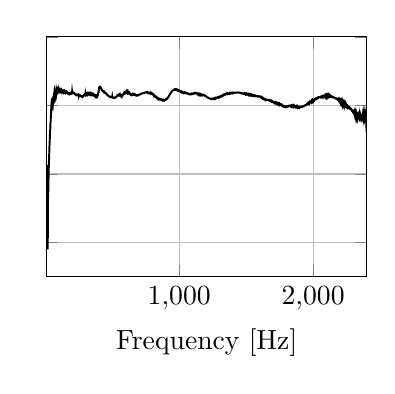
\begin{tikzpicture}

\begin{axis}[%
width=1.6in,
height=1.2in,
at={(1.011in,0.642in)},
scale only axis,
xmin=10,
xmax=2400,
xmajorgrids,
ymin=-30,
ymax=40,
ymajorgrids,
yticklabels={\empty},
xlabel={Frequency [Hz]},
axis background/.style={fill=white}
]
\addplot [color=black,line width=0.7pt,solid,forget plot]
  table[row sep=crcr]{%
0	-7.15873715654256\\
0.666675926054529	10.5087143459122\\
1.33335185210906	12.0967706112481\\
2.00002777816359	6.51246636920068\\
2.66670370421811	-0.175356461979414\\
3.33337963027264	-18.2069665387285\\
4.00005555632717	-15.6498849010992\\
4.6667314823817	-15.9720022096806\\
5.33340740843623	-12.3773277402846\\
6.00008333449076	-11.5127732534421\\
6.66675926054529	-13.124549272927\\
7.33343518659981	-16.8771871920024\\
8.00011111265434	-16.1609324436371\\
8.66678703870887	-16.3957874216142\\
9.3334629647634	-16.1414826002659\\
10.0001388908179	-9.11581854569876\\
10.6668148168725	2.63290680382195\\
11.333490742927	-1.30797727219537\\
12.0001666689815	-17.0636267744369\\
12.666842595036	-6.45026196358668\\
13.3335185210906	2.50663364486626\\
14.0001944471451	-1.70725075474316\\
14.6668703731996	-7.75658468652631\\
15.3335462992542	-9.3483774195719\\
16.0002222253087	-18.6218490262723\\
16.6668981513632	-9.45840899211946\\
17.3335740774177	-13.1140954030332\\
18.0002500034723	-21.9762082832002\\
18.6669259295268	-13.7328495691011\\
19.3336018555813	-11.8237285639594\\
20.0002777816359	-7.07261993440821\\
20.6669537076904	-6.4186096602619\\
21.3336296337449	-6.18112723880758\\
22.0003055597994	-3.42930466318585\\
22.666981485854	-5.04669005883661\\
23.3336574119085	-1.90200540857826\\
24.000333337963	-1.10164436043141\\
24.6670092640176	-0.272686762586023\\
25.3336851900721	1.2811352009495\\
26.0003611161266	2.57386832992159\\
26.6670370421811	2.79701323911136\\
27.3337129682357	3.92461706055076\\
28.0003888942902	4.5923075236652\\
28.6670648203447	5.33513322771373\\
29.3337407463993	6.22858231433341\\
30.0004166724538	6.93789285053402\\
30.6670925985083	7.88093877259057\\
31.3337685245628	8.5797174595324\\
32.0004444506174	9.13987555426015\\
32.6671203766719	9.69391198570301\\
33.3337963027264	10.471697172567\\
34.000472228781	11.2413498429474\\
34.6671481548355	11.9313674436524\\
35.33382408089	12.2206834471294\\
36.0005000069445	12.4355316665065\\
36.6671759329991	12.91188971702\\
37.3338518590536	13.6710847637875\\
38.0005277851081	14.5877480302561\\
38.6672037111627	15.0387885738662\\
39.3338796372172	15.0711002975034\\
40.0005555632717	15.2830740834027\\
40.6672314893262	16.2003603604853\\
41.3339074153808	16.9396542771061\\
42.0005833414353	17.2297836019304\\
42.6672592674898	17.5510274709084\\
43.3339351935444	18.3321890658326\\
44.0006111195989	19.0009998728534\\
44.6672870456534	19.3218972962387\\
45.3339629717079	19.7636726486508\\
46.0006388977625	20.5788804567535\\
46.667314823817	21.0659799329833\\
47.3339907498715	21.0706724489368\\
48.0006666759261	21.2954081888215\\
48.6673426019806	21.7504295307416\\
49.3340185280351	22.0226222784184\\
50.0006944540896	21.2851160722985\\
50.6673703801442	21.2051107463812\\
51.3340463061987	21.2927606988301\\
52.0007222322532	20.8577882479969\\
52.6673981583078	20.6711600742184\\
53.3340740843623	20.9203469279752\\
54.0007500104168	20.8221912113757\\
54.6674259364713	20.6991382976059\\
55.3341018625259	21.0407088483543\\
56.0007777885804	21.1298890830395\\
56.6674537146349	20.9530262480563\\
57.3341296406895	21.3766147555176\\
58.000805566744	21.5208537071508\\
58.6674814927985	21.2653058543976\\
59.334157418853	21.7307748662152\\
60.0008333449076	21.8951668040078\\
60.6675092709621	21.6512975974035\\
61.3341851970166	22.1294978753974\\
62.0008611230712	22.1845098242759\\
62.6675370491257	22.0945317033398\\
63.3342129751802	22.469571046389\\
64.0008889012347	22.4144126743392\\
64.6675648272893	22.4656633253754\\
65.3342407533438	22.7711307278621\\
66.0009166793983	22.595344049128\\
66.6675926054529	22.8211361901548\\
67.3342685315074	22.9714363429243\\
68.0009444575619	22.7483408524739\\
68.6676203836164	23.1900991734327\\
69.334296309671	23.0139565502041\\
70.0009722357255	23.0078941437368\\
70.66764816178	23.2640888008504\\
71.3343240878346	23.0521172453856\\
72.0010000138891	23.2968321488529\\
72.6676759399436	23.2063136781876\\
73.3343518659981	23.3339191542813\\
74.0010277920527	23.4201131005648\\
74.6677037181072	23.2737916065581\\
75.3343796441617	23.6255319273586\\
76.0010555702163	23.3345039510527\\
76.6677314962708	23.6224375724773\\
77.3344074223253	23.6114616424184\\
78.0010833483798	23.656576732508\\
78.6677592744344	23.7364151810855\\
79.3344352004889	23.7429745501262\\
80.0011111265434	23.8351365589793\\
80.667787052598	23.7447631942601\\
81.3344629786525	24.0074055842899\\
82.001138904707	23.8089022197667\\
82.6678148307615	24.0822291816178\\
83.3344907568161	23.9694717725242\\
84.0011666828706	24.1099258580291\\
84.6678426089251	24.0718306679598\\
85.3345185349797	24.2264814415983\\
86.0011944610342	24.1215006110483\\
86.6678703870887	24.2884169849204\\
87.3345463131432	24.2187384264903\\
88.0012222391978	24.3234554885306\\
88.6678981652523	24.3334222819882\\
89.3345740913068	24.3419120374625\\
90.0012500173614	24.3674475386358\\
90.6679259434159	24.4128618208234\\
91.3346018694704	24.3605904365201\\
92.0012777955249	24.490939092038\\
92.6679537215795	24.3883742537234\\
93.334629647634	24.5004186810227\\
94.0013055736885	24.4553094468998\\
94.667981499743	24.5035723715013\\
95.3346574257976	24.4446167778904\\
96.0013333518521	24.5316501403195\\
96.6680092779066	24.4406424070208\\
97.3346852039612	24.5138592854188\\
98.0013611300157	24.4334755790068\\
98.6680370560702	24.4430074171027\\
99.3347129821248	24.4448643874685\\
100.001388908179	24.5830026648291\\
100.668064834234	24.4380232462697\\
101.334740760288	24.367009642005\\
102.001416686343	24.4193073708642\\
102.668092612397	24.3062601108404\\
103.334768538452	24.3793294237293\\
104.001444464506	24.3564597657447\\
104.668120390561	24.3049224218097\\
105.334796316616	24.3674642786709\\
106.00147224267	24.2796963564791\\
106.668148168725	24.3472237616032\\
107.334824094779	24.3024466459277\\
108.001500020834	24.3293347604687\\
108.668175946888	24.3346573062107\\
109.334851872943	24.2937502414376\\
110.001527798997	24.3130074916196\\
110.668203725052	24.3272388220414\\
111.334879651106	24.3171147618053\\
112.001555577161	24.3363629515837\\
112.668231503215	24.3164517932769\\
113.33490742927	24.2788172766694\\
114.001583355324	24.353623658134\\
114.668259281379	24.2556978272775\\
115.334935207433	24.3056736662729\\
116.001611133488	24.2935033143821\\
116.668287059542	24.3115581567028\\
117.334962985597	24.2841837577282\\
118.001638911652	24.3345410688641\\
118.668314837706	24.2299614327879\\
119.334990763761	24.3242644212272\\
120.001666689815	24.2642435178612\\
120.66834261587	24.2865744746116\\
121.335018541924	24.2362265269981\\
122.001694467979	24.2878326149751\\
122.668370394033	24.199568432106\\
123.335046320088	24.2548448168798\\
124.001722246142	24.221737207819\\
124.668398172197	24.2279796362291\\
125.335074098251	24.1628143444844\\
126.001750024306	24.1726631684249\\
126.66842595036	24.1405365714659\\
127.335101876415	24.1014505663823\\
128.001777802469	24.1264812205878\\
128.668453728524	24.0820035236455\\
129.335129654579	24.0995864301708\\
130.001805580633	24.0159117359564\\
130.668481506688	24.0696150031467\\
131.335157432742	23.9974759426067\\
132.001833358797	24.0274658229844\\
132.668509284851	23.9846347041687\\
133.335185210906	24.0053856625507\\
134.00186113696	24.0257414417826\\
134.668537063015	23.9705604936007\\
135.335212989069	24.0116275950592\\
136.001888915124	23.9385430358016\\
136.668564841178	24.003448783508\\
137.335240767233	23.9357430250413\\
138.001916693287	23.9267099430717\\
138.668592619342	23.9397502148012\\
139.335268545396	23.9019035587597\\
140.001944471451	23.9667578531696\\
140.668620397506	23.9002705054755\\
141.33529632356	23.9301926792168\\
142.001972249615	23.9274379783929\\
142.668648175669	23.9107077654991\\
143.335324101724	23.9708240066973\\
144.002000027778	23.8976416979434\\
144.668675953833	23.9280605624893\\
145.335351879887	23.9395178290452\\
146.002027805942	23.9104477198023\\
146.668703731996	24.0042861899005\\
147.335379658051	23.9593716743793\\
148.002055584105	23.9548869966147\\
148.66873151016	23.9741124268126\\
149.335407436214	23.9137084328685\\
150.002083362269	24.0358334053608\\
150.668759288323	24.0129356581571\\
151.335435214378	23.9783044375457\\
152.002111140433	24.0135243729903\\
152.668787066487	23.9570176164768\\
153.335462992542	23.9373671861388\\
154.002138918596	24.0099718833998\\
154.668814844651	23.992175802195\\
155.335490770705	23.9905852435095\\
156.00216669676	24.0154380181123\\
156.668842622814	23.9448424581498\\
157.335518548869	23.9282342359544\\
158.002194474923	23.9412155054648\\
158.668870400978	23.8551568215683\\
159.335546327032	23.8452894749057\\
160.002222253087	23.881183650396\\
160.668898179141	23.8200251691604\\
161.335574105196	23.7885210433908\\
162.00225003125	23.8000977308225\\
162.668925957305	23.7368248711784\\
163.335601883359	23.6809154091656\\
164.002277809414	23.6665957710001\\
164.668953735469	23.6251820323242\\
165.335629661523	23.5786949380226\\
166.002305587578	23.5889468796819\\
166.668981513632	23.5848149862382\\
167.335657439687	23.5652098311667\\
168.002333365741	23.5511967971205\\
168.669009291796	23.5733584242023\\
169.33568521785	23.5538389244039\\
170.002361143905	23.5127478614158\\
170.669037069959	23.5456375024997\\
171.335712996014	23.537627613085\\
172.002388922068	23.4590023938168\\
172.669064848123	23.4686637651834\\
173.335740774177	23.4939816310679\\
174.002416700232	23.4211397740851\\
174.669092626286	23.3974198931325\\
175.335768552341	23.4132330294167\\
176.002444478396	23.4159270564024\\
176.66912040445	23.3919798536214\\
177.335796330505	23.3549185868886\\
178.002472256559	23.409420195141\\
178.669148182614	23.4296019615359\\
179.335824108668	23.3943393217074\\
180.002500034723	23.4064345494135\\
180.669175960777	23.4276710326754\\
181.335851886832	23.4763933629542\\
182.002527812886	23.4551022379621\\
182.669203738941	23.4466717248939\\
183.335879664995	23.4944683083156\\
184.00255559105	23.5051198154288\\
184.669231517104	23.521638340073\\
185.335907443159	23.4895152375784\\
186.002583369213	23.5116009885307\\
186.669259295268	23.5245887945761\\
187.335935221323	23.5634160727353\\
188.002611147377	23.5180171818616\\
188.669287073432	23.5007882491574\\
189.335962999486	23.4703268300687\\
190.002638925541	23.5218474907648\\
190.669314851595	23.5117957925876\\
191.33599077765	23.5073489030819\\
192.002666703704	23.4748867900627\\
192.669342629759	23.5238532127275\\
193.336018555813	23.5443500501714\\
194.002694481868	23.6052564056829\\
194.669370407922	23.6032195687775\\
195.336046333977	23.6067703614072\\
196.002722260031	23.6081462118097\\
196.669398186086	23.6284913263107\\
197.33607411214	23.6683757100492\\
198.002750038195	23.6500605877708\\
198.66942596425	23.6602688200448\\
199.336101890304	23.6430623940489\\
200.002777816359	23.9325844631997\\
200.669453742413	23.7295267431329\\
201.336129668468	23.7453272006813\\
202.002805594522	23.7956790146267\\
202.669481520577	23.7648214347693\\
203.336157446631	23.7392293326182\\
204.002833372686	23.732937791739\\
204.66950929874	23.7163043256602\\
205.336185224795	23.7762496457566\\
206.002861150849	23.8173995548699\\
206.669537076904	23.819690576325\\
207.336213002958	23.8133007788291\\
208.002888929013	23.7553494306647\\
208.669564855067	23.7263702197232\\
209.336240781122	23.7427961208167\\
210.002916707176	23.7457006858622\\
210.669592633231	23.7430014060931\\
211.336268559286	23.7336216256452\\
212.00294448534	23.690354867883\\
212.669620411395	23.664049586363\\
213.336296337449	23.6740149563915\\
214.002972263504	23.6470281106283\\
214.669648189558	23.5774503862567\\
215.336324115613	23.5200440720789\\
216.003000041667	23.501268482812\\
216.669675967722	23.4929198584724\\
217.336351893776	23.484777667757\\
218.003027819831	23.4627902735257\\
218.669703745885	23.4236067287961\\
219.33637967194	23.3896423123424\\
220.003055597994	23.3880062098513\\
220.669731524049	23.360435599666\\
221.336407450103	23.295373972138\\
222.003083376158	23.2435794936051\\
222.669759302213	23.2154136066346\\
223.336435228267	23.1782769365077\\
224.003111154322	23.1475453537114\\
224.669787080376	23.1410471008364\\
225.336463006431	23.1401937937074\\
226.003138932485	23.112688490254\\
226.66981485854	23.0846909271996\\
227.336490784594	23.1030816728332\\
228.003166710649	23.1383110228286\\
228.669842636703	23.0984731681706\\
229.336518562758	23.0754664321036\\
230.003194488812	23.1070024213092\\
230.669870414867	23.1393155792247\\
231.336546340921	23.1138425882487\\
232.003222266976	23.1025528200807\\
232.66989819303	23.0919111899043\\
233.336574119085	23.0269870112512\\
234.00325004514	22.9891308460617\\
234.669925971194	22.9989878077763\\
235.336601897249	23.0044408853645\\
236.003277823303	23.0079139293434\\
236.669953749358	23.053827118727\\
237.336629675412	23.0753116048292\\
238.003305601467	23.0506572130619\\
238.669981527521	23.0938313946732\\
239.336657453576	23.0801118803019\\
240.00333337963	23.0578906249399\\
240.670009305685	23.0979644782169\\
241.336685231739	23.0812668912868\\
242.003361157794	23.0627709669134\\
242.670037083848	23.098894118898\\
243.336713009903	23.0788132473687\\
244.003388935957	23.0869290004178\\
244.670064862012	23.1165807061338\\
245.336740788066	23.0898887826167\\
246.003416714121	23.1126726466507\\
246.670092640176	23.1194517032361\\
247.33676856623	23.0749178994239\\
248.003444492285	23.1072615007923\\
248.670120418339	23.0712759311162\\
249.336796344394	23.0631772802676\\
250.003472270448	22.8922414185675\\
250.670148196503	23.0048298809381\\
251.336824122557	23.0190106554729\\
252.003500048612	22.9874843352767\\
252.670175974666	22.9728118289677\\
253.336851900721	22.982477272407\\
254.003527826775	22.9583179686267\\
254.67020375283	22.9952054740954\\
255.336879678884	22.971121774093\\
256.003555604939	22.9865498886205\\
256.670231530993	22.9807406944549\\
257.336907457048	22.9681666605489\\
258.003583383103	22.9768272202065\\
258.670259309157	22.9192668609388\\
259.336935235212	22.9353555559673\\
260.003611161266	22.8702712699718\\
260.670287087321	22.8697452401716\\
261.336963013375	22.8121830398662\\
262.00363893943	22.81443725079\\
262.670314865484	22.7909267714697\\
263.336990791539	22.7905444968254\\
264.003666717593	22.7798958806609\\
264.670342643648	22.7740146447856\\
265.337018569702	22.7604926592849\\
266.003694495757	22.716614209319\\
266.670370421811	22.7021420662505\\
267.337046347866	22.6644170005054\\
268.00372227392	22.675102369387\\
268.670398199975	22.6585656693192\\
269.33707412603	22.6845816113223\\
270.003750052084	22.6737527254366\\
270.670425978139	22.6463608482636\\
271.337101904193	22.5953795718538\\
272.003777830248	22.5635895606184\\
272.670453756302	22.5674031766485\\
273.337129682357	22.5964060389313\\
274.003805608411	22.6309677360793\\
274.670481534466	22.6240231221093\\
275.33715746052	22.6236841124181\\
276.003833386575	22.5823719455308\\
276.670509312629	22.6111455283201\\
277.337185238684	22.5836961851879\\
278.003861164738	22.6328828994838\\
278.670537090793	22.6388029436635\\
279.337213016847	22.6636737409649\\
280.003888942902	22.6136392098819\\
280.670564868956	22.5802448996619\\
281.337240795011	22.6276271133216\\
282.003916721066	22.6693610695881\\
282.67059264712	22.7209756588301\\
283.337268573175	22.6859101869821\\
284.003944499229	22.7008570077434\\
284.670620425284	22.7234674390024\\
285.337296351338	22.7574004388151\\
286.003972277393	22.8445229709759\\
286.670648203447	22.8422932014905\\
287.337324129502	22.8336215459351\\
288.004000055556	22.8534736044996\\
288.670675981611	22.913823952474\\
289.337351907665	22.9758039708997\\
290.00402783372	22.9447318473799\\
290.670703759774	22.9535210499885\\
291.337379685829	22.9705623129775\\
292.004055611883	23.0256758850494\\
292.670731537938	23.0820633636433\\
293.337407463993	23.0286917736661\\
294.004083390047	23.027952961887\\
294.670759316102	23.1006304178873\\
295.337435242156	23.1056682211187\\
296.004111168211	23.1028400500452\\
296.670787094265	23.081667088508\\
297.33746302032	23.1088261705323\\
298.004138946374	23.1642148879404\\
298.670814872429	23.1531093623504\\
299.337490798483	23.1166864464385\\
300.004166724538	23.3665418070538\\
300.670842650592	23.2281860870225\\
301.337518576647	23.1662682127715\\
302.004194502701	23.1544402143831\\
302.670870428756	23.2342783454354\\
303.33754635481	23.2397236487141\\
304.004222280865	23.2038218162903\\
304.67089820692	23.207616142466\\
305.337574132974	23.2821001817681\\
306.004250059029	23.2330287871902\\
306.670925985083	23.2131033861347\\
307.337601911138	23.2352914154204\\
308.004277837192	23.2795248232929\\
308.670953763247	23.2099013595069\\
309.337629689301	23.2388779697744\\
310.004305615356	23.2800594659038\\
310.67098154141	23.2569280486767\\
311.337657467465	23.2114638342554\\
312.004333393519	23.299609424179\\
312.671009319574	23.2954833083898\\
313.337685245628	23.2558224068988\\
314.004361171683	23.2986141599806\\
314.671037097737	23.3661936285544\\
315.337713023792	23.312169742643\\
316.004388949847	23.3170811893786\\
316.671064875901	23.381741441126\\
317.337740801956	23.3355333422287\\
318.00441672801	23.3836132273774\\
318.671092654065	23.4126914826485\\
319.337768580119	23.3752190931115\\
320.004444506174	23.3986670195967\\
320.671120432228	23.4516374896275\\
321.337796358283	23.4144777344401\\
322.004472284337	23.3988945127971\\
322.671148210392	23.4423603982258\\
323.337824136446	23.4031282824876\\
324.004500062501	23.4396809699807\\
324.671175988555	23.4541101356225\\
325.33785191461	23.3771322764977\\
326.004527840664	23.4192964497452\\
326.671203766719	23.4264931341787\\
327.337879692774	23.3914217573799\\
328.004555618828	23.4557960765174\\
328.671231544883	23.4043099290427\\
329.337907470937	23.3937384344687\\
330.004583396992	23.4275941623696\\
330.671259323046	23.388045098902\\
331.337935249101	23.4432486139232\\
332.004611175155	23.4052667657364\\
332.67128710121	23.400573463867\\
333.337963027264	23.4401434219522\\
334.004638953319	23.357845359059\\
334.671314879373	23.4112267792951\\
335.337990805428	23.4006761429916\\
336.004666731482	23.3773302892184\\
336.671342657537	23.4304678684814\\
337.338018583591	23.3759822922548\\
338.004694509646	23.4198373123268\\
338.671370435701	23.3524395927385\\
339.338046361755	23.3533348287594\\
340.00472228781	23.3711708407037\\
340.671398213864	23.3132864465162\\
341.338074139919	23.3642997499883\\
342.004750065973	23.2957960291322\\
342.671425992028	23.3514068730671\\
343.338101918082	23.3257420257991\\
344.004777844137	23.3174921853021\\
344.671453770191	23.3031464955361\\
345.338129696246	23.263620991949\\
346.0048056223	23.3083246315707\\
346.671481548355	23.2417673165442\\
347.338157474409	23.2851718739417\\
348.004833400464	23.204452393028\\
348.671509326518	23.2326993738068\\
349.338185252573	23.1862953150634\\
350.004861178627	23.2024954774285\\
350.671537104682	23.2016188891564\\
351.338213030737	23.1974198598719\\
352.004888956791	23.1970438821182\\
352.671564882846	23.1711529885069\\
353.3382408089	23.2037763664283\\
354.004916734955	23.1677641995215\\
354.671592661009	23.2069921649515\\
355.338268587064	23.1650070213611\\
356.004944513118	23.1992209603012\\
356.671620439173	23.1409738539685\\
357.338296365227	23.1788912067377\\
358.004972291282	23.1027019847916\\
358.671648217336	23.1476111249839\\
359.338324143391	23.0786920764213\\
360.005000069445	23.1226919519339\\
360.6716759955	23.0611148901713\\
361.338351921554	23.092286326067\\
362.005027847609	23.0470916754452\\
362.671703773664	23.0664222074796\\
363.338379699718	23.0238804328784\\
364.005055625773	23.035169672148\\
364.671731551827	23.0093452500552\\
365.338407477882	22.9938314216959\\
366.005083403936	22.9830093396502\\
366.671759329991	22.950682957497\\
367.338435256045	22.9652681177984\\
368.0051111821	22.9115777998351\\
368.671787108154	22.9378777062769\\
369.338463034209	22.8725537469231\\
370.005138960263	22.9078087983924\\
370.671814886318	22.8444563514053\\
371.338490812372	22.8702265014038\\
372.005166738427	22.823562456798\\
372.671842664481	22.8208599571976\\
373.338518590536	22.8111223570435\\
374.005194516591	22.7522474525364\\
374.671870442645	22.7817476427405\\
375.3385463687	22.6941969850737\\
376.005222294754	22.7383231711478\\
376.671898220809	22.6754846835769\\
377.338574146863	22.6877581861511\\
378.005250072918	22.6906717089616\\
378.671925998972	22.658351924489\\
379.338601925027	22.705607335846\\
380.005277851081	22.6429832893611\\
380.671953777136	22.6691583584912\\
381.33862970319	22.6194392027024\\
382.005305629245	22.5757695192077\\
382.671981555299	22.5905242397834\\
383.338657481354	22.5197369972299\\
384.005333407408	22.5456802402232\\
384.672009333463	22.5340064505076\\
385.338685259517	22.5096147354606\\
386.005361185572	22.5682871856995\\
386.672037111627	22.5213255359728\\
387.338713037681	22.5711912354341\\
388.005388963736	22.625259679459\\
388.67206488979	22.6288198538351\\
389.338740815845	22.7603325712579\\
390.005416741899	22.8129192557627\\
390.672092667954	22.8784920405188\\
391.338768594008	23.0206437879727\\
392.005444520063	23.0769470015594\\
392.672120446117	23.2209934474768\\
393.338796372172	23.3752791549899\\
394.005472298226	23.4317600457901\\
394.672148224281	23.5820447454569\\
395.338824150335	23.7302811865809\\
396.00550007639	23.8240416597948\\
396.672176002444	24.0128021996323\\
397.338851928499	24.1482868134601\\
398.005527854554	24.2360199546688\\
398.672203780608	24.4474335771642\\
399.338879706663	24.6038826762412\\
400.005555632717	24.5605666726398\\
400.672231558772	24.8100488703285\\
401.338907484826	24.9634337837249\\
402.005583410881	25.0224017171142\\
402.672259336935	25.1189085776965\\
403.33893526299	25.235563413276\\
404.005611189044	25.2717036553352\\
404.672287115099	25.3314128075437\\
405.338963041153	25.3991343019002\\
406.005638967208	25.3935888823572\\
406.672314893262	25.3965680663757\\
407.338990819317	25.4356907615614\\
408.005666745371	25.4272133150631\\
408.672342671426	25.366634698988\\
409.339018597481	25.3729685396194\\
410.005694523535	25.3840453400317\\
410.67237044959	25.2965949046627\\
411.339046375644	25.2510525177916\\
412.005722301699	25.2758580500552\\
412.672398227753	25.2077616573045\\
413.339074153808	25.1164201027822\\
414.005750079862	25.1016445456299\\
414.672426005917	25.058259510491\\
415.339101931971	24.9882349890131\\
416.005777858026	24.9181123919607\\
416.67245378408	24.8757656863904\\
417.339129710135	24.8858751028074\\
418.005805636189	24.8112830993537\\
418.672481562244	24.7362554872007\\
419.339157488298	24.7263307536006\\
420.005833414353	24.7389744979165\\
420.672509340407	24.6800214622345\\
421.339185266462	24.5843610206647\\
422.005861192517	24.6022249994799\\
422.672537118571	24.5761496535907\\
423.339213044626	24.5646465042338\\
424.00588897068	24.4752897618484\\
424.672564896735	24.4285861432201\\
425.339240822789	24.4314731468244\\
426.005916748844	24.3979437025808\\
426.672592674898	24.3015094891424\\
427.339268600953	24.2545541748938\\
428.005944527007	24.2328455773834\\
428.672620453062	24.2737375769304\\
429.339296379116	24.2632491902619\\
430.005972305171	24.2057651955647\\
430.672648231225	24.1714503299811\\
431.33932415728	24.1623235443258\\
432.006000083334	24.1842873641646\\
432.672676009389	24.1828452161925\\
433.339351935444	24.1055814305408\\
434.006027861498	24.09285264821\\
434.672703787553	24.047628526424\\
435.339379713607	24.0911791492153\\
436.006055639662	24.0617381755948\\
436.672731565716	24.0487885524772\\
437.339407491771	23.9880694116177\\
438.006083417825	23.9276842342827\\
438.67275934388	23.9472251782106\\
439.339435269934	23.9199627050903\\
440.006111195989	23.9538873760375\\
440.672787122043	23.892317954538\\
441.339463048098	23.8535029673726\\
442.006138974152	23.813718178514\\
442.672814900207	23.7912046507748\\
443.339490826261	23.8011827237526\\
444.006166752316	23.8067842569663\\
444.672842678371	23.7821685741767\\
445.339518604425	23.7650070458023\\
446.00619453048	23.7125347109658\\
446.672870456534	23.6612109064161\\
447.339546382589	23.6582383057953\\
448.006222308643	23.6397043370453\\
448.672898234698	23.6398786909826\\
449.339574160752	23.6475041293184\\
450.006250086807	23.6220633837197\\
450.672926012861	23.5705148100686\\
451.339601938916	23.5441797931312\\
452.00627786497	23.4955456219766\\
452.672953791025	23.4503897931678\\
453.339629717079	23.4563352286849\\
454.006305643134	23.4331579273573\\
454.672981569188	23.425576157168\\
455.339657495243	23.4023542595\\
456.006333421298	23.4164633563494\\
456.673009347352	23.3596926012022\\
457.339685273407	23.329539130947\\
458.006361199461	23.282100168342\\
458.673037125516	23.2645172262514\\
459.33971305157	23.211896289963\\
460.006388977625	23.1642517273922\\
460.673064903679	23.1451054452469\\
461.339740829734	23.1215301660216\\
462.006416755788	23.1271164476067\\
462.673092681843	23.0785693515525\\
463.339768607897	23.0677163935001\\
464.006444533952	23.0535931639354\\
464.673120460006	23.0373979010306\\
465.339796386061	23.0214724946777\\
466.006472312115	22.9684360172689\\
466.67314823817	22.9492822646665\\
467.339824164225	22.9205703994463\\
468.006500090279	22.8892631135468\\
468.673176016334	22.8842417485463\\
469.339851942388	22.8362122012308\\
470.006527868443	22.8121458874946\\
470.673203794497	22.7881002412262\\
471.339879720552	22.7517999758853\\
472.006555646606	22.7575020839074\\
472.673231572661	22.7344592916752\\
473.339907498715	22.7201364600742\\
474.00658342477	22.7110151487217\\
474.673259350824	22.6790260133921\\
475.339935276879	22.6566296224347\\
476.006611202933	22.6398455086865\\
476.673287128988	22.6107385911572\\
477.339963055042	22.5921911313787\\
478.006638981097	22.5889108793928\\
478.673314907152	22.5665846391812\\
479.339990833206	22.5654983876713\\
480.006666759261	22.5764465071147\\
480.673342685315	22.5512033056028\\
481.34001861137	22.5359062912685\\
482.006694537424	22.5332557232302\\
482.673370463479	22.5096901998091\\
483.340046389533	22.4847600438032\\
484.006722315588	22.4827123785872\\
484.673398241642	22.4748141311656\\
485.340074167697	22.4535139679094\\
486.006750093751	22.4558405256336\\
486.673426019806	22.4576923512691\\
487.34010194586	22.4480277084016\\
488.006777871915	22.452118245327\\
488.673453797969	22.4723476677798\\
489.340129724024	22.4790314240742\\
490.006805650078	22.4701324928377\\
490.673481576133	22.4710256311865\\
491.340157502188	22.4746986008659\\
492.006833428242	22.458796802072\\
492.673509354297	22.436710203806\\
493.340185280351	22.4285228065914\\
494.006861206406	22.42974129422\\
494.67353713246	22.4146014883439\\
495.340213058515	22.3918596302885\\
496.006888984569	22.3873433462568\\
496.673564910624	22.4011294188386\\
497.340240836678	22.3993600031334\\
498.006916762733	22.3934189857785\\
498.673592688787	22.3959247581123\\
499.340268614842	22.3980804467826\\
500.006944540896	22.5556762884854\\
500.673620466951	22.3974492753894\\
501.340296393005	22.368857290977\\
502.00697231906	22.3462530764068\\
502.673648245115	22.3367616084347\\
503.340324171169	22.3236330454825\\
504.007000097224	22.3130497843336\\
504.673676023278	22.3087159923272\\
505.340351949333	22.3151007138196\\
506.007027875387	22.3309347341289\\
506.673703801442	22.3260035011254\\
507.340379727496	22.3026852159121\\
508.007055653551	22.2700563983849\\
508.673731579605	22.2289702448306\\
509.34040750566	22.227819946724\\
510.007083431714	22.2524631932524\\
510.673759357769	22.2852562256613\\
511.340435283823	22.2885169498584\\
512.007111209878	22.2530696843343\\
512.673787135932	22.2161262023443\\
513.340463061987	22.1976125470916\\
514.007138988041	22.222057758885\\
514.673814914096	22.2408173670611\\
515.340490840151	22.2532140444528\\
516.007166766205	22.255704132218\\
516.67384269226	22.2528469180602\\
517.340518618314	22.2412670775663\\
518.007194544369	22.2302604231504\\
518.673870470423	22.2580699907529\\
519.340546396478	22.2960580258133\\
520.007222322532	22.3215956694387\\
520.673898248587	22.292711184102\\
521.340574174641	22.2921542442947\\
522.007250100696	22.3191795064228\\
522.67392602675	22.3555140919138\\
523.340601952805	22.364265945962\\
524.007277878859	22.3797601749284\\
524.673953804914	22.3714415496905\\
525.340629730968	22.3680027167281\\
526.007305657023	22.4088621026103\\
526.673981583078	22.4640973821973\\
527.340657509132	22.4601723889253\\
528.007333435187	22.4487260807839\\
528.674009361241	22.4783243839663\\
529.340685287296	22.5159768553421\\
530.00736121335	22.5684477666636\\
530.674037139405	22.578746650228\\
531.340713065459	22.5672010872706\\
532.007388991514	22.613410184191\\
532.674064917568	22.6720092349587\\
533.340740843623	22.6848708485002\\
534.007416769677	22.7004009522696\\
534.674092695732	22.7033647144998\\
535.340768621786	22.7570213247332\\
536.007444547841	22.8066157979055\\
536.674120473896	22.7771235107182\\
537.34079639995	22.8103882371864\\
538.007472326005	22.8508287683496\\
538.674148252059	22.8809487827767\\
539.340824178114	22.8822835892378\\
540.007500104168	22.872836926273\\
540.674176030223	22.9409284225212\\
541.340851956277	22.9486301332984\\
542.007527882332	22.9503051462533\\
542.674203808386	22.9440067977203\\
543.340879734441	23.0121243840464\\
544.007555660495	23.0034512520761\\
544.67423158655	22.9891208696874\\
545.340907512604	23.010790639817\\
546.007583438659	23.0600250441806\\
546.674259364713	23.0299195345168\\
547.340935290768	23.0281484988089\\
548.007611216823	23.0740637133528\\
548.674287142877	23.076494011509\\
549.340963068932	23.0433162692488\\
550.007638994986	23.0889741013555\\
550.674314921041	23.1153192163153\\
551.340990847095	23.0904431790381\\
552.00766677315	23.0948912368854\\
552.674342699204	23.1411827306395\\
553.341018625259	23.0798824324349\\
554.007694551313	23.0976578046195\\
554.674370477368	23.1022173080237\\
555.341046403422	23.0775136151027\\
556.007722329477	23.0423404850017\\
556.674398255531	23.0845663505847\\
557.341074181586	23.0514846409615\\
558.00775010764	23.0222442900952\\
558.674426033695	23.0781988252938\\
559.341101959749	23.0016519343541\\
560.007777885804	22.9867363234617\\
560.674453811858	22.9995238939942\\
561.341129737913	22.9182260060531\\
562.007805663968	22.9071470208661\\
562.674481590022	22.8978954225745\\
563.341157516077	22.8276167423139\\
564.007833442131	22.8319379404363\\
564.674509368186	22.7980293203263\\
565.34118529424	22.7236366916712\\
566.007861220295	22.7328069820359\\
566.674537146349	22.6729735942675\\
567.341213072404	22.6476000823122\\
568.007888998458	22.6909341331093\\
568.674564924513	22.6183503679082\\
569.341240850567	22.6432736310698\\
570.007916776622	22.6595463287102\\
570.674592702676	22.6097747623807\\
571.341268628731	22.6929377403755\\
572.007944554785	22.7009934548951\\
572.67462048084	22.7021026774696\\
573.341296406895	22.7551728416182\\
574.007972332949	22.7505180240948\\
574.674648259004	22.8222548355523\\
575.341324185058	22.8412596694343\\
576.008000111113	22.8731501858362\\
576.674676037167	22.9496451050659\\
577.341351963222	22.9433182519649\\
578.008027889276	23.0342522269302\\
578.674703815331	23.0519341435632\\
579.341379741385	23.1121322335299\\
580.00805566744	23.1400469619068\\
580.674731593494	23.1552000982357\\
581.341407519549	23.2507566754524\\
582.008083445603	23.2489658838062\\
582.674759371658	23.3347560867854\\
583.341435297712	23.3344325894672\\
584.008111223767	23.4044509373415\\
584.674787149822	23.4331699427611\\
585.341463075876	23.4618953372666\\
586.008139001931	23.5328919450315\\
586.674814927985	23.5284988425091\\
587.34149085404	23.5757448014353\\
588.008166780094	23.5550104373674\\
588.674842706149	23.6571778406404\\
589.341518632203	23.6381512968117\\
590.008194558258	23.6965635088613\\
590.674870484312	23.6916376623203\\
591.341546410367	23.7451371180211\\
592.008222336421	23.7191740388327\\
592.674898262476	23.7718895764984\\
593.34157418853	23.8017976003933\\
594.008250114585	23.8229117895531\\
594.674926040639	23.8386868529616\\
595.341601966694	23.8782268859547\\
596.008277892749	23.8810183635803\\
596.674953818803	23.8756709635537\\
597.341629744858	23.9056998399092\\
598.008305670912	23.9031421113195\\
598.674981596967	23.9181515628447\\
599.341657523021	23.9508634240059\\
600.008333449076	23.8805873602388\\
600.67500937513	23.9622586843332\\
601.341685301185	23.9889985800693\\
602.008361227239	24.0026376782776\\
602.675037153294	23.9904799879627\\
603.341713079348	24.0386198925986\\
604.008389005403	23.9880625043385\\
604.675064931457	24.0611437363596\\
605.341740857512	24.0076429547272\\
606.008416783566	24.0519202565057\\
606.675092709621	24.0169048599477\\
607.341768635676	24.0588644656048\\
608.00844456173	24.0125309286435\\
608.675120487785	24.066765564531\\
609.341796413839	24.0119546403279\\
610.008472339894	24.0349107153302\\
610.675148265948	24.0239681379336\\
611.341824192003	23.9930567324848\\
612.008500118057	24.0367278043696\\
612.675176044112	23.9427825836015\\
613.341851970166	24.0136383106808\\
614.008527896221	23.9260728870395\\
614.675203822275	23.967874560845\\
615.34187974833	23.9386309128271\\
616.008555674384	23.9121841921643\\
616.675231600439	23.9527786815655\\
617.341907526493	23.8708946197959\\
618.008583452548	23.9409060531761\\
618.675259378603	23.869758995315\\
619.341935304657	23.8912419070363\\
620.008611230711	23.8831161386137\\
620.675287156766	23.8208071598346\\
621.341963082821	23.8456012404703\\
622.008639008875	23.7799195903703\\
622.67531493493	23.7539739552072\\
623.341990860984	23.7712922896337\\
624.008666787039	23.7059846392007\\
624.675342713093	23.736307461616\\
625.342018639148	23.7057318597623\\
626.008694565202	23.6457567355793\\
626.675370491257	23.6704860752896\\
627.342046417311	23.5846152449446\\
628.008722343366	23.5929820263484\\
628.67539826942	23.5927149191422\\
629.342074195475	23.534178373717\\
630.008750121529	23.5378234635832\\
630.675426047584	23.4899142794554\\
631.342101973638	23.4418013879416\\
632.008777899693	23.4648643283008\\
632.675453825748	23.4200253179656\\
633.342129751802	23.3738336644112\\
634.008805677857	23.3746893631768\\
634.675481603911	23.3017077656367\\
635.342157529966	23.3145078132275\\
636.00883345602	23.2782471960621\\
636.675509382075	23.2271912459278\\
637.342185308129	23.1865933222311\\
638.008861234184	23.2035485789039\\
638.675537160238	23.1457123345192\\
639.342213086293	23.1202529941746\\
640.008889012347	23.1266392408424\\
640.675564938402	23.0712377604073\\
641.342240864456	23.0985516195479\\
642.008916790511	23.0707215012686\\
642.675592716565	23.0583808867183\\
643.34226864262	23.0722746298861\\
644.008944568675	23.0757854678728\\
644.675620494729	23.0775737190015\\
645.342296420784	23.0655170251614\\
646.008972346838	23.1075933430503\\
646.675648272893	23.1032873247139\\
647.342324198947	23.0881326919386\\
648.009000125002	23.1283171868152\\
648.675676051056	23.1461635053042\\
649.342351977111	23.1451561411158\\
650.009027903165	23.1274044321186\\
650.67570382922	23.174074062497\\
651.342379755274	23.2165995015894\\
652.009055681329	23.1523605789994\\
652.675731607383	23.1796478983035\\
653.342407533438	23.2426741944987\\
654.009083459492	23.1942652917014\\
654.675759385547	23.1872648005046\\
655.342435311602	23.2039010623998\\
656.009111237656	23.2250070747326\\
656.675787163711	23.2131701195773\\
657.342463089765	23.1764770776587\\
658.00913901582	23.2067951136444\\
658.675814941874	23.2103111549554\\
659.342490867929	23.2263659548199\\
660.009166793983	23.1517168329694\\
660.675842720038	23.1637425728063\\
661.342518646092	23.2204451817756\\
662.009194572147	23.1850833790367\\
662.675870498201	23.1417722565883\\
663.342546424256	23.1340666490165\\
664.00922235031	23.1814717589597\\
664.675898276365	23.1479593637174\\
665.342574202419	23.1414817988859\\
666.009250128474	23.1011237830234\\
666.675926054529	23.1083220487726\\
667.342601980583	23.1116942065265\\
668.009277906638	23.1384149423654\\
668.675953832692	23.0763671735842\\
669.342629758747	23.0473479102096\\
670.009305684801	23.0466727826005\\
670.675981610856	23.1066009084499\\
671.34265753691	23.0605356569891\\
672.009333462965	23.0274246531842\\
672.676009389019	22.9986773913877\\
673.342685315074	23.0164546496092\\
674.009361241128	23.0306657792978\\
674.676037167183	23.015501261291\\
675.342713093237	23.0101616378404\\
676.009389019292	22.9644256087\\
676.676064945346	22.9727508843167\\
677.342740871401	22.9493790455104\\
678.009416797456	22.9720288308553\\
678.67609272351	22.9863316519141\\
679.342768649565	22.9663997270916\\
680.009444575619	22.9487900422614\\
680.676120501674	22.9024513546758\\
681.342796427728	22.9107880874405\\
682.009472353783	22.9512499995849\\
682.676148279837	22.9612981646361\\
683.342824205892	22.9696963441367\\
684.009500131946	22.9278079765716\\
684.676176058001	22.8881528900286\\
685.342851984055	22.9077360090166\\
686.00952791011	22.9132862841628\\
686.676203836164	22.9225816221733\\
687.342879762219	22.9567514469161\\
688.009555688273	22.939182938288\\
688.676231614328	22.9343930613014\\
689.342907540382	22.9485481762084\\
690.009583466437	22.9323852669615\\
690.676259392492	22.9236160133126\\
691.342935318546	22.9385515667977\\
692.009611244601	22.9460275375806\\
692.676287170655	22.9449960614785\\
693.34296309671	22.9775047277762\\
694.009639022764	23.0168108491432\\
694.676314948819	23.0147278233748\\
695.342990874873	23.0151084387104\\
696.009666800928	23.0314915693083\\
696.676342726982	23.0319153938354\\
697.343018653037	23.0092193284002\\
698.009694579091	23.0079175857448\\
698.676370505146	23.0389134326495\\
699.3430464312	23.0635381375235\\
700.009722357255	23.0806113725207\\
700.676398283309	23.1070747387522\\
701.343074209364	23.1429198483529\\
702.009750135419	23.1821318274822\\
702.676426061473	23.2034371400095\\
703.343101987528	23.1972361966381\\
704.009777913582	23.2023769448256\\
704.676453839637	23.2129795901655\\
705.343129765691	23.2377456291667\\
706.009805691746	23.2388210269578\\
706.6764816178	23.2402446979098\\
707.343157543855	23.2436202256167\\
708.009833469909	23.2531139776697\\
708.676509395964	23.2677796546635\\
709.343185322018	23.2950853772041\\
710.009861248073	23.3161448556964\\
710.676537174127	23.3230767972559\\
711.343213100182	23.3224069034599\\
712.009889026236	23.3363894122506\\
712.676564952291	23.352376178701\\
713.343240878346	23.3746584756115\\
714.0099168044	23.3897376175182\\
714.676592730455	23.4187604304551\\
715.343268656509	23.4314457069027\\
716.009944582564	23.4470768869404\\
716.676620508618	23.4473138841561\\
717.343296434673	23.4513154347126\\
718.009972360727	23.4618164961054\\
718.676648286782	23.4664520548425\\
719.343324212836	23.48092191548\\
720.010000138891	23.4868694976053\\
720.676676064945	23.4959092099804\\
721.343351991	23.5049851450233\\
722.010027917054	23.5152913741979\\
722.676703843109	23.5305386459897\\
723.343379769163	23.5348326469472\\
724.010055695218	23.5445654417811\\
724.676731621273	23.5504991007689\\
725.343407547327	23.5531631573508\\
726.010083473382	23.5690583822292\\
726.676759399436	23.5758723707306\\
727.343435325491	23.5926090661921\\
728.010111251545	23.6072628360651\\
728.6767871776	23.623601748347\\
729.343463103654	23.6329335257597\\
730.010139029709	23.6459222342708\\
730.676814955763	23.6525980284254\\
731.343490881818	23.6563295422292\\
732.010166807872	23.6524490742021\\
732.676842733927	23.647184839444\\
733.343518659981	23.633493465175\\
734.010194586036	23.622250891434\\
734.67687051209	23.6159784217895\\
735.343546438145	23.6190783694874\\
736.0102223642	23.6297958549446\\
736.676898290254	23.6526501551071\\
737.343574216309	23.6853001046733\\
738.010250142363	23.701724678475\\
738.676926068418	23.7203608777794\\
739.343601994472	23.7284602507321\\
740.010277920527	23.7187965816374\\
740.676953846581	23.7005295945607\\
741.343629772636	23.6926600441393\\
742.01030569869	23.6987851950776\\
742.676981624745	23.7149946195021\\
743.343657550799	23.7384591069874\\
744.010333476854	23.7561098397947\\
744.677009402908	23.7656183213648\\
745.343685328963	23.7724211810449\\
746.010361255017	23.7724226398048\\
746.677037181072	23.7798018559281\\
747.343713107127	23.7845976103599\\
748.010389033181	23.7807200609043\\
748.677064959236	23.7749101452311\\
749.34374088529	23.7741154810056\\
750.010416811345	23.796634395869\\
750.677092737399	23.8309667702415\\
751.343768663454	23.8433429958031\\
752.010444589508	23.8211403942757\\
752.677120515563	23.7865258034788\\
753.343796441617	23.7785537748694\\
754.010472367672	23.8137078229705\\
754.677148293726	23.8580048500374\\
755.343824219781	23.8458546378775\\
756.010500145835	23.8099426211288\\
756.67717607189	23.8030231652679\\
757.343851997944	23.8245262660432\\
758.010527923999	23.8210469904165\\
758.677203850054	23.8140119044577\\
759.343879776108	23.8294331705672\\
760.010555702162	23.8467926262879\\
760.677231628217	23.8025592074172\\
761.343907554272	23.7703411426533\\
762.010583480326	23.8015819343721\\
762.677259406381	23.8354867147965\\
763.343935332435	23.8077505483757\\
764.01061125849	23.7721403159768\\
764.677287184544	23.7745036805367\\
765.343963110599	23.7911545262541\\
766.010639036653	23.8057779241814\\
766.677314962708	23.7873733000585\\
767.343990888762	23.7461609218968\\
768.010666814817	23.753132996585\\
768.677342740871	23.7736846193395\\
769.344018666926	23.7601698551631\\
770.01069459298	23.7618074665837\\
770.677370519035	23.7302630308509\\
771.344046445089	23.7042278043597\\
772.010722371144	23.7574223447078\\
772.677398297199	23.7487646456219\\
773.344074223253	23.6839789911615\\
774.010750149308	23.7089975063742\\
774.677426075362	23.7273710275949\\
775.344102001417	23.7155070618461\\
776.010777927471	23.6884144581687\\
776.677453853526	23.6816103531152\\
777.34412977958	23.707294241114\\
778.010805705635	23.6926215517277\\
778.677481631689	23.6866564038993\\
779.344157557744	23.6474536777702\\
780.010833483798	23.6946382443034\\
780.677509409853	23.6978930964141\\
781.344185335907	23.6335629969068\\
782.010861261962	23.6634253692965\\
782.677537188016	23.6684351830178\\
783.344213114071	23.6543849525892\\
784.010889040126	23.6321139751109\\
784.67756496618	23.6586669126238\\
785.344240892235	23.6377648414625\\
786.010916818289	23.6430628515877\\
786.677592744344	23.5962724813471\\
787.344268670398	23.6591462122314\\
788.010944596453	23.5986072018452\\
788.677620522507	23.5932668974924\\
789.344296448562	23.6056921710213\\
790.010972374616	23.594592645914\\
790.677648300671	23.5589758714033\\
791.344324226725	23.578499149603\\
792.01100015278	23.5619152783938\\
792.677676078834	23.5371886993653\\
793.344352004889	23.5175638743205\\
794.011027930943	23.5410699929958\\
794.677703856998	23.4847255499225\\
795.344379783053	23.4762598301396\\
796.011055709107	23.5007746126234\\
796.677731635162	23.4334251169915\\
797.344407561216	23.4406835334558\\
798.011083487271	23.423551780872\\
798.677759413325	23.3836615258482\\
799.34443533938	23.3712116964328\\
800.011111265434	23.3464470775564\\
800.677787191489	23.3123855994777\\
801.344463117543	23.330251517603\\
802.011139043598	23.2740297828944\\
802.677814969652	23.2650722911698\\
803.344490895707	23.232593118773\\
804.011166821761	23.2270389770053\\
804.677842747816	23.1822096779909\\
805.34451867387	23.1771461965789\\
806.011194599925	23.1282878184583\\
806.67787052598	23.1238834650183\\
807.344546452034	23.0902544246641\\
808.011222378089	23.0570561101117\\
808.677898304143	23.0466976640198\\
809.344574230198	23.0298038025368\\
810.011250156252	22.9588441094959\\
810.677926082307	23.0018697553262\\
811.344602008361	22.936597138072\\
812.011277934416	22.9259417004265\\
812.67795386047	22.9100470182289\\
813.344629786525	22.8835386128617\\
814.011305712579	22.8558248487175\\
814.677981638634	22.833480860987\\
815.344657564688	22.8180939307043\\
816.011333490743	22.8135784254726\\
816.678009416797	22.7463410111136\\
817.344685342852	22.7610203829671\\
818.011361268907	22.7322922194165\\
818.678037194961	22.7188892031191\\
819.344713121016	22.7025841491073\\
820.01138904707	22.6442547833458\\
820.678064973125	22.6752305102308\\
821.344740899179	22.6301203342746\\
822.011416825234	22.6346224297041\\
822.678092751288	22.5772283453905\\
823.344768677343	22.5661822918427\\
824.011444603397	22.5605695533062\\
824.678120529452	22.5439826769726\\
825.344796455506	22.5184558752568\\
826.011472381561	22.4916776544438\\
826.678148307615	22.4661267185983\\
827.34482423367	22.4357930121631\\
828.011500159724	22.4503824207671\\
828.678176085779	22.397339954099\\
829.344852011833	22.4158834114791\\
830.011527937888	22.3319052618051\\
830.678203863943	22.3448836532995\\
831.344879789997	22.2925004629504\\
832.011555716052	22.2871201245659\\
832.678231642106	22.254574550138\\
833.344907568161	22.2678164347568\\
834.011583494215	22.2094249817561\\
834.67825942027	22.2209623225987\\
835.344935346324	22.1716725844095\\
836.011611272379	22.1579734071428\\
836.678287198433	22.1250104460861\\
837.344963124488	22.1162106211392\\
838.011639050542	22.0759210373798\\
838.678314976597	22.0920289821163\\
839.344990902651	22.0415325424152\\
840.011666828706	22.0379083196923\\
840.67834275476	22.0126529796581\\
841.345018680815	22.0354222971823\\
842.01169460687	21.9657744513101\\
842.678370532924	21.9950627024183\\
843.345046458979	21.959362056018\\
844.011722385033	21.9539106245945\\
844.678398311088	21.9127198983184\\
845.345074237142	21.9525727640256\\
846.011750163197	21.909164958997\\
846.678426089251	21.8993191942726\\
847.345102015306	21.8932463793399\\
848.01177794136	21.886800682874\\
848.678453867415	21.8777113216721\\
849.345129793469	21.8454854133775\\
850.011805719524	21.8744706843142\\
850.678481645578	21.8400531616394\\
851.345157571633	21.8574032707273\\
852.011833497687	21.8063399602622\\
852.678509423742	21.8291707988836\\
853.345185349797	21.8257764326659\\
854.011861275851	21.7920142319313\\
854.678537201906	21.7928114019926\\
855.34521312796	21.7752680482553\\
856.011889054015	21.8102587561136\\
856.678564980069	21.7767600698792\\
857.345240906124	21.7843125355645\\
858.011916832178	21.7897629958131\\
858.678592758233	21.781905592999\\
859.345268684287	21.8035182433575\\
860.011944610342	21.7503954752272\\
860.678620536396	21.7480540067359\\
861.345296462451	21.7415960650876\\
862.011972388505	21.7212121050725\\
862.67864831456	21.749083622938\\
863.345324240614	21.7141188451205\\
864.012000166669	21.7202243529592\\
864.678676092724	21.7154410623752\\
865.345352018778	21.6783093078939\\
866.012027944833	21.7017993120571\\
866.678703870887	21.6723481207449\\
867.345379796942	21.6566507884827\\
868.012055722996	21.6795393051187\\
868.678731649051	21.6347461431731\\
869.345407575105	21.6315565589786\\
870.01208350116	21.6392495452065\\
870.678759427214	21.614280067601\\
871.345435353269	21.6464405978681\\
872.012111279323	21.6237430638077\\
872.678787205378	21.5647319128906\\
873.345463131432	21.5826831368792\\
874.012139057487	21.5882032792836\\
874.678814983541	21.5773477270498\\
875.345490909596	21.593680803421\\
876.012166835651	21.563401697428\\
876.678842761705	21.5531643714124\\
877.34551868776	21.5765163789445\\
878.012194613814	21.5545320706207\\
878.678870539869	21.508288417968\\
879.345546465923	21.5498812009246\\
880.012222391978	21.5508132863589\\
880.678898318032	21.5147545437381\\
881.345574244087	21.5404085172841\\
882.012250170141	21.5761681482087\\
882.678926096196	21.5328328401813\\
883.34560202225	21.5403201255586\\
884.012277948305	21.5774516174571\\
884.678953874359	21.5446492409024\\
885.345629800414	21.5214067170058\\
886.012305726468	21.568381277268\\
886.678981652523	21.5582926654186\\
887.345657578578	21.5245749775924\\
888.012333504632	21.5687494403617\\
888.679009430687	21.5763740500678\\
889.345685356741	21.5445564244656\\
890.012361282796	21.5770259220888\\
890.67903720885	21.5924344238192\\
891.345713134905	21.591049981083\\
892.012389060959	21.5847696890082\\
892.679064987014	21.5914002202303\\
893.345740913068	21.6267422328808\\
894.012416839123	21.6236499848409\\
894.679092765177	21.6103529758651\\
895.345768691232	21.6457718459671\\
896.012444617286	21.6602353657822\\
896.679120543341	21.6617842155454\\
897.345796469395	21.6532574688718\\
898.01247239545	21.6770009716539\\
898.679148321504	21.7234366548891\\
899.345824247559	21.7010498376848\\
900.012500173613	21.6935042041642\\
900.679176099668	21.7212166697007\\
901.345852025723	21.7760315091477\\
902.012527951777	21.7748452027565\\
902.679203877832	21.7817350053831\\
903.345879803886	21.7924738048583\\
904.012555729941	21.8348492709104\\
904.679231655995	21.8564750859\\
905.34590758205	21.8660910496602\\
906.012583508104	21.8705077703193\\
906.679259434159	21.9037522513475\\
907.345935360213	21.9494467052829\\
908.012611286268	21.9928283132141\\
908.679287212322	21.9975600231928\\
909.345963138377	22.0191063476531\\
910.012639064431	22.0456857305327\\
910.679314990486	22.1016801456314\\
911.34599091654	22.1173822053652\\
912.012666842595	22.1445521461763\\
912.67934276865	22.1347443194722\\
913.346018694704	22.1858045676258\\
914.012694620759	22.2101527156677\\
914.679370546813	22.2751835198286\\
915.346046472868	22.3193304201988\\
916.012722398922	22.3327929131323\\
916.679398324977	22.3850078651014\\
917.346074251031	22.3897869317004\\
918.012750177086	22.4600814758659\\
918.67942610314	22.4925894131589\\
919.346102029195	22.5234268441138\\
920.012777955249	22.5698865144314\\
920.679453881304	22.5924000490605\\
921.346129807358	22.6526245511415\\
922.012805733413	22.7088826307128\\
922.679481659467	22.7417421025648\\
923.346157585522	22.802833481229\\
924.012833511577	22.8242587839818\\
924.679509437631	22.8643774587498\\
925.346185363686	22.9206038729767\\
926.01286128974	22.9552323534503\\
926.679537215795	22.9909762710224\\
927.346213141849	23.0582506070459\\
928.012889067904	23.0944683718885\\
928.679564993958	23.142439532014\\
929.346240920013	23.2099693424213\\
930.012916846067	23.2491488401517\\
930.679592772122	23.2576291675653\\
931.346268698176	23.2979576862761\\
932.012944624231	23.3431067554339\\
932.679620550285	23.3856348281568\\
933.34629647634	23.4484277106392\\
934.012972402394	23.5031449956164\\
934.679648328449	23.5308505186907\\
935.346324254504	23.5652804033016\\
936.013000180558	23.6332746499125\\
936.679676106613	23.6804375262843\\
937.346352032667	23.6905779861082\\
938.013027958722	23.7024347967036\\
938.679703884776	23.7570073631558\\
939.346379810831	23.8117806859368\\
940.013055736885	23.8302794714931\\
940.67973166294	23.8497056363086\\
941.346407588994	23.8957754099035\\
942.013083515049	23.9516303796942\\
942.679759441103	23.9950593671841\\
943.346435367158	24.0254469090188\\
944.013111293212	24.0575536157964\\
944.679787219267	24.0933925833592\\
945.346463145321	24.1176567602279\\
946.013139071376	24.1543954100307\\
946.679814997431	24.2105260217861\\
947.346490923485	24.2266489199503\\
948.01316684954	24.2200349629342\\
948.679842775594	24.2495478492496\\
949.346518701649	24.2857147321641\\
950.013194627703	24.2975242154483\\
950.679870553758	24.333740230934\\
951.346546479812	24.3739990029084\\
952.013222405867	24.3750952835269\\
952.679898331921	24.3806588785275\\
953.346574257976	24.4059096046819\\
954.01325018403	24.4160637253644\\
954.679926110085	24.4175874974566\\
955.346602036139	24.4538675256407\\
956.013277962194	24.4767718043389\\
956.679953888248	24.4755922960887\\
957.346629814303	24.515576177942\\
958.013305740358	24.5350638853597\\
958.679981666412	24.5301349632723\\
959.346657592467	24.5649936050012\\
960.013333518521	24.5675572993424\\
960.680009444576	24.5651371503972\\
961.34668537063	24.5962704976339\\
962.013361296685	24.5847714533879\\
962.680037222739	24.5949610237168\\
963.346713148794	24.6199034368168\\
964.013389074848	24.6069113793909\\
964.680065000903	24.634519299941\\
965.346740926957	24.6390409042201\\
966.013416853012	24.625447257267\\
966.680092779066	24.6586466670165\\
967.346768705121	24.63011606311\\
968.013444631175	24.6523727541653\\
968.68012055723	24.6491347442191\\
969.346796483284	24.6323060450059\\
970.013472409339	24.6531270390028\\
970.680148335394	24.6281686635377\\
971.346824261448	24.6469585719813\\
972.013500187503	24.6410670451603\\
972.680176113557	24.6384469996364\\
973.346852039612	24.660786427938\\
974.013527965666	24.6428409564762\\
974.680203891721	24.6744709051982\\
975.346879817775	24.6427568025011\\
976.01355574383	24.6658855791044\\
976.680231669884	24.6358628244052\\
977.346907595939	24.627487151939\\
978.013583521993	24.6173274996003\\
978.680259448048	24.60330763951\\
979.346935374102	24.6087240743825\\
980.013611300157	24.5915353157645\\
980.680287226211	24.6184640058517\\
981.346963152266	24.5908009431497\\
982.013639078321	24.6147904663397\\
982.680315004375	24.5820328187724\\
983.34699093043	24.5949808720948\\
984.013666856484	24.5524231793613\\
984.680342782539	24.5747220550406\\
985.347018708593	24.5374480356849\\
986.013694634648	24.5451236033216\\
986.680370560702	24.5059062889597\\
987.347046486757	24.525211286787\\
988.013722412811	24.5143745919227\\
988.680398338866	24.5395278027253\\
989.34707426492	24.4908220149564\\
990.013750190975	24.4815587430205\\
990.680426117029	24.4268379860158\\
991.347102043084	24.4489158755179\\
992.013777969138	24.4436657672341\\
992.680453895193	24.4523353493046\\
993.347129821248	24.4170978745725\\
994.013805747302	24.3911807738439\\
994.680481673357	24.3768679385913\\
995.347157599411	24.355733594557\\
996.013833525466	24.3594851732301\\
996.68050945152	24.3282866883676\\
997.347185377575	24.3583537443951\\
998.013861303629	24.3116783037083\\
998.680537229684	24.280515357315\\
999.347213155738	24.2569248426329\\
1000.01388908179	24.2609980864803\\
1000.68056500785	24.2797312127906\\
1001.3472409339	24.217642945276\\
1002.01391685996	24.2257912097319\\
1002.68059278601	24.1968321968516\\
1003.34726871207	24.1799417367418\\
1004.01394463812	24.1919735095043\\
1004.68062056417	24.1699420575306\\
1005.34729649023	24.1376761696946\\
1006.01397241628	24.108605247232\\
1006.68064834234	24.1297446113012\\
1007.34732426839	24.1217339763472\\
1008.01400019445	24.0757545064011\\
1008.6806761205	24.0741660074906\\
1009.34735204656	24.0432140624618\\
1010.01402797261	24.0492385601251\\
1010.68070389867	24.0617936184925\\
1011.34737982472	23.9974552886562\\
1012.01405575077	23.9988267395006\\
1012.68073167683	24.0078679724104\\
1013.34740760288	23.9894511080756\\
1014.01408352894	23.9719791427796\\
1014.68075945499	23.9385598987956\\
1015.34743538105	23.9490635946811\\
1016.0141113071	23.9415833165908\\
1016.68078723316	23.9336876011183\\
1017.34746315921	23.898928508809\\
1018.01413908527	23.899767753983\\
1018.68081501132	23.9318471726578\\
1019.34749093737	23.8618397982304\\
1020.01416686343	23.8725155805608\\
1020.68084278948	23.8820160242071\\
1021.34751871554	23.8815575250043\\
1022.01419464159	23.8264402090162\\
1022.68087056765	23.8568310100061\\
1023.3475464937	23.8655164232773\\
1024.01422241976	23.8273396966205\\
1024.68089834581	23.8209805063739\\
1025.34757427186	23.8533391441952\\
1026.01425019792	23.8344813434616\\
1026.68092612397	23.8046729464469\\
1027.34760205003	23.8235807759358\\
1028.01427797608	23.8430100511142\\
1028.68095390214	23.8006006907619\\
1029.34762982819	23.8020720525931\\
1030.01430575425	23.8270987303741\\
1030.6809816803	23.8291174860634\\
1031.34765760636	23.7730953884581\\
1032.01433353241	23.8112488196693\\
1032.68100945846	23.8017842072972\\
1033.34768538452	23.813243786809\\
1034.01436131057	23.7991354117519\\
1034.68103723663	23.7957721784816\\
1035.34771316268	23.7985364278811\\
1036.01438908874	23.8104739520658\\
1036.68106501479	23.8197767183482\\
1037.34774094085	23.7672552170649\\
1038.0144168669	23.8005108365336\\
1038.68109279296	23.8105887546465\\
1039.34776871901	23.7882191127178\\
1040.01444464506	23.8117792449911\\
1040.68112057112	23.7723055198566\\
1041.34779649717	23.7729295529168\\
1042.01447242323	23.8062689660195\\
1042.68114834928	23.7768180603605\\
1043.34782427534	23.7838240220809\\
1044.01450020139	23.7718375180664\\
1044.68117612745	23.7298847441733\\
1045.3478520535	23.7614699139402\\
1046.01452797956	23.768881358182\\
1046.68120390561	23.7325348161235\\
1047.34787983166	23.749383185132\\
1048.01455575772	23.7239645230732\\
1048.68123168377	23.6878749326431\\
1049.34790760983	23.7073345859676\\
1050.01458353588	23.7048962220219\\
1050.68125946194	23.6936632373815\\
1051.34793538799	23.6880258497942\\
1052.01461131405	23.6755006298913\\
1052.6812872401	23.6575894244404\\
1053.34796316616	23.6099380093988\\
1054.01463909221	23.6214380343394\\
1054.68131501826	23.6265221712357\\
1055.34799094432	23.607211159936\\
1056.01466687037	23.594997072534\\
1056.68134279643	23.5883276922451\\
1057.34801872248	23.5947522933886\\
1058.01469464854	23.5543844817275\\
1058.68137057459	23.5266734600883\\
1059.34804650065	23.5196418783692\\
1060.0147224267	23.5132393528225\\
1060.68139835275	23.5202321561894\\
1061.34807427881	23.4776635143966\\
1062.01475020486	23.4870583418948\\
1062.68142613092	23.4763627870469\\
1063.34810205697	23.4918960677406\\
1064.01477798303	23.4800213745195\\
1064.68145390908	23.4562914678957\\
1065.34812983514	23.4417191776805\\
1066.01480576119	23.4191075288817\\
1066.68148168725	23.4358371456784\\
1067.3481576133	23.4124470154536\\
1068.01483353935	23.4224716939945\\
1068.68150946541	23.3802523945705\\
1069.34818539146	23.3821364174618\\
1070.01486131752	23.3451022068856\\
1070.68153724357	23.3574050358997\\
1071.34821316963	23.3428690784554\\
1072.01488909568	23.3592725946215\\
1072.68156502174	23.3418444029471\\
1073.34824094779	23.3460159075539\\
1074.01491687385	23.3249070730927\\
1074.6815927999	23.3272417845061\\
1075.34826872595	23.3009734999618\\
1076.01494465201	23.3043560847974\\
1076.68162057806	23.2870161501102\\
1077.34829650412	23.2911689537725\\
1078.01497243017	23.2795098958665\\
1078.68164835623	23.2990866593878\\
1079.34832428228	23.2787837715382\\
1080.01500020834	23.3046712475635\\
1080.68167613439	23.2884720168787\\
1081.34835206045	23.3108545771808\\
1082.0150279865	23.2881430531773\\
1082.68170391255	23.3173930591884\\
1083.34837983861	23.2999858066857\\
1084.01505576466	23.324721974604\\
1084.68173169072	23.3114050940252\\
1085.34840761677	23.3305460200536\\
1086.01508354283	23.3261098445586\\
1086.68175946888	23.3335818577664\\
1087.34843539494	23.339058895783\\
1088.01511132099	23.3239688613141\\
1088.68178724705	23.3452588975995\\
1089.3484631731	23.3088869314408\\
1090.01513909915	23.3345065851815\\
1090.68181502521	23.3089646595555\\
1091.34849095126	23.3246147360154\\
1092.01516687732	23.3123833110667\\
1092.68184280337	23.3231706112779\\
1093.34851872943	23.3443269769584\\
1094.01519465548	23.3363070509737\\
1094.68187058154	23.3758363494172\\
1095.34854650759	23.3504421465917\\
1096.01522243365	23.3689343398928\\
1096.6818983597	23.372791138772\\
1097.34857428575	23.3708758949561\\
1098.01525021181	23.3999768580514\\
1098.68192613786	23.3866844475672\\
1099.34860206392	23.4178339625415\\
1100.01527798997	23.4087912737511\\
1100.68195391603	23.4018945135339\\
1101.34862984208	23.4210448259752\\
1102.01530576814	23.4061288341679\\
1102.68198169419	23.438545221447\\
1103.34865762024	23.4640627394402\\
1104.0153335463	23.4559936410174\\
1104.68200947235	23.4814513738994\\
1105.34868539841	23.450489783193\\
1106.01536132446	23.4485884152519\\
1106.68203725052	23.4916026321279\\
1107.34871317657	23.4922995621585\\
1108.01538910263	23.5225751759419\\
1108.68206502868	23.5171955342749\\
1109.34874095474	23.4903689871799\\
1110.01541688079	23.5244734530082\\
1110.68209280684	23.5373205764666\\
1111.3487687329	23.5391760066027\\
1112.01544465895	23.5566124382849\\
1112.68212058501	23.5381588486082\\
1113.34879651106	23.5428733309569\\
1114.01547243712	23.5838510169222\\
1114.68214836317	23.5695669738166\\
1115.34882428923	23.5680698244739\\
1116.01550021528	23.5939607153734\\
1116.68217614134	23.5779315946213\\
1117.34885206739	23.5715105046879\\
1118.01552799344	23.6123068849756\\
1118.6822039195	23.6047602094315\\
1119.34887984555	23.5780308729956\\
1120.01555577161	23.5984720326085\\
1120.68223169766	23.6259545987134\\
1121.34890762372	23.5995277729751\\
1122.01558354977	23.5898457922455\\
1122.68225947583	23.6157337264921\\
1123.34893540188	23.6226431726956\\
1124.01561132794	23.5916230859616\\
1124.68228725399	23.6039846392657\\
1125.34896318004	23.6186873444267\\
1126.0156391061	23.5888779294176\\
1126.68231503215	23.5780040557504\\
1127.34899095821	23.6081326542277\\
1128.01566688426	23.5741338469113\\
1128.68234281032	23.560935161589\\
1129.34901873637	23.583506118574\\
1130.01569466243	23.5573464656565\\
1130.68237058848	23.5461278224982\\
1131.34904651453	23.5372265088965\\
1132.01572244059	23.5425264792661\\
1132.68239836664	23.5346780111683\\
1133.3490742927	23.4786094694783\\
1134.01575021875	23.5189742911937\\
1134.68242614481	23.5096522888697\\
1135.34910207086	23.4458488198633\\
1136.01577799692	23.4696726203743\\
1136.68245392297	23.4556412887498\\
1137.34912984903	23.4465170273563\\
1138.01580577508	23.4262386999326\\
1138.68248170113	23.4055411253135\\
1139.34915762719	23.3850141856985\\
1140.01583355324	23.4035505682626\\
1140.6825094793	23.3800131544329\\
1141.34918540535	23.3212522906109\\
1142.01586133141	23.3597766001778\\
1142.68253725746	23.3120153363747\\
1143.34921318352	23.3366669385656\\
1144.01588910957	23.2877474685884\\
1144.68256503563	23.271357012179\\
1145.34924096168	23.2721834693364\\
1146.01591688773	23.2786492989679\\
1146.68259281379	23.2345005924128\\
1147.34926873984	23.2518388607174\\
1148.0159446659	23.1846887655732\\
1148.68262059195	23.2370588546912\\
1149.34929651801	23.1916425403293\\
1150.01597244406	23.2051681515907\\
1150.68264837012	23.1797530775029\\
1151.34932429617	23.1467641416644\\
1152.01600022223	23.1706095617247\\
1152.68267614828	23.1371290047396\\
1153.34935207433	23.1735331885055\\
1154.01602800039	23.1182724256666\\
1154.68270392644	23.1340448244712\\
1155.3493798525	23.1088599989435\\
1156.01605577855	23.1063349104935\\
1156.68273170461	23.1297039066936\\
1157.34940763066	23.0853417008309\\
1158.01608355672	23.1308369920891\\
1158.68275948277	23.064297969931\\
1159.34943540883	23.0921739215049\\
1160.01611133488	23.0736539933081\\
1160.68278726093	23.0794602492005\\
1161.34946318699	23.0828375910094\\
1162.01613911304	23.0869997913755\\
1162.6828150391	23.0529207676691\\
1163.34949096515	23.0810282240626\\
1164.01616689121	23.0515068894226\\
1164.68284281726	23.0547431297087\\
1165.34951874332	23.0725201641835\\
1166.01619466937	23.0641881451531\\
1166.68287059542	23.0507460905254\\
1167.34954652148	23.0871242078753\\
1168.01622244753	23.0480366447754\\
1168.68289837359	23.046827607419\\
1169.34957429964	23.0477898557065\\
1170.0162502257	23.0687341631493\\
1170.68292615175	23.0279806158983\\
1171.34960207781	23.0697463754378\\
1172.01627800386	23.0645252256015\\
1172.68295392992	23.0731660805469\\
1173.34962985597	23.0386573725005\\
1174.01630578202	23.0766952449275\\
1174.68298170808	23.0732348815066\\
1175.34965763413	23.0583185651438\\
1176.01633356019	23.0507569724877\\
1176.68300948624	23.051584829486\\
1177.3496854123	23.0790167690067\\
1178.01636133835	23.0373102794049\\
1178.68303726441	23.0511951612413\\
1179.34971319046	23.0407652347095\\
1180.01638911652	23.0663366054357\\
1180.68306504257	23.0626200875565\\
1181.34974096862	23.0309988171098\\
1182.01641689468	23.0398208133504\\
1182.68309282073	23.0284212811989\\
1183.34976874679	23.0474669082934\\
1184.01644467284	23.0337156263395\\
1184.6831205989	22.9989362764271\\
1185.34979652495	22.9965347249001\\
1186.01647245101	22.9692066782078\\
1186.68314837706	22.9791760997082\\
1187.34982430312	22.9794432406585\\
1188.01650022917	22.9511550891924\\
1188.68317615522	22.948565592521\\
1189.34985208128	22.9138048776704\\
1190.01652800733	22.8838945536479\\
1190.68320393339	22.8938782327377\\
1191.34987985944	22.8624336707805\\
1192.0165557855	22.8601938767356\\
1192.68323171155	22.8631551532058\\
1193.34990763761	22.8274955838589\\
1194.01658356366	22.8248290050367\\
1194.68325948972	22.8076769231163\\
1195.34993541577	22.769271191237\\
1196.01661134182	22.7502728708399\\
1196.68328726788	22.7464469423278\\
1197.34996319393	22.6968071762329\\
1198.01663911999	22.6934994142325\\
1198.68331504604	22.6930411084523\\
1199.3499909721	22.6491883351943\\
1200.01666689815	22.6377387494164\\
1200.68334282421	22.6445284052143\\
1201.35001875026	22.6196150248314\\
1202.01669467631	22.5872187812736\\
1202.68337060237	22.5909774179114\\
1203.35004652842	22.5815770919988\\
1204.01672245448	22.5461717910967\\
1204.68339838053	22.5292953434557\\
1205.35007430659	22.5394548883877\\
1206.01675023264	22.5115271109577\\
1206.6834261587	22.4738093047531\\
1207.35010208475	22.4739000422578\\
1208.01677801081	22.4685240270875\\
1208.68345393686	22.4443572697486\\
1209.35012986291	22.4043884785431\\
1210.01680578897	22.3958460896434\\
1210.68348171502	22.391644885119\\
1211.35015764108	22.3568292920151\\
1212.01683356713	22.3197035691328\\
1212.68350949319	22.3111145619871\\
1213.35018541924	22.3061710806977\\
1214.0168613453	22.2849870506531\\
1214.68353727135	22.265327142353\\
1215.35021319741	22.2629982953587\\
1216.01688912346	22.2679208662208\\
1216.68356504951	22.2638121871138\\
1217.35024097557	22.2386452832581\\
1218.01691690162	22.2056289232568\\
1218.68359282768	22.1809179335669\\
1219.35026875373	22.1725469888453\\
1220.01694467979	22.1486363784728\\
1220.68362060584	22.1345770118706\\
1221.3502965319	22.1235030213467\\
1222.01697245795	22.1271978102401\\
1222.68364838401	22.125123004237\\
1223.35032431006	22.1085041640496\\
1224.01700023611	22.0799182921993\\
1224.68367616217	22.0536577749996\\
1225.35035208822	22.0507153626481\\
1226.01702801428	22.0512291484943\\
1226.68370394033	22.0501937804603\\
1227.35037986639	22.0304847875783\\
1228.01705579244	22.01707195385\\
1228.6837317185	22.0122531182365\\
1229.35040764455	22.0175854591289\\
1230.01708357061	21.9980586513997\\
1230.68375949666	21.9756014484912\\
1231.35043542271	21.9708563428852\\
1232.01711134877	21.9809916809359\\
1232.68378727482	21.9935118290012\\
1233.35046320088	21.9736051705132\\
1234.01713912693	21.9369627473636\\
1234.68381505299	21.9248954536796\\
1235.35049097904	21.9310279237211\\
1236.0171669051	21.9338743241133\\
1236.68384283115	21.9319555619445\\
1237.35051875721	21.9434610296327\\
1238.01719468326	21.9532215911012\\
1238.68387060931	21.9193889198464\\
1239.35054653537	21.8959542144017\\
1240.01722246142	21.9180059838686\\
1240.68389838748	21.9252725589084\\
1241.35057431353	21.892650238241\\
1242.01725023959	21.8891200997499\\
1242.68392616564	21.9039591077275\\
1243.3506020917	21.8877481034369\\
1244.01727801775	21.9070634127008\\
1244.6839539438	21.9292480331846\\
1245.35062986986	21.891497763298\\
1246.01730579591	21.9041646611658\\
1246.68398172197	21.937154946304\\
1247.35065764802	21.918930676738\\
1248.01733357408	21.9216399472923\\
1248.68400950013	21.9226868245321\\
1249.35068542619	21.9101533597464\\
1250.01736135224	21.9415053970113\\
1250.6840372783	21.932700535137\\
1251.35071320435	21.9125345477106\\
1252.0173891304	21.9417352698312\\
1252.68406505646	21.9303078309372\\
1253.35074098251	21.9442776331583\\
1254.01741690857	21.9310793084162\\
1254.68409283462	21.9165520390272\\
1255.35076876068	21.9625807409148\\
1256.01744468673	21.9390516879892\\
1256.68412061279	21.9534730076173\\
1257.35079653884	21.9425968672532\\
1258.0174724649	21.9737326150778\\
1258.68414839095	21.9680896524986\\
1259.350824317	21.9547632396715\\
1260.01750024306	21.9804122203858\\
1260.68417616911	21.9806204409224\\
1261.35085209517	22.0009046313481\\
1262.01752802122	21.9730586339923\\
1262.68420394728	22.0206522730461\\
1263.35087987333	22.0027697549321\\
1264.01755579939	22.0186442147994\\
1264.68423172544	21.9994047852651\\
1265.3509076515	22.0488056496985\\
1266.01758357755	22.0108572945105\\
1266.6842595036	22.0383304868701\\
1267.35093542966	22.029845282601\\
1268.01761135571	22.0655830470207\\
1268.68428728177	22.0412260361749\\
1269.35096320782	22.0904160815959\\
1270.01763913388	22.0951725638453\\
1270.68431505993	22.102987324702\\
1271.35099098599	22.1252512085136\\
1272.01766691204	22.1378708562852\\
1272.6843428381	22.1449084417727\\
1273.35101876415	22.1321683322839\\
1274.0176946902	22.173157822253\\
1274.68437061626	22.1452021140953\\
1275.35104654231	22.1726074044765\\
1276.01772246837	22.1975936635709\\
1276.68439839442	22.192349725466\\
1277.35107432048	22.2317195119023\\
1278.01775024653	22.2323772080162\\
1278.68442617259	22.2373900555371\\
1279.35110209864	22.2455022697518\\
1280.01777802469	22.2324233904747\\
1280.68445395075	22.2616285712586\\
1281.3511298768	22.2764182710036\\
1282.01780580286	22.2923119771006\\
1282.68448172891	22.3094103087967\\
1283.35115765497	22.3073991382922\\
1284.01783358102	22.300852672543\\
1284.68450950708	22.3217135235525\\
1285.35118543313	22.331292276844\\
1286.01786135919	22.3349718869323\\
1286.68453728524	22.3779619773147\\
1287.35121321129	22.355968320779\\
1288.01788913735	22.3384338814462\\
1288.6845650634	22.3979125308879\\
1289.35124098946	22.3958019424942\\
1290.01791691551	22.3942092175563\\
1290.68459284157	22.4231764763073\\
1291.35126876762	22.4092223277902\\
1292.01794469368	22.4243886325868\\
1292.68462061973	22.4273218428223\\
1293.35129654579	22.4692767589191\\
1294.01797247184	22.4683046981474\\
1294.68464839789	22.4302512646955\\
1295.35132432395	22.4728430160437\\
1296.01800025	22.4935180774594\\
1296.68467617606	22.5151876560928\\
1297.35135210211	22.4807066881505\\
1298.01802802817	22.4881518603815\\
1298.68470395422	22.5354369576299\\
1299.35137988028	22.5412875241273\\
1300.01805580633	22.545580744296\\
1300.68473173239	22.4990783565022\\
1301.35140765844	22.557431090358\\
1302.01808358449	22.5663313631128\\
1302.68475951055	22.5742536427415\\
1303.3514354366	22.5707077839147\\
1304.01811136266	22.5787756621126\\
1304.68478728871	22.5773168938259\\
1305.35146321477	22.5696211039726\\
1306.01813914082	22.6158914332129\\
1306.68481506688	22.6221163159904\\
1307.35149099293	22.6206767561427\\
1308.01816691898	22.5996806530344\\
1308.68484284504	22.638722021555\\
1309.35151877109	22.6123446912009\\
1310.01819469715	22.6323480311105\\
1310.6848706232	22.6516151503801\\
1311.35154654926	22.6797401997626\\
1312.01822247531	22.6604679970313\\
1312.68489840137	22.6957873018513\\
1313.35157432742	22.6862829099126\\
1314.01825025348	22.6827761395752\\
1314.68492617953	22.6971858331766\\
1315.35160210558	22.7032151702064\\
1316.01827803164	22.6872572042756\\
1316.68495395769	22.7349359695355\\
1317.35162988375	22.7364981822066\\
1318.0183058098	22.7504039418642\\
1318.68498173586	22.7708466031009\\
1319.35165766191	22.7937902052576\\
1320.01833358797	22.7743449584882\\
1320.68500951402	22.8399857749642\\
1321.35168544008	22.8128979869454\\
1322.01836136613	22.8562069360441\\
1322.68503729218	22.8645340988914\\
1323.35171321824	22.871817321672\\
1324.01838914429	22.8988718748568\\
1324.68506507035	22.9141796016549\\
1325.3517409964	22.9157254143087\\
1326.01841692246	22.9509336093858\\
1326.68509284851	22.9484271668468\\
1327.35176877457	22.9783257360812\\
1328.01844470062	22.9970543488248\\
1328.68512062668	22.98838153529\\
1329.35179655273	23.0385557195842\\
1330.01847247878	23.0122156134213\\
1330.68514840484	23.0590813475196\\
1331.35182433089	23.048395763055\\
1332.01850025695	23.0652810778902\\
1332.685176183	23.0850365162724\\
1333.35185210906	23.0714910835297\\
1334.01852803511	23.1271240223673\\
1334.68520396117	23.1096795744769\\
1335.35187988722	23.1696374491765\\
1336.01855581328	23.1722929702475\\
1336.68523173933	23.1975522015219\\
1337.35190766538	23.2122247423234\\
1338.01858359144	23.2142815328957\\
1338.68525951749	23.2265887598872\\
1339.35193544355	23.2305074118526\\
1340.0186113696	23.2328887165718\\
1340.68528729566	23.2594119476836\\
1341.35196322171	23.279292122982\\
1342.01863914777	23.2918010210907\\
1342.68531507382	23.3201446555288\\
1343.35199099987	23.2862518275796\\
1344.01866692593	23.3237171461995\\
1344.68534285198	23.2998050240554\\
1345.35201877804	23.3418087766944\\
1346.01869470409	23.3649492758683\\
1346.68537063015	23.3626811112424\\
1347.3520465562	23.3557277805605\\
1348.01872248226	23.3682864300283\\
1348.68539840831	23.3643683499856\\
1349.35207433437	23.4009750314737\\
1350.01875026042	23.4089937561841\\
1350.68542618647	23.3796242126685\\
1351.35210211253	23.3972095092589\\
1352.01877803858	23.3953376966329\\
1352.68545396464	23.4215986629521\\
1353.35212989069	23.4021807474902\\
1354.01880581675	23.4055465183615\\
1354.6854817428	23.3816796914544\\
1355.35215766886	23.4395847488467\\
1356.01883359491	23.4043349555446\\
1356.68550952097	23.3808653062744\\
1357.35218544702	23.4226547448854\\
1358.01886137307	23.4180937844245\\
1358.68553729913	23.4081086446321\\
1359.35221322518	23.3908573445006\\
1360.01888915124	23.4383464449336\\
1360.68556507729	23.4055664282014\\
1361.35224100335	23.387734066661\\
1362.0189169294	23.4366831751806\\
1362.68559285546	23.3922781705747\\
1363.35226878151	23.4009451612302\\
1364.01894470757	23.4218502059118\\
1364.68562063362	23.4105019868059\\
1365.35229655967	23.3944933128095\\
1366.01897248573	23.4094202064532\\
1366.68564841178	23.4258011219024\\
1367.35232433784	23.3921927217211\\
1368.01900026389	23.4017386860237\\
1368.68567618995	23.4253916837962\\
1369.352352116	23.4058005107941\\
1370.01902804206	23.4081084946712\\
1370.68570396811	23.4125525106703\\
1371.35237989417	23.423987082771\\
1372.01905582022	23.4132347921351\\
1372.68573174627	23.4134184344957\\
1373.35240767233	23.4390563526953\\
1374.01908359838	23.4281103023748\\
1374.68575952444	23.4555918341588\\
1375.35243545049	23.4206744982478\\
1376.01911137655	23.4300308057186\\
1376.6857873026	23.4878019883823\\
1377.35246322866	23.4417296141575\\
1378.01913915471	23.457314314893\\
1378.68581508076	23.4663484504205\\
1379.35249100682	23.5060746674648\\
1380.01916693287	23.4689111468612\\
1380.68584285893	23.4950707857273\\
1381.35251878498	23.4962393731076\\
1382.01919471104	23.506619841458\\
1382.68587063709	23.5269739359676\\
1383.35254656315	23.5376274096389\\
1384.0192224892	23.5253128559703\\
1384.68589841526	23.5346475977876\\
1385.35257434131	23.5763827986686\\
1386.01925026736	23.5829652250357\\
1386.68592619342	23.5627611621927\\
1387.35260211947	23.5699526063449\\
1388.01927804553	23.5917372932125\\
1388.68595397158	23.6187797586483\\
1389.35262989764	23.6008371450627\\
1390.01930582369	23.6259778928449\\
1390.68598174975	23.6079259874696\\
1391.3526576758	23.6468941329725\\
1392.01933360186	23.6215007807594\\
1392.68600952791	23.6478670097345\\
1393.35268545396	23.6687381388835\\
1394.01936138002	23.6583338683617\\
1394.68603730607	23.6621638759378\\
1395.35271323213	23.6367537605966\\
1396.01938915818	23.6888068322344\\
1396.68606508424	23.697400761695\\
1397.35274101029	23.6962800172251\\
1398.01941693635	23.696050775632\\
1398.6860928624	23.6581310410129\\
1399.35276878846	23.6901861559332\\
1400.01944471451	23.7118330991089\\
1400.68612064056	23.7086673203925\\
1401.35279656662	23.7289179416355\\
1402.01947249267	23.6965693457321\\
1402.68614841873	23.6896174338738\\
1403.35282434478	23.7224965118804\\
1404.01950027084	23.7065603972037\\
1404.68617619689	23.7024851182302\\
1405.35285212295	23.7158185816113\\
1406.019528049	23.6989696460041\\
1406.68620397506	23.6998763822488\\
1407.35287990111	23.7333403305851\\
1408.01955582716	23.7347987932661\\
1408.68623175322	23.7085746802424\\
1409.35290767927	23.7175669494225\\
1410.01958360533	23.706793150147\\
1410.68625953138	23.6801544192864\\
1411.35293545744	23.6920469668697\\
1412.01961138349	23.7268912209718\\
1412.68628730955	23.7351879386144\\
1413.3529632356	23.7252910157082\\
1414.01963916166	23.7353371916857\\
1414.68631508771	23.7453250568342\\
1415.35299101376	23.7221061450411\\
1416.01966693982	23.6874822173279\\
1416.68634286587	23.6892631217634\\
1417.35301879193	23.706765885689\\
1418.01969471798	23.7186047010822\\
1418.68637064404	23.7030997233083\\
1419.35304657009	23.7108607704854\\
1420.01972249615	23.7331872078038\\
1420.6863984222	23.7536685608428\\
1421.35307434825	23.7506982829723\\
1422.01975027431	23.7414491376105\\
1422.68642620036	23.7284056335056\\
1423.35310212642	23.7354900188198\\
1424.01977805247	23.749743436525\\
1424.68645397853	23.7575732211967\\
1425.35312990458	23.7458643251197\\
1426.01980583064	23.7309113525539\\
1426.68648175669	23.7240016429502\\
1427.35315768275	23.7305978817725\\
1428.0198336088	23.7462642490981\\
1428.68650953485	23.7591694565045\\
1429.35318546091	23.772632244287\\
1430.01986138696	23.7745990999301\\
1430.68653731302	23.7658216932331\\
1431.35321323907	23.7585678554664\\
1432.01988916513	23.7538263382736\\
1432.68656509118	23.7597726514426\\
1433.35324101724	23.7685696573314\\
1434.01991694329	23.7804773338149\\
1434.68659286935	23.7885627918694\\
1435.3532687954	23.7974339136887\\
1436.01994472145	23.802152525106\\
1436.68662064751	23.8012867515274\\
1437.35329657356	23.803425990686\\
1438.01997249962	23.7956687566127\\
1438.68664842567	23.7915702993216\\
1439.35332435173	23.7897352776358\\
1440.02000027778	23.7804368735367\\
1440.68667620384	23.7776642683694\\
1441.35335212989	23.7763938854568\\
1442.02002805595	23.769525118805\\
1442.686703982	23.771113263068\\
1443.35337990805	23.776993072204\\
1444.02005583411	23.7779411321811\\
1444.68673176016	23.7719025085109\\
1445.35340768622	23.7743390848384\\
1446.02008361227	23.7774495468082\\
1446.68675953833	23.7710662141178\\
1447.35343546438	23.7727360952438\\
1448.02011139044	23.7621935566989\\
1448.68678731649	23.746846646175\\
1449.35346324255	23.7408849904589\\
1450.0201391686	23.7247192197189\\
1450.68681509465	23.7167963666663\\
1451.35349102071	23.7104219048329\\
1452.02016694676	23.714216875172\\
1452.68684287282	23.7084184004042\\
1453.35351879887	23.712370989861\\
1454.02019472493	23.7037676936402\\
1454.68687065098	23.6891459781468\\
1455.35354657704	23.6685036234122\\
1456.02022250309	23.6418430370648\\
1456.68689842914	23.6285827179104\\
1457.3535743552	23.6244417758892\\
1458.02025028125	23.6261215700637\\
1458.68692620731	23.6393331336477\\
1459.35360213336	23.6390956596329\\
1460.02027805942	23.6233972316681\\
1460.68695398547	23.59617343193\\
1461.35362991153	23.5753842498368\\
1462.02030583758	23.5713554467771\\
1462.68698176364	23.5811594149696\\
1463.35365768969	23.5888439837131\\
1464.02033361574	23.5736371448856\\
1464.6870095418	23.5396283338114\\
1465.35368546785	23.5152719958073\\
1466.02036139391	23.5261339492698\\
1466.68703731996	23.5513862576577\\
1467.35371324602	23.5564631368023\\
1468.02038917207	23.5236712031448\\
1468.68706509813	23.4799546784391\\
1469.35374102418	23.4717874916045\\
1470.02041695024	23.5075303397796\\
1470.68709287629	23.5265732982945\\
1471.35376880234	23.5003496873418\\
1472.0204447284	23.4675857372243\\
1472.68712065445	23.4631775911606\\
1473.35379658051	23.4764524660532\\
1474.02047250656	23.4736433186406\\
1474.68714843262	23.4616478106345\\
1475.35382435867	23.4617237466261\\
1476.02050028473	23.465331556257\\
1476.68717621078	23.4412564425798\\
1477.35385213684	23.4328477509862\\
1478.02052806289	23.4415833609934\\
1478.68720398894	23.4417056810865\\
1479.353879915	23.4377346911614\\
1480.02055584105	23.4450087370263\\
1480.68723176711	23.4260144193535\\
1481.35390769316	23.4004650250988\\
1482.02058361922	23.4377474816525\\
1482.68725954527	23.4524771884922\\
1483.35393547133	23.3920684090956\\
1484.02061139738	23.3973816033572\\
1484.68728732344	23.4423470141977\\
1485.35396324949	23.4071019635839\\
1486.02063917554	23.3919424520739\\
1486.6873151016	23.421807721952\\
1487.35399102765	23.3824137678769\\
1488.02066695371	23.3913553969944\\
1488.68734287976	23.4134665107467\\
1489.35401880582	23.3910466713682\\
1490.02069473187	23.3786143172501\\
1490.68737065793	23.3811348045765\\
1491.35404658398	23.3998190616533\\
1492.02072251003	23.3846022669054\\
1492.68739843609	23.3444018100215\\
1493.35407436214	23.4022817109356\\
1494.0207502882	23.3632561704113\\
1494.68742621425	23.3647406178559\\
1495.35410214031	23.3796318057223\\
1496.02077806636	23.3380614880905\\
1496.68745399242	23.3776902337478\\
1497.35412991847	23.352412977701\\
1498.02080584453	23.3384049192698\\
1498.68748177058	23.3392615647174\\
1499.35415769663	23.3709670816123\\
1500.02083362269	23.3032981029247\\
1500.68750954874	23.339030081852\\
1501.3541854748	23.3324825642544\\
1502.02086140085	23.3184249661865\\
1502.68753732691	23.3248079956128\\
1503.35421325296	23.3009205345708\\
1504.02088917902	23.3269040510927\\
1504.68756510507	23.3081216164066\\
1505.35424103113	23.2779868259985\\
1506.02091695718	23.3263813951479\\
1506.68759288323	23.271394036176\\
1507.35426880929	23.2878331421225\\
1508.02094473534	23.2864172754518\\
1508.6876206614	23.2806883783435\\
1509.35429658745	23.2562643450971\\
1510.02097251351	23.2715242825678\\
1510.68764843956	23.2576102459494\\
1511.35432436562	23.2593591812593\\
1512.02100029167	23.2430366320184\\
1512.68767621773	23.2616361697758\\
1513.35435214378	23.2269524339625\\
1514.02102806983	23.2347819149061\\
1514.68770399589	23.2350121999749\\
1515.35437992194	23.2144997871892\\
1516.021055848	23.2075388846555\\
1516.68773177405	23.2315641483558\\
1517.35440770011	23.1708855703589\\
1518.02108362616	23.2225920062879\\
1518.68775955222	23.1821029794691\\
1519.35443547827	23.1722390737204\\
1520.02111140432	23.2027751748215\\
1520.68778733038	23.1536698412521\\
1521.35446325643	23.1761971507951\\
1522.02113918249	23.177002102814\\
1522.68781510854	23.1368758505689\\
1523.3544910346	23.1459786110015\\
1524.02116696065	23.1703924669112\\
1524.68784288671	23.1076158761375\\
1525.35451881276	23.1512426522741\\
1526.02119473882	23.1361833376371\\
1526.68787066487	23.0976269867737\\
1527.35454659092	23.133021672043\\
1528.02122251698	23.1129571101681\\
1528.68789844303	23.0951481557703\\
1529.35457436909	23.0860856927707\\
1530.02125029514	23.1170898202412\\
1530.6879262212	23.0900333960932\\
1531.35460214725	23.069461706126\\
1532.02127807331	23.0628425115338\\
1532.68795399936	23.1093652723924\\
1533.35462992542	23.0391392381405\\
1534.02130585147	23.0604711879599\\
1534.68798177752	23.042882644116\\
1535.35465770358	23.0728779045455\\
1536.02133362963	23.0448211502988\\
1536.68800955569	23.0008963413613\\
1537.35468548174	23.0421982506395\\
1538.0213614078	23.0136821807447\\
1538.68803733385	23.0552411766034\\
1539.35471325991	22.9946356621301\\
1540.02138918596	22.9966188436774\\
1540.68806511202	23.0057925258861\\
1541.35474103807	22.9972260653886\\
1542.02141696412	23.0154666788147\\
1542.68809289018	22.9764895519163\\
1543.35476881623	22.9598822677862\\
1544.02144474229	22.9709381354825\\
1544.68812066834	22.9580978741833\\
1545.3547965944	22.9757134635885\\
1546.02147252045	22.9904456666013\\
1546.68814844651	22.9334812182953\\
1547.35482437256	22.9617727635288\\
1548.02150029862	22.9076793743644\\
1548.68817622467	22.9226296347369\\
1549.35485215072	22.9292684899797\\
1550.02152807678	22.9207889365583\\
1550.68820400283	22.9254911404135\\
1551.35487992889	22.9459763497142\\
1552.02155585494	22.8919930760711\\
1552.688231781	22.9023132522633\\
1553.35490770705	22.8887714782473\\
1554.02158363311	22.8572211750612\\
1554.68825955916	22.8483497467279\\
1555.35493548522	22.8716871157622\\
1556.02161141127	22.8334989444698\\
1556.68828733732	22.8570992931614\\
1557.35496326338	22.851155660386\\
1558.02163918943	22.849635918126\\
1558.68831511549	22.8306246493204\\
1559.35499104154	22.870443615348\\
1560.0216669676	22.8363343768286\\
1560.68834289365	22.8366077226926\\
1561.35501881971	22.8359593161336\\
1562.02169474576	22.8507987036859\\
1562.68837067181	22.8075391267493\\
1563.35504659787	22.8271007970702\\
1564.02172252392	22.827449415134\\
1564.68839844998	22.8172725548957\\
1565.35507437603	22.8065883048352\\
1566.02175030209	22.8066957761719\\
1566.68842622814	22.8308275154781\\
1567.3551021542	22.7896433527624\\
1568.02177808025	22.8088358581372\\
1568.68845400631	22.7915462812196\\
1569.35512993236	22.8139929615851\\
1570.02180585841	22.778344315866\\
1570.68848178447	22.7660485850792\\
1571.35515771052	22.7822619309985\\
1572.02183363658	22.7748020782143\\
1572.68850956263	22.7774261949128\\
1573.35518548869	22.7565110558294\\
1574.02186141474	22.7795158565618\\
1574.6885373408	22.7975194259641\\
1575.35521326685	22.7966728000954\\
1576.02188919291	22.7998991733749\\
1576.68856511896	22.7732620938937\\
1577.35524104501	22.7813432261884\\
1578.02191697107	22.7664737853801\\
1578.68859289712	22.7483967756608\\
1579.35526882318	22.7592593819164\\
1580.02194474923	22.7370258374295\\
1580.68862067529	22.7735772959719\\
1581.35529660134	22.7818766269779\\
1582.0219725274	22.7679195949766\\
1582.68864845345	22.756845492603\\
1583.35532437951	22.7126956662454\\
1584.02200030556	22.728068885213\\
1584.68867623161	22.754859754797\\
1585.35535215767	22.7477141930092\\
1586.02202808372	22.7589260018954\\
1586.68870400978	22.7233411837626\\
1587.35537993583	22.698305331976\\
1588.02205586189	22.730200575636\\
1588.68873178794	22.7269288042762\\
1589.355407714	22.7118000274952\\
1590.02208364005	22.7133955181778\\
1590.68875956611	22.7004147290212\\
1591.35543549216	22.7155930337792\\
1592.02211141821	22.7234830254145\\
1592.68878734427	22.6709435957527\\
1593.35546327032	22.6614088209762\\
1594.02213919638	22.6970439566579\\
1594.68881512243	22.6851766668226\\
1595.35549104849	22.6586500754837\\
1596.02216697454	22.673301599591\\
1596.6888429006	22.6779614275892\\
1597.35551882665	22.6585587268151\\
1598.0221947527	22.6422844534437\\
1598.68887067876	22.6409099980003\\
1599.35554660481	22.6315207940087\\
1600.02222253087	22.6062485608271\\
1600.68889845692	22.6127037412943\\
1601.35557438298	22.6068819135623\\
1602.02225030903	22.5936510411793\\
1602.68892623509	22.588615370873\\
1603.35560216114	22.5941753074176\\
1604.0222780872	22.5660080531339\\
1604.68895401325	22.5665215619584\\
1605.3556299393	22.5746773274843\\
1606.02230586536	22.5242778816132\\
1606.68898179141	22.5324524334432\\
1607.35565771747	22.5529352924796\\
1608.02233364352	22.4857958402845\\
1608.68900956958	22.4928657861921\\
1609.35568549563	22.4898199510404\\
1610.02236142169	22.4566553179792\\
1610.68903734774	22.4568942295562\\
1611.3557132738	22.4123969975846\\
1612.02238919985	22.4299966783307\\
1612.6890651259	22.410284550463\\
1613.35574105196	22.3612684598696\\
1614.02241697801	22.3839885998574\\
1614.68909290407	22.3382296384522\\
1615.35576883012	22.3545580016698\\
1616.02244475618	22.3061813492342\\
1616.68912068223	22.2908295669993\\
1617.35579660829	22.3004394908934\\
1618.02247253434	22.2601099961095\\
1618.6891484604	22.2618732297145\\
1619.35582438645	22.2069300443278\\
1620.0225003125	22.2359059908584\\
1620.68917623856	22.1922642192713\\
1621.35585216461	22.1969532258943\\
1622.02252809067	22.1301841356867\\
1622.68920401672	22.1553058237021\\
1623.35587994278	22.1008778328754\\
1624.02255586883	22.1238983508441\\
1624.68923179489	22.0537319230538\\
1625.35590772094	22.0561803621407\\
1626.022583647	22.0118751312846\\
1626.68925957305	22.0403066330893\\
1627.3559354991	21.9990693273059\\
1628.02261142516	22.0047971998428\\
1628.68928735121	21.9654807620071\\
1629.35596327727	21.9706298277207\\
1630.02263920332	21.9625838535167\\
1630.68931512938	21.9431325932285\\
1631.35599105543	21.9481604798114\\
1632.02266698149	21.876332136881\\
1632.68934290754	21.8863091288189\\
1633.35601883359	21.8431825840372\\
1634.02269475965	21.8603215793366\\
1634.6893706857	21.8660355496945\\
1635.35604661176	21.8346746028053\\
1636.02272253781	21.8532204678847\\
1636.68939846387	21.7930056997461\\
1637.35607438992	21.7938426750161\\
1638.02275031598	21.7852985677353\\
1638.68942624203	21.7523988985184\\
1639.35610216809	21.777893044112\\
1640.02277809414	21.7600294141849\\
1640.68945402019	21.7290327614779\\
1641.35612994625	21.7462906171796\\
1642.0228058723	21.6978834553666\\
1642.68948179836	21.6829722017572\\
1643.35615772441	21.7138994404903\\
1644.02283365047	21.6978265377719\\
1644.68950957652	21.6970255872676\\
1645.35618550258	21.7110943075941\\
1646.02286142863	21.6633429542982\\
1646.68953735469	21.6145519724767\\
1647.35621328074	21.6517640520908\\
1648.02288920679	21.6532471781374\\
1648.68956513285	21.6362454753863\\
1649.3562410589	21.6458302588454\\
1650.02291698496	21.6493451106072\\
1650.68959291101	21.6274525221674\\
1651.35626883707	21.6276387093263\\
1652.02294476312	21.6471944340546\\
1652.68962068918	21.6261703249401\\
1653.35629661523	21.5759912937759\\
1654.02297254129	21.5800397410985\\
1654.68964846734	21.6188153958113\\
1655.35632439339	21.6161872392276\\
1656.02300031945	21.5769334231948\\
1656.6896762455	21.5747580454746\\
1657.35635217156	21.6076612933564\\
1658.02302809761	21.6240827100086\\
1658.68970402367	21.5976177181394\\
1659.35637994972	21.5894201034527\\
1660.02305587578	21.5867230054518\\
1660.68973180183	21.5943312925309\\
1661.35640772789	21.5882298810841\\
1662.02308365394	21.5902677509889\\
1662.68975957999	21.5858984310872\\
1663.35643550605	21.5410463874538\\
1664.0231114321	21.5338351642211\\
1664.68978735816	21.5608831902355\\
1665.35646328421	21.5691452992899\\
1666.02313921027	21.5514985495359\\
1666.68981513632	21.5421047562562\\
1667.35649106238	21.5398499075163\\
1668.02316698843	21.4999775786376\\
1668.68984291448	21.5072394647357\\
1669.35651884054	21.5301092856987\\
1670.02319476659	21.5213632161031\\
1670.68987069265	21.5103314894796\\
1671.3565466187	21.5482200589652\\
1672.02322254476	21.5148541337661\\
1672.68989847081	21.4915188174515\\
1673.35657439687	21.5045339350773\\
1674.02325032292	21.4757563093616\\
1674.68992624898	21.4498632383119\\
1675.35660217503	21.4686753540401\\
1676.02327810108	21.4493323591958\\
1676.68995402714	21.4423349664361\\
1677.35662995319	21.4589613148608\\
1678.02330587925	21.432910042616\\
1678.6899818053	21.4405368504095\\
1679.35665773136	21.4499209416173\\
1680.02333365741	21.4086542534652\\
1680.69000958347	21.4311543054553\\
1681.35668550952	21.4298317356108\\
1682.02336143558	21.4069128286956\\
1682.69003736163	21.4280310542312\\
1683.35671328768	21.3986667284028\\
1684.02338921374	21.4046799677843\\
1684.69006513979	21.3981503111275\\
1685.35674106585	21.3640006595195\\
1686.0234169919	21.3893636546238\\
1686.69009291796	21.3491440893473\\
1687.35676884401	21.3410414121965\\
1688.02344477007	21.3182879951143\\
1688.69012069612	21.2881525252181\\
1689.35679662218	21.2903103071452\\
1690.02347254823	21.2257541466282\\
1690.69014847428	21.2459010046722\\
1691.35682440034	21.2109050547587\\
1692.02350032639	21.2096339776155\\
1692.69017625245	21.2158947982713\\
1693.3568521785	21.2012722398452\\
1694.02352810456	21.2198013514885\\
1694.69020403061	21.1952874960457\\
1695.35687995667	21.206249142524\\
1696.02355588272	21.1442182133665\\
1696.69023180878	21.1397967823754\\
1697.35690773483	21.0748633448867\\
1698.02358366088	21.0803194197614\\
1698.69025958694	21.0444156871369\\
1699.35693551299	21.0779816559583\\
1700.02361143905	21.0646927438871\\
1700.6902873651	21.0631375841189\\
1701.35696329116	21.0263152224757\\
1702.02363921721	21.0038860881663\\
1702.69031514327	20.9726187259368\\
1703.35699106932	20.9675952574015\\
1704.02366699537	20.9607924577752\\
1704.69034292143	20.9500581872557\\
1705.35701884748	20.9148666802915\\
1706.02369477354	20.9065633294245\\
1706.69037069959	20.8867744943528\\
1707.35704662565	20.9121930397122\\
1708.0237225517	20.8786386551554\\
1708.69039847776	20.8583693791611\\
1709.35707440381	20.7996233665965\\
1710.02375032987	20.840576356082\\
1710.69042625592	20.8359250001984\\
1711.35710218197	20.849650482892\\
1712.02377810803	20.7734087322616\\
1712.69045403408	20.7752326419213\\
1713.35712996014	20.7849074948039\\
1714.02380588619	20.7698990356757\\
1714.69048181225	20.764214944951\\
1715.3571577383	20.7351445572445\\
1716.02383366436	20.7836096192664\\
1716.69050959041	20.6983319556365\\
1717.35718551647	20.6925761854049\\
1718.02386144252	20.7275441861995\\
1718.69053736857	20.727349713409\\
1719.35721329463	20.7017248747577\\
1720.02388922068	20.6645656272665\\
1720.69056514674	20.6983319216965\\
1721.35724107279	20.6502352259668\\
1722.02391699885	20.669052564266\\
1722.6905929249	20.705107696425\\
1723.35726885096	20.6168397208955\\
1724.02394477701	20.6297807453725\\
1724.69062070307	20.6734028444195\\
1725.35729662912	20.6305526346812\\
1726.02397255517	20.6468460635725\\
1726.69064848123	20.6203923245397\\
1727.35732440728	20.5876908829263\\
1728.02400033334	20.648677826241\\
1728.69067625939	20.6094424097374\\
1729.35735218545	20.5814539816061\\
1730.0240281115	20.619575867606\\
1730.69070403756	20.5752982810815\\
1731.35737996361	20.6072770379508\\
1732.02405588967	20.5939128137654\\
1732.69073181572	20.5352144049582\\
1733.35740774177	20.6014543054077\\
1734.02408366783	20.5717149362919\\
1734.69075959388	20.5638750406406\\
1735.35743551994	20.5339977577368\\
1736.02411144599	20.5750074147275\\
1736.69078737205	20.5414007103669\\
1737.3574632981	20.5088418045442\\
1738.02413922416	20.5581515771711\\
1738.69081515021	20.5126779226891\\
1739.35749107626	20.5328240727411\\
1740.02416700232	20.4888592883455\\
1740.69084292837	20.5369942444252\\
1741.35751885443	20.4830782224242\\
1742.02419478048	20.5124206680689\\
1742.69087070654	20.4761211493952\\
1743.35754663259	20.5079878221124\\
1744.02422255865	20.4477807768208\\
1744.6908984847	20.4852594048672\\
1745.35757441076	20.4506948177925\\
1746.02425033681	20.475348844123\\
1746.69092626286	20.41067196574\\
1747.35760218892	20.4737266899633\\
1748.02427811497	20.435712027178\\
1748.69095404103	20.4134922712777\\
1749.35762996708	20.4039189628736\\
1750.02430589314	20.4185582748417\\
1750.69098181919	20.4138188199159\\
1751.35765774525	20.3533056750688\\
1752.0243336713	20.4057571457023\\
1752.69100959736	20.3513549693831\\
1753.35768552341	20.3760596010794\\
1754.02436144946	20.3686502560761\\
1754.69103737552	20.3018078167275\\
1755.35771330157	20.3405821600247\\
1756.02438922763	20.319879979463\\
1756.69106515368	20.3136672649895\\
1757.35774107974	20.3059279307523\\
1758.02441700579	20.2616460682689\\
1758.69109293185	20.2796192845458\\
1759.3577688579	20.2671808367157\\
1760.02444478396	20.2461361916928\\
1760.69112071001	20.2516940399091\\
1761.35779663606	20.2183292848701\\
1762.02447256212	20.1845780526159\\
1762.69114848817	20.2146626418564\\
1763.35782441423	20.1890352901819\\
1764.02450034028	20.1608212017326\\
1764.69117626634	20.1779216000138\\
1765.35785219239	20.1245244535224\\
1766.02452811845	20.0762115339344\\
1766.6912040445	20.1448609151853\\
1767.35787997056	20.1040325540314\\
1768.02455589661	20.064214131722\\
1768.69123182266	20.0902032190842\\
1769.35790774872	20.0517243153687\\
1770.02458367477	20.0244940032704\\
1770.69125960083	19.9925623361078\\
1771.35793552688	20.018702999206\\
1772.02461145294	20.0051360050383\\
1772.69128737899	19.9437931239582\\
1773.35796330505	19.9673787573489\\
1774.0246392311	19.950145810989\\
1774.69131515716	19.9500942028495\\
1775.35799108321	19.8906453291265\\
1776.02466700926	19.8620135149811\\
1776.69134293532	19.8849692859563\\
1777.35801886137	19.8628501900086\\
1778.02469478743	19.855596164808\\
1778.69137071348	19.7920270722351\\
1779.35804663954	19.8192696717628\\
1780.02472256559	19.8056435571201\\
1780.69139849165	19.8193201375767\\
1781.3580744177	19.7906022221472\\
1782.02475034375	19.7509674952641\\
1782.69142626981	19.7393816605695\\
1783.35810219586	19.722040309592\\
1784.02477812192	19.7520326480961\\
1784.69145404797	19.7219410855821\\
1785.35812997403	19.7299608234538\\
1786.02480590008	19.6737735116861\\
1786.69148182614	19.6690172589461\\
1787.35815775219	19.6360824272391\\
1788.02483367825	19.6559805211804\\
1788.6915096043	19.6402755074954\\
1789.35818553035	19.67426844567\\
1790.02486145641	19.6423351561438\\
1790.69153738246	19.6505085332422\\
1791.35821330852	19.614110380427\\
1792.02488923457	19.6207525505567\\
1792.69156516063	19.5830116972586\\
1793.35824108668	19.5952641293966\\
1794.02491701274	19.5775405470695\\
1794.69159293879	19.5938710268666\\
1795.35826886485	19.5766485730612\\
1796.0249447909	19.60658210572\\
1796.69162071695	19.5889502108135\\
1797.35829664301	19.6252946211626\\
1798.02497256906	19.61343735637\\
1798.69164849512	19.6485269487341\\
1799.35832442117	19.6152253351652\\
1800.02500034723	19.6509491221659\\
1800.69167627328	19.6460443622769\\
1801.35835219934	19.6767098988566\\
1802.02502812539	19.6636877112529\\
1802.69170405145	19.6819633075597\\
1803.3583799775	19.6848543568941\\
1804.02505590355	19.6909058552284\\
1804.69173182961	19.6991228837395\\
1805.35840775566	19.6850923596418\\
1806.02508368172	19.7122165069309\\
1806.69175960777	19.6848591800083\\
1807.35843553383	19.7111438280098\\
1808.02511145988	19.6857676267867\\
1808.69178738594	19.7064262905791\\
1809.35846331199	19.7168490148853\\
1810.02513923805	19.7081589059142\\
1810.6918151641	19.7442522302382\\
1811.35849109015	19.7316207163725\\
1812.02516701621	19.7643275618448\\
1812.69184294226	19.7671140425781\\
1813.35851886832	19.7772062265231\\
1814.02519479437	19.8043555381258\\
1814.69187072043	19.7986804126022\\
1815.35854664648	19.8412562681599\\
1816.02522257254	19.8285403885645\\
1816.69189849859	19.8414389128102\\
1817.35857442464	19.84234306575\\
1818.0252503507	19.8135362006696\\
1818.69192627675	19.8410207859769\\
1819.35860220281	19.8360659654254\\
1820.02527812886	19.8774429412522\\
1820.69195405492	19.9060934891499\\
1821.35862998097	19.8782134628511\\
1822.02530590703	19.8799832535504\\
1822.69198183308	19.8599455090611\\
1823.35865775914	19.8618038228135\\
1824.02533368519	19.9211522635683\\
1824.69200961124	19.9179558355363\\
1825.3586855373	19.9069473306\\
1826.02536146335	19.8971426707843\\
1826.69203738941	19.8683874495531\\
1827.35871331546	19.9122072620083\\
1828.02538924152	19.9278458752766\\
1828.69206516757	19.8925573383501\\
1829.35874109363	19.8962275994349\\
1830.02541701968	19.9091830055343\\
1830.69209294574	19.9005334509602\\
1831.35876887179	19.9111296724109\\
1832.02544479784	19.8881691613306\\
1832.6921207239	19.8752385570397\\
1833.35879664995	19.9099061813039\\
1834.02547257601	19.8897932890193\\
1834.69214850206	19.8620060915132\\
1835.35882442812	19.9071793206626\\
1836.02550035417	19.8853339587523\\
1836.69217628023	19.8302329526664\\
1837.35885220628	19.8708168866828\\
1838.02552813234	19.8946629754203\\
1838.69220405839	19.823970148101\\
1839.35887998444	19.8097889706211\\
1840.0255559105	19.8805237987705\\
1840.69223183655	19.8384392208406\\
1841.35890776261	19.7763343940398\\
1842.02558368866	19.836899754117\\
1842.69225961472	19.8498798341353\\
1843.35893554077	19.7591436581358\\
1844.02561146683	19.795910735522\\
1844.69228739288	19.8324621576842\\
1845.35896331893	19.7571801709694\\
1846.02563924499	19.7679640802529\\
1846.69231517104	19.7873620991309\\
1847.3589910971	19.7713444500595\\
1848.02566702315	19.7546035713097\\
1848.69234294921	19.7286954194216\\
1849.35901887526	19.7826346392504\\
1850.02569480132	19.7374910334195\\
1850.69237072737	19.6821982458903\\
1851.35904665343	19.7681256636021\\
1852.02572257948	19.6967926318214\\
1852.69239850553	19.7119306279628\\
1853.35907443159	19.6995923971851\\
1854.02575035764	19.6733661168043\\
1854.6924262837	19.7227954456066\\
1855.35910220975	19.690816405582\\
1856.02577813581	19.691101624449\\
1856.69245406186	19.6569814343281\\
1857.35912998792	19.7214949296736\\
1858.02580591397	19.6493302391139\\
1858.69248184003	19.6733294914606\\
1859.35915776608	19.6444135919379\\
1860.02583369213	19.6401105826838\\
1860.69250961819	19.6903063514925\\
1861.35918554424	19.6337459347529\\
1862.0258614703	19.633421287924\\
1862.69253739635	19.6387296094783\\
1863.35921332241	19.6380982551339\\
1864.02588924846	19.6590134653197\\
1864.69256517452	19.6238978065663\\
1865.35924110057	19.6206744612362\\
1866.02591702663	19.6229877142111\\
1866.69259295268	19.6244465789169\\
1867.35926887873	19.6312764189603\\
1868.02594480479	19.6370661063202\\
1868.69262073084	19.5954419252588\\
1869.3592966569	19.6326350775468\\
1870.02597258295	19.5934365692946\\
1870.69264850901	19.6573805910051\\
1871.35932443506	19.6216451453313\\
1872.02600036112	19.6293019326069\\
1872.69267628717	19.6234676332021\\
1873.35935221323	19.602049097753\\
1874.02602813928	19.6357258600848\\
1874.69270406533	19.6294348805441\\
1875.35937999139	19.6296094090957\\
1876.02605591744	19.6520866245434\\
1876.6927318435	19.5969541878213\\
1877.35940776955	19.6153040981422\\
1878.02608369561	19.6439726336011\\
1878.69275962166	19.5946912962331\\
1879.35943554772	19.6769378182305\\
1880.02611147377	19.6100329809152\\
1880.69278739982	19.6318514941177\\
1881.35946332588	19.6333305697435\\
1882.02613925193	19.6222379186142\\
1882.69281517799	19.581997004867\\
1883.35949110404	19.6586004131304\\
1884.0261670301	19.6126314406052\\
1884.69284295615	19.6301637692281\\
1885.35951888221	19.6419083705735\\
1886.02619480826	19.6417836359506\\
1886.69287073432	19.567574872011\\
1887.35954666037	19.6333374385142\\
1888.02622258642	19.615201010527\\
1888.69289851248	19.5770762778236\\
1889.35957443853	19.5864014673689\\
1890.02625036459	19.6280944293968\\
1890.69292629064	19.6193458579139\\
1891.3596022167	19.5776044066539\\
1892.02627814275	19.6169277024914\\
1892.69295406881	19.6093393193213\\
1893.35962999486	19.6250305803917\\
1894.02630592092	19.5471368847417\\
1894.69298184697	19.5755841387045\\
1895.35965777302	19.5982086244952\\
1896.02633369908	19.5730351014387\\
1896.69300962513	19.5562140252031\\
1897.35968555119	19.5069875762448\\
1898.02636147724	19.5780871927652\\
1898.6930374033	19.5732782303465\\
1899.35971332935	19.5740917810014\\
1900.02638925541	19.5570437209308\\
1900.69306518146	19.5122763055925\\
1901.35974110752	19.5680747349935\\
1902.02641703357	19.5713176155093\\
1902.69309295962	19.5845167814337\\
1903.35976888568	19.5757856296986\\
1904.02644481173	19.5305316312307\\
1904.69312073779	19.5406821353858\\
1905.35979666384	19.5415432230021\\
1906.0264725899	19.5399901055058\\
1906.69314851595	19.5922573450493\\
1907.35982444201	19.5806558163208\\
1908.02650036806	19.5612406239906\\
1908.69317629412	19.5660718220333\\
1909.35985222017	19.5283510378321\\
1910.02652814622	19.5344372460884\\
1910.69320407228	19.5545716121077\\
1911.35987999833	19.5447200675757\\
1912.02655592439	19.565204604985\\
1912.69323185044	19.6025401453545\\
1913.3599077765	19.5939303697477\\
1914.02658370255	19.6160822074761\\
1914.69325962861	19.641881221411\\
1915.35993555466	19.6201178217753\\
1916.02661148072	19.6336731147719\\
1916.69328740677	19.6602569057012\\
1917.35996333282	19.6404052871486\\
1918.02663925888	19.6359738102957\\
1918.69331518493	19.6751379928173\\
1919.35999111099	19.6600956425527\\
1920.02666703704	19.6477550316391\\
1920.6933429631	19.6748846965533\\
1921.36001888915	19.6942125871171\\
1922.02669481521	19.6893656649007\\
1922.69337074126	19.6939328283905\\
1923.36004666731	19.7264902574091\\
1924.02672259337	19.7415093531642\\
1924.69339851942	19.7156279653477\\
1925.36007444548	19.7319162559031\\
1926.02675037153	19.7668966882066\\
1926.69342629759	19.7816478774476\\
1927.36010222364	19.7785500075999\\
1928.0267781497	19.8007790231779\\
1928.69345407575	19.8448284193758\\
1929.36013000181	19.8603898623995\\
1930.02680592786	19.852258591833\\
1930.69348185391	19.8575489993282\\
1931.36015777997	19.8912380424594\\
1932.02683370602	19.8909075644406\\
1932.69350963208	19.8661524926008\\
1933.36018555813	19.8513758038669\\
1934.02686148419	19.8670339950719\\
1934.69353741024	19.9091736315709\\
1935.3602133363	19.927122768849\\
1936.02688926235	19.9405405602881\\
1936.69356518841	19.9597294461121\\
1937.36024111446	19.9924580101112\\
1938.02691704051	20.0088732492203\\
1938.69359296657	20.0064692051997\\
1939.36026889262	19.9985904242148\\
1940.02694481868	20.0040914029404\\
1940.69362074473	20.0415515838779\\
1941.36029667079	20.0798695377868\\
1942.02697259684	20.0965629119269\\
1942.6936485229	20.0819164134174\\
1943.36032444895	20.0751821005671\\
1944.02700037501	20.0987707251706\\
1944.69367630106	20.1561701454888\\
1945.36035222711	20.1786821102014\\
1946.02702815317	20.1743290968848\\
1946.69370407922	20.1525290410688\\
1947.36038000528	20.1744365110804\\
1948.02705593133	20.2259531720298\\
1948.69373185739	20.2479849939391\\
1949.36040778344	20.2180182047017\\
1950.0270837095	20.223829375898\\
1950.69375963555	20.2655602572431\\
1951.36043556161	20.3219780424814\\
1952.02711148766	20.3109225799835\\
1952.69378741371	20.3192238141032\\
1953.36046333977	20.3496720428748\\
1954.02713926582	20.3675601278577\\
1954.69381519188	20.3204039353937\\
1955.36049111793	20.3420724654665\\
1956.02716704399	20.4150583890256\\
1956.69384297004	20.4433328907475\\
1957.3605188961	20.4118971858772\\
1958.02719482215	20.4492084716113\\
1958.6938707482	20.4942487854994\\
1959.36054667426	20.4713321314382\\
1960.02722260031	20.5020972646128\\
1960.69389852637	20.5561403127085\\
1961.36057445242	20.4989421256827\\
1962.02725037848	20.5165007602467\\
1962.69392630453	20.5840091725315\\
1963.36060223059	20.5671146852751\\
1964.02727815664	20.5759155002004\\
1964.6939540827	20.6223232238359\\
1965.36063000875	20.5847367411818\\
1966.0273059348	20.651939966061\\
1966.69398186086	20.6848986043472\\
1967.36065778691	20.6380821198288\\
1968.02733371297	20.7043622382123\\
1968.69400963902	20.7082932095353\\
1969.36068556508	20.7341091363299\\
1970.02736149113	20.7713573972798\\
1970.69403741719	20.7217606097103\\
1971.36071334324	20.8165888667906\\
1972.0273892693	20.7995514918066\\
1972.69406519535	20.8220636883817\\
1973.3607411214	20.8421530191987\\
1974.02741704746	20.8329238711089\\
1974.69409297351	20.9150254635598\\
1975.36076889957	20.8496881718025\\
1976.02744482562	20.9173458913584\\
1976.69412075168	20.901318021193\\
1977.36079667773	20.9624849664651\\
1978.02747260379	20.9285839803246\\
1978.69414852984	20.9727687580007\\
1979.3608244559	20.9971785467617\\
1980.02750038195	21.0056652555317\\
1980.694176308	21.0164198350248\\
1981.36085223406	21.0499908538332\\
1982.02752816011	21.0853735047363\\
1982.69420408617	21.0661471425256\\
1983.36088001222	21.0997505530914\\
1984.02755593828	21.1381334190348\\
1984.69423186433	21.1212670471839\\
1985.36090779039	21.1462007648337\\
1986.02758371644	21.1502995537986\\
1986.6942596425	21.1835212723569\\
1987.36093556855	21.120026043403\\
1988.0276114946	21.2165805742085\\
1988.69428742066	21.15986759409\\
1989.36096334671	21.2233710002022\\
1990.02763927277	21.2222361002302\\
1990.69431519882	21.262226739442\\
1991.36099112488	21.2634656441985\\
1992.02766705093	21.2679596300443\\
1992.69434297699	21.3217996086257\\
1993.36101890304	21.2465068323042\\
1994.02769482909	21.3244580011401\\
1994.69437075515	21.3222281291997\\
1995.3610466812	21.2913829899287\\
1996.02772260726	21.3992605255224\\
1996.69439853331	21.3519820147158\\
1997.36107445937	21.3814087288447\\
1998.02775038542	21.4299213551225\\
1998.69442631148	21.3532395720801\\
1999.36110223753	21.4143713819531\\
2000.02777816359	21.4524432996577\\
2000.69445408964	21.407360182262\\
2001.36113001569	21.50665463455\\
2002.02780594175	21.4968712909836\\
2002.6944818678	21.4417941645139\\
2003.36115779386	21.5307687740635\\
2004.02783371991	21.5322987427745\\
2004.69450964597	21.5170423629335\\
2005.36118557202	21.5840988844168\\
2006.02786149808	21.5898210260357\\
2006.69453742413	21.552168881467\\
2007.36121335019	21.5728362117955\\
2008.02788927624	21.6540764837404\\
2008.69456520229	21.6572746513502\\
2009.36124112835	21.6045507188601\\
2010.0279170544	21.66038911668\\
2010.69459298046	21.710706168021\\
2011.36126890651	21.7023576587747\\
2012.02794483257	21.7003357786444\\
2012.69462075862	21.7165187214279\\
2013.36129668468	21.7787708114144\\
2014.02797261073	21.758604314746\\
2014.69464853679	21.7676594455142\\
2015.36132446284	21.7701193965225\\
2016.02800038889	21.8182079338392\\
2016.69467631495	21.8588480830053\\
2017.361352241	21.8261303377595\\
2018.02802816706	21.8254117671562\\
2018.69470409311	21.8345044602348\\
2019.36138001917	21.9217862746467\\
2020.02805594522	21.9315712233481\\
2020.69473187128	21.8994613055963\\
2021.36140779733	21.8787517486027\\
2022.02808372338	21.9248087987906\\
2022.69475964944	21.9683733696611\\
2023.36143557549	21.9709377714348\\
2024.02811150155	22.025172314974\\
2024.6947874276	22.0040954057703\\
2025.36146335366	21.9875211400332\\
2026.02813927971	21.9661399075376\\
2026.69481520577	22.0309972611498\\
2027.36149113182	22.0254066654884\\
2028.02816705788	22.0796593481879\\
2028.69484298393	22.1071147069485\\
2029.36151890998	22.1284049357542\\
2030.02819483604	22.1006044939905\\
2030.69487076209	22.1337886411909\\
2031.36154668815	22.0989824556856\\
2032.0282226142	22.1048023009541\\
2032.69489854026	22.1198177452689\\
2033.36157446631	22.1464015456894\\
2034.02825039237	22.1335425604609\\
2034.69492631842	22.2073915073024\\
2035.36160224448	22.1977535764811\\
2036.02827817053	22.2287010868954\\
2036.69495409658	22.2519242055642\\
2037.36163002264	22.2749840148618\\
2038.02830594869	22.2789503194257\\
2038.69498187475	22.3281176680865\\
2039.3616578008	22.2984139738932\\
2040.02833372686	22.3462078413129\\
2040.69500965291	22.346676408824\\
2041.36168557897	22.3548406406097\\
2042.02836150502	22.3821420905706\\
2042.69503743108	22.3711987190733\\
2043.36171335713	22.4011178261615\\
2044.02838928318	22.3948630649339\\
2044.69506520924	22.4153057271997\\
2045.36174113529	22.4245238543858\\
2046.02841706135	22.4223783562009\\
2046.6950929874	22.4265375748003\\
2047.36176891346	22.4270689747141\\
2048.02844483951	22.413720063424\\
2048.69512076557	22.4232405241647\\
2049.36179669162	22.422075067242\\
2050.02847261768	22.4283132501801\\
2050.69514854373	22.428637899006\\
2051.36182446978	22.449858530329\\
2052.02850039584	22.4709748481594\\
2052.69517632189	22.5037718078448\\
2053.36185224795	22.5126882428956\\
2054.028528174	22.5396821771578\\
2054.69520410006	22.5463402935552\\
2055.36188002611	22.5107984361356\\
2056.02855595217	22.5102234254715\\
2056.69523187822	22.4655745056564\\
2057.36190780428	22.5149518958237\\
2058.02858373033	22.5016923611983\\
2058.69525965638	22.5640360964604\\
2059.36193558244	22.5648210008663\\
2060.02861150849	22.5591892152273\\
2060.69528743455	22.5261294999507\\
2061.3619633606	22.5169582360383\\
2062.02863928666	22.4947261296555\\
2062.69531521271	22.5810171896279\\
2063.36199113877	22.5701852684916\\
2064.02866706482	22.5799185791574\\
2064.69534299087	22.5212788989536\\
2065.36201891693	22.5260399803419\\
2066.02869484298	22.5485600390706\\
2066.69537076904	22.6095927770873\\
2067.36204669509	22.5455313342525\\
2068.02872262115	22.5414411275872\\
2068.6953985472	22.5308915824079\\
2069.36207447326	22.5861371422484\\
2070.02875039931	22.6047331479916\\
2070.69542632537	22.543558104693\\
2071.36210225142	22.5327644441613\\
2072.02877817747	22.5959011047532\\
2072.69545410353	22.6140354069721\\
2073.36213002958	22.5255058324184\\
2074.02880595564	22.5707088379611\\
2074.69548188169	22.6063716980306\\
2075.36215780775	22.5876587958704\\
2076.0288337338	22.55084533253\\
2076.69550965986	22.5807401923718\\
2077.36218558591	22.6220529849934\\
2078.02886151197	22.5471850675021\\
2078.69553743802	22.5906088498126\\
2079.36221336407	22.6261441675379\\
2080.02888929013	22.5657325434388\\
2080.69556521618	22.5977647222972\\
2081.36224114224	22.6301885432267\\
2082.02891706829	22.5845997245192\\
2082.69559299435	22.5944517272325\\
2083.3622689204	22.6527372121967\\
2084.02894484646	22.6044130917166\\
2084.69562077251	22.6030636261429\\
2085.36229669857	22.6685130791753\\
2086.02897262462	22.6081354976449\\
2086.69564855067	22.6266442780037\\
2087.36232447673	22.6620104196804\\
2088.02900040278	22.6247351187987\\
2088.69567632884	22.6725461826635\\
2089.36235225489	22.6223466183781\\
2090.02902818095	22.6740357462791\\
2090.695704107	22.6768963288223\\
2091.36238003306	22.6377228839891\\
2092.02905595911	22.7138145394103\\
2092.69573188517	22.630443604162\\
2093.36240781122	22.7304804920382\\
2094.02908373727	22.6826932014081\\
2094.69575966333	22.6765322794208\\
2095.36243558938	22.7156405587149\\
2096.02911151544	22.6964122629414\\
2096.69578744149	22.7341026585549\\
2097.36246336755	22.6644061204303\\
2098.0291392936	22.7676757502249\\
2098.69581521966	22.6850552472637\\
2099.36249114571	22.767847132456\\
2100.02916707176	22.6938372298556\\
2100.69584299782	22.7768355399695\\
2101.36251892387	22.6842209737776\\
2102.02919484993	22.7912214357782\\
2102.69587077598	22.7254040016419\\
2103.36254670204	22.7899717309505\\
2104.02922262809	22.6923531438083\\
2104.69589855415	22.7991226099819\\
2105.3625744802	22.7485634740882\\
2106.02925040626	22.7961794999486\\
2106.69592633231	22.7174233790826\\
2107.36260225836	22.7684037550292\\
2108.02927818442	22.7822515111074\\
2108.69595411047	22.7571653960161\\
2109.36263003653	22.808120473709\\
2110.02930596258	22.7318120884699\\
2110.69598188864	22.8245606364238\\
2111.36265781469	22.7398731126072\\
2112.02933374075	22.7765778287305\\
2112.6960096668	22.7949530389672\\
2113.36268559286	22.7553350541063\\
2114.02936151891	22.844139653929\\
2114.69603744496	22.7435622466685\\
2115.36271337102	22.7672180967693\\
2116.02938929707	22.7894638688122\\
2116.69606522313	22.7399008879787\\
2117.36274114918	22.8387249550068\\
2118.02941707524	22.7857801225063\\
2118.69609300129	22.7362554819322\\
2119.36276892735	22.8050323214913\\
2120.0294448534	22.7468329177105\\
2120.69612077946	22.7556458496661\\
2121.36279670551	22.8319778844637\\
2122.02947263156	22.756899993019\\
2122.69614855762	22.7414819768667\\
2123.36282448367	22.8048249371306\\
2124.02950040973	22.7510376405262\\
2124.69617633578	22.7185986828274\\
2125.36285226184	22.7975617478758\\
2126.02952818789	22.7669730401822\\
2126.69620411395	22.6943777610218\\
2127.36288004	22.7313290500805\\
2128.02955596605	22.7733151335426\\
2128.69623189211	22.7176481205372\\
2129.36290781816	22.6932880343216\\
2130.02958374422	22.7640181192087\\
2130.69625967027	22.7723904074731\\
2131.36293559633	22.6814995761572\\
2132.02961152238	22.6483952113526\\
2132.69628744844	22.7007805368661\\
2133.36296337449	22.704809855609\\
2134.02963930055	22.639595123405\\
2134.6963152266	22.6065129311956\\
2135.36299115266	22.6520911175095\\
2136.02966707871	22.7062878056754\\
2136.69634300476	22.6845332623406\\
2137.36301893082	22.6262989341197\\
2138.02969485687	22.5914421224403\\
2138.69637078293	22.6297879866169\\
2139.36304670898	22.6580901148559\\
2140.02972263504	22.6375310029819\\
2140.69639856109	22.572567815159\\
2141.36307448715	22.5173926649247\\
2142.0297504132	22.5101977674956\\
2142.69642633925	22.5370210602522\\
2143.36310226531	22.5634751665398\\
2144.02977819136	22.5543011804905\\
2144.69645411742	22.5155306672624\\
2145.36313004347	22.4663135662738\\
2146.02980596953	22.4306400926664\\
2146.69648189558	22.4195256527523\\
2147.36315782164	22.4464844825937\\
2148.02983374769	22.4676196093383\\
2148.69650967375	22.4812618986834\\
2149.3631855998	22.4838004056501\\
2150.02986152585	22.4502495823801\\
2150.69653745191	22.4206687813889\\
2151.36321337796	22.3807817385743\\
2152.02988930402	22.3461033862847\\
2152.69656523007	22.3213166859392\\
2153.36324115613	22.2966860255517\\
2154.02991708218	22.2922673005911\\
2154.69659300824	22.2811176494797\\
2155.36326893429	22.2854388580389\\
2156.02994486035	22.2837042930193\\
2156.6966207864	22.2856887170882\\
2157.36329671245	22.2852187883853\\
2158.02997263851	22.2739338749844\\
2158.69664856456	22.270729392189\\
2159.36332449062	22.2624389979157\\
2160.03000041667	22.2621677495025\\
2160.69667634273	22.2489448236839\\
2161.36335226878	22.2513336545156\\
2162.03002819484	22.241866792772\\
2162.69670412089	22.2362502786026\\
2163.36338004695	22.2197779723665\\
2164.030055973	22.2066164782622\\
2164.69673189905	22.1936920816008\\
2165.36340782511	22.163019106969\\
2166.03008375116	22.1280078677991\\
2166.69675967722	22.0933929008268\\
2167.36343560327	22.0540423232008\\
2168.03011152933	22.0268556314524\\
2168.69678745538	22.0097614009095\\
2169.36346338144	22.0098957227492\\
2170.03013930749	22.0147401049024\\
2170.69681523354	22.0478366480995\\
2171.3634911596	22.0757719323048\\
2172.03016708565	22.0920749147842\\
2172.69684301171	22.0818571283968\\
2173.36351893776	22.0589726656584\\
2174.03019486382	22.0044324002257\\
2174.69687078987	21.9530480199172\\
2175.36354671593	21.9079574164925\\
2176.03022264198	21.9034929736615\\
2176.69689856804	21.9201581695608\\
2177.36357449409	21.9522995531018\\
2178.03025042014	21.9765638483291\\
2178.6969263462	21.9536207168452\\
2179.36360227225	21.8928924902623\\
2180.03027819831	21.8401525370633\\
2180.69695412436	21.8263344547908\\
2181.36363005042	21.84924961506\\
2182.03030597647	21.880727921021\\
2182.69698190253	21.8605690933141\\
2183.36365782858	21.7950011391443\\
2184.03033375464	21.7488725662459\\
2184.69700968069	21.7691499362274\\
2185.36368560674	21.8118283137104\\
2186.0303615328	21.7958231821885\\
2186.69703745885	21.7053335774817\\
2187.36371338491	21.6536422753255\\
2188.03038931096	21.7015658066012\\
2188.69706523702	21.7576922062593\\
2189.36374116307	21.6901632302861\\
2190.03041708913	21.5837884607823\\
2190.69709301518	21.5943224670619\\
2191.36376894124	21.6686003111921\\
2192.03044486729	21.6277361091805\\
2192.69712079334	21.5130839758127\\
2193.3637967194	21.5353770086548\\
2194.03047264545	21.6089100359228\\
2194.69714857151	21.5180373815848\\
2195.36382449756	21.4168433354182\\
2196.03050042362	21.4997790659708\\
2196.69717634967	21.5264367927212\\
2197.36385227573	21.3791282716452\\
2198.03052820178	21.3769210512608\\
2198.69720412783	21.4432535986227\\
2199.36388005389	21.3415415985146\\
2200.03055597994	21.3186588564383\\
2200.697231906	21.3739812573098\\
2201.36390783205	21.2568335084284\\
2202.03058375811	21.254712793483\\
2202.69725968416	21.3031543082221\\
2203.36393561022	21.179522278592\\
2204.03061153627	21.2110223471341\\
2204.69728746233	21.2214043155771\\
2205.36396338838	21.072546820751\\
2206.03063931444	21.1742184769001\\
2206.69731524049	21.1213776883792\\
2207.36399116654	21.0055589079112\\
2208.0306670926	21.1105150253451\\
2208.69734301865	20.976212777288\\
2209.36401894471	20.9963812999537\\
2210.03069487076	20.9843007647245\\
2210.69737079682	20.8945867167247\\
2211.36404672287	20.9797836944892\\
2212.03072264893	20.8331221685253\\
2212.69739857498	20.9195195100968\\
2213.36407450103	20.7952069594759\\
2214.03075042709	20.8351840772934\\
2214.69742635314	20.813882576866\\
2215.3641022792	20.6965926518492\\
2216.03077820525	20.7982540660834\\
2216.69745413131	20.6646145878767\\
2217.36413005736	20.741500872423\\
2218.03080598342	20.6040494365078\\
2218.69748190947	20.7037285684168\\
2219.36415783553	20.5472812627986\\
2220.03083376158	20.6705701396796\\
2220.69750968763	20.4881122987517\\
2221.36418561369	20.6488036529051\\
2222.03086153974	20.4487587397409\\
2222.6975374658	20.5689682615983\\
2223.36421339185	20.4310523714917\\
2224.03088931791	20.5306882347788\\
2224.69756524396	20.3841453274431\\
2225.36424117002	20.4795238096979\\
2226.03091709607	20.3604326403693\\
2226.69759302213	20.4118655096036\\
2227.36426894818	20.3490427974586\\
2228.03094487423	20.3428260968531\\
2228.69762080029	20.3560134502795\\
2229.36429672634	20.2417051337722\\
2230.0309726524	20.3668634849987\\
2230.69764857845	20.2129923670358\\
2231.36432450451	20.2888863537789\\
2232.03100043056	20.2488741211519\\
2232.69767635662	20.172653941242\\
2233.36435228267	20.2611212396674\\
2234.03102820873	20.1349254594544\\
2234.69770413478	20.1701000492883\\
2235.36438006083	20.1865497639248\\
2236.03105598689	20.0469305687582\\
2236.69773191294	20.1934842723322\\
2237.364407839	20.0701977057472\\
2238.03108376505	20.0550188136098\\
2238.69775969111	20.1359496407096\\
2239.36443561716	20.0283443889189\\
2240.03111154322	20.0134317533343\\
2240.69778746927	20.1208882479872\\
2241.36446339532	19.9752630674747\\
2242.03113932138	19.9839011822373\\
2242.69781524743	20.067799554179\\
2243.36449117349	19.9498195698825\\
2244.03116709954	19.8999711541908\\
2244.6978430256	20.0496412423949\\
2245.36451895165	19.928890839902\\
2246.03119487771	19.8599034214744\\
2246.69787080376	19.9415668117887\\
2247.36454672982	19.982000448517\\
2248.03122265587	19.8315625869759\\
2248.69789858192	19.8309311576879\\
2249.36457450798	19.9315240371\\
2250.03125043403	19.9043010828791\\
2250.69792636009	19.7687638212396\\
2251.36460228614	19.7887779506073\\
2252.0312782122	19.8874914747594\\
2252.69795413825	19.8581840497403\\
2253.36463006431	19.7409621580184\\
2254.03130599036	19.6866641101538\\
2254.69798191642	19.7965929152358\\
2255.36465784247	19.8306346566768\\
2256.03133376852	19.7353915437838\\
2256.69800969458	19.6460656608271\\
2257.36468562063	19.6364057059763\\
2258.03136154669	19.7343594715338\\
2258.69803747274	19.760014188998\\
2259.3647133988	19.6912483297919\\
2260.03138932485	19.6036210919713\\
2260.69806525091	19.5187505250398\\
2261.36474117696	19.5823317961956\\
2262.03141710302	19.6494445016808\\
2262.69809302907	19.6394159405708\\
2263.36476895512	19.6279142872659\\
2264.03144488118	19.4969063820778\\
2264.69812080723	19.4343934971708\\
2265.36479673329	19.4155603162107\\
2266.03147265934	19.4199944268379\\
2266.6981485854	19.4898807047924\\
2267.36482451145	19.5339790033191\\
2268.03150043751	19.4967793549754\\
2268.69817636356	19.4876504683727\\
2269.36485228962	19.3937968822273\\
2270.03152821567	19.3104099455446\\
2270.69820414172	19.2656036255018\\
2271.36488006778	19.226580339501\\
2272.03155599383	19.1772185955808\\
2272.69823191989	19.2010753913982\\
2273.36490784594	19.1864989203671\\
2274.031583772	19.1985045046322\\
2274.69825969805	19.2211730732645\\
2275.36493562411	19.2436886764539\\
2276.03161155016	19.1962945811988\\
2276.69828747621	19.2122076015073\\
2277.36496340227	19.1992745695382\\
2278.03163932832	19.1691869735807\\
2278.69831525438	19.1303094259198\\
2279.36499118043	19.1467917918532\\
2280.03166710649	19.1003237290021\\
2280.69834303254	19.0635263099622\\
2281.3650189586	19.0503161846127\\
2282.03169488465	19.0403439233738\\
2282.69837081071	18.9937013352442\\
2283.36504673676	18.9407478753348\\
2284.03172266281	18.9488973041369\\
2284.69839858887	18.9014368891785\\
2285.36507451492	18.8428118695063\\
2286.03175044098	18.7810361989979\\
2286.69842636703	18.7359448597245\\
2287.36510229309	18.6831865345046\\
2288.03177821914	18.5886822289076\\
2288.6984541452	18.535204228517\\
2289.36513007125	18.495106382641\\
2290.03180599731	18.5057399217252\\
2290.69848192336	18.4975285786927\\
2291.36515784941	18.5134331703132\\
2292.03183377547	18.5522678284695\\
2292.69850970152	18.5895822559903\\
2293.36518562758	18.5888694100467\\
2294.03186155363	18.4875544940745\\
2294.69853747969	18.3668070508651\\
2295.36521340574	18.2680555057345\\
2296.0318893318	18.2139346896439\\
2296.69856525785	18.256665934888\\
2297.36524118391	18.2954142641833\\
2298.03191710996	18.3529454754718\\
2298.69859303601	18.3255722149756\\
2299.36526896207	18.2104462249366\\
2300.03194488812	18.0933349695327\\
2300.69862081418	18.0385540739086\\
2301.36529674023	18.0993474167306\\
2302.03197266629	18.1958061894496\\
2302.69864859234	18.1552252929654\\
2303.3653245184	18.0200285159728\\
2304.03200044445	17.9055953772301\\
2304.6986763705	17.9369052738515\\
2305.36535229656	18.0798920562226\\
2306.03202822261	18.0593751594833\\
2306.69870414867	17.8590802802584\\
2307.36538007472	17.748712584673\\
2308.03205600078	17.8666879430965\\
2308.69873192683	17.9772935675616\\
2309.36540785289	17.8785534774758\\
2310.03208377894	17.6865594776927\\
2310.698759705	17.7629186718487\\
2311.36543563105	17.901445488775\\
2312.03211155711	17.7476089337796\\
2312.69878748316	17.5391641437187\\
2313.36546340921	17.7003765495901\\
2314.03213933527	17.7991832609334\\
2314.69881526132	17.5640126412919\\
2315.36549118738	17.5223736417643\\
2316.03216711343	17.7493951880162\\
2316.69884303949	17.6320088640102\\
2317.36551896554	17.4207180136357\\
2318.0321948916	17.6303086938484\\
2318.69887081765	17.611616490232\\
2319.3655467437	17.3282707831918\\
2320.03222266976	17.5219198103732\\
2320.69889859581	17.5568045174232\\
2321.36557452187	17.2633013928207\\
2322.03225044792	17.4560806300548\\
2322.69892637398	17.4799787898803\\
2323.36560230003	17.1866798081998\\
2324.03227822609	17.4666822409102\\
2324.69895415214	17.3486993847363\\
2325.3656300782	17.1733304585785\\
2326.03230600425	17.445153996887\\
2326.6989819303	17.1495958076745\\
2327.36565785636	17.2840899028134\\
2328.03233378241	17.3288845261321\\
2328.69900970847	17.0465270089316\\
2329.36568563452	17.3728517960108\\
2330.03236156058	17.0564641928791\\
2330.69903748663	17.2211773008993\\
2331.36571341269	17.1619863997133\\
2332.03238933874	16.9991293021847\\
2332.6990652648	17.2599594441231\\
2333.36574119085	16.8760958630546\\
2334.0324171169	17.2267515285498\\
2334.69909304296	16.8511598382276\\
2335.36576896901	17.1382851608932\\
2336.03244489507	16.881168183404\\
2336.69912082112	17.004547735483\\
2337.36579674718	16.8918468405454\\
2338.03247267323	16.9146273589182\\
2338.69914859929	16.9284586694401\\
2339.36582452534	16.8414917852242\\
2340.0325004514	16.8876901832942\\
2340.69917637745	16.8001877456532\\
2341.3658523035	16.8763215495582\\
2342.03252822956	16.8177816685279\\
2342.69920415561	16.8042388284387\\
2343.36588008167	16.8335327304263\\
2344.03255600772	16.7078082505472\\
2344.69923193378	16.89992869774\\
2345.36590785983	16.5876936575088\\
2346.03258378589	16.9370874318341\\
2346.69925971194	16.4511638530322\\
2347.36593563799	16.9048842194318\\
2348.03261156405	16.4828164866321\\
2348.6992874901	16.8036736195885\\
2349.36596341616	16.6642578170987\\
2350.03263934221	16.5803435222297\\
2350.69931526827	16.8903964212396\\
2351.36599119432	16.4116764067708\\
2352.03266712038	16.8695869258089\\
2352.69934304643	16.5300411847572\\
2353.36601897249	16.5593552513333\\
2354.03269489854	16.8333162937054\\
2354.6993708246	16.3478844859806\\
2355.36604675065	16.805254182631\\
2356.0327226767	16.6958604741703\\
2356.69939860276	16.3975350005543\\
2357.36607452881	16.8926643188264\\
2358.03275045487	16.5207072339951\\
2358.69942638092	16.4413452384042\\
2359.36610230698	16.9328218241355\\
2360.03277823303	16.4985164561854\\
2360.69945415909	16.4952176654914\\
2361.36613008514	16.954529091914\\
2362.03280601119	16.5229689219022\\
2362.69948193725	16.4438846920435\\
2363.3661578633	17.00985467267\\
2364.03283378936	16.7326569384242\\
2364.69950971541	16.3672706754059\\
2365.36618564147	16.867842290291\\
2366.03286156752	16.9659144477986\\
2366.69953749358	16.4292713255353\\
2367.36621341963	16.6103306440972\\
2368.03288934569	17.1395277859862\\
2368.69956527174	16.8589188246137\\
2369.36624119779	16.3758578522859\\
2370.03291712385	16.7689804590817\\
2370.6995930499	17.2590703373656\\
2371.36626897596	16.9297517233376\\
2372.03294490201	16.4044888201833\\
2372.69962082807	16.7005513452821\\
2373.36629675412	17.2924512560078\\
2374.03297268018	17.2005194474893\\
2374.69964860623	16.6042536849556\\
2375.36632453229	16.446516481827\\
2376.03300045834	17.0078788754027\\
2376.69967638439	17.4495073543797\\
2377.36635231045	17.2711824017872\\
2378.0330282365	16.6948435100687\\
2378.69970416256	16.4275224061669\\
2379.36638008861	16.8268512599189\\
2380.03305601467	17.4331980333256\\
2380.69973194072	17.6579982570868\\
2381.36640786678	17.302683255808\\
2382.03308379283	16.6707688661861\\
2382.69975971889	16.3295613189367\\
2383.36643564494	16.625337740375\\
2384.03311157099	17.2311927846237\\
2384.69978749705	17.7439802303227\\
2385.3664634231	17.9161811434794\\
2386.03313934916	17.6276682781999\\
2386.69981527521	17.0442298319144\\
2387.36649120127	16.4635117522227\\
2388.03316712732	16.0865685772131\\
2388.69984305338	16.1710987986199\\
2389.36651897943	16.7227989673506\\
2390.03319490548	17.3680605815406\\
2390.69987083154	17.9172887305841\\
2391.36654675759	18.360347543702\\
2392.03322268365	18.5474700029973\\
2392.6998986097	18.5375156046591\\
2393.36657453576	18.3949809716365\\
2394.03325046181	18.0422238438803\\
2394.69992638787	17.5791759363619\\
2395.36660231392	17.0488824304595\\
2396.03327823998	16.3315447097767\\
2396.69995416603	15.6164005915114\\
2397.36663009208	14.8334290594211\\
2398.03330601814	13.9250162236757\\
2398.69998194419	13.1178310895065\\
2399.36665787025	12.1982399579578\\
};
\end{axis}
\end{tikzpicture}%
	\caption{Microphone.}
	\label{fig:FFT_mic1}
\end{subfigure}
\caption{Frequency response of (a) the vibration on the driver, (b) the vibration on the enclosure, and (c) the speaker. Test 1.}
\label{fig:FFT1}
\end{figure}

From \autoref{fig:FFT_driver1} it is seen that the driver has a resonance frequency located at approximately 390 Hz and a dip at 1290 Hz. The enclosure also has a peak located at 390 Hz, but also has another peak located at 1290 Hz which is the opposite to the frequency response of the driver. The speaker frequency response measured by the microphone, shows that the response is flat compared to the two other responses from 10 Hz to 2.4 kHz.

\begin{figure}[H]
\centering
\begin{subfigure}[t]{0.37\textwidth}
	\tikzsetnextfilename{FFT_driver10}
	% This file was created by matlab2tikz.
%
%The latest updates can be retrieved from
%  http://www.mathworks.com/matlabcentral/fileexchange/22022-matlab2tikz-matlab2tikz
%where you can also make suggestions and rate matlab2tikz.
%
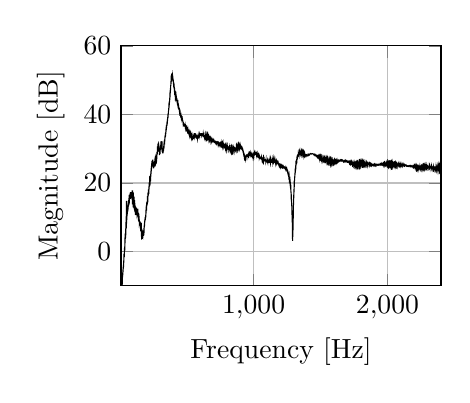
\begin{tikzpicture}

\begin{axis}[%
width=1.6in,
height=1.2in,
at={(1.011in,0.642in)},
scale only axis,
xmin=10,
xmax=2400,
xmajorgrids,
ymin=-10,
ymax=60,
ymajorgrids,
ylabel={Magnitude [dB]},
xlabel={Frequency [Hz]},
axis background/.style={fill=white}
]
\addplot [color=black,solid,forget plot]
  table[row sep=crcr]{%
0	-16.9279009965362\\
0.666675926054529	-21.4183411326356\\
1.33335185210906	-15.3081787642989\\
2.00002777816359	-38.2506326236054\\
2.66670370421811	-8.13933185731465\\
3.33337963027264	-4.56532991367051\\
4.00005555632717	-8.6450221628849\\
4.6667314823817	-11.4444253353331\\
5.33340740843623	-8.77855138258987\\
6.00008333449076	-23.0042660448919\\
6.66675926054529	-15.4904253871871\\
7.33343518659981	-16.0717555634094\\
8.00011111265434	-23.1213112704057\\
8.66678703870887	-25.1712608953541\\
9.3334629647634	-14.5015100526572\\
10.0001388908179	-15.1329736780436\\
10.6668148168725	-33.5222215736596\\
11.333490742927	-44.2849740783617\\
12.0001666689815	-37.2425777758977\\
12.666842595036	-16.8794008482717\\
13.3335185210906	-18.2813358397719\\
14.0001944471451	-12.6177398821699\\
14.6668703731996	-13.1256047551704\\
15.3335462992542	-12.7011284518986\\
16.0002222253087	-16.0967061156175\\
16.6668981513632	-11.9393825828523\\
17.3335740774177	-11.5323374773233\\
18.0002500034723	-9.55819091049596\\
18.6669259295268	-9.82533226319535\\
19.3336018555813	-7.89618462078667\\
20.0002777816359	-7.41922583813186\\
20.6669537076904	-7.47106784389362\\
21.3336296337449	-6.27008516674282\\
22.0003055597994	-6.52284310387436\\
22.666981485854	-6.19575537673559\\
23.3336574119085	-6.84980897855785\\
24.000333337963	-5.95864918955186\\
24.6670092640176	-5.9006816659805\\
25.3336851900721	-5.00931528764057\\
26.0003611161266	-4.53057524598824\\
26.6670370421811	-4.94907989897713\\
27.3337129682357	-4.08711111607078\\
28.0003888942902	-3.83024125322941\\
28.6670648203447	-4.52992181097497\\
29.3337407463993	-3.6502692211478\\
30.0004166724538	-3.20618988374658\\
30.6670925985083	-2.80000788307063\\
31.3337685245628	-1.52518433811382\\
32.0004444506174	-0.672028198145344\\
32.6671203766719	-1.15479878077497\\
33.3337963027264	-1.68531657561136\\
34.000472228781	-1.4451534495138\\
34.6671481548355	-0.259973892663675\\
35.33382408089	0.44705736328146\\
36.0005000069445	0.932899270152305\\
36.6671759329991	0.964993361692336\\
37.3338518590536	0.221429595109325\\
38.0005277851081	0.976286067389284\\
38.6672037111627	2.251906853355\\
39.3338796372172	3.11342101657123\\
40.0005555632717	3.03515954820957\\
40.6672314893262	2.4519719381298\\
41.3339074153808	4.1604549942023\\
42.0005833414353	5.31504068496769\\
42.6672592674898	5.11989872257474\\
43.3339351935444	3.95342409471588\\
44.0006111195989	5.09806585668475\\
44.6672870456534	6.64099599177079\\
45.3339629717079	6.19075767459398\\
46.0006388977625	4.78420948614496\\
46.667314823817	6.9472075706461\\
47.3339907498715	8.54967071376283\\
48.0006666759261	7.0514697773129\\
48.6673426019806	6.74997481901935\\
49.3340185280351	9.58613894321484\\
50.0006944540896	14.7381552738682\\
50.6673703801442	8.13924458755057\\
51.3340463061987	9.40492939540913\\
52.0007222322532	10.5707333882724\\
52.6673981583078	9.22506884658579\\
53.3340740843623	9.78524957610559\\
54.0007500104168	11.55298143967\\
54.6674259364713	10.7265233822035\\
55.3341018625259	10.3092911794162\\
56.0007777885804	11.8347015966299\\
56.6674537146349	11.8067407838707\\
57.3341296406895	10.9476249627983\\
58.000805566744	12.3407870387018\\
58.6674814927985	12.7663562104367\\
59.334157418853	11.5811876473992\\
60.0008333449076	12.9482238400978\\
60.6675092709621	13.5156679561678\\
61.3341851970166	11.7722376081832\\
62.0008611230712	13.9701775771694\\
62.6675370491257	13.8254081919018\\
63.3342129751802	12.2867180721075\\
64.0008889012347	14.6779783560284\\
64.6675648272893	13.8197069557275\\
65.3342407533438	13.6236198325594\\
66.0009166793983	14.794514788441\\
66.6675926054529	13.8884094279113\\
67.3342685315074	14.5473945849119\\
68.0009444575619	14.9629138699167\\
68.6676203836164	13.9676874170743\\
69.334296309671	15.5649234144142\\
70.0009722357255	14.7387564774492\\
70.66764816178	14.6354705382749\\
71.3343240878346	16.5165337889125\\
72.0010000138891	14.1379045280302\\
72.6676759399436	16.2704176944307\\
73.3343518659981	15.4550834235895\\
74.0010277920527	15.5654495732574\\
74.6677037181072	16.1182830018597\\
75.3343796441617	15.4493843425366\\
76.0010555702163	16.6343827796093\\
76.6677314962708	15.2813603062876\\
77.3344074223253	16.5941179741883\\
78.0010833483798	16.3938062899021\\
78.6677592744344	15.6497186915841\\
79.3344352004889	17.2118566121765\\
80.0011111265434	15.3749357059223\\
80.667787052598	17.2281234645334\\
81.3344629786525	15.5527780655591\\
82.001138904707	17.2944941549144\\
82.6678148307615	15.5105605795263\\
83.3344907568161	17.3295239611793\\
84.0011666828706	15.9857913235393\\
84.6678426089251	16.9962753990301\\
85.3345185349797	16.5437000017898\\
86.0011944610342	16.892048281255\\
86.6678703870887	16.6188535705749\\
87.3345463131432	17.125120403957\\
88.0012222391978	16.5664359900114\\
88.6678981652523	17.2373719131278\\
89.3345740913068	16.6097895452819\\
90.0012500173614	17.2017104629694\\
90.6679259434159	16.3505093357087\\
91.3346018694704	17.1009540937067\\
92.0012777955249	15.9564934479412\\
92.6679537215795	17.2243412053367\\
93.334629647634	15.062865056471\\
94.0013055736885	17.8530961717229\\
94.667981499743	13.7565683063786\\
95.3346574257976	17.8196464739369\\
96.0013333518521	14.3171585367597\\
96.6680092779066	16.8226101687816\\
97.3346852039612	15.1626941139365\\
98.0013611300157	16.4550987007153\\
98.6680370560702	15.2321034507723\\
99.3347129821248	15.5528850282962\\
100.001388908179	17.2643318495352\\
100.668064834234	12.882340722427\\
101.334740760288	17.2082648672373\\
102.001416686343	13.7735494851163\\
102.668092612397	15.4755427042953\\
103.334768538452	15.8001731921223\\
104.001444464506	13.6873474043166\\
104.668120390561	15.6094245140996\\
105.334796316616	13.5460375553814\\
106.00147224267	15.6140950561703\\
106.668148168725	14.6183844546593\\
107.334824094779	12.5991581172947\\
108.001500020834	16.0033893642304\\
108.668175946888	13.6499416023787\\
109.334851872943	13.4129960357908\\
110.001527798997	14.4558360095099\\
110.668203725052	12.1952467747455\\
111.334879651106	14.9688294566925\\
112.001555577161	13.4875698403119\\
112.668231503215	11.9156581170656\\
113.33490742927	14.1379846606405\\
114.001583355324	13.3986941979772\\
114.668259281379	11.4928273524885\\
115.334935207433	12.9139725182134\\
116.001611133488	12.3582777625134\\
116.668287059542	13.1506557752826\\
117.334962985597	12.9857538562088\\
118.001638911652	10.7207545661721\\
118.668314837706	10.9764238262849\\
119.334990763761	13.0687892032026\\
120.001666689815	12.729752409596\\
120.66834261587	11.8578973892742\\
121.335018541924	10.8755275171025\\
122.001694467979	10.6327266863738\\
122.668370394033	11.3607268636494\\
123.335046320088	12.7255708158878\\
124.001722246142	12.5774689354413\\
124.668398172197	12.5712217560303\\
125.335074098251	12.0213688110301\\
126.001750024306	11.7421252591609\\
126.66842595036	10.9726159707938\\
127.335101876415	11.8567249296978\\
128.001777802469	12.0679856958511\\
128.668453728524	12.4245368450789\\
129.335129654579	11.8731999166577\\
130.001805580633	11.5093276023123\\
130.668481506688	10.7497090368455\\
131.335157432742	10.8742630322477\\
132.001833358797	11.3420692927744\\
132.668509284851	11.9324535486958\\
133.335185210906	12.4890322383224\\
134.00186113696	12.1588170660838\\
134.668537063015	12.1865399108146\\
135.335212989069	11.3408641365805\\
136.001888915124	11.3969376123334\\
136.668564841178	11.0352821971076\\
137.335240767233	10.9444003187438\\
138.001916693287	10.8738083213454\\
138.668592619342	10.2956373935549\\
139.335268545396	10.8488637109948\\
140.001944471451	10.1158918276437\\
140.668620397506	10.2567663682963\\
141.33529632356	9.99873986182217\\
142.001972249615	10.0693149460955\\
142.668648175669	10.8216619924352\\
143.335324101724	10.0636475831137\\
144.002000027778	10.1473968307612\\
144.668675953833	9.37176901804372\\
145.335351879887	8.82189716291272\\
146.002027805942	9.26890697293256\\
146.668703731996	8.37933249639471\\
147.335379658051	8.5129949478647\\
148.002055584105	8.25664809188938\\
148.66873151016	7.59546154999731\\
149.335407436214	8.63646349643308\\
150.002083362269	7.72957770700453\\
150.668759288323	8.12361515757583\\
151.335435214378	8.76975833201154\\
152.002111140433	7.60624001168165\\
152.668787066487	7.90615265214705\\
153.335462992542	8.52306017769451\\
154.002138918596	7.72359568589949\\
154.668814844651	8.43393868139944\\
155.335490770705	8.12492313841903\\
156.00216669676	6.15421961097034\\
156.668842622814	6.17111428583323\\
157.335518548869	6.78929536061995\\
158.002194474923	6.54543650135756\\
158.668870400978	8.15317594874093\\
159.335546327032	8.4404611524193\\
160.002222253087	7.13058830912283\\
160.668898179141	7.69216527389577\\
161.335574105196	8.25487753517335\\
162.00225003125	6.7034313110272\\
162.668925957305	5.47691768130689\\
163.335601883359	4.32462316409292\\
164.002277809414	3.48363823282886\\
164.668953735469	4.81239049565484\\
165.335629661523	6.63481177110289\\
166.002305587578	5.54674955693595\\
166.668981513632	3.71946479387339\\
167.335657439687	4.84372524326339\\
168.002333365741	5.8747413796306\\
168.669009291796	4.47260382471733\\
169.33568521785	4.12862397542525\\
170.002361143905	5.87831168479071\\
170.669037069959	6.19369723707532\\
171.335712996014	5.12138757273387\\
172.002388922068	5.12950301858558\\
172.669064848123	5.10389050081878\\
173.335740774177	4.93628451197116\\
174.002416700232	5.36362476075035\\
174.669092626286	6.01671560773166\\
175.335768552341	5.09245658754945\\
176.002444478396	4.56755117797211\\
176.66912040445	5.09328708769413\\
177.335796330505	5.45211316436213\\
178.002472256559	5.77777543488704\\
178.669148182614	5.24480644466215\\
179.335824108668	4.69044590399565\\
180.002500034723	5.84783985837483\\
180.669175960777	6.79816017901104\\
181.335851886832	6.12920254424728\\
182.002527812886	5.40888960746684\\
182.669203738941	6.55715680024164\\
183.335879664995	7.58505756064407\\
184.00255559105	7.42618125722052\\
184.669231517104	7.06794027093493\\
185.335907443159	7.89875504650835\\
186.002583369213	8.46653409368815\\
186.669259295268	8.45619996867247\\
187.335935221323	8.87641890413148\\
188.002611147377	9.15075599864213\\
188.669287073432	9.47713295721075\\
189.335962999486	9.11837493367218\\
190.002638925541	9.60690823350438\\
190.669314851595	10.0877069176776\\
191.33599077765	9.34596575575194\\
192.002666703704	9.17433101619092\\
192.669342629759	9.95883045225337\\
193.336018555813	9.78642534176494\\
194.002694481868	9.78960737403864\\
194.669370407922	10.4430233901125\\
195.336046333977	10.869446570475\\
196.002722260031	10.8972027507492\\
196.669398186086	12.0272143550404\\
197.33607411214	12.3616054617798\\
198.002750038195	12.2366835979818\\
198.66942596425	12.4896886593903\\
199.336101890304	11.9201349410639\\
200.002777816359	12.2219112258103\\
200.669453742413	11.9519937536338\\
201.336129668468	13.1008667951234\\
202.002805594522	13.3467578176828\\
202.669481520577	14.5116182002635\\
203.336157446631	14.283895454482\\
204.002833372686	14.133957118903\\
204.66950929874	13.53893367871\\
205.336185224795	13.7872710932936\\
206.002861150849	14.030377875297\\
206.669537076904	15.4203508400866\\
207.336213002958	15.7160778024656\\
208.002888929013	16.1213096328429\\
208.669564855067	15.0953023500134\\
209.336240781122	15.1175686686582\\
210.002916707176	15.0574858305489\\
210.669592633231	16.3551922504888\\
211.336268559286	16.7465716449223\\
212.00294448534	17.227034909442\\
212.669620411395	16.1114584486006\\
213.336296337449	16.7170763385365\\
214.002972263504	17.2077990370438\\
214.669648189558	18.1547304851792\\
215.336324115613	17.8059067767985\\
216.003000041667	16.9567063357973\\
216.669675967722	16.7865430844668\\
217.336351893776	17.776104104953\\
218.003027819831	19.0253583483322\\
218.669703745885	18.4120989003021\\
219.33637967194	18.1080152784189\\
220.003055597994	18.7192377561787\\
220.669731524049	19.8569502475578\\
221.336407450103	20.1311253372346\\
222.003083376158	18.9241930575534\\
222.669759302213	19.1143834712985\\
223.336435228267	20.410956744549\\
224.003111154322	20.2782185796046\\
224.669787080376	19.4137368671917\\
225.336463006431	19.2306964289234\\
226.003138932485	20.8986277236272\\
226.66981485854	20.8044757533223\\
227.336490784594	19.4879190743691\\
228.003166710649	20.7227182101529\\
228.669842636703	21.9996320980121\\
229.336518562758	20.989209355655\\
230.003194488812	20.9552396149809\\
230.669870414867	22.619308328675\\
231.336546340921	22.4294638899481\\
232.003222266976	21.864827615083\\
232.66989819303	22.9362616662781\\
233.336574119085	23.5514183739824\\
234.00325004514	22.645223372233\\
234.669925971194	23.3585154812955\\
235.336601897249	24.3127933853688\\
236.003277823303	23.607183968095\\
236.669953749358	23.7238579263005\\
237.336629675412	25.0025452544358\\
238.003305601467	24.3663577552105\\
238.669981527521	24.3738219128797\\
239.336657453576	25.7114023550483\\
240.00333337963	24.8230561399097\\
240.670009305685	24.8516747973741\\
241.336685231739	26.3277069392566\\
242.003361157794	25.4865286352322\\
242.670037083848	25.6970512757761\\
243.336713009903	26.2752329968005\\
244.003388935957	25.5394347351492\\
244.670064862012	26.5136325873372\\
245.336740788066	26.5283719196591\\
246.003416714121	25.6538438197739\\
246.670092640176	26.8095813975763\\
247.33676856623	25.9760613024417\\
248.003444492285	26.0211609098702\\
248.670120418339	26.257578852557\\
249.336796344394	25.1760575786441\\
250.003472270448	26.0558723070739\\
250.670148196503	24.9643043507858\\
251.336824122557	24.9545951432918\\
252.003500048612	24.7502996941155\\
252.670175974666	24.2502249664317\\
253.336851900721	25.1465701580961\\
254.003527826775	24.654893428422\\
254.67020375283	25.5695206841929\\
255.336879678884	25.1520865145633\\
256.003555604939	25.4747474658713\\
256.670231530993	25.3983075013297\\
257.336907457048	25.2388037537479\\
258.003583383103	25.3828157983144\\
258.670259309157	24.872229832802\\
259.336935235212	25.1600487006331\\
260.003611161266	24.8029499908593\\
260.670287087321	25.2618539495279\\
261.336963013375	25.4431634714335\\
262.00363893943	26.2579536068526\\
262.670314865484	26.4149215190718\\
263.336990791539	27.1048388530225\\
264.003666717593	26.88577446931\\
264.670342643648	27.0603670741736\\
265.337018569702	26.5966238215382\\
266.003694495757	26.3987783488505\\
266.670370421811	25.8440537875868\\
267.337046347866	26.3745700369699\\
268.00372227392	26.3275671379394\\
268.670398199975	26.9809549676923\\
269.33707412603	26.9179326734232\\
270.003750052084	27.031061824242\\
270.670425978139	26.0930897661419\\
271.337101904193	26.2068477746243\\
272.003777830248	25.7720169669728\\
272.670453756302	26.4193847225641\\
273.337129682357	26.5924955985323\\
274.003805608411	27.4860320647263\\
274.670481534466	27.2640722318228\\
275.33715746052	27.0273713198996\\
276.003833386575	26.8454514171583\\
276.670509312629	27.128398897063\\
277.337185238684	28.0227717976803\\
278.003861164738	28.1836384021408\\
278.670537090793	29.0532734083002\\
279.337213016847	28.6517082639762\\
280.003888942902	28.7902124081496\\
280.670564868956	28.3604756178846\\
281.337240795011	29.0843619912607\\
282.003916721066	29.9319750613908\\
282.67059264712	29.8686114619573\\
283.337268573175	29.9353609768545\\
284.003944499229	29.1468469310427\\
284.670620425284	30.0803362076434\\
285.337296351338	30.8420224296377\\
286.003972277393	31.2081047979354\\
286.670648203447	31.286937808188\\
287.337324129502	30.1501606267459\\
288.004000055556	30.6325059209878\\
288.670675981611	31.2882523300911\\
289.337351907665	31.5495814666346\\
290.00402783372	31.5555583764569\\
290.670703759774	30.1800557882294\\
291.337379685829	30.3580238006857\\
292.004055611883	31.179193779535\\
292.670731537938	30.642347624963\\
293.337407463993	30.1923297874347\\
294.004083390047	29.5186272870957\\
294.670759316102	29.5534286234126\\
295.337435242156	30.1465669162635\\
296.004111168211	28.9814217713933\\
296.670787094265	28.1498292532542\\
297.33746302032	29.4088223731069\\
298.004138946374	29.3245089835723\\
298.670814872429	28.3222377824069\\
299.337490798483	28.5909500593694\\
300.004166724538	29.2008846292547\\
300.670842650592	29.2993250952738\\
301.337518576647	29.181255624727\\
302.004194502701	29.1232705184969\\
302.670870428756	29.7695151410371\\
303.33754635481	30.3311977834594\\
304.004222280865	29.7588545412841\\
304.67089820692	29.7586169571078\\
305.337574132974	30.9614951494651\\
306.004250059029	30.9908352706764\\
306.670925985083	30.1758337913558\\
307.337601911138	31.0800686137851\\
308.004277837192	32.0440886312034\\
308.670953763247	31.1975510393113\\
309.337629689301	31.1153643319194\\
310.004305615356	32.1541637247916\\
310.67098154141	31.9704353846474\\
311.337657467465	31.0564297587083\\
312.004333393519	31.5920487527022\\
312.671009319574	31.623500671551\\
313.337685245628	30.7271460878498\\
314.004361171683	31.0858512775447\\
314.671037097737	30.5915097534758\\
315.337713023792	29.8500284472723\\
316.004388949847	30.4604063565437\\
316.671064875901	30.5995879496596\\
317.337740801956	28.9957421770608\\
318.00441672801	29.3224832873808\\
318.671092654065	30.1410876006405\\
319.337768580119	28.9620164406353\\
320.004444506174	29.3576342762982\\
320.671120432228	29.406891482078\\
321.337796358283	28.6232910312712\\
322.004472284337	29.6206109562625\\
322.671148210392	29.6846292256823\\
323.337824136446	28.7201618603733\\
324.004500062501	29.4064652237257\\
324.671175988555	29.5323549428459\\
325.33785191461	29.233500314125\\
326.004527840664	30.2474053680003\\
326.671203766719	29.6185809635727\\
327.337879692774	29.4155634210418\\
328.004555618828	30.2393887578561\\
328.671231544883	29.9206576119773\\
329.337907470937	30.6036765035739\\
330.004583396992	31.1239749147597\\
330.671259323046	30.3117781995547\\
331.337935249101	31.4444095096102\\
332.004611175155	30.9702867158024\\
332.67128710121	31.4190188296927\\
333.337963027264	32.209443891953\\
334.004638953319	31.4909390154688\\
334.671314879373	32.5399690365598\\
335.337990805428	32.0610147855211\\
336.004666731482	31.9927156766263\\
336.671342657537	32.7311092662876\\
337.338018583591	32.1562495404516\\
338.004694509646	33.5844284426966\\
338.671370435701	33.0813467840194\\
339.338046361755	33.5932717630556\\
340.00472228781	33.9538114063728\\
340.671398213864	33.4658344591896\\
341.338074139919	34.2640656181199\\
342.004750065973	33.6026398933603\\
342.671425992028	34.7479570247904\\
343.338101918082	34.0904860148513\\
344.004777844137	34.650185833305\\
344.671453770191	34.8220438698089\\
345.338129696246	34.6679395955606\\
346.0048056223	35.770451101566\\
346.671481548355	35.2119435786536\\
347.338157474409	36.3855133439958\\
348.004833400464	35.494789642862\\
348.671509326518	36.50119120047\\
349.338185252573	36.029130982356\\
350.004861178627	36.930871811582\\
350.671537104682	36.5919966038214\\
351.338213030737	36.8533732302767\\
352.004888956791	36.9307957247168\\
352.671564882846	37.142637828836\\
353.3382408089	37.4474149705182\\
354.004916734955	37.3884634774258\\
354.671592661009	37.9157746943661\\
355.338268587064	37.3394500379921\\
356.004944513118	38.5112362023068\\
356.671620439173	38.050669602629\\
357.338296365227	38.6277881321766\\
358.004972291282	38.2813889179649\\
358.671648217336	39.1582968323552\\
359.338324143391	38.8400917400509\\
360.005000069445	39.5120233669218\\
360.6716759955	39.0801052595019\\
361.338351921554	40.1907243951241\\
362.005027847609	39.6077257920886\\
362.671703773664	40.3960143273025\\
363.338379699718	40.1996278939594\\
364.005055625773	40.9252636214818\\
364.671731551827	40.9420451669278\\
365.338407477882	41.132421354435\\
366.005083403936	41.79524924421\\
366.671759329991	41.385466997776\\
367.338435256045	42.4261568679765\\
368.0051111821	41.9450176048338\\
368.671787108154	43.2121705535546\\
369.338463034209	42.1492923666708\\
370.005138960263	43.6285883226348\\
370.671814886318	42.7247107142783\\
371.338490812372	43.7752940492817\\
372.005166738427	43.5023989854252\\
372.671842664481	44.0631066643358\\
373.338518590536	44.1981815840344\\
374.005194516591	44.378966798559\\
374.671870442645	45.2447394900619\\
375.3385463687	44.9698847191265\\
376.005222294754	46.0444406022955\\
376.671898220809	46.0033113710992\\
377.338574146863	46.2062727051692\\
378.005250072918	46.9776539191969\\
378.671925998972	46.2476399915643\\
379.338601925027	47.6566249304577\\
380.005277851081	46.9757533395599\\
380.671953777136	48.1232641231698\\
381.33862970319	48.4752980246366\\
382.005305629245	48.5197040033995\\
382.671981555299	49.688664218396\\
383.338657481354	48.9273040829867\\
384.005333407408	50.0043644096501\\
384.672009333463	49.8889767867692\\
385.338685259517	49.9645423950812\\
386.005361185572	51.0440536238953\\
386.672037111627	50.5289060131485\\
387.338713037681	51.3383431552267\\
388.005388963736	51.2839821628946\\
388.67206488979	50.8419322105441\\
389.338740815845	51.7463781399043\\
390.005416741899	51.2164681525086\\
390.672092667954	51.6486603341978\\
391.338768594008	51.8632954289134\\
392.005444520063	51.1179626962237\\
392.672120446117	51.2671825962871\\
393.338796372172	51.5096059041523\\
394.005472298226	51.1212174497222\\
394.672148224281	51.3778305767553\\
395.338824150335	51.1445871684515\\
396.00550007639	50.3985426579409\\
396.672176002444	51.0330998891381\\
397.338851928499	50.861864902441\\
398.005527854554	50.2149251107341\\
398.672203780608	50.266644298128\\
399.338879706663	50.1972626317929\\
400.005555632717	49.6650101875795\\
400.672231558772	50.0673137859406\\
401.338907484826	49.5852031027568\\
402.005583410881	48.777833684622\\
402.672259336935	49.3545517887215\\
403.33893526299	49.2859928595329\\
404.005611189044	48.196633634248\\
404.672287115099	48.2003612004414\\
405.338963041153	48.9027869476051\\
406.005638967208	47.7650357389536\\
406.672314893262	47.3632460550763\\
407.338990819317	47.956013512881\\
408.005666745371	47.8025522613278\\
408.672342671426	46.5158950816167\\
409.339018597481	46.9557682959702\\
410.005694523535	47.6815132241608\\
410.67237044959	46.4820378807706\\
411.339046375644	45.7239023312394\\
412.005722301699	46.5729562183314\\
412.672398227753	46.9871331182384\\
413.339074153808	45.7331416982325\\
414.005750079862	45.2080821621431\\
414.672426005917	46.1967219855158\\
415.339101931971	45.9474407572013\\
416.005777858026	45.2619310983116\\
416.67245378408	45.3983816911296\\
417.339129710135	45.5475974568235\\
418.005805636189	45.274310445586\\
418.672481562244	45.0103024170366\\
419.339157488298	45.2234151266298\\
420.005833414353	45.3777014081454\\
420.672509340407	44.9394259764528\\
421.339185266462	44.3211607317826\\
422.005861192517	44.6399844487932\\
422.672537118571	45.2341580409637\\
423.339213044626	45.082392989654\\
424.00588897068	44.3598389672571\\
424.672564896735	43.94602747172\\
425.339240822789	44.3079838450371\\
426.005916748844	44.8361095675557\\
426.672592674898	44.3366937739764\\
427.339268600953	43.7572939827699\\
428.005944527007	44.1312633020826\\
428.672620453062	44.1286130009636\\
429.339296379116	44.0441453174559\\
430.005972305171	43.6448274854075\\
430.672648231225	42.8422839278845\\
431.33932415728	43.232058091821\\
432.006000083334	43.7633505631474\\
432.672676009389	43.7999856573777\\
433.339351935444	43.2895968586169\\
434.006027861498	42.7110915814016\\
434.672703787553	42.7344294966279\\
435.339379713607	42.8340162246066\\
436.006055639662	42.9860782017745\\
436.672731565716	42.6943195994617\\
437.339407491771	42.1886221002554\\
438.006083417825	41.733283524386\\
438.67275934388	41.7288734726405\\
439.339435269934	42.2759032480001\\
440.006111195989	42.4067682225549\\
440.672787122043	42.2525906541743\\
441.339463048098	41.6913411526553\\
442.006138974152	41.4278078722772\\
442.672814900207	41.4123562550825\\
443.339490826261	41.5774637233424\\
444.006166752316	41.7715583786801\\
444.672842678371	41.7232932339832\\
445.339518604425	41.6173508832711\\
446.00619453048	41.205663523993\\
446.672870456534	40.8087635199175\\
447.339546382589	40.6046424864804\\
448.006222308643	40.7448079649313\\
448.672898234698	41.0690564503679\\
449.339574160752	41.2181108063511\\
450.006250086807	41.1314413500924\\
450.672926012861	40.7395276738148\\
451.339601938916	40.4669577160497\\
452.00627786497	40.0799419463443\\
452.672953791025	39.9847339412889\\
453.339629717079	39.8448911381275\\
454.006305643134	40.0165030085632\\
454.672981569188	39.9839789316189\\
455.339657495243	40.1619561944374\\
456.006333421298	40.1190934656066\\
456.673009347352	40.1495139889202\\
457.339685273407	39.8850430179133\\
458.006361199461	39.5887666839898\\
458.673037125516	39.3862286665865\\
459.33971305157	39.1832182637346\\
460.006388977625	39.0909272868139\\
460.673064903679	38.8362673277947\\
461.339740829734	38.9937901136302\\
462.006416755788	38.9613386752908\\
462.673092681843	39.1484367283641\\
463.339768607897	39.2105246709853\\
464.006444533952	39.1082564431141\\
464.673120460006	39.235955415828\\
465.339796386061	39.1974398681973\\
466.006472312115	39.2221275642854\\
466.67314823817	39.0330779878723\\
467.339824164225	38.8971479423561\\
468.006500090279	38.8268418022667\\
468.673176016334	38.4956602117531\\
469.339851942388	38.3082203718619\\
470.006527868443	38.11285153749\\
470.673203794497	38.0390395514909\\
471.339879720552	38.0445055689608\\
472.006555646606	37.7642039793024\\
472.673231572661	37.7438480914986\\
473.339907498715	37.6669692445931\\
474.00658342477	37.3680920150366\\
474.673259350824	37.4906291542461\\
475.339935276879	37.5125090093773\\
476.006611202933	37.312260265163\\
476.673287128988	37.2284482190944\\
477.339963055042	37.1778207254047\\
478.006638981097	37.0720464914928\\
478.673314907152	37.1891687289698\\
479.339990833206	37.1473327877027\\
480.006666759261	36.7785225703585\\
480.673342685315	36.9988115870951\\
481.34001861137	36.949660503137\\
482.006694537424	36.8115392877671\\
482.673370463479	36.8049403786455\\
483.340046389533	36.7427760879646\\
484.006722315588	36.775106489845\\
484.673398241642	36.7989686544739\\
485.340074167697	36.7340153103329\\
486.006750093751	36.7939046891369\\
486.673426019806	36.7992100113478\\
487.34010194586	36.9354981785788\\
488.006777871915	37.0309344575397\\
488.673453797969	36.8086832206762\\
489.340129724024	36.9756747016256\\
490.006805650078	36.9491779866781\\
490.673481576133	36.9538179665148\\
491.340157502188	36.8154522099347\\
492.006833428242	36.6988787240293\\
492.673509354297	36.5891062363041\\
493.340185280351	36.1700168157973\\
494.006861206406	36.0782398224392\\
494.67353713246	35.7025003736008\\
495.340213058515	35.7891761464779\\
496.006888984569	35.691000836196\\
496.673564910624	35.9111910801841\\
497.340240836678	35.8498684699018\\
498.006916762733	36.141625351312\\
498.673592688787	36.238056360328\\
499.340268614842	36.1142932342614\\
500.006944540896	36.074836549324\\
500.673620466951	35.875520509788\\
501.340296393005	35.7288084431858\\
502.00697231906	35.6299176597298\\
502.673648245115	35.2939626999772\\
503.340324171169	35.2491304016411\\
504.007000097224	35.2344659713657\\
504.673676023278	35.5291485113291\\
505.340351949333	35.774654741276\\
506.007027875387	35.8419733622346\\
506.673703801442	35.6300231149903\\
507.340379727496	35.4061028290424\\
508.007055653551	34.8669730978448\\
508.673731579605	34.9103088667212\\
509.34040750566	34.9499224493508\\
510.007083431714	35.1340503891664\\
510.673759357769	35.46220996679\\
511.340435283823	35.2937141260507\\
512.007111209878	35.2004060316806\\
512.673787135932	34.8873010979635\\
513.340463061987	34.6246499853537\\
514.007138988041	34.5546555239614\\
514.673814914096	34.8817401000586\\
515.340490840151	35.2381163902642\\
516.007166766205	35.0099218705068\\
516.67384269226	34.8108710160208\\
517.340518618314	34.3918849876274\\
518.007194544369	34.2976139085778\\
518.673870470423	34.5685289956903\\
519.340546396478	34.9186032929833\\
520.007222322532	34.8643371659941\\
520.673898248587	34.5256413606186\\
521.340574174641	34.0927817852128\\
522.007250100696	34.2365231083242\\
522.67392602675	34.5788356799019\\
523.340601952805	34.7363593899077\\
524.007277878859	34.5077627186895\\
524.673953804914	34.1712774400521\\
525.340629730968	34.056154064716\\
526.007305657023	34.4018319080599\\
526.673981583078	34.5595148842761\\
527.340657509132	34.4384947558035\\
528.007333435187	34.016236602916\\
528.674009361241	33.9426884439341\\
529.340685287296	34.2331835444322\\
530.00736121335	34.4667423861079\\
530.674037139405	34.0953854347935\\
531.340713065459	33.681264115032\\
532.007388991514	33.9002842551104\\
532.674064917568	34.1653539431457\\
533.340740843623	34.0266857012481\\
534.007416769677	33.4591571113749\\
534.674092695732	33.3479612727928\\
535.340768621786	33.9382481898624\\
536.007444547841	33.9875744324611\\
536.674120473896	33.2249208078281\\
537.34079639995	33.0142782017828\\
538.007472326005	33.5059554981659\\
538.674148252059	33.6302486649957\\
539.340824178114	33.1426610102805\\
540.007500104168	32.9195117343711\\
540.674176030223	33.5190748452561\\
541.340851956277	33.453312315093\\
542.007527882332	32.765492171701\\
542.674203808386	32.8277140918065\\
543.340879734441	33.3035405168046\\
544.007555660495	33.1354906093175\\
544.67423158655	32.5963556039216\\
545.340907512604	33.1054903149874\\
546.007583438659	33.5490775697096\\
546.674259364713	32.9275420426627\\
547.340935290768	32.9518663333551\\
548.007611216823	33.5879057874799\\
548.674287142877	33.3999793918109\\
549.340963068932	32.8451579459877\\
550.007638994986	33.4086477421994\\
550.674314921041	33.5055597574142\\
551.340990847095	32.927944997675\\
552.00766677315	33.1685729714068\\
552.674342699204	33.6738323421744\\
553.341018625259	33.1655157523761\\
554.007694551313	33.1395183608941\\
554.674370477368	34.0576993072326\\
555.341046403422	33.3754744132068\\
556.007722329477	33.3301652928771\\
556.674398255531	34.0977171853219\\
557.341074181586	33.5530081058455\\
558.00775010764	33.2881857002199\\
558.674426033695	34.2878702793603\\
559.341101959749	33.529859651547\\
560.007777885804	33.6323561836189\\
560.674453811858	34.5432313224055\\
561.341129737913	33.7691591001552\\
562.007805663968	33.7648313460953\\
562.674481590022	34.4003752083563\\
563.341157516077	33.3195154611835\\
564.007833442131	33.9085513992225\\
564.674509368186	34.2754847427908\\
565.34118529424	33.2226237717665\\
566.007861220295	34.4303140406837\\
566.674537146349	33.8289629964289\\
567.341213072404	33.4016135986858\\
568.007888998458	34.2677833301837\\
568.674564924513	33.308637494383\\
569.341240850567	33.8920609344158\\
570.007916776622	34.1009684000883\\
570.674592702676	33.0116577283507\\
571.341268628731	34.0907749971592\\
572.007944554785	33.2424985884742\\
572.67462048084	33.5932895486204\\
573.341296406895	33.8528584004567\\
574.007972332949	33.038129195683\\
574.674648259004	33.7881084785692\\
575.341324185058	33.0496349220152\\
576.008000111113	33.4593119091023\\
576.674676037167	33.490282600599\\
577.341351963222	32.8013572106633\\
578.008027889276	33.6647117740034\\
578.674703815331	32.8420341005965\\
579.341379741385	33.5700000497351\\
580.00805566744	33.1002419572249\\
580.674731593494	32.967581247062\\
581.341407519549	33.5190895839907\\
582.008083445603	32.7664392427667\\
582.674759371658	33.5119090873245\\
583.341435297712	32.9011927341543\\
584.008111223767	33.3906202663298\\
584.674787149822	33.1386019915591\\
585.341463075876	33.4491188824836\\
586.008139001931	33.3428818007293\\
586.674814927985	33.3154569146741\\
587.34149085404	33.4918910892388\\
588.008166780094	33.0799722913221\\
588.674842706149	33.7310094416265\\
589.341518632203	33.230735943334\\
590.008194558258	33.8699885945028\\
590.674870484312	33.2194073750597\\
591.341546410367	34.0119305993128\\
592.008222336421	33.2661224030276\\
592.674898262476	33.936299708947\\
593.34157418853	33.5286092652608\\
594.008250114585	34.0142689472949\\
594.674926040639	33.5964952693556\\
595.341601966694	34.0974353403564\\
596.008277892749	33.7544744263062\\
596.674953818803	34.011602832284\\
597.341629744858	33.8621015187485\\
598.008305670912	34.1804538522693\\
598.674981596967	33.8302273772866\\
599.341657523021	34.1983448827386\\
600.008333449076	33.9738034069781\\
600.67500937513	34.3204817930506\\
601.341685301185	33.892670218953\\
602.008361227239	34.3805139183459\\
602.675037153294	33.95419501426\\
603.341713079348	34.486957478994\\
604.008389005403	33.7450165263762\\
604.675064931457	34.4540540030191\\
605.341740857512	34.0204010287038\\
606.008416783566	34.5307862916034\\
606.675092709621	33.9493385759033\\
607.341768635676	34.5037698687624\\
608.00844456173	34.0160926408552\\
608.675120487785	34.4329319721613\\
609.341796413839	34.2293195035545\\
610.008472339894	34.1363097984197\\
610.675148265948	34.4872112022698\\
611.341824192003	33.9067497944298\\
612.008500118057	34.5197983136025\\
612.675176044112	33.8094581107522\\
613.341851970166	34.5237384699029\\
614.008527896221	34.0685134611261\\
614.675203822275	34.1808334200345\\
615.34187974833	34.4067337203098\\
616.008555674384	33.9624764582487\\
616.675231600439	34.4586651407507\\
617.341907526493	33.8037321095513\\
618.008583452548	34.3145116899819\\
618.675259378603	34.0796950239667\\
619.341935304657	34.0226666250973\\
620.008611230711	34.4661906176487\\
620.675287156766	33.759552565812\\
621.341963082821	34.3151171772704\\
622.008639008875	33.9107663313782\\
622.67531493493	33.8561685858892\\
623.341990860984	34.2065254198522\\
624.008666787039	33.6957620819054\\
624.675342713093	34.1219612296388\\
625.342018639148	33.9470439106356\\
626.008694565202	33.6517357745443\\
626.675370491257	34.0980685735369\\
627.342046417311	33.6621191856154\\
628.008722343366	33.8693770511988\\
628.67539826942	33.94513307981\\
629.342074195475	33.5468725816838\\
630.008750121529	33.9009531971485\\
630.675426047584	33.8253223588356\\
631.342101973638	33.4855134157708\\
632.008777899693	33.9474383576724\\
632.675453825748	33.5453257128822\\
633.342129751802	33.5812763080841\\
634.008805677857	33.9257734645552\\
634.675481603911	33.429544272674\\
635.342157529966	33.5647768223632\\
636.00883345602	33.8948897383385\\
636.675509382075	33.4694134975685\\
637.342185308129	33.5181094957026\\
638.008861234184	33.8899263043451\\
638.675537160238	33.4969320588819\\
639.342213086293	33.5657607220014\\
640.008889012347	33.8716790032155\\
640.675564938402	33.481117033843\\
641.342240864456	33.6407341030622\\
642.008916790511	33.8756072408629\\
642.675592716565	33.6439938521602\\
643.34226864262	33.5573607359771\\
644.008944568675	33.9252720204089\\
644.675620494729	33.7787193503587\\
645.342296420784	33.5157106374679\\
646.008972346838	33.8228778097862\\
646.675648272893	33.9406708216349\\
647.342324198947	33.4943336647152\\
648.009000125002	33.6742426608352\\
648.675676051056	33.9836269020925\\
649.342351977111	33.6904736005537\\
650.009027903165	33.3597950624708\\
650.67570382922	33.8589189018454\\
651.342379755274	33.9003458600635\\
652.009055681329	33.4066012349979\\
652.675731607383	33.535760428304\\
653.342407533438	33.9033366356792\\
654.009083459492	33.68146962209\\
654.675759385547	33.3192579021166\\
655.342435311602	33.4346217660072\\
656.009111237656	33.7478999358458\\
656.675787163711	33.5815975570917\\
657.342463089765	33.1529148946002\\
658.00913901582	33.4371406539408\\
658.675814941874	33.6944027084794\\
659.342490867929	33.5046767256095\\
660.009166793983	33.1007739282693\\
660.675842720038	33.1756573537547\\
661.342518646092	33.595299017661\\
662.009194572147	33.4511545545507\\
662.675870498201	33.0456524943856\\
663.342546424256	32.9583522818034\\
664.00922235031	33.3670805836277\\
664.675898276365	33.4401758351489\\
665.342574202419	33.1511218817493\\
666.009250128474	32.8382933369558\\
666.675926054529	33.0060261581679\\
667.342601980583	33.4010666284169\\
668.009277906638	33.3148354288899\\
668.675953832692	32.9299717814482\\
669.342629758747	32.6492808497042\\
670.009305684801	32.91851838677\\
670.675981610856	33.1974590568642\\
671.34265753691	33.2500209557731\\
672.009333462965	32.8549835496252\\
672.676009389019	32.6101842860846\\
673.342685315074	32.7425035401326\\
674.009361241128	33.1103374017917\\
674.676037167183	33.1176289889519\\
675.342713093237	33.0229708326858\\
676.009389019292	32.6234836296633\\
676.676064945346	32.5543600999306\\
677.342740871401	32.6144255302425\\
678.009416797456	32.9584905760195\\
678.67609272351	33.0407179797774\\
679.342768649565	32.8358664910016\\
680.009444575619	32.5442882806008\\
680.676120501674	32.3290907680174\\
681.342796427728	32.514003718295\\
682.009472353783	32.6702018407387\\
682.676148279837	32.8692648126594\\
683.342824205892	32.8738260345829\\
684.009500131946	32.6993566414552\\
684.676176058001	32.3878642994136\\
685.342851984055	32.2346787337008\\
686.00952791011	32.4026230527994\\
686.676203836164	32.5157307671085\\
687.342879762219	32.75335657664\\
688.009555688273	32.8523772866013\\
688.676231614328	32.7038430444802\\
689.342907540382	32.5693829666736\\
690.009583466437	32.3326971064929\\
690.676259392492	32.1554502750992\\
691.342935318546	32.1282365233698\\
692.009611244601	32.2447363809181\\
692.676287170655	32.4338369844314\\
693.34296309671	32.5624564249161\\
694.009639022764	32.6933772386892\\
694.676314948819	32.6645121917769\\
695.342990874873	32.5287892523113\\
696.009666800928	32.3779179423651\\
696.676342726982	32.2021206226776\\
697.343018653037	32.0784213629949\\
698.009694579091	32.0031010171002\\
698.676370505146	32.0312781687205\\
699.3430464312	32.1524416542985\\
700.009722357255	32.1438616999946\\
700.676398283309	32.3371180909355\\
701.343074209364	32.5033191539097\\
702.009750135419	32.4945480457803\\
702.676426061473	32.6019341493475\\
703.343101987528	32.5266103026356\\
704.009777913582	32.4944670030076\\
704.676453839637	32.4118127923682\\
705.343129765691	32.3875884752503\\
706.009805691746	32.3321718477217\\
706.6764816178	32.1272171159443\\
707.343157543855	32.12185957597\\
708.009833469909	31.9522591958877\\
708.676509395964	31.9709791856985\\
709.343185322018	31.8703384815312\\
710.009861248073	31.902663566634\\
710.676537174127	31.8322434556239\\
711.343213100182	31.8156341585563\\
712.009889026236	31.8031544507306\\
712.676564952291	31.7952307677142\\
713.343240878346	31.8721265008748\\
714.0099168044	31.8425630176378\\
714.676592730455	31.8460915869806\\
715.343268656509	31.7747773233769\\
716.009944582564	31.8731245099694\\
716.676620508618	31.7872465238707\\
717.343296434673	31.8108261866066\\
718.009972360727	31.7754242366527\\
718.676648286782	31.7754226478886\\
719.343324212836	31.6651993754115\\
720.010000138891	31.7401037267708\\
720.676676064945	31.6968243751771\\
721.343351991	31.6713210668042\\
722.010027917054	31.6392497314606\\
722.676703843109	31.5779774552791\\
723.343379769163	31.6682206233547\\
724.010055695218	31.5560048683367\\
724.676731621273	31.6828010564667\\
725.343407547327	31.6338648442216\\
726.010083473382	31.6897941208052\\
726.676759399436	31.6878850951892\\
727.343435325491	31.7496786766286\\
728.010111251545	31.7979938646607\\
728.6767871776	31.8806826389196\\
729.343463103654	31.9738063890268\\
730.010139029709	31.9497911891209\\
730.676814955763	32.000479518639\\
731.343490881818	31.9761632462102\\
732.010166807872	31.8179592485449\\
732.676842733927	31.7592243004372\\
733.343518659981	31.5280500259099\\
734.010194586036	31.4288452168566\\
734.67687051209	31.2924363914838\\
735.343546438145	31.1327086713359\\
736.0102223642	31.267571097619\\
736.676898290254	31.2724293571764\\
737.343574216309	31.466618088533\\
738.010250142363	31.6328098076416\\
738.676926068418	31.71235516471\\
739.343601994472	31.7685760767256\\
740.010277920527	31.6902572384378\\
740.676953846581	31.4735921864416\\
741.343629772636	31.3527662715309\\
742.01030569869	31.1350025739853\\
742.676981624745	31.0470471592279\\
743.343657550799	31.1869787104551\\
744.010333476854	31.3076934904752\\
744.677009402908	31.4336490085045\\
745.343685328963	31.5957849478195\\
746.010361255017	31.5742269875017\\
746.677037181072	31.3512108070553\\
747.343713107127	31.2604078148425\\
748.010389033181	31.0751370874388\\
748.677064959236	31.0442661561181\\
749.34374088529	31.2185512850864\\
750.010416811345	31.4839078671473\\
750.677092737399	31.5853619514002\\
751.343768663454	31.4832323306125\\
752.010444589508	31.2923850218841\\
752.677120515563	31.0608845372211\\
753.343796441617	30.9858016485648\\
754.010472367672	31.2887358443016\\
754.677148293726	31.554470200435\\
755.343824219781	31.5999856697673\\
756.010500145835	31.3009251477581\\
756.67717607189	31.0392628501075\\
757.343851997944	31.0631745416382\\
758.010527923999	31.2370690297396\\
758.677203850054	31.4358438315693\\
759.343879776108	31.4678333299584\\
760.010555702162	31.290446901575\\
760.677231628217	30.9868561194806\\
761.343907554272	31.0537750512404\\
762.010583480326	31.3654141726845\\
762.677259406381	31.5617261758428\\
763.343935332435	31.3347706742953\\
764.01061125849	30.9447936314721\\
764.677287184544	31.0103078046531\\
765.343963110599	31.3277362698073\\
766.010639036653	31.4587443980989\\
766.677314962708	31.2358898370495\\
767.343990888762	30.9096410999887\\
768.010666814817	31.0863766727689\\
768.677342740871	31.3790987945336\\
769.344018666926	31.2812844191224\\
770.01069459298	30.9801138385729\\
770.677370519035	30.9223009788692\\
771.344046445089	31.1928180765545\\
772.010722371144	31.3504329988772\\
772.677398297199	30.9757374167729\\
773.344074223253	30.8135039856117\\
774.010750149308	31.1216310465479\\
774.677426075362	31.187465009634\\
775.344102001417	30.992236556327\\
776.010777927471	30.8651102411522\\
776.677453853526	30.983358429832\\
777.34412977958	30.9906230222319\\
778.010805705635	30.8086048934886\\
778.677481631689	30.8415981023083\\
779.344157557744	30.9083319970719\\
780.010833483798	30.8755369837037\\
780.677509409853	30.7726318083023\\
781.344185335907	30.8698390902254\\
782.010861261962	30.8123780904449\\
782.677537188016	30.7040105312429\\
783.344213114071	30.8095015906512\\
784.010889040126	30.6833116938033\\
784.67756496618	30.5912630567237\\
785.344240892235	30.6293714945939\\
786.010916818289	30.753420821247\\
786.677592744344	30.5160943537066\\
787.344268670398	30.5310574098844\\
788.010944596453	30.6765714697435\\
788.677620522507	30.5230031978018\\
789.344296448562	30.3431375824294\\
790.010972374616	30.6920577578775\\
790.677648300671	30.4310350101004\\
791.344324226725	30.3249401908681\\
792.01100015278	30.6271221979893\\
792.677676078834	30.4829661390332\\
793.344352004889	30.1738114827838\\
794.011027930943	30.5253782039942\\
794.677703856998	30.4186447153981\\
795.344379783053	30.070768425258\\
796.011055709107	30.5314667974509\\
796.677731635162	30.2562036865482\\
797.344407561216	30.0636874424633\\
798.011083487271	30.4167551003749\\
798.677759413325	30.2150557894816\\
799.34443533938	30.0450217691842\\
800.011111265434	30.4493982441658\\
800.677787191489	30.1155066375975\\
801.344463117543	30.0640223030878\\
802.011139043598	30.4680605362327\\
802.677814969652	29.9423364261177\\
803.344490895707	30.1617294001091\\
804.011166821761	30.3149091814846\\
804.677842747816	29.8441879125702\\
805.34451867387	30.2852927063931\\
806.011194599925	30.1053357242874\\
806.67787052598	29.8846510229053\\
807.344546452034	30.3639573373099\\
808.011222378089	29.841455732038\\
808.677898304143	30.0764389299508\\
809.344574230198	30.1422560742815\\
810.011250156252	29.7283345312\\
810.677926082307	30.2344730005641\\
811.344602008361	29.9486811507882\\
812.011277934416	29.9177252319306\\
812.67795386047	30.1832047778539\\
813.344629786525	29.721049396265\\
814.011305712579	30.1138927635312\\
814.677981638634	29.8187489318162\\
815.344657564688	29.9554105269366\\
816.011333490743	30.0578206729132\\
816.678009416797	29.6468383968274\\
817.344685342852	30.1885943365258\\
818.011361268907	29.672929817619\\
818.678037194961	30.0248265869788\\
819.344713121016	29.8139597264283\\
820.01138904707	29.8452559260585\\
820.678064973125	30.0385218821124\\
821.344740899179	29.6879907516978\\
822.011416825234	30.0597087602783\\
822.678092751288	29.5760750284808\\
823.344768677343	29.9349417942861\\
824.011444603397	29.7333154784904\\
824.678120529452	29.8864767387409\\
825.344796455506	29.8622102943161\\
826.011472381561	29.6712888133454\\
826.678148307615	29.8744007634074\\
827.34482423367	29.6291081354347\\
828.011500159724	29.9430100709118\\
828.678176085779	29.5641176614006\\
829.344852011833	29.9504682703301\\
830.011527937888	29.5942775201492\\
830.678203863943	29.9601173371826\\
831.344879789997	29.5434389693057\\
832.011555716052	29.8896304976387\\
832.678231642106	29.6609318129479\\
833.344907568161	29.852141077877\\
834.011583494215	29.6477264359678\\
834.67825942027	29.8690153621077\\
835.344935346324	29.5633462353248\\
836.011611272379	29.7855400636818\\
836.678287198433	29.6367854308554\\
837.344963124488	29.8063619500842\\
838.011639050542	29.6089385897204\\
838.678314976597	29.8622178337693\\
839.344990902651	29.6426983839055\\
840.011666828706	29.6966881032662\\
840.67834275476	29.5405861098662\\
841.345018680815	29.9138120389953\\
842.01169460687	29.566512978393\\
842.678370532924	29.9379900094613\\
843.345046458979	29.5688502890098\\
844.011722385033	29.904534783417\\
844.678398311088	29.580599611132\\
845.345074237142	29.8269042916205\\
846.011750163197	29.6078289856986\\
846.678426089251	29.8702576342907\\
847.345102015306	29.5353503932067\\
848.01177794136	29.7578231476411\\
848.678453867415	29.8147479382721\\
849.345129793469	29.6623740046643\\
850.011805719524	29.8733261332892\\
850.678481645578	29.610977394411\\
851.345157571633	29.9894510382494\\
852.011833497687	29.6220796839057\\
852.678509423742	29.9100962106483\\
853.345185349797	29.6535443250612\\
854.011861275851	29.7137444142347\\
854.678537201906	29.9071866137343\\
855.34521312796	29.4852289546071\\
856.011889054015	30.0192441696738\\
856.678564980069	29.56886996112\\
857.345240906124	29.935490257007\\
858.011916832178	29.8562236604952\\
858.678592758233	29.665582955785\\
859.345268684287	30.0511905477151\\
860.011944610342	29.642651968654\\
860.678620536396	30.0114962348084\\
861.345296462451	30.0065330445327\\
862.011972388505	29.6528676926961\\
862.67864831456	30.0657438428942\\
863.345324240614	29.7052757957508\\
864.012000166669	30.07030019428\\
864.678676092724	30.0456208553242\\
865.345352018778	29.7858853394702\\
866.012027944833	30.1104510179907\\
866.678703870887	29.8836571395572\\
867.345379796942	29.9992913370592\\
868.012055722996	30.279896343386\\
868.678731649051	29.8939891004203\\
869.345407575105	30.1419348887369\\
870.01208350116	30.2697402997721\\
870.678759427214	29.8582973512009\\
871.345435353269	30.2995226072982\\
872.012111279323	30.1200164841821\\
872.678787205378	29.9495009515772\\
873.345463131432	30.2674995472112\\
874.012139057487	30.2013159128439\\
874.678814983541	30.039918224592\\
875.345490909596	30.3996972807728\\
876.012166835651	30.2902684412044\\
876.678842761705	29.9617526668871\\
877.34551868776	30.4447230969641\\
878.012194613814	30.3194838656357\\
878.678870539869	29.9519921622029\\
879.345546465923	30.5453435995258\\
880.012222391978	30.4092388052561\\
880.678898318032	30.2249403378118\\
881.345574244087	30.5306326893322\\
882.012250170141	30.6186047051747\\
882.678926096196	30.1377698024104\\
883.34560202225	30.3872406092064\\
884.012277948305	30.517370888877\\
884.678953874359	30.2193497407108\\
885.345629800414	30.2717601612193\\
886.012305726468	30.5721370821422\\
886.678981652523	30.3463152015389\\
887.345657578578	30.2445829208814\\
888.012333504632	30.5088271589871\\
888.679009430687	30.6134262536429\\
889.345685356741	30.3042132519281\\
890.012361282796	30.4574030674079\\
890.67903720885	30.7516040102373\\
891.345713134905	30.6193405814763\\
892.012389060959	30.3357502593035\\
892.679064987014	30.6070465725774\\
893.345740913068	30.7090973125888\\
894.012416839123	30.6030435039958\\
894.679092765177	30.3888132184027\\
895.345768691232	30.6301783956104\\
896.012444617286	30.8171977542689\\
896.679120543341	30.6277600843186\\
897.345796469395	30.4705172634869\\
898.01247239545	30.674864118891\\
898.679148321504	30.8356576943237\\
899.345824247559	30.5453420700385\\
900.012500173613	30.4730285205583\\
900.679176099668	30.6335430780697\\
901.345852025723	30.7656346715337\\
902.012527951777	30.7368662754016\\
902.679203877832	30.4842323516015\\
903.345879803886	30.4880366281625\\
904.012555729941	30.6592738596376\\
904.679231655995	30.5593545997\\
905.34590758205	30.3937651126794\\
906.012583508104	30.2984905614306\\
906.679259434159	30.3867471549947\\
907.345935360213	30.6844888574945\\
908.012611286268	30.6878274809134\\
908.679287212322	30.4107314785056\\
909.345963138377	30.3284019950664\\
910.012639064431	30.5191963038928\\
910.679314990486	30.6522784826197\\
911.34599091654	30.6469844762595\\
912.012666842595	30.2943712466524\\
912.67934276865	30.0243188860191\\
913.346018694704	30.0316138845762\\
914.012694620759	30.1586886984071\\
914.679370546813	30.2635387372404\\
915.346046472868	30.201024234606\\
916.012722398922	30.0416949840119\\
916.679398324977	29.819023759544\\
917.346074251031	29.8722277146444\\
918.012750177086	29.982556006052\\
918.67942610314	29.9419011174625\\
919.346102029195	29.7817245201468\\
920.012777955249	29.5353259821791\\
920.679453881304	29.4591761264952\\
921.346129807358	29.2537714071312\\
922.012805733413	29.2934291238624\\
922.679481659467	29.2246471533888\\
923.346157585522	29.2269164587036\\
924.012833511577	29.168503750287\\
924.679509437631	28.7349146900444\\
925.346185363686	28.5326580475524\\
926.01286128974	28.3809272822918\\
926.679537215795	28.4573401214562\\
927.346213141849	28.5837909404835\\
928.012889067904	28.4798899039249\\
928.679564993958	28.1943080242028\\
929.346240920013	27.9861333073303\\
930.012916846067	27.8889096128553\\
930.679592772122	27.6119137700543\\
931.346268698176	27.3494804442029\\
932.012944624231	27.1700445109437\\
932.679620550285	27.2526989528086\\
933.34629647634	27.2636148215395\\
934.012972402394	27.5546482757947\\
934.679648328449	27.4322534959049\\
935.346324254504	27.4347796885811\\
936.013000180558	27.4196303343485\\
936.679676106613	27.3030681253897\\
937.346352032667	27.2721330411685\\
938.013027958722	27.0114080974155\\
938.679703884776	27.0758892045953\\
939.346379810831	27.1225690862295\\
940.013055736885	27.1521753350105\\
940.67973166294	27.0114647886027\\
941.346407588994	27.2971225608601\\
942.013083515049	27.2246263564256\\
942.679759441103	27.474281396252\\
943.346435367158	27.4107641495801\\
944.013111293212	27.6574979571246\\
944.679787219267	27.8193335021732\\
945.346463145321	27.9283014579201\\
946.013139071376	27.8673383571298\\
946.679814997431	27.8749148003211\\
947.346490923485	27.8505947693806\\
948.01316684954	27.8975271025519\\
948.679842775594	27.7983748229945\\
949.346518701649	27.7924957980439\\
950.013194627703	27.9488646543378\\
950.679870553758	27.9928806299649\\
951.346546479812	27.998838413737\\
952.013222405867	27.8772010135201\\
952.679898331921	27.8561741864836\\
953.346574257976	28.0269149636597\\
954.01325018403	28.0026285272936\\
954.679926110085	27.9792555190272\\
955.346602036139	28.0505735601845\\
956.013277962194	27.9802511909817\\
956.679953888248	28.0670750236344\\
957.346629814303	28.1221962807155\\
958.013305740358	28.3662043653615\\
958.679981666412	27.9822905067237\\
959.346657592467	28.1476240853609\\
960.013333518521	28.2839879302479\\
960.680009444576	28.2547735348925\\
961.34668537063	28.32952258185\\
962.013361296685	28.3552883963395\\
962.680037222739	28.493389890546\\
963.346713148794	28.5675331011138\\
964.013389074848	28.360013379467\\
964.680065000903	28.5066443226098\\
965.346740926957	28.569866239431\\
966.013416853012	28.3765329367046\\
966.680092779066	28.5565369905532\\
967.346768705121	28.6146611998724\\
968.013444631175	28.6300436097163\\
968.68012055723	28.5016466660575\\
969.346796483284	28.3727476855992\\
970.013472409339	28.4661219469732\\
970.680148335394	28.2198311735571\\
971.346824261448	28.2423838182419\\
972.013500187503	28.3695641883814\\
972.680176113557	28.1702258206305\\
973.346852039612	28.1345467844531\\
974.013527965666	28.2610862446444\\
974.680203891721	28.4826268684608\\
975.346879817775	28.4892356923935\\
976.01355574383	28.6757909837993\\
976.680231669884	28.5321963291033\\
977.346907595939	28.5960289749059\\
978.013583521993	28.5868820900497\\
978.680259448048	28.186598899829\\
979.346935374102	28.2655572045489\\
980.013611300157	28.0420741806901\\
980.680287226211	28.0836152285723\\
981.346963152266	28.0865999629298\\
982.013639078321	28.2852496473889\\
982.680315004375	28.4327375582989\\
983.34699093043	28.5493048734726\\
984.013666856484	28.4564233055861\\
984.680342782539	28.3589021077607\\
985.347018708593	27.9747137523776\\
986.013694634648	28.0042629658227\\
986.680370560702	27.9287348674495\\
987.347046486757	28.1058903813756\\
988.013722412811	28.0828035602326\\
988.680398338866	28.4305060270222\\
989.34707426492	28.1456275019514\\
990.013750190975	28.0493107716076\\
990.680426117029	27.789505202766\\
991.347102043084	27.7260590260011\\
992.013777969138	28.064227012719\\
992.680453895193	28.3018569217959\\
993.347129821248	28.3713478173609\\
994.013805747302	28.1129727762822\\
994.680481673357	27.8717469585262\\
995.347157599411	27.6884931831042\\
996.013833525466	27.9874633080661\\
996.68050945152	28.2610617728587\\
997.347185377575	28.5392155653453\\
998.013861303629	28.2930542551877\\
998.680537229684	27.9565417893107\\
999.347213155738	28.0236164687745\\
1000.01388908179	28.3388558318509\\
1000.68056500785	28.575431929733\\
1001.3472409339	28.5456493777194\\
1002.01391685996	28.2789958076806\\
1002.68059278601	28.0311225512666\\
1003.34726871207	28.2862781898652\\
1004.01394463812	28.6763190280531\\
1004.68062056417	28.6853371472272\\
1005.34729649023	28.1385256364501\\
1006.01397241628	28.1345338166985\\
1006.68064834234	28.5330566777874\\
1007.34732426839	28.7829457051183\\
1008.01400019445	28.6605264350544\\
1008.6806761205	28.3415247964322\\
1009.34735204656	28.3285941266193\\
1010.01402797261	28.7711384439317\\
1010.68070389867	28.833959153206\\
1011.34737982472	28.5070720078505\\
1012.01405575077	28.2313847892028\\
1012.68073167683	28.6421763332391\\
1013.34740760288	28.9469714849305\\
1014.01408352894	28.590859668393\\
1014.68075945499	28.3223241375939\\
1015.34743538105	28.680240024843\\
1016.0141113071	28.9443522213278\\
1016.68078723316	28.6259402032056\\
1017.34746315921	28.3348983491071\\
1018.01413908527	28.6126305532449\\
1018.68081501132	28.9048718682052\\
1019.34749093737	28.5444978790353\\
1020.01416686343	28.2450190216547\\
1020.68084278948	28.6907711142422\\
1021.34751871554	28.7372086488113\\
1022.01419464159	28.207167457094\\
1022.68087056765	28.2688887293257\\
1023.3475464937	28.6721050631651\\
1024.01422241976	28.4073590335949\\
1024.68089834581	27.9959650730476\\
1025.34757427186	28.3107841538707\\
1026.01425019792	28.5278343278102\\
1026.68092612397	27.9415600994696\\
1027.34760205003	28.0168811679948\\
1028.01427797608	28.4099691758526\\
1028.68095390214	28.0355943668225\\
1029.34762982819	27.7291533335628\\
1030.01430575425	28.2350904392165\\
1030.6809816803	28.0288361824747\\
1031.34765760636	27.5601054152129\\
1032.01433353241	28.0774831212349\\
1032.68100945846	27.9183107045385\\
1033.34768538452	27.4635703935481\\
1034.01436131057	27.9310392449471\\
1034.68103723663	28.0112690054111\\
1035.34771316268	27.4126552086826\\
1036.01438908874	27.7981042511898\\
1036.68106501479	27.88274337654\\
1037.34774094085	27.3258163556607\\
1038.0144168669	27.9092702573347\\
1038.68109279296	27.7396843414271\\
1039.34776871901	27.1595736829798\\
1040.01444464506	27.879660053235\\
1040.68112057112	27.5855908486083\\
1041.34779649717	27.2934919635675\\
1042.01447242323	27.9445308653487\\
1042.68114834928	27.2650806122038\\
1043.34782427534	27.3475920200594\\
1044.01450020139	27.771615407632\\
1044.68117612745	27.1386154821946\\
1045.3478520535	27.671510635314\\
1046.01452797956	27.5829586744141\\
1046.68120390561	27.0766890962896\\
1047.34787983166	27.7196511948231\\
1048.01455575772	27.1689274939342\\
1048.68123168377	27.3552005085171\\
1049.34790760983	27.6414494869084\\
1050.01458353588	26.9587909827038\\
1050.68125946194	27.6308083251567\\
1051.34793538799	27.0810905930271\\
1052.01461131405	27.2578528346256\\
1052.6812872401	27.5437814920057\\
1053.34796316616	26.9260003902906\\
1054.01463909221	27.6600524917627\\
1054.68131501826	27.0548596409904\\
1055.34799094432	27.3333804429094\\
1056.01466687037	27.3377301355273\\
1056.68134279643	27.0912507390478\\
1057.34801872248	27.5144732953134\\
1058.01469464854	26.8066319065878\\
1058.68137057459	27.4522293977294\\
1059.34804650065	26.9125125567794\\
1060.0147224267	27.3399693419251\\
1060.68139835275	27.2060812268311\\
1061.34807427881	27.0665319095761\\
1062.01475020486	27.4277432164577\\
1062.68142613092	26.8456848348368\\
1063.34810205697	27.4832695647042\\
1064.01477798303	26.7302305700305\\
1064.68145390908	27.4171872571133\\
1065.34812983514	26.7117076741968\\
1066.01480576119	27.3136003154244\\
1066.68148168725	26.8190229643463\\
1067.3481576133	27.1346254697165\\
1068.01483353935	26.8598168377518\\
1068.68150946541	27.028283130674\\
1069.34818539146	27.0020393335129\\
1070.01486131752	26.9280042949816\\
1070.68153724357	27.0309856973477\\
1071.34821316963	26.8819740600831\\
1072.01488909568	27.0398103709452\\
1072.68156502174	26.798192474948\\
1073.34824094779	27.0454853336856\\
1074.01491687385	26.766875825739\\
1074.6815927999	27.0650226589884\\
1075.34826872595	26.7681113512068\\
1076.01494465201	26.964922763379\\
1076.68162057806	26.7239243938097\\
1077.34829650412	26.8803461785063\\
1078.01497243017	26.8651024094737\\
1078.68164835623	26.7684414156638\\
1079.34832428228	26.8398457732739\\
1080.01500020834	26.5850085518329\\
1080.68167613439	26.8945104303441\\
1081.34835206045	26.5318072746798\\
1082.0150279865	26.9663285582301\\
1082.68170391255	26.3182670970413\\
1083.34837983861	26.9647778274878\\
1084.01505576466	26.2880549636187\\
1084.68173169072	26.9027307111459\\
1085.34840761677	26.3839161282464\\
1086.01508354283	26.7876034662321\\
1086.68175946888	26.5786358723663\\
1087.34843539494	26.5542804349354\\
1088.01511132099	26.8430448175779\\
1088.68178724705	26.4241440932719\\
1089.3484631731	26.9615641059154\\
1090.01513909915	26.2613130715951\\
1090.68181502521	26.8121857417143\\
1091.34849095126	26.3165642812586\\
1092.01516687732	26.4367325148228\\
1092.68184280337	26.6122326792394\\
1093.34851872943	26.1448654827916\\
1094.01519465548	26.7398864342894\\
1094.68187058154	26.1671201698959\\
1095.34854650759	26.6827379337238\\
1096.01522243365	26.4905917301694\\
1096.6818983597	26.2100938518827\\
1097.34857428575	26.7566137483482\\
1098.01525021181	25.9955981454419\\
1098.68192613786	26.5286943044487\\
1099.34860206392	26.356628778371\\
1100.01527798997	26.1290997919257\\
1100.68195391603	26.7629098446459\\
1101.34862984208	26.0597946698992\\
1102.01530576814	26.4432999811286\\
1102.68198169419	26.5288120842213\\
1103.34865762024	25.8153642770928\\
1104.0153335463	26.6569692370443\\
1104.68200947235	26.2428405114901\\
1105.34868539841	26.1331044714261\\
1106.01536132446	26.7207518535705\\
1106.68203725052	25.9558116874916\\
1107.34871317657	26.2565863257092\\
1108.01538910263	26.609553660519\\
1108.68206502868	25.9082881225801\\
1109.34874095474	26.5247268431889\\
1110.01541688079	26.441446764441\\
1110.68209280684	25.7682466716747\\
1111.3487687329	26.4946072138962\\
1112.01544465895	26.433808592658\\
1112.68212058501	25.8156429292925\\
1113.34879651106	26.5971420623212\\
1114.01547243712	26.2640269172687\\
1114.68214836317	25.87281167382\\
1115.34882428923	26.7033149077749\\
1116.01550021528	26.4115772298215\\
1116.68217614134	25.7760346800537\\
1117.34885206739	26.4939705051203\\
1118.01552799344	26.571921377171\\
1118.6822039195	25.9103859651529\\
1119.34887984555	26.4090153012182\\
1120.01555577161	26.5568147999994\\
1120.68223169766	25.9824331905306\\
1121.34890762372	26.3439456872515\\
1122.01558354977	26.6606464231855\\
1122.68225947583	26.0933235204528\\
1123.34893540188	26.0985335122938\\
1124.01561132794	26.6942305702203\\
1124.68228725399	26.347875272286\\
1125.34896318004	25.9050077569789\\
1126.0156391061	26.5281868074742\\
1126.68231503215	26.6863603380858\\
1127.34899095821	26.0035113163676\\
1128.01566688426	26.1456584558201\\
1128.68234281032	26.7288612255156\\
1129.34901873637	26.4691412849906\\
1130.01569466243	25.9779421827744\\
1130.68237058848	26.431414646682\\
1131.34904651453	26.760306510242\\
1132.01572244059	26.4362127637038\\
1132.68239836664	26.0781677526495\\
1133.3490742927	26.3366126309064\\
1134.01575021875	26.7771873621652\\
1134.68242614481	26.4604970287196\\
1135.34910207086	25.8833201323137\\
1136.01577799692	26.461165007357\\
1136.68245392297	26.863410433388\\
1137.34912984903	26.3704020638825\\
1138.01580577508	26.019853493523\\
1138.68248170113	26.4258977030332\\
1139.34915762719	26.7054725099799\\
1140.01583355324	26.6266100690147\\
1140.6825094793	26.0879143250384\\
1141.34918540535	26.0288223515536\\
1142.01586133141	26.7766693940198\\
1142.68253725746	26.7462681698046\\
1143.34921318352	26.3480795658426\\
1144.01588910957	26.0674861012146\\
1144.68256503563	26.2552397122372\\
1145.34924096168	26.8521958709441\\
1146.01591688773	26.7240810893151\\
1146.68259281379	26.1952661730909\\
1147.34926873984	26.0981270359213\\
1148.0159446659	26.192260019898\\
1148.68262059195	26.8340860057498\\
1149.34929651801	26.6751675701463\\
1150.01597244406	26.3368755141935\\
1150.68264837012	26.0791739041208\\
1151.34932429617	26.1469751205829\\
1152.01600022223	26.707820091893\\
1152.68267614828	26.6681290140665\\
1153.34935207433	26.6316663114115\\
1154.01602800039	26.081792684134\\
1154.68270392644	26.111368612907\\
1155.3493798525	26.2355478594264\\
1156.01605577855	26.5885247608409\\
1156.68273170461	26.7441643192839\\
1157.34940763066	26.5223936180534\\
1158.01608355672	26.2822305980555\\
1158.68275948277	25.8998765096949\\
1159.34943540883	26.2059527721548\\
1160.01611133488	26.3022890130291\\
1160.68278726093	26.717358936411\\
1161.34946318699	26.5636461586346\\
1162.01613911304	26.5413908224452\\
1162.6828150391	26.0309537443089\\
1163.34949096515	26.0560508311362\\
1164.01616689121	25.9081676882245\\
1164.68284281726	26.3421616820845\\
1165.34951874332	26.3586952303659\\
1166.01619466937	26.6809868168347\\
1166.68287059542	26.4173563536286\\
1167.34954652148	26.4475181989113\\
1168.01622244753	26.0547919596883\\
1168.68289837359	25.9714727810092\\
1169.34957429964	25.8307071432058\\
1170.0162502257	26.0209710650914\\
1170.68292615175	26.1230620480087\\
1171.34960207781	26.3227215005599\\
1172.01627800386	26.4803327577355\\
1172.68295392992	26.3780477775598\\
1173.34962985597	26.38589930735\\
1174.01630578202	26.0845542929508\\
1174.68298170808	26.0877055857541\\
1175.34965763413	25.7601141717835\\
1176.01633356019	25.7760896823127\\
1176.68300948624	25.7102853054912\\
1177.3496854123	25.755313999239\\
1178.01636133835	25.9182861041374\\
1178.68303726441	25.891891098191\\
1179.34971319046	26.1430916464495\\
1180.01638911652	26.0898197621642\\
1180.68306504257	26.1844922151226\\
1181.34974096862	26.159397295927\\
1182.01641689468	26.0565044973093\\
1182.68309282073	26.1000941799344\\
1183.34976874679	25.9328611395362\\
1184.01644467284	25.8662495878426\\
1184.6831205989	25.7547609234057\\
1185.34979652495	25.5738577528685\\
1186.01647245101	25.5729010292607\\
1186.68314837706	25.4210756140543\\
1187.34982430312	25.3620360209216\\
1188.01650022917	25.3709135655021\\
1188.68317615522	25.192836493735\\
1189.34985208128	25.2126994359543\\
1190.01652800733	25.1546660331445\\
1190.68320393339	25.0547173254135\\
1191.34987985944	25.1622145129446\\
1192.0165557855	25.0508154735781\\
1192.68323171155	25.0153744301213\\
1193.34990763761	25.0962436222079\\
1194.01658356366	24.9941047994122\\
1194.68325948972	24.9168755583055\\
1195.34993541577	25.0129570264686\\
1196.01661134182	24.8716276280672\\
1196.68328726788	24.836128865316\\
1197.34996319393	24.8579847520028\\
1198.01663911999	24.8177144596068\\
1198.68331504604	24.6858802791698\\
1199.3499909721	24.8034159461407\\
1200.01666689815	24.798578233471\\
1200.68334282421	24.6103156203406\\
1201.35001875026	24.6821843567911\\
1202.01669467631	24.8552164216235\\
1202.68337060237	24.6970664096012\\
1203.35004652842	24.6636961068723\\
1204.01672245448	24.8715416451754\\
1204.68339838053	24.9068695866408\\
1205.35007430659	24.8119367935931\\
1206.01675023264	24.8906077254016\\
1206.6834261587	25.0840556095519\\
1207.35010208475	25.0499530130724\\
1208.01677801081	24.9365705317499\\
1208.68345393686	24.9974951656946\\
1209.35012986291	25.0696065371026\\
1210.01680578897	24.9311789721385\\
1210.68348171502	24.6863173038469\\
1211.35015764108	24.682294821861\\
1212.01683356713	24.6788059055493\\
1212.68350949319	24.5758135199672\\
1213.35018541924	24.3860875485747\\
1214.0168613453	24.3724400735826\\
1214.68353727135	24.5944987829207\\
1215.35021319741	24.7773210715834\\
1216.01688912346	24.7739404807886\\
1216.68356504951	24.7983960008767\\
1217.35024097557	24.8695045102237\\
1218.01691690162	24.9481607987646\\
1218.68359282768	24.8598219671114\\
1219.35026875373	24.5357906690134\\
1220.01694467979	24.3088611994715\\
1220.68362060584	24.3126898678837\\
1221.3502965319	24.4890355470718\\
1222.01697245795	24.7050204814251\\
1222.68364838401	24.7974362511977\\
1223.35032431006	24.7108347817153\\
1224.01700023611	24.639856972339\\
1224.68367616217	24.6070135115665\\
1225.35035208822	24.5320998763736\\
1226.01702801428	24.484427777208\\
1226.68370394033	24.4490631836956\\
1227.35037986639	24.4408761117379\\
1228.01705579244	24.500296590495\\
1228.6837317185	24.6392130821619\\
1229.35040764455	24.657363229167\\
1230.01708357061	24.5244449393746\\
1230.68375949666	24.3904013019442\\
1231.35043542271	24.3488424152446\\
1232.01711134877	24.4179807200657\\
1232.68378727482	24.4987188270625\\
1233.35046320088	24.4881385046241\\
1234.01713912693	24.3590136477163\\
1234.68381505299	24.1662935594916\\
1235.35049097904	24.1585182358816\\
1236.0171669051	24.3691432613589\\
1236.68384283115	24.5750849396602\\
1237.35051875721	24.5802694306483\\
1238.01719468326	24.3189292983189\\
1238.68387060931	24.0214925532279\\
1239.35054653537	23.9501266894456\\
1240.01722246142	24.1382860466539\\
1240.68389838748	24.270008250984\\
1241.35057431353	24.1064240864681\\
1242.01725023959	23.8791440067651\\
1242.68392616564	23.8768350305322\\
1243.3506020917	24.0981901259069\\
1244.01727801775	24.2767687162386\\
1244.6839539438	24.203320608911\\
1245.35062986986	23.9015840046199\\
1246.01730579591	23.845554635068\\
1246.68398172197	24.0852431452073\\
1247.35065764802	24.1367342410741\\
1248.01733357408	23.8615853647487\\
1248.68400950013	23.5993183278645\\
1249.35068542619	23.6220540691964\\
1250.01736135224	23.8757702630178\\
1250.6840372783	23.7741616495281\\
1251.35071320435	23.3672413241161\\
1252.0173891304	23.3388932760149\\
1252.68406505646	23.536584232366\\
1253.35074098251	23.4819961364014\\
1254.01741690857	23.1443404886624\\
1254.68409283462	23.0409760205388\\
1255.35076876068	23.312011636152\\
1256.01744468673	23.2612807231871\\
1256.68412061279	22.8788712437314\\
1257.35079653884	22.8153731184563\\
1258.0174724649	23.0601079363828\\
1258.68414839095	22.9744428123646\\
1259.350824317	22.5858180976452\\
1260.01750024306	22.6084177432458\\
1260.68417616911	22.8645394467738\\
1261.35085209517	22.6017770081703\\
1262.01752802122	22.2871866173061\\
1262.68420394728	22.4516814809942\\
1263.35087987333	22.4685915250417\\
1264.01755579939	22.0073738403336\\
1264.68423172544	21.8109253244789\\
1265.3509076515	21.9904960608302\\
1266.01758357755	21.5766623700717\\
1266.6842595036	21.1928439531881\\
1267.35093542966	21.3577268564493\\
1268.01761135571	21.2601648226688\\
1268.68428728177	20.7344982789944\\
1269.35096320782	20.9483550965596\\
1270.01763913388	21.0342212779695\\
1270.68431505993	20.619399722246\\
1271.35099098599	20.5658731212489\\
1272.01766691204	20.6670642196204\\
1272.6843428381	20.0384305573352\\
1273.35101876415	19.7096185164763\\
1274.0176946902	19.7938201398742\\
1274.68437061626	19.1295317925519\\
1275.35104654231	18.9271147338051\\
1276.01772246837	19.1447207340763\\
1276.68439839442	18.6883808203419\\
1277.35107432048	18.5040350270874\\
1278.01775024653	18.5837822703395\\
1278.68442617259	17.6868955266043\\
1279.35110209864	17.3204885179947\\
1280.01777802469	17.1181022926276\\
1280.68445395075	16.3888701409677\\
1281.3511298768	16.503510748652\\
1282.01780580286	16.2423116826099\\
1282.68448172891	15.3595376427426\\
1283.35115765497	14.9677114362494\\
1284.01783358102	13.9993990460694\\
1284.68450950708	13.2423818385089\\
1285.35118543313	13.4484659106414\\
1286.01786135919	12.6514030368892\\
1286.68453728524	11.8787044195323\\
1287.35121321129	10.7045882310957\\
1288.01788913735	8.89204042618955\\
1288.6845650634	9.11812277044564\\
1289.35124098946	8.41800505485063\\
1290.01791691551	6.78936075244089\\
1290.68459284157	4.61918456436799\\
1291.35126876762	3.07868161198103\\
1292.01794469368	5.58050472715586\\
1292.68462061973	4.29499932309624\\
1293.35129654579	4.99839139454514\\
1294.01797247184	6.20620308898866\\
1294.68464839789	8.44998284296762\\
1295.35132432395	9.81689742407993\\
1296.01800025	9.63613715453417\\
1296.68467617606	11.5503571702934\\
1297.35135210211	12.7650655286632\\
1298.01802802817	14.0436516021493\\
1298.68470395422	14.1977659701022\\
1299.35137988028	15.0029868717736\\
1300.01805580633	16.3655058175307\\
1300.68473173239	16.5410838060912\\
1301.35140765844	17.2372843934149\\
1302.01808358449	17.6596227302569\\
1302.68475951055	18.950527281363\\
1303.3514354366	18.8134784083215\\
1304.01811136266	19.2534214642057\\
1304.68478728871	19.9900296688377\\
1305.35146321477	20.6098634482501\\
1306.01813914082	20.8025455386965\\
1306.68481506688	20.9855312393115\\
1307.35149099293	21.9338040454204\\
1308.01816691898	21.7375958540756\\
1308.68484284504	22.3102216003591\\
1309.35151877109	22.5257927456137\\
1310.01819469715	23.1631595000428\\
1310.6848706232	22.8683624782987\\
1311.35154654926	23.7489442637376\\
1312.01822247531	23.6900148616739\\
1312.68489840137	24.0539531620507\\
1313.35157432742	24.0456836841294\\
1314.01825025348	24.7584162283775\\
1314.68492617953	24.3873485787108\\
1315.35160210558	25.083043429374\\
1316.01827803164	24.9345260785556\\
1316.68495395769	25.3451170875512\\
1317.35162988375	25.3393038498775\\
1318.0183058098	25.8586119866308\\
1318.68498173586	25.4701209996631\\
1319.35165766191	26.2173686999293\\
1320.01833358797	25.9226769451559\\
1320.68500951402	26.3303409244196\\
1321.35168544008	26.3486739633845\\
1322.01836136613	26.6292958134537\\
1322.68503729218	26.5240652410622\\
1323.35171321824	26.8850436004835\\
1324.01838914429	26.7532211492965\\
1324.68506507035	27.0645000542306\\
1325.3517409964	27.1259400074779\\
1326.01841692246	27.0988405452278\\
1326.68509284851	27.5214078378435\\
1327.35176877457	27.1162071246277\\
1328.01844470062	27.7459384413573\\
1328.68512062668	27.3110700308414\\
1329.35179655273	27.7406784889398\\
1330.01847247878	27.6763139841691\\
1330.68514840484	27.6983646956999\\
1331.35182433089	27.9582992982962\\
1332.01850025695	27.6898379518466\\
1332.685176183	28.1943893923258\\
1333.35185210906	27.7807195945222\\
1334.01852803511	28.2310561251592\\
1334.68520396117	28.0568766511705\\
1335.35187988722	28.0943560113084\\
1336.01855581328	28.4150180650081\\
1336.68523173933	28.0107388148436\\
1337.35190766538	28.5662434307469\\
1338.01858359144	28.1514034192359\\
1338.68525951749	28.448501837324\\
1339.35193544355	28.4411268675571\\
1340.0186113696	28.2876871420277\\
1340.68528729566	28.5965821555201\\
1341.35196322171	28.4641149032393\\
1342.01863914777	28.4559460075137\\
1342.68531507382	28.7692307616799\\
1343.35199099987	28.3559951197554\\
1344.01866692593	28.7582279449654\\
1344.68534285198	28.5845523729378\\
1345.35201877804	28.5495880045973\\
1346.01869470409	28.8041899123386\\
1346.68537063015	28.6576800573113\\
1347.3520465562	28.5828609734729\\
1348.01872248226	28.9360524560575\\
1348.68539840831	28.4992766918181\\
1349.35207433437	28.8425602017733\\
1350.01875026042	28.8230861497984\\
1350.68542618647	28.6283654718492\\
1351.35210211253	28.7781215713644\\
1352.01877803858	28.8955244793323\\
1352.68545396464	28.6026873871778\\
1353.35212989069	28.8802146890897\\
1354.01880581675	28.8648388185655\\
1354.6854817428	28.5641388188071\\
1355.35215766886	28.9550147501536\\
1356.01883359491	28.7974309324296\\
1356.68550952097	28.6646269983022\\
1357.35218544702	28.7937524054392\\
1358.01886137307	28.9250841372838\\
1358.68553729913	28.5791237682739\\
1359.35221322518	28.744550422669\\
1360.01888915124	28.9562872164594\\
1360.68556507729	28.5378798483116\\
1361.35224100335	28.7284105264716\\
1362.0189169294	28.8773636362065\\
1362.68559285546	28.6760505548103\\
1363.35226878151	28.5673300404538\\
1364.01894470757	28.7950209949723\\
1364.68562063362	28.7881677430836\\
1365.35229655967	28.4826030753634\\
1366.01897248573	28.6349284495971\\
1366.68564841178	28.8822084306747\\
1367.35232433784	28.5123695642394\\
1368.01900026389	28.4858590299292\\
1368.68567618995	28.7783244110187\\
1369.352352116	28.6140733803052\\
1370.01902804206	28.4717425633965\\
1370.68570396811	28.4970500159797\\
1371.35237989417	28.6480141957774\\
1372.01905582022	28.6350976445715\\
1372.68573174627	28.3302494784908\\
1373.35240767233	28.421913994273\\
1374.01908359838	28.6798943830571\\
1374.68575952444	28.4914615269554\\
1375.35243545049	28.2276679352934\\
1376.01911137655	28.4338320952995\\
1376.6857873026	28.5776495304425\\
1377.35246322866	28.3938379455246\\
1378.01913915471	28.2721514298005\\
1378.68581508076	28.2690834785054\\
1379.35249100682	28.4430831930286\\
1380.01916693287	28.4231111756854\\
1380.68584285893	28.2494576118389\\
1381.35251878498	28.1137243947432\\
1382.01919471104	28.2737808868343\\
1382.68587063709	28.4515998645238\\
1383.35254656315	28.3067546011244\\
1384.0192224892	28.012420712045\\
1384.68589841526	28.1018658943665\\
1385.35257434131	28.3486827818781\\
1386.01925026736	28.3161891395843\\
1386.68592619342	28.1125726878607\\
1387.35260211947	28.0212551700462\\
1388.01927804553	28.059689612795\\
1388.68595397158	28.1677983451524\\
1389.35262989764	28.2210598558415\\
1390.01930582369	28.1999128293947\\
1390.68598174975	27.9962141207165\\
1391.3526576758	27.9066248181523\\
1392.01933360186	27.9968975623657\\
1392.68600952791	28.2396721004305\\
1393.35268545396	28.2459436971379\\
1394.01936138002	28.0222814815846\\
1394.68603730607	27.8677067859931\\
1395.35271323213	27.8707929999148\\
1396.01938915818	28.0840875193816\\
1396.68606508424	28.1841821244914\\
1397.35274101029	28.1622870061198\\
1398.01941693635	28.0447847377043\\
1398.6860928624	27.9095685484165\\
1399.35276878846	27.8977677212787\\
1400.01944471451	27.9559763265705\\
1400.68612064056	28.0529946723892\\
1401.35279656662	28.1701300146308\\
1402.01947249267	28.1675340698758\\
1402.68614841873	28.1119900576697\\
1403.35282434478	28.0472839221724\\
1404.01950027084	27.9358131415845\\
1404.68617619689	27.9258444123229\\
1405.35285212295	28.0168191520619\\
1406.019528049	28.1281598371111\\
1406.68620397506	28.2323053911627\\
1407.35287990111	28.3194635471645\\
1408.01955582716	28.280037050317\\
1408.68623175322	28.1337370940506\\
1409.35290767927	28.0408474581346\\
1410.01958360533	27.9834353518237\\
1410.68625953138	27.9924774410813\\
1411.35293545744	28.1117730911026\\
1412.01961138349	28.2745467013051\\
1412.68628730955	28.3768127706161\\
1413.3529632356	28.4039161064472\\
1414.01963916166	28.4094384324618\\
1414.68631508771	28.3772721938573\\
1415.35299101376	28.3096487880091\\
1416.01966693982	28.2226066701171\\
1416.68634286587	28.1791413077136\\
1417.35301879193	28.2048170054346\\
1418.01969471798	28.2041465572118\\
1418.68637064404	28.2212141848786\\
1419.35304657009	28.2576987019469\\
1420.01972249615	28.3181142000332\\
1420.6863984222	28.3723817309391\\
1421.35307434825	28.4168967217288\\
1422.01975027431	28.4357029540142\\
1422.68642620036	28.4671785087238\\
1423.35310212642	28.5014924233206\\
1424.01977805247	28.5505429892175\\
1424.68645397853	28.5545447378423\\
1425.35312990458	28.5723127464583\\
1426.01980583064	28.5601321370274\\
1426.68648175669	28.5577353167494\\
1427.35315768275	28.5454944421607\\
1428.0198336088	28.560259089679\\
1428.68650953485	28.5676776089604\\
1429.35318546091	28.5496132462202\\
1430.01986138696	28.5468955965214\\
1430.68653731302	28.5208681594893\\
1431.35321323907	28.4700469835379\\
1432.01988916513	28.4607516335006\\
1432.68656509118	28.4416418826952\\
1433.35324101724	28.4475393012126\\
1434.01991694329	28.4554647168635\\
1434.68659286935	28.4624345479249\\
1435.3532687954	28.4776125552677\\
1436.01994472145	28.469447894197\\
1436.68662064751	28.4772737385962\\
1437.35329657356	28.4905116221676\\
1438.01997249962	28.4967701618575\\
1438.68664842567	28.4926989719282\\
1439.35332435173	28.5121104623362\\
1440.02000027778	28.5013834120734\\
1440.68667620384	28.5170215033452\\
1441.35335212989	28.5180510207977\\
1442.02002805595	28.5139745909072\\
1442.686703982	28.5085362591379\\
1443.35337990805	28.5087813683388\\
1444.02005583411	28.484329355504\\
1444.68673176016	28.4714431443354\\
1445.35340768622	28.4449985105465\\
1446.02008361227	28.3877673007927\\
1446.68675953833	28.3581557501212\\
1447.35343546438	28.3206057060801\\
1448.02011139044	28.2757162092741\\
1448.68678731649	28.2343616510073\\
1449.35346324255	28.2072563215177\\
1450.0201391686	28.1900036288867\\
1450.68681509465	28.1736506795216\\
1451.35349102071	28.2022917474731\\
1452.02016694676	28.2436666261885\\
1452.68684287282	28.2994826307648\\
1453.35351879887	28.3475385613007\\
1454.02019472493	28.3932254606568\\
1454.68687065098	28.4049107675353\\
1455.35354657704	28.3273445970269\\
1456.02022250309	28.2222511833023\\
1456.68689842914	28.1046346559709\\
1457.3535743552	28.0238373821842\\
1458.02025028125	27.989410132149\\
1458.68692620731	28.0508930371843\\
1459.35360213336	28.1474919123557\\
1460.02027805942	28.260311214182\\
1460.68695398547	28.288221596738\\
1461.35362991153	28.2429202059345\\
1462.02030583758	28.1429900695416\\
1462.68698176364	28.023198146837\\
1463.35365768969	27.9551936673845\\
1464.02033361574	27.9428982576368\\
1464.6870095418	27.9974518338892\\
1465.35368546785	28.0759574102963\\
1466.02036139391	28.1578404302653\\
1466.68703731996	28.1494053200296\\
1467.35371324602	28.0514780869898\\
1468.02038917207	27.9196135958165\\
1468.68706509813	27.8205026838869\\
1469.35374102418	27.8571679061805\\
1470.02041695024	27.9763281311839\\
1470.68709287629	28.0791876761116\\
1471.35376880234	28.0672770348798\\
1472.0204447284	27.9250738835173\\
1472.68712065445	27.755983406857\\
1473.35379658051	27.725498458909\\
1474.02047250656	27.8469713270658\\
1474.68714843262	28.0005341352218\\
1475.35382435867	28.001435557697\\
1476.02050028473	27.8008768623277\\
1476.68717621078	27.6390689145726\\
1477.35385213684	27.7089953466256\\
1478.02052806289	27.8685633963932\\
1478.68720398894	27.8992126581371\\
1479.353879915	27.7857706274991\\
1480.02055584105	27.6732253098223\\
1480.68723176711	27.6080321461662\\
1481.35390769316	27.6669096873322\\
1482.02058361922	27.8365344419845\\
1482.68725954527	27.8375334092266\\
1483.35393547133	27.5550162013458\\
1484.02061139738	27.4770155426013\\
1484.68728732344	27.7043681183902\\
1485.35396324949	27.7910623457059\\
1486.02063917554	27.6281721806033\\
1486.6873151016	27.4669110336701\\
1487.35399102765	27.5074500733809\\
1488.02066695371	27.6727601170793\\
1488.68734287976	27.665590920931\\
1489.35401880582	27.4667391419651\\
1490.02069473187	27.4090071476095\\
1490.68737065793	27.5286352422822\\
1491.35404658398	27.6465545378856\\
1492.02072251003	27.4914135453231\\
1492.68739843609	27.271259634539\\
1493.35407436214	27.4978032058364\\
1494.0207502882	27.6152991748089\\
1494.68742621425	27.375567415811\\
1495.35410214031	27.2642647840016\\
1496.02077806636	27.4372023897931\\
1496.68745399242	27.5047904661141\\
1497.35412991847	27.3125390768951\\
1498.02080584453	27.2317948849333\\
1498.68748177058	27.3615247327574\\
1499.35415769663	27.487194993423\\
1500.02083362269	27.1492519611369\\
1500.68750954874	27.2133813060334\\
1501.3541854748	27.4391857010839\\
1502.02086140085	27.2445214025865\\
1502.68753732691	27.1086362035165\\
1503.35421325296	27.2882251916924\\
1504.02088917902	27.3272536842299\\
1504.68756510507	27.1007124713857\\
1505.35424103113	27.1180612771338\\
1506.02091695718	27.3230976425744\\
1506.68759288323	27.1318995799652\\
1507.35426880929	26.9915402897026\\
1508.02094473534	27.288254224088\\
1508.6876206614	27.1378160621911\\
1509.35429658745	26.9367195117794\\
1510.02097251351	27.203890915761\\
1510.68764843956	27.1082869546001\\
1511.35432436562	26.9523167633878\\
1512.02100029167	27.0559138503836\\
1512.68767621773	27.1733373445994\\
1513.35435214378	26.833549394367\\
1514.02102806983	27.0775831560229\\
1514.68770399589	27.0854156001194\\
1515.35437992194	26.8086423292722\\
1516.021055848	27.0666866133342\\
1516.68773177405	27.0179590275072\\
1517.35440770011	26.8068707206705\\
1518.02108362616	27.0164729458273\\
1518.68775955222	26.9840669249343\\
1519.35443547827	26.7392665039505\\
1520.02111140432	27.0980561267054\\
1520.68778733038	26.8021857745056\\
1521.35446325643	26.8398553483933\\
1522.02113918249	27.0002532936712\\
1522.68781510854	26.7485012588706\\
1523.3544910346	26.8695199428653\\
1524.02116696065	26.978621373603\\
1524.68784288671	26.6335947371994\\
1525.35451881276	27.0067626283949\\
1526.02119473882	26.7583675784874\\
1526.68787066487	26.7771111735515\\
1527.35454659092	26.8993676339716\\
1528.02122251698	26.7084759321271\\
1528.68789844303	26.8506975215209\\
1529.35457436909	26.7856357511331\\
1530.02125029514	26.7060116154769\\
1530.6879262212	26.928919302718\\
1531.35460214725	26.5850309084166\\
1532.02127807331	26.8980409805626\\
1532.68795399936	26.7342863494201\\
1533.35462992542	26.6686779000856\\
1534.02130585147	26.9037801637584\\
1534.68798177752	26.5048484027526\\
1535.35465770358	26.9651940869815\\
1536.02133362963	26.6119946421853\\
1536.68800955569	26.7280165115958\\
1537.35468548174	26.7727960280847\\
1538.0213614078	26.6594748162034\\
1538.68803733385	26.8298668385882\\
1539.35471325991	26.539741388068\\
1540.02138918596	26.912239966725\\
1540.68806511202	26.4773435098254\\
1541.35474103807	26.8254631411466\\
1542.02141696412	26.7310902743102\\
1542.68809289018	26.6232947118944\\
1543.35476881623	26.6854655293928\\
1544.02144474229	26.6709547611963\\
1544.68812066834	26.7174900702229\\
1545.3547965944	26.5410618248875\\
1546.02147252045	26.8049302110869\\
1546.68814844651	26.5865691163248\\
1547.35482437256	26.7593917613372\\
1548.02150029862	26.3890221217986\\
1548.68817622467	26.8498827260764\\
1549.35485215072	26.506507845673\\
1550.02152807678	26.688538561838\\
1550.68820400283	26.4969102219992\\
1551.35487992889	26.8009132442754\\
1552.02155585494	26.4871239145764\\
1552.688231781	26.7217193257635\\
1553.35490770705	26.38030242683\\
1554.02158363311	26.6955293167846\\
1554.68825955916	26.5154657389411\\
1555.35493548522	26.6505701601245\\
1556.02161141127	26.2944235836302\\
1556.68828733732	26.7023490423906\\
1557.35496326338	26.4413261838783\\
1558.02163918943	26.6794709655703\\
1558.68831511549	26.3422280920384\\
1559.35499104154	26.6305104728081\\
1560.0216669676	26.327198194741\\
1560.68834289365	26.6873397553672\\
1561.35501881971	26.4289016413557\\
1562.02169474576	26.5285602993747\\
1562.68837067181	26.3141683956279\\
1563.35504659787	26.4967241781754\\
1564.02172252392	26.503825749861\\
1564.68839844998	26.4304357132897\\
1565.35507437603	26.5519575710235\\
1566.02175030209	26.2913507745297\\
1566.68842622814	26.465679599492\\
1567.3551021542	26.1528900237848\\
1568.02177808025	26.5622772778126\\
1568.68845400631	26.4066439208393\\
1569.35512993236	26.4693768282764\\
1570.02180585841	26.3166109919724\\
1570.68848178447	26.1564074460249\\
1571.35515771052	26.3835433593835\\
1572.02183363658	26.1212932508848\\
1572.68850956263	26.4418723492056\\
1573.35518548869	26.2752350199835\\
1574.02186141474	26.4213780291434\\
1574.6885373408	26.4165923241638\\
1575.35521326685	26.1013132591781\\
1576.02188919291	26.3207131117956\\
1576.68856511896	26.0567458781697\\
1577.35524104501	26.2945739796786\\
1578.02191697107	26.3128799447791\\
1578.68859289712	26.1321891616959\\
1579.35526882318	26.3933422774854\\
1580.02194474923	26.1728640745813\\
1580.68862067529	26.3152123953306\\
1581.35529660134	26.3625716068468\\
1582.0219725274	26.048576237931\\
1582.68864845345	26.2574473651823\\
1583.35532437951	26.0608749200528\\
1584.02200030556	26.0527342112804\\
1584.68867623161	26.3324416925174\\
1585.35535215767	26.0772605434125\\
1586.02202808372	26.1851008242358\\
1586.68870400978	26.2352613542468\\
1587.35537993583	25.9700817284859\\
1588.02205586189	26.2444527826475\\
1588.68873178794	26.2621863039535\\
1589.355407714	26.076566403739\\
1590.02208364005	26.3210413138958\\
1590.68875956611	26.1953900049017\\
1591.35543549216	26.0560115447755\\
1592.02211141821	26.2915675878547\\
1592.68878734427	26.1213709743177\\
1593.35546327032	26.0232746602372\\
1594.02213919638	26.3232430413253\\
1594.68881512243	26.2117242992431\\
1595.35549104849	26.0780616916712\\
1596.02216697454	26.3349118540732\\
1596.6888429006	26.2561796496741\\
1597.35551882665	26.066007652621\\
1598.0221947527	26.2606902983608\\
1598.68887067876	26.2374050997864\\
1599.35554660481	26.037615451134\\
1600.02222253087	26.1923204531321\\
1600.68889845692	26.2884662891291\\
1601.35557438298	26.0925363225052\\
1602.02225030903	26.1393519417409\\
1602.68892623509	26.3296051169414\\
1603.35560216114	26.2062536062845\\
1604.0222780872	26.0683754173662\\
1604.68895401325	26.2964920708782\\
1605.3556299393	26.3086985861467\\
1606.02230586536	26.0571621524764\\
1606.68898179141	26.1726529962001\\
1607.35565771747	26.388507601182\\
1608.02233364352	26.2279861200863\\
1608.68900956958	26.1388284589927\\
1609.35568549563	26.3142170472651\\
1610.02236142169	26.3782142850741\\
1610.68903734774	26.2145179075969\\
1611.3557132738	26.0979754656485\\
1612.02238919985	26.3010641566608\\
1612.6890651259	26.3495335827427\\
1613.35574105196	26.1471374057681\\
1614.02241697801	26.163095354799\\
1614.68909290407	26.3537001566787\\
1615.35576883012	26.4449457346264\\
1616.02244475618	26.2344579324307\\
1616.68912068223	26.1533411105891\\
1617.35579660829	26.3195428367244\\
1618.02247253434	26.4290887983845\\
1618.6891484604	26.3405235915843\\
1619.35582438645	26.1827164878284\\
1620.0225003125	26.3479697011175\\
1620.68917623856	26.469579056598\\
1621.35585216461	26.4697834487795\\
1622.02252809067	26.2630617055167\\
1622.68920401672	26.2697292870313\\
1623.35587994278	26.3812898682186\\
1624.02255586883	26.5416328768518\\
1624.68923179489	26.4095570290494\\
1625.35590772094	26.2605639927916\\
1626.022583647	26.1835972263234\\
1626.68925957305	26.4009226285842\\
1627.3559354991	26.4879586054106\\
1628.02261142516	26.4494746348636\\
1628.68928735121	26.2790298699981\\
1629.35596327727	26.2591112920213\\
1630.02263920332	26.4029327960018\\
1630.68931512938	26.5436852916824\\
1631.35599105543	26.5860806831882\\
1632.02266698149	26.4223493104636\\
1632.68934290754	26.3170751860423\\
1633.35601883359	26.2724444868387\\
1634.02269475965	26.3875958812976\\
1634.6893706857	26.5069316337892\\
1635.35604661176	26.5521759306031\\
1636.02272253781	26.5255706233567\\
1636.68939846387	26.3633352328761\\
1637.35607438992	26.3298056535389\\
1638.02275031598	26.4089743870126\\
1638.68942624203	26.4773013854924\\
1639.35610216809	26.5678312073538\\
1640.02277809414	26.5650542870469\\
1640.68945402019	26.5022051973317\\
1641.35612994625	26.430281769396\\
1642.0228058723	26.3542436091468\\
1642.68948179836	26.370221102938\\
1643.35615772441	26.4718708742327\\
1644.02283365047	26.544865633797\\
1644.68950957652	26.633805141907\\
1645.35618550258	26.6682658821792\\
1646.02286142863	26.5317697349877\\
1646.68953735469	26.401683584152\\
1647.35621328074	26.372567251895\\
1648.02288920679	26.3814040425009\\
1648.68956513285	26.4631320608307\\
1649.3562410589	26.5652782427546\\
1650.02291698496	26.5988872434069\\
1650.68959291101	26.6335714226276\\
1651.35626883707	26.6405071910595\\
1652.02294476312	26.666912217231\\
1652.68962068918	26.6156346560754\\
1653.35629661523	26.4428150504293\\
1654.02297254129	26.4057353101762\\
1654.68964846734	26.4442075135033\\
1655.35632439339	26.4510819299657\\
1656.02300031945	26.4214537637792\\
1656.6896762455	26.4324261167378\\
1657.35635217156	26.5475300946074\\
1658.02302809761	26.6586633227892\\
1658.68970402367	26.6231483875881\\
1659.35637994972	26.6400517747786\\
1660.02305587578	26.6705318775561\\
1660.68973180183	26.7003021926918\\
1661.35640772789	26.6577956913737\\
1662.02308365394	26.6167747740446\\
1662.68975957999	26.6401801033717\\
1663.35643550605	26.5460154868376\\
1664.0231114321	26.4897291147728\\
1664.68978735816	26.5081472127285\\
1665.35646328421	26.53075750837\\
1666.02313921027	26.4592581043638\\
1666.68981513632	26.4210286060532\\
1667.35649106238	26.4407488885107\\
1668.02316698843	26.3925773658598\\
1668.68984291448	26.3482803691025\\
1669.35651884054	26.3945148936959\\
1670.02319476659	26.4264944389274\\
1670.68987069265	26.3466983533743\\
1671.3565466187	26.408845244232\\
1672.02322254476	26.4077522097735\\
1672.68989847081	26.3480039460215\\
1673.35657439687	26.3658118925443\\
1674.02325032292	26.3788839543561\\
1674.68992624898	26.29549250917\\
1675.35660217503	26.360674943964\\
1676.02327810108	26.3401835266336\\
1676.68995402714	26.2942877079243\\
1677.35662995319	26.3468237342955\\
1678.02330587925	26.3457350635532\\
1678.6899818053	26.3058311156605\\
1679.35665773136	26.3811172234926\\
1680.02333365741	26.3401096296916\\
1680.69000958347	26.3723682724251\\
1681.35668550952	26.4381593028315\\
1682.02336143558	26.3833857804753\\
1682.69003736163	26.4894375974897\\
1683.35671328768	26.4792276468574\\
1684.02338921374	26.4924876072027\\
1684.69006513979	26.5375889601556\\
1685.35674106585	26.4909575387913\\
1686.0234169919	26.5516774562748\\
1686.69009291796	26.4814276018713\\
1687.35676884401	26.4430903529689\\
1688.02344477007	26.42494207949\\
1688.69012069612	26.3082374560419\\
1689.35679662218	26.3017437283542\\
1690.02347254823	26.1814440869611\\
1690.69014847428	26.1969932457506\\
1691.35682440034	26.167574218355\\
1692.02350032639	26.1843438823789\\
1692.69017625245	26.2816379348286\\
1693.3568521785	26.2818964273005\\
1694.02352810456	26.4140624544669\\
1694.69020403061	26.3913069460695\\
1695.35687995667	26.430339568884\\
1696.02355588272	26.3276356382033\\
1696.69023180878	26.2637298881713\\
1697.35690773483	26.1286173363967\\
1698.02358366088	26.1073822346053\\
1698.69025958694	26.0875872970692\\
1699.35693551299	26.1450623632165\\
1700.02361143905	26.2607175750723\\
1700.6902873651	26.2918704910153\\
1701.35696329116	26.3137931170868\\
1702.02363921721	26.2437462509669\\
1702.69031514327	26.1547988767124\\
1703.35699106932	26.0625069911197\\
1704.02366699537	26.0491113167955\\
1704.69034292143	26.0673217308431\\
1705.35701884748	26.1426167881643\\
1706.02369477354	26.1938775159128\\
1706.69037069959	26.2320255904742\\
1707.35704662565	26.1512188339295\\
1708.0237225517	26.042667814832\\
1708.69039847776	25.9599940635519\\
1709.35707440381	25.9561529789305\\
1710.02375032987	26.1090992616738\\
1710.69042625592	26.1634262625571\\
1711.35710218197	26.2011186423643\\
1712.02377810803	25.982843709537\\
1712.69045403408	25.9282174591595\\
1713.35712996014	25.89944109758\\
1714.02380588619	26.0451271890453\\
1714.69048181225	26.0826623795221\\
1715.3571577383	26.0647681372298\\
1716.02383366436	25.9892778599095\\
1716.69050959041	25.8267075439437\\
1717.35718551647	25.8887944845779\\
1718.02386144252	26.0046129308352\\
1718.69053736857	26.0800960097965\\
1719.35721329463	25.9564093797247\\
1720.02388922068	25.7885625397135\\
1720.69056514674	25.8631821297228\\
1721.35724107279	25.8958810947525\\
1722.02391699885	26.0229853721338\\
1722.6905929249	25.9251683178964\\
1723.35726885096	25.7257556256025\\
1724.02394477701	25.7927210673546\\
1724.69062070307	25.9404661206873\\
1725.35729662912	25.9263711731922\\
1726.02397255517	25.8169704115013\\
1726.69064848123	25.6895613912265\\
1727.35732440728	25.7938181426284\\
1728.02400033334	25.9596300746059\\
1728.69067625939	25.8051714743044\\
1729.35735218545	25.6740655027735\\
1730.0240281115	25.7352561436369\\
1730.69070403756	25.8410445932919\\
1731.35737996361	25.8712483581538\\
1732.02405588967	25.6417027548408\\
1732.69073181572	25.6461582975325\\
1733.35740774177	25.8700841164312\\
1734.02408366783	25.7438300109601\\
1734.69075959388	25.582632825379\\
1735.35743551994	25.6268713290038\\
1736.02411144599	25.8055689655428\\
1736.69078737205	25.69979412649\\
1737.3574632981	25.5517490575081\\
1738.02413922416	25.6848707904121\\
1738.69081515021	25.7257894351389\\
1739.35749107626	25.6305128011084\\
1740.02416700232	25.5051070603812\\
1740.69084292837	25.6826252359611\\
1741.35751885443	25.6531129889823\\
1742.02419478048	25.527389767361\\
1742.69087070654	25.5382362247964\\
1743.35754663259	25.6976632396514\\
1744.02422255865	25.4988530431201\\
1744.6908984847	25.4908829614519\\
1745.35757441076	25.6147412981137\\
1746.02425033681	25.5742910562308\\
1746.69092626286	25.3996174442927\\
1747.35760218892	25.6170038659694\\
1748.02427811497	25.5743446534434\\
1748.69095404103	25.363534468653\\
1749.35762996708	25.5075019069231\\
1750.02430589314	25.6171068522071\\
1750.69098181919	25.3850322722682\\
1751.35765774525	25.4019906201781\\
1752.0243336713	25.5900636574899\\
1752.69100959736	25.3759396694809\\
1753.35768552341	25.4447983037484\\
1754.02436144946	25.5183672521949\\
1754.69103737552	25.2756595253812\\
1755.35771330157	25.4635258095492\\
1756.02438922763	25.5161900275527\\
1756.69106515368	25.2731207754778\\
1757.35774107974	25.3981190054761\\
1758.02441700579	25.4206036489804\\
1758.69109293185	25.279096273229\\
1759.3577688579	25.4638927854582\\
1760.02444478396	25.3706397860855\\
1760.69112071001	25.2637401637517\\
1761.35779663606	25.4295411179451\\
1762.02447256212	25.2518174665034\\
1762.69114848817	25.3219220610501\\
1763.35782441423	25.4230447304579\\
1764.02450034028	25.1883823740854\\
1764.69117626634	25.3969768045282\\
1765.35785219239	25.2886131091245\\
1766.02452811845	25.1813341957025\\
1766.6912040445	25.4334281757008\\
1767.35787997056	25.2333153692861\\
1768.02455589661	25.3367952512933\\
1768.69123182266	25.3621218692431\\
1769.35790774872	25.2006524891707\\
1770.02458367477	25.3573302202227\\
1770.69125960083	25.1300748458824\\
1771.35793552688	25.3389599430771\\
1772.02461145294	25.3158490670464\\
1772.69128737899	25.2321010577526\\
1773.35796330505	25.4277791889664\\
1774.0246392311	25.2134380713708\\
1774.69131515716	25.4165139912786\\
1775.35799108321	25.190886650967\\
1776.02466700926	25.2513820000837\\
1776.69134293532	25.3070369434884\\
1777.35801886137	25.237452661547\\
1778.02469478743	25.4236663402188\\
1778.69137071348	25.1976517284552\\
1779.35804663954	25.4433751902831\\
1780.02472256559	25.2635529510757\\
1780.69139849165	25.4683147711927\\
1781.3580744177	25.3445383511041\\
1782.02475034375	25.368155839143\\
1782.69142626981	25.3545543576768\\
1783.35810219586	25.2959520972288\\
1784.02477812192	25.4382329681564\\
1784.69145404797	25.2879361792289\\
1785.35812997403	25.4841729576988\\
1786.02480590008	25.2632864482486\\
1786.69148182614	25.4818809582085\\
1787.35815775219	25.255416148048\\
1788.02483367825	25.522508903952\\
1788.6915096043	25.3173407729774\\
1789.35818553035	25.5673420798263\\
1790.02486145641	25.3544030553526\\
1790.69153738246	25.6012650696577\\
1791.35821330852	25.382388844972\\
1792.02488923457	25.5928703112714\\
1792.69156516063	25.3741254121855\\
1793.35824108668	25.6048552930033\\
1794.02491701274	25.3862200096505\\
1794.69159293879	25.6270025075444\\
1795.35826886485	25.4140908304795\\
1796.0249447909	25.6584259238255\\
1796.69162071695	25.4547894371593\\
1797.35829664301	25.6966031166706\\
1798.02497256906	25.4748635975452\\
1798.69164849512	25.7219608365611\\
1799.35832442117	25.5164124470483\\
1800.02500034723	25.7280229685435\\
1800.69167627328	25.5667084749377\\
1801.35835219934	25.734636578689\\
1802.02502812539	25.6471225321674\\
1802.69170405145	25.7138374779073\\
1803.3583799775	25.7628019723245\\
1804.02505590355	25.6776855987297\\
1804.69173182961	25.828205086192\\
1805.35840775566	25.6469122138747\\
1806.02508368172	25.8585738170014\\
1806.69175960777	25.6189818008271\\
1807.35843553383	25.80759691575\\
1808.02511145988	25.6323548176203\\
1808.69178738594	25.6903068093284\\
1809.35846331199	25.7334876092188\\
1810.02513923805	25.6114078970415\\
1810.6918151641	25.8235171082569\\
1811.35849109015	25.6135886833386\\
1812.02516701621	25.8224298231777\\
1812.69184294226	25.6977410290135\\
1813.35851886832	25.7039452359784\\
1814.02519479437	25.8031586584635\\
1814.69187072043	25.6264415136552\\
1815.35854664648	25.8618892668709\\
1816.02522257254	25.6794363204977\\
1816.69189849859	25.7380821483324\\
1817.35857442464	25.7909053033428\\
1818.0252503507	25.5970146222659\\
1818.69192627675	25.8113257453698\\
1819.35860220281	25.6656602387997\\
1820.02527812886	25.6968789881077\\
1820.69195405492	25.8158668622692\\
1821.35862998097	25.5887286857061\\
1822.02530590703	25.7628811853954\\
1822.69198183308	25.7120200831253\\
1823.35865775914	25.5948604068612\\
1824.02533368519	25.8155726086851\\
1824.69200961124	25.6193543563772\\
1825.3586855373	25.6593481512955\\
1826.02536146335	25.8090354717721\\
1826.69203738941	25.5835213420919\\
1827.35871331546	25.6806922273179\\
1828.02538924152	25.7353918789237\\
1828.69206516757	25.5490591733283\\
1829.35874109363	25.7198615004519\\
1830.02541701968	25.6986652368067\\
1830.69209294574	25.5031148052523\\
1831.35876887179	25.7157578119642\\
1832.02544479784	25.6855871478086\\
1832.6921207239	25.5216466289395\\
1833.35879664995	25.6957911673576\\
1834.02547257601	25.6663854374637\\
1834.69214850206	25.4727701323827\\
1835.35882442812	25.673825598461\\
1836.02550035417	25.6882830692511\\
1836.69217628023	25.4435382727118\\
1837.35885220628	25.5739440057619\\
1838.02552813234	25.7248698745787\\
1838.69220405839	25.4963330670315\\
1839.35887998444	25.4801906958756\\
1840.0255559105	25.6970060027997\\
1840.69223183655	25.5712271195472\\
1841.35890776261	25.4166782916327\\
1842.02558368866	25.6216180075834\\
1842.69225961472	25.6517625136179\\
1843.35893554077	25.3975610328879\\
1844.02561146683	25.523001447812\\
1844.69228739288	25.6701567340347\\
1845.35896331893	25.4651838899612\\
1846.02563924499	25.4291259481348\\
1846.69231517104	25.5846920731593\\
1847.3589910971	25.583652399168\\
1848.02566702315	25.4404452340972\\
1848.69234294921	25.4158951774691\\
1849.35901887526	25.6197407279047\\
1850.02569480132	25.5536624149938\\
1850.69237072737	25.3234743460299\\
1851.35904665343	25.5058546185317\\
1852.02572257948	25.599422469034\\
1852.69239850553	25.4800081027865\\
1853.35907443159	25.3902283996374\\
1854.02575035764	25.4172037828737\\
1854.6924262837	25.57772675645\\
1855.35910220975	25.4972380972982\\
1856.02577813581	25.3642267036042\\
1856.69245406186	25.3604893552642\\
1857.35912998792	25.5680446008553\\
1858.02580591397	25.5373446526139\\
1858.69248184003	25.3687347004128\\
1859.35915776608	25.3581826306245\\
1860.02583369213	25.4486317102027\\
1860.69250961819	25.5588287574027\\
1861.35918554424	25.4721010061898\\
1862.0258614703	25.3009718258695\\
1862.69253739635	25.388982456066\\
1863.35921332241	25.4551166212392\\
1864.02588924846	25.560648057921\\
1864.69256517452	25.4263477859894\\
1865.35924110057	25.3166354866981\\
1866.02591702663	25.321913481081\\
1866.69259295268	25.4756793394298\\
1867.35926887873	25.4991140490001\\
1868.02594480479	25.4900378915723\\
1868.69262073084	25.2595616252702\\
1869.3592966569	25.3720728088472\\
1870.02597258295	25.3247187934718\\
1870.69264850901	25.5409676328941\\
1871.35932443506	25.4748131008684\\
1872.02600036112	25.4089714250613\\
1872.69267628717	25.2966251968808\\
1873.35935221323	25.2560787984024\\
1874.02602813928	25.413962673171\\
1874.69270406533	25.4449190034152\\
1875.35937999139	25.5195233071191\\
1876.02605591744	25.3767739566333\\
1876.6927318435	25.3262927338934\\
1877.35940776955	25.2324985688135\\
1878.02608369561	25.3498037139476\\
1878.69275962166	25.3377296679923\\
1879.35943554772	25.4870496899449\\
1880.02611147377	25.4588439151618\\
1880.69278739982	25.4044430120632\\
1881.35946332588	25.3355561101606\\
1882.02613925193	25.2627055307551\\
1882.69281517799	25.2002129592896\\
1883.35949110404	25.3833076428517\\
1884.0261670301	25.3451434204773\\
1884.69284295615	25.4767647521651\\
1885.35951888221	25.4664766294441\\
1886.02619480826	25.4318576447512\\
1886.69287073432	25.2919625860638\\
1887.35954666037	25.2854590964541\\
1888.02622258642	25.2304851213081\\
1888.69289851248	25.2534710515845\\
1889.35957443853	25.2324019340489\\
1890.02625036459	25.3752596355904\\
1890.69292629064	25.4042609148298\\
1891.3596022167	25.3718270898312\\
1892.02627814275	25.4445455301485\\
1892.69295406881	25.4339371324166\\
1893.35962999486	25.3892528244884\\
1894.02630592092	25.2860393945585\\
1894.69298184697	25.2907277582607\\
1895.35965777302	25.2079902140627\\
1896.02633369908	25.2299604958288\\
1896.69300962513	25.1949426054365\\
1897.35968555119	25.1338377167303\\
1898.02636147724	25.246804401244\\
1898.6930374033	25.3003591362191\\
1899.35971332935	25.328944015399\\
1900.02638925541	25.2939625717946\\
1900.69306518146	25.3393832564349\\
1901.35974110752	25.4314155420939\\
1902.02641703357	25.3682163116553\\
1902.69309295962	25.4003291052706\\
1903.35976888568	25.4303914584735\\
1904.02644481173	25.380996637907\\
1904.69312073779	25.3557570163917\\
1905.35979666384	25.2604794121658\\
1906.0264725899	25.3416885781507\\
1906.69314851595	25.3912889380196\\
1907.35982444201	25.3006527503422\\
1908.02650036806	25.2621942431258\\
1908.69317629412	25.2524485207216\\
1909.35985222017	25.253961110969\\
1910.02652814622	25.2861706517079\\
1910.69320407228	25.2069855231194\\
1911.35987999833	25.1200615375933\\
1912.02655592439	25.2160941361124\\
1912.69323185044	25.3000882820484\\
1913.3599077765	25.2785616127499\\
1914.02658370255	25.3005719809441\\
1914.69325962861	25.2457143882546\\
1915.35993555466	25.1776543713145\\
1916.02661148072	25.2773989994117\\
1916.69328740677	25.3511650060556\\
1917.35996333282	25.3362990826288\\
1918.02663925888	25.3251258156339\\
1918.69331518493	25.3112963216086\\
1919.35999111099	25.2545614610355\\
1920.02666703704	25.2634473132482\\
1920.6933429631	25.3424049153877\\
1921.36001888915	25.4053574541746\\
1922.02669481521	25.3687701110112\\
1922.69337074126	25.3711772918347\\
1923.36004666731	25.35726086804\\
1924.02672259337	25.258604522794\\
1924.69339851942	25.1795644124036\\
1925.36007444548	25.1665532475303\\
1926.02675037153	25.1715851579137\\
1926.69342629759	25.1371428561751\\
1927.36010222364	25.1367960656538\\
1928.0267781497	25.209022120994\\
1928.69345407575	25.27586488529\\
1929.36013000181	25.2903434302012\\
1930.02680592786	25.2971574151311\\
1930.69348185391	25.3727335409154\\
1931.36015777997	25.4472630690416\\
1932.02683370602	25.424308344316\\
1932.69350963208	25.3546391815247\\
1933.36018555813	25.3226609662535\\
1934.02686148419	25.2843478278991\\
1934.69353741024	25.2577842960885\\
1935.3602133363	25.2061129007207\\
1936.02688926235	25.1845605430995\\
1936.69356518841	25.2383890281197\\
1937.36024111446	25.35189473609\\
1938.02691704051	25.4126962959519\\
1938.69359296657	25.414196275898\\
1939.36026889262	25.3695800193412\\
1940.02694481868	25.3366905530177\\
1940.69362074473	25.3268498006268\\
1941.36029667079	25.3204803505659\\
1942.02697259684	25.3019264888322\\
1942.6936485229	25.3304780545026\\
1943.36032444895	25.3735532783259\\
1944.02700037501	25.4705478693026\\
1944.69367630106	25.5497138944997\\
1945.36035222711	25.5045781039967\\
1946.02702815317	25.3993953036668\\
1946.69370407922	25.2977893088502\\
1947.36038000528	25.3367185175041\\
1948.02705593133	25.4522236902664\\
1948.69373185739	25.5275116236731\\
1949.36040778344	25.4871640291991\\
1950.0270837095	25.361544855689\\
1950.69375963555	25.3110509924627\\
1951.36043556161	25.3155770910244\\
1952.02711148766	25.3840940390826\\
1952.69378741371	25.4461220437368\\
1953.36046333977	25.4933642150035\\
1954.02713926582	25.4323389270983\\
1954.69381519188	25.3407988599752\\
1955.36049111793	25.3828368494518\\
1956.02716704399	25.5430477180146\\
1956.69384297004	25.6081360268053\\
1957.3605188961	25.4634566582088\\
1958.02719482215	25.3304664267091\\
1958.6938707482	25.3162313613052\\
1959.36054667426	25.408764840831\\
1960.02722260031	25.5676134591621\\
1960.69389852637	25.5979696790181\\
1961.36057445242	25.4426626150564\\
1962.02725037848	25.3584267425277\\
1962.69392630453	25.4364371791964\\
1963.36060223059	25.4411584694883\\
1964.02727815664	25.3943174171743\\
1964.6939540827	25.3591950590211\\
1965.36063000875	25.4125590736111\\
1966.0273059348	25.5900910186961\\
1966.69398186086	25.5694549219563\\
1967.36065778691	25.3286640711865\\
1968.02733371297	25.3430723093411\\
1968.69400963902	25.4899833315787\\
1969.36068556508	25.6107624458101\\
1970.02736149113	25.5184749105026\\
1970.69403741719	25.3661389238622\\
1971.36071334324	25.5164288070931\\
1972.0273892693	25.5634842056137\\
1972.69406519535	25.4764031488788\\
1973.3607411214	25.4129571502888\\
1974.02741704746	25.5103609804013\\
1974.69409297351	25.610197008666\\
1975.36076889957	25.3699753941226\\
1976.02744482562	25.4126225895065\\
1976.69412075168	25.5409037999391\\
1977.36079667773	25.577628030718\\
1978.02747260379	25.3445011534539\\
1978.69414852984	25.3947960873067\\
1979.3608244559	25.5937408823978\\
1980.02750038195	25.5054276374344\\
1980.694176308	25.3121653424944\\
1981.36085223406	25.4567170243876\\
1982.02752816011	25.5948114104596\\
1982.69420408617	25.4386490594169\\
1983.36088001222	25.4016710145907\\
1984.02755593828	25.5985035790873\\
1984.69423186433	25.5462692275627\\
1985.36090779039	25.4426128229143\\
1986.02758371644	25.5363151945466\\
1986.6942596425	25.5855903058274\\
1987.36093556855	25.4054970901785\\
1988.0276114946	25.5008844809499\\
1988.69428742066	25.4998244190524\\
1989.36096334671	25.4646066233162\\
1990.02763927277	25.4478419690929\\
1990.69431519882	25.5356579603809\\
1991.36099112488	25.4938059675082\\
1992.02766705093	25.4588818968909\\
1992.69434297699	25.6179976024756\\
1993.36101890304	25.4287655469728\\
1994.02769482909	25.4931883310957\\
1994.69437075515	25.5460455110412\\
1995.3610466812	25.381383756766\\
1996.02772260726	25.4978359686203\\
1996.69439853331	25.5455950610903\\
1997.36107445937	25.4000821220665\\
1998.02775038542	25.5922795166813\\
1998.69442631148	25.4868090205147\\
1999.36110223753	25.3664751403487\\
2000.02777816359	25.5885930093044\\
2000.69445408964	25.3757707754107\\
2001.36113001569	25.5045272953608\\
2002.02780594175	25.6450118143422\\
2002.6944818678	25.2981985472286\\
2003.36115779386	25.6081763649278\\
2004.02783371991	25.4325789561603\\
2004.69450964597	25.3888330161099\\
2005.36118557202	25.6392315088168\\
2006.02786149808	25.3686685345456\\
2006.69453742413	25.5476485041854\\
2007.36121335019	25.3874905906805\\
2008.02788927624	25.4666083772953\\
2008.69456520229	25.5875596322782\\
2009.36124112835	25.3448724765576\\
2010.0279170544	25.542941919816\\
2010.69459298046	25.4285517199854\\
2011.36126890651	25.4628839855665\\
2012.02794483257	25.5010941862032\\
2012.69462075862	25.3724348141924\\
2013.36129668468	25.5515735393147\\
2014.02797261073	25.375318628706\\
2014.69464853679	25.4806262259574\\
2015.36132446284	25.4802644126848\\
2016.02800038889	25.400763190455\\
2016.69467631495	25.5482761126456\\
2017.361352241	25.3645928982525\\
2018.02802816706	25.5192531623042\\
2018.69470409311	25.3221358458108\\
2019.36138001917	25.5197677338842\\
2020.02805594522	25.4517453466808\\
2020.69473187128	25.4727431981231\\
2021.36140779733	25.3817281792426\\
2022.02808372338	25.356915959098\\
2022.69475964944	25.5262661801407\\
2023.36143557549	25.341497737445\\
2024.02811150155	25.5185040775092\\
2024.6947874276	25.3333260875188\\
2025.36146335366	25.4947232366617\\
2026.02813927971	25.2364821735687\\
2026.69481520577	25.4889683210482\\
2027.36149113182	25.3376271278102\\
2028.02816705788	25.4703035328588\\
2028.69484298393	25.3583842803119\\
2029.36151890998	25.5236213217082\\
2030.02819483604	25.2861627991016\\
2030.69487076209	25.5207822009564\\
2031.36154668815	25.2657554299812\\
2032.0282226142	25.4558790459816\\
2032.69489854026	25.2375358057915\\
2033.36157446631	25.4485967198994\\
2034.02825039237	25.2530016182332\\
2034.69492631842	25.4444709330464\\
2035.36160224448	25.2942376834083\\
2036.02827817053	25.4619175263259\\
2036.69495409658	25.2571123783865\\
2037.36163002264	25.5134387774005\\
2038.02830594869	25.2640142525171\\
2038.69498187475	25.4839447093101\\
2039.3616578008	25.3095422080198\\
2040.02833372686	25.4246214230495\\
2040.69500965291	25.3336867624679\\
2041.36168557897	25.4097536168367\\
2042.02836150502	25.4140647929889\\
2042.69503743108	25.3308048108865\\
2043.36171335713	25.4318444822082\\
2044.02838928318	25.2964663107169\\
2044.69506520924	25.4100574444222\\
2045.36174113529	25.2869784040258\\
2046.02841706135	25.4226763846485\\
2046.6950929874	25.2356074245481\\
2047.36176891346	25.3851142587738\\
2048.02844483951	25.3026897302248\\
2048.69512076557	25.2473536379811\\
2049.36179669162	25.3360637854663\\
2050.02847261768	25.1985527468616\\
2050.69514854373	25.3617301001407\\
2051.36182446978	25.1973814703593\\
2052.02850039584	25.3028136304421\\
2052.69517632189	25.3501610024003\\
2053.36185224795	25.2527581834803\\
2054.028528174	25.3993249904967\\
2054.69520410006	25.2511363148946\\
2055.36188002611	25.3273559478736\\
2056.02855595217	25.3483901765506\\
2056.69523187822	25.1400582785108\\
2057.36190780428	25.3779839233327\\
2058.02858373033	25.2047302031567\\
2058.69525965638	25.3454119299507\\
2059.36193558244	25.377997239718\\
2060.02861150849	25.1883186912669\\
2060.69528743455	25.3370405264782\\
2061.3619633606	25.2198747434037\\
2062.02863928666	25.1751176900136\\
2062.69531521271	25.3884144681362\\
2063.36199113877	25.1989209635335\\
2064.02866706482	25.3014975287654\\
2064.69534299087	25.3008599997578\\
2065.36201891693	25.1454569878475\\
2066.02869484298	25.3230383537451\\
2066.69537076904	25.3499491967732\\
2067.36204669509	25.1615645021968\\
2068.02872262115	25.327848499161\\
2068.6953985472	25.2133762399482\\
2069.36207447326	25.2439643855013\\
2070.02875039931	25.3842182712129\\
2070.69542632537	25.2362464872795\\
2071.36210225142	25.1458750135446\\
2072.02877817747	25.3751400356062\\
2072.69545410353	25.2961637690236\\
2073.36213002958	25.1141235609221\\
2074.02880595564	25.3392949348924\\
2074.69548188169	25.2987750805408\\
2075.36215780775	25.1968152036119\\
2076.0288337338	25.2834420637374\\
2076.69550965986	25.3266353472275\\
2077.36218558591	25.204984613462\\
2078.02886151197	25.2416528866327\\
2078.69553743802	25.3407051230045\\
2079.36221336407	25.2088408007715\\
2080.02888929013	25.2080846331676\\
2080.69556521618	25.3373711683981\\
2081.36224114224	25.2495580346057\\
2082.02891706829	25.165233136261\\
2082.69559299435	25.2773328323343\\
2083.3622689204	25.3504367503181\\
2084.02894484646	25.1588974670475\\
2084.69562077251	25.2177341299404\\
2085.36229669857	25.4105582304635\\
2086.02897262462	25.239720041138\\
2086.69564855067	25.1488606460655\\
2087.36232447673	25.3224564381067\\
2088.02900040278	25.3194595251302\\
2088.69567632884	25.2373467052009\\
2089.36235225489	25.1558860369111\\
2090.02902818095	25.3199655654765\\
2090.695704107	25.3524331864373\\
2091.36238003306	25.1977716024538\\
2092.02905595911	25.2249382660883\\
2092.69573188517	25.2651465722245\\
2093.36240781122	25.3909960077845\\
2094.02908373727	25.1996464979397\\
2094.69575966333	25.1480360236058\\
2095.36243558938	25.3196925756767\\
2096.02911151544	25.3425082978294\\
2096.69578744149	25.2557711340173\\
2097.36246336755	25.1235477665607\\
2098.0291392936	25.2987946056944\\
2098.69581521966	25.2852660032351\\
2099.36249114571	25.3581704568788\\
2100.02916707176	25.1666749918888\\
2100.69584299782	25.2325645574035\\
2101.36251892387	25.2249688887946\\
2102.02919484993	25.3853996774314\\
2102.69587077598	25.2624408200104\\
2103.36254670204	25.2176319939149\\
2104.02922262809	25.1364094227443\\
2104.69589855415	25.333008296817\\
2105.3625744802	25.327706306931\\
2106.02925040626	25.3128547575697\\
2106.69592633231	25.1504698211381\\
2107.36260225836	25.1725342179065\\
2108.02927818442	25.2545126121029\\
2108.69595411047	25.2831206671497\\
2109.36263003653	25.3531178056975\\
2110.02930596258	25.2183197884825\\
2110.69598188864	25.2317291162101\\
2111.36265781469	25.0998761526434\\
2112.02933374075	25.2488707218021\\
2112.6960096668	25.3192392972728\\
2113.36268559286	25.3007271862687\\
2114.02936151891	25.3113815481567\\
2114.69603744496	25.1195049495826\\
2115.36271337102	25.1316842204975\\
2116.02938929707	25.1861427085189\\
2116.69606522313	25.2293190500668\\
2117.36274114918	25.3769750783538\\
2118.02941707524	25.2739652292828\\
2118.69609300129	25.1537234858628\\
2119.36276892735	25.1815127713055\\
2120.0294448534	25.0924362975308\\
2120.69612077946	25.1212664082139\\
2121.36279670551	25.2680626959897\\
2122.02947263156	25.2450426391658\\
2122.69614855762	25.2429086079075\\
2123.36282448367	25.2972610571478\\
2124.02950040973	25.206298909403\\
2124.69617633578	25.0939973039575\\
2125.36285226184	25.137277999757\\
2126.02952818789	25.093312771178\\
2126.69620411395	25.0431667968438\\
2127.36288004	25.1607585322424\\
2128.02955596605	25.275582529324\\
2128.69623189211	25.2383712674944\\
2129.36290781816	25.222714643974\\
2130.02958374422	25.2716717824553\\
2130.69625967027	25.2342126489471\\
2131.36293559633	25.0840928173081\\
2132.02961152238	25.0084999023718\\
2132.69628744844	25.0341385918164\\
2133.36296337449	25.0789878312804\\
2134.02963930055	25.0180194311906\\
2134.6963152266	25.0339271814334\\
2135.36299115266	25.1114415962298\\
2136.02966707871	25.210695414001\\
2136.69634300476	25.2322941250401\\
2137.36301893082	25.1795001708748\\
2138.02969485687	25.1670534395514\\
2138.69637078293	25.1717449967547\\
2139.36304670898	25.2244351334858\\
2140.02972263504	25.1695816826889\\
2140.69639856109	25.0988987101252\\
2141.36307448715	25.0373890192542\\
2142.0297504132	24.9877843053228\\
2142.69642633925	25.0308180272941\\
2143.36310226531	25.0359388761629\\
2144.02977819136	25.0394595588217\\
2144.69645411742	25.000508555397\\
2145.36313004347	24.9462239863752\\
2146.02980596953	24.8994143736683\\
2146.69648189558	24.9320989665367\\
2147.36315782164	24.9496858556406\\
2148.02983374769	24.9875470875986\\
2148.69650967375	24.9943839915811\\
2149.3631855998	25.0113307204432\\
2150.02986152585	24.9971986371624\\
2150.69653745191	24.95433788941\\
2151.36321337796	24.9183001128601\\
2152.02988930402	24.9142641727267\\
2152.69656523007	24.88269571612\\
2153.36324115613	24.87599467133\\
2154.02991708218	24.8532086365036\\
2154.69659300824	24.8899798788042\\
2155.36326893429	24.8708879832941\\
2156.02994486035	24.9037907073464\\
2156.6966207864	24.8903828624463\\
2157.36329671245	24.9343811818987\\
2158.02997263851	24.9071935446756\\
2158.69664856456	24.9447590742231\\
2159.36332449062	24.9448396988942\\
2160.03000041667	24.9838271484426\\
2160.69667634273	25.0081701797206\\
2161.36335226878	25.0214876377434\\
2162.03002819484	25.0395967258107\\
2162.69670412089	25.0472401794906\\
2163.36338004695	25.0801121536769\\
2164.030055973	25.0645427016644\\
2164.69673189905	25.0525663351561\\
2165.36340782511	25.0491150128267\\
2166.03008375116	24.9648058786987\\
2166.69675967722	24.9269490834326\\
2167.36343560327	24.8280077436523\\
2168.03011152933	24.7912509308795\\
2168.69678745538	24.7434141095625\\
2169.36346338144	24.7476699854292\\
2170.03013930749	24.7831347722562\\
2170.69681523354	24.842176898271\\
2171.3634911596	24.9425933180466\\
2172.03016708565	25.024582490603\\
2172.69684301171	25.071802932792\\
2173.36351893776	25.0443569466468\\
2174.03019486382	24.9632624689092\\
2174.69687078987	24.8395803395334\\
2175.36354671593	24.7611831384238\\
2176.03022264198	24.7303139697482\\
2176.69689856804	24.7722502476721\\
2177.36357449409	24.8565085747224\\
2178.03025042014	24.9326498490995\\
2178.6969263462	24.9648638502752\\
2179.36360227225	24.9185405060135\\
2180.03027819831	24.885412990953\\
2180.69695412436	24.7970427453697\\
2181.36363005042	24.7817461601334\\
2182.03030597647	24.8095862093471\\
2182.69698190253	24.8205291935597\\
2183.36365782858	24.8198080581736\\
2184.03033375464	24.851071518267\\
2184.69700968069	24.9108758982623\\
2185.36368560674	24.9201245971131\\
2186.0303615328	24.8263213768085\\
2186.69703745885	24.7044208523654\\
2187.36371338491	24.6859861377107\\
2188.03038931096	24.8171578665443\\
2188.69706523702	24.9601552880279\\
2189.36374116307	24.9305769556166\\
2190.03041708913	24.7412850006329\\
2190.69709301518	24.6719070365313\\
2191.36376894124	24.7927120127256\\
2192.03044486729	24.8457169414825\\
2192.69712079334	24.8063716150599\\
2193.3637967194	24.8244750380249\\
2194.03047264545	24.8183057725614\\
2194.69714857151	24.721288299808\\
2195.36382449756	24.6595724534376\\
2196.03050042362	24.8215754921884\\
2196.69717634967	24.9138406886614\\
2197.36385227573	24.7629418681171\\
2198.03052820178	24.6710152994523\\
2198.69720412783	24.7325633628202\\
2199.36388005389	24.766757862239\\
2200.03055597994	24.8177962622885\\
2200.697231906	24.8082661922177\\
2201.36390783205	24.6413025455429\\
2202.03058375811	24.6865502353571\\
2202.69725968416	24.8473381489639\\
2203.36393561022	24.7296780762525\\
2204.03061153627	24.6978053921176\\
2204.69728746233	24.6886805995478\\
2205.36396338838	24.6288197910391\\
2206.03063931444	24.8518237601225\\
2206.69731524049	24.7824329918953\\
2207.36399116654	24.5558488108132\\
2208.0306670926	24.7194091488486\\
2208.69734301865	24.7375656142234\\
2209.36401894471	24.7459796076122\\
2210.03069487076	24.6273861240205\\
2210.69737079682	24.6172226908731\\
2211.36404672287	24.8289226421461\\
2212.03072264893	24.6787297675787\\
2212.69739857498	24.6785570959216\\
2213.36407450103	24.591551130989\\
2214.03075042709	24.7489248679631\\
2214.69742635314	24.7302192228509\\
2215.3641022792	24.5099708229582\\
2216.03077820525	24.7181865814911\\
2216.69745413131	24.7178311505425\\
2217.36413005736	24.7014593196792\\
2218.03080598342	24.5283496465346\\
2218.69748190947	24.7857038726106\\
2219.36415783553	24.6436967272716\\
2220.03083376158	24.6593236740382\\
2220.69750968763	24.5197515353495\\
2221.36418561369	24.8042432317245\\
2222.03086153974	24.5274461156669\\
2222.6975374658	24.5885336796753\\
2223.36421339185	24.6519243102614\\
2224.03088931791	24.7002263169509\\
2224.69756524396	24.469696924067\\
2225.36424117002	24.7031266629634\\
2226.03091709607	24.6163961268259\\
2226.69759302213	24.5814338288405\\
2227.36426894818	24.5892742924597\\
2228.03094487423	24.6932770887601\\
2228.69762080029	24.5758519300408\\
2229.36429672634	24.5338296894904\\
2230.0309726524	24.7826741198475\\
2230.69764857845	24.4568056346066\\
2231.36432450451	24.641176741717\\
2232.03100043056	24.6694690030233\\
2232.69767635662	24.4997869546937\\
2233.36435228267	24.6503939395269\\
2234.03102820873	24.6266820626842\\
2234.69770413478	24.5146077605328\\
2235.36438006083	24.6589617737598\\
2236.03105598689	24.5571182201646\\
2236.69773191294	24.5638883896018\\
2237.364407839	24.6134176129613\\
2238.03108376505	24.5495919946646\\
2238.69775969111	24.5786396586407\\
2239.36443561716	24.6229207754117\\
2240.03111154322	24.5196711026757\\
2240.69778746927	24.6569872349487\\
2241.36446339532	24.6179418440359\\
2242.03113932138	24.4857865748615\\
2242.69781524743	24.7342621097928\\
2243.36449117349	24.5680174811226\\
2244.03116709954	24.4530763553052\\
2244.6978430256	24.7584878644248\\
2245.36451895165	24.4904195676502\\
2246.03119487771	24.5138899867087\\
2246.69787080376	24.6167077675221\\
2247.36454672982	24.5873102058733\\
2248.03122265587	24.6029267730662\\
2248.69789858192	24.4867168852626\\
2249.36457450798	24.7024285455782\\
2250.03125043403	24.6638544000688\\
2250.69792636009	24.4398009331619\\
2251.36460228614	24.5967556091968\\
2252.0312782122	24.5371197322477\\
2252.69795413825	24.6775393401641\\
2253.36463006431	24.5258029036709\\
2254.03130599036	24.5229445925923\\
2254.69798191642	24.6590445395959\\
2255.36465784247	24.5811315664932\\
2256.03133376852	24.6535321843826\\
2256.69800969458	24.4043374593208\\
2257.36468562063	24.5798276520138\\
2258.03136154669	24.5737801994984\\
2258.69803747274	24.7214977267508\\
2259.3647133988	24.5853378659004\\
2260.03138932485	24.5110745124609\\
2260.69806525091	24.4723823674641\\
2261.36474117696	24.5579495667328\\
2262.03141710302	24.6903750457328\\
2262.69809302907	24.601493572085\\
2263.36476895512	24.7244939150522\\
2264.03144488118	24.4428763368205\\
2264.69812080723	24.6250983595447\\
2265.36479673329	24.4286326717406\\
2266.03147265934	24.5951613382657\\
2266.6981485854	24.5224500849579\\
2267.36482451145	24.7573950062557\\
2268.03150043751	24.6239298230775\\
2268.69817636356	24.7575046206365\\
2269.36485228962	24.5133208308735\\
2270.03152821567	24.6175104521883\\
2270.69820414172	24.4696326896693\\
2271.36488006778	24.561468639556\\
2272.03155599383	24.3939664468385\\
2272.69823191989	24.6493901836321\\
2273.36490784594	24.4953056575108\\
2274.031583772	24.6400589609014\\
2274.69825969805	24.5252315470453\\
2275.36493562411	24.7515384625272\\
2276.03161155016	24.5661249430014\\
2276.69828747621	24.7738356503322\\
2277.36496340227	24.6505736277513\\
2278.03163932832	24.786948729518\\
2278.69831525438	24.6386238749251\\
2279.36499118043	24.7977283731371\\
2280.03166710649	24.7178922929632\\
2280.69834303254	24.686479510187\\
2281.3650189586	24.7226816277523\\
2282.03169488465	24.7199496895746\\
2282.69837081071	24.7448017416516\\
2283.36504673676	24.5950835941972\\
2284.03172266281	24.8317701999461\\
2284.69839858887	24.6297818814597\\
2285.36507451492	24.7134381525047\\
2286.03175044098	24.6243948082661\\
2286.69842636703	24.6604625976739\\
2287.36510229309	24.6235194293877\\
2288.03177821914	24.4960665184514\\
2288.6984541452	24.5777241556607\\
2289.36513007125	24.4381492682235\\
2290.03180599731	24.6330175325156\\
2290.69848192336	24.5123091592377\\
2291.36515784941	24.5914794397354\\
2292.03183377547	24.71874615349\\
2292.69850970152	24.6630611028992\\
2293.36518562758	24.856004923748\\
2294.03186155363	24.6143222957593\\
2294.69853747969	24.599546281293\\
2295.36521340574	24.5651144390793\\
2296.0318893318	24.4448631094868\\
2296.69856525785	24.6562412873435\\
2297.36524118391	24.5536585099183\\
2298.03191710996	24.6830878002176\\
2298.69859303601	24.733241519461\\
2299.36526896207	24.545770001661\\
2300.03194488812	24.5735946346995\\
2300.69862081418	24.475287044101\\
2301.36529674023	24.483071310984\\
2302.03197266629	24.7117806249472\\
2302.69864859234	24.6582834004498\\
2303.3653245184	24.5389091690979\\
2304.03200044445	24.5808099185637\\
2304.6986763705	24.4740526307493\\
2305.36535229656	24.708344369179\\
2306.03202822261	24.7214636818225\\
2306.69870414867	24.4043745097564\\
2307.36538007472	24.4329854061071\\
2308.03205600078	24.5931626813739\\
2308.69873192683	24.6381435847741\\
2309.36540785289	24.7061139176621\\
2310.03208377894	24.5182732044585\\
2310.698759705	24.4855760635713\\
2311.36543563105	24.7700386465834\\
2312.03211155711	24.5918583492553\\
2312.69878748316	24.2562263187295\\
2313.36546340921	24.579083106335\\
2314.03213933527	24.7222409650005\\
2314.69881526132	24.4568490038045\\
2315.36549118738	24.5107275352478\\
2316.03216711343	24.8038969034576\\
2316.69884303949	24.5143822936144\\
2317.36551896554	24.3663475012007\\
2318.0321948916	24.6838228173051\\
2318.69887081765	24.6579885156244\\
2319.3655467437	24.327059446565\\
2320.03222266976	24.6082634744478\\
2320.69889859581	24.6194724517253\\
2321.36557452187	24.2359870606227\\
2322.03225044792	24.6242703479434\\
2322.69892637398	24.7029239552486\\
2323.36560230003	24.3054785787272\\
2324.03227822609	24.5313533354314\\
2324.69895415214	24.5900639024997\\
2325.3656300782	24.520385902233\\
2326.03230600425	24.6283303787622\\
2326.6989819303	24.3665405796032\\
2327.36565785636	24.6343126561497\\
2328.03233378241	24.6979610263753\\
2328.69900970847	24.328115792378\\
2329.36568563452	24.6540710597468\\
2330.03236156058	24.4764311812171\\
2330.69903748663	24.6401416635961\\
2331.36571341269	24.4967739674054\\
2332.03238933874	24.3614120846325\\
2332.6990652648	24.7855579932663\\
2333.36574119085	24.3823419490919\\
2334.0324171169	24.6154070831744\\
2334.69909304296	24.2797959253777\\
2335.36576896901	24.74554614476\\
2336.03244489507	24.4884663416622\\
2336.69912082112	24.4493432596903\\
2337.36579674718	24.4407646694968\\
2338.03247267323	24.5460551404388\\
2338.69914859929	24.5010767381046\\
2339.36582452534	24.4863744813851\\
2340.0325004514	24.4717946334449\\
2340.69917637745	24.3292210579593\\
2341.3658523035	24.5775242279883\\
2342.03252822956	24.627867947121\\
2342.69920415561	24.4572545124478\\
2343.36588008167	24.5166335246565\\
2344.03255600772	24.4202553115701\\
2344.69923193378	24.6562089190541\\
2345.36590785983	24.4801220152656\\
2346.03258378589	24.7035994983814\\
2346.69925971194	24.1753997704904\\
2347.36593563799	24.6715224688304\\
2348.03261156405	24.1795726321057\\
2348.6992874901	24.7091374380204\\
2349.36596341616	24.5334106776051\\
2350.03263934221	24.3655177300229\\
2350.69931526827	24.6705601183436\\
2351.36599119432	24.1159782716932\\
2352.03266712038	24.7923479651564\\
2352.69934304643	24.4108066795883\\
2353.36601897249	24.4526095727565\\
2354.03269489854	24.7241947035201\\
2354.6993708246	24.0415672822736\\
2355.36604675065	24.656418341546\\
2356.0327226767	24.4410269528464\\
2356.69939860276	24.3087379368451\\
2357.36607452881	24.8161619626609\\
2358.03275045487	24.3903696592166\\
2358.69942638092	24.3261545999328\\
2359.36610230698	24.6256287679449\\
2360.03277823303	24.2992724894738\\
2360.69945415909	24.1774210624204\\
2361.36613008514	24.8421487564744\\
2362.03280601119	24.2351285335514\\
2362.69948193725	24.3297381498306\\
2363.3661578633	24.7274526463817\\
2364.03283378936	24.564387886869\\
2364.69950971541	24.0089282763617\\
2365.36618564147	24.5678353422423\\
2366.03286156752	24.5176199231958\\
2366.69953749358	24.0386953130024\\
2367.36621341963	24.1901117624384\\
2368.03288934569	24.8332404647434\\
2368.69956527174	24.4486990390807\\
2369.36624119779	24.0063173542943\\
2370.03291712385	24.3464254995622\\
2370.6995930499	24.8633532561106\\
2371.36626897596	24.4141387939697\\
2372.03294490201	23.8422937068207\\
2372.69962082807	24.0706973674591\\
2373.36629675412	24.6768623038265\\
2374.03297268018	24.5293224919018\\
2374.69964860623	23.8562119373382\\
2375.36632453229	23.7112143123852\\
2376.03300045834	24.2978528962178\\
2376.69967638439	24.7564935440817\\
2377.36635231045	24.5374149896084\\
2378.0330282365	23.9367697056787\\
2378.69970416256	23.7078045846296\\
2379.36638008861	24.1186227750067\\
2380.03305601467	24.6686074653687\\
2380.69973194072	24.8653124662131\\
2381.36640786678	24.4950149949665\\
2382.03308379283	23.7668423714747\\
2382.69975971889	23.3968687752613\\
2383.36643564494	23.6821976933638\\
2384.03311157099	24.2613933778046\\
2384.69978749705	24.7361438764096\\
2385.3664634231	24.8476388547781\\
2386.03313934916	24.5903857042798\\
2386.69981527521	23.911496590988\\
2387.36649120127	23.2273018829996\\
2388.03316712732	22.8833142503039\\
2388.69984305338	22.8902124648435\\
2389.36651897943	23.416457904217\\
2390.03319490548	24.10980999219\\
2390.69987083154	24.6047769810226\\
2391.36654675759	25.0305601810603\\
2392.03322268365	25.27874757857\\
2392.6998986097	25.1775691365588\\
2393.36657453576	25.0066138077114\\
2394.03325046181	24.7405405559137\\
2394.69992638787	24.2009651425333\\
2395.36660231392	23.6319468367766\\
2396.03327823998	22.967631885636\\
2396.69995416603	22.1971924631573\\
2397.36663009208	21.4449269140712\\
2398.03330601814	20.4938456024851\\
2398.69998194419	19.755512374314\\
2399.36665787025	18.7736478142768\\
};
\end{axis}
\end{tikzpicture}%
	\caption{Driver.}
	\label{fig:FFT_driver10}
\end{subfigure}
\begin{subfigure}[t]{0.28\textwidth}
	\tikzsetnextfilename{FFT_enclosure10}
	% This file was created by matlab2tikz.
%
%The latest updates can be retrieved from
%  http://www.mathworks.com/matlabcentral/fileexchange/22022-matlab2tikz-matlab2tikz
%where you can also make suggestions and rate matlab2tikz.
%
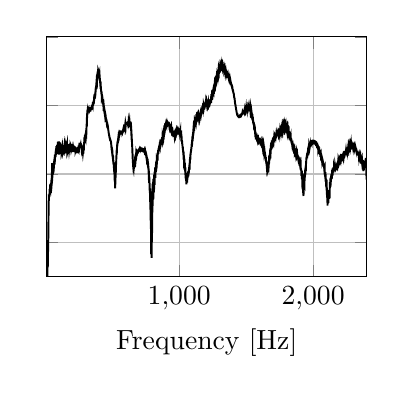
\begin{tikzpicture}

\begin{axis}[%
width=1.6in,
height=1.2in,
at={(1.011in,0.642in)},
scale only axis,
xmin=10,
xmax=2400,
xmajorgrids,
ymin=-10,
ymax=60,
ymajorgrids,
yticklabels={\empty},
xlabel={Frequency [Hz]},
axis background/.style={fill=white}
]
\addplot [color=black,solid,line width=0.7pt,forget plot]
  table[row sep=crcr]{%
0	-32.9542642844185\\
0.666675926054529	-14.6845655434111\\
1.33335185210906	-19.0012987281109\\
2.00002777816359	-13.9500391696767\\
2.66670370421811	-12.8612059714133\\
3.33337963027264	-1.67740879323293\\
4.00005555632717	-0.624843933806727\\
4.6667314823817	-2.58913325179623\\
5.33340740843623	-11.1605324558409\\
6.00008333449076	-11.469899664391\\
6.66675926054529	-18.5432339910145\\
7.33343518659981	-11.0223388901538\\
8.00011111265434	-7.82993289799328\\
8.66678703870887	-9.60142436024394\\
9.3334629647634	-8.65288592800418\\
10.0001388908179	-13.991879940905\\
10.6668148168725	-6.35863260483617\\
11.333490742927	-8.83967878597772\\
12.0001666689815	-8.49640920122171\\
12.666842595036	-6.34563453163295\\
13.3335185210906	-4.84150131368899\\
14.0001944471451	-2.86115477144844\\
14.6668703731996	-2.3370803092671\\
15.3335462992542	-8.53855825612616\\
16.0002222253087	-10.1640712233529\\
16.6668981513632	-3.91699539045847\\
17.3335740774177	-1.81357849731365\\
18.0002500034723	-3.69642389414687\\
18.6669259295268	-6.86272637365297\\
19.3336018555813	-6.75672037001779\\
20.0002777816359	-3.22279072418833\\
20.6669537076904	-0.245849704897205\\
21.3336296337449	0.555046328428655\\
22.0003055597994	1.20865167629159\\
22.666981485854	2.15022410883011\\
23.3336574119085	5.82953589514381\\
24.000333337963	8.40437010009167\\
24.6670092640176	10.3339687022174\\
25.3336851900721	12.4473388468142\\
26.0003611161266	12.370134956199\\
26.6670370421811	12.8976853418347\\
27.3337129682357	13.2731300466608\\
28.0003888942902	13.7031407847312\\
28.6670648203447	13.8013739157546\\
29.3337407463993	13.4196453570526\\
30.0004166724538	13.4729559849866\\
30.6670925985083	14.0461018624098\\
31.3337685245628	14.9346960479171\\
32.0004444506174	15.3361757688169\\
32.6671203766719	15.6313667287765\\
33.3337963027264	15.010432664101\\
34.000472228781	14.6093108973988\\
34.6671481548355	15.3627133304535\\
35.33382408089	16.5119438075708\\
36.0005000069445	16.9971886115222\\
36.6671759329991	16.469694306863\\
37.3338518590536	15.6277155266518\\
38.0005277851081	15.5246110560529\\
38.6672037111627	16.2755470351885\\
39.3338796372172	16.4525530893643\\
40.0005555632717	15.2303821994729\\
40.6672314893262	14.487043407189\\
41.3339074153808	16.2083065645607\\
42.0005833414353	17.422669575197\\
42.6672592674898	16.4592554188264\\
43.3339351935444	15.1034907354332\\
44.0006111195989	17.0111241782868\\
44.6672870456534	18.201490965331\\
45.3339629717079	16.8667279202348\\
46.0006388977625	15.7159850113633\\
46.667314823817	18.0001431368345\\
47.3339907498715	18.7255963891366\\
48.0006666759261	17.1594510141795\\
48.6673426019806	17.5901560818926\\
49.3340185280351	19.374460971314\\
50.0006944540896	23.1601972834232\\
50.6673703801442	17.9574241973792\\
51.3340463061987	19.4873316027077\\
52.0007222322532	20.0341077786872\\
52.6673981583078	18.9503463338701\\
53.3340740843623	19.5176150605708\\
54.0007500104168	20.721367368529\\
54.6674259364713	20.1342110747392\\
55.3341018625259	19.7794570285275\\
56.0007777885804	21.1345939181748\\
56.6674537146349	21.047444991182\\
57.3341296406895	20.0019670417853\\
58.000805566744	21.487331397091\\
58.6674814927985	21.9300203016058\\
59.334157418853	20.4192571441477\\
60.0008333449076	21.967943906294\\
60.6675092709621	22.4891123503144\\
61.3341851970166	20.7882188843823\\
62.0008611230712	22.8026326611608\\
62.6675370491257	22.874358718994\\
63.3342129751802	21.6437756372414\\
64.0008889012347	23.3854363766508\\
64.6675648272893	22.7106002565169\\
65.3342407533438	22.9327427304301\\
66.0009166793983	23.8440260773282\\
66.6675926054529	22.6553110655158\\
67.3342685315074	23.8864548526909\\
68.0009444575619	24.3364081956324\\
68.6676203836164	22.8209283911257\\
69.334296309671	24.8377196410644\\
70.0009722357255	24.4571853620824\\
70.66764816178	23.5870307673301\\
71.3343240878346	25.6650302442439\\
72.0010000138891	23.7517238350044\\
72.6676759399436	25.5175196030082\\
73.3343518659981	24.7699427075374\\
74.0010277920527	25.3723742217785\\
74.6677037181072	25.5532295394115\\
75.3343796441617	24.9029507205431\\
76.0010555702163	26.5461641588184\\
76.6677314962708	25.0930559906814\\
77.3344074223253	26.2233799142036\\
78.0010833483798	26.6337418170719\\
78.6677592744344	25.5743696855721\\
79.3344352004889	27.0921903963245\\
80.0011111265434	25.9119907263925\\
80.667787052598	27.5134016819859\\
81.3344629786525	25.8781343459226\\
82.001138904707	28.111836589389\\
82.6678148307615	26.1069174766483\\
83.3344907568161	28.1061319723714\\
84.0011666828706	27.0941779128178\\
84.6678426089251	27.8644476077528\\
85.3345185349797	27.5678216920856\\
86.0011944610342	28.1485980308591\\
86.6678703870887	27.635515447402\\
87.3345463131432	28.4615092755513\\
88.0012222391978	27.7879428090631\\
88.6678981652523	28.460618789604\\
89.3345740913068	27.9538767366154\\
90.0012500173614	28.4415830747073\\
90.6679259434159	27.6840832714515\\
91.3346018694704	28.6035160163689\\
92.0012777955249	27.3531700036025\\
92.6679537215795	28.8419095326199\\
93.334629647634	26.7725818377304\\
94.0013055736885	29.3929659358635\\
94.667981499743	25.7725908845774\\
95.3346574257976	29.4809770140078\\
96.0013333518521	26.331945213629\\
96.6680092779066	28.6944834367365\\
97.3346852039612	27.2743492116346\\
98.0013611300157	28.4648587575724\\
98.6680370560702	27.3790621914778\\
99.3347129821248	27.8319961551019\\
100.001388908179	28.5950235149963\\
100.668064834234	25.6308542451117\\
101.334740760288	29.5532531851656\\
102.001416686343	26.3472668522608\\
102.668092612397	28.335683088492\\
103.334768538452	28.3520391292351\\
104.001444464506	26.683343568046\\
104.668120390561	28.4445359914923\\
105.334796316616	26.6796454585662\\
106.00147224267	28.6752164667373\\
106.668148168725	27.5593725364504\\
107.334824094779	26.306657550631\\
108.001500020834	29.264379128242\\
108.668175946888	26.9267442548391\\
109.334851872943	27.2017840376286\\
110.001527798997	28.0110388169892\\
110.668203725052	26.3288639454228\\
111.334879651106	28.8178007412704\\
112.001555577161	27.0090561842717\\
112.668231503215	26.6292046028306\\
113.33490742927	28.3264678302833\\
114.001583355324	27.4009484627017\\
114.668259281379	26.4333513977906\\
115.334935207433	27.6077816096871\\
116.001611133488	26.9450505136764\\
116.668287059542	28.167555285332\\
117.334962985597	27.5666658556031\\
118.001638911652	25.8212906750508\\
118.668314837706	26.8154868668093\\
119.334990763761	28.3629572760019\\
120.001666689815	27.5899688366919\\
120.66834261587	27.2977783165281\\
121.335018541924	26.0987768347349\\
122.001694467979	26.1949232368855\\
122.668370394033	27.3352466213392\\
123.335046320088	28.4862125487164\\
124.001722246142	27.7683430226388\\
124.668398172197	27.9156037341288\\
125.335074098251	27.2446360417053\\
126.001750024306	26.9078961527668\\
126.66842595036	26.6268085377659\\
127.335101876415	27.6788095680259\\
128.001777802469	27.3666563536941\\
128.668453728524	27.23736917241\\
129.335129654579	27.2219241998279\\
130.001805580633	26.7946220604895\\
130.668481506688	26.2299138306069\\
131.335157432742	26.3263179304689\\
132.001833358797	27.7113085622301\\
132.668509284851	27.8254150880695\\
133.335185210906	28.2082872947396\\
134.00186113696	28.2031050556989\\
134.668537063015	28.4339046305756\\
135.335212989069	27.8996378529423\\
136.001888915124	27.0126099094661\\
136.668564841178	27.1013103213132\\
137.335240767233	26.9902523116447\\
138.001916693287	27.2157217633037\\
138.668592619342	26.6582802881658\\
139.335268545396	27.0322330388277\\
140.001944471451	27.5703660268133\\
140.668620397506	27.6790044435994\\
141.33529632356	27.8647791859601\\
142.001972249615	27.6435046079511\\
142.668648175669	28.2664479957881\\
143.335324101724	28.5063871061597\\
144.002000027778	28.2817362320478\\
144.668675953833	28.1766961818202\\
145.335351879887	27.6526232083338\\
146.002027805942	27.9122021074423\\
146.668703731996	28.1178740431468\\
147.335379658051	27.8334145498168\\
148.002055584105	27.8224613524614\\
148.66873151016	27.3423083974922\\
149.335407436214	27.4591975741372\\
150.002083362269	28.2291173981817\\
150.668759288323	28.2815859605817\\
151.335435214378	28.5898454164182\\
152.002111140433	28.475248077444\\
152.668787066487	27.8309666724091\\
153.335462992542	27.8259300448496\\
154.002138918596	27.6505532102419\\
154.668814844651	27.3902705700916\\
155.335490770705	27.4185219538949\\
156.00216669676	26.6858474254093\\
156.668842622814	26.0320586251258\\
157.335518548869	26.5128083722324\\
158.002194474923	26.9747812935418\\
158.668870400978	27.300096628394\\
159.335546327032	27.7876872521218\\
160.002222253087	27.6769038007436\\
160.668898179141	27.8079681014809\\
161.335574105196	28.6588334375378\\
162.00225003125	28.7911937360878\\
162.668925957305	27.8754852137226\\
163.335601883359	26.8420303249121\\
164.002277809414	26.1368004249838\\
164.668953735469	26.2320102920629\\
165.335629661523	27.0588230380753\\
166.002305587578	27.6251465726621\\
166.668981513632	27.5486110945447\\
167.335657439687	27.7249852750679\\
168.002333365741	28.2807472448309\\
168.669009291796	28.2299268652934\\
169.33568521785	27.4074713797279\\
170.002361143905	27.0723622756352\\
170.669037069959	27.7986891322903\\
171.335712996014	28.4149057683991\\
172.002388922068	28.4268629825006\\
172.669064848123	27.8959897572276\\
173.335740774177	26.7907781438836\\
174.002416700232	26.8429234491551\\
174.669092626286	27.9419455872997\\
175.335768552341	27.9895940170036\\
176.002444478396	27.0686357078794\\
176.66912040445	27.0290680199997\\
177.335796330505	27.2954833413805\\
178.002472256559	26.9536279615557\\
178.669148182614	27.1540979559818\\
179.335824108668	27.8784616099575\\
180.002500034723	27.2264739205741\\
180.669175960777	26.4007589161582\\
181.335851886832	27.6958385477856\\
182.002527812886	27.8595893726869\\
182.669203738941	27.0565093190054\\
183.335879664995	27.2810846133565\\
184.00255559105	27.8992504238022\\
184.669231517104	27.9801371252967\\
185.335907443159	27.7170268688525\\
186.002583369213	28.0430554404551\\
186.669259295268	27.9997399825154\\
187.335935221323	28.5914688204431\\
188.002611147377	28.5194171359001\\
188.669287073432	27.8081051209744\\
189.335962999486	28.6796629297339\\
190.002638925541	28.0326022599609\\
190.669314851595	27.6421611101028\\
191.33599077765	28.1480673086878\\
192.002666703704	26.933659057478\\
192.669342629759	27.2999158219966\\
193.336018555813	27.0502770289362\\
194.002694481868	27.16139114113\\
194.669370407922	28.2654681423943\\
195.336046333977	27.3004571648008\\
196.002722260031	28.6472460961702\\
196.669398186086	28.1519378604909\\
197.33607411214	28.346411895017\\
198.002750038195	28.3406982483086\\
198.66942596425	27.5527737530556\\
199.336101890304	27.2444348894403\\
200.002777816359	27.126722200162\\
200.669453742413	27.1039130044444\\
201.336129668468	27.9451858741092\\
202.002805594522	28.0526491794506\\
202.669481520577	28.8195105464835\\
203.336157446631	27.7548019531561\\
204.002833372686	27.9457589378811\\
204.66950929874	26.4218916067479\\
205.336185224795	27.4782335537777\\
206.002861150849	27.1323881569617\\
206.669537076904	28.5896343664195\\
207.336213002958	28.0023006574101\\
208.002888929013	28.3706147619349\\
208.669564855067	26.9827836753058\\
209.336240781122	27.3107156431236\\
210.002916707176	27.1469055056564\\
210.669592633231	27.8861389464631\\
211.336268559286	27.8105990214694\\
212.00294448534	27.7128953957855\\
212.669620411395	27.2338771046738\\
213.336296337449	27.4245070874066\\
214.002972263504	28.2274322086808\\
214.669648189558	27.928453394102\\
215.336324115613	27.8367017419009\\
216.003000041667	26.5063574289314\\
216.669675967722	27.0667348767854\\
217.336351893776	27.0998670234007\\
218.003027819831	27.8540239867062\\
218.669703745885	27.1363845776686\\
219.33637967194	26.8249836875644\\
220.003055597994	27.9289355794102\\
220.669731524049	27.7039854123365\\
221.336407450103	28.0790998393347\\
222.003083376158	27.3519434962646\\
222.669759302213	27.0239264431326\\
223.336435228267	27.982809986859\\
224.003111154322	27.2908331736022\\
224.669787080376	26.6119869992078\\
225.336463006431	26.6947470084659\\
226.003138932485	27.1164412767193\\
226.66981485854	26.867154977483\\
227.336490784594	26.0468486154129\\
228.003166710649	26.5698662932687\\
228.669842636703	27.4316612748119\\
229.336518562758	26.1774468466449\\
230.003194488812	26.4048460290718\\
230.669870414867	27.5214832924402\\
231.336546340921	26.804152502656\\
232.003222266976	26.4409215098425\\
232.66989819303	27.3563869176491\\
233.336574119085	27.3760299226242\\
234.00325004514	26.2957045668907\\
234.669925971194	27.0413509709226\\
235.336601897249	27.5625093349253\\
236.003277823303	26.6067414830425\\
236.669953749358	26.6001690068565\\
237.336629675412	27.3486100946739\\
238.003305601467	26.8386796182039\\
238.669981527521	26.5921179722243\\
239.336657453576	27.1642223701848\\
240.00333337963	26.5065818791848\\
240.670009305685	26.2183618830366\\
241.336685231739	27.1077252529932\\
242.003361157794	26.805775609893\\
242.670037083848	26.3978794910355\\
243.336713009903	26.4067842887105\\
244.003388935957	26.1623742353433\\
244.670064862012	26.6754305036207\\
245.336740788066	26.8738364634085\\
246.003416714121	26.1787943821231\\
246.670092640176	26.6952077476482\\
247.33676856623	26.6074658079014\\
248.003444492285	26.5622589619372\\
248.670120418339	26.9886488616443\\
249.336796344394	26.5274746664524\\
250.003472270448	27.2603649494661\\
250.670148196503	27.4976579427953\\
251.336824122557	27.4561113286206\\
252.003500048612	27.882197194409\\
252.670175974666	27.5748599793479\\
253.336851900721	28.0936797777742\\
254.003527826775	28.2561165953469\\
254.67020375283	28.670873792753\\
255.336879678884	29.0796155515953\\
256.003555604939	28.8466950170801\\
256.670231530993	29.1021017575581\\
257.336907457048	28.6211392128075\\
258.003583383103	28.6324379397429\\
258.670259309157	28.1911501244665\\
259.336935235212	28.0078095555882\\
260.003611161266	27.9531890996954\\
260.670287087321	27.7008631339077\\
261.336963013375	28.0513590345836\\
262.00363893943	28.1474486540021\\
262.670314865484	28.4933580093952\\
263.336990791539	28.5217082706304\\
264.003666717593	28.6278493072991\\
264.670342643648	28.4275411676112\\
265.337018569702	28.2587739202446\\
266.003694495757	27.9181995413403\\
266.670370421811	27.6204792265157\\
267.337046347866	27.8612996569514\\
268.00372227392	28.0806348053668\\
268.670398199975	28.4130511059115\\
269.33707412603	28.3865529560878\\
270.003750052084	28.3339863402989\\
270.670425978139	27.7083107744588\\
271.337101904193	27.4001340359726\\
272.003777830248	27.0390602499478\\
272.670453756302	27.160228181464\\
273.337129682357	27.4005657908497\\
274.003805608411	27.5854686973033\\
274.670481534466	27.556050360991\\
275.33715746052	26.9853572539847\\
276.003833386575	26.8999919384363\\
276.670509312629	26.6177794038615\\
277.337185238684	27.3132122908358\\
278.003861164738	27.2275636209128\\
278.670537090793	27.5957629959945\\
279.337213016847	26.8935314416699\\
280.003888942902	26.4562187476062\\
280.670564868956	26.1877355727709\\
281.337240795011	26.4186558195919\\
282.003916721066	27.1888432128385\\
282.67059264712	26.7151359865905\\
283.337268573175	26.6157068180719\\
284.003944499229	25.9862492165293\\
284.670620425284	26.4460018049371\\
285.337296351338	27.3017175462574\\
286.003972277393	27.3199670571856\\
286.670648203447	27.479647480739\\
287.337324129502	26.9278317858887\\
288.004000055556	27.6233103937906\\
288.670675981611	28.788291616744\\
289.337351907665	29.0608872359946\\
290.00402783372	29.2847317438504\\
290.670703759774	28.8574448293116\\
291.337379685829	29.3555320941704\\
292.004055611883	30.5443613834289\\
292.670731537938	30.5835150816502\\
293.337407463993	30.5211650671297\\
294.004083390047	30.4816935746342\\
294.670759316102	30.6313328249626\\
295.337435242156	31.2553239469366\\
296.004111168211	30.8343988195158\\
296.670787094265	30.3733976244532\\
297.33746302032	31.2571848513829\\
298.004138946374	31.3492827360965\\
298.670814872429	30.6724875392444\\
299.337490798483	30.750983357054\\
300.004166724538	30.9693698413865\\
300.670842650592	30.8153276114163\\
301.337518576647	30.6652332383761\\
302.004194502701	30.5206903183156\\
302.670870428756	30.861424015706\\
303.33754635481	31.3148619833261\\
304.004222280865	31.121572336842\\
304.67089820692	31.2553188527646\\
305.337574132974	32.1741216300989\\
306.004250059029	32.614070255134\\
306.670925985083	32.4923061110064\\
307.337601911138	33.2666826153498\\
308.004277837192	34.4129753020652\\
308.670953763247	34.4260456547184\\
309.337629689301	34.7050370904796\\
310.004305615356	35.9497739844772\\
310.67098154141	36.3548158805279\\
311.337657467465	36.2197512607547\\
312.004333393519	37.0454393635388\\
312.671009319574	37.5817876693966\\
313.337685245628	37.3730472531356\\
314.004361171683	37.8742823802724\\
314.671037097737	38.118788117127\\
315.337713023792	37.8989108769071\\
316.004388949847	38.4089983126557\\
316.671064875901	38.9614441710121\\
317.337740801956	38.0495520593038\\
318.00441672801	38.2027655223512\\
318.671092654065	39.4354616793623\\
319.337768580119	38.338207641124\\
320.004444506174	38.6153183348196\\
320.671120432228	39.0100651426825\\
321.337796358283	38.2771645658296\\
322.004472284337	39.2395597689691\\
322.671148210392	39.2758343939724\\
323.337824136446	38.2638813860983\\
324.004500062501	38.647285304051\\
324.671175988555	39.0274459397685\\
325.33785191461	38.4459494901853\\
326.004527840664	39.4866483597124\\
326.671203766719	38.6026957924565\\
327.337879692774	38.169448898158\\
328.004555618828	38.8347209505799\\
328.671231544883	38.3917001395404\\
329.337907470937	38.8984831991535\\
330.004583396992	39.2373179432691\\
330.671259323046	38.1958077498958\\
331.337935249101	39.0940812603407\\
332.004611175155	38.4494955366256\\
332.67128710121	38.4933247851354\\
333.337963027264	39.2643731396367\\
334.004638953319	38.2701520164117\\
334.671314879373	39.4312484788465\\
335.337990805428	38.6631786371716\\
336.004666731482	38.4344447190109\\
336.671342657537	39.0006501349325\\
337.338018583591	38.1799409699282\\
338.004694509646	39.3250988872624\\
338.671370435701	38.6356364870404\\
339.338046361755	39.0568397937205\\
340.00472228781	39.3759468441284\\
340.671398213864	38.7417063612969\\
341.338074139919	39.3943132810887\\
342.004750065973	38.6617589596115\\
342.671425992028	39.4831488754882\\
343.338101918082	38.6220224927181\\
344.004777844137	39.118608763302\\
344.671453770191	39.2033936782924\\
345.338129696246	38.7806353510911\\
346.0048056223	39.7474423420957\\
346.671481548355	39.2189884139585\\
347.338157474409	39.877928712794\\
348.004833400464	39.2233345365668\\
348.671509326518	40.1355248044481\\
349.338185252573	39.3174209853609\\
350.004861178627	40.1811671723392\\
350.671537104682	39.8367887177317\\
351.338213030737	39.8095882548078\\
352.004888956791	39.8767005020069\\
352.671564882846	40.0686976450117\\
353.3382408089	40.0096640618108\\
354.004916734955	39.9130012971316\\
354.671592661009	40.3680982078291\\
355.338268587064	39.8819708948193\\
356.004944513118	40.5783880483702\\
356.671620439173	40.0584427105915\\
357.338296365227	40.7342647667874\\
358.004972291282	40.234418247084\\
358.671648217336	40.8217349517772\\
359.338324143391	40.4888184371648\\
360.005000069445	40.9921762235535\\
360.6716759955	40.699193243542\\
361.338351921554	41.363619185061\\
362.005027847609	40.9275771894624\\
362.671703773664	41.4879104374902\\
363.338379699718	41.2530912044148\\
364.005055625773	41.758174519424\\
364.671731551827	41.6815108531865\\
365.338407477882	41.9266505643339\\
366.005083403936	42.2890056807139\\
366.671759329991	41.9439126071246\\
367.338435256045	42.6130501067571\\
368.0051111821	42.1908654276791\\
368.671787108154	43.1464799716712\\
369.338463034209	42.3066660890061\\
370.005138960263	43.4097744757615\\
370.671814886318	42.5771136099711\\
371.338490812372	43.3434998142006\\
372.005166738427	43.0679053511227\\
372.671842664481	43.4388379202172\\
373.338518590536	43.6240614025757\\
374.005194516591	43.5981686533101\\
374.671870442645	44.3385279614038\\
375.3385463687	43.9455741601809\\
376.005222294754	44.8868080737712\\
376.671898220809	44.6465650757257\\
377.338574146863	44.9244910506111\\
378.005250072918	45.3596799106132\\
378.671925998972	44.7965295096707\\
379.338601925027	45.7965611169359\\
380.005277851081	45.2553541440655\\
380.671953777136	46.0180445392896\\
381.33862970319	46.3749031615187\\
382.005305629245	46.1913599854019\\
382.671981555299	47.2322581860385\\
383.338657481354	46.5210403394097\\
384.005333407408	47.3393812127016\\
384.672009333463	47.4335611379163\\
385.338685259517	47.299665107107\\
386.005361185572	48.451928200437\\
386.672037111627	47.9144798628308\\
387.338713037681	48.6096993791366\\
388.005388963736	48.7509529148685\\
388.67206488979	48.2259178138567\\
389.338740815845	49.3033118817462\\
390.005416741899	48.959868892596\\
390.672092667954	49.3039733585486\\
391.338768594008	49.8413385727934\\
392.005444520063	49.2471033573352\\
392.672120446117	49.6684559270224\\
393.338796372172	50.1483759360299\\
394.005472298226	49.7511505211498\\
394.672148224281	50.3526533520252\\
395.338824150335	50.2730733145507\\
396.00550007639	49.6339327314993\\
396.672176002444	50.4674931152044\\
397.338851928499	50.2923160535964\\
398.005527854554	49.7214928886323\\
398.672203780608	50.1593263405583\\
399.338879706663	49.973977802395\\
400.005555632717	49.3226171550465\\
400.672231558772	50.039741483087\\
401.338907484826	49.5809952696733\\
402.005583410881	48.5897735225678\\
402.672259336935	49.2840273117474\\
403.33893526299	49.3882443584783\\
404.005611189044	48.1497229793152\\
404.672287115099	48.1902661093348\\
405.338963041153	48.9595228652248\\
406.005638967208	47.8182559831111\\
406.672314893262	47.2463745161268\\
407.338990819317	47.8557554543192\\
408.005666745371	47.7969490714689\\
408.672342671426	46.512518231193\\
409.339018597481	46.6734252859241\\
410.005694523535	47.2115173206619\\
410.67237044959	46.1661385803392\\
411.339046375644	45.5703689989209\\
412.005722301699	46.1526510802663\\
412.672398227753	46.1847367123389\\
413.339074153808	44.9553068046714\\
414.005750079862	44.7014204211387\\
414.672426005917	45.5445450676173\\
415.339101931971	44.9792722834595\\
416.005777858026	44.0700145202577\\
416.67245378408	44.342218470384\\
417.339129710135	44.5984321783226\\
418.005805636189	44.0551024588523\\
418.672481562244	43.4030261914705\\
419.339157488298	43.6162105472245\\
420.005833414353	43.9522071893011\\
420.672509340407	43.4819024975137\\
421.339185266462	42.6500995803272\\
422.005861192517	42.7720406092537\\
422.672537118571	43.2815520289521\\
423.339213044626	43.1044621354194\\
424.00588897068	42.3053058273224\\
424.672564896735	41.9553511630938\\
425.339240822789	42.3201801980656\\
426.005916748844	42.5766658558122\\
426.672592674898	41.9484077404209\\
427.339268600953	41.3317803158795\\
428.005944527007	41.593356396085\\
428.672620453062	41.7037355132992\\
429.339296379116	41.6425130905545\\
430.005972305171	41.1329748054101\\
430.672648231225	40.3307476311112\\
431.33932415728	40.580335691839\\
432.006000083334	40.9630686937739\\
432.672676009389	40.9748662554684\\
433.339351935444	40.4072997447932\\
434.006027861498	39.7354349678651\\
434.672703787553	39.8047798096333\\
435.339379713607	39.9228654612959\\
436.006055639662	40.050737774686\\
436.672731565716	39.7589500448515\\
437.339407491771	39.1689590407012\\
438.006083417825	38.7017551603367\\
438.67275934388	38.5803374169027\\
439.339435269934	39.05426245116\\
440.006111195989	39.107184261764\\
440.672787122043	38.9471102722804\\
441.339463048098	38.2374375318609\\
442.006138974152	37.9421683609842\\
442.672814900207	37.7726802909328\\
443.339490826261	38.0331016519881\\
444.006166752316	38.1464192272895\\
444.672842678371	38.1235110966163\\
445.339518604425	37.9134696942787\\
446.00619453048	37.4564242759909\\
446.672870456534	37.008131472359\\
447.339546382589	36.7279854254299\\
448.006222308643	36.8448913005371\\
448.672898234698	37.0570461397611\\
449.339574160752	37.2556794144867\\
450.006250086807	37.1220909262624\\
450.672926012861	36.8041801843687\\
451.339601938916	36.3796768668171\\
452.00627786497	35.9397030952869\\
452.672953791025	35.711911396731\\
453.339629717079	35.6400819721962\\
454.006305643134	35.7966089242675\\
454.672981569188	35.8036435847489\\
455.339657495243	35.926466195374\\
456.006333421298	35.8271545729255\\
456.673009347352	35.7928516689946\\
457.339685273407	35.4751990938894\\
458.006361199461	35.2450651140489\\
458.673037125516	34.9228136005966\\
459.33971305157	34.6427893934498\\
460.006388977625	34.4211309336367\\
460.673064903679	34.2524349742398\\
461.339740829734	34.3079395565215\\
462.006416755788	34.2195203664308\\
462.673092681843	34.3287909769097\\
463.339768607897	34.3479993210939\\
464.006444533952	34.3358280201436\\
464.673120460006	34.3945424529362\\
465.339796386061	34.2685444334078\\
466.006472312115	34.2411682067034\\
466.67314823817	34.0241377712959\\
467.339824164225	33.8548556210211\\
468.006500090279	33.6561384644472\\
468.673176016334	33.314421419094\\
469.339851942388	33.1803434966029\\
470.006527868443	32.8968575543437\\
470.673203794497	32.6741546331654\\
471.339879720552	32.5848669208083\\
472.006555646606	32.317953536263\\
472.673231572661	32.1338108992383\\
473.339907498715	31.997288964322\\
474.00658342477	31.7946706686206\\
474.673259350824	31.7232550755955\\
475.339935276879	31.5956853372537\\
476.006611202933	31.3664299474193\\
476.673287128988	31.2707524412126\\
477.339963055042	31.1419520691542\\
478.006638981097	30.9542750783129\\
478.673314907152	30.9551661515827\\
479.339990833206	30.8022937778166\\
480.006666759261	30.5442514056002\\
480.673342685315	30.4826951810165\\
481.34001861137	30.4282304200776\\
482.006694537424	30.255240329131\\
482.673370463479	30.1141854265219\\
483.340046389533	30.0843506574158\\
484.006722315588	29.9166865547759\\
484.673398241642	29.9006294361052\\
485.340074167697	29.8643402977968\\
486.006750093751	29.7785551892122\\
486.673426019806	29.7228287804329\\
487.34010194586	29.7764869351763\\
488.006777871915	29.6989002850878\\
488.673453797969	29.6076291886936\\
489.340129724024	29.5005914039469\\
490.006805650078	29.4673356311453\\
490.673481576133	29.1778402805032\\
491.340157502188	28.9487810622075\\
492.006833428242	28.6670848987879\\
492.673509354297	28.3954740848811\\
493.340185280351	28.0596408437528\\
494.006861206406	27.6868759830443\\
494.67353713246	27.439519447154\\
495.340213058515	27.2008367353398\\
496.006888984569	27.186451270908\\
496.673564910624	26.9646492839064\\
497.340240836678	27.078237671534\\
498.006916762733	27.1539828160005\\
498.673592688787	27.197993080158\\
499.340268614842	27.0353534017953\\
500.006944540896	26.8544073335033\\
500.673620466951	26.5261369799915\\
501.340296393005	26.0814107628716\\
502.00697231906	25.6388112161935\\
502.673648245115	25.1489975457236\\
503.340324171169	24.9317970565909\\
504.007000097224	25.1264218041706\\
504.673676023278	25.1372985326933\\
505.340351949333	25.3913820064347\\
506.007027875387	25.1197332353229\\
506.673703801442	24.6972041355198\\
507.340379727496	24.1655309495926\\
508.007055653551	23.629244596529\\
508.673731579605	23.1911160932314\\
509.34040750566	23.1705486845897\\
510.007083431714	23.2304831944749\\
510.673759357769	23.2009686181264\\
511.340435283823	23.2021857781483\\
512.007111209878	22.5781174166447\\
512.673787135932	21.5837393020493\\
513.340463061987	20.9274163555549\\
514.007138988041	20.7921048102855\\
514.673814914096	20.9102915105759\\
515.340490840151	20.9277198141672\\
516.007166766205	20.6110812756809\\
516.67384269226	19.326467175344\\
517.340518618314	18.4135742470128\\
518.007194544369	18.3249966311569\\
518.673870470423	17.6860896240802\\
519.340546396478	18.4295796966118\\
520.007222322532	18.4755494436701\\
520.673898248587	18.0407828999954\\
521.340574174641	16.1584635936708\\
522.007250100696	15.8123329055694\\
522.67392602675	17.7510961157763\\
523.340601952805	18.8040336505348\\
524.007277878859	18.6336653254247\\
524.673953804914	19.3777534863439\\
525.340629730968	19.817508189569\\
526.007305657023	20.2688720770992\\
526.673981583078	21.4198183448291\\
527.340657509132	22.4560973030387\\
528.007333435187	22.7286749366465\\
528.674009361241	23.0546596041959\\
529.340685287296	23.6400817627591\\
530.00736121335	24.5363874129843\\
530.674037139405	25.058342354582\\
531.340713065459	25.4730219892363\\
532.007388991514	25.7459995316439\\
532.674064917568	26.4463530201932\\
533.340740843623	27.0726751951862\\
534.007416769677	27.1100836051329\\
534.674092695732	27.0656279305928\\
535.340768621786	27.8810626202772\\
536.007444547841	28.5954082025088\\
536.674120473896	28.2761526421464\\
537.34079639995	28.2614133930373\\
538.007472326005	28.6418810053646\\
538.674148252059	29.1878908145347\\
539.340824178114	29.2217277599933\\
540.007500104168	28.9652085620643\\
540.674176030223	29.628884633614\\
541.340851956277	29.9446199476455\\
542.007527882332	29.6452701159664\\
542.674203808386	29.6448543709979\\
543.340879734441	30.058821766034\\
544.007555660495	30.2773750186323\\
544.67423158655	29.9954647911668\\
545.340907512604	30.3272149869585\\
546.007583438659	30.8982878294574\\
546.674259364713	30.5630187644663\\
547.340935290768	30.5232331908262\\
548.007611216823	31.1245257451275\\
548.674287142877	31.2277232802882\\
549.340963068932	30.8047323384281\\
550.007638994986	31.2079642158692\\
550.674314921041	31.5531333288068\\
551.340990847095	31.0809173887033\\
552.00766677315	31.2091280445273\\
552.674342699204	31.7840545857256\\
553.341018625259	31.4559525512167\\
554.007694551313	31.4790809477384\\
554.674370477368	32.1126857149522\\
555.341046403422	31.6753911460697\\
556.007722329477	31.6671676960224\\
556.674398255531	32.2485842225792\\
557.341074181586	31.9916168689123\\
558.00775010764	31.7874626142612\\
558.674426033695	32.5294283142161\\
559.341101959749	32.0790366796733\\
560.007777885804	32.0641585864643\\
560.674453811858	32.739236376832\\
561.341129737913	32.0744595161349\\
562.007805663968	32.12725012535\\
562.674481590022	32.6641757885342\\
563.341157516077	31.8852802965691\\
564.007833442131	32.2239490841702\\
564.674509368186	32.4191535334196\\
565.34118529424	31.6383237632574\\
566.007861220295	32.4324083320392\\
566.674537146349	32.1163544766968\\
567.341213072404	31.7625601488521\\
568.007888998458	32.4719095744848\\
568.674564924513	31.7062788922767\\
569.341240850567	31.9788726023617\\
570.007916776622	32.3680390636454\\
570.674592702676	31.4942265391228\\
571.341268628731	32.4190267299822\\
572.007944554785	31.8558531317802\\
572.67462048084	31.8328186398236\\
573.341296406895	32.413540087958\\
574.007972332949	31.802080874944\\
574.674648259004	32.3939317160524\\
575.341324185058	31.9809581517125\\
576.008000111113	32.0466898997641\\
576.674676037167	32.5285418232787\\
577.341351963222	31.9086552944127\\
578.008027889276	32.6517782564659\\
578.674703815331	32.138901639856\\
579.341379741385	32.6257354305967\\
580.00805566744	32.7340154407186\\
580.674731593494	32.3382465779984\\
581.341407519549	33.0328738795281\\
582.008083445603	32.2785835169576\\
582.674759371658	33.1996231867572\\
583.341435297712	32.7971354439217\\
584.008111223767	33.022845212821\\
584.674787149822	32.9995028905735\\
585.341463075876	33.4490233540734\\
586.008139001931	33.2442190711299\\
586.674814927985	33.2857070336147\\
587.34149085404	33.5836150786377\\
588.008166780094	33.1900416476554\\
588.674842706149	33.8551165205642\\
589.341518632203	33.3180816945247\\
590.008194558258	34.209730366845\\
590.674870484312	33.478143628565\\
591.341546410367	34.2176458454027\\
592.008222336421	33.5900889748247\\
592.674898262476	34.3085113022201\\
593.34157418853	33.937888110619\\
594.008250114585	34.4338507139832\\
594.674926040639	33.9714342473181\\
595.341601966694	34.4929931970967\\
596.008277892749	34.1967874208755\\
596.674953818803	34.4211740786626\\
597.341629744858	34.2506189527013\\
598.008305670912	34.6943786724197\\
598.674981596967	34.2847844391941\\
599.341657523021	34.6099506417271\\
600.008333449076	34.4503550569254\\
600.67500937513	34.9179265701357\\
601.341685301185	34.3770392169514\\
602.008361227239	34.8643643376724\\
602.675037153294	34.479281062489\\
603.341713079348	34.9458340920394\\
604.008389005403	34.3510903818293\\
604.675064931457	34.875632689797\\
605.341740857512	34.5781625350259\\
606.008416783566	35.0658803862269\\
606.675092709621	34.4798660980141\\
607.341768635676	35.0506702416938\\
608.00844456173	34.6244822453813\\
608.675120487785	34.9458583469029\\
609.341796413839	34.9465852271203\\
610.008472339894	34.7172958317135\\
610.675148265948	35.1383099962863\\
611.341824192003	34.6592279268889\\
612.008500118057	35.1660666435207\\
612.675176044112	34.690568673943\\
613.341851970166	35.1927443600689\\
614.008527896221	35.0019925650177\\
614.675203822275	34.88317403171\\
615.34187974833	35.2524806452077\\
616.008555674384	34.8038651213053\\
616.675231600439	35.2669614051305\\
617.341907526493	34.8081733014084\\
618.008583452548	35.127549728574\\
618.675259378603	35.1305878692793\\
619.341935304657	35.0333255004886\\
620.008611230711	35.407755413836\\
620.675287156766	34.9261661459017\\
621.341963082821	35.2581871435449\\
622.008639008875	35.0748053153741\\
622.67531493493	34.9874396693013\\
623.341990860984	35.2588661414359\\
624.008666787039	34.9302370659396\\
624.675342713093	35.2406294957468\\
625.342018639148	35.2302506205488\\
626.008694565202	34.9534798776054\\
626.675370491257	35.2827410807569\\
627.342046417311	35.0082170931189\\
628.008722343366	35.1016648147968\\
628.67539826942	35.2867472863993\\
629.342074195475	34.9277443704084\\
630.008750121529	35.226685146609\\
630.675426047584	35.1504975010966\\
631.342101973638	34.7696720003473\\
632.008777899693	35.2699564502557\\
632.675453825748	34.8694598684105\\
633.342129751802	34.7123652482083\\
634.008805677857	35.0530807217269\\
634.675481603911	34.5991549198923\\
635.342157529966	34.5015677080545\\
636.00883345602	34.7877217754514\\
636.675509382075	34.2637760430924\\
637.342185308129	34.1156398236885\\
638.008861234184	34.4000081945685\\
638.675537160238	33.7913220389294\\
639.342213086293	33.4761841935138\\
640.008889012347	33.7624306935067\\
640.675564938402	33.1692121517248\\
641.342240864456	32.6768725549582\\
642.008916790511	32.8445740558807\\
642.675592716565	32.4164637429366\\
643.34226864262	31.6342690276707\\
644.008944568675	31.6330377495722\\
644.675620494729	31.3532381257952\\
645.342296420784	30.5377253923522\\
646.008972346838	29.9522133617675\\
646.675648272893	29.8868907479859\\
647.342324198947	28.9555890854284\\
648.009000125002	28.3172772947539\\
648.675676051056	28.1801783749749\\
649.342351977111	27.4941353537044\\
650.009027903165	26.5626546782851\\
650.67570382922	26.1277350380964\\
651.342379755274	25.8332038382809\\
652.009055681329	25.1616811331085\\
652.675731607383	24.3994895991991\\
653.342407533438	23.9749387784302\\
654.009083459492	23.8839640864832\\
654.675759385547	22.9822809244442\\
655.342435311602	22.3751035633959\\
656.009111237656	22.2627726887099\\
656.675787163711	21.9898526944988\\
657.342463089765	22.1103858462562\\
658.00913901582	21.8900258724702\\
658.675814941874	21.5122337348614\\
659.342490867929	21.3678123253984\\
660.009166793983	21.7132005085055\\
660.675842720038	21.9091883369201\\
661.342518646092	21.7565784026932\\
662.009194572147	21.9715984896753\\
662.675870498201	22.2083472843096\\
663.342546424256	22.3288076307321\\
664.00922235031	22.4026360893313\\
664.675898276365	22.5185216428069\\
665.342574202419	22.5225939011441\\
666.009250128474	23.0094550171569\\
666.675926054529	23.4121199769689\\
667.342601980583	23.6040842561816\\
668.009277906638	23.4017476023075\\
668.675953832692	23.3224404941483\\
669.342629758747	23.8183878120188\\
670.009305684801	24.2129595524648\\
670.675981610856	24.1648519136487\\
671.34265753691	24.116125383029\\
672.009333462965	24.1918540783631\\
672.676009389019	24.3539002982706\\
673.342685315074	24.7784421020204\\
674.009361241128	24.8689648290229\\
674.676037167183	24.9954563486901\\
675.342713093237	24.9385661117814\\
676.009389019292	24.7278268476489\\
676.676064945346	25.0047166338498\\
677.342740871401	25.2985844404401\\
678.009416797456	25.7240278397373\\
678.67609272351	25.5636002320469\\
679.342768649565	25.3533788797872\\
680.009444575619	25.2729622835602\\
680.676120501674	25.4929029526025\\
681.342796427728	25.7648934715001\\
682.009472353783	25.9572330888222\\
682.676148279837	26.1121267412993\\
683.342824205892	26.0097942828218\\
684.009500131946	25.8734731797464\\
684.676176058001	25.8519695467487\\
685.342851984055	25.9930109633483\\
686.00952791011	26.0630311157454\\
686.676203836164	26.3183293949466\\
687.342879762219	26.5218048482159\\
688.009555688273	26.5342305919842\\
688.676231614328	26.5082676555348\\
689.342907540382	26.3548406604347\\
690.009583466437	26.1958804762066\\
690.676259392492	26.2517090538901\\
691.342935318546	26.3879597700881\\
692.009611244601	26.6432405121635\\
692.676287170655	26.8550879323489\\
693.34296309671	26.9703837530375\\
694.009639022764	26.9965066022829\\
694.676314948819	26.9363735322201\\
695.342990874873	26.7634554177321\\
696.009666800928	26.6998995807277\\
696.676342726982	26.6067386750544\\
697.343018653037	26.653904246167\\
698.009694579091	26.7099790428286\\
698.676370505146	26.8906175206804\\
699.3430464312	26.9765479114423\\
700.009722357255	27.1688996764766\\
700.676398283309	27.2075704714052\\
701.343074209364	27.2981298126844\\
702.009750135419	27.358636852496\\
702.676426061473	27.4075566224886\\
703.343101987528	27.2424593364701\\
704.009777913582	27.2530997175377\\
704.676453839637	27.1865331181\\
705.343129765691	27.1549582668639\\
706.009805691746	27.1032179807976\\
706.6764816178	27.0759194198924\\
707.343157543855	27.0920680840423\\
708.009833469909	27.0873427496582\\
708.676509395964	27.0194248580791\\
709.343185322018	27.1313575762947\\
710.009861248073	27.1807247866304\\
710.676537174127	27.1504225055856\\
711.343213100182	27.1938365148308\\
712.009889026236	27.1796684552453\\
712.676564952291	27.2684206010409\\
713.343240878346	27.2355279304064\\
714.0099168044	27.3192411364001\\
714.676592730455	27.2652129650562\\
715.343268656509	27.3683323450311\\
716.009944582564	27.3825710896875\\
716.676620508618	27.294417858607\\
717.343296434673	27.2957453930704\\
718.009972360727	27.2926898202607\\
718.676648286782	27.2993635296527\\
719.343324212836	27.3107453477551\\
720.010000138891	27.179159518586\\
720.676676064945	27.2136481274604\\
721.343351991	27.2226404257429\\
722.010027917054	27.0749817684709\\
722.676703843109	27.0997483243001\\
723.343379769163	27.0943665126115\\
724.010055695218	27.0243357825009\\
724.676731621273	26.9672424764231\\
725.343407547327	26.9648489687804\\
726.010083473382	26.8584501821819\\
726.676759399436	26.8914059386521\\
727.343435325491	26.9759518599084\\
728.010111251545	27.1122957880035\\
728.6767871776	27.0909276662212\\
729.343463103654	27.1234768819693\\
730.010139029709	27.0912700406679\\
730.676814955763	27.2057522054766\\
731.343490881818	27.1831241403662\\
732.010166807872	27.1950854788672\\
732.676842733927	27.1190816662063\\
733.343518659981	27.0859442747254\\
734.010194586036	26.9949493469146\\
734.67687051209	26.9267070574795\\
735.343546438145	26.7302937566005\\
736.0102223642	26.6279727172532\\
736.676898290254	26.5952355446547\\
737.343574216309	26.4534943287447\\
738.010250142363	26.4303824241115\\
738.676926068418	26.5024239893914\\
739.343601994472	26.5603802102952\\
740.010277920527	26.6719156029096\\
740.676953846581	26.7807961400953\\
741.343629772636	26.6279265723623\\
742.01030569869	26.4635225299507\\
742.676981624745	26.3233656912793\\
743.343657550799	26.1057644017875\\
744.010333476854	26.1314815890242\\
744.677009402908	26.1095040307328\\
745.343685328963	26.0441881771437\\
746.010361255017	26.2499635318896\\
746.677037181072	26.3800993416244\\
747.343713107127	26.1766979662622\\
748.010389033181	26.0465147251119\\
748.677064959236	25.8034265042701\\
749.34374088529	25.6968211906336\\
750.010416811345	25.65779511856\\
750.677092737399	25.6762419705623\\
751.343768663454	25.6506829404138\\
752.010444589508	25.6541876575375\\
752.677120515563	25.6336503560818\\
753.343796441617	25.5651251845963\\
754.010472367672	25.0233244624016\\
754.677148293726	24.8673021671508\\
755.343824219781	25.084555363663\\
756.010500145835	25.2686800355282\\
756.67717607189	25.1501614442518\\
757.343851997944	24.8991278062033\\
758.010527923999	24.6872499913886\\
758.677203850054	24.2743608393458\\
759.343879776108	24.3616319243159\\
760.010555702162	24.596509193122\\
760.677231628217	24.5208686093224\\
761.343907554272	24.0162322541699\\
762.010583480326	23.5655561762011\\
762.677259406381	23.3727728341473\\
763.343935332435	23.4062063983753\\
764.01061125849	24.0089906087017\\
764.677287184544	23.7722701002035\\
765.343963110599	22.9004367389388\\
766.010639036653	22.2366961884461\\
766.677314962708	22.8517962160405\\
767.343990888762	23.1542828326474\\
768.010666814817	22.5897299762969\\
768.677342740871	21.3406742107766\\
769.344018666926	21.6360792404778\\
770.01069459298	21.8607510332222\\
770.677370519035	21.6103375137472\\
771.344046445089	20.8735881819765\\
772.010722371144	20.2148295631305\\
772.677398297199	20.3499468068552\\
773.344074223253	20.9466336690518\\
774.010750149308	19.536773300369\\
774.677426075362	17.3881599480301\\
775.344102001417	18.889687135476\\
776.010777927471	19.4834183372195\\
776.677453853526	18.5270428968694\\
777.34412977958	17.3865396078409\\
778.010805705635	17.5821145276491\\
778.677481631689	16.8758876091287\\
779.344157557744	15.6022247576191\\
780.010833483798	14.6213644689723\\
780.677509409853	14.4582439728314\\
781.344185335907	15.828777802242\\
782.010861261962	13.5199924150568\\
782.677537188016	11.8513026353665\\
783.344213114071	13.9239896001799\\
784.010889040126	13.3226177924555\\
784.67756496618	9.73620384555713\\
785.344240892235	9.6785284159369\\
786.010916818289	10.7264941493107\\
786.677592744344	9.12683077896556\\
787.344268670398	4.73745795103937\\
788.010944596453	10.885038786638\\
788.677620522507	8.78671810400476\\
789.344296448562	-3.32988305528504\\
790.010972374616	9.90022371993913\\
790.677648300671	9.35942203144332\\
791.344324226725	-2.63613688956709\\
792.01100015278	10.2945985141265\\
792.677676078834	10.0658862241892\\
793.344352004889	-4.47966841619267\\
794.011027930943	12.0800712830208\\
794.677703856998	11.9661027067749\\
795.344379783053	0.148097572119663\\
796.011055709107	12.8424686188861\\
796.677731635162	13.0848659009177\\
797.344407561216	2.84541533442673\\
798.011083487271	14.9242723678654\\
798.677759413325	13.8517326859851\\
799.34443533938	8.83718567543206\\
800.011111265434	15.7766153421729\\
800.677787191489	13.2611162040222\\
801.344463117543	10.7427144848108\\
802.011139043598	17.1756493539561\\
802.677814969652	13.1353794852119\\
803.344490895707	14.5104372685328\\
804.011166821761	17.6772787764099\\
804.677842747816	12.5647317524358\\
805.34451867387	16.7606339606418\\
806.011194599925	17.6018603380253\\
806.67787052598	12.8035906238144\\
807.344546452034	18.4843201496526\\
808.011222378089	16.1722129610711\\
808.677898304143	15.6510160998115\\
809.344574230198	18.6894491370345\\
810.011250156252	14.6218195272217\\
810.677926082307	18.1006367189238\\
811.344602008361	18.1777674816091\\
812.011277934416	15.4919094723226\\
812.67795386047	19.8318241252083\\
813.344629786525	16.0565247687491\\
814.011305712579	19.5022065930492\\
814.677981638634	19.3265020591184\\
815.344657564688	17.5280086143724\\
816.011333490743	20.7313819148644\\
816.678009416797	16.8456659583572\\
817.344685342852	20.6486713384342\\
818.011361268907	19.1451905180931\\
818.678037194961	20.0586226271125\\
819.344713121016	21.2183763652885\\
820.01138904707	18.9705840424386\\
820.678064973125	21.9356702557229\\
821.344740899179	18.9154413362866\\
822.011416825234	21.9607054216725\\
822.678092751288	20.309842730348\\
823.344768677343	21.3841366823852\\
824.011444603397	21.6951788204497\\
824.678120529452	20.840582446008\\
825.344796455506	22.7868536253683\\
826.011472381561	20.5659557959512\\
826.678148307615	23.2811308182471\\
827.34482423367	20.9563636602391\\
828.011500159724	23.4766094028297\\
828.678176085779	21.5629613261429\\
829.344852011833	23.8173035309205\\
830.011527937888	21.9712888055879\\
830.678203863943	23.9062849644708\\
831.344879789997	22.919725306612\\
832.011555716052	23.7983409786051\\
832.678231642106	23.6659899533006\\
833.344907568161	24.1321380978359\\
834.011583494215	24.2178105569235\\
834.67825942027	24.0801647374656\\
835.344935346324	24.4419385044434\\
836.011611272379	24.6256166545501\\
836.678287198433	25.0155389292268\\
837.344963124488	24.8192689484527\\
838.011639050542	25.3764273063687\\
838.678314976597	25.3819177769064\\
839.344990902651	25.3154444626054\\
840.011666828706	26.0657894085912\\
840.67834275476	25.7399533534855\\
841.345018680815	26.282299587993\\
842.01169460687	25.8736422748787\\
842.678370532924	26.9414523350636\\
843.345046458979	25.7963383394802\\
844.011722385033	27.1196205985818\\
844.678398311088	25.9189425669728\\
845.345074237142	27.6367129621756\\
846.011750163197	26.4680227771486\\
846.678426089251	27.6103776611331\\
847.345102015306	26.9067423011365\\
848.01177794136	27.6818950155213\\
848.678453867415	27.2101051459883\\
849.345129793469	27.4817743377867\\
850.011805719524	28.2821444398351\\
850.678481645578	27.4586766145298\\
851.345157571633	28.0061835352707\\
852.011833497687	27.1640293145818\\
852.678509423742	28.8235193712824\\
853.345185349797	28.0282244437451\\
854.011861275851	28.3350454743295\\
854.678537201906	28.2861159541651\\
855.34521312796	28.1756974038869\\
856.011889054015	29.2340170024019\\
856.678564980069	28.0614557176998\\
857.345240906124	28.7450611113701\\
858.011916832178	28.6780796060947\\
858.678592758233	28.8383340192278\\
859.345268684287	29.5171602035213\\
860.011944610342	28.2304510889383\\
860.678620536396	28.791020777077\\
861.345296462451	28.7169910595237\\
862.011972388505	28.8915136320869\\
862.67864831456	29.7791924360994\\
863.345324240614	28.7702748709277\\
864.012000166669	29.4619466505887\\
864.678676092724	29.0247575991229\\
865.345352018778	29.0877753533682\\
866.012027944833	30.0846388517136\\
866.678703870887	29.406333546667\\
867.345379796942	29.7493829933118\\
868.012055722996	29.8132823666776\\
868.678731649051	29.2745378248284\\
869.345407575105	29.7622207776571\\
870.01208350116	29.9758234018235\\
870.678759427214	29.97375991458\\
871.345435353269	30.7217255246653\\
872.012111279323	30.2034179044525\\
872.678787205378	30.0183246499807\\
873.345463131432	30.3163375695744\\
874.012139057487	29.745829839652\\
874.678814983541	30.1241402517678\\
875.345490909596	30.8023400971114\\
876.012166835651	30.6504704598168\\
876.678842761705	30.9987688380761\\
877.34551868776	31.5140678839746\\
878.012194613814	31.0249829923555\\
878.678870539869	30.932782335334\\
879.345546465923	31.3090484300808\\
880.012222391978	30.9226057051452\\
880.678898318032	30.791839262032\\
881.345574244087	31.4308558509282\\
882.012250170141	31.4230136280904\\
882.678926096196	31.3807373123212\\
883.34560202225	32.0980346302589\\
884.012277948305	32.2950982623203\\
884.678953874359	32.1321305384195\\
885.345629800414	32.5038607561992\\
886.012305726468	32.824149649699\\
886.678981652523	32.4984488724534\\
887.345657578578	32.5587070139245\\
888.012333504632	33.0721270828866\\
888.679009430687	33.0929046981796\\
889.345685356741	32.8519777230844\\
890.012361282796	33.1303622793269\\
890.67903720885	33.3430769078647\\
891.345713134905	33.2246472566144\\
892.012389060959	33.1501982344552\\
892.679064987014	33.5816347975775\\
893.345740913068	33.6474455778485\\
894.012416839123	33.4402338054538\\
894.679092765177	33.5597782030249\\
895.345768691232	33.7980314509903\\
896.012444617286	33.882190460738\\
896.679120543341	33.5940998569718\\
897.345796469395	33.7521490050265\\
898.01247239545	34.1753658537241\\
898.679148321504	34.3110336173104\\
899.345824247559	34.0857825764243\\
900.012500173613	34.0579784285918\\
900.679176099668	34.3841851068259\\
901.345852025723	34.4926952911963\\
902.012527951777	34.3196477618581\\
902.679203877832	34.2826351777651\\
903.345879803886	34.4946750271042\\
904.012555729941	34.8217885904908\\
904.679231655995	34.789737654975\\
905.34590758205	34.6667018135685\\
906.012583508104	34.5330393669205\\
906.679259434159	34.8188030285893\\
907.345935360213	34.9504548376123\\
908.012611286268	34.7937523660935\\
908.679287212322	34.8146738735634\\
909.345963138377	35.0152658338498\\
910.012639064431	35.0812682296376\\
910.679314990486	35.2556877387032\\
911.34599091654	35.2009921806193\\
912.012666842595	34.9195118053819\\
912.67934276865	34.8102094219661\\
913.346018694704	34.8311936406572\\
914.012694620759	35.031807990024\\
914.679370546813	35.0270457243145\\
915.346046472868	34.9149786238173\\
916.012722398922	34.9348436371736\\
916.679398324977	34.8932719979513\\
917.346074251031	34.9415535469748\\
918.012750177086	34.9921853758109\\
918.67942610314	34.9943446098449\\
919.346102029195	34.5433975725843\\
920.012777955249	34.5802977044847\\
920.679453881304	34.5295196662708\\
921.346129807358	34.6353349296111\\
922.012805733413	34.6307930422955\\
922.679481659467	34.6185425616516\\
923.346157585522	34.6354251229574\\
924.012833511577	34.4403433830772\\
924.679509437631	34.1937640409491\\
925.346185363686	34.0494009534725\\
926.01286128974	34.299092258541\\
926.679537215795	34.3096705676571\\
927.346213141849	33.8523988233306\\
928.012889067904	33.8918900572331\\
928.679564993958	33.8214654139854\\
929.346240920013	33.9003281864181\\
930.012916846067	33.8833280012302\\
930.679592772122	33.4637947666699\\
931.346268698176	33.154061566054\\
932.012944624231	33.4040870037462\\
932.679620550285	33.6917731577573\\
933.34629647634	33.6406154424366\\
934.012972402394	33.5613418931017\\
934.679648328449	33.6088019892989\\
935.346324254504	33.6764833143324\\
936.013000180558	33.2670528690412\\
936.679676106613	33.3412017794513\\
937.346352032667	33.0317352497297\\
938.013027958722	33.3182994880051\\
938.679703884776	33.4506274532857\\
939.346379810831	33.1345382961165\\
940.013055736885	32.9850791623894\\
940.67973166294	33.23102822641\\
941.346407588994	33.1439167198852\\
942.013083515049	33.2899700379283\\
942.679759441103	33.0352325316495\\
943.346435367158	33.7029908661171\\
944.013111293212	33.3271587419532\\
944.679787219267	33.203935031084\\
945.346463145321	33.402316510132\\
946.013139071376	33.3346809098973\\
946.679814997431	33.1804108274475\\
947.346490923485	32.5513119950884\\
948.01316684954	33.1510188426196\\
948.679842775594	32.9484278470351\\
949.346518701649	32.721280352984\\
950.013194627703	32.4256152000901\\
950.679870553758	32.4999378240006\\
951.346546479812	32.2853521053655\\
952.013222405867	32.3031929387451\\
952.679898331921	32.3064356537341\\
953.346574257976	31.8614069232011\\
954.01325018403	31.8786030277239\\
954.679926110085	31.6481749905127\\
955.346602036139	31.6983793819862\\
956.013277962194	31.7239340855728\\
956.679953888248	31.7586750721863\\
957.346629814303	31.2520221596961\\
958.013305740358	31.716859383414\\
958.679981666412	31.263772181887\\
959.346657592467	31.2847842723171\\
960.013333518521	31.1695320339782\\
960.680009444576	30.9004227197463\\
961.34668537063	31.31464515508\\
962.013361296685	31.412604317761\\
962.680037222739	31.2302945269527\\
963.346713148794	31.2403327045797\\
964.013389074848	31.1858887207244\\
964.680065000903	31.2002286364338\\
965.346740926957	31.4857625411337\\
966.013416853012	31.1398320462125\\
966.680092779066	31.3054313938165\\
967.346768705121	31.4638744830041\\
968.013444631175	31.291887726687\\
968.68012055723	31.450265360429\\
969.346796483284	31.2390812043517\\
970.013472409339	31.1344973713113\\
970.680148335394	31.117748764012\\
971.346824261448	31.0032650708203\\
972.013500187503	31.1547052299543\\
972.680176113557	30.6691485793513\\
973.346852039612	31.1535972562518\\
974.013527965666	31.1648449230222\\
974.680203891721	31.6505177993725\\
975.346879817775	31.6657111260734\\
976.01355574383	31.8150949755974\\
976.680231669884	31.840749062604\\
977.346907595939	32.0001958328792\\
978.013583521993	31.6908728728644\\
978.680259448048	31.5718757473588\\
979.346935374102	31.657931597679\\
980.013611300157	31.6136308374183\\
980.680287226211	31.6846425449609\\
981.346963152266	31.8015131285213\\
982.013639078321	32.1155733974903\\
982.680315004375	32.3193347818393\\
983.34699093043	32.5031938423806\\
984.013666856484	32.3765331845297\\
984.680342782539	32.2531835701302\\
985.347018708593	32.1737373713237\\
986.013694634648	31.9033368505872\\
986.680370560702	31.8901206043052\\
987.347046486757	32.3851576931992\\
988.013722412811	32.3925502451545\\
988.680398338866	33.1577048365264\\
989.34707426492	32.7858806678991\\
990.013750190975	32.6020478510595\\
990.680426117029	32.5994161735738\\
991.347102043084	32.673861387556\\
992.013777969138	32.8400362278965\\
992.680453895193	33.0995594325928\\
993.347129821248	33.039745144589\\
994.013805747302	33.2695134707188\\
994.680481673357	32.8084076048141\\
995.347157599411	32.5468380349323\\
996.013833525466	32.9962766179563\\
996.68050945152	33.1582204040954\\
997.347185377575	33.1338215390345\\
998.013861303629	32.8049398224835\\
998.680537229684	32.7753899543706\\
999.347213155738	32.4233228949448\\
1000.01388908179	32.8710085320471\\
1000.68056500785	33.0056933969608\\
1001.3472409339	33.2584648315885\\
1002.01391685996	32.8388917126902\\
1002.68059278601	32.320753332778\\
1003.34726871207	32.3959926200171\\
1004.01394463812	32.7727165883328\\
1004.68062056417	32.9866622776318\\
1005.34729649023	32.5365043465216\\
1006.01397241628	32.0580682100559\\
1006.68064834234	32.1789513563535\\
1007.34732426839	32.3854294930472\\
1008.01400019445	32.5229590570053\\
1008.6806761205	31.5948280357526\\
1009.34735204656	31.5046565196584\\
1010.01402797261	31.8177905592655\\
1010.68070389867	32.1245213910974\\
1011.34737982472	31.7159002229571\\
1012.01405575077	31.4767648404275\\
1012.68073167683	31.400313976188\\
1013.34740760288	31.4705358840036\\
1014.01408352894	31.1701036524247\\
1014.68075945499	30.7410618956516\\
1015.34743538105	30.8005987604097\\
1016.0141113071	30.8976783821792\\
1016.68078723316	30.2615050033279\\
1017.34746315921	29.836266021215\\
1018.01413908527	30.0812036020137\\
1018.68081501132	30.1207719337522\\
1019.34749093737	29.6920580007972\\
1020.01416686343	29.3795262149698\\
1020.68084278948	29.6260525193172\\
1021.34751871554	29.5755822791187\\
1022.01419464159	29.1198462668978\\
1022.68087056765	28.5143044599439\\
1023.3475464937	28.7903500898759\\
1024.01422241976	28.5014260074612\\
1024.68089834581	27.8251472223909\\
1025.34757427186	27.8198441485878\\
1026.01425019792	27.9036618811977\\
1026.68092612397	27.8043830145493\\
1027.34760205003	27.2427446251937\\
1028.01427797608	27.0371392331449\\
1028.68095390214	26.8363469782413\\
1029.34762982819	26.5466439100556\\
1030.01430575425	26.6974963838021\\
1030.6809816803	26.57760728572\\
1031.34765760636	25.8954885436899\\
1032.01433353241	25.9374805978856\\
1032.68100945846	25.9515208089026\\
1033.34768538452	24.1994453880419\\
1034.01436131057	25.1534481022681\\
1034.68103723663	25.4269706578896\\
1035.34771316268	24.4213615241964\\
1036.01438908874	24.559401302975\\
1036.68106501479	24.5507781053438\\
1037.34774094085	23.6685471842561\\
1038.0144168669	23.7955931471427\\
1038.68109279296	24.3478498272808\\
1039.34776871901	23.1062790422269\\
1040.01444464506	22.5810311676355\\
1040.68112057112	23.3869457654474\\
1041.34779649717	22.286197472453\\
1042.01447242323	23.2088373822326\\
1042.68114834928	21.6498565048636\\
1043.34782427534	21.4025407455902\\
1044.01450020139	21.3075821712507\\
1044.68117612745	20.7715257063144\\
1045.3478520535	20.9650042095442\\
1046.01452797956	21.0064383048113\\
1046.68120390561	19.6487479429305\\
1047.34787983166	20.3124441728518\\
1048.01455575772	19.604436713217\\
1048.68123168377	18.4556590346056\\
1049.34790760983	19.2624132687187\\
1050.01458353588	19.182493456648\\
1050.68125946194	18.5046380531985\\
1051.34793538799	18.374735908106\\
1052.01461131405	18.1004166854513\\
1052.6812872401	17.9182042552894\\
1053.34796316616	16.992727202422\\
1054.01463909221	18.3264220877768\\
1054.68131501826	17.5902752052991\\
1055.34799094432	17.8399496356074\\
1056.01466687037	18.6058075093281\\
1056.68134279643	18.3273340467439\\
1057.34801872248	19.4481975168749\\
1058.01469464854	17.5942537730411\\
1058.68137057459	18.9720460801067\\
1059.34804650065	17.4806539974254\\
1060.0147224267	18.3140591080684\\
1060.68139835275	18.5915094377125\\
1061.34807427881	18.9676142446439\\
1062.01475020486	19.0675275168451\\
1062.68142613092	18.9203224356032\\
1063.34810205697	20.2267387456123\\
1064.01477798303	19.2365655310452\\
1064.68145390908	20.3771940552616\\
1065.34812983514	19.7673799242013\\
1066.01480576119	20.7693535195535\\
1066.68148168725	19.8463562240267\\
1067.3481576133	20.5519302590896\\
1068.01483353935	19.2980488543567\\
1068.68150946541	20.1942361375022\\
1069.34818539146	20.5060581413498\\
1070.01486131752	20.6950778721501\\
1070.68153724357	20.4820615862988\\
1071.34821316963	20.5418428813155\\
1072.01488909568	20.9713331894268\\
1072.68156502174	20.9249499058868\\
1073.34824094779	21.183034482753\\
1074.01491687385	21.4899616870506\\
1074.6815927999	21.9825318928647\\
1075.34826872595	21.4413745005329\\
1076.01494465201	22.3581888274993\\
1076.68162057806	22.3576636510963\\
1077.34829650412	22.6268111883556\\
1078.01497243017	23.0255862354397\\
1078.68164835623	22.9415825773748\\
1079.34832428228	23.5925823090382\\
1080.01500020834	23.4062751812278\\
1080.68167613439	24.3472473048558\\
1081.34835206045	24.113900935563\\
1082.0150279865	24.8304242349269\\
1082.68170391255	24.8080323651011\\
1083.34837983861	25.297761524285\\
1084.01505576466	25.2533233279277\\
1084.68173169072	25.7886870531192\\
1085.34840761677	26.0278688275611\\
1086.01508354283	26.1822372181822\\
1086.68175946888	26.4284935087093\\
1087.34843539494	26.6194784995461\\
1088.01511132099	26.8153541078102\\
1088.68178724705	26.8419450351037\\
1089.3484631731	27.1979355978743\\
1090.01513909915	27.2517230401641\\
1090.68181502521	27.5089822566249\\
1091.34849095126	27.832370568068\\
1092.01516687732	28.1347509459672\\
1092.68184280337	28.4363774335472\\
1093.34851872943	28.6975466075084\\
1094.01519465548	29.0708682843639\\
1094.68187058154	29.156779789584\\
1095.34854650759	29.179440399568\\
1096.01522243365	29.4991292913581\\
1096.6818983597	29.4197339338448\\
1097.34857428575	29.9358993874604\\
1098.01525021181	30.2709561533812\\
1098.68192613786	30.3687277488062\\
1099.34860206392	30.8800805726089\\
1100.01527798997	30.8919332199827\\
1100.68195391603	31.0756992765779\\
1101.34862984208	31.1997969429434\\
1102.01530576814	31.1916931558803\\
1102.68198169419	31.7024362103346\\
1103.34865762024	31.8080253408637\\
1104.0153335463	31.9984724201052\\
1104.68200947235	32.3360955724764\\
1105.34868539841	32.1373718073005\\
1106.01536132446	32.4322047366233\\
1106.68203725052	32.7840533621405\\
1107.34871317657	32.77829562833\\
1108.01538910263	33.3397664149495\\
1108.68206502868	33.2074970269526\\
1109.34874095474	33.1581460915229\\
1110.01541688079	33.6480896663948\\
1110.68209280684	33.609496988445\\
1111.3487687329	33.8203317980198\\
1112.01544465895	34.0974380668447\\
1112.68212058501	33.8813457264902\\
1113.34879651106	34.0850317420336\\
1114.01547243712	34.5566580894471\\
1114.68214836317	34.3942970887894\\
1115.34882428923	34.47557613544\\
1116.01550021528	34.7859733555618\\
1116.68217614134	34.6258918892521\\
1117.34885206739	34.8530823233968\\
1118.01552799344	35.1610238507971\\
1118.6822039195	34.8932173079244\\
1119.34887984555	34.9069756782693\\
1120.01555577161	35.4685443768834\\
1120.68223169766	35.2778647137019\\
1121.34890762372	35.0615420616839\\
1122.01558354977	35.4424920178083\\
1122.68225947583	35.661705674999\\
1123.34893540188	35.3146643652568\\
1124.01561132794	35.4288511585448\\
1124.68228725399	35.7086395977784\\
1125.34896318004	35.598931359115\\
1126.0156391061	35.4105112341868\\
1126.68231503215	35.6914595550867\\
1127.34899095821	35.8471438607677\\
1128.01566688426	35.5233978061131\\
1128.68234281032	35.6239819900361\\
1129.34901873637	35.9760906418392\\
1130.01569466243	35.8299342246503\\
1130.68237058848	35.515024907013\\
1131.34904651453	35.9364241047735\\
1132.01572244059	36.0932463434651\\
1132.68239836664	35.600604609922\\
1133.3490742927	35.6643491516215\\
1134.01575021875	36.1547791672034\\
1134.68242614481	35.9217062766718\\
1135.34910207086	35.6942766282067\\
1136.01577799692	36.0286982302908\\
1136.68245392297	36.0022389281907\\
1137.34912984903	36.0780288716045\\
1138.01580577508	36.0589376591505\\
1138.68248170113	35.6935371326932\\
1139.34915762719	36.1405517262718\\
1140.01583355324	36.3167629261614\\
1140.6825094793	35.8754096644804\\
1141.34918540535	36.1322771553797\\
1142.01586133141	36.1875212527002\\
1142.68253725746	36.1380675137449\\
1143.34921318352	36.4453734162826\\
1144.01588910957	35.9306942459734\\
1144.68256503563	36.2428546575873\\
1145.34924096168	36.4774241822956\\
1146.01591688773	36.2914781268662\\
1146.68259281379	36.558338475453\\
1147.34926873984	36.0638194899823\\
1148.0159446659	36.4477454140903\\
1148.68262059195	36.6855300489587\\
1149.34929651801	36.5294523680756\\
1150.01597244406	36.8747311658031\\
1150.68264837012	36.1779625195283\\
1151.34932429617	36.7037681896197\\
1152.01600022223	36.6079084767958\\
1152.68267614828	36.956885833626\\
1153.34935207433	36.9905935027678\\
1154.01602800039	36.6945473811305\\
1154.68270392644	37.0282644290105\\
1155.3493798525	36.5901989140669\\
1156.01605577855	37.275649207795\\
1156.68273170461	37.0818048499434\\
1157.34940763066	37.5728482012933\\
1158.01608355672	36.8889474460257\\
1158.68275948277	37.2831523458104\\
1159.34943540883	37.0219428561357\\
1160.01611133488	37.4925603708527\\
1160.68278726093	37.4840103406097\\
1161.34946318699	37.7478236096491\\
1162.01613911304	37.6248660817929\\
1162.6828150391	37.6933300137418\\
1163.34949096515	37.4886658593845\\
1164.01616689121	37.6617612712806\\
1164.68284281726	37.6914932032135\\
1165.34951874332	38.0446331465989\\
1166.01619466937	38.1597032405492\\
1166.68287059542	38.2996039967778\\
1167.34954652148	38.1434144892109\\
1168.01622244753	38.2293973720378\\
1168.68289837359	37.9752005449195\\
1169.34957429964	38.3532500757891\\
1170.0162502257	38.0394507901811\\
1170.68292615175	38.6973158392846\\
1171.34960207781	38.3049310126682\\
1172.01627800386	39.1358093525048\\
1172.68295392992	38.6027247158909\\
1173.34962985597	39.2360509398252\\
1174.01630578202	38.8421310850742\\
1174.68298170808	39.0653619188279\\
1175.34965763413	38.9371936627791\\
1176.01633356019	38.8085248485696\\
1176.68300948624	39.1879897805754\\
1177.3496854123	38.8948181353872\\
1178.01636133835	39.467115542074\\
1178.68303726441	39.2195205955938\\
1179.34971319046	39.5601478162284\\
1180.01638911652	39.8380398474813\\
1180.68306504257	39.5817243408779\\
1181.34974096862	40.2463877736945\\
1182.01641689468	39.6126980655828\\
1182.68309282073	40.1978703598485\\
1183.34976874679	40.0862640217966\\
1184.01644467284	39.9613185137342\\
1184.6831205989	40.2985465677423\\
1185.34979652495	39.9601412437069\\
1186.01647245101	40.1348831198682\\
1186.68314837706	40.3970235922773\\
1187.34982430312	39.8699685317551\\
1188.01650022917	40.4555821258384\\
1188.68317615522	40.2364293704008\\
1189.34985208128	40.1513201076509\\
1190.01652800733	40.4841319988617\\
1190.68320393339	40.229781700137\\
1191.34987985944	40.2940215872205\\
1192.0165557855	40.7127400665126\\
1192.68323171155	40.3225641237936\\
1193.34990763761	40.3087144080536\\
1194.01658356366	40.7911434491178\\
1194.68325948972	40.3405126339018\\
1195.34993541577	40.5461321987213\\
1196.01661134182	40.6880850146223\\
1196.68328726788	40.4242372171628\\
1197.34996319393	40.5220650754738\\
1198.01663911999	40.734643437258\\
1198.68331504604	40.3993741476023\\
1199.3499909721	40.3462416678297\\
1200.01666689815	40.7712296480306\\
1200.68334282421	40.5971555990745\\
1201.35001875026	40.261249694735\\
1202.01669467631	40.6835246743783\\
1202.68337060237	40.7309528045425\\
1203.35004652842	40.2914343486477\\
1204.01672245448	40.5631068218216\\
1204.68339838053	40.8048292481824\\
1205.35007430659	40.6161266422866\\
1206.01675023264	40.4222839838922\\
1206.6834261587	40.6240273436263\\
1207.35010208475	40.8627378093995\\
1208.01677801081	40.4953110663261\\
1208.68345393686	40.4156171702528\\
1209.35012986291	40.7081783574338\\
1210.01680578897	40.7766050973419\\
1210.68348171502	40.3779907888284\\
1211.35015764108	40.137844949986\\
1212.01683356713	40.5975378119218\\
1212.68350949319	40.5578824814382\\
1213.35018541924	40.2694951313641\\
1214.0168613453	40.0237190313853\\
1214.68353727135	40.1570471315901\\
1215.35021319741	40.4358270385981\\
1216.01688912346	40.5604309888654\\
1216.68356504951	40.3269991238985\\
1217.35024097557	40.385620283554\\
1218.01691690162	40.5517032237478\\
1218.68359282768	40.8230816394374\\
1219.35026875373	40.6426643940145\\
1220.01694467979	40.3174182801485\\
1220.68362060584	40.1490747320666\\
1221.3502965319	40.2591205164787\\
1222.01697245795	40.5873938217221\\
1222.68364838401	40.734009196719\\
1223.35032431006	40.7015057109429\\
1224.01700023611	40.4713324761255\\
1224.68367616217	40.506828883982\\
1225.35035208822	40.6392969146435\\
1226.01702801428	40.5546718579555\\
1226.68370394033	40.694889261975\\
1227.35037986639	40.7375283479585\\
1228.01705579244	40.7084710186982\\
1228.6837317185	40.7880717967128\\
1229.35040764455	40.919808955673\\
1230.01708357061	40.9627400509709\\
1230.68375949666	40.8302524872039\\
1231.35043542271	40.9356948096136\\
1232.01711134877	41.1319110475693\\
1232.68378727482	41.3432270241727\\
1233.35046320088	41.3198582564717\\
1234.01713912693	41.2236640791739\\
1234.68381505299	41.1864437820255\\
1235.35049097904	41.2165113899321\\
1236.0171669051	41.4072405757524\\
1236.68384283115	41.7952937874991\\
1237.35051875721	42.0344018281157\\
1238.01719468326	41.9455857517866\\
1238.68387060931	41.8502901285169\\
1239.35054653537	41.7879492822035\\
1240.01722246142	42.1855380210926\\
1240.68389838748	42.2961745548508\\
1241.35057431353	42.2666279760013\\
1242.01725023959	42.0978835557012\\
1242.68392616564	42.1965034871769\\
1243.3506020917	42.6371014420215\\
1244.01727801775	43.0051102111281\\
1244.6839539438	42.914484771934\\
1245.35062986986	42.631261162221\\
1246.01730579591	42.7367375505399\\
1246.68398172197	43.1955322270821\\
1247.35065764802	43.4357909158444\\
1248.01733357408	43.3718939749207\\
1248.68400950013	43.2544002028324\\
1249.35068542619	43.5203831798217\\
1250.01736135224	43.8384143987849\\
1250.6840372783	43.8008221691044\\
1251.35071320435	43.6530349681924\\
1252.0173891304	43.9023336691374\\
1252.68406505646	44.2108330006611\\
1253.35074098251	44.3607433658102\\
1254.01741690857	44.2110015626439\\
1254.68409283462	44.3006862980738\\
1255.35076876068	44.603156301489\\
1256.01744468673	44.7565054536913\\
1256.68412061279	44.672448193416\\
1257.35079653884	44.7669041244149\\
1258.0174724649	45.11080380998\\
1258.68414839095	45.1202506658867\\
1259.350824317	44.9087154817398\\
1260.01750024306	45.2242559700337\\
1260.68417616911	45.5045316614291\\
1261.35085209517	45.4643325564679\\
1262.01752802122	45.3549837495982\\
1262.68420394728	45.8092958960223\\
1263.35087987333	45.9660163135034\\
1264.01755579939	45.8235847720219\\
1264.68423172544	46.0004983227637\\
1265.3509076515	46.3876616928355\\
1266.01758357755	46.2658157567684\\
1266.6842595036	46.3110379660072\\
1267.35093542966	46.4793874346874\\
1268.01761135571	46.5094835321633\\
1268.68428728177	46.2019017499012\\
1269.35096320782	46.4348629161149\\
1270.01763913388	46.6243842659376\\
1270.68431505993	46.4392922650492\\
1271.35099098599	46.729362511663\\
1272.01766691204	47.0397187937315\\
1272.6843428381	46.9384892748898\\
1273.35101876415	47.1347293277559\\
1274.0176946902	47.3958087510454\\
1274.68437061626	47.058332940492\\
1275.35104654231	47.1594808119063\\
1276.01772246837	47.382160621011\\
1276.68439839442	47.1007482378665\\
1277.35107432048	47.4522553068613\\
1278.01775024653	47.7286415529951\\
1278.68442617259	47.5712751810142\\
1279.35110209864	47.8710407120449\\
1280.01777802469	47.902456436678\\
1280.68445395075	47.6022788407476\\
1281.3511298768	47.9527323152752\\
1282.01780580286	48.0738916038571\\
1282.68448172891	48.1136439145611\\
1283.35115765497	48.5210907306236\\
1284.01783358102	48.3674535518366\\
1284.68450950708	48.3474779383916\\
1285.35118543313	48.6521335062348\\
1286.01786135919	48.4207352826636\\
1286.68453728524	48.9195957958352\\
1287.35121321129	49.0178256847244\\
1288.01788913735	48.8269578065072\\
1288.6845650634	49.194989872011\\
1289.35124098946	48.9171122943872\\
1290.01791691551	49.3157932165458\\
1290.68459284157	49.5640144970054\\
1291.35126876762	49.3902848771332\\
1292.01794469368	49.7023049196991\\
1292.68462061973	49.4977447550105\\
1293.35129654579	49.9185793056834\\
1294.01797247184	50.0730613767421\\
1294.68464839789	49.8676115478519\\
1295.35132432395	50.1371274219705\\
1296.01800025	50.0001547559547\\
1296.68467617606	50.5394708962213\\
1297.35135210211	50.3925254930481\\
1298.01802802817	50.3611070232585\\
1298.68470395422	50.5927528979233\\
1299.35137988028	50.6173381334767\\
1300.01805580633	50.9381337626417\\
1300.68473173239	50.5437685501274\\
1301.35140765844	50.9420217044543\\
1302.01808358449	50.9264810330191\\
1302.68475951055	51.1932952628296\\
1303.3514354366	50.9265093777827\\
1304.01811136266	51.0704793956128\\
1304.68478728871	51.3312803634631\\
1305.35146321477	51.1659230578947\\
1306.01813914082	51.311760029334\\
1306.68481506688	51.2592282779043\\
1307.35149099293	51.5859684100798\\
1308.01816691898	51.1057962262113\\
1308.68484284504	51.5856258207199\\
1309.35151877109	51.3800698609566\\
1310.01819469715	51.538140941466\\
1310.6848706232	51.2812942760277\\
1311.35154654926	51.7876111563586\\
1312.01822247531	51.3595464243294\\
1312.68489840137	51.5793889136053\\
1313.35157432742	51.4608471342473\\
1314.01825025348	51.6505480725407\\
1314.68492617953	51.3214196662753\\
1315.35160210558	51.740092096036\\
1316.01827803164	51.2951598011933\\
1316.68495395769	51.5513648860005\\
1317.35162988375	51.4437741499722\\
1318.0183058098	51.5530434976013\\
1318.68498173586	51.2400970086837\\
1319.35165766191	51.709868117905\\
1320.01833358797	51.1356167385442\\
1320.68500951402	51.546420841636\\
1321.35168544008	51.3101757352493\\
1322.01836136613	51.3945024523813\\
1322.68503729218	51.2726715162607\\
1323.35171321824	51.3322472990647\\
1324.01838914429	51.1320789269656\\
1324.68506507035	51.3255277388334\\
1325.3517409964	51.08418037597\\
1326.01841692246	51.1371502474874\\
1326.68509284851	51.2178874995574\\
1327.35176877457	50.8277928317741\\
1328.01844470062	51.2736238851796\\
1328.68512062668	50.6807349605879\\
1329.35179655273	51.1011341961778\\
1330.01847247878	50.7434418643558\\
1330.68514840484	50.7880383665864\\
1331.35182433089	50.8588502050284\\
1332.01850025695	50.5038657914175\\
1332.685176183	50.9213889439658\\
1333.35185210906	50.3323748770195\\
1334.01852803511	50.8037147938817\\
1334.68520396117	50.3991552684454\\
1335.35187988722	50.5191864640692\\
1336.01855581328	50.5737158533127\\
1336.68523173933	50.2220326310642\\
1337.35190766538	50.5825272318732\\
1338.01858359144	50.1059275086733\\
1338.68525951749	50.3752804416779\\
1339.35193544355	50.1747509720382\\
1340.0186113696	50.1076415683687\\
1340.68528729566	50.1746406872361\\
1341.35196322171	50.1092068509854\\
1342.01863914777	49.9062516278916\\
1342.68531507382	50.2281579957676\\
1343.35199099987	49.6720836985341\\
1344.01866692593	50.1144031161434\\
1344.68534285198	49.7504795939551\\
1345.35201877804	49.823926342716\\
1346.01869470409	49.8212659100621\\
1346.68537063015	49.7917356257717\\
1347.3520465562	49.5195279957466\\
1348.01872248226	49.8934608238951\\
1348.68539840831	49.3383748552486\\
1349.35207433437	49.7088638992341\\
1350.01875026042	49.5197732355863\\
1350.68542618647	49.3857530904441\\
1351.35210211253	49.4146623874502\\
1352.01877803858	49.4656036912493\\
1352.68545396464	49.2050681307785\\
1353.35212989069	49.3261343785516\\
1354.01880581675	49.3587649800348\\
1354.6854817428	48.9453893292437\\
1355.35215766886	49.3700498556905\\
1356.01883359491	49.0440219539904\\
1356.68550952097	48.9779563879379\\
1357.35218544702	49.0205899966603\\
1358.01886137307	49.0513544659068\\
1358.68553729913	48.8071999908926\\
1359.35221322518	48.7803238565345\\
1360.01888915124	49.0848419876203\\
1360.68556507729	48.5484075475423\\
1361.35224100335	48.7538306366825\\
1362.0189169294	48.8509926915798\\
1362.68559285546	48.5328106286171\\
1363.35226878151	48.5504540722101\\
1364.01894470757	48.562708010817\\
1364.68562063362	48.5593011116268\\
1365.35229655967	48.3098555498989\\
1366.01897248573	48.3022521436982\\
1366.68564841178	48.5587428297991\\
1367.35232433784	48.1525241038733\\
1368.01900026389	48.0498109531017\\
1368.68567618995	48.3543607476865\\
1369.352352116	48.0737228018511\\
1370.01902804206	47.9318152781839\\
1370.68570396811	47.9999731673618\\
1371.35237989417	47.9632370677526\\
1372.01905582022	47.9415538472464\\
1372.68573174627	47.7086861824704\\
1373.35240767233	47.6126086078656\\
1374.01908359838	47.8716943995425\\
1374.68575952444	47.7160993570066\\
1375.35243545049	47.2981813941002\\
1376.01911137655	47.5143617157985\\
1376.6857873026	47.6246083150561\\
1377.35246322866	47.2911238569699\\
1378.01913915471	47.2079288358169\\
1378.68581508076	47.2005952400461\\
1379.35249100682	47.196427829108\\
1380.01916693287	47.1610403219417\\
1380.68584285893	47.0518417033301\\
1381.35251878498	46.8194956868998\\
1382.01919471104	46.8402866163623\\
1382.68587063709	47.0131355665222\\
1383.35254656315	46.8622075240079\\
1384.0192224892	46.45936403227\\
1384.68589841526	46.4827449448017\\
1385.35257434131	46.7314729794274\\
1386.01925026736	46.5980104433246\\
1386.68592619342	46.2840991019381\\
1387.35260211947	46.2164358018918\\
1388.01927804553	46.2658073102919\\
1388.68595397158	46.1996122765909\\
1389.35262989764	46.0917502584992\\
1390.01930582369	46.0875418688851\\
1390.68598174975	45.8914911606924\\
1391.3526576758	45.7053945997971\\
1392.01933360186	45.6475752403063\\
1392.68600952791	45.7785692110943\\
1393.35268545396	45.7790536643796\\
1394.01936138002	45.5140327075789\\
1394.68603730607	45.2081763604298\\
1395.35271323213	45.1106692806497\\
1396.01938915818	45.3101024259363\\
1396.68606508424	45.3218394517693\\
1397.35274101029	45.1388374327137\\
1398.01941693635	44.8806127964851\\
1398.6860928624	44.6706431557168\\
1399.35276878846	44.6775442403943\\
1400.01944471451	44.6310314858699\\
1400.68612064056	44.5298522269585\\
1401.35279656662	44.4680851918031\\
1402.01947249267	44.3285802877229\\
1402.68614841873	44.1800977338189\\
1403.35282434478	44.0603636134587\\
1404.01950027084	43.8446795111908\\
1404.68617619689	43.6877594315468\\
1405.35285212295	43.5760187362396\\
1406.019528049	43.5157868080904\\
1406.68620397506	43.49666957565\\
1407.35287990111	43.4254242473749\\
1408.01955582716	43.2599555329599\\
1408.68623175322	42.9659226067178\\
1409.35290767927	42.6614713887601\\
1410.01958360533	42.4642923323648\\
1410.68625953138	42.2874949789333\\
1411.35293545744	42.2596506388289\\
1412.01961138349	42.2565632380871\\
1412.68628730955	42.2043261294709\\
1413.3529632356	42.0053029919656\\
1414.01963916166	41.8370346261154\\
1414.68631508771	41.5551691216846\\
1415.35299101376	41.3230226617505\\
1416.01966693982	41.0208949537815\\
1416.68634286587	40.807560294212\\
1417.35301879193	40.6712956064588\\
1418.01969471798	40.4800832810974\\
1418.68637064404	40.3611446561071\\
1419.35304657009	40.2145589431211\\
1420.01972249615	40.080939127464\\
1420.6863984222	39.9562242727082\\
1421.35307434825	39.7865477683448\\
1422.01975027431	39.5939690708262\\
1422.68642620036	39.4549305769645\\
1423.35310212642	39.282804174768\\
1424.01977805247	39.1381460245266\\
1424.68645397853	38.9307352811012\\
1425.35312990458	38.7783045418992\\
1426.01980583064	38.6290472335443\\
1426.68648175669	38.4357303547965\\
1427.35315768275	38.3392167709175\\
1428.0198336088	38.1335089528439\\
1428.68650953485	38.0592410430066\\
1429.35318546091	37.959315034046\\
1430.01986138696	37.7968299046641\\
1430.68653731302	37.6851941997125\\
1431.35321323907	37.556869956125\\
1432.01988916513	37.4593982980726\\
1432.68656509118	37.3088853665669\\
1433.35324101724	37.3078674396165\\
1434.01991694329	37.2147173102239\\
1434.68659286935	37.1596045344041\\
1435.3532687954	37.0716911846521\\
1436.01994472145	37.0453252466456\\
1436.68662064751	37.0833242799258\\
1437.35329657356	36.9537952277826\\
1438.01997249962	36.9249122485027\\
1438.68664842567	36.9014366092437\\
1439.35332435173	36.8600906462646\\
1440.02000027778	36.8171433346227\\
1440.68667620384	36.8045098148811\\
1441.35335212989	36.7661385459043\\
1442.02002805595	36.7975657605325\\
1442.686703982	36.7718758778091\\
1443.35337990805	36.7013644741967\\
1444.02005583411	36.7200858383274\\
1444.68673176016	36.7608898647312\\
1445.35340768622	36.7210535490673\\
1446.02008361227	36.6988867680347\\
1446.68675953833	36.7660569873157\\
1447.35343546438	36.7924684135239\\
1448.02011139044	36.7252618134452\\
1448.68678731649	36.6972409887724\\
1449.35346324255	36.6876240575529\\
1450.0201391686	36.7104810279\\
1450.68681509465	36.7419982080268\\
1451.35349102071	36.7679579827624\\
1452.02016694676	36.7584641468638\\
1452.68684287282	36.8732158416693\\
1453.35351879887	37.0049959452302\\
1454.02019472493	37.1162572303274\\
1454.68687065098	37.1130671883139\\
1455.35354657704	37.0854917115396\\
1456.02022250309	37.0675606563603\\
1456.68689842914	36.9586389927467\\
1457.3535743552	36.8703311978899\\
1458.02025028125	36.8517701781336\\
1458.68692620731	37.0044112242987\\
1459.35360213336	37.1704096388724\\
1460.02027805942	37.3369804642494\\
1460.68695398547	37.3476799055114\\
1461.35362991153	37.336326074337\\
1462.02030583758	37.2594705507532\\
1462.68698176364	37.1794318755337\\
1463.35365768969	37.1569129091141\\
1464.02033361574	37.2404116097749\\
1464.6870095418	37.3498155357417\\
1465.35368546785	37.4957457211061\\
1466.02036139391	37.5068402061356\\
1466.68703731996	37.5018542678935\\
1467.35371324602	37.4955285474066\\
1468.02038917207	37.53950952636\\
1468.68706509813	37.5361152460228\\
1469.35374102418	37.4928119829003\\
1470.02041695024	37.5480010943626\\
1470.68709287629	37.6996438352965\\
1471.35376880234	37.8305604669159\\
1472.0204447284	37.7253233046131\\
1472.68712065445	37.5483685122932\\
1473.35379658051	37.5527882899132\\
1474.02047250656	37.7561833325915\\
1474.68714843262	37.9413125545596\\
1475.35382435867	37.8645293191413\\
1476.02050028473	37.7019383586644\\
1476.68717621078	37.7143206705428\\
1477.35385213684	37.8893157833016\\
1478.02052806289	38.0302870035344\\
1478.68720398894	38.0297559360386\\
1479.353879915	38.0138325228683\\
1480.02055584105	37.9934349023057\\
1480.68723176711	37.9357610916012\\
1481.35390769316	37.9269757148214\\
1482.02058361922	38.1986150094265\\
1482.68725954527	38.2699029634435\\
1483.35393547133	38.0412463019954\\
1484.02061139738	38.0700137392466\\
1484.68728732344	38.31209016622\\
1485.35396324949	38.4212517177968\\
1486.02063917554	38.2685366036934\\
1486.6873151016	38.1579115194219\\
1487.35399102765	38.3152952081803\\
1488.02066695371	38.4976177358981\\
1488.68734287976	38.4502905906093\\
1489.35401880582	38.4262208512889\\
1490.02069473187	38.4303168944904\\
1490.68737065793	38.4147013483266\\
1491.35404658398	38.7142859272136\\
1492.02072251003	38.5870344858854\\
1492.68739843609	38.3308042705896\\
1493.35407436214	38.7342308113619\\
1494.0207502882	38.823849988221\\
1494.68742621425	38.5954183543597\\
1495.35410214031	38.6946849508565\\
1496.02077806636	38.7884497983356\\
1496.68745399242	38.8932952537903\\
1497.35412991847	38.9356495367076\\
1498.02080584453	38.7593257178769\\
1498.68748177058	38.9190724245867\\
1499.35415769663	39.1323554171062\\
1500.02083362269	38.8323175792942\\
1500.68750954874	38.9607480389361\\
1501.3541854748	39.2173165400873\\
1502.02086140085	39.0351473685409\\
1502.68753732691	38.9919473122002\\
1503.35421325296	39.1863077082151\\
1504.02088917902	39.1874025268393\\
1504.68756510507	39.2160718758758\\
1505.35424103113	39.1144068834095\\
1506.02091695718	39.3925843171005\\
1506.68759288323	39.356143617457\\
1507.35426880929	39.1667380886598\\
1508.02094473534	39.5312613725795\\
1508.6876206614	39.304613902823\\
1509.35429658745	39.4277712228733\\
1510.02097251351	39.4344450584659\\
1510.68764843956	39.4991740350116\\
1511.35432436562	39.4532328284898\\
1512.02100029167	39.4680771334682\\
1512.68767621773	39.7167275683231\\
1513.35435214378	39.3804723884719\\
1514.02102806983	39.6709478242201\\
1514.68770399589	39.5858498631717\\
1515.35437992194	39.4613644155967\\
1516.021055848	39.6820234796214\\
1516.68773177405	39.6218814729443\\
1517.35440770011	39.5548688494596\\
1518.02108362616	39.6425598212832\\
1518.68775955222	39.7737628232844\\
1519.35443547827	39.3845299202913\\
1520.02111140432	39.8276573432195\\
1520.68778733038	39.4559474815759\\
1521.35446325643	39.6564214323087\\
1522.02113918249	39.676323516092\\
1522.68781510854	39.5937859996975\\
1523.3544910346	39.5063902429972\\
1524.02116696065	39.7514612245441\\
1524.68784288671	39.3640123784148\\
1525.35451881276	39.6756278162157\\
1526.02119473882	39.4141794285004\\
1526.68787066487	39.4788295757793\\
1527.35454659092	39.3919308631222\\
1528.02122251698	39.4176288381595\\
1528.68789844303	39.2983787155519\\
1529.35457436909	39.4419458654213\\
1530.02125029514	39.1393889887963\\
1530.6879262212	39.3534807514887\\
1531.35460214725	39.0412222498969\\
1532.02127807331	39.1079620626555\\
1532.68795399936	39.1288690302771\\
1533.35462992542	38.7852456025275\\
1534.02130585147	39.0826637636102\\
1534.68798177752	38.6628008072093\\
1535.35465770358	38.8151786775175\\
1536.02133362963	38.5929656874684\\
1536.68800955569	38.6292896996098\\
1537.35468548174	38.4632480605601\\
1538.0213614078	38.2246869501627\\
1538.68803733385	38.4742930980935\\
1539.35471325991	37.9254141866939\\
1540.02138918596	38.1223860168764\\
1540.68806511202	37.9131367042905\\
1541.35474103807	37.8142623567338\\
1542.02141696412	37.6579630044023\\
1542.68809289018	37.5871371403374\\
1543.35476881623	37.3934545119804\\
1544.02144474229	37.2758473909319\\
1544.68812066834	37.2525646491605\\
1545.3547965944	37.054558913262\\
1546.02147252045	36.835984993408\\
1546.68814844651	36.7920563461013\\
1547.35482437256	36.8219092366367\\
1548.02150029862	36.1506729392546\\
1548.68817622467	36.4387207029768\\
1549.35485215072	36.2009592010392\\
1550.02152807678	36.0606620696677\\
1550.68820400283	35.7433206991343\\
1551.35487992889	35.7952795816035\\
1552.02155585494	35.5404613157588\\
1552.688231781	35.4734759895132\\
1553.35490770705	35.1595008329841\\
1554.02158363311	35.1556674427009\\
1554.68825955916	35.0373766821312\\
1555.35493548522	34.9330601367992\\
1556.02161141127	34.2692283442539\\
1556.68828733732	34.5063626208325\\
1557.35496326338	34.4392270189776\\
1558.02163918943	34.3337839064162\\
1558.68831511549	33.8859655171528\\
1559.35499104154	33.9285297215086\\
1560.0216669676	33.7475629644377\\
1560.68834289365	33.8213479692494\\
1561.35501881971	33.5681287841469\\
1562.02169474576	33.2501626016129\\
1562.68837067181	33.0385902082152\\
1563.35504659787	33.064693302945\\
1564.02172252392	33.1341666356082\\
1564.68839844998	32.7544470346919\\
1565.35507437603	32.5917757638878\\
1566.02175030209	32.305040360728\\
1566.68842622814	32.4027725510294\\
1567.3551021542	32.0287496793475\\
1568.02177808025	32.3600869447708\\
1568.68845400631	32.0789403361693\\
1569.35512993236	32.0408322600295\\
1570.02180585841	31.6348950320265\\
1570.68848178447	31.3045036444074\\
1571.35515771052	31.3830216335659\\
1572.02183363658	31.4045172379943\\
1572.68850956263	31.4367628334577\\
1573.35518548869	31.169807849973\\
1574.02186141474	31.2008116197853\\
1574.6885373408	31.2089340613837\\
1575.35521326685	31.0322486710792\\
1576.02188919291	30.8531264951364\\
1576.68856511896	30.5603296086941\\
1577.35524104501	30.462241183903\\
1578.02191697107	30.5804303977915\\
1578.68859289712	30.5661597288134\\
1579.35526882318	30.5835941614008\\
1580.02194474923	30.6656654493366\\
1580.68862067529	30.7236551228834\\
1581.35529660134	30.949828310733\\
1582.0219725274	30.5438765008955\\
1582.68864845345	30.4165229747736\\
1583.35532437951	30.1348794085453\\
1584.02200030556	30.0071326214653\\
1584.68867623161	30.2397476056034\\
1585.35535215767	30.1247040035394\\
1586.02202808372	30.2012367684865\\
1586.68870400978	30.0483133111585\\
1587.35537993583	29.8766483446108\\
1588.02205586189	29.9408509983618\\
1588.68873178794	29.7566016328073\\
1589.355407714	29.6798195918808\\
1590.02208364005	29.8502540513116\\
1590.68875956611	29.8262992626229\\
1591.35543549216	29.7318546369016\\
1592.02211141821	29.8804438331093\\
1592.68878734427	29.6961725973199\\
1593.35546327032	29.6156301893365\\
1594.02213919638	29.8222163324331\\
1594.68881512243	29.775771332991\\
1595.35549104849	29.724591507865\\
1596.02216697454	29.7549690010325\\
1596.6888429006	29.8054906363835\\
1597.35551882665	29.7115010796672\\
1598.0221947527	29.8021001912022\\
1598.68887067876	29.7878208555061\\
1599.35554660481	29.734386685088\\
1600.02222253087	29.8798052428456\\
1600.68889845692	29.9339878890979\\
1601.35557438298	29.8657923038098\\
1602.02225030903	29.9833076757488\\
1602.68892623509	29.9845591333426\\
1603.35560216114	29.8374215261589\\
1604.0222780872	29.7459981556779\\
1604.68895401325	29.5571626870274\\
1605.3556299393	29.4807894127517\\
1606.02230586536	29.3560431967372\\
1606.68898179141	29.4582927057244\\
1607.35565771747	29.4533736651053\\
1608.02233364352	29.3356603303104\\
1608.68900956958	29.3517409517116\\
1609.35568549563	29.7913914571947\\
1610.02236142169	29.8656083778644\\
1610.68903734774	29.642045416488\\
1611.3557132738	29.4087863241672\\
1612.02238919985	29.316954438555\\
1612.6890651259	29.2183227217363\\
1613.35574105196	29.065151150652\\
1614.02241697801	29.1885200833736\\
1614.68909290407	29.402941819733\\
1615.35576883012	29.3585012160918\\
1616.02244475618	29.1037845937268\\
1616.68912068223	28.943854741625\\
1617.35579660829	28.8821434579146\\
1618.02247253434	28.7084375784588\\
1618.6891484604	28.7134999589197\\
1619.35582438645	28.8647855207632\\
1620.0225003125	29.0084330417823\\
1620.68917623856	28.7391908850773\\
1621.35585216461	28.4430055758913\\
1622.02252809067	28.2278817825918\\
1622.68920401672	28.5413498636131\\
1623.35587994278	28.4960609017366\\
1624.02255586883	28.537200203583\\
1624.68923179489	28.1353701685411\\
1625.35590772094	27.9445118002117\\
1626.022583647	28.3408075420665\\
1626.68925957305	28.4860076809125\\
1627.3559354991	27.9949259760676\\
1628.02261142516	27.8315605494847\\
1628.68928735121	27.5605018068209\\
1629.35596327727	27.6329617069044\\
1630.02263920332	27.8815673509646\\
1630.68931512938	27.4132917870455\\
1631.35599105543	27.2654279461125\\
1632.02266698149	27.6839776254815\\
1632.68934290754	27.3581844878215\\
1633.35601883359	27.1702298739983\\
1634.02269475965	26.9564328226236\\
1634.6893706857	27.2112400495289\\
1635.35604661176	27.000867658524\\
1636.02272253781	26.4095182482208\\
1636.68939846387	26.5723925623529\\
1637.35607438992	26.663613433469\\
1638.02275031598	26.4010181770083\\
1638.68942624203	26.2598642114552\\
1639.35610216809	26.236532238417\\
1640.02277809414	25.9713879476613\\
1640.68945402019	25.4928568382109\\
1641.35612994625	25.782663151709\\
1642.0228058723	25.6481685967467\\
1642.68948179836	25.3413003780211\\
1643.35615772441	25.375726666722\\
1644.02283365047	25.236201131788\\
1644.68950957652	24.8357911447319\\
1645.35618550258	24.7681566984899\\
1646.02286142863	25.0247070887135\\
1646.68953735469	24.1938863692394\\
1647.35621328074	24.0185315365133\\
1648.02288920679	24.0574459208041\\
1648.68956513285	23.4948197617355\\
1649.3562410589	24.0303920856071\\
1650.02291698496	23.7272480754812\\
1650.68959291101	22.9508855766821\\
1651.35626883707	23.3494736309759\\
1652.02294476312	22.9680427741741\\
1652.68962068918	22.7313878682774\\
1653.35629661523	22.6105058425354\\
1654.02297254129	21.5949145121211\\
1654.68964846734	22.0782885964191\\
1655.35632439339	22.052667865477\\
1656.02300031945	21.5453916597712\\
1656.6896762455	21.6798641105231\\
1657.35635217156	21.2606805650075\\
1658.02302809761	21.9082751498203\\
1658.68970402367	21.3330634188462\\
1659.35637994972	20.7682151240555\\
1660.02305587578	21.5536080938029\\
1660.68973180183	21.1552908501592\\
1661.35640772789	21.2669781261534\\
1662.02308365394	21.0567702524164\\
1662.68975957999	21.6195738069052\\
1663.35643550605	21.2823669829814\\
1664.0231114321	21.5369518407323\\
1664.68978735816	21.5509287042677\\
1665.35646328421	21.8833251735512\\
1666.02313921027	21.8040270427827\\
1666.68981513632	22.3029220286574\\
1667.35649106238	22.4954784143112\\
1668.02316698843	22.327513039345\\
1668.68984291448	22.7034712634902\\
1669.35651884054	23.1381586801689\\
1670.02319476659	23.4959331175472\\
1670.68987069265	23.080605784598\\
1671.3565466187	24.1025549599995\\
1672.02322254476	24.0300215478\\
1672.68989847081	24.0813634905382\\
1673.35657439687	24.4647881023999\\
1674.02325032292	24.6956207148374\\
1674.68992624898	24.8387152740394\\
1675.35660217503	25.3133608311552\\
1676.02327810108	24.8831452051283\\
1676.68995402714	25.4386113929742\\
1677.35662995319	25.8143113669953\\
1678.02330587925	25.7140127141548\\
1678.6899818053	26.0758051520746\\
1679.35665773136	26.1319334492607\\
1680.02333365741	26.0509239749401\\
1680.69000958347	26.6482374197976\\
1681.35668550952	26.8210395662983\\
1682.02336143558	26.5802852450268\\
1682.69003736163	26.98687647168\\
1683.35671328768	26.8486176127715\\
1684.02338921374	27.3021676936527\\
1684.69006513979	27.5113723968105\\
1685.35674106585	27.4625279763208\\
1686.0234169919	27.6732838377333\\
1686.69009291796	27.4449237423065\\
1687.35676884401	27.9277570244758\\
1688.02344477007	28.24377017504\\
1688.69012069612	28.3656267207199\\
1689.35679662218	28.3256371523525\\
1690.02347254823	28.0508226344095\\
1690.69014847428	28.3245690136694\\
1691.35682440034	28.3605340499226\\
1692.02350032639	28.4405235485695\\
1692.69017625245	28.4290382354241\\
1693.3568521785	28.558088329973\\
1694.02352810456	28.7605995144528\\
1694.69020403061	28.8596503817466\\
1695.35687995667	29.0505051272076\\
1696.02355588272	28.9364557601501\\
1696.69023180878	29.059485329786\\
1697.35690773483	28.919208283969\\
1698.02358366088	29.1088103729006\\
1698.69025958694	29.0112614457454\\
1699.35693551299	29.0997090676605\\
1700.02361143905	29.1560516310094\\
1700.6902873651	29.4201672389226\\
1701.35696329116	29.3311751187893\\
1702.02363921721	29.5265758875421\\
1702.69031514327	29.6480594592727\\
1703.35699106932	29.5687785992614\\
1704.02366699537	29.4860967829352\\
1704.69034292143	29.6371242825582\\
1705.35701884748	29.4993069675586\\
1706.02369477354	29.7697394831175\\
1706.69037069959	29.8288823319259\\
1707.35704662565	30.1174793026195\\
1708.0237225517	29.8941240721812\\
1708.69039847776	29.9567694389871\\
1709.35707440381	29.9105871101905\\
1710.02375032987	30.0169881350933\\
1710.69042625592	30.2078695500137\\
1711.35710218197	30.3078306271363\\
1712.02377810803	30.4542759963574\\
1712.69045403408	30.2234122931896\\
1713.35712996014	30.24706907455\\
1714.02380588619	30.3656678500159\\
1714.69048181225	30.6807580536352\\
1715.3571577383	30.5953214124092\\
1716.02383366436	30.6301455764607\\
1716.69050959041	30.4599195713691\\
1717.35718551647	30.461675697732\\
1718.02386144252	30.592986935007\\
1718.69053736857	30.8468930807635\\
1719.35721329463	30.8903167315619\\
1720.02388922068	30.7962192557915\\
1720.69056514674	30.6683026399638\\
1721.35724107279	30.8558974892663\\
1722.02391699885	30.9845409685915\\
1722.6905929249	31.1787887461564\\
1723.35726885096	30.9611940990663\\
1724.02394477701	31.0626796447594\\
1724.69062070307	31.1544451444555\\
1725.35729662912	31.2968097764334\\
1726.02397255517	31.2984768703754\\
1726.69064848123	31.1344146152479\\
1727.35732440728	31.1978013107696\\
1728.02400033334	31.4086431416539\\
1728.69067625939	31.5895022484448\\
1729.35735218545	31.3530516320324\\
1730.0240281115	31.3525783651072\\
1730.69070403756	31.3852626542192\\
1731.35737996361	31.6912722827364\\
1732.02405588967	31.5726694503536\\
1732.69073181572	31.2751582870891\\
1733.35740774177	31.7062950628621\\
1734.02408366783	31.710170123965\\
1734.69075959388	31.672068387399\\
1735.35743551994	31.6496297614528\\
1736.02411144599	31.6893683366989\\
1736.69078737205	31.8075504016462\\
1737.3574632981	31.6580099308091\\
1738.02413922416	31.602984629004\\
1738.69081515021	31.8553061737673\\
1739.35749107626	31.8835184106932\\
1740.02416700232	31.7397958402516\\
1740.69084292837	31.9457916350991\\
1741.35751885443	31.9486167107121\\
1742.02419478048	31.9449845590337\\
1742.69087070654	31.8789305668599\\
1743.35754663259	32.042730900548\\
1744.02422255865	31.9145511371318\\
1744.6908984847	31.902546275008\\
1745.35757441076	32.0106771025649\\
1746.02425033681	32.0670892759518\\
1746.69092626286	31.8389776202669\\
1747.35760218892	32.0829313795571\\
1748.02427811497	32.1263506805361\\
1748.69095404103	31.9187786009597\\
1749.35762996708	32.1091515518008\\
1750.02430589314	32.1925796401135\\
1750.69098181919	32.0542648631886\\
1751.35765774525	32.0527058588902\\
1752.0243336713	32.3373782552838\\
1752.69100959736	32.1314415903413\\
1753.35768552341	32.1676110971105\\
1754.02436144946	32.4781882305734\\
1754.69103737552	32.1595076061169\\
1755.35771330157	32.1992063001344\\
1756.02438922763	32.5234403413452\\
1756.69106515368	32.3879624111818\\
1757.35774107974	32.357209099815\\
1758.02441700579	32.4950787598582\\
1758.69109293185	32.3036715486435\\
1759.3577688579	32.5960665377443\\
1760.02444478396	32.7177743551167\\
1760.69112071001	32.4567357919799\\
1761.35779663606	32.6315494314599\\
1762.02447256212	32.6420084430734\\
1762.69114848817	32.6839123631562\\
1763.35782441423	32.9961341548142\\
1764.02450034028	32.6974005132575\\
1764.69117626634	32.7988726331559\\
1765.35785219239	32.9019311090779\\
1766.02452811845	32.7429276506574\\
1766.6912040445	33.1230089553289\\
1767.35787997056	32.9938584808137\\
1768.02455589661	33.0002903960535\\
1768.69123182266	33.2311308848193\\
1769.35790774872	32.9946379713195\\
1770.02458367477	33.3458681175754\\
1770.69125960083	33.1507071531983\\
1771.35793552688	33.3308877083908\\
1772.02461145294	33.3789719640069\\
1772.69128737899	33.1878928411299\\
1773.35796330505	33.5396681387538\\
1774.0246392311	33.3622533867283\\
1774.69131515716	33.6074167541076\\
1775.35799108321	33.5860842406804\\
1776.02466700926	33.5442943473885\\
1776.69134293532	33.7161619548454\\
1777.35801886137	33.5404856567796\\
1778.02469478743	33.7637470327664\\
1778.69137071348	33.518114657545\\
1779.35804663954	33.8064747438014\\
1780.02472256559	33.7021501198041\\
1780.69139849165	33.8797738982118\\
1781.3580744177	33.9079963891344\\
1782.02475034375	33.8709459997844\\
1782.69142626981	34.0515242258481\\
1783.35810219586	33.8599465953034\\
1784.02477812192	34.17637798512\\
1784.69145404797	33.8734297086131\\
1785.35812997403	34.1767166256902\\
1786.02480590008	33.8829399016149\\
1786.69148182614	34.1303543972806\\
1787.35815775219	33.839970278789\\
1788.02483367825	34.0943467419993\\
1788.6915096043	33.856375593281\\
1789.35818553035	34.0709683432054\\
1790.02486145641	33.940102260432\\
1790.69153738246	33.9770498852659\\
1791.35821330852	33.9100684154871\\
1792.02488923457	34.0411069041008\\
1792.69156516063	33.7964102038969\\
1793.35824108668	33.9351421448037\\
1794.02491701274	33.8008398457352\\
1794.69159293879	33.9345270646745\\
1795.35826886485	33.7526387372159\\
1796.0249447909	33.9081107177509\\
1796.69162071695	33.7133661358135\\
1797.35829664301	33.9244069973903\\
1798.02497256906	33.6475422261721\\
1798.69164849512	33.9010312322418\\
1799.35832442117	33.627724703894\\
1800.02500034723	33.8783539456855\\
1800.69167627328	33.5622096708437\\
1801.35835219934	33.8725534324166\\
1802.02502812539	33.5633206685259\\
1802.69170405145	33.6591738995358\\
1803.3583799775	33.5210470221262\\
1804.02505590355	33.517223397913\\
1804.69173182961	33.4329718078159\\
1805.35840775566	33.1681426103144\\
1806.02508368172	33.3278859103915\\
1806.69175960777	33.0453545067686\\
1807.35843553383	33.260889919388\\
1808.02511145988	33.0077959766468\\
1808.69178738594	33.1362699082605\\
1809.35846331199	32.9627080947698\\
1810.02513923805	32.9017909434053\\
1810.6918151641	32.8854350431812\\
1811.35849109015	32.5677235147129\\
1812.02516701621	32.7838114077262\\
1812.69184294226	32.4721085021569\\
1813.35851886832	32.6095311648718\\
1814.02519479437	32.5861500079477\\
1814.69187072043	32.3459658782769\\
1815.35854664648	32.4473920280225\\
1816.02522257254	32.0898012168682\\
1816.69189849859	32.2163872290103\\
1817.35857442464	32.2052779143776\\
1818.0252503507	32.0793765014832\\
1818.69192627675	32.1879111954681\\
1819.35860220281	31.6927921312788\\
1820.02527812886	31.7269576943504\\
1820.69195405492	31.7221508555453\\
1821.35862998097	31.6577605005237\\
1822.02530590703	31.8994891678059\\
1822.69198183308	31.4567880181302\\
1823.35865775914	31.2132374485819\\
1824.02533368519	31.3236786120788\\
1824.69200961124	31.2882070926194\\
1825.3586855373	31.3567806353962\\
1826.02536146335	31.1446423700734\\
1826.69203738941	30.6925888071167\\
1827.35871331546	30.9339107000534\\
1828.02538924152	30.994990040261\\
1828.69206516757	30.7421060448827\\
1829.35874109363	30.7075441552807\\
1830.02541701968	30.5495651370021\\
1830.69209294574	30.5592650677544\\
1831.35876887179	30.6600892341807\\
1832.02544479784	30.3773775391291\\
1832.6921207239	30.2597122670333\\
1833.35879664995	30.4346450059842\\
1834.02547257601	29.9638145283569\\
1834.69214850206	29.8726575900051\\
1835.35882442812	30.3149698086782\\
1836.02550035417	30.0258791670556\\
1836.69217628023	29.5587503941573\\
1837.35885220628	29.9871189705873\\
1838.02552813234	29.9940092763719\\
1838.69220405839	29.3594037368692\\
1839.35887998444	29.5257390136088\\
1840.0255559105	29.8136402399771\\
1840.69223183655	29.3532292295924\\
1841.35890776261	29.1625197925691\\
1842.02558368866	29.515702832641\\
1842.69225961472	29.1597633158517\\
1843.35893554077	28.80042031861\\
1844.02561146683	29.2174977626334\\
1844.69228739288	29.0198778929109\\
1845.35896331893	28.7279887177982\\
1846.02563924499	28.7653998541669\\
1846.69231517104	28.6837660850233\\
1847.3589910971	28.7458344196306\\
1848.02566702315	28.5256970555129\\
1848.69234294921	28.3796476472047\\
1849.35901887526	28.8384483277035\\
1850.02569480132	28.2594895199475\\
1850.69237072737	27.9153628472752\\
1851.35904665343	28.6418039492487\\
1852.02572257948	28.1785798288707\\
1852.69239850553	28.0488355114059\\
1853.35907443159	27.8582121745839\\
1854.02575035764	27.8743940061435\\
1854.6924262837	28.086268309659\\
1855.35910220975	27.5911976317843\\
1856.02577813581	27.6842042078192\\
1856.69245406186	27.5733119096784\\
1857.35912998792	27.8719278869582\\
1858.02580591397	27.4222493632639\\
1858.69248184003	27.2883266510787\\
1859.35915776608	27.5052803195842\\
1860.02583369213	27.1391146857892\\
1860.69250961819	27.620003084332\\
1861.35918554424	27.0629427649228\\
1862.0258614703	27.1992583415714\\
1862.69253739635	26.9700679697103\\
1863.35921332241	27.2740753389285\\
1864.02588924846	26.9993940383185\\
1864.69256517452	26.7996342712091\\
1865.35924110057	26.6634437938933\\
1866.02591702663	26.9153213516424\\
1866.69259295268	26.6376709369151\\
1867.35926887873	26.9656750996979\\
1868.02594480479	26.3375559685722\\
1868.69262073084	26.4056295068782\\
1869.3592966569	26.201926295034\\
1870.02597258295	26.5334432727592\\
1870.69264850901	26.5259323427803\\
1871.35932443506	26.3471904815933\\
1872.02600036112	26.0936240708351\\
1872.69267628717	26.1705647202286\\
1873.35935221323	25.8293409573022\\
1874.02602813928	26.2248413561451\\
1874.69270406533	25.9140122938077\\
1875.35937999139	25.9475553162849\\
1876.02605591744	25.9273787363442\\
1876.6927318435	25.6682587097055\\
1877.35940776955	25.7105619305164\\
1878.02608369561	25.3645155841835\\
1878.69275962166	26.0152110142148\\
1879.35943554772	25.8766348285106\\
1880.02611147377	25.5353553190068\\
1880.69278739982	25.6441922694187\\
1881.35946332588	25.0903321199339\\
1882.02613925193	25.7206867754471\\
1882.69281517799	24.6936131798671\\
1883.35949110404	25.4502827779846\\
1884.0261670301	25.4260918043849\\
1884.69284295615	24.9893971220042\\
1885.35951888221	25.4208099510689\\
1886.02619480826	24.8439626603182\\
1886.69287073432	24.7080200120787\\
1887.35954666037	25.2259244829483\\
1888.02622258642	24.4555569474312\\
1888.69289851248	24.7901349723279\\
1889.35957443853	25.2199334868687\\
1890.02625036459	24.1261086429911\\
1890.69292629064	24.9224366811095\\
1891.3596022167	24.7245708044582\\
1892.02627814275	24.4894585020346\\
1892.69295406881	24.3935778510319\\
1893.35962999486	24.8773984405661\\
1894.02630592092	23.5590929891458\\
1894.69298184697	23.9675570127624\\
1895.35965777302	24.6019836909469\\
1896.02633369908	23.4490702628301\\
1896.69300962513	24.2257103146455\\
1897.35968555119	23.7639395506409\\
1898.02636147724	23.9826172244362\\
1898.6930374033	23.1046896666356\\
1899.35971332935	23.9239181406958\\
1900.02638925541	23.9720940909051\\
1900.69306518146	22.9801325390311\\
1901.35974110752	23.2512862703355\\
1902.02641703357	23.5230135700053\\
1902.69309295962	22.9902252034099\\
1903.35976888568	23.0595171839914\\
1904.02644481173	22.4309760838027\\
1904.69312073779	22.7989751671506\\
1905.35979666384	23.2458827433456\\
1906.0264725899	21.2899070661366\\
1906.69314851595	22.2766173700584\\
1907.35982444201	22.4202998025788\\
1908.02650036806	21.6206370383759\\
1908.69317629412	21.5321940702869\\
1909.35985222017	20.9786669804124\\
1910.02652814622	21.2012227368445\\
1910.69320407228	21.5091931522127\\
1911.35987999833	21.1632549104593\\
1912.02655592439	19.4584177791078\\
1912.69323185044	19.8725225316316\\
1913.3599077765	20.6969310791031\\
1914.02658370255	19.6964897898051\\
1914.69325962861	20.0661047857246\\
1915.35993555466	19.1507142639995\\
1916.02661148072	18.4628560022995\\
1916.69328740677	18.6702774540277\\
1917.35996333282	18.9952370060915\\
1918.02663925888	19.1138155621151\\
1918.69331518493	18.6727380187033\\
1919.35999111099	17.8855514106179\\
1920.02666703704	17.1848281754089\\
1920.6933429631	15.5107979535788\\
1921.36001888915	16.6808367778454\\
1922.02669481521	18.0732599512504\\
1922.69337074126	17.3626772381843\\
1923.36004666731	17.9661675209921\\
1924.02672259337	18.0152035134161\\
1924.69339851942	16.6596333508434\\
1925.36007444548	15.2084301476755\\
1926.02675037153	14.5489486151939\\
1926.69342629759	14.4053888382978\\
1927.36010222364	14.463720052632\\
1928.0267781497	13.6375352760322\\
1928.69345407575	14.4631506704001\\
1929.36013000181	16.4717431555998\\
1930.02680592786	17.8319757549088\\
1930.69348185391	18.1464268546004\\
1931.36015777997	16.9872530280842\\
1932.02683370602	18.123115876089\\
1932.69350963208	18.0189191339324\\
1933.36018555813	17.5597026282912\\
1934.02686148419	17.9178883669069\\
1934.69353741024	17.2623362331263\\
1935.3602133363	17.1566920252636\\
1936.02688926235	18.2949317239404\\
1936.69356518841	18.8562123865161\\
1937.36024111446	19.2202576681304\\
1938.02691704051	19.0577898194255\\
1938.69359296657	19.8148829973069\\
1939.36026889262	20.3716952853054\\
1940.02694481868	20.4134226235481\\
1940.69362074473	20.3723674382558\\
1941.36029667079	19.9032365810695\\
1942.02697259684	20.0160005305451\\
1942.6936485229	20.4095687279042\\
1943.36032444895	21.5357284923937\\
1944.02700037501	21.8489320838108\\
1944.69367630106	21.8097596475597\\
1945.36035222711	21.9286069655495\\
1946.02702815317	21.8825723344996\\
1946.69370407922	22.8061980237025\\
1947.36038000528	23.2234536116904\\
1948.02705593133	23.6580886222038\\
1948.69373185739	23.795696637755\\
1949.36040778344	24.5517193104735\\
1950.0270837095	24.6960181204208\\
1950.69375963555	24.7581114510132\\
1951.36043556161	24.837640477086\\
1952.02711148766	25.014596923183\\
1952.69378741371	25.2021729291463\\
1953.36046333977	25.1567618944396\\
1954.02713926582	24.9145939576963\\
1954.69381519188	24.6125842412743\\
1955.36049111793	25.0472745759597\\
1956.02716704399	25.5779617904491\\
1956.69384297004	25.7231490681891\\
1957.3605188961	26.0360326968141\\
1958.02719482215	26.1912215317782\\
1958.6938707482	26.3099465072392\\
1959.36054667426	26.3319029065814\\
1960.02722260031	26.4866343478689\\
1960.69389852637	26.0688479180623\\
1961.36057445242	25.6181959844373\\
1962.02725037848	26.7074394062261\\
1962.69392630453	27.5251048573369\\
1963.36060223059	27.5712295858345\\
1964.02727815664	27.0676722808315\\
1964.6939540827	26.6073509029725\\
1965.36063000875	26.6355542767217\\
1966.0273059348	27.6163979097291\\
1966.69398186086	28.0515064896766\\
1967.36065778691	27.6803296411986\\
1968.02733371297	27.7483863411262\\
1968.69400963902	27.2873496081603\\
1969.36068556508	27.4119863847102\\
1970.02736149113	28.0390111832325\\
1970.69403741719	27.9021758831941\\
1971.36071334324	27.9882909378879\\
1972.0273892693	27.5957773948931\\
1972.69406519535	27.3120553648947\\
1973.3607411214	28.3628071534441\\
1974.02741704746	28.7311517120188\\
1974.69409297351	28.4391277796341\\
1975.36076889957	27.9493942057678\\
1976.02744482562	28.1026812472566\\
1976.69412075168	28.726094925221\\
1977.36079667773	28.8433046550666\\
1978.02747260379	28.5225702018262\\
1978.69414852984	28.6725034308931\\
1979.3608244559	28.899046735456\\
1980.02750038195	28.4060402243135\\
1980.694176308	28.2506117704901\\
1981.36085223406	29.0933575111604\\
1982.02752816011	29.3031053936776\\
1982.69420408617	28.2690819043343\\
1983.36088001222	28.608977444903\\
1984.02755593828	29.4332465202607\\
1984.69423186433	28.8788805429568\\
1985.36090779039	28.567591439514\\
1986.02758371644	28.9937857269813\\
1986.6942596425	29.4696189341278\\
1987.36093556855	28.6372974810109\\
1988.0276114946	28.5926742187355\\
1988.69428742066	29.8603448481111\\
1989.36096334671	29.1302987345402\\
1990.02763927277	28.4433110422595\\
1990.69431519882	29.6961136424661\\
1991.36099112488	29.1749491256571\\
1992.02766705093	28.8057736064877\\
1992.69434297699	29.5908043888137\\
1993.36101890304	28.8752588410234\\
1994.02769482909	29.1396521285287\\
1994.69437075515	29.9234333309354\\
1995.3610466812	28.7159764512978\\
1996.02772260726	29.4370556518849\\
1996.69439853331	29.6278070704651\\
1997.36107445937	28.5893197923278\\
1998.02775038542	29.9112369953738\\
1998.69442631148	29.1744523642991\\
1999.36110223753	28.9669706954144\\
2000.02777816359	30.047378800342\\
2000.69445408964	28.8153219299373\\
2001.36113001569	29.4538401815146\\
2002.02780594175	29.2203172959279\\
2002.6944818678	29.036903537579\\
2003.36115779386	29.8259126729624\\
2004.02783371991	28.769992467144\\
2004.69450964597	29.9682580338095\\
2005.36118557202	29.082898669717\\
2006.02786149808	29.6160386705156\\
2006.69453742413	29.0202515392114\\
2007.36121335019	29.36052893433\\
2008.02788927624	29.7421866199981\\
2008.69456520229	28.8603864440706\\
2009.36124112835	29.8655159556832\\
2010.0279170544	28.7382847860235\\
2010.69459298046	29.8351028427788\\
2011.36126890651	29.1390771287541\\
2012.02794483257	29.1489234745652\\
2012.69462075862	28.7291194929527\\
2013.36129668468	29.576315709004\\
2014.02797261073	28.9424919979077\\
2014.69464853679	29.4332587469439\\
2015.36132446284	28.6366829091535\\
2016.02800038889	29.6747971373482\\
2016.69467631495	28.5914821183485\\
2017.361352241	29.6723030139893\\
2018.02802816706	28.4653054515738\\
2018.69470409311	29.5979460295874\\
2019.36138001917	28.4720983967244\\
2020.02805594522	29.5280816640707\\
2020.69473187128	28.7553415883469\\
2021.36140779733	29.4777119075228\\
2022.02808372338	28.1617590782461\\
2022.69475964944	29.4811431177461\\
2023.36143557549	28.5777806058592\\
2024.02811150155	28.7847942859176\\
2024.6947874276	28.9824577169501\\
2025.36146335366	28.3427153939185\\
2026.02813927971	28.6794488709693\\
2026.69481520577	28.4690278841895\\
2027.36149113182	29.0384858213901\\
2028.02816705788	28.0489889731316\\
2028.69484298393	28.7664024811656\\
2029.36151890998	28.5147196135413\\
2030.02819483604	27.5848061434621\\
2030.69487076209	29.1529608499409\\
2031.36154668815	27.9777704950829\\
2032.0282226142	28.3738716202863\\
2032.69489854026	28.0939924748108\\
2033.36157446631	27.6243113390324\\
2034.02825039237	28.6375648917791\\
2034.69492631842	27.9056552116111\\
2035.36160224448	27.3453148348969\\
2036.02827817053	28.373350421724\\
2036.69495409658	27.6048177457341\\
2037.36163002264	27.6210670148061\\
2038.02830594869	28.1815895279178\\
2038.69498187475	27.3215495840734\\
2039.3616578008	27.4429649526357\\
2040.02833372686	27.9588370674712\\
2040.69500965291	26.7341575718349\\
2041.36168557897	27.5058491061278\\
2042.02836150502	28.1245528425443\\
2042.69503743108	27.0670091424854\\
2043.36171335713	27.1003564525128\\
2044.02838928318	27.5747766068051\\
2044.69506520924	26.6597169550636\\
2045.36174113529	26.8388904139116\\
2046.02841706135	26.8812597326674\\
2046.6950929874	26.1005618557901\\
2047.36176891346	26.9637048009392\\
2048.02844483951	26.8906341379764\\
2048.69512076557	26.3111382097143\\
2049.36179669162	25.787595140978\\
2050.02847261768	26.0833532128921\\
2050.69514854373	26.4477404149406\\
2051.36182446978	25.6083830834591\\
2052.02850039584	26.1725642437543\\
2052.69517632189	26.6647879527902\\
2053.36185224795	26.3870208249971\\
2054.028528174	25.9437787385916\\
2054.69520410006	25.0145389406255\\
2055.36188002611	25.9463856129343\\
2056.02855595217	26.4512465508451\\
2056.69523187822	26.0457244232666\\
2057.36190780428	26.1198024060258\\
2058.02858373033	25.796187330367\\
2058.69525965638	25.168653962315\\
2059.36193558244	25.7495845690014\\
2060.02861150849	24.8150528470214\\
2060.69528743455	24.864226257761\\
2061.3619633606	24.5117778285307\\
2062.02863928666	24.8450566562103\\
2062.69531521271	24.7102795133178\\
2063.36199113877	23.7600137303821\\
2064.02866706482	24.4693721212032\\
2064.69534299087	24.6336931838867\\
2065.36201891693	23.7697794729909\\
2066.02869484298	24.2425922604775\\
2066.69537076904	23.9372216038849\\
2067.36204669509	24.1053389597141\\
2068.02872262115	24.1324627222926\\
2068.6953985472	23.526882387864\\
2069.36207447326	22.8972013755379\\
2070.02875039931	23.7699307258252\\
2070.69542632537	23.0775205804885\\
2071.36210225142	24.0084101395692\\
2072.02877817747	23.9062840521682\\
2072.69545410353	23.6467893176433\\
2073.36213002958	22.7184305107675\\
2074.02880595564	22.6943190935383\\
2074.69548188169	23.3426590668078\\
2075.36215780775	22.862444660973\\
2076.0288337338	22.8640767070241\\
2076.69550965986	22.4839412586804\\
2077.36218558591	23.3725366750901\\
2078.02886151197	22.8039479553821\\
2078.69553743802	22.2492619058314\\
2079.36221336407	22.0146311750374\\
2080.02888929013	22.5979649242266\\
2080.69556521618	22.7165215632034\\
2081.36224114224	22.6779089996698\\
2082.02891706829	22.0555704377376\\
2082.69559299435	22.022432434562\\
2083.3622689204	20.7741871311283\\
2084.02894484646	20.9770803759306\\
2084.69562077251	21.9169370030806\\
2085.36229669857	21.4779387193984\\
2086.02897262462	21.5826841015167\\
2086.69564855067	19.8500465005257\\
2087.36232447673	20.0948228820047\\
2088.02900040278	20.5896017940607\\
2088.69567632884	19.7797385201653\\
2089.36235225489	19.6661526971602\\
2090.02902818095	19.8964734200055\\
2090.695704107	18.642761932846\\
2091.36238003306	20.0494840582937\\
2092.02905595911	20.5332279402826\\
2092.69573188517	19.9603867248841\\
2093.36240781122	18.5511947010903\\
2094.02908373727	17.7927416839469\\
2094.69575966333	18.3389637713587\\
2095.36243558938	18.4883698203386\\
2096.02911151544	18.6316849590121\\
2096.69578744149	16.582617844525\\
2097.36246336755	16.5119303084037\\
2098.0291392936	16.4668273245243\\
2098.69581521966	17.1774662253084\\
2099.36249114571	16.9430629356475\\
2100.02916707176	15.2701555688817\\
2100.69584299782	17.4746312483967\\
2101.36251892387	18.343956192049\\
2102.02919484993	16.0676406988101\\
2102.69587077598	15.1019766100027\\
2103.36254670204	15.1992076244205\\
2104.02922262809	15.1580013514398\\
2104.69589855415	14.7007896245961\\
2105.3625744802	14.1090219877348\\
2106.02925040626	15.4037229205781\\
2106.69592633231	13.8819720857671\\
2107.36260225836	10.79392999267\\
2108.02927818442	13.6645638127788\\
2108.69595411047	14.797313171181\\
2109.36263003653	15.1271950425769\\
2110.02930596258	12.4757136716468\\
2110.69598188864	11.5138501336766\\
2111.36265781469	13.0667781013706\\
2112.02933374075	11.7307108000592\\
2112.6960096668	13.2469958195845\\
2113.36268559286	11.5640739094868\\
2114.02936151891	13.9075397159293\\
2114.69603744496	13.6214062621853\\
2115.36271337102	13.3907005966103\\
2116.02938929707	13.5735549999497\\
2116.69606522313	13.0353585106228\\
2117.36274114918	12.7700893259954\\
2118.02941707524	15.0466000944461\\
2118.69609300129	14.4601559274735\\
2119.36276892735	14.8251537471257\\
2120.0294448534	14.605709305205\\
2120.69612077946	14.5881530112279\\
2121.36279670551	13.379540911413\\
2122.02947263156	15.3333827335084\\
2122.69614855762	12.8782583181169\\
2123.36282448367	13.9630000117107\\
2124.02950040973	14.9422082252403\\
2124.69617633578	17.6172901891742\\
2125.36285226184	15.8878679086451\\
2126.02952818789	17.2211943710759\\
2126.69620411395	17.3150602159927\\
2127.36288004	16.9856522093253\\
2128.02955596605	17.1824656637165\\
2128.69623189211	16.1577102863519\\
2129.36290781816	18.7650272156937\\
2130.02958374422	16.7011048283458\\
2130.69625967027	17.2716344549785\\
2131.36293559633	17.8142915873349\\
2132.02961152238	18.2479754036816\\
2132.69628744844	18.1948690197159\\
2133.36296337449	18.6205999418163\\
2134.02963930055	19.1198747247521\\
2134.6963152266	19.1201969768069\\
2135.36299115266	19.7033081080531\\
2136.02966707871	18.6038073400887\\
2136.69634300476	19.9571065960815\\
2137.36301893082	19.4616316221411\\
2138.02969485687	20.0920644985019\\
2138.69637078293	18.968793774598\\
2139.36304670898	19.7467981514725\\
2140.02972263504	19.9668610131764\\
2140.69639856109	18.6968579379974\\
2141.36307448715	21.1623490534745\\
2142.0297504132	19.8461495168982\\
2142.69642633925	19.9249773876824\\
2143.36310226531	19.9724380678158\\
2144.02977819136	20.2020492892019\\
2144.69645411742	21.6545489988418\\
2145.36313004347	19.5986840849622\\
2146.02980596953	20.9112112648022\\
2146.69648189558	20.4334334685761\\
2147.36315782164	20.5489727593495\\
2148.02983374769	20.7556675501535\\
2148.69650967375	21.362089076029\\
2149.3631855998	20.6536327288898\\
2150.02986152585	21.1982250326087\\
2150.69653745191	21.9195931723059\\
2151.36321337796	20.4537295837149\\
2152.02988930402	20.6358412795884\\
2152.69656523007	21.8717528237808\\
2153.36324115613	21.2428135018449\\
2154.02991708218	20.7005682977805\\
2154.69659300824	22.0777467077068\\
2155.36326893429	20.9183082036612\\
2156.02994486035	21.9968416461169\\
2156.6966207864	21.8714898473017\\
2157.36329671245	21.6002134074278\\
2158.02997263851	22.0189314670031\\
2158.69664856456	21.6453591434898\\
2159.36332449062	22.1026169972768\\
2160.03000041667	21.3145194394815\\
2160.69667634273	21.7448578346237\\
2161.36335226878	22.6381200658052\\
2162.03002819484	21.2028589418008\\
2162.69670412089	20.8585751868957\\
2163.36338004695	21.5829468100771\\
2164.030055973	21.5305219164649\\
2164.69673189905	22.3847035459568\\
2165.36340782511	22.2406192091058\\
2166.03008375116	21.543856463718\\
2166.69675967722	22.1303376782103\\
2167.36343560327	21.7559913641732\\
2168.03011152933	22.2852407595096\\
2168.69678745538	21.6659159319472\\
2169.36346338144	21.9487955220221\\
2170.03013930749	21.5245278902135\\
2170.69681523354	21.0516100882408\\
2171.3634911596	22.2785654122515\\
2172.03016708565	22.2457062703904\\
2172.69684301171	22.4238862166064\\
2173.36351893776	22.8655769509135\\
2174.03019486382	22.1899395090464\\
2174.69687078987	22.1056287263002\\
2175.36354671593	22.0559793404862\\
2176.03022264198	22.587785955957\\
2176.69689856804	22.8639408057613\\
2177.36357449409	22.8960891940713\\
2178.03025042014	22.7959961097567\\
2178.6969263462	22.8712365253637\\
2179.36360227225	22.7624491466675\\
2180.03027819831	22.5845868274239\\
2180.69695412436	22.5989207903618\\
2181.36363005042	22.4993909617361\\
2182.03030597647	22.852749691747\\
2182.69698190253	23.2078477300005\\
2183.36365782858	23.2826253612175\\
2184.03033375464	23.1102881299565\\
2184.69700968069	23.0714206637817\\
2185.36368560674	22.8382195962495\\
2186.0303615328	22.9924981148767\\
2186.69703745885	22.6367120644044\\
2187.36371338491	23.2914251692884\\
2188.03038931096	23.7636391307104\\
2188.69706523702	23.6133039353945\\
2189.36374116307	23.8279789463181\\
2190.03041708913	23.3926436432665\\
2190.69709301518	23.1023325790061\\
2191.36376894124	24.0304906700129\\
2192.03044486729	24.2893155603826\\
2192.69712079334	23.321345690343\\
2193.3637967194	23.7109503192389\\
2194.03047264545	23.884123902748\\
2194.69714857151	23.9603076775238\\
2195.36382449756	23.1007937495143\\
2196.03050042362	23.173812033887\\
2196.69717634967	23.3149060728572\\
2197.36385227573	24.0757841630908\\
2198.03052820178	24.5806699483459\\
2198.69720412783	24.5259991906308\\
2199.36388005389	24.2074023178655\\
2200.03055597994	23.7984854013532\\
2200.697231906	24.3641813923097\\
2201.36390783205	24.9962415664436\\
2202.03058375811	24.1403181081172\\
2202.69725968416	23.7759096394686\\
2203.36393561022	23.7029467670836\\
2204.03061153627	24.2729617472022\\
2204.69728746233	24.4728026591393\\
2205.36396338838	24.3669017933448\\
2206.03063931444	23.5625906397794\\
2206.69731524049	24.2700226702388\\
2207.36399116654	24.2071338867077\\
2208.0306670926	24.7151272490539\\
2208.69734301865	25.2146618739734\\
2209.36401894471	24.9854552044296\\
2210.03069487076	24.0866333352616\\
2210.69737079682	24.443218352747\\
2211.36404672287	24.4086621601743\\
2212.03072264893	24.8022433394045\\
2212.69739857498	25.8251732035259\\
2213.36407450103	25.6018455191448\\
2214.03075042709	24.9249080021147\\
2214.69742635314	25.4096488272188\\
2215.3641022792	25.4568192355164\\
2216.03077820525	25.6982969541215\\
2216.69745413131	25.1174442594719\\
2217.36413005736	25.6935374115482\\
2218.03080598342	25.3526814973382\\
2218.69748190947	25.3183914566788\\
2219.36415783553	24.9733210728633\\
2220.03083376158	25.443930707344\\
2220.69750968763	25.6836196173776\\
2221.36418561369	25.7045354375844\\
2222.03086153974	24.9289858646161\\
2222.6975374658	24.8191351049951\\
2223.36421339185	25.647031289881\\
2224.03088931791	24.9944316815228\\
2224.69756524396	25.5403617765045\\
2225.36424117002	25.7047441844411\\
2226.03091709607	24.8975399113712\\
2226.69759302213	26.1280326957174\\
2227.36426894818	25.8730363488155\\
2228.03094487423	25.6764230754188\\
2228.69762080029	26.5843532325469\\
2229.36429672634	25.7856665960844\\
2230.0309726524	26.374258143171\\
2230.69764857845	26.1558841221364\\
2231.36432450451	25.8957330898564\\
2232.03100043056	26.1156740946766\\
2232.69767635662	26.7450198930986\\
2233.36435228267	26.4937168773717\\
2234.03102820873	26.2198770608644\\
2234.69770413478	25.6577222540996\\
2235.36438006083	26.6348556699566\\
2236.03105598689	26.2258419517425\\
2236.69773191294	25.8561376292266\\
2237.364407839	25.9114376227979\\
2238.03108376505	26.5581033116488\\
2238.69775969111	26.2638427205402\\
2239.36443561716	26.0529698264211\\
2240.03111154322	26.4422461201198\\
2240.69778746927	26.6938695101606\\
2241.36446339532	26.3111764417312\\
2242.03113932138	26.4123449991114\\
2242.69781524743	26.6414917352922\\
2243.36449117349	26.252294814927\\
2244.03116709954	26.4802944068468\\
2244.6978430256	26.6778548941969\\
2245.36451895165	26.3974316397294\\
2246.03119487771	26.7735643673582\\
2246.69787080376	26.2198943477933\\
2247.36454672982	26.9589355288999\\
2248.03122265587	26.5918795090798\\
2248.69789858192	26.6372627750866\\
2249.36457450798	27.1479769889867\\
2250.03125043403	26.7448832307631\\
2250.69792636009	26.5755479302585\\
2251.36460228614	26.6930004882088\\
2252.0312782122	26.8779475560513\\
2252.69795413825	26.8088911753348\\
2253.36463006431	27.257706833288\\
2254.03130599036	27.0671485733371\\
2254.69798191642	26.9832794743556\\
2255.36465784247	27.0712166253216\\
2256.03133376852	26.8378120131293\\
2256.69800969458	27.1006818949833\\
2257.36468562063	26.7575020125699\\
2258.03136154669	27.1924987853998\\
2258.69803747274	27.6272189627612\\
2259.3647133988	27.2545375033424\\
2260.03138932485	27.400926995509\\
2260.69806525091	27.0130452868846\\
2261.36474117696	27.3511033674299\\
2262.03141710302	27.2711270466626\\
2262.69809302907	27.5822842504141\\
2263.36476895512	27.4056327629542\\
2264.03144488118	27.6289570809111\\
2264.69812080723	27.5349312757048\\
2265.36479673329	27.3917218963813\\
2266.03147265934	27.6770841596596\\
2266.6981485854	27.9151851789339\\
2267.36482451145	27.7190694607852\\
2268.03150043751	27.9058764383659\\
2268.69817636356	27.7776618493646\\
2269.36485228962	27.8940857177603\\
2270.03152821567	27.6598084297115\\
2270.69820414172	27.7429929721937\\
2271.36488006778	27.7607836283306\\
2272.03155599383	27.7632659869466\\
2272.69823191989	27.8968880681935\\
2273.36490784594	27.7775323221983\\
2274.031583772	28.2725573237695\\
2274.69825969805	28.3947415763398\\
2275.36493562411	27.959090502857\\
2276.03161155016	27.8804766489365\\
2276.69828747621	28.3904373110459\\
2277.36496340227	28.2678131027487\\
2278.03163932832	28.0609990135887\\
2278.69831525438	28.2404633157823\\
2279.36499118043	28.3540461795568\\
2280.03166710649	28.2913841930002\\
2280.69834303254	28.3112865502716\\
2281.3650189586	28.5947751049308\\
2282.03169488465	28.4763151176094\\
2282.69837081071	28.5657650458886\\
2283.36504673676	28.5574161049503\\
2284.03172266281	28.7964048722585\\
2284.69839858887	28.5200230030863\\
2285.36507451492	28.6204231198318\\
2286.03175044098	28.423110905878\\
2286.69842636703	28.4219422831258\\
2287.36510229309	28.8278162056084\\
2288.03177821914	28.432148651111\\
2288.6984541452	28.1267165293842\\
2289.36513007125	27.9943426621914\\
2290.03180599731	28.0349219994322\\
2290.69848192336	28.710355413812\\
2291.36515784941	28.3412411689736\\
2292.03183377547	28.6795850289908\\
2292.69850970152	28.3034779471639\\
2293.36518562758	28.3690686974289\\
2294.03186155363	28.532234817106\\
2294.69853747969	28.4610193403616\\
2295.36521340574	28.3427963202649\\
2296.0318893318	27.9970909046541\\
2296.69856525785	27.8525083498996\\
2297.36524118391	28.3462263798512\\
2298.03191710996	28.161984507005\\
2298.69859303601	28.5051326235017\\
2299.36526896207	28.0905901263763\\
2300.03194488812	28.1109619723803\\
2300.69862081418	28.4501558718659\\
2301.36529674023	27.8668281473666\\
2302.03197266629	28.3720793076828\\
2302.69864859234	28.6075018828874\\
2303.3653245184	28.6609472278915\\
2304.03200044445	28.3765055074481\\
2304.6986763705	28.3477197149402\\
2305.36535229656	28.1244949069811\\
2306.03202822261	28.4822405611689\\
2306.69870414867	28.1107948085797\\
2307.36538007472	27.7881345454186\\
2308.03205600078	28.3145934097262\\
2308.69873192683	27.8660062212398\\
2309.36540785289	27.5234323983203\\
2310.03208377894	27.7817564606067\\
2310.698759705	27.4386673295174\\
2311.36543563105	27.542517260122\\
2312.03211155711	27.4194231657522\\
2312.69878748316	27.4994744790092\\
2313.36546340921	27.9933343953867\\
2314.03213933527	27.9885561247321\\
2314.69881526132	27.8120103437799\\
2315.36549118738	27.5386856153909\\
2316.03216711343	27.4715329605506\\
2316.69884303949	27.398035498771\\
2317.36551896554	27.0246452353238\\
2318.0321948916	27.5519351362176\\
2318.69887081765	27.4403042781521\\
2319.3655467437	26.9657394026634\\
2320.03222266976	27.5828582654853\\
2320.69889859581	27.2533903348151\\
2321.36557452187	27.1123129332992\\
2322.03225044792	26.9843480160696\\
2322.69892637398	27.4060593545743\\
2323.36560230003	26.5446797147922\\
2324.03227822609	26.2759517467465\\
2324.69895415214	26.729400989412\\
2325.3656300782	26.0034622284669\\
2326.03230600425	26.7317219390615\\
2326.6989819303	25.6495022598028\\
2327.36565785636	26.5434183017102\\
2328.03233378241	26.7233013949209\\
2328.69900970847	26.0851348425137\\
2329.36568563452	26.5203062289477\\
2330.03236156058	26.0215305392673\\
2330.69903748663	26.8367379974163\\
2331.36571341269	26.5734113160369\\
2332.03238933874	25.8907801198279\\
2332.6990652648	26.2553543650784\\
2333.36574119085	26.5104465923338\\
2334.0324171169	25.7246672843394\\
2334.69909304296	25.9729574872012\\
2335.36576896901	26.5523335104428\\
2336.03244489507	25.3503512063201\\
2336.69912082112	26.5222113383583\\
2337.36579674718	25.3912349838108\\
2338.03247267323	26.1186635886053\\
2338.69914859929	26.3846212789136\\
2339.36582452534	25.6344390508593\\
2340.0325004514	26.3074418402141\\
2340.69917637745	25.7887840368399\\
2341.3658523035	25.6027748043903\\
2342.03252822956	25.0535239709938\\
2342.69920415561	25.1196524529822\\
2343.36588008167	25.3545701298714\\
2344.03255600772	24.9160379927031\\
2344.69923193378	25.0710659926633\\
2345.36590785983	25.0665065785269\\
2346.03258378589	25.9252319981537\\
2346.69925971194	24.3370519564999\\
2347.36593563799	25.6036856847151\\
2348.03261156405	24.7457910593045\\
2348.6992874901	24.75891514828\\
2349.36596341616	25.0839272641376\\
2350.03263934221	24.9383633668116\\
2350.69931526827	25.0523468147935\\
2351.36599119432	24.5162031982856\\
2352.03266712038	24.508202079731\\
2352.69934304643	24.7051019918994\\
2353.36601897249	23.6370263993152\\
2354.03269489854	25.2427613078606\\
2354.6993708246	24.11731019988\\
2355.36604675065	24.3450236179049\\
2356.0327226767	24.0517532994332\\
2356.69939860276	23.4858089051806\\
2357.36607452881	23.4866309764504\\
2358.03275045487	24.2391120932375\\
2358.69942638092	23.3112935667491\\
2359.36610230698	24.5271786508303\\
2360.03277823303	23.2294676803997\\
2360.69945415909	23.2281154873839\\
2361.36613008514	23.631373171306\\
2362.03280601119	23.7630920077445\\
2362.69948193725	23.1222441398977\\
2363.3661578633	24.6325786558704\\
2364.03283378936	22.9105759534666\\
2364.69950971541	23.5220884971598\\
2365.36618564147	23.3011493332604\\
2366.03286156752	23.4804583066919\\
2366.69953749358	23.0541973218059\\
2367.36621341963	22.7252849836645\\
2368.03288934569	22.971371626175\\
2368.69956527174	22.8546831322703\\
2369.36624119779	22.8158479043998\\
2370.03291712385	23.3287260915852\\
2370.6995930499	23.4879993190566\\
2371.36626897596	24.1286177632154\\
2372.03294490201	21.8840071210719\\
2372.69962082807	22.5654183345284\\
2373.36629675412	22.8664388955825\\
2374.03297268018	23.432280749642\\
2374.69964860623	22.5000624289172\\
2375.36632453229	20.847346517352\\
2376.03300045834	22.9968691613951\\
2376.69967638439	22.7415950136673\\
2377.36635231045	22.8788920412323\\
2378.0330282365	23.3217852448881\\
2378.69970416256	21.1235275059205\\
2379.36638008861	22.5196361750554\\
2380.03305601467	22.7626105877008\\
2380.69973194072	22.7784272585976\\
2381.36640786678	23.6779048733827\\
2382.03308379283	23.0001956948121\\
2382.69975971889	21.9420664654353\\
2383.36643564494	22.1766653489041\\
2384.03311157099	22.8876329204851\\
2384.69978749705	22.0559253011772\\
2385.3664634231	23.787113223285\\
2386.03313934916	22.6261593600224\\
2386.69981527521	22.6066743498872\\
2387.36649120127	23.8055470688374\\
2388.03316712732	21.9286424078032\\
2388.69984305338	21.7853449050264\\
2389.36651897943	23.0513606210334\\
2390.03319490548	23.4377011165603\\
2390.69987083154	23.7468456691104\\
2391.36654675759	24.1901192209504\\
2392.03322268365	23.8458202066028\\
2392.6998986097	24.3695993796314\\
2393.36657453576	24.6794175998084\\
2394.03325046181	23.098425815593\\
2394.69992638787	23.1070479789534\\
2395.36660231392	23.8241742054075\\
2396.03327823998	21.974814749267\\
2396.69995416603	22.1867224335846\\
2397.36663009208	20.0271059830499\\
2398.03330601814	21.2715604568611\\
2398.69998194419	18.3843217513186\\
2399.36665787025	19.0268018023015\\
};
\end{axis}
\end{tikzpicture}%
	\caption{Enclosure.}
	\label{fig:FFT_enclosure10}
\end{subfigure}
\begin{subfigure}[t]{0.32\textwidth}
	\tikzsetnextfilename{FFT_mic10}
	% This file was created by matlab2tikz.
%
%The latest updates can be retrieved from
%  http://www.mathworks.com/matlabcentral/fileexchange/22022-matlab2tikz-matlab2tikz
%where you can also make suggestions and rate matlab2tikz.
%
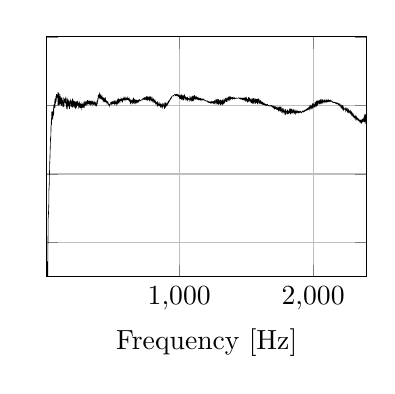
\begin{tikzpicture}

\begin{axis}[%
width=1.6in,
height=1.2in,
at={(1.011in,0.642in)},
scale only axis,
xmin=10,
xmax=2400,
xmajorgrids,
ymin=-10,
ymax=60,
ymajorgrids,
yticklabels={\empty},
xlabel={Frequency [Hz]},
axis background/.style={fill=white}
]
\addplot [color=black,solid,line width=0.2pt,forget plot]
  table[row sep=crcr]{%
0	-17.5243675804023\\
0.666675926054529	11.6908135220078\\
1.33335185210906	27.4091306010963\\
2.00002777816359	13.3933613542969\\
2.66670370421811	6.73337425753634\\
3.33337963027264	-2.21558483464182\\
4.00005555632717	1.93738295607277\\
4.6667314823817	-8.07951827689944\\
5.33340740843623	-9.48955771115387\\
6.00008333449076	-9.51261766520844\\
6.66675926054529	-9.84579827102931\\
7.33343518659981	-13.5946991303349\\
8.00011111265434	-5.13549640754086\\
8.66678703870887	-11.6527379823582\\
9.3334629647634	-8.97705169253408\\
10.0001388908179	-7.97943449610387\\
10.6668148168725	-9.05032388151381\\
11.333490742927	-9.36076574689154\\
12.0001666689815	-10.3814990955259\\
12.666842595036	-8.13691708425721\\
13.3335185210906	-9.51967996995161\\
14.0001944471451	-5.5081012882811\\
14.6668703731996	-9.76844075054212\\
15.3335462992542	-9.14627795845782\\
16.0002222253087	-10.2352912115537\\
16.6668981513632	-13.1921032030214\\
17.3335740774177	-9.36165344741177\\
18.0002500034723	-8.69574471129615\\
18.6669259295268	-14.2654179867183\\
19.3336018555813	-2.43496321922927\\
20.0002777816359	1.54233037549102\\
20.6669537076904	4.55278865504605\\
21.3336296337449	7.13417626022269\\
22.0003055597994	7.3217981006321\\
22.666981485854	7.97740494263597\\
23.3336574119085	8.618862183768\\
24.000333337963	8.47730115224057\\
24.6670092640176	8.79033451027347\\
25.3336851900721	10.085291199619\\
26.0003611161266	11.9119605978118\\
26.6670370421811	14.028467014482\\
27.3337129682357	15.6475401800129\\
28.0003888942902	16.7118373023949\\
28.6670648203447	16.9924101400291\\
29.3337407463993	16.8037476197963\\
30.0004166724538	17.1574033065858\\
30.6670925985083	18.9208568770175\\
31.3337685245628	21.1762340725631\\
32.0004444506174	22.7903586541759\\
32.6671203766719	23.6511902354569\\
33.3337963027264	23.6520331903429\\
34.000472228781	23.5354735957579\\
34.6671481548355	24.6385061305446\\
35.33382408089	26.5019532159492\\
36.0005000069445	27.5840817320101\\
36.6671759329991	27.5022472935942\\
37.3338518590536	27.1318276310872\\
38.0005277851081	28.4361946811871\\
38.6672037111627	30.3916522512457\\
39.3338796372172	31.072843181382\\
40.0005555632717	30.3575304262323\\
40.6672314893262	30.4129126202265\\
41.3339074153808	32.652451649601\\
42.0005833414353	33.9986630350736\\
42.6672592674898	33.2071255857207\\
43.3339351935444	32.1947482341864\\
44.0006111195989	34.5057132969865\\
44.6672870456534	36.2050914286601\\
45.3339629717079	35.3536860295884\\
46.0006388977625	34.2725148403043\\
46.667314823817	36.7141854791821\\
47.3339907498715	38.0234070784075\\
48.0006666759261	36.7460788422497\\
48.6673426019806	36.3109088976344\\
49.3340185280351	38.2964576251457\\
50.0006944540896	37.9351708447268\\
50.6673703801442	35.9131317650072\\
51.3340463061987	37.2605910047824\\
52.0007222322532	38.0196894650859\\
52.6673981583078	35.8816814193494\\
53.3340740843623	36.3916668378759\\
54.0007500104168	38.1468465772113\\
54.6674259364713	36.9155572613331\\
55.3341018625259	36.1722651132132\\
56.0007777885804	37.9081279945196\\
56.6674537146349	37.8686218160751\\
57.3341296406895	36.8396166391291\\
58.000805566744	37.9618219871563\\
58.6674814927985	38.5122680056605\\
59.334157418853	37.2098331816371\\
60.0008333449076	38.6982092235101\\
60.6675092709621	39.0699998655468\\
61.3341851970166	37.0969914666835\\
62.0008611230712	39.7736899882767\\
62.6675370491257	39.4113907452773\\
63.3342129751802	37.6730568230303\\
64.0008889012347	40.3393457438805\\
64.6675648272893	39.3073690081068\\
65.3342407533438	39.0687511259495\\
66.0009166793983	40.3017190242429\\
66.6675926054529	39.4736985217421\\
67.3342685315074	40.063056736731\\
68.0009444575619	40.4269806060964\\
68.6676203836164	39.479712925588\\
69.334296309671	41.2414207473229\\
70.0009722357255	40.0873193868073\\
70.66764816178	40.1159975284269\\
71.3343240878346	41.9318867656728\\
72.0010000138891	39.3421138920369\\
72.6676759399436	41.6378938319848\\
73.3343518659981	40.8868519129636\\
74.0010277920527	40.9853347998421\\
74.6677037181072	41.3496361020288\\
75.3343796441617	40.912979918899\\
76.0010555702163	42.0134001251328\\
76.6677314962708	40.6397975637034\\
77.3344074223253	42.1310447196269\\
78.0010833483798	41.8538252624342\\
78.6677592744344	41.1796942825304\\
79.3344352004889	42.7809099653344\\
80.0011111265434	41.070717306062\\
80.667787052598	42.7882046371845\\
81.3344629786525	41.4739653525233\\
82.001138904707	43.0423065159855\\
82.6678148307615	41.4686788438318\\
83.3344907568161	43.2981133216268\\
84.0011666828706	42.0797928598098\\
84.6678426089251	42.981997678409\\
85.3345185349797	42.7663073250467\\
86.0011944610342	42.8733074541268\\
86.6678703870887	42.7546496348235\\
87.3345463131432	43.1204888140978\\
88.0012222391978	42.6083261850596\\
88.6678981652523	43.1706172881356\\
89.3345740913068	42.6664997993289\\
90.0012500173614	42.9768375713759\\
90.6679259434159	42.5023257882067\\
91.3346018694704	42.8516366958317\\
92.0012777955249	42.2120887623649\\
92.6679537215795	43.101919950973\\
93.334629647634	41.3324152107473\\
94.0013055736885	43.882008830517\\
94.667981499743	40.1277297181305\\
95.3346574257976	43.9196412171279\\
96.0013333518521	40.5801647874567\\
96.6680092779066	43.0928073989672\\
97.3346852039612	41.3450930030422\\
98.0013611300157	42.8421950812629\\
98.6680370560702	41.4842757428437\\
99.3347129821248	42.1352364143998\\
100.001388908179	42.9211837902236\\
100.668064834234	39.8222178907703\\
101.334740760288	43.5889856586178\\
102.001416686343	40.2912787512725\\
102.668092612397	42.3203401260629\\
103.334768538452	42.2562519745287\\
104.001444464506	40.7558961680513\\
104.668120390561	42.4600559685578\\
105.334796316616	40.3864662315736\\
106.00147224267	42.7368203481435\\
106.668148168725	41.3953691266536\\
107.334824094779	40.2364380595683\\
108.001500020834	43.2792625581823\\
108.668175946888	40.5857157634436\\
109.334851872943	41.3563098208877\\
110.001527798997	41.7936258238135\\
110.668203725052	40.3446236394804\\
111.334879651106	42.7751584007228\\
112.001555577161	40.8930306026622\\
112.668231503215	40.6797650231633\\
113.33490742927	42.2956668959875\\
114.001583355324	41.2966052356881\\
114.668259281379	40.5474688753584\\
115.334935207433	41.6051321427285\\
116.001611133488	40.8655399994044\\
116.668287059542	42.3126091551202\\
117.334962985597	41.5010451981423\\
118.001638911652	39.9255912863956\\
118.668314837706	40.8903234449624\\
119.334990763761	42.3004475974955\\
120.001666689815	41.5081871635136\\
120.66834261587	41.4083733354334\\
121.335018541924	39.8802453352612\\
122.001694467979	40.1339905879884\\
122.668370394033	41.3501834922626\\
123.335046320088	42.3473570448245\\
124.001722246142	41.4192307709075\\
124.668398172197	41.6482372958465\\
125.335074098251	40.8700622205025\\
126.001750024306	40.5033971998025\\
126.66842595036	40.4612918992392\\
127.335101876415	41.4318609758747\\
128.001777802469	40.9435818793448\\
128.668453728524	40.6075745417749\\
129.335129654579	40.800493180831\\
130.001805580633	40.1126461798542\\
130.668481506688	39.6727533850977\\
131.335157432742	39.7100165311461\\
132.001833358797	41.2632015012783\\
132.668509284851	41.1232640096121\\
133.335185210906	41.6166511470345\\
134.00186113696	41.6969368774001\\
134.668537063015	41.8360503660889\\
135.335212989069	41.2930107661913\\
136.001888915124	40.0602429739622\\
136.668564841178	40.4374808340744\\
137.335240767233	40.027220095911\\
138.001916693287	40.1839693133721\\
138.668592619342	39.598835490238\\
139.335268545396	40.0666638084032\\
140.001944471451	41.0444664574296\\
140.668620397506	40.8526653330657\\
141.33529632356	41.1973793191331\\
142.001972249615	40.8978257802962\\
142.668648175669	41.543353603907\\
143.335324101724	41.991760162114\\
144.002000027778	41.4011973550438\\
144.668675953833	41.4620237295177\\
145.335351879887	40.9796659259278\\
146.002027805942	41.2612842975198\\
146.668703731996	41.8136614783287\\
147.335379658051	41.182953866964\\
148.002055584105	41.1353326168134\\
148.66873151016	40.7913119093088\\
149.335407436214	40.635774757988\\
150.002083362269	41.7519988419126\\
150.668759288323	41.9326581324101\\
151.335435214378	42.0050828175318\\
152.002111140433	42.1299051414336\\
152.668787066487	41.1987807516473\\
153.335462992542	41.12869233425\\
154.002138918596	41.2516247804038\\
154.668814844651	40.6678278634934\\
155.335490770705	40.6924763509873\\
156.00216669676	40.1475995121494\\
156.668842622814	39.0331033287515\\
157.335518548869	39.5348666247882\\
158.002194474923	40.3407869135781\\
158.668870400978	40.3430764644635\\
159.335546327032	40.8806742140998\\
160.002222253087	41.0680847014237\\
160.668898179141	41.020819793561\\
161.335574105196	41.9029488428055\\
162.00225003125	42.299984595512\\
162.668925957305	41.0878119529134\\
163.335601883359	39.7964246005615\\
164.002277809414	39.3288364957002\\
164.668953735469	39.2430209265027\\
165.335629661523	39.7473877085781\\
166.002305587578	40.6638085917357\\
166.668981513632	40.7552584783681\\
167.335657439687	40.7282231897644\\
168.002333365741	41.4394133934474\\
168.669009291796	41.5348934125883\\
169.33568521785	40.4016289399534\\
170.002361143905	39.8829003321493\\
170.669037069959	40.8990011071995\\
171.335712996014	41.6290284855659\\
172.002388922068	41.379811263703\\
172.669064848123	40.7964938138458\\
173.335740774177	39.9268282375041\\
174.002416700232	39.8641883788128\\
174.669092626286	40.6264938690653\\
175.335768552341	40.7379535491193\\
176.002444478396	40.0532542463073\\
176.66912040445	39.9952089322039\\
177.335796330505	40.0313688301155\\
178.002472256559	39.6547245399833\\
178.669148182614	40.1018698586037\\
179.335824108668	40.8568959137331\\
180.002500034723	39.8880983414709\\
180.669175960777	39.0054518180246\\
181.335851886832	40.7168530942596\\
182.002527812886	40.8418271523458\\
182.669203738941	39.6787683859813\\
183.335879664995	40.0133324025481\\
184.00255559105	40.824078357567\\
184.669231517104	40.8736032670145\\
185.335907443159	40.5280069138791\\
186.002583369213	40.783915846379\\
186.669259295268	40.7593264942396\\
187.335935221323	41.4925826460977\\
188.002611147377	41.4032093287464\\
188.669287073432	40.5046435072617\\
189.335962999486	41.3968976652475\\
190.002638925541	40.9467357462091\\
190.669314851595	40.6077754711988\\
191.33599077765	40.9273920306519\\
192.002666703704	39.6124120499272\\
192.669342629759	40.0889065449679\\
193.336018555813	39.7906475299528\\
194.002694481868	39.8577894523716\\
194.669370407922	40.9772987741573\\
195.336046333977	39.9968505027167\\
196.002722260031	41.4110298542021\\
196.669398186086	40.9437050285812\\
197.33607411214	41.3285166455155\\
198.002750038195	41.294622557228\\
198.66942596425	40.5441214760169\\
199.336101890304	40.1934215633097\\
200.002777816359	39.8436755107678\\
200.669453742413	39.9063866086634\\
201.336129668468	40.915799186791\\
202.002805594522	40.9451545330575\\
202.669481520577	42.0015563932875\\
203.336157446631	40.7853549008446\\
204.002833372686	41.1073117070433\\
204.66950929874	39.3492160035836\\
205.336185224795	40.4610428152822\\
206.002861150849	40.0736246759544\\
206.669537076904	41.7142770428348\\
207.336213002958	41.2595198702492\\
208.002888929013	41.5241389217514\\
208.669564855067	40.040444212553\\
209.336240781122	40.1490306228824\\
210.002916707176	40.210640387417\\
210.669592633231	41.0325254837533\\
211.336268559286	41.2496228779514\\
212.00294448534	40.9025866445358\\
212.669620411395	40.1963896983963\\
213.336296337449	40.2029570433756\\
214.002972263504	41.2984498492172\\
214.669648189558	41.0514476793741\\
215.336324115613	41.0243631316277\\
216.003000041667	39.4077378962234\\
216.669675967722	39.9873316539717\\
217.336351893776	40.3662871120573\\
218.003027819831	41.2058231301269\\
218.669703745885	40.2377771931999\\
219.33637967194	39.6697442194449\\
220.003055597994	40.8589493779728\\
220.669731524049	40.8744346861014\\
221.336407450103	41.0843657294987\\
222.003083376158	39.9752096921575\\
222.669759302213	39.7985374819515\\
223.336435228267	41.0693001056631\\
224.003111154322	40.3406495110308\\
224.669787080376	39.3974269921936\\
225.336463006431	39.6608588334591\\
226.003138932485	40.477479765741\\
226.66981485854	40.2103623108113\\
227.336490784594	38.9724522470165\\
228.003166710649	39.9504115252517\\
228.669842636703	41.0381374137004\\
229.336518562758	39.4072744817001\\
230.003194488812	39.5538291129502\\
230.669870414867	41.1938185469839\\
231.336546340921	40.1989373312349\\
232.003222266976	39.5185448987688\\
232.66989819303	40.8598881053855\\
233.336574119085	40.8698288348081\\
234.00325004514	39.4450527660098\\
234.669925971194	40.5194382897784\\
235.336601897249	41.2041526532606\\
236.003277823303	40.0123619496595\\
236.669953749358	40.0783966602059\\
237.336629675412	41.2121176949891\\
238.003305601467	40.3518801862609\\
238.669981527521	40.3025267954241\\
239.336657453576	41.1255893932309\\
240.00333337963	40.1761253903468\\
240.670009305685	40.0165047095888\\
241.336685231739	41.2964257033656\\
242.003361157794	40.5359153298807\\
242.670037083848	40.5246093682064\\
243.336713009903	40.5031939207703\\
244.003388935957	39.9838103291108\\
244.670064862012	40.8634337387071\\
245.336740788066	40.7942236992314\\
246.003416714121	39.8478113638777\\
246.670092640176	40.672451305373\\
247.33676856623	40.1027695296821\\
248.003444492285	40.1557229085058\\
248.670120418339	40.2395379106218\\
249.336796344394	39.2220699477209\\
250.003472270448	40.1170421247863\\
250.670148196503	39.7255614393629\\
251.336824122557	39.9071451260916\\
252.003500048612	39.9183994779474\\
252.670175974666	39.3777195585638\\
253.336851900721	40.134955548284\\
254.003527826775	39.8987926658396\\
254.67020375283	40.739972489367\\
255.336879678884	40.7664706092323\\
256.003555604939	40.6867481554156\\
256.670231530993	40.8171076767746\\
257.336907457048	40.199344115209\\
258.003583383103	40.2835361975774\\
258.670259309157	39.6679324620827\\
259.336935235212	39.6127943796231\\
260.003611161266	39.4061893455785\\
260.670287087321	39.3163775593603\\
261.336963013375	39.3787719827417\\
262.00363893943	39.8153019355944\\
262.670314865484	39.9297324669816\\
263.336990791539	40.173273911428\\
264.003666717593	40.2810000612314\\
264.670342643648	40.0969804900018\\
265.337018569702	39.9182757161047\\
266.003694495757	39.7413253318047\\
266.670370421811	39.3292610613363\\
267.337046347866	39.6275568683327\\
268.00372227392	39.9088218601484\\
268.670398199975	40.1757125559505\\
269.33707412603	40.1616539291471\\
270.003750052084	40.3124127104493\\
270.670425978139	39.7273216363277\\
271.337101904193	39.4891083933547\\
272.003777830248	39.2710453771494\\
272.670453756302	39.5118151416545\\
273.337129682357	39.5769860737867\\
274.003805608411	39.9599877117283\\
274.670481534466	40.0554119069238\\
275.33715746052	39.6419949019253\\
276.003833386575	39.4582603328168\\
276.670509312629	39.4684441211983\\
277.337185238684	40.2315707999451\\
278.003861164738	40.1702867530888\\
278.670537090793	40.535884200389\\
279.337213016847	40.0469683114794\\
280.003888942902	39.8538442334067\\
280.670564868956	39.4001720508423\\
281.337240795011	39.5946841672881\\
282.003916721066	40.3324378156789\\
282.67059264712	40.1551965823935\\
283.337268573175	40.1363134508213\\
284.003944499229	39.3715388784373\\
284.670620425284	39.8080008966923\\
285.337296351338	40.5344429054717\\
286.003972277393	40.6344001886244\\
286.670648203447	40.55171412025\\
287.337324129502	39.3530935221291\\
288.004000055556	39.6022533904057\\
288.670675981611	40.5834211791435\\
289.337351907665	40.8290052957396\\
290.00402783372	40.7351663440847\\
290.670703759774	39.512561563733\\
291.337379685829	39.5710233900348\\
292.004055611883	40.746349126792\\
292.670731537938	40.6257103272366\\
293.337407463993	40.3236936214067\\
294.004083390047	40.0903661854939\\
294.670759316102	40.1410451617321\\
295.337435242156	40.7041979259149\\
296.004111168211	40.2692054567658\\
296.670787094265	39.8254207050681\\
297.33746302032	40.7218349630133\\
298.004138946374	40.8057248920134\\
298.670814872429	40.2002287824332\\
299.337490798483	40.4029069326862\\
300.004166724538	40.5555837810536\\
300.670842650592	40.3895439932564\\
301.337518576647	40.3674764417409\\
302.004194502701	40.2981516437823\\
302.670870428756	40.5312092680225\\
303.33754635481	40.8519003181984\\
304.004222280865	40.5192856865446\\
304.67089820692	40.3954174417142\\
305.337574132974	40.8787733611807\\
306.004250059029	40.7811314034084\\
306.670925985083	40.2846401898865\\
307.337601911138	40.4815623422689\\
308.004277837192	40.9297550149658\\
308.670953763247	40.5519911765894\\
309.337629689301	40.266796523825\\
310.004305615356	40.8574234636305\\
310.67098154141	40.9643924713872\\
311.337657467465	40.3599176621548\\
312.004333393519	40.8103453400853\\
312.671009319574	40.818588537582\\
313.337685245628	40.6200926156467\\
314.004361171683	40.8751787827842\\
314.671037097737	40.7913871782562\\
315.337713023792	40.7038632949919\\
316.004388949847	40.8416744796302\\
316.671064875901	41.5195148037448\\
317.337740801956	40.434418340194\\
318.00441672801	40.5978545788821\\
318.671092654065	41.4870737188237\\
319.337768580119	40.4280382393586\\
320.004444506174	40.9398742486964\\
320.671120432228	41.011277903175\\
321.337796358283	40.5687120134499\\
322.004472284337	41.1535677237005\\
322.671148210392	41.1392534166801\\
323.337824136446	40.3825089462819\\
324.004500062501	40.6081214009983\\
324.671175988555	41.0043665041394\\
325.33785191461	40.474250100283\\
326.004527840664	41.2928182492747\\
326.671203766719	40.5678975334036\\
327.337879692774	40.2792600063698\\
328.004555618828	40.8888881190634\\
328.671231544883	40.7349962004124\\
329.337907470937	40.9829467754223\\
330.004583396992	41.3592086747438\\
330.671259323046	40.4589886034892\\
331.337935249101	41.2437823371151\\
332.004611175155	40.8119103026496\\
332.67128710121	40.587361783092\\
333.337963027264	41.2815629618084\\
334.004638953319	40.2657310351975\\
334.671314879373	41.3346061929239\\
335.337990805428	40.7178507337445\\
336.004666731482	40.416346301215\\
336.671342657537	41.1707062597658\\
337.338018583591	40.4152321435105\\
338.004694509646	41.3261840878259\\
338.671370435701	40.6273200004729\\
339.338046361755	40.7731165816095\\
340.00472228781	41.1706672391917\\
340.671398213864	40.5025143215955\\
341.338074139919	41.1026763463055\\
342.004750065973	40.6002923412857\\
342.671425992028	41.1788432675096\\
343.338101918082	40.2645496744641\\
344.004777844137	40.6435451647145\\
344.671453770191	40.8064574185774\\
345.338129696246	40.2683821715122\\
346.0048056223	41.2964021143696\\
346.671481548355	40.7342276217187\\
347.338157474409	40.9716924348271\\
348.004833400464	40.4587244234222\\
348.671509326518	41.2729389946947\\
349.338185252573	40.4328811339214\\
350.004861178627	41.1877942392071\\
350.671537104682	40.8440283324191\\
351.338213030737	40.4309897310788\\
352.004888956791	40.7540756190691\\
352.671564882846	40.9062963748524\\
353.3382408089	40.6144722580729\\
354.004916734955	40.4329641295205\\
354.671592661009	40.8757465309462\\
355.338268587064	40.3219055710449\\
356.004944513118	40.9469157126379\\
356.671620439173	40.2076448690441\\
357.338296365227	40.8879830870786\\
358.004972291282	40.356279766249\\
358.671648217336	40.7225208415252\\
359.338324143391	40.3560886398988\\
360.005000069445	40.6337125755157\\
360.6716759955	40.4131387464735\\
361.338351921554	40.9046815345216\\
362.005027847609	40.2349223117656\\
362.671703773664	40.7878167394701\\
363.338379699718	40.3375383658683\\
364.005055625773	40.8066335379835\\
364.671731551827	40.4088180251324\\
365.338407477882	40.8135969717416\\
366.005083403936	40.8692437558552\\
366.671759329991	40.3533304068852\\
367.338435256045	40.8392591740263\\
368.0051111821	40.4215227616746\\
368.671787108154	41.1300074060068\\
369.338463034209	40.1969638962543\\
370.005138960263	41.1835760876493\\
370.671814886318	40.0068215059268\\
371.338490812372	40.6738054946437\\
372.005166738427	40.1504030784769\\
372.671842664481	40.3918398391426\\
373.338518590536	40.2163273501982\\
374.005194516591	40.2744495192198\\
374.671870442645	40.4464921816266\\
375.3385463687	40.1414931700114\\
376.005222294754	40.6789773410948\\
376.671898220809	40.3055926033823\\
377.338574146863	40.3849718999154\\
378.005250072918	40.5867484565319\\
378.671925998972	39.8099721812339\\
379.338601925027	40.549947325752\\
380.005277851081	39.7398105502847\\
380.671953777136	40.1708701426047\\
381.33862970319	40.4552174124768\\
382.005305629245	39.813672969994\\
382.671981555299	40.8995627804331\\
383.338657481354	39.8383730603664\\
384.005333407408	40.5313576133594\\
384.672009333463	40.5237851665934\\
385.338685259517	40.0968156100229\\
386.005361185572	41.1962302640632\\
386.672037111627	40.3556603884594\\
387.338713037681	41.0774738155896\\
388.005388963736	41.0072017989591\\
388.67206488979	40.4376322009207\\
389.338740815845	41.4665161638275\\
390.005416741899	41.0053722415858\\
390.672092667954	41.3566017808725\\
391.338768594008	41.7665869085269\\
392.005444520063	41.2840911010476\\
392.672120446117	41.6239875609143\\
393.338796372172	42.1398286785301\\
394.005472298226	41.7396351611967\\
394.672148224281	42.4317879600279\\
395.338824150335	42.2953508701489\\
396.00550007639	41.9108323715782\\
396.672176002444	42.6826600821695\\
397.338851928499	42.6865291414904\\
398.005527854554	42.2806913988996\\
398.672203780608	42.8281757935179\\
399.338879706663	42.7673179006333\\
400.005555632717	42.4900840865047\\
400.672231558772	43.1284806744661\\
401.338907484826	42.9401415737963\\
402.005583410881	42.2556284584675\\
402.672259336935	43.0862448178531\\
403.33893526299	43.2228474759159\\
404.005611189044	42.4939655367471\\
404.672287115099	42.6376336729739\\
405.338963041153	43.4298133437032\\
406.005638967208	42.5643059603715\\
406.672314893262	42.3616619740041\\
407.338990819317	43.0393093915562\\
408.005666745371	43.1055227601759\\
408.672342671426	42.2447146196381\\
409.339018597481	42.5562471776589\\
410.005694523535	43.2055790347622\\
410.67237044959	42.4059999614422\\
411.339046375644	42.09446160416\\
412.005722301699	42.7803906746076\\
412.672398227753	43.0920280440926\\
413.339074153808	42.2751800715823\\
414.005750079862	41.9463259085983\\
414.672426005917	42.8010183367833\\
415.339101931971	42.6364975687802\\
416.005777858026	42.1581830270132\\
416.67245378408	42.3844513244286\\
417.339129710135	42.5498769965894\\
418.005805636189	42.3182844485176\\
418.672481562244	42.1009323100914\\
419.339157488298	42.4291997775977\\
420.005833414353	42.6977889074254\\
420.672509340407	42.246540251976\\
421.339185266462	41.7224033955026\\
422.005861192517	42.036558098543\\
422.672537118571	42.5637404840807\\
423.339213044626	42.6171272635679\\
424.00588897068	42.0347564789078\\
424.672564896735	41.6721196018628\\
425.339240822789	42.0982294834131\\
426.005916748844	42.4504488959215\\
426.672592674898	42.0205046132567\\
427.339268600953	41.7888044972062\\
428.005944527007	42.1874977030767\\
428.672620453062	42.2299547055809\\
429.339296379116	42.1823095254376\\
430.005972305171	41.9081726314032\\
430.672648231225	41.2931471203397\\
431.33932415728	41.6664538699279\\
432.006000083334	42.2198059214135\\
432.672676009389	42.2446361399335\\
433.339351935444	41.9556301024238\\
434.006027861498	41.5423337349253\\
434.672703787553	41.7222954924409\\
435.339379713607	41.9013969929597\\
436.006055639662	41.9521276882231\\
436.672731565716	41.8813049889559\\
437.339407491771	41.4602696034274\\
438.006083417825	41.256930962583\\
438.67275934388	41.2191072461851\\
439.339435269934	41.7914827254114\\
440.006111195989	41.9194408102066\\
440.672787122043	41.8699333907763\\
441.339463048098	41.401852887997\\
442.006138974152	41.2973505041818\\
442.672814900207	41.4131060423808\\
443.339490826261	41.565173132479\\
444.006166752316	41.8233131380502\\
444.672842678371	41.7293884417975\\
445.339518604425	41.8330986517373\\
446.00619453048	41.4691548228327\\
446.672870456534	41.3379068213649\\
447.339546382589	41.0901380638121\\
448.006222308643	41.3784109869886\\
448.672898234698	41.5624909735669\\
449.339574160752	41.8651098781114\\
450.006250086807	41.707613118874\\
450.672926012861	41.5411468414132\\
451.339601938916	41.2660522398865\\
452.00627786497	41.0686013889118\\
452.672953791025	40.9587315283655\\
453.339629717079	40.9796779637093\\
454.006305643134	41.1488659434399\\
454.672981569188	41.2006683001599\\
455.339657495243	41.3141142326056\\
456.006333421298	41.3233773969437\\
456.673009347352	41.3557022158673\\
457.339685273407	41.1440835681784\\
458.006361199461	41.0117789256841\\
458.673037125516	40.8855014097661\\
459.33971305157	40.8190103174771\\
460.006388977625	40.6997636916078\\
460.673064903679	40.5622894641998\\
461.339740829734	40.739040148173\\
462.006416755788	40.7436994724071\\
462.673092681843	40.9140951845362\\
463.339768607897	40.9772490205487\\
464.006444533952	40.962782173619\\
464.673120460006	41.0843777444522\\
465.339796386061	41.1506795246695\\
466.006472312115	41.1188078293224\\
466.67314823817	40.9990850461086\\
467.339824164225	41.0360383462056\\
468.006500090279	40.872997780825\\
468.673176016334	40.6169321983228\\
469.339851942388	40.6096857108217\\
470.006527868443	40.4237127175355\\
470.673203794497	40.3731037115511\\
471.339879720552	40.4570906937017\\
472.006555646606	40.3323220520328\\
472.673231572661	40.3160146775773\\
473.339907498715	40.2108608789156\\
474.00658342477	40.1515780552232\\
474.673259350824	40.2805558188191\\
475.339935276879	40.2481655169125\\
476.006611202933	40.2152784521075\\
476.673287128988	40.2069947455522\\
477.339963055042	40.1513332600471\\
478.006638981097	40.0951459932133\\
478.673314907152	40.3160816388376\\
479.339990833206	40.3004951950689\\
480.006666759261	40.0320547762211\\
480.673342685315	40.2278701327005\\
481.34001861137	40.2344914470124\\
482.006694537424	40.2732798350145\\
482.673370463479	40.2199188583452\\
483.340046389533	40.175253405523\\
484.006722315588	40.2404332446799\\
484.673398241642	40.3905000265809\\
485.340074167697	40.377029644786\\
486.006750093751	40.4281425518142\\
486.673426019806	40.4486887026317\\
487.34010194586	40.7093933579849\\
488.006777871915	40.8000216944063\\
488.673453797969	40.7469242642522\\
489.340129724024	40.8706094098165\\
490.006805650078	40.9321026667647\\
490.673481576133	40.9218442064378\\
491.340157502188	40.9164874292495\\
492.006833428242	40.9190511485929\\
492.673509354297	40.9266088012614\\
493.340185280351	40.6387254941569\\
494.006861206406	40.6123979446802\\
494.67353713246	40.3633564584399\\
495.340213058515	40.4309900529484\\
496.006888984569	40.376218869836\\
496.673564910624	40.5209817988183\\
497.340240836678	40.5568598795006\\
498.006916762733	40.7796498722443\\
498.673592688787	40.9686252202719\\
499.340268614842	40.9024040999969\\
500.006944540896	40.9759407164165\\
500.673620466951	40.9437546205872\\
501.340296393005	40.8145573506859\\
502.00697231906	40.7673342418059\\
502.673648245115	40.5251878514348\\
503.340324171169	40.4897617002641\\
504.007000097224	40.5639047660737\\
504.673676023278	40.7769545900645\\
505.340351949333	41.0667022744023\\
506.007027875387	41.1695588469684\\
506.673703801442	41.0442548205813\\
507.340379727496	40.937182234463\\
508.007055653551	40.5650306733402\\
508.673731579605	40.5671759735511\\
509.34040750566	40.6646849940156\\
510.007083431714	40.7832829607823\\
510.673759357769	41.0509603890356\\
511.340435283823	41.0388758927266\\
512.007111209878	40.9819280658606\\
512.673787135932	40.7916722851385\\
513.340463061987	40.5619522900172\\
514.007138988041	40.4740456495662\\
514.673814914096	40.725638280315\\
515.340490840151	41.0925099408709\\
516.007166766205	41.0075473266804\\
516.67384269226	40.8191452463937\\
517.340518618314	40.5084164358754\\
518.007194544369	40.4797392914654\\
518.673870470423	40.6618965486836\\
519.340546396478	40.9802708620532\\
520.007222322532	41.0567997020975\\
520.673898248587	40.8084467490751\\
521.340574174641	40.4734521724991\\
522.007250100696	40.4747155642005\\
522.67392602675	40.7792103795531\\
523.340601952805	40.9962584200235\\
524.007277878859	40.8359456964968\\
524.673953804914	40.5443700620205\\
525.340629730968	40.5107055767403\\
526.007305657023	40.7900907272846\\
526.673981583078	40.9523229433113\\
527.340657509132	40.9226470899383\\
528.007333435187	40.59507260181\\
528.674009361241	40.5329392141705\\
529.340685287296	40.8247166376132\\
530.00736121335	41.0964114931682\\
530.674037139405	40.7690259758511\\
531.340713065459	40.5107349330466\\
532.007388991514	40.7582912863268\\
532.674064917568	41.0523311526584\\
533.340740843623	40.9879973708252\\
534.007416769677	40.5767578264197\\
534.674092695732	40.5848005959617\\
535.340768621786	41.1119175757051\\
536.007444547841	41.2274223654575\\
536.674120473896	40.6841037976798\\
537.34079639995	40.6475147266054\\
538.007472326005	41.1061915355792\\
538.674148252059	41.1882089072796\\
539.340824178114	40.8746941118547\\
540.007500104168	40.8026882584127\\
540.674176030223	41.2974537414146\\
541.340851956277	41.2846939412523\\
542.007527882332	40.8172803301024\\
542.674203808386	40.9394113274808\\
543.340879734441	41.3511242689778\\
544.007555660495	41.187295977334\\
544.67423158655	40.831295803432\\
545.340907512604	41.2584759866538\\
546.007583438659	41.5593169714383\\
546.674259364713	41.0772253582425\\
547.340935290768	41.174956859112\\
548.007611216823	41.5820826044419\\
548.674287142877	41.406986566629\\
549.340963068932	41.1004115273095\\
550.007638994986	41.4834726780778\\
550.674314921041	41.5420968735367\\
551.340990847095	41.1481119795126\\
552.00766677315	41.3013697836272\\
552.674342699204	41.6172712173173\\
553.341018625259	41.2746006704668\\
554.007694551313	41.2423966723535\\
554.674370477368	41.7605082948174\\
555.341046403422	41.3125524398605\\
556.007722329477	41.3397400255568\\
556.674398255531	41.7313359309073\\
557.341074181586	41.4206941253006\\
558.00775010764	41.2906203754204\\
558.674426033695	41.8246640014946\\
559.341101959749	41.4076871182866\\
560.007777885804	41.4221858742876\\
560.674453811858	41.8678932357097\\
561.341129737913	41.4819996842292\\
562.007805663968	41.4825548780796\\
562.674481590022	41.894008847248\\
563.341157516077	41.3693109337721\\
564.007833442131	41.6427793692459\\
564.674509368186	41.820021943311\\
565.34118529424	41.3711321338662\\
566.007861220295	41.8888239872339\\
566.674537146349	41.7726517267926\\
567.341213072404	41.4706153429605\\
568.007888998458	41.8290754551559\\
568.674564924513	41.4667711105336\\
569.341240850567	41.510546934807\\
570.007916776622	41.945219729977\\
570.674592702676	41.3363785006633\\
571.341268628731	41.839169688839\\
572.007944554785	41.6490546711325\\
572.67462048084	41.5110984574394\\
573.341296406895	42.0574514314045\\
574.007972332949	41.4983885985488\\
574.674648259004	41.8589477296125\\
575.341324185058	41.6343829707858\\
576.008000111113	41.4688712120303\\
576.674676037167	42.0322031297288\\
577.341351963222	41.4807186557714\\
578.008027889276	41.9711091481978\\
578.674703815331	41.6486687373785\\
579.341379741385	41.8013220265432\\
580.00805566744	41.8661579050682\\
580.674731593494	41.5018353787776\\
581.341407519549	42.0225919479399\\
582.008083445603	41.5088146878774\\
582.674759371658	42.1043167627971\\
583.341435297712	41.4873909405656\\
584.008111223767	41.8185562721854\\
584.674787149822	41.8905636681347\\
585.341463075876	41.8123427498219\\
586.008139001931	41.9816991159336\\
586.674814927985	41.6188166459689\\
587.34149085404	42.12425378201\\
588.008166780094	41.5200441319703\\
588.674842706149	42.2108486557473\\
589.341518632203	41.5701611745434\\
590.008194558258	42.0722423761621\\
590.674870484312	41.6328132858516\\
591.341546410367	42.1223920014267\\
592.008222336421	41.6632304785111\\
592.674898262476	41.9644480040885\\
593.34157418853	41.8384478102789\\
594.008250114585	42.0299468334175\\
594.674926040639	41.8322665814657\\
595.341601966694	41.9210967328056\\
596.008277892749	41.9537306113863\\
596.674953818803	41.9487770963965\\
597.341629744858	41.8631736151987\\
598.008305670912	41.9980539050077\\
598.674981596967	41.99342745513\\
599.341657523021	41.861440099138\\
600.008333449076	41.9118437168328\\
600.67500937513	42.0574281710169\\
601.341685301185	41.8608310286355\\
602.008361227239	42.1272003267646\\
602.675037153294	41.7804835658434\\
603.341713079348	42.1155054051905\\
604.008389005403	41.7282352243452\\
604.675064931457	42.2555696156458\\
605.341740857512	41.714594660155\\
606.008416783566	42.2306210417487\\
606.675092709621	41.710295085102\\
607.341768635676	42.2185300325116\\
608.00844456173	41.774712356172\\
608.675120487785	42.1481547635246\\
609.341796413839	41.8868498681302\\
610.008472339894	41.9711395420684\\
610.675148265948	42.1032899585861\\
611.341824192003	41.7440422867758\\
612.008500118057	42.2492862873757\\
612.675176044112	41.6087939739299\\
613.341851970166	42.1883572841801\\
614.008527896221	41.6773671679444\\
614.675203822275	41.9989941444717\\
615.34187974833	42.0131509732215\\
616.008555674384	41.7691858307595\\
616.675231600439	42.2258729674475\\
617.341907526493	41.5982788592339\\
618.008583452548	42.1152912256774\\
618.675259378603	41.7384725743184\\
619.341935304657	41.7849625941665\\
620.008611230711	42.0664551748826\\
620.675287156766	41.5044126630331\\
621.341963082821	42.146631548977\\
622.008639008875	41.5629185532038\\
622.67531493493	41.8245958114845\\
623.341990860984	41.8828789026407\\
624.008666787039	41.4950637019256\\
624.675342713093	41.9676288209671\\
625.342018639148	41.6213882863405\\
626.008694565202	41.5302785639185\\
626.675370491257	41.8716005604736\\
627.342046417311	41.2964891098134\\
628.008722343366	41.7700629810545\\
628.67539826942	41.6273729074852\\
629.342074195475	41.3257450392521\\
630.008750121529	41.736556057416\\
630.675426047584	41.4954661740373\\
631.342101973638	41.2790134001158\\
632.008777899693	41.7432934898973\\
632.675453825748	41.2593704055551\\
633.342129751802	41.3617458751053\\
634.008805677857	41.607105223716\\
634.675481603911	41.1598889131601\\
635.342157529966	41.3047614395109\\
636.00883345602	41.5046680708244\\
636.675509382075	41.0630080285966\\
637.342185308129	41.1995021193986\\
638.008861234184	41.4248405260459\\
638.675537160238	40.9774642252949\\
639.342213086293	41.1922755096387\\
640.008889012347	41.3574268357799\\
640.675564938402	40.9390421257097\\
641.342240864456	41.0912080288951\\
642.008916790511	41.3209900652071\\
642.675592716565	40.9977567122516\\
643.34226864262	41.0125266357929\\
644.008944568675	41.3825445172323\\
644.675620494729	41.0776815784904\\
645.342296420784	40.8635343705104\\
646.008972346838	41.3292689480139\\
646.675648272893	41.3171066731355\\
647.342324198947	40.9217759010486\\
648.009000125002	41.1443723490413\\
648.675676051056	41.4731718631791\\
649.342351977111	41.1962433006157\\
650.009027903165	40.9591083623341\\
650.67570382922	41.4551464795126\\
651.342379755274	41.5257310535562\\
652.009055681329	41.0580019473505\\
652.675731607383	41.1970987623976\\
653.342407533438	41.5853263697607\\
654.009083459492	41.3683286905857\\
654.675759385547	41.1317480087874\\
655.342435311602	41.3131866227373\\
656.009111237656	41.5517665547303\\
656.675787163711	41.3918220163748\\
657.342463089765	41.0664437202824\\
658.00913901582	41.3777655147154\\
658.675814941874	41.6516477021685\\
659.342490867929	41.4157557760047\\
660.009166793983	41.0540556497039\\
660.675842720038	41.217631102038\\
661.342518646092	41.6245352213431\\
662.009194572147	41.5187179305886\\
662.675870498201	41.1757070966694\\
663.342546424256	41.1479643157695\\
664.00922235031	41.4562841627287\\
664.675898276365	41.5424987556222\\
665.342574202419	41.2703726845231\\
666.009250128474	41.0340079995952\\
666.675926054529	41.229773250898\\
667.342601980583	41.5673072684755\\
668.009277906638	41.5428818738239\\
668.675953832692	41.1745030304279\\
669.342629758747	41.0121620607037\\
670.009305684801	41.258704343086\\
670.675981610856	41.49387102781\\
671.34265753691	41.4566328577118\\
672.009333462965	41.1489312388881\\
672.676009389019	40.9598627820276\\
673.342685315074	41.1206128937041\\
674.009361241128	41.3677240141453\\
674.676037167183	41.4721953108148\\
675.342713093237	41.3651500826844\\
676.009389019292	41.0317216809857\\
676.676064945346	40.9731358200701\\
677.342740871401	41.0914871109846\\
678.009416797456	41.4221487416996\\
678.67609272351	41.4791628973322\\
679.342768649565	41.3079878293756\\
680.009444575619	41.0448092954206\\
680.676120501674	40.9335413897534\\
681.342796427728	41.0598009864176\\
682.009472353783	41.2758889475127\\
682.676148279837	41.4361244760996\\
683.342824205892	41.415449509122\\
684.009500131946	41.2309059175706\\
684.676176058001	40.9829610690395\\
685.342851984055	40.9540302920693\\
686.00952791011	41.0439264372488\\
686.676203836164	41.1721192292376\\
687.342879762219	41.397962684121\\
688.009555688273	41.4428404419205\\
688.676231614328	41.3701561186293\\
689.342907540382	41.2488980666267\\
690.009583466437	41.0547058168686\\
690.676259392492	40.9204606725237\\
691.342935318546	40.9618889115608\\
692.009611244601	41.0899934820624\\
692.676287170655	41.2442761052283\\
693.34296309671	41.4060015356906\\
694.009639022764	41.5340738968079\\
694.676314948819	41.4908259664472\\
695.342990874873	41.384234766109\\
696.009666800928	41.2820387429904\\
696.676342726982	41.1516280756739\\
697.343018653037	41.063486437731\\
698.009694579091	41.0345689953024\\
698.676370505146	41.1013408187333\\
699.3430464312	41.2045489474812\\
700.009722357255	41.3317448319569\\
700.676398283309	41.4841760770535\\
701.343074209364	41.5655229611814\\
702.009750135419	41.6735883740575\\
702.676426061473	41.7039064351763\\
703.343101987528	41.6597931368483\\
704.009777913582	41.6663373098612\\
704.676453839637	41.602239868675\\
705.343129765691	41.5753442470755\\
706.009805691746	41.524700289235\\
706.6764816178	41.4412034245581\\
707.343157543855	41.4067099934937\\
708.009833469909	41.3562111730384\\
708.676509395964	41.3728273927807\\
709.343185322018	41.352942649446\\
710.009861248073	41.3978693319985\\
710.676537174127	41.388752572588\\
711.343213100182	41.3903972751006\\
712.009889026236	41.4139605760255\\
712.676564952291	41.4704289987623\\
713.343240878346	41.4954054599986\\
714.0099168044	41.5123345909457\\
714.676592730455	41.541105629927\\
715.343268656509	41.5748289019563\\
716.009944582564	41.6216134159231\\
716.676620508618	41.5830624360386\\
717.343296434673	41.6170577936686\\
718.009972360727	41.6072891783439\\
718.676648286782	41.6357201671029\\
719.343324212836	41.6251065704111\\
720.010000138891	41.6155546894718\\
720.676676064945	41.6082470651803\\
721.343351991	41.6052839307068\\
722.010027917054	41.6029414770146\\
722.676703843109	41.6248403995006\\
723.343379769163	41.6380006244415\\
724.010055695218	41.6092581806152\\
724.676731621273	41.6471945227861\\
725.343407547327	41.6579508227024\\
726.010083473382	41.705724107997\\
726.676759399436	41.7590855346676\\
727.343435325491	41.8322343832971\\
728.010111251545	41.913266652305\\
728.6767871776	41.957815256644\\
729.343463103654	42.0683581237957\\
730.010139029709	42.0805530512726\\
730.676814955763	42.1696217525903\\
731.343490881818	42.1565731503252\\
732.010166807872	42.1524501350067\\
732.676842733927	42.1060860765155\\
733.343518659981	41.9943890137838\\
734.010194586036	41.9100983917674\\
734.67687051209	41.7949560609573\\
735.343546438145	41.7175803428468\\
736.0102223642	41.7139084800831\\
736.676898290254	41.7437324358657\\
737.343574216309	41.8533886594696\\
738.010250142363	42.0102625424147\\
738.676926068418	42.1094393365016\\
739.343601994472	42.2459650196354\\
740.010277920527	42.2136080908413\\
740.676953846581	42.1581938846556\\
741.343629772636	42.025706155294\\
742.01030569869	41.856720425443\\
742.676981624745	41.7878147645444\\
743.343657550799	41.8245630581606\\
744.010333476854	41.9366278945363\\
744.677009402908	42.1072332221693\\
745.343685328963	42.241069627187\\
746.010361255017	42.2554071327089\\
746.677037181072	42.1899406759233\\
747.343713107127	42.0762806837425\\
748.010389033181	41.9168609394745\\
748.677064959236	41.834288462698\\
749.34374088529	41.9570874295522\\
750.010416811345	42.140518628698\\
750.677092737399	42.2642016732177\\
751.343768663454	42.3310511821846\\
752.010444589508	42.1559343747261\\
752.677120515563	41.9127948858644\\
753.343796441617	41.8278401461423\\
754.010472367672	41.9922025672755\\
754.677148293726	42.2406268619681\\
755.343824219781	42.3436082751486\\
756.010500145835	42.213020768971\\
756.67717607189	42.0082972510594\\
757.343851997944	41.8951110330895\\
758.010527923999	42.0021425014979\\
758.677203850054	42.2052011197949\\
759.343879776108	42.3166903586018\\
760.010555702162	42.2423299078323\\
760.677231628217	41.9638397766911\\
761.343907554272	41.8331125970676\\
762.010583480326	42.0646041393277\\
762.677259406381	42.3278081999866\\
763.343935332435	42.2502919338101\\
764.01061125849	41.9862525780849\\
764.677287184544	41.8678050717621\\
765.343963110599	42.0390748833471\\
766.010639036653	42.290111258806\\
766.677314962708	42.2384877985041\\
767.343990888762	41.9090852436026\\
768.010666814817	41.8337651784772\\
768.677342740871	42.0926459859587\\
769.344018666926	42.2613235141678\\
770.01069459298	42.1180813080285\\
770.677370519035	41.845489956015\\
771.344046445089	41.8728193040165\\
772.010722371144	42.1945943216676\\
772.677398297199	42.1792903271695\\
773.344074223253	41.8752615144069\\
774.010750149308	41.8307301285393\\
774.677426075362	42.0969279212908\\
775.344102001417	42.1963471815389\\
776.010777927471	41.8856082234884\\
776.677453853526	41.7799007118387\\
777.34412977958	42.0792384600643\\
778.010805705635	42.1589792133968\\
778.677481631689	41.8978776559736\\
779.344157557744	41.7529582333936\\
780.010833483798	42.0952613581086\\
780.677509409853	42.1633176096305\\
781.344185335907	41.8143215488657\\
782.010861261962	41.8096691410514\\
782.677537188016	42.1104965420758\\
783.344213114071	42.0037546757649\\
784.010889040126	41.6993883706523\\
784.67756496618	41.9479534460089\\
785.344240892235	42.1043669332665\\
786.010916818289	41.8599948571\\
786.677592744344	41.7446494393008\\
787.344268670398	42.0959081194141\\
788.010944596453	41.973372453474\\
788.677620522507	41.7152166063224\\
789.344296448562	41.9575125649736\\
790.010972374616	42.0572413465553\\
790.677648300671	41.7077819024081\\
791.344324226725	41.8446398611917\\
792.01100015278	42.0097666100578\\
792.677676078834	41.7305706163631\\
793.344352004889	41.7066718299445\\
794.011027930943	41.9993245371116\\
794.677703856998	41.7336434839973\\
795.344379783053	41.6376231623715\\
796.011055709107	41.9761171771098\\
796.677731635162	41.6756984271754\\
797.344407561216	41.6295071195545\\
798.011083487271	41.9023578000802\\
798.677759413325	41.6457547496462\\
799.34443533938	41.5611496453537\\
800.011111265434	41.8530010141523\\
800.677787191489	41.5282783685476\\
801.344463117543	41.559813059117\\
802.011139043598	41.7663096151338\\
802.677814969652	41.4304989663944\\
803.344490895707	41.5676488986664\\
804.011166821761	41.6671489883383\\
804.677842747816	41.3094958378136\\
805.34451867387	41.5855082569095\\
806.011194599925	41.4688602555386\\
806.67787052598	41.2524824167345\\
807.344546452034	41.5813533084468\\
808.011222378089	41.2394893971091\\
808.677898304143	41.3502244871889\\
809.344574230198	41.4838865461923\\
810.011250156252	41.0835790219834\\
810.677926082307	41.4635180602725\\
811.344602008361	41.2092661764441\\
812.011277934416	41.1474127241603\\
812.67795386047	41.4014653293046\\
813.344629786525	40.9991595150213\\
814.011305712579	41.3495190105942\\
814.677981638634	41.0937345653149\\
815.344657564688	41.11228392437\\
816.011333490743	41.266072067988\\
816.678009416797	40.8489982632076\\
817.344685342852	41.2413425667051\\
818.011361268907	40.8736642490883\\
818.678037194961	41.1285204938854\\
819.344713121016	41.0435814395293\\
820.01138904707	40.8797476675945\\
820.678064973125	41.135360301072\\
821.344740899179	40.7321775899997\\
822.011416825234	41.1442407073504\\
822.678092751288	40.729875353929\\
823.344768677343	41.0234920743962\\
824.011444603397	40.8224404150879\\
824.678120529452	40.846664050533\\
825.344796455506	40.9004720785369\\
826.011472381561	40.7170509653856\\
826.678148307615	40.9400961427617\\
827.34482423367	40.6078851322505\\
828.011500159724	40.9601774461112\\
828.678176085779	40.5277914086113\\
829.344852011833	40.910655322659\\
830.011527937888	40.4801209627691\\
830.678203863943	40.858415882434\\
831.344879789997	40.4634825807967\\
832.011555716052	40.7234123738469\\
832.678231642106	40.4406899661651\\
833.344907568161	40.7280771371353\\
834.011583494215	40.4524876909185\\
834.67825942027	40.6546609807126\\
835.344935346324	40.3995892793999\\
836.011611272379	40.5926635543192\\
836.678287198433	40.4017809927979\\
837.344963124488	40.502357920454\\
838.011639050542	40.3372407611015\\
838.678314976597	40.5211114710354\\
839.344990902651	40.2779198920954\\
840.011666828706	40.5156192213903\\
840.67834275476	40.1969054522558\\
841.345018680815	40.5188562474541\\
842.01169460687	40.1567639298478\\
842.678370532924	40.499720945209\\
843.345046458979	40.1224552285362\\
844.011722385033	40.5076382229382\\
844.678398311088	40.0386394270286\\
845.345074237142	40.4883774824313\\
846.011750163197	40.0812091612959\\
846.678426089251	40.3544819730077\\
847.345102015306	40.1735650271761\\
848.01177794136	40.2615706686619\\
848.678453867415	40.2428161567462\\
849.345129793469	40.1073306581026\\
850.011805719524	40.3800126384481\\
850.678481645578	39.9828268571112\\
851.345157571633	40.3917633813483\\
852.011833497687	39.9990628690795\\
852.678509423742	40.2879841385656\\
853.345185349797	40.111113926133\\
854.011861275851	40.1061673375863\\
854.678537201906	40.2523040525641\\
855.34521312796	39.9212739166394\\
856.011889054015	40.3518256624123\\
856.678564980069	39.9485695034608\\
857.345240906124	40.2151915863751\\
858.011916832178	40.1520338736915\\
858.678592758233	39.9903449822081\\
859.345268684287	40.3509427387288\\
860.011944610342	39.8712296142408\\
860.678620536396	40.2282964835048\\
861.345296462451	40.1074124811468\\
862.011972388505	39.957685913686\\
862.67864831456	40.3055923750484\\
863.345324240614	39.8732553178969\\
864.012000166669	40.1418841575489\\
864.678676092724	40.1683709864818\\
865.345352018778	39.8597669146264\\
866.012027944833	40.2312391794969\\
866.678703870887	39.9266061591095\\
867.345379796942	39.9524496257107\\
868.012055722996	40.2249418556613\\
868.678731649051	39.8642427220566\\
869.345407575105	40.0311126770589\\
870.01208350116	40.132292905506\\
870.678759427214	39.7574720742639\\
871.345435353269	40.1403397381791\\
872.012111279323	40.0453600479588\\
872.678787205378	39.7625331377639\\
873.345463131432	40.1310230911087\\
874.012139057487	39.9595272725259\\
874.678814983541	39.7819074901937\\
875.345490909596	40.1585541455671\\
876.012166835651	39.9175972830856\\
876.678842761705	39.759064393566\\
877.34551868776	40.1491920425223\\
878.012194613814	39.9172386647969\\
878.678870539869	39.7101982769757\\
879.345546465923	40.0868325069406\\
880.012222391978	39.9778956085192\\
880.678898318032	39.715148943231\\
881.345574244087	40.0503277672599\\
882.012250170141	40.0858229801438\\
882.678926096196	39.7110005147543\\
883.34560202225	39.9823676766057\\
884.012277948305	40.1089732687676\\
884.678953874359	39.7909108761659\\
885.345629800414	39.8037921176846\\
886.012305726468	40.142136369437\\
886.678981652523	39.9216719604003\\
887.345657578578	39.7263360337945\\
888.012333504632	40.0795358424263\\
888.679009430687	40.0858609099766\\
889.345685356741	39.7914021389145\\
890.012361282796	39.8953434119215\\
890.67903720885	40.1852610657068\\
891.345713134905	40.0372888169502\\
892.012389060959	39.7865233279454\\
892.679064987014	40.0506845591864\\
893.345740913068	40.2331879825119\\
894.012416839123	40.0106295169553\\
894.679092765177	39.844949649926\\
895.345768691232	40.1158019750392\\
896.012444617286	40.2729080688641\\
896.679120543341	40.0290037684233\\
897.345796469395	39.8952424937685\\
898.01247239545	40.1703898788118\\
898.679148321504	40.3128948782728\\
899.345824247559	40.1055353132793\\
900.012500173613	39.9758267568282\\
900.679176099668	40.1321130169962\\
901.345852025723	40.3846014446669\\
902.012527951777	40.2741176313502\\
902.679203877832	40.0175397161473\\
903.345879803886	40.0972350422149\\
904.012555729941	40.3795544935746\\
904.679231655995	40.4088693423851\\
905.34590758205	40.2256640923708\\
906.012583508104	40.1200274840959\\
906.679259434159	40.2464803396646\\
907.345935360213	40.4993712430744\\
908.012611286268	40.5495538696252\\
908.679287212322	40.3314633991627\\
909.345963138377	40.2223425394787\\
910.012639064431	40.4175584044116\\
910.679314990486	40.6591165362352\\
911.34599091654	40.6678722448505\\
912.012666842595	40.5211920005775\\
912.67934276865	40.3870023767044\\
913.346018694704	40.48185802262\\
914.012694620759	40.68161063626\\
914.679370546813	40.8654908407279\\
915.346046472868	40.8211157957737\\
916.012722398922	40.6408240836734\\
916.679398324977	40.5596306193844\\
917.346074251031	40.6832167322689\\
918.012750177086	40.9588809451612\\
918.67942610314	41.0815763313869\\
919.346102029195	41.0480418997538\\
920.012777955249	40.9343276868352\\
920.679453881304	40.8354714168817\\
921.346129807358	40.8607227404487\\
922.012805733413	41.0321511506028\\
922.679481659467	41.232751902023\\
923.346157585522	41.3940695182901\\
924.012833511577	41.3755452547923\\
924.679509437631	41.2408204929886\\
925.346185363686	41.1217470483702\\
926.01286128974	41.1232697417551\\
926.679537215795	41.2753816690067\\
927.346213141849	41.4839455119098\\
928.012889067904	41.6316586985553\\
928.679564993958	41.6861318874277\\
929.346240920013	41.6856164227384\\
930.012916846067	41.6581992212917\\
930.679592772122	41.5622529974249\\
931.346268698176	41.5469412898446\\
932.012944624231	41.5652028289216\\
932.679620550285	41.6258857336152\\
933.34629647634	41.7772100196909\\
934.012972402394	41.9717894871754\\
934.679648328449	42.0780910693078\\
935.346324254504	42.1193245006173\\
936.013000180558	42.1387719676786\\
936.679676106613	42.1605812117515\\
937.346352032667	42.1171369812031\\
938.013027958722	42.0232191241085\\
938.679703884776	41.9636812811432\\
939.346379810831	41.9941535442697\\
940.013055736885	42.0437486465642\\
940.67973166294	42.0967112466695\\
941.346407588994	42.1644447235671\\
942.013083515049	42.2974875418328\\
942.679759441103	42.4666415367708\\
943.346435367158	42.5117343406482\\
944.013111293212	42.5746892582331\\
944.679787219267	42.6413779652497\\
945.346463145321	42.7019755836698\\
946.013139071376	42.694087078752\\
946.679814997431	42.7300898962303\\
947.346490923485	42.7577456543621\\
948.01316684954	42.7205811593358\\
948.679842775594	42.7043374160567\\
949.346518701649	42.7205202961524\\
950.013194627703	42.7211019400414\\
950.679870553758	42.7121993916793\\
951.346546479812	42.7231354244724\\
952.013222405867	42.744660328976\\
952.679898331921	42.7115685709616\\
953.346574257976	42.7123582170731\\
954.01325018403	42.7629236870613\\
954.679926110085	42.7365738450653\\
955.346602036139	42.7501578677945\\
956.013277962194	42.8236553456758\\
956.679953888248	42.8061890891494\\
957.346629814303	42.8172723325829\\
958.013305740358	42.882171763966\\
958.679981666412	42.8636181695432\\
959.346657592467	42.894763186467\\
960.013333518521	42.9484617141619\\
960.680009444576	42.9386524153271\\
961.34668537063	42.9846594967157\\
962.013361296685	43.0327583716334\\
962.680037222739	43.0248809456632\\
963.346713148794	43.0957859453517\\
964.013389074848	43.113648202736\\
964.680065000903	43.1283105601763\\
965.346740926957	43.2154181254049\\
966.013416853012	43.1846984849238\\
966.680092779066	43.2284695192107\\
967.346768705121	43.225798527785\\
968.013444631175	43.1787713842494\\
968.68012055723	43.1748095418139\\
969.346796483284	43.0987553658867\\
970.013472409339	43.0577324563093\\
970.680148335394	43.0054988034064\\
971.346824261448	42.9144314965985\\
972.013500187503	42.9344596478592\\
972.680176113557	42.8783643772689\\
973.346852039612	42.9733165398198\\
974.013527965666	42.974763049534\\
974.680203891721	43.098616198363\\
975.346879817775	43.1565127651019\\
976.01355574383	43.2106622107782\\
976.680231669884	43.2436477463347\\
977.346907595939	43.1828700488736\\
978.013583521993	43.1416258993595\\
978.680259448048	43.0043865103258\\
979.346935374102	42.9733271570105\\
980.013611300157	42.8775927114691\\
980.680287226211	42.9176283885167\\
981.346963152266	42.9385694666905\\
982.013639078321	43.0656472112803\\
982.680315004375	43.1258606808357\\
983.34699093043	43.1994861943686\\
984.013666856484	43.1543733093588\\
984.680342782539	43.0458893083606\\
985.347018708593	42.8975011775865\\
986.013694634648	42.8211826598821\\
986.680370560702	42.825694154004\\
987.347046486757	42.9559797227719\\
988.013722412811	43.0712366255274\\
988.680398338866	43.1404427464357\\
989.34707426492	43.0330175835182\\
990.013750190975	42.9174680328703\\
990.680426117029	42.7530110805106\\
991.347102043084	42.7719535031426\\
992.013777969138	42.8523095047834\\
992.680453895193	43.0337682043194\\
993.347129821248	43.0226000462881\\
994.013805747302	42.964130378448\\
994.680481673357	42.736826512564\\
995.347157599411	42.6628127852969\\
996.013833525466	42.7364791877807\\
996.68050945152	42.8842732316296\\
997.347185377575	42.970317451254\\
998.013861303629	42.849486487465\\
998.680537229684	42.6664331361535\\
999.347213155738	42.5535131850698\\
1000.01388908179	42.7363606734622\\
1000.68056500785	42.864972868276\\
1001.3472409339	42.8166995580169\\
1002.01391685996	42.6586578058097\\
1002.68059278601	42.4685614874904\\
1003.34726871207	42.5884540890453\\
1004.01394463812	42.7768058291646\\
1004.68062056417	42.7914748918424\\
1005.34729649023	42.5818323088719\\
1006.01397241628	42.3925138324511\\
1006.68064834234	42.5624468188717\\
1007.34732426839	42.7304753252444\\
1008.01400019445	42.6744839154026\\
1008.6806761205	42.4612784417713\\
1009.34735204656	42.3381364633116\\
1010.01402797261	42.6083984764296\\
1010.68070389867	42.7191258731464\\
1011.34737982472	42.4444846783146\\
1012.01405575077	42.3292171128463\\
1012.68073167683	42.4619141105228\\
1013.34740760288	42.6330813760462\\
1014.01408352894	42.5449602099774\\
1014.68075945499	42.2404822045274\\
1015.34743538105	42.3689462642313\\
1016.0141113071	42.6196862291294\\
1016.68078723316	42.4816304987554\\
1017.34746315921	42.2240905432593\\
1018.01413908527	42.3540819985573\\
1018.68081501132	42.5930394477658\\
1019.34749093737	42.3694498610328\\
1020.01416686343	42.193461931044\\
1020.68084278948	42.4097663061507\\
1021.34751871554	42.520099209337\\
1022.01419464159	42.247619990658\\
1022.68087056765	42.2252942592452\\
1023.3475464937	42.4712330897052\\
1024.01422241976	42.4353166177743\\
1024.68089834581	42.1578768977919\\
1025.34757427186	42.3479377862254\\
1026.01425019792	42.4831907893703\\
1026.68092612397	42.2073380356029\\
1027.34760205003	42.1934590772814\\
1028.01427797608	42.4817246700166\\
1028.68095390214	42.3222345443816\\
1029.34762982819	42.1334787297811\\
1030.01430575425	42.4392071545779\\
1030.6809816803	42.41594565137\\
1031.34765760636	42.0880992241028\\
1032.01433353241	42.3512030381002\\
1032.68100945846	42.474152630574\\
1033.34768538452	42.1266292969568\\
1034.01436131057	42.2816001857498\\
1034.68103723663	42.4536799036944\\
1035.34771316268	42.1745919764748\\
1036.01438908874	42.30383506317\\
1036.68106501479	42.4786511118743\\
1037.34774094085	42.1048388761819\\
1038.0144168669	42.3491912387104\\
1038.68109279296	42.4771151314975\\
1039.34776871901	42.1318284023872\\
1040.01444464506	42.3694132280306\\
1040.68112057112	42.3947386856658\\
1041.34779649717	42.1015330831287\\
1042.01447242323	42.4794290187493\\
1042.68114834928	42.3068212725986\\
1043.34782427534	42.1342823469145\\
1044.01450020139	42.4623903136899\\
1044.68117612745	42.1604729740195\\
1045.3478520535	42.2534072108511\\
1046.01452797956	42.4599285066211\\
1046.68120390561	42.0778953782524\\
1047.34787983166	42.3510038316568\\
1048.01455575772	42.2771945041241\\
1048.68123168377	42.0739870715149\\
1049.34790760983	42.4343363586829\\
1050.01458353588	42.1094277130273\\
1050.68125946194	42.2743480237354\\
1051.34793538799	42.2900162017812\\
1052.01461131405	42.0417042823863\\
1052.6812872401	42.3655991287113\\
1053.34796316616	42.0026455929879\\
1054.01463909221	42.2337593686145\\
1054.68131501826	42.2300463089035\\
1055.34799094432	42.0340534828168\\
1056.01466687037	42.3119750742708\\
1056.68134279643	41.9438132244024\\
1057.34801872248	42.2554564244159\\
1058.01469464854	42.0028727407349\\
1058.68137057459	42.0720767947323\\
1059.34804650065	42.1306286743161\\
1060.0147224267	41.9520488732335\\
1060.68139835275	42.254115792924\\
1061.34807427881	41.8750648387608\\
1062.01475020486	42.2257423439953\\
1062.68142613092	41.9178845788629\\
1063.34810205697	42.1311039305027\\
1064.01477798303	42.0034255297107\\
1064.68145390908	41.9997808598413\\
1065.34812983514	42.0473697292163\\
1066.01480576119	41.8747820635041\\
1066.68148168725	42.1338951536576\\
1067.3481576133	41.7977660850519\\
1068.01483353935	42.134435360801\\
1068.68150946541	41.764298957357\\
1069.34818539146	42.0987789899058\\
1070.01486131752	41.7286288160085\\
1070.68153724357	42.0950413799428\\
1071.34821316963	41.7593306992046\\
1072.01488909568	42.0582969174279\\
1072.68156502174	41.7623282573049\\
1073.34824094779	42.0650697095533\\
1074.01491687385	41.7826534738173\\
1074.6815927999	42.0233623927546\\
1075.34826872595	41.7609576755376\\
1076.01494465201	42.0133687817409\\
1076.68162057806	41.7315994784589\\
1077.34829650412	41.9991026261773\\
1078.01497243017	41.7337210926009\\
1078.68164835623	42.0243503531217\\
1079.34832428228	41.7157045509364\\
1080.01500020834	42.0338426605305\\
1080.68167613439	41.6992555395142\\
1081.34835206045	42.0517178389905\\
1082.0150279865	41.7137277776335\\
1082.68170391255	42.0430024658069\\
1083.34837983861	41.7313933165411\\
1084.01505576466	42.0126745446707\\
1084.68173169072	41.7935242907869\\
1085.34840761677	41.9802487355118\\
1086.01508354283	41.9047524090689\\
1086.68175946888	41.8866430918723\\
1087.34843539494	41.9890807497962\\
1088.01511132099	41.8260343958879\\
1088.68178724705	42.0982797608745\\
1089.3484631731	41.7840152194257\\
1090.01513909915	42.0851952634552\\
1090.68181502521	41.7949353395584\\
1091.34849095126	41.9786030996653\\
1092.01516687732	41.8964115014507\\
1092.68184280337	41.8749083659477\\
1093.34851872943	42.0550947163764\\
1094.01519465548	41.7951240426587\\
1094.68187058154	42.1148571305509\\
1095.34854650759	41.85270889096\\
1096.01522243365	42.0128237029591\\
1096.6818983597	42.0170808768653\\
1097.34857428575	41.8848901698352\\
1098.01525021181	42.131311120594\\
1098.68192613786	41.8740780538686\\
1099.34860206392	42.0960520623391\\
1100.01527798997	42.0341805852999\\
1100.68195391603	41.9388636596162\\
1101.34862984208	42.1604185259489\\
1102.01530576814	41.912703603874\\
1102.68198169419	42.086984213965\\
1103.34865762024	42.0908704413398\\
1104.0153335463	41.9502015117108\\
1104.68200947235	42.2119900233238\\
1105.34868539841	42.0201206347177\\
1106.01536132446	42.0721785900038\\
1106.68203725052	42.227064351353\\
1107.34871317657	41.9952086597548\\
1108.01538910263	42.1876241912901\\
1108.68206502868	42.209378400272\\
1109.34874095474	42.011234211272\\
1110.01541688079	42.2540628736426\\
1110.68209280684	42.1644501978621\\
1111.3487687329	42.0545893647728\\
1112.01544465895	42.3154099944228\\
1112.68212058501	42.1339461785704\\
1113.34879651106	42.1039842274499\\
1114.01547243712	42.3243859253428\\
1114.68214836317	42.1365753845441\\
1115.34882428923	42.148590838404\\
1116.01550021528	42.3612637202945\\
1116.68217614134	42.1564811163802\\
1117.34885206739	42.1194649685638\\
1118.01552799344	42.3757957997746\\
1118.6822039195	42.2195252622252\\
1119.34887984555	42.1333734795714\\
1120.01555577161	42.3362206724184\\
1120.68223169766	42.2772459604317\\
1121.34890762372	42.1391636692371\\
1122.01558354977	42.3259853753568\\
1122.68225947583	42.3075245154145\\
1123.34893540188	42.1511384212423\\
1124.01561132794	42.267094669132\\
1124.68228725399	42.3551995141723\\
1125.34896318004	42.1731115385795\\
1126.0156391061	42.1621445285627\\
1126.68231503215	42.3506622805454\\
1127.34899095821	42.2471071914409\\
1128.01566688426	42.0900598829418\\
1128.68234281032	42.2444138684317\\
1129.34901873637	42.3485967916678\\
1130.01569466243	42.1295978261324\\
1130.68237058848	42.1207023707622\\
1131.34904651453	42.2981477701365\\
1132.01572244059	42.2770794311877\\
1132.68239836664	42.1043069111978\\
1133.3490742927	42.0615792693859\\
1134.01575021875	42.2724979401386\\
1134.68242614481	42.227594566486\\
1135.34910207086	41.9949346980112\\
1136.01577799692	42.0743772524708\\
1136.68245392297	42.2435380890692\\
1137.34912984903	42.2037367069602\\
1138.01580577508	41.9669088801174\\
1138.68248170113	41.9917176940682\\
1139.34915762719	42.1527589272012\\
1140.01583355324	42.1511102253329\\
1140.6825094793	41.992539405497\\
1141.34918540535	41.8751651161433\\
1142.01586133141	42.0567412218877\\
1142.68253725746	42.1322015161221\\
1143.34921318352	42.0108319826583\\
1144.01588910957	41.8232900727781\\
1144.68256503563	41.8814597258183\\
1145.34924096168	42.0307274481744\\
1146.01591688773	42.0816469857228\\
1146.68259281379	41.8741067237521\\
1147.34926873984	41.7809856322674\\
1148.0159446659	41.7958002032343\\
1148.68262059195	41.9966201327332\\
1149.34929651801	42.0177059445414\\
1150.01597244406	41.8623717420032\\
1150.68264837012	41.7189077640337\\
1151.34932429617	41.7291243799913\\
1152.01600022223	41.8806861473358\\
1152.68267614828	41.9526577090203\\
1153.34935207433	41.9126358134664\\
1154.01602800039	41.7509439101515\\
1154.68270392644	41.6581639428833\\
1155.3493798525	41.7098736109711\\
1156.01605577855	41.8484735694132\\
1156.68273170461	41.9490614244674\\
1157.34940763066	41.8636473825572\\
1158.01608355672	41.7479275210038\\
1158.68275948277	41.6140770983783\\
1159.34943540883	41.6496154057566\\
1160.01611133488	41.7740619263834\\
1160.68278726093	41.8402586921602\\
1161.34946318699	41.924723384299\\
1162.01613911304	41.8287964490044\\
1162.6828150391	41.6833301200426\\
1163.34949096515	41.5930069849515\\
1164.01616689121	41.6268115144363\\
1164.68284281726	41.6905911648399\\
1165.34951874332	41.8349381721832\\
1166.01619466937	41.8719539645388\\
1166.68287059542	41.8775910747449\\
1167.34954652148	41.7924354298745\\
1168.01622244753	41.7133625057245\\
1168.68289837359	41.6004024815455\\
1169.34957429964	41.5965935489228\\
1170.0162502257	41.6390674519817\\
1170.68292615175	41.7146478243916\\
1171.34960207781	41.808863994107\\
1172.01627800386	41.9077362131466\\
1172.68295392992	41.9044334190045\\
1173.34962985597	41.829068347873\\
1174.01630578202	41.8170968663104\\
1174.68298170808	41.6960482802497\\
1175.34965763413	41.6428699446897\\
1176.01633356019	41.5819634747559\\
1176.68300948624	41.6090887388348\\
1177.3496854123	41.6620654420636\\
1178.01636133835	41.6771304652044\\
1178.68303726441	41.7519778142806\\
1179.34971319046	41.7990225231067\\
1180.01638911652	41.8783387293024\\
1180.68306504257	41.8849154101718\\
1181.34974096862	41.8811429624611\\
1182.01641689468	41.8813339701092\\
1182.68309282073	41.8444752913884\\
1183.34976874679	41.8394418410666\\
1184.01644467284	41.7853024742721\\
1184.6831205989	41.7138381841829\\
1185.34979652495	41.689567964359\\
1186.01647245101	41.599542858512\\
1186.68314837706	41.6021761813533\\
1187.34982430312	41.5777248215827\\
1188.01650022917	41.5307452378068\\
1188.68317615522	41.5382077660378\\
1189.34985208128	41.4714498228382\\
1190.01652800733	41.471157437646\\
1190.68320393339	41.4616441312099\\
1191.34987985944	41.4520565823778\\
1192.0165557855	41.4426899925725\\
1192.68323171155	41.475676228101\\
1193.34990763761	41.4265641031104\\
1194.01658356366	41.442178439447\\
1194.68325948972	41.417191972546\\
1195.34993541577	41.3921666150779\\
1196.01661134182	41.3657612120982\\
1196.68328726788	41.3703290611506\\
1197.34996319393	41.3071836712925\\
1198.01663911999	41.3159156246316\\
1198.68331504604	41.2964287202991\\
1199.3499909721	41.2782565317029\\
1200.01666689815	41.2593001080696\\
1200.68334282421	41.2666036185299\\
1201.35001875026	41.2451467604608\\
1202.01669467631	41.2555701105025\\
1202.68337060237	41.2509943908383\\
1203.35004652842	41.2671904724109\\
1204.01672245448	41.2804667512398\\
1204.68339838053	41.297714992422\\
1205.35007430659	41.3395625638938\\
1206.01675023264	41.3415472320855\\
1206.6834261587	41.3783852451967\\
1207.35010208475	41.3837285318671\\
1208.01677801081	41.3859216474125\\
1208.68345393686	41.3746749325378\\
1209.35012986291	41.3499614652401\\
1210.01680578897	41.3148374584609\\
1210.68348171502	41.224345494592\\
1211.35015764108	41.1656876343845\\
1212.01683356713	41.0912714295104\\
1212.68350949319	41.0288744947057\\
1213.35018541924	40.9931342280546\\
1214.0168613453	40.9539428014236\\
1214.68353727135	41.0004800614742\\
1215.35021319741	41.0774759707744\\
1216.01688912346	41.1294826561563\\
1216.68356504951	41.1980290650224\\
1217.35024097557	41.2033664353515\\
1218.01691690162	41.1777358908918\\
1218.68359282768	41.1152831528619\\
1219.35026875373	40.9743081963738\\
1220.01694467979	40.8690070198369\\
1220.68362060584	40.8504685070744\\
1221.3502965319	40.8719736964726\\
1222.01697245795	40.9499458560233\\
1222.68364838401	41.0460063856491\\
1223.35032431006	41.0719538562716\\
1224.01700023611	41.0578907047724\\
1224.68367616217	41.0048304134087\\
1225.35035208822	40.8852675339393\\
1226.01702801428	40.799796606623\\
1226.68370394033	40.7997429005397\\
1227.35037986639	40.858066375169\\
1228.01705579244	40.9417609469062\\
1228.6837317185	41.0246110115865\\
1229.35040764455	41.0109423963666\\
1230.01708357061	40.892876548461\\
1230.68375949666	40.7676307316703\\
1231.35043542271	40.7437760731565\\
1232.01711134877	40.8317343920681\\
1232.68378727482	40.9497331243385\\
1233.35046320088	40.9985103183283\\
1234.01713912693	40.9120409229086\\
1234.68381505299	40.7691085942949\\
1235.35049097904	40.7244434106829\\
1236.0171669051	40.8193724181721\\
1236.68384283115	40.9505658585839\\
1237.35051875721	40.990314576532\\
1238.01719468326	40.882434211447\\
1238.68387060931	40.7258587093063\\
1239.35054653537	40.7080204633608\\
1240.01722246142	40.8760430809229\\
1240.68389838748	41.0054873864601\\
1241.35057431353	40.9228403753339\\
1242.01725023959	40.7816005384248\\
1242.68392616564	40.7717781835572\\
1243.3506020917	40.883040226334\\
1244.01727801775	41.0084373858309\\
1244.6839539438	40.9812736354243\\
1245.35062986986	40.7790730540432\\
1246.01730579591	40.762235221624\\
1246.68398172197	40.9613003034478\\
1247.35065764802	41.0235850349616\\
1248.01733357408	40.9134467298784\\
1248.68400950013	40.7702836753321\\
1249.35068542619	40.8189247486686\\
1250.01736135224	41.0331545714809\\
1250.6840372783	41.0167505404395\\
1251.35071320435	40.8115038991855\\
1252.0173891304	40.8254919333838\\
1252.68406505646	40.990143263825\\
1253.35074098251	41.0382792916669\\
1254.01741690857	40.8660145716418\\
1254.68409283462	40.799139734994\\
1255.35076876068	41.0388592241644\\
1256.01744468673	41.0630224672333\\
1256.68412061279	40.8833181446108\\
1257.35079653884	40.8326435911542\\
1258.0174724649	41.0331702798118\\
1258.68414839095	41.0510788240589\\
1259.350824317	40.8316864874235\\
1260.01750024306	40.9025095657026\\
1260.68417616911	41.0925317189924\\
1261.35085209517	41.0292035310657\\
1262.01752802122	40.8504768153052\\
1262.68420394728	41.0386608686821\\
1263.35087987333	41.1277587277089\\
1264.01755579939	40.9426389363507\\
1264.68423172544	40.9196901007268\\
1265.3509076515	41.1596287514888\\
1266.01758357755	41.0268342753641\\
1266.6842595036	40.8840877621737\\
1267.35093542966	41.0735205144267\\
1268.01761135571	41.1172412730303\\
1268.68428728177	40.8692169862671\\
1269.35096320782	41.0218523114914\\
1270.01763913388	41.1337875804736\\
1270.68431505993	40.9047532454241\\
1271.35099098599	40.9770468621069\\
1272.01766691204	41.1629761990226\\
1272.6843428381	40.9871399229725\\
1273.35101876415	40.9780266584335\\
1274.0176946902	41.2326956761848\\
1274.68437061626	40.9917808603378\\
1275.35104654231	41.0039757632574\\
1276.01772246837	41.1881064678448\\
1276.68439839442	40.9626619951252\\
1277.35107432048	41.0074103091631\\
1278.01775024653	41.2004546057426\\
1278.68442617259	40.9943908492149\\
1279.35110209864	41.0840004138529\\
1280.01777802469	41.2028068792203\\
1280.68445395075	40.9502267740484\\
1281.3511298768	41.1076865414714\\
1282.01780580286	41.1285481744518\\
1282.68448172891	40.9647166906532\\
1283.35115765497	41.2141800145403\\
1284.01783358102	41.0963030453337\\
1284.68450950708	41.038995869485\\
1285.35118543313	41.2085701202931\\
1286.01786135919	40.9750497534015\\
1286.68453728524	41.144470209411\\
1287.35121321129	41.1860899941931\\
1288.01788913735	40.9834562868164\\
1288.6845650634	41.2190269012352\\
1289.35124098946	40.9871515738213\\
1290.01791691551	41.0350310078355\\
1290.68459284157	41.1867306718541\\
1291.35126876762	40.9671506878195\\
1292.01794469368	41.1758013809506\\
1292.68462061973	40.9587438079946\\
1293.35129654579	41.0815169358912\\
1294.01797247184	41.1727924591582\\
1294.68464839789	40.9228474427294\\
1295.35132432395	41.1476225946462\\
1296.01800025	40.8945894911299\\
1296.68467617606	41.1185775882966\\
1297.35135210211	41.0159982548848\\
1298.01802802817	40.9573508267316\\
1298.68470395422	41.082295838015\\
1299.35137988028	40.8938876755731\\
1300.01805580633	41.1423799767888\\
1300.68473173239	40.8061875803528\\
1301.35140765844	41.0234485551177\\
1302.01808358449	40.9229044537816\\
1302.68475951055	41.0178728806561\\
1303.3514354366	40.9385400326333\\
1304.01811136266	40.8481318714734\\
1304.68478728871	41.0069340776619\\
1305.35146321477	40.8044389656562\\
1306.01813914082	41.0165734766039\\
1306.68481506688	40.7911352979885\\
1307.35149099293	41.055554003946\\
1308.01816691898	40.7082444032872\\
1308.68484284504	40.9762039805131\\
1309.35151877109	40.769585164242\\
1310.01819469715	40.9737718132562\\
1310.6848706232	40.7247211683437\\
1311.35154654926	40.9807496094365\\
1312.01822247531	40.7941733741416\\
1312.68489840137	40.9237800089626\\
1313.35157432742	40.787327229543\\
1314.01825025348	40.9218261775834\\
1314.68492617953	40.733774271107\\
1315.35160210558	40.9370922893427\\
1316.01827803164	40.7591266373219\\
1316.68495395769	40.88885775262\\
1317.35162988375	40.7934417089365\\
1318.0183058098	40.9567531927086\\
1318.68498173586	40.7182061005207\\
1319.35165766191	41.0208634506529\\
1320.01833358797	40.7543897679002\\
1320.68500951402	41.0133933050903\\
1321.35168544008	40.7825224497809\\
1322.01836136613	41.0307999499413\\
1322.68503729218	40.8036623709943\\
1323.35171321824	41.0518097831532\\
1324.01838914429	40.8148312476217\\
1324.68506507035	41.073840822296\\
1325.3517409964	40.907843345575\\
1326.01841692246	40.9790881811349\\
1326.68509284851	41.0750065260489\\
1327.35176877457	40.8789711172751\\
1328.01844470062	41.1811340251559\\
1328.68512062668	40.8750725512643\\
1329.35179655273	41.1864124488242\\
1330.01847247878	40.9587718969002\\
1330.68514840484	41.1450836866176\\
1331.35182433089	41.0891650539255\\
1332.01850025695	41.0309454377091\\
1332.685176183	41.2538971747382\\
1333.35185210906	40.9615033862988\\
1334.01852803511	41.3130118626744\\
1334.68520396117	41.0644752972215\\
1335.35187988722	41.2332122715356\\
1336.01855581328	41.2961391025195\\
1336.68523173933	41.1094934616082\\
1337.35190766538	41.4586758082252\\
1338.01858359144	41.1161729162637\\
1338.68525951749	41.4091257921261\\
1339.35193544355	41.3032430696106\\
1340.0186113696	41.2496961464853\\
1340.68528729566	41.4756343829249\\
1341.35196322171	41.2969842381768\\
1342.01863914777	41.4253165785708\\
1342.68531507382	41.5445155356158\\
1343.35199099987	41.2691601075847\\
1344.01866692593	41.6205045946452\\
1344.68534285198	41.3816890077706\\
1345.35201877804	41.4770683104729\\
1346.01869470409	41.6426198352361\\
1346.68537063015	41.4701219139729\\
1347.3520465562	41.5555652444069\\
1348.01872248226	41.703076471518\\
1348.68539840831	41.4129843457796\\
1349.35207433437	41.7614333949158\\
1350.01875026042	41.6563102321213\\
1350.68542618647	41.5418778431113\\
1351.35210211253	41.7502389015777\\
1352.01877803858	41.7126430579716\\
1352.68545396464	41.5890829955552\\
1353.35212989069	41.847198215738\\
1354.01880581675	41.731137417089\\
1354.6854817428	41.5972928822853\\
1355.35215766886	41.9554912541131\\
1356.01883359491	41.7255776974253\\
1356.68550952097	41.7110044240986\\
1357.35218544702	41.8799960247553\\
1358.01886137307	41.8871701325833\\
1358.68553729913	41.6745058095376\\
1359.35221322518	41.905187532467\\
1360.01888915124	41.9794527820932\\
1360.68556507729	41.6792772468696\\
1361.35224100335	41.9312290025575\\
1362.0189169294	42.0138889243886\\
1362.68559285546	41.8011459708696\\
1363.35226878151	41.8591012684108\\
1364.01894470757	42.0384035184734\\
1364.68562063362	41.9522595757127\\
1365.35229655967	41.7988006842741\\
1366.01897248573	41.9977240819183\\
1366.68564841178	42.1159483278567\\
1367.35232433784	41.808876686804\\
1368.01900026389	41.9211227905189\\
1368.68567618995	42.1620182374724\\
1369.352352116	41.9505525625543\\
1370.01902804206	41.8958596610077\\
1370.68570396811	42.0180514465283\\
1371.35237989417	42.108874185499\\
1372.01905582022	42.0377338541623\\
1372.68573174627	41.8727594956978\\
1373.35240767233	42.0471276186474\\
1374.01908359838	42.1942831728448\\
1374.68575952444	42.0029914216771\\
1375.35243545049	41.8740848812418\\
1376.01911137655	42.1173550880165\\
1376.6857873026	42.2121041977682\\
1377.35246322866	41.9910937620812\\
1378.01913915471	41.9614322302239\\
1378.68581508076	42.0670289718447\\
1379.35249100682	42.1908960315997\\
1380.01916693287	42.1081306036989\\
1380.68584285893	42.0019525076287\\
1381.35251878498	41.9817658915208\\
1382.01919471104	42.152936318802\\
1382.68587063709	42.2535144513465\\
1383.35254656315	42.0930375219388\\
1384.0192224892	41.9134680044362\\
1384.68589841526	42.0758403900066\\
1385.35257434131	42.2910756146933\\
1386.01925026736	42.2055850956508\\
1386.68592619342	42.0080495002832\\
1387.35260211947	42.0091385757447\\
1388.01927804553	42.1221247559024\\
1388.68595397158	42.2169951501419\\
1389.35262989764	42.1991162622065\\
1390.01930582369	42.1531289878584\\
1390.68598174975	42.0088165329171\\
1391.3526576758	42.0271089836042\\
1392.01933360186	42.1392952957098\\
1392.68600952791	42.2967918882485\\
1393.35268545396	42.2491760418303\\
1394.01936138002	42.0530725688076\\
1394.68603730607	41.9635142034504\\
1395.35271323213	42.0266634722021\\
1396.01938915818	42.2377630366062\\
1396.68606508424	42.296002355563\\
1397.35274101029	42.2070756977165\\
1398.01941693635	42.0798465228482\\
1398.6860928624	41.9774015028299\\
1399.35276878846	42.0351237376882\\
1400.01944471451	42.1330359195717\\
1400.68612064056	42.1976591910696\\
1401.35279656662	42.2488017754007\\
1402.01947249267	42.1854971952126\\
1402.68614841873	42.0958729914742\\
1403.35282434478	42.0518990854595\\
1404.01950027084	41.9963760507262\\
1404.68617619689	42.0122851194192\\
1405.35285212295	42.1033715929411\\
1406.019528049	42.1757056142176\\
1406.68620397506	42.2250001214454\\
1407.35287990111	42.2476347985288\\
1408.01955582716	42.1631747513438\\
1408.68623175322	42.0143201018982\\
1409.35290767927	41.9324049354971\\
1410.01958360533	41.9122181143274\\
1410.68625953138	41.9462681841821\\
1411.35293545744	42.0642437264298\\
1412.01961138349	42.1990118458567\\
1412.68628730955	42.257640849667\\
1413.3529632356	42.2316429726436\\
1414.01963916166	42.1891772479739\\
1414.68631508771	42.1203996952653\\
1415.35299101376	42.0284581311348\\
1416.01966693982	41.9393847209764\\
1416.68634286587	41.9134216849049\\
1417.35301879193	41.9402698950296\\
1418.01969471798	41.9645089313822\\
1418.68637064404	41.989919348174\\
1419.35304657009	42.0329438958741\\
1420.01972249615	42.0893427825965\\
1420.6863984222	42.1428215144598\\
1421.35307434825	42.1658130293098\\
1422.01975027431	42.1637159089963\\
1422.68642620036	42.1668225951234\\
1423.35310212642	42.1795245280563\\
1424.01977805247	42.1914961265249\\
1424.68645397853	42.1847289898731\\
1425.35312990458	42.1693363683283\\
1426.01980583064	42.1443729167972\\
1426.68648175669	42.1182799157897\\
1427.35315768275	42.1085854787069\\
1428.0198336088	42.1065364489769\\
1428.68650953485	42.1098329361688\\
1429.35318546091	42.105381558143\\
1430.01986138696	42.0858132300808\\
1430.68653731302	42.0706129704743\\
1431.35321323907	42.0565562105016\\
1432.01988916513	42.0495995327094\\
1432.68656509118	42.0426026065888\\
1433.35324101724	42.0489780158516\\
1434.01991694329	42.0625087785957\\
1434.68659286935	42.0754604565252\\
1435.3532687954	42.0827512055522\\
1436.01994472145	42.0945953018463\\
1436.68662064751	42.1068759848884\\
1437.35329657356	42.1132376702858\\
1438.01997249962	42.1242981673155\\
1438.68664842567	42.1337861230846\\
1439.35332435173	42.1468015150474\\
1440.02000027778	42.1572931099848\\
1440.68667620384	42.1752951991146\\
1441.35335212989	42.1901872142519\\
1442.02002805595	42.2077161996226\\
1442.686703982	42.2213445667332\\
1443.35337990805	42.2366300342595\\
1444.02005583411	42.2434324324715\\
1444.68673176016	42.2480749611473\\
1445.35340768622	42.2420404500118\\
1446.02008361227	42.2257927188564\\
1446.68675953833	42.205129545975\\
1447.35343546438	42.1729873625982\\
1448.02011139044	42.1332238286841\\
1448.68678731649	42.0871277744853\\
1449.35346324255	42.04285383136\\
1450.0201391686	42.0035379607771\\
1450.68681509465	41.9753969179312\\
1451.35349102071	41.9844773760756\\
1452.02016694676	42.004713641668\\
1452.68684287282	42.059212989852\\
1453.35351879887	42.1255159215345\\
1454.02019472493	42.192643359868\\
1454.68687065098	42.220092326872\\
1455.35354657704	42.1990280071086\\
1456.02022250309	42.1352475549244\\
1456.68689842914	42.0286042600258\\
1457.3535743552	41.9290560339402\\
1458.02025028125	41.8656622812795\\
1458.68692620731	41.8856061686029\\
1459.35360213336	41.9605184688106\\
1460.02027805942	42.0592002499026\\
1460.68695398547	42.1190074722479\\
1461.35362991153	42.124888731454\\
1462.02030583758	42.0798731609632\\
1462.68698176364	41.9985764846394\\
1463.35365768969	41.9096888878871\\
1464.02033361574	41.8417231840254\\
1464.6870095418	41.8486560113221\\
1465.35368546785	41.9314488678304\\
1466.02036139391	42.0391540135575\\
1466.68703731996	42.0907457344659\\
1467.35371324602	42.0417528591028\\
1468.02038917207	41.9225598285736\\
1468.68706509813	41.8092975649998\\
1469.35374102418	41.7913582494023\\
1470.02041695024	41.881563101781\\
1470.68709287629	42.0095556010642\\
1471.35376880234	42.056349169999\\
1472.0204447284	41.9856321910435\\
1472.68712065445	41.8294567581676\\
1473.35379658051	41.7355462859146\\
1474.02047250656	41.8095365779098\\
1474.68714843262	41.9783299922659\\
1475.35382435867	42.0545919647475\\
1476.02050028473	41.9333877735441\\
1476.68717621078	41.7559469482021\\
1477.35385213684	41.7423256919736\\
1478.02052806289	41.8902306298818\\
1478.68720398894	41.9871885137046\\
1479.353879915	41.9473232744603\\
1480.02055584105	41.8581659514843\\
1480.68723176711	41.7587285009916\\
1481.35390769316	41.7578613943148\\
1482.02058361922	41.9485401126996\\
1482.68725954527	42.0405891134562\\
1483.35393547133	41.8196115628266\\
1484.02061139738	41.6612870035575\\
1484.68728732344	41.8390406696901\\
1485.35396324949	41.9967344840044\\
1486.02063917554	41.9217583486208\\
1486.6873151016	41.7533639188036\\
1487.35399102765	41.7207706646026\\
1488.02066695371	41.8908627783567\\
1488.68734287976	41.9643759379525\\
1489.35401880582	41.8293382012551\\
1490.02069473187	41.7178857409619\\
1490.68737065793	41.7738191882346\\
1491.35404658398	41.9703479994781\\
1492.02072251003	41.9061389166596\\
1492.68739843609	41.6329326703107\\
1493.35407436214	41.7812564856144\\
1494.0207502882	41.9764062478994\\
1494.68742621425	41.8313385237497\\
1495.35410214031	41.6666275954459\\
1496.02077806636	41.7872449710255\\
1496.68745399242	41.9236656387678\\
1497.35412991847	41.8060588757713\\
1498.02080584453	41.6738005892879\\
1498.68748177058	41.7443832454325\\
1499.35415769663	41.972721395908\\
1500.02083362269	41.6971999157109\\
1500.68750954874	41.6312062387739\\
1501.3541854748	41.9040292777251\\
1502.02086140085	41.8151702771428\\
1502.68753732691	41.6201578365348\\
1503.35421325296	41.7559191870983\\
1504.02088917902	41.8639349130528\\
1504.68756510507	41.7127299878959\\
1505.35424103113	41.6142033531002\\
1506.02091695718	41.8600355986513\\
1506.68759288323	41.7822708297237\\
1507.35426880929	41.5452227560508\\
1508.02094473534	41.8221795555246\\
1508.6876206614	41.7971869855928\\
1509.35429658745	41.5535984567881\\
1510.02097251351	41.7586367473082\\
1510.68764843956	41.7703078547249\\
1511.35432436562	41.6230578248012\\
1512.02100029167	41.6236603275829\\
1512.68767621773	41.8680575675066\\
1513.35435214378	41.5315779575154\\
1514.02102806983	41.6701742938871\\
1514.68770399589	41.8023180821433\\
1515.35437992194	41.5201956570508\\
1516.021055848	41.6776641606259\\
1516.68773177405	41.7551110964056\\
1517.35440770011	41.5232684971964\\
1518.02108362616	41.6681971357615\\
1518.68775955222	41.7493644726447\\
1519.35443547827	41.4368598286064\\
1520.02111140432	41.768653662465\\
1520.68778733038	41.5885760755767\\
1521.35446325643	41.5355757428373\\
1522.02113918249	41.7107215851723\\
1522.68781510854	41.5632551844866\\
1523.3544910346	41.5028295728514\\
1524.02116696065	41.778145872274\\
1524.68784288671	41.3744695779484\\
1525.35451881276	41.7021384805554\\
1526.02119473882	41.5781807907289\\
1526.68787066487	41.4625115071925\\
1527.35454659092	41.6731486556843\\
1528.02122251698	41.5041227201024\\
1528.68789844303	41.5203349093141\\
1529.35457436909	41.6360252044714\\
1530.02125029514	41.3896800616732\\
1530.6879262212	41.7050732967381\\
1531.35460214725	41.3825579752622\\
1532.02127807331	41.5555359383472\\
1532.68795399936	41.5938773894546\\
1533.35462992542	41.3594570000546\\
1534.02130585147	41.6736610252036\\
1534.68798177752	41.3017723021279\\
1535.35465770358	41.6543898694047\\
1536.02133362963	41.4145344724304\\
1536.68800955569	41.4504601614199\\
1537.35468548174	41.5473314959662\\
1538.0213614078	41.3377709129333\\
1538.68803733385	41.6513657419779\\
1539.35471325991	41.2596490837565\\
1540.02138918596	41.588627150774\\
1540.68806511202	41.3270772330365\\
1541.35474103807	41.4933587349384\\
1542.02141696412	41.480474634724\\
1542.68809289018	41.3315161190794\\
1543.35476881623	41.5196980707283\\
1544.02144474229	41.2841629971911\\
1544.68812066834	41.5089480417875\\
1545.3547965944	41.3115788807726\\
1546.02147252045	41.5229718125689\\
1546.68814844651	41.2506593900505\\
1547.35482437256	41.5334449279137\\
1548.02150029862	41.1818787656988\\
1548.68817622467	41.5069424451207\\
1549.35485215072	41.2368782722697\\
1550.02152807678	41.4420375965029\\
1550.68820400283	41.3116818040275\\
1551.35487992889	41.4322256391241\\
1552.02155585494	41.2230337949619\\
1552.688231781	41.4490350928647\\
1553.35490770705	41.2257109684554\\
1554.02158363311	41.3444274646712\\
1554.68825955916	41.2438939076225\\
1555.35493548522	41.3556840117189\\
1556.02161141127	41.1598248683357\\
1556.68828733732	41.4160708032703\\
1557.35496326338	41.1568013563125\\
1558.02163918943	41.3595886930317\\
1558.68831511549	41.1781085252674\\
1559.35499104154	41.4429607576154\\
1560.0216669676	41.0718558598967\\
1560.68834289365	41.411548050683\\
1561.35501881971	41.155592710821\\
1562.02169474576	41.3772021326336\\
1562.68837067181	41.1073406629629\\
1563.35504659787	41.3766800916465\\
1564.02172252392	41.2065377064848\\
1564.68839844998	41.2223365134337\\
1565.35507437603	41.2626871973819\\
1566.02175030209	41.2134026869062\\
1566.68842622814	41.3509641128854\\
1567.3551021542	41.0446391277813\\
1568.02177808025	41.3733374634595\\
1568.68845400631	41.1152175307272\\
1569.35512993236	41.3234550627947\\
1570.02180585841	41.1121688197363\\
1570.68848178447	41.1854912506654\\
1571.35515771052	41.3039539241077\\
1572.02183363658	41.0783955146861\\
1572.68850956263	41.2997349432868\\
1573.35518548869	41.0266334569979\\
1574.02186141474	41.305273452288\\
1574.6885373408	41.2330996224905\\
1575.35521326685	41.1317656434862\\
1576.02188919291	41.3110305082544\\
1576.68856511896	41.0473769660999\\
1577.35524104501	41.3324415086588\\
1578.02191697107	41.1769294165203\\
1578.68859289712	41.0854570332706\\
1579.35526882318	41.2635978965485\\
1580.02194474923	41.009752737801\\
1580.68862067529	41.3016532446799\\
1581.35529660134	41.2512455187399\\
1582.0219725274	41.0771152169794\\
1582.68864845345	41.2803549201405\\
1583.35532437951	40.9984975042744\\
1584.02200030556	41.1383655619405\\
1584.68867623161	41.3018384753504\\
1585.35535215767	41.0610685177934\\
1586.02202808372	41.2640176296024\\
1586.68870400978	41.1507435632989\\
1587.35537993583	40.9576256716107\\
1588.02205586189	41.2576988671591\\
1588.68873178794	41.1292739334779\\
1589.355407714	41.0759136716976\\
1590.02208364005	41.3024308813734\\
1590.68875956611	41.0704601686535\\
1591.35543549216	41.0683584657881\\
1592.02211141821	41.2590772845147\\
1592.68878734427	40.9802486400071\\
1593.35546327032	41.022842249833\\
1594.02213919638	41.2667122895213\\
1594.68881512243	41.0503688729546\\
1595.35549104849	41.0546808700909\\
1596.02216697454	41.2659959815483\\
1596.6888429006	41.0677038513297\\
1597.35551882665	40.9984221231275\\
1598.0221947527	41.1969068639212\\
1598.68887067876	41.0359541784688\\
1599.35554660481	40.9147641894619\\
1600.02222253087	41.1300898977148\\
1600.68889845692	41.092132368715\\
1601.35557438298	40.902058387553\\
1602.02225030903	41.0723321720556\\
1602.68892623509	41.1766183888609\\
1603.35560216114	40.9632664682558\\
1604.0222780872	40.9677662625265\\
1604.68895401325	41.1885112303626\\
1605.3556299393	41.0761448553328\\
1606.02230586536	40.8653676703858\\
1606.68898179141	41.0520599954497\\
1607.35565771747	41.1587807448748\\
1608.02233364352	40.8819772973613\\
1608.68900956958	40.8450330806077\\
1609.35568549563	41.0610698939106\\
1610.02236142169	41.0101197535899\\
1610.68903734774	40.8214033923744\\
1611.3557132738	40.8151717161399\\
1612.02238919985	41.0325379674854\\
1612.6890651259	40.9489435082339\\
1613.35574105196	40.7161477918307\\
1614.02241697801	40.8007041110849\\
1614.68909290407	40.9438704140169\\
1615.35576883012	40.9007272894792\\
1616.02244475618	40.6720529701103\\
1616.68912068223	40.711799829899\\
1617.35579660829	40.9068948414303\\
1618.02247253434	40.8798044985829\\
1618.6891484604	40.6848542522974\\
1619.35582438645	40.5778402053362\\
1620.0225003125	40.788731142982\\
1620.68917623856	40.8633031418397\\
1621.35585216461	40.7636791725591\\
1622.02252809067	40.5290431965718\\
1622.68920401672	40.5963845579961\\
1623.35587994278	40.7161985149893\\
1624.02255586883	40.7759515038173\\
1624.68923179489	40.5652930705906\\
1625.35590772094	40.4391249305154\\
1626.022583647	40.4503302043767\\
1626.68925957305	40.6529179721688\\
1627.3559354991	40.6402734331333\\
1628.02261142516	40.5299975368461\\
1628.68928735121	40.3473321158696\\
1629.35596327727	40.3800286490574\\
1630.02263920332	40.5464379793629\\
1630.68931512938	40.6285234016984\\
1631.35599105543	40.5711346096361\\
1632.02266698149	40.348743490554\\
1632.68934290754	40.2759988169559\\
1633.35601883359	40.3032939137957\\
1634.02269475965	40.4621437989955\\
1634.6893706857	40.5248168313137\\
1635.35604661176	40.4468424237402\\
1636.02272253781	40.3525058190622\\
1636.68939846387	40.2114189022494\\
1637.35607438992	40.2311743928744\\
1638.02275031598	40.3386144429067\\
1638.68942624203	40.411468967591\\
1639.35610216809	40.4360860213279\\
1640.02277809414	40.3359194652629\\
1640.68945402019	40.2161688279593\\
1641.35612994625	40.1602065720647\\
1642.0228058723	40.1228639467475\\
1642.68948179836	40.1965801753877\\
1643.35615772441	40.3280950515403\\
1644.02283365047	40.3577690770834\\
1644.68950957652	40.3558190399887\\
1645.35618550258	40.3071334151165\\
1646.02286142863	40.1418669425625\\
1646.68953735469	40.02460006879\\
1647.35621328074	40.0394449873529\\
1648.02288920679	40.0964875541327\\
1648.68956513285	40.1837624973139\\
1649.3562410589	40.2872540659745\\
1650.02291698496	40.3256237735468\\
1650.68959291101	40.3015396783971\\
1651.35626883707	40.2618133009299\\
1652.02294476312	40.2193901803977\\
1652.68962068918	40.1369028864298\\
1653.35629661523	40.005963100847\\
1654.02297254129	39.9582230282015\\
1654.68964846734	40.0172806548711\\
1655.35632439339	40.0623091241786\\
1656.02300031945	40.072541322553\\
1656.6896762455	40.1231575889305\\
1657.35635217156	40.2150671085858\\
1658.02302809761	40.3109881305256\\
1658.68970402367	40.2905687531973\\
1659.35637994972	40.2676543183924\\
1660.02305587578	40.2643812155636\\
1660.68973180183	40.2488300042206\\
1661.35640772789	40.211445712306\\
1662.02308365394	40.1424851008148\\
1662.68975957999	40.125736876239\\
1663.35643550605	40.0466522188547\\
1664.0231114321	39.9911660077401\\
1664.68978735816	39.9957468430424\\
1665.35646328421	40.0112985185913\\
1666.02313921027	39.9704716734191\\
1666.68981513632	39.9332493705886\\
1667.35649106238	39.9519204108315\\
1668.02316698843	39.9191381565758\\
1668.68984291448	39.9108365083744\\
1669.35651884054	39.9370371658949\\
1670.02319476659	39.9684800084651\\
1670.68987069265	39.9310357420764\\
1671.3565466187	39.9751958880426\\
1672.02322254476	39.9678140138629\\
1672.68989847081	39.9408848634738\\
1673.35657439687	39.9265178533119\\
1674.02325032292	39.9362430685127\\
1674.68992624898	39.8707345095702\\
1675.35660217503	39.8997954633243\\
1676.02327810108	39.8927245034947\\
1676.68995402714	39.8533781680555\\
1677.35662995319	39.865635457544\\
1678.02330587925	39.8713366249943\\
1678.6899818053	39.8344927748299\\
1679.35665773136	39.8772637055815\\
1680.02333365741	39.8488214239625\\
1680.69000958347	39.8575085629845\\
1681.35668550952	39.9055812868737\\
1682.02336143558	39.8798048503572\\
1682.69003736163	39.9399454492318\\
1683.35671328768	39.9690241148266\\
1684.02338921374	39.9869197350673\\
1684.69006513979	40.0411493043042\\
1685.35674106585	40.0454160800424\\
1686.0234169919	40.0794814921108\\
1686.69009291796	40.0786947127152\\
1687.35676884401	40.0394559182421\\
1688.02344477007	40.0246818879443\\
1688.69012069612	39.931292985459\\
1689.35679662218	39.8689805573427\\
1690.02347254823	39.7633891019448\\
1690.69014847428	39.6957780821261\\
1691.35682440034	39.645929406232\\
1692.02350032639	39.6160088549103\\
1692.69017625245	39.6859972757718\\
1693.3568521785	39.6995178248727\\
1694.02352810456	39.8369020616337\\
1694.69020403061	39.8642219866533\\
1695.35687995667	39.9070818804456\\
1696.02355588272	39.8715769352563\\
1696.69023180878	39.7696677918536\\
1697.35690773483	39.6492451301052\\
1698.02358366088	39.5287488559692\\
1698.69025958694	39.4757897989719\\
1699.35693551299	39.4678006017152\\
1700.02361143905	39.5905784447991\\
1700.6902873651	39.6358762309562\\
1701.35696329116	39.7337591748334\\
1702.02363921721	39.687727374619\\
1702.69031514327	39.6146232617609\\
1703.35699106932	39.4636191335659\\
1704.02366699537	39.4058546885469\\
1704.69034292143	39.3312251133144\\
1705.35701884748	39.4211911043398\\
1706.02369477354	39.4986927936673\\
1706.69037069959	39.6130881086822\\
1707.35704662565	39.5550496789237\\
1708.0237225517	39.4494256013761\\
1708.69039847776	39.2689271739435\\
1709.35707440381	39.2027851245913\\
1710.02375032987	39.3252432773741\\
1710.69042625592	39.4775399758047\\
1711.35710218197	39.5460512713829\\
1712.02377810803	39.3676371325228\\
1712.69045403408	39.247226053903\\
1713.35712996014	39.144381975814\\
1714.02380588619	39.2693629846398\\
1714.69048181225	39.3564656878595\\
1715.3571577383	39.4390261382597\\
1716.02383366436	39.3458116417329\\
1716.69050959041	39.1305690264569\\
1717.35718551647	39.1018209859919\\
1718.02386144252	39.2409044615944\\
1718.69053736857	39.4259111660118\\
1719.35721329463	39.3148845254108\\
1720.02388922068	39.1275358219652\\
1720.69056514674	39.0946904699749\\
1721.35724107279	39.1529677572115\\
1722.02391699885	39.3681995816155\\
1722.6905929249	39.3099294704185\\
1723.35726885096	39.0673776758564\\
1724.02394477701	39.0350227667202\\
1724.69062070307	39.2051078713866\\
1725.35729662912	39.3164551605525\\
1726.02397255517	39.1979023815541\\
1726.69064848123	38.9999687983142\\
1727.35732440728	39.0751162233589\\
1728.02400033334	39.2860320022678\\
1728.69067625939	39.2301003800634\\
1729.35735218545	39.0299931814442\\
1730.0240281115	39.0012731484109\\
1730.69070403756	39.1954585125135\\
1731.35737996361	39.2940465895016\\
1732.02405588967	39.0185046060598\\
1732.69073181572	38.9486100195332\\
1733.35740774177	39.2183309503402\\
1734.02408366783	39.1904158156434\\
1734.69075959388	39.0107260244518\\
1735.35743551994	38.9613998878607\\
1736.02411144599	39.180452396293\\
1736.69078737205	39.183732494038\\
1737.3574632981	38.9625933503372\\
1738.02413922416	38.9987776776764\\
1738.69081515021	39.1668025302039\\
1739.35749107626	39.1243314095617\\
1740.02416700232	38.8629272274075\\
1740.69084292837	39.050171154747\\
1741.35751885443	39.157149679087\\
1742.02419478048	38.9714661519695\\
1742.69087070654	38.8725318012554\\
1743.35754663259	39.1597766545147\\
1744.02422255865	39.029532178872\\
1744.6908984847	38.8723110533129\\
1745.35757441076	39.0257345436431\\
1746.02425033681	39.1050049947076\\
1746.69092626286	38.8305161452581\\
1747.35760218892	39.0025060258086\\
1748.02427811497	39.0811402540999\\
1748.69095404103	38.8232651499678\\
1749.35762996708	38.9099696298969\\
1750.02430589314	39.1074648171525\\
1750.69098181919	38.833121066522\\
1751.35765774525	38.7846272081236\\
1752.0243336713	39.0984671927048\\
1752.69100959736	38.8253815002153\\
1753.35768552341	38.7978178011422\\
1754.02436144946	39.011332532221\\
1754.69103737552	38.7580541588659\\
1755.35771330157	38.8331577282503\\
1756.02438922763	39.000156759426\\
1756.69106515368	38.6992370614137\\
1757.35774107974	38.7777365636082\\
1758.02441700579	38.9268663058811\\
1758.69109293185	38.6935493880164\\
1759.3577688579	38.8522298349703\\
1760.02444478396	38.8307953810253\\
1760.69112071001	38.5905221656158\\
1761.35779663606	38.843869508359\\
1762.02447256212	38.7115902240766\\
1762.69114848817	38.6562829299445\\
1763.35782441423	38.8573665946323\\
1764.02450034028	38.5283466645317\\
1764.69117626634	38.6896219971258\\
1765.35785219239	38.7086579380122\\
1766.02452811845	38.4695397027756\\
1766.6912040445	38.8263986652992\\
1767.35787997056	38.5673082831455\\
1768.02455589661	38.5748177007338\\
1768.69123182266	38.6927285371085\\
1769.35790774872	38.3975541937798\\
1770.02458367477	38.6572686780254\\
1770.69125960083	38.4168697616517\\
1771.35793552688	38.5507284502148\\
1772.02461145294	38.6281099565234\\
1772.69128737899	38.3498932629293\\
1773.35796330505	38.6426014983715\\
1774.0246392311	38.3256503543876\\
1774.69131515716	38.5171692293676\\
1775.35799108321	38.3488843990658\\
1776.02466700926	38.2897763475422\\
1776.69134293532	38.4781180865611\\
1777.35801886137	38.2421998420008\\
1778.02469478743	38.541119838686\\
1778.69137071348	38.1985486359704\\
1779.35804663954	38.4607326643471\\
1780.02472256559	38.2518619887034\\
1780.69139849165	38.3674647711619\\
1781.3580744177	38.305101365866\\
1782.02475034375	38.1973933383178\\
1782.69142626981	38.3047793041503\\
1783.35810219586	38.0674577230734\\
1784.02477812192	38.3449707609509\\
1784.69145404797	38.0329570736256\\
1785.35812997403	38.3494069090299\\
1786.02480590008	37.9821962416258\\
1786.69148182614	38.2793713261372\\
1787.35815775219	37.9566657440479\\
1788.02483367825	38.2650402268393\\
1788.6915096043	38.0054607951903\\
1789.35818553035	38.2666735015571\\
1790.02486145641	38.0200585090983\\
1790.69153738246	38.2350742786815\\
1791.35821330852	38.01622578654\\
1792.02488923457	38.2009318848869\\
1792.69156516063	37.9741008291979\\
1793.35824108668	38.1618538182841\\
1794.02491701274	37.9557854619985\\
1794.69159293879	38.1722713556257\\
1795.35826886485	37.9301214641706\\
1796.0249447909	38.1890584501312\\
1796.69162071695	37.9300222269349\\
1797.35829664301	38.2141919526424\\
1798.02497256906	37.8968268901283\\
1798.69164849512	38.2333557877679\\
1799.35832442117	37.9010422522945\\
1800.02500034723	38.2285103503621\\
1800.69167627328	37.9149458591245\\
1801.35835219934	38.2287218676586\\
1802.02502812539	37.9840692963584\\
1802.69170405145	38.1863229738289\\
1803.3583799775	38.1122342222844\\
1804.02505590355	38.1367555126151\\
1804.69173182961	38.2360141404613\\
1805.35840775566	38.0785419289879\\
1806.02508368172	38.3354182349724\\
1806.69175960777	38.0128079571885\\
1807.35843553383	38.3364663893433\\
1808.02511145988	38.0144454947492\\
1808.69178738594	38.2130756005942\\
1809.35846331199	38.1174979974484\\
1810.02513923805	38.0594207780629\\
1810.6918151641	38.2792663679989\\
1811.35849109015	38.0223694641105\\
1812.02516701621	38.3766436632383\\
1812.69184294226	38.1345704485314\\
1813.35851886832	38.2980980102917\\
1814.02519479437	38.310229012578\\
1814.69187072043	38.1123023062135\\
1815.35854664648	38.4080279196571\\
1816.02522257254	38.1070765131011\\
1816.69189849859	38.3398157927274\\
1817.35857442464	38.331439028613\\
1818.0252503507	38.1795657636391\\
1818.69192627675	38.463929387854\\
1819.35860220281	38.1702537130354\\
1820.02527812886	38.3266586724065\\
1820.69195405492	38.4050163908303\\
1821.35862998097	38.1731609816837\\
1822.02530590703	38.4853210147431\\
1822.69198183308	38.3035627835845\\
1823.35865775914	38.2314793997452\\
1824.02533368519	38.4960210154493\\
1824.69200961124	38.2066130524571\\
1825.3586855373	38.3674231441422\\
1826.02536146335	38.4851900567356\\
1826.69203738941	38.1888711742458\\
1827.35871331546	38.4425665613414\\
1828.02538924152	38.3954845648629\\
1828.69206516757	38.1876350669599\\
1829.35874109363	38.4947881757264\\
1830.02541701968	38.3989252496314\\
1830.69209294574	38.17797795976\\
1831.35876887179	38.470469690159\\
1832.02544479784	38.3491299920997\\
1832.6921207239	38.2391835116064\\
1833.35879664995	38.4927690733815\\
1834.02547257601	38.3243201137395\\
1834.69214850206	38.1500510388027\\
1835.35882442812	38.5098305203641\\
1836.02550035417	38.4047248647833\\
1836.69217628023	38.1087385549677\\
1837.35885220628	38.3667077683164\\
1838.02552813234	38.4819417487379\\
1838.69220405839	38.1571187245876\\
1839.35887998444	38.2474575150147\\
1840.0255559105	38.4656994471212\\
1840.69223183655	38.234078257459\\
1841.35890776261	38.1523708995467\\
1842.02558368866	38.3951374587623\\
1842.69225961472	38.3358985058751\\
1843.35893554077	38.0945675630875\\
1844.02561146683	38.3110355246686\\
1844.69228739288	38.3872725401722\\
1845.35896331893	38.1275665455376\\
1846.02563924499	38.1597585581746\\
1846.69231517104	38.3388572498713\\
1847.3589910971	38.2948320364199\\
1848.02566702315	38.0858439810223\\
1848.69234294921	38.1393480664184\\
1849.35901887526	38.4122999421301\\
1850.02569480132	38.2139841880104\\
1850.69237072737	37.9558585533973\\
1851.35904665343	38.2591889635245\\
1852.02572257948	38.3498152868474\\
1852.69239850553	38.1332161487941\\
1853.35907443159	38.0232155134359\\
1854.02575035764	38.2052067109638\\
1854.6924262837	38.3224962774864\\
1855.35910220975	38.1582995949487\\
1856.02577813581	38.0448895413062\\
1856.69245406186	38.0576202273307\\
1857.35912998792	38.3643004122983\\
1858.02580591397	38.2051177341507\\
1858.69248184003	38.0006157913904\\
1859.35915776608	38.0456596879268\\
1860.02583369213	38.1941873714656\\
1860.69250961819	38.2981483313013\\
1861.35918554424	38.1335319096132\\
1862.0258614703	37.9366926345045\\
1862.69253739635	38.0994030660535\\
1863.35921332241	38.23327161055\\
1864.02588924846	38.255499103855\\
1864.69256517452	38.1156944024915\\
1865.35924110057	37.9107470090426\\
1866.02591702663	38.0809904708857\\
1866.69259295268	38.2368837606442\\
1867.35926887873	38.2612210776251\\
1868.02594480479	38.1622723016669\\
1868.69262073084	37.9113697787703\\
1869.3592966569	38.067773540741\\
1870.02597258295	38.0937109797183\\
1870.69264850901	38.329520363204\\
1871.35932443506	38.2140999317165\\
1872.02600036112	38.0822724964671\\
1872.69267628717	37.9950966109206\\
1873.35935221323	37.9589865819764\\
1874.02602813928	38.2249228636715\\
1874.69270406533	38.2401613651143\\
1875.35937999139	38.2851097526581\\
1876.02605591744	38.1038725820629\\
1876.6927318435	38.0147526352091\\
1877.35940776955	37.9499782057267\\
1878.02608369561	38.1287645773016\\
1878.69275962166	38.1487183466577\\
1879.35943554772	38.3581393567126\\
1880.02611147377	38.2289471941391\\
1880.69278739982	38.1684463368435\\
1881.35946332588	38.0319783534739\\
1882.02613925193	37.981172407675\\
1882.69281517799	37.9646949151033\\
1883.35949110404	38.1747393798549\\
1884.0261670301	38.2067810636286\\
1884.69284295615	38.3120604209716\\
1885.35951888221	38.2579225990667\\
1886.02619480826	38.2279912997046\\
1886.69287073432	37.9970699092175\\
1887.35954666037	38.0469991105035\\
1888.02622258642	37.9460284482394\\
1888.69289851248	38.029089350457\\
1889.35957443853	38.0293874548912\\
1890.02625036459	38.2256693011776\\
1890.69292629064	38.2137328961451\\
1891.3596022167	38.2448429390847\\
1892.02627814275	38.2595814617543\\
1892.69295406881	38.2153057128754\\
1893.35962999486	38.181671286526\\
1894.02630592092	37.9792343921186\\
1894.69298184697	38.017016359692\\
1895.35965777302	37.9271078023567\\
1896.02633369908	37.9710177418507\\
1896.69300962513	37.922538325123\\
1897.35968555119	37.9271347075854\\
1898.02636147724	38.0681440667485\\
1898.6930374033	38.0762330834009\\
1899.35971332935	38.1975079358742\\
1900.02638925541	38.1518572216859\\
1900.69306518146	38.1709902554176\\
1901.35974110752	38.2484969487414\\
1902.02641703357	38.1998459031098\\
1902.69309295962	38.2774730468596\\
1903.35976888568	38.2076442397364\\
1904.02644481173	38.1387685293281\\
1904.69312073779	38.1635713943559\\
1905.35979666384	38.0657371295558\\
1906.0264725899	38.1018847386464\\
1906.69314851595	38.1323787174661\\
1907.35982444201	38.0359381909936\\
1908.02650036806	38.0870367131657\\
1908.69317629412	38.0486328692651\\
1909.35985222017	37.9443862648026\\
1910.02652814622	38.0174967745812\\
1910.69320407228	37.9925275420863\\
1911.35987999833	37.941412666267\\
1912.02655592439	38.0402379733512\\
1912.69323185044	38.0379460856754\\
1913.3599077765	37.9998809180323\\
1914.02658370255	38.095150641891\\
1914.69325962861	38.1072890786493\\
1915.35993555466	38.0561048537109\\
1916.02661148072	38.1324951982146\\
1916.69328740677	38.1637898019978\\
1917.35996333282	38.1133916533355\\
1918.02663925888	38.1829351449153\\
1918.69331518493	38.2529336765816\\
1919.35999111099	38.2195624123901\\
1920.02666703704	38.2408024096288\\
1920.6933429631	38.3272398402679\\
1921.36001888915	38.3374104708395\\
1922.02669481521	38.2930380193784\\
1922.69337074126	38.3374998206266\\
1923.36004666731	38.3830946358799\\
1924.02672259337	38.3072253302724\\
1924.69339851942	38.2481958536783\\
1925.36007444548	38.2554359615439\\
1926.02675037153	38.2425257446418\\
1926.69342629759	38.1508812641769\\
1927.36010222364	38.0933390795077\\
1928.0267781497	38.1606184009266\\
1928.69345407575	38.2152531819933\\
1929.36013000181	38.2330608842481\\
1930.02680592786	38.2616599829588\\
1930.69348185391	38.3989800014484\\
1931.36015777997	38.5037445920334\\
1932.02683370602	38.5146144754606\\
1932.69350963208	38.4537659534224\\
1933.36018555813	38.4333961144141\\
1934.02686148419	38.4248079304562\\
1934.69353741024	38.3775353850466\\
1935.3602133363	38.2903193153391\\
1936.02688926235	38.2557504461253\\
1936.69356518841	38.3282746722286\\
1937.36024111446	38.4578285535098\\
1938.02691704051	38.5644974826389\\
1938.69359296657	38.5994228083478\\
1939.36026889262	38.5779226373542\\
1940.02694481868	38.5549707892936\\
1940.69362074473	38.5196762974377\\
1941.36029667079	38.4936949544152\\
1942.02697259684	38.4503349455042\\
1942.6936485229	38.4612463681271\\
1943.36032444895	38.5342015156329\\
1944.02700037501	38.6743301535316\\
1944.69367630106	38.7730346632252\\
1945.36035222711	38.7651034358819\\
1946.02702815317	38.6372122480315\\
1946.69370407922	38.508877712811\\
1947.36038000528	38.5323593240729\\
1948.02705593133	38.6812362170818\\
1948.69373185739	38.8282957052361\\
1949.36040778344	38.8393313093951\\
1950.0270837095	38.7569393041642\\
1950.69375963555	38.6944419658277\\
1951.36043556161	38.6865021794705\\
1952.02711148766	38.7615084740621\\
1952.69378741371	38.8629664299592\\
1953.36046333977	38.9147388207695\\
1954.02713926582	38.8334777632696\\
1954.69381519188	38.6604346787289\\
1955.36049111793	38.6836513012888\\
1956.02716704399	38.9264452925821\\
1956.69384297004	39.0698990258423\\
1957.3605188961	39.0197115931178\\
1958.02719482215	38.8950001286077\\
1958.6938707482	38.8415880431078\\
1959.36054667426	38.9215385621126\\
1960.02722260031	39.0907093764312\\
1960.69389852637	39.0987342715386\\
1961.36057445242	38.888346071909\\
1962.02725037848	38.8280582648949\\
1962.69392630453	39.0138230280424\\
1963.36060223059	39.1173401957301\\
1964.02727815664	39.0692068839266\\
1964.6939540827	38.9357509372426\\
1965.36063000875	38.9169581823068\\
1966.0273059348	39.1906805781288\\
1966.69398186086	39.2689415710855\\
1967.36065778691	39.0569441056033\\
1968.02733371297	39.0434659335045\\
1968.69400963902	39.1867953696488\\
1969.36068556508	39.3388753049638\\
1970.02736149113	39.25897634395\\
1970.69403741719	39.0647722988669\\
1971.36071334324	39.2824152713187\\
1972.0273892693	39.3991686156296\\
1972.69406519535	39.3028725811483\\
1973.3607411214	39.1907656617153\\
1974.02741704746	39.3106102934842\\
1974.69409297351	39.5060065481195\\
1975.36076889957	39.2894464637322\\
1976.02744482562	39.2547320247644\\
1976.69412075168	39.4141954364579\\
1977.36079667773	39.5233698619573\\
1978.02747260379	39.286341649786\\
1978.69414852984	39.3288926632024\\
1979.3608244559	39.5431489386349\\
1980.02750038195	39.4721637222527\\
1980.694176308	39.3025877176872\\
1981.36085223406	39.506061396996\\
1982.02752816011	39.6305354245954\\
1982.69420408617	39.4281219436858\\
1983.36088001222	39.5007103637305\\
1984.02755593828	39.738799980949\\
1984.69423186433	39.5999219404079\\
1985.36090779039	39.5190356059755\\
1986.02758371644	39.7346314798017\\
1986.6942596425	39.7148509439037\\
1987.36093556855	39.4761744250589\\
1988.0276114946	39.728284244149\\
1988.69428742066	39.6926795569093\\
1989.36096334671	39.5289482855292\\
1990.02763927277	39.6792038732692\\
1990.69431519882	39.8037522329422\\
1991.36099112488	39.6233105421404\\
1992.02766705093	39.76902104314\\
1992.69434297699	39.9234836502253\\
1993.36101890304	39.6162238819706\\
1994.02769482909	39.8277425684633\\
1994.69437075515	39.8448206206447\\
1995.3610466812	39.6018370066146\\
1996.02772260726	39.9104748129693\\
1996.69439853331	39.8824742541061\\
1997.36107445937	39.7436956401956\\
1998.02775038542	40.0273262354492\\
1998.69442631148	39.8131213185304\\
1999.36110223753	39.7726815545486\\
2000.02777816359	40.0143208877527\\
2000.69445408964	39.7915786289169\\
2001.36113001569	39.9805871516343\\
2002.02780594175	40.0993251584416\\
2002.6944818678	39.7917384033466\\
2003.36115779386	40.0632034149393\\
2004.02783371991	39.9812561506214\\
2004.69450964597	39.9035183130903\\
2005.36118557202	40.2116968125797\\
2006.02786149808	39.9770658405193\\
2006.69453742413	40.0710046491585\\
2007.36121335019	40.0569996537298\\
2008.02788927624	40.0323931919446\\
2008.69456520229	40.2890638107019\\
2009.36124112835	39.9992050249321\\
2010.0279170544	40.1938330174988\\
2010.69459298046	40.1737497685714\\
2011.36126890651	40.1312255449224\\
2012.02794483257	40.3067651510693\\
2012.69462075862	40.0940462935132\\
2013.36129668468	40.3379629492865\\
2014.02797261073	40.1742578207876\\
2014.69464853679	40.2809933344346\\
2015.36132446284	40.3065033150541\\
2016.02800038889	40.203141612759\\
2016.69467631495	40.4454129313201\\
2017.361352241	40.2024954035396\\
2018.02802816706	40.4494127562353\\
2018.69470409311	40.2039446703976\\
2019.36138001917	40.4776863634369\\
2020.02805594522	40.4158740724312\\
2020.69473187128	40.4131204809416\\
2021.36140779733	40.3808612216668\\
2022.02808372338	40.3595358106523\\
2022.69475964944	40.57495194583\\
2023.36143557549	40.3533654029347\\
2024.02811150155	40.6191595743591\\
2024.6947874276	40.4067499415267\\
2025.36146335366	40.6134598618731\\
2026.02813927971	40.3119546970129\\
2026.69481520577	40.6729422040372\\
2027.36149113182	40.4447842627351\\
2028.02816705788	40.6617842585189\\
2028.69484298393	40.5136149229052\\
2029.36151890998	40.7510187146722\\
2030.02819483604	40.5043811506505\\
2030.69487076209	40.714409808408\\
2031.36154668815	40.5572411576114\\
2032.0282226142	40.694547222579\\
2032.69489854026	40.5335682954523\\
2033.36157446631	40.763046325688\\
2034.02825039237	40.5275401997022\\
2034.69492631842	40.8316282057001\\
2035.36160224448	40.6312523701135\\
2036.02827817053	40.8270293117773\\
2036.69495409658	40.6713214151694\\
2037.36163002264	40.9217745053223\\
2038.02830594869	40.6734976830236\\
2038.69498187475	40.9943517217549\\
2039.3616578008	40.704216328311\\
2040.02833372686	40.9424220445849\\
2040.69500965291	40.8369357646995\\
2041.36168557897	40.9174623765268\\
2042.02836150502	40.9124909320175\\
2042.69503743108	40.8903153616614\\
2043.36171335713	40.9678261626296\\
2044.02838928318	40.8724898698139\\
2044.69506520924	41.0513578621064\\
2045.36174113529	40.8762109659206\\
2046.02841706135	41.0623614588608\\
2046.6950929874	40.873111314717\\
2047.36176891346	41.0425468598271\\
2048.02844483951	40.9255520647229\\
2048.69512076557	40.9499211797733\\
2049.36179669162	41.0541754595458\\
2050.02847261768	40.880966858828\\
2050.69514854373	41.0809571664897\\
2051.36182446978	40.9139499012247\\
2052.02850039584	41.0636574483732\\
2052.69517632189	41.0613075955576\\
2053.36185224795	41.0031274256687\\
2054.028528174	41.1996552293647\\
2054.69520410006	41.0297092349648\\
2055.36188002611	41.1257625721658\\
2056.02855595217	41.0884714994481\\
2056.69523187822	40.9422577366749\\
2057.36190780428	41.2042857771894\\
2058.02858373033	40.9581372102198\\
2058.69525965638	41.1599748621034\\
2059.36193558244	41.1595956784604\\
2060.02861150849	41.0414604218492\\
2060.69528743455	41.1956044544442\\
2061.3619633606	41.0309994439681\\
2062.02863928666	41.0308083270803\\
2062.69531521271	41.254420462036\\
2063.36199113877	41.0510514579907\\
2064.02866706482	41.2150464563918\\
2064.69534299087	41.1508163124919\\
2065.36201891693	40.9970119831323\\
2066.02869484298	41.2012276511742\\
2066.69537076904	41.2022137096918\\
2067.36204669509	41.0375798934022\\
2068.02872262115	41.24129867314\\
2068.6953985472	41.0777090364251\\
2069.36207447326	41.1079055121564\\
2070.02875039931	41.2646270615813\\
2070.69542632537	41.083133244188\\
2071.36210225142	41.0365308901914\\
2072.02877817747	41.2863330058883\\
2072.69545410353	41.1720757983207\\
2073.36213002958	41.0455408695352\\
2074.02880595564	41.2657325569101\\
2074.69548188169	41.155746785774\\
2075.36215780775	41.0903997732351\\
2076.0288337338	41.2057225893099\\
2076.69550965986	41.1891344411496\\
2077.36218558591	41.1150771338476\\
2078.02886151197	41.1991696083773\\
2078.69553743802	41.2545437299144\\
2079.36221336407	41.127448656175\\
2080.02888929013	41.1698614569884\\
2080.69556521618	41.290125200284\\
2081.36224114224	41.1596072886428\\
2082.02891706829	41.1103724201368\\
2082.69559299435	41.2484387716688\\
2083.3622689204	41.2559650187329\\
2084.02894484646	41.0610260237548\\
2084.69562077251	41.1643473133437\\
2085.36229669857	41.3519552135826\\
2086.02897262462	41.1430648402412\\
2086.69564855067	41.1224580902252\\
2087.36232447673	41.31631669469\\
2088.02900040278	41.2875926761006\\
2088.69567632884	41.1793275067308\\
2089.36235225489	41.1392396545321\\
2090.02902818095	41.3216967077584\\
2090.695704107	41.3135723897278\\
2091.36238003306	41.1439491914903\\
2092.02905595911	41.235185153707\\
2092.69573188517	41.302365022758\\
2093.36240781122	41.3918607459566\\
2094.02908373727	41.1873431352697\\
2094.69575966333	41.1672447649749\\
2095.36243558938	41.3529034850369\\
2096.02911151544	41.3613643336286\\
2096.69578744149	41.278246506171\\
2097.36246336755	41.1560719369078\\
2098.0291392936	41.3645193051012\\
2098.69581521966	41.346063016089\\
2099.36249114571	41.3843294964884\\
2100.02916707176	41.2003794862806\\
2100.69584299782	41.2976216349531\\
2101.36251892387	41.3420172277043\\
2102.02919484993	41.5022544363326\\
2102.69587077598	41.3117176048116\\
2103.36254670204	41.2856059031392\\
2104.02922262809	41.2220946567263\\
2104.69589855415	41.4599967777641\\
2105.3625744802	41.4194487778341\\
2106.02925040626	41.3854356838635\\
2106.69592633231	41.2246578557968\\
2107.36260225836	41.2914671521874\\
2108.02927818442	41.3898379892618\\
2108.69595411047	41.4293789987679\\
2109.36263003653	41.4689304592675\\
2110.02930596258	41.3113100776356\\
2110.69598188864	41.3320084528\\
2111.36265781469	41.2468510396931\\
2112.02933374075	41.387208886843\\
2112.6960096668	41.4853085986362\\
2113.36268559286	41.4291038015844\\
2114.02936151891	41.4105865262698\\
2114.69603744496	41.2345108804893\\
2115.36271337102	41.2835889889749\\
2116.02938929707	41.3762809886606\\
2116.69606522313	41.3932479453498\\
2117.36274114918	41.5257323319354\\
2118.02941707524	41.4349887380663\\
2118.69609300129	41.2960099931624\\
2119.36276892735	41.3150446690763\\
2120.0294448534	41.2545909014453\\
2120.69612077946	41.3085568662935\\
2121.36279670551	41.458010336087\\
2122.02947263156	41.4437224703181\\
2122.69614855762	41.4118739188056\\
2123.36282448367	41.4323144331217\\
2124.02950040973	41.3463078557553\\
2124.69617633578	41.2516456796814\\
2125.36285226184	41.284798915791\\
2126.02952818789	41.2835251098215\\
2126.69620411395	41.2576144787042\\
2127.36288004	41.3685689936443\\
2128.02955596605	41.4800721837603\\
2128.69623189211	41.4117500895615\\
2129.36290781816	41.3637394098179\\
2130.02958374422	41.410612743947\\
2130.69625967027	41.3363787228543\\
2131.36293559633	41.2028502503267\\
2132.02961152238	41.153996812066\\
2132.69628744844	41.2073868073425\\
2133.36296337449	41.2457798436706\\
2134.02963930055	41.2013306445058\\
2134.6963152266	41.2197738008787\\
2135.36299115266	41.3195205872266\\
2136.02966707871	41.3660842076465\\
2136.69634300476	41.3837314678948\\
2137.36301893082	41.319556658403\\
2138.02969485687	41.2733410627898\\
2138.69637078293	41.2951932171431\\
2139.36304670898	41.3088078087549\\
2140.02972263504	41.2651394048638\\
2140.69639856109	41.1606630225466\\
2141.36307448715	41.1047182997781\\
2142.0297504132	41.0598237857828\\
2142.69642633925	41.0819579241312\\
2143.36310226531	41.1165117141663\\
2144.02977819136	41.0906022556667\\
2144.69645411742	41.0506791070527\\
2145.36313004347	41.0015216735805\\
2146.02980596953	40.9619204692614\\
2146.69648189558	40.9497812301192\\
2147.36315782164	40.9926897753001\\
2148.02983374769	40.9955323136191\\
2148.69650967375	41.0464250751594\\
2149.3631855998	41.0180492019793\\
2150.02986152585	41.0176622354253\\
2150.69653745191	40.9803662298144\\
2151.36321337796	40.9357327666207\\
2152.02988930402	40.9006712999835\\
2152.69656523007	40.8781015935682\\
2153.36324115613	40.8472013215419\\
2154.02991708218	40.8577906437056\\
2154.69659300824	40.8185466647479\\
2155.36326893429	40.8581084676522\\
2156.02994486035	40.8245087554016\\
2156.6966207864	40.8501615126532\\
2157.36329671245	40.8306541243928\\
2158.02997263851	40.8417853790706\\
2158.69664856456	40.8431644693229\\
2159.36332449062	40.8368141981493\\
2160.03000041667	40.8600897891915\\
2160.69667634273	40.8394775613339\\
2161.36335226878	40.8827631748038\\
2162.03002819484	40.8793008377947\\
2162.69670412089	40.9248451405175\\
2163.36338004695	40.9120550176393\\
2164.030055973	40.9304226933915\\
2164.69673189905	40.9132477049804\\
2165.36340782511	40.8911697314936\\
2166.03008375116	40.8582500294213\\
2166.69675967722	40.8023408369047\\
2167.36343560327	40.7268655419146\\
2168.03011152933	40.6692093889684\\
2168.69678745538	40.5888613382377\\
2169.36346338144	40.5852891814847\\
2170.03013930749	40.5689198161118\\
2170.69681523354	40.6350711470391\\
2171.3634911596	40.7006883511169\\
2172.03016708565	40.7782931889366\\
2172.69684301171	40.8308828962451\\
2173.36351893776	40.8385744628458\\
2174.03019486382	40.7712813863749\\
2174.69687078987	40.6776206150885\\
2175.36354671593	40.5758585688831\\
2176.03022264198	40.4937286048699\\
2176.69689856804	40.5211091626882\\
2177.36357449409	40.5692201759912\\
2178.03025042014	40.6439247576094\\
2178.6969263462	40.6893687978564\\
2179.36360227225	40.6564289870859\\
2180.03027819831	40.5945399532929\\
2180.69695412436	40.5413980938321\\
2181.36363005042	40.5386503208032\\
2182.03030597647	40.5139523189931\\
2182.69698190253	40.4931595415823\\
2183.36365782858	40.4686353480956\\
2184.03033375464	40.4533895566174\\
2184.69700968069	40.5418456390281\\
2185.36368560674	40.6172569371908\\
2186.0303615328	40.528900904883\\
2186.69703745885	40.3631262859731\\
2187.36371338491	40.2687643246692\\
2188.03038931096	40.3716014419643\\
2188.69706523702	40.5349863753909\\
2189.36374116307	40.514546659385\\
2190.03041708913	40.3516830493312\\
2190.69709301518	40.2672946019192\\
2191.36376894124	40.301963076804\\
2192.03044486729	40.3283670311198\\
2192.69712079334	40.3137631943844\\
2193.3637967194	40.3449175882145\\
2194.03047264545	40.362401466091\\
2194.69714857151	40.2201695094187\\
2195.36382449756	40.1018730575944\\
2196.03050042362	40.235751790467\\
2196.69717634967	40.347741456526\\
2197.36385227573	40.2140970553498\\
2198.03052820178	40.0914883846042\\
2198.69720412783	40.093628430758\\
2199.36388005389	40.0873973846756\\
2200.03055597994	40.1813918698883\\
2200.697231906	40.1828454633195\\
2201.36390783205	39.9435864065573\\
2202.03058375811	39.947373954271\\
2202.69725968416	40.1146020845636\\
2203.36393561022	40.0170542290919\\
2204.03061153627	39.9904239765175\\
2204.69728746233	39.9428200444585\\
2205.36396338838	39.7877597612509\\
2206.03063931444	39.9994817726773\\
2206.69731524049	39.9908971100594\\
2207.36399116654	39.7512368930376\\
2208.0306670926	39.7984228436811\\
2208.69734301865	39.799278304988\\
2209.36401894471	39.8659309016361\\
2210.03069487076	39.7313064127064\\
2210.69737079682	39.618899269461\\
2211.36404672287	39.821939881948\\
2212.03072264893	39.6767299740198\\
2212.69739857498	39.6777685805974\\
2213.36407450103	39.5169450706143\\
2214.03075042709	39.6505417882829\\
2214.69742635314	39.6983289777293\\
2215.3641022792	39.4281646933559\\
2216.03077820525	39.5139529043926\\
2216.69745413131	39.5506716968109\\
2217.36413005736	39.5771882841583\\
2218.03080598342	39.3146031818665\\
2218.69748190947	39.5460362496955\\
2219.36415783553	39.4249942787611\\
2220.03083376158	39.4519515458948\\
2220.69750968763	39.2127651468806\\
2221.36418561369	39.5034340050711\\
2222.03086153974	39.3228994081405\\
2222.6975374658	39.2857842362518\\
2223.36421339185	39.2719487974233\\
2224.03088931791	39.4224651219441\\
2224.69756524396	39.0970579973374\\
2225.36424117002	39.2955069093305\\
2226.03091709607	39.2382105573188\\
2226.69759302213	39.1880015396063\\
2227.36426894818	39.1004996451293\\
2228.03094487423	39.2423629675422\\
2228.69762080029	39.1488122700371\\
2229.36429672634	38.988476792001\\
2230.0309726524	39.2886358278061\\
2230.69764857845	38.9723708561627\\
2231.36432450451	39.0804409261222\\
2232.03100043056	39.1264219901226\\
2232.69767635662	38.968818208654\\
2233.36435228267	39.0170833179109\\
2234.03102820873	39.0357322156255\\
2234.69770413478	38.9536835591354\\
2235.36438006083	38.9547429894451\\
2236.03105598689	38.9639065852466\\
2236.69773191294	38.9198482284278\\
2237.364407839	38.9074366903876\\
2238.03108376505	38.9044132488358\\
2238.69775969111	38.8847306075118\\
2239.36443561716	38.8659785250873\\
2240.03111154322	38.8551086333626\\
2240.69778746927	38.8376079503963\\
2241.36446339532	38.8907683636952\\
2242.03113932138	38.7136652792694\\
2242.69781524743	38.905338538563\\
2243.36449117349	38.8177710426998\\
2244.03116709954	38.6344015665852\\
2244.6978430256	38.9241275402418\\
2245.36451895165	38.7347023972453\\
2246.03119487771	38.6401630980855\\
2246.69787080376	38.8254850810061\\
2247.36454672982	38.7204691795226\\
2248.03122265587	38.7103586744035\\
2248.69789858192	38.6439794414625\\
2249.36457450798	38.714174407723\\
2250.03125043403	38.8252728705122\\
2250.69792636009	38.4806887437425\\
2251.36460228614	38.7139037288725\\
2252.0312782122	38.6293945797033\\
2252.69795413825	38.7152299927881\\
2253.36463006431	38.5586243911262\\
2254.03130599036	38.4458368923538\\
2254.69798191642	38.7262385778361\\
2255.36465784247	38.5469474446945\\
2256.03133376852	38.6749166712761\\
2256.69800969458	38.3818089523293\\
2257.36468562063	38.5193614955456\\
2258.03136154669	38.5670183487\\
2258.69803747274	38.5809268803629\\
2259.3647133988	38.5706172695404\\
2260.03138932485	38.3524605509037\\
2260.69806525091	38.4170027053874\\
2261.36474117696	38.3437753748809\\
2262.03141710302	38.5595062305974\\
2262.69809302907	38.4376819273172\\
2263.36476895512	38.5460329023485\\
2264.03144488118	38.2402401630808\\
2264.69812080723	38.360122305305\\
2265.36479673329	38.1737976637967\\
2266.03147265934	38.3378868725942\\
2266.6981485854	38.3143822471798\\
2267.36482451145	38.3998456499356\\
2268.03150043751	38.3115325633417\\
2268.69817636356	38.3810279010327\\
2269.36485228962	38.1921412229352\\
2270.03152821567	38.1998545926383\\
2270.69820414172	38.1170096349818\\
2271.36488006778	38.0801839442461\\
2272.03155599383	38.0036120389305\\
2272.69823191989	38.0932804038687\\
2273.36490784594	38.0143463675575\\
2274.031583772	38.1320752185361\\
2274.69825969805	38.0585170714769\\
2275.36493562411	38.1273169113676\\
2276.03161155016	38.0081328684718\\
2276.69828747621	38.1915908035825\\
2277.36496340227	37.9824996072611\\
2278.03163932832	38.1131525365789\\
2278.69831525438	37.9589104024275\\
2279.36499118043	38.1245682255509\\
2280.03166710649	37.8879173287946\\
2280.69834303254	38.0241642895945\\
2281.3650189586	37.9345008606427\\
2282.03169488465	37.9519616472388\\
2282.69837081071	37.8720747816234\\
2283.36504673676	37.8287043378745\\
2284.03172266281	37.9283749910385\\
2284.69839858887	37.7269275316467\\
2285.36507451492	37.8061611778917\\
2286.03175044098	37.6029644227728\\
2286.69842636703	37.7520141814769\\
2287.36510229309	37.5381595235746\\
2288.03177821914	37.4917762669108\\
2288.6984541452	37.5016349094422\\
2289.36513007125	37.3445004727754\\
2290.03180599731	37.5065016337728\\
2290.69848192336	37.3175851520308\\
2291.36515784941	37.4594490191064\\
2292.03183377547	37.5034350928441\\
2292.69850970152	37.4984383779974\\
2293.36518562758	37.5698492573104\\
2294.03186155363	37.3149524468257\\
2294.69853747969	37.3635034170034\\
2295.36521340574	37.2003319825736\\
2296.0318893318	37.1188904798669\\
2296.69856525785	37.240106651617\\
2297.36524118391	37.1250195548587\\
2298.03191710996	37.3207399224993\\
2298.69859303601	37.3053583886963\\
2299.36526896207	37.1095212616994\\
2300.03194488812	37.1394849153345\\
2300.69862081418	36.8965652626639\\
2301.36529674023	37.0130628933772\\
2302.03197266629	37.2064568838973\\
2302.69864859234	37.043130344784\\
2303.3653245184	37.0611845896212\\
2304.03200044445	36.9011724587711\\
2304.6986763705	36.8068436593965\\
2305.36535229656	37.0597327627425\\
2306.03202822261	36.9942143202859\\
2306.69870414867	36.7225172913481\\
2307.36538007472	36.8076960312176\\
2308.03205600078	36.8025766517977\\
2308.69873192683	36.9084657046601\\
2309.36540785289	36.9102788954797\\
2310.03208377894	36.5749668201797\\
2310.698759705	36.6166185461953\\
2311.36543563105	36.9065188178559\\
2312.03211155711	36.6269500515106\\
2312.69878748316	36.42925708318\\
2313.36546340921	36.7482364489603\\
2314.03213933527	36.768940530937\\
2314.69881526132	36.4812786562887\\
2315.36549118738	36.5790154764682\\
2316.03216711343	36.7231476280979\\
2316.69884303949	36.4877404545818\\
2317.36551896554	36.400417993397\\
2318.0321948916	36.6198302628672\\
2318.69887081765	36.4492005352689\\
2319.3655467437	36.2548258078592\\
2320.03222266976	36.5521856206701\\
2320.69889859581	36.4419106858881\\
2321.36557452187	36.1330864993106\\
2322.03225044792	36.4719914370475\\
2322.69892637398	36.4792674064303\\
2323.36560230003	36.0572407510243\\
2324.03227822609	36.3960813050629\\
2324.69895415214	36.3963331613511\\
2325.3656300782	36.0995155935524\\
2326.03230600425	36.3536099996766\\
2326.6989819303	36.14126210106\\
2327.36565785636	36.3147408863701\\
2328.03233378241	36.2496965410118\\
2328.69900970847	35.9111771708434\\
2329.36568563452	36.4112425992386\\
2330.03236156058	36.0758640202825\\
2330.69903748663	36.1150631947967\\
2331.36571341269	36.087483814958\\
2332.03238933874	36.0051685966576\\
2332.6990652648	36.294410208726\\
2333.36574119085	35.7997585017723\\
2334.0324171169	36.0911091671643\\
2334.69909304296	35.8575345977004\\
2335.36576896901	36.1856472737564\\
2336.03244489507	35.8018061366084\\
2336.69912082112	35.8758548933706\\
2337.36579674718	35.8027212636822\\
2338.03247267323	35.9283895014823\\
2338.69914859929	35.9127170225376\\
2339.36582452534	35.6861119619337\\
2340.0325004514	35.7139037051418\\
2340.69917637745	35.7171517665553\\
2341.3658523035	35.8597491337788\\
2342.03252822956	35.7264804431844\\
2342.69920415561	35.6191485763249\\
2343.36588008167	35.6506224470094\\
2344.03255600772	35.6231578498906\\
2344.69923193378	35.8978253010878\\
2345.36590785983	35.5644421956018\\
2346.03258378589	35.81618735881\\
2346.69925971194	35.2528978132205\\
2347.36593563799	35.7832835201458\\
2348.03261156405	35.4275152742972\\
2348.6992874901	35.7541297923928\\
2349.36596341616	35.5254411608725\\
2350.03263934221	35.3402127642968\\
2350.69931526827	35.6599135584393\\
2351.36599119432	35.2672700864277\\
2352.03266712038	35.8184632952362\\
2352.69934304643	35.5066533954487\\
2353.36601897249	35.4524183465806\\
2354.03269489854	35.6448410607638\\
2354.6993708246	35.0331425047677\\
2355.36604675065	35.5512732496102\\
2356.0327226767	35.5363892719015\\
2356.69939860276	35.3417841703552\\
2357.36607452881	35.8528681039717\\
2358.03275045487	35.3858848088519\\
2358.69942638092	35.1877433097223\\
2359.36610230698	35.6538278964611\\
2360.03277823303	35.2118836301576\\
2360.69945415909	35.3182300406\\
2361.36613008514	35.8464815771598\\
2362.03280601119	35.428222731269\\
2362.69948193725	35.2985770901386\\
2363.3661578633	35.8468817754666\\
2364.03283378936	35.5322146683896\\
2364.69950971541	35.1092077753005\\
2365.36618564147	35.5941449101138\\
2366.03286156752	35.6638404235111\\
2366.69953749358	35.1514772696198\\
2367.36621341963	35.4317328254914\\
2368.03288934569	36.0414431367604\\
2368.69956527174	35.7805798413226\\
2369.36624119779	35.2475355868546\\
2370.03291712385	35.5985587070447\\
2370.6995930499	36.0695104975126\\
2371.36626897596	35.7303466653136\\
2372.03294490201	35.1057987250392\\
2372.69962082807	35.375279438472\\
2373.36629675412	36.0083580716461\\
2374.03297268018	35.9837519767362\\
2374.69964860623	35.3793709100042\\
2375.36632453229	35.1947773457562\\
2376.03300045834	35.8438951879174\\
2376.69967638439	36.3379499733381\\
2377.36635231045	36.1475322652323\\
2378.0330282365	35.5902171905776\\
2378.69970416256	35.3456059263611\\
2379.36638008861	35.7705534584733\\
2380.03305601467	36.3303553411813\\
2380.69973194072	36.5363872308572\\
2381.36640786678	36.2389161330044\\
2382.03308379283	35.5769575384838\\
2382.69975971889	35.1828834176905\\
2383.36643564494	35.4885701425231\\
2384.03311157099	36.1022885884527\\
2384.69978749705	36.5532457718099\\
2385.3664634231	36.746722566475\\
2386.03313934916	36.4884619560322\\
2386.69981527521	35.8609440496715\\
2387.36649120127	35.3068926312278\\
2388.03316712732	34.9417303382447\\
2388.69984305338	34.9925506347282\\
2389.36651897943	35.5364612473557\\
2390.03319490548	36.2282149944569\\
2390.69987083154	36.7702313613014\\
2391.36654675759	37.1929982361446\\
2392.03322268365	37.4292335137678\\
2392.6998986097	37.4073523933691\\
2393.36657453576	37.2815734241451\\
2394.03325046181	36.9779905179918\\
2394.69992638787	36.4694819057723\\
2395.36660231392	35.9945826802463\\
2396.03327823998	35.33427524429\\
2396.69995416603	34.5797391519904\\
2397.36663009208	33.8722367353731\\
2398.03330601814	32.9896618559132\\
2398.69998194419	32.1505439590003\\
2399.36665787025	31.3591049024073\\
};
\end{axis}
\end{tikzpicture}%
	\caption{Microphone.}
	\label{fig:FFT_mic10}
\end{subfigure}
\caption{Frequency response of (a) the vibration on the driver, (b) the vibration on the enclosure, and (c) the speaker. Test 10.}
\label{fig:FFT10}
\end{figure}

The frequency response for all three measurements in test 10 is very similar to the frequency response found in test 1. The same applies to all the test from 1 to 10. No noticeable difference between the test is observed.

\begin{figure}[H]
\centering
\begin{subfigure}[t]{0.37\textwidth}
	\tikzsetnextfilename{FFT_driver19}
	% This file was created by matlab2tikz.
%
%The latest updates can be retrieved from
%  http://www.mathworks.com/matlabcentral/fileexchange/22022-matlab2tikz-matlab2tikz
%where you can also make suggestions and rate matlab2tikz.
%
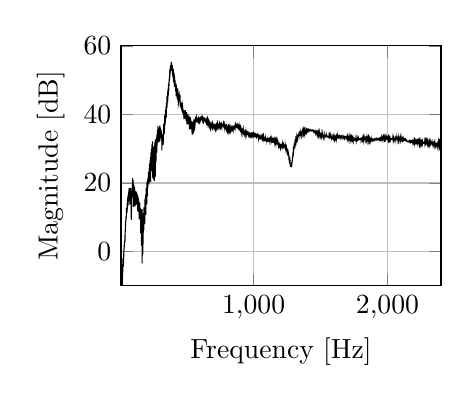
\begin{tikzpicture}

\begin{axis}[%
width=1.6in,
height=1.2in,
at={(1.011in,0.642in)},
scale only axis,
xmin=10,
xmax=2400,
xmajorgrids,
ymin=-10,
ymax=60,
ymajorgrids,
ylabel={Magnitude [dB]},
xlabel={Frequency [Hz]},
axis background/.style={fill=white}
]
\addplot [color=black,solid,forget plot]
  table[row sep=crcr]{%
0	-16.4207408876761\\
0.666675926054529	-16.3154176276792\\
1.33335185210906	-14.3774180210266\\
2.00002777816359	-6.86555584658154\\
2.66670370421811	-11.3465042481908\\
3.33337963027264	-3.34374464204505\\
4.00005555632717	-7.11107109532166\\
4.6667314823817	-12.1693667358472\\
5.33340740843623	-0.119216488529928\\
6.00008333449076	-2.4063735260876\\
6.66675926054529	-3.84005871388903\\
7.33343518659981	-4.09285612918779\\
8.00011111265434	-23.0585301953459\\
8.66678703870887	-9.33441526588072\\
9.3334629647634	-14.2451665128663\\
10.0001388908179	-14.8936015760657\\
10.6668148168725	-11.4025566251672\\
11.333490742927	-15.9060191722353\\
12.0001666689815	-17.9060905497264\\
12.666842595036	-21.3086681740886\\
13.3335185210906	-15.2428005028356\\
14.0001944471451	-15.876909830105\\
14.6668703731996	-28.3976100362418\\
15.3335462992542	-11.0618700517958\\
16.0002222253087	-11.8670029139117\\
16.6668981513632	-16.3171543397441\\
17.3335740774177	-20.6379340561335\\
18.0002500034723	-9.31206157628221\\
18.6669259295268	-4.31219018330604\\
19.3336018555813	-7.75611333089071\\
20.0002777816359	-10.0273871967221\\
20.6669537076904	-7.46000207181059\\
21.3336296337449	-6.27033798836338\\
22.0003055597994	-5.54088897246489\\
22.666981485854	-5.87482356201717\\
23.3336574119085	-3.55246459447764\\
24.000333337963	-3.40076605840831\\
24.6670092640176	-2.8403814904178\\
25.3336851900721	-1.89749689474223\\
26.0003611161266	-2.45706549259375\\
26.6670370421811	-4.40691738201516\\
27.3337129682357	-3.96314171765353\\
28.0003888942902	-3.19805021717539\\
28.6670648203447	-3.18059986733467\\
29.3337407463993	-2.81074645132835\\
30.0004166724538	-1.53901268372035\\
30.6670925985083	-0.551761435037259\\
31.3337685245628	0.533219314324133\\
32.0004444506174	0.305706428293476\\
32.6671203766719	0.831588978237437\\
33.3337963027264	0.923161804473851\\
34.000472228781	1.49850174143959\\
34.6671481548355	1.66389384465929\\
35.33382408089	2.12726491351963\\
36.0005000069445	2.82948710203715\\
36.6671759329991	2.47689360231122\\
37.3338518590536	3.05972493193646\\
38.0005277851081	2.72469832813045\\
38.6672037111627	3.20770904266964\\
39.3338796372172	3.01722752485322\\
40.0005555632717	4.7069642154083\\
40.6672314893262	5.41090854302455\\
41.3339074153808	5.72676114726331\\
42.0005833414353	6.28375290096039\\
42.6672592674898	6.73923267959653\\
43.3339351935444	7.39831616402118\\
44.0006111195989	8.43513597838629\\
44.6672870456534	8.39612545299579\\
45.3339629717079	8.91565851232458\\
46.0006388977625	9.0041296508419\\
46.667314823817	9.27177569981162\\
47.3339907498715	9.95654351075711\\
48.0006666759261	9.46248251453852\\
48.6673426019806	9.95330724986174\\
49.3340185280351	9.97961690593952\\
50.0006944540896	12.6850341034311\\
50.6673703801442	10.9898208225939\\
51.3340463061987	11.4367121280973\\
52.0007222322532	12.250889982447\\
52.6673981583078	11.5501187749667\\
53.3340740843623	11.7072195297964\\
54.0007500104168	12.8409009817643\\
54.6674259364713	12.6816331787994\\
55.3341018625259	11.3412101217346\\
56.0007777885804	13.5420485162717\\
56.6674537146349	14.0784290449487\\
57.3341296406895	12.4453825383\\
58.000805566744	14.0107760690413\\
58.6674814927985	15.1479898993026\\
59.334157418853	13.4431365825266\\
60.0008333449076	14.4881850219695\\
60.6675092709621	15.5759786271557\\
61.3341851970166	14.5720950310454\\
62.0008611230712	15.6696742092471\\
62.6675370491257	16.342397721758\\
63.3342129751802	13.4098839750679\\
64.0008889012347	16.2262267765787\\
64.6675648272893	15.8411530418611\\
65.3342407533438	14.4771936155389\\
66.0009166793983	16.7473404674684\\
66.6675926054529	14.8347985258206\\
67.3342685315074	17.4094530943439\\
68.0009444575619	17.0411502715459\\
68.6676203836164	15.8107772154615\\
69.334296309671	18.0127106973106\\
70.0009722357255	16.6685205126036\\
70.66764816178	16.9189658025146\\
71.3343240878346	18.5563486025286\\
72.0010000138891	15.8117840802981\\
72.6676759399436	17.3971487845641\\
73.3343518659981	16.813819435762\\
74.0010277920527	16.4624730963978\\
74.6677037181072	16.2270054080207\\
75.3343796441617	16.2741635363144\\
76.0010555702163	18.0626837102414\\
76.6677314962708	13.7079761110671\\
77.3344074223253	16.2671366430792\\
78.0010833483798	16.7132237489781\\
78.6677592744344	14.508981776001\\
79.3344352004889	18.0860020681766\\
80.0011111265434	16.1555220764925\\
80.667787052598	17.5761027428361\\
81.3344629786525	16.3797234021374\\
82.001138904707	18.52346807256\\
82.6678148307615	16.0573716852031\\
83.3344907568161	16.1701923023411\\
84.0011666828706	15.1472176768799\\
84.6678426089251	13.6999659886751\\
85.3345185349797	13.9542755547642\\
86.0011944610342	9.72792294202415\\
86.6678703870887	11.3996372527738\\
87.3345463131432	9.26118427135271\\
88.0012222391978	12.3064431901164\\
88.6678981652523	11.5211265689239\\
89.3345740913068	15.43044499846\\
90.0012500173614	15.5947669591699\\
90.6679259434159	17.6406520063406\\
91.3346018694704	17.4770285388202\\
92.0012777955249	17.6100445670831\\
92.6679537215795	16.8975238085485\\
93.334629647634	17.4299533217051\\
94.0013055736885	18.62735118896\\
94.667981499743	17.4942372510506\\
95.3346574257976	20.7916657131854\\
96.0013333518521	18.2774536883704\\
96.6680092779066	21.3769284932748\\
97.3346852039612	18.5485066206733\\
98.0013611300157	20.3569008716082\\
98.6680370560702	18.1977081417711\\
99.3347129821248	20.7993685463794\\
100.001388908179	19.1333198158665\\
100.668064834234	18.8434548014757\\
101.334740760288	19.8213343203061\\
102.001416686343	12.9886025710954\\
102.668092612397	18.7795686658998\\
103.334768538452	16.5223787347286\\
104.001444464506	16.0379885502662\\
104.668120390561	17.6124305559709\\
105.334796316616	15.8038793338395\\
106.00147224267	19.4162917879813\\
106.668148168725	16.5327627463201\\
107.334824094779	17.8444951421687\\
108.001500020834	17.890320298304\\
108.668175946888	14.5910187828617\\
109.334851872943	17.0001588871409\\
110.001527798997	15.4502531397764\\
110.668203725052	16.5402249086946\\
111.334879651106	18.8726363694092\\
112.001555577161	13.1792573163142\\
112.668231503215	15.8598047731048\\
113.33490742927	17.462462953448\\
114.001583355324	14.7374983698052\\
114.668259281379	14.6172049678678\\
115.334935207433	17.2313216471\\
116.001611133488	14.9160434571698\\
116.668287059542	15.754877493657\\
117.334962985597	15.2663676769536\\
118.001638911652	14.6220739984028\\
118.668314837706	17.1952846169961\\
119.334990763761	17.134539026807\\
120.001666689815	14.2387030019275\\
120.66834261587	15.6734788729892\\
121.335018541924	15.7872007302215\\
122.001694467979	14.1193035314621\\
122.668370394033	15.7441197766407\\
123.335046320088	17.4400855143237\\
124.001722246142	14.9400729709756\\
124.668398172197	13.6977564605611\\
125.335074098251	15.4262942897941\\
126.001750024306	15.9544054196553\\
126.66842595036	14.2970436756401\\
127.335101876415	15.5519693706824\\
128.001777802469	16.3392824814393\\
128.668453728524	15.3036892209872\\
129.335129654579	13.9176814548077\\
130.001805580633	14.7429683751012\\
130.668481506688	14.4989917516002\\
131.335157432742	15.0472882360648\\
132.001833358797	16.2453331527152\\
132.668509284851	16.2991525070823\\
133.335185210906	15.5300469108267\\
134.00186113696	12.8727962850214\\
134.668537063015	12.6515530322373\\
135.335212989069	11.911385204764\\
136.001888915124	13.8169664447145\\
136.668564841178	12.5408705093649\\
137.335240767233	13.2018319904848\\
138.001916693287	12.791900107419\\
138.668592619342	11.4917353551962\\
139.335268545396	13.8010576485913\\
140.001944471451	13.6393101017531\\
140.668620397506	14.2704220930981\\
141.33529632356	14.4743956933171\\
142.001972249615	14.1606974105989\\
142.668648175669	14.6566417574254\\
143.335324101724	13.0228798879614\\
144.002000027778	12.8211006139036\\
144.668675953833	11.7343846134064\\
145.335351879887	9.48036552928666\\
146.002027805942	11.4702366388333\\
146.668703731996	9.36705943560544\\
147.335379658051	10.5399431599512\\
148.002055584105	10.5853488286803\\
148.66873151016	11.5759601359361\\
149.335407436214	12.9665410909005\\
150.002083362269	14.2738294429082\\
150.668759288323	13.0066856156558\\
151.335435214378	12.3196979809724\\
152.002111140433	10.3437099049964\\
152.668787066487	11.1975695329164\\
153.335462992542	12.2000623926555\\
154.002138918596	12.4614010073805\\
154.668814844651	12.4643406565909\\
155.335490770705	10.6924706114413\\
156.00216669676	9.68384261497514\\
156.668842622814	8.35277518877358\\
157.335518548869	5.38115419806178\\
158.002194474923	7.90129966020449\\
158.668870400978	6.99051579707439\\
159.335546327032	7.19230262657555\\
160.002222253087	12.2234245677309\\
160.668898179141	11.4304876801609\\
161.335574105196	6.57268371176491\\
162.00225003125	10.7867440200595\\
162.668925957305	7.92297843305203\\
163.335601883359	1.72857143932076\\
164.002277809414	5.55842036054592\\
164.668953735469	9.53301079418227\\
165.335629661523	7.97117577823556\\
166.002305587578	9.8205785154508\\
166.668981513632	12.3509079222075\\
167.335657439687	8.80481170070022\\
168.002333365741	-3.43251842784511\\
168.669009291796	7.99961874303782\\
169.33568521785	10.9285078575774\\
170.002361143905	9.47874609405068\\
170.669037069959	6.14794665007641\\
171.335712996014	10.2393266984326\\
172.002388922068	6.58206895352054\\
172.669064848123	-0.794404927034236\\
173.335740774177	9.71375690335453\\
174.002416700232	11.1208918798069\\
174.669092626286	6.33091683985413\\
175.335768552341	2.18321304534534\\
176.002444478396	10.999493518594\\
176.66912040445	10.4234872073946\\
177.335796330505	5.99082217749483\\
178.002472256559	7.13775234873263\\
178.669148182614	11.21849572383\\
179.335824108668	10.4278246364209\\
180.002500034723	6.29007280326203\\
180.669175960777	10.2619608566445\\
181.335851886832	12.0189956450697\\
182.002527812886	12.8681982819018\\
182.669203738941	7.89861206701179\\
183.335879664995	8.85333509911726\\
184.00255559105	12.1287707105828\\
184.669231517104	11.1683680196191\\
185.335907443159	11.262724032992\\
186.002583369213	12.4485107147759\\
186.669259295268	11.0900180161446\\
187.335935221323	8.12095971430723\\
188.002611147377	11.7415510241294\\
188.669287073432	15.2016108361629\\
189.335962999486	13.4221058252019\\
190.002638925541	13.9609298125596\\
190.669314851595	12.4379269995488\\
191.33599077765	15.038267283522\\
192.002666703704	15.6609417012862\\
192.669342629759	14.2281810127311\\
193.336018555813	16.5079745434322\\
194.002694481868	13.902769900181\\
194.669370407922	10.6764455289808\\
195.336046333977	13.8125291233786\\
196.002722260031	13.5743392461096\\
196.669398186086	14.7919309286161\\
197.33607411214	16.356292659487\\
198.002750038195	18.5636270251696\\
198.66942596425	17.9099527777734\\
199.336101890304	16.9980432961722\\
200.002777816359	16.0616184931362\\
200.669453742413	15.2700660608917\\
201.336129668468	13.7563910232203\\
202.002805594522	17.8947583995335\\
202.669481520577	14.0524167208802\\
203.336157446631	20.1418512122755\\
204.002833372686	18.2094666492722\\
204.66950929874	18.2162066807638\\
205.336185224795	18.452256391217\\
206.002861150849	16.1740249613505\\
206.669537076904	18.4593995883224\\
207.336213002958	18.8062215348524\\
208.002888929013	20.5598410737591\\
208.669564855067	20.6804089526863\\
209.336240781122	19.7016726547674\\
210.002916707176	19.3924393136311\\
210.669592633231	19.3209208451602\\
211.336268559286	19.9173874750075\\
212.00294448534	21.6051521212416\\
212.669620411395	21.0926629267911\\
213.336296337449	19.7776153799872\\
214.002972263504	20.9087654796494\\
214.669648189558	21.6402946716591\\
215.336324115613	23.1660904969058\\
216.003000041667	22.2647379205029\\
216.669675967722	20.7986772241991\\
217.336351893776	19.6086407951983\\
218.003027819831	21.7864878798544\\
218.669703745885	22.7132328825598\\
219.33637967194	21.836530120458\\
220.003055597994	20.0301674171574\\
220.669731524049	20.6902390179615\\
221.336407450103	25.2287777090685\\
222.003083376158	23.8844050316427\\
222.669759302213	23.6702456707145\\
223.336435228267	22.197732392584\\
224.003111154322	25.1858546090586\\
224.669787080376	25.7286333362144\\
225.336463006431	22.7809142705303\\
226.003138932485	23.0307277556132\\
226.66981485854	24.2895189233463\\
227.336490784594	26.6885996899686\\
228.003166710649	22.2340200064072\\
228.669842636703	21.2042591407827\\
229.336518562758	27.4448491378671\\
230.003194488812	24.998464787914\\
230.669870414867	20.2844894992543\\
231.336546340921	26.229295173424\\
232.003222266976	27.3704729407457\\
232.66989819303	24.235163800278\\
233.336574119085	23.6365252132475\\
234.00325004514	28.8218793911986\\
234.669925971194	26.4501209493808\\
235.336601897249	23.359698189082\\
236.003277823303	29.0942573930333\\
236.669953749358	28.888242504493\\
237.336629675412	23.6588037647213\\
238.003305601467	29.5222764152547\\
238.669981527521	29.9822130112762\\
239.336657453576	24.4960469956987\\
240.00333337963	29.6706196201175\\
240.670009305685	31.2099832894061\\
241.336685231739	23.5871051356198\\
242.003361157794	30.628374330598\\
242.670037083848	30.6223139233049\\
243.336713009903	24.4159715317574\\
244.003388935957	31.8246031729028\\
244.670064862012	28.8034864020243\\
245.336740788066	27.0157090140757\\
246.003416714121	32.1041911580651\\
246.670092640176	21.657366174581\\
247.33676856623	30.0261274627137\\
248.003444492285	29.3882025514685\\
248.670120418339	23.6369360028534\\
249.336796344394	30.594362746759\\
250.003472270448	21.0864166816281\\
250.670148196503	28.1448227968013\\
251.336824122557	27.5609770479509\\
252.003500048612	24.3135415395441\\
252.670175974666	29.9105522897886\\
253.336851900721	22.8890707062304\\
254.003527826775	29.1623191496647\\
254.67020375283	27.3158979888956\\
255.336879678884	26.4977460092467\\
256.003555604939	29.9536038840458\\
256.670231530993	21.9438846229577\\
257.336907457048	30.5050174370217\\
258.003583383103	20.5857661865682\\
258.670259309157	29.5903277763299\\
259.336935235212	25.7160396637146\\
260.003611161266	28.7467800415489\\
260.670287087321	29.161184746739\\
261.336963013375	29.0325576777374\\
262.00363893943	31.2009778266953\\
262.670314865484	26.5870809538211\\
263.336990791539	31.9980110688954\\
264.003666717593	21.7674712020672\\
264.670342643648	31.6185778808993\\
265.337018569702	21.9654617689814\\
266.003694495757	30.8458692652959\\
266.670370421811	23.974169355403\\
267.337046347866	32.5001492095142\\
268.00372227392	26.5434817430343\\
268.670398199975	32.6049413877319\\
269.33707412603	27.7400128261142\\
270.003750052084	32.4964750930296\\
270.670425978139	25.9385550539772\\
271.337101904193	32.7387060088865\\
272.003777830248	26.5299755364714\\
272.670453756302	32.2508610107737\\
273.337129682357	29.8257861467402\\
274.003805608411	33.246733960407\\
274.670481534466	30.3789975832668\\
275.33715746052	31.3449998215966\\
276.003833386575	30.7953803666772\\
276.670509312629	28.865777157565\\
277.337185238684	32.9322191750248\\
278.003861164738	30.114184585594\\
278.670537090793	34.0666160933313\\
279.337213016847	30.8426561684383\\
280.003888942902	31.2550390631154\\
280.670564868956	33.2247884113133\\
281.337240795011	32.1486105650566\\
282.003916721066	35.3894272189679\\
282.67059264712	31.7462682285058\\
283.337268573175	33.2199117531558\\
284.003944499229	34.2916327319487\\
284.670620425284	32.6106234428527\\
285.337296351338	36.5466486400287\\
286.003972277393	33.7019400282432\\
286.670648203447	33.0998900770943\\
287.337324129502	34.6389581442847\\
288.004000055556	33.4211815136646\\
288.670675981611	35.666899519188\\
289.337351907665	35.1708956768408\\
290.00402783372	31.8251905305127\\
290.670703759774	33.8179261233312\\
291.337379685829	35.705461240345\\
292.004055611883	34.9151897399752\\
292.670731537938	33.6630291547895\\
293.337407463993	33.5050006037983\\
294.004083390047	34.396603973026\\
294.670759316102	35.4126024257686\\
295.337435242156	36.1524348865116\\
296.004111168211	34.3797980645959\\
296.670787094265	32.090658390672\\
297.33746302032	35.3052512738886\\
298.004138946374	36.443293502769\\
298.670814872429	33.0284838187466\\
299.337490798483	33.3737636569273\\
300.004166724538	36.8172751045972\\
300.670842650592	36.2536354732602\\
301.337518576647	33.5084746600786\\
302.004194502701	34.3107511055723\\
302.670870428756	36.0872095107185\\
303.33754635481	34.8930926380767\\
304.004222280865	33.1713466810146\\
304.67089820692	34.3963284340929\\
305.337574132974	36.0954048526824\\
306.004250059029	35.8623758681692\\
306.670925985083	34.9394782240887\\
307.337601911138	35.4933626834169\\
308.004277837192	34.6998396602613\\
308.670953763247	33.9886274539985\\
309.337629689301	35.4487032195695\\
310.004305615356	34.9790323278319\\
310.67098154141	32.2959058344289\\
311.337657467465	32.5470597503387\\
312.004333393519	34.1686009341095\\
312.671009319574	32.3101951319522\\
313.337685245628	32.5546308203229\\
314.004361171683	34.2994418113994\\
314.671037097737	32.9638261635451\\
315.337713023792	29.5246581143845\\
316.004388949847	32.1962891792166\\
316.671064875901	32.6597274745189\\
317.337740801956	30.8340415383325\\
318.00441672801	33.3220678967992\\
318.671092654065	33.7618842351523\\
319.337768580119	31.8337953547213\\
320.004444506174	34.1572329959546\\
320.671120432228	32.3020964554841\\
321.337796358283	31.3440734995687\\
322.004472284337	32.5402223824718\\
322.671148210392	32.3228555367296\\
323.337824136446	31.3206184268438\\
324.004500062501	33.0824041651311\\
324.671175988555	31.1035899774478\\
325.33785191461	32.3154650463354\\
326.004527840664	34.2088402467855\\
326.671203766719	34.0773848396265\\
327.337879692774	35.2554090957086\\
328.004555618828	35.9988544467471\\
328.671231544883	34.8923579484064\\
329.337907470937	37.2770903151213\\
330.004583396992	37.054475790932\\
330.671259323046	37.0091870723092\\
331.337935249101	37.2975116167771\\
332.004611175155	35.9472167531336\\
332.67128710121	35.5700950062361\\
333.337963027264	35.6769573425815\\
334.004638953319	34.2542600873256\\
334.671314879373	37.1105094082618\\
335.337990805428	36.8853319468742\\
336.004666731482	39.6816057295463\\
336.671342657537	38.7322650834837\\
337.338018583591	38.6252441254422\\
338.004694509646	38.8458438971479\\
338.671370435701	36.9234118006859\\
339.338046361755	38.0527831040288\\
340.00472228781	37.5640908745272\\
340.671398213864	39.9016898613973\\
341.338074139919	41.2514904378187\\
342.004750065973	39.761310032034\\
342.671425992028	41.2450171108603\\
343.338101918082	38.651984842571\\
344.004777844137	38.9809937449846\\
344.671453770191	39.1032274346479\\
345.338129696246	41.64049740428\\
346.0048056223	42.1470224520002\\
346.671481548355	40.717768695391\\
347.338157474409	41.2063227288448\\
348.004833400464	39.1701740844293\\
348.671509326518	42.7153329266851\\
349.338185252573	42.5040048526065\\
350.004861178627	43.3783005460081\\
350.671537104682	41.6581998577334\\
351.338213030737	42.5484522235291\\
352.004888956791	42.3459886976922\\
352.671564882846	45.1690954725839\\
353.3382408089	43.8881999562138\\
354.004916734955	42.0205363419269\\
354.671592661009	43.1504332274118\\
355.338268587064	45.4538334962571\\
356.004944513118	44.7011145843496\\
356.671620439173	43.4830870101132\\
357.338296365227	43.4896280170572\\
358.004972291282	45.9581345895163\\
358.671648217336	46.5891561118104\\
359.338324143391	44.1528542519465\\
360.005000069445	44.9742415835098\\
360.6716759955	46.8377429327789\\
361.338351921554	46.8238968362695\\
362.005027847609	45.2851211482967\\
362.671703773664	45.978913865933\\
363.338379699718	48.498325482995\\
364.005055625773	46.7979377558064\\
364.671731551827	47.3219044770167\\
365.338407477882	46.8364891373161\\
366.005083403936	48.9002884827329\\
366.671759329991	46.9567945256404\\
367.338435256045	49.5500807672716\\
368.0051111821	48.334699559823\\
368.671787108154	48.6213370004008\\
369.338463034209	49.2244008451691\\
370.005138960263	50.3608735458051\\
370.671814886318	49.6887875019567\\
371.338490812372	49.9910400450476\\
372.005166738427	51.3654018269137\\
372.671842664481	49.9133019483712\\
373.338518590536	52.6732587462788\\
374.005194516591	50.6970466620926\\
374.671870442645	52.8824120149749\\
375.3385463687	51.6078573426022\\
376.005222294754	53.1822094446027\\
376.671898220809	52.3134742014947\\
377.338574146863	53.5171376882159\\
378.005250072918	53.1408821134094\\
378.671925998972	53.2074241342539\\
379.338601925027	53.7350363329004\\
380.005277851081	54.0910710317313\\
380.671953777136	54.0730656126014\\
381.33862970319	54.1206378717553\\
382.005305629245	53.4816743666175\\
382.671981555299	54.110831727205\\
383.338657481354	53.9098043201159\\
384.005333407408	52.9923167378291\\
384.672009333463	55.0572254303735\\
385.338685259517	52.6363635255162\\
386.005361185572	55.3222144845658\\
386.672037111627	53.1278013347387\\
387.338713037681	53.4105859410106\\
388.005388963736	55.0759537627728\\
388.67206488979	52.6697713413235\\
389.338740815845	54.5297276084042\\
390.005416741899	54.1984179541779\\
390.672092667954	52.59919558716\\
391.338768594008	53.9663054007644\\
392.005444520063	52.9254502822928\\
392.672120446117	52.8557226602076\\
393.338796372172	54.3073252192827\\
394.005472298226	51.6053529564713\\
394.672148224281	52.5469919607313\\
395.338824150335	53.4922505512102\\
396.00550007639	51.286402887989\\
396.672176002444	53.1532065570996\\
397.338851928499	52.493531315183\\
398.005527854554	50.9928722677272\\
398.672203780608	52.5685335946956\\
399.338879706663	52.9896841245112\\
400.005555632717	50.7603680832008\\
400.672231558772	51.4288645476436\\
401.338907484826	53.2359628819213\\
402.005583410881	49.8374227604454\\
402.672259336935	51.4467697765609\\
403.33893526299	51.9414891214234\\
404.005611189044	49.4149498988904\\
404.672287115099	50.1202375353717\\
405.338963041153	51.9999054104195\\
406.005638967208	50.4953516728399\\
406.672314893262	48.9901599276187\\
407.338990819317	50.158647636806\\
408.005666745371	51.3920831088233\\
408.672342671426	49.5431285314291\\
409.339018597481	48.08256015592\\
410.005694523535	50.8775920612461\\
410.67237044959	50.3229934576393\\
411.339046375644	48.0085417213772\\
412.005722301699	48.529719009823\\
412.672398227753	49.9855174586646\\
413.339074153808	48.8396320469932\\
414.005750079862	48.06851030515\\
414.672426005917	48.5405236843253\\
415.339101931971	48.8861738889943\\
416.005777858026	48.0896469929758\\
416.67245378408	48.7425822245499\\
417.339129710135	48.0541022602256\\
418.005805636189	47.4714618584139\\
418.672481562244	46.825388597866\\
419.339157488298	47.8640749027073\\
420.005833414353	49.0125888840837\\
420.672509340407	47.725978896795\\
421.339185266462	45.2547215464681\\
422.005861192517	46.637294648805\\
422.672537118571	48.1949618032884\\
423.339213044626	48.4193750100493\\
424.00588897068	47.4383063333612\\
424.672564896735	45.9150112175033\\
425.339240822789	46.1249928196961\\
426.005916748844	46.7156849446243\\
426.672592674898	46.695820592414\\
427.339268600953	46.8121412489869\\
428.005944527007	46.7915091529435\\
428.672620453062	47.2380291543304\\
429.339296379116	47.1566144657491\\
430.005972305171	45.5230909590603\\
430.672648231225	44.2901522108859\\
431.33932415728	44.6657521431216\\
432.006000083334	45.9259706546435\\
432.672676009389	47.0066861675098\\
433.339351935444	47.0645967555485\\
434.006027861498	45.7014576723324\\
434.672703787553	45.6514042661947\\
435.339379713607	46.2041099163959\\
436.006055639662	45.5498132755874\\
436.672731565716	45.1873747573363\\
437.339407491771	44.3770788651156\\
438.006083417825	43.0712652110201\\
438.67275934388	43.2094964401877\\
439.339435269934	43.8498842499073\\
440.006111195989	45.0238296465671\\
440.672787122043	45.0698160723354\\
441.339463048098	44.2306680597435\\
442.006138974152	44.1174690364718\\
442.672814900207	44.2259883579088\\
443.339490826261	45.2522883425857\\
444.006166752316	45.6863850714493\\
444.672842678371	45.8313410861746\\
445.339518604425	45.6024701251868\\
446.00619453048	45.1887499819467\\
446.672870456534	44.5126571011511\\
447.339546382589	44.1204579951574\\
448.006222308643	43.7747266426837\\
448.672898234698	44.3016666920141\\
449.339574160752	44.9575828597661\\
450.006250086807	45.5719474682794\\
450.672926012861	45.2629398911049\\
451.339601938916	44.4267090654131\\
452.00627786497	43.4211042206743\\
452.672953791025	42.7337558511264\\
453.339629717079	42.8327649387839\\
454.006305643134	42.9235618784751\\
454.672981569188	43.3139660992203\\
455.339657495243	43.2329805899851\\
456.006333421298	43.0875773890865\\
456.673009347352	42.2331765899717\\
457.339685273407	42.4533398711911\\
458.006361199461	43.0113096961461\\
458.673037125516	42.8257817316036\\
459.33971305157	42.7161739036484\\
460.006388977625	42.4899561041258\\
460.673064903679	42.2805348450519\\
461.339740829734	42.5900480042906\\
462.006416755788	42.6518318473933\\
462.673092681843	42.3209667883899\\
463.339768607897	41.8722742726514\\
464.006444533952	41.7199219161373\\
464.673120460006	43.1283461820559\\
465.339796386061	43.2242704480207\\
466.006472312115	42.7728226913247\\
466.67314823817	43.4447342128753\\
467.339824164225	42.8250951804206\\
468.006500090279	42.4692779668213\\
468.673176016334	41.7097857991288\\
469.339851942388	41.3973327680734\\
470.006527868443	42.6258976868372\\
470.673203794497	41.7657072108801\\
471.339879720552	40.4917754996181\\
472.006555646606	41.2384315145316\\
472.673231572661	40.8042554486369\\
473.339907498715	40.138441711244\\
474.00658342477	40.9827437802688\\
474.673259350824	41.3313928866248\\
475.339935276879	40.2988431521779\\
476.006611202933	40.0207620168218\\
476.673287128988	41.0190558098767\\
477.339963055042	39.9025700525159\\
478.006638981097	39.7832762468912\\
478.673314907152	41.1158707558027\\
479.339990833206	39.7456161348829\\
480.006666759261	39.8461631773169\\
480.673342685315	40.2709311883775\\
481.34001861137	39.4320285031454\\
482.006694537424	40.1565909562264\\
482.673370463479	40.1811282949547\\
483.340046389533	38.7372107954452\\
484.006722315588	40.8530372817629\\
484.673398241642	40.1875887039174\\
485.340074167697	39.1390724327409\\
486.006750093751	40.9987184719945\\
486.673426019806	40.1423689750495\\
487.34010194586	40.821905030225\\
488.006777871915	40.2711170031615\\
488.673453797969	40.9106946388373\\
489.340129724024	41.2281751872643\\
490.006805650078	38.7539058797657\\
490.673481576133	41.1581563766563\\
491.340157502188	40.1422509255701\\
492.006833428242	39.7188355439635\\
492.673509354297	40.1178368706808\\
493.340185280351	38.7653827264783\\
494.006861206406	40.0215673334073\\
494.67353713246	38.8197796349121\\
495.340213058515	38.7638869261884\\
496.006888984569	38.4527061709988\\
496.673564910624	39.6501640282925\\
497.340240836678	38.0347061243894\\
498.006916762733	40.6115595124091\\
498.673592688787	38.3732507989096\\
499.340268614842	40.6230771315451\\
500.006944540896	39.5349707839303\\
500.673620466951	39.7061509066729\\
501.340296393005	39.6484917363652\\
502.00697231906	38.1058958707444\\
502.673648245115	38.2126966811948\\
503.340324171169	37.8003348858246\\
504.007000097224	38.5353936247167\\
504.673676023278	38.7925117504884\\
505.340351949333	38.6922010453484\\
506.007027875387	40.1784575379699\\
506.673703801442	38.139688169341\\
507.340379727496	39.5412614385339\\
508.007055653551	37.0696904106757\\
508.673731579605	39.3687772515517\\
509.34040750566	37.2641971190393\\
510.007083431714	39.3335875949048\\
510.673759357769	38.9945022712591\\
511.340435283823	39.0434479076378\\
512.007111209878	39.3977665930757\\
512.673787135932	37.1341742663097\\
513.340463061987	38.4678879111901\\
514.007138988041	37.1215248994681\\
514.673814914096	38.8754468674613\\
515.340490840151	38.8155902487941\\
516.007166766205	38.9643961413851\\
516.67384269226	38.6207255538515\\
517.340518618314	37.3357735428765\\
518.007194544369	37.0666323909037\\
518.673870470423	38.7211223841895\\
519.340546396478	37.2512036749153\\
520.007222322532	38.8378789455878\\
520.673898248587	39.0540454949482\\
521.340574174641	35.6167194973003\\
522.007250100696	38.5805907798575\\
522.67392602675	37.9716781075863\\
523.340601952805	38.0567765453894\\
524.007277878859	38.9474356140497\\
524.673953804914	35.6144584944386\\
525.340629730968	36.9567239164733\\
526.007305657023	39.3381037143048\\
526.673981583078	37.0163501594176\\
527.340657509132	37.954178080984\\
528.007333435187	37.8363684385321\\
528.674009361241	36.2982367441304\\
529.340685287296	37.2471296218255\\
530.00736121335	38.8768972606465\\
530.674037139405	36.529967710998\\
531.340713065459	35.7238922476624\\
532.007388991514	37.4490725441219\\
532.674064917568	38.0734512069854\\
533.340740843623	36.9632879442554\\
534.007416769677	36.0249547505336\\
534.674092695732	37.141953529701\\
535.340768621786	38.1045780990821\\
536.007444547841	36.6073979552001\\
536.674120473896	35.810551186352\\
537.34079639995	36.8765322890455\\
538.007472326005	37.4354479890167\\
538.674148252059	35.8182884787281\\
539.340824178114	34.9363622286156\\
540.007500104168	36.6500701363602\\
540.674176030223	37.9050253824154\\
541.340851956277	36.0659766282051\\
542.007527882332	34.0872106818742\\
542.674203808386	35.1318828237975\\
543.340879734441	37.1969220998263\\
544.007555660495	36.605128199528\\
544.67423158655	34.3390094827634\\
545.340907512604	35.8172589824666\\
546.007583438659	36.7194665646319\\
546.674259364713	36.0171662084705\\
547.340935290768	37.0597282417885\\
548.007611216823	37.1736144343115\\
548.674287142877	35.2046714031081\\
549.340963068932	34.477484254241\\
550.007638994986	36.2229785012706\\
550.674314921041	36.2894021152438\\
551.340990847095	36.3196840268027\\
552.00766677315	36.5205133524459\\
552.674342699204	36.5785236380741\\
553.341018625259	34.7941344325039\\
554.007694551313	35.3480029949818\\
554.674370477368	36.363631366636\\
555.341046403422	35.8022507922789\\
556.007722329477	36.9036641788603\\
556.674398255531	38.2712850941599\\
557.341074181586	36.7336546477984\\
558.00775010764	37.5899753149851\\
558.674426033695	37.4875857539739\\
559.341101959749	36.5184117796704\\
560.007777885804	36.3935217137143\\
560.674453811858	36.8382351102893\\
561.341129737913	36.1741575481076\\
562.007805663968	36.9062111206471\\
562.674481590022	37.759130065319\\
563.341157516077	36.9076262331354\\
564.007833442131	38.1503397567839\\
564.674509368186	38.1044083112786\\
565.34118529424	37.6143624038454\\
566.007861220295	39.0836888745263\\
566.674537146349	38.5984076611432\\
567.341213072404	39.0349668401718\\
568.007888998458	39.3462004112958\\
568.674564924513	38.3858183700981\\
569.341240850567	38.4554476353851\\
570.007916776622	38.3187131280869\\
570.674592702676	37.7096564944676\\
571.341268628731	38.7909536850105\\
572.007944554785	37.9958435199494\\
572.67462048084	38.4805326124803\\
573.341296406895	38.8039959579789\\
574.007972332949	38.6047617007948\\
574.674648259004	39.1841261260577\\
575.341324185058	38.4181976272362\\
576.008000111113	37.8862451937344\\
576.674676037167	38.0998718042378\\
577.341351963222	37.6984656665166\\
578.008027889276	38.7385819158181\\
578.674703815331	38.4193106969419\\
579.341379741385	38.767588689429\\
580.00805566744	38.4660786172894\\
580.674731593494	37.991506008421\\
581.341407519549	38.4205984026107\\
582.008083445603	37.8798585699589\\
582.674759371658	39.0059117128521\\
583.341435297712	38.2472238281507\\
584.008111223767	38.1114308617772\\
584.674787149822	37.6839988146084\\
585.341463075876	38.5133189005044\\
586.008139001931	38.8775712475661\\
586.674814927985	38.3683193076294\\
587.34149085404	38.7521184065546\\
588.008166780094	37.5526856533378\\
588.674842706149	38.415784984347\\
589.341518632203	38.4680338504117\\
590.008194558258	39.0198613920213\\
590.674870484312	37.3414027331125\\
591.341546410367	38.5206621797882\\
592.008222336421	38.4136028816329\\
592.674898262476	38.3174888877935\\
593.34157418853	37.9300403990023\\
594.008250114585	38.7556041082405\\
594.674926040639	38.1667066384737\\
595.341601966694	38.212727045325\\
596.008277892749	38.102660901164\\
596.674953818803	38.6390298030887\\
597.341629744858	38.5893821977963\\
598.008305670912	38.1639016836855\\
598.674981596967	38.0980346419261\\
599.341657523021	39.1101818730067\\
600.008333449076	38.0670266839222\\
600.67500937513	38.0665522129434\\
601.341685301185	38.6187015436325\\
602.008361227239	38.8584999066903\\
602.675037153294	37.9240098873232\\
603.341713079348	39.000321049987\\
604.008389005403	38.4191745533299\\
604.675064931457	39.0058247555154\\
605.341740857512	38.1887826281489\\
606.008416783566	39.1937013947967\\
606.675092709621	38.1469952487889\\
607.341768635676	39.4276942168322\\
608.00844456173	38.2589822266757\\
608.675120487785	39.0133688655693\\
609.341796413839	38.9783915200063\\
610.008472339894	38.3804936224\\
610.675148265948	39.3208230747345\\
611.341824192003	38.2806005275172\\
612.008500118057	38.8796896190854\\
612.675176044112	38.6531572409538\\
613.341851970166	38.9558248400456\\
614.008527896221	38.5991210004159\\
614.675203822275	39.1988923816612\\
615.34187974833	38.564628107045\\
616.008555674384	39.0185061177037\\
616.675231600439	38.8535743043408\\
617.341907526493	38.7069279545918\\
618.008583452548	39.0455299272677\\
618.675259378603	38.5718214238489\\
619.341935304657	38.9042605032751\\
620.008611230711	38.8588149643079\\
620.675287156766	38.5023025912238\\
621.341963082821	38.7102224611168\\
622.008639008875	38.6124297978375\\
622.67531493493	38.4968940494402\\
623.341990860984	39.1667865213447\\
624.008666787039	38.0776452264106\\
624.675342713093	39.1639161221302\\
625.342018639148	38.4145315375555\\
626.008694565202	38.546952461575\\
626.675370491257	38.9109751490457\\
627.342046417311	38.2525528153056\\
628.008722343366	38.7462382100914\\
628.67539826942	38.6994633660809\\
629.342074195475	38.0705148650651\\
630.008750121529	38.982158227424\\
630.675426047584	38.3117586656368\\
631.342101973638	38.4084484701179\\
632.008777899693	38.5415822310552\\
632.675453825748	38.5955449230869\\
633.342129751802	38.1514237645185\\
634.008805677857	38.8200057289273\\
634.675481603911	38.1839580268766\\
635.342157529966	38.4187446818936\\
636.00883345602	38.7483039731643\\
636.675509382075	38.0289772006749\\
637.342185308129	38.4721666947794\\
638.008861234184	38.4962270765399\\
638.675537160238	38.3224035862226\\
639.342213086293	38.2446725623812\\
640.008889012347	38.6812694273968\\
640.675564938402	38.3309417843095\\
641.342240864456	38.0957939708993\\
642.008916790511	38.6926972299011\\
642.675592716565	38.271227454955\\
643.34226864262	38.1415826088826\\
644.008944568675	38.8092958306652\\
644.675620494729	38.1151590490351\\
645.342296420784	37.9760548393857\\
646.008972346838	38.6365221649018\\
646.675648272893	38.375688899955\\
647.342324198947	37.7663295308869\\
648.009000125002	38.4216663182161\\
648.675676051056	38.5051047307115\\
649.342351977111	38.1870914380433\\
650.009027903165	37.81940516861\\
650.67570382922	38.4274273159997\\
651.342379755274	38.5237808815777\\
652.009055681329	37.7702610614131\\
652.675731607383	37.7111750461537\\
653.342407533438	38.3418424210216\\
654.009083459492	38.4470783637369\\
654.675759385547	37.6637035334716\\
655.342435311602	37.7347351233488\\
656.009111237656	38.2163990904383\\
656.675787163711	38.1601391963305\\
657.342463089765	37.5904894614034\\
658.00913901582	37.7494883559569\\
658.675814941874	38.1695860498608\\
659.342490867929	37.8271500684822\\
660.009166793983	37.315939515208\\
660.675842720038	37.5932111992313\\
661.342518646092	38.3296997598746\\
662.009194572147	38.2569633620619\\
662.675870498201	37.2820464316859\\
663.342546424256	37.1521721668371\\
664.00922235031	37.6963021171974\\
664.675898276365	37.9190946410953\\
665.342574202419	37.8013355302597\\
666.009250128474	37.1092204570642\\
666.675926054529	37.1337578727445\\
667.342601980583	37.7126242939869\\
668.009277906638	37.6996309768765\\
668.675953832692	37.2168031902004\\
669.342629758747	36.9440890404667\\
670.009305684801	37.1152241044451\\
670.675981610856	37.5160568770829\\
671.34265753691	37.5600615880063\\
672.009333462965	37.291764311746\\
672.676009389019	36.9798903489549\\
673.342685315074	37.2780255317752\\
674.009361241128	37.5556378983174\\
674.676037167183	37.4609125254369\\
675.342713093237	37.296863926581\\
676.009389019292	36.6727929732768\\
676.676064945346	36.3887840292173\\
677.342740871401	36.622683638279\\
678.009416797456	37.2363770966726\\
678.67609272351	37.4912993735954\\
679.342768649565	37.0840797764753\\
680.009444575619	36.5851983710033\\
680.676120501674	36.4009855130037\\
681.342796427728	36.5525640509385\\
682.009472353783	37.0768415598959\\
682.676148279837	37.3300784224305\\
683.342824205892	37.3750936852122\\
684.009500131946	36.9287161245123\\
684.676176058001	36.431307650246\\
685.342851984055	36.2329062949793\\
686.00952791011	36.2265608981458\\
686.676203836164	36.4562710768328\\
687.342879762219	36.8362321227937\\
688.009555688273	36.954128462025\\
688.676231614328	36.9139035229344\\
689.342907540382	36.7430008017185\\
690.009583466437	36.438020394149\\
690.676259392492	36.1962877808568\\
691.342935318546	36.3263097150655\\
692.009611244601	36.4662223872903\\
692.676287170655	36.7905703379186\\
693.34296309671	37.0417482932334\\
694.009639022764	37.3274653773726\\
694.676314948819	37.2078581760511\\
695.342990874873	37.078930703098\\
696.009666800928	36.803039420235\\
696.676342726982	36.4385526565703\\
697.343018653037	36.2998368221181\\
698.009694579091	36.0603809299758\\
698.676370505146	36.1687888407859\\
699.3430464312	36.1275083517943\\
700.009722357255	36.1683465620797\\
700.676398283309	36.2821785634072\\
701.343074209364	36.3205584903296\\
702.009750135419	36.7887207821394\\
702.676426061473	37.0171346626457\\
703.343101987528	37.1440777225256\\
704.009777913582	37.1427348389729\\
704.676453839637	36.8439642155205\\
705.343129765691	36.4168699095445\\
706.009805691746	36.1297603941827\\
706.6764816178	36.3869174870636\\
707.343157543855	36.7365764161265\\
708.009833469909	36.7673963069336\\
708.676509395964	36.4569994277168\\
709.343185322018	35.9242492469967\\
710.009861248073	35.8296367067888\\
710.676537174127	36.2699787748211\\
711.343213100182	36.6514878679153\\
712.009889026236	36.363980284413\\
712.676564952291	36.0335561473517\\
713.343240878346	35.9357315318292\\
714.0099168044	36.3017254563894\\
714.676592730455	36.4758292085309\\
715.343268656509	36.3407199360509\\
716.009944582564	35.9945137525645\\
716.676620508618	36.1717610629377\\
717.343296434673	36.6156692103389\\
718.009972360727	36.2979712737131\\
718.676648286782	36.1898649693695\\
719.343324212836	36.2625629400056\\
720.010000138891	36.3103600442398\\
720.676676064945	36.4585061721902\\
721.343351991	36.2133800150389\\
722.010027917054	36.3209197234991\\
722.676703843109	36.4851754425929\\
723.343379769163	36.2168874267062\\
724.010055695218	36.4118117514411\\
724.676731621273	36.4913147096482\\
725.343407547327	36.5760844215867\\
726.010083473382	36.5000275794502\\
726.676759399436	36.4100257302728\\
727.343435325491	36.6916003923491\\
728.010111251545	36.8500787004977\\
728.6767871776	36.6414922644428\\
729.343463103654	37.0354495707355\\
730.010139029709	36.8040088553729\\
730.676814955763	37.0588123335314\\
731.343490881818	36.8965725904373\\
732.010166807872	37.1130994115053\\
732.676842733927	36.8993797604702\\
733.343518659981	36.8589516471013\\
734.010194586036	36.6690414720962\\
734.67687051209	36.480952546818\\
735.343546438145	36.5476704901898\\
736.0102223642	36.1903728488243\\
736.676898290254	36.5506658268573\\
737.343574216309	36.4354815139974\\
738.010250142363	36.8101420046992\\
738.676926068418	36.9432212891861\\
739.343601994472	37.0768415208707\\
740.010277920527	37.0566649145252\\
740.676953846581	36.9517722556549\\
741.343629772636	36.7310678828604\\
742.01030569869	36.4377530987533\\
742.676981624745	36.4762760994303\\
743.343657550799	36.3608369914891\\
744.010333476854	36.4193492506775\\
744.677009402908	36.9526850229928\\
745.343685328963	37.0297251023506\\
746.010361255017	37.2213634750456\\
746.677037181072	37.059412467264\\
747.343713107127	36.6522661460121\\
748.010389033181	36.4715422850831\\
748.677064959236	36.3137300696258\\
749.34374088529	36.5970960800799\\
750.010416811345	37.0546843158296\\
750.677092737399	37.0034000490573\\
751.343768663454	37.4839790783538\\
752.010444589508	36.7216208425225\\
752.677120515563	36.4251653108708\\
753.343796441617	36.3467988413257\\
754.010472367672	36.6813856077743\\
754.677148293726	37.1625773131605\\
755.343824219781	37.2264517413788\\
756.010500145835	36.8626896256031\\
756.67717607189	36.506594049605\\
757.343851997944	36.1763030641308\\
758.010527923999	36.7631419502618\\
758.677203850054	37.0980679685125\\
759.343879776108	37.1752445687894\\
760.010555702162	36.9683183149934\\
760.677231628217	36.3344779395115\\
761.343907554272	36.244729216111\\
762.010583480326	37.1829454728643\\
762.677259406381	37.1752340767046\\
763.343935332435	36.6865565911473\\
764.01061125849	36.4963619920683\\
764.677287184544	36.5048907636669\\
765.343963110599	36.8288307271095\\
766.010639036653	37.2852360162982\\
766.677314962708	36.8277456908151\\
767.343990888762	36.304995747325\\
768.010666814817	36.5671673959364\\
768.677342740871	36.975196005964\\
769.344018666926	36.9977488823388\\
770.01069459298	36.6387457850499\\
770.677370519035	36.3540198077987\\
771.344046445089	36.8496365493409\\
772.010722371144	36.9587935636292\\
772.677398297199	36.5217370016445\\
773.344074223253	36.268125094187\\
774.010750149308	36.8438196151196\\
774.677426075362	36.9792220599625\\
775.344102001417	36.4328882892374\\
776.010777927471	36.3924875330256\\
776.677453853526	36.6192648819709\\
777.34412977958	36.824672944178\\
778.010805705635	36.4835964087071\\
778.677481631689	36.2105597715447\\
779.344157557744	36.673516249287\\
780.010833483798	36.7488552848375\\
780.677509409853	36.3268259424761\\
781.344185335907	35.9107100068802\\
782.010861261962	36.3123808196346\\
782.677537188016	36.6084565353739\\
783.344213114071	36.395693687771\\
784.010889040126	36.200615904763\\
784.67756496618	36.5329304431182\\
785.344240892235	36.4854833355397\\
786.010916818289	36.1336619455037\\
786.677592744344	36.0819029905\\
787.344268670398	36.3004416683429\\
788.010944596453	36.3895162905919\\
788.677620522507	36.2280567772334\\
789.344296448562	36.2403167297891\\
790.010972374616	36.0564303498454\\
790.677648300671	35.6074832296148\\
791.344324226725	35.8479855251373\\
792.01100015278	36.0943157628068\\
792.677676078834	36.0338882785726\\
793.344352004889	36.1483316266652\\
794.011027930943	36.3612379572217\\
794.677703856998	36.1075910384434\\
795.344379783053	35.9492525223847\\
796.011055709107	35.9853560455383\\
796.677731635162	35.5244195635122\\
797.344407561216	35.4804064450208\\
798.011083487271	35.7350700782783\\
798.677759413325	35.54448796486\\
799.34443533938	35.6407575316455\\
800.011111265434	35.85790546775\\
800.677787191489	35.6659734557685\\
801.344463117543	35.7150838057823\\
802.011139043598	35.8461882202194\\
802.677814969652	35.5809245275749\\
803.344490895707	35.7718204565339\\
804.011166821761	35.7317621269312\\
804.677842747816	35.6210910447503\\
805.34451867387	35.9972742885722\\
806.011194599925	35.94081966532\\
806.67787052598	35.8623252634587\\
807.344546452034	35.9561708552089\\
808.011222378089	35.6888001206005\\
808.677898304143	35.7600170816366\\
809.344574230198	35.7710477168001\\
810.011250156252	35.4516738011236\\
810.677926082307	35.6268546358296\\
811.344602008361	35.3407316875415\\
812.011277934416	35.2687867145659\\
812.67795386047	35.6916545287616\\
813.344629786525	35.5227766912791\\
814.011305712579	35.8388904158171\\
814.677981638634	35.5380618824686\\
815.344657564688	35.3422626223552\\
816.011333490743	35.5660497477034\\
816.678009416797	35.4451582060324\\
817.344685342852	35.9759307092454\\
818.011361268907	35.8467868332078\\
818.678037194961	35.8946994547154\\
819.344713121016	35.649299243863\\
820.01138904707	35.4193969353069\\
820.678064973125	35.806093174813\\
821.344740899179	35.2403820203046\\
822.011416825234	35.6032049613524\\
822.678092751288	35.4435753022734\\
823.344768677343	35.7872106189746\\
824.011444603397	35.5916531875018\\
824.678120529452	35.5784663072374\\
825.344796455506	35.7753826040629\\
826.011472381561	35.1892521485879\\
826.678148307615	35.5160445542244\\
827.34482423367	35.4825997079278\\
828.011500159724	36.0590811091277\\
828.678176085779	35.4188267891146\\
829.344852011833	35.5209986596246\\
830.011527937888	35.4330804939909\\
830.678203863943	35.8684724775419\\
831.344879789997	35.3555591893381\\
832.011555716052	35.8406840614033\\
832.678231642106	35.706916221804\\
833.344907568161	35.6595415561798\\
834.011583494215	35.5711918636026\\
834.67825942027	35.7206598292524\\
835.344935346324	35.664664745177\\
836.011611272379	35.7194767575259\\
836.678287198433	35.4672987868353\\
837.344963124488	35.8422594208546\\
838.011639050542	35.7446809585395\\
838.678314976597	35.7076626056625\\
839.344990902651	35.6403031692745\\
840.011666828706	36.0840741569488\\
840.67834275476	35.7116728758792\\
841.345018680815	36.0868090298346\\
842.01169460687	35.6352161305679\\
842.678370532924	35.9182133160401\\
843.345046458979	35.8009490960432\\
844.011722385033	35.7576041346133\\
844.678398311088	35.8045647936633\\
845.345074237142	36.2602803616058\\
846.011750163197	35.5159603647753\\
846.678426089251	36.1877697983484\\
847.345102015306	35.8419602119575\\
848.01177794136	35.6707563495906\\
848.678453867415	35.9898182727864\\
849.345129793469	36.1821851185527\\
850.011805719524	36.2530014194519\\
850.678481645578	35.9049574328209\\
851.345157571633	36.3741648594868\\
852.011833497687	35.8269385026157\\
852.678509423742	36.2693032567939\\
853.345185349797	35.9586471836381\\
854.011861275851	35.909100629768\\
854.678537201906	36.5935601559529\\
855.34521312796	35.8762600861171\\
856.011889054015	36.5998207468506\\
856.678564980069	35.9411436143079\\
857.345240906124	36.5195382101428\\
858.011916832178	36.3420143800748\\
858.678592758233	36.0338408339794\\
859.345268684287	36.7982631575727\\
860.011944610342	35.946939473691\\
860.678620536396	36.7204934256829\\
861.345296462451	36.4063948533843\\
862.011972388505	36.3397351772874\\
862.67864831456	36.6184819836167\\
863.345324240614	36.3850356399138\\
864.012000166669	36.6041233586117\\
864.678676092724	36.6908249897196\\
865.345352018778	36.2391471325393\\
866.012027944833	36.921075126387\\
866.678703870887	36.5806922406269\\
867.345379796942	36.3757799748196\\
868.012055722996	36.9771197792673\\
868.678731649051	36.1671730951311\\
869.345407575105	36.949640801613\\
870.01208350116	36.7096719807436\\
870.678759427214	36.6048804538023\\
871.345435353269	36.6780887435443\\
872.012111279323	36.6130385674365\\
872.678787205378	36.706778149513\\
873.345463131432	36.7590875677119\\
874.012139057487	36.6632026674403\\
874.678814983541	36.5493947053427\\
875.345490909596	37.1980067197948\\
876.012166835651	36.2104636708048\\
876.678842761705	36.5236048051512\\
877.34551868776	37.4071223315607\\
878.012194613814	36.11836725443\\
878.678870539869	36.457500777102\\
879.345546465923	37.119930147307\\
880.012222391978	36.5884189182108\\
880.678898318032	36.5192262707379\\
881.345574244087	36.6161633939848\\
882.012250170141	36.8913388372141\\
882.678926096196	36.056677356122\\
883.34560202225	36.8928078339854\\
884.012277948305	36.4498977301028\\
884.678953874359	36.3200588005823\\
885.345629800414	36.2366202300039\\
886.012305726468	36.8092349099108\\
886.678981652523	36.719842194485\\
887.345657578578	36.2543175576775\\
888.012333504632	36.0688886942576\\
888.679009430687	36.5357862421352\\
889.345685356741	36.8706136556839\\
890.012361282796	36.2844057018562\\
890.67903720885	36.189566180656\\
891.345713134905	36.3901364102649\\
892.012389060959	36.0140531859594\\
892.679064987014	36.3010387970405\\
893.345740913068	36.6348982848871\\
894.012416839123	36.6796734853724\\
894.679092765177	35.5202404590035\\
895.345768691232	35.8630043875205\\
896.012444617286	36.7154269682356\\
896.679120543341	36.3525288407553\\
897.345796469395	35.4732645815328\\
898.01247239545	35.5068463701213\\
898.679148321504	36.6160757256679\\
899.345824247559	36.5031625967174\\
900.012500173613	35.9324188925707\\
900.679176099668	35.4527614459144\\
901.345852025723	35.7819175038747\\
902.012527951777	35.807584142282\\
902.679203877832	35.3936186993256\\
903.345879803886	34.8410594385243\\
904.012555729941	35.0234926774851\\
904.679231655995	35.507868407306\\
905.34590758205	35.8930316627115\\
906.012583508104	35.7831229256179\\
906.679259434159	35.4870667548181\\
907.345935360213	35.2264546026597\\
908.012611286268	34.9160097047587\\
908.679287212322	34.667255417937\\
909.345963138377	34.8352741742756\\
910.012639064431	35.2377376387148\\
910.679314990486	35.5902795817965\\
911.34599091654	35.2166073963693\\
912.012666842595	34.7881572799653\\
912.67934276865	34.4872830259501\\
913.346018694704	34.9047599694629\\
914.012694620759	35.3152899332157\\
914.679370546813	35.5348302016181\\
915.346046472868	35.4455786911227\\
916.012722398922	35.0751531142628\\
916.679398324977	34.9683388683905\\
917.346074251031	34.8878250082724\\
918.012750177086	35.1728406491079\\
918.67942610314	35.1708631125055\\
919.346102029195	34.9720475081289\\
920.012777955249	34.8467766801366\\
920.679453881304	34.5499217979188\\
921.346129807358	34.7080285684\\
922.012805733413	35.0092761538507\\
922.679481659467	35.2127889560253\\
923.346157585522	35.4206840220872\\
924.012833511577	35.078885764016\\
924.679509437631	34.8581822283697\\
925.346185363686	34.5864968771487\\
926.01286128974	34.4430645589018\\
926.679537215795	34.4523506935706\\
927.346213141849	34.5053302979102\\
928.012889067904	34.5793552697899\\
928.679564993958	34.5659267526894\\
929.346240920013	34.3595658451497\\
930.012916846067	34.2572130107865\\
930.679592772122	34.1424943920527\\
931.346268698176	34.2981478212261\\
932.012944624231	34.4424065497957\\
932.679620550285	34.7284621329938\\
933.34629647634	34.8947389870779\\
934.012972402394	34.9946980660461\\
934.679648328449	34.8698781289163\\
935.346324254504	34.6720657384151\\
936.013000180558	34.4221100003179\\
936.679676106613	34.3582568742564\\
937.346352032667	34.5205972133291\\
938.013027958722	34.5689868207419\\
938.679703884776	34.639906359562\\
939.346379810831	34.3772730430691\\
940.013055736885	34.1041328094527\\
940.67973166294	33.942166628087\\
941.346407588994	34.2764357207889\\
942.013083515049	34.9053087879208\\
942.679759441103	35.0765889698374\\
943.346435367158	34.8408829841982\\
944.013111293212	34.3207300063352\\
944.679787219267	34.2196202733739\\
945.346463145321	34.8873661908407\\
946.013139071376	35.2316265627779\\
946.679814997431	34.9883014530567\\
947.346490923485	34.7271409730947\\
948.01316684954	34.3223843606413\\
948.679842775594	34.6578977958312\\
949.346518701649	35.0550541419534\\
950.013194627703	34.666247117534\\
950.679870553758	34.3242486132208\\
951.346546479812	34.8010952269185\\
952.013222405867	35.1994790956763\\
952.679898331921	34.3982626619029\\
953.346574257976	34.029172916857\\
954.01325018403	34.816567364817\\
954.679926110085	35.0295616975119\\
955.346602036139	34.3722549313092\\
956.013277962194	34.0247977479517\\
956.679953888248	34.7488042251585\\
957.346629814303	35.0455605593835\\
958.013305740358	34.2316772368271\\
958.679981666412	34.2626942118088\\
959.346657592467	34.9353085424996\\
960.013333518521	34.6730096764372\\
960.680009444576	33.9406544341694\\
961.34668537063	34.8437237310569\\
962.013361296685	34.4870129907778\\
962.680037222739	34.0613663249192\\
963.346713148794	34.9396058254353\\
964.013389074848	34.0907781652053\\
964.680065000903	34.1905694961512\\
965.346740926957	34.7431771966077\\
966.013416853012	34.3562924253108\\
966.680092779066	34.2246543148041\\
967.346768705121	34.5495611799575\\
968.013444631175	34.292876986676\\
968.68012055723	34.2024839800814\\
969.346796483284	34.6160364844309\\
970.013472409339	33.8107119330562\\
970.680148335394	34.6449263113547\\
971.346824261448	33.9328936193393\\
972.013500187503	34.1166828909422\\
972.680176113557	34.4757329514117\\
973.346852039612	33.6783181077972\\
974.013527965666	34.5869153251481\\
974.680203891721	33.7112634098981\\
975.346879817775	34.3207954825499\\
976.01355574383	33.9642403923737\\
976.680231669884	34.0410210810844\\
977.346907595939	34.3657001295368\\
978.013583521993	33.9937625886518\\
978.680259448048	34.4764776696801\\
979.346935374102	33.785535602502\\
980.013611300157	34.1696718448379\\
980.680287226211	33.9110602979149\\
981.346963152266	34.0416544523974\\
982.013639078321	34.0683118767102\\
982.680315004375	33.9431418248469\\
983.34699093043	34.2017811604813\\
984.013666856484	34.1196146949571\\
984.680342782539	34.4954019009607\\
985.347018708593	34.0370468694086\\
986.013694634648	34.1078438778999\\
986.680370560702	33.566847362701\\
987.347046486757	33.9759007463344\\
988.013722412811	33.7393316305968\\
988.680398338866	34.2915770700715\\
989.34707426492	34.0251828176132\\
990.013750190975	34.3173015379203\\
990.680426117029	34.0248861413116\\
991.347102043084	33.6040346398008\\
992.013777969138	34.2047357868819\\
992.680453895193	33.3019165558951\\
993.347129821248	34.7147921494376\\
994.013805747302	33.6301869868522\\
994.680481673357	34.3038443376403\\
995.347157599411	33.8875032682386\\
996.013833525466	33.3091301248184\\
996.68050945152	34.0144195877162\\
997.347185377575	34.2037262932708\\
998.013861303629	34.2960387719282\\
998.680537229684	33.8430490874726\\
999.347213155738	33.9474664313989\\
1000.01388908179	33.8778141318926\\
1000.68056500785	33.6183772784598\\
1001.3472409339	34.6598112905876\\
1002.01391685996	34.0402060301265\\
1002.68059278601	33.6052920846452\\
1003.34726871207	34.0984818672846\\
1004.01394463812	33.7625971339179\\
1004.68062056417	33.9757909175664\\
1005.34729649023	34.5143693455266\\
1006.01397241628	33.8037450345568\\
1006.68064834234	33.3070633454161\\
1007.34732426839	34.0255319337606\\
1008.01400019445	34.4142823976799\\
1008.6806761205	34.1230672458712\\
1009.34735204656	33.3230559842236\\
1010.01402797261	33.7132587330153\\
1010.68070389867	34.4094892961821\\
1011.34737982472	34.3879573820505\\
1012.01405575077	33.5889508325872\\
1012.68073167683	33.3117891546434\\
1013.34740760288	33.9941425967161\\
1014.01408352894	34.4657151744921\\
1014.68075945499	33.7199847048093\\
1015.34743538105	33.323635847848\\
1016.0141113071	34.0230570232918\\
1016.68078723316	34.4492445180073\\
1017.34746315921	33.9323517522291\\
1018.01413908527	33.3988313148246\\
1018.68081501132	33.6859348125532\\
1019.34749093737	33.9783617519603\\
1020.01416686343	33.975527196609\\
1020.68084278948	33.9961452510053\\
1021.34751871554	34.2781668833223\\
1022.01419464159	33.7332106097555\\
1022.68087056765	33.188751193354\\
1023.3475464937	33.6008362570169\\
1024.01422241976	34.1270664385324\\
1024.68089834581	33.6470557866835\\
1025.34757427186	33.7354317479411\\
1026.01425019792	34.2259953286819\\
1026.68092612397	33.9342121874738\\
1027.34760205003	33.4231972344074\\
1028.01427797608	33.8589453279784\\
1028.68095390214	33.8685739728041\\
1029.34762982819	33.4126498310391\\
1030.01430575425	34.0088567086068\\
1030.6809816803	34.4353774485058\\
1031.34765760636	33.7644978235983\\
1032.01433353241	33.9525741633067\\
1032.68100945846	34.3006103961701\\
1033.34768538452	33.517699346117\\
1034.01436131057	33.4780269052189\\
1034.68103723663	33.9406044342694\\
1035.34771316268	33.4007568829786\\
1036.01438908874	33.2515991496266\\
1036.68106501479	33.8695673049024\\
1037.34774094085	33.3546985912033\\
1038.0144168669	33.4067199982502\\
1038.68109279296	33.932202244913\\
1039.34776871901	33.2943802875236\\
1040.01444464506	33.3767017198943\\
1040.68112057112	33.9876773821916\\
1041.34779649717	33.3584780429595\\
1042.01447242323	33.7271238267269\\
1042.68114834928	33.7378141580737\\
1043.34782427534	32.9981224542456\\
1044.01450020139	33.493477674415\\
1044.68117612745	33.2030803533136\\
1045.3478520535	32.746568546974\\
1046.01452797956	33.4826760076726\\
1046.68120390561	32.7481756461379\\
1047.34787983166	33.1066510782618\\
1048.01455575772	33.4893515005473\\
1048.68123168377	32.975819322884\\
1049.34790760983	33.7516387583514\\
1050.01458353588	33.2964371561224\\
1050.68125946194	33.2219957757293\\
1051.34793538799	33.4801724432516\\
1052.01461131405	32.7963519225859\\
1052.6812872401	33.7601366242025\\
1053.34796316616	33.4722204144932\\
1054.01463909221	33.7178530953004\\
1054.68131501826	34.144654811838\\
1055.34799094432	33.1982375017291\\
1056.01466687037	33.6211925652198\\
1056.68134279643	32.7585465800771\\
1057.34801872248	33.3811457692303\\
1058.01469464854	33.571329341814\\
1058.68137057459	33.4671583495026\\
1059.34804650065	33.7649134796437\\
1060.0147224267	32.7768308234196\\
1060.68139835275	33.4719609247526\\
1061.34807427881	32.886622741838\\
1062.01475020486	33.58500383078\\
1062.68142613092	33.3743927407738\\
1063.34810205697	33.5289719217339\\
1064.01477798303	33.7494674605794\\
1064.68145390908	33.256826006872\\
1065.34812983514	33.3645646900233\\
1066.01480576119	32.4068714918783\\
1066.68148168725	33.487459305136\\
1067.3481576133	33.2388080018252\\
1068.01483353935	33.8696705026045\\
1068.68150946541	32.5087301922358\\
1069.34818539146	32.9413318138084\\
1070.01486131752	32.936629840669\\
1070.68153724357	33.7607116122451\\
1071.34821316963	32.9531961811577\\
1072.01488909568	33.0525547683476\\
1072.68156502174	32.9250651059268\\
1073.34824094779	33.3051282946535\\
1074.01491687385	33.1527597312097\\
1074.6815927999	33.2868839007815\\
1075.34826872595	32.7327984432257\\
1076.01494465201	33.1124231885694\\
1076.68162057806	33.3417514053157\\
1077.34829650412	33.0349565943683\\
1078.01497243017	32.4492698497474\\
1078.68164835623	33.4125562169597\\
1079.34832428228	32.9797783844547\\
1080.01500020834	32.7737199398761\\
1080.68167613439	32.7823269209984\\
1081.34835206045	33.4227136732948\\
1082.0150279865	32.2429129579437\\
1082.68170391255	33.2884897195424\\
1083.34837983861	32.5760410333883\\
1084.01505576466	33.1556209852711\\
1084.68173169072	32.486083975613\\
1085.34840761677	33.1721876468553\\
1086.01508354283	32.7935431499303\\
1086.68175946888	32.8580450578922\\
1087.34843539494	32.8910426366084\\
1088.01511132099	33.0404504179226\\
1088.68178724705	32.6726943426425\\
1089.3484631731	32.914298888252\\
1090.01513909915	32.9150962310111\\
1090.68181502521	32.304789985045\\
1091.34849095126	33.2453321031182\\
1092.01516687732	32.0887433833628\\
1092.68184280337	33.0015639878301\\
1093.34851872943	32.6235429190063\\
1094.01519465548	32.3813513641248\\
1094.68187058154	33.0311766751058\\
1095.34854650759	32.2571355294259\\
1096.01522243365	32.928128965241\\
1096.6818983597	32.6203131412112\\
1097.34857428575	32.4383294669831\\
1098.01525021181	32.945641637366\\
1098.68192613786	32.0858625473073\\
1099.34860206392	32.9314696299333\\
1100.01527798997	32.4096510634866\\
1100.68195391603	32.5501703524197\\
1101.34862984208	32.8743582185446\\
1102.01530576814	32.1161547617287\\
1102.68198169419	32.6053719205684\\
1103.34865762024	32.5530939199578\\
1104.0153335463	32.0728747444012\\
1104.68200947235	33.1142942437193\\
1105.34868539841	32.0773716872555\\
1106.01536132446	32.6901927558497\\
1106.68203725052	32.489426065477\\
1107.34871317657	32.1766239017871\\
1108.01538910263	32.6814473356218\\
1108.68206502868	32.5972882620142\\
1109.34874095474	32.2224078718065\\
1110.01541688079	32.6782045217658\\
1110.68209280684	32.399419881111\\
1111.3487687329	31.9856684008407\\
1112.01544465895	33.1803367464827\\
1112.68212058501	32.0714442962619\\
1113.34879651106	32.2912065026933\\
1114.01547243712	32.9187054433274\\
1114.68214836317	32.0188339581378\\
1115.34882428923	32.6348323095221\\
1116.01550021528	32.8529570576266\\
1116.68217614134	31.8811988755625\\
1117.34885206739	32.5269672432805\\
1118.01552799344	33.0838672395285\\
1118.6822039195	32.0811863060864\\
1119.34887984555	32.2456428920274\\
1120.01555577161	32.9136113735588\\
1120.68223169766	32.5068561231784\\
1121.34890762372	32.3031847264244\\
1122.01558354977	32.5718568864619\\
1122.68225947583	32.7386484149318\\
1123.34893540188	32.4728883761614\\
1124.01561132794	32.2850682818594\\
1124.68228725399	32.713111036839\\
1125.34896318004	32.6943184682985\\
1126.0156391061	32.207448329685\\
1126.68231503215	32.5202927380761\\
1127.34899095821	32.846357817419\\
1128.01566688426	32.4568001630578\\
1128.68234281032	32.2593107549781\\
1129.34901873637	32.705309298879\\
1130.01569466243	32.6127715487126\\
1130.68237058848	32.2925980897224\\
1131.34904651453	32.6851835492298\\
1132.01572244059	32.8186140861603\\
1132.68239836664	32.2004182001274\\
1133.3490742927	32.3031403262854\\
1134.01575021875	32.9953776136987\\
1134.68242614481	32.5746514129741\\
1135.34910207086	32.1663534252252\\
1136.01577799692	32.5303595867913\\
1136.68245392297	32.4893934483005\\
1137.34912984903	32.5359944982371\\
1138.01580577508	32.518146469376\\
1138.68248170113	32.4450864800633\\
1139.34915762719	32.8096276860978\\
1140.01583355324	32.4775120608634\\
1140.6825094793	31.7926887546521\\
1141.34918540535	32.3598214698005\\
1142.01586133141	32.8496511123562\\
1142.68253725746	32.9149561179022\\
1143.34921318352	32.5519520249613\\
1144.01588910957	31.7535939029099\\
1144.68256503563	32.3484353349685\\
1145.34924096168	32.7165407740763\\
1146.01591688773	32.6884755756882\\
1146.68259281379	32.4270089199844\\
1147.34926873984	31.7261536591566\\
1148.0159446659	32.2667764856657\\
1148.68262059195	32.592245693436\\
1149.34929651801	32.6510690090397\\
1150.01597244406	32.4462290186313\\
1150.68264837012	31.883912740453\\
1151.34932429617	32.4639542578925\\
1152.01600022223	32.6885124981936\\
1152.68267614828	33.1430062498796\\
1153.34935207433	32.7606122370387\\
1154.01602800039	32.3236118551865\\
1154.68270392644	31.9687431292766\\
1155.3493798525	31.8929477773083\\
1156.01605577855	32.3686089429785\\
1156.68273170461	32.2913085623161\\
1157.34940763066	32.4197971622355\\
1158.01608355672	31.8489227812846\\
1158.68275948277	31.9778466064275\\
1159.34943540883	31.8841996301747\\
1160.01611133488	32.577608328516\\
1160.68278726093	32.6190589263358\\
1161.34946318699	32.9988014643675\\
1162.01613911304	32.5909676660402\\
1162.6828150391	32.431997225922\\
1163.34949096515	32.0516314364533\\
1164.01616689121	32.2601368934837\\
1164.68284281726	32.4005111146922\\
1165.34951874332	32.820726857139\\
1166.01619466937	32.7774723280782\\
1166.68287059542	32.8038245824224\\
1167.34954652148	32.322953636698\\
1168.01622244753	32.112104281681\\
1168.68289837359	31.6412479379916\\
1169.34957429964	31.8119282518622\\
1170.0162502257	31.7704583195177\\
1170.68292615175	32.2299474245339\\
1171.34960207781	32.2827519426107\\
1172.01627800386	32.5214647375261\\
1172.68295392992	32.3670019041221\\
1173.34962985597	32.1104803479533\\
1174.01630578202	31.8641186550421\\
1174.68298170808	31.4993784540044\\
1175.34965763413	31.4590145933096\\
1176.01633356019	31.4388544345569\\
1176.68300948624	31.6827067449151\\
1177.3496854123	31.7724063401747\\
1178.01636133835	31.9726278011688\\
1178.68303726441	31.888596162632\\
1179.34971319046	31.8637989040533\\
1180.01638911652	31.8851415961359\\
1180.68306504257	31.9475236523477\\
1181.34974096862	32.1785031662146\\
1182.01641689468	32.0012145468602\\
1182.68309282073	31.8926241804021\\
1183.34976874679	31.73862324673\\
1184.01644467284	31.6618667921997\\
1184.6831205989	31.6054645460885\\
1185.34979652495	31.1659874777088\\
1186.01647245101	30.9666292204541\\
1186.68314837706	31.1768360291277\\
1187.34982430312	31.1811835605064\\
1188.01650022917	30.9847862309206\\
1188.68317615522	30.6651932879368\\
1189.34985208128	30.6207431097529\\
1190.01652800733	30.9062050993241\\
1190.68320393339	30.8484595831577\\
1191.34987985944	30.597617692019\\
1192.0165557855	30.5785616816071\\
1192.68323171155	30.6746029373362\\
1193.34990763761	30.8340583646212\\
1194.01658356366	30.6224249807157\\
1194.68325948972	30.4094676313077\\
1195.34993541577	30.7714544029739\\
1196.01661134182	30.6800922474108\\
1196.68328726788	30.2906148333\\
1197.34996319393	30.6018987220994\\
1198.01663911999	30.5596835336791\\
1198.68331504604	30.2006267591885\\
1199.3499909721	30.5780637346797\\
1200.01666689815	30.4409818069957\\
1200.68334282421	30.2795104948024\\
1201.35001875026	30.535665974709\\
1202.01669467631	30.4134842171865\\
1202.68337060237	30.4682431627858\\
1203.35004652842	30.5131455665868\\
1204.01672245448	30.6756622350402\\
1204.68339838053	30.7343562461843\\
1205.35007430659	30.88731289558\\
1206.01675023264	30.8671339506333\\
1206.6834261587	30.9511598567516\\
1207.35010208475	31.3067382919826\\
1208.01677801081	31.038401678858\\
1208.68345393686	31.1909721245063\\
1209.35012986291	31.1610661940428\\
1210.01680578897	31.0426400653366\\
1210.68348171502	30.9900584267258\\
1211.35015764108	30.544242986108\\
1212.01683356713	30.9144136106903\\
1212.68350949319	30.3491668412836\\
1213.35018541924	30.6829059169251\\
1214.0168613453	30.1965862371028\\
1214.68353727135	30.6788589809865\\
1215.35021319741	30.8932388382288\\
1216.01688912346	30.9276682451383\\
1216.68356504951	31.2258705809561\\
1217.35024097557	31.0045946503827\\
1218.01691690162	31.2841276432125\\
1218.68359282768	30.9800951892191\\
1219.35026875373	30.840129802793\\
1220.01694467979	30.4297959659673\\
1220.68362060584	30.3822243758575\\
1221.3502965319	30.5563249310228\\
1222.01697245795	30.9114158800761\\
1222.68364838401	31.0880270297598\\
1223.35032431006	31.2022795107524\\
1224.01700023611	31.0331762597964\\
1224.68367616217	31.0555093994514\\
1225.35035208822	30.5120936476679\\
1226.01702801428	30.7947371368854\\
1226.68370394033	30.3206667037926\\
1227.35037986639	30.8936025251314\\
1228.01705579244	30.851813520569\\
1228.6837317185	31.0700850591787\\
1229.35040764455	31.0665227319521\\
1230.01708357061	30.7000656270687\\
1230.68375949666	30.5081266005333\\
1231.35043542271	30.477700787901\\
1232.01711134877	30.7134345860768\\
1232.68378727482	30.8598216194665\\
1233.35046320088	31.0498686935911\\
1234.01713912693	30.6118927107207\\
1234.68381505299	30.400429125009\\
1235.35049097904	30.2711169600452\\
1236.0171669051	30.4070566689375\\
1236.68384283115	31.0551120286571\\
1237.35051875721	30.8958648449775\\
1238.01719468326	30.4336719180472\\
1238.68387060931	30.3014198711569\\
1239.35054653537	29.9685671626401\\
1240.01722246142	30.3479603178561\\
1240.68389838748	30.8475838708535\\
1241.35057431353	30.2815217689667\\
1242.01725023959	29.9736221035759\\
1242.68392616564	30.137819412923\\
1243.3506020917	30.1044368517703\\
1244.01727801775	30.4302021906233\\
1244.6839539438	30.5038054494494\\
1245.35062986986	29.8434238353884\\
1246.01730579591	29.7944698108662\\
1246.68398172197	30.2195792933998\\
1247.35065764802	30.1719897560956\\
1248.01733357408	29.9576962956817\\
1248.68400950013	29.6852100319434\\
1249.35068542619	29.4508121685831\\
1250.01736135224	29.7385158298119\\
1250.6840372783	30.0851745483676\\
1251.35071320435	29.4687267613276\\
1252.0173891304	28.9127088540857\\
1252.68406505646	29.3630898171917\\
1253.35074098251	29.7726472860972\\
1254.01741690857	29.1432163009026\\
1254.68409283462	28.5177875761893\\
1255.35076876068	29.1475335727263\\
1256.01744468673	29.3785227856389\\
1256.68412061279	28.6536464092671\\
1257.35079653884	28.2689093305374\\
1258.0174724649	28.8213354560569\\
1258.68414839095	28.8358702556503\\
1259.350824317	28.0618820997326\\
1260.01750024306	28.0175673530817\\
1260.68417616911	28.4706936877182\\
1261.35085209517	28.3149583460548\\
1262.01752802122	27.9904364477901\\
1262.68420394728	28.226344851102\\
1263.35087987333	27.8514610246743\\
1264.01755579939	26.7762831307877\\
1264.68423172544	26.7574785140387\\
1265.3509076515	27.5313382221762\\
1266.01758357755	27.1504269617172\\
1266.6842595036	26.6636756390087\\
1267.35093542966	27.0382502391235\\
1268.01761135571	26.6613435281685\\
1268.68428728177	25.8805455366764\\
1269.35096320782	26.3760783589828\\
1270.01763913388	26.505318303998\\
1270.68431505993	25.7334358658759\\
1271.35099098599	25.9764202894371\\
1272.01766691204	26.0964145356576\\
1272.6843428381	25.1795949025239\\
1273.35101876415	25.1732784616344\\
1274.0176946902	25.6725002958623\\
1274.68437061626	24.7210855168842\\
1275.35104654231	25.1728020053123\\
1276.01772246837	25.6996900341386\\
1276.68439839442	24.8652798187289\\
1277.35107432048	25.4055683425039\\
1278.01775024653	25.4292319089229\\
1278.68442617259	24.6485768899669\\
1279.35110209864	25.1418939107681\\
1280.01777802469	25.1174942684027\\
1280.68445395075	24.6719903921149\\
1281.3511298768	25.4143988796965\\
1282.01780580286	25.021950167527\\
1282.68448172891	24.7844672967783\\
1283.35115765497	25.4756330948285\\
1284.01783358102	24.9233059793216\\
1284.68450950708	25.6404920790018\\
1285.35118543313	25.9425607781321\\
1286.01786135919	25.503782771955\\
1286.68453728524	26.2118837831296\\
1287.35121321129	25.9189263861686\\
1288.01788913735	26.1316673669219\\
1288.6845650634	26.7960586107998\\
1289.35124098946	26.4088117020177\\
1290.01791691551	27.0383431423719\\
1290.68459284157	27.1214632933398\\
1291.35126876762	27.3417174233874\\
1292.01794469368	28.0097013386852\\
1292.68462061973	27.5963517602675\\
1293.35129654579	28.0716056828648\\
1294.01797247184	27.9930065465718\\
1294.68464839789	28.1777675287378\\
1295.35132432395	28.6400611941531\\
1296.01800025	28.4085133294317\\
1296.68467617606	29.0709761445864\\
1297.35135210211	28.9313347866031\\
1298.01802802817	29.27600067351\\
1298.68470395422	29.2236696163331\\
1299.35137988028	29.290811131451\\
1300.01805580633	29.8360305221897\\
1300.68473173239	29.6506190571716\\
1301.35140765844	30.1365033863631\\
1302.01808358449	29.9617701445991\\
1302.68475951055	30.468707269196\\
1303.3514354366	30.2882187331166\\
1304.01811136266	30.3100176290251\\
1304.68478728871	30.6197284634576\\
1305.35146321477	30.9161031887568\\
1306.01813914082	31.0621616147567\\
1306.68481506688	30.7787531320819\\
1307.35149099293	31.2784040885618\\
1308.01816691898	31.0659081485171\\
1308.68484284504	31.49672112514\\
1309.35151877109	31.3490925963959\\
1310.01819469715	31.7347841406819\\
1310.6848706232	31.3831210639108\\
1311.35154654926	31.9795325373521\\
1312.01822247531	31.7827013338947\\
1312.68489840137	32.0131367242\\
1313.35157432742	31.9177215848052\\
1314.01825025348	32.3218042816852\\
1314.68492617953	31.9643337277902\\
1315.35160210558	32.4116404994327\\
1316.01827803164	32.2740381685771\\
1316.68495395769	32.5178042979755\\
1317.35162988375	32.3554498696714\\
1318.0183058098	32.7760194014235\\
1318.68498173586	32.4720435835753\\
1319.35165766191	32.9151274040918\\
1320.01833358797	32.5693612498422\\
1320.68500951402	33.0915122722412\\
1321.35168544008	32.8028740277622\\
1322.01836136613	33.075937552293\\
1322.68503729218	32.9257469151998\\
1323.35171321824	33.2963093785967\\
1324.01838914429	32.9090706642364\\
1324.68506507035	33.3956080639385\\
1325.3517409964	33.2536823014836\\
1326.01841692246	33.1667506872476\\
1326.68509284851	33.6151267312089\\
1327.35176877457	33.2121628201397\\
1328.01844470062	33.6681089201371\\
1328.68512062668	33.3563645451503\\
1329.35179655273	33.6733402617114\\
1330.01847247878	33.4304433063015\\
1330.68514840484	33.7026599550898\\
1331.35182433089	33.6625142117586\\
1332.01850025695	33.5746269007543\\
1332.685176183	33.9306721171495\\
1333.35185210906	33.4959128918712\\
1334.01852803511	34.0243094257702\\
1334.68520396117	33.6665447985905\\
1335.35187988722	33.8891135794612\\
1336.01855581328	33.9973338978904\\
1336.68523173933	33.7352888069721\\
1337.35190766538	34.2275122579363\\
1338.01858359144	33.7597758608134\\
1338.68525951749	34.0992586070637\\
1339.35193544355	34.0670005714698\\
1340.0186113696	33.8333754508768\\
1340.68528729566	34.2848279793576\\
1341.35196322171	33.9491059492897\\
1342.01863914777	34.1836696918213\\
1342.68531507382	34.2989513612001\\
1343.35199099987	33.9560193780863\\
1344.01866692593	34.412089456934\\
1344.68534285198	34.1378129954121\\
1345.35201877804	34.1513936372723\\
1346.01869470409	34.5122053618374\\
1346.68537063015	34.1450501865739\\
1347.3520465562	34.2970337605703\\
1348.01872248226	34.5129808844359\\
1348.68539840831	34.0589170835587\\
1349.35207433437	34.5285741810378\\
1350.01875026042	34.4829598888839\\
1350.68542618647	34.1436519067412\\
1351.35210211253	34.6596595007091\\
1352.01877803858	34.4298127249231\\
1352.68545396464	34.300660306906\\
1353.35212989069	34.6560594653525\\
1354.01880581675	34.4849752787161\\
1354.6854817428	34.3069152277328\\
1355.35215766886	34.7625974401946\\
1356.01883359491	34.5179849508485\\
1356.68550952097	34.3203991013826\\
1357.35218544702	34.6935415184769\\
1358.01886137307	34.7001712266972\\
1358.68553729913	34.2685317881075\\
1359.35221322518	34.7306016852123\\
1360.01888915124	34.7653178707947\\
1360.68556507729	34.3331933376011\\
1361.35224100335	34.6746194392078\\
1362.0189169294	34.793319246581\\
1362.68559285546	34.5437890258678\\
1363.35226878151	34.546119275624\\
1364.01894470757	34.8192135532281\\
1364.68562063362	34.7195737493875\\
1365.35229655967	34.4493530650218\\
1366.01897248573	34.7230587516549\\
1366.68564841178	34.8983015616123\\
1367.35232433784	34.4674387382548\\
1368.01900026389	34.6327055787986\\
1368.68567618995	34.9719971767843\\
1369.352352116	34.7003477854973\\
1370.01902804206	34.5301409799953\\
1370.68570396811	34.7162886880253\\
1371.35237989417	34.9766568447467\\
1372.01905582022	34.8117894740619\\
1372.68573174627	34.4950456093777\\
1373.35240767233	34.7893059131109\\
1374.01908359838	35.0345257319099\\
1374.68575952444	34.7620926521786\\
1375.35243545049	34.5597579556482\\
1376.01911137655	34.896502127225\\
1376.6857873026	35.0363679255311\\
1377.35246322866	34.7314398396658\\
1378.01913915471	34.6241831333032\\
1378.68581508076	34.8440128103292\\
1379.35249100682	35.1336255809491\\
1380.01916693287	34.9902620041814\\
1380.68584285893	34.6993974567835\\
1381.35251878498	34.6493499470513\\
1382.01919471104	34.9994242356957\\
1382.68587063709	35.1782618402527\\
1383.35254656315	34.8976790157689\\
1384.0192224892	34.6425871602247\\
1384.68589841526	34.8906224145153\\
1385.35257434131	35.1903837453611\\
1386.01925026736	35.1091841804626\\
1386.68592619342	34.8254990278772\\
1387.35260211947	34.7953659890715\\
1388.01927804553	34.9500884451221\\
1388.68595397158	35.1907811555695\\
1389.35262989764	35.1894070153855\\
1390.01930582369	35.0457254570115\\
1390.68598174975	34.7302401625324\\
1391.3526576758	34.7833920489553\\
1392.01933360186	35.0705669641515\\
1392.68600952791	35.3200954916602\\
1393.35268545396	35.1930949097259\\
1394.01936138002	34.8993486362788\\
1394.68603730607	34.7665044139868\\
1395.35271323213	34.9218134190078\\
1396.01938915818	35.2324893083637\\
1396.68606508424	35.3652561148847\\
1397.35274101029	35.2748786357959\\
1398.01941693635	35.1140445683234\\
1398.6860928624	34.9677667337658\\
1399.35276878846	34.9933374578896\\
1400.01944471451	35.171435191053\\
1400.68612064056	35.31433091673\\
1401.35279656662	35.4649610466332\\
1402.01947249267	35.4014166856036\\
1402.68614841873	35.2386841888642\\
1403.35282434478	35.0902403999599\\
1404.01950027084	34.9824054969481\\
1404.68617619689	35.0809096226466\\
1405.35285212295	35.3131559582703\\
1406.019528049	35.4892933925917\\
1406.68620397506	35.5933016301659\\
1407.35287990111	35.57055373129\\
1408.01955582716	35.4123628362542\\
1408.68623175322	35.1475627444054\\
1409.35290767927	34.9793593209961\\
1410.01958360533	34.9999792537773\\
1410.68625953138	35.0930562387347\\
1411.35293545744	35.2991873129471\\
1412.01961138349	35.5200427859624\\
1412.68628730955	35.6177653396304\\
1413.3529632356	35.5827918887547\\
1414.01963916166	35.5173670776433\\
1414.68631508771	35.4092048128557\\
1415.35299101376	35.2656460516881\\
1416.01966693982	35.1557985946584\\
1416.68634286587	35.1263703393381\\
1417.35301879193	35.1415629386746\\
1418.01969471798	35.1668656745235\\
1418.68637064404	35.1868843017925\\
1419.35304657009	35.2293391784759\\
1420.01972249615	35.3289973395221\\
1420.6863984222	35.4070697514765\\
1421.35307434825	35.4444028223034\\
1422.01975027431	35.4418599841396\\
1422.68642620036	35.4738086705934\\
1423.35310212642	35.553610973152\\
1424.01977805247	35.6283287365403\\
1424.68645397853	35.6262041476373\\
1425.35312990458	35.4911403786046\\
1426.01980583064	35.4498704332755\\
1426.68648175669	35.4908381599581\\
1427.35315768275	35.5044321808807\\
1428.0198336088	35.4301708513369\\
1428.68650953485	35.3481781400003\\
1429.35318546091	35.3519350219142\\
1430.01986138696	35.3474304641281\\
1430.68653731302	35.3061907785321\\
1431.35321323907	35.199682295559\\
1432.01988916513	35.1943421217807\\
1432.68656509118	35.1477981356207\\
1433.35324101724	35.160572919505\\
1434.01991694329	35.1997179468017\\
1434.68659286935	35.1630505972857\\
1435.3532687954	35.1512524264144\\
1436.01994472145	35.1889353659865\\
1436.68662064751	35.2306965065856\\
1437.35329657356	35.1815523535356\\
1438.01997249962	35.1884825275502\\
1438.68664842567	35.2667310814643\\
1439.35332435173	35.2575884182559\\
1440.02000027778	35.2353253739804\\
1440.68667620384	35.3157131154528\\
1441.35335212989	35.3115084863427\\
1442.02002805595	35.3054354865784\\
1442.686703982	35.3697633993986\\
1443.35337990805	35.3105897688363\\
1444.02005583411	35.3349778594116\\
1444.68673176016	35.3088331932789\\
1445.35340768622	35.2587582568878\\
1446.02008361227	35.2789722218444\\
1446.68675953833	35.1451033441568\\
1447.35343546438	35.1419051710579\\
1448.02011139044	35.0350588871208\\
1448.68678731649	34.941000611027\\
1449.35346324255	34.9158838990032\\
1450.0201391686	34.7824084968486\\
1450.68681509465	34.8164251177111\\
1451.35349102071	34.8038147894422\\
1452.02016694676	34.8642607122812\\
1452.68684287282	34.9618063437772\\
1453.35351879887	35.0887578981605\\
1454.02019472493	35.2024576278995\\
1454.68687065098	35.2438110063782\\
1455.35354657704	35.2143576189352\\
1456.02022250309	35.0700790836718\\
1456.68689842914	34.9069396542943\\
1457.3535743552	34.6517276679669\\
1458.02025028125	34.6146076329968\\
1458.68692620731	34.6116024746809\\
1459.35360213336	34.7767830894546\\
1460.02027805942	34.9770571289472\\
1460.68695398547	35.1331601875601\\
1461.35362991153	35.0851845948937\\
1462.02030583758	35.0239201101499\\
1462.68698176364	34.7811667299849\\
1463.35365768969	34.6519077830017\\
1464.02033361574	34.4933316991763\\
1464.6870095418	34.6221197287732\\
1465.35368546785	34.7629337845616\\
1466.02036139391	34.9549259229187\\
1466.68703731996	34.9853739528693\\
1467.35371324602	34.8893493274984\\
1468.02038917207	34.6848834865801\\
1468.68706509813	34.4429958466119\\
1469.35374102418	34.4357534524306\\
1470.02041695024	34.6636506495629\\
1470.68709287629	34.8651905843925\\
1471.35376880234	34.9425787997421\\
1472.0204447284	34.7499412933291\\
1472.68712065445	34.4450467025517\\
1473.35379658051	34.3029311331247\\
1474.02047250656	34.5392394684206\\
1474.68714843262	34.8102130881498\\
1475.35382435867	34.8756776552193\\
1476.02050028473	34.6599882533373\\
1476.68717621078	34.2614232482086\\
1477.35385213684	34.3077749605406\\
1478.02052806289	34.5972854986785\\
1478.68720398894	34.7074936658779\\
1479.353879915	34.6984342999759\\
1480.02055584105	34.4430725331911\\
1480.68723176711	34.2076388738206\\
1481.35390769316	34.3805654626039\\
1482.02058361922	34.6744784821636\\
1482.68725954527	34.6780251911375\\
1483.35393547133	34.344211736605\\
1484.02061139738	34.109261627491\\
1484.68728732344	34.383909439909\\
1485.35396324949	34.6923042645319\\
1486.02063917554	34.5375896584552\\
1486.6873151016	34.1618920319179\\
1487.35399102765	34.1779856887237\\
1488.02066695371	34.5242384755373\\
1488.68734287976	34.5774486657754\\
1489.35401880582	34.2735455822895\\
1490.02069473187	34.0932282981116\\
1490.68737065793	34.2876724755924\\
1491.35404658398	34.5680303211845\\
1492.02072251003	34.3293810902828\\
1492.68739843609	33.9460583663309\\
1493.35407436214	34.2946798627332\\
1494.0207502882	34.5387652898885\\
1494.68742621425	34.2277285596973\\
1495.35410214031	33.8993242782802\\
1496.02077806636	34.2085074830634\\
1496.68745399242	34.4908240968092\\
1497.35412991847	34.1332118794329\\
1498.02080584453	33.9329030085545\\
1498.68748177058	34.1764144260129\\
1499.35415769663	34.435364179621\\
1500.02083362269	33.9602563748221\\
1500.68750954874	33.8908731747095\\
1501.3541854748	34.3471280960577\\
1502.02086140085	34.1152947617228\\
1502.68753732691	33.7895834556032\\
1503.35421325296	34.1106919967796\\
1504.02088917902	34.2857336404471\\
1504.68756510507	33.9135394303863\\
1505.35424103113	33.8072420393547\\
1506.02091695718	34.263243526433\\
1506.68759288323	34.0222408834529\\
1507.35426880929	33.7380291270105\\
1508.02094473534	34.2221335442005\\
1508.6876206614	34.1550352085375\\
1509.35429658745	33.6740179727204\\
1510.02097251351	34.0922936326642\\
1510.68764843956	34.034859947122\\
1511.35432436562	33.660980231503\\
1512.02100029167	33.8546358348465\\
1512.68767621773	34.1303152838403\\
1513.35435214378	33.5798569435582\\
1514.02102806983	33.9090695221094\\
1514.68770399589	34.0762635257117\\
1515.35437992194	33.5739439869394\\
1516.021055848	33.9170166912923\\
1516.68773177405	34.046586870694\\
1517.35440770011	33.5452509808839\\
1518.02108362616	33.9727004283125\\
1518.68775955222	33.9408665265757\\
1519.35443547827	33.5349249992294\\
1520.02111140432	34.0614048380169\\
1520.68778733038	33.7570603572659\\
1521.35446325643	33.6029694722017\\
1522.02113918249	34.0098553554051\\
1522.68781510854	33.5985684799331\\
1523.3544910346	33.6428824747858\\
1524.02116696065	34.0099232992868\\
1524.68784288671	33.3799941186322\\
1525.35451881276	33.945980684793\\
1526.02119473882	33.7105760568298\\
1526.68787066487	33.5700524580293\\
1527.35454659092	34.0378220145022\\
1528.02122251698	33.5750994724589\\
1528.68789844303	33.8379411401099\\
1529.35457436909	33.8234703700099\\
1530.02125029514	33.4918648691305\\
1530.6879262212	34.009138344547\\
1531.35460214725	33.3880549229333\\
1532.02127807331	33.8624051885025\\
1532.68795399936	33.7185855307291\\
1533.35462992542	33.4810473057514\\
1534.02130585147	33.9257995728188\\
1534.68798177752	33.3482112732691\\
1535.35465770358	33.9216753887391\\
1536.02133362963	33.5190722058284\\
1536.68800955569	33.7312301409735\\
1537.35468548174	33.7618140664261\\
1538.0213614078	33.4820092536457\\
1538.68803733385	33.9468799295701\\
1539.35471325991	33.3578757006331\\
1540.02138918596	33.9054285844671\\
1540.68806511202	33.3271207050717\\
1541.35474103807	33.8136946541362\\
1542.02141696412	33.5992168548217\\
1542.68809289018	33.6418518759891\\
1543.35476881623	33.7926396256587\\
1544.02144474229	33.378319270261\\
1544.68812066834	33.731216422551\\
1545.3547965944	33.4170728069021\\
1546.02147252045	33.9177182738823\\
1546.68814844651	33.3557256586248\\
1547.35482437256	33.7956046821568\\
1548.02150029862	33.2727698563972\\
1548.68817622467	33.8702978741105\\
1549.35485215072	33.2671802169825\\
1550.02152807678	33.797701125873\\
1550.68820400283	33.4206317175898\\
1551.35487992889	33.7398383199946\\
1552.02155585494	33.3274055208793\\
1552.688231781	33.7930681284399\\
1553.35490770705	33.3175549769742\\
1554.02158363311	33.7065247316109\\
1554.68825955916	33.3033637483152\\
1555.35493548522	33.6656058104905\\
1556.02161141127	33.2828632064778\\
1556.68828733732	33.7911877801409\\
1557.35496326338	33.1876107682156\\
1558.02163918943	33.7256299654159\\
1558.68831511549	33.2821185531445\\
1559.35499104154	33.729267200916\\
1560.0216669676	33.1812482987906\\
1560.68834289365	33.7676302184127\\
1561.35501881971	33.199578394176\\
1562.02169474576	33.6565686414033\\
1562.68837067181	33.3043923715476\\
1563.35504659787	33.5927656457784\\
1564.02172252392	33.4179945039484\\
1564.68839844998	33.35489785335\\
1565.35507437603	33.5670840771828\\
1566.02175030209	33.2904156321713\\
1566.68842622814	33.6043337259856\\
1567.3551021542	33.1655992098841\\
1568.02177808025	33.6750919121605\\
1568.68845400631	33.2073829079189\\
1569.35512993236	33.4804512773596\\
1570.02180585841	33.3210087647668\\
1570.68848178447	33.2951716112566\\
1571.35515771052	33.5899714788317\\
1572.02183363658	33.0396172432819\\
1572.68850956263	33.5789035545645\\
1573.35518548869	33.1144612823748\\
1574.02186141474	33.4671310632685\\
1574.6885373408	33.3889800715582\\
1575.35521326685	33.1284312920537\\
1576.02188919291	33.5614936488967\\
1576.68856511896	33.1048142930082\\
1577.35524104501	33.5028018901969\\
1578.02191697107	33.323345418091\\
1578.68859289712	33.0702640852248\\
1579.35526882318	33.5388928392744\\
1580.02194474923	33.0716882689749\\
1580.68862067529	33.4333887847942\\
1581.35529660134	33.4183225713774\\
1582.0219725274	33.0228794912872\\
1582.68864845345	33.4690957544762\\
1583.35532437951	33.128939179324\\
1584.02200030556	33.239755496286\\
1584.68867623161	33.5783324405111\\
1585.35535215767	33.0241613261381\\
1586.02202808372	33.3625554698118\\
1586.68870400978	33.333115485857\\
1587.35537993583	32.9588515407562\\
1588.02205586189	33.4661450251931\\
1588.68873178794	33.3566219261825\\
1589.355407714	33.0910744859139\\
1590.02208364005	33.5472181363789\\
1590.68875956611	33.1626097479723\\
1591.35543549216	33.0922066259259\\
1592.02211141821	33.507245577666\\
1592.68878734427	33.1535089095773\\
1593.35546327032	33.1584601819345\\
1594.02213919638	33.5417465726465\\
1594.68881512243	33.2281176045133\\
1595.35549104849	33.1537736600275\\
1596.02216697454	33.5375414612308\\
1596.6888429006	33.2904359576954\\
1597.35551882665	33.0692333851263\\
1598.0221947527	33.4239594178797\\
1598.68887067876	33.2971063375513\\
1599.35554660481	33.0322426557224\\
1600.02222253087	33.378569101349\\
1600.68889845692	33.4831421460429\\
1601.35557438298	33.1368503215014\\
1602.02225030903	33.3020685083287\\
1602.68892623509	33.5939610590493\\
1603.35560216114	33.2818273192354\\
1604.0222780872	33.1330146010316\\
1604.68895401325	33.56636054892\\
1605.3556299393	33.5104099481101\\
1606.02230586536	33.0831971351616\\
1606.68898179141	33.3451442734938\\
1607.35565771747	33.6021378934538\\
1608.02233364352	33.2128816584779\\
1608.68900956958	33.1017433634886\\
1609.35568549563	33.4553215443434\\
1610.02236142169	33.4551749248144\\
1610.68903734774	33.1432084472285\\
1611.3557132738	33.1544101406995\\
1612.02238919985	33.5307391416079\\
1612.6890651259	33.4793772390763\\
1613.35574105196	33.0851627554046\\
1614.02241697801	33.1879211011262\\
1614.68909290407	33.5122081498726\\
1615.35576883012	33.5029588207433\\
1616.02244475618	33.1299438767574\\
1616.68912068223	33.144059271983\\
1617.35579660829	33.5078523606132\\
1618.02247253434	33.5838170078799\\
1618.6891484604	33.2856940280208\\
1619.35582438645	33.0826743506978\\
1620.0225003125	33.4238721799628\\
1620.68917623856	33.6547221609053\\
1621.35585216461	33.5740950144899\\
1622.02252809067	33.1940581592739\\
1622.68920401672	33.252649343749\\
1623.35587994278	33.5505943983779\\
1624.02255586883	33.7243982353373\\
1624.68923179489	33.4511201370983\\
1625.35590772094	33.1690770131301\\
1626.022583647	33.1666629905905\\
1626.68925957305	33.5057997815852\\
1627.3559354991	33.6588316732127\\
1628.02261142516	33.5190634850522\\
1628.68928735121	33.2302726202271\\
1629.35596327727	33.1723306042457\\
1630.02263920332	33.4400033789175\\
1630.68931512938	33.6791040480025\\
1631.35599105543	33.6780178628899\\
1632.02266698149	33.3846434310728\\
1632.68934290754	33.2138311654618\\
1633.35601883359	33.2396866380452\\
1634.02269475965	33.4915156039239\\
1634.6893706857	33.6395535613305\\
1635.35604661176	33.5987714244332\\
1636.02272253781	33.4492266994413\\
1636.68939846387	33.227836577455\\
1637.35607438992	33.2260701758399\\
1638.02275031598	33.4109065776441\\
1638.68942624203	33.5873346847582\\
1639.35610216809	33.6641886175302\\
1640.02277809414	33.56119021195\\
1640.68945402019	33.3862183110847\\
1641.35612994625	33.2809774148914\\
1642.0228058723	33.2300151573216\\
1642.68948179836	33.3490705511284\\
1643.35615772441	33.5450539195703\\
1644.02283365047	33.6169690926615\\
1644.68950957652	33.6647840089657\\
1645.35618550258	33.6502181587548\\
1646.02286142863	33.4567069448528\\
1646.68953735469	33.2467265271145\\
1647.35621328074	33.1689098474935\\
1648.02288920679	33.2373169926377\\
1648.68956513285	33.4058960104975\\
1649.3562410589	33.6113716986785\\
1650.02291698496	33.7171846235436\\
1650.68959291101	33.701119484031\\
1651.35626883707	33.636754367992\\
1652.02294476312	33.5914469836847\\
1652.68962068918	33.5468779849033\\
1653.35629661523	33.3275196840065\\
1654.02297254129	33.1753752471953\\
1654.68964846734	33.276934226889\\
1655.35632439339	33.3498517054012\\
1656.02300031945	33.3538717118601\\
1656.6896762455	33.4086349586327\\
1657.35635217156	33.5063401804268\\
1658.02302809761	33.6977296996289\\
1658.68970402367	33.6917140393943\\
1659.35637994972	33.6483988958404\\
1660.02305587578	33.727259268424\\
1660.68973180183	33.7958227939863\\
1661.35640772789	33.7194011259446\\
1662.02308365394	33.5661541787969\\
1662.68975957999	33.538821314219\\
1663.35643550605	33.4449561111169\\
1664.0231114321	33.3739375285197\\
1664.68978735816	33.3550436681774\\
1665.35646328421	33.3851894040897\\
1666.02313921027	33.284258007485\\
1666.68981513632	33.1658419847429\\
1667.35649106238	33.2540595092868\\
1668.02316698843	33.2274643016538\\
1668.68984291448	33.1506859040927\\
1669.35651884054	33.1624705670769\\
1670.02319476659	33.2884370198221\\
1670.68987069265	33.1680620122198\\
1671.3565466187	33.1995518972053\\
1672.02322254476	33.2845869316458\\
1672.68989847081	33.1869862329059\\
1673.35657439687	33.1652384601855\\
1674.02325032292	33.2407245801488\\
1674.68992624898	33.1217985878877\\
1675.35660217503	33.1515245725774\\
1676.02327810108	33.2211447447703\\
1676.68995402714	33.0766156168062\\
1677.35662995319	33.1449133791833\\
1678.02330587925	33.2123598615403\\
1678.6899818053	33.09178584876\\
1679.35665773136	33.2160010238516\\
1680.02333365741	33.2244917111727\\
1680.69000958347	33.1741006305308\\
1681.35668550952	33.3265146647237\\
1682.02336143558	33.2926214410957\\
1682.69003736163	33.365319306301\\
1683.35671328768	33.4751918221918\\
1684.02338921374	33.4874860465195\\
1684.69006513979	33.5393158314158\\
1685.35674106585	33.6000307196529\\
1686.0234169919	33.5996690765878\\
1686.69009291796	33.5917920308578\\
1687.35676884401	33.5402308494397\\
1688.02344477007	33.4611448582026\\
1688.69012069612	33.3892234283069\\
1689.35679662218	33.2402675521362\\
1690.02347254823	33.1384484087605\\
1690.69014847428	33.0614728515566\\
1691.35682440034	33.048258777501\\
1692.02350032639	33.0216985718938\\
1692.69017625245	33.2154690842788\\
1693.3568521785	33.2227997322434\\
1694.02352810456	33.4679911325586\\
1694.69020403061	33.473408332523\\
1695.35687995667	33.5230004664809\\
1696.02355588272	33.4602738698423\\
1696.69023180878	33.2631966998435\\
1697.35690773483	33.1558202379724\\
1698.02358366088	32.960093611712\\
1698.69025958694	33.0229897963566\\
1699.35693551299	32.9712674040145\\
1700.02361143905	33.3054910533011\\
1700.6902873651	33.281807420423\\
1701.35696329116	33.4905187051863\\
1702.02363921721	33.3308848554667\\
1702.69031514327	33.2906227205321\\
1703.35699106932	32.9563062352531\\
1704.02366699537	33.0475435119549\\
1704.69034292143	32.8826222999486\\
1705.35701884748	33.1665248015832\\
1706.02369477354	33.2330600102786\\
1706.69037069959	33.414756585778\\
1707.35704662565	33.2579536707642\\
1708.0237225517	33.0848080227983\\
1708.69039847776	32.8449863814617\\
1709.35707440381	32.8889070721229\\
1710.02375032987	33.0740230495682\\
1710.69042625592	33.3327486047379\\
1711.35710218197	33.3611052547791\\
1712.02377810803	33.0291700374955\\
1712.69045403408	32.960682794016\\
1713.35712996014	32.785445917359\\
1714.02380588619	33.0712039463053\\
1714.69048181225	33.1923779654844\\
1715.3571577383	33.2293008962484\\
1716.02383366436	33.0557275801954\\
1716.69050959041	32.780459015395\\
1717.35718551647	32.8229895489733\\
1718.02386144252	33.0536565820022\\
1718.69053736857	33.2845305499567\\
1719.35721329463	33.0297858142413\\
1720.02388922068	32.7849051944336\\
1720.69056514674	32.7963795952767\\
1721.35724107279	32.930059874935\\
1722.02391699885	33.2335084631455\\
1722.6905929249	33.0388825103811\\
1723.35726885096	32.723375013944\\
1724.02394477701	32.7788378648572\\
1724.69062070307	32.9973757077576\\
1725.35729662912	33.1191335183615\\
1726.02397255517	32.9094034381799\\
1726.69064848123	32.6588269110061\\
1727.35732440728	32.8419348534985\\
1728.02400033334	33.0743984747651\\
1728.69067625939	32.9557740709539\\
1729.35735218545	32.7168668178253\\
1730.0240281115	32.67940481938\\
1730.69070403756	32.9915191759766\\
1731.35737996361	33.0658511445512\\
1732.02405588967	32.6323684522275\\
1732.69073181572	32.6603879105013\\
1733.35740774177	33.0425044381874\\
1734.02408366783	32.8882102874569\\
1734.69075959388	32.5857717704678\\
1735.35743551994	32.6431582118119\\
1736.02411144599	32.9713830104782\\
1736.69078737205	32.9061192104544\\
1737.3574632981	32.5671208442118\\
1738.02413922416	32.6859623240038\\
1738.69081515021	32.9316706116373\\
1739.35749107626	32.8094381205287\\
1740.02416700232	32.4858372535896\\
1740.69084292837	32.7503182584821\\
1741.35751885443	32.8782727447015\\
1742.02419478048	32.5772239573381\\
1742.69087070654	32.5308578517103\\
1743.35754663259	32.9055574125733\\
1744.02422255865	32.654606704066\\
1744.6908984847	32.4577363457283\\
1745.35757441076	32.7365765583231\\
1746.02425033681	32.7809362896385\\
1746.69092626286	32.4268669499795\\
1747.35760218892	32.7386862079141\\
1748.02427811497	32.8018400163748\\
1748.69095404103	32.4196714876544\\
1749.35762996708	32.6469681063156\\
1750.02430589314	32.8877276539073\\
1750.69098181919	32.4403904649567\\
1751.35765774525	32.4600729025439\\
1752.0243336713	32.8952681410539\\
1752.69100959736	32.4723338267005\\
1753.35768552341	32.4940673288424\\
1754.02436144946	32.7512217359325\\
1754.69103737552	32.3443905304086\\
1755.35771330157	32.5851196693359\\
1756.02438922763	32.7892722356031\\
1756.69106515368	32.3302461451595\\
1757.35774107974	32.5383134687214\\
1758.02441700579	32.714690258528\\
1758.69109293185	32.3733857658244\\
1759.3577688579	32.720391919994\\
1760.02444478396	32.620468267139\\
1760.69112071001	32.3019016474938\\
1761.35779663606	32.7538905488832\\
1762.02447256212	32.4567751341453\\
1762.69114848817	32.4817219378661\\
1763.35782441423	32.7882448552083\\
1764.02450034028	32.2721527553179\\
1764.69117626634	32.6198327217449\\
1765.35785219239	32.5758692037265\\
1766.02452811845	32.2954640139515\\
1766.6912040445	32.8262942580907\\
1767.35787997056	32.4198547451506\\
1768.02455589661	32.5650849475803\\
1768.69123182266	32.6981008045768\\
1769.35790774872	32.3048808711403\\
1770.02458367477	32.7504119209501\\
1770.69125960083	32.3556277437872\\
1771.35793552688	32.6810363063557\\
1772.02461145294	32.7307383347783\\
1772.69128737899	32.3980729693102\\
1773.35796330505	32.8602296820514\\
1774.0246392311	32.4017428031794\\
1774.69131515716	32.7849239729523\\
1775.35799108321	32.4925770575048\\
1776.02466700926	32.5412575794843\\
1776.69134293532	32.7143273149905\\
1777.35801886137	32.4519892498464\\
1778.02469478743	32.9120402112893\\
1778.69137071348	32.4443186095442\\
1779.35804663954	32.9698210244428\\
1780.02472256559	32.5786783962151\\
1780.69139849165	32.8769423210948\\
1781.3580744177	32.7315751991069\\
1782.02475034375	32.691237395599\\
1782.69142626981	32.8053128399532\\
1783.35810219586	32.5332469792717\\
1784.02477812192	32.8854960948656\\
1784.69145404797	32.480394956643\\
1785.35812997403	32.9817374460587\\
1786.02480590008	32.4782827178087\\
1786.69148182614	32.9455029452508\\
1787.35815775219	32.4406675734805\\
1788.02483367825	32.9903284119698\\
1788.6915096043	32.5740275802511\\
1789.35818553035	33.0522845319137\\
1790.02486145641	32.5730420841618\\
1790.69153738246	33.0302547255412\\
1791.35821330852	32.6729512354241\\
1792.02488923457	33.0276591853321\\
1792.69156516063	32.6086859595107\\
1793.35824108668	33.022826458151\\
1794.02491701274	32.6553340830766\\
1794.69159293879	33.0645540856031\\
1795.35826886485	32.6155814605558\\
1796.0249447909	33.0823413474744\\
1796.69162071695	32.6195051132126\\
1797.35829664301	33.1199061392129\\
1798.02497256906	32.5832827991841\\
1798.69164849512	33.1527072696755\\
1799.35832442117	32.6476305667093\\
1800.02500034723	33.1072349072365\\
1800.69167627328	32.6879757591549\\
1801.35835219934	33.1379239737921\\
1802.02502812539	32.8169212411553\\
1802.69170405145	33.0089118029844\\
1803.3583799775	33.0399187765009\\
1804.02505590355	32.8848383104451\\
1804.69173182961	33.1485035754173\\
1805.35840775566	32.8145138099216\\
1806.02508368172	33.2291977846766\\
1806.69175960777	32.7112890107703\\
1807.35843553383	33.1718768213321\\
1808.02511145988	32.7377149178145\\
1808.69178738594	32.9636842013045\\
1809.35846331199	32.9322747133903\\
1810.02513923805	32.7309071756902\\
1810.6918151641	33.1342453710913\\
1811.35849109015	32.680828519708\\
1812.02516701621	33.1337790226474\\
1812.69184294226	32.8262632095709\\
1813.35851886832	32.9528575693458\\
1814.02519479437	33.0565550677127\\
1814.69187072043	32.7068983152277\\
1815.35854664648	33.1455260606409\\
1816.02522257254	32.7135575028104\\
1816.69189849859	32.9309627146647\\
1817.35857442464	32.9897405804332\\
1818.0252503507	32.6720738227814\\
1818.69192627675	33.1380030428495\\
1819.35860220281	32.7425537709804\\
1820.02527812886	32.854162777634\\
1820.69195405492	33.0205873808215\\
1821.35862998097	32.6427489872944\\
1822.02530590703	33.0517829638008\\
1822.69198183308	32.9048848543093\\
1823.35865775914	32.6454040537308\\
1824.02533368519	33.086510478193\\
1824.69200961124	32.6524669531937\\
1825.3586855373	32.8223574118105\\
1826.02536146335	33.0522408632635\\
1826.69203738941	32.6002420692197\\
1827.35871331546	32.9008718794866\\
1828.02538924152	32.9563805557194\\
1828.69206516757	32.5682688963437\\
1829.35874109363	32.9535720344791\\
1830.02541701968	32.9042991367364\\
1830.69209294574	32.5633421309558\\
1831.35876887179	32.9716732876432\\
1832.02544479784	32.8110725238498\\
1832.6921207239	32.5938704078938\\
1833.35879664995	32.9625645770201\\
1834.02547257601	32.8401168119337\\
1834.69214850206	32.4524884544859\\
1835.35882442812	32.9763895883514\\
1836.02550035417	32.925589081762\\
1836.69217628023	32.4280919717203\\
1837.35885220628	32.8145604462545\\
1838.02552813234	33.0179691593148\\
1838.69220405839	32.5324583340152\\
1839.35887998444	32.6336982170966\\
1840.0255559105	32.992144399255\\
1840.69223183655	32.6586444202576\\
1841.35890776261	32.540062214846\\
1842.02558368866	32.9032546767659\\
1842.69225961472	32.8368800046749\\
1843.35893554077	32.4795345968914\\
1844.02561146683	32.7683470327103\\
1844.69228739288	32.935496268544\\
1845.35896331893	32.5855634783461\\
1846.02563924499	32.5835310691922\\
1846.69231517104	32.8441311363168\\
1847.3589910971	32.8284540119737\\
1848.02566702315	32.5260143878137\\
1848.69234294921	32.5722819580421\\
1849.35901887526	33.001693451297\\
1850.02569480132	32.7553466347098\\
1850.69237072737	32.3808780007823\\
1851.35904665343	32.7581701922468\\
1852.02572257948	32.9006897394618\\
1852.69239850553	32.6754852518907\\
1853.35907443159	32.4418838396706\\
1854.02575035764	32.68392355739\\
1854.6924262837	32.9396973728251\\
1855.35910220975	32.6996661508661\\
1856.02577813581	32.4958690918785\\
1856.69245406186	32.543221627769\\
1857.35912998792	32.9637238422681\\
1858.02580591397	32.815256691016\\
1858.69248184003	32.5081874397748\\
1859.35915776608	32.5147465878986\\
1860.02583369213	32.7597736736053\\
1860.69250961819	32.9372473295985\\
1861.35918554424	32.6906496264679\\
1862.0258614703	32.3911122524777\\
1862.69253739635	32.5645332357717\\
1863.35921332241	32.8287867042997\\
1864.02588924846	32.8569871496256\\
1864.69256517452	32.693142113749\\
1865.35924110057	32.3784194412874\\
1866.02591702663	32.5692016634301\\
1866.69259295268	32.7924642288527\\
1867.35926887873	32.9084116225574\\
1868.02594480479	32.7122238477084\\
1868.69262073084	32.4080441845857\\
1869.3592966569	32.5049701960871\\
1870.02597258295	32.6565015221063\\
1870.69264850901	32.8878072194819\\
1871.35932443506	32.8602727318916\\
1872.02600036112	32.5858028967103\\
1872.69267628717	32.4836459863765\\
1873.35935221323	32.3661204701854\\
1874.02602813928	32.7082809671405\\
1874.69270406533	32.8219577731742\\
1875.35937999139	32.860193403726\\
1876.02605591744	32.6798754079377\\
1876.6927318435	32.4223119348317\\
1877.35940776955	32.3745174659071\\
1878.02608369561	32.5442011553656\\
1878.69275962166	32.6725361245151\\
1879.35943554772	32.9119724116542\\
1880.02611147377	32.7899870768593\\
1880.69278739982	32.6898568081197\\
1881.35946332588	32.4715327401328\\
1882.02613925193	32.4029137158194\\
1882.69281517799	32.3771498707244\\
1883.35949110404	32.6099482594944\\
1884.0261670301	32.7431897887134\\
1884.69284295615	32.8366573128841\\
1885.35951888221	32.8360062957265\\
1886.02619480826	32.7745160548093\\
1886.69287073432	32.4399997846826\\
1887.35954666037	32.463337122911\\
1888.02622258642	32.3413107803893\\
1888.69289851248	32.3805642011182\\
1889.35957443853	32.4754881814164\\
1890.02625036459	32.7239558481721\\
1890.69292629064	32.7472674576852\\
1891.3596022167	32.8315362362685\\
1892.02627814275	32.8306161739645\\
1892.69295406881	32.784993258018\\
1893.35962999486	32.7279125828207\\
1894.02630592092	32.535625545491\\
1894.69298184697	32.4748463382162\\
1895.35965777302	32.3986389597743\\
1896.02633369908	32.4313726870523\\
1896.69300962513	32.335988313811\\
1897.35968555119	32.3619892383415\\
1898.02636147724	32.5387948864137\\
1898.6930374033	32.6113562713181\\
1899.35971332935	32.6976393638426\\
1900.02638925541	32.7302610478616\\
1900.69306518146	32.8238071332077\\
1901.35974110752	32.8537727947503\\
1902.02641703357	32.832940544521\\
1902.69309295962	32.9081366842151\\
1903.35976888568	32.8976947183005\\
1904.02644481173	32.82805904863\\
1904.69312073779	32.8110593880429\\
1905.35979666384	32.7304183319439\\
1906.0264725899	32.7754634932094\\
1906.69314851595	32.7687902126217\\
1907.35982444201	32.6492470072144\\
1908.02650036806	32.7248010670321\\
1908.69317629412	32.6536249799321\\
1909.35985222017	32.5915219770569\\
1910.02652814622	32.6159758638247\\
1910.69320407228	32.557674987507\\
1911.35987999833	32.5714266339473\\
1912.02655592439	32.6570201376439\\
1912.69323185044	32.6088433232871\\
1913.3599077765	32.6001755931738\\
1914.02658370255	32.6900871028784\\
1914.69325962861	32.66635632464\\
1915.35993555466	32.687193741821\\
1916.02661148072	32.799819698326\\
1916.69328740677	32.8008047226161\\
1917.35996333282	32.7252465513612\\
1918.02663925888	32.8283170804176\\
1918.69331518493	32.8494098527235\\
1919.35999111099	32.8679687644326\\
1920.02666703704	32.8961897953134\\
1920.6933429631	32.9932516202705\\
1921.36001888915	32.9559844707594\\
1922.02669481521	32.9050092458312\\
1922.69337074126	32.944324011842\\
1923.36004666731	32.9331338804075\\
1924.02672259337	32.8194475256343\\
1924.69339851942	32.7564720645249\\
1925.36007444548	32.779216327222\\
1926.02675037153	32.6861612441218\\
1926.69342629759	32.5649262459607\\
1927.36010222364	32.541248224582\\
1928.0267781497	32.562306083216\\
1928.69345407575	32.6033353441992\\
1929.36013000181	32.613562055493\\
1930.02680592786	32.716826648065\\
1930.69348185391	32.9077691213935\\
1931.36015777997	32.9954513123289\\
1932.02683370602	33.0025655345401\\
1932.69350963208	32.9616059961188\\
1933.36018555813	32.9321029254971\\
1934.02686148419	32.8412479692082\\
1934.69353741024	32.6829830800988\\
1935.3602133363	32.5995286641562\\
1936.02688926235	32.5582303530422\\
1936.69356518841	32.7056643662011\\
1937.36024111446	32.8669760359681\\
1938.02691704051	32.9799139178101\\
1938.69359296657	33.0296207872542\\
1939.36026889262	33.0132641412943\\
1940.02694481868	32.9387541185728\\
1940.69362074473	32.8477445816357\\
1941.36029667079	32.7466429291434\\
1942.02697259684	32.6345365886158\\
1942.6936485229	32.7022413766148\\
1943.36032444895	32.8879410308145\\
1944.02700037501	33.0918419636423\\
1944.69367630106	33.1370310864181\\
1945.36035222711	33.0316346546608\\
1946.02702815317	32.7973119487508\\
1946.69370407922	32.6269769054691\\
1947.36038000528	32.6959764484619\\
1948.02705593133	32.9172270437648\\
1948.69373185739	33.1026717741191\\
1949.36040778344	33.117485558055\\
1950.0270837095	32.9233345765879\\
1950.69375963555	32.7139461499104\\
1951.36043556161	32.7066295299754\\
1952.02711148766	32.8430112516586\\
1952.69378741371	33.0668998051596\\
1953.36046333977	33.0836998626887\\
1954.02713926582	32.8836137132468\\
1954.69381519188	32.6971596711267\\
1955.36049111793	32.727952790986\\
1956.02716704399	33.0635020880384\\
1956.69384297004	33.2399588365167\\
1957.3605188961	33.0800888784379\\
1958.02719482215	32.823729041179\\
1958.6938707482	32.6839008398656\\
1959.36054667426	32.8811164667612\\
1960.02722260031	33.1503208841315\\
1960.69389852637	33.0590045199474\\
1961.36057445242	32.7545579587713\\
1962.02725037848	32.7156659844284\\
1962.69392630453	32.9665348623662\\
1963.36060223059	33.1017468381404\\
1964.02727815664	32.9801776183341\\
1964.6939540827	32.7315104508439\\
1965.36063000875	32.77883690715\\
1966.0273059348	33.1490344445346\\
1966.69398186086	33.1419215957337\\
1967.36065778691	32.81048490321\\
1968.02733371297	32.7970159439413\\
1968.69400963902	33.0290247321546\\
1969.36068556508	33.2094609810037\\
1970.02736149113	33.0077866909053\\
1970.69403741719	32.7232040644561\\
1971.36071334324	33.0495567947706\\
1972.0273892693	33.1877169960311\\
1972.69406519535	32.9898992322985\\
1973.3607411214	32.8125373863327\\
1974.02741704746	32.9887977287022\\
1974.69409297351	33.2194611358218\\
1975.36076889957	32.8902717728435\\
1976.02744482562	32.8042572661476\\
1976.69412075168	33.0983459276945\\
1977.36079667773	33.1148684956064\\
1978.02747260379	32.7792414275617\\
1978.69414852984	32.8669117772522\\
1979.3608244559	33.161610149287\\
1980.02750038195	32.9877535651917\\
1980.694176308	32.6690107399681\\
1981.36085223406	33.050763757577\\
1982.02752816011	33.0840516556422\\
1982.69420408617	32.7688755919553\\
1983.36088001222	32.8464955440559\\
1984.02755593828	33.186569396998\\
1984.69423186433	32.8998485946241\\
1985.36090779039	32.8008855968335\\
1986.02758371644	33.2004896475982\\
1986.6942596425	33.0764614397567\\
1987.36093556855	32.7438145780343\\
1988.0276114946	33.125111486268\\
1988.69428742066	33.0503184368686\\
1989.36096334671	32.6681254161238\\
1990.02763927277	33.0021829794536\\
1990.69431519882	33.0519670926309\\
1991.36099112488	32.7428727981082\\
1992.02766705093	33.0265938763345\\
1992.69434297699	33.2164146385485\\
1993.36101890304	32.710311062873\\
1994.02769482909	33.1092322595385\\
1994.69437075515	33.0448005438222\\
1995.3610466812	32.6549336505055\\
1996.02772260726	33.1031995597586\\
1996.69439853331	32.9589376306786\\
1997.36107445937	32.7597926949171\\
1998.02775038542	33.2268997738805\\
1998.69442631148	32.8752906087517\\
1999.36110223753	32.8280770124976\\
2000.02777816359	33.1576942480964\\
2000.69445408964	32.6946350063873\\
2001.36113001569	33.034658152308\\
2002.02780594175	33.1175526986663\\
2002.6944818678	32.7562834058817\\
2003.36115779386	33.1178857256889\\
2004.02783371991	32.8969674743997\\
2004.69450964597	32.7897074319021\\
2005.36118557202	33.1582930217343\\
2006.02786149808	32.8404755469764\\
2006.69453742413	33.0083421463506\\
2007.36121335019	32.9123770852941\\
2008.02788927624	32.7980594313501\\
2008.69456520229	33.1469414306014\\
2009.36124112835	32.7424106654287\\
2010.0279170544	33.076133223825\\
2010.69459298046	32.9168724882649\\
2011.36126890651	32.8031167039802\\
2012.02794483257	33.1008979033197\\
2012.69462075862	32.7537088229939\\
2013.36129668468	33.1326888396284\\
2014.02797261073	32.7113741230597\\
2014.69464853679	33.0203929190702\\
2015.36132446284	32.9530730079997\\
2016.02800038889	32.8194660910833\\
2016.69467631495	33.1146086270921\\
2017.361352241	32.6761657840136\\
2018.02802816706	33.1148840683762\\
2018.69470409311	32.7142374799731\\
2019.36138001917	33.021272787182\\
2020.02805594522	32.8779375483097\\
2020.69473187128	32.9551922214029\\
2021.36140779733	32.8859400112475\\
2022.02808372338	32.7708824140699\\
2022.69475964944	33.0743863334029\\
2023.36143557549	32.770919515722\\
2024.02811150155	33.0428142029034\\
2024.6947874276	32.7372397795694\\
2025.36146335366	33.1245177510113\\
2026.02813927971	32.5901433296637\\
2026.69481520577	33.0580536071352\\
2027.36149113182	32.735285150996\\
2028.02816705788	33.0969867253973\\
2028.69484298393	32.6848879391062\\
2029.36151890998	33.16308921957\\
2030.02819483604	32.729302562684\\
2030.69487076209	33.0576812900589\\
2031.36154668815	32.7033131562739\\
2032.0282226142	33.0061829841569\\
2032.69489854026	32.6802919057887\\
2033.36157446631	33.0762696169867\\
2034.02825039237	32.6526684561628\\
2034.69492631842	33.0402316342631\\
2035.36160224448	32.7016666596787\\
2036.02827817053	33.0784034376077\\
2036.69495409658	32.6482251932131\\
2037.36163002264	33.1221801281193\\
2038.02830594869	32.6554295811969\\
2038.69498187475	33.1532757302447\\
2039.3616578008	32.7570426674469\\
2040.02833372686	33.029635932833\\
2040.69500965291	32.8295794627511\\
2041.36168557897	32.9614962102508\\
2042.02836150502	32.9397446617523\\
2042.69503743108	32.8882408921983\\
2043.36171335713	32.9829823600137\\
2044.02838928318	32.7660983600582\\
2044.69506520924	33.0612788203014\\
2045.36174113529	32.6932765731735\\
2046.02841706135	33.1204300330132\\
2046.6950929874	32.7137177728637\\
2047.36176891346	32.9719721039356\\
2048.02844483951	32.811775114622\\
2048.69512076557	32.7481312453448\\
2049.36179669162	32.9896182406002\\
2050.02847261768	32.6224359043272\\
2050.69514854373	33.0693782565169\\
2051.36182446978	32.6873516928941\\
2052.02850039584	32.9435858008164\\
2052.69517632189	32.9077435334393\\
2053.36185224795	32.7773887608295\\
2054.028528174	33.0713921640934\\
2054.69520410006	32.7362100537987\\
2055.36188002611	32.9557775636483\\
2056.02855595217	32.9548663712726\\
2056.69523187822	32.6810936307993\\
2057.36190780428	33.0692856622406\\
2058.02858373033	32.7252734272722\\
2058.69525965638	32.9684870351399\\
2059.36193558244	33.0522644587357\\
2060.02861150849	32.6732407185576\\
2060.69528743455	33.0605895837887\\
2061.3619633606	32.7561035531926\\
2062.02863928666	32.779936800909\\
2062.69531521271	33.0772524537633\\
2063.36199113877	32.7469770915703\\
2064.02866706482	32.9468974952464\\
2064.69534299087	33.0082045551683\\
2065.36201891693	32.6489910716555\\
2066.02869484298	33.0352542514527\\
2066.69537076904	32.9971139010182\\
2067.36204669509	32.7128805311685\\
2068.02872262115	33.0920925334502\\
2068.6953985472	32.82250546603\\
2069.36207447326	32.8286693162457\\
2070.02875039931	33.1213793170415\\
2070.69542632537	32.8983107253599\\
2071.36210225142	32.7123977685469\\
2072.02877817747	33.1687736550898\\
2072.69545410353	32.9146965332223\\
2073.36213002958	32.7238356922937\\
2074.02880595564	33.1348688086034\\
2074.69548188169	32.9273242355807\\
2075.36215780775	32.8052347841171\\
2076.0288337338	33.0157721461241\\
2076.69550965986	33.0138583790842\\
2077.36218558591	32.7439675901907\\
2078.02886151197	32.9769955771504\\
2078.69553743802	33.0976484561587\\
2079.36221336407	32.7398218956882\\
2080.02888929013	32.9115036783764\\
2080.69556521618	33.1238464191424\\
2081.36224114224	32.8471275587972\\
2082.02891706829	32.782608989416\\
2082.69559299435	33.0340856140311\\
2083.3622689204	33.0819078645287\\
2084.02894484646	32.7274589686168\\
2084.69562077251	32.88166938496\\
2085.36229669857	33.2241153839317\\
2086.02897262462	32.8858506782698\\
2086.69564855067	32.7414180469771\\
2087.36232447673	33.0944491466536\\
2088.02900040278	33.0679292817552\\
2088.69567632884	32.8322060661653\\
2089.36235225489	32.785596007849\\
2090.02902818095	33.0645236474779\\
2090.695704107	33.0976662674871\\
2091.36238003306	32.8012355698519\\
2092.02905595911	32.7958186194718\\
2092.69573188517	33.0076280396007\\
2093.36240781122	33.1483094090061\\
2094.02908373727	32.7613568407617\\
2094.69575966333	32.7125892639714\\
2095.36243558938	33.0521082052006\\
2096.02911151544	33.107684039615\\
2096.69578744149	32.8830915076293\\
2097.36246336755	32.6796538394126\\
2098.0291392936	32.9383998675536\\
2098.69581521966	33.019593009477\\
2099.36249114571	33.074743557292\\
2100.02916707176	32.7445258184246\\
2100.69584299782	32.7446642422709\\
2101.36251892387	32.8887321750437\\
2102.02919484993	33.147513154833\\
2102.69587077598	32.9070323380662\\
2103.36254670204	32.7127285975369\\
2104.02922262809	32.6492315481525\\
2104.69589855415	33.0224355047414\\
2105.3625744802	33.0237084029566\\
2106.02925040626	32.9346252373131\\
2106.69592633231	32.660569480508\\
2107.36260225836	32.7121999142384\\
2108.02927818442	32.8664252873694\\
2108.69595411047	32.9861132849179\\
2109.36263003653	33.0231324424605\\
2110.02930596258	32.7700897443976\\
2110.69598188864	32.6679703804258\\
2111.36265781469	32.5598178101446\\
2112.02933374075	32.8383932298577\\
2112.6960096668	33.0272027787397\\
2113.36268559286	32.9716081989614\\
2114.02936151891	32.8298416315501\\
2114.69603744496	32.4963029277278\\
2115.36271337102	32.5517339330265\\
2116.02938929707	32.7696103768584\\
2116.69606522313	32.8902020634661\\
2117.36274114918	33.0047630892026\\
2118.02941707524	32.8208225848452\\
2118.69609300129	32.6364009966336\\
2119.36276892735	32.5991979035131\\
2120.0294448534	32.5012244967713\\
2120.69612077946	32.5780174816606\\
2121.36279670551	32.8064562930484\\
2122.02947263156	32.8140034619975\\
2122.69614855762	32.8218419508597\\
2123.36282448367	32.843736113339\\
2124.02950040973	32.6676345467697\\
2124.69617633578	32.4620115552233\\
2125.36285226184	32.4790710761872\\
2126.02952818789	32.4611977019695\\
2126.69620411395	32.4673773711955\\
2127.36288004	32.6537972439439\\
2128.02955596605	32.8067341354297\\
2128.69623189211	32.8315841908656\\
2129.36290781816	32.7923159643508\\
2130.02958374422	32.7565811809898\\
2130.69625967027	32.6294189301192\\
2131.36293559633	32.4308298089116\\
2132.02961152238	32.2838270934312\\
2132.69628744844	32.2941947930278\\
2133.36296337449	32.3473927724206\\
2134.02963930055	32.3519596512298\\
2134.6963152266	32.4417307331854\\
2135.36299115266	32.5907078529601\\
2136.02966707871	32.7097680873478\\
2136.69634300476	32.7734065923914\\
2137.36301893082	32.7110976848293\\
2138.02969485687	32.6696379083957\\
2138.69637078293	32.6595116083568\\
2139.36304670898	32.619179910501\\
2140.02972263504	32.5679676385797\\
2140.69639856109	32.4518398262732\\
2141.36307448715	32.334840813795\\
2142.0297504132	32.2968168304685\\
2142.69642633925	32.2795246925422\\
2143.36310226531	32.2836772124898\\
2144.02977819136	32.2429461212371\\
2144.69645411742	32.217402200434\\
2145.36313004347	32.1671847442985\\
2146.02980596953	32.1166721825899\\
2146.69648189558	32.14095376017\\
2147.36315782164	32.1140153532751\\
2148.02983374769	32.1800392102012\\
2148.69650967375	32.206008670409\\
2149.3631855998	32.2163443086258\\
2150.02986152585	32.1933619637359\\
2150.69653745191	32.1598176368261\\
2151.36321337796	32.1249037003624\\
2152.02988930402	32.0887670322504\\
2152.69656523007	32.0355026163114\\
2153.36324115613	32.0184336868116\\
2154.02991708218	32.0309913013729\\
2154.69659300824	32.0247604394135\\
2155.36326893429	32.0072176959351\\
2156.02994486035	32.0168312233385\\
2156.6966207864	32.0205512393381\\
2157.36329671245	32.0453700026559\\
2158.02997263851	32.0184933860613\\
2158.69664856456	32.0858552694135\\
2159.36332449062	32.0831725998916\\
2160.03000041667	32.1529207568136\\
2160.69667634273	32.202168468552\\
2161.36335226878	32.2689163812624\\
2162.03002819484	32.3270664758337\\
2162.69670412089	32.3897120013106\\
2163.36338004695	32.4451194137066\\
2164.030055973	32.4527376723041\\
2164.69673189905	32.4547194088488\\
2165.36340782511	32.3813055270034\\
2166.03008375116	32.3153720194064\\
2166.69675967722	32.1785562130657\\
2167.36343560327	32.037866838174\\
2168.03011152933	31.90761738567\\
2168.69678745538	31.8028678105505\\
2169.36346338144	31.7821337827433\\
2170.03013930749	31.8504314052868\\
2170.69681523354	31.9525394000139\\
2171.3634911596	32.1502952068474\\
2172.03016708565	32.3324980440545\\
2172.69684301171	32.4155463348492\\
2173.36351893776	32.4201427369997\\
2174.03019486382	32.3055726257516\\
2174.69687078987	32.0882639676699\\
2175.36354671593	31.8740694279255\\
2176.03022264198	31.761424109975\\
2176.69689856804	31.7885044350836\\
2177.36357449409	31.94647912232\\
2178.03025042014	32.1211711099044\\
2178.6969263462	32.2673334861577\\
2179.36360227225	32.2421810063488\\
2180.03027819831	32.1433592784723\\
2180.69695412436	32.0057591256635\\
2181.36363005042	31.8976703384939\\
2182.03030597647	31.8462252350339\\
2182.69698190253	31.8523694143453\\
2183.36365782858	31.9542601920326\\
2184.03033375464	32.1200395430717\\
2184.69700968069	32.1902432108222\\
2185.36368560674	32.183018416505\\
2186.0303615328	31.9764905667431\\
2186.69703745885	31.7009277870727\\
2187.36371338491	31.6936205281611\\
2188.03038931096	32.0027125230907\\
2188.69706523702	32.2688533121744\\
2189.36374116307	32.2092527397114\\
2190.03041708913	31.8659625753686\\
2190.69709301518	31.6690217219326\\
2191.36376894124	31.8167143258149\\
2192.03044486729	31.9874683901508\\
2192.69712079334	32.0654826819052\\
2193.3637967194	32.0971533912769\\
2194.03047264545	31.9580580773263\\
2194.69714857151	31.6971964615316\\
2195.36382449756	31.7059349760786\\
2196.03050042362	32.0560557905308\\
2196.69717634967	32.199872313528\\
2197.36385227573	31.9211321490143\\
2198.03052820178	31.6532918813649\\
2198.69720412783	31.7132658827581\\
2199.36388005389	31.9633326365028\\
2200.03055597994	32.1523086829786\\
2200.697231906	31.9658294600583\\
2201.36390783205	31.5956600490853\\
2202.03058375811	31.7516364583449\\
2202.69725968416	32.0711427449599\\
2203.36393561022	31.9913559555121\\
2204.03061153627	31.8045452527199\\
2204.69728746233	31.6770666180484\\
2205.36396338838	31.7348273653053\\
2206.03063931444	32.1129358228668\\
2206.69731524049	31.9587132745812\\
2207.36399116654	31.540698823875\\
2208.0306670926	31.7887109988598\\
2208.69734301865	32.023377370906\\
2209.36401894471	31.9442038169718\\
2210.03069487076	31.622702679437\\
2210.69737079682	31.669007039057\\
2211.36404672287	32.0624381280675\\
2212.03072264893	31.8619252564006\\
2212.69739857498	31.6986188628518\\
2213.36407450103	31.6498663511952\\
2214.03075042709	32.0066420561353\\
2214.69742635314	31.8959471107742\\
2215.3641022792	31.502216633126\\
2216.03077820525	31.8646515412775\\
2216.69745413131	31.9811682855131\\
2217.36413005736	31.7675461361596\\
2218.03080598342	31.4989799368174\\
2218.69748190947	31.9991253043856\\
2219.36415783553	31.8148980387439\\
2220.03083376158	31.6685288705846\\
2220.69750968763	31.6324564902864\\
2221.36418561369	32.0457672325439\\
2222.03086153974	31.6307053923334\\
2222.6975374658	31.6223760014002\\
2223.36421339185	31.9041973810429\\
2224.03088931791	31.851152987699\\
2224.69756524396	31.4549542260966\\
2225.36424117002	31.9212614522957\\
2226.03091709607	31.8267402185916\\
2226.69759302213	31.6143135192188\\
2227.36426894818	31.7695393561694\\
2228.03094487423	31.9320951877293\\
2228.69762080029	31.5806862797009\\
2229.36429672634	31.6374394991754\\
2230.0309726524	32.0194078698109\\
2230.69764857845	31.4827108534223\\
2231.36432450451	31.8093147138224\\
2232.03100043056	31.8952693577042\\
2232.69767635662	31.5240911671798\\
2233.36435228267	31.7929327608297\\
2234.03102820873	31.8821203700463\\
2234.69770413478	31.5511749255411\\
2235.36438006083	31.8762157942533\\
2236.03105598689	31.7674426187546\\
2236.69773191294	31.5777050682272\\
2237.364407839	31.8780366153576\\
2238.03108376505	31.6800007168851\\
2238.69775969111	31.6476710024611\\
2239.36443561716	31.8482899475733\\
2240.03111154322	31.576922182038\\
2240.69778746927	31.7568463424201\\
2241.36446339532	31.8345944837624\\
2242.03113932138	31.4673577187078\\
2242.69781524743	31.9526437604754\\
2243.36449117349	31.6975366648024\\
2244.03116709954	31.5434336000909\\
2244.6978430256	31.9905132423043\\
2245.36451895165	31.5454907670932\\
2246.03119487771	31.7258740148934\\
2246.69787080376	31.788530405966\\
2247.36454672982	31.6494151605885\\
2248.03122265587	31.8423633374482\\
2248.69789858192	31.5274843735237\\
2249.36457450798	31.8563232042099\\
2250.03125043403	31.7974005713623\\
2250.69792636009	31.5192246849841\\
2251.36460228614	31.8509122172479\\
2252.0312782122	31.5498503958042\\
2252.69795413825	31.9410431063381\\
2253.36463006431	31.5529128855369\\
2254.03130599036	31.6365381372063\\
2254.69798191642	31.8257284422814\\
2255.36465784247	31.6595919527968\\
2256.03133376852	31.935286781946\\
2256.69800969458	31.4457939625014\\
2257.36468562063	31.820940730075\\
2258.03136154669	31.5893116958273\\
2258.69803747274	31.9196907387636\\
2259.3647133988	31.6899607931823\\
2260.03138932485	31.6895048965359\\
2260.69806525091	31.6446611094208\\
2261.36474117696	31.6386304350884\\
2262.03141710302	31.8788174108921\\
2262.69809302907	31.6629793760929\\
2263.36476895512	31.940314913116\\
2264.03144488118	31.501797601252\\
2264.69812080723	31.863879881863\\
2265.36479673329	31.4376912352424\\
2266.03147265934	31.8452304979454\\
2266.6981485854	31.5898758833512\\
2267.36482451145	31.9520194907239\\
2268.03150043751	31.6310627599738\\
2268.69817636356	32.0375773379848\\
2269.36485228962	31.5474186011958\\
2270.03152821567	31.8429941484065\\
2270.69820414172	31.4984790844796\\
2271.36488006778	31.7907944013315\\
2272.03155599383	31.4396254552979\\
2272.69823191989	31.8487666627437\\
2273.36490784594	31.4595149451729\\
2274.031583772	31.8930589444357\\
2274.69825969805	31.5787910156525\\
2275.36493562411	31.947624115245\\
2276.03161155016	31.5929112421916\\
2276.69828747621	32.0316430262529\\
2277.36496340227	31.6733777372784\\
2278.03163932832	31.9516934061181\\
2278.69831525438	31.7137976294225\\
2279.36499118043	31.9198356839017\\
2280.03166710649	31.760083995409\\
2280.69834303254	31.8159561804907\\
2281.3650189586	31.9039181519194\\
2282.03169488465	31.74704103358\\
2282.69837081071	31.944800262983\\
2283.36504673676	31.6472089206426\\
2284.03172266281	32.0176537586769\\
2284.69839858887	31.6561679028492\\
2285.36507451492	31.8819503068821\\
2286.03175044098	31.6834336993663\\
2286.69842636703	31.7709712652848\\
2287.36510229309	31.7722468865449\\
2288.03177821914	31.4921722391947\\
2288.6984541452	31.7758059658741\\
2289.36513007125	31.4882117466578\\
2290.03180599731	31.7621540013081\\
2290.69848192336	31.5684390910664\\
2291.36515784941	31.626675178592\\
2292.03183377547	31.8944602100248\\
2292.69850970152	31.6591488703447\\
2293.36518562758	31.9775744098095\\
2294.03186155363	31.6394346221005\\
2294.69853747969	31.6515476941278\\
2295.36521340574	31.7126100136805\\
2296.0318893318	31.4490200093236\\
2296.69856525785	31.7512438883087\\
2297.36524118391	31.6208576663233\\
2298.03191710996	31.7296474173176\\
2298.69859303601	31.926967594497\\
2299.36526896207	31.5849766083428\\
2300.03194488812	31.709482108568\\
2300.69862081418	31.6074148876659\\
2301.36529674023	31.4900192198497\\
2302.03197266629	31.9051439878761\\
2302.69864859234	31.6753361618692\\
2303.3653245184	31.6206714417925\\
2304.03200044445	31.6973746839049\\
2304.6986763705	31.4874322514479\\
2305.36535229656	31.7439399164234\\
2306.03202822261	31.8238234834126\\
2306.69870414867	31.4151882796768\\
2307.36538007472	31.5657067127213\\
2308.03205600078	31.7296677527712\\
2308.69873192683	31.6492479922851\\
2309.36540785289	31.7697199990629\\
2310.03208377894	31.5420922591819\\
2310.698759705	31.4266691645341\\
2311.36543563105	31.8082953760198\\
2312.03211155711	31.6543622359787\\
2312.69878748316	31.3211857074753\\
2313.36546340921	31.7114519797493\\
2314.03213933527	31.8229980962283\\
2314.69881526132	31.4173240776447\\
2315.36549118738	31.5824504770888\\
2316.03216711343	31.8655144692417\\
2316.69884303949	31.5066445975143\\
2317.36551896554	31.4235895714149\\
2318.0321948916	31.7742877425641\\
2318.69887081765	31.5781994577954\\
2319.3655467437	31.2982286518009\\
2320.03222266976	31.6943798523206\\
2320.69889859581	31.6480652339654\\
2321.36557452187	31.2602552484364\\
2322.03225044792	31.6498265155282\\
2322.69892637398	31.7566743865617\\
2323.36560230003	31.2915629184893\\
2324.03227822609	31.5702870595426\\
2324.69895415214	31.6839048042994\\
2325.3656300782	31.4996655139444\\
2326.03230600425	31.5854284317442\\
2326.6989819303	31.3691438274899\\
2327.36565785636	31.7172953362187\\
2328.03233378241	31.6430934873345\\
2328.69900970847	31.2132733012097\\
2329.36568563452	31.727611708692\\
2330.03236156058	31.5483241293873\\
2330.69903748663	31.5815455715283\\
2331.36571341269	31.4304156133784\\
2332.03238933874	31.4039934089555\\
2332.6990652648	31.8360929617661\\
2333.36574119085	31.3476098412864\\
2334.0324171169	31.5374473918556\\
2334.69909304296	31.2901215978896\\
2335.36576896901	31.7704496801815\\
2336.03244489507	31.4534097470138\\
2336.69912082112	31.4119181313176\\
2337.36579674718	31.2938934854953\\
2338.03247267323	31.5139447588173\\
2338.69914859929	31.5638969639127\\
2339.36582452534	31.3518560544491\\
2340.0325004514	31.2952984563063\\
2340.69917637745	31.2853727309674\\
2341.3658523035	31.540352410532\\
2342.03252822956	31.4920035990483\\
2342.69920415561	31.3533295536728\\
2343.36588008167	31.2949302737071\\
2344.03255600772	31.3260875085997\\
2344.69923193378	31.6592796741791\\
2345.36590785983	31.4100226547312\\
2346.03258378589	31.6240717765355\\
2346.69925971194	31.0388094527216\\
2347.36593563799	31.4650129023558\\
2348.03261156405	31.2045684642897\\
2348.6992874901	31.5842695114845\\
2349.36596341616	31.434890249508\\
2350.03263934221	31.1735470915561\\
2350.69931526827	31.426859278333\\
2351.36599119432	31.0160672594455\\
2352.03266712038	31.6253651363089\\
2352.69934304643	31.3731266354062\\
2353.36601897249	31.3572240477244\\
2354.03269489854	31.4939447352002\\
2354.6993708246	30.8772012386857\\
2355.36604675065	31.2940394303372\\
2356.0327226767	31.3296792206301\\
2356.69939860276	31.2039096847685\\
2357.36607452881	31.7630209987081\\
2358.03275045487	31.3046004559323\\
2358.69942638092	31.033534533574\\
2359.36610230698	31.4167041896547\\
2360.03277823303	30.9643042578657\\
2360.69945415909	31.0430520543322\\
2361.36613008514	31.606254578094\\
2362.03280601119	31.2559993338914\\
2362.69948193725	31.122917735048\\
2363.3661578633	31.6604489369268\\
2364.03283378936	31.3131080367547\\
2364.69950971541	30.8526109654131\\
2365.36618564147	31.2415696526933\\
2366.03286156752	31.2654540759707\\
2366.69953749358	30.7392420285822\\
2367.36621341963	31.0664911512558\\
2368.03288934569	31.6841939060518\\
2368.69956527174	31.4645976696081\\
2369.36624119779	30.9475299959811\\
2370.03291712385	31.2698229788109\\
2370.6995930499	31.6821774467568\\
2371.36626897596	31.3026141906958\\
2372.03294490201	30.607107057089\\
2372.69962082807	30.8038563169885\\
2373.36629675412	31.414657139475\\
2374.03297268018	31.3480826269119\\
2374.69964860623	30.6966668033978\\
2375.36632453229	30.5423731754582\\
2376.03300045834	31.2098246216293\\
2376.69967638439	31.6896794726083\\
2377.36635231045	31.5043945775695\\
2378.0330282365	30.9586527511139\\
2378.69970416256	30.7469052842164\\
2379.36638008861	31.1576431888254\\
2380.03305601467	31.6830268119197\\
2380.69973194072	31.8835198285328\\
2381.36640786678	31.5654961353817\\
2382.03308379283	30.864590183112\\
2382.69975971889	30.4643133778986\\
2383.36643564494	30.7018944703982\\
2384.03311157099	31.3026749294747\\
2384.69978749705	31.7355060218015\\
2385.3664634231	31.8743164691164\\
2386.03313934916	31.6189451657915\\
2386.69981527521	30.9303071588921\\
2387.36649120127	30.3108195564703\\
2388.03316712732	29.9686755514253\\
2388.69984305338	30.0192338384553\\
2389.36651897943	30.4813854872874\\
2390.03319490548	31.1826908723855\\
2390.69987083154	31.7101189024451\\
2391.36654675759	32.1435470428456\\
2392.03322268365	32.358871755259\\
2392.6998986097	32.3286134895179\\
2393.36657453576	32.1975707942024\\
2394.03325046181	31.9168423113063\\
2394.69992638787	31.4229296386048\\
2395.36660231392	30.9006331926427\\
2396.03327823998	30.2759235304015\\
2396.69995416603	29.4954411501591\\
2397.36663009208	28.8027352914651\\
2398.03330601814	27.9250156433934\\
2398.69998194419	27.1129409699545\\
2399.36665787025	26.3276794694805\\
};
\end{axis}
\end{tikzpicture}%
	\caption{Driver.}
	\label{fig:FFT_driver19}
\end{subfigure}
\begin{subfigure}[t]{0.28\textwidth}
	\tikzsetnextfilename{FFT_enclosure19}
	% This file was created by matlab2tikz.
%
%The latest updates can be retrieved from
%  http://www.mathworks.com/matlabcentral/fileexchange/22022-matlab2tikz-matlab2tikz
%where you can also make suggestions and rate matlab2tikz.
%
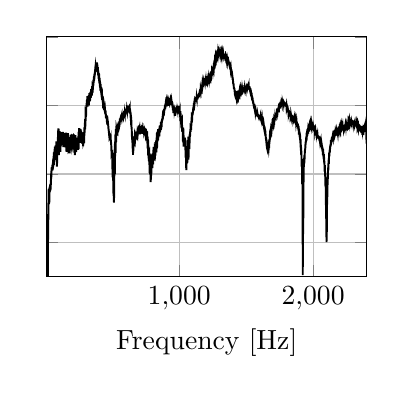
\begin{tikzpicture}

\begin{axis}[%
width=1.6in,
height=1.2in,
at={(1.011in,0.642in)},
scale only axis,
xmin=10,
xmax=2400,
xmajorgrids,
ymin=-10,
ymax=60,
ymajorgrids,
yticklabels={\empty},
xlabel={Frequency [Hz]},
axis background/.style={fill=white}
]
\addplot [color=black,solid,line width=0.7pt,forget plot]
  table[row sep=crcr]{%
0	-18.8429344080816\\
0.666675926054529	-8.84494158407596\\
1.33335185210906	3.907068627252\\
2.00002777816359	11.6090595203946\\
2.66670370421811	2.13189097085738\\
3.33337963027264	10.4221720810634\\
4.00005555632717	3.49623628005094\\
4.6667314823817	5.33794216753561\\
5.33340740843623	7.24371975140864\\
6.00008333449076	6.40813006650262\\
6.66675926054529	5.65727573948068\\
7.33343518659981	2.85209684966416\\
8.00011111265434	1.45597762238363\\
8.66678703870887	-9.30118597335561\\
9.3334629647634	-3.97830399112725\\
10.0001388908179	-4.39639751698075\\
10.6668148168725	-4.09476255222274\\
11.333490742927	-14.8486543441919\\
12.0001666689815	-11.6761628078023\\
12.666842595036	-5.71951456887732\\
13.3335185210906	-0.658420234721852\\
14.0001944471451	-5.76645170609809\\
14.6668703731996	-3.65258277735959\\
15.3335462992542	-4.80051772034599\\
16.0002222253087	-3.9589829756335\\
16.6668981513632	-20.9821735072017\\
17.3335740774177	-8.90943754478558\\
18.0002500034723	-22.9670962602259\\
18.6669259295268	0.439974337385339\\
19.3336018555813	3.36997461133588\\
20.0002777816359	1.04104453101985\\
20.6669537076904	0.863041146466912\\
21.3336296337449	8.11226737595175\\
22.0003055597994	8.69458374825248\\
22.666981485854	6.72216095608912\\
23.3336574119085	11.4966415509267\\
24.000333337963	12.0264437564795\\
24.6670092640176	12.9692772216477\\
25.3336851900721	15.7078009240285\\
26.0003611161266	14.8207480932128\\
26.6670370421811	11.2470230664094\\
27.3337129682357	14.5029848273978\\
28.0003888942902	13.5690115177866\\
28.6670648203447	12.2798363951851\\
29.3337407463993	11.4616589190787\\
30.0004166724538	13.1499212625234\\
30.6670925985083	13.4875058560669\\
31.3337685245628	15.2978526968376\\
32.0004444506174	15.5621493224007\\
32.6671203766719	16.2842990739873\\
33.3337963027264	15.1741624084043\\
34.000472228781	16.0895933390171\\
34.6671481548355	15.6673380756853\\
35.33382408089	16.1304317226485\\
36.0005000069445	16.761130518081\\
36.6671759329991	16.8184509784241\\
37.3338518590536	15.7969409081034\\
38.0005277851081	15.4422519620107\\
38.6672037111627	15.5177757759677\\
39.3338796372172	15.6345764632732\\
40.0005555632717	16.3174565670248\\
40.6672314893262	16.8687955325128\\
41.3339074153808	17.7398636961192\\
42.0005833414353	18.2065222233462\\
42.6672592674898	18.5657562262092\\
43.3339351935444	19.2654737628626\\
44.0006111195989	20.2240708600433\\
44.6672870456534	20.6001262315014\\
45.3339629717079	20.7748242110636\\
46.0006388977625	20.6961455530348\\
46.667314823817	21.3493091443735\\
47.3339907498715	21.8340524996347\\
48.0006666759261	21.1713499578826\\
48.6673426019806	21.2879508274349\\
49.3340185280351	21.9934788319142\\
50.0006944540896	21.6388241752122\\
50.6673703801442	21.7590037621221\\
51.3340463061987	21.7878592973506\\
52.0007222322532	22.5824280527068\\
52.6673981583078	21.8596435487221\\
53.3340740843623	21.930094419723\\
54.0007500104168	22.7838734872752\\
54.6674259364713	22.3215225349722\\
55.3341018625259	21.0466040466579\\
56.0007777885804	22.7916133837292\\
56.6674537146349	23.2920003416595\\
57.3341296406895	21.6089882081615\\
58.000805566744	23.4456625752669\\
58.6674814927985	24.2174303152387\\
59.334157418853	22.391248568469\\
60.0008333449076	23.4997857140652\\
60.6675092709621	24.5522637245623\\
61.3341851970166	23.435181625822\\
62.0008611230712	24.5264706063074\\
62.6675370491257	25.2487236715802\\
63.3342129751802	22.6557126006321\\
64.0008889012347	24.9901577884083\\
64.6675648272893	24.9308904611566\\
65.3342407533438	23.9209329661773\\
66.0009166793983	25.4277707584918\\
66.6675926054529	23.5396402218595\\
67.3342685315074	26.5052404642393\\
68.0009444575619	26.3426481148257\\
68.6676203836164	24.6523143504887\\
69.334296309671	27.2704921658808\\
70.0009722357255	26.2048817902905\\
70.66764816178	25.905775149931\\
71.3343240878346	27.9910892618055\\
72.0010000138891	25.2234585000175\\
72.6676759399436	26.7921845094508\\
73.3343518659981	26.4398689123446\\
74.0010277920527	26.3279181780533\\
74.6677037181072	25.8035527349148\\
75.3343796441617	26.3077932422199\\
76.0010555702163	28.3499962027918\\
76.6677314962708	24.0908834316081\\
77.3344074223253	26.6767051553818\\
78.0010833483798	26.844616346315\\
78.6677592744344	24.8857755465892\\
79.3344352004889	28.301823103824\\
80.0011111265434	26.5110143441242\\
80.667787052598	28.2041224261363\\
81.3344629786525	26.5995460211323\\
82.001138904707	29.5187538636103\\
82.6678148307615	26.9314567836421\\
83.3344907568161	27.6265720806925\\
84.0011666828706	26.1292906297972\\
84.6678426089251	25.0327434760952\\
85.3345185349797	24.6827489655959\\
86.0011944610342	23.3139688896081\\
86.6678703870887	22.1332313051663\\
87.3345463131432	23.1162982893003\\
88.0012222391978	23.4002134929317\\
88.6678981652523	23.4532846684725\\
89.3345740913068	25.9888852654454\\
90.0012500173614	26.5741976160941\\
90.6679259434159	28.0950044993131\\
91.3346018694704	28.6182451718589\\
92.0012777955249	28.4991967128809\\
92.6679537215795	28.7100083512812\\
93.334629647634	29.1073506303662\\
94.0013055736885	30.5229182652189\\
94.667981499743	29.5897259289939\\
95.3346574257976	32.6337625101919\\
96.0013333518521	30.223870339701\\
96.6680092779066	33.3319641205937\\
97.3346852039612	31.1741934949014\\
98.0013611300157	32.8345065450061\\
98.6680370560702	30.7544887354485\\
99.3347129821248	33.1470599650073\\
100.001388908179	30.6648997780048\\
100.668064834234	31.2666897167305\\
101.334740760288	31.762367336355\\
102.001416686343	25.5169830487579\\
102.668092612397	30.9456373033972\\
103.334768538452	28.3516799315347\\
104.001444464506	29.2695619962253\\
104.668120390561	30.7954410443378\\
105.334796316616	29.540993221005\\
106.00147224267	32.4853108728462\\
106.668148168725	29.1157177645989\\
107.334824094779	31.6648870076429\\
108.001500020834	30.7370236713305\\
108.668175946888	26.8964945498603\\
109.334851872943	30.7427613522993\\
110.001527798997	29.8511611623321\\
110.668203725052	30.6293380037576\\
111.334879651106	32.3944186029859\\
112.001555577161	26.477498202149\\
112.668231503215	30.2215392970929\\
113.33490742927	31.0776151428171\\
114.001583355324	29.1242916476267\\
114.668259281379	30.2554040165924\\
115.334935207433	30.6361335183687\\
116.001611133488	29.4042278048957\\
116.668287059542	30.8370888049795\\
117.334962985597	28.5973395751472\\
118.001638911652	29.0441847243163\\
118.668314837706	32.2006957797248\\
119.334990763761	30.8654149816971\\
120.001666689815	28.5780729712691\\
120.66834261587	30.2824613792598\\
121.335018541924	29.2020408875155\\
122.001694467979	29.2989980266485\\
122.668370394033	31.8324194202226\\
123.335046320088	31.8330843207774\\
124.001722246142	28.4516828783974\\
124.668398172197	29.3496098065097\\
125.335074098251	29.3740315859524\\
126.001750024306	28.8558207101026\\
126.66842595036	29.2010095758027\\
127.335101876415	31.4898295893667\\
128.001777802469	30.1561894238805\\
128.668453728524	29.8757564402124\\
129.335129654579	29.8940526627486\\
130.001805580633	30.7550647112376\\
130.668481506688	29.1646586689869\\
131.335157432742	30.7233830298356\\
132.001833358797	32.2651260015196\\
132.668509284851	31.1867003082063\\
133.335185210906	30.8522424212389\\
134.00186113696	29.7531994921268\\
134.668537063015	30.2766826214082\\
135.335212989069	27.8405196206313\\
136.001888915124	28.3038234928908\\
136.668564841178	28.8071953820231\\
137.335240767233	30.1633381500177\\
138.001916693287	29.7336231443437\\
138.668592619342	28.4648337197757\\
139.335268545396	30.9994116724969\\
140.001944471451	30.8175186811381\\
140.668620397506	31.1883449352268\\
141.33529632356	30.551224565316\\
142.001972249615	30.0736075884572\\
142.668648175669	32.0025396287026\\
143.335324101724	31.4669226006489\\
144.002000027778	31.1242075776884\\
144.668675953833	30.4706136920832\\
145.335351879887	29.3477320422998\\
146.002027805942	30.6604724805977\\
146.668703731996	29.9004592441771\\
147.335379658051	29.9702987325465\\
148.002055584105	29.5427559246445\\
148.66873151016	27.7801661820394\\
149.335407436214	30.1013920456695\\
150.002083362269	30.0868384403121\\
150.668759288323	29.7000569317369\\
151.335435214378	30.6244304700907\\
152.002111140433	29.2954554032296\\
152.668787066487	29.8789654537269\\
153.335462992542	31.3450146995981\\
154.002138918596	31.1686264434189\\
154.668814844651	32.0866336496943\\
155.335490770705	31.5607205839312\\
156.00216669676	29.6430209709442\\
156.668842622814	29.6094726242602\\
157.335518548869	27.3999611500299\\
158.002194474923	26.4442378423186\\
158.668870400978	27.8511156110568\\
159.335546327032	29.2815677572793\\
160.002222253087	29.6751803558815\\
160.668898179141	30.2290951313179\\
161.335574105196	29.4879276363474\\
162.00225003125	29.2234213673632\\
162.668925957305	31.0702984091097\\
163.335601883359	30.3082691151706\\
164.002277809414	27.8488608561871\\
164.668953735469	27.7939559145618\\
165.335629661523	28.0402354291323\\
166.002305587578	28.7358562305965\\
166.668981513632	30.2760106930511\\
167.335657439687	30.4796580377786\\
168.002333365741	29.969007984935\\
168.669009291796	30.6915786783727\\
169.33568521785	31.9003079305752\\
170.002361143905	29.9187243489736\\
170.669037069959	27.1184978734245\\
171.335712996014	28.0657872623955\\
172.002388922068	30.3757530252628\\
172.669064848123	30.3846823475822\\
173.335740774177	28.8781335962552\\
174.002416700232	27.0528307348787\\
174.669092626286	27.1109757296032\\
175.335768552341	28.424593027749\\
176.002444478396	29.5013720512392\\
176.66912040445	28.7877988811798\\
177.335796330505	27.6267174446438\\
178.002472256559	27.8030023812184\\
178.669148182614	27.5449665666331\\
179.335824108668	28.3320600529416\\
180.002500034723	29.6150061244262\\
180.669175960777	28.3609796864836\\
181.335851886832	26.0491518566697\\
182.002527812886	28.6819384734156\\
182.669203738941	29.9269253009046\\
183.335879664995	27.8589283955534\\
184.00255559105	27.4928233835593\\
184.669231517104	28.3627456233489\\
185.335907443159	29.4496917241811\\
186.002583369213	29.621736995699\\
186.669259295268	28.9896528656059\\
187.335935221323	29.4434601223753\\
188.002611147377	30.5978724270419\\
188.669287073432	30.8201137929861\\
189.335962999486	30.2497400812278\\
190.002638925541	31.5144531552819\\
190.669314851595	30.7805524733679\\
191.33599077765	30.8261868646997\\
192.002666703704	30.2965194299121\\
192.669342629759	29.8820272632289\\
193.336018555813	30.5137734818141\\
194.002694481868	27.9303245539409\\
194.669370407922	28.6469168177455\\
195.336046333977	28.5775972885376\\
196.002722260031	26.9070095559278\\
196.669398186086	30.1549907177668\\
197.33607411214	30.5749663138528\\
198.002750038195	31.5701362071571\\
198.66942596425	31.1994634075993\\
199.336101890304	30.7887442606635\\
200.002777816359	29.7913361762141\\
200.669453742413	28.7009352873217\\
201.336129668468	27.9263417906062\\
202.002805594522	28.0518266155109\\
202.669481520577	29.8138972930161\\
203.336157446631	31.4052012405897\\
204.002833372686	30.7499422819632\\
204.66950929874	31.0576776742222\\
205.336185224795	28.8747484680911\\
206.002861150849	28.4510658729898\\
206.669537076904	28.6701465761488\\
207.336213002958	29.9234138288411\\
208.002888929013	31.068705492996\\
208.669564855067	31.3160107788661\\
209.336240781122	29.9260448395067\\
210.002916707176	28.2847576451667\\
210.669592633231	28.4555630023148\\
211.336268559286	29.9616367068819\\
212.00294448534	31.604732782047\\
212.669620411395	30.309873981334\\
213.336296337449	29.0490698615691\\
214.002972263504	27.1346988740986\\
214.669648189558	29.8724125230583\\
215.336324115613	31.1319596291382\\
216.003000041667	31.097532489887\\
216.669675967722	28.88355025228\\
217.336351893776	26.2802868718139\\
218.003027819831	30.7460804433424\\
218.669703745885	30.5297883846931\\
219.33637967194	30.703021381922\\
220.003055597994	25.5011032848599\\
220.669731524049	28.3622612536161\\
221.336407450103	31.2152183813689\\
222.003083376158	30.2149146349985\\
222.669759302213	29.0065848916047\\
223.336435228267	27.8393030173705\\
224.003111154322	30.4660556234047\\
224.669787080376	31.3640875669112\\
225.336463006431	28.086815987324\\
226.003138932485	28.4492554572761\\
226.66981485854	30.2435413446823\\
227.336490784594	30.6161950258825\\
228.003166710649	27.6817188251053\\
228.669842636703	28.2525682239071\\
229.336518562758	30.5985076764449\\
230.003194488812	29.2399178776893\\
230.669870414867	26.3597529929076\\
231.336546340921	29.5793305668266\\
232.003222266976	30.2842371002653\\
232.66989819303	26.9897344210903\\
233.336574119085	28.1471828087953\\
234.00325004514	30.2597836796619\\
234.669925971194	28.181354602313\\
235.336601897249	27.9158160088277\\
236.003277823303	29.3553966477695\\
236.669953749358	28.8685077867501\\
237.336629675412	28.6358902009342\\
238.003305601467	29.151177107998\\
238.669981527521	28.0488286606784\\
239.336657453576	29.1039586247358\\
240.00333337963	28.6223454804378\\
240.670009305685	29.4880518505217\\
241.336685231739	28.52707939815\\
242.003361157794	28.266306894527\\
242.670037083848	29.436363929933\\
243.336713009903	28.6530632424862\\
244.003388935957	29.8919419601563\\
244.670064862012	30.4175366003482\\
245.336740788066	27.0809219789051\\
246.003416714121	31.0350501144498\\
246.670092640176	29.3930070790121\\
247.33676856623	29.7592730334251\\
248.003444492285	31.8036699649806\\
248.670120418339	27.3348265521758\\
249.336796344394	32.3609840981748\\
250.003472270448	29.8946620810523\\
250.670148196503	31.7929701689509\\
251.336824122557	32.1944638056823\\
252.003500048612	30.5283804538495\\
252.670175974666	33.3676224228154\\
253.336851900721	30.868642361524\\
254.003527826775	33.2126043890438\\
254.67020375283	32.4464397607355\\
255.336879678884	31.2334965910674\\
256.003555604939	32.6014253361732\\
256.670231530993	29.5145179652617\\
257.336907457048	32.4118293604858\\
258.003583383103	29.4987787554529\\
258.670259309157	31.5379713210154\\
259.336935235212	31.3027120739075\\
260.003611161266	31.378932888115\\
260.670287087321	32.4151973738197\\
261.336963013375	31.8755393375291\\
262.00363893943	33.134151100273\\
262.670314865484	30.8641050254429\\
263.336990791539	33.037989574727\\
264.003666717593	29.6215417128918\\
264.670342643648	32.1325647434013\\
265.337018569702	29.1180786711431\\
266.003694495757	31.1113502145215\\
266.670370421811	29.1869629277356\\
267.337046347866	32.6480906459668\\
268.00372227392	29.7430446290171\\
268.670398199975	32.1714647726623\\
269.33707412603	30.2460992923021\\
270.003750052084	31.1191643498608\\
270.670425978139	29.0254539856645\\
271.337101904193	30.9571980127332\\
272.003777830248	29.1460616835447\\
272.670453756302	30.8531247529323\\
273.337129682357	30.4410999473694\\
274.003805608411	31.7147130309257\\
274.670481534466	29.6856161609942\\
275.33715746052	29.3884440733776\\
276.003833386575	29.2915592971311\\
276.670509312629	28.8378453701689\\
277.337185238684	29.7883852465385\\
278.003861164738	29.900866430606\\
278.670537090793	30.7629918973219\\
279.337213016847	28.9183732941536\\
280.003888942902	28.8944541577153\\
280.670564868956	29.5394818091163\\
281.337240795011	30.0237685722209\\
282.003916721066	30.3354742040549\\
282.67059264712	28.1765245911029\\
283.337268573175	28.5801833864376\\
284.003944499229	29.9254358237851\\
284.670620425284	30.1935608542207\\
285.337296351338	32.2460998435289\\
286.003972277393	29.6799904117181\\
286.670648203447	29.7936347270443\\
287.337324129502	30.9613145735549\\
288.004000055556	30.4062816076104\\
288.670675981611	32.0690070600166\\
289.337351907665	31.4789899855028\\
290.00402783372	29.0154727165523\\
290.670703759774	32.1665210647843\\
291.337379685829	33.5716259016251\\
292.004055611883	32.5259354082854\\
292.670731537938	32.4592822956855\\
293.337407463993	32.3246098366\\
294.004083390047	32.6222840265406\\
294.670759316102	34.0180280319283\\
295.337435242156	34.960472734722\\
296.004111168211	33.9566974685778\\
296.670787094265	33.0270086972922\\
297.33746302032	35.5309499066603\\
298.004138946374	36.0951236020633\\
298.670814872429	33.9134408983699\\
299.337490798483	34.4144495254164\\
300.004166724538	37.19611592523\\
300.670842650592	37.0698020100338\\
301.337518576647	35.5101596729711\\
302.004194502701	36.4897803897812\\
302.670870428756	38.2196251364824\\
303.33754635481	37.876284032482\\
304.004222280865	37.0391310600794\\
304.67089820692	38.0595143807013\\
305.337574132974	39.5154740828177\\
306.004250059029	39.7857686375634\\
306.670925985083	39.4644220926583\\
307.337601911138	40.1196271150872\\
308.004277837192	40.2956400667265\\
308.670953763247	40.0239651146064\\
309.337629689301	41.1364733972345\\
310.004305615356	41.5223855306092\\
310.67098154141	40.4094774381043\\
311.337657467465	40.561826545805\\
312.004333393519	41.7688870474222\\
312.671009319574	41.000701921682\\
313.337685245628	41.1945092268295\\
314.004361171683	42.7124067887137\\
314.671037097737	42.045891399169\\
315.337713023792	39.6477014573053\\
316.004388949847	41.7678664623993\\
316.671064875901	42.0334165571405\\
317.337740801956	41.0635298146773\\
318.00441672801	42.0559408933319\\
318.671092654065	42.7334289675683\\
319.337768580119	41.8223743825168\\
320.004444506174	42.8235274363415\\
320.671120432228	42.2886564447346\\
321.337796358283	40.0238521852387\\
322.004472284337	42.2912013308153\\
322.671148210392	42.4715507400187\\
323.337824136446	41.0861441741469\\
324.004500062501	42.482821298788\\
324.671175988555	40.1693457915656\\
325.33785191461	40.6477914570679\\
326.004527840664	42.3574995011084\\
326.671203766719	42.2039390147656\\
327.337879692774	42.6109532555612\\
328.004555618828	43.2035010898828\\
328.671231544883	41.3870514298359\\
329.337907470937	43.5718799452956\\
330.004583396992	43.2472252151248\\
330.671259323046	42.6971874329996\\
331.337935249101	43.3559666463266\\
332.004611175155	41.2051221838892\\
332.67128710121	42.5396466655099\\
333.337963027264	42.1974539163008\\
334.004638953319	41.5232360012341\\
334.671314879373	42.7330863908283\\
335.337990805428	42.528964011806\\
336.004666731482	43.9755052214405\\
336.671342657537	43.2544242976938\\
337.338018583591	42.684689877653\\
338.004694509646	43.6988638315066\\
338.671370435701	42.1971980971956\\
339.338046361755	43.0599728728764\\
340.00472228781	42.2819821850606\\
340.671398213864	43.78919936633\\
341.338074139919	44.8003892158893\\
342.004750065973	43.0153636254729\\
342.671425992028	44.4368050778638\\
343.338101918082	42.7905500369862\\
344.004777844137	43.4722142860698\\
344.671453770191	42.8418537351459\\
345.338129696246	44.0218856790206\\
346.0048056223	44.3447475900996\\
346.671481548355	43.1719623025317\\
347.338157474409	44.4178252647274\\
348.004833400464	42.9259312224293\\
348.671509326518	44.6542412229939\\
349.338185252573	44.4051738230658\\
350.004861178627	45.6024548510286\\
350.671537104682	43.5885468243998\\
351.338213030737	45.3623382072631\\
352.004888956791	44.8705387522676\\
352.671564882846	45.6992397369553\\
353.3382408089	45.6338041612754\\
354.004916734955	45.15980667694\\
354.671592661009	45.0991015810892\\
355.338268587064	46.0510262804429\\
356.004944513118	46.3650896598473\\
356.671620439173	45.8602937062166\\
357.338296365227	45.5659597246794\\
358.004972291282	46.6075435228596\\
358.671648217336	47.4111388291515\\
359.338324143391	45.8341431372864\\
360.005000069445	46.7893653950727\\
360.6716759955	46.9989536044353\\
361.338351921554	47.6293056891234\\
362.005027847609	47.1418631176181\\
362.671703773664	47.3101267866553\\
363.338379699718	48.5475784282497\\
364.005055625773	47.3173256792727\\
364.671731551827	48.0987378344693\\
365.338407477882	47.6817051720608\\
366.005083403936	49.0715117164896\\
366.671759329991	47.8342367150429\\
367.338435256045	49.0863247268338\\
368.0051111821	48.4978506115855\\
368.671787108154	49.3226339826415\\
369.338463034209	48.9796700712608\\
370.005138960263	49.8254161659425\\
370.671814886318	49.189511071971\\
371.338490812372	49.5965044407079\\
372.005166738427	50.5531371856027\\
372.671842664481	49.681000981831\\
373.338518590536	51.3294551123575\\
374.005194516591	49.8332532446957\\
374.671870442645	51.7127087964686\\
375.3385463687	50.1757432218729\\
376.005222294754	51.8773136994741\\
376.671898220809	50.5345161708454\\
377.338574146863	51.4625188319924\\
378.005250072918	51.3167668359686\\
378.671925998972	50.8930998600828\\
379.338601925027	52.0192717962724\\
380.005277851081	51.335341519275\\
380.671953777136	52.0009281738771\\
381.33862970319	51.9974444408241\\
382.005305629245	51.1596900914597\\
382.671981555299	52.0174592258563\\
383.338657481354	51.1335367937671\\
384.005333407408	51.4187045386292\\
384.672009333463	52.1073301730599\\
385.338685259517	50.6912637233557\\
386.005361185572	52.5376953576097\\
386.672037111627	50.8071769648767\\
387.338713037681	50.8072062430175\\
388.005388963736	51.8385969486242\\
388.67206488979	50.0232595054154\\
389.338740815845	51.5739372575639\\
390.005416741899	50.9992924056756\\
390.672092667954	49.8907588256942\\
391.338768594008	50.8484723702121\\
392.005444520063	49.9869200278701\\
392.672120446117	49.7580591586546\\
393.338796372172	51.175080938037\\
394.005472298226	48.8340424321688\\
394.672148224281	49.4583281798769\\
395.338824150335	50.037265134718\\
396.00550007639	48.7038285685603\\
396.672176002444	49.3412688316014\\
397.338851928499	49.3564766399959\\
398.005527854554	47.8521096981271\\
398.672203780608	48.9562278036037\\
399.338879706663	49.3468276985386\\
400.005555632717	47.6528147335053\\
400.672231558772	48.0821762729584\\
401.338907484826	49.2037638006468\\
402.005583410881	47.1025791537586\\
402.672259336935	47.8268005150409\\
403.33893526299	47.9847383862076\\
404.005611189044	46.5934021673235\\
404.672287115099	46.4415436738994\\
405.338963041153	48.0040153470907\\
406.005638967208	47.0124672087565\\
406.672314893262	45.5649070131276\\
407.338990819317	46.6381079815779\\
408.005666745371	47.21451166879\\
408.672342671426	45.6339417723795\\
409.339018597481	45.2264162300014\\
410.005694523535	46.7889801147224\\
410.67237044959	45.7749254469178\\
411.339046375644	44.3693962093801\\
412.005722301699	45.3716672966012\\
412.672398227753	45.7260170408393\\
413.339074153808	44.5594652010318\\
414.005750079862	44.1997908821746\\
414.672426005917	45.156136224364\\
415.339101931971	44.9868054025995\\
416.005777858026	43.9697750735489\\
416.67245378408	43.9000355951566\\
417.339129710135	44.0646345878489\\
418.005805636189	43.7877052853524\\
418.672481562244	43.1733080079888\\
419.339157488298	43.4062581791957\\
420.005833414353	44.0337013450954\\
420.672509340407	43.4102154632678\\
421.339185266462	42.0851205116545\\
422.005861192517	42.4397960310918\\
422.672537118571	43.2454435378208\\
423.339213044626	43.3442932577799\\
424.00588897068	42.5474034119659\\
424.672564896735	41.6251706417696\\
425.339240822789	42.0940450061338\\
426.005916748844	42.7875816512836\\
426.672592674898	42.2960536036048\\
427.339268600953	41.5423330252989\\
428.005944527007	41.3771503441748\\
428.672620453062	41.7417499184261\\
429.339296379116	42.0347348995167\\
430.005972305171	41.1832627215462\\
430.672648231225	40.2582620527076\\
431.33932415728	40.3144232720003\\
432.006000083334	41.0448142490602\\
432.672676009389	41.6220176128709\\
433.339351935444	41.1045225616876\\
434.006027861498	40.0820851423136\\
434.672703787553	39.7949756084911\\
435.339379713607	40.5281824428611\\
436.006055639662	40.5810555175867\\
436.672731565716	40.3228634812306\\
437.339407491771	39.7331784878231\\
438.006083417825	38.7490340382592\\
438.67275934388	38.9154660100518\\
439.339435269934	39.378419719744\\
440.006111195989	39.9254561644455\\
440.672787122043	39.7644214821191\\
441.339463048098	39.0473046019997\\
442.006138974152	38.5213689902178\\
442.672814900207	38.3248677240061\\
443.339490826261	38.8662670421472\\
444.006166752316	39.2253102318046\\
444.672842678371	39.3424571751584\\
445.339518604425	39.0145655212094\\
446.00619453048	38.6178123074287\\
446.672870456534	37.8705888194655\\
447.339546382589	37.7106542829074\\
448.006222308643	37.4206453411843\\
448.672898234698	37.9120589478237\\
449.339574160752	38.1928504160038\\
450.006250086807	38.4630224092452\\
450.672926012861	38.1088018675204\\
451.339601938916	37.6937514407508\\
452.00627786497	36.9815184543972\\
452.672953791025	36.5336768089025\\
453.339629717079	36.4899674428975\\
454.006305643134	36.6517488406688\\
454.672981569188	36.8758104075931\\
455.339657495243	36.9231821434128\\
456.006333421298	37.1853495182967\\
456.673009347352	36.908755190899\\
457.339685273407	36.8781225100017\\
458.006361199461	36.4087234875141\\
458.673037125516	36.0980345654716\\
459.33971305157	35.6144481882991\\
460.006388977625	35.2941044362929\\
460.673064903679	35.1363875839739\\
461.339740829734	34.961944077296\\
462.006416755788	34.9933038159141\\
462.673092681843	34.9729798038799\\
463.339768607897	35.3539187951738\\
464.006444533952	35.2514323939225\\
464.673120460006	35.4598809466291\\
465.339796386061	35.5552521847408\\
466.006472312115	35.3249862795567\\
466.67314823817	35.3013464811467\\
467.339824164225	34.974954881513\\
468.006500090279	34.7492319820285\\
468.673176016334	34.5784588194354\\
469.339851942388	34.246712977487\\
470.006527868443	33.9784771100941\\
470.673203794497	33.7186629259853\\
471.339879720552	33.2857638336816\\
472.006555646606	33.1194378159598\\
472.673231572661	32.8895496458257\\
473.339907498715	32.6708416374446\\
474.00658342477	32.5534186363848\\
474.673259350824	32.2957546468315\\
475.339935276879	32.0017486544819\\
476.006611202933	31.8843543053765\\
476.673287128988	31.4788987683949\\
477.339963055042	31.4888772976838\\
478.006638981097	31.6879731372179\\
478.673314907152	30.8962478664373\\
479.339990833206	30.9722896412259\\
480.006666759261	31.0245499046301\\
480.673342685315	30.7834751010897\\
481.34001861137	30.6200687938059\\
482.006694537424	30.5980840294981\\
482.673370463479	30.0653295144498\\
483.340046389533	30.9135540379168\\
484.006722315588	30.3654192421742\\
484.673398241642	29.8425326850856\\
485.340074167697	30.6514183879776\\
486.006750093751	30.0284663202936\\
486.673426019806	30.3717747752991\\
487.34010194586	30.0827834015526\\
488.006777871915	29.889844302519\\
488.673453797969	30.0506753363562\\
489.340129724024	29.480430839226\\
490.006805650078	29.941796390442\\
490.673481576133	29.2483399078049\\
491.340157502188	28.5014402144146\\
492.006833428242	28.8187075553365\\
492.673509354297	26.9976438057228\\
493.340185280351	28.2173228244244\\
494.006861206406	26.4986988078874\\
494.67353713246	26.6112071891905\\
495.340213058515	26.3763985643643\\
496.006888984569	25.9748820059484\\
496.673564910624	25.1988510126762\\
497.340240836678	26.5610894037211\\
498.006916762733	25.6357100173118\\
498.673592688787	26.2926770652346\\
499.340268614842	26.3265184243126\\
500.006944540896	24.4264834739024\\
500.673620466951	26.1357856314872\\
501.340296393005	21.4637414712454\\
502.00697231906	24.0538599613789\\
502.673648245115	18.9965641318293\\
503.340324171169	23.4400062403474\\
504.007000097224	19.2582831739636\\
504.673676023278	23.2608430401331\\
505.340351949333	21.4412835643564\\
506.007027875387	18.9184418792552\\
506.673703801442	21.550323355725\\
507.340379727496	14.3877542708197\\
508.007055653551	19.4756082102673\\
508.673731579605	15.5597365275519\\
509.34040750566	18.7751236928634\\
510.007083431714	13.6336937931002\\
510.673759357769	21.4905362187199\\
511.340435283823	11.8165510580541\\
512.007111209878	24.0036350656541\\
512.673787135932	11.6817646370705\\
513.340463061987	21.3307445319319\\
514.007138988041	13.0639442693756\\
514.673814914096	21.0761223907598\\
515.340490840151	19.3724131408841\\
516.007166766205	23.9765507527709\\
516.67384269226	26.2259570309124\\
517.340518618314	21.7861940449567\\
518.007194544369	25.6229360136534\\
518.673870470423	25.7508762756939\\
519.340546396478	19.996435224463\\
520.007222322532	28.7159694711825\\
520.673898248587	29.4518059124699\\
521.340574174641	25.1224599814455\\
522.007250100696	29.5633209103387\\
522.67392602675	27.1925556145375\\
523.340601952805	30.7380204831855\\
524.007277878859	31.7336243993215\\
524.673953804914	26.1431769887471\\
525.340629730968	30.2855113327411\\
526.007305657023	32.504719359115\\
526.673981583078	29.2388543856452\\
527.340657509132	33.0882442265437\\
528.007333435187	32.721998422916\\
528.674009361241	29.3746015296348\\
529.340685287296	31.9556664924697\\
530.00736121335	33.9767474005074\\
530.674037139405	31.2231106044943\\
531.340713065459	31.2700642514311\\
532.007388991514	33.2918605065748\\
532.674064917568	33.1730496090311\\
533.340740843623	32.7125412485969\\
534.007416769677	32.9467660166733\\
534.674092695732	33.742429648859\\
535.340768621786	33.3692354320208\\
536.007444547841	33.0834085658005\\
536.674120473896	32.9868562360398\\
537.34079639995	33.5524237131814\\
538.007472326005	33.6437808387699\\
538.674148252059	32.7944225353098\\
539.340824178114	32.7083780290029\\
540.007500104168	33.5929898247006\\
540.674176030223	34.1529711180493\\
541.340851956277	32.882028039382\\
542.007527882332	32.1895302556053\\
542.674203808386	33.1926672191381\\
543.340879734441	34.5942629670676\\
544.007555660495	33.9464752503382\\
544.67423158655	32.2624889887063\\
545.340907512604	33.7263359378066\\
546.007583438659	34.7628320892086\\
546.674259364713	33.9698503970178\\
547.340935290768	33.9665182275379\\
548.007611216823	34.0823411479785\\
548.674287142877	33.3317408400059\\
549.340963068932	33.0556196150262\\
550.007638994986	34.4046432232879\\
550.674314921041	34.6570894171478\\
551.340990847095	34.1162502534894\\
552.00766677315	34.1103678732309\\
552.674342699204	34.5354485927489\\
553.341018625259	33.8611950731422\\
554.007694551313	34.1297370708812\\
554.674370477368	35.2777711244412\\
555.341046403422	35.1045369337794\\
556.007722329477	35.3022548269242\\
556.674398255531	36.170790913282\\
557.341074181586	35.3251979817401\\
558.00775010764	35.4491064357091\\
558.674426033695	36.1095743207834\\
559.341101959749	35.0788061776694\\
560.007777885804	35.4265472869434\\
560.674453811858	36.0146239975707\\
561.341129737913	35.4343096441938\\
562.007805663968	35.77553803628\\
562.674481590022	36.542214339882\\
563.341157516077	36.0317652832083\\
564.007833442131	36.6628154781468\\
564.674509368186	36.6936085254874\\
565.34118529424	36.0208750968629\\
566.007861220295	37.1137053492086\\
566.674537146349	36.7656745408641\\
567.341213072404	36.7939898921484\\
568.007888998458	37.377277810714\\
568.674564924513	36.641666519827\\
569.341240850567	36.9522139173856\\
570.007916776622	37.0628754498012\\
570.674592702676	36.4135024295506\\
571.341268628731	37.2774833075617\\
572.007944554785	36.6695497012667\\
572.67462048084	36.8980384537642\\
573.341296406895	37.3388883560895\\
574.007972332949	36.6073415626129\\
574.674648259004	37.4541423127372\\
575.341324185058	36.8739965082768\\
576.008000111113	37.0182950642317\\
576.674676037167	37.3203960678024\\
577.341351963222	36.5899787594273\\
578.008027889276	37.3610914925705\\
578.674703815331	36.7134551343309\\
579.341379741385	37.499890689111\\
580.00805566744	37.1365107654789\\
580.674731593494	37.0174038586226\\
581.341407519549	37.5533652340793\\
582.008083445603	36.7840255670139\\
582.674759371658	37.8032991329715\\
583.341435297712	36.9456988464037\\
584.008111223767	37.5540669430412\\
584.674787149822	37.3003949268057\\
585.341463075876	37.3099104896853\\
586.008139001931	37.4893993723853\\
586.674814927985	37.4207435195018\\
587.34149085404	37.9154633960864\\
588.008166780094	37.1010962889826\\
588.674842706149	37.8755263399902\\
589.341518632203	37.1004155790719\\
590.008194558258	37.8379074486706\\
590.674870484312	37.3045939742317\\
591.341546410367	37.9707837359434\\
592.008222336421	37.2717733038612\\
592.674898262476	38.010610510688\\
593.34157418853	37.4398797928589\\
594.008250114585	37.8586164088877\\
594.674926040639	37.6860615279336\\
595.341601966694	38.1189987295134\\
596.008277892749	37.5515893429949\\
596.674953818803	38.1070130161145\\
597.341629744858	37.7681900657086\\
598.008305670912	38.3202887108478\\
598.674981596967	37.9849039929729\\
599.341657523021	37.914546672696\\
600.008333449076	38.1310320125686\\
600.67500937513	38.5571505485666\\
601.341685301185	37.598342169115\\
602.008361227239	38.6773924003577\\
602.675037153294	38.004590482945\\
603.341713079348	38.904560243106\\
604.008389005403	37.991013220186\\
604.675064931457	38.8169017139068\\
605.341740857512	38.4291530727042\\
606.008416783566	38.8238654673094\\
606.675092709621	38.550711722368\\
607.341768635676	38.8335241726424\\
608.00844456173	38.8169889511116\\
608.675120487785	38.7860358418935\\
609.341796413839	39.0815059114297\\
610.008472339894	38.9345285396075\\
610.675148265948	38.9415216970259\\
611.341824192003	38.7799610866837\\
612.008500118057	39.3956065128983\\
612.675176044112	38.6065937982696\\
613.341851970166	39.5401583731317\\
614.008527896221	38.9183785117537\\
614.675203822275	38.866230799026\\
615.34187974833	39.5752387229249\\
616.008555674384	38.3728869590924\\
616.675231600439	39.9465897543381\\
617.341907526493	38.6032647673825\\
618.008583452548	39.5743889968956\\
618.675259378603	39.2062047744186\\
619.341935304657	38.8116478991804\\
620.008611230711	39.570909686746\\
620.675287156766	38.6120274509041\\
621.341963082821	39.5611073572074\\
622.008639008875	38.8444595405949\\
622.67531493493	39.2142139511604\\
623.341990860984	39.2825774239556\\
624.008666787039	39.0029726170196\\
624.675342713093	38.9970123928559\\
625.342018639148	39.4185763135859\\
626.008694565202	38.4688774297461\\
626.675370491257	39.3234274449711\\
627.342046417311	38.5531055435941\\
628.008722343366	38.8046205974729\\
628.67539826942	39.0092196961621\\
629.342074195475	38.3970885340226\\
630.008750121529	38.6906440857873\\
630.675426047584	38.8274149404208\\
631.342101973638	37.666931217261\\
632.008777899693	39.1429187609113\\
632.675453825748	37.9837530583695\\
633.342129751802	37.9843792234104\\
634.008805677857	38.771544177564\\
634.675481603911	37.4617312828796\\
635.342157529966	37.8577470034772\\
636.00883345602	38.2121582499989\\
636.675509382075	37.4412900188713\\
637.342185308129	36.4705741213086\\
638.008861234184	37.6783218345115\\
638.675537160238	35.8664617348301\\
639.342213086293	35.5116784362106\\
640.008889012347	36.7427206370712\\
640.675564938402	34.8953841808732\\
641.342240864456	34.3794310691927\\
642.008916790511	35.721893921253\\
642.675592716565	34.2926637588607\\
643.34226864262	33.840846875875\\
644.008944568675	33.0744588062082\\
644.675620494729	33.6749433217837\\
645.342296420784	33.1988634444004\\
646.008972346838	30.8814946268436\\
646.675648272893	31.4135295964048\\
647.342324198947	32.417676067011\\
648.009000125002	30.385982702976\\
648.675676051056	30.0665150890799\\
649.342351977111	31.1704891497593\\
650.009027903165	30.7000599752403\\
650.67570382922	29.3387131037375\\
651.342379755274	28.324459486754\\
652.009055681329	27.4979811915939\\
652.675731607383	30.1481935820891\\
653.342407533438	30.8470080440179\\
654.009083459492	28.5759270781698\\
654.675759385547	25.6257231493269\\
655.342435311602	28.5341260831335\\
656.009111237656	30.2661909251636\\
656.675787163711	29.7565464945682\\
657.342463089765	28.742621968856\\
658.00913901582	28.8035897196987\\
658.675814941874	29.0355534837727\\
659.342490867929	28.870861980404\\
660.009166793983	29.4080395962155\\
660.675842720038	30.4463655774758\\
661.342518646092	30.9694186638159\\
662.009194572147	29.1742426659306\\
662.675870498201	28.1059761262438\\
663.342546424256	29.543076346049\\
664.00922235031	29.9735901491995\\
664.675898276365	30.4744412963053\\
665.342574202419	30.531838626846\\
666.009250128474	29.9855237938402\\
666.675926054529	29.470144415199\\
667.342601980583	29.8558574043006\\
668.009277906638	29.6563328060187\\
668.675953832692	29.5620139820404\\
669.342629758747	30.2986975727838\\
670.009305684801	31.1274185246032\\
670.675981610856	31.9711097095484\\
671.34265753691	31.9041916028891\\
672.009333462965	31.837019627602\\
672.676009389019	31.8326781757805\\
673.342685315074	31.6521668196417\\
674.009361241128	31.6831217535496\\
674.676037167183	31.089655550795\\
675.342713093237	30.7256228033234\\
676.009389019292	30.5970906029459\\
676.676064945346	30.5734570704227\\
677.342740871401	30.9780398557597\\
678.009416797456	31.6570847582376\\
678.67609272351	31.3350690080168\\
679.342768649565	31.0906722148842\\
680.009444575619	30.1852469729081\\
680.676120501674	30.4771209022651\\
681.342796427728	30.5259388587446\\
682.009472353783	31.5348665198834\\
682.676148279837	31.5722073865918\\
683.342824205892	31.6956368140475\\
684.009500131946	31.0538085376959\\
684.676176058001	30.9316181408239\\
685.342851984055	31.043010804693\\
686.00952791011	31.3722021865709\\
686.676203836164	31.6962123216079\\
687.342879762219	32.0046544627666\\
688.009555688273	31.8554507013098\\
688.676231614328	31.4758374285094\\
689.342907540382	31.3564440446898\\
690.009583466437	31.6312870676452\\
690.676259392492	31.8751792853951\\
691.342935318546	32.50489055484\\
692.009611244601	32.7241203546257\\
692.676287170655	33.3088084306096\\
693.34296309671	33.0777980634691\\
694.009639022764	33.4919753859938\\
694.676314948819	32.621667909648\\
695.342990874873	32.6812393279935\\
696.009666800928	32.4086505240744\\
696.676342726982	32.1175276036068\\
697.343018653037	32.102533532745\\
698.009694579091	31.7527303092798\\
698.676370505146	32.6328829746678\\
699.3430464312	33.4761749929837\\
700.009722357255	33.4407436932402\\
700.676398283309	33.0746074211852\\
701.343074209364	32.7417405164545\\
702.009750135419	32.4558078820108\\
702.676426061473	33.058378797223\\
703.343101987528	33.5040299846632\\
704.009777913582	33.6154178408765\\
704.676453839637	33.3570716247984\\
705.343129765691	32.7526100584496\\
706.009805691746	32.2047850048591\\
706.6764816178	31.5522398340791\\
707.343157543855	32.3308384549367\\
708.009833469909	33.8708782209868\\
708.676509395964	33.5677392776652\\
709.343185322018	31.7883054949117\\
710.009861248073	32.0813660066931\\
710.676537174127	32.9269436197855\\
711.343213100182	33.4009976353901\\
712.009889026236	33.4380600489671\\
712.676564952291	32.9960415127969\\
713.343240878346	32.5181045348182\\
714.0099168044	32.8436922036318\\
714.676592730455	33.9352291021335\\
715.343268656509	33.6268510792837\\
716.009944582564	32.3710560019102\\
716.676620508618	33.2424495347342\\
717.343296434673	33.9280189954054\\
718.009972360727	32.8102348282939\\
718.676648286782	33.0133186851399\\
719.343324212836	33.1816665802285\\
720.010000138891	33.2640693368149\\
720.676676064945	33.3565430182534\\
721.343351991	32.4759345896375\\
722.010027917054	32.9840908459292\\
722.676703843109	33.0435826944375\\
723.343379769163	32.4442801510751\\
724.010055695218	33.0162173751069\\
724.676731621273	33.2117053584189\\
725.343407547327	31.7505541729931\\
726.010083473382	32.864984551237\\
726.676759399436	32.6461942005901\\
727.343435325491	32.6520598369977\\
728.010111251545	32.9039837969254\\
728.6767871776	32.5690663526879\\
729.343463103654	32.8493065548139\\
730.010139029709	32.7467890604993\\
730.676814955763	33.8152661034755\\
731.343490881818	32.6774804787076\\
732.010166807872	33.728937344907\\
732.676842733927	33.0301357066835\\
733.343518659981	33.0177210548859\\
734.010194586036	33.6422664585522\\
734.67687051209	32.262039893447\\
735.343546438145	33.5208595043034\\
736.0102223642	32.1385186658715\\
736.676898290254	32.6909211040876\\
737.343574216309	32.2595050175939\\
738.010250142363	32.3674431857286\\
738.676926068418	32.1617028438581\\
739.343601994472	32.7582737974208\\
740.010277920527	32.6450714242728\\
740.676953846581	33.2005804820337\\
741.343629772636	32.8391996349351\\
742.01030569869	33.3512403816982\\
742.676981624745	32.3525425179619\\
743.343657550799	33.0680815833328\\
744.010333476854	31.8289392342713\\
744.677009402908	32.4817433306025\\
745.343685328963	31.616981653044\\
746.010361255017	32.719163468611\\
746.677037181072	32.6521598086975\\
747.343713107127	33.0736444945334\\
748.010389033181	33.0567367485438\\
748.677064959236	31.7751509357205\\
749.34374088529	31.4562499505917\\
750.010416811345	31.5766491897296\\
750.677092737399	31.4157169438264\\
751.343768663454	33.1459364503783\\
752.010444589508	32.0630979886163\\
752.677120515563	32.7658161793481\\
753.343796441617	31.1943047498544\\
754.010472367672	30.8645562270613\\
754.677148293726	30.4385505739122\\
755.343824219781	31.1708547101916\\
756.010500145835	32.4804191341197\\
756.67717607189	31.6366578982124\\
757.343851997944	30.8188863306388\\
758.010527923999	29.7531744223906\\
758.677203850054	30.3776438791905\\
759.343879776108	30.1885708119505\\
760.010555702162	32.4044446969764\\
760.677231628217	30.912428272266\\
761.343907554272	29.1645257436519\\
762.010583480326	29.4507515660441\\
762.677259406381	28.925210698863\\
763.343935332435	30.9009981524993\\
764.01061125849	30.5573164207988\\
764.677287184544	27.5497755549969\\
765.343963110599	27.5121331921373\\
766.010639036653	29.0221973100451\\
766.677314962708	30.1098661085206\\
767.343990888762	29.5445450712363\\
768.010666814817	26.5208288071313\\
768.677342740871	26.5679557499855\\
769.344018666926	28.2723250947245\\
770.01069459298	27.853988155448\\
770.677370519035	26.936092745308\\
771.344046445089	24.6019674924039\\
772.010722371144	26.0896895407029\\
772.677398297199	27.3441216918982\\
773.344074223253	27.316789992093\\
774.010750149308	23.6999502458393\\
774.677426075362	24.3186491032622\\
775.344102001417	25.9712503430776\\
776.010777927471	26.0621579686114\\
776.677453853526	22.6901824655626\\
777.34412977958	23.0513793664827\\
778.010805705635	25.504965019042\\
778.677481631689	24.6591366877946\\
779.344157557744	20.3053795711025\\
780.010833483798	23.635408425983\\
780.677509409853	23.7438739688341\\
781.344185335907	20.286844328971\\
782.010861261962	20.0719309804245\\
782.677537188016	24.7783429900858\\
783.344213114071	23.7157690580218\\
784.010889040126	19.7380472960066\\
784.67756496618	21.6137316874309\\
785.344240892235	21.9523084882754\\
786.010916818289	19.0332911956768\\
786.677592744344	17.6382307827148\\
787.344268670398	22.5966738187169\\
788.010944596453	20.0724416308765\\
788.677620522507	18.3572016136354\\
789.344296448562	21.984786490793\\
790.010972374616	21.7671703156862\\
790.677648300671	19.4676680630923\\
791.344324226725	20.2625761515732\\
792.01100015278	23.7420118806457\\
792.677676078834	21.8511110267711\\
793.344352004889	23.2600987708604\\
794.011027930943	25.7055824091764\\
794.677703856998	24.2083352153316\\
795.344379783053	24.0059782659986\\
796.011055709107	24.7980703762758\\
796.677731635162	22.57593177494\\
797.344407561216	22.2973110764608\\
798.011083487271	23.487981194597\\
798.677759413325	21.7627800110425\\
799.34443533938	21.9083868868356\\
800.011111265434	24.8813190539357\\
800.677787191489	24.217588542444\\
801.344463117543	24.7381669066891\\
802.011139043598	25.9843981420826\\
802.677814969652	24.473946415243\\
803.344490895707	25.075129574763\\
804.011166821761	25.5099212638439\\
804.677842747816	22.8129600843171\\
805.34451867387	25.3565958172011\\
806.011194599925	24.9840227815738\\
806.67787052598	25.117431272171\\
807.344546452034	27.0260419327545\\
808.011222378089	26.3376885009711\\
808.677898304143	27.2437287285548\\
809.344574230198	27.9073201285405\\
810.011250156252	25.4740421381234\\
810.677926082307	26.4744046847144\\
811.344602008361	25.2130618712821\\
812.011277934416	25.2110259810253\\
812.67795386047	25.8148647959347\\
813.344629786525	24.8957810285622\\
814.011305712579	27.0998714187304\\
814.677981638634	27.7330357905736\\
815.344657564688	26.9267104376684\\
816.011333490743	27.2747256931624\\
816.678009416797	23.8999852383814\\
817.344685342852	26.3103105949736\\
818.011361268907	26.1850774445563\\
818.678037194961	28.1368654545079\\
819.344713121016	28.7385730512431\\
820.01138904707	25.3289125305581\\
820.678064973125	25.6745608013001\\
821.344740899179	25.4332362393635\\
822.011416825234	29.307855549655\\
822.678092751288	27.9684301890763\\
823.344768677343	27.9228889101149\\
824.011444603397	27.8044044721929\\
824.678120529452	27.3757257133775\\
825.344796455506	28.0405012019897\\
826.011472381561	28.0350043436645\\
826.678148307615	29.2861472909753\\
827.34482423367	26.9129794831154\\
828.011500159724	29.7145140084918\\
828.678176085779	29.2979812074854\\
829.344852011833	29.8333424624606\\
830.011527937888	26.2930565207778\\
830.678203863943	29.5840052373057\\
831.344879789997	30.5914977813549\\
832.011555716052	29.7507186677859\\
832.678231642106	28.097958248608\\
833.344907568161	30.4818460683172\\
834.011583494215	30.3793098234804\\
834.67825942027	30.1963221073903\\
835.344935346324	30.4015813611789\\
836.011611272379	30.2101277114485\\
836.678287198433	30.0543518095881\\
837.344963124488	30.6673524361714\\
838.011639050542	31.3245443488782\\
838.678314976597	31.1115194215433\\
839.344990902651	29.570732786544\\
840.011666828706	31.5192814144115\\
840.67834275476	31.7262711489199\\
841.345018680815	30.3864132172467\\
842.01169460687	30.5397718383058\\
842.678370532924	33.064016793348\\
843.345046458979	29.8701450175195\\
844.011722385033	32.1716462151041\\
844.678398311088	31.2764341280298\\
845.345074237142	32.0555521299864\\
846.011750163197	32.2816126672972\\
846.678426089251	31.3528358217561\\
847.345102015306	32.1882359314452\\
848.01177794136	33.1198322765016\\
848.678453867415	31.350165477216\\
849.345129793469	32.7765719894441\\
850.011805719524	32.014842367053\\
850.678481645578	32.1170489700391\\
851.345157571633	33.3481654110331\\
852.011833497687	31.0048185257132\\
852.678509423742	33.8795174295053\\
853.345185349797	32.431901718805\\
854.011861275851	32.7817498161829\\
854.678537201906	33.0143421795941\\
855.34521312796	32.1248033536506\\
856.011889054015	34.1766924282744\\
856.678564980069	32.2479476591639\\
857.345240906124	33.5672251420147\\
858.011916832178	32.4370955748892\\
858.678592758233	33.7797781767657\\
859.345268684287	33.6072071104677\\
860.011944610342	33.5979173734272\\
860.678620536396	32.7965653596897\\
861.345296462451	33.4891712143997\\
862.011972388505	33.1433288452756\\
862.67864831456	35.1262875140008\\
863.345324240614	32.9179105437464\\
864.012000166669	34.7465343168765\\
864.678676092724	33.1277351337018\\
865.345352018778	34.7468842566913\\
866.012027944833	33.8736232480748\\
866.678703870887	35.2588301996018\\
867.345379796942	33.9900651896928\\
868.012055722996	35.4869971875681\\
868.678731649051	33.7108162173899\\
869.345407575105	35.519791642324\\
870.01208350116	35.0169683996187\\
870.678759427214	35.3419486898389\\
871.345435353269	36.0666582688523\\
872.012111279323	35.6082759376239\\
872.678787205378	35.6084287712941\\
873.345463131432	35.6614115818391\\
874.012139057487	35.9057086636803\\
874.678814983541	35.6525504504876\\
875.345490909596	36.4019237796332\\
876.012166835651	36.824284702364\\
876.678842761705	35.8440795644811\\
877.34551868776	37.2470150957776\\
878.012194613814	36.9709029746597\\
878.678870539869	36.1894648952683\\
879.345546465923	37.6368067928444\\
880.012222391978	36.8611362219207\\
880.678898318032	36.8795892868377\\
881.345574244087	38.0841619180076\\
882.012250170141	37.1337854184728\\
882.678926096196	37.7181891174449\\
883.34560202225	38.5416924041836\\
884.012277948305	37.956743095644\\
884.678953874359	38.2855157301872\\
885.345629800414	38.7659684174015\\
886.012305726468	38.4818208855274\\
886.678981652523	38.5126494408998\\
887.345657578578	38.9184668700321\\
888.012333504632	38.6533316314084\\
888.679009430687	38.5543340121468\\
889.345685356741	38.8011067356455\\
890.012361282796	39.0673092322352\\
890.67903720885	39.1764953527656\\
891.345713134905	39.2340539225473\\
892.012389060959	38.9012737729459\\
892.679064987014	39.1168158054175\\
893.345740913068	39.7422587769776\\
894.012416839123	39.8422013673322\\
894.679092765177	39.4155447082588\\
895.345768691232	39.2245583541556\\
896.012444617286	39.7944832596954\\
896.679120543341	39.9848893409165\\
897.345796469395	39.7106186692071\\
898.01247239545	39.7836507531578\\
898.679148321504	39.944233582267\\
899.345824247559	40.1029769148275\\
900.012500173613	40.0135104518245\\
900.679176099668	40.1343864262676\\
901.345852025723	40.3111950449735\\
902.012527951777	40.3893037940174\\
902.679203877832	40.3057551753117\\
903.345879803886	40.3366715312505\\
904.012555729941	40.3792668607342\\
904.679231655995	40.097009264647\\
905.34590758205	40.1247964643647\\
906.012583508104	40.8491519381106\\
906.679259434159	41.2911573351147\\
907.345935360213	41.1744581291801\\
908.012611286268	41.1175542176893\\
908.679287212322	40.6538364527758\\
909.345963138377	40.4810170635725\\
910.012639064431	41.1150444243399\\
910.679314990486	41.2307356409819\\
911.34599091654	40.775677395229\\
912.012666842595	40.4193541113487\\
912.67934276865	39.8971830608661\\
913.346018694704	40.2449250560126\\
914.012694620759	41.0099949393911\\
914.679370546813	41.0281908949624\\
915.346046472868	41.2503894912471\\
916.012722398922	40.8589523373236\\
916.679398324977	40.9302714113605\\
917.346074251031	41.0785799555409\\
918.012750177086	41.1472449688712\\
918.67942610314	41.3662346290451\\
919.346102029195	41.2429225663666\\
920.012777955249	41.28236358229\\
920.679453881304	41.1775774972126\\
921.346129807358	41.3171001677857\\
922.012805733413	41.4826923557041\\
922.679481659467	41.4077046312849\\
923.346157585522	41.4845288938932\\
924.012833511577	41.4279368650539\\
924.679509437631	41.3166583678975\\
925.346185363686	41.0995347724872\\
926.01286128974	40.7462933918481\\
926.679537215795	40.655792483342\\
927.346213141849	40.8936235845797\\
928.012889067904	41.3038058642802\\
928.679564993958	41.4657943746684\\
929.346240920013	41.5225940686896\\
930.012916846067	41.3832092881808\\
930.679592772122	41.3961123459287\\
931.346268698176	41.6476528962589\\
932.012944624231	41.7289468284782\\
932.679620550285	41.8333058789884\\
933.34629647634	41.6147236962603\\
934.012972402394	41.6661832142971\\
934.679648328449	41.2883537357556\\
935.346324254504	41.2970129914868\\
936.013000180558	41.2494717662926\\
936.679676106613	41.4054457577243\\
937.346352032667	41.738177625506\\
938.013027958722	41.4533512838041\\
938.679703884776	41.3255177445013\\
939.346379810831	40.1869978498331\\
940.013055736885	40.36216585592\\
940.67973166294	40.9016094324055\\
941.346407588994	40.9650900210314\\
942.013083515049	41.2435666468413\\
942.679759441103	40.783292006144\\
943.346435367158	41.0903400498228\\
944.013111293212	40.897169017109\\
944.679787219267	40.073199921554\\
945.346463145321	40.8855386865695\\
946.013139071376	41.2570357593535\\
946.679814997431	40.669401933153\\
947.346490923485	40.232556289537\\
948.01316684954	40.5517158188902\\
948.679842775594	40.797048181103\\
949.346518701649	39.8800360910152\\
950.013194627703	39.3438698554807\\
950.679870553758	39.7594222573891\\
951.346546479812	40.3385518787022\\
952.013222405867	39.8624626903034\\
952.679898331921	38.5812043927006\\
953.346574257976	38.7823467272033\\
954.01325018403	39.8233442761119\\
954.679926110085	39.6718719302949\\
955.346602036139	38.9588293352898\\
956.013277962194	37.8043509438744\\
956.679953888248	39.5007984115337\\
957.346629814303	39.8037241001733\\
958.013305740358	37.7736918039706\\
958.679981666412	38.4116172759673\\
959.346657592467	39.4245113905236\\
960.013333518521	38.8412505888182\\
960.680009444576	38.4145934429025\\
961.34668537063	38.8692679127511\\
962.013361296685	38.9350125854886\\
962.680037222739	38.8536613808347\\
963.346713148794	38.5245522354837\\
964.013389074848	38.6890824170137\\
964.680065000903	39.2499987218924\\
965.346740926957	38.8697492085384\\
966.013416853012	38.3370691967767\\
966.680092779066	38.7604931782652\\
967.346768705121	38.6753400399119\\
968.013444631175	38.5323619986768\\
968.68012055723	38.6028437188838\\
969.346796483284	39.1967291004158\\
970.013472409339	36.9620855068231\\
970.680148335394	39.3314219141418\\
971.346824261448	37.3651361667795\\
972.013500187503	38.4055141708006\\
972.680176113557	39.0733624428376\\
973.346852039612	37.6520365910602\\
974.013527965666	39.3525124650002\\
974.680203891721	38.2626944741523\\
975.346879817775	38.6923082212781\\
976.01355574383	39.1962508328217\\
976.680231669884	37.9947570413262\\
977.346907595939	39.2074591006809\\
978.013583521993	38.4025054472182\\
978.680259448048	38.4569223518393\\
979.346935374102	39.0577090082098\\
980.013611300157	38.2785926911518\\
980.680287226211	39.6560293824213\\
981.346963152266	38.0633514035319\\
982.013639078321	39.871474329068\\
982.680315004375	38.2603861736149\\
983.34699093043	39.6975003471249\\
984.013666856484	38.7952224527679\\
984.680342782539	39.0721125782151\\
985.347018708593	38.517238235571\\
986.013694634648	38.8741098898831\\
986.680370560702	38.74893212344\\
987.347046486757	39.5660122832395\\
988.013722412811	38.9624284465599\\
988.680398338866	39.910241664289\\
989.34707426492	38.3659906262194\\
990.013750190975	39.8559670946991\\
990.680426117029	37.6471882887042\\
991.347102043084	39.6423842819458\\
992.013777969138	39.2046341685729\\
992.680453895193	38.9315309769111\\
993.347129821248	39.8366949847126\\
994.013805747302	38.6783201796539\\
994.680481673357	38.7890826542302\\
995.347157599411	39.0939935049566\\
996.013833525466	38.6266972117709\\
996.68050945152	39.3205038945976\\
997.347185377575	39.8905365486041\\
998.013861303629	37.9806906051526\\
998.680537229684	38.7878013781796\\
999.347213155738	39.0700137867221\\
1000.01388908179	38.1071128830616\\
1000.68056500785	39.023969672012\\
1001.3472409339	38.7717133762307\\
1002.01391685996	37.7660570197988\\
1002.68059278601	38.5353366630805\\
1003.34726871207	38.6562793977838\\
1004.01394463812	37.5990491473431\\
1004.68062056417	38.023162640389\\
1005.34729649023	38.1876965187315\\
1006.01397241628	37.4720676834063\\
1006.68064834234	36.6646747335935\\
1007.34732426839	38.2018907247989\\
1008.01400019445	38.3408351350705\\
1008.6806761205	36.5730084318627\\
1009.34735204656	35.3353244810221\\
1010.01402797261	37.6808116123062\\
1010.68070389867	37.5039428843645\\
1011.34737982472	36.249703398626\\
1012.01405575077	35.922564811918\\
1012.68073167683	36.0896493919522\\
1013.34740760288	36.3500264867775\\
1014.01408352894	36.3063832399487\\
1014.68075945499	35.4005505705231\\
1015.34743538105	35.6075653013485\\
1016.0141113071	36.4176044653353\\
1016.68078723316	35.8587417408714\\
1017.34746315921	34.2880903749619\\
1018.01413908527	33.2924502266097\\
1018.68081501132	34.4532069825841\\
1019.34749093737	35.8202197169496\\
1020.01416686343	35.90187931769\\
1020.68084278948	35.071187275289\\
1021.34751871554	32.952570772618\\
1022.01419464159	32.3451389826105\\
1022.68087056765	33.3761495767758\\
1023.3475464937	33.584433666013\\
1024.01422241976	32.974484533829\\
1024.68089834581	32.3009843615128\\
1025.34757427186	32.9307233003955\\
1026.01425019792	32.732895837375\\
1026.68092612397	31.6240680741525\\
1027.34760205003	31.7489445879645\\
1028.01427797608	32.0988134676322\\
1028.68095390214	32.3792164389038\\
1029.34762982819	32.9521329188893\\
1030.01430575425	33.5309252730691\\
1030.6809816803	32.5891364034963\\
1031.34765760636	30.8115632820791\\
1032.01433353241	30.3103869476019\\
1032.68100945846	29.6843484821026\\
1033.34768538452	28.0247833595364\\
1034.01436131057	29.4251807467293\\
1034.68103723663	29.5531503336826\\
1035.34771316268	29.1018116212726\\
1036.01438908874	30.4024828018777\\
1036.68106501479	29.0089004598919\\
1037.34774094085	28.6774706024309\\
1038.0144168669	29.3084245270897\\
1038.68109279296	29.1585385337309\\
1039.34776871901	28.6814259054335\\
1040.01444464506	29.3706913148912\\
1040.68112057112	29.4318592784216\\
1041.34779649717	28.9694850253138\\
1042.01447242323	30.626060459511\\
1042.68114834928	29.2484113727237\\
1043.34782427534	30.2703779091493\\
1044.01450020139	29.9808836945779\\
1044.68117612745	29.317509075828\\
1045.3478520535	29.7309290392247\\
1046.01452797956	28.2299071758238\\
1046.68120390561	26.8015059606985\\
1047.34787983166	25.8676176344104\\
1048.01455575772	24.7795240114942\\
1048.68123168377	25.9871700198938\\
1049.34790760983	26.1710078407049\\
1050.01458353588	25.9107987255908\\
1050.68125946194	25.1910089397512\\
1051.34793538799	22.7165516506943\\
1052.01461131405	22.0350718051544\\
1052.6812872401	21.1372641020969\\
1053.34796316616	24.3288589417937\\
1054.01463909221	26.0847637658727\\
1054.68131501826	26.4193751793348\\
1055.34799094432	26.660443850835\\
1056.01466687037	24.1451651535745\\
1056.68134279643	23.1306270220803\\
1057.34801872248	24.4497339129796\\
1058.01469464854	26.0049063356617\\
1058.68137057459	28.1559950547838\\
1059.34804650065	27.6788724295323\\
1060.0147224267	26.7317758033515\\
1060.68139835275	25.1440246104629\\
1061.34807427881	24.4759628290888\\
1062.01475020486	24.4103995499379\\
1062.68142613092	24.7674688355629\\
1063.34810205697	26.4283460554458\\
1064.01477798303	29.2328406316349\\
1064.68145390908	29.8589034302919\\
1065.34812983514	28.575994669734\\
1066.01480576119	24.8880988157961\\
1066.68148168725	24.9911933431848\\
1067.3481576133	29.6651678952648\\
1068.01483353935	30.8720835741203\\
1068.68150946541	28.6958071011185\\
1069.34818539146	24.2020303451101\\
1070.01486131752	27.3811638512442\\
1070.68153724357	29.2918540507502\\
1071.34821316963	29.1027148570817\\
1072.01488909568	28.6911796738532\\
1072.68156502174	27.932996683273\\
1073.34824094779	27.3173918473945\\
1074.01491687385	29.92752127124\\
1074.6815927999	30.9041600288456\\
1075.34826872595	28.0517114068433\\
1076.01494465201	28.0203185955317\\
1076.68162057806	31.4933454301097\\
1077.34829650412	30.6561815087524\\
1078.01497243017	28.9970587574703\\
1078.68164835623	30.6318746749174\\
1079.34832428228	31.7700229094845\\
1080.01500020834	30.9156604131134\\
1080.68167613439	31.0969090083232\\
1081.34835206045	32.367393064363\\
1082.0150279865	31.676513173077\\
1082.68170391255	32.7345199969425\\
1083.34837983861	32.3081750599644\\
1084.01505576466	33.1595011249887\\
1084.68173169072	33.071395761323\\
1085.34840761677	32.3210489547858\\
1086.01508354283	33.9882991087298\\
1086.68175946888	33.0985576055439\\
1087.34843539494	33.4023686732394\\
1088.01511132099	34.2421626108224\\
1088.68178724705	32.8836585294514\\
1089.3484631731	34.7114471288373\\
1090.01513909915	34.1035048946572\\
1090.68181502521	34.5915021881805\\
1091.34849095126	35.3895330841084\\
1092.01516687732	34.9854519357075\\
1092.68184280337	35.8012097897149\\
1093.34851872943	35.6788626418922\\
1094.01519465548	35.7443058283938\\
1094.68187058154	36.1971279829121\\
1095.34854650759	35.6285288938926\\
1096.01522243365	36.4980295389096\\
1096.6818983597	36.4309411709452\\
1097.34857428575	36.923155024668\\
1098.01525021181	37.609869903923\\
1098.68192613786	37.2475631390918\\
1099.34860206392	37.937357509879\\
1100.01527798997	37.2622845808654\\
1100.68195391603	37.6367676938863\\
1101.34862984208	37.7309855644893\\
1102.01530576814	38.260405892984\\
1102.68198169419	38.4074406188717\\
1103.34865762024	39.0631706498643\\
1104.0153335463	38.2095383727803\\
1104.68200947235	39.1257471226662\\
1105.34868539841	38.4211738384414\\
1106.01536132446	39.4333361533512\\
1106.68203725052	39.5960349852794\\
1107.34871317657	39.7393363458986\\
1108.01538910263	39.6683342289525\\
1108.68206502868	39.8401119495651\\
1109.34874095474	39.505710306886\\
1110.01541688079	40.6633294944484\\
1110.68209280684	40.4694783088381\\
1111.3487687329	40.0582664654476\\
1112.01544465895	40.8156547241878\\
1112.68212058501	40.2417247253209\\
1113.34879651106	40.8419287546322\\
1114.01547243712	41.4500272014292\\
1114.68214836317	40.4817648296082\\
1115.34882428923	40.8342887931158\\
1116.01550021528	41.506975341881\\
1116.68217614134	41.2229295007713\\
1117.34885206739	41.4375608758148\\
1118.01552799344	41.3438403188443\\
1118.6822039195	41.3791932074468\\
1119.34887984555	41.7163667810233\\
1120.01555577161	41.7648171281832\\
1120.68223169766	41.4602160625553\\
1121.34890762372	41.4597055313672\\
1122.01558354977	41.9405672624804\\
1122.68225947583	41.9645164433427\\
1123.34893540188	41.3569991154067\\
1124.01561132794	41.8434116863108\\
1124.68228725399	42.4889881893146\\
1125.34896318004	41.6748720049496\\
1126.0156391061	41.2593891954775\\
1126.68231503215	42.2066656759597\\
1127.34899095821	42.3834956766097\\
1128.01566688426	41.6325648979099\\
1128.68234281032	41.8692065946695\\
1129.34901873637	42.4052916547055\\
1130.01569466243	41.9226500346286\\
1130.68237058848	41.797533056252\\
1131.34904651453	42.4359569986948\\
1132.01572244059	42.2904892225846\\
1132.68239836664	41.8434318678608\\
1133.3490742927	42.1589221348761\\
1134.01575021875	42.3350639034522\\
1134.68242614481	42.4377147496189\\
1135.34910207086	42.3589256968931\\
1136.01577799692	41.7288120560099\\
1136.68245392297	42.0558549957639\\
1137.34912984903	42.9411987132129\\
1138.01580577508	42.3363139411381\\
1138.68248170113	42.1073738619979\\
1139.34915762719	42.5425135739463\\
1140.01583355324	42.218122007083\\
1140.6825094793	42.6113973347083\\
1141.34918540535	42.6517966966777\\
1142.01586133141	42.3287932693006\\
1142.68253725746	42.9705590566621\\
1143.34921318352	42.5646926742566\\
1144.01588910957	42.3758563523141\\
1144.68256503563	42.9388243115122\\
1145.34924096168	42.564613642031\\
1146.01591688773	43.3491209852505\\
1146.68259281379	42.8172678766056\\
1147.34926873984	42.6380729749125\\
1148.0159446659	43.2852729108664\\
1148.68262059195	42.8878895566719\\
1149.34929651801	43.6793639236006\\
1150.01597244406	43.1903093568673\\
1150.68264837012	43.4304679375917\\
1151.34932429617	43.5920398580601\\
1152.01600022223	43.5154462718268\\
1152.68267614828	44.0754425428335\\
1153.34935207433	43.2029832684378\\
1154.01602800039	43.7002503965642\\
1154.68270392644	42.8586949556741\\
1155.3493798525	43.4575511189683\\
1156.01605577855	43.6201496279801\\
1156.68273170461	43.9904594576225\\
1157.34940763066	44.26008720367\\
1158.01608355672	43.9641364264826\\
1158.68275948277	44.2927909426142\\
1159.34943540883	44.0979076662987\\
1160.01611133488	44.6511706482484\\
1160.68278726093	44.5014242900792\\
1161.34946318699	44.9470283966122\\
1162.01613911304	44.5528281531295\\
1162.6828150391	44.6522855118561\\
1163.34949096515	44.3206856275265\\
1164.01616689121	44.7559266947389\\
1164.68284281726	44.6831069528646\\
1165.34951874332	45.3080635493423\\
1166.01619466937	45.2855082597644\\
1166.68287059542	45.599084077796\\
1167.34954652148	45.2860747695637\\
1168.01622244753	45.3225398140837\\
1168.68289837359	44.9584521276403\\
1169.34957429964	45.1733836081893\\
1170.0162502257	45.3862906662216\\
1170.68292615175	45.6639412559073\\
1171.34960207781	45.9781936597009\\
1172.01627800386	46.0490271804945\\
1172.68295392992	46.3238869580628\\
1173.34962985597	46.0936325965634\\
1174.01630578202	46.3656585400692\\
1174.68298170808	45.9534316733056\\
1175.34965763413	46.0904445689408\\
1176.01633356019	45.8189261242533\\
1176.68300948624	45.9621146116941\\
1177.3496854123	46.2069597869985\\
1178.01636133835	46.3654957293588\\
1178.68303726441	46.7492382855735\\
1179.34971319046	46.6926488700576\\
1180.01638911652	46.7789913080286\\
1180.68306504257	46.8902694831521\\
1181.34974096862	47.0635620489869\\
1182.01641689468	47.196646405125\\
1182.68309282073	46.9748040946055\\
1183.34976874679	46.8680431693675\\
1184.01644467284	47.0525189963402\\
1184.6831205989	47.1657502975567\\
1185.34979652495	47.0911761432979\\
1186.01647245101	46.9975127449733\\
1186.68314837706	47.0301265896476\\
1187.34982430312	47.018573660746\\
1188.01650022917	47.1193078951109\\
1188.68317615522	47.1730760773362\\
1189.34985208128	47.0007937678594\\
1190.01652800733	47.0497506276447\\
1190.68320393339	47.1848656372942\\
1191.34987985944	47.1714948021708\\
1192.0165557855	47.1104567228752\\
1192.68323171155	47.1193894502466\\
1193.34990763761	47.3073289101277\\
1194.01658356366	47.2755535329334\\
1194.68325948972	47.0056823208289\\
1195.34993541577	47.1992743691738\\
1196.01661134182	47.3380624143583\\
1196.68328726788	46.9686286661509\\
1197.34996319393	47.0802816890895\\
1198.01663911999	47.3696995344663\\
1198.68331504604	46.9929598061919\\
1199.3499909721	47.0084096204326\\
1200.01666689815	47.2605048542273\\
1200.68334282421	47.0223999361722\\
1201.35001875026	46.9912999764175\\
1202.01669467631	47.0966349286512\\
1202.68337060237	47.1517754714292\\
1203.35004652842	47.0109237402094\\
1204.01672245448	47.1296619311781\\
1204.68339838053	47.2225859066115\\
1205.35007430659	47.1013569294324\\
1206.01675023264	47.1879638910526\\
1206.6834261587	47.3119210399026\\
1207.35010208475	47.4241043962593\\
1208.01677801081	47.3261881293849\\
1208.68345393686	47.2535402315985\\
1209.35012986291	47.6084590835155\\
1210.01680578897	47.3754819888026\\
1210.68348171502	47.496561955364\\
1211.35015764108	47.1894784673657\\
1212.01683356713	47.2892443032822\\
1212.68350949319	47.305851056772\\
1213.35018541924	47.0081105890599\\
1214.0168613453	47.129899867506\\
1214.68353727135	47.1657994619083\\
1215.35021319741	47.4554245041478\\
1216.01688912346	47.5161107720676\\
1216.68356504951	47.5237073375766\\
1217.35024097557	47.7772863810874\\
1218.01691690162	47.6688386008777\\
1218.68359282768	47.8919306883403\\
1219.35026875373	47.5439824801323\\
1220.01694467979	47.5413923521131\\
1220.68362060584	47.3160933196365\\
1221.3502965319	47.7404556366912\\
1222.01697245795	47.6360478698523\\
1222.68364838401	48.0336714564724\\
1223.35032431006	47.8760640254203\\
1224.01700023611	48.1760079315404\\
1224.68367616217	47.8261245580618\\
1225.35035208822	48.162176994582\\
1226.01702801428	47.7651886027348\\
1226.68370394033	47.9451248510253\\
1227.35037986639	48.0135364783809\\
1228.01705579244	48.1091311502228\\
1228.6837317185	48.4369208287805\\
1229.35040764455	48.3904506153829\\
1230.01708357061	48.325318190006\\
1230.68375949666	48.2746731464192\\
1231.35043542271	48.1918171750367\\
1232.01711134877	48.23093687412\\
1232.68378727482	48.7788740207524\\
1233.35046320088	48.5521884901901\\
1234.01713912693	48.7486657795344\\
1234.68381505299	48.6694660448531\\
1235.35049097904	48.5256661123152\\
1236.0171669051	48.8811013503726\\
1236.68384283115	48.9202354053654\\
1237.35051875721	49.0259986480686\\
1238.01719468326	49.1267217456503\\
1238.68387060931	48.8217296794549\\
1239.35054653537	48.7401231381451\\
1240.01722246142	49.1947272397105\\
1240.68389838748	49.2559741041765\\
1241.35057431353	49.3447280862521\\
1242.01725023959	49.531262856827\\
1242.68392616564	49.262752545377\\
1243.3506020917	49.4098340292933\\
1244.01727801775	49.8521002407805\\
1244.6839539438	49.7622424725176\\
1245.35062986986	49.6037535424616\\
1246.01730579591	49.629373324971\\
1246.68398172197	49.7086540411102\\
1247.35065764802	50.1377405916466\\
1248.01733357408	50.169742452636\\
1248.68400950013	49.5880781690037\\
1249.35068542619	49.82349076379\\
1250.01736135224	50.678951948443\\
1250.6840372783	50.4758702012596\\
1251.35071320435	49.8749782347028\\
1252.0173891304	50.2991608387081\\
1252.68406505646	50.8101824739795\\
1253.35074098251	50.8053257751838\\
1254.01741690857	50.4722080287049\\
1254.68409283462	50.6757220018205\\
1255.35076876068	51.0771174798372\\
1256.01744468673	51.0576490906002\\
1256.68412061279	50.8711353053009\\
1257.35079653884	51.0461048094722\\
1258.0174724649	51.4463406046777\\
1258.68414839095	51.3991632125758\\
1259.350824317	51.1938088630652\\
1260.01750024306	51.5435206026931\\
1260.68417616911	52.0217149774042\\
1261.35085209517	51.9662125881288\\
1262.01752802122	51.4482397316492\\
1262.68420394728	51.7262241625794\\
1263.35087987333	52.2437392868348\\
1264.01755579939	52.3550078074846\\
1264.68423172544	52.3635340786589\\
1265.3509076515	52.7514590619116\\
1266.01758357755	52.6049470924234\\
1266.6842595036	52.387338590563\\
1267.35093542966	52.7581400431536\\
1268.01761135571	53.0033942772072\\
1268.68428728177	52.7290605600188\\
1269.35096320782	52.8336921227984\\
1270.01763913388	53.0935972291286\\
1270.68431505993	52.8439185755671\\
1271.35099098599	53.031047164703\\
1272.01766691204	53.4641396567783\\
1272.6843428381	53.4783970790129\\
1273.35101876415	53.5688738020037\\
1274.0176946902	53.923180139197\\
1274.68437061626	53.7565488016452\\
1275.35104654231	53.6099815143202\\
1276.01772246837	53.9141441467682\\
1276.68439839442	53.7490068393526\\
1277.35107432048	53.7277874251585\\
1278.01775024653	54.1862740915573\\
1278.68442617259	54.0900415484707\\
1279.35110209864	54.2296687461213\\
1280.01777802469	54.5686779656251\\
1280.68445395075	54.2516512007471\\
1281.3511298768	54.3904504140422\\
1282.01780580286	54.6032718129114\\
1282.68448172891	54.4955991830185\\
1283.35115765497	54.8693551115976\\
1284.01783358102	54.8820238634034\\
1284.68450950708	54.6035680817628\\
1285.35118543313	54.8959314751972\\
1286.01786135919	54.6310798101638\\
1286.68453728524	54.9038618409921\\
1287.35121321129	55.1651129202259\\
1288.01788913735	54.8974040665021\\
1288.6845650634	55.2058779216183\\
1289.35124098946	54.9831316650254\\
1290.01791691551	54.9891406329747\\
1290.68459284157	55.3020040889189\\
1291.35126876762	54.9826254758177\\
1292.01794469368	55.1719141957016\\
1292.68462061973	55.0062387612597\\
1293.35129654579	55.1653378214514\\
1294.01797247184	55.6139699662887\\
1294.68464839789	55.1501688334246\\
1295.35132432395	55.3328959376045\\
1296.01800025	55.0319087740803\\
1296.68467617606	55.2768037569137\\
1297.35135210211	55.369991179065\\
1298.01802802817	55.0952861107882\\
1298.68470395422	55.5097171676974\\
1299.35137988028	55.2705225766665\\
1300.01805580633	55.6212181337611\\
1300.68473173239	55.0758072469301\\
1301.35140765844	55.2648846975339\\
1302.01808358449	55.3968593658916\\
1302.68475951055	55.3329029843781\\
1303.3514354366	55.3458961205259\\
1304.01811136266	55.1722575389711\\
1304.68478728871	55.594356899806\\
1305.35146321477	55.0744781403012\\
1306.01813914082	55.2886264000305\\
1306.68481506688	55.2102411784623\\
1307.35149099293	55.6911927475415\\
1308.01816691898	54.9380756964028\\
1308.68484284504	55.2261718976006\\
1309.35151877109	55.256873003867\\
1310.01819469715	55.3865393701406\\
1310.6848706232	54.9803351383446\\
1311.35154654926	55.3037611364854\\
1312.01822247531	55.1925275560314\\
1312.68489840137	55.1326919426335\\
1313.35157432742	55.1456055421029\\
1314.01825025348	55.1444058365168\\
1314.68492617953	54.952473380675\\
1315.35160210558	55.1668008705302\\
1316.01827803164	54.9650666232444\\
1316.68495395769	54.9149003462468\\
1317.35162988375	55.0527152229698\\
1318.0183058098	55.0829079941952\\
1318.68498173586	54.7356447892718\\
1319.35165766191	55.1209584633309\\
1320.01833358797	54.806808014401\\
1320.68500951402	55.0203689003862\\
1321.35168544008	54.7279855246766\\
1322.01836136613	55.0777450146187\\
1322.68503729218	54.6204366131241\\
1323.35171321824	54.9681154720411\\
1324.01838914429	54.5786976641991\\
1324.68506507035	54.9832076851427\\
1325.3517409964	54.5129810468271\\
1326.01841692246	54.8339226299976\\
1326.68509284851	54.6684188114884\\
1327.35176877457	54.5547886900721\\
1328.01844470062	54.8520390368749\\
1328.68512062668	54.3711613535732\\
1329.35179655273	54.804734897513\\
1330.01847247878	54.3130872901693\\
1330.68514840484	54.6264388407455\\
1331.35182433089	54.4257996745755\\
1332.01850025695	54.3849937438877\\
1332.685176183	54.6513800617143\\
1333.35185210906	54.1416108357493\\
1334.01852803511	54.6839868381267\\
1334.68520396117	54.1320654456589\\
1335.35187988722	54.4657525441327\\
1336.01855581328	54.3823249586958\\
1336.68523173933	54.1145658782379\\
1337.35190766538	54.6311752427771\\
1338.01858359144	53.8612353410547\\
1338.68525951749	54.5729885896435\\
1339.35193544355	54.0037575110788\\
1340.0186113696	54.2317051842113\\
1340.68528729566	54.2198954710617\\
1341.35196322171	54.0746165191358\\
1342.01863914777	54.149382993762\\
1342.68531507382	54.2383271104957\\
1343.35199099987	53.7960203278238\\
1344.01866692593	54.3574055905659\\
1344.68534285198	53.7654567568956\\
1345.35201877804	54.0598670963748\\
1346.01869470409	54.1260455859921\\
1346.68537063015	53.7197985397943\\
1347.3520465562	54.0326900614327\\
1348.01872248226	53.9264526474212\\
1348.68539840831	53.5981611109988\\
1349.35207433437	54.1104937126254\\
1350.01875026042	53.6281624767171\\
1350.68542618647	53.701486476272\\
1351.35210211253	53.8323990118609\\
1352.01877803858	53.6805343449331\\
1352.68545396464	53.5047549197898\\
1353.35212989069	53.8846398899067\\
1354.01880581675	53.476483869169\\
1354.6854817428	53.3998718110581\\
1355.35215766886	53.9196162708997\\
1356.01883359491	53.2238906529372\\
1356.68550952097	53.4180417084974\\
1357.35218544702	53.5582684387232\\
1358.01886137307	53.3333533500699\\
1358.68553729913	53.1174952677564\\
1359.35221322518	53.4122300197838\\
1360.01888915124	53.3909946711721\\
1360.68556507729	52.7667379252385\\
1361.35224100335	53.3690843486045\\
1362.0189169294	53.3017596774387\\
1362.68559285546	52.7104427042533\\
1363.35226878151	53.1094071930816\\
1364.01894470757	53.1651552072689\\
1364.68562063362	52.7117042186402\\
1365.35229655967	52.6791602397477\\
1366.01897248573	52.9468924077953\\
1366.68564841178	52.8557516528505\\
1367.35232433784	52.4054543070931\\
1368.01900026389	52.6120784443472\\
1368.68567618995	52.8343404972777\\
1369.352352116	52.3390444354114\\
1370.01902804206	52.3033700749008\\
1370.68570396811	52.559708281352\\
1371.35237989417	52.4497076543988\\
1372.01905582022	52.1194910725308\\
1372.68573174627	52.0189691795148\\
1373.35240767233	52.3198357104335\\
1374.01908359838	52.3172314153537\\
1374.68575952444	51.8214411046228\\
1375.35243545049	51.6269547567579\\
1376.01911137655	52.0266966243683\\
1376.6857873026	52.0408723952625\\
1377.35246322866	51.5499220163555\\
1378.01913915471	51.4365452453025\\
1378.68581508076	51.6259415109223\\
1379.35249100682	51.5975816961322\\
1380.01916693287	51.3040125922253\\
1380.68584285893	51.1605955212654\\
1381.35251878498	51.2058826584682\\
1382.01919471104	51.3363167287411\\
1382.68587063709	51.2124821770991\\
1383.35254656315	50.8345344907836\\
1384.0192224892	50.5746799226193\\
1384.68589841526	50.7790322056351\\
1385.35257434131	50.9403185880005\\
1386.01925026736	50.6378585228493\\
1386.68592619342	50.2340007361202\\
1387.35260211947	50.1606076528975\\
1388.01927804553	50.2868545742332\\
1388.68595397158	50.2510437364678\\
1389.35262989764	50.012217585724\\
1390.01930582369	49.8098304916636\\
1390.68598174975	49.6945664955743\\
1391.3526576758	49.7497966538676\\
1392.01933360186	49.7934478804655\\
1392.68600952791	49.646870175139\\
1393.35268545396	49.2707960532885\\
1394.01936138002	48.8104379667423\\
1394.68603730607	48.687566075578\\
1395.35271323213	48.7378186679954\\
1396.01938915818	48.8216928461543\\
1396.68606508424	48.6087119873181\\
1397.35274101029	48.2064432236235\\
1398.01941693635	47.9206330353697\\
1398.6860928624	47.7317121606932\\
1399.35276878846	47.7346981730831\\
1400.01944471451	47.7670158485336\\
1400.68612064056	47.6101167824424\\
1401.35279656662	47.3830642272372\\
1402.01947249267	47.0134884967988\\
1402.68614841873	46.5890586331046\\
1403.35282434478	46.3910536757739\\
1404.01950027084	46.3201445939402\\
1404.68617619689	46.3537571614041\\
1405.35285212295	46.3207802217479\\
1406.019528049	46.1286916192067\\
1406.68620397506	45.7656862111863\\
1407.35287990111	45.4596843692102\\
1408.01955582716	45.1361676419976\\
1408.68623175322	44.9428982175376\\
1409.35290767927	44.9284262717955\\
1410.01958360533	45.0677161179764\\
1410.68625953138	45.0543334440168\\
1411.35293545744	45.0012480294153\\
1412.01961138349	44.8690100012631\\
1412.68628730955	44.6793126914742\\
1413.3529632356	44.4071300722647\\
1414.01963916166	44.1562873419171\\
1414.68631508771	43.839362407569\\
1415.35299101376	43.456039668611\\
1416.01966693982	43.2477037343324\\
1416.68634286587	43.146960177583\\
1417.35301879193	43.3247246945191\\
1418.01969471798	43.3792974405874\\
1418.68637064404	43.4202774190435\\
1419.35304657009	43.3638908506361\\
1420.01972249615	43.4147815510955\\
1420.6863984222	43.3526832997575\\
1421.35307434825	43.4519083060018\\
1422.01975027431	43.5120205862076\\
1422.68642620036	43.5459836882232\\
1423.35310212642	43.2625894934906\\
1424.01977805247	42.9102485108601\\
1424.68645397853	42.9552422930101\\
1425.35312990458	43.1900207743166\\
1426.01980583064	43.1197771680338\\
1426.68648175669	42.6242319783278\\
1427.35315768275	42.4259578368113\\
1428.0198336088	42.6738102542317\\
1428.68650953485	42.7718885512165\\
1429.35318546091	42.539154569897\\
1430.01986138696	42.4629825532469\\
1430.68653731302	42.4784537127868\\
1431.35321323907	42.3434119826405\\
1432.01988916513	42.5364561141772\\
1432.68656509118	42.5558158798699\\
1433.35324101724	42.3921664786967\\
1434.01991694329	42.4285712769764\\
1434.68659286935	42.6370562137379\\
1435.3532687954	42.6759335125121\\
1436.01994472145	42.4557997357959\\
1436.68662064751	42.6228277262739\\
1437.35329657356	42.8547012478833\\
1438.01997249962	42.7568120989926\\
1438.68664842567	42.6521318138934\\
1439.35332435173	43.097241788359\\
1440.02000027778	43.1405711733847\\
1440.68667620384	42.8731624919805\\
1441.35335212989	43.3577898667458\\
1442.02002805595	43.4387357566301\\
1442.686703982	43.2685598306541\\
1443.35337990805	43.5844195155454\\
1444.02005583411	43.5452897753296\\
1444.68673176016	43.6617250746263\\
1445.35340768622	43.6776728597522\\
1446.02008361227	43.7714932774079\\
1446.68675953833	43.6529926469541\\
1447.35343546438	43.5008025603163\\
1448.02011139044	43.670882308097\\
1448.68678731649	43.1758606429716\\
1449.35346324255	43.3779488175586\\
1450.0201391686	43.2008605296188\\
1450.68681509465	43.1161530353614\\
1451.35349102071	43.3644839565049\\
1452.02016694676	43.2696714158324\\
1452.68684287282	43.5229099674737\\
1453.35351879887	43.800909568658\\
1454.02019472493	43.8283280249717\\
1454.68687065098	44.2009212456923\\
1455.35354657704	43.9635574756877\\
1456.02022250309	44.1609888841054\\
1456.68689842914	43.848189391048\\
1457.3535743552	43.7405668925115\\
1458.02025028125	43.4277706052293\\
1458.68692620731	43.4648264082434\\
1459.35360213336	43.4273876917697\\
1460.02027805942	43.8619076565578\\
1460.68695398547	44.0964727411896\\
1461.35362991153	44.4807798177325\\
1462.02030583758	44.3153550654317\\
1462.68698176364	44.2473904854692\\
1463.35365768969	43.6750606046578\\
1464.02033361574	43.5900246234062\\
1464.6870095418	43.6655106993486\\
1465.35368546785	44.079210929549\\
1466.02036139391	44.435570433806\\
1466.68703731996	44.4130031430444\\
1467.35371324602	44.3419961775149\\
1468.02038917207	44.1607735672173\\
1468.68706509813	43.9363806035687\\
1469.35374102418	43.9140990940383\\
1470.02041695024	44.0824583179093\\
1470.68709287629	44.2991343505815\\
1471.35376880234	44.7421008940886\\
1472.0204447284	44.5667758935572\\
1472.68712065445	44.1973009332066\\
1473.35379658051	43.8593964194655\\
1474.02047250656	44.0814088382753\\
1474.68714843262	44.6246525674617\\
1475.35382435867	44.951984644808\\
1476.02050028473	44.5201321541896\\
1476.68717621078	44.1314621656562\\
1477.35385213684	44.1910210416451\\
1478.02052806289	44.3529277979027\\
1478.68720398894	44.8596993598006\\
1479.353879915	44.862156524904\\
1480.02055584105	44.408197302739\\
1480.68723176711	44.4142924832518\\
1481.35390769316	44.4253433579586\\
1482.02058361922	44.7128292101077\\
1482.68725954527	45.1368242009338\\
1483.35393547133	44.730027039779\\
1484.02061139738	44.1636056234173\\
1484.68728732344	44.5898304756163\\
1485.35396324949	45.1417590229158\\
1486.02063917554	45.1032663372167\\
1486.6873151016	44.5991679929831\\
1487.35399102765	44.5077270494445\\
1488.02066695371	44.9944533677781\\
1488.68734287976	45.1967348393293\\
1489.35401880582	44.9775110765387\\
1490.02069473187	44.7584510967833\\
1490.68737065793	44.7079580280067\\
1491.35404658398	45.3668299191236\\
1492.02072251003	45.3466934203218\\
1492.68739843609	44.6400257309379\\
1493.35407436214	44.9851237948679\\
1494.0207502882	45.5211796958284\\
1494.68742621425	45.1877053435\\
1495.35410214031	44.8363667796751\\
1496.02077806636	45.1963454152117\\
1496.68745399242	45.5216779279776\\
1497.35412991847	45.1493947548299\\
1498.02080584453	44.9685023411882\\
1498.68748177058	45.2884082017864\\
1499.35415769663	45.662908662585\\
1500.02083362269	45.2274610368518\\
1500.68750954874	44.8506772411478\\
1501.3541854748	45.7626802748091\\
1502.02086140085	45.5875570084332\\
1502.68753732691	44.9751583897664\\
1503.35421325296	45.461307471616\\
1504.02088917902	45.5585166649468\\
1504.68756510507	45.4837086428422\\
1505.35424103113	45.1604155465346\\
1506.02091695718	45.8894861590124\\
1506.68759288323	45.7306444303654\\
1507.35426880929	45.0866386898859\\
1508.02094473534	45.7266691508733\\
1508.6876206614	45.7030917933923\\
1509.35429658745	45.0741555542901\\
1510.02097251351	45.6737684587465\\
1510.68764843956	45.7337816243439\\
1511.35432436562	45.3151308639211\\
1512.02100029167	45.4258684237374\\
1512.68767621773	45.9595559892162\\
1513.35435214378	45.2546031875958\\
1514.02102806983	45.5213354856712\\
1514.68770399589	45.970696756916\\
1515.35437992194	45.1949258158102\\
1516.021055848	45.5852913972085\\
1516.68773177405	45.7532944333514\\
1517.35440770011	45.1891533584424\\
1518.02108362616	45.5667130481304\\
1518.68775955222	45.6916861788201\\
1519.35443547827	45.0653597983108\\
1520.02111140432	45.6177964014508\\
1520.68778733038	45.4395567575896\\
1521.35446325643	44.9858542516771\\
1522.02113918249	45.6340183322916\\
1522.68781510854	45.1941512624069\\
1523.3544910346	45.0042416359175\\
1524.02116696065	45.6688192564949\\
1524.68784288671	44.5154902042344\\
1525.35451881276	45.428308695117\\
1526.02119473882	44.8458985008913\\
1526.68787066487	44.7247178181934\\
1527.35454659092	45.1265573378025\\
1528.02122251698	44.613461808202\\
1528.68789844303	44.8555202852866\\
1529.35457436909	44.8176375267846\\
1530.02125029514	44.2884919706883\\
1530.6879262212	45.0226254493973\\
1531.35460214725	44.0494670519318\\
1532.02127807331	44.6838645363204\\
1532.68795399936	44.3786792601822\\
1533.35462992542	43.9463964544123\\
1534.02130585147	44.6888254184312\\
1534.68798177752	43.4667330017627\\
1535.35465770358	44.3636931555979\\
1536.02133362963	43.7362879824774\\
1536.68800955569	43.5765510519656\\
1537.35468548174	43.8258523598028\\
1538.0213614078	43.2085336152308\\
1538.68803733385	43.7032410430015\\
1539.35471325991	43.0313508898023\\
1540.02138918596	43.6926788822627\\
1540.68806511202	42.7317419883761\\
1541.35474103807	43.2356729277261\\
1542.02141696412	42.8901074961914\\
1542.68809289018	42.2806760965497\\
1543.35476881623	42.8888192732995\\
1544.02144474229	42.3425690362275\\
1544.68812066834	42.5987917404657\\
1545.3547965944	41.86927415882\\
1546.02147252045	42.5373877265422\\
1546.68814844651	41.6447018593422\\
1547.35482437256	42.0105644889823\\
1548.02150029862	41.4204765759381\\
1548.68817622467	42.1514310719817\\
1549.35485215072	40.999230425969\\
1550.02152807678	41.4898057220833\\
1550.68820400283	41.1827910817065\\
1551.35487992889	41.4258033236398\\
1552.02155585494	40.6400394771631\\
1552.688231781	41.0217521695917\\
1553.35490770705	40.5664929449495\\
1554.02158363311	40.852876749718\\
1554.68825955916	40.2366462818448\\
1555.35493548522	40.4270655663999\\
1556.02161141127	39.9869997941005\\
1556.68828733732	40.6255763187622\\
1557.35496326338	39.5955520802592\\
1558.02163918943	39.9886921478319\\
1558.68831511549	39.5374712391804\\
1559.35499104154	40.1827182024911\\
1560.0216669676	39.2107969611533\\
1560.68834289365	39.704602341375\\
1561.35501881971	38.9234744711827\\
1562.02169474576	39.4805650701709\\
1562.68837067181	39.0615599388277\\
1563.35504659787	39.4346499852188\\
1564.02172252392	38.780384554079\\
1564.68839844998	38.6340478679468\\
1565.35507437603	38.7379580758031\\
1566.02175030209	38.629237850688\\
1566.68842622814	38.9376991336089\\
1567.3551021542	38.1032187675388\\
1568.02177808025	38.794433248122\\
1568.68845400631	37.8674551830933\\
1569.35512993236	38.2540052706688\\
1570.02180585841	37.939986644065\\
1570.68848178447	38.0948116928113\\
1571.35515771052	38.4406637694749\\
1572.02183363658	37.6217380698467\\
1572.68850956263	38.1056714510667\\
1573.35518548869	37.4140040648224\\
1574.02186141474	37.8654718439536\\
1574.6885373408	37.6991927654139\\
1575.35521326685	37.4246665027242\\
1576.02188919291	37.9590556719427\\
1576.68856511896	37.3376887682116\\
1577.35524104501	37.937170889572\\
1578.02191697107	37.5647322322787\\
1578.68859289712	37.1205035860434\\
1579.35526882318	37.544008048527\\
1580.02194474923	36.8823352155265\\
1580.68862067529	37.4313434567884\\
1581.35529660134	37.3379916345403\\
1582.0219725274	36.8492071950087\\
1582.68864845345	37.28095884235\\
1583.35532437951	36.8761123182418\\
1584.02200030556	37.1536994441583\\
1584.68867623161	37.54937854583\\
1585.35535215767	36.916864738796\\
1586.02202808372	37.3542057984575\\
1586.68870400978	37.2178272924614\\
1587.35537993583	36.6505294234415\\
1588.02205586189	37.3025063974516\\
1588.68873178794	37.063924690071\\
1589.355407714	36.8608565181851\\
1590.02208364005	37.4830800041077\\
1590.68875956611	36.818746100266\\
1591.35543549216	36.7481264045399\\
1592.02211141821	37.2079029118996\\
1592.68878734427	36.6314992026729\\
1593.35546327032	36.6309572147683\\
1594.02213919638	37.2015836656898\\
1594.68881512243	36.8237636463426\\
1595.35549104849	36.7645137648154\\
1596.02216697454	37.2077395942881\\
1596.6888429006	36.7696361967072\\
1597.35551882665	36.5512193805917\\
1598.0221947527	37.0173998096477\\
1598.68887067876	36.6862413888812\\
1599.35554660481	36.3798189098292\\
1600.02222253087	36.8210100220452\\
1600.68889845692	36.8382290907402\\
1601.35557438298	36.3655686447242\\
1602.02225030903	36.6398624520694\\
1602.68892623509	36.841101393226\\
1603.35560216114	36.3537267750736\\
1604.0222780872	36.3289176680245\\
1604.68895401325	36.7628348888935\\
1605.3556299393	36.4821807548567\\
1606.02230586536	36.1366901985096\\
1606.68898179141	36.5525156209716\\
1607.35565771747	36.6911217173473\\
1608.02233364352	36.2034995054545\\
1608.68900956958	36.1733291411158\\
1609.35568549563	36.5366306814702\\
1610.02236142169	36.4159019267086\\
1610.68903734774	35.8550455852431\\
1611.3557132738	35.7638614764339\\
1612.02238919985	36.2673992876806\\
1612.6890651259	36.2099538166068\\
1613.35574105196	35.603749963331\\
1614.02241697801	35.7923751568878\\
1614.68909290407	36.1788124624116\\
1615.35576883012	36.1046614757751\\
1616.02244475618	35.5304109377927\\
1616.68912068223	35.312385046846\\
1617.35579660829	35.8300591297917\\
1618.02247253434	36.0077437049655\\
1618.6891484604	35.609847423061\\
1619.35582438645	35.2549814382039\\
1620.0225003125	35.5183929700858\\
1620.68917623856	35.6623526575992\\
1621.35585216461	35.5645544338092\\
1622.02252809067	35.0710651936795\\
1622.68920401672	35.1311579419936\\
1623.35587994278	35.3801310683036\\
1624.02255586883	35.4546850247242\\
1624.68923179489	34.9968953819514\\
1625.35590772094	34.649082286094\\
1626.022583647	34.6441628389994\\
1626.68925957305	34.8016209825128\\
1627.3559354991	34.8085882637743\\
1628.02261142516	34.459506763919\\
1628.68928735121	34.360227660716\\
1629.35596327727	34.4182936711879\\
1630.02263920332	34.5154051755322\\
1630.68931512938	34.6461856648219\\
1631.35599105543	34.449448868068\\
1632.02266698149	34.0438343186778\\
1632.68934290754	33.5635658569207\\
1633.35601883359	33.4247636573917\\
1634.02269475965	33.842134903124\\
1634.6893706857	34.0834316514688\\
1635.35604661176	33.7931282083692\\
1636.02272253781	33.4299311355697\\
1636.68939846387	33.1311754276225\\
1637.35607438992	32.9809088195936\\
1638.02275031598	32.9794887740574\\
1638.68942624203	33.0642104819107\\
1639.35610216809	33.0975248205475\\
1640.02277809414	32.8428329442615\\
1640.68945402019	32.2728800598412\\
1641.35612994625	31.9770617024388\\
1642.0228058723	31.7716878098785\\
1642.68948179836	31.5217615847982\\
1643.35615772441	31.848587296467\\
1644.02283365047	31.8972450872607\\
1644.68950957652	31.5391398909705\\
1645.35618550258	31.3693839537264\\
1646.02286142863	31.0013260307428\\
1646.68953735469	30.557215655659\\
1647.35621328074	30.4081935130593\\
1648.02288920679	30.3830889142047\\
1648.68956513285	30.1311351491059\\
1649.3562410589	30.2991076890313\\
1650.02291698496	30.1937846171456\\
1650.68959291101	29.8673279855138\\
1651.35626883707	29.8073737517586\\
1652.02294476312	29.3191671130006\\
1652.68962068918	29.0886331507701\\
1653.35629661523	28.7248718780274\\
1654.02297254129	28.2781959024604\\
1654.68964846734	27.8585848255938\\
1655.35632439339	27.775595004719\\
1656.02300031945	27.6197978442904\\
1656.6896762455	27.4357960091516\\
1657.35635217156	27.3267038971638\\
1658.02302809761	27.6334906695264\\
1658.68970402367	27.7365789490286\\
1659.35637994972	27.7387524549357\\
1660.02305587578	27.2685926801971\\
1660.68973180183	26.8429407676375\\
1661.35640772789	26.7811340905244\\
1662.02308365394	26.5444824385035\\
1662.68975957999	27.0935795727166\\
1663.35643550605	27.3337271386031\\
1664.0231114321	27.0578735816141\\
1664.68978735816	26.6925313588795\\
1665.35646328421	26.5061190773882\\
1666.02313921027	27.2328199734598\\
1666.68981513632	27.4481760133591\\
1667.35649106238	27.6263538203348\\
1668.02316698843	27.4087208262417\\
1668.68984291448	27.6869020497967\\
1669.35651884054	27.8804645928525\\
1670.02319476659	28.184432573342\\
1670.68987069265	28.3944344179051\\
1671.3565466187	29.1322754743474\\
1672.02322254476	28.9672572143718\\
1672.68989847081	28.8985821646633\\
1673.35657439687	29.3888812749049\\
1674.02325032292	29.6954247453764\\
1674.68992624898	29.8370070215335\\
1675.35660217503	30.0572121084941\\
1676.02327810108	29.8565710064559\\
1676.68995402714	30.5331857653352\\
1677.35662995319	30.3950063689704\\
1678.02330587925	30.6108569487884\\
1678.6899818053	30.9169566143812\\
1679.35665773136	31.1706822750028\\
1680.02333365741	31.2150404559285\\
1680.69000958347	31.6963326121682\\
1681.35668550952	31.6608756038125\\
1682.02336143558	31.6743311628191\\
1682.69003736163	32.2566073800322\\
1683.35671328768	32.3380061169787\\
1684.02338921374	32.2733201429573\\
1684.69006513979	32.9548683405237\\
1685.35674106585	32.9129092615205\\
1686.0234169919	33.0076754619204\\
1686.69009291796	33.3918801036315\\
1687.35676884401	33.3037720603658\\
1688.02344477007	33.6027923541633\\
1688.69012069612	33.1890358387428\\
1689.35679662218	33.5833216301153\\
1690.02347254823	33.289255781402\\
1690.69014847428	33.0777149085267\\
1691.35682440034	33.3679058291776\\
1692.02350032639	33.4791220390998\\
1692.69017625245	33.6780459849412\\
1693.3568521785	33.8768329138113\\
1694.02352810456	34.1589585449232\\
1694.69020403061	34.2274050996143\\
1695.35687995667	34.5986494070486\\
1696.02355588272	34.520662148313\\
1696.69023180878	34.460445068933\\
1697.35690773483	34.3791328290175\\
1698.02358366088	34.2526995071355\\
1698.69025958694	33.9667737885916\\
1699.35693551299	34.4963401026512\\
1700.02361143905	34.3944179255455\\
1700.6902873651	35.010867662328\\
1701.35696329116	34.9991296325614\\
1702.02363921721	35.200769902095\\
1702.69031514327	34.920800370996\\
1703.35699106932	34.9901194858754\\
1704.02366699537	34.6730879130119\\
1704.69034292143	34.9631825376638\\
1705.35701884748	34.8723226046599\\
1706.02369477354	35.6213949506525\\
1706.69037069959	35.5842048156514\\
1707.35704662565	35.6072924535498\\
1708.0237225517	35.5447226853504\\
1708.69039847776	35.2392799596487\\
1709.35707440381	35.1963397022991\\
1710.02375032987	35.6517342001719\\
1710.69042625592	36.0657233461986\\
1711.35710218197	36.0878388611449\\
1712.02377810803	36.1729465957596\\
1712.69045403408	35.3711713413523\\
1713.35712996014	35.7875446093753\\
1714.02380588619	35.9669120525286\\
1714.69048181225	36.3198133313523\\
1715.3571577383	36.5910882952562\\
1716.02383366436	36.3858254813247\\
1716.69050959041	35.973388179879\\
1717.35718551647	36.2039218276558\\
1718.02386144252	36.4088814026913\\
1718.69053736857	37.1056089880977\\
1719.35721329463	36.6933702628454\\
1720.02388922068	36.505336077281\\
1720.69056514674	36.4615366111284\\
1721.35724107279	36.8827612648068\\
1722.02391699885	37.2340127207099\\
1722.6905929249	37.2653639921841\\
1723.35726885096	36.6651286763342\\
1724.02394477701	36.8299729107444\\
1724.69062070307	37.3634844302211\\
1725.35729662912	37.6804946892891\\
1726.02397255517	37.2903101748089\\
1726.69064848123	37.0693237271579\\
1727.35732440728	37.5749683208618\\
1728.02400033334	37.7960914692382\\
1728.69067625939	37.8292313773233\\
1729.35735218545	37.3026766329412\\
1730.0240281115	37.5869689489285\\
1730.69070403756	38.2728359321695\\
1731.35737996361	38.2393929849512\\
1732.02405588967	37.6531716662308\\
1732.69073181572	37.6104674547344\\
1733.35740774177	38.4486203104556\\
1734.02408366783	38.4101067245374\\
1734.69075959388	38.0258257016354\\
1735.35743551994	38.1727387705657\\
1736.02411144599	38.4727357666684\\
1736.69078737205	38.5797429440795\\
1737.3574632981	38.3280382940683\\
1738.02413922416	38.416265841407\\
1738.69081515021	39.008588091953\\
1739.35749107626	38.7336085526451\\
1740.02416700232	38.2383968011227\\
1740.69084292837	39.0357794205277\\
1741.35751885443	39.1312847649812\\
1742.02419478048	38.5405367684969\\
1742.69087070654	38.7676513335439\\
1743.35754663259	39.2805381358866\\
1744.02422255865	38.9287999007225\\
1744.6908984847	38.8771813541056\\
1745.35757441076	39.3596311737469\\
1746.02425033681	39.2885746363561\\
1746.69092626286	39.0158180775884\\
1747.35760218892	39.4924202477487\\
1748.02427811497	39.4470484961492\\
1748.69095404103	39.024874525846\\
1749.35762996708	39.599081618931\\
1750.02430589314	39.7103962806104\\
1750.69098181919	39.0896218379512\\
1751.35765774525	39.4505595616941\\
1752.0243336713	40.1019326524914\\
1752.69100959736	39.4078075740609\\
1753.35768552341	39.7313456024559\\
1754.02436144946	40.2084669223655\\
1754.69103737552	39.6150127058965\\
1755.35771330157	39.9485607908802\\
1756.02438922763	40.2453627320512\\
1756.69106515368	39.7217792343084\\
1757.35774107974	40.100562658\\
1758.02441700579	40.1435333310119\\
1758.69109293185	39.6828119676546\\
1759.3577688579	40.3874882426016\\
1760.02444478396	40.2095553593921\\
1760.69112071001	39.758330039319\\
1761.35779663606	40.398788986321\\
1762.02447256212	40.0043192902388\\
1762.69114848817	40.3456071233988\\
1763.35782441423	40.6906115250244\\
1764.02450034028	39.8921549703342\\
1764.69117626634	40.459268060592\\
1765.35785219239	40.3524923717911\\
1766.02452811845	40.2514258606572\\
1766.6912040445	41.0406248089722\\
1767.35787997056	40.4335587446675\\
1768.02455589661	40.6878045916613\\
1768.69123182266	40.6929921877717\\
1769.35790774872	40.281161123629\\
1770.02458367477	40.9416741016786\\
1770.69125960083	40.3466296922404\\
1771.35793552688	40.9251141648503\\
1772.02461145294	40.7941041170083\\
1772.69128737899	40.5323142748355\\
1773.35796330505	41.0791648473784\\
1774.0246392311	40.5149322111438\\
1774.69131515716	41.0693446355952\\
1775.35799108321	40.5325661660485\\
1776.02466700926	40.7758395619903\\
1776.69134293532	40.8686470716286\\
1777.35801886137	40.7341715198323\\
1778.02469478743	41.2073786511545\\
1778.69137071348	40.5469180232823\\
1779.35804663954	41.1280966746504\\
1780.02472256559	40.4490728534405\\
1780.69139849165	40.9956560338851\\
1781.3580744177	40.7268810077639\\
1782.02475034375	40.9415353789289\\
1782.69142626981	40.885953938437\\
1783.35810219586	40.6427119374935\\
1784.02477812192	40.9889193411408\\
1784.69145404797	40.6230119179903\\
1785.35812997403	41.0631214322859\\
1786.02480590008	40.381396638012\\
1786.69148182614	40.9455016025907\\
1787.35815775219	40.3478533640609\\
1788.02483367825	40.9658433422778\\
1788.6915096043	40.1796415608625\\
1789.35818553035	40.7912185113842\\
1790.02486145641	40.2327800268291\\
1790.69153738246	40.8224506181845\\
1791.35821330852	40.0373010771334\\
1792.02488923457	40.6370924500538\\
1792.69156516063	40.0861761991348\\
1793.35824108668	40.5332917033964\\
1794.02491701274	39.9103111021735\\
1794.69159293879	40.5454620519114\\
1795.35826886485	39.7706071447152\\
1796.0249447909	40.4224573367691\\
1796.69162071695	39.7781549681989\\
1797.35829664301	40.3089787850458\\
1798.02497256906	39.6804848949567\\
1798.69164849512	40.3609048645172\\
1799.35832442117	39.6451552219457\\
1800.02500034723	40.1078811867896\\
1800.69167627328	39.7367242536027\\
1801.35835219934	39.917052507836\\
1802.02502812539	39.6673125789603\\
1802.69170405145	39.6920674861858\\
1803.3583799775	39.7200057779689\\
1804.02505590355	39.2818915828215\\
1804.69173182961	39.7648835527229\\
1805.35840775566	39.072463676584\\
1806.02508368172	39.6122795021656\\
1806.69175960777	39.0573993460025\\
1807.35843553383	39.5065790114674\\
1808.02511145988	39.1433287820488\\
1808.69178738594	39.223581674374\\
1809.35846331199	39.245508097994\\
1810.02513923805	38.6556344008318\\
1810.6918151641	39.0461858108328\\
1811.35849109015	38.4227656352892\\
1812.02516701621	38.9238170375394\\
1812.69184294226	38.8303723346272\\
1813.35851886832	38.7719732603214\\
1814.02519479437	39.0496699257955\\
1814.69187072043	38.3729006732742\\
1815.35854664648	38.6508097974975\\
1816.02522257254	38.1105171035695\\
1816.69189849859	38.2797475599062\\
1817.35857442464	38.587248141622\\
1818.0252503507	38.3514119065553\\
1818.69192627675	38.5488561917236\\
1819.35860220281	38.0878268421882\\
1820.02527812886	37.69769148788\\
1820.69195405492	38.2902131629359\\
1821.35862998097	37.7913005777705\\
1822.02530590703	38.2966584727862\\
1822.69198183308	37.9089030052695\\
1823.35865775914	37.3883238586362\\
1824.02533368519	37.9598154604912\\
1824.69200961124	37.7496156385985\\
1825.3586855373	37.627785923793\\
1826.02536146335	37.8006741767429\\
1826.69203738941	37.2866919539818\\
1827.35871331546	37.5577737048821\\
1828.02538924152	37.7588409218468\\
1828.69206516757	36.9896310683818\\
1829.35874109363	37.2671834429471\\
1830.02541701968	37.6133985747146\\
1830.69209294574	37.0210926348201\\
1831.35876887179	37.144472156013\\
1832.02544479784	37.1450610688319\\
1832.6921207239	37.0451476900673\\
1833.35879664995	37.3232491499376\\
1834.02547257601	36.7700876117783\\
1834.69214850206	36.6428682869779\\
1835.35882442812	37.177834508789\\
1836.02550035417	37.0207610271748\\
1836.69217628023	36.1950348205119\\
1837.35885220628	36.7902857518138\\
1838.02552813234	36.9907706261458\\
1838.69220405839	36.3369038926475\\
1839.35887998444	36.2833178087281\\
1840.0255559105	37.054536325287\\
1840.69223183655	36.289491012538\\
1841.35890776261	36.2280154772183\\
1842.02558368866	36.6420563069397\\
1842.69225961472	36.3267263512861\\
1843.35893554077	36.2796309814569\\
1844.02561146683	36.3435566008994\\
1844.69228739288	36.2361393429141\\
1845.35896331893	36.2747038572707\\
1846.02563924499	36.011595847834\\
1846.69231517104	36.0393190934037\\
1847.3589910971	36.451517569275\\
1848.02566702315	35.8360250137614\\
1848.69234294921	35.6369039915184\\
1849.35901887526	36.4702884729416\\
1850.02569480132	35.9718188381687\\
1850.69237072737	35.675210931253\\
1851.35904665343	35.7945248952573\\
1852.02572257948	35.9885257613274\\
1852.69239850553	35.9605251434346\\
1853.35907443159	35.4060278825559\\
1854.02575035764	35.9088315021313\\
1854.6924262837	35.8310054522108\\
1855.35910220975	36.0300193512507\\
1856.02577813581	35.5721302617158\\
1856.69245406186	35.1861946480235\\
1857.35912998792	36.1645443860488\\
1858.02580591397	35.5245662452468\\
1858.69248184003	35.7067295043275\\
1859.35915776608	35.2892192054302\\
1860.02583369213	35.5465757434094\\
1860.69250961819	35.656717919322\\
1861.35918554424	35.7451103931546\\
1862.0258614703	35.1022334100833\\
1862.69253739635	35.3366433312221\\
1863.35921332241	35.6704579120883\\
1864.02588924846	35.3877324497053\\
1864.69256517452	35.6538194655372\\
1865.35924110057	35.0045732408628\\
1866.02591702663	35.349229247792\\
1866.69259295268	35.1002909355802\\
1867.35926887873	35.6951355352255\\
1868.02594480479	35.4231127781413\\
1868.69262073084	35.030063959299\\
1869.3592966569	34.9715442265883\\
1870.02597258295	35.1347135666433\\
1870.69264850901	35.4267927675444\\
1871.35932443506	35.1965597663119\\
1872.02600036112	35.2250743892445\\
1872.69267628717	34.8967329118273\\
1873.35935221323	35.0930011541672\\
1874.02602813928	34.731054739011\\
1874.69270406533	35.253012461917\\
1875.35937999139	35.0249106748237\\
1876.02605591744	35.1261193232118\\
1876.6927318435	34.6868148511081\\
1877.35940776955	34.3430953104357\\
1878.02608369561	34.8939670059182\\
1878.69275962166	34.3186178736867\\
1879.35943554772	35.2767196432733\\
1880.02611147377	34.2678529669165\\
1880.69278739982	34.8101587870152\\
1881.35946332588	34.4160804174235\\
1882.02613925193	34.1113331163386\\
1882.69281517799	34.5223943621444\\
1883.35949110404	33.9257672604194\\
1884.0261670301	34.2385876578459\\
1884.69284295615	34.5743557454802\\
1885.35951888221	33.8439287298418\\
1886.02619480826	34.6981675532869\\
1886.69287073432	33.8660416219646\\
1887.35954666037	33.5873538808383\\
1888.02622258642	33.8638164009176\\
1888.69289851248	33.3646068040917\\
1889.35957443853	33.2287129258377\\
1890.02625036459	34.1057154823166\\
1890.69292629064	33.1816932904128\\
1891.3596022167	33.426328396449\\
1892.02627814275	33.8929169150475\\
1892.69295406881	32.885618701873\\
1893.35962999486	32.9494947686023\\
1894.02630592092	33.2684195563352\\
1894.69298184697	32.6138197672899\\
1895.35965777302	32.0030756898153\\
1896.02633369908	33.0010287178199\\
1896.69300962513	32.3947677317874\\
1897.35968555119	31.4120560828155\\
1898.02636147724	32.2733047122307\\
1898.6930374033	32.0719592977516\\
1899.35971332935	31.2216565455061\\
1900.02638925541	30.8540364829432\\
1900.69306518146	31.7940346696954\\
1901.35974110752	31.3756307666609\\
1902.02641703357	29.8690948304592\\
1902.69309295962	30.7497537995838\\
1903.35976888568	31.3027520337645\\
1904.02644481173	30.3330814425273\\
1904.69312073779	29.282033385569\\
1905.35979666384	29.0648787909988\\
1906.0264725899	30.1077744004511\\
1906.69314851595	29.7246852888538\\
1907.35982444201	27.8828467989291\\
1908.02650036806	27.9290895893002\\
1908.69317629412	28.4402719679692\\
1909.35985222017	28.1981216960951\\
1910.02652814622	27.4181473894277\\
1910.69320407228	25.8855220494595\\
1911.35987999833	25.5728611513767\\
1912.02655592439	26.7114188820731\\
1912.69323185044	26.5245959221902\\
1913.3599077765	24.7867695331042\\
1914.02658370255	22.8282948037317\\
1914.69325962861	22.1963875170499\\
1915.35993555466	23.6403477371094\\
1916.02661148072	24.3653162649022\\
1916.69328740677	23.2227564354842\\
1917.35996333282	19.922787358628\\
1918.02663925888	17.3320281286835\\
1918.69331518493	17.0517420948434\\
1919.35999111099	17.8126910867347\\
1920.02666703704	18.0417347462779\\
1920.6933429631	18.7922933649679\\
1921.36001888915	15.0904179157997\\
1922.02669481521	6.72660376066295\\
1922.69337074126	-9.49872716987539\\
1923.36004666731	6.96030100872465\\
1924.02672259337	11.0572102964354\\
1924.69339851942	11.8401512351419\\
1925.36007444548	12.1458623461788\\
1926.02675037153	2.44585457198094\\
1926.69342629759	8.68753851739204\\
1927.36010222364	14.1892751739712\\
1928.0267781497	15.8506000341062\\
1928.69345407575	19.0788796989263\\
1929.36013000181	21.2838422207042\\
1930.02680592786	22.5169903353404\\
1930.69348185391	22.9306887022619\\
1931.36015777997	22.7690604265551\\
1932.02683370602	23.1948643883748\\
1932.69350963208	23.5219608640119\\
1933.36018555813	23.0069914583075\\
1934.02686148419	23.3264221259777\\
1934.69353741024	23.5336461449955\\
1935.3602133363	24.0631396445768\\
1936.02688926235	24.4266749142192\\
1936.69356518841	25.3743846027332\\
1937.36024111446	25.7096234243558\\
1938.02691704051	26.3950929103867\\
1938.69359296657	26.7311916285433\\
1939.36026889262	26.9658679586943\\
1940.02694481868	27.0481589345021\\
1940.69362074473	27.3007308914995\\
1941.36029667079	27.3931169953231\\
1942.02697259684	28.2754658982802\\
1942.6936485229	28.5672526078276\\
1943.36032444895	28.9579623662162\\
1944.02700037501	28.9467675842615\\
1944.69367630106	29.2813596170107\\
1945.36035222711	29.2663104535244\\
1946.02702815317	29.345357205827\\
1946.69370407922	29.6639683896295\\
1947.36038000528	30.1899526287409\\
1948.02705593133	30.4493513909872\\
1948.69373185739	30.7165291915015\\
1949.36040778344	30.8060565708178\\
1950.0270837095	30.8950482821503\\
1950.69375963555	30.9371199549209\\
1951.36043556161	31.3971795002511\\
1952.02711148766	31.8272540938007\\
1952.69378741371	31.8661161918173\\
1953.36046333977	32.0111480449854\\
1954.02713926582	31.9412347340468\\
1954.69381519188	31.78276676674\\
1955.36049111793	32.0752521446396\\
1956.02716704399	32.2524368191994\\
1956.69384297004	32.3798002220743\\
1957.3605188961	32.2999220504528\\
1958.02719482215	32.3875876746598\\
1958.6938707482	32.639455107081\\
1959.36054667426	32.9970684260854\\
1960.02722260031	33.0456694228061\\
1960.69389852637	33.0582015764944\\
1961.36057445242	32.9153089422413\\
1962.02725037848	32.9338770481814\\
1962.69392630453	33.1723344425844\\
1963.36060223059	33.442112952352\\
1964.02727815664	33.3384729906259\\
1964.6939540827	33.3434672251346\\
1965.36063000875	33.4680784891104\\
1966.0273059348	33.5338365682837\\
1966.69398186086	33.568636309124\\
1967.36065778691	33.3727354494293\\
1968.02733371297	33.5770432774204\\
1968.69400963902	33.9589539744547\\
1969.36068556508	33.9760372157114\\
1970.02736149113	33.682087967809\\
1970.69403741719	33.6686037377984\\
1971.36071334324	34.0445526985409\\
1972.0273892693	34.1932589110097\\
1972.69406519535	33.9840311730761\\
1973.3607411214	33.938958696457\\
1974.02741704746	34.1083744688461\\
1974.69409297351	34.2059892515487\\
1975.36076889957	33.9918892678805\\
1976.02744482562	34.1143093518064\\
1976.69412075168	34.1894045527558\\
1977.36079667773	34.2186328815879\\
1978.02747260379	34.1342880680843\\
1978.69414852984	34.2475651383063\\
1979.3608244559	34.3578092660413\\
1980.02750038195	34.2602264460224\\
1980.694176308	34.1430463371657\\
1981.36085223406	34.4305535859929\\
1982.02752816011	34.2274978892258\\
1982.69420408617	34.1600468157409\\
1983.36088001222	34.4034605984082\\
1984.02755593828	34.5087606554413\\
1984.69423186433	34.122847878979\\
1985.36090779039	34.339431788922\\
1986.02758371644	34.3844492545068\\
1986.6942596425	34.2496652553619\\
1987.36093556855	34.0902271311557\\
1988.0276114946	34.4044652260043\\
1988.69428742066	34.1894779466145\\
1989.36096334671	33.9988187126422\\
1990.02763927277	34.2649959415672\\
1990.69431519882	34.2060501203539\\
1991.36099112488	34.0630289139233\\
1992.02766705093	34.3464269817754\\
1992.69434297699	34.231873572602\\
1993.36101890304	33.9404405680767\\
1994.02769482909	34.1822323771919\\
1994.69437075515	34.0623672464022\\
1995.3610466812	33.7785000206761\\
1996.02772260726	34.1264322162637\\
1996.69439853331	33.8760271399082\\
1997.36107445937	33.9564624668917\\
1998.02775038542	33.9977522667578\\
1998.69442631148	33.6386491810558\\
1999.36110223753	33.6513862298106\\
2000.02777816359	33.716390715895\\
2000.69445408964	33.6316382704958\\
2001.36113001569	33.8129154238737\\
2002.02780594175	33.6589311121158\\
2002.6944818678	33.5253617502952\\
2003.36115779386	33.5560209838777\\
2004.02783371991	33.4232185651475\\
2004.69450964597	33.4864943465035\\
2005.36118557202	33.3992334060205\\
2006.02786149808	33.4336557432326\\
2006.69453742413	33.1660119172834\\
2007.36121335019	33.1716649346515\\
2008.02788927624	33.0871761229177\\
2008.69456520229	33.3834359153565\\
2009.36124112835	33.0779439014684\\
2010.0279170544	33.0293553156693\\
2010.69459298046	32.9485758674891\\
2011.36126890651	32.7994790185981\\
2012.02794483257	33.1481232779584\\
2012.69462075862	32.5984248975108\\
2013.36129668468	33.0236178217525\\
2014.02797261073	32.5100922266605\\
2014.69464853679	32.6806679600721\\
2015.36132446284	32.512472646779\\
2016.02800038889	32.393922511787\\
2016.69467631495	32.4821539935914\\
2017.361352241	32.6129581009156\\
2018.02802816706	32.3193587810859\\
2018.69470409311	32.3252716527269\\
2019.36138001917	32.3954357889928\\
2020.02805594522	32.3911627255063\\
2020.69473187128	31.8086331687805\\
2021.36140779733	32.172452917646\\
2022.02808372338	32.1811566383904\\
2022.69475964944	32.1232283482713\\
2023.36143557549	31.6602195426029\\
2024.02811150155	31.9238336305825\\
2024.6947874276	31.8260946875704\\
2025.36146335366	31.873950773052\\
2026.02813927971	31.630165725867\\
2026.69481520577	31.8262126875593\\
2027.36149113182	31.4421403032017\\
2028.02816705788	31.4524610460565\\
2028.69484298393	31.4601533784072\\
2029.36151890998	31.645201242084\\
2030.02819483604	31.1265490364733\\
2030.69487076209	31.5634598020512\\
2031.36154668815	31.154355916777\\
2032.0282226142	31.1341855180876\\
2032.69489854026	31.0771934170973\\
2033.36157446631	31.2516216416856\\
2034.02825039237	30.9667592032301\\
2034.69492631842	31.3490433102076\\
2035.36160224448	30.8062740625269\\
2036.02827817053	31.0370093911733\\
2036.69495409658	30.6509398190954\\
2037.36163002264	31.1930197449014\\
2038.02830594869	30.5851126694754\\
2038.69498187475	31.064847786132\\
2039.3616578008	30.3805321172729\\
2040.02833372686	31.1665211929444\\
2040.69500965291	30.6186920429243\\
2041.36168557897	30.5688483542529\\
2042.02836150502	30.8381299035936\\
2042.69503743108	30.2947499602507\\
2043.36171335713	30.7561420701734\\
2044.02838928318	30.5089880856279\\
2044.69506520924	30.4730911132236\\
2045.36174113529	30.3127222996129\\
2046.02841706135	30.3461209685871\\
2046.6950929874	29.8792510642405\\
2047.36176891346	30.4376041613169\\
2048.02844483951	30.1607947877413\\
2048.69512076557	30.1522561154827\\
2049.36179669162	30.0549847540294\\
2050.02847261768	29.8464136341749\\
2050.69514854373	30.142486424046\\
2051.36182446978	29.8890503571856\\
2052.02850039584	29.7695709045555\\
2052.69517632189	30.1357846174345\\
2053.36185224795	29.825726739741\\
2054.028528174	30.0064078500236\\
2054.69520410006	29.2891222059958\\
2055.36188002611	29.489115717341\\
2056.02855595217	29.6063387284791\\
2056.69523187822	28.8560372280887\\
2057.36190780428	29.5749124762894\\
2058.02858373033	28.6459147035569\\
2058.69525965638	29.5914016066476\\
2059.36193558244	29.1138498307142\\
2060.02861150849	28.9119960274467\\
2060.69528743455	28.8453929278678\\
2061.3619633606	28.7491544750237\\
2062.02863928666	28.1973812026137\\
2062.69531521271	28.8669914655168\\
2063.36199113877	27.7525973558022\\
2064.02866706482	28.557836108422\\
2064.69534299087	28.3668963741292\\
2065.36201891693	27.7188597780573\\
2066.02869484298	28.1521569525146\\
2066.69537076904	27.981892568849\\
2067.36204669509	27.3003193006023\\
2068.02872262115	27.7993656530573\\
2068.6953985472	27.2905491623299\\
2069.36207447326	26.867351213185\\
2070.02875039931	27.8985965667378\\
2070.69542632537	27.1135813381947\\
2071.36210225142	26.49035295666\\
2072.02877817747	27.3048789133732\\
2072.69545410353	26.9620911694394\\
2073.36213002958	25.5398693725557\\
2074.02880595564	27.2244683599071\\
2074.69548188169	26.5110271057452\\
2075.36215780775	25.7706483778762\\
2076.0288337338	26.3352352611273\\
2076.69550965986	25.8314965389975\\
2077.36218558591	25.0490218511738\\
2078.02886151197	24.4882984847668\\
2078.69553743802	25.6142766311808\\
2079.36221336407	24.6622673887569\\
2080.02888929013	24.2130361658594\\
2080.69556521618	25.8331100128892\\
2081.36224114224	24.0113554421279\\
2082.02891706829	24.0329979958932\\
2082.69559299435	24.8497601058003\\
2083.3622689204	23.7491362435453\\
2084.02894484646	23.0808183291133\\
2084.69562077251	22.8579437466742\\
2085.36229669857	22.2381605444258\\
2086.02897262462	22.439050338803\\
2086.69564855067	20.6428427312707\\
2087.36232447673	20.7909605927001\\
2088.02900040278	22.5987736953893\\
2088.69567632884	20.0192050784737\\
2089.36235225489	19.3472789093982\\
2090.02902818095	20.7682660045784\\
2090.695704107	19.7942983887289\\
2091.36238003306	17.2163888897761\\
2092.02905595911	17.2381961690676\\
2092.69573188517	16.6840333613753\\
2093.36240781122	17.7033756458096\\
2094.02908373727	16.8442867424961\\
2094.69575966333	10.920488104714\\
2095.36243558938	14.1625019544516\\
2096.02911151544	14.4423398888561\\
2096.69578744149	11.5969382146352\\
2097.36246336755	6.99353412211199\\
2098.0291392936	9.69458698762115\\
2098.69581521966	7.41799539272505\\
2099.36249114571	3.04727374316588\\
2100.02916707176	0.161203790850326\\
2100.69584299782	6.44124846795544\\
2101.36251892387	0.465881390724083\\
2102.02919484993	5.26040375452259\\
2102.69587077598	3.14378587175801\\
2103.36254670204	9.2960769986168\\
2104.02922262809	13.8879753223535\\
2104.69589855415	13.0043486865468\\
2105.3625744802	12.8649959064423\\
2106.02925040626	13.6909946809181\\
2106.69592633231	17.4078443698828\\
2107.36260225836	18.9934441829399\\
2108.02927818442	17.9959400761074\\
2108.69595411047	16.8232236762025\\
2109.36263003653	18.1257532712824\\
2110.02930596258	20.2351020089673\\
2110.69598188864	20.0572576292629\\
2111.36265781469	20.8561134293314\\
2112.02933374075	21.6522922968141\\
2112.6960096668	21.8118042566943\\
2113.36268559286	21.3281286305832\\
2114.02936151891	22.1408778550098\\
2114.69603744496	23.1585856328162\\
2115.36271337102	23.7741689135529\\
2116.02938929707	24.1318384300216\\
2116.69606522313	23.1949772305362\\
2117.36274114918	23.0026135617358\\
2118.02941707524	24.2475730625591\\
2118.69609300129	25.1770386991611\\
2119.36276892735	25.3125711802917\\
2120.0294448534	26.2227665276217\\
2120.69612077946	25.2801835360118\\
2121.36279670551	25.3209946262157\\
2122.02947263156	25.8126743893633\\
2122.69614855762	26.323544120395\\
2123.36282448367	26.5933394282536\\
2124.02950040973	26.8870306494031\\
2124.69617633578	27.0466895431826\\
2125.36285226184	27.2509142207029\\
2126.02952818789	27.1975924577514\\
2126.69620411395	27.5223178166314\\
2127.36288004	27.9623580722268\\
2128.02955596605	28.1750128379964\\
2128.69623189211	28.2941777240608\\
2129.36290781816	28.085151844802\\
2130.02958374422	28.1587744861472\\
2130.69625967027	28.6202728568209\\
2131.36293559633	28.6546355997096\\
2132.02961152238	28.9164990571045\\
2132.69628744844	29.4015472630649\\
2133.36296337449	29.8827674939565\\
2134.02963930055	29.695500037871\\
2134.6963152266	29.4762353448281\\
2135.36299115266	29.607980948463\\
2136.02966707871	29.5578798987947\\
2136.69634300476	29.4587362450671\\
2137.36301893082	29.5961591635044\\
2138.02969485687	29.6823282001979\\
2138.69637078293	29.7129314553911\\
2139.36304670898	29.8232687036073\\
2140.02972263504	30.4494317201208\\
2140.69639856109	30.4540561808992\\
2141.36307448715	30.4082656289999\\
2142.0297504132	30.5348360791016\\
2142.69642633925	30.7365074968634\\
2143.36310226531	30.8153538020554\\
2144.02977819136	30.8380144326679\\
2144.69645411742	30.7477677694372\\
2145.36313004347	30.9020022548337\\
2146.02980596953	30.7494961182131\\
2146.69648189558	30.8466979539539\\
2147.36315782164	30.9075429626587\\
2148.02983374769	30.8759565358125\\
2148.69650967375	31.3704865265936\\
2149.3631855998	31.1084835086661\\
2150.02986152585	30.9106278080993\\
2150.69653745191	31.1962408053915\\
2151.36321337796	31.0989007391504\\
2152.02988930402	31.1528099136279\\
2152.69656523007	30.9522961064047\\
2153.36324115613	31.046110146986\\
2154.02991708218	31.0923799448674\\
2154.69659300824	31.2846829933976\\
2155.36326893429	31.156733904997\\
2156.02994486035	31.3725430149612\\
2156.6966207864	31.3658981069986\\
2157.36329671245	31.642585359877\\
2158.02997263851	31.7607406285774\\
2158.69664856456	31.7856062838385\\
2159.36332449062	31.7635741942533\\
2160.03000041667	32.0109408964315\\
2160.69667634273	31.5247652577887\\
2161.36335226878	31.7716774276483\\
2162.03002819484	31.705509666853\\
2162.69670412089	31.6165655502328\\
2163.36338004695	31.3749540316125\\
2164.030055973	31.4627684877364\\
2164.69673189905	31.7124490511558\\
2165.36340782511	31.4701964782258\\
2166.03008375116	31.466153890448\\
2166.69675967722	31.6041086778992\\
2167.36343560327	31.7231744528123\\
2168.03011152933	31.7774097353969\\
2168.69678745538	31.8866766392397\\
2169.36346338144	32.0303197788795\\
2170.03013930749	31.8622498936244\\
2170.69681523354	31.8975249890393\\
2171.3634911596	31.9678735545469\\
2172.03016708565	32.099995189253\\
2172.69684301171	32.2025287932272\\
2173.36351893776	31.9047341902655\\
2174.03019486382	31.8613589093056\\
2174.69687078987	32.1800637729334\\
2175.36354671593	32.0805181778196\\
2176.03022264198	32.0961394799362\\
2176.69689856804	32.2758158551114\\
2177.36357449409	32.2318200677467\\
2178.03025042014	32.5634639388737\\
2178.6969263462	32.4285621072159\\
2179.36360227225	32.3417704298469\\
2180.03027819831	32.2491342203273\\
2180.69695412436	31.9966359881697\\
2181.36363005042	31.9651173667783\\
2182.03030597647	32.404129021008\\
2182.69698190253	32.537533507572\\
2183.36365782858	32.6051353274831\\
2184.03033375464	32.1984388121318\\
2184.69700968069	32.0010368043079\\
2185.36368560674	32.3576450426387\\
2186.0303615328	32.4478355296967\\
2186.69703745885	32.5501273724554\\
2187.36371338491	32.3971169535203\\
2188.03038931096	32.4908055409502\\
2188.69706523702	32.5110841180103\\
2189.36374116307	32.3915777810878\\
2190.03041708913	32.2866341406694\\
2190.69709301518	32.4169408882183\\
2191.36376894124	32.5246184206873\\
2192.03044486729	33.1250216388995\\
2192.69712079334	32.683534721445\\
2193.3637967194	32.7664795803635\\
2194.03047264545	32.5014302624411\\
2194.69714857151	32.8512838589499\\
2195.36382449756	33.0466473293874\\
2196.03050042362	32.8524815164874\\
2196.69717634967	32.6809838452227\\
2197.36385227573	32.5577219296766\\
2198.03052820178	32.969343723683\\
2198.69720412783	33.0959035007703\\
2199.36388005389	33.0357653476397\\
2200.03055597994	32.9920605464883\\
2200.697231906	32.9931140442245\\
2201.36390783205	32.7899745462958\\
2202.03058375811	33.0089383697763\\
2202.69725968416	33.1946484002675\\
2203.36393561022	32.9047691131231\\
2204.03061153627	32.7980886503727\\
2204.69728746233	33.254070561766\\
2205.36396338838	33.4409510942374\\
2206.03063931444	33.1098274367136\\
2206.69731524049	33.1085107849833\\
2207.36399116654	33.1590633258582\\
2208.0306670926	33.3982036277478\\
2208.69734301865	33.2495555852421\\
2209.36401894471	33.3779981269471\\
2210.03069487076	33.330399626168\\
2210.69737079682	33.3455309981819\\
2211.36404672287	33.5450439571706\\
2212.03072264893	32.9777372515111\\
2212.69739857498	33.3950086393414\\
2213.36407450103	33.6483321161481\\
2214.03075042709	33.3868729416575\\
2214.69742635314	33.2372317426243\\
2215.3641022792	33.3100456628408\\
2216.03077820525	33.7414557914793\\
2216.69745413131	33.5060295785086\\
2217.36413005736	33.5448521533886\\
2218.03080598342	33.5553968098975\\
2218.69748190947	34.010941912602\\
2219.36415783553	33.3926403081891\\
2220.03083376158	33.6786348340807\\
2220.69750968763	33.8500296895901\\
2221.36418561369	33.5262429401245\\
2222.03086153974	33.5620819894219\\
2222.6975374658	34.0516046137051\\
2223.36421339185	33.7946418858157\\
2224.03088931791	33.7452372723378\\
2224.69756524396	33.5793517048399\\
2225.36424117002	34.0788336790325\\
2226.03091709607	33.6215207083908\\
2226.69759302213	33.8882123344308\\
2227.36426894818	34.1583305042095\\
2228.03094487423	33.7904969346398\\
2228.69762080029	33.8065072875769\\
2229.36429672634	34.2557151552864\\
2230.0309726524	34.0449124230026\\
2230.69764857845	33.8255844333758\\
2231.36432450451	34.3377891281843\\
2232.03100043056	33.9772844499211\\
2232.69767635662	33.8410201961193\\
2233.36435228267	34.1837510488857\\
2234.03102820873	33.837514785641\\
2234.69770413478	34.0670111057341\\
2235.36438006083	34.1032103229176\\
2236.03105598689	33.9684622918127\\
2236.69773191294	33.8952771675133\\
2237.364407839	34.3648462953881\\
2238.03108376505	33.8529663811257\\
2238.69775969111	34.3144392167012\\
2239.36443561716	33.8894919508352\\
2240.03111154322	34.1390250739021\\
2240.69778746927	34.2992703117131\\
2241.36446339532	34.017707893972\\
2242.03113932138	34.0719606099834\\
2242.69781524743	34.3647563536391\\
2243.36449117349	33.8720836468951\\
2244.03116709954	34.4598340390239\\
2244.6978430256	34.1744186308901\\
2245.36451895165	33.9266804150885\\
2246.03119487771	34.1811307272518\\
2246.69787080376	34.2537016015\\
2247.36454672982	34.4100546253591\\
2248.03122265587	34.2253655680564\\
2248.69789858192	34.1509728425646\\
2249.36457450798	34.6339218153185\\
2250.03125043403	34.1839280021605\\
2250.69792636009	34.2118239532281\\
2251.36460228614	34.3419653286013\\
2252.0312782122	34.2535000712114\\
2252.69795413825	34.80057434757\\
2253.36463006431	34.1864533691486\\
2254.03130599036	34.5690433160897\\
2254.69798191642	34.3397990446561\\
2255.36465784247	34.8386947169886\\
2256.03133376852	34.5951009383269\\
2256.69800969458	34.4377862962932\\
2257.36468562063	34.488360311074\\
2258.03136154669	34.5939459478668\\
2258.69803747274	35.0104986471266\\
2259.3647133988	34.5478544577412\\
2260.03138932485	34.93680709535\\
2260.69806525091	34.6310694867034\\
2261.36474117696	34.7808117095537\\
2262.03141710302	34.7290724826491\\
2262.69809302907	35.0975821467983\\
2263.36476895512	34.9680795952675\\
2264.03144488118	34.8189104608492\\
2264.69812080723	35.0664215268741\\
2265.36479673329	34.9170778781826\\
2266.03147265934	35.1740398517171\\
2266.6981485854	34.878435198814\\
2267.36482451145	35.0059654380831\\
2268.03150043751	35.1426892757791\\
2268.69817636356	35.2863785362981\\
2269.36485228962	34.600227680801\\
2270.03152821567	35.3073613217962\\
2270.69820414172	34.9704253178978\\
2271.36488006778	35.2490773198278\\
2272.03155599383	34.9220447855944\\
2272.69823191989	35.3728880777846\\
2273.36490784594	35.1375934560342\\
2274.031583772	35.4124280165558\\
2274.69825969805	34.9897507218171\\
2275.36493562411	35.4007428296936\\
2276.03161155016	35.4916033510673\\
2276.69828747621	35.5027779091537\\
2277.36496340227	35.2599417213473\\
2278.03163932832	35.3708421905053\\
2278.69831525438	35.4351705940251\\
2279.36499118043	35.5131936704514\\
2280.03166710649	35.5648262946667\\
2280.69834303254	35.3504645345548\\
2281.3650189586	35.7794862667734\\
2282.03169488465	35.2379950358929\\
2282.69837081071	35.4328894595881\\
2283.36504673676	35.3550387058836\\
2284.03172266281	35.4582970741541\\
2284.69839858887	35.2370788081545\\
2285.36507451492	35.3730408542456\\
2286.03175044098	35.3192822940827\\
2286.69842636703	35.1130361251699\\
2287.36510229309	35.5200938650985\\
2288.03177821914	34.7631516721435\\
2288.6984541452	35.5411649446059\\
2289.36513007125	34.8955240742822\\
2290.03180599731	35.4012387468637\\
2290.69848192336	35.1464459081875\\
2291.36515784941	35.2411481361787\\
2292.03183377547	35.5535838417055\\
2292.69850970152	35.2443045878397\\
2293.36518562758	35.4108322683001\\
2294.03186155363	35.3801052456016\\
2294.69853747969	35.0934064560395\\
2295.36521340574	35.3498346558311\\
2296.0318893318	34.8223892786142\\
2296.69856525785	35.3256136530956\\
2297.36524118391	35.030579028132\\
2298.03191710996	34.83005746225\\
2298.69859303601	35.6471004240772\\
2299.36526896207	34.8312363493977\\
2300.03194488812	35.1129228520458\\
2300.69862081418	35.1353994578683\\
2301.36529674023	34.8129494376295\\
2302.03197266629	35.3904947834082\\
2302.69864859234	34.9734907493828\\
2303.3653245184	34.9691195043676\\
2304.03200044445	35.3291279339825\\
2304.6986763705	34.8814705166256\\
2305.36535229656	35.0551664114567\\
2306.03202822261	35.5018594141711\\
2306.69870414867	34.7989616750364\\
2307.36538007472	34.7753550969426\\
2308.03205600078	35.0487095055006\\
2308.69873192683	34.7929422001385\\
2309.36540785289	34.8787749263138\\
2310.03208377894	34.9814992223255\\
2310.698759705	34.5498361727812\\
2311.36543563105	35.109467850751\\
2312.03211155711	34.9289621164982\\
2312.69878748316	34.5529299186773\\
2313.36546340921	34.6687967794306\\
2314.03213933527	35.416375288939\\
2314.69881526132	34.1585754312271\\
2315.36549118738	34.3391194455708\\
2316.03216711343	35.1450323756549\\
2316.69884303949	34.622723210904\\
2317.36551896554	34.2505208746573\\
2318.0321948916	34.9944973177252\\
2318.69887081765	34.4827342754601\\
2319.3655467437	33.974456273794\\
2320.03222266976	34.6241589066796\\
2320.69889859581	34.9503230805362\\
2321.36557452187	33.8458482583695\\
2322.03225044792	34.0921450053301\\
2322.69892637398	34.6621951180809\\
2323.36560230003	34.3508876116297\\
2324.03227822609	34.1023687214492\\
2324.69895415214	34.6656476877154\\
2325.3656300782	34.5910523502772\\
2326.03230600425	34.2621220218355\\
2326.6989819303	33.9087127380388\\
2327.36565785636	34.4656864657113\\
2328.03233378241	34.3222238384311\\
2328.69900970847	33.3523778264564\\
2329.36568563452	34.0038210993405\\
2330.03236156058	34.3323492453102\\
2330.69903748663	34.1674788475365\\
2331.36571341269	33.5368340912302\\
2332.03238933874	33.6286608179062\\
2332.6990652648	34.5418241170211\\
2333.36574119085	34.0824569126522\\
2334.0324171169	33.7849908315235\\
2334.69909304296	33.480965408784\\
2335.36576896901	34.0847566910942\\
2336.03244489507	34.1492765085562\\
2336.69912082112	33.4251584002156\\
2337.36579674718	33.2521560098529\\
2338.03247267323	33.49500710103\\
2338.69914859929	34.2842181132275\\
2339.36582452534	34.1771347895597\\
2340.0325004514	33.5993792332318\\
2340.69917637745	32.6816306385782\\
2341.3658523035	33.4455489217774\\
2342.03252822956	33.8396775439667\\
2342.69920415561	33.2570940541474\\
2343.36588008167	33.2067338650371\\
2344.03255600772	32.7371781042339\\
2344.69923193378	33.9867527349302\\
2345.36590785983	33.6808864532901\\
2346.03258378589	34.1918133066433\\
2346.69925971194	32.4748317784261\\
2347.36593563799	33.2929433363421\\
2348.03261156405	32.7254873148921\\
2348.6992874901	34.0099453937989\\
2349.36596341616	33.5955488391525\\
2350.03263934221	33.7877523407748\\
2350.69931526827	33.0173886539194\\
2351.36599119432	32.5924184666345\\
2352.03266712038	33.3959545569538\\
2352.69934304643	33.165937256214\\
2353.36601897249	33.781895705187\\
2354.03269489854	33.7474069373153\\
2354.6993708246	32.7068406959042\\
2355.36604675065	32.8857351781674\\
2356.0327226767	32.299982907806\\
2356.69939860276	33.1041312384567\\
2357.36607452881	33.5386251410619\\
2358.03275045487	33.8292472858579\\
2358.69942638092	33.4347155800996\\
2359.36610230698	33.24182710466\\
2360.03277823303	32.6772728142043\\
2360.69945415909	31.9741229370663\\
2361.36613008514	32.6543881945719\\
2362.03280601119	32.2568549737571\\
2362.69948193725	33.1314858727228\\
2363.3661578633	34.0400612786787\\
2364.03283378936	33.5917359196843\\
2364.69950971541	33.0541722550526\\
2365.36618564147	33.1028004275269\\
2366.03286156752	32.7171767100105\\
2366.69953749358	32.0794129817531\\
2367.36621341963	31.418629750829\\
2368.03288934569	32.9071999521965\\
2368.69956527174	32.6698424959035\\
2369.36624119779	32.9107739943625\\
2370.03291712385	33.1631707071799\\
2370.6995930499	33.8630914267467\\
2371.36626897596	33.557579239357\\
2372.03294490201	32.6691849228235\\
2372.69962082807	32.9603904017261\\
2373.36629675412	32.9368276691544\\
2374.03297268018	32.9379135591049\\
2374.69964860623	32.0125862172753\\
2375.36632453229	31.3832955093389\\
2376.03300045834	32.3093462681424\\
2376.69967638439	32.916033161848\\
2377.36635231045	32.824495433869\\
2378.0330282365	32.3052821787265\\
2378.69970416256	32.3323497367938\\
2379.36638008861	32.9288027755295\\
2380.03305601467	33.6163820628026\\
2380.69973194072	33.5877512383752\\
2381.36640786678	33.6737167487752\\
2382.03308379283	33.0276825562431\\
2382.69975971889	32.7175658795131\\
2383.36643564494	33.6021412672486\\
2384.03311157099	33.5916932428086\\
2384.69978749705	34.142516733686\\
2385.3664634231	34.1689826750003\\
2386.03313934916	34.3504875901627\\
2386.69981527521	33.4683233293101\\
2387.36649120127	32.9482051873295\\
2388.03316712732	32.9538302930171\\
2388.69984305338	32.3575208936558\\
2389.36651897943	33.1769508040111\\
2390.03319490548	33.8289256812476\\
2390.69987083154	34.100074675462\\
2391.36654675759	34.2487967410918\\
2392.03322268365	35.2068299353141\\
2392.6998986097	34.7285250652211\\
2393.36657453576	34.8740746622405\\
2394.03325046181	34.3761308464811\\
2394.69992638787	34.1289256416438\\
2395.36660231392	33.7872287751931\\
2396.03327823998	32.977288498716\\
2396.69995416603	32.4591271203193\\
2397.36663009208	31.8761451284935\\
2398.03330601814	30.7350039983573\\
2398.69998194419	29.6767541566938\\
2399.36665787025	28.8472767850646\\
};
\end{axis}
\end{tikzpicture}%
	\caption{Enclosure.}
	\label{fig:FFT_enclosure19}
\end{subfigure}
\begin{subfigure}[t]{0.32\textwidth}
	\tikzsetnextfilename{FFT_mic19}
	% This file was created by matlab2tikz.
%
%The latest updates can be retrieved from
%  http://www.mathworks.com/matlabcentral/fileexchange/22022-matlab2tikz-matlab2tikz
%where you can also make suggestions and rate matlab2tikz.
%
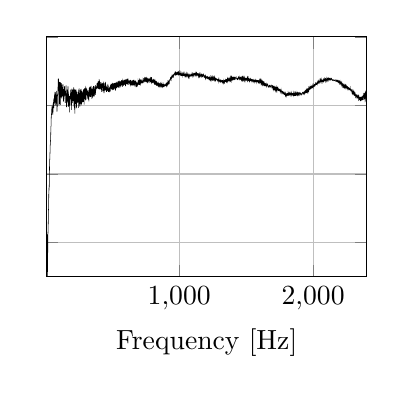
\begin{tikzpicture}

\begin{axis}[%
width=1.6in,
height=1.2in,
at={(1.011in,0.642in)},
scale only axis,
xmin=10,
xmax=2400,
xmajorgrids,
ymin=-10,
ymax=60,
ymajorgrids,
yticklabels={\empty},
xlabel={Frequency [Hz]},
axis background/.style={fill=white}
]
\addplot [color=black,solid,line width=0.2pt,forget plot]
  table[row sep=crcr]{%
0	-0.501897240379707\\
0.666675926054529	9.46126534077405\\
1.33335185210906	18.3601741333859\\
2.00002777816359	-3.15557338844148\\
2.66670370421811	3.42419145357695\\
3.33337963027264	2.3052717079029\\
4.00005555632717	3.78504954020436\\
4.6667314823817	-13.0511251635744\\
5.33340740843623	-3.66370699490856\\
6.00008333449076	-11.4014516722447\\
6.66675926054529	2.61200936043814\\
7.33343518659981	0.462048073848948\\
8.00011111265434	-5.24322004718939\\
8.66678703870887	-10.8621860409649\\
9.3334629647634	-6.16392788613249\\
10.0001388908179	-6.54713271831772\\
10.6668148168725	-6.39432720629177\\
11.333490742927	-10.5817871358799\\
12.0001666689815	-4.9421311662867\\
12.666842595036	-15.6388581411616\\
13.3335185210906	-10.3657729110517\\
14.0001944471451	-13.9822605890021\\
14.6668703731996	-6.02815261124833\\
15.3335462992542	2.41390384195922\\
16.0002222253087	1.07534969299277\\
16.6668981513632	-0.331449890391398\\
17.3335740774177	-8.50584594083159\\
18.0002500034723	-1.02829303709086\\
18.6669259295268	-0.972724417597566\\
19.3336018555813	2.65361582305074\\
20.0002777816359	3.1481352986013\\
20.6669537076904	2.71193617424252\\
21.3336296337449	4.93262806379021\\
22.0003055597994	6.21506391084137\\
22.666981485854	5.93951497202876\\
23.3336574119085	9.41310884290218\\
24.000333337963	9.83859100553316\\
24.6670092640176	11.1891420672423\\
25.3336851900721	13.8320162092132\\
26.0003611161266	14.4280520089158\\
26.6670370421811	12.9898734484199\\
27.3337129682357	15.9813917666039\\
28.0003888942902	15.3917762497441\\
28.6670648203447	15.7297132735923\\
29.3337407463993	16.5992028367615\\
30.0004166724538	18.9507658450566\\
30.6670925985083	20.4610091200905\\
31.3337685245628	22.2286365517974\\
32.0004444506174	23.1486556593599\\
32.6671203766719	24.453154983853\\
33.3337963027264	24.1385698672145\\
34.000472228781	25.2375724709768\\
34.6671481548355	25.9677590140415\\
35.33382408089	26.6498034597212\\
36.0005000069445	27.7198033640538\\
36.6671759329991	28.5479786140492\\
37.3338518590536	28.6355497370829\\
38.0005277851081	29.3024208610392\\
38.6672037111627	29.7057171453665\\
39.3338796372172	30.2053573616138\\
40.0005555632717	31.0561451703245\\
40.6672314893262	32.1944901632832\\
41.3339074153808	32.960618345966\\
42.0005833414353	33.8935062339177\\
42.6672592674898	34.0080334519844\\
43.3339351935444	34.9727909294203\\
44.0006111195989	36.3222029934872\\
44.6672870456534	37.0294949507298\\
45.3339629717079	37.5262865159574\\
46.0006388977625	37.2271572825576\\
46.667314823817	38.2911337376473\\
47.3339907498715	39.0164038181246\\
48.0006666759261	38.7762418282669\\
48.6673426019806	38.5744459560591\\
49.3340185280351	39.2044250846206\\
50.0006944540896	39.7348983930549\\
50.6673703801442	38.6161440448243\\
51.3340463061987	38.7082293560248\\
52.0007222322532	39.3646426717122\\
52.6673981583078	38.2073510712473\\
53.3340740843623	38.2513392740487\\
54.0007500104168	39.7175373630744\\
54.6674259364713	38.825840819052\\
55.3341018625259	37.309136582493\\
56.0007777885804	39.548606741894\\
56.6674537146349	40.2253545935147\\
57.3341296406895	38.041814105578\\
58.000805566744	39.7194898846272\\
58.6674814927985	40.653572349992\\
59.334157418853	39.2112008344364\\
60.0008333449076	40.096184555297\\
60.6675092709621	40.9834197515612\\
61.3341851970166	39.8180229858993\\
62.0008611230712	41.5373442879045\\
62.6675370491257	41.6865910580006\\
63.3342129751802	39.2070640963851\\
64.0008889012347	41.9593908322416\\
64.6675648272893	41.271847967809\\
65.3342407533438	40.2827680442384\\
66.0009166793983	42.1614516902158\\
66.6675926054529	40.5197146230542\\
67.3342685315074	42.5980955232053\\
68.0009444575619	42.5444467334362\\
68.6676203836164	41.4445780255769\\
69.334296309671	43.3827232129673\\
70.0009722357255	42.0830552852971\\
70.66764816178	42.2990966801336\\
71.3343240878346	43.9912200297185\\
72.0010000138891	40.8099967892722\\
72.6676759399436	43.0628208099743\\
73.3343518659981	42.303137078423\\
74.0010277920527	41.8123177110928\\
74.6677037181072	41.6064357857449\\
75.3343796441617	42.1668825869665\\
76.0010555702163	43.4520661436292\\
76.6677314962708	40.1348760267495\\
77.3344074223253	42.5725012508859\\
78.0010833483798	42.0452568129886\\
78.6677592744344	40.5455284604952\\
79.3344352004889	43.8668038788996\\
80.0011111265434	41.2332602895743\\
80.667787052598	43.539455847944\\
81.3344629786525	42.19280085089\\
82.001138904707	44.2849193457178\\
82.6678148307615	42.6431428219097\\
83.3344907568161	43.1047090026832\\
84.0011666828706	41.3055925804323\\
84.6678426089251	41.0098861412209\\
85.3345185349797	40.4780892766323\\
86.0011944610342	38.8799228337918\\
86.6678703870887	38.1866293624345\\
87.3345463131432	38.6513198688698\\
88.0012222391978	38.2457427075552\\
88.6678981652523	39.3602158146788\\
89.3345740913068	40.6185329333737\\
90.0012500173614	41.5103755194883\\
90.6679259434159	42.957707736986\\
91.3346018694704	42.9260078541397\\
92.0012777955249	43.4494925620399\\
92.6679537215795	43.1328589208928\\
93.334629647634	43.8256931277995\\
94.0013055736885	45.4007772588546\\
94.667981499743	44.2180773598414\\
95.3346574257976	47.399054414796\\
96.0013333518521	44.9240052854759\\
96.6680092779066	47.8615895647178\\
97.3346852039612	45.9429781215357\\
98.0013611300157	47.4773479478547\\
98.6680370560702	45.2677803880218\\
99.3347129821248	47.8497247223533\\
100.001388908179	44.9526713580972\\
100.668064834234	45.9365785337475\\
101.334740760288	45.805361680883\\
102.001416686343	40.0133372653086\\
102.668092612397	45.0443686434105\\
103.334768538452	41.95544243909\\
104.001444464506	43.7790989300886\\
104.668120390561	45.0014450847944\\
105.334796316616	43.9518748146494\\
106.00147224267	46.8901297315242\\
106.668148168725	43.168558944998\\
107.334824094779	46.1793608404059\\
108.001500020834	44.9309090871103\\
108.668175946888	40.4364399849188\\
109.334851872943	45.217675095025\\
110.001527798997	43.909119960105\\
110.668203725052	45.0622395085495\\
111.334879651106	46.7736282357385\\
112.001555577161	40.1746639329746\\
112.668231503215	44.7551001522181\\
113.33490742927	45.1531859226577\\
114.001583355324	43.4173710826305\\
114.668259281379	44.7921330345084\\
115.334935207433	44.7283621552527\\
116.001611133488	43.6118930000605\\
116.668287059542	45.332733498807\\
117.334962985597	42.3372487976091\\
118.001638911652	43.5087751178039\\
118.668314837706	46.4792087531176\\
119.334990763761	44.8518340072869\\
120.001666689815	42.4589002703184\\
120.66834261587	44.592675707112\\
121.335018541924	42.8912389196918\\
122.001694467979	43.5775137390154\\
122.668370394033	46.0427883698695\\
123.335046320088	45.774607267154\\
124.001722246142	41.9977504068627\\
124.668398172197	43.291757324914\\
125.335074098251	42.9622381105214\\
126.001750024306	42.5778796244756\\
126.66842595036	43.2074075979104\\
127.335101876415	45.3396477832654\\
128.001777802469	43.4983105771545\\
128.668453728524	43.5204388454017\\
129.335129654579	43.734738835549\\
130.001805580633	44.3993020527215\\
130.668481506688	42.7060464826039\\
131.335157432742	44.3959033690565\\
132.001833358797	46.1194990259802\\
132.668509284851	44.5645612143671\\
133.335185210906	44.478187341691\\
134.00186113696	43.5527857137119\\
134.668537063015	43.9696080995172\\
135.335212989069	41.1608609587057\\
136.001888915124	41.392960992279\\
136.668564841178	42.2785003991066\\
137.335240767233	43.551981390162\\
138.001916693287	43.3071068195703\\
138.668592619342	41.8193194714355\\
139.335268545396	44.7321556239105\\
140.001944471451	44.5105376395655\\
140.668620397506	44.478451514457\\
141.33529632356	44.0066593668681\\
142.001972249615	43.1591242544065\\
142.668648175669	45.6644563941682\\
143.335324101724	45.1278930256561\\
144.002000027778	44.356897699086\\
144.668675953833	44.0212998788855\\
145.335351879887	42.5453894051079\\
146.002027805942	44.424321087088\\
146.668703731996	43.7673709881646\\
147.335379658051	43.444401876399\\
148.002055584105	43.1665347513633\\
148.66873151016	40.7733221304451\\
149.335407436214	43.5138155255498\\
150.002083362269	43.7628515231626\\
150.668759288323	42.9470901031403\\
151.335435214378	44.2133132900495\\
152.002111140433	42.8854705631433\\
152.668787066487	43.2677583750134\\
153.335462992542	44.9772798087513\\
154.002138918596	44.8481828472689\\
154.668814844651	45.8653543195677\\
155.335490770705	45.3717541557845\\
156.00216669676	43.2653589138405\\
156.668842622814	43.0125045744066\\
157.335518548869	40.4844706147849\\
158.002194474923	39.4912699207778\\
158.668870400978	41.0361619892403\\
159.335546327032	42.5803741714127\\
160.002222253087	42.9724673281907\\
160.668898179141	43.5285962212289\\
161.335574105196	42.8419616378948\\
162.00225003125	42.445418428039\\
162.668925957305	44.6334660227252\\
163.335601883359	43.7769675229149\\
164.002277809414	41.2020482414912\\
164.668953735469	41.4671056028151\\
165.335629661523	41.3438330812598\\
166.002305587578	41.6274214544927\\
166.668981513632	43.5653168353649\\
167.335657439687	43.8358659763408\\
168.002333365741	43.4092692171296\\
168.669009291796	43.9697166562419\\
169.33568521785	45.5620167138562\\
170.002361143905	43.1922734240996\\
170.669037069959	39.6560101378331\\
171.335712996014	40.544036670794\\
172.002388922068	43.7312465421409\\
172.669064848123	43.7653281709069\\
173.335740774177	41.7133662420077\\
174.002416700232	40.0043323121742\\
174.669092626286	39.944125756014\\
175.335768552341	41.3461818899357\\
176.002444478396	42.3295543784555\\
176.66912040445	41.8325434031345\\
177.335796330505	40.4035535388654\\
178.002472256559	40.4096751058536\\
178.669148182614	39.9714950483962\\
179.335824108668	41.281617157603\\
180.002500034723	42.710266497598\\
180.669175960777	41.1973716233903\\
181.335851886832	37.9962988289928\\
182.002527812886	41.5981471918668\\
182.669203738941	42.8628124873523\\
183.335879664995	40.3837953393345\\
184.00255559105	40.1199660433088\\
184.669231517104	40.7596636669973\\
185.335907443159	42.2368784032536\\
186.002583369213	42.4085454272028\\
186.669259295268	41.5960646980185\\
187.335935221323	42.2240435908243\\
188.002611147377	43.4703267814708\\
188.669287073432	43.7157155348807\\
189.335962999486	42.9995410422411\\
190.002638925541	44.5888827126371\\
190.669314851595	43.840039324643\\
191.33599077765	43.7249395328987\\
192.002666703704	42.926412859515\\
192.669342629759	42.4952428852985\\
193.336018555813	43.647559582725\\
194.002694481868	40.8482417948248\\
194.669370407922	41.4665151992627\\
195.336046333977	40.9205129266503\\
196.002722260031	38.7203094330807\\
196.669398186086	42.878294320062\\
197.33607411214	43.5925923165799\\
198.002750038195	44.9085257345938\\
198.66942596425	44.4900076651024\\
199.336101890304	43.6917942021084\\
200.002777816359	42.5108841765955\\
200.669453742413	41.2027204546155\\
201.336129668468	40.7902358106384\\
202.002805594522	40.80074034794\\
202.669481520577	42.9556827484068\\
203.336157446631	44.6157272389514\\
204.002833372686	43.6058115795942\\
204.66950929874	44.1552914121529\\
205.336185224795	41.8019189182127\\
206.002861150849	41.3756611253076\\
206.669537076904	42.0441100780567\\
207.336213002958	43.2669156472706\\
208.002888929013	44.5030711732685\\
208.669564855067	44.5095274466715\\
209.336240781122	42.9276599653552\\
210.002916707176	41.2491081896052\\
210.669592633231	41.5415915039899\\
211.336268559286	43.4161315421154\\
212.00294448534	45.2736299995668\\
212.669620411395	43.5128198627527\\
213.336296337449	42.1158940187261\\
214.002972263504	39.7335307193094\\
214.669648189558	42.977908287506\\
215.336324115613	44.2782130886518\\
216.003000041667	44.3260689664658\\
216.669675967722	41.61143983\\
217.336351893776	39.2114563856237\\
218.003027819831	44.0522602337368\\
218.669703745885	43.991055542854\\
219.33637967194	43.7936238122228\\
220.003055597994	37.5980632498722\\
220.669731524049	41.3405249507466\\
221.336407450103	44.6926443802044\\
222.003083376158	42.8558463457976\\
222.669759302213	41.6226546509569\\
223.336435228267	40.5454771587231\\
224.003111154322	43.5811030914612\\
224.669787080376	44.5242744507591\\
225.336463006431	40.4556601183771\\
226.003138932485	41.6541863966633\\
226.66981485854	43.6018023124339\\
227.336490784594	44.207090558958\\
228.003166710649	40.9591382617661\\
228.669842636703	41.5252099796425\\
229.336518562758	44.5944150942566\\
230.003194488812	42.6880155603302\\
230.669870414867	39.1523051700968\\
231.336546340921	43.0312229484008\\
232.003222266976	44.0988984324974\\
232.66989819303	39.5459148164815\\
233.336574119085	41.2081439785618\\
234.00325004514	43.9757680749811\\
234.669925971194	41.3437584792719\\
235.336601897249	40.640895573858\\
236.003277823303	43.2907356896778\\
236.669953749358	42.6488451344478\\
237.336629675412	41.2488438614969\\
238.003305601467	43.2235098449589\\
238.669981527521	41.8785406389853\\
239.336657453576	41.7836051678949\\
240.00333337963	42.7714025151466\\
240.670009305685	43.1713478564228\\
241.336685231739	40.8559007215897\\
242.003361157794	42.5527732295061\\
242.670037083848	42.4123412332676\\
243.336713009903	41.2186881735041\\
244.003388935957	43.9856621134727\\
244.670064862012	42.2564938417095\\
245.336740788066	40.9146705066312\\
246.003416714121	43.9977635172684\\
246.670092640176	40.8995032287493\\
247.33676856623	43.2021831511687\\
248.003444492285	43.2861157657156\\
248.670120418339	39.3241908013569\\
249.336796344394	44.6237989489598\\
250.003472270448	40.3983951402709\\
250.670148196503	43.9558218639915\\
251.336824122557	43.0694735090692\\
252.003500048612	41.4670945446622\\
252.670175974666	44.9476323533098\\
253.336851900721	40.5551359302687\\
254.003527826775	44.4757461106316\\
254.67020375283	42.2673418866467\\
255.336879678884	42.365954118042\\
256.003555604939	43.3334903828934\\
256.670231530993	39.8427418806152\\
257.336907457048	43.5652216008467\\
258.003583383103	39.6485667693289\\
258.670259309157	43.2834997414473\\
259.336935235212	42.1015346989856\\
260.003611161266	43.2590937454771\\
260.670287087321	43.2067331081835\\
261.336963013375	43.4662719803797\\
262.00363893943	44.4188427772715\\
262.670314865484	42.114348942456\\
263.336990791539	44.7163967454051\\
264.003666717593	40.5202923502765\\
264.670342643648	44.0750501064464\\
265.337018569702	40.3987472724447\\
266.003694495757	43.2313157014979\\
266.670370421811	40.0381794452236\\
267.337046347866	44.8403240831374\\
268.00372227392	40.4761286856733\\
268.670398199975	44.2672167828718\\
269.33707412603	41.510297330904\\
270.003750052084	43.6523478369985\\
270.670425978139	40.4157157297354\\
271.337101904193	43.996720916562\\
272.003777830248	41.2329236903023\\
272.670453756302	43.293850165816\\
273.337129682357	42.5284563883139\\
274.003805608411	44.2458699917984\\
274.670481534466	42.1633135166373\\
275.33715746052	41.8811266581356\\
276.003833386575	42.608210887208\\
276.670509312629	40.8992039248973\\
277.337185238684	42.6138998525341\\
278.003861164738	41.6845132166903\\
278.670537090793	43.845908133565\\
279.337213016847	42.2640873888032\\
280.003888942902	41.7988649266827\\
280.670564868956	43.0967421205686\\
281.337240795011	42.6783189390662\\
282.003916721066	43.7497743257782\\
282.67059264712	41.2255076828387\\
283.337268573175	41.0216512716335\\
284.003944499229	43.3019787383773\\
284.670620425284	42.7634639531751\\
285.337296351338	44.7723246868777\\
286.003972277393	42.4611224087962\\
286.670648203447	41.6198858148926\\
287.337324129502	43.6199248400898\\
288.004000055556	42.8698430995207\\
288.670675981611	43.176313225697\\
289.337351907665	42.5207912288017\\
290.00402783372	40.2321276517492\\
290.670703759774	43.3872445666311\\
291.337379685829	44.969437760769\\
292.004055611883	43.1251621871407\\
292.670731537938	42.2922325771393\\
293.337407463993	42.2160689089433\\
294.004083390047	42.5840455782383\\
294.670759316102	43.6542491365296\\
295.337435242156	44.9470751224709\\
296.004111168211	43.8014363458134\\
296.670787094265	42.1767206092466\\
297.33746302032	43.8777316259932\\
298.004138946374	44.1763787819258\\
298.670814872429	41.4715532123527\\
299.337490798483	42.2026330736166\\
300.004166724538	44.8704418746936\\
300.670842650592	44.9996477893037\\
301.337518576647	42.9080634216618\\
302.004194502701	43.1642821178119\\
302.670870428756	44.7991792262513\\
303.33754635481	43.3259042685535\\
304.004222280865	41.7264765015026\\
304.67089820692	42.5921891555734\\
305.337574132974	43.7160157451793\\
306.004250059029	43.7721982950545\\
306.670925985083	43.4993536596701\\
307.337601911138	44.0475061307738\\
308.004277837192	43.3097604617218\\
308.670953763247	43.2654474192193\\
309.337629689301	44.8136008688919\\
310.004305615356	44.7486729745687\\
310.67098154141	43.0195238621092\\
311.337657467465	43.387725799641\\
312.004333393519	44.0255570237817\\
312.671009319574	43.2512795138968\\
313.337685245628	43.5883850769745\\
314.004361171683	44.2634203275993\\
314.671037097737	43.9392540537273\\
315.337713023792	41.9856721910107\\
316.004388949847	43.0444802031941\\
316.671064875901	42.898021745087\\
317.337740801956	43.0619447949383\\
318.00441672801	43.7642351757345\\
318.671092654065	44.3962839207441\\
319.337768580119	43.4912292732289\\
320.004444506174	44.0479024812667\\
320.671120432228	43.7063160497591\\
321.337796358283	41.692919747476\\
322.004472284337	43.5283466667036\\
322.671148210392	43.3911140650906\\
323.337824136446	42.3134422141672\\
324.004500062501	43.5629582561728\\
324.671175988555	41.2146484500885\\
325.33785191461	42.2209695828914\\
326.004527840664	43.1601609778181\\
326.671203766719	44.102693061524\\
327.337879692774	44.0746536743168\\
328.004555618828	45.0497419969146\\
328.671231544883	43.5481290054361\\
329.337907470937	45.4018587103545\\
330.004583396992	44.7869054464032\\
330.671259323046	44.1956100718215\\
331.337935249101	44.1562154181892\\
332.004611175155	42.4925229778274\\
332.67128710121	43.7926397508745\\
333.337963027264	43.0233899281842\\
334.004638953319	42.4386246850847\\
334.671314879373	43.0350617954633\\
335.337990805428	43.7450321731394\\
336.004666731482	45.3992020637462\\
336.671342657537	44.2068607697583\\
337.338018583591	44.3253840896941\\
338.004694509646	44.6068266489781\\
338.671370435701	43.1624845335162\\
339.338046361755	43.2779981033962\\
340.00472228781	42.5119263742027\\
340.671398213864	44.9861388698404\\
341.338074139919	45.680423588641\\
342.004750065973	43.5920906309355\\
342.671425992028	44.788250663947\\
343.338101918082	43.1389549229424\\
344.004777844137	43.1474783103432\\
344.671453770191	43.276491894657\\
345.338129696246	44.6360425873325\\
346.0048056223	44.527160427757\\
346.671481548355	42.9363196920201\\
347.338157474409	43.6693058601854\\
348.004833400464	41.9192151707457\\
348.671509326518	44.0955970059269\\
349.338185252573	44.5242722528314\\
350.004861178627	44.4874360935875\\
350.671537104682	42.2490301770806\\
351.338213030737	44.1210204337576\\
352.004888956791	44.0000930987503\\
352.671564882846	44.9044970021603\\
353.3382408089	44.5006495817104\\
354.004916734955	42.9167905281371\\
354.671592661009	43.6354277368127\\
355.338268587064	44.8434275991471\\
356.004944513118	44.7637636648996\\
356.671620439173	43.934991016836\\
357.338296365227	42.5733023602905\\
358.004972291282	45.3089793294824\\
358.671648217336	45.6740134271839\\
359.338324143391	42.698443034845\\
360.005000069445	44.0303454700881\\
360.6716759955	44.4620323324116\\
361.338351921554	45.1094324741305\\
362.005027847609	43.3828744523386\\
362.671703773664	43.8668558614971\\
363.338379699718	45.6105392237094\\
364.005055625773	42.8825767693103\\
364.671731551827	44.0061600458498\\
365.338407477882	42.7577963085769\\
366.005083403936	44.7070768477394\\
366.671759329991	42.672617832381\\
367.338435256045	44.8532125094446\\
368.0051111821	43.4498467840792\\
368.671787108154	43.6100548151763\\
369.338463034209	44.1795954389944\\
370.005138960263	44.4904179522328\\
370.671814886318	43.775505482871\\
371.338490812372	43.8763795844873\\
372.005166738427	45.3699032922028\\
372.671842664481	43.523051021927\\
373.338518590536	45.9351362723457\\
374.005194516591	43.0667959219461\\
374.671870442645	45.3688964990518\\
375.3385463687	43.6351871092132\\
376.005222294754	45.026746404214\\
376.671898220809	44.3419164403517\\
377.338574146863	44.9874375027727\\
378.005250072918	44.7001478399489\\
378.671925998972	44.7650694886119\\
379.338601925027	45.4929723280979\\
380.005277851081	45.0199651796302\\
380.671953777136	45.5693470181451\\
381.33862970319	44.8416117031851\\
382.005305629245	45.0436981867725\\
382.671981555299	45.1732697693337\\
383.338657481354	45.2629842255761\\
384.005333407408	45.2561847835062\\
384.672009333463	46.2309507272709\\
385.338685259517	44.9119220612911\\
386.005361185572	46.4180050250669\\
386.672037111627	45.4194587911707\\
387.338713037681	45.4178045603765\\
388.005388963736	46.5256690609214\\
388.67206488979	45.987724003035\\
389.338740815845	46.1016829060332\\
390.005416741899	46.4164586434507\\
390.672092667954	45.0539919170534\\
391.338768594008	46.3758081685014\\
392.005444520063	45.6699469097933\\
392.672120446117	45.8431317816176\\
393.338796372172	46.9301912808021\\
394.005472298226	44.7988092011732\\
394.672148224281	45.4681602833131\\
395.338824150335	46.4580332843074\\
396.00550007639	45.3313624572723\\
396.672176002444	46.2981756676233\\
397.338851928499	45.926340111236\\
398.005527854554	44.8765333151579\\
398.672203780608	46.8621116128483\\
399.338879706663	46.8229091398723\\
400.005555632717	45.1893644753673\\
400.672231558772	45.8178458485993\\
401.338907484826	47.6812541074286\\
402.005583410881	44.9574262095323\\
402.672259336935	46.3470300643472\\
403.33893526299	46.4848702245909\\
404.005611189044	44.7013671982634\\
404.672287115099	45.1142224985818\\
405.338963041153	47.135509186731\\
406.005638967208	46.1779483122175\\
406.672314893262	44.982391075966\\
407.338990819317	45.6867667724594\\
408.005666745371	46.8287535384239\\
408.672342671426	45.9368179928359\\
409.339018597481	44.7850970464569\\
410.005694523535	46.8118819627215\\
410.67237044959	46.3331437238239\\
411.339046375644	45.0826086171263\\
412.005722301699	45.3871365732788\\
412.672398227753	46.0686422470052\\
413.339074153808	45.4557064048667\\
414.005750079862	45.3142157483885\\
414.672426005917	45.9936580871129\\
415.339101931971	46.2543028857257\\
416.005777858026	45.751797997296\\
416.67245378408	46.0149354628953\\
417.339129710135	45.3070869649923\\
418.005805636189	44.8240014396089\\
418.672481562244	44.8674366805609\\
419.339157488298	45.8736345481349\\
420.005833414353	46.6296288213359\\
420.672509340407	45.5126380217137\\
421.339185266462	43.951520081948\\
422.005861192517	45.0356649472724\\
422.672537118571	46.1179590888196\\
423.339213044626	46.4418122510002\\
424.00588897068	46.2073003762281\\
424.672564896735	45.2858083844029\\
425.339240822789	45.357013621376\\
426.005916748844	45.9860928175329\\
426.672592674898	45.9143648178613\\
427.339268600953	45.8772495113727\\
428.005944527007	45.9641647847651\\
428.672620453062	46.2983603486093\\
429.339296379116	46.2308765335601\\
430.005972305171	45.0107450824477\\
430.672648231225	44.2156492484632\\
431.33932415728	44.4185038432861\\
432.006000083334	45.2476857068552\\
432.672676009389	46.4654082278003\\
433.339351935444	46.5445736504842\\
434.006027861498	45.3187464456428\\
434.672703787553	45.5769635970127\\
435.339379713607	46.4155161538099\\
436.006055639662	45.7456135156555\\
436.672731565716	45.2899547633244\\
437.339407491771	44.7932819699026\\
438.006083417825	43.6333998488684\\
438.67275934388	43.9357163115821\\
439.339435269934	44.2920097002549\\
440.006111195989	45.1428995869021\\
440.672787122043	45.1509929873562\\
441.339463048098	44.1876240062728\\
442.006138974152	44.6052674362121\\
442.672814900207	44.7949283868502\\
443.339490826261	46.0840254308058\\
444.006166752316	46.3553528948909\\
444.672842678371	46.5642132410983\\
445.339518604425	46.2119773902423\\
446.00619453048	46.2250283564056\\
446.672870456534	45.4984386458887\\
447.339546382589	45.4261609759142\\
448.006222308643	44.5132678100075\\
448.672898234698	45.2867795139739\\
449.339574160752	45.7485785021503\\
450.006250086807	46.8886565868429\\
450.672926012861	46.3832488359576\\
451.339601938916	45.8534503863317\\
452.00627786497	44.7849640987676\\
452.672953791025	44.2779445845579\\
453.339629717079	44.5785531143514\\
454.006305643134	44.7702978534214\\
454.672981569188	45.3195031368541\\
455.339657495243	44.9538323463271\\
456.006333421298	45.0624838046577\\
456.673009347352	43.9851899331527\\
457.339685273407	44.8249025674395\\
458.006361199461	45.302964222391\\
458.673037125516	45.2586004335258\\
459.33971305157	44.8715707817385\\
460.006388977625	44.8354421685582\\
460.673064903679	44.6447342098071\\
461.339740829734	44.6846899305244\\
462.006416755788	44.7958003025342\\
462.673092681843	44.248758250556\\
463.339768607897	44.4312230379635\\
464.006444533952	44.1881724460186\\
464.673120460006	45.6908666937175\\
465.339796386061	45.7814911731749\\
466.006472312115	45.3600075972798\\
466.67314823817	46.2683159927871\\
467.339824164225	45.2388702587511\\
468.006500090279	45.359667740547\\
468.673176016334	44.8991164116883\\
469.339851942388	44.3079920120319\\
470.006527868443	45.7645252404021\\
470.673203794497	45.1172716384468\\
471.339879720552	43.9563438246388\\
472.006555646606	44.6988213235873\\
472.673231572661	44.3654287939518\\
473.339907498715	43.9980638582965\\
474.00658342477	44.6573084044057\\
474.673259350824	44.9772806502009\\
475.339935276879	44.5090005795042\\
476.006611202933	43.8191160595859\\
476.673287128988	44.9091910624805\\
477.339963055042	44.2092189169214\\
478.006638981097	44.2464006912178\\
478.673314907152	45.2428930009038\\
479.339990833206	44.0266662609489\\
480.006666759261	44.2711221692355\\
480.673342685315	44.908042839383\\
481.34001861137	44.0705169672244\\
482.006694537424	44.4666845279605\\
482.673370463479	44.7465787810396\\
483.340046389533	44.0140859222645\\
484.006722315588	45.60495203064\\
484.673398241642	44.7646455022048\\
485.340074167697	44.2036371096453\\
486.006750093751	45.8434906335666\\
486.673426019806	45.3351202344568\\
487.34010194586	45.8071009991448\\
488.006777871915	45.3984766128266\\
488.673453797969	45.9174779973642\\
489.340129724024	46.2626198199461\\
490.006805650078	44.9280627082302\\
490.673481576133	46.2223881539612\\
491.340157502188	45.7102502454284\\
492.006833428242	45.3565030082699\\
492.673509354297	45.4868467311448\\
493.340185280351	44.6780541077425\\
494.006861206406	45.686438571504\\
494.67353713246	45.3129149110806\\
495.340213058515	45.2286164783783\\
496.006888984569	45.2080397786882\\
496.673564910624	45.674249027754\\
497.340240836678	44.6992830096064\\
498.006916762733	46.246818137008\\
498.673592688787	44.9040486176897\\
499.340268614842	46.5908567261213\\
500.006944540896	45.912911316527\\
500.673620466951	46.0853001284064\\
501.340296393005	45.8870139985496\\
502.00697231906	45.2442142200493\\
502.673648245115	45.0473236170449\\
503.340324171169	44.5098716056778\\
504.007000097224	45.1850465668928\\
504.673676023278	45.2964894105685\\
505.340351949333	45.5421591467752\\
506.007027875387	46.466855374144\\
506.673703801442	45.3766064397913\\
507.340379727496	46.1306519142724\\
508.007055653551	44.5855345032381\\
508.673731579605	46.1535006117522\\
509.34040750566	44.6026305523417\\
510.007083431714	46.2880170652069\\
510.673759357769	45.518433526499\\
511.340435283823	46.0822142831911\\
512.007111209878	46.4171790895978\\
512.673787135932	44.8319674595096\\
513.340463061987	45.7224007266426\\
514.007138988041	45.1379936907807\\
514.673814914096	45.8554891392455\\
515.340490840151	46.1147147761718\\
516.007166766205	46.5423481103261\\
516.67384269226	46.1020499650716\\
517.340518618314	45.078964678522\\
518.007194544369	45.5414285112879\\
518.673870470423	45.8156383925924\\
519.340546396478	45.0258394978104\\
520.007222322532	46.5931200385472\\
520.673898248587	46.3471611350183\\
521.340574174641	44.4490878420333\\
522.007250100696	45.8916308145559\\
522.67392602675	45.5596093880293\\
523.340601952805	46.551191175224\\
524.007277878859	46.3632304783785\\
524.673953804914	44.3565334621307\\
525.340629730968	45.3959724965016\\
526.007305657023	46.4667513993333\\
526.673981583078	45.286370568925\\
527.340657509132	46.5456107398885\\
528.007333435187	46.1479406133293\\
528.674009361241	44.9227514481399\\
529.340685287296	46.141126802986\\
530.00736121335	46.9050839637573\\
530.674037139405	45.3610471946591\\
531.340713065459	45.1438152937687\\
532.007388991514	46.1774081313653\\
532.674064917568	46.3937706227979\\
533.340740843623	46.3162953893224\\
534.007416769677	46.0006424651687\\
534.674092695732	46.2610455048393\\
535.340768621786	46.2811217328832\\
536.007444547841	46.0973951591228\\
536.674120473896	45.9544374054796\\
537.34079639995	46.2568213814647\\
538.007472326005	46.3686949952295\\
538.674148252059	45.7747878566089\\
539.340824178114	45.6890190597599\\
540.007500104168	46.1409531110252\\
540.674176030223	46.6073601218127\\
541.340851956277	45.8653871486027\\
542.007527882332	45.3893341563742\\
542.674203808386	45.9844713648959\\
543.340879734441	47.0057644739524\\
544.007555660495	46.7137363857969\\
544.67423158655	45.1705322266592\\
545.340907512604	46.309833190284\\
546.007583438659	47.1909634622888\\
546.674259364713	46.2791183333291\\
547.340935290768	46.1484933507798\\
548.007611216823	46.3417201758744\\
548.674287142877	45.838287671593\\
549.340963068932	45.2777602201429\\
550.007638994986	46.4060470404105\\
550.674314921041	46.5616919010915\\
551.340990847095	45.9364237966108\\
552.00766677315	45.7317835505511\\
552.674342699204	46.1302071302985\\
553.341018625259	45.6683243149358\\
554.007694551313	45.7827590780553\\
554.674370477368	46.6623217441592\\
555.341046403422	46.5011584678333\\
556.007722329477	46.6048990413136\\
556.674398255531	47.0480581806329\\
557.341074181586	46.4499303755301\\
558.00775010764	46.0439647320717\\
558.674426033695	46.9182754136817\\
559.341101959749	45.907901057103\\
560.007777885804	45.8563338971789\\
560.674453811858	46.4315069698922\\
561.341129737913	45.7645261838897\\
562.007805663968	45.8861116962115\\
562.674481590022	46.7032093460544\\
563.341157516077	46.3455912038482\\
564.007833442131	46.8709721236774\\
564.674509368186	47.0761729692437\\
565.34118529424	45.991149605742\\
566.007861220295	46.847420723664\\
566.674537146349	46.3987396194371\\
567.341213072404	46.5965764411098\\
568.007888998458	47.3757597115367\\
568.674564924513	47.1560251395102\\
569.341240850567	46.8557504804509\\
570.007916776622	47.1153668972031\\
570.674592702676	45.8386796930997\\
571.341268628731	46.8582927385801\\
572.007944554785	46.3014007332838\\
572.67462048084	46.4513883650974\\
573.341296406895	46.6939150110147\\
574.007972332949	46.2080650477376\\
574.674648259004	47.2985029244536\\
575.341324185058	47.1823914845687\\
576.008000111113	46.6989794634984\\
576.674676037167	46.5267970215412\\
577.341351963222	45.4192935613471\\
578.008027889276	46.8273203886267\\
578.674703815331	46.6174509345774\\
579.341379741385	46.9668411093232\\
580.00805566744	46.4090808167623\\
580.674731593494	46.3111432056171\\
581.341407519549	47.2369916832945\\
582.008083445603	45.6807256663379\\
582.674759371658	47.0196725509517\\
583.341435297712	46.714244310203\\
584.008111223767	46.893434792227\\
584.674787149822	46.3620269840306\\
585.341463075876	46.1360960355697\\
586.008139001931	46.9745429188527\\
586.674814927985	47.0674197775891\\
587.34149085404	47.4357775658722\\
588.008166780094	46.004430420175\\
588.674842706149	46.6702036991167\\
589.341518632203	46.1567456585399\\
590.008194558258	47.4764910471885\\
590.674870484312	46.5785076894449\\
591.341546410367	46.5261755624496\\
592.008222336421	46.6857178802229\\
592.674898262476	46.8901075017408\\
593.34157418853	46.0980058133264\\
594.008250114585	47.0271332970476\\
594.674926040639	47.133600461865\\
595.341601966694	46.6845467761701\\
596.008277892749	46.5037137927752\\
596.674953818803	46.3875847819321\\
597.341629744858	47.1525979203549\\
598.008305670912	47.4226612621204\\
598.674981596967	45.6669538295091\\
599.341657523021	46.9913574973429\\
600.008333449076	47.5412054939054\\
600.67500937513	45.9540383589003\\
601.341685301185	46.763708794061\\
602.008361227239	47.0714840457704\\
602.675037153294	46.4576420853782\\
603.341713079348	47.0469061900243\\
604.008389005403	46.3064766559505\\
604.675064931457	47.5839880811663\\
605.341740857512	46.456336148386\\
606.008416783566	47.2237898766917\\
606.675092709621	46.334568131365\\
607.341768635676	47.5669062913329\\
608.00844456173	46.7955373297399\\
608.675120487785	46.7021637410332\\
609.341796413839	47.4836186859527\\
610.008472339894	46.5254478331813\\
610.675148265948	47.1848448043186\\
611.341824192003	47.0564004586199\\
612.008500118057	46.5047476450475\\
612.675176044112	46.7092454594831\\
613.341851970166	47.6922664558082\\
614.008527896221	46.2145574587238\\
614.675203822275	47.7940599101367\\
615.34187974833	46.4614546373285\\
616.008555674384	46.9153020367259\\
616.675231600439	47.2958717736041\\
617.341907526493	46.1057216858172\\
618.008583452548	47.818412066672\\
618.675259378603	46.2617124617528\\
619.341935304657	47.2979730461596\\
620.008611230711	47.0672277363301\\
620.675287156766	46.7693789973899\\
621.341963082821	47.2439987488194\\
622.008639008875	46.5595484036455\\
622.67531493493	47.1959148395154\\
623.341990860984	46.8754236422635\\
624.008666787039	46.8976757210031\\
624.675342713093	47.1082985973579\\
625.342018639148	46.678323938622\\
626.008694565202	46.8140114029384\\
626.675370491257	46.7673877324648\\
627.342046417311	46.6819791732888\\
628.008722343366	46.7590500004966\\
628.67539826942	46.9326622849338\\
629.342074195475	46.3505390898222\\
630.008750121529	46.8192474355273\\
630.675426047584	46.7203941698994\\
631.342101973638	46.6688794738765\\
632.008777899693	46.4709538888141\\
632.675453825748	47.2432565530704\\
633.342129751802	45.8959874715655\\
634.008805677857	47.3617357406798\\
634.675481603911	46.4362794000502\\
635.342157529966	46.273652947751\\
636.00883345602	46.8841613909476\\
636.675509382075	46.3706021393771\\
637.342185308129	46.3731599290267\\
638.008861234184	46.1970819695477\\
638.675537160238	46.9208329865482\\
639.342213086293	45.9661331347473\\
640.008889012347	47.0116997501538\\
640.675564938402	46.901207546934\\
641.342240864456	45.9985327612917\\
642.008916790511	46.6636249676676\\
642.675592716565	46.5170210150195\\
643.34226864262	46.3734743932579\\
644.008944568675	46.8202138620222\\
644.675620494729	46.2329833330021\\
645.342296420784	46.7905001553905\\
646.008972346838	46.7058858854156\\
646.675648272893	45.9645923896903\\
647.342324198947	46.4800773660099\\
648.009000125002	46.9219655684095\\
648.675676051056	46.4227105482025\\
649.342351977111	46.5645386733707\\
650.009027903165	46.7088724119949\\
650.67570382922	46.9236767629877\\
651.342379755274	46.8154196507466\\
652.009055681329	45.9060612704215\\
652.675731607383	46.2750044083199\\
653.342407533438	47.4011177450831\\
654.009083459492	46.9970370551623\\
654.675759385547	45.8695179234236\\
655.342435311602	46.1537168510962\\
656.009111237656	47.0334818429577\\
656.675787163711	46.9953333786586\\
657.342463089765	46.4945774562971\\
658.00913901582	46.627053121622\\
658.675814941874	46.8192771984754\\
659.342490867929	46.5142571782078\\
660.009166793983	46.3896695333732\\
660.675842720038	46.9443904650335\\
661.342518646092	47.5234174116647\\
662.009194572147	46.8614521448938\\
662.675870498201	45.9034133353399\\
663.342546424256	46.2111823436178\\
664.00922235031	46.7069373316567\\
664.675898276365	47.0450851873258\\
665.342574202419	47.0637980865803\\
666.009250128474	46.4259697351722\\
666.675926054529	46.24297764224\\
667.342601980583	46.5855870882685\\
668.009277906638	46.421543124005\\
668.675953832692	46.1363405446746\\
669.342629758747	46.022585536393\\
670.009305684801	46.516166828173\\
670.675981610856	47.1394652970405\\
671.34265753691	47.1508000456959\\
672.009333462965	47.0249881900698\\
672.676009389019	46.923567711794\\
673.342685315074	46.8221087857817\\
674.009361241128	46.8893239331826\\
674.676037167183	46.6387850939104\\
675.342713093237	46.3256562612641\\
676.009389019292	45.9873377651278\\
676.676064945346	45.8424558660377\\
677.342740871401	46.1416652533965\\
678.009416797456	46.6237024666016\\
678.67609272351	46.5066275772438\\
679.342768649565	46.3584037002231\\
680.009444575619	45.6900253438025\\
680.676120501674	45.6273846636488\\
681.342796427728	45.6027753655371\\
682.009472353783	46.2554492515993\\
682.676148279837	46.3987927668185\\
683.342824205892	46.4725776036248\\
684.009500131946	45.9515988973665\\
684.676176058001	45.675299327646\\
685.342851984055	45.6316806422499\\
686.00952791011	45.8234203480471\\
686.676203836164	46.0502713041155\\
687.342879762219	46.3614493923659\\
688.009555688273	46.3396347927259\\
688.676231614328	46.1023013338999\\
689.342907540382	46.0071505449831\\
690.009583466437	46.0872753728266\\
690.676259392492	46.1265251538189\\
691.342935318546	46.6187134654212\\
692.009611244601	46.6918136963872\\
692.676287170655	47.1418866651912\\
693.34296309671	46.9786814749525\\
694.009639022764	47.3169194900422\\
694.676314948819	46.7402812539153\\
695.342990874873	46.7200373482746\\
696.009666800928	46.5568948797893\\
696.676342726982	46.3471234588622\\
697.343018653037	46.2873642323989\\
698.009694579091	46.0411263814803\\
698.676370505146	46.5786029520192\\
699.3430464312	47.0936041133584\\
700.009722357255	47.0399879779027\\
700.676398283309	46.6954085946834\\
701.343074209364	46.4677667364552\\
702.009750135419	46.6294579106411\\
702.676426061473	47.1560636977367\\
703.343101987528	47.4296050124375\\
704.009777913582	47.5415184218619\\
704.676453839637	47.2601721955097\\
705.343129765691	46.6860339055224\\
706.009805691746	46.291724499283\\
706.6764816178	45.9835211253975\\
707.343157543855	46.5234274313943\\
708.009833469909	47.5866365949543\\
708.676509395964	47.1696179998539\\
709.343185322018	45.8290897558937\\
710.009861248073	46.1596419626102\\
710.676537174127	46.7743496353779\\
711.343213100182	47.0569922204346\\
712.009889026236	47.1099442558402\\
712.676564952291	46.7929230404258\\
713.343240878346	46.3651874886468\\
714.0099168044	46.8057120058967\\
714.676592730455	47.4999440271867\\
715.343268656509	47.2007212249569\\
716.009944582564	46.3861386364413\\
716.676620508618	46.9519992707991\\
717.343296434673	47.5189334552868\\
718.009972360727	46.7510653768242\\
718.676648286782	47.0189573190302\\
719.343324212836	46.8787822487504\\
720.010000138891	46.9255624472996\\
720.676676064945	47.2274753837696\\
721.343351991	46.6407819281331\\
722.010027917054	46.9400429106056\\
722.676703843109	46.8919824781839\\
723.343379769163	46.6184125953048\\
724.010055695218	47.062097881945\\
724.676731621273	47.0626067727442\\
725.343407547327	46.4230564329149\\
726.010083473382	47.1342368711811\\
726.676759399436	46.7961625878438\\
727.343435325491	47.048127608479\\
728.010111251545	47.3719067519032\\
728.6767871776	46.9661402926055\\
729.343463103654	47.4390246438457\\
730.010139029709	47.2709714345613\\
730.676814955763	47.9040312780523\\
731.343490881818	47.1703958097387\\
732.010166807872	47.9512917525358\\
732.676842733927	47.2043979545296\\
733.343518659981	47.4259418808982\\
734.010194586036	47.4048700171379\\
734.67687051209	46.6308573568309\\
735.343546438145	47.4685079870876\\
736.0102223642	46.5346116010819\\
736.676898290254	47.177025079223\\
737.343574216309	46.9062792180229\\
738.010250142363	47.2315204367465\\
738.676926068418	47.2330943031754\\
739.343601994472	47.6101987990534\\
740.010277920527	47.4821272117845\\
740.676953846581	47.6676416243217\\
741.343629772636	47.3340903261707\\
742.01030569869	47.3431682933545\\
742.676981624745	46.9734140182743\\
743.343657550799	47.3834594959475\\
744.010333476854	46.9796799108305\\
744.677009402908	47.6993752980141\\
745.343685328963	47.4334976856789\\
746.010361255017	47.7143318055892\\
746.677037181072	47.6060809868436\\
747.343713107127	47.3433933501318\\
748.010389033181	47.493999371971\\
748.677064959236	46.9883128695617\\
749.34374088529	47.2006109637042\\
750.010416811345	47.7463714861302\\
750.677092737399	47.2578005067674\\
751.343768663454	48.274154810652\\
752.010444589508	47.2353805270321\\
752.677120515563	47.4088719300324\\
753.343796441617	47.1248801884225\\
754.010472367672	47.2128223071475\\
754.677148293726	47.4343545914519\\
755.343824219781	47.5224295942296\\
756.010500145835	47.692236182077\\
756.67717607189	47.2251656575916\\
757.343851997944	46.9178112403977\\
758.010527923999	47.3581711830166\\
758.677203850054	47.7289368578666\\
759.343879776108	47.3311522580687\\
760.010555702162	48.1093926573779\\
760.677231628217	47.4860520918866\\
761.343907554272	46.5405590101866\\
762.010583480326	47.8742293596583\\
762.677259406381	47.5372466396233\\
763.343935332435	47.3284522513077\\
764.01061125849	47.6956961611049\\
764.677287184544	47.0378891630234\\
765.343963110599	47.1556025079457\\
766.010639036653	47.8662455912647\\
766.677314962708	47.5771363903443\\
767.343990888762	47.3728986554281\\
768.010666814817	47.0708399033557\\
768.677342740871	47.3509859783906\\
769.344018666926	47.7867370533772\\
770.01069459298	47.3603524664898\\
770.677370519035	47.1950132296965\\
771.344046445089	47.4946879908574\\
772.010722371144	47.5474517164677\\
772.677398297199	46.955051014863\\
773.344074223253	47.4031479228311\\
774.010750149308	47.6523457910367\\
774.677426075362	47.5713308091181\\
775.344102001417	47.2478291243165\\
776.010777927471	47.2941358191791\\
776.677453853526	47.4120691210141\\
777.34412977958	47.5165368220259\\
778.010805705635	47.4828047584883\\
778.677481631689	47.3365399261514\\
779.344157557744	47.2966201186484\\
780.010833483798	47.6292561688127\\
780.677509409853	47.5306162213568\\
781.344185335907	46.8431225856916\\
782.010861261962	46.8849816593786\\
782.677537188016	47.7120657771746\\
783.344213114071	47.8315529246182\\
784.010889040126	47.4506441173785\\
784.67756496618	47.6526051341474\\
785.344240892235	47.6845424197461\\
786.010916818289	47.207735286322\\
786.677592744344	46.92188327103\\
787.344268670398	47.5408565633559\\
788.010944596453	47.666871456914\\
788.677620522507	47.2699575634138\\
789.344296448562	47.3193827464526\\
790.010972374616	47.5357383326162\\
790.677648300671	46.7115058540781\\
791.344324226725	46.6391466339422\\
792.01100015278	47.5071906210957\\
792.677676078834	47.4076482046549\\
793.344352004889	47.4196955938159\\
794.011027930943	48.2283679308869\\
794.677703856998	47.7848411500436\\
795.344379783053	47.3535229236034\\
796.011055709107	47.8414985793\\
796.677731635162	47.0861958253498\\
797.344407561216	46.7013223657381\\
798.011083487271	47.045812951041\\
798.677759413325	46.6607616203084\\
799.34443533938	46.6510676914334\\
800.011111265434	47.1766087294334\\
800.677787191489	47.0886810363081\\
801.344463117543	47.0566390385801\\
802.011139043598	47.4793314548395\\
802.677814969652	46.9749224880463\\
803.344490895707	46.9727929718354\\
804.011166821761	47.339985955171\\
804.677842747816	46.6872985721067\\
805.34451867387	47.2613981007464\\
806.011194599925	47.3078478010528\\
806.67787052598	47.12707337035\\
807.344546452034	47.7821558638155\\
808.011222378089	47.3070458698611\\
808.677898304143	47.2764567870693\\
809.344574230198	47.4346813939923\\
810.011250156252	46.5943687639227\\
810.677926082307	47.1144846071876\\
811.344602008361	46.5805145233973\\
812.011277934416	46.4969440332802\\
812.67795386047	46.8523280863109\\
813.344629786525	46.6443785956032\\
814.011305712579	47.233860218705\\
814.677981638634	47.2024683337716\\
815.344657564688	46.6662585199825\\
816.011333490743	46.6859635789227\\
816.678009416797	46.0643364334579\\
817.344685342852	46.9760032938154\\
818.011361268907	46.848282467613\\
818.678037194961	47.039752077336\\
819.344713121016	46.7151650380437\\
820.01138904707	46.1087903164503\\
820.678064973125	46.5848379676865\\
821.344740899179	46.2893159831474\\
822.011416825234	47.2363904062814\\
822.678092751288	46.5229357956181\\
823.344768677343	46.8799147023029\\
824.011444603397	46.3967903122602\\
824.678120529452	46.199970918561\\
825.344796455506	46.80313194984\\
826.011472381561	46.3778064545798\\
826.678148307615	46.4609815022499\\
827.34482423367	46.2009386582806\\
828.011500159724	47.1735822087309\\
828.678176085779	46.3100714016562\\
829.344852011833	46.1869040442484\\
830.011527937888	45.7633735525572\\
830.678203863943	47.0128600171734\\
831.344879789997	46.4364500591784\\
832.011555716052	46.2025815582215\\
832.678231642106	45.8613432654453\\
833.344907568161	46.5755037894735\\
834.011583494215	46.2395504467766\\
834.67825942027	46.3439813870499\\
835.344935346324	46.2045252716936\\
836.011611272379	46.2553253700087\\
836.678287198433	45.9278301924508\\
837.344963124488	46.3861974812002\\
838.011639050542	46.3951146587662\\
838.678314976597	45.8568624630606\\
839.344990902651	45.8862458500885\\
840.011666828706	46.8736050366596\\
840.67834275476	45.653290873425\\
841.345018680815	46.0328570273788\\
842.01169460687	46.2411524188133\\
842.678370532924	46.356281245375\\
843.345046458979	45.6860544220147\\
844.011722385033	46.5947977789213\\
844.678398311088	45.4664640074893\\
845.345074237142	46.4805542895039\\
846.011750163197	45.8844130890732\\
846.678426089251	46.1959401318403\\
847.345102015306	46.1054168160103\\
848.01177794136	45.844335436911\\
848.678453867415	46.0496622265102\\
849.345129793469	46.1224526110016\\
850.011805719524	45.8794768249075\\
850.678481645578	46.0587888836724\\
851.345157571633	46.0642424656158\\
852.011833497687	45.7229499242367\\
852.678509423742	46.4708690102597\\
853.345185349797	45.4776984817063\\
854.011861275851	46.2276175803079\\
854.678537201906	45.8245658821273\\
855.34521312796	45.8758235730824\\
856.011889054015	46.0612283462753\\
856.678564980069	45.8387234522624\\
857.345240906124	46.0983234932452\\
858.011916832178	46.2307976648756\\
858.678592758233	45.7203357358889\\
859.345268684287	46.4616768314686\\
860.011944610342	45.6172847365269\\
860.678620536396	46.1209569443818\\
861.345296462451	45.9941275286542\\
862.011972388505	45.5964476242155\\
862.67864831456	46.3215242762504\\
863.345324240614	45.3184526328994\\
864.012000166669	46.3314431767113\\
864.678676092724	45.6999026116099\\
865.345352018778	46.0379012546695\\
866.012027944833	45.9123933137277\\
866.678703870887	45.930253021153\\
867.345379796942	45.8272278620478\\
868.012055722996	46.1273632993242\\
868.678731649051	45.8612251413306\\
869.345407575105	46.0072573722067\\
870.01208350116	46.1710420382192\\
870.678759427214	45.6344254798269\\
871.345435353269	46.3465403288935\\
872.012111279323	45.7652153365542\\
872.678787205378	45.8813601695881\\
873.345463131432	46.1755558540194\\
874.012139057487	45.7669881722318\\
874.678814983541	45.8615620584098\\
875.345490909596	45.9482597589472\\
876.012166835651	45.8204112004003\\
876.678842761705	45.5852328860372\\
877.34551868776	45.7456425537817\\
878.012194613814	46.0189273161166\\
878.678870539869	45.3951431367452\\
879.345546465923	46.0050637991416\\
880.012222391978	46.0989002788181\\
880.678898318032	45.5423160491902\\
881.345574244087	46.0672282820837\\
882.012250170141	45.931748977446\\
882.678926096196	45.3495788666632\\
883.34560202225	46.243716095959\\
884.012277948305	45.8298150005483\\
884.678953874359	45.3338039645532\\
885.345629800414	46.1054724017152\\
886.012305726468	46.0992149683062\\
886.678981652523	45.4383934620475\\
887.345657578578	45.7966562629403\\
888.012333504632	46.1689260773063\\
888.679009430687	45.6614846779447\\
889.345685356741	45.661769847818\\
890.012361282796	45.8614377571122\\
890.67903720885	45.9936435406662\\
891.345713134905	45.9686991555235\\
892.012389060959	45.80151964678\\
892.679064987014	45.7883092212216\\
893.345740913068	45.9557352213821\\
894.012416839123	46.0846430394006\\
894.679092765177	46.009413897542\\
895.345768691232	45.8488704059475\\
896.012444617286	45.8694443647115\\
896.679120543341	45.824573069088\\
897.345796469395	45.819660849824\\
898.01247239545	46.0494589990329\\
898.679148321504	46.0943678254436\\
899.345824247559	46.0241385457516\\
900.012500173613	45.9103331285116\\
900.679176099668	45.9665150180527\\
901.345852025723	46.1849101722879\\
902.012527951777	46.1226297900694\\
902.679203877832	45.8853444138843\\
903.345879803886	45.9763134302331\\
904.012555729941	46.1919516750006\\
904.679231655995	45.9582847427187\\
905.34590758205	45.7888426641325\\
906.012583508104	45.9753965726312\\
906.679259434159	46.2656793552703\\
907.345935360213	46.3719720423657\\
908.012611286268	46.4045546320674\\
908.679287212322	46.0964146870599\\
909.345963138377	45.8971659294386\\
910.012639064431	46.3496987933111\\
910.679314990486	46.6349486362381\\
911.34599091654	46.4258105711658\\
912.012666842595	46.2483968778973\\
912.67934276865	45.9698422722526\\
913.346018694704	46.0784648551263\\
914.012694620759	46.4982540910758\\
914.679370546813	46.5600097091532\\
915.346046472868	46.5240791602634\\
916.012722398922	46.2301887938844\\
916.679398324977	46.2493814073694\\
917.346074251031	46.4757502465103\\
918.012750177086	46.7265818035177\\
918.67942610314	46.8767161119606\\
919.346102029195	46.7633633052008\\
920.012777955249	46.5916283126179\\
920.679453881304	46.4531567507754\\
921.346129807358	46.627491781375\\
922.012805733413	46.8571009085176\\
922.679481659467	47.1348952863477\\
923.346157585522	47.1857365604282\\
924.012833511577	47.1690891606729\\
924.679509437631	46.8799885444829\\
925.346185363686	46.8177582989013\\
926.01286128974	46.6573282840362\\
926.679537215795	46.9015631693415\\
927.346213141849	47.1508343980539\\
928.012889067904	47.4567899756429\\
928.679564993958	47.453648996244\\
929.346240920013	47.5033944121942\\
930.012916846067	47.3531477446456\\
930.679592772122	47.3118865045719\\
931.346268698176	47.3109283073559\\
932.012944624231	47.3552292585606\\
932.679620550285	47.4857190484719\\
933.34629647634	47.7075004127865\\
934.012972402394	47.9114603098213\\
934.679648328449	47.8507711638028\\
935.346324254504	47.8410714088171\\
936.013000180558	47.8880477104218\\
936.679676106613	47.8785373250222\\
937.346352032667	47.9935463951196\\
938.013027958722	47.7076916247257\\
938.679703884776	47.6603094132907\\
939.346379810831	47.5255603382766\\
940.013055736885	47.7485159140215\\
940.67973166294	48.0198104426599\\
941.346407588994	47.9969477994429\\
942.013083515049	48.3139522193339\\
942.679759441103	48.3820761153814\\
943.346435367158	48.4535258790049\\
944.013111293212	48.4918342260929\\
944.679787219267	48.3489805377073\\
945.346463145321	48.6143300710197\\
946.013139071376	48.7183483644628\\
946.679814997431	48.5735236845229\\
947.346490923485	48.5594627193512\\
948.01316684954	48.6385505563738\\
948.679842775594	48.653860183027\\
949.346518701649	48.4929739313036\\
950.013194627703	48.4396528117281\\
950.679870553758	48.5817351851525\\
951.346546479812	48.7008400241397\\
952.013222405867	48.6346997778851\\
952.679898331921	48.4303382544479\\
953.346574257976	48.5417226629044\\
954.01325018403	48.7193178632051\\
954.679926110085	48.6880248352533\\
955.346602036139	48.614061779915\\
956.013277962194	48.5151662909981\\
956.679953888248	48.8685173327718\\
957.346629814303	48.8310674471867\\
958.013305740358	48.5381541352664\\
958.679981666412	48.8578856816738\\
959.346657592467	48.9564351424561\\
960.013333518521	48.8263213988387\\
960.680009444576	48.9125975083023\\
961.34668537063	49.0539043448827\\
962.013361296685	49.0557432624311\\
962.680037222739	48.9891476945477\\
963.346713148794	49.0564033860413\\
964.013389074848	49.2589884547394\\
964.680065000903	49.2896700704328\\
965.346740926957	49.3004353723222\\
966.013416853012	49.3426370410703\\
966.680092779066	49.4551248560132\\
967.346768705121	49.5056053540808\\
968.013444631175	49.3477217354627\\
968.68012055723	49.5273595399165\\
969.346796483284	49.4405157582494\\
970.013472409339	49.1587781066369\\
970.680148335394	49.5416018975196\\
971.346824261448	48.8097748449351\\
972.013500187503	49.2088244463866\\
972.680176113557	49.0315479347067\\
973.346852039612	48.9990219890556\\
974.013527965666	49.365162264476\\
974.680203891721	49.2171320376497\\
975.346879817775	49.5106498136049\\
976.01355574383	49.5636993227719\\
976.680231669884	49.4658758944304\\
977.346907595939	49.6652064458781\\
978.013583521993	49.283740180047\\
978.680259448048	49.4950496810632\\
979.346935374102	49.1516345600409\\
980.013611300157	49.2305832686474\\
980.680287226211	49.1374302726992\\
981.346963152266	49.2389478322881\\
982.013639078321	49.36060075686\\
982.680315004375	49.5334974587523\\
983.34699093043	49.638844871639\\
984.013666856484	49.6297635220373\\
984.680342782539	49.5277100616125\\
985.347018708593	49.2552911773282\\
986.013694634648	49.2340181443801\\
986.680370560702	49.0205708458726\\
987.347046486757	49.3678387657036\\
988.013722412811	49.3353431909364\\
988.680398338866	49.7659268902585\\
989.34707426492	49.4202371918169\\
990.013750190975	49.5321554012716\\
990.680426117029	49.1174068817199\\
991.347102043084	49.0225141129473\\
992.013777969138	49.4036568196206\\
992.680453895193	49.3988024305512\\
993.347129821248	49.6135213730539\\
994.013805747302	49.5678823329485\\
994.680481673357	49.1669039620575\\
995.347157599411	49.1148534294796\\
996.013833525466	49.1851683063281\\
996.68050945152	49.2275614220418\\
997.347185377575	49.5640928874321\\
998.013861303629	49.4683032158477\\
998.680537229684	49.0261378282552\\
999.347213155738	48.9927613845993\\
1000.01388908179	49.1309926022168\\
1000.68056500785	49.3619466572342\\
1001.3472409339	49.5496757125341\\
1002.01391685996	49.1612539283477\\
1002.68059278601	48.8585411303579\\
1003.34726871207	49.1561785592787\\
1004.01394463812	49.3090152333915\\
1004.68062056417	49.2716402888427\\
1005.34729649023	49.2464871292652\\
1006.01397241628	49.1210625238339\\
1006.68064834234	49.0349300682873\\
1007.34732426839	49.0610098507051\\
1008.01400019445	49.3500107113423\\
1008.6806761205	49.1315773016869\\
1009.34735204656	48.754644504061\\
1010.01402797261	49.083978744664\\
1010.68070389867	49.3933040601699\\
1011.34737982472	49.1311036814976\\
1012.01405575077	48.8539392292784\\
1012.68073167683	48.9128416148313\\
1013.34740760288	49.2506702628781\\
1014.01408352894	49.2288433561975\\
1014.68075945499	48.7842227859528\\
1015.34743538105	48.7534374997128\\
1016.0141113071	49.2031150011363\\
1016.68078723316	49.331521453466\\
1017.34746315921	49.0010505799286\\
1018.01413908527	48.8716791597159\\
1018.68081501132	48.9637040576248\\
1019.34749093737	48.8782124843417\\
1020.01416686343	48.8380775797504\\
1020.68084278948	49.0830825694798\\
1021.34751871554	49.3092065507326\\
1022.01419464159	48.9448693719745\\
1022.68087056765	48.704227181021\\
1023.3475464937	49.0664477768021\\
1024.01422241976	49.1854674421618\\
1024.68089834581	48.7315983307855\\
1025.34757427186	48.8847796795219\\
1026.01425019792	49.2186602397244\\
1026.68092612397	48.9255490743365\\
1027.34760205003	48.6795508838903\\
1028.01427797608	49.0382693973953\\
1028.68095390214	48.949709562454\\
1029.34762982819	48.6501054155167\\
1030.01430575425	49.1602018181581\\
1030.6809816803	49.3622460467561\\
1031.34765760636	48.8925368707615\\
1032.01433353241	49.2391292665964\\
1032.68100945846	49.3460058817297\\
1033.34768538452	48.8384346033697\\
1034.01436131057	48.8675208510091\\
1034.68103723663	49.1693580147674\\
1035.34771316268	48.8140896904834\\
1036.01438908874	48.8407807998489\\
1036.68106501479	49.1937322174475\\
1037.34774094085	48.7726723184669\\
1038.0144168669	48.9108494222559\\
1038.68109279296	49.1869306510509\\
1039.34776871901	48.6375878528334\\
1040.01444464506	48.8608966759538\\
1040.68112057112	49.0602067675932\\
1041.34779649717	48.7162282793674\\
1042.01447242323	49.0773730817768\\
1042.68114834928	49.0163457606678\\
1043.34782427534	48.6340411981269\\
1044.01450020139	49.0402514762891\\
1044.68117612745	48.766803991408\\
1045.3478520535	48.6301660465161\\
1046.01452797956	49.0308134029046\\
1046.68120390561	48.5551544030352\\
1047.34787983166	48.917041224051\\
1048.01455575772	49.0241199291532\\
1048.68123168377	48.6914912864628\\
1049.34790760983	49.124623192315\\
1050.01458353588	48.7704127874406\\
1050.68125946194	48.6794392539945\\
1051.34793538799	48.8916921762112\\
1052.01461131405	48.4831744503522\\
1052.6812872401	49.1093175804349\\
1053.34796316616	48.8039552569899\\
1054.01463909221	49.0181434000253\\
1054.68131501826	49.1766563598401\\
1055.34799094432	48.579082439836\\
1056.01466687037	49.0144182341953\\
1056.68134279643	48.4863826342039\\
1057.34801872248	48.9586983624056\\
1058.01469464854	48.9332005022046\\
1058.68137057459	48.9180670494909\\
1059.34804650065	49.1432845811333\\
1060.0147224267	48.5504628062815\\
1060.68139835275	49.0732467480165\\
1061.34807427881	48.5074422650585\\
1062.01475020486	48.8174759768978\\
1062.68142613092	48.6875332515877\\
1063.34810205697	48.8564989098807\\
1064.01477798303	49.0710164438116\\
1064.68145390908	48.9173288393465\\
1065.34812983514	48.8272261879002\\
1066.01480576119	48.2203025853839\\
1066.68148168725	48.7991318167571\\
1067.3481576133	48.6246846082813\\
1068.01483353935	49.306609822599\\
1068.68150946541	48.4831727270068\\
1069.34818539146	48.6275711898252\\
1070.01486131752	48.442249846114\\
1070.68153724357	49.0150783838423\\
1071.34821316963	48.6274995022486\\
1072.01488909568	48.8859222141232\\
1072.68156502174	48.5492867665347\\
1073.34824094779	48.6645333877426\\
1074.01491687385	48.7904967671935\\
1074.6815927999	49.0022953799021\\
1075.34826872595	48.461450752226\\
1076.01494465201	48.6198367808196\\
1076.68162057806	48.8051602063126\\
1077.34829650412	48.8792420228814\\
1078.01497243017	48.4472543639935\\
1078.68164835623	48.7346068404653\\
1079.34832428228	48.7254040867937\\
1080.01500020834	48.7965228344796\\
1080.68167613439	48.4547239284934\\
1081.34835206045	48.9758912383391\\
1082.0150279865	48.425695657836\\
1082.68170391255	48.9863692690611\\
1083.34837983861	48.3981953307749\\
1084.01505576466	48.9993658289333\\
1084.68173169072	48.5477501167778\\
1085.34840761677	48.7484780719522\\
1086.01508354283	48.7864895535608\\
1086.68175946888	48.7581227081522\\
1087.34843539494	48.7379405540161\\
1088.01511132099	48.9010105532927\\
1088.68178724705	48.7836735828438\\
1089.3484631731	48.7175593739401\\
1090.01513909915	48.9696563991296\\
1090.68181502521	48.5234450140835\\
1091.34849095126	49.0801712763738\\
1092.01516687732	48.557040283481\\
1092.68184280337	48.8753705340309\\
1093.34851872943	48.8052794975938\\
1094.01519465548	48.5709665676803\\
1094.68187058154	49.0461512659047\\
1095.34854650759	48.5453900967803\\
1096.01522243365	49.0200024248064\\
1096.6818983597	48.8551708306611\\
1097.34857428575	48.8165597628355\\
1098.01525021181	49.1234452242677\\
1098.68192613786	48.661373658059\\
1099.34860206392	49.1668569062271\\
1100.01527798997	48.7661812208512\\
1100.68195391603	48.9070458417779\\
1101.34862984208	49.0565307062029\\
1102.01530576814	48.7081300419137\\
1102.68198169419	49.0014850572059\\
1103.34865762024	48.9933876476448\\
1104.0153335463	48.6877604443505\\
1104.68200947235	49.2820930927445\\
1105.34868539841	48.7041376040934\\
1106.01536132446	49.1245882552737\\
1106.68203725052	49.052018659419\\
1107.34871317657	48.8412558047232\\
1108.01538910263	49.1237938108107\\
1108.68206502868	49.141454019607\\
1109.34874095474	48.789573889452\\
1110.01541688079	49.3065673308339\\
1110.68209280684	49.0109112807343\\
1111.3487687329	48.7969119872867\\
1112.01544465895	49.4983292356836\\
1112.68212058501	48.8397240060952\\
1113.34879651106	49.0537601533195\\
1114.01547243712	49.3917510233268\\
1114.68214836317	48.783312381104\\
1115.34882428923	49.1676282570441\\
1116.01550021528	49.3959046282466\\
1116.68217614134	48.8631108611216\\
1117.34885206739	49.1411533619665\\
1118.01552799344	49.4142595852407\\
1118.6822039195	48.9595506038847\\
1119.34887984555	49.0871894938036\\
1120.01555577161	49.3379472721143\\
1120.68223169766	49.068690381794\\
1121.34890762372	49.0533542629434\\
1122.01558354977	49.3378949478814\\
1122.68225947583	49.2732778148019\\
1123.34893540188	49.0260240852647\\
1124.01561132794	49.158005148855\\
1124.68228725399	49.37105872292\\
1125.34896318004	49.1013914208027\\
1126.0156391061	48.9315145830215\\
1126.68231503215	49.2690794764123\\
1127.34899095821	49.3318005724635\\
1128.01566688426	49.074687348791\\
1128.68234281032	49.1204231313441\\
1129.34901873637	49.1941804488602\\
1130.01569466243	49.0559743142355\\
1130.68237058848	49.141786488975\\
1131.34904651453	49.3123444822984\\
1132.01572244059	49.1693603125119\\
1132.68239836664	48.9338358381813\\
1133.3490742927	48.9746127042801\\
1134.01575021875	49.3056508972298\\
1134.68242614481	49.279343098362\\
1135.34910207086	48.9497915584597\\
1136.01577799692	48.9036044819182\\
1136.68245392297	49.0568285368228\\
1137.34912984903	49.1055814237179\\
1138.01580577508	48.9745035308278\\
1138.68248170113	49.0637587612429\\
1139.34915762719	49.1316656160934\\
1140.01583355324	48.9474412425017\\
1140.6825094793	48.7387393258986\\
1141.34918540535	48.7945960756055\\
1142.01586133141	49.1779306033315\\
1142.68253725746	49.2048266570384\\
1143.34921318352	48.8425706768474\\
1144.01588910957	48.6085214789273\\
1144.68256503563	48.8132590719648\\
1145.34924096168	48.9823282884388\\
1146.01591688773	49.0311005407998\\
1146.68259281379	48.6824651176431\\
1147.34926873984	48.562832377409\\
1148.0159446659	48.7240261387347\\
1148.68262059195	48.9790816904187\\
1149.34929651801	48.9832013825531\\
1150.01597244406	48.7446168102328\\
1150.68264837012	48.6446033643483\\
1151.34932429617	48.880361049043\\
1152.01600022223	49.1636018814561\\
1152.68267614828	49.2559456116891\\
1153.34935207433	48.9837136873096\\
1154.01602800039	48.6726141482978\\
1154.68270392644	48.4188556277515\\
1155.3493798525	48.5452018600614\\
1156.01605577855	48.676551032469\\
1156.68273170461	48.7626079984017\\
1157.34940763066	48.6717926186209\\
1158.01608355672	48.4993926929145\\
1158.68275948277	48.508642751488\\
1159.34943540883	48.5884563479367\\
1160.01611133488	48.9548195085466\\
1160.68278726093	49.0092879885933\\
1161.34946318699	49.1539912586631\\
1162.01613911304	48.9326325797511\\
1162.6828150391	48.767959054495\\
1163.34949096515	48.6609537743404\\
1164.01616689121	48.7876064812558\\
1164.68284281726	48.9685345140813\\
1165.34951874332	49.1407634441442\\
1166.01619466937	49.1521878698332\\
1166.68287059542	49.0318436895433\\
1167.34954652148	48.7933716282306\\
1168.01622244753	48.5682223262358\\
1168.68289837359	48.4327869294342\\
1169.34957429964	48.5291636280768\\
1170.0162502257	48.701612192049\\
1170.68292615175	48.8936790120943\\
1171.34960207781	49.0309727600289\\
1172.01627800386	49.0747061247016\\
1172.68295392992	49.0506216200439\\
1173.34962985597	48.7959175477595\\
1174.01630578202	48.6654937437432\\
1174.68298170808	48.4028672390806\\
1175.34965763413	48.3198727994435\\
1176.01633356019	48.328064797537\\
1176.68300948624	48.449878285777\\
1177.3496854123	48.666131149261\\
1178.01636133835	48.818357875109\\
1178.68303726441	48.8781854444115\\
1179.34971319046	48.8286090298871\\
1180.01638911652	48.8665141507981\\
1180.68306504257	48.9671639945144\\
1181.34974096862	49.0631760965847\\
1182.01641689468	48.9265508932416\\
1182.68309282073	48.6928330901106\\
1183.34976874679	48.6253778025297\\
1184.01644467284	48.7409593939505\\
1184.6831205989	48.7779251659796\\
1185.34979652495	48.5275858913104\\
1186.01647245101	48.3647003809127\\
1186.68314837706	48.4751103371223\\
1187.34982430312	48.4486432437868\\
1188.01650022917	48.4228845958553\\
1188.68317615522	48.4358524532644\\
1189.34985208128	48.3193269665592\\
1190.01652800733	48.3914295506269\\
1190.68320393339	48.4799929692009\\
1191.34987985944	48.3478482932403\\
1192.0165557855	48.3173494482125\\
1192.68323171155	48.4336936772583\\
1193.34990763761	48.5824161129263\\
1194.01658356366	48.3402929273213\\
1194.68325948972	48.2026484756616\\
1195.34993541577	48.5411357059184\\
1196.01661134182	48.4734757845665\\
1196.68328726788	48.0908078043058\\
1197.34996319393	48.3455401346736\\
1198.01663911999	48.4344929016188\\
1198.68331504604	48.091987834598\\
1199.3499909721	48.2596862423617\\
1200.01666689815	48.2376579365504\\
1200.68334282421	48.1663409545045\\
1201.35001875026	48.182067631193\\
1202.01669467631	48.1194874651641\\
1202.68337060237	48.1881590143744\\
1203.35004652842	48.1383224723577\\
1204.01672245448	48.234091059704\\
1204.68339838053	48.222758162271\\
1205.35007430659	48.2539768349016\\
1206.01675023264	48.2744928679943\\
1206.6834261587	48.2717226162121\\
1207.35010208475	48.5761876295972\\
1208.01677801081	48.3266151385521\\
1208.68345393686	48.5237572528952\\
1209.35012986291	48.5078577230704\\
1210.01680578897	48.3230930126924\\
1210.68348171502	48.5674027520846\\
1211.35015764108	48.0997628602096\\
1212.01683356713	48.3594354177102\\
1212.68350949319	48.0049739394999\\
1213.35018541924	48.012003129171\\
1214.0168613453	47.8710935616384\\
1214.68353727135	47.8663877276924\\
1215.35021319741	48.0310279020105\\
1216.01688912346	48.0271395458762\\
1216.68356504951	48.2263475174501\\
1217.35024097557	48.2746875494152\\
1218.01691690162	48.295341087338\\
1218.68359282768	48.2902109417958\\
1219.35026875373	48.0672601777141\\
1220.01694467979	47.9458602413673\\
1220.68362060584	47.7473066856573\\
1221.3502965319	47.8264994171484\\
1222.01697245795	47.8596055289474\\
1222.68364838401	48.0291255773963\\
1223.35032431006	48.1204742940616\\
1224.01700023611	48.1691773101747\\
1224.68367616217	48.2035650375542\\
1225.35035208822	47.8844566905383\\
1226.01702801428	47.969777689613\\
1226.68370394033	47.5452658669906\\
1227.35037986639	47.919981751248\\
1228.01705579244	47.7789791072948\\
1228.6837317185	48.1571876529029\\
1229.35040764455	48.1006688938471\\
1230.01708357061	48.0242732512504\\
1230.68375949666	47.6784707676202\\
1231.35043542271	47.7573576586038\\
1232.01711134877	47.593362082932\\
1232.68378727482	47.9146361935478\\
1233.35046320088	48.1330242690008\\
1234.01713912693	47.8864761367169\\
1234.68381505299	47.9121694333204\\
1235.35049097904	47.5367166931265\\
1236.0171669051	47.6181674256069\\
1236.68384283115	47.9709200857109\\
1237.35051875721	47.960273211963\\
1238.01719468326	47.9088418377116\\
1238.68387060931	47.7227124893653\\
1239.35054653537	47.421207341204\\
1240.01722246142	47.6904987275355\\
1240.68389838748	48.0578258089267\\
1241.35057431353	47.8633190940466\\
1242.01725023959	47.8034473243818\\
1242.68392616564	47.7172755034253\\
1243.3506020917	47.5456479371941\\
1244.01727801775	47.9081615817881\\
1244.6839539438	48.0317379387577\\
1245.35062986986	47.6566307668304\\
1246.01730579591	47.6227950986318\\
1246.68398172197	47.7299803325338\\
1247.35065764802	47.8085850066497\\
1248.01733357408	48.0093689828268\\
1248.68400950013	47.6963774841439\\
1249.35068542619	47.295578499896\\
1250.01736135224	47.8554736311957\\
1250.6840372783	48.224895197026\\
1251.35071320435	47.6154688581504\\
1252.0173891304	47.2834523791731\\
1252.68406505646	47.8015179599291\\
1253.35074098251	48.1318499798871\\
1254.01741690857	47.6640527861913\\
1254.68409283462	47.3767749414378\\
1255.35076876068	47.883296431259\\
1256.01744468673	48.0326102049772\\
1256.68412061279	47.5813618380112\\
1257.35079653884	47.3778296317649\\
1258.0174724649	47.871038381622\\
1258.68414839095	47.9944360201819\\
1259.350824317	47.458782363249\\
1260.01750024306	47.3840298081345\\
1260.68417616911	47.94359343107\\
1261.35085209517	48.11053882027\\
1262.01752802122	47.6498665680531\\
1262.68420394728	47.6016557450562\\
1263.35087987333	47.7149878212899\\
1264.01755579939	47.5336506857108\\
1264.68423172544	47.5012334167869\\
1265.3509076515	47.9611902443832\\
1266.01758357755	47.8558288702599\\
1266.6842595036	47.4344538650288\\
1267.35093542966	47.6265232815146\\
1268.01761135571	47.870582334691\\
1268.68428728177	47.5411367378207\\
1269.35096320782	47.6172675903285\\
1270.01763913388	47.8682229903898\\
1270.68431505993	47.4997481058799\\
1271.35099098599	47.3700401375432\\
1272.01766691204	47.7158873742493\\
1272.6843428381	47.583341537522\\
1273.35101876415	47.3974504294368\\
1274.0176946902	47.8948242112311\\
1274.68437061626	47.7057180707424\\
1275.35104654231	47.4858586959452\\
1276.01772246837	47.9085194865513\\
1276.68439839442	47.6641741252161\\
1277.35107432048	47.4774866034776\\
1278.01775024653	47.9073217757979\\
1278.68442617259	47.5814941012215\\
1279.35110209864	47.5560778451308\\
1280.01777802469	47.8767295291439\\
1280.68445395075	47.4884719514311\\
1281.3511298768	47.5171549111067\\
1282.01780580286	47.7530879207039\\
1282.68448172891	47.3167055937921\\
1283.35115765497	47.6331855783578\\
1284.01783358102	47.5935978069113\\
1284.68450950708	47.2441023251577\\
1285.35118543313	47.6483132441808\\
1286.01786135919	47.3397626445264\\
1286.68453728524	47.4198809920874\\
1287.35121321129	47.7058643753112\\
1288.01788913735	47.210717170644\\
1288.6845650634	47.5551727521862\\
1289.35124098946	47.3010707941698\\
1290.01791691551	47.0993006990426\\
1290.68459284157	47.4732863411587\\
1291.35126876762	47.0529714370065\\
1292.01794469368	47.4615471850017\\
1292.68462061973	47.3031843544222\\
1293.35129654579	47.2688755464917\\
1294.01797247184	47.5732084532906\\
1294.68464839789	46.9524094407075\\
1295.35132432395	47.3300572073891\\
1296.01800025	47.0427794768495\\
1296.68467617606	47.2585765368898\\
1297.35135210211	47.4119667946841\\
1298.01802802817	47.0534791658904\\
1298.68470395422	47.4837279549101\\
1299.35137988028	46.948456203253\\
1300.01805580633	47.3848754410098\\
1300.68473173239	46.946258120359\\
1301.35140765844	47.2010626884226\\
1302.01808358449	47.1978024928419\\
1302.68475951055	47.1430650667678\\
1303.3514354366	47.3339835396566\\
1304.01811136266	46.9297560846905\\
1304.68478728871	47.2445945184381\\
1305.35146321477	46.7646325442551\\
1306.01813914082	47.458722108967\\
1306.68481506688	46.9989834390488\\
1307.35149099293	47.2775294554125\\
1308.01816691898	46.7019172244444\\
1308.68484284504	47.2820368862451\\
1309.35151877109	47.0521655096627\\
1310.01819469715	47.1619216616649\\
1310.6848706232	46.8357802266589\\
1311.35154654926	47.1907611615777\\
1312.01822247531	47.0847186570806\\
1312.68489840137	47.0717514045064\\
1313.35157432742	47.0160281581083\\
1314.01825025348	47.0439324535441\\
1314.68492617953	46.9736131394461\\
1315.35160210558	47.0802754442415\\
1316.01827803164	46.9463280513389\\
1316.68495395769	46.9903959344706\\
1317.35162988375	47.0238027197086\\
1318.0183058098	47.0711751993771\\
1318.68498173586	46.8246196434466\\
1319.35165766191	47.2291125128124\\
1320.01833358797	46.828555423923\\
1320.68500951402	47.1635168825138\\
1321.35168544008	46.8957104372588\\
1322.01836136613	47.1982599800969\\
1322.68503729218	46.6614442868696\\
1323.35171321824	47.3920629852682\\
1324.01838914429	46.5857026467801\\
1324.68506507035	47.2937282022995\\
1325.3517409964	46.8764066906684\\
1326.01841692246	47.0158894974685\\
1326.68509284851	47.0993558191016\\
1327.35176877457	46.8939300014502\\
1328.01844470062	47.1855947306707\\
1328.68512062668	46.8296213143207\\
1329.35179655273	47.2477127907848\\
1330.01847247878	46.7717772208118\\
1330.68514840484	47.2262298251985\\
1331.35182433089	46.8544729904097\\
1332.01850025695	47.0108208683696\\
1332.685176183	47.1659196203313\\
1333.35185210906	46.7141281548266\\
1334.01852803511	47.3833983555049\\
1334.68520396117	46.6504536944494\\
1335.35187988722	47.3261344284142\\
1336.01855581328	46.887993460261\\
1336.68523173933	47.0087089431325\\
1337.35190766538	47.2520872069378\\
1338.01858359144	46.7367426010982\\
1338.68525951749	47.3619194963309\\
1339.35193544355	46.9329690833847\\
1340.0186113696	47.0641575120842\\
1340.68528729566	47.2781294140151\\
1341.35196322171	46.9264769270922\\
1342.01863914777	47.2714598924745\\
1342.68531507382	47.2120816503365\\
1343.35199099987	46.9155855800129\\
1344.01866692593	47.4760301564615\\
1344.68534285198	46.8917932327937\\
1345.35201877804	47.2391243414745\\
1346.01869470409	47.3708713887343\\
1346.68537063015	47.0151827202593\\
1347.3520465562	47.2508590318619\\
1348.01872248226	47.4495091953929\\
1348.68539840831	46.7966267819169\\
1349.35207433437	47.6693302884933\\
1350.01875026042	47.1247570381986\\
1350.68542618647	47.0728680841581\\
1351.35210211253	47.5908421050057\\
1352.01877803858	47.1102094693171\\
1352.68545396464	47.2209251350583\\
1353.35212989069	47.5316980069236\\
1354.01880581675	47.2043551058359\\
1354.6854817428	47.126543168254\\
1355.35215766886	47.7079994606392\\
1356.01883359491	47.1836876021883\\
1356.68550952097	47.1870771657689\\
1357.35218544702	47.6419608789204\\
1358.01886137307	47.327022189394\\
1358.68553729913	47.1488785462351\\
1359.35221322518	47.5894126497654\\
1360.01888915124	47.4952670207336\\
1360.68556507729	47.1435301274004\\
1361.35224100335	47.4716941997868\\
1362.0189169294	47.647240486459\\
1362.68559285546	47.2893415091348\\
1363.35226878151	47.3782384681059\\
1364.01894470757	47.7117071191399\\
1364.68562063362	47.4158965903598\\
1365.35229655967	47.2071146458432\\
1366.01897248573	47.6983675560166\\
1366.68564841178	47.6454509636595\\
1367.35232433784	47.1119996793021\\
1368.01900026389	47.5624297680113\\
1368.68567618995	47.8634585512801\\
1369.352352116	47.3601431969601\\
1370.01902804206	47.2875449357096\\
1370.68570396811	47.6851525323502\\
1371.35237989417	47.8083811251699\\
1372.01905582022	47.4744888232846\\
1372.68573174627	47.3529612592153\\
1373.35240767233	47.740273124251\\
1374.01908359838	47.7595443512418\\
1374.68575952444	47.4532716862099\\
1375.35243545049	47.4801727750957\\
1376.01911137655	47.8046016504245\\
1376.6857873026	47.804215746653\\
1377.35246322866	47.4057193885418\\
1378.01913915471	47.4630224567529\\
1378.68581508076	47.8474167028999\\
1379.35249100682	47.974668252948\\
1380.01916693287	47.6394378043609\\
1380.68584285893	47.3854092717706\\
1381.35251878498	47.5749481504341\\
1382.01919471104	47.9452947078553\\
1382.68587063709	47.9343419105779\\
1383.35254656315	47.5612067120214\\
1384.0192224892	47.4665936610964\\
1384.68589841526	47.8408506765858\\
1385.35257434131	48.0722056502263\\
1386.01925026736	47.8128174395568\\
1386.68592619342	47.4829176252249\\
1387.35260211947	47.5415747237433\\
1388.01927804553	47.9268413863364\\
1388.68595397158	48.1438717976091\\
1389.35262989764	47.9684688985931\\
1390.01930582369	47.6077141611742\\
1390.68598174975	47.3508299967112\\
1391.3526576758	47.5987171179343\\
1392.01933360186	47.9604627379699\\
1392.68600952791	48.1000342091148\\
1393.35268545396	47.8847821111527\\
1394.01936138002	47.5744057623384\\
1394.68603730607	47.5691003907435\\
1395.35271323213	47.8225372766867\\
1396.01938915818	48.1693042448717\\
1396.68606508424	48.2029300244095\\
1397.35274101029	47.9804873107597\\
1398.01941693635	47.6924464770212\\
1398.6860928624	47.5505737002317\\
1399.35276878846	47.7100305404845\\
1400.01944471451	48.0015432291369\\
1400.68612064056	48.1497534925083\\
1401.35279656662	48.1864455733078\\
1402.01947249267	47.9976174370659\\
1402.68614841873	47.7343455238441\\
1403.35282434478	47.5983784553567\\
1404.01950027084	47.6241102661828\\
1404.68617619689	47.8245448139937\\
1405.35285212295	48.106955040436\\
1406.019528049	48.2592930911049\\
1406.68620397506	48.2439078765273\\
1407.35287990111	48.1559973538615\\
1408.01955582716	47.9438602527794\\
1408.68623175322	47.6569072076556\\
1409.35290767927	47.526474270374\\
1410.01958360533	47.5790152008172\\
1410.68625953138	47.7148868042748\\
1411.35293545744	47.9345521047461\\
1412.01961138349	48.1610008715113\\
1412.68628730955	48.2419858589232\\
1413.3529632356	48.1813604657191\\
1414.01963916166	48.0316859244449\\
1414.68631508771	47.9272932619765\\
1415.35299101376	47.7584817201714\\
1416.01966693982	47.6101028410566\\
1416.68634286587	47.5791753007825\\
1417.35301879193	47.6065879393697\\
1418.01969471798	47.6608791154047\\
1418.68637064404	47.739038130869\\
1419.35304657009	47.8007932643355\\
1420.01972249615	48.0033925033737\\
1420.6863984222	48.1394806313857\\
1421.35307434825	48.212648699697\\
1422.01975027431	48.2065642268035\\
1422.68642620036	48.1781549471893\\
1423.35310212642	48.1715970050832\\
1424.01977805247	48.228583776999\\
1424.68645397853	48.2767603965322\\
1425.35312990458	48.0986797630118\\
1426.01980583064	47.9548254155197\\
1426.68648175669	47.9409629103239\\
1427.35315768275	47.9636011716281\\
1428.0198336088	47.9158561365589\\
1428.68650953485	47.8170028213842\\
1429.35318546091	47.7856469181406\\
1430.01986138696	47.7729094983061\\
1430.68653731302	47.7585744892864\\
1431.35321323907	47.7014959084607\\
1432.01988916513	47.7056868175705\\
1432.68656509118	47.6206171202261\\
1433.35324101724	47.6929605640427\\
1434.01991694329	47.7775600870275\\
1434.68659286935	47.7333279044753\\
1435.3532687954	47.6637463184422\\
1436.01994472145	47.7423808856817\\
1436.68662064751	47.8504687904398\\
1437.35329657356	47.7933886744711\\
1438.01997249962	47.7313152824739\\
1438.68664842567	47.9262528217943\\
1439.35332435173	47.9855528867337\\
1440.02000027778	47.8514266907497\\
1440.68667620384	48.0308243612308\\
1441.35335212989	48.1585898662932\\
1442.02002805595	48.0626653842945\\
1442.686703982	48.2132575466899\\
1443.35337990805	48.2916964427821\\
1444.02005583411	48.2679171517376\\
1444.68673176016	48.3059946157214\\
1445.35340768622	48.340331511286\\
1446.02008361227	48.3538316102037\\
1446.68675953833	48.1852788773069\\
1447.35343546438	48.2706346431706\\
1448.02011139044	48.0387015483801\\
1448.68678731649	47.909980245135\\
1449.35346324255	47.917156288296\\
1450.0201391686	47.6582058834883\\
1450.68681509465	47.7359537908585\\
1451.35349102071	47.6880038529712\\
1452.02016694676	47.6869096460786\\
1452.68684287282	47.9113543714472\\
1453.35351879887	47.9694962189559\\
1454.02019472493	48.1795268045215\\
1454.68687065098	48.2640714488897\\
1455.35354657704	48.254432693682\\
1456.02022250309	48.2470647240165\\
1456.68689842914	47.9926850265801\\
1457.3535743552	47.8367230601806\\
1458.02025028125	47.6199123655017\\
1458.68692620731	47.5546669665972\\
1459.35360213336	47.6070376167965\\
1460.02027805942	47.8548570753082\\
1460.68695398547	48.0928008042552\\
1461.35362991153	48.1877473398156\\
1462.02030583758	48.2432314719166\\
1462.68698176364	48.0004347732563\\
1463.35365768969	47.8047151313691\\
1464.02033361574	47.4633881412279\\
1464.6870095418	47.5608667413702\\
1465.35368546785	47.6828786000881\\
1466.02036139391	48.0332121930461\\
1466.68703731996	48.1350371990924\\
1467.35371324602	48.1191882681071\\
1468.02038917207	47.8380785439079\\
1468.68706509813	47.550740869993\\
1469.35374102418	47.4394632917988\\
1470.02041695024	47.7110878246759\\
1470.68709287629	47.9134022024229\\
1471.35376880234	48.1172581448024\\
1472.0204447284	48.02196914568\\
1472.68712065445	47.6922287357273\\
1473.35379658051	47.4386935967002\\
1474.02047250656	47.5540516536954\\
1474.68714843262	47.8638257662496\\
1475.35382435867	48.1780143862831\\
1476.02050028473	48.0650792782336\\
1476.68717621078	47.4956488650209\\
1477.35385213684	47.4203012759584\\
1478.02052806289	47.6959882230763\\
1478.68720398894	47.9739467070464\\
1479.353879915	48.1033576285256\\
1480.02055584105	47.7484440196604\\
1480.68723176711	47.4663805904517\\
1481.35390769316	47.5628253344809\\
1482.02058361922	47.861188787084\\
1482.68725954527	48.1048397829695\\
1483.35393547133	47.8199094934997\\
1484.02061139738	47.3417048398882\\
1484.68728732344	47.5627247100305\\
1485.35396324949	48.0258743545761\\
1486.02063917554	48.0106006329635\\
1486.6873151016	47.6069434966161\\
1487.35399102765	47.4248215168395\\
1488.02066695371	47.7967239270531\\
1488.68734287976	48.0237174438772\\
1489.35401880582	47.7743201038139\\
1490.02069473187	47.48188278534\\
1490.68737065793	47.5946426064318\\
1491.35404658398	47.9572732790537\\
1492.02072251003	47.9059954085949\\
1492.68739843609	47.4214652526521\\
1493.35407436214	47.5773643305036\\
1494.0207502882	48.0315405388381\\
1494.68742621425	47.8218069986858\\
1495.35410214031	47.3278631920416\\
1496.02077806636	47.6169671338248\\
1496.68745399242	48.0333693708611\\
1497.35412991847	47.7155097556786\\
1498.02080584453	47.3818489517655\\
1498.68748177058	47.6240244871399\\
1499.35415769663	48.0442595258111\\
1500.02083362269	47.6258579769319\\
1500.68750954874	47.2803425942129\\
1501.3541854748	47.8752134485083\\
1502.02086140085	47.9008172221622\\
1502.68753732691	47.3268121540551\\
1503.35421325296	47.5876136266345\\
1504.02088917902	47.9290954449054\\
1504.68756510507	47.5649905093701\\
1505.35424103113	47.3541611544523\\
1506.02091695718	47.8662727620882\\
1506.68759288323	47.8612862612309\\
1507.35426880929	47.277215864436\\
1508.02094473534	47.8176217448948\\
1508.6876206614	47.9538766522432\\
1509.35429658745	47.2690397538076\\
1510.02097251351	47.6836333443775\\
1510.68764843956	47.8298410096748\\
1511.35432436562	47.3367905656383\\
1512.02100029167	47.4230334944861\\
1512.68767621773	47.9043947002817\\
1513.35435214378	47.3320976277173\\
1514.02102806983	47.4709637616235\\
1514.68770399589	47.9758497151792\\
1515.35437992194	47.3037486317064\\
1516.021055848	47.5923356988094\\
1516.68773177405	47.8794626873665\\
1517.35440770011	47.309391740078\\
1518.02108362616	47.6055923887569\\
1518.68775955222	47.8593353207926\\
1519.35443547827	47.191467854255\\
1520.02111140432	47.77381287918\\
1520.68778733038	47.6121956478994\\
1521.35446325643	47.217043945573\\
1522.02113918249	47.7957122151201\\
1522.68781510854	47.3935991274763\\
1523.3544910346	47.2412695956843\\
1524.02116696065	47.8102449784732\\
1524.68784288671	47.0666757690303\\
1525.35451881276	47.5948957275324\\
1526.02119473882	47.56837141239\\
1526.68787066487	47.1293463683697\\
1527.35454659092	47.8058599759689\\
1528.02122251698	47.3744924710273\\
1528.68789844303	47.4571646400948\\
1529.35457436909	47.7241917121368\\
1530.02125029514	47.097202781438\\
1530.6879262212	47.8352668765353\\
1531.35460214725	47.1765206592412\\
1532.02127807331	47.5330197658528\\
1532.68795399936	47.6311439799821\\
1533.35462992542	47.1702556564807\\
1534.02130585147	47.7706578531626\\
1534.68798177752	47.1139660053203\\
1535.35465770358	47.6468149824893\\
1536.02133362963	47.2702268657567\\
1536.68800955569	47.2924316476085\\
1537.35468548174	47.5258008200464\\
1538.0213614078	47.068516226306\\
1538.68803733385	47.7599341634537\\
1539.35471325991	47.0541776260138\\
1540.02138918596	47.6851741667795\\
1540.68806511202	47.1372520376641\\
1541.35474103807	47.3896795973171\\
1542.02141696412	47.3247614560517\\
1542.68809289018	47.1815885209234\\
1543.35476881623	47.6446068107798\\
1544.02144474229	46.9781180961426\\
1544.68812066834	47.5872084585059\\
1545.3547965944	46.9765043468673\\
1546.02147252045	47.6332636864458\\
1546.68814844651	46.9948534277156\\
1547.35482437256	47.5244817673643\\
1548.02150029862	46.9538857232356\\
1548.68817622467	47.587055653321\\
1549.35485215072	46.9718591423211\\
1550.02152807678	47.4361366320747\\
1550.68820400283	47.1385755582932\\
1551.35487992889	47.401464650832\\
1552.02155585494	47.0990267926217\\
1552.688231781	47.3946104578434\\
1553.35490770705	47.0231694300031\\
1554.02158363311	47.3645092048941\\
1554.68825955916	47.1147609719103\\
1555.35493548522	47.2598092248921\\
1556.02161141127	47.0025119747388\\
1556.68828733732	47.4822590641296\\
1557.35496326338	46.8912956179887\\
1558.02163918943	47.401981142588\\
1558.68831511549	46.9930787935512\\
1559.35499104154	47.4497052157124\\
1560.0216669676	46.7983590196005\\
1560.68834289365	47.5498606815356\\
1561.35501881971	46.8322514276265\\
1562.02169474576	47.4555091913215\\
1562.68837067181	46.8767222540423\\
1563.35504659787	47.4254581622798\\
1564.02172252392	47.0295346301874\\
1564.68839844998	47.1915592839921\\
1565.35507437603	47.1887334681981\\
1566.02175030209	47.1362532692173\\
1566.68842622814	47.2519702531061\\
1567.3551021542	46.8975422324892\\
1568.02177808025	47.5172305185901\\
1568.68845400631	46.8216104764808\\
1569.35512993236	47.4066177415343\\
1570.02180585841	46.9098966181023\\
1570.68848178447	47.1545799331771\\
1571.35515771052	47.3255341156906\\
1572.02183363658	46.7422499290336\\
1572.68850956263	47.4487048455872\\
1573.35518548869	46.7733237620408\\
1574.02186141474	47.387895497468\\
1574.6885373408	47.0968418311359\\
1575.35521326685	46.9217419702364\\
1576.02188919291	47.3996639143781\\
1576.68856511896	46.75331736968\\
1577.35524104501	47.4674414662303\\
1578.02191697107	46.9409660413581\\
1578.68859289712	46.9706591212223\\
1579.35526882318	47.3364524154881\\
1580.02194474923	46.8191029237717\\
1580.68862067529	47.3908979236187\\
1581.35529660134	47.1573354685861\\
1582.0219725274	46.8705941202937\\
1582.68864845345	47.3588683808796\\
1583.35532437951	46.816469915943\\
1584.02200030556	47.159174752824\\
1584.68867623161	47.3779664222488\\
1585.35535215767	46.7394534014559\\
1586.02202808372	47.3433228317117\\
1586.68870400978	47.0225920157312\\
1587.35537993583	46.7668814617376\\
1588.02205586189	47.3616124280211\\
1588.68873178794	47.0464251683865\\
1589.355407714	46.9278335320541\\
1590.02208364005	47.4099081068012\\
1590.68875956611	46.7905116604201\\
1591.35543549216	46.9733194154114\\
1592.02211141821	47.3358276823183\\
1592.68878734427	46.789044301494\\
1593.35546327032	47.0172519002665\\
1594.02213919638	47.2979678849026\\
1594.68881512243	46.9158715342015\\
1595.35549104849	46.9836550608609\\
1596.02216697454	47.3259760866784\\
1596.6888429006	46.9353486255948\\
1597.35551882665	46.8154385461593\\
1598.0221947527	47.2668264424796\\
1598.68887067876	46.938734986673\\
1599.35554660481	46.7012141593292\\
1600.02222253087	47.2473981935005\\
1600.68889845692	47.135240800142\\
1601.35557438298	46.7089721342295\\
1602.02225030903	47.1428224209999\\
1602.68892623509	47.3001025167318\\
1603.35560216114	46.7675021950753\\
1604.0222780872	46.84539243908\\
1604.68895401325	47.3256986290938\\
1605.3556299393	47.0377813342063\\
1606.02230586536	46.6502703737433\\
1606.68898179141	47.0693732051575\\
1607.35565771747	47.2148290012636\\
1608.02233364352	46.6961086738647\\
1608.68900956958	46.7227126991653\\
1609.35568549563	47.1309864528802\\
1610.02236142169	46.9627801044048\\
1610.68903734774	46.6014786589338\\
1611.3557132738	46.7832494093386\\
1612.02238919985	47.1226419091368\\
1612.6890651259	46.8751730793226\\
1613.35574105196	46.4898549000284\\
1614.02241697801	46.7648735322242\\
1614.68909290407	47.0669546592789\\
1615.35576883012	46.8589879758249\\
1616.02244475618	46.4317996283925\\
1616.68912068223	46.6104709841143\\
1617.35579660829	47.006356683366\\
1618.02247253434	46.9174840541805\\
1618.6891484604	46.4864893406205\\
1619.35582438645	46.4141432936554\\
1620.0225003125	46.8703946194682\\
1620.68917623856	46.9992471053679\\
1621.35585216461	46.7306473387189\\
1622.02252809067	46.3387757876875\\
1622.68920401672	46.5257871111368\\
1623.35587994278	46.8840571437601\\
1624.02255586883	46.9064059737913\\
1624.68923179489	46.4759116731113\\
1625.35590772094	46.2437668646545\\
1626.022583647	46.3961158166607\\
1626.68925957305	46.7834055931813\\
1627.3559354991	46.7964153093176\\
1628.02261142516	46.4983099583087\\
1628.68928735121	46.1822437321599\\
1629.35596327727	46.2541437421005\\
1630.02263920332	46.55640487437\\
1630.68931512938	46.7067860871556\\
1631.35599105543	46.5511429066251\\
1632.02266698149	46.1914357167133\\
1632.68934290754	46.0630901581249\\
1633.35601883359	46.1999312979941\\
1634.02269475965	46.5197596236015\\
1634.6893706857	46.6155722911357\\
1635.35604661176	46.4164832450493\\
1636.02272253781	46.1879419324243\\
1636.68939846387	45.9656655112356\\
1637.35607438992	46.0809903903388\\
1638.02275031598	46.3316775018158\\
1638.68942624203	46.4669115134949\\
1639.35610216809	46.4778003857804\\
1640.02277809414	46.2200196679327\\
1640.68945402019	45.9501898260093\\
1641.35612994625	45.8702285669578\\
1642.0228058723	45.9143500455326\\
1642.68948179836	46.1123930065067\\
1643.35615772441	46.3326751033687\\
1644.02283365047	46.3584823289362\\
1644.68950957652	46.2669182684287\\
1645.35618550258	46.1246441586613\\
1646.02286142863	45.8751950967158\\
1646.68953735469	45.6530922915835\\
1647.35621328074	45.6422994104296\\
1648.02288920679	45.8149420935242\\
1648.68956513285	46.0335316462189\\
1649.3562410589	46.2634804841013\\
1650.02291698496	46.3538836418922\\
1650.68959291101	46.2429915772069\\
1651.35626883707	46.1298572258719\\
1652.02294476312	45.9677239175265\\
1652.68962068918	45.8417104136651\\
1653.35629661523	45.6671746985512\\
1654.02297254129	45.5415213635397\\
1654.68964846734	45.6764536449387\\
1655.35632439339	45.8113327418954\\
1656.02300031945	45.8810316673847\\
1656.6896762455	45.984363940621\\
1657.35635217156	46.1282375854988\\
1658.02302809761	46.2448534883202\\
1658.68970402367	46.2221530386227\\
1659.35637994972	46.1026626835528\\
1660.02305587578	46.1195154435087\\
1660.68973180183	46.1650616113906\\
1661.35640772789	46.0721944868156\\
1662.02308365394	45.9075265806976\\
1662.68975957999	45.7788097447241\\
1663.35643550605	45.640617494262\\
1664.0231114321	45.5880621829716\\
1664.68978735816	45.630824649417\\
1665.35646328421	45.6447751400309\\
1666.02313921027	45.5435353385463\\
1666.68981513632	45.4317439955091\\
1667.35649106238	45.5290645730555\\
1668.02316698843	45.5612865632416\\
1668.68984291448	45.5008107118011\\
1669.35651884054	45.5353343747935\\
1670.02319476659	45.6197570270743\\
1670.68987069265	45.5612178570408\\
1671.3565466187	45.5675348825934\\
1672.02322254476	45.6847052996732\\
1672.68989847081	45.5712140482392\\
1673.35657439687	45.5444408633607\\
1674.02325032292	45.6023973687265\\
1674.68992624898	45.5556422025198\\
1675.35660217503	45.4995594348069\\
1676.02327810108	45.5916399694738\\
1676.68995402714	45.4294247767348\\
1677.35662995319	45.4677248385202\\
1678.02330587925	45.5255724016773\\
1678.6899818053	45.4002328943906\\
1679.35665773136	45.4527500160242\\
1680.02333365741	45.4978544317362\\
1680.69000958347	45.4260325142192\\
1681.35668550952	45.4846136402623\\
1682.02336143558	45.5799969549587\\
1682.69003736163	45.5676062175773\\
1683.35671328768	45.6855378203957\\
1684.02338921374	45.7762346783251\\
1684.69006513979	45.8220137728555\\
1685.35674106585	45.9015428668383\\
1686.0234169919	45.9760904656976\\
1686.69009291796	45.9715952954956\\
1687.35676884401	45.9781685283365\\
1688.02344477007	45.9512793047589\\
1688.69012069612	45.8390923879412\\
1689.35679662218	45.6638886860082\\
1690.02347254823	45.5496410880322\\
1690.69014847428	45.3267633766105\\
1691.35682440034	45.2845722039946\\
1692.02350032639	45.1961127604453\\
1692.69017625245	45.2663081888249\\
1693.3568521785	45.3763076339008\\
1694.02352810456	45.5525717208966\\
1694.69020403061	45.6843301817767\\
1695.35687995667	45.7615506913401\\
1696.02355588272	45.7796121803783\\
1696.69023180878	45.5736305705197\\
1697.35690773483	45.4577341099406\\
1698.02358366088	45.1319887831327\\
1698.69025958694	45.0615974276292\\
1699.35693551299	44.962677413502\\
1700.02361143905	45.223274473996\\
1700.6902873651	45.2879188385926\\
1701.35696329116	45.5727409946713\\
1702.02363921721	45.5115958972927\\
1702.69031514327	45.4534809433514\\
1703.35699106932	45.1255437189295\\
1704.02366699537	45.0253621697098\\
1704.69034292143	44.782654772725\\
1705.35701884748	45.0252609118357\\
1706.02369477354	45.1349924449118\\
1706.69037069959	45.4137268893176\\
1707.35704662565	45.3594717850875\\
1708.0237225517	45.1700100298876\\
1708.69039847776	44.8271575826849\\
1709.35707440381	44.6962670315035\\
1710.02375032987	44.876064718638\\
1710.69042625592	45.2140832986225\\
1711.35710218197	45.3299540045072\\
1712.02377810803	45.1272338832431\\
1712.69045403408	44.9541381817084\\
1713.35712996014	44.5681347589789\\
1714.02380588619	44.807485276838\\
1714.69048181225	45.0452037530857\\
1715.3571577383	45.2169729794058\\
1716.02383366436	45.1405917987951\\
1716.69050959041	44.65617411934\\
1717.35718551647	44.5653968954006\\
1718.02386144252	44.8668919219257\\
1718.69053736857	45.1641368112104\\
1719.35721329463	45.0943196356774\\
1720.02388922068	44.7305279901641\\
1720.69056514674	44.525664053439\\
1721.35724107279	44.7751332425738\\
1722.02391699885	45.1334460925374\\
1722.6905929249	45.0592714384294\\
1723.35726885096	44.7028323444681\\
1724.02394477701	44.5032743823531\\
1724.69062070307	44.8042279324276\\
1725.35729662912	45.1383997117073\\
1726.02397255517	44.9319381308969\\
1726.69064848123	44.5151454219453\\
1727.35732440728	44.5912009538818\\
1728.02400033334	44.9837521774761\\
1728.69067625939	45.0448842149596\\
1729.35735218545	44.681509689856\\
1730.0240281115	44.4913736155981\\
1730.69070403756	44.8525021598539\\
1731.35737996361	45.100261008667\\
1732.02405588967	44.685364890697\\
1732.69073181572	44.4346070533901\\
1733.35740774177	44.8363960583078\\
1734.02408366783	44.9740579889783\\
1734.69075959388	44.6650724355474\\
1735.35743551994	44.4565636021586\\
1736.02411144599	44.8662361797453\\
1736.69078737205	44.9727626975807\\
1737.3574632981	44.5171439316572\\
1738.02413922416	44.4730466091554\\
1738.69081515021	44.9019395935612\\
1739.35749107626	44.8616889637496\\
1740.02416700232	44.3210723080401\\
1740.69084292837	44.6425388342145\\
1741.35751885443	44.9729367846079\\
1742.02419478048	44.5574831580232\\
1742.69087070654	44.3091017955142\\
1743.35754663259	44.9028676970261\\
1744.02422255865	44.6995329060508\\
1744.6908984847	44.2839546779506\\
1745.35757441076	44.5699534389957\\
1746.02425033681	44.8292883599281\\
1746.69092626286	44.2816742642275\\
1747.35760218892	44.4941296990326\\
1748.02427811497	44.8471516514689\\
1748.69095404103	44.3670036577043\\
1749.35762996708	44.3616602952835\\
1750.02430589314	44.7520042767429\\
1750.69098181919	44.3261376208225\\
1751.35765774525	44.0814452585421\\
1752.0243336713	44.7262348980268\\
1752.69100959736	44.2761912648052\\
1753.35768552341	44.1394941838612\\
1754.02436144946	44.6626773890126\\
1754.69103737552	44.2533547119844\\
1755.35771330157	44.1936048434144\\
1756.02438922763	44.6296887907744\\
1756.69106515368	44.1615262947338\\
1757.35774107974	44.1727203877729\\
1758.02441700579	44.5933252961073\\
1758.69109293185	44.0389150869122\\
1759.3577688579	44.2758946439051\\
1760.02444478396	44.4636056712487\\
1760.69112071001	43.9129031501616\\
1761.35779663606	44.406388765324\\
1762.02447256212	44.2409643546286\\
1762.69114848817	43.9463503425895\\
1763.35782441423	44.4268664911961\\
1764.02450034028	43.9206073949693\\
1764.69117626634	44.0845486684641\\
1765.35785219239	44.2833842430357\\
1766.02452811845	43.7304100896235\\
1766.6912040445	44.3433633847034\\
1767.35787997056	43.9253999623623\\
1768.02455589661	43.8304855497105\\
1768.69123182266	44.2347462954881\\
1769.35790774872	43.5828298267565\\
1770.02458367477	44.1538402319443\\
1770.69125960083	43.7822234335832\\
1771.35793552688	43.8986126064287\\
1772.02461145294	44.1962983894612\\
1772.69128737899	43.5063889160721\\
1773.35796330505	44.1383167004426\\
1774.0246392311	43.5952467288187\\
1774.69131515716	43.8198788279811\\
1775.35799108321	43.7376215620681\\
1776.02466700926	43.5220976412025\\
1776.69134293532	43.9681146796347\\
1777.35801886137	43.369386392863\\
1778.02469478743	43.9923180103333\\
1778.69137071348	43.3464525611941\\
1779.35804663954	43.8638318054407\\
1780.02472256559	43.545883526275\\
1780.69139849165	43.5433085237717\\
1781.3580744177	43.6439873615307\\
1782.02475034375	43.258199536621\\
1782.69142626981	43.7269084825329\\
1783.35810219586	43.1549545894828\\
1784.02477812192	43.7752528970046\\
1784.69145404797	43.0813090877348\\
1785.35812997403	43.719216528105\\
1786.02480590008	43.0596259352619\\
1786.69148182614	43.6727456300907\\
1787.35815775219	43.0849272797175\\
1788.02483367825	43.5652210325243\\
1788.6915096043	43.1021890051722\\
1789.35818553035	43.5661187874734\\
1790.02486145641	43.2072588136337\\
1790.69153738246	43.4305196021485\\
1791.35821330852	43.1923464791035\\
1792.02488923457	43.433326051701\\
1792.69156516063	43.1352353806782\\
1793.35824108668	43.3145472247734\\
1794.02491701274	43.1264925012203\\
1794.69159293879	43.3879746836766\\
1795.35826886485	43.0293337033864\\
1796.0249447909	43.3736377439811\\
1796.69162071695	42.9778459674607\\
1797.35829664301	43.4742885705701\\
1798.02497256906	42.9033454458098\\
1798.69164849512	43.4871420296611\\
1799.35832442117	42.8317285062802\\
1800.02500034723	43.5499594380322\\
1800.69167627328	42.7437574593149\\
1801.35835219934	43.5173901358718\\
1802.02502812539	42.8631468177278\\
1802.69170405145	43.3750917309065\\
1803.3583799775	43.0482932837541\\
1804.02505590355	43.23132307653\\
1804.69173182961	43.2445379614526\\
1805.35840775566	43.0381043173127\\
1806.02508368172	43.5207194371611\\
1806.69175960777	42.8797915567677\\
1807.35843553383	43.611170161467\\
1808.02511145988	42.8703264824599\\
1808.69178738594	43.4290260960807\\
1809.35846331199	43.0844115005811\\
1810.02513923805	43.101411136686\\
1810.6918151641	43.3893245267309\\
1811.35849109015	42.8237804506927\\
1812.02516701621	43.5886432455938\\
1812.69184294226	42.924931520527\\
1813.35851886832	43.490876729105\\
1814.02519479437	43.3255551564736\\
1814.69187072043	43.1053329191823\\
1815.35854664648	43.6446669086294\\
1816.02522257254	42.8941929109696\\
1816.69189849859	43.4823572367042\\
1817.35857442464	43.2850708129304\\
1818.0252503507	43.0512658022085\\
1818.69192627675	43.6777976031923\\
1819.35860220281	42.9752332889921\\
1820.02527812886	43.5127966468508\\
1820.69195405492	43.4238716017071\\
1821.35862998097	43.0238783085544\\
1822.02530590703	43.6820291059728\\
1822.69198183308	43.1984687456495\\
1823.35865775914	43.2731558968376\\
1824.02533368519	43.7088566666943\\
1824.69200961124	42.994053967946\\
1825.3586855373	43.4618896994463\\
1826.02536146335	43.5665542860435\\
1826.69203738941	43.0235428288991\\
1827.35871331546	43.6575808034165\\
1828.02538924152	43.4144591898503\\
1828.69206516757	43.0095174591056\\
1829.35874109363	43.6872855289398\\
1830.02541701968	43.3927869265445\\
1830.69209294574	43.0932312724451\\
1831.35876887179	43.701631269173\\
1832.02544479784	43.2583502622035\\
1832.6921207239	43.1362050304542\\
1833.35879664995	43.772091924611\\
1834.02547257601	43.2581736344068\\
1834.69214850206	42.986128662216\\
1835.35882442812	43.7315313166109\\
1836.02550035417	43.3804195200206\\
1836.69217628023	42.972554487973\\
1837.35885220628	43.554528331638\\
1838.02552813234	43.5239805065684\\
1838.69220405839	42.9968261953447\\
1839.35887998444	43.3865238440181\\
1840.0255559105	43.5463653089581\\
1840.69223183655	43.0721761606229\\
1841.35890776261	43.1977763280255\\
1842.02558368866	43.6303325117696\\
1842.69225961472	43.2638722805445\\
1843.35893554077	42.961588123191\\
1844.02561146683	43.506293552774\\
1844.69228739288	43.4836524853522\\
1845.35896331893	42.9542307719799\\
1846.02563924499	43.1699145204305\\
1846.69231517104	43.5583466257298\\
1847.3589910971	43.2832014773635\\
1848.02566702315	42.9205038500964\\
1848.69234294921	43.2783018456735\\
1849.35901887526	43.6279694756293\\
1850.02569480132	43.2028886180706\\
1850.69237072737	42.8279993810121\\
1851.35904665343	43.3772543784358\\
1852.02572257948	43.6070364336627\\
1852.69239850553	43.0989245050744\\
1853.35907443159	42.8323230738895\\
1854.02575035764	43.3818379200646\\
1854.6924262837	43.5588627232822\\
1855.35910220975	43.1369144716212\\
1856.02577813581	42.9676090502512\\
1856.69245406186	43.1781731462319\\
1857.35912998792	43.6293955050455\\
1858.02580591397	43.3286375840411\\
1858.69248184003	42.8435901009544\\
1859.35915776608	43.063158740764\\
1860.02583369213	43.5232873273412\\
1860.69250961819	43.5104048918648\\
1861.35918554424	43.1604387087722\\
1862.0258614703	42.7962483862021\\
1862.69253739635	43.1558259686192\\
1863.35921332241	43.5588113029204\\
1864.02588924846	43.4333817388235\\
1864.69256517452	43.1073982432641\\
1865.35924110057	42.8063602513256\\
1866.02591702663	43.1509962293427\\
1866.69259295268	43.559457493614\\
1867.35926887873	43.504796362502\\
1868.02594480479	43.2739171615407\\
1868.69262073084	42.8271181151093\\
1869.3592966569	43.1274411723477\\
1870.02597258295	43.3615143951611\\
1870.69264850901	43.6402362756877\\
1871.35932443506	43.5004265698264\\
1872.02600036112	43.0617733871705\\
1872.69267628717	42.9885342389855\\
1873.35935221323	43.0370409567342\\
1874.02602813928	43.5433998293397\\
1874.69270406533	43.6063445153666\\
1875.35937999139	43.5935029034644\\
1876.02605591744	43.2523050654942\\
1876.6927318435	43.0319696735956\\
1877.35940776955	43.0274434952321\\
1878.02608369561	43.3027634740364\\
1878.69275962166	43.5573664665807\\
1879.35943554772	43.7488158068736\\
1880.02611147377	43.5848075106623\\
1880.69278739982	43.3060120043427\\
1881.35946332588	43.0987898613311\\
1882.02613925193	42.9844819174256\\
1882.69281517799	43.1587397886662\\
1883.35949110404	43.4801969406345\\
1884.0261670301	43.6347228352088\\
1884.69284295615	43.7200890013491\\
1885.35951888221	43.6617916034473\\
1886.02619480826	43.4573444043314\\
1886.69287073432	43.1599586036323\\
1887.35954666037	43.1064293208218\\
1888.02622258642	43.0449137294654\\
1888.69289851248	43.2174816231384\\
1889.35957443853	43.3077353213859\\
1890.02625036459	43.6246405303869\\
1890.69292629064	43.6750576777784\\
1891.3596022167	43.718298175461\\
1892.02627814275	43.6275306957251\\
1892.69295406881	43.6015627180089\\
1893.35962999486	43.3745591296241\\
1894.02630592092	43.1710931749253\\
1894.69298184697	43.1329481446379\\
1895.35965777302	43.0450984040589\\
1896.02633369908	43.0947189577578\\
1896.69300962513	43.0665713123114\\
1897.35968555119	43.1878689798329\\
1898.02636147724	43.3291891604799\\
1898.6930374033	43.5071847705538\\
1899.35971332935	43.637019796104\\
1900.02638925541	43.5983614650687\\
1900.69306518146	43.713232137011\\
1901.35974110752	43.6584085060683\\
1902.02641703357	43.6685850909737\\
1902.69309295962	43.6984772635685\\
1903.35976888568	43.5943062041197\\
1904.02644481173	43.5634436552141\\
1904.69312073779	43.4813439000071\\
1905.35979666384	43.3559121770433\\
1906.0264725899	43.3759504981225\\
1906.69314851595	43.3703154101754\\
1907.35982444201	43.2473530650431\\
1908.02650036806	43.32535109163\\
1908.69317629412	43.1873340152689\\
1909.35985222017	43.1342950934987\\
1910.02652814622	43.1928383754471\\
1910.69320407228	43.1111750330569\\
1911.35987999833	43.1165718804689\\
1912.02655592439	43.1893751307194\\
1912.69323185044	43.1305087047265\\
1913.3599077765	43.1977174546357\\
1914.02658370255	43.2959903231252\\
1914.69325962861	43.246179424643\\
1915.35993555466	43.2783948776472\\
1916.02661148072	43.4082437839757\\
1916.69328740677	43.3671339417295\\
1917.35996333282	43.3397461144426\\
1918.02663925888	43.5346698046394\\
1918.69331518493	43.5281299680567\\
1919.35999111099	43.5677973501962\\
1920.02666703704	43.649541877335\\
1920.6933429631	43.762723884439\\
1921.36001888915	43.737847829457\\
1922.02669481521	43.7905357624678\\
1922.69337074126	43.8752709840997\\
1923.36004666731	43.8737052223745\\
1924.02672259337	43.7520770699312\\
1924.69339851942	43.7248983828822\\
1925.36007444548	43.7333977271766\\
1926.02675037153	43.5345207694221\\
1926.69342629759	43.4058522193827\\
1927.36010222364	43.3637701939022\\
1928.0267781497	43.329734089592\\
1928.69345407575	43.3699721487205\\
1929.36013000181	43.3576048255932\\
1930.02680592786	43.5151704731021\\
1930.69348185391	43.7840902900612\\
1931.36015777997	43.9069862372675\\
1932.02683370602	43.967535598714\\
1932.69350963208	44.0067009299839\\
1933.36018555813	44.0091313376863\\
1934.02686148419	43.9313174049032\\
1934.69353741024	43.7084798228312\\
1935.3602133363	43.5549259638439\\
1936.02688926235	43.4249692309275\\
1936.69356518841	43.6134992987268\\
1937.36024111446	43.7504277771346\\
1938.02691704051	43.9646934149631\\
1938.69359296657	44.0506896614773\\
1939.36026889262	44.1696554097052\\
1940.02694481868	44.0961318938775\\
1940.69362074473	44.0308427992815\\
1941.36029667079	43.8176220246885\\
1942.02697259684	43.64554704334\\
1942.6936485229	43.675292216992\\
1943.36032444895	43.9248201496162\\
1944.02700037501	44.2680293213708\\
1944.69367630106	44.4066564624964\\
1945.36035222711	44.3685990566547\\
1946.02702815317	44.0620753042264\\
1946.69370407922	43.7625512180531\\
1947.36038000528	43.7538645143942\\
1948.02705593133	44.0544991047043\\
1948.69373185739	44.4325713885926\\
1949.36040778344	44.5199001833193\\
1950.0270837095	44.3464581443731\\
1950.69375963555	44.0248841357198\\
1951.36043556161	43.9233602063202\\
1952.02711148766	44.0837570023635\\
1952.69378741371	44.3979982198684\\
1953.36046333977	44.5675276069114\\
1954.02713926582	44.3778377964225\\
1954.69381519188	44.0579815427801\\
1955.36049111793	44.0210176199719\\
1956.02716704399	44.4138024754664\\
1956.69384297004	44.7116422963228\\
1957.3605188961	44.6462339652676\\
1958.02719482215	44.3451743517299\\
1958.6938707482	44.0611581888725\\
1959.36054667426	44.2438702401992\\
1960.02722260031	44.6885331784518\\
1960.69389852637	44.7199401669583\\
1961.36057445242	44.3409104590621\\
1962.02725037848	44.1675989619365\\
1962.69392630453	44.4655199012886\\
1963.36060223059	44.7610483141189\\
1964.02727815664	44.7276388612546\\
1964.6939540827	44.3824145282949\\
1965.36063000875	44.2900090123343\\
1966.0273059348	44.7732329440413\\
1966.69398186086	44.9482148603812\\
1967.36065778691	44.5978937477283\\
1968.02733371297	44.4491585557614\\
1968.69400963902	44.6945325449825\\
1969.36068556508	45.0237322732378\\
1970.02736149113	44.8916760851654\\
1970.69403741719	44.4710845800854\\
1971.36071334324	44.7868376248665\\
1972.0273892693	45.1079490003444\\
1972.69406519535	44.9333572485313\\
1973.3607411214	44.603101324234\\
1974.02741704746	44.8318570820714\\
1974.69409297351	45.2446115470369\\
1975.36076889957	44.9004206228501\\
1976.02744482562	44.6651903771611\\
1976.69412075168	45.0200072427914\\
1977.36079667773	45.2749438796215\\
1978.02747260379	44.8025180850018\\
1978.69414852984	44.7961491484114\\
1979.3608244559	45.2665411024549\\
1980.02750038195	45.1959184242984\\
1980.694176308	44.7493977757922\\
1981.36085223406	45.0435964757873\\
1982.02752816011	45.3439320603716\\
1982.69420408617	44.8849567402989\\
1983.36088001222	44.8997234838057\\
1984.02755593828	45.3656703980055\\
1984.69423186433	45.2032161683221\\
1985.36090779039	44.9189609720208\\
1986.02758371644	45.4124100741825\\
1986.6942596425	45.458907059353\\
1987.36093556855	44.9602913252995\\
1988.0276114946	45.4017821356829\\
1988.69428742066	45.4648932259252\\
1989.36096334671	45.0006308924591\\
1990.02763927277	45.228442005939\\
1990.69431519882	45.5207778527969\\
1991.36099112488	45.0572572493917\\
1992.02766705093	45.3567805412115\\
1992.69434297699	45.6930889473354\\
1993.36101890304	45.1421656656629\\
1994.02769482909	45.4611121147248\\
1994.69437075515	45.6284905485278\\
1995.3610466812	45.0785171995225\\
1996.02772260726	45.545437205327\\
1996.69439853331	45.5529923345912\\
1997.36107445937	45.2078646564476\\
1998.02775038542	45.780679440168\\
1998.69442631148	45.5472865627304\\
1999.36110223753	45.3290098009114\\
2000.02777816359	45.8080679623243\\
2000.69445408964	45.3923615035872\\
2001.36113001569	45.5722302754323\\
2002.02780594175	45.9355958222024\\
2002.6944818678	45.3708084542946\\
2003.36115779386	45.8571887850619\\
2004.02783371991	45.7162408856671\\
2004.69450964597	45.403806606147\\
2005.36118557202	46.0245148319676\\
2006.02786149808	45.5821234387846\\
2006.69453742413	45.8116557028055\\
2007.36121335019	45.8276587977893\\
2008.02788927624	45.552986880155\\
2008.69456520229	46.1174428568114\\
2009.36124112835	45.606524270626\\
2010.0279170544	45.9923867020633\\
2010.69459298046	45.9616594973614\\
2011.36126890651	45.6757664918059\\
2012.02794483257	46.1834780067389\\
2012.69462075862	45.7517548814748\\
2013.36129668468	46.1472309154587\\
2014.02797261073	45.8726305757796\\
2014.69464853679	45.9893074587056\\
2015.36132446284	46.1602436892061\\
2016.02800038889	45.8882279926956\\
2016.69467631495	46.3466627184163\\
2017.361352241	45.78111678149\\
2018.02802816706	46.3649131681908\\
2018.69470409311	45.9319878732788\\
2019.36138001917	46.2346161895524\\
2020.02805594522	46.2142057524248\\
2020.69473187128	46.1744558709015\\
2021.36140779733	46.2785455620345\\
2022.02808372338	46.0663933934722\\
2022.69475964944	46.4719574007058\\
2023.36143557549	46.0644943027365\\
2024.02811150155	46.5410460521935\\
2024.6947874276	46.1081785255844\\
2025.36146335366	46.6008612301829\\
2026.02813927971	45.9860991881992\\
2026.69481520577	46.5743879150236\\
2027.36149113182	46.2142573760568\\
2028.02816705788	46.6195098998952\\
2028.69484298393	46.2619515948812\\
2029.36151890998	46.721215428444\\
2030.02819483604	46.3121393459668\\
2030.69487076209	46.6030329246582\\
2031.36154668815	46.3967530663957\\
2032.0282226142	46.6410762077892\\
2032.69489854026	46.3311307561936\\
2033.36157446631	46.7405107871273\\
2034.02825039237	46.3806449193653\\
2034.69492631842	46.7722428346512\\
2035.36160224448	46.4618959558938\\
2036.02827817053	46.8408384818953\\
2036.69495409658	46.4787797037559\\
2037.36163002264	47.0044277949098\\
2038.02830594869	46.4662020064021\\
2038.69498187475	47.0676291390861\\
2039.3616578008	46.5770109715756\\
2040.02833372686	46.9946956039658\\
2040.69500965291	46.7137734654172\\
2041.36168557897	46.9856211082321\\
2042.02836150502	46.7928793227104\\
2042.69503743108	46.9382437526543\\
2043.36171335713	46.9303951530406\\
2044.02838928318	46.8635846543797\\
2044.69506520924	47.1285334108988\\
2045.36174113529	46.7543565154183\\
2046.02841706135	47.2006185034452\\
2046.6950929874	46.7463376481465\\
2047.36176891346	47.1829118028435\\
2048.02844483951	46.8740313821821\\
2048.69512076557	47.0078948062277\\
2049.36179669162	47.1460453590214\\
2050.02847261768	46.8142844404602\\
2050.69514854373	47.2497330327115\\
2051.36182446978	46.8221182072797\\
2052.02850039584	47.2257384292308\\
2052.69517632189	47.0538220936522\\
2053.36185224795	47.0564188805561\\
2054.028528174	47.3543285379123\\
2054.69520410006	46.945482873797\\
2055.36188002611	47.298719580259\\
2056.02855595217	47.126895715602\\
2056.69523187822	46.999783283124\\
2057.36190780428	47.3398294961898\\
2058.02858373033	46.9512341521445\\
2058.69525965638	47.3364958301829\\
2059.36193558244	47.2858862964865\\
2060.02861150849	47.038875419132\\
2060.69528743455	47.4351170715588\\
2061.3619633606	47.0376780985093\\
2062.02863928666	47.1941540400174\\
2062.69531521271	47.4086474502797\\
2063.36199113877	47.087782928825\\
2064.02866706482	47.3883513433566\\
2064.69534299087	47.2958366287763\\
2065.36201891693	46.9916122038454\\
2066.02869484298	47.4404053506589\\
2066.69537076904	47.2583700190024\\
2067.36204669509	47.1090365767505\\
2068.02872262115	47.4694772425191\\
2068.6953985472	47.0707973990357\\
2069.36207447326	47.2403727017372\\
2070.02875039931	47.4825788734953\\
2070.69542632537	47.1533671377959\\
2071.36210225142	47.1313049655718\\
2072.02877817747	47.521899131537\\
2072.69545410353	47.208453739199\\
2073.36213002958	47.150441039892\\
2074.02880595564	47.5249556036387\\
2074.69548188169	47.228278505272\\
2075.36215780775	47.2052563543981\\
2076.0288337338	47.4258261948761\\
2076.69550965986	47.2996642669776\\
2077.36218558591	47.1734729810606\\
2078.02886151197	47.4599060997828\\
2078.69553743802	47.4454519878774\\
2079.36221336407	47.1704101839394\\
2080.02888929013	47.4205008135926\\
2080.69556521618	47.5087502517141\\
2081.36224114224	47.2146095986987\\
2082.02891706829	47.2748976155424\\
2082.69559299435	47.4966093081702\\
2083.3622689204	47.4109288542525\\
2084.02894484646	47.1327592114479\\
2084.69562077251	47.4138928813262\\
2085.36229669857	47.6581336366214\\
2086.02897262462	47.2558859782734\\
2086.69564855067	47.2569163700636\\
2087.36232447673	47.6529404514218\\
2088.02900040278	47.520538426677\\
2088.69567632884	47.2923753710674\\
2089.36235225489	47.3651157757742\\
2090.02902818095	47.6508300880205\\
2090.695704107	47.559935793393\\
2091.36238003306	47.2427771600702\\
2092.02905595911	47.4293614267607\\
2092.69573188517	47.6363560700548\\
2093.36240781122	47.6612552292998\\
2094.02908373727	47.3159021124155\\
2094.69575966333	47.3729353438077\\
2095.36243558938	47.7098359184958\\
2096.02911151544	47.6586589828364\\
2096.69578744149	47.4258349023477\\
2097.36246336755	47.3298002004908\\
2098.0291392936	47.6993134088068\\
2098.69581521966	47.6902343510989\\
2099.36249114571	47.6304033540722\\
2100.02916707176	47.3355094702259\\
2100.69584299782	47.5055684704721\\
2101.36251892387	47.6839809880984\\
2102.02919484993	47.8429157685042\\
2102.69587077598	47.5619310382114\\
2103.36254670204	47.4513179379445\\
2104.02922262809	47.4795691420923\\
2104.69589855415	47.8759387227164\\
2105.3625744802	47.8005548690058\\
2106.02925040626	47.6409874079933\\
2106.69592633231	47.386215638641\\
2107.36260225836	47.5475390954441\\
2108.02927818442	47.75509217623\\
2108.69595411047	47.8242620273161\\
2109.36263003653	47.7768003863865\\
2110.02930596258	47.4956477189347\\
2110.69598188864	47.5260921881534\\
2111.36265781469	47.5333374622331\\
2112.02933374075	47.800651531094\\
2112.6960096668	47.8958648911169\\
2113.36268559286	47.793665260591\\
2114.02936151891	47.662675481423\\
2114.69603744496	47.4239488520834\\
2115.36271337102	47.5521833343042\\
2116.02938929707	47.7865935799038\\
2116.69606522313	47.8832151059659\\
2117.36274114918	47.9213003932818\\
2118.02941707524	47.7349928028789\\
2118.69609300129	47.5374241747794\\
2119.36276892735	47.5434265849942\\
2120.0294448534	47.5417780865756\\
2120.69612077946	47.6702887798299\\
2121.36279670551	47.8965225559787\\
2122.02947263156	47.8664239805403\\
2122.69614855762	47.8322905188008\\
2123.36282448367	47.7495062680138\\
2124.02950040973	47.5950499439536\\
2124.69617633578	47.4787312030466\\
2125.36285226184	47.5614473339468\\
2126.02952818789	47.6314599632025\\
2126.69620411395	47.6761232732051\\
2127.36288004	47.8069571906248\\
2128.02955596605	47.946658089807\\
2128.69623189211	47.9203705879708\\
2129.36290781816	47.7596610193998\\
2130.02958374422	47.7632990968482\\
2130.69625967027	47.6747576038373\\
2131.36293559633	47.50595273378\\
2132.02961152238	47.4379493506546\\
2132.69628744844	47.5507297304661\\
2133.36296337449	47.6446174502964\\
2134.02963930055	47.6092015731977\\
2134.6963152266	47.6814784437174\\
2135.36299115266	47.8203891472143\\
2136.02966707871	47.8778947628174\\
2136.69634300476	47.9228219997428\\
2137.36301893082	47.8707065540505\\
2138.02969485687	47.7685724089374\\
2138.69637078293	47.7783274577301\\
2139.36304670898	47.7258331213874\\
2140.02972263504	47.6700081991017\\
2140.69639856109	47.5337628683464\\
2141.36307448715	47.4427143710351\\
2142.0297504132	47.4546920608412\\
2142.69642633925	47.4032802356487\\
2143.36310226531	47.4716595074123\\
2144.02977819136	47.429298969904\\
2144.69645411742	47.3993976858688\\
2145.36313004347	47.3678908291172\\
2146.02980596953	47.335464190258\\
2146.69648189558	47.371856695384\\
2147.36315782164	47.3880284031397\\
2148.02983374769	47.4229767518979\\
2148.69650967375	47.4575015042785\\
2149.3631855998	47.4901619511601\\
2150.02986152585	47.4464645846761\\
2150.69653745191	47.4327361001456\\
2151.36321337796	47.3753692826853\\
2152.02988930402	47.3440376488125\\
2152.69656523007	47.3234649663236\\
2153.36324115613	47.2755213102374\\
2154.02991708218	47.3258227251551\\
2154.69659300824	47.2711504701437\\
2155.36326893429	47.2868343440407\\
2156.02994486035	47.2524592149554\\
2156.6966207864	47.2863285116935\\
2157.36329671245	47.2207296233381\\
2158.02997263851	47.243957667179\\
2158.69664856456	47.2499355787454\\
2159.36332449062	47.2391007136137\\
2160.03000041667	47.2621074070165\\
2160.69667634273	47.2725459946332\\
2161.36335226878	47.3296523860379\\
2162.03002819484	47.3574478239696\\
2162.69670412089	47.4445208910304\\
2163.36338004695	47.4432929452652\\
2164.030055973	47.5302052156791\\
2164.69673189905	47.522437227159\\
2165.36340782511	47.5115224185819\\
2166.03008375116	47.4958702413893\\
2166.69675967722	47.3811222293221\\
2167.36343560327	47.347654151106\\
2168.03011152933	47.2343297980078\\
2168.69678745538	47.1249532298445\\
2169.36346338144	47.0816323351126\\
2170.03013930749	47.0152174320558\\
2170.69681523354	47.0713597791692\\
2171.3634911596	47.1444571316348\\
2172.03016708565	47.2793548985218\\
2172.69684301171	47.3503480008762\\
2173.36351893776	47.4383575104388\\
2174.03019486382	47.4259710955365\\
2174.69687078987	47.3455124174372\\
2175.36354671593	47.1947424100325\\
2176.03022264198	47.1040628446576\\
2176.69689856804	47.0049196672844\\
2177.36357449409	46.9845414596638\\
2178.03025042014	47.0920652389472\\
2178.6969263462	47.1929393183474\\
2179.36360227225	47.2279936995162\\
2180.03027819831	47.279591006455\\
2180.69695412436	47.2174630884561\\
2181.36363005042	47.1782756667104\\
2182.03030597647	47.0249742518885\\
2182.69698190253	46.9771371318329\\
2183.36365782858	46.9198558369342\\
2184.03033375464	46.9960311119918\\
2184.69700968069	47.1776608827681\\
2185.36368560674	47.2648307041519\\
2186.0303615328	47.170239795703\\
2186.69703745885	46.9420655188045\\
2187.36371338491	46.7763073220853\\
2188.03038931096	46.8664706878905\\
2188.69706523702	47.0890648090846\\
2189.36374116307	47.1564959347129\\
2190.03041708913	47.0731978371913\\
2190.69709301518	46.897133088308\\
2191.36376894124	46.8111045434347\\
2192.03044486729	46.8270301834123\\
2192.69712079334	46.8782365773891\\
2193.3637967194	47.021875893657\\
2194.03047264545	47.062858911749\\
2194.69714857151	46.8215021423903\\
2195.36382449756	46.6095302789569\\
2196.03050042362	46.7717394188422\\
2196.69717634967	46.9662934752528\\
2197.36385227573	46.8956858413429\\
2198.03052820178	46.735515482656\\
2198.69720412783	46.6363552484552\\
2199.36388005389	46.6073526636179\\
2200.03055597994	46.7945381983877\\
2200.697231906	46.9415573450366\\
2201.36390783205	46.6652485691641\\
2202.03058375811	46.4378696477415\\
2202.69725968416	46.6064014159045\\
2203.36393561022	46.7031163371231\\
2204.03061153627	46.7087759274723\\
2204.69728746233	46.4977286477313\\
2205.36396338838	46.2754360717882\\
2206.03063931444	46.6122239704507\\
2206.69731524049	46.7138568914651\\
2207.36399116654	46.4003526790184\\
2208.0306670926	46.3130963194365\\
2208.69734301865	46.3424143852259\\
2209.36401894471	46.5872568369786\\
2210.03069487076	46.4464093596025\\
2210.69737079682	46.1038453840442\\
2211.36404672287	46.3639254870969\\
2212.03072264893	46.4209549152624\\
2212.69739857498	46.3359344323348\\
2213.36407450103	46.0433014006078\\
2214.03075042709	46.2426946277874\\
2214.69742635314	46.422393057896\\
2215.3641022792	46.0832872956812\\
2216.03077820525	46.034408617381\\
2216.69745413131	46.1743191139211\\
2217.36413005736	46.3680458839476\\
2218.03080598342	45.8721333488361\\
2218.69748190947	46.0429443199042\\
2219.36415783553	46.170341338686\\
2220.03083376158	46.0633664194724\\
2220.69750968763	45.6985929772254\\
2221.36418561369	46.1055421584854\\
2222.03086153974	46.0351722002913\\
2222.6975374658	45.8315966828792\\
2223.36421339185	45.7925220076069\\
2224.03088931791	46.167505266524\\
2224.69756524396	45.6633198193305\\
2225.36424117002	45.7601452784094\\
2226.03091709607	45.9666242666722\\
2226.69759302213	45.8480586221769\\
2227.36426894818	45.6484460089399\\
2228.03094487423	45.9678483819611\\
2228.69762080029	45.8831285591577\\
2229.36429672634	45.4773532492896\\
2230.0309726524	45.9653916944157\\
2230.69764857845	45.7135306342315\\
2231.36432450451	45.5656906415763\\
2232.03100043056	45.8842060999505\\
2232.69767635662	45.6510389122175\\
2233.36435228267	45.5382855314971\\
2234.03102820873	45.7361169281509\\
2234.69770413478	45.6695982346489\\
2235.36438006083	45.476341756529\\
2236.03105598689	45.7399707797181\\
2236.69773191294	45.5550618617426\\
2237.364407839	45.4737497708528\\
2238.03108376505	45.7299945302367\\
2238.69775969111	45.446660587853\\
2239.36443561716	45.4940079290514\\
2240.03111154322	45.6334093081649\\
2240.69778746927	45.3773113495698\\
2241.36446339532	45.6370706753854\\
2242.03113932138	45.4250575453493\\
2242.69781524743	45.4595931016409\\
2243.36449117349	45.6577097013974\\
2244.03116709954	45.2202495481273\\
2244.6978430256	45.6299933073969\\
2245.36451895165	45.5152341638032\\
2246.03119487771	45.1726575125763\\
2246.69787080376	45.6837623330929\\
2247.36454672982	45.273345597777\\
2248.03122265587	45.4227847135377\\
2248.69789858192	45.3548122597279\\
2249.36457450798	45.3170851671274\\
2250.03125043403	45.6017842370492\\
2250.69792636009	45.0617907544561\\
2251.36460228614	45.4767893487741\\
2252.0312782122	45.3251614677887\\
2252.69795413825	45.363884901816\\
2253.36463006431	45.3432936940575\\
2254.03130599036	45.0194527444598\\
2254.69798191642	45.5351355693629\\
2255.36465784247	45.1522807241982\\
2256.03133376852	45.4506094011353\\
2256.69800969458	45.0417905353255\\
2257.36468562063	45.2127648180349\\
2258.03136154669	45.3331772896921\\
2258.69803747274	45.1922833095047\\
2259.3647133988	45.398373450214\\
2260.03138932485	44.8944392287419\\
2260.69806525091	45.3112542757441\\
2261.36474117696	44.8645835566838\\
2262.03141710302	45.4079574846314\\
2262.69809302907	45.0489186531894\\
2263.36476895512	45.2873341641232\\
2264.03144488118	44.9500974994557\\
2264.69812080723	45.0284813021267\\
2265.36479673329	44.8786313221107\\
2266.03147265934	45.07114499459\\
2266.6981485854	45.0438251046593\\
2267.36482451145	45.0404372530392\\
2268.03150043751	45.0935431449868\\
2268.69817636356	44.9870226858177\\
2269.36485228962	44.9786075150728\\
2270.03152821567	44.8033256580228\\
2270.69820414172	44.8430206819195\\
2271.36488006778	44.7343275636808\\
2272.03155599383	44.8059426450772\\
2272.69823191989	44.6946477429425\\
2273.36490784594	44.7766171579966\\
2274.031583772	44.8240811450249\\
2274.69825969805	44.7537857222755\\
2275.36493562411	44.7974265139896\\
2276.03161155016	44.7067030629635\\
2276.69828747621	44.9059907251883\\
2277.36496340227	44.5750115432746\\
2278.03163932832	44.9012398242444\\
2278.69831525438	44.5164670410145\\
2279.36499118043	44.8743088415386\\
2280.03166710649	44.4169504955464\\
2280.69834303254	44.8801007542514\\
2281.3650189586	44.3998274231342\\
2282.03169488465	44.7206582948335\\
2282.69837081071	44.4360143778077\\
2283.36504673676	44.5606609678126\\
2284.03172266281	44.5277235850402\\
2284.69839858887	44.2887598919543\\
2285.36507451492	44.5951048678395\\
2286.03175044098	44.1061505217846\\
2286.69842636703	44.5172330779784\\
2287.36510229309	44.0114118100499\\
2288.03177821914	44.2682837012119\\
2288.6984541452	44.1174906201211\\
2289.36513007125	43.9414485648415\\
2290.03180599731	44.1903135201199\\
2290.69848192336	43.7638807355262\\
2291.36515784941	44.2996798351647\\
2292.03183377547	43.9363441537965\\
2292.69850970152	44.0981711375813\\
2293.36518562758	44.2251515426198\\
2294.03186155363	43.7833390438557\\
2294.69853747969	44.1870778764656\\
2295.36521340574	43.6466754942705\\
2296.0318893318	43.7672172050208\\
2296.69856525785	43.8505494304947\\
2297.36524118391	43.5467156702551\\
2298.03191710996	44.142168517921\\
2298.69859303601	43.7842356653728\\
2299.36526896207	43.6463498490415\\
2300.03194488812	43.8104966687193\\
2300.69862081418	43.2810647748773\\
2301.36529674023	43.695780563915\\
2302.03197266629	43.8726942705158\\
2302.69864859234	43.4607288481886\\
2303.3653245184	43.7914037701932\\
2304.03200044445	43.3238079138338\\
2304.6986763705	43.2148560234741\\
2305.36535229656	43.8003220031646\\
2306.03202822261	43.4479334136749\\
2306.69870414867	43.3130885333078\\
2307.36538007472	43.5241045791284\\
2308.03205600078	43.1738843944033\\
2308.69873192683	43.4350188889558\\
2309.36540785289	43.5749336705491\\
2310.03208377894	42.8617175244603\\
2310.698759705	43.1740389318735\\
2311.36543563105	43.6159201190546\\
2312.03211155711	43.065290683527\\
2312.69878748316	43.0122277483147\\
2313.36546340921	43.4658414947732\\
2314.03213933527	43.1703501924638\\
2314.69881526132	42.9364889108884\\
2315.36549118738	43.2490111056948\\
2316.03216711343	43.1158858751413\\
2316.69884303949	42.8777911577618\\
2317.36551896554	43.1019579599983\\
2318.0321948916	43.1167092039706\\
2318.69887081765	42.7873800116416\\
2319.3655467437	42.970506497455\\
2320.03222266976	43.225483057106\\
2320.69889859581	42.8577738408962\\
2321.36557452187	42.7090351811005\\
2322.03225044792	43.2461594938927\\
2322.69892637398	43.0091741009461\\
2323.36560230003	42.4118781283806\\
2324.03227822609	43.056247452724\\
2324.69895415214	43.0684184164755\\
2325.3656300782	42.4780475065794\\
2326.03230600425	42.7350401237149\\
2326.6989819303	42.8215628483487\\
2327.36565785636	42.8986928867076\\
2328.03233378241	42.5622700437971\\
2328.69900970847	42.3540623085419\\
2329.36568563452	43.0728573572799\\
2330.03236156058	42.6272000884032\\
2330.69903748663	42.3941824889304\\
2331.36571341269	42.5152790036106\\
2332.03238933874	42.7016600800525\\
2332.6990652648	42.8885317461942\\
2333.36574119085	42.1107402319341\\
2334.0324171169	42.5142791939233\\
2334.69909304296	42.5482025845179\\
2335.36576896901	42.8253884759174\\
2336.03244489507	42.2611785882465\\
2336.69912082112	42.2319549800445\\
2337.36579674718	42.4393787449965\\
2338.03247267323	42.6428298136581\\
2338.69914859929	42.4746132713337\\
2339.36582452534	42.0080914390852\\
2340.0325004514	42.1783742837195\\
2340.69917637745	42.3894019827275\\
2341.3658523035	42.5409742949581\\
2342.03252822956	42.1624692177773\\
2342.69920415561	41.8597933565096\\
2343.36588008167	41.9627890289085\\
2344.03255600772	42.1991859332432\\
2344.69923193378	42.5235249746374\\
2345.36590785983	42.0211746575463\\
2346.03258378589	42.0708780963428\\
2346.69925971194	41.6157921075807\\
2347.36593563799	42.3792374315599\\
2348.03261156405	42.1833609651798\\
2348.6992874901	42.4179517452034\\
2349.36596341616	41.9082806437917\\
2350.03263934221	41.6233320773605\\
2350.69931526827	41.9343651796851\\
2351.36599119432	41.806098830817\\
2352.03266712038	42.4742522272189\\
2352.69934304643	42.135694478353\\
2353.36601897249	41.9528777806536\\
2354.03269489854	41.9497661057361\\
2354.6993708246	41.36631650012\\
2355.36604675065	42.0198370917727\\
2356.0327226767	42.1251996605724\\
2356.69939860276	42.0125505641611\\
2357.36607452881	42.5028890535335\\
2358.03275045487	41.8812737601746\\
2358.69942638092	41.5736015183252\\
2359.36610230698	41.9685193781164\\
2360.03277823303	41.5499261622847\\
2360.69945415909	41.8406925303194\\
2361.36613008514	42.5485752167329\\
2362.03280601119	42.1846930458998\\
2362.69948193725	42.0588249703145\\
2363.3661578633	42.3931793775032\\
2364.03283378936	41.8636737077837\\
2364.69950971541	41.3969978536735\\
2365.36618564147	42.0192523381013\\
2366.03286156752	42.2382590702633\\
2366.69953749358	41.7839843344502\\
2367.36621341963	42.1459769685595\\
2368.03288934569	42.8546385686484\\
2368.69956527174	42.6069058251145\\
2369.36624119779	42.0027198766839\\
2370.03291712385	42.2368122251046\\
2370.6995930499	42.6040295909092\\
2371.36626897596	42.2058443666468\\
2372.03294490201	41.6014680133669\\
2372.69962082807	41.8862970565036\\
2373.36629675412	42.5317499061702\\
2374.03297268018	42.544177765807\\
2374.69964860623	42.0677074032281\\
2375.36632453229	42.0061073491085\\
2376.03300045834	42.6324099795319\\
2376.69967638439	43.2272853627203\\
2377.36635231045	43.1304533749962\\
2378.0330282365	42.5136110516886\\
2378.69970416256	42.259841037178\\
2379.36638008861	42.6767733318873\\
2380.03305601467	43.2704371023012\\
2380.69973194072	43.3447839200594\\
2381.36640786678	43.001359434752\\
2382.03308379283	42.3694623139537\\
2382.69975971889	41.8809112859924\\
2383.36643564494	42.1684947771634\\
2384.03311157099	42.7807079128047\\
2384.69978749705	43.2703750720496\\
2385.3664634231	43.3268329530031\\
2386.03313934916	43.1286145992325\\
2386.69981527521	42.5205878606078\\
2387.36649120127	41.8696984383006\\
2388.03316712732	41.5632991443114\\
2388.69984305338	41.7165331951732\\
2389.36651897943	42.1542336151125\\
2390.03319490548	42.8746485471718\\
2390.69987083154	43.5142436554766\\
2391.36654675759	43.8606974245386\\
2392.03322268365	44.0890062381141\\
2392.6998986097	44.1387560410544\\
2393.36657453576	43.9197295320537\\
2394.03325046181	43.6450932709027\\
2394.69992638787	43.2110758484995\\
2395.36660231392	42.6466064873932\\
2396.03327823998	42.0957900378523\\
2396.69995416603	41.3159179446848\\
2397.36663009208	40.6223815491794\\
2398.03330601814	39.9076680872106\\
2398.69998194419	39.0326019849005\\
2399.36665787025	38.3283012586204\\
};
\end{axis}
\end{tikzpicture}%
	\caption{Microphone.}
	\label{fig:FFT_mic19}
\end{subfigure}
\caption{Frequency response of (a) the vibration on the driver, (b) the vibration on the enclosure, and (c) the speaker. Test 10.}
\label{fig:FFT19}
\end{figure} 

The frequency responses test 19, which is the test before the loudspeaker got damaged, shows little signs of any changes in the frequency responses from the previous tests, thus is not possible to determine if the loudspeaker is close the being damaged alone from the frequency responses.


\subsection{Harmonic distortion}

In this section the amount of harmonic distortion of the loudspeaker is analysed, to examine if it is possible to determine the performance of the loudspeaker from harmonics. To analyse the harmonic distortion a spectrogram is used. The spectrogram is a three dimensional plot which shows the frequency, time and magnitude. Basically the spectrogram is an array of multiple FFT each calculated at a given time with a given window.

The advantages of using a spectrogram is that it gives a good overview of the spectral content in the signal at any given time. Since the harmonic frequencies depends on the fundamental frequency, it is better to use a spectrogram rather than a regular FFT, since the spectrogram will reveal all harmonic distortion for all fundamental frequency from 10 Hz to 2.4 kHz. The spectrograms for microphone in dataset 1 and 19 are shown in \autoref{fig:spec_mic}.

\begin{figure}[H]
\centering
\begin{subfigure}[t]{0.47\textwidth}
	\tikzsetnextfilename{Microphone_spec1}
	% This file was created by matlab2tikz.
%
%The latest updates can be retrieved from
%  http://www.mathworks.com/matlabcentral/fileexchange/22022-matlab2tikz-matlab2tikz
%where you can also make suggestions and rate matlab2tikz.
%
\begin{tikzpicture}

\begin{axis}[%
width=2.3in,
height=2in,
at={(0.668in,0.481in)},
scale only axis,
point meta min=-119.995431213212,
point meta max=-7.62711572575721,
axis on top,
xmin=0.00933333333333333,
xmax=29.9906666666667,
xlabel={Time [s]},
ymin=-5.859375,
ymax=24005.859375,
ylabel={Frequency [Hz]},
axis background/.style={fill=white},
%colormap={mymap}{[1pt] rgb(0pt)=(0.2081,0.1663,0.5292); rgb(1pt)=(0.211624,0.189781,0.577676); rgb(2pt)=(0.212252,0.213771,0.626971); rgb(3pt)=(0.2081,0.2386,0.677086); rgb(4pt)=(0.195905,0.264457,0.7279); rgb(5pt)=(0.170729,0.291938,0.779248); rgb(6pt)=(0.125271,0.324243,0.830271); rgb(7pt)=(0.0591333,0.359833,0.868333); rgb(8pt)=(0.0116952,0.38751,0.881957); rgb(9pt)=(0.00595714,0.408614,0.882843); rgb(10pt)=(0.0165143,0.4266,0.878633); rgb(11pt)=(0.0328524,0.443043,0.871957); rgb(12pt)=(0.0498143,0.458571,0.864057); rgb(13pt)=(0.0629333,0.47369,0.855438); rgb(14pt)=(0.0722667,0.488667,0.8467); rgb(15pt)=(0.0779429,0.503986,0.838371); rgb(16pt)=(0.0793476,0.520024,0.831181); rgb(17pt)=(0.0749429,0.537543,0.826271); rgb(18pt)=(0.0640571,0.556986,0.823957); rgb(19pt)=(0.0487714,0.577224,0.822829); rgb(20pt)=(0.0343429,0.596581,0.819852); rgb(21pt)=(0.0265,0.6137,0.8135); rgb(22pt)=(0.0238905,0.628662,0.803762); rgb(23pt)=(0.0230905,0.641786,0.791267); rgb(24pt)=(0.0227714,0.653486,0.776757); rgb(25pt)=(0.0266619,0.664195,0.760719); rgb(26pt)=(0.0383714,0.674271,0.743552); rgb(27pt)=(0.0589714,0.683757,0.725386); rgb(28pt)=(0.0843,0.692833,0.706167); rgb(29pt)=(0.113295,0.7015,0.685857); rgb(30pt)=(0.145271,0.709757,0.664629); rgb(31pt)=(0.180133,0.717657,0.642433); rgb(32pt)=(0.217829,0.725043,0.619262); rgb(33pt)=(0.258643,0.731714,0.595429); rgb(34pt)=(0.302171,0.737605,0.571186); rgb(35pt)=(0.348167,0.742433,0.547267); rgb(36pt)=(0.395257,0.7459,0.524443); rgb(37pt)=(0.44201,0.748081,0.503314); rgb(38pt)=(0.487124,0.749062,0.483976); rgb(39pt)=(0.530029,0.749114,0.466114); rgb(40pt)=(0.570857,0.748519,0.44939); rgb(41pt)=(0.609852,0.747314,0.433686); rgb(42pt)=(0.6473,0.7456,0.4188); rgb(43pt)=(0.683419,0.743476,0.404433); rgb(44pt)=(0.71841,0.741133,0.390476); rgb(45pt)=(0.752486,0.7384,0.376814); rgb(46pt)=(0.785843,0.735567,0.363271); rgb(47pt)=(0.818505,0.732733,0.34979); rgb(48pt)=(0.850657,0.7299,0.336029); rgb(49pt)=(0.882433,0.727433,0.3217); rgb(50pt)=(0.913933,0.725786,0.306276); rgb(51pt)=(0.944957,0.726114,0.288643); rgb(52pt)=(0.973895,0.731395,0.266648); rgb(53pt)=(0.993771,0.745457,0.240348); rgb(54pt)=(0.999043,0.765314,0.216414); rgb(55pt)=(0.995533,0.786057,0.196652); rgb(56pt)=(0.988,0.8066,0.179367); rgb(57pt)=(0.978857,0.827143,0.163314); rgb(58pt)=(0.9697,0.848138,0.147452); rgb(59pt)=(0.962586,0.870514,0.1309); rgb(60pt)=(0.958871,0.8949,0.113243); rgb(61pt)=(0.959824,0.921833,0.0948381); rgb(62pt)=(0.9661,0.951443,0.0755333); rgb(63pt)=(0.9763,0.9831,0.0538)},
%colorbar,
%colorbar style={ylabel={Magnitude [dB]}}
]
\addplot [forget plot] graphics [xmin=0.00933333333333333,xmax=29.9906666666667,ymin=-5.859375,ymax=24005.859375] {Microphone_spec1-1.png};
\end{axis}
\end{tikzpicture}%
	\caption{Microphone dataset 1}
	\label{fig:spectrogram_mic1}
\end{subfigure}
\begin{subfigure}[t]{0.47\textwidth}
	\tikzsetnextfilename{Microphone_spec19}
	% This file was created by matlab2tikz.
%
%The latest updates can be retrieved from
%  http://www.mathworks.com/matlabcentral/fileexchange/22022-matlab2tikz-matlab2tikz
%where you can also make suggestions and rate matlab2tikz.
%
\begin{tikzpicture}

\begin{axis}[%
width=2.3in,
height=2in,
at={(0.668in,0.481in)},
scale only axis,
point meta min=-119.999592255047,
point meta max=-13.064611467143,
axis on top,
xmin=0.00933333333333333,
xmax=29.9906666666667,
xlabel={Time [s]},
ymin=-5.859375,
ymax=24005.859375,
ytick=\empty,
axis background/.style={fill=white},
colormap={mymap}{[1pt] rgb(0pt)=(0.2081,0.1663,0.5292); rgb(1pt)=(0.211624,0.189781,0.577676); rgb(2pt)=(0.212252,0.213771,0.626971); rgb(3pt)=(0.2081,0.2386,0.677086); rgb(4pt)=(0.195905,0.264457,0.7279); rgb(5pt)=(0.170729,0.291938,0.779248); rgb(6pt)=(0.125271,0.324243,0.830271); rgb(7pt)=(0.0591333,0.359833,0.868333); rgb(8pt)=(0.0116952,0.38751,0.881957); rgb(9pt)=(0.00595714,0.408614,0.882843); rgb(10pt)=(0.0165143,0.4266,0.878633); rgb(11pt)=(0.0328524,0.443043,0.871957); rgb(12pt)=(0.0498143,0.458571,0.864057); rgb(13pt)=(0.0629333,0.47369,0.855438); rgb(14pt)=(0.0722667,0.488667,0.8467); rgb(15pt)=(0.0779429,0.503986,0.838371); rgb(16pt)=(0.0793476,0.520024,0.831181); rgb(17pt)=(0.0749429,0.537543,0.826271); rgb(18pt)=(0.0640571,0.556986,0.823957); rgb(19pt)=(0.0487714,0.577224,0.822829); rgb(20pt)=(0.0343429,0.596581,0.819852); rgb(21pt)=(0.0265,0.6137,0.8135); rgb(22pt)=(0.0238905,0.628662,0.803762); rgb(23pt)=(0.0230905,0.641786,0.791267); rgb(24pt)=(0.0227714,0.653486,0.776757); rgb(25pt)=(0.0266619,0.664195,0.760719); rgb(26pt)=(0.0383714,0.674271,0.743552); rgb(27pt)=(0.0589714,0.683757,0.725386); rgb(28pt)=(0.0843,0.692833,0.706167); rgb(29pt)=(0.113295,0.7015,0.685857); rgb(30pt)=(0.145271,0.709757,0.664629); rgb(31pt)=(0.180133,0.717657,0.642433); rgb(32pt)=(0.217829,0.725043,0.619262); rgb(33pt)=(0.258643,0.731714,0.595429); rgb(34pt)=(0.302171,0.737605,0.571186); rgb(35pt)=(0.348167,0.742433,0.547267); rgb(36pt)=(0.395257,0.7459,0.524443); rgb(37pt)=(0.44201,0.748081,0.503314); rgb(38pt)=(0.487124,0.749062,0.483976); rgb(39pt)=(0.530029,0.749114,0.466114); rgb(40pt)=(0.570857,0.748519,0.44939); rgb(41pt)=(0.609852,0.747314,0.433686); rgb(42pt)=(0.6473,0.7456,0.4188); rgb(43pt)=(0.683419,0.743476,0.404433); rgb(44pt)=(0.71841,0.741133,0.390476); rgb(45pt)=(0.752486,0.7384,0.376814); rgb(46pt)=(0.785843,0.735567,0.363271); rgb(47pt)=(0.818505,0.732733,0.34979); rgb(48pt)=(0.850657,0.7299,0.336029); rgb(49pt)=(0.882433,0.727433,0.3217); rgb(50pt)=(0.913933,0.725786,0.306276); rgb(51pt)=(0.944957,0.726114,0.288643); rgb(52pt)=(0.973895,0.731395,0.266648); rgb(53pt)=(0.993771,0.745457,0.240348); rgb(54pt)=(0.999043,0.765314,0.216414); rgb(55pt)=(0.995533,0.786057,0.196652); rgb(56pt)=(0.988,0.8066,0.179367); rgb(57pt)=(0.978857,0.827143,0.163314); rgb(58pt)=(0.9697,0.848138,0.147452); rgb(59pt)=(0.962586,0.870514,0.1309); rgb(60pt)=(0.958871,0.8949,0.113243); rgb(61pt)=(0.959824,0.921833,0.0948381); rgb(62pt)=(0.9661,0.951443,0.0755333); rgb(63pt)=(0.9763,0.9831,0.0538)},
colorbar,
colorbar style={ylabel={Magnitude [dB]}, y label style={at={(3.5,0.5)}}}
]
\addplot [forget plot] graphics [xmin=0.00933333333333333,xmax=29.9906666666667,ymin=-5.859375,ymax=24005.859375] {Microphone_spec19-1.png};
\end{axis}
\end{tikzpicture}%
	\caption{Microphone dataset 19}
	\label{fig:spectrogram_mic19}
\end{subfigure}
\caption{The spectrograms of the microphone dataset 1 and 19. The prominent red line is the sine sweep from 2.4 kHz to 10 Hz while the yellow and blue lines along the red line are harmonic distortion.}
\label{fig:spec_mic}
\end{figure} 

The spectrograms of dataset 1 and 19 for the microphone, seen in \autoref{fig:spectrogram_mic1} and \autoref{fig:spectrogram_mic1}, show a prominent red line and three weak blue lines above the red line. It is seen that the red line is a linear decreasing function from 2.4 kHz to 10 Hz where the frequency is a function of time. This indicates that the red line is the fundamental frequency of the sine sweep from 2.4 kHz to 10 Hz. The blue and yellow line are linear functions of the harmonic distortions. The spectrograms clearly show that increasing the gain will increase the amount of harmonic distortion as well. An interesting observation is the spectral frequency leak that occurs at lower frequencies revealing large amount of distortion at low frequency and high gain. Since the power of the spectrum other than the harmonic frequencies increase, it could indicate that the coil hit the back plate of the driver at this point. From the analysis it can be concluded that the large amount of distortion can indicate that the coil is hitting the back plate of the driver.

The next part will be to analyse if similar observation can be found in the spectrogram for vibration measurements on the driver and the enclosure. 

\begin{figure}[H]
\centering
\begin{subfigure}[t]{0.47\textwidth}
	\tikzsetnextfilename{Driver_spec1}
	% This file was created by matlab2tikz.
%
%The latest updates can be retrieved from
%  http://www.mathworks.com/matlabcentral/fileexchange/22022-matlab2tikz-matlab2tikz
%where you can also make suggestions and rate matlab2tikz.
%
\begin{tikzpicture}

\begin{axis}[%
width=2.3in,
height=2in,
at={(0.668in,0.481in)},
scale only axis,
point meta min=-119.999326732174,
point meta max=-7.54606117531066,
axis on top,
xmin=0.00933333333333333,
xmax=29.9906666666667,
xlabel={Time [s]},
ymin=-5.859375,
ymax=24005.859375,
ylabel={Frequency [Hz]},
axis background/.style={fill=white},
%colormap={mymap}{[1pt] rgb(0pt)=(0.2081,0.1663,0.5292); rgb(1pt)=(0.211624,0.189781,0.577676); rgb(2pt)=(0.212252,0.213771,0.626971); rgb(3pt)=(0.2081,0.2386,0.677086); rgb(4pt)=(0.195905,0.264457,0.7279); rgb(5pt)=(0.170729,0.291938,0.779248); rgb(6pt)=(0.125271,0.324243,0.830271); rgb(7pt)=(0.0591333,0.359833,0.868333); rgb(8pt)=(0.0116952,0.38751,0.881957); rgb(9pt)=(0.00595714,0.408614,0.882843); rgb(10pt)=(0.0165143,0.4266,0.878633); rgb(11pt)=(0.0328524,0.443043,0.871957); rgb(12pt)=(0.0498143,0.458571,0.864057); rgb(13pt)=(0.0629333,0.47369,0.855438); rgb(14pt)=(0.0722667,0.488667,0.8467); rgb(15pt)=(0.0779429,0.503986,0.838371); rgb(16pt)=(0.0793476,0.520024,0.831181); rgb(17pt)=(0.0749429,0.537543,0.826271); rgb(18pt)=(0.0640571,0.556986,0.823957); rgb(19pt)=(0.0487714,0.577224,0.822829); rgb(20pt)=(0.0343429,0.596581,0.819852); rgb(21pt)=(0.0265,0.6137,0.8135); rgb(22pt)=(0.0238905,0.628662,0.803762); rgb(23pt)=(0.0230905,0.641786,0.791267); rgb(24pt)=(0.0227714,0.653486,0.776757); rgb(25pt)=(0.0266619,0.664195,0.760719); rgb(26pt)=(0.0383714,0.674271,0.743552); rgb(27pt)=(0.0589714,0.683757,0.725386); rgb(28pt)=(0.0843,0.692833,0.706167); rgb(29pt)=(0.113295,0.7015,0.685857); rgb(30pt)=(0.145271,0.709757,0.664629); rgb(31pt)=(0.180133,0.717657,0.642433); rgb(32pt)=(0.217829,0.725043,0.619262); rgb(33pt)=(0.258643,0.731714,0.595429); rgb(34pt)=(0.302171,0.737605,0.571186); rgb(35pt)=(0.348167,0.742433,0.547267); rgb(36pt)=(0.395257,0.7459,0.524443); rgb(37pt)=(0.44201,0.748081,0.503314); rgb(38pt)=(0.487124,0.749062,0.483976); rgb(39pt)=(0.530029,0.749114,0.466114); rgb(40pt)=(0.570857,0.748519,0.44939); rgb(41pt)=(0.609852,0.747314,0.433686); rgb(42pt)=(0.6473,0.7456,0.4188); rgb(43pt)=(0.683419,0.743476,0.404433); rgb(44pt)=(0.71841,0.741133,0.390476); rgb(45pt)=(0.752486,0.7384,0.376814); rgb(46pt)=(0.785843,0.735567,0.363271); rgb(47pt)=(0.818505,0.732733,0.34979); rgb(48pt)=(0.850657,0.7299,0.336029); rgb(49pt)=(0.882433,0.727433,0.3217); rgb(50pt)=(0.913933,0.725786,0.306276); rgb(51pt)=(0.944957,0.726114,0.288643); rgb(52pt)=(0.973895,0.731395,0.266648); rgb(53pt)=(0.993771,0.745457,0.240348); rgb(54pt)=(0.999043,0.765314,0.216414); rgb(55pt)=(0.995533,0.786057,0.196652); rgb(56pt)=(0.988,0.8066,0.179367); rgb(57pt)=(0.978857,0.827143,0.163314); rgb(58pt)=(0.9697,0.848138,0.147452); rgb(59pt)=(0.962586,0.870514,0.1309); rgb(60pt)=(0.958871,0.8949,0.113243); rgb(61pt)=(0.959824,0.921833,0.0948381); rgb(62pt)=(0.9661,0.951443,0.0755333); rgb(63pt)=(0.9763,0.9831,0.0538)},
%colorbar,
%colorbar style={ylabel={Magnitude [dB]}}
]
\addplot [forget plot] graphics [xmin=0.00933333333333333,xmax=29.9906666666667,ymin=-5.859375,ymax=24005.859375] {Driver_spec1-1.png};
\end{axis}
\end{tikzpicture}%
	\caption{Driver dataset 1.}
	\label{fig:spectrogram_driver1}
\end{subfigure}
\begin{subfigure}[t]{0.47\textwidth}
	\tikzsetnextfilename{Driver_spec19}
	% This file was created by matlab2tikz.
%
%The latest updates can be retrieved from
%  http://www.mathworks.com/matlabcentral/fileexchange/22022-matlab2tikz-matlab2tikz
%where you can also make suggestions and rate matlab2tikz.
%
\begin{tikzpicture}

\begin{axis}[%
width=2.3in,
height=2in,
at={(0.668in,0.481in)},
scale only axis,
point meta min=-119.999934982965,
point meta max=-7.58233015484383,
axis on top,
xmin=0.00933333333333333,
xmax=29.9906666666667,
xlabel={Time [s]},
ymin=-5.859375,
ymax=24005.859375,
ytick=\empty,
axis background/.style={fill=white},
colormap={mymap}{[1pt] rgb(0pt)=(0.2081,0.1663,0.5292); rgb(1pt)=(0.211624,0.189781,0.577676); rgb(2pt)=(0.212252,0.213771,0.626971); rgb(3pt)=(0.2081,0.2386,0.677086); rgb(4pt)=(0.195905,0.264457,0.7279); rgb(5pt)=(0.170729,0.291938,0.779248); rgb(6pt)=(0.125271,0.324243,0.830271); rgb(7pt)=(0.0591333,0.359833,0.868333); rgb(8pt)=(0.0116952,0.38751,0.881957); rgb(9pt)=(0.00595714,0.408614,0.882843); rgb(10pt)=(0.0165143,0.4266,0.878633); rgb(11pt)=(0.0328524,0.443043,0.871957); rgb(12pt)=(0.0498143,0.458571,0.864057); rgb(13pt)=(0.0629333,0.47369,0.855438); rgb(14pt)=(0.0722667,0.488667,0.8467); rgb(15pt)=(0.0779429,0.503986,0.838371); rgb(16pt)=(0.0793476,0.520024,0.831181); rgb(17pt)=(0.0749429,0.537543,0.826271); rgb(18pt)=(0.0640571,0.556986,0.823957); rgb(19pt)=(0.0487714,0.577224,0.822829); rgb(20pt)=(0.0343429,0.596581,0.819852); rgb(21pt)=(0.0265,0.6137,0.8135); rgb(22pt)=(0.0238905,0.628662,0.803762); rgb(23pt)=(0.0230905,0.641786,0.791267); rgb(24pt)=(0.0227714,0.653486,0.776757); rgb(25pt)=(0.0266619,0.664195,0.760719); rgb(26pt)=(0.0383714,0.674271,0.743552); rgb(27pt)=(0.0589714,0.683757,0.725386); rgb(28pt)=(0.0843,0.692833,0.706167); rgb(29pt)=(0.113295,0.7015,0.685857); rgb(30pt)=(0.145271,0.709757,0.664629); rgb(31pt)=(0.180133,0.717657,0.642433); rgb(32pt)=(0.217829,0.725043,0.619262); rgb(33pt)=(0.258643,0.731714,0.595429); rgb(34pt)=(0.302171,0.737605,0.571186); rgb(35pt)=(0.348167,0.742433,0.547267); rgb(36pt)=(0.395257,0.7459,0.524443); rgb(37pt)=(0.44201,0.748081,0.503314); rgb(38pt)=(0.487124,0.749062,0.483976); rgb(39pt)=(0.530029,0.749114,0.466114); rgb(40pt)=(0.570857,0.748519,0.44939); rgb(41pt)=(0.609852,0.747314,0.433686); rgb(42pt)=(0.6473,0.7456,0.4188); rgb(43pt)=(0.683419,0.743476,0.404433); rgb(44pt)=(0.71841,0.741133,0.390476); rgb(45pt)=(0.752486,0.7384,0.376814); rgb(46pt)=(0.785843,0.735567,0.363271); rgb(47pt)=(0.818505,0.732733,0.34979); rgb(48pt)=(0.850657,0.7299,0.336029); rgb(49pt)=(0.882433,0.727433,0.3217); rgb(50pt)=(0.913933,0.725786,0.306276); rgb(51pt)=(0.944957,0.726114,0.288643); rgb(52pt)=(0.973895,0.731395,0.266648); rgb(53pt)=(0.993771,0.745457,0.240348); rgb(54pt)=(0.999043,0.765314,0.216414); rgb(55pt)=(0.995533,0.786057,0.196652); rgb(56pt)=(0.988,0.8066,0.179367); rgb(57pt)=(0.978857,0.827143,0.163314); rgb(58pt)=(0.9697,0.848138,0.147452); rgb(59pt)=(0.962586,0.870514,0.1309); rgb(60pt)=(0.958871,0.8949,0.113243); rgb(61pt)=(0.959824,0.921833,0.0948381); rgb(62pt)=(0.9661,0.951443,0.0755333); rgb(63pt)=(0.9763,0.9831,0.0538)},
colorbar,
colorbar style={ylabel={Magnitude [dB]}, y label style={at={(3.5,0.5)}}}
]
\addplot [forget plot] graphics [xmin=0.00933333333333333,xmax=29.9906666666667,ymin=-5.859375,ymax=24005.859375] {Driver_spec19-1.png};
\end{axis}
\end{tikzpicture}%
	\caption{Driver dataset 19.}
	\label{fig:spectrogram_driver19}
\end{subfigure}
\caption{The spectrograms of the driver dataset 1 and 19. The prominent red line is the sine sweep from 2.4 kHz to 10 Hz while the yellow and blue lines along the red line are harmonic distortion.}
\label{fig:spec_driver}
\end{figure} 

The spectrograms of dataset 1 and 19 of the driver are seen in \autoref{fig:spec_driver}. From the spectrograms it is seen that the harmonic distortion is also present in the driver measurements as well as the frequency leak at lower frequencies at high gain. Finally the spectrum of the enclosure measurements is examined in \autoref{fig:spec_driver}.

\begin{figure}[H]
\centering
\begin{subfigure}[t]{0.47\textwidth}
	\tikzsetnextfilename{Enclosure_spec1}
	% This file was created by matlab2tikz.
%
%The latest updates can be retrieved from
%  http://www.mathworks.com/matlabcentral/fileexchange/22022-matlab2tikz-matlab2tikz
%where you can also make suggestions and rate matlab2tikz.
%
\begin{tikzpicture}

\begin{axis}[%
width=2.3in,
height=2in,
at={(0.668in,0.481in)},
scale only axis,
point meta min=-119.999842420913,
point meta max=-7.52891052263633,
axis on top,
xmin=0.00933333333333333,
xmax=29.9906666666667,
xlabel={Time [s]},
ymin=-5.859375,
ymax=24005.859375,
ylabel={Frequency [Hz]},
axis background/.style={fill=white},
%colormap={mymap}{[1pt] rgb(0pt)=(0.2081,0.1663,0.5292); rgb(1pt)=(0.211624,0.189781,0.577676); rgb(2pt)=(0.212252,0.213771,0.626971); rgb(3pt)=(0.2081,0.2386,0.677086); rgb(4pt)=(0.195905,0.264457,0.7279); rgb(5pt)=(0.170729,0.291938,0.779248); rgb(6pt)=(0.125271,0.324243,0.830271); rgb(7pt)=(0.0591333,0.359833,0.868333); rgb(8pt)=(0.0116952,0.38751,0.881957); rgb(9pt)=(0.00595714,0.408614,0.882843); rgb(10pt)=(0.0165143,0.4266,0.878633); rgb(11pt)=(0.0328524,0.443043,0.871957); rgb(12pt)=(0.0498143,0.458571,0.864057); rgb(13pt)=(0.0629333,0.47369,0.855438); rgb(14pt)=(0.0722667,0.488667,0.8467); rgb(15pt)=(0.0779429,0.503986,0.838371); rgb(16pt)=(0.0793476,0.520024,0.831181); rgb(17pt)=(0.0749429,0.537543,0.826271); rgb(18pt)=(0.0640571,0.556986,0.823957); rgb(19pt)=(0.0487714,0.577224,0.822829); rgb(20pt)=(0.0343429,0.596581,0.819852); rgb(21pt)=(0.0265,0.6137,0.8135); rgb(22pt)=(0.0238905,0.628662,0.803762); rgb(23pt)=(0.0230905,0.641786,0.791267); rgb(24pt)=(0.0227714,0.653486,0.776757); rgb(25pt)=(0.0266619,0.664195,0.760719); rgb(26pt)=(0.0383714,0.674271,0.743552); rgb(27pt)=(0.0589714,0.683757,0.725386); rgb(28pt)=(0.0843,0.692833,0.706167); rgb(29pt)=(0.113295,0.7015,0.685857); rgb(30pt)=(0.145271,0.709757,0.664629); rgb(31pt)=(0.180133,0.717657,0.642433); rgb(32pt)=(0.217829,0.725043,0.619262); rgb(33pt)=(0.258643,0.731714,0.595429); rgb(34pt)=(0.302171,0.737605,0.571186); rgb(35pt)=(0.348167,0.742433,0.547267); rgb(36pt)=(0.395257,0.7459,0.524443); rgb(37pt)=(0.44201,0.748081,0.503314); rgb(38pt)=(0.487124,0.749062,0.483976); rgb(39pt)=(0.530029,0.749114,0.466114); rgb(40pt)=(0.570857,0.748519,0.44939); rgb(41pt)=(0.609852,0.747314,0.433686); rgb(42pt)=(0.6473,0.7456,0.4188); rgb(43pt)=(0.683419,0.743476,0.404433); rgb(44pt)=(0.71841,0.741133,0.390476); rgb(45pt)=(0.752486,0.7384,0.376814); rgb(46pt)=(0.785843,0.735567,0.363271); rgb(47pt)=(0.818505,0.732733,0.34979); rgb(48pt)=(0.850657,0.7299,0.336029); rgb(49pt)=(0.882433,0.727433,0.3217); rgb(50pt)=(0.913933,0.725786,0.306276); rgb(51pt)=(0.944957,0.726114,0.288643); rgb(52pt)=(0.973895,0.731395,0.266648); rgb(53pt)=(0.993771,0.745457,0.240348); rgb(54pt)=(0.999043,0.765314,0.216414); rgb(55pt)=(0.995533,0.786057,0.196652); rgb(56pt)=(0.988,0.8066,0.179367); rgb(57pt)=(0.978857,0.827143,0.163314); rgb(58pt)=(0.9697,0.848138,0.147452); rgb(59pt)=(0.962586,0.870514,0.1309); rgb(60pt)=(0.958871,0.8949,0.113243); rgb(61pt)=(0.959824,0.921833,0.0948381); rgb(62pt)=(0.9661,0.951443,0.0755333); rgb(63pt)=(0.9763,0.9831,0.0538)},
%colorbar,
%colorbar style={ylabel={Magnitude [dB]}}
]
\addplot [forget plot] graphics [xmin=0.00933333333333333,xmax=29.9906666666667,ymin=-5.859375,ymax=24005.859375] {Enclosure_spec1-1.png};
\end{axis}
\end{tikzpicture}%
	\caption{Enclosure dataset 1.}
	\label{fig:spectrogram_enclosure1}
\end{subfigure}
\begin{subfigure}[t]{0.47\textwidth}
	\tikzsetnextfilename{Enclosure_spec19}
	% This file was created by matlab2tikz.
%
%The latest updates can be retrieved from
%  http://www.mathworks.com/matlabcentral/fileexchange/22022-matlab2tikz-matlab2tikz
%where you can also make suggestions and rate matlab2tikz.
%
\begin{tikzpicture}

\begin{axis}[%
width=2.3in,
height=2in,
at={(0.668in,0.481in)},
scale only axis,
point meta min=-119.999651284984,
point meta max=-7.5594415989551,
axis on top,
xmin=0.00933333333333333,
xmax=29.9906666666667,
xlabel={Time [s]},
ymin=-5.859375,
ymax=24005.859375,
ytick=\empty,
axis background/.style={fill=white},
colormap={mymap}{[1pt] rgb(0pt)=(0.2081,0.1663,0.5292); rgb(1pt)=(0.211624,0.189781,0.577676); rgb(2pt)=(0.212252,0.213771,0.626971); rgb(3pt)=(0.2081,0.2386,0.677086); rgb(4pt)=(0.195905,0.264457,0.7279); rgb(5pt)=(0.170729,0.291938,0.779248); rgb(6pt)=(0.125271,0.324243,0.830271); rgb(7pt)=(0.0591333,0.359833,0.868333); rgb(8pt)=(0.0116952,0.38751,0.881957); rgb(9pt)=(0.00595714,0.408614,0.882843); rgb(10pt)=(0.0165143,0.4266,0.878633); rgb(11pt)=(0.0328524,0.443043,0.871957); rgb(12pt)=(0.0498143,0.458571,0.864057); rgb(13pt)=(0.0629333,0.47369,0.855438); rgb(14pt)=(0.0722667,0.488667,0.8467); rgb(15pt)=(0.0779429,0.503986,0.838371); rgb(16pt)=(0.0793476,0.520024,0.831181); rgb(17pt)=(0.0749429,0.537543,0.826271); rgb(18pt)=(0.0640571,0.556986,0.823957); rgb(19pt)=(0.0487714,0.577224,0.822829); rgb(20pt)=(0.0343429,0.596581,0.819852); rgb(21pt)=(0.0265,0.6137,0.8135); rgb(22pt)=(0.0238905,0.628662,0.803762); rgb(23pt)=(0.0230905,0.641786,0.791267); rgb(24pt)=(0.0227714,0.653486,0.776757); rgb(25pt)=(0.0266619,0.664195,0.760719); rgb(26pt)=(0.0383714,0.674271,0.743552); rgb(27pt)=(0.0589714,0.683757,0.725386); rgb(28pt)=(0.0843,0.692833,0.706167); rgb(29pt)=(0.113295,0.7015,0.685857); rgb(30pt)=(0.145271,0.709757,0.664629); rgb(31pt)=(0.180133,0.717657,0.642433); rgb(32pt)=(0.217829,0.725043,0.619262); rgb(33pt)=(0.258643,0.731714,0.595429); rgb(34pt)=(0.302171,0.737605,0.571186); rgb(35pt)=(0.348167,0.742433,0.547267); rgb(36pt)=(0.395257,0.7459,0.524443); rgb(37pt)=(0.44201,0.748081,0.503314); rgb(38pt)=(0.487124,0.749062,0.483976); rgb(39pt)=(0.530029,0.749114,0.466114); rgb(40pt)=(0.570857,0.748519,0.44939); rgb(41pt)=(0.609852,0.747314,0.433686); rgb(42pt)=(0.6473,0.7456,0.4188); rgb(43pt)=(0.683419,0.743476,0.404433); rgb(44pt)=(0.71841,0.741133,0.390476); rgb(45pt)=(0.752486,0.7384,0.376814); rgb(46pt)=(0.785843,0.735567,0.363271); rgb(47pt)=(0.818505,0.732733,0.34979); rgb(48pt)=(0.850657,0.7299,0.336029); rgb(49pt)=(0.882433,0.727433,0.3217); rgb(50pt)=(0.913933,0.725786,0.306276); rgb(51pt)=(0.944957,0.726114,0.288643); rgb(52pt)=(0.973895,0.731395,0.266648); rgb(53pt)=(0.993771,0.745457,0.240348); rgb(54pt)=(0.999043,0.765314,0.216414); rgb(55pt)=(0.995533,0.786057,0.196652); rgb(56pt)=(0.988,0.8066,0.179367); rgb(57pt)=(0.978857,0.827143,0.163314); rgb(58pt)=(0.9697,0.848138,0.147452); rgb(59pt)=(0.962586,0.870514,0.1309); rgb(60pt)=(0.958871,0.8949,0.113243); rgb(61pt)=(0.959824,0.921833,0.0948381); rgb(62pt)=(0.9661,0.951443,0.0755333); rgb(63pt)=(0.9763,0.9831,0.0538)},
colorbar,
colorbar style={ylabel={Magnitude [dB]}, y label style={at={(3.5,0.5)}}}
]
\addplot [forget plot] graphics [xmin=0.00933333333333333,xmax=29.9906666666667,ymin=-5.859375,ymax=24005.859375] {Enclosure_spec19-1.png};
\end{axis}
\end{tikzpicture}%
	\caption{Enclosure dataset 19}
	\label{fig:spectrogram_enclosure19}
\end{subfigure}
\caption{The spectrograms of the enclosure dataset 1 and 19. The prominent red line is the sine sweep from 2.4 kHz to 10 Hz while the yellow and blue lines along the red line are harmonic distortion.}
\label{fig:spec_enclosure}
\end{figure} 

It is seen that there is considerately more frequency leak throughout the whole spectrum compared to the spectrogram for the driver and microphone. However the measurements from the driver, enclosure, and microphone is the large amount of frequency leak at very low frequencies seen at after 29 seconds.

This section concludes that amount of distortion increases significantly when the gain is increased too. Also, it can be concluded that there is a frequency leak at lower frequencies on both driver, enclosure, and microphone. 



\section{Back Plate Hit Detection}\label{sec:hit_detect}

As previously stated, it is possible that the loudspeaker coil hits the back plate of the driver if the coil moves too far back. In the long run this will damage the loudspeaker, and should therefore be avoided. In this section an analysis on how to detect these hits, will be provided. 

From \autoref{subsec:impulses} the frequency response of a mechanical frame of a loudspeaker has the same characteristics as a low-pass filter. This means, if the coil is hitting the back plate of the driver, it will result in a increase in energy in the low frequency spectrum. As most music and loudspeakers have some sort of a high-pass filter implemented to remove almost non-audible sound, it can be assumed that only a back plate hit will generate vibrations at very low frequencies between, for instance, 0 Hz to 20 Hz. To examine if this is true, a section of the dataset 19 of the driver, where a hit is suspected to have occurred, is analysed. The analysed section is seen in \autoref{fig:raw_driver19_windows}.


\begin{figure}[H]
\centering
\begin{subfigure}[t]{0.55\textwidth}
	\tikzsetnextfilename{raw_driver19_window}
	% This file was created by matlab2tikz.
%
%The latest updates can be retrieved from
%  http://www.mathworks.com/matlabcentral/fileexchange/22022-matlab2tikz-matlab2tikz
%where you can also make suggestions and rate matlab2tikz.
%
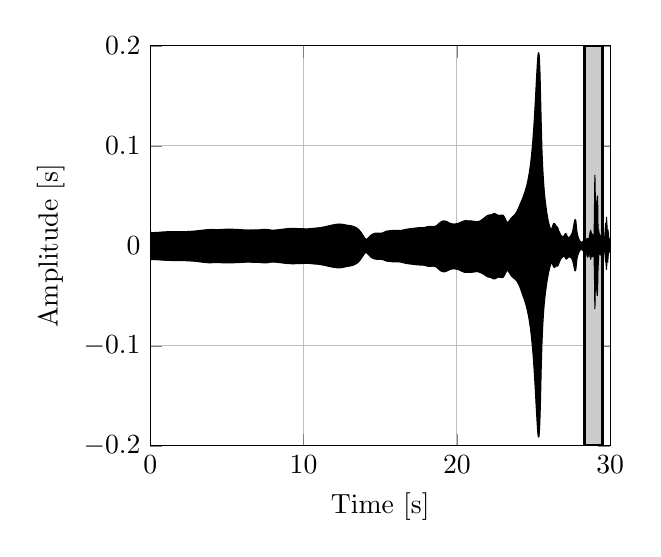
\begin{tikzpicture}

\begin{axis}[%
width=2.3in,
height=2in,
at={(1.011in,0.642in)},
scale only axis,
xmin=0,
xmax=30,
xmajorgrids,
ymin=-0.2,
ymax=0.2,
ymajorgrids,
xlabel={Time [s]},
ylabel={Amplitude [s]},
axis background/.style={fill=white}
]
\node[rectangle,draw, fill=black!20, minimum height=2in, minimum width=1pt, line width=1pt] at (axis cs:28.9,0) {};
\addplot[fill=black,draw=black,forget plot] plot table[row sep=crcr]{%
2.08333333333333e-05	0.0174441337585449\\
0.0250416666666667	0.013525128364563\\
0.0500625	0.013148307800293\\
0.0750833333333333	0.0131036043167114\\
0.100104166666667	0.0130690336227417\\
0.125125	0.0130878686904907\\
0.150145833333333	0.0131148099899292\\
0.175166666666667	0.0131456851959229\\
0.2001875	0.0131820440292358\\
0.225208333333333	0.0131937265396118\\
0.250229166666667	0.013242244720459\\
0.27525	0.0132321119308472\\
0.300270833333333	0.0132625102996826\\
0.325291666666667	0.0132992267608643\\
0.3503125	0.0133000612258911\\
0.375333333333333	0.0133060216903687\\
0.400354166666667	0.0133442878723145\\
0.425375	0.0133682489395142\\
0.450395833333333	0.0134040117263794\\
0.475416666666667	0.0134208202362061\\
0.5004375	0.0134366750717163\\
0.525458333333333	0.0134779214859009\\
0.550479166666667	0.013481616973877\\
0.5755	0.0135024785995483\\
0.600520833333333	0.0135313272476196\\
0.625541666666667	0.0135687589645386\\
0.6505625	0.0135985612869263\\
0.675583333333333	0.013633131980896\\
0.700604166666667	0.0136561393737793\\
0.725625	0.0136919021606445\\
0.750645833333333	0.0137306451797485\\
0.775666666666667	0.0137556791305542\\
0.8006875	0.01378333568573\\
0.825708333333333	0.0138041973114014\\
0.850729166666667	0.0138405561447144\\
0.87575	0.0138554573059082\\
0.900770833333333	0.0138554573059082\\
0.925791666666667	0.0138950347900391\\
0.9508125	0.0139113664627075\\
0.975833333333333	0.0139317512512207\\
1.00085416666667	0.0139557123184204\\
1.025875	0.0139747858047485\\
1.05089583333333	0.0140010118484497\\
1.07591666666667	0.0140320062637329\\
1.1009375	0.0140565633773804\\
1.12595833333333	0.0140770673751831\\
1.15097916666667	0.0140986442565918\\
1.176	0.0141662359237671\\
1.20102083333333	0.0141526460647583\\
1.22604166666667	0.0141149759292603\\
1.2510625	0.0141333341598511\\
1.27608333333333	0.0141546726226807\\
1.30110416666667	0.0141855478286743\\
1.326125	0.014235258102417\\
1.35114583333333	0.0142221450805664\\
1.37616666666667	0.0142310857772827\\
1.4011875	0.0142514705657959\\
1.42620833333333	0.0142489671707153\\
1.45122916666667	0.0142501592636108\\
1.47625	0.0142405033111572\\
1.50127083333333	0.0142426490783691\\
1.52629166666667	0.014230489730835\\
1.5513125	0.0142196416854858\\
1.57633333333333	0.0141897201538086\\
1.60135416666667	0.0141717195510864\\
1.626375	0.0141717195510864\\
1.65139583333333	0.0141562223434448\\
1.67641666666667	0.0141308307647705\\
1.7014375	0.0141433477401733\\
1.72645833333333	0.0141233205795288\\
1.75147916666667	0.0141158103942871\\
1.7765	0.0141146183013916\\
1.80152083333333	0.0140886306762695\\
1.82654166666667	0.0140882730484009\\
1.8515625	0.0140790939331055\\
1.87658333333333	0.0140920877456665\\
1.90160416666667	0.0140787363052368\\
1.926625	0.0140824317932129\\
1.95164583333333	0.014080286026001\\
1.97666666666667	0.0140800476074219\\
2.0016875	0.0140819549560547\\
2.02670833333333	0.0140724182128906\\
2.05172916666667	0.0140804052352905\\
2.07675	0.0140852928161621\\
2.10177083333333	0.0140907764434814\\
2.12679166666667	0.0141453742980957\\
2.1518125	0.0141433477401733\\
2.17683333333333	0.0141167640686035\\
2.20185416666667	0.014110803604126\\
2.226875	0.014117956161499\\
2.25189583333333	0.0141313076019287\\
2.27691666666667	0.01416015625\\
2.3019375	0.0141942501068115\\
2.32695833333333	0.0142010450363159\\
2.35197916666667	0.0142147541046143\\
2.377	0.0142277479171753\\
2.40202083333333	0.014255166053772\\
2.42704166666667	0.0142706632614136\\
2.4520625	0.0142948627471924\\
2.47708333333333	0.0143097639083862\\
2.50210416666667	0.014333963394165\\
2.527125	0.0143415927886963\\
2.55214583333333	0.0143803358078003\\
2.57716666666667	0.0144015550613403\\
2.6021875	0.0144282579421997\\
2.62720833333333	0.0144572257995605\\
2.65222916666667	0.0144776105880737\\
2.67725	0.0145164728164673\\
2.70227083333333	0.0145268440246582\\
2.72729166666667	0.0144838094711304\\
2.7523125	0.0145807266235352\\
2.77733333333333	0.0146057605743408\\
2.80235416666667	0.014631986618042\\
2.827375	0.0146661996841431\\
2.85239583333333	0.0147078037261963\\
2.87741666666667	0.0147354602813721\\
2.9024375	0.0147578716278076\\
2.92745833333333	0.0148038864135742\\
2.95247916666667	0.0148260593414307\\
2.9775	0.0148706436157227\\
3.00252083333333	0.0148930549621582\\
3.02754166666667	0.0149344205856323\\
3.0525625	0.0149737596511841\\
3.07758333333333	0.0150246620178223\\
3.10260416666667	0.0150657892227173\\
3.127625	0.0151075124740601\\
3.15264583333333	0.0151689052581787\\
3.17766666666667	0.0152368545532227\\
3.2026875	0.0152426958084106\\
3.22770833333333	0.0153077840805054\\
3.25272916666667	0.0153446197509766\\
3.27775	0.0153803825378418\\
3.30277083333333	0.0154129266738892\\
3.32779166666667	0.0154589414596558\\
3.3528125	0.0155411958694458\\
3.37783333333333	0.0155452489852905\\
3.40285416666667	0.0155919790267944\\
3.427875	0.0156158208847046\\
3.45289583333333	0.0156674385070801\\
3.47791666666667	0.0156955718994141\\
3.5029375	0.0157450437545776\\
3.52795833333333	0.0157967805862427\\
3.55297916666667	0.0158439874649048\\
3.578	0.0158843994140625\\
3.60302083333333	0.0159142017364502\\
3.62804166666667	0.0159745216369629\\
3.6530625	0.0160062313079834\\
3.67808333333333	0.0160480737686157\\
3.70310416666667	0.0160622596740723\\
3.728125	0.0160926580429077\\
3.75314583333333	0.0161361694335938\\
3.77816666666667	0.0161548852920532\\
3.8031875	0.0161689519882202\\
3.82820833333333	0.0162111520767212\\
3.85322916666667	0.0162196159362793\\
3.87825	0.0162382125854492\\
3.90327083333333	0.0162340402603149\\
3.92829166666667	0.0162550210952759\\
3.9533125	0.0162825584411621\\
3.97833333333333	0.016268253326416\\
4.00335416666667	0.0162605047225952\\
4.028375	0.0162662267684937\\
4.05339583333333	0.0162646770477295\\
4.07841666666667	0.0162562131881714\\
4.1034375	0.0162479877471924\\
4.12845833333333	0.0162286758422852\\
4.15347916666667	0.0162270069122314\\
4.1785	0.0162371397018433\\
4.20352083333333	0.0162290334701538\\
4.22854166666667	0.0162320137023926\\
4.2535625	0.0162011384963989\\
4.27858333333333	0.0161998271942139\\
4.30360416666667	0.0161756277084351\\
4.328625	0.0161881446838379\\
4.35364583333333	0.0161887407302856\\
4.37866666666667	0.0161789655685425\\
4.4036875	0.0161731243133545\\
4.42870833333333	0.0161886215209961\\
4.45372916666667	0.0162254571914673\\
4.47875	0.0162070989608765\\
4.50377083333333	0.0162215232849121\\
4.52879166666667	0.0162445306777954\\
4.5538125	0.0162478685379028\\
4.57883333333333	0.0162779092788696\\
4.60385416666667	0.0163146257400513\\
4.628875	0.0163321495056152\\
4.65389583333333	0.0163751840591431\\
4.67891666666667	0.0163940191268921\\
4.7039375	0.0164142847061157\\
4.72895833333333	0.0164343118667603\\
4.75397916666667	0.0164676904678345\\
4.779	0.0164873600006104\\
4.80402083333333	0.0164920091629028\\
4.82904166666667	0.0165045261383057\\
4.8540625	0.0165075063705444\\
4.87908333333333	0.0164927244186401\\
4.90410416666667	0.0165128707885742\\
4.929125	0.0165145397186279\\
4.95414583333333	0.0165392160415649\\
4.97916666666667	0.0165292024612427\\
5.0041875	0.0165307521820068\\
5.02920833333333	0.0165344476699829\\
5.05422916666667	0.0165383815765381\\
5.07925	0.0165324211120605\\
5.10427083333333	0.0165327787399292\\
5.12929166666667	0.0165436267852783\\
5.1543125	0.0165482759475708\\
5.17933333333333	0.0165408849716187\\
5.20435416666667	0.0165520906448364\\
5.229375	0.0165524482727051\\
5.25439583333333	0.0165770053863525\\
5.27941666666667	0.0165494680404663\\
5.3044375	0.0165427923202515\\
5.32945833333333	0.0165486335754395\\
5.35447916666667	0.016539454460144\\
5.3795	0.0165292024612427\\
5.40452083333333	0.0165024995803833\\
5.42954166666667	0.0165091753005981\\
5.4545625	0.0165070295333862\\
5.47958333333333	0.0164998769760132\\
5.50460416666667	0.0164941549301147\\
5.529625	0.0164831876754761\\
5.55464583333333	0.0164557695388794\\
5.57966666666667	0.0164422988891602\\
5.6046875	0.0164165496826172\\
5.62970833333333	0.0164107084274292\\
5.65472916666667	0.0163847208023071\\
5.67975	0.0163700580596924\\
5.70477083333333	0.0163614749908447\\
5.72979166666667	0.0163367986679077\\
5.7548125	0.0162984132766724\\
5.77983333333333	0.0162603855133057\\
5.80485416666667	0.0162379741668701\\
5.829875	0.0161999464035034\\
5.85489583333333	0.0161981582641602\\
5.87991666666667	0.0161627531051636\\
5.9049375	0.0161465406417847\\
5.92995833333333	0.016115665435791\\
5.95497916666667	0.0160897970199585\\
5.98	0.0160585641860962\\
6.00502083333333	0.0160255432128906\\
6.03004166666667	0.0159686803817749\\
6.0550625	0.0159963369369507\\
6.08008333333333	0.0159759521484375\\
6.10510416666667	0.0159282684326172\\
6.130125	0.015892505645752\\
6.15514583333333	0.0158891677856445\\
6.18016666666667	0.0158644914627075\\
6.2051875	0.0158466100692749\\
6.23020833333333	0.0158360004425049\\
6.25522916666667	0.0158376693725586\\
6.28025	0.0158051252365112\\
6.30527083333333	0.0157734155654907\\
6.33029166666667	0.0157642364501953\\
6.3553125	0.015750527381897\\
6.38033333333333	0.0157539844512939\\
6.40535416666667	0.0157500505447388\\
6.430375	0.0157680511474609\\
6.45539583333333	0.0157589912414551\\
6.48041666666667	0.0157626867294312\\
6.5054375	0.0157822370529175\\
6.53045833333333	0.0157740116119385\\
6.55547916666667	0.0157889127731323\\
6.5805	0.01578688621521\\
6.60552083333333	0.0157822370529175\\
6.63054166666667	0.015788197517395\\
6.6555625	0.0157915353775024\\
6.68058333333333	0.0158027410507202\\
6.70560416666667	0.0158090591430664\\
6.730625	0.0157994031906128\\
6.75564583333333	0.0158072710037231\\
6.78066666666667	0.0158181190490723\\
6.8056875	0.0157982110977173\\
6.83070833333333	0.0158140659332275\\
6.85572916666667	0.0158218145370483\\
6.88075	0.0158369541168213\\
6.90577083333333	0.015845775604248\\
6.93079166666667	0.0158636569976807\\
6.9558125	0.0158761739730835\\
6.98083333333333	0.0158882141113281\\
7.00585416666667	0.0158886909484863\\
7.030875	0.015921950340271\\
7.05589583333333	0.015964150428772\\
7.08091666666667	0.0159696340560913\\
7.1059375	0.0159767866134644\\
7.13095833333333	0.0160138607025146\\
7.15597916666667	0.0160485506057739\\
7.181	0.0161073207855225\\
7.20602083333333	0.0161236524581909\\
7.23104166666667	0.0161528587341309\\
7.2560625	0.0162006616592407\\
7.28108333333333	0.0162516832351685\\
7.30610416666667	0.0162925720214844\\
7.331125	0.0163209438323975\\
7.35614583333333	0.0163383483886719\\
7.38116666666667	0.0163733959197998\\
7.4061875	0.0163830518722534\\
7.43120833333333	0.0164109468460083\\
7.45622916666667	0.0164159536361694\\
7.48125	0.0164202451705933\\
7.50627083333333	0.01641845703125\\
7.53129166666667	0.0163898468017578\\
7.5563125	0.0163893699645996\\
7.58133333333333	0.0163614749908447\\
7.60635416666667	0.0163397789001465\\
7.631375	0.016291618347168\\
7.65639583333333	0.0162471532821655\\
7.68141666666667	0.0162198543548584\\
7.7064375	0.016148567199707\\
7.73145833333333	0.0160896778106689\\
7.75647916666667	0.016048789024353\\
7.7815	0.0159863233566284\\
7.80652083333333	0.0158941745758057\\
7.83154166666667	0.0158556699752808\\
7.8565625	0.0158106088638306\\
7.88158333333333	0.0157514810562134\\
7.90660416666667	0.0157146453857422\\
7.931625	0.0156705379486084\\
7.95664583333333	0.015657901763916\\
7.98166666666667	0.0156430006027222\\
8.0066875	0.015637993812561\\
8.03170833333333	0.0156441926956177\\
8.05672916666667	0.015630841255188\\
8.08175	0.0156583786010742\\
8.10677083333333	0.0156680345535278\\
8.13179166666667	0.0156958103179932\\
8.1568125	0.0157588720321655\\
8.18183333333333	0.0157665014266968\\
8.20685416666667	0.015811562538147\\
8.231875	0.0158299207687378\\
8.25689583333333	0.0158756971359253\\
8.28191666666667	0.0159240961074829\\
8.3069375	0.0159738063812256\\
8.33195833333333	0.0160108804702759\\
8.35697916666667	0.01605224609375\\
8.382	0.0161123275756836\\
8.40702083333333	0.0161582231521606\\
8.43204166666667	0.0161970853805542\\
8.4570625	0.0162638425827026\\
8.48208333333333	0.0163058042526245\\
8.50710416666667	0.0163264274597168\\
8.532125	0.0163748264312744\\
8.55714583333333	0.016425609588623\\
8.58216666666667	0.0164724588394165\\
8.6071875	0.0164806842803955\\
8.63220833333333	0.0165771245956421\\
8.65722916666667	0.0166155099868774\\
8.68225	0.0166538953781128\\
8.70727083333333	0.0166980028152466\\
8.73229166666667	0.0167548656463623\\
8.7573125	0.0168157815933228\\
8.78233333333333	0.0168620347976685\\
8.80735416666667	0.0168946981430054\\
8.832375	0.0169271230697632\\
8.85739583333333	0.0169821977615356\\
8.88241666666667	0.0170294046401978\\
8.9074375	0.0170701742172241\\
8.93245833333333	0.0171375274658203\\
8.95747916666667	0.0171374082565308\\
8.9825	0.0171587467193604\\
9.00752083333333	0.0172109603881836\\
9.03254166666667	0.017237663269043\\
9.0575625	0.0172935724258423\\
9.08258333333333	0.0173063278198242\\
9.10760416666667	0.0173218250274658\\
9.132625	0.0173497200012207\\
9.15764583333333	0.0173478126525879\\
9.18266666666667	0.0173822641372681\\
9.2076875	0.0173777341842651\\
9.23270833333333	0.0174020528793335\\
9.25772916666667	0.0174028873443604\\
9.28275	0.0174024105072021\\
9.30777083333333	0.0174020528793335\\
9.33279166666667	0.017372727394104\\
9.3578125	0.017397403717041\\
9.38283333333333	0.017382025718689\\
9.40785416666667	0.0173285007476807\\
9.432875	0.017330527305603\\
9.45789583333333	0.0173323154449463\\
9.48291666666667	0.0173298120498657\\
9.5079375	0.0173071622848511\\
9.53295833333333	0.0172946453094482\\
9.55797916666667	0.0172981023788452\\
9.583	0.0172525644302368\\
9.60802083333333	0.0172533988952637\\
9.63304166666667	0.0172268152236938\\
9.6580625	0.0172150135040283\\
9.68308333333333	0.0172126293182373\\
9.70810416666667	0.0172011852264404\\
9.733125	0.0171859264373779\\
9.75814583333333	0.0171804428100586\\
9.78316666666667	0.0171525478363037\\
9.8081875	0.0171377658843994\\
9.83320833333334	0.0171386003494263\\
9.85822916666667	0.0171124935150146\\
9.88325	0.0171166658401489\\
9.90827083333333	0.0170993804931641\\
9.93329166666667	0.0170944929122925\\
9.9583125	0.0170706510543823\\
9.98333333333333	0.0170501470565796\\
10.0083541666667	0.0170356035232544\\
10.033375	0.0169914960861206\\
10.0583958333333	0.0170005559921265\\
10.0834166666667	0.0170102119445801\\
10.1084375	0.0169705152511597\\
10.1334583333333	0.0169491767883301\\
10.1584791666667	0.0169483423233032\\
10.1835	0.0169246196746826\\
10.2085208333333	0.0169349908828735\\
10.2335416666667	0.016913890838623\\
10.2585625	0.016938328742981\\
10.2835833333333	0.0169572830200195\\
10.3086041666667	0.0169775485992432\\
10.333625	0.016999363899231\\
10.3586458333333	0.0170327425003052\\
10.3836666666667	0.0170744657516479\\
10.4086875	0.0170915126800537\\
10.4337083333333	0.0171260833740234\\
10.4587291666667	0.0171712636947632\\
10.48375	0.0172317028045654\\
10.5087708333333	0.0172442197799683\\
10.5337916666667	0.0172771215438843\\
10.5588125	0.017345666885376\\
10.5838333333333	0.0173889398574829\\
10.6088541666667	0.0174278020858765\\
10.633875	0.0174736976623535\\
10.6588958333333	0.0175179243087769\\
10.6839166666667	0.017504096031189\\
10.7089375	0.0175975561141968\\
10.7339583333333	0.0176342725753784\\
10.7589791666667	0.0176651477813721\\
10.784	0.0177170038223267\\
10.8090208333333	0.0177382230758667\\
10.8340416666667	0.0177578926086426\\
10.8590625	0.0177834033966064\\
10.8840833333333	0.0178287029266357\\
10.9091041666667	0.0178596973419189\\
10.934125	0.0178934335708618\\
10.9591458333333	0.0179351568222046\\
10.9841666666667	0.0179930925369263\\
11.0091875	0.0180190801620483\\
11.0342083333333	0.0180590152740479\\
11.0592291666667	0.0180873870849609\\
11.08425	0.0181617736816406\\
11.1092708333333	0.0181983709335327\\
11.1342916666667	0.0182547569274902\\
11.1593125	0.018323540687561\\
11.1843333333333	0.018383264541626\\
11.2093541666667	0.0184645652770996\\
11.234375	0.0185511112213135\\
11.2593958333333	0.0186281204223633\\
11.2844166666667	0.0186648368835449\\
11.3094375	0.0187809467315674\\
11.3344583333333	0.0188539028167725\\
11.3594791666667	0.0189625024795532\\
11.3845	0.0190408229827881\\
11.4095208333333	0.0191167593002319\\
11.4345416666667	0.0191928148269653\\
11.4595625	0.019289493560791\\
11.4845833333333	0.0194246768951416\\
11.5096041666667	0.0194790363311768\\
11.534625	0.0195668935775757\\
11.5596458333333	0.0196346044540405\\
11.5846666666667	0.0197362899780273\\
11.6096875	0.0198198556900024\\
11.6347083333333	0.0198944807052612\\
11.6597291666667	0.0199992656707764\\
11.68475	0.0200852155685425\\
11.7097708333333	0.0201708078384399\\
11.7347916666667	0.0202442407608032\\
11.7598125	0.0203417539596558\\
11.7848333333333	0.020447850227356\\
11.8098541666667	0.0205179452896118\\
11.834875	0.020601749420166\\
11.8598958333333	0.0206559896469116\\
11.8849166666667	0.0207802057266235\\
11.9099375	0.0208553075790405\\
11.9349583333333	0.0209276676177979\\
11.9599791666667	0.0209884643554688\\
11.985	0.0210902690887451\\
12.0100208333333	0.0211566686630249\\
12.0350416666667	0.0212430953979492\\
12.0600625	0.0213093757629395\\
12.0850833333333	0.0213801860809326\\
12.1101041666667	0.0214052200317383\\
12.135125	0.0214844942092896\\
12.1601458333333	0.0215476751327515\\
12.1851666666667	0.0216346979141235\\
12.2101875	0.0216710567474365\\
12.2352083333333	0.0217214822769165\\
12.2602291666667	0.0217512845993042\\
12.28525	0.0217370986938477\\
12.3102708333333	0.0217386484146118\\
12.3352916666667	0.0217440128326416\\
12.3603125	0.0217629671096802\\
12.3853333333333	0.0217190980911255\\
12.4103541666667	0.0217164754867554\\
12.435375	0.0216363668441772\\
12.4603958333333	0.0216211080551147\\
12.4854166666667	0.021581768989563\\
12.5104375	0.0215216875076294\\
12.5354583333333	0.021467924118042\\
12.5604791666667	0.0213643312454224\\
12.5855	0.021304726600647\\
12.6105208333333	0.0212384462356567\\
12.6355416666667	0.0211762189865112\\
12.6605625	0.0210961103439331\\
12.6855833333333	0.0210355520248413\\
12.7106041666667	0.0209527015686035\\
12.735625	0.0208666324615479\\
12.7606458333333	0.0208185911178589\\
12.7856666666667	0.0207582712173462\\
12.8106875	0.0206890106201172\\
12.8357083333333	0.0206308364868164\\
12.8607291666667	0.0205554962158203\\
12.88575	0.0205261707305908\\
12.9107708333333	0.0204222202301025\\
12.9357916666667	0.0204188823699951\\
12.9608125	0.0203204154968262\\
12.9858333333333	0.0202691555023193\\
13.0108541666667	0.0202019214630127\\
13.035875	0.0201456546783447\\
13.0608958333333	0.0200655460357666\\
13.0859166666667	0.0200191736221313\\
13.1109375	0.0199253559112549\\
13.1359583333333	0.0198445320129395\\
13.1609791666667	0.0197505950927734\\
13.186	0.0197038650512695\\
13.2110208333333	0.0195786952972412\\
13.2360416666667	0.019476056098938\\
13.2610625	0.0193073749542236\\
13.2860833333333	0.0191764831542969\\
13.3111041666667	0.0190207958221436\\
13.336125	0.0188961029052734\\
13.3611458333333	0.0186749696731567\\
13.3861666666667	0.0185122489929199\\
13.4111875	0.0183169841766357\\
13.4362083333333	0.0180661678314209\\
13.4612291666667	0.017853856086731\\
13.48625	0.0175918340682983\\
13.5112708333333	0.0173110961914062\\
13.5362916666667	0.0169925689697266\\
13.5613125	0.0166597366333008\\
13.5863333333333	0.0163099765777588\\
13.6113541666667	0.0159174203872681\\
13.636375	0.0155293941497803\\
13.6613958333333	0.0150763988494873\\
13.6864166666667	0.0146143436431885\\
13.7114375	0.014168381690979\\
13.7364583333333	0.0136096477508545\\
13.7614791666667	0.0130655765533447\\
13.7865	0.0125436782836914\\
13.8115208333333	0.0119357109069824\\
13.8365416666667	0.0113338232040405\\
13.8615625	0.0106756687164307\\
13.8865833333333	0.0100915431976318\\
13.9116041666667	0.00947129726409912\\
13.936625	0.00886750221252441\\
13.9616458333333	0.00825822353363037\\
13.9866666666667	0.00778257846832275\\
14.0116875	0.00735759735107422\\
14.0367083333333	0.00696361064910889\\
14.0617291666667	0.00667524337768555\\
14.08675	0.00652050971984863\\
14.1117708333333	0.00652647018432617\\
14.1367916666667	0.00670945644378662\\
14.1618125	0.00699913501739502\\
14.1868333333333	0.00733792781829834\\
14.2118541666667	0.0077139139175415\\
14.236875	0.00815272331237793\\
14.2618958333333	0.00860869884490967\\
14.2869166666667	0.00900518894195557\\
14.3119375	0.00939702987670898\\
14.3369583333333	0.00978922843933105\\
14.3619791666667	0.0101321935653687\\
14.387	0.0104804039001465\\
14.4120208333333	0.0107772350311279\\
14.4370416666667	0.0110471248626709\\
14.4620625	0.0112928152084351\\
14.4870833333333	0.0115351676940918\\
14.5121041666667	0.0117450952529907\\
14.537125	0.0118981599807739\\
14.5621458333333	0.0120600461959839\\
14.5871666666667	0.0121918916702271\\
14.6121875	0.0123043060302734\\
14.6372083333333	0.0123888254165649\\
14.6622291666667	0.0124760866165161\\
14.68725	0.0125365257263184\\
14.7122708333333	0.0126163959503174\\
14.7372916666667	0.0126279592514038\\
14.7623125	0.0126475095748901\\
14.7873333333333	0.0126579999923706\\
14.8123541666667	0.0126771926879883\\
14.837375	0.0126643180847168\\
14.8623958333333	0.0126522779464722\\
14.8874166666667	0.0126442909240723\\
14.9124375	0.0126438140869141\\
14.9374583333333	0.0126296281814575\\
14.9624791666667	0.0126005411148071\\
14.9875	0.0125808715820312\\
15.0125208333333	0.0125870704650879\\
15.0375416666667	0.0125871896743774\\
15.0625625	0.0126022100448608\\
15.0875833333333	0.0126547813415527\\
15.1126041666667	0.0127360820770264\\
15.137625	0.0128141641616821\\
15.1626458333333	0.0129730701446533\\
15.1876666666667	0.0131022930145264\\
15.2126875	0.0132739543914795\\
15.2377083333333	0.0134528875350952\\
15.2627291666667	0.0136306285858154\\
15.28775	0.0138425827026367\\
15.3127708333333	0.0140299797058105\\
15.3377916666667	0.014187216758728\\
15.3628125	0.0143324136734009\\
15.3878333333333	0.0144814252853394\\
15.4128541666667	0.0145851373672485\\
15.437875	0.0147069692611694\\
15.4628958333333	0.0147304534912109\\
15.4879166666667	0.014826774597168\\
15.5129375	0.0148801803588867\\
15.5379583333333	0.0149414539337158\\
15.5629791666667	0.0149836540222168\\
15.588	0.0150250196456909\\
15.6130208333333	0.0150867700576782\\
15.6380416666667	0.0151267051696777\\
15.6630625	0.0151498317718506\\
15.6880833333333	0.0151907205581665\\
15.7131041666667	0.0152368545532227\\
15.738125	0.0152875185012817\\
15.7631458333333	0.0153127908706665\\
15.7881666666667	0.015317440032959\\
15.8131875	0.0153570175170898\\
15.8382083333333	0.0153809785842896\\
15.8632291666667	0.0153845548629761\\
15.88825	0.0154021978378296\\
15.9132708333333	0.0154201984405518\\
15.9382916666667	0.0154287815093994\\
15.9633125	0.0154200792312622\\
15.9883333333333	0.0154142379760742\\
16.0133541666667	0.0154227018356323\\
16.038375	0.0153951644897461\\
16.0633958333333	0.0153549909591675\\
16.0884166666667	0.0153504610061646\\
16.1134375	0.015299916267395\\
16.1384583333333	0.0152820348739624\\
16.1634791666667	0.0152640342712402\\
16.1885	0.0152740478515625\\
16.2135208333333	0.0152524709701538\\
16.2385416666667	0.0152736902236938\\
16.2635625	0.0152624845504761\\
16.2885833333333	0.0152912139892578\\
16.3136041666667	0.0153496265411377\\
16.338625	0.015373706817627\\
16.3636458333333	0.0154263973236084\\
16.3886666666667	0.0154972076416016\\
16.4136875	0.0155841112136841\\
16.4387083333333	0.0156378746032715\\
16.4637291666667	0.01569664478302\\
16.48875	0.015790581703186\\
16.5137708333333	0.0158723592758179\\
16.5387916666667	0.0159751176834106\\
16.5638125	0.0160551071166992\\
16.5888333333333	0.0161577463150024\\
16.6138541666667	0.0162507295608521\\
16.638875	0.0163224935531616\\
16.6638958333333	0.0163685083389282\\
16.6889166666667	0.0164364576339722\\
16.7139375	0.0165036916732788\\
16.7389583333333	0.0165603160858154\\
16.7639791666667	0.0166410207748413\\
16.789	0.0167248249053955\\
16.8140208333333	0.0167744159698486\\
16.8390416666667	0.016828179359436\\
16.8640625	0.0168788433074951\\
16.8890833333333	0.0169576406478882\\
16.9141041666667	0.016994833946228\\
16.939125	0.0170410871505737\\
16.9641458333333	0.0170806646347046\\
16.9891666666667	0.017139196395874\\
17.0141875	0.0172109603881836\\
17.0392083333333	0.0172618627548218\\
17.0642291666667	0.0173348188400269\\
17.08925	0.0173755884170532\\
17.1142708333333	0.0174448490142822\\
17.1392916666667	0.0174486637115479\\
17.1643125	0.0174803733825684\\
17.1893333333333	0.017526388168335\\
17.2143541666667	0.0175930261611938\\
17.239375	0.0176322460174561\\
17.2643958333333	0.0176610946655273\\
17.2894166666667	0.0177028179168701\\
17.3144375	0.0177712440490723\\
17.3394583333333	0.017817497253418\\
17.3644791666667	0.0178496837615967\\
17.3895	0.0178635120391846\\
17.4145208333333	0.0179288387298584\\
17.4395416666667	0.017961859703064\\
17.4645625	0.017999529838562\\
17.4895833333333	0.018022894859314\\
17.5146041666667	0.018062949180603\\
17.539625	0.0180728435516357\\
17.5646458333333	0.01810622215271\\
17.5896666666667	0.0180763006210327\\
17.6146875	0.0180631875991821\\
17.6397083333333	0.0180815458297729\\
17.6647291666667	0.0180732011795044\\
17.68975	0.0180611610412598\\
17.7147708333333	0.0180732011795044\\
17.7397916666667	0.0180991888046265\\
17.7648125	0.018126368522644\\
17.7898333333333	0.0181397199630737\\
17.8148541666667	0.0181893110275269\\
17.839875	0.0182832479476929\\
17.8648958333333	0.0183231830596924\\
17.8899166666667	0.0183992385864258\\
17.9149375	0.0184700489044189\\
17.9399583333333	0.0185521841049194\\
17.9649791666667	0.0186257362365723\\
17.99	0.0187492370605469\\
18.0150208333333	0.0188664197921753\\
18.0400416666667	0.0189815759658813\\
18.0650625	0.0190328359603882\\
18.0900833333333	0.0191329717636108\\
18.1151041666667	0.0192264318466187\\
18.140125	0.0192656517028809\\
18.1651458333333	0.0192974805831909\\
18.1901666666667	0.0193121433258057\\
18.2151875	0.0193363428115845\\
18.2402083333333	0.0193533897399902\\
18.2652291666667	0.0193248987197876\\
18.29025	0.0193346738815308\\
18.3152708333333	0.0193099975585938\\
18.3402916666667	0.0192739963531494\\
18.3653125	0.0192720890045166\\
18.3903333333333	0.0192562341690063\\
18.4153541666667	0.0192611217498779\\
18.440375	0.0192636251449585\\
18.4653958333333	0.0192465782165527\\
18.4904166666667	0.0192739963531494\\
18.5154375	0.0192666053771973\\
18.5404583333333	0.0192996263504028\\
18.5654791666667	0.0193842649459839\\
18.5905	0.0194982290267944\\
18.6155208333333	0.0196996927261353\\
18.6405416666667	0.0198712348937988\\
18.6655625	0.0201015472412109\\
18.6905833333333	0.02039635181427\\
18.7156041666667	0.0207115411758423\\
18.740625	0.02104651927948\\
18.7656458333333	0.0213632583618164\\
18.7906666666667	0.0217374563217163\\
18.8156875	0.0221004486083984\\
18.8407083333333	0.0224542617797852\\
18.8657291666667	0.0227910280227661\\
18.89075	0.023115873336792\\
18.9157708333333	0.0234055519104004\\
18.9407916666667	0.0236350297927856\\
18.9658125	0.0238840579986572\\
18.9908333333333	0.0240856409072876\\
19.0158541666667	0.0243097543716431\\
19.040875	0.0244883298873901\\
19.0658958333333	0.0246367454528809\\
19.0909166666667	0.0247553586959839\\
19.1159375	0.0248157978057861\\
19.1409583333333	0.0248211622238159\\
19.1659791666667	0.0248291492462158\\
19.191	0.0247656106948853\\
19.2160208333333	0.0247126817703247\\
19.2410416666667	0.0246188640594482\\
19.2660625	0.0245308876037598\\
19.2910833333333	0.024416446685791\\
19.3161041666667	0.0243091583251953\\
19.341125	0.0241603851318359\\
19.3661458333333	0.0239905118942261\\
19.3911666666667	0.0237839221954346\\
19.4161875	0.0236095190048218\\
19.4412083333333	0.0234092473983765\\
19.4662291666667	0.0231764316558838\\
19.49125	0.0229754447937012\\
19.5162708333333	0.022815465927124\\
19.5412916666667	0.0226483345031738\\
19.5663125	0.0224692821502686\\
19.5913333333333	0.0223290920257568\\
19.6163541666667	0.0222113132476807\\
19.641375	0.0221070051193237\\
19.6663958333333	0.0220341682434082\\
19.6914166666667	0.0219175815582275\\
19.7164375	0.0218663215637207\\
19.7414583333333	0.0218421220779419\\
19.7664791666667	0.0217581987380981\\
19.7915	0.021744966506958\\
19.8165208333333	0.0217596292495728\\
19.8415416666667	0.0217770338058472\\
19.8665625	0.0217828750610352\\
19.8915833333333	0.0218362808227539\\
19.9166041666667	0.0218791961669922\\
19.941625	0.0219467878341675\\
19.9666458333333	0.0220240354537964\\
19.9916666666667	0.0220874547958374\\
20.0166875	0.0221959352493286\\
20.0417083333333	0.022313117980957\\
20.0667291666667	0.0224117040634155\\
20.09175	0.0225427150726318\\
20.1167708333333	0.0226690769195557\\
20.1417916666667	0.0228263139724731\\
20.1668125	0.0229573249816895\\
20.1918333333333	0.0231013298034668\\
20.2168541666667	0.0232757329940796\\
20.241875	0.0234352350234985\\
20.2668958333333	0.0236291885375977\\
20.2919166666667	0.0237768888473511\\
20.3169375	0.023958683013916\\
20.3419583333333	0.0241364240646362\\
20.3669791666667	0.0242964029312134\\
20.392	0.0244518518447876\\
20.4170208333333	0.0246180295944214\\
20.4420416666667	0.0247514247894287\\
20.4670625	0.0248813629150391\\
20.4920833333333	0.0249801874160767\\
20.5171041666667	0.0250335931777954\\
20.542125	0.0250766277313232\\
20.5671458333333	0.0250948667526245\\
20.5921666666667	0.0251015424728394\\
20.6171875	0.0250868797302246\\
20.6422083333333	0.025084376335144\\
20.6672291666667	0.0250357389450073\\
20.69225	0.0249865055084229\\
20.7172708333333	0.0249638557434082\\
20.7422916666667	0.0249263048171997\\
20.7673125	0.0249083042144775\\
20.7923333333333	0.0248900651931763\\
20.8173541666667	0.0248545408248901\\
20.842375	0.0248538255691528\\
20.8673958333333	0.0248371362686157\\
20.8924166666667	0.0248321294784546\\
20.9174375	0.0248321294784546\\
20.9424583333333	0.0248123407363892\\
20.9674791666667	0.0248016119003296\\
20.9925	0.0247378349304199\\
21.0175208333333	0.0246872901916504\\
21.0425416666667	0.0246568918228149\\
21.0675625	0.0245620012283325\\
21.0925833333333	0.0245187282562256\\
21.1176041666667	0.0244406461715698\\
21.142625	0.0243560075759888\\
21.1676458333333	0.0242875814437866\\
21.1926666666667	0.0241986513137817\\
21.2176875	0.0241419076919556\\
21.2427083333333	0.0241051912307739\\
21.2677291666667	0.0240743160247803\\
21.29275	0.0240596532821655\\
21.3177708333333	0.0240672826766968\\
21.3427916666667	0.0241365432739258\\
21.3678125	0.0242211818695068\\
21.3928333333333	0.0242770910263062\\
21.4178541666667	0.0243664979934692\\
21.442875	0.0245187282562256\\
21.4678958333333	0.0246692895889282\\
21.4929166666667	0.0248323678970337\\
21.5179375	0.0250157117843628\\
21.5429583333333	0.0251970291137695\\
21.5679791666667	0.0254095792770386\\
21.593	0.0256576538085938\\
21.6180208333333	0.0259164571762085\\
21.6430416666667	0.0261667966842651\\
21.6680625	0.0264409780502319\\
21.6930833333333	0.0267170667648315\\
21.7181041666667	0.0269858837127686\\
21.743125	0.0273033380508423\\
21.7681458333333	0.0276157855987549\\
21.7931666666667	0.0278679132461548\\
21.8181875	0.0282278060913086\\
21.8432083333333	0.0285413265228271\\
21.8682291666667	0.0288461446762085\\
21.89325	0.029139518737793\\
21.9182708333333	0.0294617414474487\\
21.9432916666667	0.0297086238861084\\
21.9683125	0.0300043821334839\\
21.9933333333333	0.0302213430404663\\
22.0183541666667	0.0304399728775024\\
22.043375	0.0305919647216797\\
22.0683958333333	0.0306967496871948\\
22.0934166666667	0.0307843685150146\\
22.1184375	0.0307987928390503\\
22.1434583333333	0.030825138092041\\
22.1684791666667	0.0308159589767456\\
22.1935	0.0308229923248291\\
22.2185208333333	0.0309444665908813\\
22.2435416666667	0.0311071872711182\\
22.2685625	0.0312448740005493\\
22.2935833333333	0.0314546823501587\\
22.3186041666667	0.0316667556762695\\
22.343625	0.0318219661712646\\
22.3686458333333	0.0320000648498535\\
22.3936666666667	0.0320919752120972\\
22.4186875	0.0321664810180664\\
22.4437083333333	0.0321915149688721\\
22.4687291666667	0.0321606397628784\\
22.49375	0.0321078300476074\\
22.5187708333333	0.031922459602356\\
22.5437916666667	0.0317248106002808\\
22.5688125	0.031496524810791\\
22.5938333333333	0.0312548875808716\\
22.6188541666667	0.0311131477355957\\
22.643875	0.0308171510696411\\
22.6688958333333	0.030713677406311\\
22.6939166666667	0.030561089515686\\
22.7189375	0.0304679870605469\\
22.7439583333333	0.0304421186447144\\
22.7689791666667	0.0303603410720825\\
22.794	0.0303953886032104\\
22.8190208333333	0.0304563045501709\\
22.8440416666667	0.0305156707763672\\
22.8690625	0.0305367708206177\\
22.8940833333333	0.0306057929992676\\
22.9191041666667	0.0306382179260254\\
22.944125	0.0306912660598755\\
22.9691458333333	0.0306316614151001\\
22.9941666666667	0.0306066274642944\\
23.0191875	0.0304591655731201\\
23.0442083333333	0.0300365686416626\\
23.0692291666667	0.0294849872589111\\
23.09425	0.0287594795227051\\
23.1192708333333	0.0279767513275146\\
23.1442916666667	0.027154803276062\\
23.1693125	0.0264017581939697\\
23.1943333333333	0.0256999731063843\\
23.2193541666667	0.0246617794036865\\
23.244375	0.0238051414489746\\
23.2693958333333	0.0236220359802246\\
23.2944166666667	0.0233170986175537\\
23.3194375	0.0234898328781128\\
23.3444583333333	0.0237802267074585\\
23.3694791666667	0.0241098403930664\\
23.3945	0.024639368057251\\
23.4195208333333	0.0251232385635376\\
23.4445416666667	0.0256147384643555\\
23.4695625	0.0261942148208618\\
23.4945833333333	0.0267441272735596\\
23.5196041666667	0.0272728204727173\\
23.544625	0.0277079343795776\\
23.5696458333333	0.0281523466110229\\
23.5946666666667	0.0285365581512451\\
23.6196875	0.0288980007171631\\
23.6447083333333	0.0291863679885864\\
23.6697291666667	0.0294959545135498\\
23.69475	0.029880166053772\\
23.7197708333333	0.0302121639251709\\
23.7447916666667	0.0305644273757935\\
23.7698125	0.0310232639312744\\
23.7948333333333	0.0315340757369995\\
23.8198541666667	0.0320580005645752\\
23.844875	0.0326471328735352\\
23.8698958333333	0.0332018136978149\\
23.8949166666667	0.0337858200073242\\
23.9199375	0.0345264673233032\\
23.9449583333333	0.0352761745452881\\
23.9699791666667	0.0361440181732178\\
23.995	0.0370364189147949\\
24.0200208333333	0.0377423763275146\\
24.0450416666667	0.0387363433837891\\
24.0700625	0.0396305322647095\\
24.0950833333333	0.0405175685882568\\
24.1201041666667	0.041479229927063\\
24.145125	0.0423545837402344\\
24.1701458333333	0.0432147979736328\\
24.1951666666667	0.044137716293335\\
24.2201875	0.0450013875961304\\
24.2452083333333	0.0459293127059937\\
24.2702291666667	0.0469129085540771\\
24.29525	0.0479274988174438\\
24.3202708333333	0.0489280223846436\\
24.3452916666667	0.0500307083129883\\
24.3703125	0.0510417222976685\\
24.3953333333333	0.052181601524353\\
24.4203541666667	0.0532969236373901\\
24.445375	0.0544567108154297\\
24.4703958333333	0.0556988716125488\\
24.4954166666667	0.056898832321167\\
24.5204375	0.0582900047302246\\
24.5454583333333	0.0596746206283569\\
24.5704791666667	0.0611917972564697\\
24.5955	0.0627651214599609\\
24.6205208333333	0.0645843744277954\\
24.6455416666667	0.0664654970169067\\
24.6705625	0.0684857368469238\\
24.6955833333333	0.0705987215042114\\
24.7206041666667	0.0729748010635376\\
24.745625	0.0752949714660645\\
24.7706458333333	0.0780850648880005\\
24.7956666666667	0.0809968709945679\\
24.8206875	0.084004282951355\\
24.8457083333333	0.0875474214553833\\
24.8707291666667	0.0909876823425293\\
24.89575	0.0951199531555176\\
24.9207708333333	0.0991923809051514\\
24.9457916666667	0.103655219078064\\
24.9708125	0.108772873878479\\
24.9958333333333	0.114107251167297\\
25.0208541666667	0.119699358940125\\
25.045875	0.125730037689209\\
25.0708958333333	0.132137656211853\\
25.0959166666667	0.139050245285034\\
25.1209375	0.146229147911072\\
25.1459583333333	0.153596758842468\\
25.1709791666667	0.161020040512085\\
25.196	0.168261528015137\\
25.2210208333333	0.175299406051636\\
25.2460416666667	0.181927919387817\\
25.2710625	0.187173366546631\\
25.2960833333333	0.191585659980774\\
25.3211041666667	0.192880272865295\\
25.346125	0.192724227905273\\
25.3711458333333	0.189618349075317\\
25.3961666666667	0.181955933570862\\
25.4211875	0.171445846557617\\
25.4462083333333	0.155550122261047\\
25.4712291666667	0.139785528182983\\
25.49625	0.123754620552063\\
25.5212708333333	0.109553933143616\\
25.5462916666667	0.0963232517242432\\
25.5713125	0.086665153503418\\
25.5963333333333	0.0784014463424683\\
25.6213541666667	0.071405291557312\\
25.646375	0.0651895999908447\\
25.6713958333333	0.0598506927490234\\
25.6964166666667	0.0547468662261963\\
25.7214375	0.050620436668396\\
25.7464583333333	0.0471398830413818\\
25.7714791666667	0.043710470199585\\
25.7965	0.0407135486602783\\
25.8215208333333	0.0378057956695557\\
25.8465416666667	0.0348886251449585\\
25.8715625	0.0322417020797729\\
25.8965833333333	0.0300600528717041\\
25.9216041666667	0.0277225971221924\\
25.946625	0.025759220123291\\
25.9716458333333	0.0239880084991455\\
25.9966666666667	0.0221370458602905\\
26.0216875	0.0206685066223145\\
26.0467083333333	0.0193742513656616\\
26.0717291666667	0.0183048248291016\\
26.09675	0.0174481868743896\\
26.1217708333333	0.0168154239654541\\
26.1467916666667	0.0165709257125854\\
26.1718125	0.0168967247009277\\
26.1968333333333	0.0176175832748413\\
26.2218541666667	0.0186170339584351\\
26.246875	0.0197421312332153\\
26.2718958333333	0.0208824872970581\\
26.2969166666667	0.0218906402587891\\
26.3219375	0.0222227573394775\\
26.3469583333333	0.0223579406738281\\
26.3719791666667	0.0221942663192749\\
26.397	0.0217078924179077\\
26.4220208333333	0.0209922790527344\\
26.4470416666667	0.0202728509902954\\
26.4720625	0.0196545124053955\\
26.4970833333333	0.0193988084793091\\
26.5221041666667	0.0191034078598022\\
26.547125	0.0187299251556396\\
26.5721458333333	0.0180537700653076\\
26.5971666666667	0.0168862342834473\\
26.6221875	0.015802264213562\\
26.6472083333333	0.0147438049316406\\
26.6722291666667	0.0138993263244629\\
26.69725	0.0131711959838867\\
26.7222708333333	0.0123679637908936\\
26.7472916666667	0.0115710496902466\\
26.7723125	0.0107738971710205\\
26.7973333333333	0.0101497173309326\\
26.8223541666667	0.00979006290435791\\
26.847375	0.00962471961975098\\
26.8723958333333	0.00949633121490479\\
26.8974166666667	0.00931215286254883\\
26.9224375	0.00916421413421631\\
26.9474583333333	0.00920677185058594\\
26.9724791666667	0.00953972339630127\\
26.9975	0.0102084875106812\\
27.0225208333333	0.0108667612075806\\
27.0475416666667	0.0115419626235962\\
27.0725625	0.0120722055435181\\
27.0975833333333	0.0121549367904663\\
27.1226041666667	0.0118545293807983\\
27.147625	0.0111083984375\\
27.1726458333333	0.0101121664047241\\
27.1976666666667	0.0093076229095459\\
27.2226875	0.00873386859893799\\
27.2477083333333	0.00842678546905518\\
27.2727291666667	0.00834882259368896\\
27.29775	0.00836217403411865\\
27.3227708333333	0.00848746299743652\\
27.3477916666667	0.00875973701477051\\
27.3728125	0.0090184211730957\\
27.3978333333333	0.00947034358978271\\
27.4228541666667	0.00991213321685791\\
27.447875	0.0106494426727295\\
27.4728958333333	0.0113028287887573\\
27.4979166666667	0.012182354927063\\
27.5229375	0.0131195783615112\\
27.5479583333333	0.0144155025482178\\
27.5729791666667	0.0162382125854492\\
27.598	0.0181559324264526\\
27.6230208333333	0.0203871726989746\\
27.6480416666667	0.0227947235107422\\
27.6730625	0.0248361825942993\\
27.6980833333333	0.0259034633636475\\
27.7231041666667	0.0261249542236328\\
27.748125	0.0256080627441406\\
27.7731458333333	0.0226942300796509\\
27.7981666666667	0.0178313255310059\\
27.8231875	0.0147879123687744\\
27.8482083333333	0.0123029947280884\\
27.8732291666667	0.0105404853820801\\
27.89825	0.00934135913848877\\
27.9232708333333	0.00792503356933594\\
27.9482916666667	0.00695645809173584\\
27.9733125	0.00611364841461182\\
27.9983333333333	0.00526881217956543\\
28.0233541666667	0.00476109981536865\\
28.048375	0.00428164005279541\\
28.0733958333333	0.00390028953552246\\
28.0984166666667	0.00352144241333008\\
28.1234375	0.00320971012115479\\
28.1484583333333	0.00320219993591309\\
28.1734791666667	0.00377941131591797\\
28.1985	0.0043492317199707\\
28.2235208333333	0.00466501712799072\\
28.2485416666667	0.00484251976013184\\
28.2735625	0.00487172603607178\\
28.2985833333333	0.00505399703979492\\
28.3236041666667	0.00524246692657471\\
28.348625	0.00562095642089844\\
28.3736458333333	0.00589895248413086\\
28.3986666666667	0.00605738162994385\\
28.4236875	0.00629270076751709\\
28.4487083333333	0.00658106803894043\\
28.4737291666667	0.00671696662902832\\
28.49875	0.00694727897644043\\
28.5237708333333	0.0074467658996582\\
28.5487916666667	0.00746893882751465\\
28.5738125	0.00671839714050293\\
28.5988333333333	0.00586915016174316\\
28.6238541666667	0.00598013401031494\\
28.648875	0.00930511951446533\\
28.6738958333333	0.0123151540756226\\
28.6989166666667	0.0111576318740845\\
28.7239375	0.0158895254135132\\
28.7489583333333	0.00994598865509033\\
28.7739791666667	0.0123809576034546\\
28.799	0.0107604265213013\\
28.8240208333333	0.00990724563598633\\
28.8490416666667	0.00613832473754883\\
28.8740625	0.0101600885391235\\
28.8990833333333	0.00902903079986572\\
28.9241041666667	0.00855207443237305\\
28.949125	0.00797700881958008\\
28.9741458333333	0.0380454063415527\\
28.9991666666667	0.0708549022674561\\
29.0241875	0.0490773916244507\\
29.0492083333333	0.0407736301422119\\
29.0742291666667	0.0349804162979126\\
29.09925	0.0337502956390381\\
29.1242708333333	0.0392665863037109\\
29.1492916666667	0.0477851629257202\\
29.1743125	0.0501984357833862\\
29.1993333333333	0.0208961963653564\\
29.2243541666667	0.0139025449752808\\
29.249375	0.0146907567977905\\
29.2743958333333	0.0124069452285767\\
29.2994166666667	0.0113190412521362\\
29.3244375	0.0109615325927734\\
29.3494583333333	0.00985002517700195\\
29.3744791666667	0.0061262845993042\\
29.3995	0.00371837615966797\\
29.4245208333333	0.00360357761383057\\
29.4495416666667	0.00346684455871582\\
29.4745625	0.0025477409362793\\
29.4995833333333	0.0020289421081543\\
29.5246041666667	0.0020139217376709\\
29.549625	0.00211250782012939\\
29.5746458333333	0.00222396850585938\\
29.5996666666667	0.00345098972320557\\
29.6246875	0.0047835111618042\\
29.6497083333333	0.0106549263000488\\
29.6747291666667	0.0167301893234253\\
29.69975	0.0227276086807251\\
29.7247708333333	0.00887835025787354\\
29.7497916666667	0.0288950204849243\\
29.7748125	0.0240693092346191\\
29.7998333333333	0.0165066719055176\\
29.8248541666667	0.0125565528869629\\
29.849875	0.0164783000946045\\
29.8748958333333	0.00610911846160889\\
29.8999166666667	0.00875699520111084\\
29.9249375	0.00352859497070312\\
29.9499583333333	0.00749635696411133\\
29.9749791666667	0.00196146965026855\\
30	0.00157845020294189\\
}
\closedcycle;
\addplot[fill=black,draw=black,forget plot] plot table[row sep=crcr]{%
2.08333333333333e-05	-0.0159932374954224\\
0.0250416666666667	-0.0138821601867676\\
0.0500625	-0.0136831998825073\\
0.0750833333333333	-0.0136609077453613\\
0.100104166666667	-0.0136864185333252\\
0.125125	-0.01369309425354\\
0.150145833333333	-0.0137081146240234\\
0.175166666666667	-0.0137027502059937\\
0.2001875	-0.0137165784835815\\
0.225208333333333	-0.0137177705764771\\
0.250229166666667	-0.0137324333190918\\
0.27525	-0.0137653350830078\\
0.300270833333333	-0.0137816667556763\\
0.325291666666667	-0.0137958526611328\\
0.3503125	-0.0138300657272339\\
0.375333333333333	-0.0138684511184692\\
0.400354166666667	-0.013879656791687\\
0.425375	-0.0138978958129883\\
0.450395833333333	-0.013921856880188\\
0.475416666666667	-0.0139497518539429\\
0.5004375	-0.0139772891998291\\
0.525458333333333	-0.0140053033828735\\
0.550479166666667	-0.0140323638916016\\
0.5755	-0.0140612125396729\\
0.600520833333333	-0.0140962600708008\\
0.625541666666667	-0.0141171216964722\\
0.6505625	-0.0141353607177734\\
0.675583333333333	-0.0141432285308838\\
0.700604166666667	-0.0141642093658447\\
0.725625	-0.0141555070877075\\
0.750645833333333	-0.0142146348953247\\
0.775666666666667	-0.0142364501953125\\
0.8006875	-0.0142496824264526\\
0.825708333333333	-0.0142756700515747\\
0.850729166666667	-0.0143007040023804\\
0.87575	-0.014319896697998\\
0.900770833333333	-0.0143524408340454\\
0.925791666666667	-0.0143561363220215\\
0.9508125	-0.0144027471542358\\
0.975833333333333	-0.014390230178833\\
1.00085416666667	-0.0144290924072266\\
1.025875	-0.0144220590591431\\
1.05089583333333	-0.0144453048706055\\
1.07591666666667	-0.0144684314727783\\
1.1009375	-0.0145009756088257\\
1.12595833333333	-0.0144966840744019\\
1.15097916666667	-0.0145292282104492\\
1.176	-0.0145310163497925\\
1.20102083333333	-0.0145547389984131\\
1.22604166666667	-0.0145913362503052\\
1.2510625	-0.0146023035049438\\
1.27608333333333	-0.014609694480896\\
1.30110416666667	-0.0146011114120483\\
1.326125	-0.0146069526672363\\
1.35114583333333	-0.014613151550293\\
1.37616666666667	-0.0146564245223999\\
1.4011875	-0.0146924257278442\\
1.42620833333333	-0.0147069692611694\\
1.45122916666667	-0.0147057771682739\\
1.47625	-0.0147548913955688\\
1.50127083333333	-0.0147716999053955\\
1.52629166666667	-0.0147796869277954\\
1.5513125	-0.0147882699966431\\
1.57633333333333	-0.0147954225540161\\
1.60135416666667	-0.0148137807846069\\
1.626375	-0.0147947072982788\\
1.65139583333333	-0.0147954225540161\\
1.67641666666667	-0.0147997140884399\\
1.7014375	-0.014802098274231\\
1.72645833333333	-0.014799952507019\\
1.75147916666667	-0.0147732496261597\\
1.7765	-0.0147850513458252\\
1.80152083333333	-0.0147900581359863\\
1.82654166666667	-0.0147967338562012\\
1.8515625	-0.0147707462310791\\
1.87658333333333	-0.0147658586502075\\
1.90160416666667	-0.0147805213928223\\
1.926625	-0.0147649049758911\\
1.95164583333333	-0.0147795677185059\\
1.97666666666667	-0.0147737264633179\\
2.0016875	-0.0147749185562134\\
2.02670833333333	-0.0147765874862671\\
2.05172916666667	-0.0148029327392578\\
2.07675	-0.0148054361343384\\
2.10177083333333	-0.0148167610168457\\
2.12679166666667	-0.0148104429244995\\
2.1518125	-0.0148180723190308\\
2.17683333333333	-0.0148155689239502\\
2.20185416666667	-0.0148526430130005\\
2.226875	-0.0148396492004395\\
2.25189583333333	-0.0148493051528931\\
2.27691666666667	-0.0148500204086304\\
2.3019375	-0.0148800611495972\\
2.32695833333333	-0.0148909091949463\\
2.35197916666667	-0.0149073600769043\\
2.377	-0.0149215459823608\\
2.40202083333333	-0.0149385929107666\\
2.42704166666667	-0.0149686336517334\\
2.4520625	-0.0149794816970825\\
2.47708333333333	-0.0149891376495361\\
2.50210416666667	-0.0150212049484253\\
2.527125	-0.015031099319458\\
2.55214583333333	-0.0150654315948486\\
2.57716666666667	-0.0150817632675171\\
2.6021875	-0.0150928497314453\\
2.62720833333333	-0.0151451826095581\\
2.65222916666667	-0.0151233673095703\\
2.67725	-0.0151509046554565\\
2.70227083333333	-0.0152038335800171\\
2.72729166666667	-0.0151513814926147\\
2.7523125	-0.0152418613433838\\
2.77733333333333	-0.0152643918991089\\
2.80235416666667	-0.0153129100799561\\
2.827375	-0.0153428316116333\\
2.85239583333333	-0.0153378248214722\\
2.87741666666667	-0.0153782367706299\\
2.9024375	-0.0154322385787964\\
2.92745833333333	-0.015446662902832\\
2.95247916666667	-0.0154823064804077\\
2.9775	-0.0155152082443237\\
3.00252083333333	-0.0156008005142212\\
3.02754166666667	-0.015627384185791\\
3.0525625	-0.0156561136245728\\
3.07758333333333	-0.0157020092010498\\
3.10260416666667	-0.015765905380249\\
3.127625	-0.0157977342605591\\
3.15264583333333	-0.0158531665802002\\
3.17766666666667	-0.0158922672271729\\
3.2026875	-0.0159591436386108\\
3.22770833333333	-0.0159949064254761\\
3.25272916666667	-0.0160509347915649\\
3.27775	-0.0161058902740479\\
3.30277083333333	-0.0161426067352295\\
3.32779166666667	-0.0161839723587036\\
3.3528125	-0.0162557363510132\\
3.37783333333333	-0.0162882804870605\\
3.40285416666667	-0.0163613557815552\\
3.427875	-0.0164254903793335\\
3.45289583333333	-0.0164815187454224\\
3.47791666666667	-0.0165195465087891\\
3.5029375	-0.0165740251541138\\
3.52795833333333	-0.0165938138961792\\
3.55297916666667	-0.0166442394256592\\
3.578	-0.0166839361190796\\
3.60302083333333	-0.0167381763458252\\
3.62804166666667	-0.0167598724365234\\
3.6530625	-0.0167884826660156\\
3.67808333333333	-0.0168293714523315\\
3.70310416666667	-0.0168644189834595\\
3.728125	-0.016872763633728\\
3.75314583333333	-0.0168774127960205\\
3.77816666666667	-0.0169004201889038\\
3.8031875	-0.0169094800949097\\
3.82820833333333	-0.0169445276260376\\
3.85322916666667	-0.0169479846954346\\
3.87825	-0.0169296264648438\\
3.90327083333333	-0.0169333219528198\\
3.92829166666667	-0.016890287399292\\
3.9533125	-0.0169092416763306\\
3.97833333333333	-0.0169346332550049\\
4.00335416666667	-0.0168787240982056\\
4.028375	-0.0168807506561279\\
4.05339583333333	-0.01686692237854\\
4.07841666666667	-0.0168612003326416\\
4.1034375	-0.016845703125\\
4.12845833333333	-0.0168452262878418\\
4.15347916666667	-0.0168164968490601\\
4.1785	-0.0168131589889526\\
4.20352083333333	-0.0168106555938721\\
4.22854166666667	-0.0167794227600098\\
4.2535625	-0.0167598724365234\\
4.27858333333333	-0.0167477130889893\\
4.30360416666667	-0.0167505741119385\\
4.328625	-0.0167447328567505\\
4.35364583333333	-0.0167326927185059\\
4.37866666666667	-0.0167218446731567\\
4.4036875	-0.0167372226715088\\
4.42870833333333	-0.016728401184082\\
4.45372916666667	-0.0167196989059448\\
4.47875	-0.0167250633239746\\
4.50377083333333	-0.0167434215545654\\
4.52879166666667	-0.0167548656463623\\
4.5538125	-0.0167748928070068\\
4.57883333333333	-0.0167973041534424\\
4.60385416666667	-0.0168344974517822\\
4.628875	-0.0168575048446655\\
4.65389583333333	-0.0168977975845337\\
4.67891666666667	-0.0169267654418945\\
4.7039375	-0.0169134140014648\\
4.72895833333333	-0.0169526338577271\\
4.75397916666667	-0.0169451236724854\\
4.779	-0.0169411897659302\\
4.80402083333333	-0.0169491767883301\\
4.82904166666667	-0.0169470310211182\\
4.8540625	-0.0169534683227539\\
4.87908333333333	-0.0169600248336792\\
4.90410416666667	-0.0169605016708374\\
4.929125	-0.0169579982757568\\
4.95414583333333	-0.0169526338577271\\
4.97916666666667	-0.0169459581375122\\
5.0041875	-0.0169612169265747\\
5.02920833333333	-0.0169329643249512\\
5.05422916666667	-0.0169461965560913\\
5.07925	-0.0169570446014404\\
5.10427083333333	-0.016968846321106\\
5.12929166666667	-0.0169388055801392\\
5.1543125	-0.0169471502304077\\
5.17933333333333	-0.0169425010681152\\
5.20435416666667	-0.0169591903686523\\
5.229375	-0.0169311761856079\\
5.25439583333333	-0.0169354677200317\\
5.27941666666667	-0.0169212818145752\\
5.3044375	-0.0169334411621094\\
5.32945833333333	-0.016936182975769\\
5.35447916666667	-0.0169192552566528\\
5.3795	-0.0169117450714111\\
5.40452083333333	-0.0169116258621216\\
5.42954166666667	-0.0168977975845337\\
5.4545625	-0.0169053077697754\\
5.47958333333333	-0.0168932676315308\\
5.50460416666667	-0.01686692237854\\
5.529625	-0.0168808698654175\\
5.55464583333333	-0.0168598890304565\\
5.57966666666667	-0.0168665647506714\\
5.6046875	-0.0168378353118896\\
5.62970833333333	-0.0168148279190063\\
5.65472916666667	-0.0168051719665527\\
5.67975	-0.0167739391326904\\
5.70477083333333	-0.0167443752288818\\
5.72979166666667	-0.0167289972305298\\
5.7548125	-0.0167151689529419\\
5.77983333333333	-0.0167096853256226\\
5.80485416666667	-0.0166959762573242\\
5.829875	-0.0166800022125244\\
5.85489583333333	-0.0166642665863037\\
5.87991666666667	-0.0166391134262085\\
5.9049375	-0.0166115760803223\\
5.92995833333333	-0.0165945291519165\\
5.95497916666667	-0.0165565013885498\\
5.98	-0.0165461301803589\\
6.00502083333333	-0.016548752784729\\
6.03004166666667	-0.0165160894393921\\
6.0550625	-0.0165069103240967\\
6.08008333333333	-0.0164598226547241\\
6.10510416666667	-0.0164694786071777\\
6.130125	-0.016451358795166\\
6.15514583333333	-0.016435980796814\\
6.18016666666667	-0.0164012908935547\\
6.2051875	-0.0163909196853638\\
6.23020833333333	-0.0163737535476685\\
6.25522916666667	-0.0163513422012329\\
6.28025	-0.0163446664810181\\
6.30527083333333	-0.0163525342941284\\
6.33029166666667	-0.0163525342941284\\
6.3553125	-0.0163350105285645\\
6.38033333333333	-0.0163518190383911\\
6.40535416666667	-0.016335129737854\\
6.430375	-0.0163501501083374\\
6.45539583333333	-0.0163429975509644\\
6.48041666666667	-0.0163413286209106\\
6.5054375	-0.016356348991394\\
6.53045833333333	-0.0163670778274536\\
6.55547916666667	-0.016360878944397\\
6.5805	-0.0163754224777222\\
6.60552083333333	-0.0163979530334473\\
6.63054166666667	-0.0163842439651489\\
6.6555625	-0.0164167881011963\\
6.68058333333333	-0.0164080858230591\\
6.70560416666667	-0.0164394378662109\\
6.730625	-0.01643967628479\\
6.75564583333333	-0.0164235830307007\\
6.78066666666667	-0.0164421796798706\\
6.8056875	-0.0164394378662109\\
6.83070833333333	-0.0164488554000854\\
6.85572916666667	-0.016448974609375\\
6.88075	-0.016472339630127\\
6.90577083333333	-0.0165048837661743\\
6.93079166666667	-0.0165094137191772\\
6.9558125	-0.0164802074432373\\
6.98083333333333	-0.0165352821350098\\
7.00585416666667	-0.0165636539459229\\
7.030875	-0.0165945291519165\\
7.05589583333333	-0.0166013240814209\\
7.08091666666667	-0.0166341066360474\\
7.1059375	-0.0166771411895752\\
7.13095833333333	-0.0167180299758911\\
7.15597916666667	-0.0167235136032104\\
7.181	-0.016762375831604\\
7.20602083333333	-0.0167906284332275\\
7.23104166666667	-0.0168224573135376\\
7.2560625	-0.0168265104293823\\
7.28108333333333	-0.0168670415878296\\
7.30610416666667	-0.0168749094009399\\
7.331125	-0.0168962478637695\\
7.35614583333333	-0.0169117450714111\\
7.38116666666667	-0.0169203281402588\\
7.4061875	-0.0169516801834106\\
7.43120833333333	-0.0169820785522461\\
7.45622916666667	-0.0169600248336792\\
7.48125	-0.0169767141342163\\
7.50627083333333	-0.0169795751571655\\
7.53129166666667	-0.0169651508331299\\
7.5563125	-0.0169461965560913\\
7.58133333333333	-0.0169112682342529\\
7.60635416666667	-0.016900897026062\\
7.631375	-0.016893744468689\\
7.65639583333333	-0.0168086290359497\\
7.68141666666667	-0.0167685747146606\\
7.7064375	-0.0167243480682373\\
7.73145833333333	-0.0166788101196289\\
7.75647916666667	-0.0166012048721313\\
7.7815	-0.0165398120880127\\
7.80652083333333	-0.0164294242858887\\
7.83154166666667	-0.0163962841033936\\
7.8565625	-0.0163805484771729\\
7.88158333333333	-0.0163111686706543\\
7.90660416666667	-0.016289234161377\\
7.931625	-0.0162495374679565\\
7.95664583333333	-0.0162183046340942\\
7.98166666666667	-0.0162098407745361\\
8.0066875	-0.0162018537521362\\
8.03170833333333	-0.016211986541748\\
8.05672916666667	-0.0162206888198853\\
8.08175	-0.0162261724472046\\
8.10677083333333	-0.0162594318389893\\
8.13179166666667	-0.0162677764892578\\
8.1568125	-0.0162978172302246\\
8.18183333333333	-0.0163308382034302\\
8.20685416666667	-0.0163959264755249\\
8.231875	-0.0164244174957275\\
8.25689583333333	-0.016491174697876\\
8.28191666666667	-0.0165165662765503\\
8.3069375	-0.0165737867355347\\
8.33195833333333	-0.0166225433349609\\
8.35697916666667	-0.0166696310043335\\
8.382	-0.0167014598846436\\
8.40702083333333	-0.01676344871521\\
8.43204166666667	-0.0168086290359497\\
8.4570625	-0.0168474912643433\\
8.48208333333333	-0.0168790817260742\\
8.50710416666667	-0.0169445276260376\\
8.532125	-0.0169947147369385\\
8.55714583333333	-0.0170326232910156\\
8.58216666666667	-0.017084002494812\\
8.6071875	-0.017114520072937\\
8.63220833333333	-0.0171589851379395\\
8.65722916666667	-0.0172228813171387\\
8.68225	-0.0172609090805054\\
8.70727083333333	-0.0173046588897705\\
8.73229166666667	-0.0173673629760742\\
8.7573125	-0.0173943042755127\\
8.78233333333333	-0.017420768737793\\
8.80735416666667	-0.0174648761749268\\
8.832375	-0.0174990892410278\\
8.85739583333333	-0.0175384283065796\\
8.88241666666667	-0.0175654888153076\\
8.9074375	-0.017600417137146\\
8.93245833333333	-0.0176502466201782\\
8.95747916666667	-0.0176793336868286\\
8.9825	-0.0177098512649536\\
9.00752083333333	-0.0177339315414429\\
9.03254166666667	-0.0177723169326782\\
9.0575625	-0.0177854299545288\\
9.08258333333333	-0.0178031921386719\\
9.10760416666667	-0.017824649810791\\
9.132625	-0.017856240272522\\
9.15764583333333	-0.017880916595459\\
9.18266666666667	-0.0178879499435425\\
9.2076875	-0.0179154872894287\\
9.23270833333333	-0.017920970916748\\
9.25772916666667	-0.017920970916748\\
9.28275	-0.0179229974746704\\
9.30777083333333	-0.0179222822189331\\
9.33279166666667	-0.0179156064987183\\
9.3578125	-0.0178974866867065\\
9.38283333333333	-0.0178866386413574\\
9.40785416666667	-0.0178991556167603\\
9.432875	-0.0179009437561035\\
9.45789583333333	-0.0178804397583008\\
9.48291666666667	-0.0178737640380859\\
9.5079375	-0.0178624391555786\\
9.53295833333333	-0.0178457498550415\\
9.55797916666667	-0.017823338508606\\
9.583	-0.0178123712539673\\
9.60802083333333	-0.0178166627883911\\
9.63304166666667	-0.0177962779998779\\
9.6580625	-0.0177754163742065\\
9.68308333333333	-0.0177661180496216\\
9.70810416666667	-0.017757773399353\\
9.733125	-0.0177674293518066\\
9.75814583333333	-0.0177261829376221\\
9.78316666666667	-0.0177444219589233\\
9.8081875	-0.0177211761474609\\
9.83320833333334	-0.0176994800567627\\
9.85822916666667	-0.0176709890365601\\
9.88325	-0.0176559686660767\\
9.90827083333333	-0.0176504850387573\\
9.93329166666667	-0.0176379680633545\\
9.9583125	-0.017622709274292\\
9.98333333333333	-0.0176118612289429\\
10.0083541666667	-0.0175876617431641\\
10.033375	-0.0175784826278687\\
10.0583958333333	-0.0175271034240723\\
10.0834166666667	-0.0175127983093262\\
10.1084375	-0.0175328254699707\\
10.1334583333333	-0.017499566078186\\
10.1584791666667	-0.0174942016601562\\
10.1835	-0.0175129175186157\\
10.2085208333333	-0.0174853801727295\\
10.2335416666667	-0.0174999237060547\\
10.2585625	-0.0175207853317261\\
10.2835833333333	-0.0175127983093262\\
10.3086041666667	-0.017541766166687\\
10.333625	-0.0175817012786865\\
10.3586458333333	-0.0176101922988892\\
10.3836666666667	-0.0176346302032471\\
10.4086875	-0.0176711082458496\\
10.4337083333333	-0.0177111625671387\\
10.4587291666667	-0.0177398920059204\\
10.48375	-0.0177946090698242\\
10.5087708333333	-0.0178196430206299\\
10.5337916666667	-0.0178622007369995\\
10.5588125	-0.0179016590118408\\
10.5838333333333	-0.0179543495178223\\
10.6088541666667	-0.0179823637008667\\
10.633875	-0.0180072784423828\\
10.6588958333333	-0.0180720090866089\\
10.6839166666667	-0.018073558807373\\
10.7089375	-0.0181341171264648\\
10.7339583333333	-0.0181691646575928\\
10.7589791666667	-0.0182008743286133\\
10.784	-0.0182160139083862\\
10.8090208333333	-0.0182521343231201\\
10.8340416666667	-0.0183068513870239\\
10.8590625	-0.018315315246582\\
10.8840833333333	-0.0183261632919312\\
10.9091041666667	-0.018354058265686\\
10.934125	-0.0183987617492676\\
10.9591458333333	-0.0184391736984253\\
10.9841666666667	-0.0184750556945801\\
11.0091875	-0.0185306072235107\\
11.0342083333333	-0.0186030864715576\\
11.0592291666667	-0.0186476707458496\\
11.08425	-0.0187003612518311\\
11.1092708333333	-0.0187779664993286\\
11.1342916666667	-0.0188471078872681\\
11.1593125	-0.0189197063446045\\
11.1843333333333	-0.0189969539642334\\
11.2093541666667	-0.0190767049789429\\
11.234375	-0.0191354751586914\\
11.2593958333333	-0.0192118883132935\\
11.2844166666667	-0.019279956817627\\
11.3094375	-0.0193729400634766\\
11.3344583333333	-0.0194885730743408\\
11.3594791666667	-0.0195327997207642\\
11.3845	-0.0196266174316406\\
11.4095208333333	-0.0197008848190308\\
11.4345416666667	-0.0198168754577637\\
11.4595625	-0.0198714733123779\\
11.4845833333333	-0.0199333429336548\\
11.5096041666667	-0.0200393199920654\\
11.534625	-0.0201096534729004\\
11.5596458333333	-0.0202239751815796\\
11.5846666666667	-0.020300030708313\\
11.6096875	-0.0203967094421387\\
11.6347083333333	-0.0204752683639526\\
11.6597291666667	-0.0205323696136475\\
11.68475	-0.020607590675354\\
11.7097708333333	-0.020694375038147\\
11.7347916666667	-0.0208030939102173\\
11.7598125	-0.0208762884140015\\
11.7848333333333	-0.0209524631500244\\
11.8098541666667	-0.0210175514221191\\
11.834875	-0.021142840385437\\
11.8598958333333	-0.0211323499679565\\
11.8849166666667	-0.0212692022323608\\
11.9099375	-0.0213313102722168\\
11.9349583333333	-0.0214365720748901\\
11.9599791666667	-0.0215003490447998\\
11.985	-0.0215325355529785\\
12.0100208333333	-0.0216139554977417\\
12.0350416666667	-0.0216684341430664\\
12.0600625	-0.0217465162277222\\
12.0850833333333	-0.0217978954315186\\
12.1101041666667	-0.0218424797058105\\
12.135125	-0.0218853950500488\\
12.1601458333333	-0.021936297416687\\
12.1851666666667	-0.0219763517379761\\
12.2101875	-0.0220144987106323\\
12.2352083333333	-0.0220690965652466\\
12.2602291666667	-0.0220823287963867\\
12.28525	-0.0220639705657959\\
12.3102708333333	-0.022026538848877\\
12.3352916666667	-0.0220381021499634\\
12.3603125	-0.0220394134521484\\
12.3853333333333	-0.0219601392745972\\
12.4103541666667	-0.0219563245773315\\
12.435375	-0.0218855142593384\\
12.4603958333333	-0.0218325853347778\\
12.4854166666667	-0.0217618942260742\\
12.5104375	-0.021689772605896\\
12.5354583333333	-0.0216151475906372\\
12.5604791666667	-0.0215173959732056\\
12.5855	-0.0214353799819946\\
12.6105208333333	-0.021375298500061\\
12.6355416666667	-0.0212993621826172\\
12.6605625	-0.021237850189209\\
12.6855833333333	-0.021129846572876\\
12.7106041666667	-0.0210609436035156\\
12.735625	-0.0209993124008179\\
12.7606458333333	-0.0208632946014404\\
12.7856666666667	-0.0207860469818115\\
12.8106875	-0.0207242965698242\\
12.8357083333333	-0.0206353664398193\\
12.8607291666667	-0.0205682516098022\\
12.88575	-0.0205078125\\
12.9107708333333	-0.0204048156738281\\
12.9357916666667	-0.0204043388366699\\
12.9608125	-0.0203384160995483\\
12.9858333333333	-0.0202761888504028\\
13.0108541666667	-0.0202010869979858\\
13.035875	-0.0201396942138672\\
13.0608958333333	-0.0200605392456055\\
13.0859166666667	-0.0199874639511108\\
13.1109375	-0.0199081897735596\\
13.1359583333333	-0.0197989940643311\\
13.1609791666667	-0.0197008848190308\\
13.186	-0.019598126411438\\
13.2110208333333	-0.0195019245147705\\
13.2360416666667	-0.0193425416946411\\
13.2610625	-0.0192656517028809\\
13.2860833333333	-0.0190646648406982\\
13.3111041666667	-0.0189006328582764\\
13.336125	-0.0186977386474609\\
13.3611458333333	-0.0185109376907349\\
13.3861666666667	-0.0183143615722656\\
13.4111875	-0.0180284976959229\\
13.4362083333333	-0.0178587436676025\\
13.4612291666667	-0.017580509185791\\
13.48625	-0.0173351764678955\\
13.5112708333333	-0.0170130729675293\\
13.5362916666667	-0.016704797744751\\
13.5613125	-0.0163326263427734\\
13.5863333333333	-0.0159304141998291\\
13.6113541666667	-0.0155372619628906\\
13.636375	-0.0151238441467285\\
13.6613958333333	-0.0147271156311035\\
13.6864166666667	-0.0142176151275635\\
13.7114375	-0.0137076377868652\\
13.7364583333333	-0.0131790637969971\\
13.7614791666667	-0.0126912593841553\\
13.7865	-0.0120676755905151\\
13.8115208333333	-0.0114721059799194\\
13.8365416666667	-0.0108814239501953\\
13.8615625	-0.0103340148925781\\
13.8865833333333	-0.00972855091094971\\
13.9116041666667	-0.00915408134460449\\
13.936625	-0.00858700275421143\\
13.9616458333333	-0.00809431076049805\\
13.9866666666667	-0.00759828090667725\\
14.0116875	-0.00718808174133301\\
14.0367083333333	-0.00696027278900146\\
14.0617291666667	-0.00685501098632812\\
14.08675	-0.00685381889343262\\
14.1117708333333	-0.00702941417694092\\
14.1367916666667	-0.0072932243347168\\
14.1618125	-0.00760602951049805\\
14.1868333333333	-0.00797784328460693\\
14.2118541666667	-0.00842094421386719\\
14.236875	-0.00882816314697266\\
14.2618958333333	-0.00924468040466309\\
14.2869166666667	-0.00968098640441895\\
14.3119375	-0.0100935697555542\\
14.3369583333333	-0.0104655027389526\\
14.3619791666667	-0.0108689069747925\\
14.387	-0.0111464262008667\\
14.4120208333333	-0.0114692449569702\\
14.4370416666667	-0.0117472410202026\\
14.4620625	-0.0119854211807251\\
14.4870833333333	-0.0122098922729492\\
14.5121041666667	-0.0124071836471558\\
14.537125	-0.012582540512085\\
14.5621458333333	-0.0127623081207275\\
14.5871666666667	-0.0128856897354126\\
14.6121875	-0.0130159854888916\\
14.6372083333333	-0.0131156444549561\\
14.6622291666667	-0.0132186412811279\\
14.68725	-0.0132651329040527\\
14.7122708333333	-0.0133105516433716\\
14.7372916666667	-0.0133579969406128\\
14.7623125	-0.0133978128433228\\
14.7873333333333	-0.0133905410766602\\
14.8123541666667	-0.0134248733520508\\
14.837375	-0.0134302377700806\\
14.8623958333333	-0.0134462118148804\\
14.8874166666667	-0.0134307146072388\\
14.9124375	-0.0134307146072388\\
14.9374583333333	-0.0134097337722778\\
14.9624791666667	-0.0134061574935913\\
14.9875	-0.0134115219116211\\
15.0125208333333	-0.0134240388870239\\
15.0375416666667	-0.0134280920028687\\
15.0625625	-0.0134669542312622\\
15.0875833333333	-0.013520359992981\\
15.1126041666667	-0.0135807991027832\\
15.137625	-0.0136739015579224\\
15.1626458333333	-0.013777494430542\\
15.1876666666667	-0.0139158964157104\\
15.2126875	-0.0140831470489502\\
15.2377083333333	-0.0142279863357544\\
15.2627291666667	-0.0143983364105225\\
15.28775	-0.014574408531189\\
15.3127708333333	-0.0147298574447632\\
15.3377916666667	-0.0149059295654297\\
15.3628125	-0.0150394439697266\\
15.3878333333333	-0.015149712562561\\
15.4128541666667	-0.0152301788330078\\
15.437875	-0.0152856111526489\\
15.4628958333333	-0.0153800249099731\\
15.4879166666667	-0.0154379606246948\\
15.5129375	-0.0154455900192261\\
15.5379583333333	-0.015515923500061\\
15.5629791666667	-0.0155494213104248\\
15.588	-0.0155661106109619\\
15.6130208333333	-0.0156269073486328\\
15.6380416666667	-0.0156416893005371\\
15.6630625	-0.0156992673873901\\
15.6880833333333	-0.015729546546936\\
15.7131041666667	-0.0157588720321655\\
15.738125	-0.015802264213562\\
15.7631458333333	-0.0158720016479492\\
15.7881666666667	-0.0159062147140503\\
15.8131875	-0.015931248664856\\
15.8382083333333	-0.0159504413604736\\
15.8632291666667	-0.0160099267959595\\
15.88825	-0.01604163646698\\
15.9132708333333	-0.0160396099090576\\
15.9382916666667	-0.0160601139068604\\
15.9633125	-0.0160583257675171\\
15.9883333333333	-0.0160676240921021\\
16.0133541666667	-0.0161033868789673\\
16.038375	-0.0160818099975586\\
16.0633958333333	-0.0160925388336182\\
16.0884166666667	-0.0160466432571411\\
16.1134375	-0.0160325765609741\\
16.1384583333333	-0.0160267353057861\\
16.1634791666667	-0.0160162448883057\\
16.1885	-0.0160220861434937\\
16.2135208333333	-0.0160630941390991\\
16.2385416666667	-0.0160651206970215\\
16.2635625	-0.0161393880844116\\
16.2885833333333	-0.0161861181259155\\
16.3136041666667	-0.016249418258667\\
16.338625	-0.0163266658782959\\
16.3636458333333	-0.0163887739181519\\
16.3886666666667	-0.0164855718612671\\
16.4136875	-0.0165712833404541\\
16.4387083333333	-0.0166687965393066\\
16.4637291666667	-0.0167732238769531\\
16.48875	-0.0168695449829102\\
16.5137708333333	-0.0169401168823242\\
16.5387916666667	-0.0170329809188843\\
16.5638125	-0.0171412229537964\\
16.5888333333333	-0.0172338485717773\\
16.6138541666667	-0.0173014402389526\\
16.638875	-0.0173805952072144\\
16.6638958333333	-0.0174853801727295\\
16.6889166666667	-0.0175663232803345\\
16.7139375	-0.0176401138305664\\
16.7389583333333	-0.0176889896392822\\
16.7639791666667	-0.0177432298660278\\
16.789	-0.0178183317184448\\
16.8140208333333	-0.0178557634353638\\
16.8390416666667	-0.0179089307785034\\
16.8640625	-0.0179638862609863\\
16.8890833333333	-0.0180047750473022\\
16.9141041666667	-0.0180583000183105\\
16.939125	-0.018134593963623\\
16.9641458333333	-0.0181641578674316\\
16.9891666666667	-0.0182210206985474\\
17.0141875	-0.0182543992996216\\
17.0392083333333	-0.018329381942749\\
17.0642291666667	-0.0183502435684204\\
17.08925	-0.0184215307235718\\
17.1142708333333	-0.0184657573699951\\
17.1392916666667	-0.0185133218765259\\
17.1643125	-0.0185450315475464\\
17.1893333333333	-0.0185872316360474\\
17.2143541666667	-0.0186349153518677\\
17.239375	-0.0186744928359985\\
17.2643958333333	-0.0187312364578247\\
17.2894166666667	-0.0187609195709229\\
17.3144375	-0.018792986869812\\
17.3394583333333	-0.0188285112380981\\
17.3644791666667	-0.0189011096954346\\
17.3895	-0.0189344882965088\\
17.4145208333333	-0.0190014839172363\\
17.4395416666667	-0.0190349817276001\\
17.4645625	-0.0190696716308594\\
17.4895833333333	-0.0190922021865845\\
17.5146041666667	-0.0191166400909424\\
17.539625	-0.0191413164138794\\
17.5646458333333	-0.0191659927368164\\
17.5896666666667	-0.0191892385482788\\
17.6146875	-0.019195556640625\\
17.6397083333333	-0.0191659927368164\\
17.6647291666667	-0.0191881656646729\\
17.68975	-0.0191789865493774\\
17.7147708333333	-0.0192025899887085\\
17.7397916666667	-0.0192059278488159\\
17.7648125	-0.0192661285400391\\
17.7898333333333	-0.0192978382110596\\
17.8148541666667	-0.01932692527771\\
17.839875	-0.0194259881973267\\
17.8648958333333	-0.0195306539535522\\
17.8899166666667	-0.0195770263671875\\
17.9149375	-0.0196481943130493\\
17.9399583333333	-0.0197726488113403\\
17.9649791666667	-0.0198498964309692\\
17.99	-0.0199549198150635\\
18.0150208333333	-0.0200228691101074\\
18.0400416666667	-0.0201261043548584\\
18.0650625	-0.0202720165252686\\
18.0900833333333	-0.0203956365585327\\
18.1151041666667	-0.0204602479934692\\
18.140125	-0.0205148458480835\\
18.1651458333333	-0.0205765962600708\\
18.1901666666667	-0.0205842256546021\\
18.2151875	-0.0205799341201782\\
18.2402083333333	-0.0205819606781006\\
18.2652291666667	-0.0205795764923096\\
18.29025	-0.0205377340316772\\
18.3152708333333	-0.0205010175704956\\
18.3402916666667	-0.0204622745513916\\
18.3653125	-0.0204297304153442\\
18.3903333333333	-0.0203825235366821\\
18.4153541666667	-0.0203675031661987\\
18.440375	-0.0203442573547363\\
18.4653958333333	-0.0203697681427002\\
18.4904166666667	-0.0204067230224609\\
18.5154375	-0.0204614400863647\\
18.5404583333333	-0.020531177520752\\
18.5654791666667	-0.0206683874130249\\
18.5905	-0.0208227634429932\\
18.6155208333333	-0.0209641456604004\\
18.6405416666667	-0.0211523771286011\\
18.6655625	-0.0213981866836548\\
18.6905833333333	-0.0216623544692993\\
18.7156041666667	-0.021958589553833\\
18.740625	-0.0222873687744141\\
18.7656458333333	-0.0226948261260986\\
18.7906666666667	-0.0230386257171631\\
18.8156875	-0.0233404636383057\\
18.8407083333333	-0.023743748664856\\
18.8657291666667	-0.0240629911422729\\
18.89075	-0.0243350267410278\\
18.9157708333333	-0.0246092081069946\\
18.9407916666667	-0.0249011516571045\\
18.9658125	-0.0251128673553467\\
18.9908333333333	-0.0253438949584961\\
19.0158541666667	-0.0255142450332642\\
19.040875	-0.025718092918396\\
19.0658958333333	-0.0258190631866455\\
19.0909166666667	-0.0259230136871338\\
19.1159375	-0.0259484052658081\\
19.1409583333333	-0.0259509086608887\\
19.1659791666667	-0.0259217023849487\\
19.191	-0.0258975028991699\\
19.2160208333333	-0.0257953405380249\\
19.2410416666667	-0.0257285833358765\\
19.2660625	-0.0256129503250122\\
19.2910833333333	-0.0255112648010254\\
19.3161041666667	-0.025371789932251\\
19.341125	-0.02520751953125\\
19.3661458333333	-0.025053858757019\\
19.3911666666667	-0.0248900651931763\\
19.4161875	-0.0246509313583374\\
19.4412083333333	-0.0244568586349487\\
19.4662291666667	-0.0242699384689331\\
19.49125	-0.0241059064865112\\
19.5162708333333	-0.0238820314407349\\
19.5412916666667	-0.0237329006195068\\
19.5663125	-0.0235624313354492\\
19.5913333333333	-0.0234458446502686\\
19.6163541666667	-0.0233407020568848\\
19.641375	-0.0232635736465454\\
19.6663958333333	-0.0231955051422119\\
19.6914166666667	-0.023152232170105\\
19.7164375	-0.0230824947357178\\
19.7414583333333	-0.0230227708816528\\
19.7664791666667	-0.0230227708816528\\
19.7915	-0.022990345954895\\
19.8165208333333	-0.0230007171630859\\
19.8415416666667	-0.0230395793914795\\
19.8665625	-0.0230770111083984\\
19.8915833333333	-0.0231271982192993\\
19.9166041666667	-0.0231801271438599\\
19.941625	-0.0232470035552979\\
19.9666458333333	-0.0233278274536133\\
19.9916666666667	-0.0234091281890869\\
20.0166875	-0.0235093832015991\\
20.0417083333333	-0.0236212015151978\\
20.0667291666667	-0.0237162113189697\\
20.09175	-0.0238603353500366\\
20.1167708333333	-0.0239725112915039\\
20.1417916666667	-0.0241165161132812\\
20.1668125	-0.0242891311645508\\
20.1918333333333	-0.0244519710540771\\
20.2168541666667	-0.024585485458374\\
20.241875	-0.0247968435287476\\
20.2668958333333	-0.0249785184860229\\
20.2919166666667	-0.0251607894897461\\
20.3169375	-0.0253400802612305\\
20.3419583333333	-0.0255376100540161\\
20.3669791666667	-0.0257047414779663\\
20.392	-0.0258942842483521\\
20.4170208333333	-0.0260059833526611\\
20.4420416666667	-0.0261780023574829\\
20.4670625	-0.0262681245803833\\
20.4920833333333	-0.0263724327087402\\
20.5171041666667	-0.0264433622360229\\
20.542125	-0.0264712572097778\\
20.5671458333333	-0.0265116691589355\\
20.5921666666667	-0.0265133380889893\\
20.6171875	-0.0265105962753296\\
20.6422083333333	-0.026495099067688\\
20.6672291666667	-0.0264955759048462\\
20.69225	-0.0264807939529419\\
20.7172708333333	-0.0264416933059692\\
20.7422916666667	-0.026432991027832\\
20.7673125	-0.026434063911438\\
20.7923333333333	-0.0264261960983276\\
20.8173541666667	-0.0264248847961426\\
20.842375	-0.0264295339584351\\
20.8673958333333	-0.0264396667480469\\
20.8924166666667	-0.0264391899108887\\
20.9174375	-0.0264370441436768\\
20.9424583333333	-0.0264647006988525\\
20.9674791666667	-0.0264387130737305\\
20.9925	-0.0264058113098145\\
21.0175208333333	-0.0263798236846924\\
21.0425416666667	-0.0263574123382568\\
21.0675625	-0.0263290405273438\\
21.0925833333333	-0.0262655019760132\\
21.1176041666667	-0.0261917114257812\\
21.142625	-0.0261294841766357\\
21.1676458333333	-0.0260566473007202\\
21.1926666666667	-0.0260082483291626\\
21.2176875	-0.0259380340576172\\
21.2427083333333	-0.0258909463882446\\
21.2677291666667	-0.0258457660675049\\
21.29275	-0.0258634090423584\\
21.3177708333333	-0.0258708000183105\\
21.3427916666667	-0.0258846282958984\\
21.3678125	-0.0259122848510742\\
21.3928333333333	-0.0260159969329834\\
21.4178541666667	-0.0261011123657227\\
21.442875	-0.0262162685394287\\
21.4678958333333	-0.0263394117355347\\
21.4929166666667	-0.0264829397201538\\
21.5179375	-0.0266201496124268\\
21.5429583333333	-0.026810884475708\\
21.5679791666667	-0.0269864797592163\\
21.593	-0.0271965265274048\\
21.6180208333333	-0.0273475646972656\\
21.6430416666667	-0.0275610685348511\\
21.6680625	-0.0277900695800781\\
21.6930833333333	-0.0279942750930786\\
21.7181041666667	-0.0282411575317383\\
21.743125	-0.0284882783889771\\
21.7681458333333	-0.0287067890167236\\
21.7931666666667	-0.0289630889892578\\
21.8181875	-0.0291999578475952\\
21.8432083333333	-0.029474139213562\\
21.8682291666667	-0.0297023057937622\\
21.89325	-0.0299826860427856\\
21.9182708333333	-0.0301949977874756\\
21.9432916666667	-0.0304137468338013\\
21.9683125	-0.0306565761566162\\
21.9933333333333	-0.0308372974395752\\
22.0183541666667	-0.0310066938400269\\
22.043375	-0.0311585664749146\\
22.0683958333333	-0.0312669277191162\\
22.0934166666667	-0.0313478708267212\\
22.1184375	-0.0313549041748047\\
22.1434583333333	-0.0313925743103027\\
22.1684791666667	-0.0314304828643799\\
22.1935	-0.0315703153610229\\
22.2185208333333	-0.0316632986068726\\
22.2435416666667	-0.0318690538406372\\
22.2685625	-0.0320888757705688\\
22.2935833333333	-0.0323518514633179\\
22.3186041666667	-0.0325590372085571\\
22.343625	-0.0327134132385254\\
22.3686458333333	-0.0328825712203979\\
22.3936666666667	-0.0329934358596802\\
22.4186875	-0.0330880880355835\\
22.4437083333333	-0.0330928564071655\\
22.4687291666667	-0.0330526828765869\\
22.49375	-0.0329266786575317\\
22.5187708333333	-0.0327427387237549\\
22.5437916666667	-0.0325508117675781\\
22.5688125	-0.0322678089141846\\
22.5938333333333	-0.0320476293563843\\
22.6188541666667	-0.0318831205368042\\
22.643875	-0.0315943956375122\\
22.6688958333333	-0.0315448045730591\\
22.6939166666667	-0.0314526557922363\\
22.7189375	-0.0313574075698853\\
22.7439583333333	-0.0313223600387573\\
22.7689791666667	-0.0313400030136108\\
22.794	-0.0314317941665649\\
22.8190208333333	-0.0314655303955078\\
22.8440416666667	-0.0315268039703369\\
22.8690625	-0.0315282344818115\\
22.8940833333333	-0.0316175222396851\\
22.9191041666667	-0.0316194295883179\\
22.944125	-0.0317537784576416\\
22.9691458333333	-0.0316095352172852\\
22.9941666666667	-0.0316300392150879\\
23.0191875	-0.0313408374786377\\
23.0442083333333	-0.030962347984314\\
23.0692291666667	-0.030309796333313\\
23.09425	-0.0296214818954468\\
23.1192708333333	-0.028783917427063\\
23.1442916666667	-0.0279974937438965\\
23.1693125	-0.0272699594497681\\
23.1943333333333	-0.0266056060791016\\
23.2193541666667	-0.0255985260009766\\
23.244375	-0.0248736143112183\\
23.2693958333333	-0.0248508453369141\\
23.2944166666667	-0.0247459411621094\\
23.3194375	-0.025030255317688\\
23.3444583333333	-0.0254114866256714\\
23.3694791666667	-0.0258150100708008\\
23.3945	-0.0264453887939453\\
23.4195208333333	-0.0269285440444946\\
23.4445416666667	-0.027551531791687\\
23.4695625	-0.0281188488006592\\
23.4945833333333	-0.0288147926330566\\
23.5196041666667	-0.0293372869491577\\
23.544625	-0.0298579931259155\\
23.5696458333333	-0.0303723812103271\\
23.5946666666667	-0.0308231115341187\\
23.6196875	-0.0311509370803833\\
23.6447083333333	-0.0314463376998901\\
23.6697291666667	-0.0317360162734985\\
23.69475	-0.0320925712585449\\
23.7197708333333	-0.0323922634124756\\
23.7447916666667	-0.03267502784729\\
23.7698125	-0.0330204963684082\\
23.7948333333333	-0.0334343910217285\\
23.8198541666667	-0.0338121652603149\\
23.844875	-0.0341633558273315\\
23.8698958333333	-0.0345834493637085\\
23.8949166666667	-0.034970760345459\\
23.9199375	-0.0354577302932739\\
23.9449583333333	-0.0361539125442505\\
23.9699791666667	-0.0368690490722656\\
23.995	-0.0375171899795532\\
24.0200208333333	-0.0381107330322266\\
24.0450416666667	-0.0389844179153442\\
24.0700625	-0.0398598909378052\\
24.0950833333333	-0.0407614707946777\\
24.1201041666667	-0.0416935682296753\\
24.145125	-0.0427820682525635\\
24.1701458333333	-0.0437635183334351\\
24.1951666666667	-0.0448830127716064\\
24.2201875	-0.0460127592086792\\
24.2452083333333	-0.047132134437561\\
24.2702291666667	-0.0482033491134644\\
24.29525	-0.0493853092193604\\
24.3202708333333	-0.0504297018051147\\
24.3452916666667	-0.0514596700668335\\
24.3703125	-0.0525804758071899\\
24.3953333333333	-0.0537170171737671\\
24.4203541666667	-0.0547775030136108\\
24.445375	-0.056029200553894\\
24.4703958333333	-0.0572656393051147\\
24.4954166666667	-0.0585590600967407\\
24.5204375	-0.059889554977417\\
24.5454583333333	-0.0614365339279175\\
24.5704791666667	-0.0630350112915039\\
24.5955	-0.0646817684173584\\
24.6205208333333	-0.0664254426956177\\
24.6455416666667	-0.0683460235595703\\
24.6705625	-0.0701371431350708\\
24.6955833333333	-0.0723092555999756\\
24.7206041666667	-0.0746921300888062\\
24.745625	-0.0770775079727173\\
24.7706458333333	-0.0798412561416626\\
24.7956666666667	-0.0824421644210815\\
24.8206875	-0.0855869054794312\\
24.8457083333333	-0.0887458324432373\\
24.8707291666667	-0.0924286842346191\\
24.89575	-0.0960885286331177\\
24.9207708333333	-0.100434899330139\\
24.9457916666667	-0.104718208312988\\
24.9708125	-0.10938835144043\\
24.9958333333333	-0.114379286766052\\
25.0208541666667	-0.12046754360199\\
25.045875	-0.126169323921204\\
25.0708958333333	-0.132796287536621\\
25.0959166666667	-0.1391282081604\\
25.1209375	-0.145767331123352\\
25.1459583333333	-0.153126001358032\\
25.1709791666667	-0.160351991653442\\
25.196	-0.16736114025116\\
25.2210208333333	-0.173596143722534\\
25.2460416666667	-0.180062413215637\\
25.2710625	-0.185762643814087\\
25.2960833333333	-0.189812779426575\\
25.3211041666667	-0.191163420677185\\
25.346125	-0.190983653068542\\
25.3711458333333	-0.187898516654968\\
25.3961666666667	-0.180940866470337\\
25.4211875	-0.170047998428345\\
25.4462083333333	-0.1572265625\\
25.4712291666667	-0.141152739524841\\
25.49625	-0.123991370201111\\
25.5212708333333	-0.109820127487183\\
25.5462916666667	-0.0981029272079468\\
25.5713125	-0.0883827209472656\\
25.5963333333333	-0.080449104309082\\
25.6213541666667	-0.0736439228057861\\
25.646375	-0.0677556991577148\\
25.6713958333333	-0.0624772310256958\\
25.6964166666667	-0.0579173564910889\\
25.7214375	-0.0538630485534668\\
25.7464583333333	-0.0504522323608398\\
25.7714791666667	-0.0470401048660278\\
25.7965	-0.0444974899291992\\
25.8215208333333	-0.0413661003112793\\
25.8465416666667	-0.0384951829910278\\
25.8715625	-0.0361080169677734\\
25.8965833333333	-0.0335922241210938\\
25.9216041666667	-0.0314813852310181\\
25.946625	-0.0294833183288574\\
25.9716458333333	-0.0273529291152954\\
25.9966666666667	-0.0255345106124878\\
26.0216875	-0.0239048004150391\\
26.0467083333333	-0.0221340656280518\\
26.0717291666667	-0.0207481384277344\\
26.09675	-0.0194979906082153\\
26.1217708333333	-0.0184099674224854\\
26.1467916666667	-0.0175179243087769\\
26.1718125	-0.0170201063156128\\
26.1968333333333	-0.0170243978500366\\
26.2218541666667	-0.0176539421081543\\
26.246875	-0.0186853408813477\\
26.2718958333333	-0.0197913646697998\\
26.2969166666667	-0.0206007957458496\\
26.3219375	-0.0212312936782837\\
26.3469583333333	-0.0214415788650513\\
26.3719791666667	-0.0214731693267822\\
26.397	-0.0212150812149048\\
26.4220208333333	-0.0207343101501465\\
26.4470416666667	-0.0201961994171143\\
26.4720625	-0.0199600458145142\\
26.4970833333333	-0.0201181173324585\\
26.5221041666667	-0.0202754735946655\\
26.547125	-0.0202898979187012\\
26.5721458333333	-0.0201348066329956\\
26.5971666666667	-0.0195897817611694\\
26.6221875	-0.0187599658966064\\
26.6472083333333	-0.0177737474441528\\
26.6722291666667	-0.0166676044464111\\
26.69725	-0.0156207084655762\\
26.7222708333333	-0.0147795677185059\\
26.7472916666667	-0.0139584541320801\\
26.7723125	-0.0133446455001831\\
26.7973333333333	-0.0127344131469727\\
26.8223541666667	-0.0122849941253662\\
26.847375	-0.0119733810424805\\
26.8723958333333	-0.0116391181945801\\
26.8974166666667	-0.0113128423690796\\
26.9224375	-0.0108333826065063\\
26.9474583333333	-0.0103956460952759\\
26.9724791666667	-0.0100177526473999\\
26.9975	-0.00998973846435547\\
27.0225208333333	-0.0104279518127441\\
27.0475416666667	-0.0113098621368408\\
27.0725625	-0.0122087001800537\\
27.0975833333333	-0.0128252506256104\\
27.1226041666667	-0.0131458044052124\\
27.147625	-0.0131624937057495\\
27.1726458333333	-0.0128265619277954\\
27.1976666666667	-0.0124659538269043\\
27.2226875	-0.0121219158172607\\
27.2477083333333	-0.0116932392120361\\
27.2727291666667	-0.0113900899887085\\
27.29775	-0.0111967325210571\\
27.3227708333333	-0.0111249685287476\\
27.3477916666667	-0.0111247301101685\\
27.3728125	-0.011202335357666\\
27.3978333333333	-0.0113970041275024\\
27.4228541666667	-0.0116186141967773\\
27.447875	-0.0119349956512451\\
27.4728958333333	-0.0124706029891968\\
27.4979166666667	-0.0131174325942993\\
27.5229375	-0.0138837099075317\\
27.5479583333333	-0.014944314956665\\
27.5729791666667	-0.0162035226821899\\
27.598	-0.017892599105835\\
27.6230208333333	-0.0197255611419678\\
27.6480416666667	-0.0218054056167603\\
27.6730625	-0.0236300230026245\\
27.6980833333333	-0.0247560739517212\\
27.7231041666667	-0.0248677730560303\\
27.748125	-0.024156928062439\\
27.7731458333333	-0.0216058492660522\\
27.7981666666667	-0.0171512365341187\\
27.8231875	-0.01353919506073\\
27.8482083333333	-0.0115789175033569\\
27.8732291666667	-0.00981366634368896\\
27.89825	-0.00879859924316406\\
27.9232708333333	-0.00768077373504639\\
27.9482916666667	-0.00682210922241211\\
27.9733125	-0.00593769550323486\\
27.9983333333333	-0.00524711608886719\\
28.0233541666667	-0.00465178489685059\\
28.048375	-0.00403761863708496\\
28.0733958333333	-0.00331449508666992\\
28.0984166666667	-0.00307905673980713\\
28.1234375	-0.00329077243804932\\
28.1484583333333	-0.00370705127716064\\
28.1734791666667	-0.00427794456481934\\
28.1985	-0.00469005107879639\\
28.2235208333333	-0.00481367111206055\\
28.2485416666667	-0.00467252731323242\\
28.2735625	-0.00415515899658203\\
28.2985833333333	-0.00396442413330078\\
28.3236041666667	-0.00404846668243408\\
28.348625	-0.00399947166442871\\
28.3736458333333	-0.00417780876159668\\
28.3986666666667	-0.00463259220123291\\
28.4236875	-0.00590252876281738\\
28.4487083333333	-0.00723028182983398\\
28.4737291666667	-0.00882184505462646\\
28.49875	-0.0104137659072876\\
28.5237708333333	-0.0111501216888428\\
28.5487916666667	-0.010871410369873\\
28.5738125	-0.00963675975799561\\
28.5988333333333	-0.00733816623687744\\
28.6238541666667	-0.00613462924957275\\
28.648875	-0.00719940662384033\\
28.6738958333333	-0.00989127159118652\\
28.6989166666667	-0.00930583477020264\\
28.7239375	-0.0137865543365479\\
28.7489583333333	-0.00736129283905029\\
28.7739791666667	-0.0107408761978149\\
28.799	-0.0105888843536377\\
28.8240208333333	-0.0107632875442505\\
28.8490416666667	-0.00723600387573242\\
28.8740625	-0.00986039638519287\\
28.8990833333333	-0.0100260972976685\\
28.9241041666667	-0.0108170509338379\\
28.949125	-0.0119625329971313\\
28.9741458333333	-0.0296981334686279\\
28.9991666666667	-0.0632737874984741\\
29.0241875	-0.0415955781936646\\
29.0492083333333	-0.0338559150695801\\
29.0742291666667	-0.0294080972671509\\
29.09925	-0.035948634147644\\
29.1242708333333	-0.0441044569015503\\
29.1492916666667	-0.0499857664108276\\
29.1743125	-0.0439562797546387\\
29.1993333333333	-0.0242878198623657\\
29.2243541666667	-0.0162400007247925\\
29.249375	-0.0097118616104126\\
29.2743958333333	-0.00732612609863281\\
29.2994166666667	-0.00706672668457031\\
29.3244375	-0.00825321674346924\\
29.3494583333333	-0.0085899829864502\\
29.3744791666667	-0.00899791717529297\\
29.3995	-0.00362658500671387\\
29.4245208333333	-0.00380730628967285\\
29.4495416666667	-0.00348389148712158\\
29.4745625	-0.00335705280303955\\
29.4995833333333	-0.00253808498382568\\
29.5246041666667	-0.00243747234344482\\
29.549625	-0.00208485126495361\\
29.5746458333333	-0.00170016288757324\\
29.5996666666667	-0.00229382514953613\\
29.6246875	-0.0026698112487793\\
29.6497083333333	-0.00710546970367432\\
29.6747291666667	-0.0112636089324951\\
29.69975	-0.0166130065917969\\
29.7247708333333	-0.00950026512145996\\
29.7497916666667	-0.0240330696105957\\
29.7748125	-0.0187207460403442\\
29.7998333333333	-0.0149731636047363\\
29.8248541666667	-0.0111474990844727\\
29.849875	-0.0131837129592896\\
29.8748958333333	-0.00758278369903564\\
29.8999166666667	-0.00720429420471191\\
29.9249375	-0.00172889232635498\\
29.9499583333333	-0.00643038749694824\\
29.9749791666667	-0.00186049938201904\\
30	-0.00154709815979004\\
}
\closedcycle;
\end{axis}
\end{tikzpicture}%
	\caption{Raw dataset 19 for driver.}
	\label{fig:raw_driver19_window}
\end{subfigure}
%\hspace{6mm} 
\begin{subfigure}[t]{0.43\textwidth}
	\tikzsetnextfilename{raw_driver19_window_zoom}
	% This file was created by matlab2tikz.
%
%The latest updates can be retrieved from
%  http://www.mathworks.com/matlabcentral/fileexchange/22022-matlab2tikz-matlab2tikz
%where you can also make suggestions and rate matlab2tikz.
%
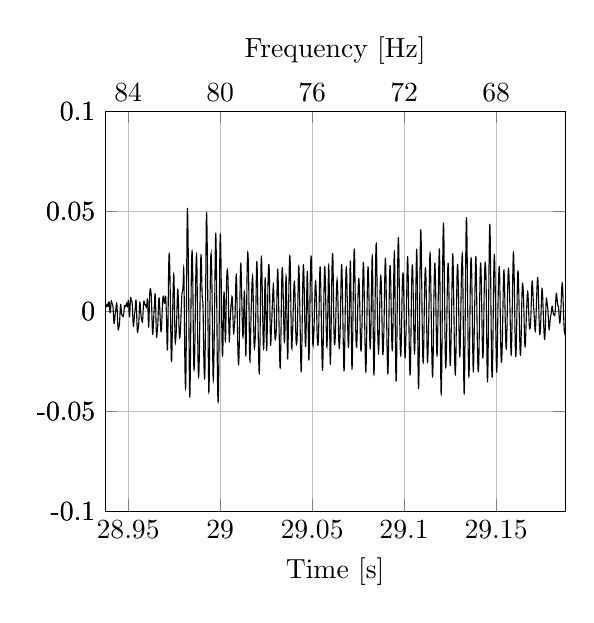
\begin{tikzpicture}


\begin{axis}[%
width=2.3in,
height=2in,
at={(1.011in,0.642in)},
scale only axis,
xmin=28.9375,
xmax=29.1875,
xtick={28.95, 29, 29.05,  29.1, 29.15},
xticklabels={84, 80, 76, 72, 68},
xmajorgrids,
ymin=-0.1,
ymax=0.1,
ymajorgrids,
scaled ticks=false,
ytick={-0.1, -0.05, 0,  0.05, 0.1},
yticklabels={-0.1, -0.05, 0,  0.05, 0.1},
axis x line*=top,
xlabel={Frequency [Hz]},
axis background/.style={fill=white}
]
\end{axis}

\begin{axis}[%
width=2.3in,
height=2in,
at={(1.011in,0.642in)},
scale only axis,
xmin=28.9375,
xmax=29.1875,
xmajorgrids,
ymin=-0.1,
ymax=0.1,
ymajorgrids,
scaled ticks=false,
ytick={-0.1, -0.05, 0,  0.05, 0.1},
yticklabels={-0.1, -0.05, 0,  0.05, 0.1},
xlabel={Time [s]},
axis background/.style={fill=white}
]
\addplot [color=black,solid,forget plot]
table[row sep=crcr]{%
	28.9374791666667	0.00120449066162109\\
	28.9375	0.0013422966003418\\
	28.9375208333333	0.00147902965545654\\
	28.9375416666667	0.00158834457397461\\
	28.9375625	0.00170481204986572\\
	28.9375833333333	0.00182092189788818\\
	28.9376041666667	0.00190639495849609\\
	28.937625	0.00197184085845947\\
	28.9376458333333	0.00206494331359863\\
	28.9376666666667	0.00211882591247559\\
	28.9376875	0.00217843055725098\\
	28.9377083333333	0.00219666957855225\\
	28.9377291666667	0.00223839282989502\\
	28.93775	0.00232481956481934\\
	28.9377708333333	0.00233364105224609\\
	28.9377916666667	0.00235855579376221\\
	28.9378125	0.00237452983856201\\
	28.9378333333333	0.00237023830413818\\
	28.9378541666667	0.00236904621124268\\
	28.937875	0.0023728609085083\\
	28.9378958333333	0.00235486030578613\\
	28.9379166666667	0.00235366821289063\\
	28.9379375	0.00235486030578613\\
	28.9379583333333	0.00233364105224609\\
	28.9379791666667	0.00234019756317139\\
	28.938	0.00231480598449707\\
	28.9380208333333	0.00231778621673584\\
	28.9380416666667	0.00233066082000732\\
	28.9380625	0.00229394435882568\\
	28.9380833333333	0.00233161449432373\\
	28.9381041666667	0.00232195854187012\\
	28.938125	0.00232744216918945\\
	28.9381458333333	0.00236666202545166\\
	28.9381666666667	0.00239074230194092\\
	28.9381875	0.0024111270904541\\
	28.9382083333333	0.00241708755493164\\
	28.9382291666667	0.00250089168548584\\
	28.93825	0.00255060195922852\\
	28.9382708333333	0.00261783599853516\\
	28.9382916666667	0.00265705585479736\\
	28.9383125	0.00270915031433105\\
	28.9383333333333	0.00275206565856934\\
	28.9383541666667	0.00282132625579834\\
	28.938375	0.00291812419891357\\
	28.9383958333333	0.00299406051635742\\
	28.9384166666667	0.00303125381469727\\
	28.9384375	0.00311172008514404\\
	28.9384583333333	0.00321066379547119\\
	28.9384791666667	0.0032811164855957\\
	28.9385	0.00332748889923096\\
	28.9385208333333	0.00336956977844238\\
	28.9385416666667	0.00345480442047119\\
	28.9385625	0.00349807739257813\\
	28.9385833333333	0.00352728366851807\\
	28.9386041666667	0.0035477876663208\\
	28.938625	0.0035707950592041\\
	28.9386458333333	0.00359570980072021\\
	28.9386666666667	0.0036003589630127\\
	28.9386875	0.00357067584991455\\
	28.9387083333333	0.00353062152862549\\
	28.9387291666667	0.00348305702209473\\
	28.93875	0.00348186492919922\\
	28.9387708333333	0.0034555196762085\\
	28.9387916666667	0.00335538387298584\\
	28.9388125	0.00326108932495117\\
	28.9388333333333	0.00318527221679688\\
	28.9388541666667	0.00317442417144775\\
	28.938875	0.00306880474090576\\
	28.9388958333333	0.00293564796447754\\
	28.9389166666667	0.00287473201751709\\
	28.9389375	0.00280296802520752\\
	28.9389583333333	0.00272119045257568\\
	28.9389791666667	0.00266194343566895\\
	28.939	0.00259816646575928\\
	28.9390208333333	0.0025409460067749\\
	28.9390416666667	0.00249350070953369\\
	28.9390625	0.00247383117675781\\
	28.9390833333333	0.00246036052703857\\
	28.9391041666667	0.00245332717895508\\
	28.939125	0.00244832038879395\\
	28.9391458333333	0.00248098373413086\\
	28.9391666666667	0.00252044200897217\\
	28.9391875	0.00253975391387939\\
	28.9392083333333	0.00264823436737061\\
	28.9392291666667	0.00271797180175781\\
	28.93925	0.00281059741973877\\
	28.9392708333333	0.00290811061859131\\
	28.9392916666667	0.00302028656005859\\
	28.9393125	0.00315308570861816\\
	28.9393333333333	0.00329148769378662\\
	28.9393541666667	0.00340831279754639\\
	28.939375	0.00356948375701904\\
	28.9393958333333	0.00372171401977539\\
	28.9394166666667	0.00384736061096191\\
	28.9394375	0.0039832592010498\\
	28.9394583333333	0.00412929058074951\\
	28.9394791666667	0.00424027442932129\\
	28.9395	0.00433218479156494\\
	28.9395208333333	0.00442314147949219\\
	28.9395416666667	0.00449824333190918\\
	28.9395625	0.00455284118652344\\
	28.9395833333333	0.00458669662475586\\
	28.9396041666667	0.0046314001083374\\
	28.939625	0.00459587574005127\\
	28.9396458333333	0.0045621395111084\\
	28.9396666666667	0.00453615188598633\\
	28.9396875	0.0044330358505249\\
	28.9397083333333	0.00432121753692627\\
	28.9397291666667	0.00419533252716064\\
	28.93975	0.00404250621795654\\
	28.9397708333333	0.00387072563171387\\
	28.9397916666667	0.00365662574768066\\
	28.9398125	0.003456711769104\\
	28.9398333333333	0.00322723388671875\\
	28.9398541666667	0.002982497215271\\
	28.939875	0.00272881984710693\\
	28.9398958333333	0.00249087810516357\\
	28.9399166666667	0.00224483013153076\\
	28.9399375	0.00196731090545654\\
	28.9399583333333	0.00170230865478516\\
	28.9399791666667	0.00142776966094971\\
	28.94	0.00115609169006348\\
	28.9400208333333	0.000885367393493652\\
	28.9400416666667	0.000633358955383301\\
	28.9400625	0.000411391258239746\\
	28.9400833333333	0.000180602073669434\\
	28.9401041666667	-8.34465026855469e-06\\
	28.940125	-0.000194072723388672\\
	28.9401458333333	-0.000409603118896484\\
	28.9401666666667	-0.000522017478942871\\
	28.9401875	-0.000576972961425781\\
	28.9402083333333	-0.000643014907836914\\
	28.9402291666667	-0.000677943229675293\\
	28.94025	-0.000661253929138184\\
	28.9402708333333	-0.000652074813842773\\
	28.9402916666667	-0.000607490539550781\\
	28.9403125	-0.000536084175109863\\
	28.9403333333333	-0.000380039215087891\\
	28.9403541666667	-0.000264167785644531\\
	28.940375	-0.00012516975402832\\
	28.9403958333333	1.87158584594727e-05\\
	28.9404166666667	0.000219106674194336\\
	28.9404375	0.000468611717224121\\
	28.9404583333333	0.000717759132385254\\
	28.9404791666667	0.00103902816772461\\
	28.9405	0.00130844116210938\\
	28.9405208333333	0.00157058238983154\\
	28.9405416666667	0.00185871124267578\\
	28.9405625	0.00217807292938232\\
	28.9405833333333	0.00246882438659668\\
	28.9406041666667	0.0027240514755249\\
	28.940625	0.00297737121582031\\
	28.9406458333333	0.00324654579162598\\
	28.9406666666667	0.00350058078765869\\
	28.9406875	0.00375759601593018\\
	28.9407083333333	0.0039670467376709\\
	28.9407291666667	0.00423252582550049\\
	28.94075	0.00441229343414307\\
	28.9407708333333	0.00458657741546631\\
	28.9407916666667	0.00479030609130859\\
	28.9408125	0.00493013858795166\\
	28.9408333333333	0.00502967834472656\\
	28.9408541666667	0.00513112545013428\\
	28.940875	0.00521993637084961\\
	28.9408958333333	0.00522971153259277\\
	28.9409166666667	0.00522172451019287\\
	28.9409375	0.00522911548614502\\
	28.9409583333333	0.00523996353149414\\
	28.9409791666667	0.0052112340927124\\
	28.941	0.00512528419494629\\
	28.9410208333333	0.00503182411193848\\
	28.9410416666667	0.00497424602508545\\
	28.9410625	0.00487077236175537\\
	28.9410833333333	0.00477099418640137\\
	28.9411041666667	0.00464916229248047\\
	28.941125	0.004547119140625\\
	28.9411458333333	0.00443184375762939\\
	28.9411666666667	0.00429177284240723\\
	28.9411875	0.00418353080749512\\
	28.9412083333333	0.00412440299987793\\
	28.9412291666667	0.00401580333709717\\
	28.94125	0.00392568111419678\\
	28.9412708333333	0.00388896465301514\\
	28.9412916666667	0.0037989616394043\\
	28.9413125	0.00372517108917236\\
	28.9413333333333	0.00367295742034912\\
	28.9413541666667	0.00364494323730469\\
	28.941375	0.00362873077392578\\
	28.9413958333333	0.00360417366027832\\
	28.9414166666667	0.00356161594390869\\
	28.9414375	0.00357687473297119\\
	28.9414583333333	0.00352346897125244\\
	28.9414791666667	0.00348567962646484\\
	28.9415	0.00347518920898438\\
	28.9415208333333	0.00347352027893066\\
	28.9415416666667	0.00342643260955811\\
	28.9415625	0.00337326526641846\\
	28.9415833333333	0.00334906578063965\\
	28.9416041666667	0.00328314304351807\\
	28.941625	0.00321304798126221\\
	28.9416458333333	0.00310385227203369\\
	28.9416666666667	0.0030217170715332\\
	28.9416875	0.00289404392242432\\
	28.9417083333333	0.00277328491210938\\
	28.9417291666667	0.00259971618652344\\
	28.94175	0.00243127346038818\\
	28.9417708333333	0.00223422050476074\\
	28.9417916666667	0.00204789638519287\\
	28.9418125	0.00179445743560791\\
	28.9418333333333	0.00156998634338379\\
	28.9418541666667	0.00131797790527344\\
	28.941875	0.00100135803222656\\
	28.9418958333333	0.000730276107788086\\
	28.9419166666667	0.000393033027648926\\
	28.9419375	4.80413436889648e-05\\
	28.9419583333333	-0.000273346900939941\\
	28.9419791666667	-0.000638008117675781\\
	28.942	-0.000986218452453613\\
	28.9420208333333	-0.0013500452041626\\
	28.9420416666667	-0.00172805786132813\\
	28.9420625	-0.00209999084472656\\
	28.9420833333333	-0.00245952606201172\\
	28.9421041666667	-0.00283920764923096\\
	28.942125	-0.00321090221405029\\
	28.9421458333333	-0.00355565547943115\\
	28.9421666666667	-0.00390529632568359\\
	28.9421875	-0.00425815582275391\\
	28.9422083333333	-0.00453579425811768\\
	28.9422291666667	-0.00481522083282471\\
	28.94225	-0.00510096549987793\\
	28.9422708333333	-0.00531721115112305\\
	28.9422916666667	-0.00551402568817139\\
	28.9423125	-0.00571227073669434\\
	28.9423333333333	-0.00587165355682373\\
	28.9423541666667	-0.006011962890625\\
	28.942375	-0.00609862804412842\\
	28.9423958333333	-0.00616216659545898\\
	28.9424166666667	-0.0061640739440918\\
	28.9424375	-0.00617873668670654\\
	28.9424583333333	-0.0061715841293335\\
	28.9424791666667	-0.00609982013702393\\
	28.9425	-0.00601935386657715\\
	28.9425208333333	-0.00593757629394531\\
	28.9425416666667	-0.00584173202514648\\
	28.9425625	-0.00566816329956055\\
	28.9425833333333	-0.00552630424499512\\
	28.9426041666667	-0.00535976886749268\\
	28.942625	-0.00518405437469482\\
	28.9426458333333	-0.00501167774200439\\
	28.9426666666667	-0.00480484962463379\\
	28.9426875	-0.00459206104278564\\
	28.9427083333333	-0.004372239112854\\
	28.9427291666667	-0.00415718555450439\\
	28.94275	-0.00394749641418457\\
	28.9427708333333	-0.00370919704437256\\
	28.9427916666667	-0.00349545478820801\\
	28.9428125	-0.00327563285827637\\
	28.9428333333333	-0.00306379795074463\\
	28.9428541666667	-0.00283503532409668\\
	28.942875	-0.00266897678375244\\
	28.9428958333333	-0.00242698192596436\\
	28.9429166666667	-0.00224006175994873\\
	28.9429375	-0.00203025341033936\\
	28.9429583333333	-0.00185549259185791\\
	28.9429791666667	-0.00171148777008057\\
	28.943	-0.00151622295379639\\
	28.9430208333333	-0.00136935710906982\\
	28.9430416666667	-0.00121152400970459\\
	28.9430625	-0.00106132030487061\\
	28.9430833333333	-0.000919103622436523\\
	28.9431041666667	-0.000782370567321777\\
	28.943125	-0.000638723373413086\\
	28.9431458333333	-0.000498175621032715\\
	28.9431666666667	-0.000345945358276367\\
	28.9431875	-0.000230789184570313\\
	28.9432083333333	-8.38041305541992e-05\\
	28.9432291666667	8.63075256347656e-05\\
	28.94325	0.00023949146270752\\
	28.9432708333333	0.000397205352783203\\
	28.9432916666667	0.000530004501342773\\
	28.9433125	0.000728845596313477\\
	28.9433333333333	0.000880002975463867\\
	28.9433541666667	0.00105178356170654\\
	28.943375	0.00125205516815186\\
	28.9433958333333	0.00144445896148682\\
	28.9434166666667	0.00165307521820068\\
	28.9434375	0.00179791450500488\\
	28.9434583333333	0.00201606750488281\\
	28.9434791666667	0.00223231315612793\\
	28.9435	0.00242531299591064\\
	28.9435208333333	0.00262200832366943\\
	28.9435416666667	0.00280725955963135\\
	28.9435625	0.00299155712127686\\
	28.9435833333333	0.00317680835723877\\
	28.9436041666667	0.00332033634185791\\
	28.943625	0.00349819660186768\\
	28.9436458333333	0.00365996360778809\\
	28.9436666666667	0.00376176834106445\\
	28.9436875	0.0038527250289917\\
	28.9437083333333	0.00394964218139648\\
	28.9437291666667	0.00402390956878662\\
	28.94375	0.00402307510375977\\
	28.9437708333333	0.0040431022644043\\
	28.9437916666667	0.00400960445404053\\
	28.9438125	0.00398123264312744\\
	28.9438333333333	0.00387287139892578\\
	28.9438541666667	0.00376808643341064\\
	28.943875	0.0036466121673584\\
	28.9438958333333	0.00343811511993408\\
	28.9439166666667	0.00322556495666504\\
	28.9439375	0.00299918651580811\\
	28.9439583333333	0.00274956226348877\\
	28.9439791666667	0.00238537788391113\\
	28.944	0.00204110145568848\\
	28.9440208333333	0.00170993804931641\\
	28.9440416666667	0.00127840042114258\\
	28.9440625	0.00086820125579834\\
	28.9440833333333	0.00043022632598877\\
	28.9441041666667	-4.25577163696289e-05\\
	28.944125	-0.000528573989868164\\
	28.9441458333333	-0.000995159149169922\\
	28.9441666666667	-0.00151360034942627\\
	28.9441875	-0.00202596187591553\\
	28.9442083333333	-0.00253725051879883\\
	28.9442291666667	-0.00308370590209961\\
	28.94425	-0.00356650352478027\\
	28.9442708333333	-0.00408291816711426\\
	28.9442916666667	-0.00460159778594971\\
	28.9443125	-0.00507307052612305\\
	28.9443333333333	-0.00550568103790283\\
	28.9443541666667	-0.00596094131469727\\
	28.944375	-0.00639355182647705\\
	28.9443958333333	-0.00678336620330811\\
	28.9444166666667	-0.00715458393096924\\
	28.9444375	-0.00749218463897705\\
	28.9444583333333	-0.00781965255737305\\
	28.9444791666667	-0.00808835029602051\\
	28.9445	-0.00832915306091309\\
	28.9445208333333	-0.00857234001159668\\
	28.9445416666667	-0.0087350606918335\\
	28.9445625	-0.00887703895568848\\
	28.9445833333333	-0.00901639461517334\\
	28.9446041666667	-0.00910532474517822\\
	28.944625	-0.00917530059814453\\
	28.9446458333333	-0.00921499729156494\\
	28.9446666666667	-0.00927221775054932\\
	28.9446875	-0.0092463493347168\\
	28.9447083333333	-0.00926792621612549\\
	28.9447291666667	-0.00922989845275879\\
	28.94475	-0.00919866561889648\\
	28.9447708333333	-0.00914144515991211\\
	28.9447916666667	-0.00907063484191895\\
	28.9448125	-0.00901293754577637\\
	28.9448333333333	-0.00892424583435059\\
	28.9448541666667	-0.00883769989013672\\
	28.944875	-0.00875723361968994\\
	28.9448958333333	-0.00870335102081299\\
	28.9449166666667	-0.0085904598236084\\
	28.9449375	-0.00850820541381836\\
	28.9449583333333	-0.00839269161224365\\
	28.9449791666667	-0.00831711292266846\\
	28.945	-0.0082094669342041\\
	28.9450208333333	-0.00813567638397217\\
	28.9450416666667	-0.00805056095123291\\
	28.9450625	-0.0079272985458374\\
	28.9450833333333	-0.00782966613769531\\
	28.9451041666667	-0.0077434778213501\\
	28.945125	-0.00762271881103516\\
	28.9451458333333	-0.00748217105865479\\
	28.9451666666667	-0.0074012279510498\\
	28.9451875	-0.00725114345550537\\
	28.9452083333333	-0.00711047649383545\\
	28.9452291666667	-0.00694930553436279\\
	28.94525	-0.0067903995513916\\
	28.9452708333333	-0.00657689571380615\\
	28.9452916666667	-0.00638699531555176\\
	28.9453125	-0.00614047050476074\\
	28.9453333333333	-0.00589501857757568\\
	28.9453541666667	-0.00564134120941162\\
	28.945375	-0.00533878803253174\\
	28.9453958333333	-0.0050283670425415\\
	28.9454166666667	-0.0046771764755249\\
	28.9454375	-0.0043487548828125\\
	28.9454583333333	-0.00397193431854248\\
	28.9454791666667	-0.00359225273132324\\
	28.9455	-0.00320053100585938\\
	28.9455208333333	-0.00277113914489746\\
	28.9455416666667	-0.00234317779541016\\
	28.9455625	-0.00193297863006592\\
	28.9455833333333	-0.00148999691009521\\
	28.9456041666667	-0.0010521411895752\\
	28.945625	-0.000657558441162109\\
	28.9456458333333	-0.000228643417358398\\
	28.9456666666667	0.000164389610290527\\
	28.9456875	0.000571966171264648\\
	28.9457083333333	0.000959157943725586\\
	28.9457291666667	0.0012742280960083\\
	28.94575	0.00164806842803955\\
	28.9457708333333	0.00197863578796387\\
	28.9457916666667	0.00224733352661133\\
	28.9458125	0.00248706340789795\\
	28.9458333333333	0.00269651412963867\\
	28.9458541666667	0.00291526317596436\\
	28.945875	0.00307631492614746\\
	28.9458958333333	0.00319766998291016\\
	28.9459166666667	0.00328361988067627\\
	28.9459375	0.00333547592163086\\
	28.9459583333333	0.0033566951751709\\
	28.9459791666667	0.00334405899047852\\
	28.946	0.00330209732055664\\
	28.9460208333333	0.00322556495666504\\
	28.9460416666667	0.00311374664306641\\
	28.9460625	0.00297248363494873\\
	28.9460833333333	0.00281548500061035\\
	28.9461041666667	0.00264823436737061\\
	28.946125	0.00243580341339111\\
	28.9461458333333	0.00223219394683838\\
	28.9461666666667	0.00200450420379639\\
	28.9461875	0.00174605846405029\\
	28.9462083333333	0.00149452686309814\\
	28.9462291666667	0.00123834609985352\\
	28.94625	0.000975608825683594\\
	28.9462708333333	0.000711798667907715\\
	28.9462916666667	0.000437259674072266\\
	28.9463125	0.000186920166015625\\
	28.9463333333333	-4.62532043457031e-05\\
	28.9463541666667	-0.000296592712402344\\
	28.946375	-0.000509381294250488\\
	28.9463958333333	-0.000693798065185547\\
	28.9464166666667	-0.000870347023010254\\
	28.9464375	-0.00106263160705566\\
	28.9464583333333	-0.00124084949493408\\
	28.9464791666667	-0.00135302543640137\\
	28.9465	-0.00150108337402344\\
	28.9465208333333	-0.00159585475921631\\
	28.9465416666667	-0.00174951553344727\\
	28.9465625	-0.00178027153015137\\
	28.9465833333333	-0.00185716152191162\\
	28.9466041666667	-0.00190210342407227\\
	28.946625	-0.00194311141967773\\
	28.9466458333333	-0.00195682048797607\\
	28.9466666666667	-0.00200092792510986\\
	28.9466875	-0.00200068950653076\\
	28.9467083333333	-0.00199317932128906\\
	28.9467291666667	-0.00199985504150391\\
	28.94675	-0.00198268890380859\\
	28.9467708333333	-0.00201892852783203\\
	28.9467916666667	-0.00195181369781494\\
	28.9468125	-0.00197136402130127\\
	28.9468333333333	-0.00197088718414307\\
	28.9468541666667	-0.00195300579071045\\
	28.946875	-0.0019221305847168\\
	28.9468958333333	-0.00193166732788086\\
	28.9469166666667	-0.00193977355957031\\
	28.9469375	-0.00197398662567139\\
	28.9469583333333	-0.00198137760162354\\
	28.9469791666667	-0.00202929973602295\\
	28.947	-0.00204813480377197\\
	28.9470208333333	-0.00205314159393311\\
	28.9470416666667	-0.0021357536315918\\
	28.9470625	-0.00214993953704834\\
	28.9470833333333	-0.0022275447845459\\
	28.9471041666667	-0.00226342678070068\\
	28.947125	-0.0023338794708252\\
	28.9471458333333	-0.0023953914642334\\
	28.9471666666667	-0.00243794918060303\\
	28.9471875	-0.00251471996307373\\
	28.9472083333333	-0.00256145000457764\\
	28.9472291666667	-0.00262069702148438\\
	28.94725	-0.00264477729797363\\
	28.9472708333333	-0.00268018245697021\\
	28.9472916666667	-0.00271868705749512\\
	28.9473125	-0.00275373458862305\\
	28.9473333333333	-0.0027240514755249\\
	28.9473541666667	-0.00271487236022949\\
	28.947375	-0.00269734859466553\\
	28.9473958333333	-0.00266361236572266\\
	28.9474166666667	-0.00259816646575928\\
	28.9474375	-0.00254809856414795\\
	28.9474583333333	-0.0024724006652832\\
	28.9474791666667	-0.00236475467681885\\
	28.9475	-0.00222373008728027\\
	28.9475208333333	-0.00209498405456543\\
	28.9475416666667	-0.00199651718139648\\
	28.9475625	-0.00181496143341064\\
	28.9475833333333	-0.00161874294281006\\
	28.9476041666667	-0.00142979621887207\\
	28.947625	-0.00125586986541748\\
	28.9476458333333	-0.00103628635406494\\
	28.9476666666667	-0.00085151195526123\\
	28.9476875	-0.000629663467407227\\
	28.9477083333333	-0.000427961349487305\\
	28.9477291666667	-0.000189900398254395\\
	28.94775	2.43186950683594e-05\\
	28.9477708333333	0.000212907791137695\\
	28.9477916666667	0.000438451766967773\\
	28.9478125	0.000701308250427246\\
	28.9478333333333	0.000888824462890625\\
	28.9478541666667	0.00107264518737793\\
	28.947875	0.00127303600311279\\
	28.9478958333333	0.00148415565490723\\
	28.9479166666667	0.00163650512695313\\
	28.9479375	0.00178205966949463\\
	28.9479583333333	0.0019611120223999\\
	28.9479791666667	0.00208234786987305\\
	28.948	0.0022122859954834\\
	28.9480208333333	0.00233030319213867\\
	28.9480416666667	0.00245213508605957\\
	28.9480625	0.00254130363464355\\
	28.9480833333333	0.00261390209197998\\
	28.9481041666667	0.00266730785369873\\
	28.948125	0.002768874168396\\
	28.9481458333333	0.00282394886016846\\
	28.9481666666667	0.00283098220825195\\
	28.9481875	0.00286483764648438\\
	28.9482083333333	0.00290322303771973\\
	28.9482291666667	0.00289678573608398\\
	28.94825	0.0028834342956543\\
	28.9482708333333	0.00288903713226318\\
	28.9482916666667	0.00288474559783936\\
	28.9483125	0.00286269187927246\\
	28.9483333333333	0.00282883644104004\\
	28.9483541666667	0.00279414653778076\\
	28.948375	0.00276303291320801\\
	28.9483958333333	0.00272870063781738\\
	28.9484166666667	0.00271797180175781\\
	28.9484375	0.00267577171325684\\
	28.9484583333333	0.00263571739196777\\
	28.9484791666667	0.00257432460784912\\
	28.9485	0.00260186195373535\\
	28.9485208333333	0.00261199474334717\\
	28.9485416666667	0.0025259256362915\\
	28.9485625	0.00253629684448242\\
	28.9485833333333	0.00254309177398682\\
	28.9486041666667	0.00254881381988525\\
	28.948625	0.00251924991607666\\
	28.9486458333333	0.00258731842041016\\
	28.9486666666667	0.0026010274887085\\
	28.9486875	0.00260651111602783\\
	28.9487083333333	0.00261986255645752\\
	28.9487291666667	0.00269746780395508\\
	28.94875	0.00275719165802002\\
	28.9487708333333	0.00278258323669434\\
	28.9487916666667	0.00282752513885498\\
	28.9488125	0.00287473201751709\\
	28.9488333333333	0.00293600559234619\\
	28.9488541666667	0.00301527976989746\\
	28.948875	0.0030893087387085\\
	28.9488958333333	0.00317025184631348\\
	28.9489166666667	0.00324559211730957\\
	28.9489375	0.00328946113586426\\
	28.9489583333333	0.00333797931671143\\
	28.9489791666667	0.00340175628662109\\
	28.949	0.00345754623413086\\
	28.9490208333333	0.00350940227508545\\
	28.9490416666667	0.00359416007995605\\
	28.9490625	0.00362908840179443\\
	28.9490833333333	0.00361824035644531\\
	28.9491041666667	0.0036015510559082\\
	28.949125	0.00365960597991943\\
	28.9491458333333	0.00370883941650391\\
	28.9491666666667	0.00361740589141846\\
	28.9491875	0.00354647636413574\\
	28.9492083333333	0.00355947017669678\\
	28.9492291666667	0.00348484516143799\\
	28.94925	0.00344514846801758\\
	28.9492708333333	0.00336253643035889\\
	28.9492916666667	0.00326979160308838\\
	28.9493125	0.00314474105834961\\
	28.9493333333333	0.00303030014038086\\
	28.9493541666667	0.00299572944641113\\
	28.949375	0.00288474559783936\\
	28.9493958333333	0.00273466110229492\\
	28.9494166666667	0.00265610218048096\\
	28.9494375	0.00257062911987305\\
	28.9494583333333	0.00245749950408936\\
	28.9494791666667	0.00238919258117676\\
	28.9495	0.00232481956481934\\
	28.9495208333333	0.00229990482330322\\
	28.9495416666667	0.00223338603973389\\
	28.9495625	0.002205491065979\\
	28.9495833333333	0.00222384929656982\\
	28.9496041666667	0.00224018096923828\\
	28.949625	0.00226807594299316\\
	28.9496458333333	0.002349853515625\\
	28.9496666666667	0.00245094299316406\\
	28.9496875	0.00250637531280518\\
	28.9497083333333	0.0025869607925415\\
	28.9497291666667	0.00275886058807373\\
	28.94975	0.00294363498687744\\
	28.9497708333333	0.00306534767150879\\
	28.9497916666667	0.00320351123809814\\
	28.9498125	0.00345981121063232\\
	28.9498333333333	0.00364840030670166\\
	28.9498541666667	0.00382018089294434\\
	28.949875	0.00399625301361084\\
	28.9498958333333	0.00420570373535156\\
	28.9499166666667	0.00439226627349854\\
	28.9499375	0.00453698635101318\\
	28.9499583333333	0.0047307014465332\\
	28.9499791666667	0.00490379333496094\\
	28.95	0.00499629974365234\\
	28.9500208333333	0.00507068634033203\\
	28.9500416666667	0.00517380237579346\\
	28.9500625	0.00527513027191162\\
	28.9500833333333	0.00526750087738037\\
	28.9501041666667	0.00522792339324951\\
	28.950125	0.00524055957794189\\
	28.9501458333333	0.00517702102661133\\
	28.9501666666667	0.00502884387969971\\
	28.9501875	0.00488781929016113\\
	28.9502083333333	0.00475656986236572\\
	28.9502291666667	0.00458204746246338\\
	28.95025	0.00433135032653809\\
	28.9502708333333	0.00405228137969971\\
	28.9502916666667	0.00383269786834717\\
	28.9503125	0.00350522994995117\\
	28.9503333333333	0.00316107273101807\\
	28.9503541666667	0.00278890132904053\\
	28.950375	0.00247848033905029\\
	28.9503958333333	0.00213134288787842\\
	28.9504166666667	0.0016934871673584\\
	28.9504375	0.00128757953643799\\
	28.9504583333333	0.000902414321899414\\
	28.9504791666667	0.000477790832519531\\
	28.9505	3.38554382324219e-05\\
	28.9505208333333	-0.000324130058288574\\
	28.9505416666667	-0.000696778297424316\\
	28.9505625	-0.00110518932342529\\
	28.9505833333333	-0.00148618221282959\\
	28.9506041666667	-0.0017240047454834\\
	28.950625	-0.00196230411529541\\
	28.9506458333333	-0.00223922729492188\\
	28.9506666666667	-0.00240206718444824\\
	28.9506875	-0.00247740745544434\\
	28.9507083333333	-0.00260722637176514\\
	28.9507291666667	-0.00270664691925049\\
	28.95075	-0.00269615650177002\\
	28.9507708333333	-0.00262069702148438\\
	28.9507916666667	-0.00257313251495361\\
	28.9508125	-0.0025097131729126\\
	28.9508333333333	-0.00235104560852051\\
	28.9508541666667	-0.00208103656768799\\
	28.950875	-0.00179779529571533\\
	28.9508958333333	-0.00150954723358154\\
	28.9509166666667	-0.00117194652557373\\
	28.9509375	-0.000782370567321777\\
	28.9509583333333	-0.00044858455657959\\
	28.9509791666667	-8.34465026855469e-05\\
	28.951	0.000378012657165527\\
	28.9510208333333	0.000835776329040527\\
	28.9510416666667	0.00127923488616943\\
	28.9510625	0.00171661376953125\\
	28.9510833333333	0.00211620330810547\\
	28.9511041666667	0.00249087810516357\\
	28.951125	0.00293815135955811\\
	28.9511458333333	0.00336539745330811\\
	28.9511666666667	0.00378096103668213\\
	28.9511875	0.00420570373535156\\
	28.9512083333333	0.004599928855896\\
	28.9512291666667	0.00494003295898438\\
	28.95125	0.00526010990142822\\
	28.9512708333333	0.00555706024169922\\
	28.9512916666667	0.00581920146942139\\
	28.9513125	0.00606405735015869\\
	28.9513333333333	0.0062861442565918\\
	28.9513541666667	0.00645327568054199\\
	28.951375	0.00657689571380615\\
	28.9513958333333	0.00669670104980469\\
	28.9514166666667	0.00680875778198242\\
	28.9514375	0.00682854652404785\\
	28.9514583333333	0.00684773921966553\\
	28.9514791666667	0.00681555271148682\\
	28.9515	0.00680291652679443\\
	28.9515208333333	0.00669407844543457\\
	28.9515416666667	0.00658977031707764\\
	28.9515625	0.00653398036956787\\
	28.9515833333333	0.00641906261444092\\
	28.9516041666667	0.00633645057678223\\
	28.951625	0.0062251091003418\\
	28.9516458333333	0.00611782073974609\\
	28.9516666666667	0.00599849224090576\\
	28.9516875	0.00585758686065674\\
	28.9517083333333	0.00576698780059814\\
	28.9517291666667	0.00570058822631836\\
	28.95175	0.00557601451873779\\
	28.9517708333333	0.00548863410949707\\
	28.9517916666667	0.00545024871826172\\
	28.9518125	0.00538110733032227\\
	28.9518333333333	0.0052955150604248\\
	28.9518541666667	0.0052649974822998\\
	28.951875	0.00523805618286133\\
	28.9518958333333	0.00520634651184082\\
	28.9519166666667	0.0051729679107666\\
	28.9519375	0.00515663623809814\\
	28.9519583333333	0.00512909889221191\\
	28.9519791666667	0.00505387783050537\\
	28.952	0.00503396987915039\\
	28.9520208333333	0.0050126314163208\\
	28.9520416666667	0.00497937202453613\\
	28.9520625	0.00488507747650146\\
	28.9520833333333	0.00477564334869385\\
	28.9521041666667	0.00469386577606201\\
	28.952125	0.00460553169250488\\
	28.9521458333333	0.00447690486907959\\
	28.9521666666667	0.00430679321289063\\
	28.9521875	0.00413095951080322\\
	28.9522083333333	0.00396382808685303\\
	28.9522291666667	0.00372219085693359\\
	28.95225	0.00348925590515137\\
	28.9522708333333	0.00323283672332764\\
	28.9522916666667	0.00292778015136719\\
	28.9523125	0.00257265567779541\\
	28.9523333333333	0.00225222110748291\\
	28.9523541666667	0.00188350677490234\\
	28.952375	0.00146079063415527\\
	28.9523958333333	0.00111985206604004\\
	28.9524166666667	0.000669598579406738\\
	28.9524375	0.000219464302062988\\
	28.9524583333333	-0.000203490257263184\\
	28.9524791666667	-0.000688910484313965\\
	28.9525	-0.00115406513214111\\
	28.9525208333333	-0.00164473056793213\\
	28.9525416666667	-0.00214004516601563\\
	28.9525625	-0.00266695022583008\\
	28.9525833333333	-0.00313663482666016\\
	28.9526041666667	-0.00356113910675049\\
	28.952625	-0.00401782989501953\\
	28.9526458333333	-0.00445592403411865\\
	28.9526666666667	-0.00490152835845947\\
	28.9526875	-0.00530540943145752\\
	28.9527083333333	-0.00565338134765625\\
	28.9527291666667	-0.0059959888458252\\
	28.95275	-0.00635015964508057\\
	28.9527708333333	-0.00661516189575195\\
	28.9527916666667	-0.00686180591583252\\
	28.9528125	-0.00709497928619385\\
	28.9528333333333	-0.00728070735931396\\
	28.9528541666667	-0.00741219520568848\\
	28.952875	-0.00749480724334717\\
	28.9528958333333	-0.00756931304931641\\
	28.9529166666667	-0.00758779048919678\\
	28.9529375	-0.00757312774658203\\
	28.9529583333333	-0.00751519203186035\\
	28.9529791666667	-0.00745391845703125\\
	28.953	-0.00731074810028076\\
	28.9530208333333	-0.00720894336700439\\
	28.9530416666667	-0.00704288482666016\\
	28.9530625	-0.00687050819396973\\
	28.9530833333333	-0.00668728351593018\\
	28.9531041666667	-0.00647926330566406\\
	28.953125	-0.00625467300415039\\
	28.9531458333333	-0.00600981712341309\\
	28.9531666666667	-0.00573980808258057\\
	28.9531875	-0.00549042224884033\\
	28.9532083333333	-0.0052182674407959\\
	28.9532291666667	-0.00494956970214844\\
	28.95325	-0.00468552112579346\\
	28.9532708333333	-0.00440812110900879\\
	28.9532916666667	-0.00417304039001465\\
	28.9533125	-0.00392496585845947\\
	28.9533333333333	-0.00367546081542969\\
	28.9533541666667	-0.00341963768005371\\
	28.953375	-0.00317132472991943\\
	28.9533958333333	-0.00293517112731934\\
	28.9534166666667	-0.00268399715423584\\
	28.9534375	-0.00247335433959961\\
	28.9534583333333	-0.00228261947631836\\
	28.9534791666667	-0.00204145908355713\\
	28.9535	-0.00187921524047852\\
	28.9535208333333	-0.00170278549194336\\
	28.9535416666667	-0.00151956081390381\\
	28.9535625	-0.00134849548339844\\
	28.9535833333333	-0.00116229057312012\\
	28.9536041666667	-0.00100100040435791\\
	28.953625	-0.000794291496276855\\
	28.9536458333333	-0.000609517097473145\\
	28.9536666666667	-0.000457167625427246\\
	28.9536875	-0.000290870666503906\\
	28.9537083333333	-6.79492950439453e-05\\
	28.9537291666667	0.000105500221252441\\
	28.95375	0.000274181365966797\\
	28.9537708333333	0.000500321388244629\\
	28.9537916666667	0.000700950622558594\\
	28.9538125	0.000948309898376465\\
	28.9538333333333	0.00116086006164551\\
	28.9538541666667	0.0013805627822876\\
	28.953875	0.00164890289306641\\
	28.9538958333333	0.00190436840057373\\
	28.9539166666667	0.00211906433105469\\
	28.9539375	0.00242495536804199\\
	28.9539583333333	0.00268375873565674\\
	28.9539791666667	0.00295066833496094\\
	28.954	0.00319314002990723\\
	28.9540208333333	0.00344312191009521\\
	28.9540416666667	0.00373101234436035\\
	28.9540625	0.00397837162017822\\
	28.9540833333333	0.00425004959106445\\
	28.9541041666667	0.00446522235870361\\
	28.954125	0.0046539306640625\\
	28.9541458333333	0.0048515796661377\\
	28.9541666666667	0.00503635406494141\\
	28.9541875	0.00519454479217529\\
	28.9542083333333	0.00532019138336182\\
	28.9542291666667	0.00537395477294922\\
	28.95425	0.00546491146087646\\
	28.9542708333333	0.00549256801605225\\
	28.9542916666667	0.00544416904449463\\
	28.9543125	0.00538980960845947\\
	28.9543333333333	0.00531816482543945\\
	28.9543541666667	0.00517880916595459\\
	28.954375	0.0049821138381958\\
	28.9543958333333	0.00475597381591797\\
	28.9544166666667	0.00447738170623779\\
	28.9544375	0.00416076183319092\\
	28.9544583333333	0.00379776954650879\\
	28.9544791666667	0.00340592861175537\\
	28.9545	0.00294911861419678\\
	28.9545208333333	0.00252604484558105\\
	28.9545416666667	0.00204122066497803\\
	28.9545625	0.00148046016693115\\
	28.9545833333333	0.000900387763977051\\
	28.9546041666667	0.000314235687255859\\
	28.954625	-0.000279426574707031\\
	28.9546458333333	-0.000893354415893555\\
	28.9546666666667	-0.00152122974395752\\
	28.9546875	-0.00219964981079102\\
	28.9547083333333	-0.00283873081207275\\
	28.9547291666667	-0.0034942626953125\\
	28.95475	-0.00412964820861816\\
	28.9547708333333	-0.00474798679351807\\
	28.9547916666667	-0.00536942481994629\\
	28.9548125	-0.00594055652618408\\
	28.9548333333333	-0.00648868083953857\\
	28.9548541666667	-0.00704109668731689\\
	28.954875	-0.00754189491271973\\
	28.9548958333333	-0.00797832012176514\\
	28.9549166666667	-0.00843691825866699\\
	28.9549375	-0.00882446765899658\\
	28.9549583333333	-0.00917530059814453\\
	28.9549791666667	-0.00946581363677979\\
	28.955	-0.00973606109619141\\
	28.9550208333333	-0.00999271869659424\\
	28.9550416666667	-0.0101704597473145\\
	28.9550625	-0.0103230476379395\\
	28.9550833333333	-0.0104254484176636\\
	28.9551041666667	-0.0105032920837402\\
	28.955125	-0.0105493068695068\\
	28.9551458333333	-0.0105750560760498\\
	28.9551666666667	-0.0105768442153931\\
	28.9551875	-0.0105404853820801\\
	28.9552083333333	-0.0104724168777466\\
	28.9552291666667	-0.0103836059570313\\
	28.95525	-0.010285496711731\\
	28.9552708333333	-0.0101571083068848\\
	28.9552916666667	-0.0100215673446655\\
	28.9553125	-0.00990748405456543\\
	28.9553333333333	-0.00978660583496094\\
	28.9553541666667	-0.00964224338531494\\
	28.955375	-0.0095217227935791\\
	28.9553958333333	-0.00938808917999268\\
	28.9554166666667	-0.0092320442199707\\
	28.9554375	-0.00913023948669434\\
	28.9554583333333	-0.00894427299499512\\
	28.9554791666667	-0.00882101058959961\\
	28.9555	-0.0086979866027832\\
	28.9555208333333	-0.00857293605804443\\
	28.9555416666667	-0.00847065448760986\\
	28.9555625	-0.00832951068878174\\
	28.9555833333333	-0.0082094669342041\\
	28.9556041666667	-0.00808465480804443\\
	28.955625	-0.00793445110321045\\
	28.9556458333333	-0.00778770446777344\\
	28.9556666666667	-0.0076291561126709\\
	28.9556875	-0.00744998455047607\\
	28.9557083333333	-0.00727570056915283\\
	28.9557291666667	-0.00702822208404541\\
	28.95575	-0.00678634643554688\\
	28.9557708333333	-0.00655519962310791\\
	28.9557916666667	-0.00625503063201904\\
	28.9558125	-0.00593018531799316\\
	28.9558333333333	-0.00559592247009277\\
	28.9558541666667	-0.00524747371673584\\
	28.955875	-0.00481438636779785\\
	28.9558958333333	-0.0044022798538208\\
	28.9559166666667	-0.0039752721786499\\
	28.9559375	-0.00349390506744385\\
	28.9559583333333	-0.00299704074859619\\
	28.9559791666667	-0.00252139568328857\\
	28.956	-0.00204360485076904\\
	28.9560208333333	-0.00151491165161133\\
	28.9560416666667	-0.00101673603057861\\
	28.9560625	-0.000505208969116211\\
	28.9560833333333	-7.15255737304688e-07\\
	28.9561041666667	0.000502347946166992\\
	28.956125	0.000982284545898438\\
	28.9561458333333	0.00147163867950439\\
	28.9561666666667	0.00189208984375\\
	28.9561875	0.00230145454406738\\
	28.9562083333333	0.00271952152252197\\
	28.9562291666667	0.00310266017913818\\
	28.95625	0.00342249870300293\\
	28.9562708333333	0.00370335578918457\\
	28.9562916666667	0.00393462181091309\\
	28.9563125	0.00415194034576416\\
	28.9563333333333	0.00431013107299805\\
	28.9563541666667	0.00444197654724121\\
	28.956375	0.00454044342041016\\
	28.9563958333333	0.00458753108978271\\
	28.9564166666667	0.0045846700668335\\
	28.9564375	0.00454378128051758\\
	28.9564583333333	0.00447869300842285\\
	28.9564791666667	0.00437462329864502\\
	28.9565	0.00427126884460449\\
	28.9565208333333	0.00410723686218262\\
	28.9565416666667	0.00391364097595215\\
	28.9565625	0.00366950035095215\\
	28.9565833333333	0.00344395637512207\\
	28.9566041666667	0.00315606594085693\\
	28.956625	0.0028681755065918\\
	28.9566458333333	0.00257217884063721\\
	28.9566666666667	0.00225400924682617\\
	28.9566875	0.00198066234588623\\
	28.9567083333333	0.00165057182312012\\
	28.9567291666667	0.00133812427520752\\
	28.95675	0.00105643272399902\\
	28.9567708333333	0.000751376152038574\\
	28.9567916666667	0.000424861907958984\\
	28.9568125	0.000171065330505371\\
	28.9568333333333	-9.0479850769043e-05\\
	28.9568541666667	-0.000412583351135254\\
	28.956875	-0.000677227973937988\\
	28.9568958333333	-0.000899434089660645\\
	28.9569166666667	-0.00112056732177734\\
	28.9569375	-0.00137567520141602\\
	28.9569583333333	-0.00157546997070313\\
	28.9569791666667	-0.00175034999847412\\
	28.957	-0.00192892551422119\\
	28.9570208333333	-0.00210666656494141\\
	28.9570416666667	-0.00226378440856934\\
	28.9570625	-0.00239062309265137\\
	28.9570833333333	-0.00253975391387939\\
	28.9571041666667	-0.00269770622253418\\
	28.957125	-0.00281667709350586\\
	28.9571458333333	-0.0028921365737915\\
	28.9571666666667	-0.00301814079284668\\
	28.9571875	-0.00316214561462402\\
	28.9572083333333	-0.00325405597686768\\
	28.9572291666667	-0.00332438945770264\\
	28.95725	-0.00347423553466797\\
	28.9572708333333	-0.00358736515045166\\
	28.9572916666667	-0.00364816188812256\\
	28.9573125	-0.00376880168914795\\
	28.9573333333333	-0.00388860702514648\\
	28.9573541666667	-0.00401592254638672\\
	28.957375	-0.00411760807037354\\
	28.9573958333333	-0.00422906875610352\\
	28.9574166666667	-0.00434303283691406\\
	28.9574375	-0.00446224212646484\\
	28.9574583333333	-0.00459122657775879\\
	28.9574791666667	-0.00470340251922607\\
	28.9575	-0.00483143329620361\\
	28.9575208333333	-0.00491082668304443\\
	28.9575416666667	-0.00500977039337158\\
	28.9575625	-0.00514519214630127\\
	28.9575833333333	-0.0052182674407959\\
	28.9576041666667	-0.00528013706207275\\
	28.957625	-0.00533974170684814\\
	28.9576458333333	-0.00541150569915771\\
	28.9576666666667	-0.0054318904876709\\
	28.9576875	-0.00544106960296631\\
	28.9577083333333	-0.00546121597290039\\
	28.9577291666667	-0.00540852546691895\\
	28.95775	-0.00538194179534912\\
	28.9577708333333	-0.0053030252456665\\
	28.9577916666667	-0.00520288944244385\\
	28.9578125	-0.00511598587036133\\
	28.9578333333333	-0.00496828556060791\\
	28.9578541666667	-0.00479567050933838\\
	28.957875	-0.00462913513183594\\
	28.9578958333333	-0.00439846515655518\\
	28.9579166666667	-0.00417149066925049\\
	28.9579375	-0.00386989116668701\\
	28.9579583333333	-0.00359725952148438\\
	28.9579791666667	-0.00328981876373291\\
	28.958	-0.0029522180557251\\
	28.9580208333333	-0.00262069702148438\\
	28.9580416666667	-0.00224769115447998\\
	28.9580625	-0.00188589096069336\\
	28.9580833333333	-0.0014883279800415\\
	28.9581041666667	-0.00112724304199219\\
	28.958125	-0.000753998756408691\\
	28.9581458333333	-0.000306248664855957\\
	28.9581666666667	8.85725021362305e-05\\
	28.9581875	0.000467658042907715\\
	28.9582083333333	0.000868678092956543\\
	28.9582291666667	0.00126349925994873\\
	28.95825	0.00159382820129395\\
	28.9582708333333	0.00193023681640625\\
	28.9582916666667	0.0022960901260376\\
	28.9583125	0.00263822078704834\\
	28.9583333333333	0.00293898582458496\\
	28.9583541666667	0.00319647789001465\\
	28.958375	0.00343501567840576\\
	28.9583958333333	0.00368666648864746\\
	28.9584166666667	0.0039290189743042\\
	28.9584375	0.00411438941955566\\
	28.9584583333333	0.00428915023803711\\
	28.9584791666667	0.00444447994232178\\
	28.9585	0.00455582141876221\\
	28.9585208333333	0.00466132164001465\\
	28.9585416666667	0.00477266311645508\\
	28.9585625	0.00482368469238281\\
	28.9585833333333	0.00485706329345703\\
	28.9586041666667	0.00491297245025635\\
	28.958625	0.00495719909667969\\
	28.9586458333333	0.00490915775299072\\
	28.9586666666667	0.00486946105957031\\
	28.9586875	0.00485026836395264\\
	28.9587083333333	0.00480246543884277\\
	28.9587291666667	0.00474405288696289\\
	28.95875	0.00468635559082031\\
	28.9587708333333	0.00462841987609863\\
	28.9587916666667	0.00449824333190918\\
	28.9588125	0.00438845157623291\\
	28.9588333333333	0.00435793399810791\\
	28.9588541666667	0.00428080558776855\\
	28.958875	0.0041424036026001\\
	28.9588958333333	0.00405645370483398\\
	28.9589166666667	0.00400471687316895\\
	28.9589375	0.00390815734863281\\
	28.9589583333333	0.00382733345031738\\
	28.9589791666667	0.00376176834106445\\
	28.959	0.00368845462799072\\
	28.9590208333333	0.00362837314605713\\
	28.9590416666667	0.00353908538818359\\
	28.9590625	0.00352597236633301\\
	28.9590833333333	0.00348150730133057\\
	28.9591041666667	0.00338888168334961\\
	28.959125	0.00334370136260986\\
	28.9591458333333	0.00332820415496826\\
	28.9591666666667	0.00326156616210938\\
	28.9591875	0.00322854518890381\\
	28.9592083333333	0.00319218635559082\\
	28.9592291666667	0.00316357612609863\\
	28.95925	0.0031430721282959\\
	28.9592708333333	0.00309181213378906\\
	28.9592916666667	0.00307798385620117\\
	28.9593125	0.00307083129882813\\
	28.9593333333333	0.00307929515838623\\
	28.9593541666667	0.00302028656005859\\
	28.959375	0.00298082828521729\\
	28.9593958333333	0.00300610065460205\\
	28.9594166666667	0.00300836563110352\\
	28.9594375	0.00296783447265625\\
	28.9594583333333	0.00297856330871582\\
	28.9594791666667	0.00301039218902588\\
	28.9595	0.00296151638031006\\
	28.9595208333333	0.00294613838195801\\
	28.9595416666667	0.00297081470489502\\
	28.9595625	0.00295579433441162\\
	28.9595833333333	0.00286734104156494\\
	28.9596041666667	0.0028759241104126\\
	28.959625	0.00288176536560059\\
	28.9596458333333	0.00281000137329102\\
	28.9596666666667	0.00275087356567383\\
	28.9596875	0.00270700454711914\\
	28.9597083333333	0.00270462036132813\\
	28.9597291666667	0.0026094913482666\\
	28.95975	0.00251424312591553\\
	28.9597708333333	0.00248515605926514\\
	28.9597916666667	0.00244176387786865\\
	28.9598125	0.00230515003204346\\
	28.9598333333333	0.00226759910583496\\
	28.9598541666667	0.00228989124298096\\
	28.959875	0.00221312046051025\\
	28.9598958333333	0.00210249423980713\\
	28.9599166666667	0.00208449363708496\\
	28.9599375	0.0022047758102417\\
	28.9599583333333	0.00214290618896484\\
	28.9599791666667	0.00208067893981934\\
	28.96	0.00213503837585449\\
	28.9600208333333	0.00225937366485596\\
	28.9600416666667	0.00232577323913574\\
	28.9600625	0.00237166881561279\\
	28.9600833333333	0.00248968601226807\\
	28.9601041666667	0.00265204906463623\\
	28.960125	0.00277423858642578\\
	28.9601458333333	0.00292432308197021\\
	28.9601666666667	0.00315630435943604\\
	28.9601875	0.00336587429046631\\
	28.9602083333333	0.00355863571166992\\
	28.9602291666667	0.00375306606292725\\
	28.96025	0.0039900541305542\\
	28.9602708333333	0.00423324108123779\\
	28.9602916666667	0.00445401668548584\\
	28.9603125	0.00469350814819336\\
	28.9603333333333	0.00496053695678711\\
	28.9603541666667	0.00517582893371582\\
	28.960375	0.00533473491668701\\
	28.9603958333333	0.00551259517669678\\
	28.9604166666667	0.00574064254760742\\
	28.9604375	0.0058741569519043\\
	28.9604583333333	0.00594353675842285\\
	28.9604791666667	0.0060044527053833\\
	28.9605	0.00608706474304199\\
	28.9605208333333	0.00607001781463623\\
	28.9605416666667	0.00602066516876221\\
	28.9605625	0.00594222545623779\\
	28.9605833333333	0.00582301616668701\\
	28.9606041666667	0.00564396381378174\\
	28.960625	0.00539326667785645\\
	28.9606458333333	0.00517582893371582\\
	28.9606666666667	0.00482869148254395\\
	28.9606875	0.0044102668762207\\
	28.9607083333333	0.00404214859008789\\
	28.9607291666667	0.00359189510345459\\
	28.96075	0.00300586223602295\\
	28.9607708333333	0.00237274169921875\\
	28.9607916666667	0.00178325176239014\\
	28.9608125	0.00113105773925781\\
	28.9608333333333	0.000365495681762695\\
	28.9608541666667	-0.000380992889404297\\
	28.960875	-0.00107312202453613\\
	28.9608958333333	-0.0018237829208374\\
	28.9609166666667	-0.00260269641876221\\
	28.9609375	-0.00324511528015137\\
	28.9609583333333	-0.00386106967926025\\
	28.9609791666667	-0.0044701099395752\\
	28.961	-0.00507402420043945\\
	28.9610208333333	-0.0055617094039917\\
	28.9610416666667	-0.00603234767913818\\
	28.9610625	-0.006522536277771\\
	28.9610833333333	-0.00686502456665039\\
	28.9611041666667	-0.00710511207580566\\
	28.961125	-0.00736713409423828\\
	28.9611458333333	-0.00761115550994873\\
	28.9611666666667	-0.00773429870605469\\
	28.9611875	-0.00770509243011475\\
	28.9612083333333	-0.00755345821380615\\
	28.9612291666667	-0.00736665725708008\\
	28.96125	-0.00708878040313721\\
	28.9612708333333	-0.00673317909240723\\
	28.9612916666667	-0.00633609294891357\\
	28.9613125	-0.00583922863006592\\
	28.9613333333333	-0.00528120994567871\\
	28.9613541666667	-0.0047447681427002\\
	28.961375	-0.00417983531951904\\
	28.9613958333333	-0.00353050231933594\\
	28.9614166666667	-0.00286877155303955\\
	28.9614375	-0.00218379497528076\\
	28.9614583333333	-0.00142109394073486\\
	28.9614791666667	-0.000641703605651855\\
	28.9615	9.97781753540039e-05\\
	28.9615208333333	0.000829935073852539\\
	28.9615416666667	0.00164186954498291\\
	28.9615625	0.00244879722595215\\
	28.9615833333333	0.00325644016265869\\
	28.9616041666667	0.00396919250488281\\
	28.961625	0.00461471080780029\\
	28.9616458333333	0.00522804260253906\\
	28.9616666666667	0.00587832927703857\\
	28.9616875	0.00651669502258301\\
	28.9617083333333	0.00711798667907715\\
	28.9617291666667	0.0077364444732666\\
	28.96175	0.00827920436859131\\
	28.9617708333333	0.00874865055084229\\
	28.9617916666667	0.00913190841674805\\
	28.9618125	0.00951623916625977\\
	28.9618333333333	0.00974369049072266\\
	28.9618541666667	0.0100182294845581\\
	28.961875	0.0102889537811279\\
	28.9618958333333	0.0104821920394897\\
	28.9619166666667	0.0106514692306519\\
	28.9619375	0.0107780694961548\\
	28.9619583333333	0.0109632015228271\\
	28.9619791666667	0.0110411643981934\\
	28.962	0.0110743045806885\\
	28.9620208333333	0.0110816955566406\\
	28.9620416666667	0.0111067295074463\\
	28.9620625	0.0110859870910645\\
	28.9620833333333	0.0110983848571777\\
	28.9621041666667	0.0110651254653931\\
	28.962125	0.0109924077987671\\
	28.9621458333333	0.0109944343566895\\
	28.9621666666667	0.0109552145004272\\
	28.9621875	0.0109134912490845\\
	28.9622083333333	0.0108917951583862\\
	28.9622291666667	0.010913610458374\\
	28.96225	0.0108722448348999\\
	28.9622708333333	0.010759711265564\\
	28.9622916666667	0.0106019973754883\\
	28.9623125	0.0104871988296509\\
	28.9623333333333	0.0103648900985718\\
	28.9623541666667	0.0102463960647583\\
	28.962375	0.0101308822631836\\
	28.9623958333333	0.0099644660949707\\
	28.9624166666667	0.00979447364807129\\
	28.9624375	0.00957882404327393\\
	28.9624583333333	0.00943195819854736\\
	28.9624791666667	0.00923633575439453\\
	28.9625	0.00898420810699463\\
	28.9625208333333	0.00874018669128418\\
	28.9625416666667	0.00848448276519775\\
	28.9625625	0.00819408893585205\\
	28.9625833333333	0.00786113739013672\\
	28.9626041666667	0.00750446319580078\\
	28.962625	0.0071481466293335\\
	28.9626458333333	0.00675618648529053\\
	28.9626666666667	0.00633704662322998\\
	28.9626875	0.00586175918579102\\
	28.9627083333333	0.00536429882049561\\
	28.9627291666667	0.00485575199127197\\
	28.96275	0.00428462028503418\\
	28.9627708333333	0.00372755527496338\\
	28.9627916666667	0.0031510591506958\\
	28.9628125	0.00251221656799316\\
	28.9628333333333	0.00184381008148193\\
	28.9628541666667	0.00115585327148438\\
	28.962875	0.000433921813964844\\
	28.9628958333333	-0.000317096710205078\\
	28.9629166666667	-0.00104808807373047\\
	28.9629375	-0.00179862976074219\\
	28.9629583333333	-0.00253081321716309\\
	28.9629791666667	-0.00321769714355469\\
	28.963	-0.00393152236938477\\
	28.9630208333333	-0.00464785099029541\\
	28.9630416666667	-0.00532877445220947\\
	28.9630625	-0.00601720809936523\\
	28.9630833333333	-0.0066368579864502\\
	28.9631041666667	-0.00727307796478271\\
	28.963125	-0.00782561302185059\\
	28.9631458333333	-0.00835847854614258\\
	28.9631666666667	-0.00887608528137207\\
	28.9631875	-0.00934088230133057\\
	28.9632083333333	-0.00979912281036377\\
	28.9632291666667	-0.0101571083068848\\
	28.96325	-0.0105267763137817\\
	28.9632708333333	-0.0108393430709839\\
	28.9632916666667	-0.0110433101654053\\
	28.9633125	-0.0112289190292358\\
	28.9633333333333	-0.0113974809646606\\
	28.9633541666667	-0.0114800930023193\\
	28.963375	-0.0115460157394409\\
	28.9633958333333	-0.0115615129470825\\
	28.9634166666667	-0.0115418434143066\\
	28.9634375	-0.0114400386810303\\
	28.9634583333333	-0.0112873315811157\\
	28.9634791666667	-0.0111125707626343\\
	28.9635	-0.0108804702758789\\
	28.9635208333333	-0.0106531381607056\\
	28.9635416666667	-0.0103731155395508\\
	28.9635625	-0.0100827217102051\\
	28.9635833333333	-0.009757399559021\\
	28.9636041666667	-0.00942695140838623\\
	28.963625	-0.00905096530914307\\
	28.9636458333333	-0.00866913795471191\\
	28.9636666666667	-0.00826072692871094\\
	28.9636875	-0.0078510046005249\\
	28.9637083333333	-0.00742387771606445\\
	28.9637291666667	-0.00699269771575928\\
	28.96375	-0.00658059120178223\\
	28.9637708333333	-0.00614070892333984\\
	28.9637916666667	-0.00573277473449707\\
	28.9638125	-0.00529623031616211\\
	28.9638333333333	-0.0048907995223999\\
	28.9638541666667	-0.00449824333190918\\
	28.963875	-0.00413179397583008\\
	28.9638958333333	-0.00376057624816895\\
	28.9639166666667	-0.00336456298828125\\
	28.9639375	-0.00297808647155762\\
	28.9639583333333	-0.00260758399963379\\
	28.9639791666667	-0.00223791599273682\\
	28.964	-0.00186991691589355\\
	28.9640208333333	-0.00151669979095459\\
	28.9640416666667	-0.00112974643707275\\
	28.9640625	-0.000795602798461914\\
	28.9640833333333	-0.000431299209594727\\
	28.9641041666667	-6.49690628051758e-05\\
	28.964125	0.000289559364318848\\
	28.9641458333333	0.000647187232971191\\
	28.9641666666667	0.00101220607757568\\
	28.9641875	0.00138700008392334\\
	28.9642083333333	0.00174784660339355\\
	28.9642291666667	0.00211501121520996\\
	28.96425	0.00250840187072754\\
	28.9642708333333	0.00291848182678223\\
	28.9642916666667	0.00326371192932129\\
	28.9643125	0.00364780426025391\\
	28.9643333333333	0.00409185886383057\\
	28.9643541666667	0.00444722175598145\\
	28.964375	0.00484919548034668\\
	28.9643958333333	0.00522089004516602\\
	28.9644166666667	0.00562143325805664\\
	28.9644375	0.0059809684753418\\
	28.9644583333333	0.00632774829864502\\
	28.9644791666667	0.00670421123504639\\
	28.9645	0.00705075263977051\\
	28.9645208333333	0.00736451148986816\\
	28.9645416666667	0.0076298713684082\\
	28.9645625	0.00789988040924072\\
	28.9645833333333	0.0081489086151123\\
	28.9646041666667	0.00833797454833984\\
	28.964625	0.00842487812042236\\
	28.9646458333333	0.00855910778045654\\
	28.9646666666667	0.00862300395965576\\
	28.9646875	0.00860285758972168\\
	28.9647083333333	0.00855171680450439\\
	28.9647291666667	0.0084681510925293\\
	28.96475	0.00831079483032227\\
	28.9647708333333	0.00807297229766846\\
	28.9647916666667	0.00784409046173096\\
	28.9648125	0.0075230598449707\\
	28.9648333333333	0.00713801383972168\\
	28.9648541666667	0.00669360160827637\\
	28.964875	0.00623607635498047\\
	28.9648958333333	0.00567865371704102\\
	28.9649166666667	0.0050806999206543\\
	28.9649375	0.00442898273468018\\
	28.9649583333333	0.00373542308807373\\
	28.9649791666667	0.0030057430267334\\
	28.965	0.00221335887908936\\
	28.9650208333333	0.00139617919921875\\
	28.9650416666667	0.000580310821533203\\
	28.9650625	-0.000258684158325195\\
	28.9650833333333	-0.00115859508514404\\
	28.9651041666667	-0.00202059745788574\\
	28.965125	-0.00290346145629883\\
	28.9651458333333	-0.00378811359405518\\
	28.9651666666667	-0.00464379787445068\\
	28.9651875	-0.00550627708435059\\
	28.9652083333333	-0.00634109973907471\\
	28.9652291666667	-0.00718939304351807\\
	28.96525	-0.00792813301086426\\
	28.9652708333333	-0.00865411758422852\\
	28.9652916666667	-0.00935721397399902\\
	28.9653125	-0.00998938083648682\\
	28.9653333333333	-0.0105630159378052\\
	28.9653541666667	-0.0110820531845093\\
	28.965375	-0.0115711688995361\\
	28.9653958333333	-0.0119649171829224\\
	28.9654166666667	-0.0122936964035034\\
	28.9654375	-0.0125917196273804\\
	28.9654583333333	-0.0128222703933716\\
	28.9654791666667	-0.0129580497741699\\
	28.9655	-0.0130702257156372\\
	28.9655208333333	-0.0131006240844727\\
	28.9655416666667	-0.0130939483642578\\
	28.9655625	-0.0130192041397095\\
	28.9655833333333	-0.0129015445709229\\
	28.9656041666667	-0.0127681493759155\\
	28.965625	-0.0125608444213867\\
	28.9656458333333	-0.0123584270477295\\
	28.9656666666667	-0.0121055841445923\\
	28.9656875	-0.0118530988693237\\
	28.9657083333333	-0.0115878582000732\\
	28.9657291666667	-0.0113177299499512\\
	28.96575	-0.0110512971878052\\
	28.9657708333333	-0.0107724666595459\\
	28.9657916666667	-0.0104954242706299\\
	28.9658125	-0.0102572441101074\\
	28.9658333333333	-0.0100201368331909\\
	28.9658541666667	-0.00978457927703857\\
	28.965875	-0.00958037376403809\\
	28.9658958333333	-0.00936806201934814\\
	28.9659166666667	-0.00918698310852051\\
	28.9659375	-0.00896203517913818\\
	28.9659583333333	-0.00878238677978516\\
	28.9659791666667	-0.00860404968261719\\
	28.966	-0.00839293003082275\\
	28.9660208333333	-0.00822246074676514\\
	28.9660416666667	-0.0079578161239624\\
	28.9660625	-0.00772297382354736\\
	28.9660833333333	-0.0074923038482666\\
	28.9661041666667	-0.00719273090362549\\
	28.966125	-0.00689399242401123\\
	28.9661458333333	-0.00653207302093506\\
	28.9661666666667	-0.00615835189819336\\
	28.9661875	-0.00577354431152344\\
	28.9662083333333	-0.00534605979919434\\
	28.9662291666667	-0.00487375259399414\\
	28.96625	-0.00440549850463867\\
	28.9662708333333	-0.00391602516174316\\
	28.9662916666667	-0.00339531898498535\\
	28.9663125	-0.00286853313446045\\
	28.9663333333333	-0.00231897830963135\\
	28.9663541666667	-0.00176560878753662\\
	28.966375	-0.00119900703430176\\
	28.9663958333333	-0.000627398490905762\\
	28.9664166666667	-4.72068786621094e-05\\
	28.9664375	0.000533223152160645\\
	28.9664583333333	0.00111520290374756\\
	28.9664791666667	0.00166141986846924\\
	28.9665	0.0022042989730835\\
	28.9665208333333	0.00276672840118408\\
	28.9665416666667	0.00325405597686768\\
	28.9665625	0.00374341011047363\\
	28.9665833333333	0.00420749187469482\\
	28.9666041666667	0.00462758541107178\\
	28.966625	0.00502431392669678\\
	28.9666458333333	0.00536978244781494\\
	28.9666666666667	0.00570642948150635\\
	28.9666875	0.0059974193572998\\
	28.9667083333333	0.00622272491455078\\
	28.9667291666667	0.00638663768768311\\
	28.96675	0.00653302669525146\\
	28.9667708333333	0.00664234161376953\\
	28.9667916666667	0.00670492649078369\\
	28.9668125	0.0067136287689209\\
	28.9668333333333	0.00667774677276611\\
	28.9668541666667	0.00662362575531006\\
	28.966875	0.00651395320892334\\
	28.9668958333333	0.00637960433959961\\
	28.9669166666667	0.00621557235717773\\
	28.9669375	0.0059969425201416\\
	28.9669583333333	0.00575816631317139\\
	28.9669791666667	0.00548946857452393\\
	28.967	0.00521552562713623\\
	28.9670208333333	0.00489163398742676\\
	28.9670416666667	0.00453627109527588\\
	28.9670625	0.00419604778289795\\
	28.9670833333333	0.00387704372406006\\
	28.9671041666667	0.00347304344177246\\
	28.967125	0.00308537483215332\\
	28.9671458333333	0.00272238254547119\\
	28.9671666666667	0.0023190975189209\\
	28.9671875	0.00185680389404297\\
	28.9672083333333	0.00143039226531982\\
	28.9672291666667	0.00101888179779053\\
	28.96725	0.000579953193664551\\
	28.9672708333333	7.79628753662109e-05\\
	28.9672916666667	-0.000388503074645996\\
	28.9673125	-0.000801801681518555\\
	28.9673333333333	-0.00127208232879639\\
	28.9673541666667	-0.00177156925201416\\
	28.967375	-0.00222182273864746\\
	28.9673958333333	-0.00262594223022461\\
	28.9674166666667	-0.00313079357147217\\
	28.9674375	-0.00360608100891113\\
	28.9674583333333	-0.0040050745010376\\
	28.9674791666667	-0.00443267822265625\\
	28.9675	-0.00490069389343262\\
	28.9675208333333	-0.00533890724182129\\
	28.9675416666667	-0.00568687915802002\\
	28.9675625	-0.00610494613647461\\
	28.9675833333333	-0.0065692663192749\\
	28.9676041666667	-0.00691473484039307\\
	28.967625	-0.00723433494567871\\
	28.9676458333333	-0.00760853290557861\\
	28.9676666666667	-0.00798952579498291\\
	28.9676875	-0.00825870037078857\\
	28.9677083333333	-0.00854241847991943\\
	28.9677291666667	-0.00889754295349121\\
	28.96775	-0.0091547966003418\\
	28.9677708333333	-0.00931310653686523\\
	28.9677916666667	-0.00951910018920898\\
	28.9678125	-0.00976061820983887\\
	28.9678333333333	-0.00989747047424316\\
	28.9678541666667	-0.00999009609222412\\
	28.967875	-0.01012122631073\\
	28.9678958333333	-0.0102109909057617\\
	28.9679166666667	-0.0102143287658691\\
	28.9679375	-0.0102025270462036\\
	28.9679583333333	-0.0102142095565796\\
	28.9679791666667	-0.0101821422576904\\
	28.968	-0.0100768804550171\\
	28.9680208333333	-0.00994348526000977\\
	28.9680416666667	-0.00983631610870361\\
	28.9680625	-0.00967097282409668\\
	28.9680833333333	-0.00944244861602783\\
	28.9681041666667	-0.00920164585113525\\
	28.968125	-0.00896036624908447\\
	28.9681458333333	-0.00868415832519531\\
	28.9681666666667	-0.00834083557128906\\
	28.9681875	-0.00799572467803955\\
	28.9682083333333	-0.00765776634216309\\
	28.9682291666667	-0.00725030899047852\\
	28.96825	-0.00677788257598877\\
	28.9682708333333	-0.00639081001281738\\
	28.9682916666667	-0.00594460964202881\\
	28.9683125	-0.0054619312286377\\
	28.9683333333333	-0.00494742393493652\\
	28.9683541666667	-0.00449347496032715\\
	28.968375	-0.00399506092071533\\
	28.9683958333333	-0.00343382358551025\\
	28.9684166666667	-0.00289309024810791\\
	28.9684375	-0.00239980220794678\\
	28.9684583333333	-0.00186741352081299\\
	28.9684791666667	-0.00131094455718994\\
	28.9685	-0.000799775123596191\\
	28.9685208333333	-0.000259995460510254\\
	28.9685416666667	0.000267386436462402\\
	28.9685625	0.000778675079345703\\
	28.9685833333333	0.0012662410736084\\
	28.9686041666667	0.00172436237335205\\
	28.968625	0.00222337245941162\\
	28.9686458333333	0.00269615650177002\\
	28.9686666666667	0.00310921669006348\\
	28.9686875	0.0035393238067627\\
	28.9687083333333	0.00395631790161133\\
	28.9687291666667	0.00430595874786377\\
	28.96875	0.0046546459197998\\
	28.9687708333333	0.00497937202453613\\
	28.9687916666667	0.00530338287353516\\
	28.9688125	0.00561881065368652\\
	28.9688333333333	0.00590312480926514\\
	28.9688541666667	0.00613701343536377\\
	28.968875	0.0063631534576416\\
	28.9688958333333	0.00657021999359131\\
	28.9689166666667	0.00674545764923096\\
	28.9689375	0.0069202184677124\\
	28.9689583333333	0.00707054138183594\\
	28.9689791666667	0.00718569755554199\\
	28.969	0.00724279880523682\\
	28.9690208333333	0.00732779502868652\\
	28.9690416666667	0.00738096237182617\\
	28.9690625	0.00744295120239258\\
	28.9690833333333	0.0074160099029541\\
	28.9691041666667	0.00740683078765869\\
	28.969125	0.0073779821395874\\
	28.9691458333333	0.00733113288879395\\
	28.9691666666667	0.00726354122161865\\
	28.9691875	0.00718140602111816\\
	28.9692083333333	0.00712418556213379\\
	28.9692291666667	0.00697195529937744\\
	28.96925	0.0068352222442627\\
	28.9692708333333	0.00675797462463379\\
	28.9692916666667	0.00661599636077881\\
	28.9693125	0.00641369819641113\\
	28.9693333333333	0.00628113746643066\\
	28.9693541666667	0.00617623329162598\\
	28.969375	0.00604701042175293\\
	28.9693958333333	0.00584912300109863\\
	28.9694166666667	0.0056769847869873\\
	28.9694375	0.00556886196136475\\
	28.9694583333333	0.00541245937347412\\
	28.9694791666667	0.00521302223205566\\
	28.9695	0.00509274005889893\\
	28.9695208333333	0.00498974323272705\\
	28.9695416666667	0.0048375129699707\\
	28.9695625	0.0046766996383667\\
	28.9695833333333	0.00457084178924561\\
	28.9696041666667	0.00447475910186768\\
	28.969625	0.00436305999755859\\
	28.9696458333333	0.00428366661071777\\
	28.9696666666667	0.0042649507522583\\
	28.9696875	0.00421774387359619\\
	28.9697083333333	0.00408387184143066\\
	28.9697291666667	0.00409555435180664\\
	28.96975	0.00415647029876709\\
	28.9697708333333	0.00416398048400879\\
	28.9697916666667	0.0041424036026001\\
	28.9698125	0.00416982173919678\\
	28.9698333333333	0.00434541702270508\\
	28.9698541666667	0.00441634654998779\\
	28.969875	0.00440633296966553\\
	28.9698958333333	0.0045311450958252\\
	28.9699166666667	0.00474190711975098\\
	28.9699375	0.00486588478088379\\
	28.9699583333333	0.00498008728027344\\
	28.9699791666667	0.00514626502990723\\
	28.97	0.00533771514892578\\
	28.9700208333333	0.00548911094665527\\
	28.9700416666667	0.005668044090271\\
	28.9700625	0.00585842132568359\\
	28.9700833333333	0.00596857070922852\\
	28.9701041666667	0.00610792636871338\\
	28.970125	0.00633978843688965\\
	28.9701458333333	0.00657308101654053\\
	28.9701666666667	0.00668990612030029\\
	28.9701875	0.00677037239074707\\
	28.9702083333333	0.00695455074310303\\
	28.9702291666667	0.00715482234954834\\
	28.97025	0.00724649429321289\\
	28.9702708333333	0.00732827186584473\\
	28.9702916666667	0.00742042064666748\\
	28.9703125	0.00746893882751465\\
	28.9703333333333	0.00746607780456543\\
	28.9703541666667	0.00746476650238037\\
	28.970375	0.00744509696960449\\
	28.9703958333333	0.00730407238006592\\
	28.9704166666667	0.00710010528564453\\
	28.9704375	0.00699996948242188\\
	28.9704583333333	0.0068589448928833\\
	28.9704791666667	0.0064847469329834\\
	28.9705	0.00615966320037842\\
	28.9705208333333	0.00591003894805908\\
	28.9705416666667	0.00557756423950195\\
	28.9705625	0.00509774684906006\\
	28.9705833333333	0.00463998317718506\\
	28.9706041666667	0.00429451465606689\\
	28.970625	0.00384306907653809\\
	28.9706458333333	0.00328278541564941\\
	28.9706666666667	0.002777099609375\\
	28.9706875	0.00234496593475342\\
	28.9707083333333	0.00178337097167969\\
	28.9707291666667	0.0011974573135376\\
	28.97075	0.000723481178283691\\
	28.9707708333333	0.000212788581848145\\
	28.9707916666667	-0.000414252281188965\\
	28.9708125	-0.00109517574310303\\
	28.9708333333333	-0.00169599056243896\\
	28.9708541666667	-0.00242078304290771\\
	28.970875	-0.00326764583587646\\
	28.9708958333333	-0.0040971040725708\\
	28.9709166666667	-0.00492382049560547\\
	28.9709375	-0.00585281848907471\\
	28.9709583333333	-0.00684261322021484\\
	28.9709791666667	-0.00776791572570801\\
	28.971	-0.0087515115737915\\
	28.9710208333333	-0.00983119010925293\\
	28.9710416666667	-0.0108520984649658\\
	28.9710625	-0.0117514133453369\\
	28.9710833333333	-0.0126792192459106\\
	28.9711041666667	-0.0136193037033081\\
	28.971125	-0.0144469738006592\\
	28.9711458333333	-0.0152201652526855\\
	28.9711666666667	-0.0160108804702759\\
	28.9711875	-0.0167719125747681\\
	28.9712083333333	-0.0174174308776855\\
	28.9712291666667	-0.0179817676544189\\
	28.97125	-0.0185472965240479\\
	28.9712708333333	-0.0189522504806519\\
	28.9712916666667	-0.0191463232040405\\
	28.9713125	-0.0191822052001953\\
	28.9713333333333	-0.0192536115646362\\
	28.9713541666667	-0.0192309617996216\\
	28.971375	-0.0190650224685669\\
	28.9713958333333	-0.0187608003616333\\
	28.9714166666667	-0.0184216499328613\\
	28.9714375	-0.0180618762969971\\
	28.9714583333333	-0.0175503492355347\\
	28.9714791666667	-0.0169509649276733\\
	28.9715	-0.0162786245346069\\
	28.9715208333333	-0.015473484992981\\
	28.9715416666667	-0.014499306678772\\
	28.9715625	-0.0135054588317871\\
	28.9715833333333	-0.0124348402023315\\
	28.9716041666667	-0.0112543106079102\\
	28.971625	-0.0100167989730835\\
	28.9716458333333	-0.00870597362518311\\
	28.9716666666667	-0.00731456279754639\\
	28.9716875	-0.00584614276885986\\
	28.9717083333333	-0.0043482780456543\\
	28.9717291666667	-0.00282764434814453\\
	28.97175	-0.00121033191680908\\
	28.9717708333333	0.00047910213470459\\
	28.9717916666667	0.00223839282989502\\
	28.9718125	0.0040057897567749\\
	28.9718333333333	0.0056997537612915\\
	28.9718541666667	0.00741434097290039\\
	28.971875	0.009086012840271\\
	28.9718958333333	0.0107121467590332\\
	28.9719166666667	0.0122692584991455\\
	28.9719375	0.013819694519043\\
	28.9719583333333	0.0152912139892578\\
	28.9719791666667	0.0167126655578613\\
	28.972	0.0180824995040894\\
	28.9720208333333	0.0193929672241211\\
	28.9720416666667	0.0206718444824219\\
	28.9720625	0.0217757225036621\\
	28.9720833333333	0.0227236747741699\\
	28.9721041666667	0.0237606763839722\\
	28.972125	0.0246680974960327\\
	28.9721458333333	0.0254002809524536\\
	28.9721666666667	0.0260065793991089\\
	28.9721875	0.0266364812850952\\
	28.9722083333333	0.0272172689437866\\
	28.9722291666667	0.0275952816009521\\
	28.97225	0.027945876121521\\
	28.9722708333333	0.0282658338546753\\
	28.9722916666667	0.0284502506256104\\
	28.9723125	0.0285779237747192\\
	28.9723333333333	0.0287507772445679\\
	28.9723541666667	0.0287719964981079\\
	28.972375	0.0286139249801636\\
	28.9723958333333	0.0284407138824463\\
	28.9724166666667	0.0281969308853149\\
	28.9724375	0.0278440713882446\\
	28.9724583333333	0.0275044441223145\\
	28.9724791666667	0.0272612571716309\\
	28.9725	0.0268460512161255\\
	28.9725208333333	0.0261776447296143\\
	28.9725416666667	0.025526762008667\\
	28.9725625	0.0249776840209961\\
	28.9725833333333	0.0243204832077026\\
	28.9726041666667	0.0235857963562012\\
	28.972625	0.0228580236434937\\
	28.9726458333333	0.0221037864685059\\
	28.9726666666667	0.0211707353591919\\
	28.9726875	0.0202596187591553\\
	28.9727083333333	0.0194196701049805\\
	28.9727291666667	0.0184992551803589\\
	28.97275	0.0175266265869141\\
	28.9727708333333	0.0166001319885254\\
	28.9727916666667	0.0155856609344482\\
	28.9728125	0.0145692825317383\\
	28.9728333333333	0.0135079622268677\\
	28.9728541666667	0.0124027729034424\\
	28.972875	0.0112686157226563\\
	28.9728958333333	0.0100629329681396\\
	28.9729166666667	0.00865292549133301\\
	28.9729375	0.00717675685882568\\
	28.9729583333333	0.00640785694122314\\
	28.9729791666667	0.00508058071136475\\
	28.973	0.00300037860870361\\
	28.9730208333333	0.0020214319229126\\
	28.9730416666667	0.000705957412719727\\
	28.9730625	-0.000850677490234375\\
	28.9730833333333	-0.00146830081939697\\
	28.9731041666667	-0.00365900993347168\\
	28.973125	-0.00550985336303711\\
	28.9731458333333	-0.00625896453857422\\
	28.9731666666667	-0.00787639617919922\\
	28.9731875	-0.00879073143005371\\
	28.9732083333333	-0.0102847814559937\\
	28.9732291666667	-0.012616753578186\\
	28.97325	-0.013286828994751\\
	28.9732708333333	-0.0143119096755981\\
	28.9732916666667	-0.0158755779266357\\
	28.9733125	-0.0172696113586426\\
	28.9733333333333	-0.018429160118103\\
	28.9733541666667	-0.0190111398696899\\
	28.973375	-0.0203630924224854\\
	28.9733958333333	-0.0215680599212646\\
	28.9734166666667	-0.0218178033828735\\
	28.9734375	-0.0228450298309326\\
	28.9734583333333	-0.0235589742660522\\
	28.9734791666667	-0.0240334272384644\\
	28.9735	-0.0246237516403198\\
	28.9735208333333	-0.0246129035949707\\
	28.9735416666667	-0.0251306295394897\\
	28.9735625	-0.0253605842590332\\
	28.9735833333333	-0.0251414775848389\\
	28.9736041666667	-0.0253911018371582\\
	28.973625	-0.0252095460891724\\
	28.9736458333333	-0.0249546766281128\\
	28.9736666666667	-0.0246254205703735\\
	28.9736875	-0.0241714715957642\\
	28.9737083333333	-0.024085521697998\\
	28.9737291666667	-0.0233323574066162\\
	28.97375	-0.0225884914398193\\
	28.9737708333333	-0.0222183465957642\\
	28.9737916666667	-0.0211849212646484\\
	28.9738125	-0.0204710960388184\\
	28.9738333333333	-0.0198276042938232\\
	28.9738541666667	-0.0187073945999146\\
	28.973875	-0.017875075340271\\
	28.9738958333333	-0.0168358087539673\\
	28.9739166666667	-0.0158573389053345\\
	28.9739375	-0.0149290561676025\\
	28.9739583333333	-0.0137314796447754\\
	28.9739791666667	-0.0128085613250732\\
	28.974	-0.0116440057754517\\
	28.9740208333333	-0.0105167627334595\\
	28.9740416666667	-0.00957620143890381\\
	28.9740625	-0.0082327127456665\\
	28.9740833333333	-0.00729739665985107\\
	28.9741041666667	-0.0063176155090332\\
	28.974125	-0.00498294830322266\\
	28.9741458333333	-0.00409805774688721\\
	28.9741666666667	-0.00306415557861328\\
	28.9741875	-0.00191676616668701\\
	28.9742083333333	-0.00100851058959961\\
	28.9742291666667	3.33786010742188e-05\\
	28.97425	0.00101387500762939\\
	28.9742708333333	0.00210165977478027\\
	28.9742916666667	0.00303339958190918\\
	28.9743125	0.00388622283935547\\
	28.9743333333333	0.00498378276824951\\
	28.9743541666667	0.00579452514648438\\
	28.974375	0.0067286491394043\\
	28.9743958333333	0.00779759883880615\\
	28.9744166666667	0.0084836483001709\\
	28.9744375	0.0094306468963623\\
	28.9744583333333	0.0103816986083984\\
	28.9744791666667	0.0110441446304321\\
	28.9745	0.0119386911392212\\
	28.9745208333333	0.0127502679824829\\
	28.9745416666667	0.0134170055389404\\
	28.9745625	0.0141526460647583\\
	28.9745833333333	0.0148434638977051\\
	28.9746041666667	0.0155202150344849\\
	28.974625	0.0159763097763062\\
	28.9746458333333	0.016593337059021\\
	28.9746666666667	0.0171692371368408\\
	28.9746875	0.0173720121383667\\
	28.9747083333333	0.0178462266921997\\
	28.9747291666667	0.018143892288208\\
	28.97475	0.0182415246963501\\
	28.9747708333333	0.0184825658798218\\
	28.9747916666667	0.0185627937316895\\
	28.9748125	0.0184534788131714\\
	28.9748333333333	0.0184000730514526\\
	28.9748541666667	0.0182631015777588\\
	28.974875	0.0180070400238037\\
	28.9748958333333	0.0176823139190674\\
	28.9749166666667	0.0172926187515259\\
	28.9749375	0.0168015956878662\\
	28.9749583333333	0.0161303281784058\\
	28.9749791666667	0.0156158208847046\\
	28.975	0.0148469209671021\\
	28.9750208333333	0.013906717300415\\
	28.9750416666667	0.0131611824035645\\
	28.9750625	0.0121207237243652\\
	28.9750833333333	0.0109653472900391\\
	28.9751041666667	0.00996768474578857\\
	28.975125	0.008758544921875\\
	28.9751458333333	0.0074312686920166\\
	28.9751666666667	0.0061718225479126\\
	28.9751875	0.00486123561859131\\
	28.9752083333333	0.00348019599914551\\
	28.9752291666667	0.00206959247589111\\
	28.97525	0.000723838806152344\\
	28.9752708333333	-0.000757336616516113\\
	28.9752916666667	-0.00215590000152588\\
	28.9753125	-0.00340676307678223\\
	28.9753333333333	-0.00488364696502686\\
	28.9753541666667	-0.00616085529327393\\
	28.975375	-0.00728189945220947\\
	28.9753958333333	-0.00858449935913086\\
	28.9754166666667	-0.00968027114868164\\
	28.9754375	-0.0106244087219238\\
	28.9754583333333	-0.0116411447525024\\
	28.9754791666667	-0.0125036239624023\\
	28.9755	-0.0132019519805908\\
	28.9755208333333	-0.0138453245162964\\
	28.9755416666667	-0.0144511461257935\\
	28.9755625	-0.014880895614624\\
	28.9755833333333	-0.0152068138122559\\
	28.9756041666667	-0.0155565738677979\\
	28.975625	-0.0156816244125366\\
	28.9756458333333	-0.0157405138015747\\
	28.9756666666667	-0.0158814191818237\\
	28.9756875	-0.0158002376556396\\
	28.9757083333333	-0.0156869888305664\\
	28.9757291666667	-0.0156277418136597\\
	28.97575	-0.01543128490448\\
	28.9757708333333	-0.0152201652526855\\
	28.9757916666667	-0.0150958299636841\\
	28.9758125	-0.0148518085479736\\
	28.9758333333333	-0.0145906209945679\\
	28.9758541666667	-0.0143953561782837\\
	28.975875	-0.0142375230789185\\
	28.9758958333333	-0.0139936208724976\\
	28.9759166666667	-0.0137428045272827\\
	28.9759375	-0.0135887861251831\\
	28.9759583333333	-0.0133068561553955\\
	28.9759791666667	-0.01308274269104\\
	28.976	-0.0129212141036987\\
	28.9760208333333	-0.0125886201858521\\
	28.9760416666667	-0.0123734474182129\\
	28.9760625	-0.0121444463729858\\
	28.9760833333333	-0.0117554664611816\\
	28.9761041666667	-0.0114885568618774\\
	28.976125	-0.0111842155456543\\
	28.9761458333333	-0.0107899904251099\\
	28.9761666666667	-0.0103635787963867\\
	28.9761875	-0.0100566148757935\\
	28.9762083333333	-0.00963842868804932\\
	28.9762291666667	-0.00907814502716064\\
	28.97625	-0.00864303112030029\\
	28.9762708333333	-0.00820267200469971\\
	28.9762916666667	-0.00762021541595459\\
	28.9763125	-0.00709116458892822\\
	28.9763333333333	-0.00656771659851074\\
	28.9763541666667	-0.00590372085571289\\
	28.976375	-0.00530850887298584\\
	28.9763958333333	-0.0047142505645752\\
	28.9764166666667	-0.00401210784912109\\
	28.9764375	-0.00336408615112305\\
	28.9764583333333	-0.0027015209197998\\
	28.9764791666667	-0.00195395946502686\\
	28.9765	-0.00128507614135742\\
	28.9765208333333	-0.000629901885986328\\
	28.9765416666667	0.000153064727783203\\
	28.9765625	0.000894546508789063\\
	28.9765833333333	0.00148069858551025\\
	28.9766041666667	0.00221431255340576\\
	28.976625	0.00294578075408936\\
	28.9766458333333	0.00356698036193848\\
	28.9766666666667	0.00421786308288574\\
	28.9766875	0.00493097305297852\\
	28.9767083333333	0.00551748275756836\\
	28.9767291666667	0.00610780715942383\\
	28.97675	0.00672507286071777\\
	28.9767708333333	0.00722408294677734\\
	28.9767916666667	0.00777220726013184\\
	28.9768125	0.00827658176422119\\
	28.9768333333333	0.00871694087982178\\
	28.9768541666667	0.00912022590637207\\
	28.976875	0.00949370861053467\\
	28.9768958333333	0.00982701778411865\\
	28.9769166666667	0.0100963115692139\\
	28.9769375	0.0103627443313599\\
	28.9769583333333	0.0105785131454468\\
	28.9769791666667	0.0106523036956787\\
	28.977	0.0107754468917847\\
	28.9770208333333	0.0108259916305542\\
	28.9770416666667	0.0107554197311401\\
	28.9770625	0.010694146156311\\
	28.9770833333333	0.0106014013290405\\
	28.9771041666667	0.0104216337203979\\
	28.977125	0.010190486907959\\
	28.9771458333333	0.0098884105682373\\
	28.9771666666667	0.00948154926300049\\
	28.9771875	0.00909936428070068\\
	28.9772083333333	0.00868523120880127\\
	28.9772291666667	0.00810861587524414\\
	28.97725	0.00752031803131104\\
	28.9772708333333	0.00702571868896484\\
	28.9772916666667	0.00635409355163574\\
	28.9773125	0.00558769702911377\\
	28.9773333333333	0.00491452217102051\\
	28.9773541666667	0.00423109531402588\\
	28.977375	0.00340545177459717\\
	28.9773958333333	0.00260734558105469\\
	28.9774166666667	0.00181996822357178\\
	28.9774375	0.000988960266113281\\
	28.9774583333333	0.000106930732727051\\
	28.9774791666667	-0.000755667686462402\\
	28.9775	-0.00156712532043457\\
	28.9775208333333	-0.00236451625823975\\
	28.9775416666667	-0.0032273530960083\\
	28.9775625	-0.00407266616821289\\
	28.9775833333333	-0.00478148460388184\\
	28.9776041666667	-0.00548911094665527\\
	28.977625	-0.00631988048553467\\
	28.9776458333333	-0.0070183277130127\\
	28.9776666666667	-0.00760734081268311\\
	28.9776875	-0.0082937479019165\\
	28.9777083333333	-0.00891995429992676\\
	28.9777291666667	-0.00945663452148438\\
	28.97775	-0.00997304916381836\\
	28.9777708333333	-0.0105447769165039\\
	28.9777916666667	-0.010981559753418\\
	28.9778125	-0.0113624334335327\\
	28.9778333333333	-0.0117288827896118\\
	28.9778541666667	-0.0121092796325684\\
	28.977875	-0.012395977973938\\
	28.9778958333333	-0.012628436088562\\
	28.9779166666667	-0.0128448009490967\\
	28.9779375	-0.0130435228347778\\
	28.9779583333333	-0.01322340965271\\
	28.9779791666667	-0.0133026838302612\\
	28.978	-0.0133414268493652\\
	28.9780208333333	-0.0134332180023193\\
	28.9780416666667	-0.0134652853012085\\
	28.9780625	-0.013419508934021\\
	28.9780833333333	-0.0133610963821411\\
	28.9781041666667	-0.0133284330368042\\
	28.978125	-0.0132209062576294\\
	28.9781458333333	-0.0130739212036133\\
	28.9781666666667	-0.0129505395889282\\
	28.9781875	-0.0128327608108521\\
	28.9782083333333	-0.0126349925994873\\
	28.9782291666667	-0.0124088525772095\\
	28.97825	-0.0122064352035522\\
	28.9782708333333	-0.0120091438293457\\
	28.9782916666667	-0.0117392539978027\\
	28.9783125	-0.0114630460739136\\
	28.9783333333333	-0.0112302303314209\\
	28.9783541666667	-0.0109403133392334\\
	28.978375	-0.0105935335159302\\
	28.9783958333333	-0.0102229118347168\\
	28.9784166666667	-0.00998091697692871\\
	28.9784375	-0.00961387157440186\\
	28.9784583333333	-0.00919413566589355\\
	28.9784791666667	-0.0087968111038208\\
	28.9785	-0.0084306001663208\\
	28.9785208333333	-0.00798666477203369\\
	28.9785416666667	-0.00753176212310791\\
	28.9785625	-0.00712347030639648\\
	28.9785833333333	-0.00661349296569824\\
	28.9786041666667	-0.00614333152770996\\
	28.978625	-0.00564146041870117\\
	28.9786458333333	-0.00514018535614014\\
	28.9786666666667	-0.00463211536407471\\
	28.9786875	-0.00408971309661865\\
	28.9787083333333	-0.00358319282531738\\
	28.9787291666667	-0.00305163860321045\\
	28.97875	-0.00250124931335449\\
	28.9787708333333	-0.00192928314208984\\
	28.9787916666667	-0.00140392780303955\\
	28.9788125	-0.0009002685546875\\
	28.9788333333333	-0.000375151634216309\\
	28.9788541666667	0.000211238861083984\\
	28.978875	0.000747799873352051\\
	28.9788958333333	0.00125539302825928\\
	28.9789166666667	0.00178325176239014\\
	28.9789375	0.00225317478179932\\
	28.9789583333333	0.00274252891540527\\
	28.9789791666667	0.00327146053314209\\
	28.979	0.00382184982299805\\
	28.9790208333333	0.00426924228668213\\
	28.9790416666667	0.00471341609954834\\
	28.9790625	0.0051569938659668\\
	28.9790833333333	0.0055696964263916\\
	28.9791041666667	0.00600564479827881\\
	28.979125	0.00642073154449463\\
	28.9791458333333	0.00675368309020996\\
	28.9791666666667	0.00709056854248047\\
	28.9791875	0.00748515129089355\\
	28.9792083333333	0.00773382186889648\\
	28.9792291666667	0.0079963207244873\\
	28.97925	0.00834178924560547\\
	28.9792708333333	0.00854504108428955\\
	28.9792916666667	0.00867629051208496\\
	28.9793125	0.00892829895019531\\
	28.9793333333333	0.00915086269378662\\
	28.9793541666667	0.00920796394348145\\
	28.979375	0.00931882858276367\\
	28.9793958333333	0.00950157642364502\\
	28.9794166666667	0.00954341888427734\\
	28.9794375	0.0096280574798584\\
	28.9794583333333	0.00975990295410156\\
	28.9794791666667	0.00983619689941406\\
	28.9795	0.00980877876281738\\
	28.9795208333333	0.00987720489501953\\
	28.9795416666667	0.010019063949585\\
	28.9795625	0.0100711584091187\\
	28.9795833333333	0.0100690126419067\\
	28.9796041666667	0.0101029872894287\\
	28.979625	0.0102148056030273\\
	28.9796458333333	0.010390043258667\\
	28.9796666666667	0.0104730129241943\\
	28.9796875	0.0105376243591309\\
	28.9797083333333	0.0106639862060547\\
	28.9797291666667	0.0109018087387085\\
	28.97975	0.011082649230957\\
	28.9797708333333	0.0112844705581665\\
	28.9797916666667	0.0114926099777222\\
	28.9798125	0.0117325782775879\\
	28.9798333333333	0.0121665000915527\\
	28.9798541666667	0.0125741958618164\\
	28.979875	0.0128724575042725\\
	28.9798958333333	0.0132421255111694\\
	28.9799166666667	0.0138612985610962\\
	28.9799375	0.0144129991531372\\
	28.9799583333333	0.0148547887802124\\
	28.9799791666667	0.0154277086257935\\
	28.98	0.0161510705947876\\
	28.9800208333333	0.0168161392211914\\
	28.9800416666667	0.0174224376678467\\
	28.9800625	0.0180737972259521\\
	28.9800833333333	0.0187345743179321\\
	28.9801041666667	0.0193382501602173\\
	28.980125	0.0199170112609863\\
	28.9801458333333	0.0205091238021851\\
	28.9801666666667	0.0209237337112427\\
	28.9801875	0.0211740732192993\\
	28.9802083333333	0.0214107036590576\\
	28.9802291666667	0.0215926170349121\\
	28.98025	0.0214654207229614\\
	28.9802708333333	0.0210248231887817\\
	28.9802916666667	0.0206062793731689\\
	28.9803125	0.0201324224472046\\
	28.9803333333333	0.019178032875061\\
	28.9803541666667	0.0179647207260132\\
	28.980375	0.016753077507019\\
	28.9803958333333	0.0153896808624268\\
	28.9804166666667	0.0138000249862671\\
	28.9804375	0.0120675563812256\\
	28.9804583333333	0.0102690458297729\\
	28.9804791666667	0.00841236114501953\\
	28.9805	0.00647759437561035\\
	28.9805208333333	0.00441229343414307\\
	28.9805416666667	0.00228238105773926\\
	28.9805625	8.29696655273438e-05\\
	28.9805833333333	-0.00206279754638672\\
	28.9806041666667	-0.00407767295837402\\
	28.980625	-0.00598859786987305\\
	28.9806458333333	-0.00796365737915039\\
	28.9806666666667	-0.00995421409606934\\
	28.9806875	-0.0119560956954956\\
	28.9807083333333	-0.014041543006897\\
	28.9807291666667	-0.0158703327178955\\
	28.98075	-0.0175521373748779\\
	28.9807708333333	-0.019352912902832\\
	28.9807916666667	-0.0210189819335938\\
	28.9808125	-0.02245032787323\\
	28.9808333333333	-0.0239194631576538\\
	28.9808541666667	-0.0254862308502197\\
	28.980875	-0.0267804861068726\\
	28.9808958333333	-0.0278207063674927\\
	28.9809166666667	-0.0291182994842529\\
	28.9809375	-0.030366063117981\\
	28.9809583333333	-0.0312073230743408\\
	28.9809791666667	-0.0321590900421143\\
	28.981	-0.0331854820251465\\
	28.9810208333333	-0.033947229385376\\
	28.9810416666667	-0.0346987247467041\\
	28.9810625	-0.0355364084243774\\
	28.9810833333333	-0.0362545251846313\\
	28.9811041666667	-0.0367914438247681\\
	28.981125	-0.037321925163269\\
	28.9811458333333	-0.0379025936126709\\
	28.9811666666667	-0.0382075309753418\\
	28.9811875	-0.0383816957473755\\
	28.9812083333333	-0.0382801294326782\\
	28.9812291666667	-0.0382513999938965\\
	28.98125	-0.0381976366043091\\
	28.9812708333333	-0.0381038188934326\\
	28.9812916666667	-0.0377393960952759\\
	28.9813125	-0.0377854108810425\\
	28.9813333333333	-0.0367093086242676\\
	28.9813541666667	-0.0360218286514282\\
	28.981375	-0.0358999967575073\\
	28.9813958333333	-0.0347391366958618\\
	28.9814166666667	-0.0329391956329346\\
	28.9814375	-0.0311981439590454\\
	28.9814583333333	-0.0302392244338989\\
	28.9814791666667	-0.0289754867553711\\
	28.9815	-0.0270107984542847\\
	28.9815208333333	-0.0246775150299072\\
	28.9815416666667	-0.0226747989654541\\
	28.9815625	-0.0209088325500488\\
	28.9815833333333	-0.0190237760543823\\
	28.9816041666667	-0.0163962841033936\\
	28.981625	-0.0136681795120239\\
	28.9816458333333	-0.0109260082244873\\
	28.9816666666667	-0.00802922248840332\\
	28.9816875	-0.00503766536712646\\
	28.9817083333333	-0.00208783149719238\\
	28.9817291666667	0.000893712043762207\\
	28.98175	0.00400340557098389\\
	28.9817708333333	0.00717151165008545\\
	28.9817916666667	0.0102581977844238\\
	28.9818125	0.013225793838501\\
	28.9818333333333	0.0162925720214844\\
	28.9818541666667	0.0194054841995239\\
	28.981875	0.0222798585891724\\
	28.9818958333333	0.0249613523483276\\
	28.9819166666667	0.027824878692627\\
	28.9819375	0.0306687355041504\\
	28.9819583333333	0.0330510139465332\\
	28.9819791666667	0.0354602336883545\\
	28.982	0.0378997325897217\\
	28.9820208333333	0.0398327112197876\\
	28.9820416666667	0.0415076017379761\\
	28.9820625	0.0432581901550293\\
	28.9820833333333	0.04533851146698\\
	28.9821041666667	0.0467976331710815\\
	28.982125	0.0471556186676025\\
	28.9821458333333	0.0478065013885498\\
	28.9821666666667	0.0492672920227051\\
	28.9821875	0.0507122278213501\\
	28.9822083333333	0.0511327981948853\\
	28.9822291666667	0.0509270429611206\\
	28.98225	0.0510067939758301\\
	28.9822708333333	0.0514117479324341\\
	28.9822916666667	0.0516612529754639\\
	28.9823125	0.0512303113937378\\
	28.9823333333333	0.0501137971878052\\
	28.9823541666667	0.0490560531616211\\
	28.982375	0.0484331846237183\\
	28.9823958333333	0.0478817224502563\\
	28.9824166666667	0.0470447540283203\\
	28.9824375	0.0459616184234619\\
	28.9824583333333	0.0448838472366333\\
	28.9824791666667	0.0437356233596802\\
	28.9825	0.0424321889877319\\
	28.9825208333333	0.0412763357162476\\
	28.9825416666667	0.0399842262268066\\
	28.9825625	0.0384855270385742\\
	28.9825833333333	0.0369855165481567\\
	28.9826041666667	0.0354999303817749\\
	28.982625	0.0341416597366333\\
	28.9826458333333	0.0326822996139526\\
	28.9826666666667	0.0310884714126587\\
	28.9826875	0.0295689105987549\\
	28.9827083333333	0.0280213356018066\\
	28.9827291666667	0.026337742805481\\
	28.98275	0.0246634483337402\\
	28.9827708333333	0.0229537487030029\\
	28.9827916666667	0.0210881233215332\\
	28.9828125	0.018911600112915\\
	28.9828333333333	0.0169898271560669\\
	28.9828541666667	0.0153404474258423\\
	28.982875	0.0128252506256104\\
	28.9828958333333	0.0108113288879395\\
	28.9829166666667	0.00922667980194092\\
	28.9829375	0.00635278224945068\\
	28.9829583333333	0.00446271896362305\\
	28.9829791666667	0.00292575359344482\\
	28.983	-0.000467181205749512\\
	28.9830208333333	-0.00254213809967041\\
	28.9830416666667	-0.00430500507354736\\
	28.9830625	-0.00759899616241455\\
	28.9830833333333	-0.00952160358428955\\
	28.9831041666667	-0.0114109516143799\\
	28.983125	-0.0145988464355469\\
	28.9831458333333	-0.0169233083724976\\
	28.9831666666667	-0.0190391540527344\\
	28.9831875	-0.0213472843170166\\
	28.9832083333333	-0.0231697559356689\\
	28.9832291666667	-0.0255028009414673\\
	28.98325	-0.0281739234924316\\
	28.9832708333333	-0.0299731492996216\\
	28.9832916666667	-0.0312110185623169\\
	28.9833125	-0.0333172082901001\\
	28.9833333333333	-0.0353708267211914\\
	28.9833541666667	-0.0363442897796631\\
	28.983375	-0.0376460552215576\\
	28.9833958333333	-0.0393021106719971\\
	28.9834166666667	-0.0400476455688477\\
	28.9834375	-0.0407365560531616\\
	28.9834583333333	-0.041698694229126\\
	28.9834791666667	-0.0422960519790649\\
	28.9835	-0.0426723957061768\\
	28.9835208333333	-0.0428656339645386\\
	28.9835416666667	-0.0428763628005981\\
	28.9835625	-0.0428045988082886\\
	28.9835833333333	-0.0426427125930786\\
	28.9836041666667	-0.0421363115310669\\
	28.983625	-0.0414875745773315\\
	28.9836458333333	-0.0409518480300903\\
	28.9836666666667	-0.0399399995803833\\
	28.9836875	-0.0386679172515869\\
	28.9837083333333	-0.0379037857055664\\
	28.9837291666667	-0.0366660356521606\\
	28.98375	-0.0349971055984497\\
	28.9837708333333	-0.0337014198303223\\
	28.9837916666667	-0.0321927070617676\\
	28.9838125	-0.0303244590759277\\
	28.9838333333333	-0.0287268161773682\\
	28.9838541666667	-0.0271075963973999\\
	28.983875	-0.0251173973083496\\
	28.9838958333333	-0.0231772661209106\\
	28.9839166666667	-0.021393895149231\\
	28.9839375	-0.0193265676498413\\
	28.9839583333333	-0.0173434019088745\\
	28.9839791666667	-0.0156302452087402\\
	28.984	-0.0134372711181641\\
	28.9840208333333	-0.0113300085067749\\
	28.9840416666667	-0.00962519645690918\\
	28.9840625	-0.00750350952148438\\
	28.9840833333333	-0.00539565086364746\\
	28.9841041666667	-0.00384056568145752\\
	28.984125	-0.00186383724212646\\
	28.9841458333333	0.000287055969238281\\
	28.9841666666667	0.0019230842590332\\
	28.9841875	0.0036165714263916\\
	28.9842083333333	0.00568139553070068\\
	28.9842291666667	0.00727581977844238\\
	28.98425	0.0086979866027832\\
	28.9842708333333	0.0106239318847656\\
	28.9842916666667	0.0122458934783936\\
	28.9843125	0.0134499073028564\\
	28.9843333333333	0.0150926113128662\\
	28.9843541666667	0.0165194272994995\\
	28.984375	0.0175706148147583\\
	28.9843958333333	0.0190191268920898\\
	28.9844166666667	0.0202758312225342\\
	28.9844375	0.021173357963562\\
	28.9844583333333	0.0222665071487427\\
	28.9844791666667	0.0232760906219482\\
	28.9845	0.0238481760025024\\
	28.9845208333333	0.0248779058456421\\
	28.9845416666667	0.0260224342346191\\
	28.9845625	0.0264867544174194\\
	28.9845833333333	0.0270129442214966\\
	28.9846041666667	0.0279091596603394\\
	28.984625	0.028286337852478\\
	28.9846458333333	0.0285875797271729\\
	28.9846666666667	0.0292872190475464\\
	28.9846875	0.0294901132583618\\
	28.9847083333333	0.0295108556747437\\
	28.9847291666667	0.029914379119873\\
	28.98475	0.029963493347168\\
	28.9847708333333	0.0297882556915283\\
	28.9847916666667	0.0300300121307373\\
	28.9848125	0.0300066471099854\\
	28.9848333333333	0.0295604467391968\\
	28.9848541666667	0.0294729471206665\\
	28.984875	0.0292363166809082\\
	28.9848958333333	0.0285595655441284\\
	28.9849166666667	0.0281189680099487\\
	28.9849375	0.0276296138763428\\
	28.9849583333333	0.0266796350479126\\
	28.9849791666667	0.0259394645690918\\
	28.985	0.0252625942230225\\
	28.9850208333333	0.0241307020187378\\
	28.9850416666667	0.0230188369750977\\
	28.9850625	0.0221259593963623\\
	28.9850833333333	0.0207827091217041\\
	28.9851041666667	0.0193499326705933\\
	28.985125	0.0181946754455566\\
	28.9851458333333	0.0166318416595459\\
	28.9851666666667	0.0149068832397461\\
	28.9851875	0.0133832693099976\\
	28.9852083333333	0.0116387605667114\\
	28.9852291666667	0.0097191333770752\\
	28.98525	0.00803971290588379\\
	28.9852708333333	0.00615167617797852\\
	28.9852916666667	0.00400221347808838\\
	28.9853125	0.00215506553649902\\
	28.9853333333333	0.000233769416809082\\
	28.9853541666667	-0.00202727317810059\\
	28.985375	-0.00395584106445313\\
	28.9853958333333	-0.00585997104644775\\
	28.9854166666667	-0.00806891918182373\\
	28.9854375	-0.0100177526473999\\
	28.9854583333333	-0.0117071866989136\\
	28.9854791666667	-0.0137403011322021\\
	28.9855	-0.0155841112136841\\
	28.9855208333333	-0.0170539617538452\\
	28.9855416666667	-0.0187591314315796\\
	28.9855625	-0.0203901529312134\\
	28.9855833333333	-0.0215563774108887\\
	28.9856041666667	-0.022881031036377\\
	28.985625	-0.0241761207580566\\
	28.9856458333333	-0.0249934196472168\\
	28.9856666666667	-0.025884747505188\\
	28.9856875	-0.0268721580505371\\
	28.9857083333333	-0.0273741483688354\\
	28.9857291666667	-0.0278677940368652\\
	28.98575	-0.0284789800643921\\
	28.9857708333333	-0.0286680459976196\\
	28.9857916666667	-0.0288299322128296\\
	28.9858125	-0.0291829109191895\\
	28.9858333333333	-0.0291992425918579\\
	28.9858541666667	-0.0290225744247437\\
	28.985875	-0.0291775465011597\\
	28.9858958333333	-0.0290951728820801\\
	28.9859166666667	-0.0287488698959351\\
	28.9859375	-0.0286962985992432\\
	28.9859583333333	-0.0284924507141113\\
	28.9859791666667	-0.0280283689498901\\
	28.986	-0.0277508497238159\\
	28.9860208333333	-0.0274467468261719\\
	28.9860416666667	-0.0268759727478027\\
	28.9860625	-0.026381254196167\\
	28.9860833333333	-0.0259556770324707\\
	28.9861041666667	-0.0252000093460083\\
	28.986125	-0.0245465040206909\\
	28.9861458333333	-0.0239757299423218\\
	28.9861666666667	-0.0230749845504761\\
	28.9861875	-0.0221813917160034\\
	28.9862083333333	-0.0214853286743164\\
	28.9862291666667	-0.0204572677612305\\
	28.98625	-0.01933753490448\\
	28.9862708333333	-0.0184321403503418\\
	28.9862916666667	-0.0172996520996094\\
	28.9863125	-0.015972375869751\\
	28.9863333333333	-0.0148688554763794\\
	28.9863541666667	-0.0135855674743652\\
	28.986375	-0.0120913982391357\\
	28.9863958333333	-0.0107942819595337\\
	28.9864166666667	-0.00939738750457764\\
	28.9864375	-0.00776588916778564\\
	28.9864583333333	-0.00628888607025146\\
	28.9864791666667	-0.00481104850769043\\
	28.9865	-0.00310635566711426\\
	28.9865208333333	-0.00156128406524658\\
	28.9865416666667	-5.7220458984375e-05\\
	28.9865625	0.00165808200836182\\
	28.9865833333333	0.00325989723205566\\
	28.9866041666667	0.00468337535858154\\
	28.986625	0.00633955001831055\\
	28.9866458333333	0.00792253017425537\\
	28.9866666666667	0.00924086570739746\\
	28.9866875	0.0107855796813965\\
	28.9867083333333	0.0122592449188232\\
	28.9867291666667	0.0135020017623901\\
	28.98675	0.0148671865463257\\
	28.9867708333333	0.0161949396133423\\
	28.9867916666667	0.0172827243804932\\
	28.9868125	0.0183978080749512\\
	28.9868333333333	0.0196032524108887\\
	28.9868541666667	0.0205296277999878\\
	28.986875	0.0214325189590454\\
	28.9868958333333	0.0224272012710571\\
	28.9869166666667	0.0232241153717041\\
	28.9869375	0.0239202976226807\\
	28.9869583333333	0.0247797966003418\\
	28.9869791666667	0.0254241228103638\\
	28.987	0.0258842706680298\\
	28.9870208333333	0.0265288352966309\\
	28.9870416666667	0.0269700288772583\\
	28.9870625	0.0272871255874634\\
	28.9870833333333	0.0276778936386108\\
	28.9871041666667	0.0279901027679443\\
	28.987125	0.0280563831329346\\
	28.9871458333333	0.0282469987869263\\
	28.9871666666667	0.0283271074295044\\
	28.9871875	0.0281802415847778\\
	28.9872083333333	0.028075098991394\\
	28.9872291666667	0.0279166698455811\\
	28.98725	0.0275458097457886\\
	28.9872708333333	0.0270651578903198\\
	28.9872916666667	0.0266803503036499\\
	28.9873125	0.0260506868362427\\
	28.9873333333333	0.0253251791000366\\
	28.9873541666667	0.0245676040649414\\
	28.987375	0.0236349105834961\\
	28.9873958333333	0.0226026773452759\\
	28.9874166666667	0.0215862989425659\\
	28.9874375	0.02034592628479\\
	28.9874583333333	0.0189977884292603\\
	28.9874791666667	0.0177102088928223\\
	28.9875	0.0162674188613892\\
	28.9875208333333	0.0146290063858032\\
	28.9875416666667	0.0131278038024902\\
	28.9875625	0.0115439891815186\\
	28.9875833333333	0.00970196723937988\\
	28.9876041666667	0.00791287422180176\\
	28.987625	0.00619840621948242\\
	28.9876458333333	0.00432431697845459\\
	28.9876666666667	0.00238919258117676\\
	28.9876875	0.000525712966918945\\
	28.9877083333333	-0.00135898590087891\\
	28.9877291666667	-0.00325930118560791\\
	28.98775	-0.00512182712554932\\
	28.9877708333333	-0.00699245929718018\\
	28.9877916666667	-0.00879859924316406\\
	28.9878125	-0.0104979276657104\\
	28.9878333333333	-0.0123329162597656\\
	28.9878541666667	-0.014074444770813\\
	28.987875	-0.0155868530273438\\
	28.9878958333333	-0.0171757936477661\\
	28.9879166666667	-0.0188355445861816\\
	28.9879375	-0.0201619863510132\\
	28.9879583333333	-0.0214581489562988\\
	28.9879791666667	-0.0228973627090454\\
	28.988	-0.024139404296875\\
	28.9880208333333	-0.0251924991607666\\
	28.9880416666667	-0.0262526273727417\\
	28.9880625	-0.0272941589355469\\
	28.9880833333333	-0.0281413793563843\\
	28.9881041666667	-0.0289217233657837\\
	28.988125	-0.0296784639358521\\
	28.9881458333333	-0.0303115844726563\\
	28.9881666666667	-0.0309052467346191\\
	28.9881875	-0.0313725471496582\\
	28.9882083333333	-0.0317618846893311\\
	28.9882291666667	-0.032145619392395\\
	28.98825	-0.0324356555938721\\
	28.9882708333333	-0.0325782299041748\\
	28.9882916666667	-0.0327126979827881\\
	28.9883125	-0.0328420400619507\\
	28.9883333333333	-0.0327811241149902\\
	28.9883541666667	-0.0326831340789795\\
	28.988375	-0.0326088666915894\\
	28.9883958333333	-0.0324089527130127\\
	28.9884166666667	-0.0321125984191895\\
	28.9884375	-0.0317971706390381\\
	28.9884583333333	-0.0314416885375977\\
	28.9884791666667	-0.03099524974823\\
	28.9885	-0.030509352684021\\
	28.9885208333333	-0.0299460887908936\\
	28.9885416666667	-0.0292850732803345\\
	28.9885625	-0.0286605358123779\\
	28.9885833333333	-0.0278981924057007\\
	28.9886041666667	-0.0270617008209229\\
	28.988625	-0.0262621641159058\\
	28.9886458333333	-0.025390625\\
	28.9886666666667	-0.0243393182754517\\
	28.9886875	-0.0233381986618042\\
	28.9887083333333	-0.0223493576049805\\
	28.9887291666667	-0.0211549997329712\\
	28.98875	-0.0199235677719116\\
	28.9887708333333	-0.018756628036499\\
	28.9887916666667	-0.0175232887268066\\
	28.9888125	-0.0161522626876831\\
	28.9888333333333	-0.0148354768753052\\
	28.9888541666667	-0.0135049819946289\\
	28.988875	-0.0120704174041748\\
	28.9888958333333	-0.0106189250946045\\
	28.9889166666667	-0.00921416282653809\\
	28.9889375	-0.0077286958694458\\
	28.9889583333333	-0.00625467300415039\\
	28.9889791666667	-0.0047529935836792\\
	28.989	-0.00322270393371582\\
	28.9890208333333	-0.00174903869628906\\
	28.9890416666667	-0.000228285789489746\\
	28.9890625	0.0012812614440918\\
	28.9890833333333	0.00277674198150635\\
	28.9891041666667	0.00426208972930908\\
	28.989125	0.00577151775360107\\
	28.9891458333333	0.007254958152771\\
	28.9891666666667	0.00864255428314209\\
	28.9891875	0.0100866556167603\\
	28.9892083333333	0.0114997625350952\\
	28.9892291666667	0.0128244161605835\\
	28.98925	0.0142025947570801\\
	28.9892708333333	0.0155205726623535\\
	28.9892916666667	0.0167403221130371\\
	28.9893125	0.0179476737976074\\
	28.9893333333333	0.019194483757019\\
	28.9893541666667	0.0202959775924683\\
	28.989375	0.0213377475738525\\
	28.9893958333333	0.0223929882049561\\
	28.9894166666667	0.0232853889465332\\
	28.9894375	0.0241148471832275\\
	28.9894583333333	0.0249472856521606\\
	28.9894791666667	0.025672435760498\\
	28.9895	0.0262305736541748\\
	28.9895208333333	0.0267963409423828\\
	28.9895416666667	0.0272895097732544\\
	28.9895625	0.0276376008987427\\
	28.9895833333333	0.0278729200363159\\
	28.9896041666667	0.0280488729476929\\
	28.989625	0.0281085968017578\\
	28.9896458333333	0.0280892848968506\\
	28.9896666666667	0.0279972553253174\\
	28.9896875	0.0277760028839111\\
	28.9897083333333	0.0274922847747803\\
	28.9897291666667	0.0271856784820557\\
	28.98975	0.0267163515090942\\
	28.9897708333333	0.0261839628219604\\
	28.9897916666667	0.0256407260894775\\
	28.9898125	0.0249872207641602\\
	28.9898333333333	0.0242774486541748\\
	28.9898541666667	0.0235285758972168\\
	28.989875	0.0227701663970947\\
	28.9898958333333	0.0219225883483887\\
	28.9899166666667	0.0210556983947754\\
	28.9899375	0.0201177597045898\\
	28.9899583333333	0.0191948413848877\\
	28.9899791666667	0.0183249711990356\\
	28.99	0.0174306631088257\\
	28.9900208333333	0.0164707899093628\\
	28.9900416666667	0.015561580657959\\
	28.9900625	0.0146578550338745\\
	28.9900833333333	0.0137745141983032\\
	28.9901041666667	0.012967586517334\\
	28.990125	0.0122166872024536\\
	28.9901458333333	0.0114384889602661\\
	28.9901666666667	0.0106205940246582\\
	28.9901875	0.00996816158294678\\
	28.9902083333333	0.00942981243133545\\
	28.9902291666667	0.00879359245300293\\
	28.99025	0.00819563865661621\\
	28.9902708333333	0.00773251056671143\\
	28.9902916666667	0.00740420818328857\\
	28.9903125	0.00699985027313232\\
	28.9903333333333	0.0065380334854126\\
	28.9903541666667	0.00627350807189941\\
	28.990375	0.0061570405960083\\
	28.9903958333333	0.00592005252838135\\
	28.9904166666667	0.00557386875152588\\
	28.9904375	0.0055086612701416\\
	28.9904583333333	0.00548827648162842\\
	28.9904791666667	0.00529313087463379\\
	28.9905	0.00511455535888672\\
	28.9905208333333	0.00509119033813477\\
	28.9905416666667	0.00501513481140137\\
	28.9905625	0.0048903226852417\\
	28.9905833333333	0.00472056865692139\\
	28.9906041666667	0.00454533100128174\\
	28.990625	0.00435471534729004\\
	28.9906458333333	0.00405311584472656\\
	28.9906666666667	0.0036541223526001\\
	28.9906875	0.00318765640258789\\
	28.9907083333333	0.00272488594055176\\
	28.9907291666667	0.00201106071472168\\
	28.99075	0.00116276741027832\\
	28.9907708333333	0.000381708145141602\\
	28.9907916666667	-0.000619173049926758\\
	28.9908125	-0.0017932653427124\\
	28.9908333333333	-0.00298857688903809\\
	28.9908541666667	-0.00422489643096924\\
	28.990875	-0.0056384801864624\\
	28.9908958333333	-0.00701272487640381\\
	28.9909166666667	-0.00845301151275635\\
	28.9909375	-0.00991833209991455\\
	28.9909583333333	-0.011322021484375\\
	28.9909791666667	-0.0128048658370972\\
	28.991	-0.0143281221389771\\
	28.9910208333333	-0.0156682729721069\\
	28.9910416666667	-0.0170164108276367\\
	28.9910625	-0.0184938907623291\\
	28.9910833333333	-0.0197516679763794\\
	28.9911041666667	-0.020746111869812\\
	28.991125	-0.0218404531478882\\
	28.9911458333333	-0.0229239463806152\\
	28.9911666666667	-0.0238785743713379\\
	28.9911875	-0.0248992443084717\\
	28.9912083333333	-0.0259050130844116\\
	28.9912291666667	-0.0266574621200562\\
	28.99125	-0.0273669958114624\\
	28.9912708333333	-0.0281263589859009\\
	28.9912916666667	-0.0287268161773682\\
	28.9913125	-0.029361367225647\\
	28.9913333333333	-0.0299255847930908\\
	28.9913541666667	-0.0304960012435913\\
	28.991375	-0.0310299396514893\\
	28.9913958333333	-0.0314806699752808\\
	28.9914166666667	-0.0318653583526611\\
	28.9914375	-0.0322266817092896\\
	28.9914583333333	-0.0325800180435181\\
	28.9914791666667	-0.0328632593154907\\
	28.9915	-0.0330461263656616\\
	28.9915208333333	-0.0333231687545776\\
	28.9915416666667	-0.0335588455200195\\
	28.9915625	-0.0335829257965088\\
	28.9915833333333	-0.0336872339248657\\
	28.9916041666667	-0.0336518287658691\\
	28.991625	-0.0334391593933105\\
	28.9916458333333	-0.0332596302032471\\
	28.9916666666667	-0.0329508781433105\\
	28.9916875	-0.0325065851211548\\
	28.9917083333333	-0.0317927598953247\\
	28.9917291666667	-0.0310211181640625\\
	28.99175	-0.0300956964492798\\
	28.9917708333333	-0.0290869474411011\\
	28.9917916666667	-0.0280354022979736\\
	28.9918125	-0.0265926122665405\\
	28.9918333333333	-0.0258512496948242\\
	28.9918541666667	-0.0245988368988037\\
	28.991875	-0.0224734544754028\\
	28.9918958333333	-0.0201436281204224\\
	28.9919166666667	-0.0184178352355957\\
	28.9919375	-0.0168018341064453\\
	28.9919583333333	-0.0147945880889893\\
	28.9919791666667	-0.0124242305755615\\
	28.992	-0.00993931293487549\\
	28.9920208333333	-0.00767779350280762\\
	28.9920416666667	-0.0055842399597168\\
	28.9920625	-0.0033191442489624\\
	28.9920833333333	-0.000611543655395508\\
	28.9921041666667	0.00217831134796143\\
	28.992125	0.0047309398651123\\
	28.9921458333333	0.00731337070465088\\
	28.9921666666667	0.0100644826889038\\
	28.9921875	0.0128504037857056\\
	28.9922083333333	0.0155423879623413\\
	28.9922291666667	0.0181446075439453\\
	28.99225	0.0208033323287964\\
	28.9922708333333	0.0233721733093262\\
	28.9922916666667	0.0257469415664673\\
	28.9923125	0.0281368494033813\\
	28.9923333333333	0.0305951833724976\\
	28.9923541666667	0.0328211784362793\\
	28.992375	0.0348376035690308\\
	28.9923958333333	0.0369259119033813\\
	28.9924166666667	0.0389053821563721\\
	28.9924375	0.0405853986740112\\
	28.9924583333333	0.042133092880249\\
	28.9924791666667	0.0436743497848511\\
	28.9925	0.0449018478393555\\
	28.9925208333333	0.0459272861480713\\
	28.9925416666667	0.0467592477798462\\
	28.9925625	0.0477560758590698\\
	28.9925833333333	0.0484119653701782\\
	28.9926041666667	0.0481745004653931\\
	28.992625	0.0481356382369995\\
	28.9926458333333	0.0489373207092285\\
	28.9926666666667	0.0496706962585449\\
	28.9926875	0.0493707656860352\\
	28.9927083333333	0.0486037731170654\\
	28.9927291666667	0.0482637882232666\\
	28.99275	0.0481686592102051\\
	28.9927708333333	0.047664999961853\\
	28.9927916666667	0.0466312170028687\\
	28.9928125	0.0452080965042114\\
	28.9928333333333	0.0438365936279297\\
	28.9928541666667	0.0428524017333984\\
	28.992875	0.0419595241546631\\
	28.9928958333333	0.0407487154006958\\
	28.9929166666667	0.0393979549407959\\
	28.9929375	0.0380399227142334\\
	28.9929583333333	0.0366902351379395\\
	28.9929791666667	0.0351017713546753\\
	28.993	0.0335506200790405\\
	28.9930208333333	0.032160758972168\\
	28.9930416666667	0.0305222272872925\\
	28.9930625	0.0287032127380371\\
	28.9930833333333	0.026947021484375\\
	28.9931041666667	0.0253453254699707\\
	28.993125	0.0236107110977173\\
	28.9931458333333	0.0217194557189941\\
	28.9931666666667	0.0198715925216675\\
	28.9931875	0.0180244445800781\\
	28.9932083333333	0.0160717964172363\\
	28.9932291666667	0.0140762329101563\\
	28.99325	0.0120608806610107\\
	28.9932708333333	0.00996637344360352\\
	28.9932916666667	0.007865309715271\\
	28.9933125	0.00568270683288574\\
	28.9933333333333	0.00350236892700195\\
	28.9933541666667	0.00127589702606201\\
	28.993375	-0.00103843212127686\\
	28.9933958333333	-0.00338077545166016\\
	28.9934166666667	-0.00544643402099609\\
	28.9934375	-0.00756978988647461\\
	28.9934583333333	-0.0104796886444092\\
	28.9934791666667	-0.0125677585601807\\
	28.9935	-0.0137144327163696\\
	28.9935208333333	-0.0165362358093262\\
	28.9935416666667	-0.0196189880371094\\
	28.9935625	-0.0205687284469604\\
	28.9935833333333	-0.0221521854400635\\
	28.9936041666667	-0.0254302024841309\\
	28.993625	-0.027076244354248\\
	28.9936458333333	-0.0274777412414551\\
	28.9936666666667	-0.0298584699630737\\
	28.9936875	-0.0325565338134766\\
	28.9937083333333	-0.0331274271011353\\
	28.9937291666667	-0.0337656736373901\\
	28.99375	-0.0359148979187012\\
	28.9937708333333	-0.0374269485473633\\
	28.9937916666667	-0.0374070405960083\\
	28.9938125	-0.0377001762390137\\
	28.9938333333333	-0.0393174886703491\\
	28.9938541666667	-0.0403801202774048\\
	28.993875	-0.0395222902297974\\
	28.9938958333333	-0.039206862449646\\
	28.9939166666667	-0.0403980016708374\\
	28.9939375	-0.0403517484664917\\
	28.9939583333333	-0.0387198925018311\\
	28.9939791666667	-0.0384224653244019\\
	28.994	-0.0390212535858154\\
	28.9940208333333	-0.0376434326171875\\
	28.9940416666667	-0.035698413848877\\
	28.9940625	-0.0355764627456665\\
	28.9940833333333	-0.0349686145782471\\
	28.9941041666667	-0.0326122045516968\\
	28.994125	-0.031019926071167\\
	28.9941458333333	-0.0304508209228516\\
	28.9941666666667	-0.0288324356079102\\
	28.9941875	-0.0264037847518921\\
	28.9942083333333	-0.0247906446456909\\
	28.9942291666667	-0.023585319519043\\
	28.99425	-0.0215674638748169\\
	28.9942708333333	-0.0192017555236816\\
	28.9942916666667	-0.0175654888153076\\
	28.9943125	-0.0160167217254639\\
	28.9943333333333	-0.0137982368469238\\
	28.9943541666667	-0.0115021467208862\\
	28.994375	-0.00982487201690674\\
	28.9943958333333	-0.00816762447357178\\
	28.9944166666667	-0.00586545467376709\\
	28.9944375	-0.00382936000823975\\
	28.9944583333333	-0.00223183631896973\\
	28.9944791666667	-0.000337600708007813\\
	28.9945	0.00169765949249268\\
	28.9945208333333	0.0035172700881958\\
	28.9945416666667	0.00513529777526855\\
	28.9945625	0.00670576095581055\\
	28.9945833333333	0.00855708122253418\\
	28.9946041666667	0.0104007720947266\\
	28.994625	0.0116394758224487\\
	28.9946458333333	0.0129112005233765\\
	28.9946666666667	0.0148067474365234\\
	28.9946875	0.0162463188171387\\
	28.9947083333333	0.0169714689254761\\
	28.9947291666667	0.0184000730514526\\
	28.99475	0.0200735330581665\\
	28.9947708333333	0.0205537080764771\\
	28.9947916666667	0.0212589502334595\\
	28.9948125	0.0229612588882446\\
	28.9948333333333	0.023868203163147\\
	28.9948541666667	0.0241369009017944\\
	28.994875	0.0250877141952515\\
	28.9948958333333	0.0261222124099731\\
	28.9949166666667	0.026437520980835\\
	28.9949375	0.0267916917800903\\
	28.9949583333333	0.02753746509552\\
	28.9949791666667	0.0278958082199097\\
	28.995	0.0280348062515259\\
	28.9950208333333	0.0283088684082031\\
	28.9950416666667	0.0284677743911743\\
	28.9950625	0.0286860466003418\\
	28.9950833333333	0.0288703441619873\\
	28.9951041666667	0.0286660194396973\\
	28.995125	0.0286900997161865\\
	28.9951458333333	0.0287935733795166\\
	28.9951666666667	0.0283901691436768\\
	28.9951875	0.0280555486679077\\
	28.9952083333333	0.0280338525772095\\
	28.9952291666667	0.0276578664779663\\
	28.99525	0.0269937515258789\\
	28.9952708333333	0.0267117023468018\\
	28.9952916666667	0.0263670682907104\\
	28.9953125	0.0256055593490601\\
	28.9953333333333	0.0249706506729126\\
	28.9953541666667	0.0244503021240234\\
	28.995375	0.0236337184906006\\
	28.9953958333333	0.0228289365768433\\
	28.9954166666667	0.0219656229019165\\
	28.9954375	0.0209053754806519\\
	28.9954583333333	0.0199733972549438\\
	28.9954791666667	0.0188767910003662\\
	28.9955	0.0175772905349731\\
	28.9955208333333	0.0164257287979126\\
	28.9955416666667	0.0152957439422607\\
	28.9955625	0.0137965679168701\\
	28.9955833333333	0.0122966766357422\\
	28.9956041666667	0.0110292434692383\\
	28.995625	0.00943398475646973\\
	28.9956458333333	0.00767755508422852\\
	28.9956666666667	0.00615918636322021\\
	28.9956875	0.00449562072753906\\
	28.9957083333333	0.00264441967010498\\
	28.9957291666667	0.000917911529541016\\
	28.99575	-0.000852465629577637\\
	28.9957708333333	-0.0027625560760498\\
	28.9957916666667	-0.00455164909362793\\
	28.9958125	-0.00641322135925293\\
	28.9958333333333	-0.00840842723846436\\
	28.9958541666667	-0.0101567506790161\\
	28.995875	-0.0120224952697754\\
	28.9958958333333	-0.0140173435211182\\
	28.9959166666667	-0.0157409906387329\\
	28.9959375	-0.0174282789230347\\
	28.9959583333333	-0.019314169883728\\
	28.9959791666667	-0.0209906101226807\\
	28.996	-0.022456169128418\\
	28.9960208333333	-0.024118185043335\\
	28.9960416666667	-0.0256626605987549\\
	28.9960625	-0.0268222093582153\\
	28.9960833333333	-0.0281476974487305\\
	28.9961041666667	-0.0294290781021118\\
	28.996125	-0.0303094387054443\\
	28.9961458333333	-0.0312814712524414\\
	28.9961666666667	-0.032200813293457\\
	28.9961875	-0.0327906608581543\\
	28.9962083333333	-0.0333218574523926\\
	28.9962291666667	-0.033860445022583\\
	28.99625	-0.0341062545776367\\
	28.9962708333333	-0.0342530012130737\\
	28.9962916666667	-0.0344604253768921\\
	28.9963125	-0.0343273878097534\\
	28.9963333333333	-0.0340428352355957\\
	28.9963541666667	-0.0339133739471436\\
	28.996375	-0.0335325002670288\\
	28.9963958333333	-0.0328978300094604\\
	28.9964166666667	-0.0324501991271973\\
	28.9964375	-0.0318323373794556\\
	28.9964583333333	-0.0309683084487915\\
	28.9964791666667	-0.030250072479248\\
	28.9965	-0.0295025110244751\\
	28.9965208333333	-0.0284799337387085\\
	28.9965416666667	-0.0275503396987915\\
	28.9965625	-0.0266827344894409\\
	28.9965833333333	-0.0255943536758423\\
	28.9966041666667	-0.0245950222015381\\
	28.996625	-0.0236316919326782\\
	28.9966458333333	-0.0225205421447754\\
	28.9966666666667	-0.0214678049087524\\
	28.9966875	-0.020490288734436\\
	28.9967083333333	-0.0193361043930054\\
	28.9967291666667	-0.018190860748291\\
	28.99675	-0.0171624422073364\\
	28.9967708333333	-0.0159883499145508\\
	28.9967916666667	-0.0147520303726196\\
	28.9968125	-0.0136317014694214\\
	28.9968333333333	-0.0124400854110718\\
	28.9968541666667	-0.0110582113265991\\
	28.996875	-0.00979781150817871\\
	28.9968958333333	-0.00851058959960938\\
	28.9969166666667	-0.00700831413269043\\
	28.9969375	-0.005592942237854\\
	28.9969583333333	-0.0041356086730957\\
	28.9969791666667	-0.00252127647399902\\
	28.997	-0.000990152359008789\\
	28.9970208333333	0.000588297843933105\\
	28.9970416666667	0.00233769416809082\\
	28.9970625	0.0040137767791748\\
	28.9970833333333	0.00565946102142334\\
	28.9971041666667	0.00750946998596191\\
	28.997125	0.00928938388824463\\
	28.9971458333333	0.0109643936157227\\
	28.9971666666667	0.0128345489501953\\
	28.9971875	0.0146878957748413\\
	28.9972083333333	0.0163630247116089\\
	28.9972291666667	0.0181233882904053\\
	28.99725	0.0199662446975708\\
	28.9972708333333	0.021602988243103\\
	28.9972916666667	0.0232399702072144\\
	28.9973125	0.0249230861663818\\
	28.9973333333333	0.0264236927032471\\
	28.9973541666667	0.027896523475647\\
	28.997375	0.0293868780136108\\
	28.9973958333333	0.0306832790374756\\
	28.9974166666667	0.0318940877914429\\
	28.9974375	0.0331060886383057\\
	28.9974583333333	0.0341618061065674\\
	28.9974791666667	0.0350625514984131\\
	28.9975	0.0359762907028198\\
	28.9975208333333	0.0367411375045776\\
	28.9975416666667	0.0372815132141113\\
	28.9975625	0.0378472805023193\\
	28.9975833333333	0.0382506847381592\\
	28.9976041666667	0.038439154624939\\
	28.997625	0.0386312007904053\\
	28.9976458333333	0.0386800765991211\\
	28.9976666666667	0.0385098457336426\\
	28.9976875	0.0382577180862427\\
	28.9977083333333	0.0379894971847534\\
	28.9977291666667	0.0374432802200317\\
	28.99775	0.0368779897689819\\
	28.9977708333333	0.036220908164978\\
	28.9977916666667	0.0353497266769409\\
	28.9978125	0.0344645977020264\\
	28.9978333333333	0.0334974527359009\\
	28.9978541666667	0.0323797464370728\\
	28.997875	0.03111732006073\\
	28.9978958333333	0.0298793315887451\\
	28.9979166666667	0.0284444093704224\\
	28.9979375	0.0269135236740112\\
	28.9979583333333	0.0254281759262085\\
	28.9979791666667	0.0238089561462402\\
	28.998	0.0220519304275513\\
	28.9980208333333	0.0202817916870117\\
	28.9980416666667	0.0184895992279053\\
	28.9980625	0.0165137052536011\\
	28.9980833333333	0.0145556926727295\\
	28.9981041666667	0.0126150846481323\\
	28.998125	0.0104821920394897\\
	28.9981458333333	0.00838005542755127\\
	28.9981666666667	0.00630402565002441\\
	28.9981875	0.00409984588623047\\
	28.9982083333333	0.00189125537872314\\
	28.9982291666667	-0.000207304954528809\\
	28.99825	-0.00245153903961182\\
	28.9982708333333	-0.00467205047607422\\
	28.9982916666667	-0.00681805610656738\\
	28.9983125	-0.0090479850769043\\
	28.9983333333333	-0.0112518072128296\\
	28.9983541666667	-0.0133084058761597\\
	28.998375	-0.0154187679290771\\
	28.9983958333333	-0.0175187587738037\\
	28.9984166666667	-0.019499659538269\\
	28.9984375	-0.0214314460754395\\
	28.9984583333333	-0.0233997106552124\\
	28.9984791666667	-0.0252207517623901\\
	28.9985	-0.0269895792007446\\
	28.9985208333333	-0.0287296772003174\\
	28.9985416666667	-0.030321478843689\\
	28.9985625	-0.0318670272827148\\
	28.9985833333333	-0.0334411859512329\\
	28.9986041666667	-0.034838080406189\\
	28.998625	-0.0361063480377197\\
	28.9986458333333	-0.0374022722244263\\
	28.9986666666667	-0.0386015176773071\\
	28.9986875	-0.0396087169647217\\
	28.9987083333333	-0.0406187772750854\\
	28.9987291666667	-0.0415655374526978\\
	28.99875	-0.0423948764801025\\
	28.9987708333333	-0.0430704355239868\\
	28.9987916666667	-0.0436708927154541\\
	28.9988125	-0.0442166328430176\\
	28.9988333333333	-0.0446426868438721\\
	28.9988541666667	-0.0450180768966675\\
	28.998875	-0.045207142829895\\
	28.9988958333333	-0.04530930519104\\
	28.9989166666667	-0.0453685522079468\\
	28.9989375	-0.0452483892440796\\
	28.9989583333333	-0.0450319051742554\\
	28.9989791666667	-0.0447348356246948\\
	28.999	-0.0443546772003174\\
	28.9990208333333	-0.0438035726547241\\
	28.9990416666667	-0.0431797504425049\\
	28.9990625	-0.0424772500991821\\
	28.9990833333333	-0.0415722131729126\\
	28.9991041666667	-0.0406237840652466\\
	28.999125	-0.0395927429199219\\
	28.9991458333333	-0.038442850112915\\
	28.9991666666667	-0.037176251411438\\
	28.9991875	-0.0358084440231323\\
	28.9992083333333	-0.0343582630157471\\
	28.9992291666667	-0.0328570604324341\\
	28.99925	-0.031231164932251\\
	28.9992708333333	-0.0294996500015259\\
	28.9992916666667	-0.0277391672134399\\
	28.9993125	-0.0259555578231812\\
	28.9993333333333	-0.0240297317504883\\
	28.9993541666667	-0.0220353603363037\\
	28.999375	-0.0200977325439453\\
	28.9993958333333	-0.0180323123931885\\
	28.9994166666667	-0.0159060955047607\\
	28.9994375	-0.0137877464294434\\
	28.9994583333333	-0.0116374492645264\\
	28.9994791666667	-0.00942695140838623\\
	28.9995	-0.00724351406097412\\
	28.9995208333333	-0.00503933429718018\\
	28.9995416666667	-0.00281262397766113\\
	28.9995625	-0.000557899475097656\\
	28.9995833333333	0.00164341926574707\\
	28.9996041666667	0.00386393070220947\\
	28.999625	0.0060577392578125\\
	28.9996458333333	0.00823032855987549\\
	28.9996666666667	0.0104308128356934\\
	28.9996875	0.0124886035919189\\
	28.9997083333333	0.0145392417907715\\
	28.9997291666667	0.0165979862213135\\
	28.99975	0.0185573101043701\\
	28.9997708333333	0.0203888416290283\\
	28.9997916666667	0.0222795009613037\\
	28.9998125	0.024056077003479\\
	28.9998333333333	0.0257452726364136\\
	28.9998541666667	0.0273321866989136\\
	28.999875	0.0288666486740112\\
	28.9998958333333	0.0302689075469971\\
	28.9999166666667	0.0315654277801514\\
	28.9999375	0.0328078269958496\\
	28.9999583333333	0.0339068174362183\\
	28.9999791666667	0.0349016189575195\\
	29	0.0357561111450195\\
	29.0000208333333	0.0365049839019775\\
	29.0000416666667	0.037116527557373\\
	29.0000625	0.0376740694046021\\
	29.0000833333333	0.0380662679672241\\
	29.0001041666667	0.0383111238479614\\
	29.000125	0.038496732711792\\
	29.0001458333333	0.0384800434112549\\
	29.0001666666667	0.038334846496582\\
	29.0001875	0.0381705760955811\\
	29.0002083333333	0.0378600358963013\\
	29.0002291666667	0.0373983383178711\\
	29.00025	0.0368437767028809\\
	29.0002708333333	0.0361908674240112\\
	29.0002916666667	0.0354418754577637\\
	29.0003125	0.0345977544784546\\
	29.0003333333333	0.0336810350418091\\
	29.0003541666667	0.0326701402664185\\
	29.000375	0.0315524339675903\\
	29.0003958333333	0.0303837060928345\\
	29.0004166666667	0.0291069746017456\\
	29.0004375	0.0278165340423584\\
	29.0004583333333	0.026458740234375\\
	29.0004791666667	0.0250231027603149\\
	29.0005	0.0235053300857544\\
	29.0005208333333	0.0220420360565186\\
	29.0005416666667	0.0204945802688599\\
	29.0005625	0.0188889503479004\\
	29.0005833333333	0.0173180103302002\\
	29.0006041666667	0.0157099962234497\\
	29.000625	0.014072060585022\\
	29.0006458333333	0.0124213695526123\\
	29.0006666666667	0.0107959508895874\\
	29.0006875	0.0091477632522583\\
	29.0007083333333	0.00753152370452881\\
	29.0007291666667	0.00592172145843506\\
	29.00075	0.0042799711227417\\
	29.0007708333333	0.00267398357391357\\
	29.0007916666667	0.00115489959716797\\
	29.0008125	-0.000415444374084473\\
	29.0008333333333	-0.00194132328033447\\
	29.0008541666667	-0.0034325122833252\\
	29.000875	-0.00488483905792236\\
	29.0008958333333	-0.00628018379211426\\
	29.0009166666667	-0.00766611099243164\\
	29.0009375	-0.00900852680206299\\
	29.0009583333333	-0.0103322267532349\\
	29.0009791666667	-0.0115773677825928\\
	29.001	-0.0127559900283813\\
	29.0010208333333	-0.0138609409332275\\
	29.0010416666667	-0.0148856639862061\\
	29.0010625	-0.0159631967544556\\
	29.0010833333333	-0.017008900642395\\
	29.0011041666667	-0.0177929401397705\\
	29.001125	-0.018523097038269\\
	29.0011458333333	-0.0193617343902588\\
	29.0011666666667	-0.0200663805007935\\
	29.0011875	-0.0205954313278198\\
	29.0012083333333	-0.0210325717926025\\
	29.0012291666667	-0.0214824676513672\\
	29.00125	-0.0218509435653687\\
	29.0012708333333	-0.0221308469772339\\
	29.0012916666667	-0.0223586559295654\\
	29.0013125	-0.0223691463470459\\
	29.0013333333333	-0.0222731828689575\\
	29.0013541666667	-0.0223052501678467\\
	29.001375	-0.0222882032394409\\
	29.0013958333333	-0.0219088792800903\\
	29.0014166666667	-0.0213476419448853\\
	29.0014375	-0.0210380554199219\\
	29.0014583333333	-0.0207029581069946\\
	29.0014791666667	-0.0199882984161377\\
	29.0015	-0.0190963745117188\\
	29.0015208333333	-0.0183647871017456\\
	29.0015416666667	-0.0176405906677246\\
	29.0015625	-0.0166263580322266\\
	29.0015833333333	-0.0155181884765625\\
	29.0016041666667	-0.0144369602203369\\
	29.001625	-0.0132917165756226\\
	29.0016458333333	-0.0119694471359253\\
	29.0016666666667	-0.010698676109314\\
	29.0016875	-0.00944328308105469\\
	29.0017083333333	-0.0080338716506958\\
	29.0017291666667	-0.00652837753295898\\
	29.00175	-0.00520610809326172\\
	29.0017708333333	-0.00393164157867432\\
	29.0017916666667	-0.0024878978729248\\
	29.0018125	-0.0010535717010498\\
	29.0018333333333	0.000184774398803711\\
	29.0018541666667	0.00126385688781738\\
	29.001875	0.00243782997131348\\
	29.0018958333333	0.00357532501220703\\
	29.0019166666667	0.00450026988983154\\
	29.0019375	0.0052875280380249\\
	29.0019583333333	0.00608205795288086\\
	29.0019791666667	0.00685024261474609\\
	29.002	0.00743353366851807\\
	29.0020208333333	0.0079270601272583\\
	29.0020416666667	0.00841319561004639\\
	29.0020625	0.00879740715026855\\
	29.0020833333333	0.00908100605010986\\
	29.0021041666667	0.00928187370300293\\
	29.002125	0.00940477848052979\\
	29.0021458333333	0.0094454288482666\\
	29.0021666666667	0.00940942764282227\\
	29.0021875	0.00934600830078125\\
	29.0022083333333	0.00920379161834717\\
	29.0022291666667	0.00902807712554932\\
	29.00225	0.008758544921875\\
	29.0022708333333	0.00833630561828613\\
	29.0022916666667	0.00789415836334229\\
	29.0023125	0.00741422176361084\\
	29.0023333333333	0.00674629211425781\\
	29.0023541666667	0.00599348545074463\\
	29.002375	0.00525176525115967\\
	29.0023958333333	0.00443398952484131\\
	29.0024166666667	0.00354659557342529\\
	29.0024375	0.00265991687774658\\
	29.0024583333333	0.0017014741897583\\
	29.0024791666667	0.000655531883239746\\
	29.0025	-0.000490546226501465\\
	29.0025208333333	-0.00164508819580078\\
	29.0025416666667	-0.0027308464050293\\
	29.0025625	-0.00378727912902832\\
	29.0025833333333	-0.00492620468139648\\
	29.0026041666667	-0.00602519512176514\\
	29.002625	-0.00710582733154297\\
	29.0026458333333	-0.00821828842163086\\
	29.0026666666667	-0.0092390775680542\\
	29.0026875	-0.0102075338363647\\
	29.0027083333333	-0.0111362934112549\\
	29.0027291666667	-0.0120350122451782\\
	29.00275	-0.0128374099731445\\
	29.0027708333333	-0.0134295225143433\\
	29.0027916666667	-0.014042854309082\\
	29.0028125	-0.0144541263580322\\
	29.0028333333333	-0.0147533416748047\\
	29.0028541666667	-0.014859676361084\\
	29.002875	-0.0147871971130371\\
	29.0028958333333	-0.0147888660430908\\
	29.0029166666667	-0.0147089958190918\\
	29.0029375	-0.0144224166870117\\
	29.0029583333333	-0.0140939950942993\\
	29.0029791666667	-0.0136634111404419\\
	29.003	-0.0130668878555298\\
	29.0030208333333	-0.0124106407165527\\
	29.0030416666667	-0.0116970539093018\\
	29.0030625	-0.0109673738479614\\
	29.0030833333333	-0.0100234746932983\\
	29.0031041666667	-0.00898003578186035\\
	29.003125	-0.00795865058898926\\
	29.0031458333333	-0.00690805912017822\\
	29.0031666666667	-0.00575733184814453\\
	29.0031875	-0.00455915927886963\\
	29.0032083333333	-0.00335991382598877\\
	29.0032291666667	-0.00220298767089844\\
	29.00325	-0.00103938579559326\\
	29.0032708333333	0.000246644020080566\\
	29.0032916666667	0.00154209136962891\\
	29.0033125	0.00285255908966064\\
	29.0033333333333	0.004158616065979\\
	29.0033541666667	0.00539064407348633\\
	29.003375	0.00657927989959717\\
	29.0033958333333	0.00777757167816162\\
	29.0034166666667	0.00895249843597412\\
	29.0034375	0.0100486278533936\\
	29.0034583333333	0.0111547708511353\\
	29.0034791666667	0.0121808052062988\\
	29.0035	0.0131241083145142\\
	29.0035208333333	0.0139634609222412\\
	29.0035416666667	0.0147879123687744\\
	29.0035625	0.0155806541442871\\
	29.0035833333333	0.0162345170974731\\
	29.0036041666667	0.0167778730392456\\
	29.003625	0.0173561573028564\\
	29.0036458333333	0.0179179906845093\\
	29.0036666666667	0.0184321403503418\\
	29.0036875	0.0188025236129761\\
	29.0037083333333	0.0191143751144409\\
	29.0037291666667	0.0193825960159302\\
	29.00375	0.0195983648300171\\
	29.0037708333333	0.0199425220489502\\
	29.0037916666667	0.0201599597930908\\
	29.0038125	0.0202717781066895\\
	29.0038333333333	0.0202867984771729\\
	29.0038541666667	0.0203105211257935\\
	29.003875	0.0203626155853271\\
	29.0038958333333	0.0203784704208374\\
	29.0039166666667	0.0204722881317139\\
	29.0039375	0.0205690860748291\\
	29.0039583333333	0.0204802751541138\\
	29.0039791666667	0.020294189453125\\
	29.004	0.020176887512207\\
	29.0040208333333	0.0201365947723389\\
	29.0040416666667	0.0200622081756592\\
	29.0040625	0.0199912786483765\\
	29.0040833333333	0.0198390483856201\\
	29.0041041666667	0.0196378231048584\\
	29.004125	0.019428014755249\\
	29.0041458333333	0.0191738605499268\\
	29.0041666666667	0.0189710855484009\\
	29.0041875	0.0187098979949951\\
	29.0042083333333	0.0184000730514526\\
	29.0042291666667	0.0180047750473022\\
	29.00425	0.0175756216049194\\
	29.0042708333333	0.0171211957931519\\
	29.0042916666667	0.01661217212677\\
	29.0043125	0.0160125494003296\\
	29.0043333333333	0.0153684616088867\\
	29.0043541666667	0.0146633386611938\\
	29.004375	0.0138455629348755\\
	29.0043958333333	0.0129313468933105\\
	29.0044166666667	0.0118248462677002\\
	29.0044375	0.010359525680542\\
	29.0044583333333	0.00948715209960938\\
	29.0044791666667	0.00921010971069336\\
	29.0045	0.00739216804504395\\
	29.0045208333333	0.00527513027191162\\
	29.0045416666667	0.00530886650085449\\
	29.0045625	0.00470983982086182\\
	29.0045833333333	0.00193107128143311\\
	29.0046041666667	0.000577569007873535\\
	29.004625	0.00092470645904541\\
	29.0046458333333	-0.00046849250793457\\
	29.0046666666667	-0.00334489345550537\\
	29.0046875	-0.00400078296661377\\
	29.0047083333333	-0.00366413593292236\\
	29.0047291666667	-0.00595378875732422\\
	29.00475	-0.00802421569824219\\
	29.0047708333333	-0.00757098197937012\\
	29.0047916666667	-0.00809228420257568\\
	29.0048125	-0.0103986263275146\\
	29.0048333333333	-0.0114762783050537\\
	29.0048541666667	-0.0108397006988525\\
	29.004875	-0.0115548372268677\\
	29.0048958333333	-0.0137122869491577\\
	29.0049166666667	-0.0137591361999512\\
	29.0049375	-0.0125243663787842\\
	29.0049583333333	-0.013660192489624\\
	29.0049791666667	-0.0154405832290649\\
	29.005	-0.0147181749343872\\
	29.0050208333333	-0.0133522748947144\\
	29.0050416666667	-0.0145268440246582\\
	29.0050625	-0.0156158208847046\\
	29.0050833333333	-0.013935923576355\\
	29.0051041666667	-0.0130043029785156\\
	29.005125	-0.0143194198608398\\
	29.0051458333333	-0.0141792297363281\\
	29.0051666666667	-0.0123008489608765\\
	29.0051875	-0.0120003223419189\\
	29.0052083333333	-0.0127947330474854\\
	29.0052291666667	-0.0118597745895386\\
	29.00525	-0.0102258920669556\\
	29.0052708333333	-0.0103580951690674\\
	29.0052916666667	-0.0105773210525513\\
	29.0053125	-0.00917649269104004\\
	29.0053333333333	-0.00810050964355469\\
	29.0053541666667	-0.00821948051452637\\
	29.005375	-0.00793111324310303\\
	29.0053958333333	-0.00670778751373291\\
	29.0054166666667	-0.00594639778137207\\
	29.0054375	-0.00600528717041016\\
	29.0054583333333	-0.00549829006195068\\
	29.0054791666667	-0.00449693202972412\\
	29.0055	-0.00405120849609375\\
	29.0055208333333	-0.00395452976226807\\
	29.0055416666667	-0.0034710168838501\\
	29.0055625	-0.00270247459411621\\
	29.0055833333333	-0.0022817850112915\\
	29.0056041666667	-0.00231015682220459\\
	29.005625	-0.00191795825958252\\
	29.0056458333333	-0.00113570690155029\\
	29.0056666666667	-0.000930428504943848\\
	29.0056875	-0.00114870071411133\\
	29.0057083333333	-0.000642180442810059\\
	29.0057291666667	0.000207066535949707\\
	29.00575	5.38825988769531e-05\\
	29.0057708333333	-0.000182628631591797\\
	29.0057916666667	0.000701904296875\\
	29.0058125	0.00116491317749023\\
	29.0058333333333	0.000698089599609375\\
	29.0058541666667	0.000983476638793945\\
	29.005875	0.001822829246521\\
	29.0058958333333	0.00177454948425293\\
	29.0059166666667	0.00148153305053711\\
	29.0059375	0.00209832191467285\\
	29.0059583333333	0.00261807441711426\\
	29.0059791666667	0.00236272811889648\\
	29.006	0.00246834754943848\\
	29.0060208333333	0.00307095050811768\\
	29.0060416666667	0.00325608253479004\\
	29.0060625	0.00319278240203857\\
	29.0060833333333	0.00343763828277588\\
	29.0061041666667	0.00383448600769043\\
	29.006125	0.00405597686767578\\
	29.0061458333333	0.00403642654418945\\
	29.0061666666667	0.00424361228942871\\
	29.0061875	0.00471353530883789\\
	29.0062083333333	0.00490033626556396\\
	29.0062291666667	0.00484669208526611\\
	29.00625	0.00513565540313721\\
	29.0062708333333	0.00559628009796143\\
	29.0062916666667	0.00563299655914307\\
	29.0063125	0.00562691688537598\\
	29.0063333333333	0.00604403018951416\\
	29.0063541666667	0.00632858276367188\\
	29.006375	0.00626564025878906\\
	29.0063958333333	0.00640463829040527\\
	29.0064166666667	0.00672423839569092\\
	29.0064375	0.00683629512786865\\
	29.0064583333333	0.0067676305770874\\
	29.0064791666667	0.006866455078125\\
	29.0065	0.00709331035614014\\
	29.0065208333333	0.00709915161132813\\
	29.0065416666667	0.00693321228027344\\
	29.0065625	0.00692200660705566\\
	29.0065833333333	0.00695061683654785\\
	29.0066041666667	0.00681555271148682\\
	29.006625	0.00647473335266113\\
	29.0066458333333	0.00637900829315186\\
	29.0066666666667	0.00624430179595947\\
	29.0066875	0.00579500198364258\\
	29.0067083333333	0.0054023265838623\\
	29.0067291666667	0.00515902042388916\\
	29.00675	0.00476062297821045\\
	29.0067708333333	0.00419151782989502\\
	29.0067916666667	0.00371503829956055\\
	29.0068125	0.00329291820526123\\
	29.0068333333333	0.00267815589904785\\
	29.0068541666667	0.00198948383331299\\
	29.006875	0.00138437747955322\\
	29.0068958333333	0.000769853591918945\\
	29.0069166666667	8.72611999511719e-05\\
	29.0069375	-0.000704169273376465\\
	29.0069583333333	-0.00140178203582764\\
	29.0069791666667	-0.00201642513275146\\
	29.007	-0.00282669067382813\\
	29.0070208333333	-0.00365746021270752\\
	29.0070416666667	-0.00423860549926758\\
	29.0070625	-0.00490868091583252\\
	29.0070833333333	-0.00573647022247314\\
	29.0071041666667	-0.00640201568603516\\
	29.007125	-0.00692176818847656\\
	29.0071458333333	-0.00762403011322021\\
	29.0071666666667	-0.00828003883361816\\
	29.0071875	-0.00871133804321289\\
	29.0072083333333	-0.00922667980194092\\
	29.0072291666667	-0.00972819328308105\\
	29.00725	-0.0100603103637695\\
	29.0072708333333	-0.0104246139526367\\
	29.0072916666667	-0.0107240676879883\\
	29.0073125	-0.0109118223190308\\
	29.0073333333333	-0.0111008882522583\\
	29.0073541666667	-0.0112448930740356\\
	29.007375	-0.0112473964691162\\
	29.0073958333333	-0.0112440586090088\\
	29.0074166666667	-0.0112801790237427\\
	29.0074375	-0.0111138820648193\\
	29.0074583333333	-0.0109606981277466\\
	29.0074791666667	-0.0108662843704224\\
	29.0075	-0.0106377601623535\\
	29.0075208333333	-0.0103243589401245\\
	29.0075416666667	-0.0100933313369751\\
	29.0075625	-0.00982117652893066\\
	29.0075833333333	-0.00949323177337646\\
	29.0076041666667	-0.00918865203857422\\
	29.007625	-0.00889337062835693\\
	29.0076458333333	-0.00859701633453369\\
	29.0076666666667	-0.00830674171447754\\
	29.0076875	-0.00804078578948975\\
	29.0077083333333	-0.00775802135467529\\
	29.0077291666667	-0.00754904747009277\\
	29.00775	-0.00732243061065674\\
	29.0077708333333	-0.00707113742828369\\
	29.0077916666667	-0.00691068172454834\\
	29.0078125	-0.00676798820495605\\
	29.0078333333333	-0.00656723976135254\\
	29.0078541666667	-0.00639700889587402\\
	29.007875	-0.0062943696975708\\
	29.0078958333333	-0.00610697269439697\\
	29.0079166666667	-0.00589549541473389\\
	29.0079375	-0.00575661659240723\\
	29.0079583333333	-0.00553452968597412\\
	29.0079791666667	-0.00522744655609131\\
	29.008	-0.00493705272674561\\
	29.0080208333333	-0.00462031364440918\\
	29.0080416666667	-0.00423657894134521\\
	29.0080625	-0.00382471084594727\\
	29.0080833333333	-0.0033574104309082\\
	29.0081041666667	-0.00280344486236572\\
	29.008125	-0.0022512674331665\\
	29.0081458333333	-0.00165688991546631\\
	29.0081666666667	-0.000950932502746582\\
	29.0081875	-0.000286698341369629\\
	29.0082083333333	0.000438451766967773\\
	29.0082291666667	0.00127100944519043\\
	29.00825	0.00207817554473877\\
	29.0082708333333	0.00289595127105713\\
	29.0082916666667	0.00379097461700439\\
	29.0083125	0.00468766689300537\\
	29.0083333333333	0.00556266307830811\\
	29.0083541666667	0.00647890567779541\\
	29.008375	0.00740969181060791\\
	29.0083958333333	0.00830137729644775\\
	29.0084166666667	0.00920712947845459\\
	29.0084375	0.0101488828659058\\
	29.0084583333333	0.0110024213790894\\
	29.0084791666667	0.0118395090103149\\
	29.0085	0.012667179107666\\
	29.0085208333333	0.0134110450744629\\
	29.0085416666667	0.0141258239746094\\
	29.0085625	0.0148414373397827\\
	29.0085833333333	0.0154798030853271\\
	29.0086041666667	0.0159991979598999\\
	29.008625	0.0165450572967529\\
	29.0086458333333	0.0169680118560791\\
	29.0086666666667	0.0173501968383789\\
	29.0086875	0.0176736116409302\\
	29.0087083333333	0.0179131031036377\\
	29.0087291666667	0.0180716514587402\\
	29.00875	0.0181800127029419\\
	29.0087708333333	0.0182267427444458\\
	29.0087916666667	0.0181409120559692\\
	29.0088125	0.0180169343948364\\
	29.0088333333333	0.0178475379943848\\
	29.0088541666667	0.0175374746322632\\
	29.008875	0.0172371864318848\\
	29.0088958333333	0.0168924331665039\\
	29.0089166666667	0.0163673162460327\\
	29.0089375	0.0158122777938843\\
	29.0089583333333	0.0152636766433716\\
	29.0089791666667	0.0145972967147827\\
	29.009	0.0138499736785889\\
	29.0090208333333	0.013149619102478\\
	29.0090416666667	0.012347936630249\\
	29.0090625	0.0114831924438477\\
	29.0090833333333	0.0106203556060791\\
	29.0091041666667	0.0097043514251709\\
	29.009125	0.00870358943939209\\
	29.0091458333333	0.00770676136016846\\
	29.0091666666667	0.0066986083984375\\
	29.0091875	0.00561273097991943\\
	29.0092083333333	0.00456202030181885\\
	29.0092291666667	0.0034109354019165\\
	29.00925	0.00224971771240234\\
	29.0092708333333	0.00112032890319824\\
	29.0092916666667	-3.82661819458008e-05\\
	29.0093125	-0.00124251842498779\\
	29.0093333333333	-0.0023881196975708\\
	29.0093541666667	-0.00354933738708496\\
	29.009375	-0.00473308563232422\\
	29.0093958333333	-0.00590014457702637\\
	29.0094166666667	-0.00703823566436768\\
	29.0094375	-0.00819015502929688\\
	29.0094583333333	-0.00933349132537842\\
	29.0094791666667	-0.0103929042816162\\
	29.0095	-0.0114734172821045\\
	29.0095208333333	-0.01255202293396\\
	29.0095416666667	-0.013579249382019\\
	29.0095625	-0.0145258903503418\\
	29.0095833333333	-0.0155247449874878\\
	29.0096041666667	-0.01643967628479\\
	29.009625	-0.01727294921875\\
	29.0096458333333	-0.0181277990341187\\
	29.0096666666667	-0.0189532041549683\\
	29.0096875	-0.0197205543518066\\
	29.0097083333333	-0.0204330682754517\\
	29.0097291666667	-0.0211783647537231\\
	29.00975	-0.0218387842178345\\
	29.0097708333333	-0.0224487781524658\\
	29.0097916666667	-0.0230077505111694\\
	29.0098125	-0.0235681533813477\\
	29.0098333333333	-0.0240980386734009\\
	29.0098541666667	-0.0245294570922852\\
	29.009875	-0.0249192714691162\\
	29.0098958333333	-0.0253431797027588\\
	29.0099166666667	-0.0257039070129395\\
	29.0099375	-0.0259534120559692\\
	29.0099583333333	-0.0262130498886108\\
	29.0099791666667	-0.0264620780944824\\
	29.01	-0.0265425443649292\\
	29.0100208333333	-0.0265717506408691\\
	29.0100416666667	-0.0266644954681396\\
	29.0100625	-0.0266923904418945\\
	29.0100833333333	-0.0265283584594727\\
	29.0101041666667	-0.0263931751251221\\
	29.010125	-0.0262597799301147\\
	29.0101458333333	-0.0259542465209961\\
	29.0101666666667	-0.025579571723938\\
	29.0101875	-0.0251924991607666\\
	29.0102083333333	-0.0247682332992554\\
	29.0102291666667	-0.0242636203765869\\
	29.01025	-0.0236294269561768\\
	29.0102708333333	-0.0230002403259277\\
	29.0102916666667	-0.0223027467727661\\
	29.0103125	-0.0215499401092529\\
	29.0103333333333	-0.0207004547119141\\
	29.0103541666667	-0.0198198556900024\\
	29.010375	-0.0189176797866821\\
	29.0103958333333	-0.0178605318069458\\
	29.0104166666667	-0.0168311595916748\\
	29.0104375	-0.0157787799835205\\
	29.0104583333333	-0.0146557092666626\\
	29.0104791666667	-0.013452410697937\\
	29.0105	-0.0122320652008057\\
	29.0105208333333	-0.0110223293304443\\
	29.0105416666667	-0.00971436500549316\\
	29.0105625	-0.00842106342315674\\
	29.0105833333333	-0.0070953369140625\\
	29.0106041666667	-0.00574111938476563\\
	29.010625	-0.00438714027404785\\
	29.0106458333333	-0.00298488140106201\\
	29.0106666666667	-0.00161099433898926\\
	29.0106875	-0.000224947929382324\\
	29.0107083333333	0.00116276741027832\\
	29.0107291666667	0.00260698795318604\\
	29.01075	0.00396132469177246\\
	29.0107708333333	0.00532221794128418\\
	29.0107916666667	0.00669944286346436\\
	29.0108125	0.00801682472229004\\
	29.0108333333333	0.00931942462921143\\
	29.0108541666667	0.0106230974197388\\
	29.010875	0.0118794441223145\\
	29.0108958333333	0.0130623579025269\\
	29.0109166666667	0.014204740524292\\
	29.0109375	0.0153454542160034\\
	29.0109583333333	0.0164039134979248\\
	29.0109791666667	0.0173885822296143\\
	29.011	0.0183478593826294\\
	29.0110208333333	0.0192469358444214\\
	29.0110416666667	0.0200433731079102\\
	29.0110625	0.0207785367965698\\
	29.0110833333333	0.0214332342147827\\
	29.0111041666667	0.0220133066177368\\
	29.011125	0.022512674331665\\
	29.0111458333333	0.022951602935791\\
	29.0111666666667	0.0232967138290405\\
	29.0111875	0.0235577821731567\\
	29.0112083333333	0.0237233638763428\\
	29.0112291666667	0.0238202810287476\\
	29.01125	0.0238502025604248\\
	29.0112708333333	0.0237665176391602\\
	29.0112916666667	0.0236355066299438\\
	29.0113125	0.0234276056289673\\
	29.0113333333333	0.02315354347229\\
	29.0113541666667	0.0228127241134644\\
	29.011375	0.0223506689071655\\
	29.0113958333333	0.0218942165374756\\
	29.0114166666667	0.0213557481765747\\
	29.0114375	0.020766019821167\\
	29.0114583333333	0.0201236009597778\\
	29.0114791666667	0.0194318294525146\\
	29.0115	0.0186678171157837\\
	29.0115208333333	0.017919659614563\\
	29.0115416666667	0.0171127319335938\\
	29.0115625	0.0162550210952759\\
	29.0115833333333	0.0154184103012085\\
	29.0116041666667	0.0145490169525146\\
	29.011625	0.0135921239852905\\
	29.0116458333333	0.012654185295105\\
	29.0116666666667	0.011749267578125\\
	29.0116875	0.0108141899108887\\
	29.0117083333333	0.00988304615020752\\
	29.0117291666667	0.00893926620483398\\
	29.01175	0.00795876979827881\\
	29.0117708333333	0.0070120096206665\\
	29.0117916666667	0.00606155395507813\\
	29.0118125	0.00510859489440918\\
	29.0118333333333	0.00421082973480225\\
	29.0118541666667	0.00329780578613281\\
	29.011875	0.00239837169647217\\
	29.0118958333333	0.00149619579315186\\
	29.0119166666667	0.00057828426361084\\
	29.0119375	-0.000333666801452637\\
	29.0119583333333	-0.00116074085235596\\
	29.0119791666667	-0.00194680690765381\\
	29.012	-0.00281918048858643\\
	29.0120208333333	-0.00364363193511963\\
	29.0120416666667	-0.00442934036254883\\
	29.0120625	-0.00516653060913086\\
	29.0120833333333	-0.00590598583221436\\
	29.0121041666667	-0.00664222240447998\\
	29.012125	-0.00737488269805908\\
	29.0121458333333	-0.008017897605896\\
	29.0121666666667	-0.00862240791320801\\
	29.0121875	-0.00924074649810791\\
	29.0122083333333	-0.00982820987701416\\
	29.0122291666667	-0.0103186368942261\\
	29.01225	-0.0107721090316772\\
	29.0122708333333	-0.0112761259078979\\
	29.0122916666667	-0.0116628408432007\\
	29.0123125	-0.0119924545288086\\
	29.0123333333333	-0.0122019052505493\\
	29.0123541666667	-0.0124747753143311\\
	29.012375	-0.0127463340759277\\
	29.0123958333333	-0.0128436088562012\\
	29.0124166666667	-0.0128190517425537\\
	29.0124375	-0.0128422975540161\\
	29.0124583333333	-0.012912392616272\\
	29.0124791666667	-0.0127713680267334\\
	29.0125	-0.0125136375427246\\
	29.0125208333333	-0.0122923851013184\\
	29.0125416666667	-0.0120309591293335\\
	29.0125625	-0.011630654335022\\
	29.0125833333333	-0.0112018585205078\\
	29.0126041666667	-0.0107357501983643\\
	29.012625	-0.0101432800292969\\
	29.0126458333333	-0.00945949554443359\\
	29.0126666666667	-0.00880646705627441\\
	29.0126875	-0.00819277763366699\\
	29.0127083333333	-0.00739455223083496\\
	29.0127291666667	-0.0063936710357666\\
	29.01275	-0.00546538829803467\\
	29.0127708333333	-0.00462698936462402\\
	29.0127916666667	-0.00364983081817627\\
	29.0128125	-0.00252580642700195\\
	29.0128333333333	-0.00142848491668701\\
	29.0128541666667	-0.000446796417236328\\
	29.012875	0.000665426254272461\\
	29.0128958333333	0.00182366371154785\\
	29.0129166666667	0.00282645225524902\\
	29.0129375	0.00377774238586426\\
	29.0129583333333	0.00480079650878906\\
	29.0129791666667	0.00580489635467529\\
	29.013	0.00654852390289307\\
	29.0130208333333	0.007193922996521\\
	29.0130416666667	0.00794923305511475\\
	29.0130625	0.00854945182800293\\
	29.0130833333333	0.00888252258300781\\
	29.0131041666667	0.00916588306427002\\
	29.013125	0.00948631763458252\\
	29.0131458333333	0.009651780128479\\
	29.0131666666667	0.00958096981048584\\
	29.0131875	0.00952720642089844\\
	29.0132083333333	0.00950753688812256\\
	29.0132291666667	0.00927221775054932\\
	29.01325	0.00887632369995117\\
	29.0132708333333	0.00852489471435547\\
	29.0132916666667	0.00814282894134521\\
	29.0133125	0.00758063793182373\\
	29.0133333333333	0.00690114498138428\\
	29.0133541666667	0.00625467300415039\\
	29.013375	0.00574874877929688\\
	29.0133958333333	0.0049971342086792\\
	29.0134166666667	0.00408935546875\\
	29.0134375	0.00327706336975098\\
	29.0134583333333	0.00238871574401855\\
	29.0134791666667	0.00117754936218262\\
	29.0135	6.19888305664063e-06\\
	29.0135208333333	-0.000957012176513672\\
	29.0135416666667	-0.00205826759338379\\
	29.0135625	-0.0033867359161377\\
	29.0135833333333	-0.0045543909072876\\
	29.0136041666667	-0.00564682483673096\\
	29.013625	-0.0069960355758667\\
	29.0136458333333	-0.00843429565429688\\
	29.0136666666667	-0.00966048240661621\\
	29.0136875	-0.0108004808425903\\
	29.0137083333333	-0.0121097564697266\\
	29.0137291666667	-0.0133379697799683\\
	29.01375	-0.0144212245941162\\
	29.0137708333333	-0.0155661106109619\\
	29.0137916666667	-0.0167109966278076\\
	29.0138125	-0.0177544355392456\\
	29.0138333333333	-0.0186123847961426\\
	29.0138541666667	-0.0194777250289917\\
	29.013875	-0.0203070640563965\\
	29.0138958333333	-0.0209404230117798\\
	29.0139166666667	-0.0213968753814697\\
	29.0139375	-0.0218575000762939\\
	29.0139583333333	-0.0221408605575562\\
	29.0139791666667	-0.0221792459487915\\
	29.014	-0.0220439434051514\\
	29.0140208333333	-0.0218212604522705\\
	29.0140416666667	-0.0215504169464111\\
	29.0140625	-0.02113938331604\\
	29.0140833333333	-0.0206283330917358\\
	29.0141041666667	-0.0200150012969971\\
	29.014125	-0.0191947221755981\\
	29.0141458333333	-0.0182543992996216\\
	29.0141666666667	-0.0173075199127197\\
	29.0141875	-0.0162291526794434\\
	29.0142083333333	-0.015048623085022\\
	29.0142291666667	-0.0137443542480469\\
	29.01425	-0.0123730897903442\\
	29.0142708333333	-0.0109680891036987\\
	29.0142916666667	-0.00949907302856445\\
	29.0143125	-0.00798618793487549\\
	29.0143333333333	-0.00641405582427979\\
	29.0143541666667	-0.00484621524810791\\
	29.014375	-0.00324976444244385\\
	29.0143958333333	-0.00161123275756836\\
	29.0144166666667	2.95639038085938e-05\\
	29.0144375	0.00173449516296387\\
	29.0144583333333	0.00345933437347412\\
	29.0144791666667	0.00514376163482666\\
	29.0145	0.00686097145080566\\
	29.0145208333333	0.00848281383514404\\
	29.0145416666667	0.0100498199462891\\
	29.0145625	0.0116192102432251\\
	29.0145833333333	0.0130887031555176\\
	29.0146041666667	0.0145918130874634\\
	29.014625	0.0160681009292603\\
	29.0146458333333	0.0173768997192383\\
	29.0146666666667	0.0186014175415039\\
	29.0146875	0.0198065042495728\\
	29.0147083333333	0.020983099937439\\
	29.0147291666667	0.022047758102417\\
	29.01475	0.0229657888412476\\
	29.0147708333333	0.0238887071609497\\
	29.0147916666667	0.0246742963790894\\
	29.0148125	0.025338888168335\\
	29.0148333333333	0.0260571241378784\\
	29.0148541666667	0.0267914533615112\\
	29.014875	0.0273070335388184\\
	29.0148958333333	0.0277259349822998\\
	29.0149166666667	0.0281186103820801\\
	29.0149375	0.0284879207611084\\
	29.0149583333333	0.0287197828292847\\
	29.0149791666667	0.0289437770843506\\
	29.015	0.0292255878448486\\
	29.0150208333333	0.0293269157409668\\
	29.0150416666667	0.0292617082595825\\
	29.0150625	0.0292289257049561\\
	29.0150833333333	0.0292431116104126\\
	29.0151041666667	0.029154896736145\\
	29.015125	0.028965950012207\\
	29.0151458333333	0.0287961959838867\\
	29.0151666666667	0.0285400152206421\\
	29.0151875	0.0282067060470581\\
	29.0152083333333	0.0278654098510742\\
	29.0152291666667	0.0274968147277832\\
	29.01525	0.0270884037017822\\
	29.0152708333333	0.0265810489654541\\
	29.0152916666667	0.0261013507843018\\
	29.0153125	0.0255656242370605\\
	29.0153333333333	0.0249838829040527\\
	29.0153541666667	0.0243066549301147\\
	29.015375	0.023550271987915\\
	29.0153958333333	0.0227993726730347\\
	29.0154166666667	0.0219472646713257\\
	29.0154375	0.0209625959396362\\
	29.0154583333333	0.0199378728866577\\
	29.0154791666667	0.0188698768615723\\
	29.0155	0.0176999568939209\\
	29.0155208333333	0.0164059400558472\\
	29.0155416666667	0.015055775642395\\
	29.0155625	0.0137081146240234\\
	29.0155833333333	0.0122612714767456\\
	29.0156041666667	0.0102839469909668\\
	29.015625	0.00849413871765137\\
	29.0156458333333	0.00779759883880615\\
	29.0156666666667	0.00611412525177002\\
	29.0156875	0.00307202339172363\\
	29.0157083333333	0.00183427333831787\\
	29.0157291666667	0.00152158737182617\\
	29.01575	-0.00104928016662598\\
	29.0157708333333	-0.00400245189666748\\
	29.0157916666667	-0.00449991226196289\\
	29.0158125	-0.0050356388092041\\
	29.0158333333333	-0.00813102722167969\\
	29.0158541666667	-0.0106798410415649\\
	29.015875	-0.010515570640564\\
	29.0158958333333	-0.0115927457809448\\
	29.0159166666667	-0.0149297714233398\\
	29.0159375	-0.0161768198013306\\
	29.0159583333333	-0.0155999660491943\\
	29.0159791666667	-0.0172930955886841\\
	29.016	-0.0201995372772217\\
	29.0160208333333	-0.020501971244812\\
	29.0160416666667	-0.0196963548660278\\
	29.0160625	-0.0216580629348755\\
	29.0160833333333	-0.0238847732543945\\
	29.0161041666667	-0.0228831768035889\\
	29.016125	-0.02213454246521\\
	29.0161458333333	-0.0242550373077393\\
	29.0161666666667	-0.0254987478256226\\
	29.0161875	-0.0237705707550049\\
	29.0162083333333	-0.0231305360794067\\
	29.0162291666667	-0.0249818563461304\\
	29.01625	-0.025020956993103\\
	29.0162708333333	-0.022802472114563\\
	29.0162916666667	-0.0227082967758179\\
	29.0163125	-0.0240050554275513\\
	29.0163333333333	-0.0228608846664429\\
	29.0163541666667	-0.0208896398544312\\
	29.016375	-0.0211191177368164\\
	29.0163958333333	-0.0215533971786499\\
	29.0164166666667	-0.0197583436965942\\
	29.0164375	-0.0182312726974487\\
	29.0164583333333	-0.0185550451278687\\
	29.0164791666667	-0.0180808305740356\\
	29.0165	-0.01612389087677\\
	29.0165208333333	-0.0150858163833618\\
	29.0165416666667	-0.0151726007461548\\
	29.0165625	-0.0142396688461304\\
	29.0165833333333	-0.0125248432159424\\
	29.0166041666667	-0.0117483139038086\\
	29.016625	-0.0115231275558472\\
	29.0166458333333	-0.0103957653045654\\
	29.0166666666667	-0.00894749164581299\\
	29.0166875	-0.00831043720245361\\
	29.0167083333333	-0.00788354873657227\\
	29.0167291666667	-0.00678956508636475\\
	29.01675	-0.00540482997894287\\
	29.0167708333333	-0.00486230850219727\\
	29.0167916666667	-0.00454521179199219\\
	29.0168125	-0.00331783294677734\\
	29.0168333333333	-0.00205600261688232\\
	29.0168541666667	-0.00180208683013916\\
	29.016875	-0.00134050846099854\\
	29.0168958333333	0.000144720077514648\\
	29.0169166666667	0.00110030174255371\\
	29.0169375	0.0011216402053833\\
	29.0169583333333	0.0018913745880127\\
	29.0169791666667	0.00339078903198242\\
	29.017	0.00385117530822754\\
	29.0170208333333	0.00396585464477539\\
	29.0170416666667	0.00512564182281494\\
	29.0170625	0.00623214244842529\\
	29.0170833333333	0.00642383098602295\\
	29.0171041666667	0.00685811042785645\\
	29.017125	0.00803971290588379\\
	29.0171458333333	0.0087810754776001\\
	29.0171666666667	0.0089566707611084\\
	29.0171875	0.00960314273834229\\
	29.0172083333333	0.0106431245803833\\
	29.0172291666667	0.0111594200134277\\
	29.01725	0.0113874673843384\\
	29.0172708333333	0.0120276212692261\\
	29.0172916666667	0.0128875970840454\\
	29.0173125	0.0133014917373657\\
	29.0173333333333	0.0134477615356445\\
	29.0173541666667	0.0140641927719116\\
	29.017375	0.0147984027862549\\
	29.0173958333333	0.0149799585342407\\
	29.0174166666667	0.0151238441467285\\
	29.0174375	0.0157467126846313\\
	29.0174583333333	0.0162173509597778\\
	29.0174791666667	0.0162363052368164\\
	29.0175	0.0163308382034302\\
	29.0175208333333	0.0168741941452026\\
	29.0175416666667	0.0170903205871582\\
	29.0175625	0.0169421434402466\\
	29.0175833333333	0.0170923471450806\\
	29.0176041666667	0.0173748731613159\\
	29.017625	0.0173269510269165\\
	29.0176458333333	0.0170315504074097\\
	29.0176666666667	0.0169981718063354\\
	29.0176875	0.0170360803604126\\
	29.0177083333333	0.0167136192321777\\
	29.0177291666667	0.0162812471389771\\
	29.01775	0.0160781145095825\\
	29.0177708333333	0.0157648324966431\\
	29.0177916666667	0.0151388645172119\\
	29.0178125	0.0145231485366821\\
	29.0178333333333	0.0141133069992065\\
	29.0178541666667	0.0134834051132202\\
	29.017875	0.0126316547393799\\
	29.0178958333333	0.0118628740310669\\
	29.0179166666667	0.0111494064331055\\
	29.0179375	0.0102572441101074\\
	29.0179583333333	0.00923001766204834\\
	29.0179791666667	0.00825369358062744\\
	29.018	0.00733292102813721\\
	29.0180208333333	0.006264328956604\\
	29.0180416666667	0.00502848625183105\\
	29.0180625	0.00391077995300293\\
	29.0180833333333	0.00285649299621582\\
	29.0181041666667	0.00161218643188477\\
	29.018125	0.000307202339172363\\
	29.0181458333333	-0.000835180282592773\\
	29.0181666666667	-0.0020134449005127\\
	29.0181875	-0.00334107875823975\\
	29.0182083333333	-0.00457823276519775\\
	29.0182291666667	-0.00568568706512451\\
	29.01825	-0.00691819190979004\\
	29.0182708333333	-0.00812482833862305\\
	29.0182916666667	-0.00918912887573242\\
	29.0183125	-0.0102430582046509\\
	29.0183333333333	-0.0113128423690796\\
	29.0183541666667	-0.0123132467269897\\
	29.018375	-0.0131995677947998\\
	29.0183958333333	-0.014041543006897\\
	29.0184166666667	-0.0148481130599976\\
	29.0184375	-0.0155636072158813\\
	29.0184583333333	-0.0162076950073242\\
	29.0184791666667	-0.016756534576416\\
	29.0185	-0.0172739028930664\\
	29.0185208333333	-0.0177394151687622\\
	29.0185416666667	-0.0180435180664063\\
	29.0185625	-0.018304705619812\\
	29.0185833333333	-0.0185575485229492\\
	29.0186041666667	-0.0187127590179443\\
	29.018625	-0.018781304359436\\
	29.0186458333333	-0.0188362598419189\\
	29.0186666666667	-0.0188802480697632\\
	29.0186875	-0.0187637805938721\\
	29.0187083333333	-0.0186272859573364\\
	29.0187291666667	-0.0185166597366333\\
	29.01875	-0.0183647871017456\\
	29.0187708333333	-0.0181000232696533\\
	29.0187916666667	-0.0178524255752563\\
	29.0188125	-0.0176509618759155\\
	29.0188333333333	-0.0173764228820801\\
	29.0188541666667	-0.0170986652374268\\
	29.018875	-0.0168251991271973\\
	29.0188958333333	-0.0165666341781616\\
	29.0189166666667	-0.0162978172302246\\
	29.0189375	-0.0159616470336914\\
	29.0189583333333	-0.0156561136245728\\
	29.0189791666667	-0.0153995752334595\\
	29.019	-0.0150120258331299\\
	29.0190208333333	-0.0146414041519165\\
	29.0190416666667	-0.0143026113510132\\
	29.0190625	-0.0139619112014771\\
	29.0190833333333	-0.0135198831558228\\
	29.0191041666667	-0.013027548789978\\
	29.019125	-0.0125761032104492\\
	29.0191458333333	-0.0120333433151245\\
	29.0191666666667	-0.0114221572875977\\
	29.0191875	-0.0108129978179932\\
	29.0192083333333	-0.0101085901260376\\
	29.0192291666667	-0.00936472415924072\\
	29.01925	-0.00856328010559082\\
	29.0192708333333	-0.00768876075744629\\
	29.0192916666667	-0.00679242610931396\\
	29.0193125	-0.00581169128417969\\
	29.0193333333333	-0.00476229190826416\\
	29.0193541666667	-0.003700852394104\\
	29.019375	-0.00262224674224854\\
	29.0193958333333	-0.00144684314727783\\
	29.0194166666667	-0.000181794166564941\\
	29.0194375	0.00102734565734863\\
	29.0194583333333	0.0022735595703125\\
	29.0194791666667	0.00358772277832031\\
	29.0195	0.00490081310272217\\
	29.0195208333333	0.00622212886810303\\
	29.0195416666667	0.00756561756134033\\
	29.0195625	0.00886738300323486\\
	29.0195833333333	0.0101712942123413\\
	29.0196041666667	0.0114631652832031\\
	29.019625	0.0127147436141968\\
	29.0196458333333	0.0139760971069336\\
	29.0196666666667	0.0151325464248657\\
	29.0196875	0.0162523984909058\\
	29.0197083333333	0.0173311233520508\\
	29.0197291666667	0.0183932781219482\\
	29.01975	0.019352912902832\\
	29.0197708333333	0.0202112197875977\\
	29.0197916666667	0.021052360534668\\
	29.0198125	0.0218324661254883\\
	29.0198333333333	0.022480845451355\\
	29.0198541666667	0.0230365991592407\\
	29.019875	0.023591160774231\\
	29.0198958333333	0.0239995718002319\\
	29.0199166666667	0.0242830514907837\\
	29.0199375	0.0245479345321655\\
	29.0199583333333	0.0246660709381104\\
	29.0199791666667	0.0247194766998291\\
	29.02	0.024687647819519\\
	29.0200208333333	0.024559497833252\\
	29.0200416666667	0.0243426561355591\\
	29.0200625	0.0240142345428467\\
	29.0200833333333	0.0236024856567383\\
	29.0201041666667	0.0231131315231323\\
	29.020125	0.0225507020950317\\
	29.0201458333333	0.0218729972839355\\
	29.0201666666667	0.0211716890335083\\
	29.0201875	0.020382285118103\\
	29.0202083333333	0.0195760726928711\\
	29.0202291666667	0.0186045169830322\\
	29.02025	0.0176340341567993\\
	29.0202708333333	0.0166404247283936\\
	29.0202916666667	0.0155273675918579\\
	29.0203125	0.0143824815750122\\
	29.0203333333333	0.0132187604904175\\
	29.0203541666667	0.011989951133728\\
	29.020375	0.0107203722000122\\
	29.0203958333333	0.00945949554443359\\
	29.0204166666667	0.00814187526702881\\
	29.0204375	0.00680851936340332\\
	29.0204583333333	0.00545072555541992\\
	29.0204791666667	0.0040513277053833\\
	29.0205	0.00270628929138184\\
	29.0205208333333	0.00135946273803711\\
	29.0205416666667	-3.37362289428711e-05\\
	29.0205625	-0.00142276287078857\\
	29.0205833333333	-0.00275492668151855\\
	29.0206041666667	-0.00412559509277344\\
	29.020625	-0.00547158718109131\\
	29.0206458333333	-0.00683140754699707\\
	29.0206666666667	-0.00813305377960205\\
	29.0206875	-0.00940513610839844\\
	29.0207083333333	-0.0107237100601196\\
	29.0207291666667	-0.0119657516479492\\
	29.02075	-0.0132132768630981\\
	29.0207708333333	-0.0143648386001587\\
	29.0207916666667	-0.0155010223388672\\
	29.0208125	-0.0166455507278442\\
};
\addplot [color=black,solid,forget plot]
table[row sep=crcr]{%
	29.0208125	-0.0166455507278442\\
	29.0208333333333	-0.017737865447998\\
	29.0208541666667	-0.0187537670135498\\
	29.020875	-0.0198384523391724\\
	29.0208958333333	-0.020862340927124\\
	29.0209166666667	-0.0217841863632202\\
	29.0209375	-0.0226891040802002\\
	29.0209583333333	-0.0236111879348755\\
	29.0209791666667	-0.0244660377502441\\
	29.021	-0.0252655744552612\\
	29.0210208333333	-0.0260266065597534\\
	29.0210416666667	-0.0267751216888428\\
	29.0210625	-0.0274771451950073\\
	29.0210833333333	-0.0280704498291016\\
	29.0211041666667	-0.0286743640899658\\
	29.021125	-0.0292516946792603\\
	29.0211458333333	-0.0296976566314697\\
	29.0211666666667	-0.0300664901733398\\
	29.0211875	-0.03046715259552\\
	29.0212083333333	-0.0307846069335938\\
	29.0212291666667	-0.0309649705886841\\
	29.02125	-0.0310829877853394\\
	29.0212708333333	-0.0311793088912964\\
	29.0212916666667	-0.0312048196792603\\
	29.0213125	-0.0310971736907959\\
	29.0213333333333	-0.0309031009674072\\
	29.0213541666667	-0.0306731462478638\\
	29.021375	-0.0303366184234619\\
	29.0213958333333	-0.0298691987991333\\
	29.0214166666667	-0.0293744802474976\\
	29.0214375	-0.0287810564041138\\
	29.0214583333333	-0.0280935764312744\\
	29.0214791666667	-0.0273303985595703\\
	29.0215	-0.026483416557312\\
	29.0215208333333	-0.0255520343780518\\
	29.0215416666667	-0.0245107412338257\\
	29.0215625	-0.0234125852584839\\
	29.0215833333333	-0.0222647190093994\\
	29.0216041666667	-0.021073579788208\\
	29.021625	-0.0197901725769043\\
	29.0216458333333	-0.0184111595153809\\
	29.0216666666667	-0.0170279741287231\\
	29.0216875	-0.0156148672103882\\
	29.0217083333333	-0.0140936374664307\\
	29.0217291666667	-0.0125728845596313\\
	29.02175	-0.0110348463058472\\
	29.0217708333333	-0.00946283340454102\\
	29.0217916666667	-0.007804274559021\\
	29.0218125	-0.00615417957305908\\
	29.0218333333333	-0.0045391321182251\\
	29.0218541666667	-0.00294101238250732\\
	29.021875	-0.00124621391296387\\
	29.0218958333333	0.000408530235290527\\
	29.0219166666667	0.00199973583221436\\
	29.0219375	0.00363790988922119\\
	29.0219583333333	0.00526595115661621\\
	29.0219791666667	0.00685393810272217\\
	29.022	0.00840520858764648\\
	29.0220208333333	0.00988507270812988\\
	29.0220416666667	0.0114181041717529\\
	29.0220625	0.0128524303436279\\
	29.0220833333333	0.0142009258270264\\
	29.0221041666667	0.0155974626541138\\
	29.022125	0.0168982744216919\\
	29.0221458333333	0.0181087255477905\\
	29.0221666666667	0.0192264318466187\\
	29.0221875	0.020356297492981\\
	29.0222083333333	0.0214073657989502\\
	29.0222291666667	0.0223261117935181\\
	29.02225	0.0231622457504272\\
	29.0222708333333	0.0239753723144531\\
	29.0222916666667	0.0246680974960327\\
	29.0223125	0.0252296924591064\\
	29.0223333333333	0.0257809162139893\\
	29.0223541666667	0.0262365341186523\\
	29.022375	0.0265628099441528\\
	29.0223958333333	0.0267484188079834\\
	29.0224166666667	0.0269345045089722\\
	29.0224375	0.0270525217056274\\
	29.0224583333333	0.0269969701766968\\
	29.0224791666667	0.0268943309783936\\
	29.0225	0.0267074108123779\\
	29.0225208333333	0.026444673538208\\
	29.0225416666667	0.0261075496673584\\
	29.0225625	0.0256873369216919\\
	29.0225833333333	0.025193452835083\\
	29.0226041666667	0.0246337652206421\\
	29.022625	0.0240013599395752\\
	29.0226458333333	0.0233174562454224\\
	29.0226666666667	0.0225934982299805\\
	29.0226875	0.0217807292938232\\
	29.0227083333333	0.0209642648696899\\
	29.0227291666667	0.0200713872909546\\
	29.02275	0.0191413164138794\\
	29.0227708333333	0.0181893110275269\\
	29.0227916666667	0.0171470642089844\\
	29.0228125	0.0161540508270264\\
	29.0228333333333	0.0151376724243164\\
	29.0228541666667	0.0140395164489746\\
	29.022875	0.0129450559616089\\
	29.0228958333333	0.01183021068573\\
	29.0229166666667	0.0107074975967407\\
	29.0229375	0.00954341888427734\\
	29.0229583333333	0.00840425491333008\\
	29.0229791666667	0.00727486610412598\\
	29.023	0.00610125064849854\\
	29.0230208333333	0.00494849681854248\\
	29.0230416666667	0.00375938415527344\\
	29.0230625	0.0026015043258667\\
	29.0230833333333	0.00144195556640625\\
	29.0231041666667	0.000284194946289063\\
	29.023125	-0.000873565673828125\\
	29.0231458333333	-0.00201857089996338\\
	29.0231666666667	-0.00315582752227783\\
	29.0231875	-0.00426208972930908\\
	29.0232083333333	-0.00534796714782715\\
	29.0232291666667	-0.00642538070678711\\
	29.02325	-0.00751268863677979\\
	29.0232708333333	-0.00851738452911377\\
	29.0232916666667	-0.00953996181488037\\
	29.0233125	-0.0105304718017578\\
	29.0233333333333	-0.0114825963973999\\
	29.0233541666667	-0.012336254119873\\
	29.023375	-0.0131694078445435\\
	29.0233958333333	-0.0140457153320313\\
	29.0234166666667	-0.0148346424102783\\
	29.0234375	-0.0155599117279053\\
	29.0234583333333	-0.0162107944488525\\
	29.0234791666667	-0.0167481899261475\\
	29.0235	-0.0173358917236328\\
	29.0235208333333	-0.0178732872009277\\
	29.0235416666667	-0.0182509422302246\\
	29.0235625	-0.0185309648513794\\
	29.0235833333333	-0.0187646150588989\\
	29.0236041666667	-0.0189990997314453\\
	29.023625	-0.0191372632980347\\
	29.0236458333333	-0.0191158056259155\\
	29.0236666666667	-0.0190520286560059\\
	29.0236875	-0.0189656019210815\\
	29.0237083333333	-0.0187692642211914\\
	29.0237291666667	-0.0184413194656372\\
	29.02375	-0.0180306434631348\\
	29.0237708333333	-0.0176501274108887\\
	29.0237916666667	-0.0171324014663696\\
	29.0238125	-0.0164539813995361\\
	29.0238333333333	-0.0157418251037598\\
	29.0238541666667	-0.0150734186172485\\
	29.023875	-0.0142613649368286\\
	29.0238958333333	-0.013306736946106\\
	29.0239166666667	-0.0123438835144043\\
	29.0239375	-0.0113527774810791\\
	29.0239583333333	-0.0102671384811401\\
	29.0239791666667	-0.00913703441619873\\
	29.024	-0.00793194770812988\\
	29.0240208333333	-0.00666773319244385\\
	29.0240416666667	-0.00532352924346924\\
	29.0240625	-0.00392782688140869\\
	29.0240833333333	-0.0026322603225708\\
	29.0241041666667	-0.00127577781677246\\
	29.024125	0.000292181968688965\\
	29.0241458333333	0.00182831287384033\\
	29.0241666666667	0.00309669971466064\\
	29.0241875	0.00439178943634033\\
	29.0242083333333	0.00592434406280518\\
	29.0242291666667	0.00742256641387939\\
	29.02425	0.00858533382415771\\
	29.0242708333333	0.0096050500869751\\
	29.0242916666667	0.010817289352417\\
	29.0243125	0.0119563341140747\\
	29.0243333333333	0.0128068923950195\\
	29.0243541666667	0.0135633945465088\\
	29.024375	0.0143344402313232\\
	29.0243958333333	0.0149556398391724\\
	29.0244166666667	0.0153429508209229\\
	29.0244375	0.0157859325408936\\
	29.0244583333333	0.0161380767822266\\
	29.0244791666667	0.0162408351898193\\
	29.0245	0.0162696838378906\\
	29.0245208333333	0.016325831413269\\
	29.0245416666667	0.0162433385848999\\
	29.0245625	0.0159584283828735\\
	29.0245833333333	0.015573263168335\\
	29.0246041666667	0.0152716636657715\\
	29.024625	0.0148401260375977\\
	29.0246458333333	0.0142072439193726\\
	29.0246666666667	0.0135091543197632\\
	29.0246875	0.0129488706588745\\
	29.0247083333333	0.01215660572052\\
	29.0247291666667	0.011121392250061\\
	29.02475	0.0101566314697266\\
	29.0247708333333	0.00911068916320801\\
	29.0247916666667	0.00784766674041748\\
	29.0248125	0.006591796875\\
	29.0248333333333	0.00535988807678223\\
	29.0248541666667	0.00407886505126953\\
	29.024875	0.00272572040557861\\
	29.0248958333333	0.00133728981018066\\
	29.0249166666667	-7.72476196289063e-05\\
	29.0249375	-0.00160956382751465\\
	29.0249583333333	-0.00306832790374756\\
	29.0249791666667	-0.00453197956085205\\
	29.025	-0.00598275661468506\\
	29.0250208333333	-0.00740385055541992\\
	29.0250416666667	-0.00870597362518311\\
	29.0250625	-0.0100923776626587\\
	29.0250833333333	-0.0115146636962891\\
	29.0251041666667	-0.0127105712890625\\
	29.025125	-0.013831615447998\\
	29.0251458333333	-0.0149549245834351\\
	29.0251666666667	-0.0160212516784668\\
	29.0251875	-0.0168470144271851\\
	29.0252083333333	-0.017603874206543\\
	29.0252291666667	-0.0183590650558472\\
	29.02525	-0.0188639163970947\\
	29.0252708333333	-0.0191818475723267\\
	29.0252916666667	-0.0193794965744019\\
	29.0253125	-0.0194488763809204\\
	29.0253333333333	-0.0194276571273804\\
	29.0253541666667	-0.0193232297897339\\
	29.025375	-0.0191397666931152\\
	29.0253958333333	-0.0188802480697632\\
	29.0254166666667	-0.0184149742126465\\
	29.0254375	-0.0178529024124146\\
	29.0254583333333	-0.0173248052597046\\
	29.0254791666667	-0.0166424512863159\\
	29.0255	-0.0157914161682129\\
	29.0255208333333	-0.0148975849151611\\
	29.0255416666667	-0.0139944553375244\\
	29.0255625	-0.0130856037139893\\
	29.0255833333333	-0.0120028257369995\\
	29.0256041666667	-0.0108810663223267\\
	29.025625	-0.00981247425079346\\
	29.0256458333333	-0.00868129730224609\\
	29.0256666666667	-0.00749719142913818\\
	29.0256875	-0.0063164234161377\\
	29.0257083333333	-0.00516164302825928\\
	29.0257291666667	-0.00385725498199463\\
	29.02575	-0.00250804424285889\\
	29.0257708333333	-0.00124049186706543\\
	29.0257916666667	4.50611114501953e-05\\
	29.0258125	0.00135970115661621\\
	29.0258333333333	0.00265872478485107\\
	29.0258541666667	0.00384402275085449\\
	29.025875	0.00500011444091797\\
	29.0258958333333	0.00628364086151123\\
	29.0259166666667	0.00751388072967529\\
	29.0259375	0.00860917568206787\\
	29.0259583333333	0.00967693328857422\\
	29.0259791666667	0.0108351707458496\\
	29.026	0.0119049549102783\\
	29.0260208333333	0.0128374099731445\\
	29.0260416666667	0.0137157440185547\\
	29.0260625	0.0146019458770752\\
	29.0260833333333	0.0154217481613159\\
	29.0261041666667	0.0161786079406738\\
	29.026125	0.0169939994812012\\
	29.0261458333333	0.0177819728851318\\
	29.0261666666667	0.0184317827224731\\
	29.0261875	0.0189741849899292\\
	29.0262083333333	0.0195666551589966\\
	29.0262291666667	0.0201418399810791\\
	29.02625	0.0206233263015747\\
	29.0262708333333	0.0211725234985352\\
	29.0262916666667	0.0216590166091919\\
	29.0263125	0.021976113319397\\
	29.0263333333333	0.0221771001815796\\
	29.0263541666667	0.0223921537399292\\
	29.026375	0.0226624011993408\\
	29.0263958333333	0.0228989124298096\\
	29.0264166666667	0.0230662822723389\\
	29.0264375	0.0232211351394653\\
	29.0264583333333	0.0232712030410767\\
	29.0264791666667	0.0232812166213989\\
	29.0265	0.023303747177124\\
	29.0265208333333	0.0232619047164917\\
	29.0265416666667	0.0231932401657104\\
	29.0265625	0.0230891704559326\\
	29.0265833333333	0.0229157209396362\\
	29.0266041666667	0.0226777791976929\\
	29.026625	0.0223665237426758\\
	29.0266458333333	0.0219998359680176\\
	29.0266666666667	0.0216184854507446\\
	29.0266875	0.0212109088897705\\
	29.0267083333333	0.0206905603408813\\
	29.0267291666667	0.0200464725494385\\
	29.02675	0.0193332433700562\\
	29.0267708333333	0.0186002254486084\\
	29.0267916666667	0.0177311897277832\\
	29.0268125	0.0167794227600098\\
	29.0268333333333	0.0157788991928101\\
	29.0268541666667	0.0146720409393311\\
	29.026875	0.0135366916656494\\
	29.0268958333333	0.0123050212860107\\
	29.0269166666667	0.0107038021087646\\
	29.0269375	0.00925004482269287\\
	29.0269583333333	0.00865256786346436\\
	29.0269791666667	0.00732839107513428\\
	29.027	0.00473511219024658\\
	29.0270208333333	0.0035858154296875\\
	29.0270416666667	0.003631591796875\\
	29.0270625	0.00158393383026123\\
	29.0270833333333	-0.00118529796600342\\
	29.0271041666667	-0.00163626670837402\\
	29.027125	-0.00160253047943115\\
	29.0271458333333	-0.00402295589447021\\
	29.0271666666667	-0.00663530826568604\\
	29.0271875	-0.00638735294342041\\
	29.0272083333333	-0.00651681423187256\\
	29.0272291666667	-0.00946187973022461\\
	29.02725	-0.0111658573150635\\
	29.0272708333333	-0.0100668668746948\\
	29.0272916666667	-0.0105830430984497\\
	29.0273125	-0.013583779335022\\
	29.0273333333333	-0.0143460035324097\\
	29.0273541666667	-0.0128107070922852\\
	29.027375	-0.0137057304382324\\
	29.0273958333333	-0.0163033008575439\\
	29.0274166666667	-0.0159145593643188\\
	29.0274375	-0.0142722129821777\\
	29.0274583333333	-0.0154743194580078\\
	29.0274791666667	-0.0172971487045288\\
	29.0275	-0.0161405801773071\\
	29.0275208333333	-0.0146044492721558\\
	29.0275416666667	-0.0158911943435669\\
	29.0275625	-0.0168523788452148\\
	29.0275833333333	-0.0149998664855957\\
	29.0276041666667	-0.0140305757522583\\
	29.027625	-0.0153273344039917\\
	29.0276458333333	-0.015194296836853\\
	29.0276666666667	-0.0132503509521484\\
	29.0276875	-0.0128878355026245\\
	29.0277083333333	-0.013858437538147\\
	29.0277291666667	-0.0129357576370239\\
	29.02775	-0.0112285614013672\\
	29.0277708333333	-0.0114258527755737\\
	29.0277916666667	-0.0117838382720947\\
	29.0278125	-0.0104725360870361\\
	29.0278333333333	-0.00936675071716309\\
	29.0278541666667	-0.00966465473175049\\
	29.027875	-0.00958549976348877\\
	29.0278958333333	-0.00836753845214844\\
	29.0279166666667	-0.00760912895202637\\
	29.0279375	-0.00782394409179688\\
	29.0279583333333	-0.00754022598266602\\
	29.0279791666667	-0.00645864009857178\\
	29.028	-0.00591874122619629\\
	29.0280208333333	-0.00606608390808105\\
	29.0280416666667	-0.00561714172363281\\
	29.0280625	-0.00453197956085205\\
	29.0280833333333	-0.00418603420257568\\
	29.0281041666667	-0.00442004203796387\\
	29.028125	-0.00375580787658691\\
	29.0281458333333	-0.00268685817718506\\
	29.0281666666667	-0.00261771678924561\\
	29.0281875	-0.00266528129577637\\
	29.0282083333333	-0.00169229507446289\\
	29.0282291666667	-0.000797629356384277\\
	29.02825	-0.000923752784729004\\
	29.0282708333333	-0.00065457820892334\\
	29.0282916666667	0.000510215759277344\\
	29.0283125	0.00105595588684082\\
	29.0283333333333	0.000936746597290039\\
	29.0283541666667	0.00159728527069092\\
	29.028375	0.00264394283294678\\
	29.0283958333333	0.00292682647705078\\
	29.0284166666667	0.00300025939941406\\
	29.0284375	0.00387108325958252\\
	29.0284583333333	0.00479269027709961\\
	29.0284791666667	0.00492966175079346\\
	29.0285	0.00521290302276611\\
	29.0285208333333	0.00612330436706543\\
	29.0285416666667	0.00678932666778564\\
	29.0285625	0.00691902637481689\\
	29.0285833333333	0.00731611251831055\\
	29.0286041666667	0.00816786289215088\\
	29.028625	0.00865757465362549\\
	29.0286458333333	0.00871777534484863\\
	29.0286666666667	0.00922882556915283\\
	29.0286875	0.00991380214691162\\
	29.0287083333333	0.0101943016052246\\
	29.0287291666667	0.0102832317352295\\
	29.02875	0.0107392072677612\\
	29.0287708333333	0.0112873315811157\\
	29.0287916666667	0.0114008188247681\\
	29.0288125	0.0114084482192993\\
	29.0288333333333	0.0118753910064697\\
	29.0288541666667	0.0122445821762085\\
	29.028875	0.0121307373046875\\
	29.0288958333333	0.0121418237686157\\
	29.0289166666667	0.0125054121017456\\
	29.0289375	0.0125857591629028\\
	29.0289583333333	0.0123083591461182\\
	29.0289791666667	0.0122365951538086\\
	29.029	0.0123610496520996\\
	29.0290208333333	0.0121384859085083\\
	29.0290416666667	0.0117543935775757\\
	29.0290625	0.0116128921508789\\
	29.0290833333333	0.0114375352859497\\
	29.0291041666667	0.011006236076355\\
	29.029125	0.0104745626449585\\
	29.0291458333333	0.0101625919342041\\
	29.0291666666667	0.0097886323928833\\
	29.0291875	0.0091545581817627\\
	29.0292083333333	0.00848078727722168\\
	29.0292291666667	0.00796627998352051\\
	29.02925	0.00738799571990967\\
	29.0292708333333	0.00656640529632568\\
	29.0292916666667	0.00579988956451416\\
	29.0293125	0.00518453121185303\\
	29.0293333333333	0.00441896915435791\\
	29.0293541666667	0.00343811511993408\\
	29.029375	0.00264227390289307\\
	29.0293958333333	0.00187671184539795\\
	29.0294166666667	0.000910401344299316\\
	29.0294375	-6.58035278320313e-05\\
	29.0294583333333	-0.000853180885314941\\
	29.0294791666667	-0.00174939632415771\\
	29.0295	-0.00274538993835449\\
	29.0295208333333	-0.00366616249084473\\
	29.0295416666667	-0.00447678565979004\\
	29.0295625	-0.00534379482269287\\
	29.0295833333333	-0.00625920295715332\\
	29.0296041666667	-0.00706040859222412\\
	29.029625	-0.0077817440032959\\
	29.0296458333333	-0.00855481624603271\\
	29.0296666666667	-0.00933682918548584\\
	29.0296875	-0.00998353958129883\\
	29.0297083333333	-0.0105464458465576\\
	29.0297291666667	-0.0111658573150635\\
	29.02975	-0.0117157697677612\\
	29.0297708333333	-0.0121051073074341\\
	29.0297916666667	-0.012560248374939\\
	29.0298125	-0.0129340887069702\\
	29.0298333333333	-0.0132750272750854\\
	29.0298541666667	-0.0134994983673096\\
	29.029875	-0.0137131214141846\\
	29.0298958333333	-0.0138891935348511\\
	29.0299166666667	-0.0140194892883301\\
	29.0299375	-0.0140979290008545\\
	29.0299583333333	-0.0141353607177734\\
	29.0299791666667	-0.0142037868499756\\
	29.03	-0.0142281055450439\\
	29.0300208333333	-0.014143705368042\\
	29.0300416666667	-0.0140560865402222\\
	29.0300625	-0.014061450958252\\
	29.0300833333333	-0.0139535665512085\\
	29.0301041666667	-0.0138411521911621\\
	29.030125	-0.0137444734573364\\
	29.0301458333333	-0.0136843919754028\\
	29.0301666666667	-0.0135208368301392\\
	29.0301875	-0.0133843421936035\\
	29.0302083333333	-0.0133001804351807\\
	29.0302291666667	-0.0132019519805908\\
	29.03025	-0.0130667686462402\\
	29.0302708333333	-0.0129178762435913\\
	29.0302916666667	-0.0128061771392822\\
	29.0303125	-0.0126450061798096\\
	29.0303333333333	-0.0124906301498413\\
	29.0303541666667	-0.0122596025466919\\
	29.030375	-0.0120675563812256\\
	29.0303958333333	-0.0118268728256226\\
	29.0304166666667	-0.011505126953125\\
	29.0304375	-0.0111842155456543\\
	29.0304583333333	-0.0108225345611572\\
	29.0304791666667	-0.0104290246963501\\
	29.0305	-0.00993132591247559\\
	29.0305208333333	-0.00942909717559814\\
	29.0305416666667	-0.0088883638381958\\
	29.0305625	-0.00824987888336182\\
	29.0305833333333	-0.00760269165039063\\
	29.0306041666667	-0.00690019130706787\\
	29.030625	-0.00613367557525635\\
	29.0306458333333	-0.00527262687683105\\
	29.0306666666667	-0.00442600250244141\\
	29.0306875	-0.00350093841552734\\
	29.0307083333333	-0.00253379344940186\\
	29.0307291666667	-0.00154376029968262\\
	29.03075	-0.000492334365844727\\
	29.0307708333333	0.000609636306762695\\
	29.0307916666667	0.0017085075378418\\
	29.0308125	0.00283551216125488\\
	29.0308333333333	0.00399923324584961\\
	29.0308541666667	0.00512146949768066\\
	29.030875	0.00628530979156494\\
	29.0308958333333	0.00744175910949707\\
	29.0309166666667	0.00858414173126221\\
	29.0309375	0.00967490673065186\\
	29.0309583333333	0.0107792615890503\\
	29.0309791666667	0.0118297338485718\\
	29.031	0.0128375291824341\\
	29.0310208333333	0.0138154029846191\\
	29.0310416666667	0.0147336721420288\\
	29.0310625	0.015627384185791\\
	29.0310833333333	0.0164389610290527\\
	29.0311041666667	0.0171650648117065\\
	29.031125	0.0178872346878052\\
	29.0311458333333	0.0185142755508423\\
	29.0311666666667	0.0190637111663818\\
	29.0311875	0.0195482969284058\\
	29.0312083333333	0.0199674367904663\\
	29.0312291666667	0.0203025341033936\\
	29.03125	0.0205641984939575\\
	29.0312708333333	0.0207384824752808\\
	29.0312916666667	0.0208913087844849\\
	29.0313125	0.0209137201309204\\
	29.0313333333333	0.020854115486145\\
	29.0313541666667	0.020740270614624\\
	29.031375	0.0205341577529907\\
	29.0313958333333	0.0202862024307251\\
	29.0314166666667	0.0199263095855713\\
	29.0314375	0.0195291042327881\\
	29.0314583333333	0.0190258026123047\\
	29.0314791666667	0.0185147523880005\\
	29.0315	0.0179096460342407\\
	29.0315208333333	0.0172287225723267\\
	29.0315416666667	0.016556978225708\\
	29.0315625	0.0157872438430786\\
	29.0315833333333	0.0150145292282104\\
	29.0316041666667	0.0141584873199463\\
	29.031625	0.0132910013198853\\
	29.0316458333333	0.0123696327209473\\
	29.0316666666667	0.0114380121231079\\
	29.0316875	0.0104645490646362\\
	29.0317083333333	0.0094531774520874\\
	29.0317291666667	0.00844323635101318\\
	29.03175	0.00741255283355713\\
	29.0317708333333	0.00636398792266846\\
	29.0317916666667	0.00525557994842529\\
	29.0318125	0.00424003601074219\\
	29.0318333333333	0.00315213203430176\\
	29.0318541666667	0.00208747386932373\\
	29.031875	0.000975131988525391\\
	29.0318958333333	-0.000113487243652344\\
	29.0319166666667	-0.00117325782775879\\
	29.0319375	-0.00228047370910645\\
	29.0319583333333	-0.00336241722106934\\
	29.0319791666667	-0.00441765785217285\\
	29.032	-0.00547444820404053\\
	29.0320208333333	-0.00656378269195557\\
	29.0320416666667	-0.00761115550994873\\
	29.0320625	-0.00866007804870605\\
	29.0320833333333	-0.00968301296234131\\
	29.0321041666667	-0.0107499361038208\\
	29.032125	-0.0117783546447754\\
	29.0321458333333	-0.0127197504043579\\
	29.0321666666667	-0.0137351751327515\\
	29.0321875	-0.0147538185119629\\
	29.0322083333333	-0.0157074928283691\\
	29.0322291666667	-0.0166158676147461\\
	29.03225	-0.0175591707229614\\
	29.0322708333333	-0.0185058116912842\\
	29.0322916666667	-0.0193859338760376\\
	29.0323125	-0.0202515125274658\\
	29.0323333333333	-0.0211135149002075\\
	29.0323541666667	-0.0219751596450806\\
	29.032375	-0.0227453708648682\\
	29.0323958333333	-0.0235005617141724\\
	29.0324166666667	-0.0242302417755127\\
	29.0324375	-0.0249084234237671\\
	29.0324583333333	-0.0255095958709717\\
	29.0324791666667	-0.0261129140853882\\
	29.0325	-0.0266443490982056\\
	29.0325208333333	-0.0270909070968628\\
	29.0325416666667	-0.0274959802627563\\
	29.0325625	-0.0278422832489014\\
	29.0325833333333	-0.0281186103820801\\
	29.0326041666667	-0.0282928943634033\\
	29.032625	-0.0284065008163452\\
	29.0326458333333	-0.0284322500228882\\
	29.0326666666667	-0.0283524990081787\\
	29.0326875	-0.0282179117202759\\
	29.0327083333333	-0.0279844999313354\\
	29.0327291666667	-0.0276511907577515\\
	29.03275	-0.0272848606109619\\
	29.0327708333333	-0.026814341545105\\
	29.0327916666667	-0.0262330770492554\\
	29.0328125	-0.0255392789840698\\
	29.0328333333333	-0.0248106718063354\\
	29.0328541666667	-0.0240013599395752\\
	29.032875	-0.0230920314788818\\
	29.0328958333333	-0.0221304893493652\\
	29.0329166666667	-0.021127462387085\\
	29.0329375	-0.0200388431549072\\
	29.0329583333333	-0.0188502073287964\\
	29.0329791666667	-0.0176577568054199\\
	29.033	-0.01643967628479\\
	29.0330208333333	-0.015173077583313\\
	29.0330416666667	-0.0138287544250488\\
	29.0330625	-0.0124884843826294\\
	29.0330833333333	-0.0111289024353027\\
	29.0331041666667	-0.00971472263336182\\
	29.033125	-0.00829195976257324\\
	29.0331458333333	-0.00689899921417236\\
	29.0331666666667	-0.0054779052734375\\
	29.0331875	-0.00402843952178955\\
	29.0332083333333	-0.00259256362915039\\
	29.0332291666667	-0.0012199878692627\\
	29.03325	0.00015556812286377\\
	29.0332708333333	0.00158584117889404\\
	29.0332916666667	0.00295066833496094\\
	29.0333125	0.00424826145172119\\
	29.0333333333333	0.00554001331329346\\
	29.0333541666667	0.00687718391418457\\
	29.033375	0.00810766220092773\\
	29.0333958333333	0.00928604602813721\\
	29.0334166666667	0.010448694229126\\
	29.0334375	0.0115818977355957\\
	29.0334583333333	0.0126533508300781\\
	29.0334791666667	0.013702392578125\\
	29.0335	0.0146836042404175\\
	29.0335208333333	0.0155911445617676\\
	29.0335416666667	0.0164451599121094\\
	29.0335625	0.0172370672225952\\
	29.0335833333333	0.0179872512817383\\
	29.0336041666667	0.0186412334442139\\
	29.033625	0.0192503929138184\\
	29.0336458333333	0.019791841506958\\
	29.0336666666667	0.0202846527099609\\
	29.0336875	0.0206917524337769\\
	29.0337083333333	0.0210086107254028\\
	29.0337291666667	0.0213477611541748\\
	29.03375	0.0215120315551758\\
	29.0337708333333	0.0216406583786011\\
	29.0337916666667	0.0217087268829346\\
	29.0338125	0.0217444896697998\\
	29.0338333333333	0.021720290184021\\
	29.0338541666667	0.0215646028518677\\
	29.033875	0.0213991403579712\\
	29.0338958333333	0.021135687828064\\
	29.0339166666667	0.0208694934844971\\
	29.0339375	0.0204979181289673\\
	29.0339583333333	0.0200868844985962\\
	29.0339791666667	0.0196578502655029\\
	29.034	0.0191360712051392\\
	29.0340208333333	0.0186047554016113\\
	29.0340416666667	0.0180566310882568\\
	29.0340625	0.0174140930175781\\
	29.0340833333333	0.0167268514633179\\
	29.0341041666667	0.0160752534866333\\
	29.034125	0.0153346061706543\\
	29.0341458333333	0.0145643949508667\\
	29.0341666666667	0.0138020515441895\\
	29.0341875	0.0129963159561157\\
	29.0342083333333	0.0121752023696899\\
	29.0342291666667	0.0113345384597778\\
	29.03425	0.0104833841323853\\
	29.0342708333333	0.00959670543670654\\
	29.0342916666667	0.00866222381591797\\
	29.0343125	0.00773215293884277\\
	29.0343333333333	0.00679433345794678\\
	29.0343541666667	0.00587558746337891\\
	29.034375	0.00491130352020264\\
	29.0343958333333	0.00394463539123535\\
	29.0344166666667	0.00300705432891846\\
	29.0344375	0.00197851657867432\\
	29.0344583333333	0.000972151756286621\\
	29.0344791666667	-9.65595245361328e-06\\
	29.0345	-0.000971317291259766\\
	29.0345208333333	-0.00196802616119385\\
	29.0345416666667	-0.00296115875244141\\
	29.0345625	-0.00392496585845947\\
	29.0345833333333	-0.00485789775848389\\
	29.0346041666667	-0.0058135986328125\\
	29.034625	-0.00671875476837158\\
	29.0346458333333	-0.00758779048919678\\
	29.0346666666667	-0.00848186016082764\\
	29.0346875	-0.00931143760681152\\
	29.0347083333333	-0.0100940465927124\\
	29.0347291666667	-0.0108413696289063\\
	29.03475	-0.0115755796432495\\
	29.0347708333333	-0.0122311115264893\\
	29.0347916666667	-0.0128523111343384\\
	29.0348125	-0.0134356021881104\\
	29.0348333333333	-0.0139601230621338\\
	29.0348541666667	-0.0143719911575317\\
	29.034875	-0.0147546529769897\\
	29.0348958333333	-0.015034556388855\\
	29.0349166666667	-0.0152585506439209\\
	29.0349375	-0.0154571533203125\\
	29.0349583333333	-0.0155564546585083\\
	29.0349791666667	-0.0155344009399414\\
	29.035	-0.0154848098754883\\
	29.0350208333333	-0.0154070854187012\\
	29.0350416666667	-0.0151880979537964\\
	29.0350625	-0.0148898363113403\\
	29.0350833333333	-0.0145834684371948\\
	29.0351041666667	-0.0142425298690796\\
	29.035125	-0.0137532949447632\\
	29.0351458333333	-0.0131516456604004\\
	29.0351666666667	-0.0126242637634277\\
	29.0351875	-0.0120937824249268\\
	29.0352083333333	-0.0112172365188599\\
	29.0352291666667	-0.010388970375061\\
	29.03525	-0.00976228713989258\\
	29.0352708333333	-0.00900101661682129\\
	29.0352916666667	-0.00784969329833984\\
	29.0353125	-0.0068213939666748\\
	29.0353333333333	-0.00607490539550781\\
	29.0353541666667	-0.00504016876220703\\
	29.035375	-0.00376415252685547\\
	29.0353958333333	-0.00269412994384766\\
	29.0354166666667	-0.00169634819030762\\
	29.0354375	-0.000441431999206543\\
	29.0354583333333	0.00092470645904541\\
	29.0354791666667	0.00205123424530029\\
	29.0355	0.00316298007965088\\
	29.0355208333333	0.00455296039581299\\
	29.0355416666667	0.00592303276062012\\
	29.0355625	0.00699031352996826\\
	29.0355833333333	0.00810849666595459\\
	29.0356041666667	0.00950706005096436\\
	29.035625	0.0107240676879883\\
	29.0356458333333	0.0115910768508911\\
	29.0356666666667	0.0125548839569092\\
	29.0356875	0.0137132406234741\\
	29.0357083333333	0.0145418643951416\\
	29.0357291666667	0.015080451965332\\
	29.03575	0.0157359838485718\\
	29.0357708333333	0.0164142847061157\\
	29.0357916666667	0.0167862176895142\\
	29.0358125	0.0168949365615845\\
	29.0358333333333	0.0171666145324707\\
	29.0358541666667	0.0174045562744141\\
	29.035875	0.017301082611084\\
	29.0358958333333	0.017096996307373\\
	29.0359166666667	0.0169514417648315\\
	29.0359375	0.0167293548583984\\
	29.0359583333333	0.016179084777832\\
	29.0359791666667	0.015552282333374\\
	29.036	0.0150884389877319\\
	29.0360208333333	0.0144875049591064\\
	29.0360416666667	0.013602614402771\\
	29.0360625	0.0127115249633789\\
	29.0360833333333	0.0118827819824219\\
	29.0361041666667	0.0109173059463501\\
	29.036125	0.00970780849456787\\
	29.0361458333333	0.00846695899963379\\
	29.0361666666667	0.00729250907897949\\
	29.0361875	0.00585794448852539\\
	29.0362083333333	0.00434601306915283\\
	29.0362291666667	0.00295746326446533\\
	29.03625	0.00153875350952148\\
	29.0362708333333	-0.000110149383544922\\
	29.0362916666667	-0.00168108940124512\\
	29.0363125	-0.00313675403594971\\
	29.0363333333333	-0.00474464893341064\\
	29.0363541666667	-0.00646078586578369\\
	29.036375	-0.00813555717468262\\
	29.0363958333333	-0.00960052013397217\\
	29.0364166666667	-0.0110825300216675\\
	29.0364375	-0.0126219987869263\\
	29.0364583333333	-0.0140055418014526\\
	29.0364791666667	-0.0153741836547852\\
	29.0365	-0.0167732238769531\\
	29.0365208333333	-0.0180306434631348\\
	29.0365416666667	-0.0191622972488403\\
	29.0365625	-0.0201476812362671\\
	29.0365833333333	-0.0210940837860107\\
	29.0366041666667	-0.0219360589981079\\
	29.036625	-0.0225855112075806\\
	29.0366458333333	-0.0231360197067261\\
	29.0366666666667	-0.0235307216644287\\
	29.0366875	-0.023802638053894\\
	29.0367083333333	-0.0238151550292969\\
	29.0367291666667	-0.0237200260162354\\
	29.03675	-0.0236783027648926\\
	29.0367708333333	-0.0235182046890259\\
	29.0367916666667	-0.0231276750564575\\
	29.0368125	-0.0227056741714478\\
	29.0368333333333	-0.0221951007843018\\
	29.0368541666667	-0.0215321779251099\\
	29.036875	-0.0208073854446411\\
	29.0368958333333	-0.0199704170227051\\
	29.0369166666667	-0.0190680027008057\\
	29.0369375	-0.0180586576461792\\
	29.0369583333333	-0.0170000791549683\\
	29.0369791666667	-0.0159177780151367\\
	29.037	-0.0147700309753418\\
	29.0370208333333	-0.0135515928268433\\
	29.0370416666667	-0.0123215913772583\\
	29.0370625	-0.0110353231430054\\
	29.0370833333333	-0.00973284244537354\\
	29.0371041666667	-0.00837385654449463\\
	29.037125	-0.00694108009338379\\
	29.0371458333333	-0.00548148155212402\\
	29.0371666666667	-0.00393521785736084\\
	29.0371875	-0.00242161750793457\\
	29.0372083333333	-0.000909924507141113\\
	29.0372291666667	0.000559568405151367\\
	29.03725	0.00196266174316406\\
	29.0372708333333	0.00347900390625\\
	29.0372916666667	0.00497305393218994\\
	29.0373125	0.00641453266143799\\
	29.0373333333333	0.00778353214263916\\
	29.0373541666667	0.0092470645904541\\
	29.037375	0.0106949806213379\\
	29.0373958333333	0.0119788646697998\\
	29.0374166666667	0.0131740570068359\\
	29.0374375	0.0143821239471436\\
	29.0374583333333	0.0155048370361328\\
	29.0374791666667	0.0166459083557129\\
	29.0375	0.0178430080413818\\
	29.0375208333333	0.0188573598861694\\
	29.0375416666667	0.019783616065979\\
	29.0375625	0.0206648111343384\\
	29.0375833333333	0.0215362310409546\\
	29.0376041666667	0.0223896503448486\\
	29.037625	0.0231919288635254\\
	29.0376458333333	0.0239275693893433\\
	29.0376666666667	0.0245295763015747\\
	29.0376875	0.0250993967056274\\
	29.0377083333333	0.025572657585144\\
	29.0377291666667	0.026029109954834\\
	29.03775	0.0264722108840942\\
	29.0377708333333	0.0268397331237793\\
	29.0377916666667	0.0271598100662231\\
	29.0378125	0.0273604393005371\\
	29.0378333333333	0.027512788772583\\
	29.0378541666667	0.0276587009429932\\
	29.037875	0.0277237892150879\\
	29.0378958333333	0.0276975631713867\\
	29.0379166666667	0.0276771783828735\\
	29.0379375	0.027620792388916\\
	29.0379583333333	0.0274876356124878\\
	29.0379791666667	0.0272786617279053\\
	29.038	0.0270146131515503\\
	29.0380208333333	0.0266737937927246\\
	29.0380416666667	0.0262711048126221\\
	29.0380625	0.0258046388626099\\
	29.0380833333333	0.0252705812454224\\
	29.0381041666667	0.0246447324752808\\
	29.038125	0.0238945484161377\\
	29.0381458333333	0.0231418609619141\\
	29.0381666666667	0.0222978591918945\\
	29.0381875	0.0213494300842285\\
	29.0382083333333	0.0203518867492676\\
	29.0382291666667	0.0192773342132568\\
	29.03825	0.0180646181106567\\
	29.0382708333333	0.0167397260665894\\
	29.0382916666667	0.0153354406356812\\
	29.0383125	0.0141654014587402\\
	29.0383333333333	0.0125470161437988\\
	29.0383541666667	0.010405421257019\\
	29.038375	0.00951087474822998\\
	29.0383958333333	0.00891590118408203\\
	29.0384166666667	0.0063556432723999\\
	29.0384375	0.00398290157318115\\
	29.0384583333333	0.00379109382629395\\
	29.0384791666667	0.00301790237426758\\
	29.0385	-3.42130661010742e-05\\
	29.0385208333333	-0.00205183029174805\\
	29.0385416666667	-0.00172197818756104\\
	29.0385625	-0.0027158260345459\\
	29.0385833333333	-0.00604391098022461\\
	29.0386041666667	-0.00758016109466553\\
	29.038625	-0.00681841373443604\\
	29.0386458333333	-0.00816643238067627\\
	29.0386666666667	-0.011510968208313\\
	29.0386875	-0.0120275020599365\\
	29.0387083333333	-0.0107018947601318\\
	29.0387291666667	-0.0125867128372192\\
	29.03875	-0.015676736831665\\
	29.0387708333333	-0.0150854587554932\\
	29.0387916666667	-0.0138050317764282\\
	29.0388125	-0.0159645080566406\\
	29.0388333333333	-0.0180960893630981\\
	29.0388541666667	-0.0167081356048584\\
	29.038875	-0.0157760381698608\\
	29.0388958333333	-0.0178730487823486\\
	29.0389166666667	-0.0189131498336792\\
	29.0389375	-0.0171314477920532\\
	29.0389583333333	-0.0166550874710083\\
	29.0389791666667	-0.0184588432312012\\
	29.039	-0.0185172557830811\\
	29.0390208333333	-0.0165896415710449\\
	29.0390416666667	-0.0166245698928833\\
	29.0390625	-0.0180368423461914\\
	29.0390833333333	-0.0171536207199097\\
	29.0391041666667	-0.0154914855957031\\
	29.039125	-0.0160447359085083\\
	29.0391458333333	-0.0166975259780884\\
	29.0391666666667	-0.015256404876709\\
	29.0391875	-0.0141478776931763\\
	29.0392083333333	-0.0148463249206543\\
	29.0392291666667	-0.0148062705993652\\
	29.03925	-0.0133427381515503\\
	29.0392708333333	-0.0127823352813721\\
	29.0392916666667	-0.0132471323013306\\
	29.0393125	-0.012779712677002\\
	29.0393333333333	-0.0115214586257935\\
	29.0393541666667	-0.0110970735549927\\
	29.039375	-0.011404275894165\\
	29.0393958333333	-0.0107400417327881\\
	29.0394166666667	-0.00948619842529297\\
	29.0394375	-0.00922882556915283\\
	29.0394583333333	-0.0093764066696167\\
	29.0394791666667	-0.00842595100402832\\
	29.0395	-0.00726437568664551\\
	29.0395208333333	-0.00723278522491455\\
	29.0395416666667	-0.00705456733703613\\
	29.0395625	-0.00581490993499756\\
	29.0395833333333	-0.00488913059234619\\
	29.0396041666667	-0.00494801998138428\\
	29.039625	-0.00433409214019775\\
	29.0396458333333	-0.00294137001037598\\
	29.0396666666667	-0.00233399868011475\\
	29.0396875	-0.00219130516052246\\
	29.0397083333333	-0.0012204647064209\\
	29.0397291666667	-4.88758087158203e-06\\
	29.03975	0.00048363208770752\\
	29.0397708333333	0.000803112983703613\\
	29.0397916666667	0.00190091133117676\\
	29.0398125	0.00303089618682861\\
	29.0398333333333	0.00339555740356445\\
	29.0398541666667	0.00385057926177979\\
	29.039875	0.00510108470916748\\
	29.0398958333333	0.00601911544799805\\
	29.0399166666667	0.00622773170471191\\
	29.0399375	0.00690817832946777\\
	29.0399583333333	0.00810980796813965\\
	29.0399791666667	0.00867795944213867\\
	29.04	0.0088428258895874\\
	29.0400208333333	0.00969612598419189\\
	29.0400416666667	0.0106282234191895\\
	29.0400625	0.0109206438064575\\
	29.0400833333333	0.0111998319625854\\
	29.0401041666667	0.0119688510894775\\
	29.040125	0.0125740766525269\\
	29.0401458333333	0.012763500213623\\
	29.0401666666667	0.0130168199539185\\
	29.0401875	0.0135818719863892\\
	29.0402083333333	0.0140490531921387\\
	29.0402291666667	0.0140887498855591\\
	29.04025	0.0142126083374023\\
	29.0402708333333	0.0147428512573242\\
	29.0402916666667	0.0149120092391968\\
	29.0403125	0.0146660804748535\\
	29.0403333333333	0.0148137807846069\\
	29.0403541666667	0.0151480436325073\\
	29.040375	0.0149532556533813\\
	29.0403958333333	0.0146298408508301\\
	29.0404166666667	0.0147236585617065\\
	29.0404375	0.0146924257278442\\
	29.0404583333333	0.0142676830291748\\
	29.0404791666667	0.0139526128768921\\
	29.0405	0.0138167142868042\\
	29.0405208333333	0.0134390592575073\\
	29.0405416666667	0.0129420757293701\\
	29.0405625	0.012441873550415\\
	29.0405833333333	0.0120567083358765\\
	29.0406041666667	0.0115418434143066\\
	29.040625	0.0108091831207275\\
	29.0406458333333	0.0101495981216431\\
	29.0406666666667	0.00962972640991211\\
	29.0406875	0.00892138481140137\\
	29.0407083333333	0.00797629356384277\\
	29.0407291666667	0.00727570056915283\\
	29.04075	0.00661098957061768\\
	29.0407708333333	0.0056159496307373\\
	29.0407916666667	0.00465762615203857\\
	29.0408125	0.00391662120819092\\
	29.0408333333333	0.00297331809997559\\
	29.0408541666667	0.00190794467926025\\
	29.040875	0.000995039939880371\\
	29.0408958333333	8.04662704467773e-05\\
	29.0409166666667	-0.000962495803833008\\
	29.0409375	-0.00195920467376709\\
	29.0409583333333	-0.00295603275299072\\
	29.0409791666667	-0.00389945507049561\\
	29.041	-0.00483870506286621\\
	29.0410208333333	-0.00581276416778564\\
	29.0410416666667	-0.00673496723175049\\
	29.0410625	-0.00761187076568604\\
	29.0410833333333	-0.00849151611328125\\
	29.0411041666667	-0.009407639503479\\
	29.041125	-0.0101202726364136\\
	29.0411458333333	-0.0108104944229126\\
	29.0411666666667	-0.0116190910339355\\
	29.0411875	-0.0122681856155396\\
	29.0412083333333	-0.0127764940261841\\
	29.0412291666667	-0.0133911371231079\\
	29.04125	-0.0139639377593994\\
	29.0412708333333	-0.0143660306930542\\
	29.0412916666667	-0.0147449970245361\\
	29.0413125	-0.0151472091674805\\
	29.0413333333333	-0.0154263973236084\\
	29.0413541666667	-0.0157037973403931\\
	29.041375	-0.0159281492233276\\
	29.0413958333333	-0.016083836555481\\
	29.0414166666667	-0.0162667036056519\\
	29.0414375	-0.0163877010345459\\
	29.0414583333333	-0.0164037942886353\\
	29.0414791666667	-0.0164618492126465\\
	29.0415	-0.0165631771087646\\
	29.0415208333333	-0.0165194272994995\\
	29.0415416666667	-0.0164229869842529\\
	29.0415625	-0.0164556503295898\\
	29.0415833333333	-0.0163952112197876\\
	29.0416041666667	-0.0162403583526611\\
	29.041625	-0.016202449798584\\
	29.0416458333333	-0.0161206722259521\\
	29.0416666666667	-0.0159173011779785\\
	29.0416875	-0.0157885551452637\\
	29.0417083333333	-0.0156252384185791\\
	29.0417291666667	-0.0154232978820801\\
	29.04175	-0.0152156352996826\\
	29.0417708333333	-0.0149509906768799\\
	29.0417916666667	-0.0146582126617432\\
	29.0418125	-0.014351487159729\\
	29.0418333333333	-0.0139801502227783\\
	29.0418541666667	-0.0135354995727539\\
	29.041875	-0.0130764245986938\\
	29.0418958333333	-0.0126162767410278\\
	29.0419166666667	-0.0120308399200439\\
	29.0419375	-0.0113996267318726\\
	29.0419583333333	-0.0108178853988647\\
	29.0419791666667	-0.0100799798965454\\
	29.042	-0.00932013988494873\\
	29.0420208333333	-0.00857651233673096\\
	29.0420416666667	-0.00773167610168457\\
	29.0420625	-0.00682973861694336\\
	29.0420833333333	-0.00591170787811279\\
	29.0421041666667	-0.00494468212127686\\
	29.042125	-0.00393283367156982\\
	29.0421458333333	-0.00288975238800049\\
	29.0421666666667	-0.00179731845855713\\
	29.0421875	-0.000628829002380371\\
	29.0422083333333	0.000472784042358398\\
	29.0422291666667	0.00164222717285156\\
	29.04225	0.00286185741424561\\
	29.0422708333333	0.00407898426055908\\
	29.0422916666667	0.00523388385772705\\
	29.0423125	0.00650632381439209\\
	29.0423333333333	0.00771009922027588\\
	29.0423541666667	0.0088658332824707\\
	29.042375	0.0100662708282471\\
	29.0423958333333	0.0112243890762329\\
	29.0424166666667	0.0123096704483032\\
	29.0424375	0.0133998394012451\\
	29.0424583333333	0.0144475698471069\\
	29.0424791666667	0.0153820514678955\\
	29.0425	0.0163476467132568\\
	29.0425208333333	0.0172162055969238\\
	29.0425416666667	0.0180070400238037\\
	29.0425625	0.0187700986862183\\
	29.0425833333333	0.019487738609314\\
	29.0426041666667	0.0200814008712769\\
	29.042625	0.0206291675567627\\
	29.0426458333333	0.0211449861526489\\
	29.0426666666667	0.0215405225753784\\
	29.0426875	0.021868109703064\\
	29.0427083333333	0.0221267938613892\\
	29.0427291666667	0.0223473310470581\\
	29.04275	0.0224279165267944\\
	29.0427708333333	0.0224981307983398\\
	29.0427916666667	0.0224357843399048\\
	29.0428125	0.0223315954208374\\
	29.0428333333333	0.0221538543701172\\
	29.0428541666667	0.0218939781188965\\
	29.042875	0.0215433835983276\\
	29.0428958333333	0.0211246013641357\\
	29.0429166666667	0.0207051038742065\\
	29.0429375	0.0201541185379028\\
	29.0429583333333	0.0195331573486328\\
	29.0429791666667	0.0188902616500854\\
	29.043	0.0181646347045898\\
	29.0430208333333	0.0173852443695068\\
	29.0430416666667	0.0166058540344238\\
	29.0430625	0.0156959295272827\\
	29.0430833333333	0.0147888660430908\\
	29.0431041666667	0.0138530731201172\\
	29.043125	0.0128837823867798\\
	29.0431458333333	0.0118564367294312\\
	29.0431666666667	0.0108246803283691\\
	29.0431875	0.00976419448852539\\
	29.0432083333333	0.00865805149078369\\
	29.0432291666667	0.00758111476898193\\
	29.04325	0.0064617395401001\\
	29.0432708333333	0.00527799129486084\\
	29.0432916666667	0.00418746471405029\\
	29.0433125	0.00301671028137207\\
	29.0433333333333	0.00181126594543457\\
	29.0433541666667	0.000656843185424805\\
	29.043375	-0.00048220157623291\\
	29.0433958333333	-0.00167131423950195\\
	29.0434166666667	-0.00286626815795898\\
	29.0434375	-0.00400328636169434\\
	29.0434583333333	-0.00520241260528564\\
	29.0434791666667	-0.00636446475982666\\
	29.0435	-0.00754153728485107\\
	29.0435208333333	-0.00873184204101563\\
	29.0435416666667	-0.00984370708465576\\
	29.0435625	-0.0110124349594116\\
	29.0435833333333	-0.0122135877609253\\
	29.0436041666667	-0.0133184194564819\\
	29.043625	-0.0143791437149048\\
	29.0436458333333	-0.015539288520813\\
	29.0436666666667	-0.0166817903518677\\
	29.0436875	-0.0177168846130371\\
	29.0437083333333	-0.0187641382217407\\
	29.0437291666667	-0.0198518037796021\\
	29.04375	-0.0208903551101685\\
	29.0437708333333	-0.0218100547790527\\
	29.0437916666667	-0.0227850675582886\\
	29.0438125	-0.0237501859664917\\
	29.0438333333333	-0.0246396064758301\\
	29.0438541666667	-0.0254390239715576\\
	29.043875	-0.0262237787246704\\
	29.0438958333333	-0.026997447013855\\
	29.0439166666667	-0.0276782512664795\\
	29.0439375	-0.0282161235809326\\
	29.0439583333333	-0.0287419557571411\\
	29.0439791666667	-0.0292717218399048\\
	29.044	-0.0296465158462524\\
	29.0440208333333	-0.0299097299575806\\
	29.0440416666667	-0.0301629304885864\\
	29.0440625	-0.0303394794464111\\
	29.0440833333333	-0.0303386449813843\\
	29.0441041666667	-0.0302802324295044\\
	29.044125	-0.0302064418792725\\
	29.0441458333333	-0.0299843549728394\\
	29.0441666666667	-0.0296171903610229\\
	29.0441875	-0.0292162895202637\\
	29.0442083333333	-0.0287485122680664\\
	29.0442291666667	-0.0281193256378174\\
	29.04425	-0.0274028778076172\\
	29.0442708333333	-0.0266753435134888\\
	29.0442916666667	-0.0258595943450928\\
	29.0443125	-0.02494215965271\\
	29.0443333333333	-0.0239154100418091\\
	29.0443541666667	-0.0228731632232666\\
	29.044375	-0.0217920541763306\\
	29.0443958333333	-0.0206044912338257\\
	29.0444166666667	-0.0193721055984497\\
	29.0444375	-0.0181150436401367\\
	29.0444583333333	-0.0168251991271973\\
	29.0444791666667	-0.015474796295166\\
	29.0445	-0.0140873193740845\\
	29.0445208333333	-0.0127168893814087\\
	29.0445416666667	-0.011298656463623\\
	29.0445625	-0.00988638401031494\\
	29.0445833333333	-0.00845277309417725\\
	29.0446041666667	-0.00700068473815918\\
	29.044625	-0.0055849552154541\\
	29.0446458333333	-0.00412845611572266\\
	29.0446666666667	-0.00270521640777588\\
	29.0446875	-0.00126338005065918\\
	29.0447083333333	0.000108599662780762\\
	29.0447291666667	0.00153636932373047\\
	29.04475	0.00292396545410156\\
	29.0447708333333	0.00423038005828857\\
	29.0447916666667	0.00556755065917969\\
	29.0448125	0.00691068172454834\\
	29.0448333333333	0.00814700126647949\\
	29.0448541666667	0.00934481620788574\\
	29.044875	0.0105522871017456\\
	29.0448958333333	0.0117300748825073\\
	29.0449166666667	0.0128358602523804\\
	29.0449375	0.0138925313949585\\
	29.0449583333333	0.0149428844451904\\
	29.0449791666667	0.0158765316009521\\
	29.045	0.0167644023895264\\
	29.0450208333333	0.0176514387130737\\
	29.0450416666667	0.018471360206604\\
	29.0450625	0.0192135572433472\\
	29.0450833333333	0.019841194152832\\
	29.0451041666667	0.0204849243164063\\
	29.045125	0.0210827589035034\\
	29.0451458333333	0.0215592384338379\\
	29.0451666666667	0.021997332572937\\
	29.0451875	0.0223649740219116\\
	29.0452083333333	0.0226603746414185\\
	29.0452291666667	0.0228660106658936\\
	29.04525	0.023019552230835\\
	29.0452708333333	0.0231505632400513\\
	29.0452916666667	0.0231685638427734\\
	29.0453125	0.0231056213378906\\
	29.0453333333333	0.0230321884155273\\
	29.0453541666667	0.0228743553161621\\
	29.045375	0.0225939750671387\\
	29.0453958333333	0.0222965478897095\\
	29.0454166666667	0.0219743251800537\\
	29.0454375	0.0215193033218384\\
	29.0454583333333	0.0210368633270264\\
	29.0454791666667	0.0205281972885132\\
	29.0455	0.0199505090713501\\
	29.0455208333333	0.0193324089050293\\
	29.0455416666667	0.0186553001403809\\
	29.0455625	0.0179239511489868\\
	29.0455833333333	0.0171812772750854\\
	29.0456041666667	0.016349196434021\\
	29.045625	0.0154930353164673\\
	29.0456458333333	0.0146616697311401\\
	29.0456666666667	0.0137478113174438\\
	29.0456875	0.0128027200698853\\
	29.0457083333333	0.0118410587310791\\
	29.0457291666667	0.0108681917190552\\
	29.04575	0.00984787940979004\\
	29.0457708333333	0.00877654552459717\\
	29.0457916666667	0.0077439546585083\\
	29.0458125	0.00668454170227051\\
	29.0458333333333	0.00558841228485107\\
	29.0458541666667	0.00445985794067383\\
	29.045875	0.0033571720123291\\
	29.0458958333333	0.00219917297363281\\
	29.0459166666667	0.00110363960266113\\
	29.0459375	1.53779983520508e-05\\
	29.0459583333333	-0.00112736225128174\\
	29.0459791666667	-0.00223970413208008\\
	29.046	-0.00337374210357666\\
	29.0460208333333	-0.00447142124176025\\
	29.0460416666667	-0.00550377368927002\\
	29.0460625	-0.0065460205078125\\
	29.0460833333333	-0.00758481025695801\\
	29.0461041666667	-0.00859665870666504\\
	29.046125	-0.00958251953125\\
	29.0461458333333	-0.0104849338531494\\
	29.0461666666667	-0.0113720893859863\\
	29.0461875	-0.0122174024581909\\
	29.0462083333333	-0.0129821300506592\\
	29.0462291666667	-0.013761043548584\\
	29.04625	-0.0144736766815186\\
	29.0462708333333	-0.0150594711303711\\
	29.0462916666667	-0.0156383514404297\\
	29.0463125	-0.0161035060882568\\
	29.0463333333333	-0.0165461301803589\\
	29.0463541666667	-0.0169017314910889\\
	29.046375	-0.0172116756439209\\
	29.0463958333333	-0.0174268484115601\\
	29.0464166666667	-0.0175362825393677\\
	29.0464375	-0.0175658464431763\\
	29.0464583333333	-0.0175371170043945\\
	29.0464791666667	-0.0175049304962158\\
	29.0465	-0.0173865556716919\\
	29.0465208333333	-0.0171105861663818\\
	29.0465416666667	-0.0167175531387329\\
	29.0465625	-0.0164235830307007\\
	29.0465833333333	-0.0160408020019531\\
	29.0466041666667	-0.0155435800552368\\
	29.046625	-0.0148884057998657\\
	29.0466458333333	-0.0143452882766724\\
	29.0466666666667	-0.0137344598770142\\
	29.0466875	-0.012934684753418\\
	29.0467083333333	-0.0121519565582275\\
	29.0467291666667	-0.0114328861236572\\
	29.04675	-0.010515570640564\\
	29.0467708333333	-0.00947165489196777\\
	29.0467916666667	-0.00857329368591309\\
	29.0468125	-0.00770962238311768\\
	29.0468333333333	-0.00662887096405029\\
	29.0468541666667	-0.00539314746856689\\
	29.046875	-0.00438058376312256\\
	29.0468958333333	-0.00327777862548828\\
	29.0469166666667	-0.00203931331634521\\
	29.0469375	-0.000789046287536621\\
	29.0469583333333	0.000380516052246094\\
	29.0469791666667	0.00161063671112061\\
	29.047	0.00301921367645264\\
	29.0470208333333	0.00437474250793457\\
	29.0470416666667	0.00558888912200928\\
	29.0470625	0.0069277286529541\\
	29.0470833333333	0.00830626487731934\\
	29.0471041666667	0.00961017608642578\\
	29.047125	0.0108108520507813\\
	29.0471458333333	0.0120267868041992\\
	29.0471666666667	0.0132614374160767\\
	29.0471875	0.0143353939056396\\
	29.0472083333333	0.0153127908706665\\
	29.0472291666667	0.0162674188613892\\
	29.04725	0.0171467065811157\\
	29.0472708333333	0.0178395509719849\\
	29.0472916666667	0.0184383392333984\\
	29.0473125	0.0189917087554932\\
	29.0473333333333	0.0194005966186523\\
	29.0473541666667	0.0195953845977783\\
	29.047375	0.0197902917861938\\
	29.0473958333333	0.0198996067047119\\
	29.0474166666667	0.0198915004730225\\
	29.0474375	0.0196834802627563\\
	29.0474583333333	0.019350528717041\\
	29.0474791666667	0.0190027952194214\\
	29.0475	0.0185356140136719\\
	29.0475208333333	0.0178428888320923\\
	29.0475416666667	0.0171031951904297\\
	29.0475625	0.0163940191268921\\
	29.0475833333333	0.0155357122421265\\
	29.0476041666667	0.0145293474197388\\
	29.047625	0.013451099395752\\
	29.0476458333333	0.0123026371002197\\
	29.0476666666667	0.0109823942184448\\
	29.0476875	0.00959968566894531\\
	29.0477083333333	0.00812447071075439\\
	29.0477291666667	0.00658440589904785\\
	29.04775	0.00497055053710938\\
	29.0477708333333	0.00337076187133789\\
	29.0477916666667	0.00175321102142334\\
	29.0478125	8.54730606079102e-05\\
	29.0478333333333	-0.00157129764556885\\
	29.0478541666667	-0.00329232215881348\\
	29.047875	-0.00506651401519775\\
	29.0478958333333	-0.00677871704101563\\
	29.0479166666667	-0.0084235668182373\\
	29.0479375	-0.0100539922714233\\
	29.0479583333333	-0.0117008686065674\\
	29.0479791666667	-0.0131828784942627\\
	29.048	-0.0146251916885376\\
	29.0480208333333	-0.0161068439483643\\
	29.0480416666667	-0.0174423456192017\\
	29.0480625	-0.0186057090759277\\
	29.0480833333333	-0.0197600126266479\\
	29.0481041666667	-0.020862340927124\\
	29.048125	-0.0217761993408203\\
	29.0481458333333	-0.0225352048873901\\
	29.0481666666667	-0.0231930017471313\\
	29.0481875	-0.0237188339233398\\
	29.0482083333333	-0.0240514278411865\\
	29.0482291666667	-0.0242424011230469\\
	29.04825	-0.0242917537689209\\
	29.0482708333333	-0.0242632627487183\\
	29.0482916666667	-0.0241643190383911\\
	29.0483125	-0.0239613056182861\\
	29.0483333333333	-0.0236408710479736\\
	29.0483541666667	-0.0232161283493042\\
	29.048375	-0.022661566734314\\
	29.0483958333333	-0.0220489501953125\\
	29.0484166666667	-0.0213505029678345\\
	29.0484375	-0.0205450057983398\\
	29.0484583333333	-0.0196099281311035\\
	29.0484791666667	-0.0186173915863037\\
	29.0485	-0.0176609754562378\\
	29.0485208333333	-0.0166015625\\
	29.0485416666667	-0.0154391527175903\\
	29.0485625	-0.0142709016799927\\
	29.0485833333333	-0.0130949020385742\\
	29.0486041666667	-0.0119056701660156\\
	29.048625	-0.0105788707733154\\
	29.0486458333333	-0.00920617580413818\\
	29.0486666666667	-0.00788390636444092\\
	29.0486875	-0.00638782978057861\\
	29.0487083333333	-0.0048753023147583\\
	29.0487291666667	-0.00343596935272217\\
	29.04875	-0.00195503234863281\\
	29.0487708333333	-0.000542044639587402\\
	29.0487916666667	0.000913739204406738\\
	29.0488125	0.0023573637008667\\
	29.0488333333333	0.00378966331481934\\
	29.0488541666667	0.0052187442779541\\
	29.048875	0.00662660598754883\\
	29.0488958333333	0.00804424285888672\\
	29.0489166666667	0.00939154624938965\\
	29.0489375	0.0106965303421021\\
	29.0489583333333	0.0119186639785767\\
	29.0489791666667	0.013079047203064\\
	29.049	0.0142364501953125\\
	29.0490208333333	0.0154619216918945\\
	29.0490416666667	0.0165700912475586\\
	29.0490625	0.0175379514694214\\
	29.0490833333333	0.0184668302536011\\
	29.0491041666667	0.0194592475891113\\
	29.049125	0.0203856229782104\\
	29.0491458333333	0.0212666988372803\\
	29.0491666666667	0.0221363306045532\\
	29.0491875	0.0229219198226929\\
	29.0492083333333	0.0235828161239624\\
	29.0492291666667	0.0241148471832275\\
	29.04925	0.0246671438217163\\
	29.0492708333333	0.0251786708831787\\
	29.0492916666667	0.025646448135376\\
	29.0493125	0.0260621309280396\\
	29.0493333333333	0.0263811349868774\\
	29.0493541666667	0.0266256332397461\\
	29.049375	0.0268985033035278\\
	29.0493958333333	0.0271329879760742\\
	29.0494166666667	0.0272552967071533\\
	29.0494375	0.0273607969284058\\
	29.0494583333333	0.027418851852417\\
	29.0494791666667	0.0273830890655518\\
	29.0495	0.0273028612136841\\
	29.0495208333333	0.027135968208313\\
	29.0495416666667	0.0269385576248169\\
	29.0495625	0.0266656875610352\\
	29.0495833333333	0.0263106822967529\\
	29.0496041666667	0.0259221792221069\\
	29.049625	0.0254294872283936\\
	29.0496458333333	0.0248396396636963\\
	29.0496666666667	0.0241498947143555\\
	29.0496875	0.0233997106552124\\
	29.0497083333333	0.0225619077682495\\
	29.0497291666667	0.0216494798660278\\
	29.04975	0.0206601619720459\\
	29.0497708333333	0.0195577144622803\\
	29.0497916666667	0.0183240175247192\\
	29.0498125	0.0169491767883301\\
	29.0498333333333	0.0155532360076904\\
	29.0498541666667	0.0145827531814575\\
	29.049875	0.0130369663238525\\
	29.0498958333333	0.0107430219650269\\
	29.0499166666667	0.0097203254699707\\
	29.0499375	0.00945818424224854\\
	29.0499583333333	0.00715422630310059\\
	29.0499791666667	0.00443601608276367\\
	29.05	0.00394654273986816\\
	29.0500208333333	0.00376522541046143\\
	29.0500416666667	0.00113904476165771\\
	29.0500625	-0.00156676769256592\\
	29.0500833333333	-0.0015411376953125\\
	29.0501041666667	-0.00163388252258301\\
	29.050125	-0.00453281402587891\\
	29.0501458333333	-0.00703072547912598\\
	29.0501666666667	-0.00661897659301758\\
	29.0501875	-0.00658464431762695\\
	29.0502083333333	-0.00970196723937988\\
	29.0502291666667	-0.0117230415344238\\
	29.05025	-0.0103369951248169\\
	29.0502708333333	-0.010536789894104\\
	29.0502916666667	-0.013697624206543\\
	29.0503125	-0.0147136449813843\\
	29.0503333333333	-0.0131211280822754\\
	29.0503541666667	-0.0136864185333252\\
	29.050375	-0.0162051916122437\\
	29.0503958333333	-0.0163041353225708\\
	29.0504166666667	-0.014771580696106\\
	29.0504375	-0.0156131982803345\\
	29.0504583333333	-0.0173660516738892\\
	29.0504791666667	-0.0167409181594849\\
	29.0505	-0.015446662902832\\
	29.0505208333333	-0.0164101123809814\\
	29.0505416666667	-0.0175102949142456\\
	29.0505625	-0.0163134336471558\\
	29.0505833333333	-0.0153663158416748\\
	29.0506041666667	-0.0165061950683594\\
	29.050625	-0.0167735815048218\\
	29.0506458333333	-0.0152890682220459\\
	29.0506666666667	-0.0149523019790649\\
	29.0506875	-0.0158853530883789\\
	29.0507083333333	-0.015428900718689\\
	29.0507291666667	-0.0141578912734985\\
	29.05075	-0.0142689943313599\\
	29.0507708333333	-0.0147628784179688\\
	29.0507916666667	-0.0139195919036865\\
	29.0508125	-0.0130773782730103\\
	29.0508333333333	-0.0132142305374146\\
	29.0508541666667	-0.0133646726608276\\
	29.050875	-0.0125149488449097\\
	29.0508958333333	-0.0117000341415405\\
	29.0509166666667	-0.0118110179901123\\
	29.0509375	-0.0117437839508057\\
	29.0509583333333	-0.0106143951416016\\
	29.0509791666667	-0.00995385646820068\\
	29.051	-0.0101637840270996\\
	29.0510208333333	-0.00966858863830566\\
	29.0510416666667	-0.00839519500732422\\
	29.0510625	-0.00795483589172363\\
	29.0510833333333	-0.0080263614654541\\
	29.0511041666667	-0.00702154636383057\\
	29.051125	-0.00590252876281738\\
	29.0511458333333	-0.00566387176513672\\
	29.0511666666667	-0.00525450706481934\\
	29.0511875	-0.0040583610534668\\
	29.0512083333333	-0.00315594673156738\\
	29.0512291666667	-0.00277256965637207\\
	29.05125	-0.00211501121520996\\
	29.0512708333333	-0.000921249389648438\\
	29.0512916666667	-2.90870666503906e-05\\
	29.0513125	0.000339984893798828\\
	29.0513333333333	0.00112247467041016\\
	29.0513541666667	0.00237572193145752\\
	29.051375	0.00312674045562744\\
	29.0513958333333	0.00345504283905029\\
	29.0514166666667	0.00439310073852539\\
	29.0514375	0.00563764572143555\\
	29.0514583333333	0.00606322288513184\\
	29.0514791666667	0.00644958019256592\\
	29.0515	0.00758075714111328\\
	29.0515208333333	0.00846028327941895\\
	29.0515416666667	0.00870311260223389\\
	29.0515625	0.00929594039916992\\
	29.0515833333333	0.0102300643920898\\
	29.0516041666667	0.0107612609863281\\
	29.051625	0.0110328197479248\\
	29.0516458333333	0.0115673542022705\\
	29.0516666666667	0.0122408866882324\\
	29.0516875	0.0126630067825317\\
	29.0517083333333	0.0127891302108765\\
	29.0517291666667	0.0131663084030151\\
	29.05175	0.0137553215026855\\
	29.0517708333333	0.0139774084091187\\
	29.0517916666667	0.0139192342758179\\
	29.0518125	0.0143365859985352\\
	29.0518333333333	0.0147466659545898\\
	29.0518541666667	0.0146193504333496\\
	29.051875	0.0145238637924194\\
	29.0518958333333	0.0148614645004272\\
	29.0519166666667	0.0149003267288208\\
	29.0519375	0.0145748853683472\\
	29.0519583333333	0.014570951461792\\
	29.0519791666667	0.0146331787109375\\
	29.052	0.0143445730209351\\
	29.0520208333333	0.0140235424041748\\
	29.0520416666667	0.0138683319091797\\
	29.0520625	0.0135868787765503\\
	29.0520833333333	0.0131950378417969\\
	29.0521041666667	0.0127452611923218\\
	29.052125	0.0122909545898438\\
	29.0521458333333	0.0119549036026001\\
	29.0521666666667	0.0113879442214966\\
	29.0521875	0.010663628578186\\
	29.0522083333333	0.0101574659347534\\
	29.0522291666667	0.00966262817382813\\
	29.05225	0.00880992412567139\\
	29.0522708333333	0.00808966159820557\\
	29.0522916666667	0.00746524333953857\\
	29.0523125	0.00666582584381104\\
	29.0523333333333	0.00574111938476563\\
	29.0523541666667	0.0049663782119751\\
	29.052375	0.0041649341583252\\
	29.0523958333333	0.00319051742553711\\
	29.0524166666667	0.00232565402984619\\
	29.0524375	0.00138616561889648\\
	29.0524583333333	0.000442624092102051\\
	29.0524791666667	-0.000470280647277832\\
	29.0525	-0.00140774250030518\\
	29.0525208333333	-0.00239980220794678\\
	29.0525416666667	-0.00327575206756592\\
	29.0525625	-0.00421559810638428\\
	29.0525833333333	-0.00524008274078369\\
	29.0526041666667	-0.00605642795562744\\
	29.052625	-0.00689518451690674\\
	29.0526458333333	-0.00785112380981445\\
	29.0526666666667	-0.00864326953887939\\
	29.0526875	-0.00939011573791504\\
	29.0527083333333	-0.0101966857910156\\
	29.0527291666667	-0.0109463930130005\\
	29.05275	-0.01155686378479\\
	29.0527708333333	-0.0122172832489014\\
	29.0527916666667	-0.012859582901001\\
	29.0528125	-0.0133838653564453\\
	29.0528333333333	-0.0139179229736328\\
	29.0528541666667	-0.0144191980361938\\
	29.052875	-0.0147782564163208\\
	29.0528958333333	-0.015180230140686\\
	29.0529166666667	-0.0155317783355713\\
	29.0529375	-0.0157634019851685\\
	29.0529583333333	-0.0160350799560547\\
	29.0529791666667	-0.0163196325302124\\
	29.053	-0.0164380073547363\\
	29.0530208333333	-0.0165281295776367\\
	29.0530416666667	-0.0167317390441895\\
	29.0530625	-0.0167727470397949\\
	29.0530833333333	-0.0167464017868042\\
	29.0531041666667	-0.016857385635376\\
	29.053125	-0.0168877840042114\\
	29.0531458333333	-0.016783595085144\\
	29.0531666666667	-0.0167698860168457\\
	29.0531875	-0.0167210102081299\\
	29.0532083333333	-0.0165786743164063\\
	29.0532291666667	-0.0164623260498047\\
	29.05325	-0.0163488388061523\\
	29.0532708333333	-0.0161064863204956\\
	29.0532916666667	-0.0159286260604858\\
	29.0533125	-0.0157268047332764\\
	29.0533333333333	-0.0153915882110596\\
	29.0533541666667	-0.0150700807571411\\
	29.053375	-0.014767050743103\\
	29.0533958333333	-0.0143207311630249\\
	29.0534166666667	-0.0138353109359741\\
	29.0534375	-0.0134247541427612\\
	29.0534583333333	-0.0128544569015503\\
	29.0534791666667	-0.0122653245925903\\
	29.0535	-0.011710524559021\\
	29.0535208333333	-0.0110623836517334\\
	29.0535416666667	-0.010292649269104\\
	29.0535625	-0.00958037376403809\\
	29.0535833333333	-0.00882577896118164\\
	29.0536041666667	-0.00797903537750244\\
	29.053625	-0.00715100765228271\\
	29.0536458333333	-0.00626587867736816\\
	29.0536666666667	-0.00530505180358887\\
	29.0536875	-0.00437343120574951\\
	29.0537083333333	-0.00342381000518799\\
	29.0537291666667	-0.00233185291290283\\
	29.05375	-0.00127840042114258\\
	29.0537708333333	-0.000259041786193848\\
	29.0537916666667	0.00090336799621582\\
	29.0538125	0.00203275680541992\\
	29.0538333333333	0.00313377380371094\\
	29.0538541666667	0.00433170795440674\\
	29.053875	0.00547611713409424\\
	29.0538958333333	0.00661814212799072\\
	29.0539166666667	0.00776314735412598\\
	29.0539375	0.00893175601959229\\
	29.0539583333333	0.0100415945053101\\
	29.0539791666667	0.0111417770385742\\
	29.054	0.0122437477111816\\
	29.0540208333333	0.0132499933242798\\
	29.0540416666667	0.0142406225204468\\
	29.0540625	0.0151952505111694\\
	29.0540833333333	0.0160844326019287\\
	29.0541041666667	0.0169020891189575\\
	29.054125	0.0177457332611084\\
	29.0541458333333	0.0184676647186279\\
	29.0541666666667	0.0190962553024292\\
	29.0541875	0.0197731256484985\\
	29.0542083333333	0.0202629566192627\\
	29.0542291666667	0.0207369327545166\\
	29.05425	0.0211880207061768\\
	29.0542708333333	0.0215476751327515\\
	29.0542916666667	0.0217506885528564\\
	29.0543125	0.0219542980194092\\
	29.0543333333333	0.0221470594406128\\
	29.0543541666667	0.0221438407897949\\
	29.054375	0.0221288204193115\\
	29.0543958333333	0.0220502614974976\\
	29.0544166666667	0.021873950958252\\
	29.0544375	0.0216447114944458\\
	29.0544583333333	0.0213543176651001\\
	29.0544791666667	0.02093505859375\\
	29.0545	0.0204789638519287\\
	29.0545208333333	0.0200101137161255\\
	29.0545416666667	0.0194051265716553\\
	29.0545625	0.0187608003616333\\
	29.0545833333333	0.0180848836898804\\
	29.0546041666667	0.0173006057739258\\
	29.054625	0.0164883136749268\\
	29.0546458333333	0.0156707763671875\\
	29.0546666666667	0.0147713422775269\\
	29.0546875	0.0138192176818848\\
	29.0547083333333	0.0128709077835083\\
	29.0547291666667	0.0119091272354126\\
	29.05475	0.0108410120010376\\
	29.0547708333333	0.00983512401580811\\
	29.0547916666667	0.00880944728851318\\
	29.0548125	0.00769960880279541\\
	29.0548333333333	0.00658941268920898\\
	29.0548541666667	0.00550174713134766\\
	29.054875	0.00438272953033447\\
	29.0548958333333	0.00323450565338135\\
	29.0549166666667	0.00212836265563965\\
	29.0549375	0.000983357429504395\\
	29.0549583333333	-0.000159025192260742\\
	29.0549791666667	-0.00129592418670654\\
	29.055	-0.0024796724319458\\
	29.0550208333333	-0.00364542007446289\\
	29.0550416666667	-0.00477933883666992\\
	29.0550625	-0.00595128536224365\\
	29.0550833333333	-0.00711178779602051\\
	29.0551041666667	-0.00827455520629883\\
	29.055125	-0.00941765308380127\\
	29.0551458333333	-0.0106022357940674\\
	29.0551666666667	-0.0117571353912354\\
	29.0551875	-0.0128858089447021\\
	29.0552083333333	-0.0140048265457153\\
	29.0552291666667	-0.0150870084762573\\
	29.05525	-0.016216516494751\\
	29.0552708333333	-0.0173527002334595\\
	29.0552916666667	-0.0183564424514771\\
	29.0553125	-0.0193783044815063\\
	29.0553333333333	-0.0204317569732666\\
	29.0553541666667	-0.021404504776001\\
	29.055375	-0.022334098815918\\
	29.0553958333333	-0.0232695341110229\\
	29.0554166666667	-0.0241676568984985\\
	29.0554375	-0.0249605178833008\\
	29.0554583333333	-0.0256819725036621\\
	29.0554791666667	-0.0264379978179932\\
	29.0555	-0.0270682573318481\\
	29.0555208333333	-0.0275899171829224\\
	29.0555416666667	-0.0281296968460083\\
	29.0555625	-0.0285857915878296\\
	29.0555833333333	-0.0289138555526733\\
	29.0556041666667	-0.0291502475738525\\
	29.055625	-0.0293564796447754\\
	29.0556458333333	-0.029516339302063\\
	29.0556666666667	-0.0295205116271973\\
	29.0556875	-0.0294307470321655\\
	29.0557083333333	-0.0292880535125732\\
	29.0557291666667	-0.0290768146514893\\
	29.05575	-0.0286884307861328\\
	29.0557708333333	-0.0282686948776245\\
	29.0557916666667	-0.0278202295303345\\
	29.0558125	-0.0272268056869507\\
	29.0558333333333	-0.0264874696731567\\
	29.0558541666667	-0.0257774591445923\\
	29.055875	-0.0250201225280762\\
	29.0558958333333	-0.0240731239318848\\
	29.0559166666667	-0.0230908393859863\\
	29.0559375	-0.0221445560455322\\
	29.0559583333333	-0.021093487739563\\
	29.0559791666667	-0.0199131965637207\\
	29.056	-0.0187592506408691\\
	29.0560208333333	-0.0175926685333252\\
	29.0560416666667	-0.0163503885269165\\
	29.0560625	-0.0150561332702637\\
	29.0560833333333	-0.0137532949447632\\
	29.0561041666667	-0.0124289989471436\\
	29.056125	-0.0110907554626465\\
	29.0561458333333	-0.00970351696014404\\
	29.0561666666667	-0.00836539268493652\\
	29.0561875	-0.00701916217803955\\
	29.0562083333333	-0.00562334060668945\\
	29.0562291666667	-0.00423228740692139\\
	29.05625	-0.00284957885742188\\
	29.0562708333333	-0.00155413150787354\\
	29.0562916666667	-0.000194907188415527\\
	29.0563125	0.00119376182556152\\
	29.0563333333333	0.00248098373413086\\
	29.0563541666667	0.0037914514541626\\
	29.056375	0.005088210105896\\
	29.0563958333333	0.00633227825164795\\
	29.0564166666667	0.00754189491271973\\
	29.0564375	0.00873863697052002\\
	29.0564583333333	0.00990128517150879\\
	29.0564791666667	0.0110137462615967\\
	29.0565	0.0120892524719238\\
	29.0565208333333	0.013123631477356\\
	29.0565416666667	0.0141271352767944\\
	29.0565625	0.015092134475708\\
	29.0565833333333	0.0159391164779663\\
	29.0566041666667	0.0167794227600098\\
	29.056625	0.0176092386245728\\
	29.0566458333333	0.0183349847793579\\
	29.0566666666667	0.0189924240112305\\
	29.0566875	0.019621729850769\\
	29.0567083333333	0.0201816558837891\\
	29.0567291666667	0.0206396579742432\\
	29.05675	0.021056056022644\\
	29.0567708333333	0.0214340686798096\\
	29.0567916666667	0.0217316150665283\\
	29.0568125	0.0219576358795166\\
	29.0568333333333	0.0221050977706909\\
	29.0568541666667	0.0221947431564331\\
	29.056875	0.0222122669219971\\
	29.0568958333333	0.0221538543701172\\
	29.0569166666667	0.0220749378204346\\
	29.0569375	0.0219206809997559\\
	29.0569583333333	0.0216836929321289\\
	29.0569791666667	0.0213569402694702\\
	29.057	0.0210005044937134\\
	29.0570208333333	0.0206191539764404\\
	29.0570416666667	0.0201501846313477\\
	29.0570625	0.019629955291748\\
	29.0570833333333	0.0190768241882324\\
	29.0571041666667	0.0184588432312012\\
	29.057125	0.0177716016769409\\
	29.0571458333333	0.0171024799346924\\
	29.0571666666667	0.0163514614105225\\
	29.0571875	0.0155444145202637\\
	29.0572083333333	0.0147476196289063\\
	29.0572291666667	0.0138688087463379\\
	29.05725	0.0129655599594116\\
	29.0572708333333	0.0120418071746826\\
	29.0572916666667	0.0111197233200073\\
	29.0573125	0.0101766586303711\\
	29.0573333333333	0.00915002822875977\\
	29.0573541666667	0.00813233852386475\\
	29.057375	0.00706422328948975\\
	29.0573958333333	0.0060126781463623\\
	29.0574166666667	0.0049288272857666\\
	29.0574375	0.00384867191314697\\
	29.0574583333333	0.00274002552032471\\
	29.0574791666667	0.00165760517120361\\
	29.0575	0.000535011291503906\\
	29.0575208333333	-0.000597834587097168\\
	29.0575416666667	-0.00168716907501221\\
	29.0575625	-0.00277543067932129\\
	29.0575833333333	-0.00384759902954102\\
	29.0576041666667	-0.00493001937866211\\
	29.057625	-0.00600564479827881\\
	29.0576458333333	-0.00702118873596191\\
	29.0576666666667	-0.00802290439605713\\
	29.0576875	-0.0090172290802002\\
	29.0577083333333	-0.00993502140045166\\
	29.0577291666667	-0.0107961893081665\\
	29.05775	-0.0116862058639526\\
	29.0577708333333	-0.0125528573989868\\
	29.0577916666667	-0.0132942199707031\\
	29.0578125	-0.0139709711074829\\
	29.0578333333333	-0.0146749019622803\\
	29.0578541666667	-0.015325665473938\\
	29.057875	-0.0158431529998779\\
	29.0578958333333	-0.0163420438766479\\
	29.0579166666667	-0.0167768001556396\\
	29.0579375	-0.0170793533325195\\
	29.0579583333333	-0.0173726081848145\\
	29.0579791666667	-0.0176651477813721\\
	29.058	-0.0177823305130005\\
	29.0580208333333	-0.0177791118621826\\
	29.0580416666667	-0.0177611112594604\\
	29.0580625	-0.0178200006484985\\
	29.0580833333333	-0.0176419019699097\\
	29.0581041666667	-0.0173021554946899\\
	29.058125	-0.0170377492904663\\
	29.0581458333333	-0.0167627334594727\\
	29.0581666666667	-0.0163495540618896\\
	29.0581875	-0.0157712697982788\\
	29.0582083333333	-0.0152435302734375\\
	29.0582291666667	-0.0146455764770508\\
	29.05825	-0.0139802694320679\\
	29.0582708333333	-0.0132675170898438\\
	29.0582916666667	-0.0125890970230103\\
	29.0583125	-0.0117117166519165\\
	29.0583333333333	-0.0107795000076294\\
	29.0583541666667	-0.00996816158294678\\
	29.058375	-0.0091477632522583\\
	29.0583958333333	-0.00809299945831299\\
	29.0584166666667	-0.00698745250701904\\
	29.0584375	-0.00603818893432617\\
	29.0584583333333	-0.00505685806274414\\
	29.0584791666667	-0.00386857986450195\\
	29.0585	-0.00268411636352539\\
	29.0585208333333	-0.00151526927947998\\
	29.0585416666667	-0.000356793403625488\\
	29.0585625	0.000806450843811035\\
	29.0585833333333	0.00210332870483398\\
	29.0586041666667	0.00345182418823242\\
	29.058625	0.00472927093505859\\
	29.0586458333333	0.00594019889831543\\
	29.0586666666667	0.0073399543762207\\
	29.0586875	0.00878620147705078\\
	29.0587083333333	0.0100953578948975\\
	29.0587291666667	0.0113462209701538\\
	29.05875	0.0126940011978149\\
	29.0587708333333	0.014005184173584\\
	29.0587916666667	0.0152485370635986\\
	29.0588125	0.0164015293121338\\
	29.0588333333333	0.0175129175186157\\
	29.0588541666667	0.0185506343841553\\
	29.058875	0.0195109844207764\\
	29.0588958333333	0.0203092098236084\\
	29.0589166666667	0.0210703611373901\\
	29.0589375	0.0216970443725586\\
	29.0589583333333	0.0221426486968994\\
	29.0589791666667	0.0224889516830444\\
	29.059	0.0228184461593628\\
	29.0590208333333	0.0229130983352661\\
	29.0590416666667	0.0228252410888672\\
	29.0590625	0.022786021232605\\
	29.0590833333333	0.0226215124130249\\
	29.0591041666667	0.0222176313400269\\
	29.059125	0.0216261148452759\\
	29.0591458333333	0.0210056304931641\\
	29.0591666666667	0.0203150510787964\\
	29.0591875	0.01944899559021\\
	29.0592083333333	0.0184626579284668\\
	29.0592291666667	0.017503023147583\\
	29.05925	0.0164284706115723\\
	29.0592708333333	0.0151259899139404\\
	29.0592916666667	0.0137206315994263\\
	29.0593125	0.0122811794281006\\
	29.0593333333333	0.0107405185699463\\
	29.0593541666667	0.00904738903045654\\
	29.059375	0.00737214088439941\\
	29.0593958333333	0.00567388534545898\\
	29.0594166666667	0.00384557247161865\\
	29.0594375	0.00203979015350342\\
	29.0594583333333	0.000243782997131348\\
	29.0594791666667	-0.00163722038269043\\
	29.0595	-0.00348520278930664\\
	29.0595208333333	-0.00531792640686035\\
	29.0595416666667	-0.00714874267578125\\
	29.0595625	-0.00899672508239746\\
	29.0595833333333	-0.0107870101928711\\
	29.0596041666667	-0.0124585628509521\\
	29.059625	-0.014062762260437\\
	29.0596458333333	-0.0156358480453491\\
	29.0596666666667	-0.0171661376953125\\
	29.0596875	-0.0186039209365845\\
	29.0597083333333	-0.0199310779571533\\
	29.0597291666667	-0.0211607217788696\\
	29.05975	-0.022304892539978\\
	29.0597708333333	-0.023279070854187\\
	29.0597916666667	-0.0241439342498779\\
	29.0598125	-0.0248937606811523\\
	29.0598333333333	-0.0254390239715576\\
	29.0598541666667	-0.0258324146270752\\
	29.059875	-0.026142954826355\\
	29.0598958333333	-0.0263139009475708\\
	29.0599166666667	-0.0263494253158569\\
	29.0599375	-0.0263030529022217\\
	29.0599583333333	-0.0262117385864258\\
	29.0599791666667	-0.0259584188461304\\
	29.06	-0.0256242752075195\\
	29.0600208333333	-0.0252317190170288\\
	29.0600416666667	-0.0246750116348267\\
	29.0600625	-0.0240604877471924\\
	29.0600833333333	-0.0233473777770996\\
	29.0601041666667	-0.0224637985229492\\
	29.060125	-0.0215575695037842\\
	29.0601458333333	-0.0206717252731323\\
	29.0601666666667	-0.0196679830551147\\
	29.0601875	-0.0185956954956055\\
	29.0602083333333	-0.0174577236175537\\
	29.0602291666667	-0.016340970993042\\
	29.06025	-0.0151821374893188\\
	29.0602708333333	-0.0138978958129883\\
	29.0602916666667	-0.0124602317810059\\
	29.0603125	-0.0110598802566528\\
	29.0603333333333	-0.00966942310333252\\
	29.0603541666667	-0.00819647312164307\\
	29.060375	-0.00666117668151855\\
	29.0603958333333	-0.00515496730804443\\
	29.0604166666667	-0.00366151332855225\\
	29.0604375	-0.00220787525177002\\
	29.0604583333333	-0.000687122344970703\\
	29.0604791666667	0.000873804092407227\\
	29.0605	0.00240588188171387\\
	29.0605208333333	0.00393152236938477\\
	29.0605416666667	0.00541412830352783\\
	29.0605625	0.00686967372894287\\
	29.0605833333333	0.00819194316864014\\
	29.0606041666667	0.00961053371429443\\
	29.060625	0.0110567808151245\\
	29.0606458333333	0.0123313665390015\\
	29.0606666666667	0.0135171413421631\\
	29.0606875	0.0147993564605713\\
	29.0607083333333	0.0160050392150879\\
	29.0607291666667	0.017113208770752\\
	29.06075	0.0182617902755737\\
	29.0607708333333	0.0193766355514526\\
	29.0607916666667	0.0203592777252197\\
	29.0608125	0.0212364196777344\\
	29.0608333333333	0.0221430063247681\\
	29.0608541666667	0.0230182409286499\\
	29.060875	0.0238585472106934\\
	29.0608958333333	0.0245333909988403\\
	29.0609166666667	0.0252178907394409\\
	29.0609375	0.0258388519287109\\
	29.0609583333333	0.0263499021530151\\
	29.0609791666667	0.026829719543457\\
	29.061	0.0272715091705322\\
	29.0610208333333	0.0276725292205811\\
	29.0610416666667	0.0279979705810547\\
	29.0610625	0.0282599925994873\\
	29.0610833333333	0.0285395383834839\\
	29.0611041666667	0.0287357568740845\\
	29.061125	0.0287835597991943\\
	29.0611458333333	0.0287743806838989\\
	29.0611666666667	0.0287741422653198\\
	29.0611875	0.0286072492599487\\
	29.0612083333333	0.0283876657485962\\
	29.0612291666667	0.0281023979187012\\
	29.06125	0.0277769565582275\\
	29.0612708333333	0.0273267030715942\\
	29.0612916666667	0.0267614126205444\\
	29.0613125	0.0261825323104858\\
	29.0613333333333	0.0254863500595093\\
	29.0613541666667	0.0247352123260498\\
	29.061375	0.0238248109817505\\
	29.0613958333333	0.0228681564331055\\
	29.0614166666667	0.0218263864517212\\
	29.0614375	0.0206642150878906\\
	29.0614583333333	0.0193747282028198\\
	29.0614791666667	0.017918586730957\\
	29.0615	0.0164018869400024\\
	29.0615208333333	0.0155206918716431\\
	29.0615416666667	0.0142643451690674\\
	29.0615625	0.0118030309677124\\
	29.0615833333333	0.0102826356887817\\
	29.0616041666667	0.0102308988571167\\
	29.061625	0.00863373279571533\\
	29.0616458333333	0.00563383102416992\\
	29.0616666666667	0.00435793399810791\\
	29.0616875	0.0045546293258667\\
	29.0617083333333	0.00291681289672852\\
	29.0617291666667	-0.000293731689453125\\
	29.06175	-0.00131344795227051\\
	29.0617708333333	-0.000846624374389648\\
	29.0617916666667	-0.00254130363464355\\
	29.0618125	-0.00565254688262939\\
	29.0618333333333	-0.00647616386413574\\
	29.0618541666667	-0.00563681125640869\\
	29.061875	-0.00728893280029297\\
	29.0618958333333	-0.0104750394821167\\
	29.0619166666667	-0.010446310043335\\
	29.0619375	-0.00928056240081787\\
	29.0619583333333	-0.0111675262451172\\
	29.0619791666667	-0.0136463642120361\\
	29.062	-0.013096809387207\\
	29.0620208333333	-0.0122891664505005\\
	29.0620416666667	-0.0140756368637085\\
	29.0620625	-0.0156127214431763\\
	29.0620833333333	-0.0146019458770752\\
	29.0621041666667	-0.0142518281936646\\
	29.062125	-0.0157721042633057\\
	29.0621458333333	-0.0165120363235474\\
	29.0621666666667	-0.0154531002044678\\
	29.0621875	-0.0153127908706665\\
	29.0622083333333	-0.0166512727737427\\
	29.0622291666667	-0.0167752504348755\\
	29.06225	-0.0155636072158813\\
	29.0622708333333	-0.0158414840698242\\
	29.0622916666667	-0.0168575048446655\\
	29.0623125	-0.0163067579269409\\
	29.0623333333333	-0.0154142379760742\\
	29.0623541666667	-0.0159128904342651\\
	29.062375	-0.0163968801498413\\
	29.0623958333333	-0.0155669450759888\\
	29.0624166666667	-0.0150178670883179\\
	29.0624375	-0.0155818462371826\\
	29.0624583333333	-0.0155247449874878\\
	29.0624791666667	-0.0146423578262329\\
	29.0625	-0.0142881870269775\\
	29.0625208333333	-0.0146077871322632\\
	29.0625416666667	-0.0143415927886963\\
	29.0625625	-0.0133434534072876\\
	29.0625833333333	-0.013006329536438\\
	29.0626041666667	-0.0132417678833008\\
	29.062625	-0.0125735998153687\\
	29.0626458333333	-0.0115209817886353\\
	29.0626666666667	-0.0113461017608643\\
	29.0626875	-0.0111947059631348\\
	29.0627083333333	-0.0101742744445801\\
	29.0627291666667	-0.00922298431396484\\
	29.06275	-0.009086012840271\\
	29.0627708333333	-0.00847649574279785\\
	29.0627916666667	-0.00722301006317139\\
	29.0628125	-0.00653505325317383\\
	29.0628333333333	-0.00612819194793701\\
	29.0628541666667	-0.00515413284301758\\
	29.062875	-0.00404632091522217\\
	29.0628958333333	-0.00329780578613281\\
	29.0629166666667	-0.00269246101379395\\
	29.0629375	-0.00169944763183594\\
	29.0629583333333	-0.000530362129211426\\
	29.0629791666667	0.000237464904785156\\
	29.063	0.000795245170593262\\
	29.0630208333333	0.00190544128417969\\
	29.0630416666667	0.00306916236877441\\
	29.0630625	0.0036395788192749\\
	29.0630833333333	0.00421702861785889\\
	29.0631041666667	0.00548040866851807\\
	29.063125	0.00637710094451904\\
	29.0631458333333	0.00674581527709961\\
	29.0631666666667	0.00754392147064209\\
	29.0631875	0.00860798358917236\\
	29.0632083333333	0.00916576385498047\\
	29.0632291666667	0.00956845283508301\\
	29.06325	0.010390043258667\\
	29.0632708333333	0.0111547708511353\\
	29.0632916666667	0.0115441083908081\\
	29.0633125	0.011914849281311\\
	29.0633333333333	0.0125328302383423\\
	29.0633541666667	0.0131220817565918\\
	29.063375	0.0133844614028931\\
	29.0633958333333	0.0136092901229858\\
	29.0634166666667	0.0141009092330933\\
	29.0634375	0.0145673751831055\\
	29.0634583333333	0.014610767364502\\
	29.0634791666667	0.0146811008453369\\
	29.0635	0.0151985883712769\\
	29.0635208333333	0.0153024196624756\\
	29.0635416666667	0.0151423215866089\\
	29.0635625	0.0152820348739624\\
	29.0635833333333	0.0154838562011719\\
	29.0636041666667	0.0153136253356934\\
	29.063625	0.0151301622390747\\
	29.0636458333333	0.0151560306549072\\
	29.0636666666667	0.0150625705718994\\
	29.0636875	0.0147892236709595\\
	29.0637083333333	0.0145014524459839\\
	29.0637291666667	0.014299750328064\\
	29.06375	0.0140315294265747\\
	29.0637708333333	0.01362144947052\\
	29.0637916666667	0.0131244659423828\\
	29.0638125	0.0127619504928589\\
	29.0638333333333	0.012387752532959\\
	29.0638541666667	0.0117021799087524\\
	29.063875	0.011094331741333\\
	29.0638958333333	0.0107011795043945\\
	29.0639166666667	0.00998139381408691\\
	29.0639375	0.00917863845825195\\
	29.0639583333333	0.00858378410339355\\
	29.0639791666667	0.00786948204040527\\
	29.064	0.00698482990264893\\
	29.0640208333333	0.00616252422332764\\
	29.0640416666667	0.0053861141204834\\
	29.0640625	0.00441968441009521\\
	29.0640833333333	0.00354325771331787\\
	29.0641041666667	0.00262105464935303\\
	29.064125	0.00162982940673828\\
	29.0641458333333	0.000702977180480957\\
	29.0641666666667	-0.000283718109130859\\
	29.0641875	-0.00135064125061035\\
	29.0642083333333	-0.00229859352111816\\
	29.0642291666667	-0.00323104858398438\\
	29.06425	-0.00432407855987549\\
	29.0642708333333	-0.00529634952545166\\
	29.0642916666667	-0.00619304180145264\\
	29.0643125	-0.00720310211181641\\
	29.0643333333333	-0.00822687149047852\\
	29.0643541666667	-0.00906383991241455\\
	29.064375	-0.00992679595947266\\
	29.0643958333333	-0.0108776092529297\\
	29.0644166666667	-0.0116621255874634\\
	29.0644375	-0.0124064683914185\\
	29.0644583333333	-0.013190746307373\\
	29.0644791666667	-0.013892650604248\\
	29.0645	-0.0145087242126465\\
	29.0645208333333	-0.0151534080505371\\
	29.0645416666667	-0.0156887769699097\\
	29.0645625	-0.0161589384078979\\
	29.0645833333333	-0.0166712999343872\\
	29.0646041666667	-0.0170301198959351\\
	29.064625	-0.0173567533493042\\
	29.0646458333333	-0.0176848173141479\\
	29.0646666666667	-0.0179488658905029\\
	29.0646875	-0.0180552005767822\\
	29.0647083333333	-0.0182543992996216\\
	29.0647291666667	-0.0184375047683716\\
	29.06475	-0.0184133052825928\\
	29.0647708333333	-0.0184791088104248\\
	29.0647916666667	-0.0185208320617676\\
	29.0648125	-0.0184749364852905\\
	29.0648333333333	-0.0183610916137695\\
	29.0648541666667	-0.0182797908782959\\
	29.064875	-0.0181261301040649\\
	29.0648958333333	-0.017951488494873\\
	29.0649166666667	-0.0178087949752808\\
	29.0649375	-0.0175061225891113\\
	29.0649583333333	-0.0172542333602905\\
	29.0649791666667	-0.0169745683670044\\
	29.065	-0.0165973901748657\\
	29.0650208333333	-0.0162010192871094\\
	29.0650416666667	-0.0158576965332031\\
	29.0650625	-0.0154222249984741\\
	29.0650833333333	-0.0148593187332153\\
	29.0651041666667	-0.0143885612487793\\
	29.065125	-0.0138546228408813\\
	29.0651458333333	-0.0131857395172119\\
	29.0651666666667	-0.0125949382781982\\
	29.0651875	-0.011918306350708\\
	29.0652083333333	-0.0111813545227051\\
	29.0652291666667	-0.01048743724823\\
	29.06525	-0.0097348690032959\\
	29.0652708333333	-0.0088883638381958\\
	29.0652916666667	-0.00804340839385986\\
	29.0653125	-0.00722098350524902\\
	29.0653333333333	-0.00631105899810791\\
	29.0653541666667	-0.00538182258605957\\
	29.065375	-0.00448393821716309\\
	29.0653958333333	-0.00344014167785645\\
	29.0654166666667	-0.00240778923034668\\
	29.0654375	-0.00142645835876465\\
	29.0654583333333	-0.00031125545501709\\
	29.0654791666667	0.000789523124694824\\
	29.0655	0.00186347961425781\\
	29.0655208333333	0.00298953056335449\\
	29.0655416666667	0.00420248508453369\\
	29.0655625	0.00533008575439453\\
	29.0655833333333	0.0064774751663208\\
	29.0656041666667	0.00767207145690918\\
	29.065625	0.00885665416717529\\
	29.0656458333333	0.0099719762802124\\
	29.0656666666667	0.0111222267150879\\
	29.0656875	0.0122637748718262\\
	29.0657083333333	0.0133163928985596\\
	29.0657291666667	0.0144065618515015\\
	29.06575	0.0154100656509399\\
	29.0657708333333	0.0163183212280273\\
	29.0657916666667	0.0172652006149292\\
	29.0658125	0.0181272029876709\\
	29.0658333333333	0.0188627243041992\\
	29.0658541666667	0.0196149349212646\\
	29.065875	0.0203477144241333\\
	29.0658958333333	0.0209000110626221\\
	29.0659166666667	0.0214533805847168\\
	29.0659375	0.0219768285751343\\
	29.0659583333333	0.022336483001709\\
	29.0659791666667	0.0226544141769409\\
	29.066	0.0229549407958984\\
	29.0660208333333	0.0231372117996216\\
	29.0660416666667	0.0232341289520264\\
	29.0660625	0.0232927799224854\\
	29.0660833333333	0.0232740640640259\\
	29.0661041666667	0.0231600999832153\\
	29.066125	0.0229840278625488\\
	29.0661458333333	0.0227274894714355\\
	29.0661666666667	0.0223913192749023\\
	29.0661875	0.0219768285751343\\
	29.0662083333333	0.0215246677398682\\
	29.0662291666667	0.0209128856658936\\
	29.06625	0.0203268527984619\\
	29.0662708333333	0.0196570158004761\\
	29.0662916666667	0.0188765525817871\\
	29.0663125	0.0181037187576294\\
	29.0663333333333	0.0172988176345825\\
	29.0663541666667	0.0163673162460327\\
	29.066375	0.0153955221176147\\
	29.0663958333333	0.0144613981246948\\
	29.0664166666667	0.0134570598602295\\
	29.0664375	0.0124005079269409\\
	29.0664583333333	0.0113315582275391\\
	29.0664791666667	0.0102715492248535\\
	29.0665	0.00914108753204346\\
	29.0665208333333	0.00801587104797363\\
	29.0665416666667	0.00687217712402344\\
	29.0665625	0.00570356845855713\\
	29.0665833333333	0.00457870960235596\\
	29.0666041666667	0.00339090824127197\\
	29.066625	0.0022042989730835\\
	29.0666458333333	0.00106441974639893\\
	29.0666666666667	-0.000117182731628418\\
	29.0666875	-0.00136303901672363\\
	29.0667083333333	-0.00251960754394531\\
	29.0667291666667	-0.00368785858154297\\
	29.06675	-0.00489664077758789\\
	29.0667708333333	-0.0061037540435791\\
	29.0667916666667	-0.00730311870574951\\
	29.0668125	-0.00848817825317383\\
	29.0668333333333	-0.009726881980896\\
	29.0668541666667	-0.0109022855758667\\
	29.066875	-0.0120892524719238\\
	29.0668958333333	-0.0132596492767334\\
	29.0669166666667	-0.0144379138946533\\
	29.0669375	-0.0155901908874512\\
	29.0669583333333	-0.0166959762573242\\
	29.0669791666667	-0.0178048610687256\\
	29.067	-0.0188543796539307\\
	29.0670208333333	-0.0199265480041504\\
	29.0670416666667	-0.0209629535675049\\
	29.0670625	-0.0219359397888184\\
	29.0670833333333	-0.0229059457778931\\
	29.0671041666667	-0.0237997770309448\\
	29.067125	-0.0246551036834717\\
	29.0671458333333	-0.0254533290863037\\
	29.0671666666667	-0.0261762142181396\\
	29.0671875	-0.0268930196762085\\
	29.0672083333333	-0.027559757232666\\
	29.0672291666667	-0.028101921081543\\
	29.06725	-0.0285582542419434\\
	29.0672708333333	-0.028995156288147\\
	29.0672916666667	-0.0293673276901245\\
	29.0673125	-0.0295513868331909\\
	29.0673333333333	-0.0297073125839233\\
	29.0673541666667	-0.029853343963623\\
	29.067375	-0.0298537015914917\\
	29.0673958333333	-0.0297433137893677\\
	29.0674166666667	-0.0295521020889282\\
	29.0674375	-0.0293329954147339\\
	29.0674583333333	-0.0290017127990723\\
	29.0674791666667	-0.028535008430481\\
	29.0675	-0.0280530452728271\\
	29.0675208333333	-0.0275055170059204\\
	29.0675416666667	-0.0268396139144897\\
	29.0675625	-0.0260560512542725\\
	29.0675833333333	-0.0252822637557983\\
	29.0676041666667	-0.0244611501693726\\
	29.067625	-0.0235064029693604\\
	29.0676458333333	-0.0224758386611938\\
	29.0676666666667	-0.021476149559021\\
	29.0676875	-0.0204160213470459\\
	29.0677083333333	-0.0192035436630249\\
	29.0677291666667	-0.018038272857666\\
	29.06775	-0.0168441534042358\\
	29.0677708333333	-0.0156044960021973\\
	29.0677916666667	-0.0143114328384399\\
	29.0678125	-0.013003945350647\\
	29.0678333333333	-0.0117080211639404\\
	29.0678541666667	-0.0103344917297363\\
	29.067875	-0.00896847248077393\\
	29.0678958333333	-0.00760853290557861\\
	29.0679166666667	-0.00624561309814453\\
	29.0679375	-0.00488781929016113\\
	29.0679583333333	-0.0035092830657959\\
	29.0679791666667	-0.00212192535400391\\
	29.068	-0.000806450843811035\\
	29.0680208333333	0.000528216361999512\\
	29.0680416666667	0.00187087059020996\\
	29.0680625	0.00316810607910156\\
	29.0680833333333	0.0044715404510498\\
	29.0681041666667	0.00573372840881348\\
	29.068125	0.00699794292449951\\
	29.0681458333333	0.00816953182220459\\
	29.0681666666667	0.00928854942321777\\
	29.0681875	0.0104705095291138\\
	29.0682083333333	0.0115716457366943\\
	29.0682291666667	0.0125988721847534\\
	29.06825	0.0136063098907471\\
	29.0682708333333	0.014574408531189\\
	29.0682916666667	0.0155030488967896\\
	29.0683125	0.0163291692733765\\
	29.0683333333333	0.0171341896057129\\
	29.0683541666667	0.0179051160812378\\
	29.068375	0.0186094045639038\\
	29.0683958333333	0.0191980600357056\\
	29.0684166666667	0.0197935104370117\\
	29.0684375	0.020287036895752\\
	29.0684583333333	0.0207419395446777\\
	29.0684791666667	0.0210845470428467\\
	29.0685	0.0214085578918457\\
	29.0685208333333	0.021654486656189\\
	29.0685416666667	0.0218147039413452\\
	29.0685625	0.0219297409057617\\
	29.0685833333333	0.0219889879226685\\
	29.0686041666667	0.0219360589981079\\
	29.068625	0.0218784809112549\\
	29.0686458333333	0.0217646360397339\\
	29.0686666666667	0.021544337272644\\
	29.0686875	0.0212526321411133\\
	29.0687083333333	0.0209400653839111\\
	29.0687291666667	0.0205779075622559\\
	29.06875	0.0201336145401001\\
	29.0687708333333	0.0196362733840942\\
	29.0687916666667	0.0191059112548828\\
	29.0688125	0.0185179710388184\\
	29.0688333333333	0.0178922414779663\\
	29.0688541666667	0.017182469367981\\
	29.068875	0.0164618492126465\\
	29.0688958333333	0.0156924724578857\\
	29.0689166666667	0.0148481130599976\\
	29.0689375	0.0140306949615479\\
	29.0689583333333	0.0131478309631348\\
	29.0689791666667	0.0122098922729492\\
	29.069	0.0112355947494507\\
	29.0690208333333	0.0102739334106445\\
	29.0690416666667	0.00927221775054932\\
	29.0690625	0.00822901725769043\\
	29.0690833333333	0.00716888904571533\\
	29.0691041666667	0.00613677501678467\\
	29.069125	0.00501847267150879\\
	29.0691458333333	0.00390994548797607\\
	29.0691666666667	0.00280582904815674\\
	29.0691875	0.00168490409851074\\
	29.0692083333333	0.000616192817687988\\
	29.0692291666667	-0.000523686408996582\\
	29.06925	-0.00164628028869629\\
	29.0692708333333	-0.00274908542633057\\
	29.0692916666667	-0.00381350517272949\\
	29.0693125	-0.00490701198577881\\
	29.0693333333333	-0.00596523284912109\\
	29.0693541666667	-0.00700032711029053\\
	29.069375	-0.00803208351135254\\
	29.0693958333333	-0.00900638103485107\\
	29.0694166666667	-0.00993478298187256\\
	29.0694375	-0.0108568668365479\\
	29.0694583333333	-0.0117405652999878\\
	29.0694791666667	-0.0125658512115479\\
	29.0695	-0.0133109092712402\\
	29.0695208333333	-0.014055609703064\\
	29.0695416666667	-0.014747142791748\\
	29.0695625	-0.0153754949569702\\
	29.0695833333333	-0.0158957242965698\\
	29.0696041666667	-0.0163729190826416\\
	29.069625	-0.0167911052703857\\
	29.0696458333333	-0.0171836614608765\\
	29.0696666666667	-0.0174944400787354\\
	29.0696875	-0.0176659822463989\\
	29.0697083333333	-0.0178337097167969\\
	29.0697291666667	-0.0179218053817749\\
	29.06975	-0.0179488658905029\\
	29.0697708333333	-0.0178683996200562\\
	29.0697916666667	-0.0177061557769775\\
	29.0698125	-0.017524242401123\\
	29.0698333333333	-0.0173155069351196\\
	29.0698541666667	-0.0169713497161865\\
	29.069875	-0.0165520906448364\\
	29.0698958333333	-0.0161110162734985\\
	29.0699166666667	-0.0156244039535522\\
	29.0699375	-0.0150036811828613\\
	29.0699583333333	-0.0143431425094604\\
	29.0699791666667	-0.0136642456054688\\
	29.07	-0.0129733085632324\\
	29.0700208333333	-0.0122178792953491\\
	29.0700416666667	-0.0114016532897949\\
	29.0700625	-0.0105050802230835\\
	29.0700833333333	-0.00960767269134521\\
	29.0701041666667	-0.0087580680847168\\
	29.070125	-0.00781190395355225\\
	29.0701458333333	-0.00669145584106445\\
	29.0701666666667	-0.0056074857711792\\
	29.0701875	-0.00466370582580566\\
	29.0702083333333	-0.00367319583892822\\
	29.0702291666667	-0.0024641752243042\\
	29.07025	-0.00120234489440918\\
	29.0702708333333	-0.000137686729431152\\
	29.0702916666667	0.000898003578186035\\
	29.0703125	0.00221920013427734\\
	29.0703333333333	0.00366878509521484\\
	29.0703541666667	0.0048210620880127\\
	29.070375	0.00592970848083496\\
	29.0703958333333	0.00736510753631592\\
	29.0704166666667	0.00888073444366455\\
	29.0704375	0.010122537612915\\
	29.0704583333333	0.0113517045974731\\
	29.0704791666667	0.0127735137939453\\
	29.0705	0.0141633749008179\\
	29.0705208333333	0.0154101848602295\\
	29.0705416666667	0.0166760683059692\\
	29.0705625	0.0179301500320435\\
	29.0705833333333	0.0191072225570679\\
	29.0706041666667	0.0201293230056763\\
	29.070625	0.0211638212203979\\
	29.0706458333333	0.0221378803253174\\
	29.0706666666667	0.0229095220565796\\
	29.0706875	0.023479700088501\\
	29.0707083333333	0.0240894556045532\\
	29.0707291666667	0.0246404409408569\\
	29.07075	0.0248820781707764\\
	29.0707708333333	0.0249174833297729\\
	29.0707916666667	0.0250566005706787\\
	29.0708125	0.0250481367111206\\
	29.0708333333333	0.0247364044189453\\
	29.0708541666667	0.0243475437164307\\
	29.070875	0.0239311456680298\\
	29.0708958333333	0.0233207941055298\\
	29.0709166666667	0.0224800109863281\\
	29.0709375	0.0216026306152344\\
	29.0709583333333	0.0205771923065186\\
	29.0709791666667	0.0194423198699951\\
	29.071	0.0182448625564575\\
	29.0710208333333	0.0170097351074219\\
	29.0710416666667	0.0156323909759521\\
	29.0710625	0.0140783786773682\\
	29.0710833333333	0.0124114751815796\\
	29.0711041666667	0.0106965303421021\\
	29.071125	0.00893962383270264\\
	29.0711458333333	0.00704991817474365\\
	29.0711666666667	0.00517868995666504\\
	29.0711875	0.00330150127410889\\
	29.0712083333333	0.00131809711456299\\
	29.0712291666667	-0.000686407089233398\\
	29.07125	-0.00265407562255859\\
	29.0712708333333	-0.004585862159729\\
	29.0712916666667	-0.00653457641601563\\
	29.0713125	-0.00844216346740723\\
	29.0713333333333	-0.0103410482406616\\
	29.0713541666667	-0.0122382640838623\\
	29.071375	-0.0139797925949097\\
	29.0713958333333	-0.0156295299530029\\
	29.0714166666667	-0.017322301864624\\
	29.0714375	-0.0189023017883301\\
	29.0714583333333	-0.020363450050354\\
	29.0714791666667	-0.0217328071594238\\
	29.0715	-0.0230529308319092\\
	29.0715208333333	-0.0242283344268799\\
	29.0715416666667	-0.0252639055252075\\
	29.0715625	-0.026212215423584\\
	29.0715833333333	-0.0270198583602905\\
	29.0716041666667	-0.0276880264282227\\
	29.071625	-0.0281531810760498\\
	29.0716458333333	-0.0285266637802124\\
	29.0716666666667	-0.0288040637969971\\
	29.0716875	-0.0288823843002319\\
	29.0717083333333	-0.0288454294204712\\
	29.0717291666667	-0.0287489891052246\\
	29.07175	-0.0285792350769043\\
	29.0717708333333	-0.0282341241836548\\
	29.0717916666667	-0.0278176069259644\\
	29.0718125	-0.0273803472518921\\
	29.0718333333333	-0.0268213748931885\\
	29.0718541666667	-0.0260331630706787\\
	29.071875	-0.0251679420471191\\
	29.0718958333333	-0.0243101119995117\\
	29.0719166666667	-0.0233653783798218\\
	29.0719375	-0.0223507881164551\\
	29.0719583333333	-0.0212341547012329\\
	29.0719791666667	-0.0200777053833008\\
	29.072	-0.0189322233200073\\
	29.0720208333333	-0.0176721811294556\\
	29.0720416666667	-0.016399621963501\\
	29.0720625	-0.0150929689407349\\
	29.0720833333333	-0.0137097835540771\\
	29.0721041666667	-0.0121452808380127\\
	29.072125	-0.0105723142623901\\
	29.0721458333333	-0.00913369655609131\\
	29.0721666666667	-0.0075986385345459\\
	29.0721875	-0.00596213340759277\\
	29.0722083333333	-0.0043647289276123\\
	29.0722291666667	-0.00288057327270508\\
	29.07225	-0.00132596492767334\\
	29.0722708333333	0.000321626663208008\\
	29.0722916666667	0.0019301176071167\\
	29.0723125	0.00347352027893066\\
	29.0723333333333	0.00504946708679199\\
	29.0723541666667	0.006591796875\\
	29.072375	0.00804507732391357\\
	29.0723958333333	0.00948131084442139\\
	29.0724166666667	0.0110042095184326\\
	29.0724375	0.0124598741531372\\
	29.0724583333333	0.0137474536895752\\
	29.0724791666667	0.0150750875473022\\
	29.0725	0.0163973569869995\\
	29.0725208333333	0.0176759958267212\\
	29.0725416666667	0.0188877582550049\\
	29.0725625	0.0201398134231567\\
	29.0725833333333	0.0212734937667847\\
	29.0726041666667	0.0222548246383667\\
	29.072625	0.0232139825820923\\
	29.0726458333333	0.0241756439208984\\
	29.0726666666667	0.0251644849777222\\
	29.0726875	0.0260149240493774\\
	29.0727083333333	0.0267482995986938\\
	29.0727291666667	0.027466893196106\\
	29.07275	0.0281169414520264\\
	29.0727708333333	0.0286984443664551\\
	29.0727916666667	0.0291930437088013\\
	29.0728125	0.0296782255172729\\
	29.0728333333333	0.0300909280776978\\
	29.0728541666667	0.0304329395294189\\
	29.072875	0.0306937694549561\\
	29.0728958333333	0.0309082269668579\\
	29.0729166666667	0.031038761138916\\
	29.0729375	0.0310430526733398\\
	29.0729583333333	0.0310215950012207\\
	29.0729791666667	0.0308798551559448\\
	29.073	0.0306557416915894\\
	29.0730208333333	0.0303239822387695\\
	29.0730416666667	0.0298714637756348\\
	29.0730625	0.0294016599655151\\
	29.0730833333333	0.0287808179855347\\
	29.0731041666667	0.028096079826355\\
	29.073125	0.0273467302322388\\
	29.0731458333333	0.0264827013015747\\
	29.0731666666667	0.0255213975906372\\
	29.0731875	0.0244491100311279\\
	29.0732083333333	0.0232994556427002\\
	29.0732291666667	0.0220637321472168\\
	29.07325	0.0206817388534546\\
	29.0732708333333	0.019094705581665\\
	29.0732916666667	0.0174131393432617\\
	29.0733125	0.0164339542388916\\
	29.0733333333333	0.0153975486755371\\
	29.0733541666667	0.0129209756851196\\
	29.073375	0.0109027624130249\\
	29.0733958333333	0.0106528997421265\\
	29.0734166666667	0.00975573062896729\\
	29.0734375	0.00682473182678223\\
	29.0734583333333	0.00463998317718506\\
	29.0734791666667	0.00463593006134033\\
	29.0735	0.00399971008300781\\
	29.0735208333333	0.000998973846435547\\
	29.0735416666667	-0.00115537643432617\\
	29.0735625	-0.000964164733886719\\
	29.0735833333333	-0.0014641284942627\\
	29.0736041666667	-0.00420236587524414\\
	29.073625	-0.00635230541229248\\
	29.0736458333333	-0.00600194931030273\\
	29.0736666666667	-0.00609946250915527\\
	29.0736875	-0.00881528854370117\\
	29.0737083333333	-0.0105650424957275\\
	29.0737291666667	-0.00981831550598145\\
	29.07375	-0.0100034475326538\\
	29.0737708333333	-0.0122690200805664\\
	29.0737916666667	-0.0134323835372925\\
	29.0738125	-0.0127022266387939\\
	29.0738333333333	-0.0131336450576782\\
	29.0738541666667	-0.0148923397064209\\
	29.073875	-0.0152431726455688\\
	29.0738958333333	-0.0146064758300781\\
	29.0739166666667	-0.015244722366333\\
	29.0739375	-0.016443133354187\\
	29.0739583333333	-0.0164602994918823\\
	29.0739791666667	-0.0158740282058716\\
	29.074	-0.0165449380874634\\
	29.0740208333333	-0.0174406766891479\\
	29.0740416666667	-0.0170176029205322\\
	29.0740625	-0.0166200399398804\\
	29.0740833333333	-0.0173542499542236\\
	29.0741041666667	-0.0176903009414673\\
	29.074125	-0.0171495676040649\\
	29.0741458333333	-0.0169304609298706\\
	29.0741666666667	-0.0175203084945679\\
	29.0741875	-0.0174766778945923\\
	29.0742083333333	-0.0168700218200684\\
	29.0742291666667	-0.0168652534484863\\
	29.07425	-0.0171879529953003\\
	29.0742708333333	-0.0168114900588989\\
	29.0742916666667	-0.0161916017532349\\
	29.0743125	-0.0161652565002441\\
	29.0743333333333	-0.0162477493286133\\
	29.0743541666667	-0.0155802965164185\\
	29.074375	-0.0148230791091919\\
	29.0743958333333	-0.0148147344589233\\
	29.0744166666667	-0.0145580768585205\\
	29.0744375	-0.0135562419891357\\
	29.0744583333333	-0.0129121541976929\\
	29.0744791666667	-0.0126888751983643\\
	29.0745	-0.0119967460632324\\
	29.0745208333333	-0.0109105110168457\\
	29.0745416666667	-0.0102934837341309\\
	29.0745625	-0.00979197025299072\\
	29.0745833333333	-0.00871264934539795\\
	29.0746041666667	-0.00769662857055664\\
	29.074625	-0.00701487064361572\\
	29.0746458333333	-0.00614798069000244\\
	29.0746666666667	-0.00503802299499512\\
	29.0746875	-0.00400424003601074\\
	29.0747083333333	-0.00316977500915527\\
	29.0747291666667	-0.00228893756866455\\
	29.07475	-0.00109803676605225\\
	29.0747708333333	-2.62260437011719e-05\\
	29.0747916666667	0.000701427459716797\\
	29.0748125	0.00162851810455322\\
	29.0748333333333	0.00289154052734375\\
	29.0748541666667	0.003836989402771\\
	29.074875	0.00445854663848877\\
	29.0748958333333	0.00546693801879883\\
	29.0749166666667	0.00664901733398438\\
	29.0749375	0.00729358196258545\\
	29.0749583333333	0.00790524482727051\\
	29.0749791666667	0.00893092155456543\\
	29.075	0.00978493690490723\\
	29.0750208333333	0.0102810859680176\\
	29.0750416666667	0.0109431743621826\\
	29.0750625	0.011735200881958\\
	29.0750833333333	0.0123330354690552\\
	29.0751041666667	0.012709379196167\\
	29.075125	0.0132341384887695\\
	29.0751458333333	0.0138387680053711\\
	29.0751666666667	0.0142794847488403\\
	29.0751875	0.0145293474197388\\
	29.0752083333333	0.014897346496582\\
	29.0752291666667	0.0153778791427612\\
	29.07525	0.0155929327011108\\
	29.0752708333333	0.0156357288360596\\
	29.0752916666667	0.0159311294555664\\
	29.0753125	0.0161920785903931\\
	29.0753333333333	0.0161774158477783\\
	29.0753541666667	0.0161489248275757\\
	29.075375	0.0163005590438843\\
	29.0753958333333	0.0163013935089111\\
	29.0754166666667	0.0161139965057373\\
	29.0754375	0.01603102684021\\
	29.0754583333333	0.0159666538238525\\
	29.0754791666667	0.0157830715179443\\
	29.0755	0.0154951810836792\\
	29.0755208333333	0.0152276754379272\\
	29.0755416666667	0.0149871110916138\\
	29.0755625	0.0146635770797729\\
	29.0755833333333	0.0141520500183105\\
	29.0756041666667	0.0137269496917725\\
	29.075625	0.0134066343307495\\
	29.0756458333333	0.0128360986709595\\
	29.0756666666667	0.0122028589248657\\
	29.0756875	0.011687159538269\\
	29.0757083333333	0.0111250877380371\\
	29.0757291666667	0.0103945732116699\\
	29.07575	0.00965559482574463\\
	29.0757708333333	0.00896060466766357\\
	29.0757916666667	0.00816941261291504\\
	29.0758125	0.00729155540466309\\
	29.0758333333333	0.00642967224121094\\
	29.0758541666667	0.00557088851928711\\
	29.075875	0.00464427471160889\\
	29.0758958333333	0.00367677211761475\\
	29.0759166666667	0.00266993045806885\\
	29.0759375	0.00169646739959717\\
	29.0759583333333	0.000725507736206055\\
	29.0759791666667	-0.000385403633117676\\
	29.076	-0.00142061710357666\\
	29.0760208333333	-0.00242376327514648\\
	29.0760416666667	-0.00353944301605225\\
	29.0760625	-0.00467431545257568\\
	29.0760833333333	-0.00564765930175781\\
	29.0761041666667	-0.00667953491210938\\
	29.076125	-0.00777709484100342\\
	29.0761458333333	-0.00877559185028076\\
	29.0761666666667	-0.00972318649291992\\
	29.0761875	-0.0107357501983643\\
	29.0762083333333	-0.0117080211639404\\
	29.0762291666667	-0.0125608444213867\\
	29.07625	-0.0134619474411011\\
	29.0762708333333	-0.0142630338668823\\
	29.0762916666667	-0.0150333642959595\\
	29.0763125	-0.015756368637085\\
	29.0763333333333	-0.0164563655853271\\
	29.0763541666667	-0.0170568227767944\\
	29.076375	-0.0176318883895874\\
	29.0763958333333	-0.0181207656860352\\
	29.0764166666667	-0.0185174942016602\\
	29.0764375	-0.0189214944839478\\
	29.0764583333333	-0.019264817237854\\
	29.0764791666667	-0.019463062286377\\
	29.0765	-0.0196679830551147\\
	29.0765208333333	-0.0198547840118408\\
	29.0765416666667	-0.0199028253555298\\
	29.0765625	-0.019899845123291\\
	29.0765833333333	-0.0199099779129028\\
	29.0766041666667	-0.0198665857315063\\
	29.076625	-0.0197329521179199\\
	29.0766458333333	-0.019574761390686\\
	29.0766666666667	-0.0193825960159302\\
	29.0766875	-0.0191922187805176\\
	29.0767083333333	-0.0189180374145508\\
	29.0767291666667	-0.0185990333557129\\
	29.07675	-0.0182822942733765\\
	29.0767708333333	-0.0179406404495239\\
	29.0767916666667	-0.0175479650497437\\
	29.0768125	-0.017076849937439\\
	29.0768333333333	-0.016624927520752\\
	29.0768541666667	-0.016160249710083\\
	29.076875	-0.0156058073043823\\
	29.0768958333333	-0.0150541067123413\\
	29.0769166666667	-0.0145150423049927\\
	29.0769375	-0.0138959884643555\\
	29.0769583333333	-0.0132520198822021\\
	29.0769791666667	-0.0126053094863892\\
	29.077	-0.0118893384933472\\
	29.0770208333333	-0.0111708641052246\\
	29.0770416666667	-0.0104132890701294\\
	29.0770625	-0.00963175296783447\\
	29.0770833333333	-0.00882399082183838\\
	29.0771041666667	-0.0080028772354126\\
	29.077125	-0.00714600086212158\\
	29.0771458333333	-0.00622045993804932\\
	29.0771666666667	-0.00531136989593506\\
	29.0771875	-0.00436758995056152\\
	29.0772083333333	-0.00337672233581543\\
	29.0772291666667	-0.00239825248718262\\
	29.07725	-0.001395583152771\\
	29.0772708333333	-0.000324130058288574\\
	29.0772916666667	0.00075685977935791\\
	29.0773125	0.00182175636291504\\
	29.0773333333333	0.00299668312072754\\
	29.0773541666667	0.00417411327362061\\
	29.077375	0.0052797794342041\\
	29.0773958333333	0.00651252269744873\\
	29.0774166666667	0.0077059268951416\\
	29.0774375	0.0088653564453125\\
	29.0774583333333	0.0100641250610352\\
	29.0774791666667	0.0112719535827637\\
	29.0775	0.0124356746673584\\
	29.0775208333333	0.0135713815689087\\
	29.0775416666667	0.0147066116333008\\
	29.0775625	0.0157697200775146\\
	29.0775833333333	0.0167789459228516\\
	29.0776041666667	0.0177737474441528\\
	29.077625	0.0186686515808105\\
	29.0776458333333	0.0195127725601196\\
	29.0776666666667	0.0203443765640259\\
	29.0776875	0.0210820436477661\\
	29.0777083333333	0.0216927528381348\\
	29.0777291666667	0.0222795009613037\\
	29.07775	0.0228209495544434\\
	29.0777708333333	0.023276686668396\\
	29.0777916666667	0.0236425399780273\\
	29.0778125	0.0239591598510742\\
	29.0778333333333	0.0241882801055908\\
	29.0778541666667	0.0243171453475952\\
	29.077875	0.0244052410125732\\
	29.0778958333333	0.0243985652923584\\
	29.0779166666667	0.0243196487426758\\
	29.0779375	0.0241369009017944\\
	29.0779583333333	0.0239095687866211\\
	29.0779791666667	0.0236037969589233\\
	29.078	0.0232336521148682\\
	29.0780208333333	0.0227395296096802\\
	29.0780416666667	0.022197961807251\\
	29.0780625	0.021626353263855\\
	29.0780833333333	0.0209543704986572\\
	29.0781041666667	0.0201886892318726\\
	29.078125	0.0194092988967896\\
	29.0781458333333	0.0185484886169434\\
	29.0781666666667	0.0176376104354858\\
	29.0781875	0.0167043209075928\\
	29.0782083333333	0.0156824588775635\\
	29.0782291666667	0.0146558284759521\\
	29.07825	0.0135917663574219\\
	29.0782708333333	0.0125106573104858\\
	29.0782916666667	0.0113650560379028\\
	29.0783125	0.0102176666259766\\
	29.0783333333333	0.00905728340148926\\
	29.0783541666667	0.00788402557373047\\
	29.078375	0.00669419765472412\\
	29.0783958333333	0.00550961494445801\\
	29.0784166666667	0.00428342819213867\\
	29.0784375	0.00305342674255371\\
	29.0784583333333	0.00189375877380371\\
	29.0784791666667	0.000652074813842773\\
	29.0785	-0.000566959381103516\\
	29.0785208333333	-0.00180983543395996\\
	29.0785416666667	-0.00304484367370605\\
	29.0785625	-0.00428736209869385\\
	29.0785833333333	-0.00553417205810547\\
	29.0786041666667	-0.00674819946289063\\
	29.078625	-0.00795948505401611\\
	29.0786458333333	-0.00920414924621582\\
	29.0786666666667	-0.0104546546936035\\
	29.0786875	-0.0116373300552368\\
	29.0787083333333	-0.0128123760223389\\
	29.0787291666667	-0.0140552520751953\\
	29.07875	-0.0152046680450439\\
	29.0787708333333	-0.0163259506225586\\
	29.0787916666667	-0.0174506902694702\\
	29.0788125	-0.0185588598251343\\
	29.0788333333333	-0.0196186304092407\\
	29.0788541666667	-0.0206350088119507\\
	29.078875	-0.0216939449310303\\
	29.0788958333333	-0.0226612091064453\\
	29.0789166666667	-0.0235419273376465\\
	29.0789375	-0.0244239568710327\\
	29.0789583333333	-0.0253118276596069\\
	29.0789791666667	-0.0260665416717529\\
	29.079	-0.0267724990844727\\
	29.0790208333333	-0.0274864435195923\\
	29.0790416666667	-0.0280938148498535\\
	29.0790625	-0.028622031211853\\
	29.0790833333333	-0.029076099395752\\
	29.0791041666667	-0.0294915437698364\\
	29.079125	-0.0297961235046387\\
	29.0791458333333	-0.0300414562225342\\
	29.0791666666667	-0.0301887989044189\\
	29.0791875	-0.0302542448043823\\
	29.0792083333333	-0.0303002595901489\\
	29.0792291666667	-0.0301789045333862\\
	29.07925	-0.0300205945968628\\
	29.0792708333333	-0.0298037528991699\\
	29.0792916666667	-0.0294662714004517\\
	29.0793125	-0.0289908647537231\\
	29.0793333333333	-0.0285245180130005\\
	29.0793541666667	-0.0279591083526611\\
	29.079375	-0.0272778272628784\\
	29.0793958333333	-0.0265592336654663\\
	29.0794166666667	-0.0257773399353027\\
	29.0794375	-0.0248740911483765\\
	29.0794583333333	-0.0239408016204834\\
	29.0794791666667	-0.0229681730270386\\
	29.0795	-0.0219467878341675\\
	29.0795208333333	-0.0208081007003784\\
	29.0795416666667	-0.0196540355682373\\
	29.0795625	-0.0184884071350098\\
	29.0795833333333	-0.0172305107116699\\
	29.0796041666667	-0.0159491300582886\\
	29.079625	-0.0146455764770508\\
	29.0796458333333	-0.0133093595504761\\
	29.0796666666667	-0.011953592300415\\
	29.0796875	-0.0105776786804199\\
	29.0797083333333	-0.0091545581817627\\
	29.0797291666667	-0.00779759883880615\\
	29.07975	-0.00638329982757568\\
	29.0797708333333	-0.00493299961090088\\
	29.0797916666667	-0.00354611873626709\\
	29.0798125	-0.00215089321136475\\
	29.0798333333333	-0.000733017921447754\\
	29.0798541666667	0.000652670860290527\\
	29.079875	0.00199031829833984\\
	29.0798958333333	0.00334668159484863\\
	29.0799166666667	0.00465595722198486\\
	29.0799375	0.00593066215515137\\
	29.0799583333333	0.00716602802276611\\
	29.0799791666667	0.00837349891662598\\
	29.08	0.0095667839050293\\
	29.0800208333333	0.0106731653213501\\
	29.0800416666667	0.0117872953414917\\
	29.0800625	0.0128244161605835\\
	29.0800833333333	0.0138324499130249\\
	29.0801041666667	0.0147863626480103\\
	29.080125	0.0156804323196411\\
	29.0801458333333	0.0165500640869141\\
	29.0801666666667	0.017365574836731\\
	29.0801875	0.0180740356445313\\
	29.0802083333333	0.0187246799468994\\
	29.0802291666667	0.0193480253219604\\
	29.08025	0.01991868019104\\
	29.0802708333333	0.0203752517700195\\
	29.0802916666667	0.0208083391189575\\
	29.0803125	0.0212264060974121\\
	29.0803333333333	0.021519660949707\\
	29.0803541666667	0.0217732191085815\\
	29.080375	0.0219376087188721\\
	29.0803958333333	0.0220457315444946\\
	29.0804166666667	0.0221034288406372\\
	29.0804375	0.0220937728881836\\
	29.0804583333333	0.0220323801040649\\
	29.0804791666667	0.021912693977356\\
	29.0805	0.0216997861862183\\
	29.0805208333333	0.0214411020278931\\
	29.0805416666667	0.0211538076400757\\
	29.0805625	0.0208098888397217\\
	29.0805833333333	0.0203593969345093\\
	29.0806041666667	0.0198535919189453\\
	29.080625	0.01933753490448\\
	29.0806458333333	0.0187808275222778\\
	29.0806666666667	0.0181196928024292\\
	29.0806875	0.0174407958984375\\
	29.0807083333333	0.0167238712310791\\
	29.0807291666667	0.0159270763397217\\
	29.08075	0.0150959491729736\\
	29.0807708333333	0.0142413377761841\\
	29.0807916666667	0.0133168697357178\\
	29.0808125	0.0123910903930664\\
	29.0808333333333	0.0114251375198364\\
	29.0808541666667	0.0103979110717773\\
	29.080875	0.0093686580657959\\
	29.0808958333333	0.0083012580871582\\
	29.0809166666667	0.00718557834625244\\
	29.0809375	0.00608909130096436\\
	29.0809583333333	0.00497305393218994\\
	29.0809791666667	0.00384140014648438\\
	29.081	0.00268375873565674\\
	29.0810208333333	0.00151741504669189\\
	29.0810416666667	0.000400185585021973\\
	29.0810625	-0.000767350196838379\\
	29.0810833333333	-0.0018925666809082\\
	29.0811041666667	-0.00305783748626709\\
	29.081125	-0.00416815280914307\\
	29.0811458333333	-0.00526285171508789\\
	29.0811666666667	-0.00636780261993408\\
	29.0811875	-0.00743496417999268\\
	29.0812083333333	-0.00847649574279785\\
	29.0812291666667	-0.00947535037994385\\
	29.08125	-0.0104845762252808\\
	29.0812708333333	-0.0114188194274902\\
	29.0812916666667	-0.0123113393783569\\
	29.0813125	-0.0131553411483765\\
	29.0813333333333	-0.0139880180358887\\
	29.0813541666667	-0.0146611928939819\\
	29.081375	-0.0153588056564331\\
	29.0813958333333	-0.0160284042358398\\
	29.0814166666667	-0.0166178941726685\\
	29.0814375	-0.0171055793762207\\
	29.0814583333333	-0.0175217390060425\\
	29.0814791666667	-0.0178897380828857\\
	29.0815	-0.0182627439498901\\
	29.0815208333333	-0.0185266733169556\\
	29.0815416666667	-0.0187036991119385\\
	29.0815625	-0.0188171863555908\\
	29.0815833333333	-0.0188539028167725\\
	29.0816041666667	-0.0188484191894531\\
	29.081625	-0.0187069177627563\\
	29.0816458333333	-0.0185801982879639\\
	29.0816666666667	-0.0183414220809937\\
	29.0816875	-0.0180318355560303\\
	29.0817083333333	-0.0176643133163452\\
	29.0817291666667	-0.0172173976898193\\
	29.08175	-0.016704797744751\\
	29.0817708333333	-0.0161699056625366\\
	29.0817916666667	-0.0155556201934814\\
	29.0818125	-0.0148239135742188\\
	29.0818333333333	-0.014117956161499\\
	29.0818541666667	-0.0133730173110962\\
	29.081875	-0.012509822845459\\
	29.0818958333333	-0.0116132497787476\\
	29.0819166666667	-0.0107824802398682\\
	29.0819375	-0.00985956192016602\\
	29.0819583333333	-0.00879848003387451\\
	29.0819791666667	-0.00776970386505127\\
	29.082	-0.00681662559509277\\
	29.0820208333333	-0.00576496124267578\\
	29.0820416666667	-0.00461947917938232\\
	29.0820625	-0.00347685813903809\\
	29.0820833333333	-0.00239646434783936\\
	29.0821041666667	-0.00122237205505371\\
	29.082125	3.814697265625e-06\\
	29.0821458333333	0.00115370750427246\\
	29.0821666666667	0.00232613086700439\\
	29.0821875	0.00364530086517334\\
	29.0822083333333	0.00498223304748535\\
	29.0822291666667	0.006156325340271\\
	29.08225	0.00742769241333008\\
	29.0822708333333	0.00881445407867432\\
	29.0822916666667	0.0101805925369263\\
	29.0823125	0.0113697052001953\\
	29.0823333333333	0.0127172470092773\\
	29.0823541666667	0.0141496658325195\\
	29.082375	0.0154522657394409\\
	29.0823958333333	0.0166893005371094\\
	29.0824166666667	0.0179920196533203\\
	29.0824375	0.0193613767623901\\
	29.0824583333333	0.0205433368682861\\
	29.0824791666667	0.0216039419174194\\
	29.0825	0.0227338075637817\\
	29.0825208333333	0.0238032341003418\\
	29.0825416666667	0.0246355533599854\\
	29.0825625	0.0253456830978394\\
	29.0825833333333	0.02611243724823\\
	29.0826041666667	0.0267266035079956\\
	29.082625	0.027033805847168\\
	29.0826458333333	0.0272669792175293\\
	29.0826666666667	0.0275408029556274\\
	29.0826875	0.0275987386703491\\
	29.0827083333333	0.0273958444595337\\
	29.0827291666667	0.0270893573760986\\
	29.08275	0.0268110036849976\\
	29.0827708333333	0.0262911319732666\\
	29.0827916666667	0.0254988670349121\\
	29.0828125	0.0247031450271606\\
	29.0828333333333	0.0238499641418457\\
	29.0828541666667	0.0227528810501099\\
	29.082875	0.0214561223983765\\
	29.0828958333333	0.020216703414917\\
	29.0829166666667	0.0188660621643066\\
	29.0829375	0.0173581838607788\\
	29.0829583333333	0.0157283544540405\\
	29.0829791666667	0.0140712261199951\\
	29.083	0.0122900009155273\\
	29.0830208333333	0.0103241205215454\\
	29.0830416666667	0.00833976268768311\\
	29.0830625	0.00637626647949219\\
	29.0830833333333	0.00432872772216797\\
	29.0831041666667	0.00220584869384766\\
	29.083125	0.000149369239807129\\
	29.0831458333333	-0.00190913677215576\\
	29.0831666666667	-0.00404417514801025\\
	29.0831875	-0.00616049766540527\\
	29.0832083333333	-0.00819778442382813\\
	29.0832291666667	-0.0102585554122925\\
	29.08325	-0.0122873783111572\\
	29.0832708333333	-0.0142272710800171\\
	29.0832916666667	-0.0160830020904541\\
	29.0833125	-0.0178645849227905\\
	29.0833333333333	-0.0195945501327515\\
	29.0833541666667	-0.0212992429733276\\
	29.083375	-0.0228500366210938\\
	29.0833958333333	-0.0243088006973267\\
	29.0834166666667	-0.0256360769271851\\
	29.0834375	-0.0268697738647461\\
	29.0834583333333	-0.0279674530029297\\
	29.0834791666667	-0.0289229154586792\\
	29.0835	-0.0297749042510986\\
	29.0835208333333	-0.0303887128829956\\
	29.0835416666667	-0.030936598777771\\
	29.0835625	-0.0312877893447876\\
	29.0835833333333	-0.0315290689468384\\
	29.0836041666667	-0.0316649675369263\\
	29.083625	-0.0317226648330688\\
	29.0836458333333	-0.0316579341888428\\
	29.0836666666667	-0.0314847230911255\\
	29.0836875	-0.0312687158584595\\
	29.0837083333333	-0.0308859348297119\\
	29.0837291666667	-0.0303727388381958\\
	29.08375	-0.0297349691390991\\
	29.0837708333333	-0.0290656089782715\\
	29.0837916666667	-0.0282957553863525\\
	29.0838125	-0.0273996591567993\\
	29.0838333333333	-0.0264929533004761\\
	29.0838541666667	-0.0255321264266968\\
	29.083875	-0.0244147777557373\\
	29.0838958333333	-0.0232523679733276\\
	29.0839166666667	-0.0221462249755859\\
	29.0839375	-0.0209128856658936\\
	29.0839583333333	-0.0195355415344238\\
	29.0839791666667	-0.0181103944778442\\
	29.084	-0.0166499614715576\\
	29.0840208333333	-0.0151380300521851\\
	29.0840416666667	-0.0134873390197754\\
	29.0840625	-0.0118726491928101\\
	29.0840833333333	-0.0102894306182861\\
	29.0841041666667	-0.00860166549682617\\
	29.084125	-0.0068666934967041\\
	29.0841458333333	-0.00520038604736328\\
	29.0841666666667	-0.00352811813354492\\
	29.0841875	-0.00177955627441406\\
	29.0842083333333	3.50475311279297e-05\\
	29.0842291666667	0.00179171562194824\\
	29.08425	0.00351393222808838\\
	29.0842708333333	0.00522255897521973\\
	29.0842916666667	0.00691688060760498\\
	29.0843125	0.00857090950012207\\
	29.0843333333333	0.0102066993713379\\
	29.0843541666667	0.0118937492370605\\
	29.084375	0.013514518737793\\
	29.0843958333333	0.0150599479675293\\
	29.0844166666667	0.0165386199951172\\
	29.0844375	0.0180416107177734\\
	29.0844583333333	0.0195282697677612\\
	29.0844791666667	0.0208858251571655\\
	29.0845	0.0222121477127075\\
	29.0845208333333	0.0234968662261963\\
	29.0845416666667	0.0246714353561401\\
	29.0845625	0.0257928371429443\\
	29.0845833333333	0.0268310308456421\\
	29.0846041666667	0.0278230905532837\\
	29.084625	0.028775691986084\\
	29.0846458333333	0.0296280384063721\\
	29.0846666666667	0.0304355621337891\\
	29.0846875	0.0311789512634277\\
	29.0847083333333	0.0318244695663452\\
	29.0847291666667	0.0323575735092163\\
	29.08475	0.0328363180160522\\
	29.0847708333333	0.033261775970459\\
	29.0847916666667	0.0335547924041748\\
	29.0848125	0.0337395668029785\\
	29.0848333333333	0.0338454246520996\\
	29.0848541666667	0.0338826179504395\\
	29.084875	0.0337879657745361\\
	29.0848958333333	0.0336823463439941\\
	29.0849166666667	0.0334169864654541\\
	29.0849375	0.0330644845962524\\
	29.0849583333333	0.0326354503631592\\
	29.0849791666667	0.0320861339569092\\
	29.085	0.0314627885818481\\
	29.0850208333333	0.0306917428970337\\
	29.0850416666667	0.0298647880554199\\
	29.0850625	0.0289655923843384\\
	29.0850833333333	0.027934193611145\\
	29.0851041666667	0.0268235206604004\\
	29.085125	0.0256260633468628\\
	29.0851458333333	0.0243533849716187\\
	29.0851666666667	0.0230313539505005\\
	29.0851875	0.0215041637420654\\
	29.0852083333333	0.0197063684463501\\
	29.0852291666667	0.0182133913040161\\
	29.08525	0.0174946784973145\\
	29.0852708333333	0.0160614252090454\\
	29.0852916666667	0.0133092403411865\\
	29.0853125	0.0117279291152954\\
	29.0853333333333	0.0115933418273926\\
	29.0853541666667	0.0103340148925781\\
	29.085375	0.00735032558441162\\
	29.0853958333333	0.00544106960296631\\
	29.0854166666667	0.00552535057067871\\
	29.0854375	0.0046314001083374\\
	29.0854583333333	0.00162589550018311\\
	29.0854791666667	-0.000316619873046875\\
	29.0855	-0.000312566757202148\\
	29.0855208333333	-0.000972509384155273\\
	29.0855416666667	-0.00361239910125732\\
	29.0855625	-0.00558722019195557\\
	29.0855833333333	-0.00550496578216553\\
	29.0856041666667	-0.00592672824859619\\
	29.085625	-0.00825870037078857\\
	29.0856458333333	-0.00994837284088135\\
	29.0856666666667	-0.00986838340759277\\
	29.0856875	-0.0101878643035889\\
	29.0857083333333	-0.0119495391845703\\
	29.0857291666667	-0.0132546424865723\\
	29.08575	-0.0132142305374146\\
	29.0857708333333	-0.0137432813644409\\
	29.0857916666667	-0.0151333808898926\\
	29.0858125	-0.0157124996185303\\
	29.0858333333333	-0.015684962272644\\
	29.0858541666667	-0.0163420438766479\\
	29.085875	-0.0173780918121338\\
	29.0858958333333	-0.0177340507507324\\
	29.0859166666667	-0.0175979137420654\\
	29.0859375	-0.0181745290756226\\
	29.0859583333333	-0.0189146995544434\\
	29.0859791666667	-0.019006609916687\\
	29.086	-0.0189477205276489\\
	29.0860208333333	-0.0193986892700195\\
	29.0860416666667	-0.0197705030441284\\
	29.0860625	-0.0196840763092041\\
	29.0860833333333	-0.0195426940917969\\
	29.0861041666667	-0.0199325084686279\\
	29.086125	-0.0200291872024536\\
	29.0861458333333	-0.0197025537490845\\
	29.0861666666667	-0.0195860862731934\\
	29.0861875	-0.0197163820266724\\
	29.0862083333333	-0.0194497108459473\\
	29.0862291666667	-0.0189164876937866\\
	29.08625	-0.0187549591064453\\
	29.0862708333333	-0.0186434984207153\\
	29.0862916666667	-0.0179575681686401\\
	29.0863125	-0.0172607898712158\\
	29.0863333333333	-0.0170235633850098\\
	29.0863541666667	-0.0165107250213623\\
	29.086375	-0.0155659914016724\\
	29.0863958333333	-0.0148091316223145\\
	29.0864166666667	-0.0142655372619629\\
	29.0864375	-0.0134298801422119\\
	29.0864583333333	-0.0123951435089111\\
	29.0864791666667	-0.0115765333175659\\
	29.0865	-0.0107324123382568\\
	29.0865208333333	-0.00961792469024658\\
	29.0865416666667	-0.00859737396240234\\
	29.0865625	-0.00761950016021729\\
	29.0865833333333	-0.0065997838973999\\
	29.0866041666667	-0.00549793243408203\\
	29.086625	-0.0043182373046875\\
	29.0866458333333	-0.00332248210906982\\
	29.0866666666667	-0.00223207473754883\\
	29.0866875	-0.00104272365570068\\
	29.0867083333333	0.000147342681884766\\
	29.0867291666667	0.00106692314147949\\
	29.08675	0.00207984447479248\\
	29.0867708333333	0.00332653522491455\\
	29.0867916666667	0.00437545776367188\\
	29.0868125	0.00520288944244385\\
	29.0868333333333	0.00618970394134521\\
	29.0868541666667	0.00729787349700928\\
	29.086875	0.00811517238616943\\
	29.0868958333333	0.0088503360748291\\
	29.0869166666667	0.00978243350982666\\
	29.0869375	0.0106790065765381\\
	29.0869583333333	0.0112823247909546\\
	29.0869791666667	0.0119320154190063\\
	29.087	0.012678861618042\\
	29.0870208333333	0.0133430957794189\\
	29.0870416666667	0.0137736797332764\\
	29.0870625	0.0143370628356934\\
	29.0870833333333	0.0149093866348267\\
	29.0871041666667	0.0153759717941284\\
	29.087125	0.0156770944595337\\
	29.0871458333333	0.016045093536377\\
	29.0871666666667	0.0164843797683716\\
	29.0871875	0.0167481899261475\\
	29.0872083333333	0.016879677772522\\
	29.0872291666667	0.0171499252319336\\
	29.08725	0.0173828601837158\\
	29.0872708333333	0.0174356698989868\\
	29.0872916666667	0.017491340637207\\
	29.0873125	0.0175880193710327\\
	29.0873333333333	0.0176492929458618\\
	29.0873541666667	0.017565131187439\\
	29.087375	0.0174506902694702\\
	29.0873958333333	0.0174077749252319\\
	29.0874166666667	0.0173004865646362\\
	29.0874375	0.0170332193374634\\
	29.0874583333333	0.0167723894119263\\
	29.0874791666667	0.0165766477584839\\
	29.0875	0.0162888765335083\\
	29.0875208333333	0.0158590078353882\\
	29.0875416666667	0.0154504776000977\\
	29.0875625	0.0150480270385742\\
	29.0875833333333	0.0145038366317749\\
	29.0876041666667	0.013930082321167\\
	29.087625	0.0133367776870728\\
	29.0876458333333	0.0126835107803345\\
	29.0876666666667	0.0119671821594238\\
	29.0876875	0.0111771821975708\\
	29.0877083333333	0.0104057788848877\\
	29.0877291666667	0.00955057144165039\\
	29.08775	0.00860953330993652\\
	29.0877708333333	0.00764036178588867\\
	29.0877916666667	0.00667071342468262\\
	29.0878125	0.00566065311431885\\
	29.0878333333333	0.00456583499908447\\
	29.0878541666667	0.00341176986694336\\
	29.087875	0.00228679180145264\\
	29.0878958333333	0.00117659568786621\\
	29.0879166666667	-4.75645065307617e-05\\
	29.0879375	-0.00126218795776367\\
	29.0879583333333	-0.00240707397460938\\
	29.0879791666667	-0.00365030765533447\\
	29.088	-0.00489246845245361\\
	29.0880208333333	-0.00606536865234375\\
	29.0880416666667	-0.00728189945220947\\
	29.0880625	-0.00848400592803955\\
	29.0880833333333	-0.00965476036071777\\
	29.0881041666667	-0.0107599496841431\\
	29.088125	-0.0118626356124878\\
	29.0881458333333	-0.0129508972167969\\
	29.0881666666667	-0.0139337778091431\\
	29.0881875	-0.0149593353271484\\
	29.0882083333333	-0.0158631801605225\\
	29.0882291666667	-0.0167163610458374\\
	29.08825	-0.017542839050293\\
	29.0882708333333	-0.0182818174362183\\
	29.0882916666667	-0.0189319849014282\\
	29.0883125	-0.0195478200912476\\
	29.0883333333333	-0.020086407661438\\
	29.0883541666667	-0.0205143690109253\\
	29.088375	-0.0209096670150757\\
	29.0883958333333	-0.0212178230285645\\
	29.0884166666667	-0.0214669704437256\\
	29.0884375	-0.0216126441955566\\
	29.0884583333333	-0.0217399597167969\\
	29.0884791666667	-0.0217666625976563\\
	29.0885	-0.0217568874359131\\
	29.0885208333333	-0.0216972827911377\\
	29.0885416666667	-0.0215705633163452\\
	29.0885625	-0.021392822265625\\
	29.0885833333333	-0.0211853981018066\\
	29.0886041666667	-0.0209141969680786\\
	29.088625	-0.0206021070480347\\
	29.0886458333333	-0.0202982425689697\\
	29.0886666666667	-0.0198936462402344\\
	29.0886875	-0.019493579864502\\
	29.0887083333333	-0.0190674066543579\\
	29.0887291666667	-0.0186069011688232\\
	29.08875	-0.0180768966674805\\
	29.0887708333333	-0.0175871849060059\\
	29.0887916666667	-0.0170468091964722\\
	29.0888125	-0.0164518356323242\\
	29.0888333333333	-0.0158743858337402\\
	29.0888541666667	-0.0152565240859985\\
	29.088875	-0.0146151781082153\\
	29.0888958333333	-0.0139756202697754\\
	29.0889166666667	-0.0132725238800049\\
	29.0889375	-0.0125879049301147\\
	29.0889583333333	-0.0118389129638672\\
	29.0889791666667	-0.0110892057418823\\
	29.089	-0.0102829933166504\\
	29.0890208333333	-0.0094369649887085\\
	29.0890416666667	-0.00859653949737549\\
	29.0890625	-0.00769293308258057\\
	29.0890833333333	-0.00679206848144531\\
	29.0891041666667	-0.00587129592895508\\
	29.089125	-0.00493073463439941\\
	29.0891458333333	-0.00391685962677002\\
	29.0891666666667	-0.0029226541519165\\
	29.0891875	-0.00184905529022217\\
	29.0892083333333	-0.000743508338928223\\
	29.0892291666667	0.000338912010192871\\
	29.08925	0.00147628784179688\\
	29.0892708333333	0.00265955924987793\\
	29.0892916666667	0.00385618209838867\\
	29.0893125	0.00509357452392578\\
	29.0893333333333	0.00634372234344482\\
	29.0893541666667	0.00759744644165039\\
	29.089375	0.00886631011962891\\
	29.0893958333333	0.0101470947265625\\
	29.0894166666667	0.0114133358001709\\
	29.0894375	0.0126614570617676\\
	29.0894583333333	0.0139364004135132\\
	29.0894791666667	0.0151338577270508\\
	29.0895	0.0163296461105347\\
	29.0895208333333	0.0174540281295776\\
	29.0895416666667	0.0185114145278931\\
	29.0895625	0.0195518732070923\\
	29.0895833333333	0.020514965057373\\
	29.0896041666667	0.021410346031189\\
	29.089625	0.0222229957580566\\
	29.0896458333333	0.0229928493499756\\
	29.0896666666667	0.0236821174621582\\
	29.0896875	0.0242738723754883\\
	29.0897083333333	0.024783730506897\\
	29.0897291666667	0.0252355337142944\\
	29.08975	0.0255985260009766\\
	29.0897708333333	0.0258827209472656\\
	29.0897916666667	0.026105523109436\\
	29.0898125	0.0262115001678467\\
	29.0898333333333	0.0262501239776611\\
	29.0898541666667	0.0262092351913452\\
	29.089875	0.0260645151138306\\
	29.0898958333333	0.0258854627609253\\
	29.0899166666667	0.0255939960479736\\
	29.0899375	0.0252070426940918\\
	29.0899583333333	0.0247765779495239\\
	29.0899791666667	0.0242512226104736\\
	29.09	0.0236529111862183\\
	29.0900208333333	0.0229620933532715\\
	29.0900416666667	0.0222159624099731\\
	29.0900625	0.0213773250579834\\
	29.0900833333333	0.0205086469650269\\
	29.0901041666667	0.0195969343185425\\
	29.090125	0.0186110734939575\\
	29.0901458333333	0.0175881385803223\\
	29.0901666666667	0.0165207386016846\\
	29.0901875	0.015386700630188\\
	29.0902083333333	0.0142523050308228\\
	29.0902291666667	0.0130877494812012\\
	29.09025	0.0118790864944458\\
	29.0902708333333	0.0106619596481323\\
	29.0902916666667	0.0094149112701416\\
	29.0903125	0.00819540023803711\\
	29.0903333333333	0.00692486763000488\\
	29.0903541666667	0.00566637516021729\\
	29.090375	0.00436389446258545\\
	29.0903958333333	0.00307631492614746\\
	29.0904166666667	0.00178611278533936\\
	29.0904375	0.000507712364196777\\
	29.0904583333333	-0.000789761543273926\\
	29.0904791666667	-0.0020674467086792\\
	29.0905	-0.0033411979675293\\
	29.0905208333333	-0.00463378429412842\\
	29.0905416666667	-0.00593936443328857\\
	29.0905625	-0.0072096586227417\\
	29.0905833333333	-0.00847816467285156\\
	29.0906041666667	-0.00974690914154053\\
	29.090625	-0.0109881162643433\\
	29.0906458333333	-0.012248158454895\\
	29.0906666666667	-0.0134339332580566\\
	29.0906875	-0.0147016048431396\\
	29.0907083333333	-0.0158720016479492\\
	29.0907291666667	-0.0170226097106934\\
	29.09075	-0.0182151794433594\\
	29.0907708333333	-0.0193257331848145\\
	29.0907916666667	-0.0203930139541626\\
	29.0908125	-0.0214428901672363\\
	29.0908333333333	-0.0225003957748413\\
	29.0908541666667	-0.0234693288803101\\
	29.090875	-0.0244063138961792\\
	29.0908958333333	-0.0253171920776367\\
	29.0909166666667	-0.0261436700820923\\
	29.0909375	-0.026974081993103\\
	29.0909583333333	-0.0276817083358765\\
	29.0909791666667	-0.0283659696578979\\
	29.091	-0.0290188789367676\\
	29.0910208333333	-0.0295445919036865\\
	29.0910416666667	-0.0300365686416626\\
	29.0910625	-0.0304851531982422\\
	29.0910833333333	-0.0308229923248291\\
	29.0911041666667	-0.0310796499252319\\
	29.091125	-0.031283974647522\\
	29.0911458333333	-0.0313715934753418\\
	29.0911666666667	-0.0313782691955566\\
	29.0911875	-0.0313156843185425\\
	29.0912083333333	-0.0312210321426392\\
	29.0912291666667	-0.030982494354248\\
	29.09125	-0.0306148529052734\\
	29.0912708333333	-0.0302318334579468\\
	29.0912916666667	-0.0297870635986328\\
	29.0913125	-0.0292116403579712\\
	29.0913333333333	-0.0285624265670776\\
	29.0913541666667	-0.0278569459915161\\
	29.091375	-0.0270596742630005\\
	29.0913958333333	-0.0261963605880737\\
	29.0914166666667	-0.0252300500869751\\
	29.0914375	-0.024256706237793\\
	29.0914583333333	-0.0231747627258301\\
	29.0914791666667	-0.0220307111740112\\
	29.0915	-0.0208683013916016\\
	29.0915208333333	-0.0196686983108521\\
	29.0915416666667	-0.0184124708175659\\
	29.0915625	-0.0170568227767944\\
	29.0915833333333	-0.0157362222671509\\
	29.0916041666667	-0.0143816471099854\\
	29.091625	-0.0129708051681519\\
	29.0916458333333	-0.0115256309509277\\
	29.0916666666667	-0.0100960731506348\\
	29.0916875	-0.00863170623779297\\
	29.0917083333333	-0.00716638565063477\\
	29.0917291666667	-0.00571095943450928\\
	29.09175	-0.00424277782440186\\
	29.0917708333333	-0.00277590751647949\\
	29.0917916666667	-0.0013580322265625\\
	29.0918125	7.25984573364258e-05\\
	29.0918333333333	0.00150382518768311\\
	29.0918541666667	0.0028843879699707\\
	29.091875	0.00424659252166748\\
	29.0918958333333	0.00558590888977051\\
	29.0919166666667	0.006866455078125\\
	29.0919375	0.00811803340911865\\
	29.0919583333333	0.00936603546142578\\
	29.0919791666667	0.0105313062667847\\
	29.092	0.011677622795105\\
	29.0920208333333	0.0127472877502441\\
	29.0920416666667	0.013808012008667\\
	29.0920625	0.0148301124572754\\
	29.0920833333333	0.0157450437545776\\
	29.0921041666667	0.0166538953781128\\
	29.092125	0.0174912214279175\\
	29.0921458333333	0.018269419670105\\
	29.0921666666667	0.0189635753631592\\
	29.0921875	0.0196458101272583\\
	29.0922083333333	0.0202262401580811\\
	29.0922291666667	0.0207711458206177\\
	29.09225	0.0212801694869995\\
	29.0922708333333	0.0216648578643799\\
	29.0922916666667	0.0220195055007935\\
	29.0923125	0.0222781896591187\\
	29.0923333333333	0.0225210189819336\\
	29.0923541666667	0.022662878036499\\
	29.092375	0.0227662324905396\\
	29.0923958333333	0.0228055715560913\\
	29.0924166666667	0.0227795839309692\\
	29.0924375	0.0226749181747437\\
	29.0924583333333	0.0224967002868652\\
	29.0924791666667	0.022289514541626\\
	29.0925	0.0219899415969849\\
	29.0925208333333	0.0216565132141113\\
	29.0925416666667	0.0212497711181641\\
	29.0925625	0.0208053588867188\\
	29.0925833333333	0.0202736854553223\\
	29.0926041666667	0.0196937322616577\\
	29.092625	0.0190753936767578\\
	29.0926458333333	0.0183775424957275\\
	29.0926666666667	0.0176106691360474\\
	29.0926875	0.0168246030807495\\
	29.0927083333333	0.0159953832626343\\
	29.0927291666667	0.0150949954986572\\
	29.09275	0.0141855478286743\\
	29.0927708333333	0.0132116079330444\\
	29.0927916666667	0.0122020244598389\\
	29.0928125	0.0111726522445679\\
	29.0928333333333	0.0100836753845215\\
	29.0928541666667	0.00897133350372314\\
	29.092875	0.00782358646392822\\
	29.0928958333333	0.00668501853942871\\
	29.0929166666667	0.00555133819580078\\
	29.0929375	0.00434601306915283\\
	29.0929583333333	0.00315392017364502\\
	29.0929791666667	0.00195467472076416\\
	29.093	0.000787258148193359\\
	29.0930208333333	-0.000422120094299316\\
	29.0930416666667	-0.00160753726959229\\
	29.0930625	-0.00275278091430664\\
	29.0930833333333	-0.00394070148468018\\
	29.0931041666667	-0.00511693954467773\\
	29.093125	-0.00625801086425781\\
	29.0931458333333	-0.00734794139862061\\
	29.0931666666667	-0.00844359397888184\\
	29.0931875	-0.00950920581817627\\
	29.0932083333333	-0.0105071067810059\\
	29.0932291666667	-0.0114792585372925\\
	29.09325	-0.0124255418777466\\
	29.0932708333333	-0.0132955312728882\\
	29.0932916666667	-0.0141223669052124\\
	29.0933125	-0.0149384737014771\\
	29.0933333333333	-0.0156878232955933\\
	29.0933541666667	-0.0163822174072266\\
	29.093375	-0.0170252323150635\\
	29.0933958333333	-0.0175796747207642\\
	29.0934166666667	-0.0180844068527222\\
	29.0934375	-0.0185441970825195\\
	29.0934583333333	-0.018918514251709\\
	29.0934791666667	-0.0192694664001465\\
	29.0935	-0.0194904804229736\\
	29.0935208333333	-0.0196571350097656\\
	29.0935416666667	-0.0197776556015015\\
	29.0935625	-0.0197875499725342\\
	29.0935833333333	-0.0197442770004272\\
	29.0936041666667	-0.019672155380249\\
	29.093625	-0.0194960832595825\\
	29.0936458333333	-0.0192298889160156\\
	29.0936666666667	-0.0188639163970947\\
	29.0936875	-0.0184717178344727\\
	29.0937083333333	-0.0180565118789673\\
	29.0937291666667	-0.0175683498382568\\
	29.09375	-0.0169593095779419\\
	29.0937708333333	-0.0162131786346436\\
	29.0937916666667	-0.015545129776001\\
	29.0938125	-0.0148367881774902\\
	29.0938333333333	-0.014029860496521\\
	29.0938541666667	-0.0131074190139771\\
	29.093875	-0.0121710300445557\\
	29.0938958333333	-0.0112969875335693\\
	29.0939166666667	-0.0102972984313965\\
	29.0939375	-0.00923299789428711\\
	29.0939583333333	-0.00817656517028809\\
	29.0939791666667	-0.00714707374572754\\
	29.094	-0.00601029396057129\\
	29.0940208333333	-0.00484156608581543\\
	29.0940416666667	-0.00379467010498047\\
	29.0940625	-0.0025639533996582\\
	29.0940833333333	-0.00119459629058838\\
	29.0941041666667	-0.000130891799926758\\
	29.094125	0.000901699066162109\\
	29.0941458333333	0.00235748291015625\\
	29.0941666666667	0.00378680229187012\\
	29.0941875	0.004830002784729\\
	29.0942083333333	0.00594305992126465\\
	29.0942291666667	0.00740933418273926\\
	29.09425	0.0088348388671875\\
	29.0942708333333	0.00998473167419434\\
	29.0942916666667	0.0112030506134033\\
	29.0943125	0.012664794921875\\
	29.0943333333333	0.0140469074249268\\
	29.0943541666667	0.0152374505996704\\
	29.094375	0.016504168510437\\
	29.0943958333333	0.0179126262664795\\
	29.0944166666667	0.0191926956176758\\
	29.0944375	0.0203471183776855\\
	29.0944583333333	0.0216155052185059\\
	29.0944791666667	0.0228797197341919\\
	29.0945	0.023902416229248\\
	29.0945208333333	0.0249079465866089\\
	29.0945416666667	0.0259853601455688\\
	29.0945625	0.0268884897232056\\
	29.0945833333333	0.0275161266326904\\
	29.0946041666667	0.0281190872192383\\
	29.094625	0.0287902355194092\\
	29.0946458333333	0.0292024612426758\\
	29.0946666666667	0.0293732881546021\\
	29.0946875	0.0294595956802368\\
	29.0947083333333	0.0295258760452271\\
	29.0947291666667	0.0293618440628052\\
	29.09475	0.0290048122406006\\
	29.0947708333333	0.0285822153091431\\
	29.0947916666667	0.0280765295028687\\
	29.0948125	0.0273183584213257\\
	29.0948333333333	0.0263702869415283\\
	29.0948541666667	0.0254149436950684\\
	29.094875	0.0243418216705322\\
	29.0948958333333	0.0229982137680054\\
	29.0949166666667	0.0215188264846802\\
	29.0949375	0.0201092958450317\\
	29.0949583333333	0.0185518264770508\\
	29.0949791666667	0.0167953968048096\\
	29.095	0.0150108337402344\\
	29.0950208333333	0.0131920576095581\\
	29.0950416666667	0.0112147331237793\\
	29.0950625	0.00902903079986572\\
	29.0950833333333	0.00690281391143799\\
	29.0951041666667	0.00482702255249023\\
	29.095125	0.00264954566955566\\
	29.0951458333333	0.000340104103088379\\
	29.0951666666667	-0.00188302993774414\\
	29.0951875	-0.00403547286987305\\
	29.0952083333333	-0.00630593299865723\\
	29.0952291666667	-0.0085604190826416\\
	29.09525	-0.0106685161590576\\
	29.0952708333333	-0.0127038955688477\\
	29.0952916666667	-0.0148096084594727\\
	29.0953125	-0.0168949365615845\\
	29.0953333333333	-0.0187933444976807\\
	29.0953541666667	-0.0206296443939209\\
	29.095375	-0.0224220752716064\\
	29.0953958333333	-0.0240881443023682\\
	29.0954166666667	-0.0256272554397583\\
	29.0954375	-0.0271308422088623\\
	29.0954583333333	-0.0285378694534302\\
	29.0954791666667	-0.0297607183456421\\
	29.0955	-0.0308535099029541\\
	29.0955208333333	-0.0318695306777954\\
	29.0955416666667	-0.0328090190887451\\
	29.0955625	-0.0335046052932739\\
	29.0955833333333	-0.0340193510055542\\
	29.0956041666667	-0.0344671010971069\\
	29.095625	-0.0347791910171509\\
	29.0956458333333	-0.034914493560791\\
	29.0956666666667	-0.0349222421646118\\
	29.0956875	-0.0348643064498901\\
	29.0957083333333	-0.0347136259078979\\
	29.0957291666667	-0.0343639850616455\\
	29.09575	-0.0339580774307251\\
	29.0957708333333	-0.0335371494293213\\
	29.0957916666667	-0.0329850912094116\\
	29.0958125	-0.0322202444076538\\
	29.0958333333333	-0.0312889814376831\\
	29.0958541666667	-0.0303627252578735\\
	29.095875	-0.0294287204742432\\
	29.0958958333333	-0.0283182859420776\\
	29.0959166666667	-0.0271409749984741\\
	29.0959375	-0.0258816480636597\\
	29.0959583333333	-0.0245875120162964\\
	29.0959791666667	-0.023235559463501\\
	29.096	-0.0218367576599121\\
	29.0960208333333	-0.0203292369842529\\
	29.0960416666667	-0.0187475681304932\\
	29.0960625	-0.0171077251434326\\
	29.0960833333333	-0.0154267549514771\\
	29.0961041666667	-0.0136435031890869\\
	29.096125	-0.0118494033813477\\
	29.0961458333333	-0.0100569725036621\\
	29.0961666666667	-0.00823318958282471\\
	29.0961875	-0.00642991065979004\\
	29.0962083333333	-0.00456357002258301\\
	29.0962291666667	-0.00265812873840332\\
	29.09625	-0.00076758861541748\\
	29.0962708333333	0.00109314918518066\\
	29.0962916666667	0.00305962562561035\\
	29.0963125	0.00494384765625\\
	29.0963333333333	0.00681459903717041\\
	29.0963541666667	0.00862634181976318\\
	29.096375	0.0105054378509521\\
	29.0963958333333	0.0123492479324341\\
	29.0964166666667	0.0140949487686157\\
	29.0964375	0.0158436298370361\\
	29.0964583333333	0.017541766166687\\
	29.0964791666667	0.0191713571548462\\
	29.0965	0.0207639932632446\\
	29.0965208333333	0.0223331451416016\\
	29.0965416666667	0.023835301399231\\
	29.0965625	0.0252346992492676\\
	29.0965833333333	0.0265293121337891\\
	29.0966041666667	0.027814507484436\\
	29.096625	0.0290114879608154\\
	29.0966458333333	0.0301092863082886\\
	29.0966666666667	0.0311547517776489\\
	29.0966875	0.0321003198623657\\
	29.0967083333333	0.0329180955886841\\
	29.0967291666667	0.0336636304855347\\
	29.09675	0.0343811511993408\\
	29.0967708333333	0.0350271463394165\\
	29.0967916666667	0.0355243682861328\\
	29.0968125	0.035955548286438\\
	29.0968333333333	0.0362950563430786\\
	29.0968541666667	0.0365971326828003\\
	29.096875	0.036754846572876\\
	29.0968958333333	0.0367441177368164\\
	29.0969166666667	0.0366944074630737\\
	29.0969375	0.03656005859375\\
	29.0969583333333	0.0362985134124756\\
	29.0969791666667	0.035919189453125\\
	29.097	0.0354902744293213\\
	29.0970208333333	0.0349929332733154\\
	29.0970416666667	0.0343486070632935\\
	29.0970625	0.0335472822189331\\
	29.0970833333333	0.0327469110488892\\
	29.0971041666667	0.031822681427002\\
	29.097125	0.0307579040527344\\
	29.0971458333333	0.0295947790145874\\
	29.0971666666667	0.0284168720245361\\
	29.0971875	0.0271364450454712\\
	29.0972083333333	0.0257323980331421\\
	29.0972291666667	0.0242947340011597\\
	29.09725	0.0226825475692749\\
	29.0972708333333	0.0207469463348389\\
	29.0972916666667	0.0192115306854248\\
	29.0973125	0.018409252166748\\
	29.0973333333333	0.0169792175292969\\
	29.0973541666667	0.0141787528991699\\
	29.097375	0.0123342275619507\\
	29.0973958333333	0.0120548009872437\\
	29.0974166666667	0.0109777450561523\\
	29.0974375	0.00809395313262939\\
	29.0974583333333	0.0057532787322998\\
	29.0974791666667	0.00542354583740234\\
	29.0975	0.00487041473388672\\
	29.0975208333333	0.00228691101074219\\
	29.0975416666667	-0.00015723705291748\\
	29.0975625	-0.000768065452575684\\
	29.0975833333333	-0.00120830535888672\\
	29.0976041666667	-0.00324022769927979\\
	29.097625	-0.00555622577667236\\
	29.0976458333333	-0.00630474090576172\\
	29.0976666666667	-0.0067298412322998\\
	29.0976875	-0.00835633277893066\\
	29.0977083333333	-0.0101374387741089\\
	29.0977291666667	-0.0109561681747437\\
	29.09775	-0.0115171670913696\\
	29.0977708333333	-0.0126503705978394\\
	29.0977916666667	-0.0139601230621338\\
	29.0978125	-0.0146503448486328\\
	29.0978333333333	-0.0153316259384155\\
	29.0978541666667	-0.016316294670105\\
	29.097875	-0.0170986652374268\\
	29.0978958333333	-0.0175241231918335\\
	29.0979166666667	-0.0181583166122437\\
	29.0979375	-0.0190279483795166\\
	29.0979583333333	-0.0195852518081665\\
	29.0979791666667	-0.0198284387588501\\
	29.098	-0.0202556848526001\\
	29.0980208333333	-0.0208544731140137\\
	29.0980416666667	-0.0212475061416626\\
	29.0980625	-0.0214473009109497\\
	29.0980833333333	-0.0216577053070068\\
	29.0981041666667	-0.021920919418335\\
	29.098125	-0.0220766067504883\\
	29.0981458333333	-0.0220661163330078\\
	29.0981666666667	-0.0221682786941528\\
	29.0981875	-0.0222300291061401\\
	29.0982083333333	-0.0221254825592041\\
	29.0982291666667	-0.0219314098358154\\
	29.09825	-0.0218274593353271\\
	29.0982708333333	-0.0215733051300049\\
	29.0982916666667	-0.0211043357849121\\
	29.0983125	-0.0207914113998413\\
	29.0983333333333	-0.0205341577529907\\
	29.0983541666667	-0.0198974609375\\
	29.098375	-0.0191463232040405\\
	29.0983958333333	-0.0185989141464233\\
	29.0984166666667	-0.0179798603057861\\
	29.0984375	-0.0171381235122681\\
	29.0984583333333	-0.0162667036056519\\
	29.0984791666667	-0.0154100656509399\\
	29.0985	-0.0144342184066772\\
	29.0985208333333	-0.0134223699569702\\
	29.0985416666667	-0.0124777555465698\\
	29.0985625	-0.0114078521728516\\
	29.0985833333333	-0.0102225542068481\\
	29.0986041666667	-0.0090869665145874\\
	29.098625	-0.00797748565673828\\
	29.0986458333333	-0.00680220127105713\\
	29.0986666666667	-0.0055999755859375\\
	29.0986875	-0.00439631938934326\\
	29.0987083333333	-0.00322592258453369\\
	29.0987291666667	-0.00205814838409424\\
	29.09875	-0.000778079032897949\\
	29.0987708333333	0.00040435791015625\\
	29.0987916666667	0.00150585174560547\\
	29.0988125	0.002593994140625\\
	29.0988333333333	0.00380218029022217\\
	29.0988541666667	0.00488913059234619\\
	29.098875	0.00590145587921143\\
	29.0988958333333	0.00695276260375977\\
	29.0989166666667	0.00797832012176514\\
	29.0989375	0.00890469551086426\\
	29.0989583333333	0.00979363918304443\\
	29.0989791666667	0.0106779336929321\\
	29.099	0.0115528106689453\\
	29.0990208333333	0.0123218297958374\\
	29.0990416666667	0.012999415397644\\
	29.0990625	0.0137090682983398\\
	29.0990833333333	0.014412522315979\\
	29.0991041666667	0.0149970054626465\\
	29.099125	0.0155315399169922\\
	29.0991458333333	0.0160921812057495\\
	29.0991666666667	0.0166037082672119\\
	29.0991875	0.0169439315795898\\
	29.0992083333333	0.0173486471176147\\
	29.0992291666667	0.0177440643310547\\
	29.09925	0.0180608034133911\\
	29.0992708333333	0.0183268785476685\\
	29.0992916666667	0.018534779548645\\
	29.0993125	0.0187196731567383\\
	29.0993333333333	0.0188651084899902\\
	29.0993541666667	0.0189499855041504\\
	29.099375	0.0190386772155762\\
	29.0993958333333	0.0190720558166504\\
	29.0994166666667	0.0190109014511108\\
	29.0994375	0.0189257860183716\\
	29.0994583333333	0.0188246965408325\\
	29.0994791666667	0.0187200307846069\\
	29.0995	0.0184675455093384\\
	29.0995208333333	0.0182130336761475\\
	29.0995416666667	0.0179547071456909\\
	29.0995625	0.0175914764404297\\
	29.0995833333333	0.0171674489974976\\
	29.0996041666667	0.0167336463928223\\
	29.099625	0.0162563323974609\\
	29.0996458333333	0.0156655311584473\\
	29.0996666666667	0.0150400400161743\\
	29.0996875	0.0143890380859375\\
	29.0997083333333	0.0136730670928955\\
	29.0997291666667	0.0128945112228394\\
	29.09975	0.0120638608932495\\
	29.0997708333333	0.0111714601516724\\
	29.0997916666667	0.0102497339248657\\
	29.0998125	0.00928974151611328\\
	29.0998333333333	0.00822901725769043\\
	29.0998541666667	0.00718140602111816\\
	29.099875	0.00610339641571045\\
	29.0998958333333	0.00494468212127686\\
	29.0999166666667	0.00374305248260498\\
	29.0999375	0.00255346298217773\\
	29.0999583333333	0.0013430118560791\\
	29.0999791666667	6.47306442260742e-05\\
	29.1	-0.00117743015289307\\
	29.1000208333333	-0.00243163108825684\\
	29.1000416666667	-0.00372743606567383\\
	29.1000625	-0.00500380992889404\\
	29.1000833333333	-0.0062483549118042\\
	29.1001041666667	-0.00751638412475586\\
	29.100125	-0.00878071784973145\\
	29.1001458333333	-0.00997471809387207\\
	29.1001666666667	-0.0111980438232422\\
	29.1001875	-0.0123387575149536\\
	29.1002083333333	-0.0134682655334473\\
	29.1002291666667	-0.0145672559738159\\
	29.10025	-0.0156327486038208\\
	29.1002708333333	-0.0165978670120239\\
	29.1002916666667	-0.0175513029098511\\
	29.1003125	-0.0184198617935181\\
	29.1003333333333	-0.0191977024078369\\
	29.1003541666667	-0.0199812650680542\\
	29.100375	-0.0206563472747803\\
	29.1003958333333	-0.0212184190750122\\
	29.1004166666667	-0.0217269659042358\\
	29.1004375	-0.022210955619812\\
	29.1004583333333	-0.0225571393966675\\
	29.1004791666667	-0.0228304862976074\\
	29.1005	-0.0230616331100464\\
	29.1005208333333	-0.0232071876525879\\
	29.1005416666667	-0.0232428312301636\\
	29.1005625	-0.0232540369033813\\
	29.1005833333333	-0.0231614112854004\\
	29.1006041666667	-0.0230132341384888\\
	29.100625	-0.0228422880172729\\
	29.1006458333333	-0.0225731134414673\\
	29.1006666666667	-0.0222533941268921\\
	29.1006875	-0.0218920707702637\\
	29.1007083333333	-0.021497368812561\\
	29.1007291666667	-0.0210131406784058\\
	29.10075	-0.0205494165420532\\
	29.1007708333333	-0.0200629234313965\\
	29.1007916666667	-0.0194779634475708\\
	29.1008125	-0.0189059972763062\\
	29.1008333333333	-0.018315315246582\\
	29.1008541666667	-0.0177097320556641\\
	29.100875	-0.0170613527297974\\
	29.1008958333333	-0.0163910388946533\\
	29.1009166666667	-0.0157233476638794\\
	29.1009375	-0.0150200128555298\\
	29.1009583333333	-0.0142998695373535\\
	29.1009791666667	-0.0135757923126221\\
	29.101	-0.012798547744751\\
	29.1010208333333	-0.0120475292205811\\
	29.1010416666667	-0.0112590789794922\\
	29.1010625	-0.0104056596755981\\
	29.1010833333333	-0.00955712795257568\\
	29.1011041666667	-0.00869882106781006\\
	29.101125	-0.00777852535247803\\
	29.1011458333333	-0.00688886642456055\\
	29.1011666666667	-0.0059276819229126\\
	29.1011875	-0.00492501258850098\\
	29.1012083333333	-0.00395607948303223\\
	29.1012291666667	-0.00292062759399414\\
	29.10125	-0.00186717510223389\\
	29.1012708333333	-0.000820755958557129\\
	29.1012916666667	0.000281214714050293\\
	29.1013125	0.00143444538116455\\
	29.1013333333333	0.00258135795593262\\
	29.1013541666667	0.00375187397003174\\
	29.101375	0.00495553016662598\\
	29.1013958333333	0.00618886947631836\\
	29.1014166666667	0.00742340087890625\\
	29.1014375	0.00872302055358887\\
	29.1014583333333	0.00998187065124512\\
	29.1014791666667	0.0112390518188477\\
	29.1015	0.0125471353530884\\
	29.1015208333333	0.0138040781021118\\
	29.1015416666667	0.0150365829467773\\
	29.1015625	0.0162812471389771\\
	29.1015833333333	0.0174820423126221\\
	29.1016041666667	0.018618106842041\\
	29.101625	0.0197170972824097\\
	29.1016458333333	0.0207340717315674\\
	29.1016666666667	0.0217270851135254\\
	29.1016875	0.0225973129272461\\
	29.1017083333333	0.023450493812561\\
	29.1017291666667	0.0242019891738892\\
	29.10175	0.0248273611068726\\
	29.1017708333333	0.0254254341125488\\
	29.1017916666667	0.0259206295013428\\
	29.1018125	0.0263261795043945\\
	29.1018333333333	0.0266741514205933\\
	29.1018541666667	0.0268902778625488\\
	29.101875	0.0270334482192993\\
	29.1018958333333	0.027143120765686\\
	29.1019166666667	0.0271239280700684\\
	29.1019375	0.0270154476165771\\
	29.1019583333333	0.0268582105636597\\
	29.1019791666667	0.0266081094741821\\
	29.102	0.0262622833251953\\
	29.1020208333333	0.0258351564407349\\
	29.1020416666667	0.025355339050293\\
	29.1020625	0.024772047996521\\
	29.1020833333333	0.0241481065750122\\
	29.1021041666667	0.0234289169311523\\
	29.102125	0.0226520299911499\\
	29.1021458333333	0.0217974185943604\\
	29.1021666666667	0.0208883285522461\\
	29.1021875	0.0199532508850098\\
	29.1022083333333	0.0189231634140015\\
	29.1022291666667	0.0178505182266235\\
	29.10225	0.0167272090911865\\
	29.1022708333333	0.0155931711196899\\
	29.1022916666667	0.0143771171569824\\
	29.1023125	0.0131900310516357\\
	29.1023333333333	0.0119086503982544\\
	29.1023541666667	0.0106043815612793\\
	29.102375	0.00935649871826172\\
	29.1023958333333	0.00801753997802734\\
	29.1024166666667	0.00672280788421631\\
	29.1024375	0.00542187690734863\\
	29.1024583333333	0.00406265258789063\\
	29.1024791666667	0.00272130966186523\\
	29.1025	0.00140273571014404\\
	29.1025208333333	3.37362289428711e-05\\
	29.1025416666667	-0.00132226943969727\\
	29.1025625	-0.00261402130126953\\
	29.1025833333333	-0.00395858287811279\\
	29.1026041666667	-0.00527870655059814\\
	29.102625	-0.0065922737121582\\
	29.1026458333333	-0.00791788101196289\\
	29.1026666666667	-0.0092003345489502\\
	29.1026875	-0.0104529857635498\\
	29.1027083333333	-0.0117322206497192\\
	29.1027291666667	-0.0129630565643311\\
	29.10275	-0.0141783952713013\\
	29.1027708333333	-0.0153942108154297\\
	29.1027916666667	-0.0166046619415283\\
	29.1028125	-0.0177711248397827\\
	29.1028333333333	-0.0188730955123901\\
	29.1028541666667	-0.0199337005615234\\
	29.102875	-0.0210602283477783\\
	29.1028958333333	-0.0220878124237061\\
	29.1029166666667	-0.0230586528778076\\
	29.1029375	-0.0240097045898438\\
	29.1029583333333	-0.0249379873275757\\
	29.1029791666667	-0.0257807970046997\\
	29.103	-0.0266098976135254\\
	29.1030208333333	-0.0274009704589844\\
	29.1030416666667	-0.0281260013580322\\
	29.1030625	-0.0287936925888062\\
	29.1030833333333	-0.0293680429458618\\
	29.1031041666667	-0.0299443006515503\\
	29.103125	-0.0304325819015503\\
	29.1031458333333	-0.0308049917221069\\
	29.1031666666667	-0.0311821699142456\\
	29.1031875	-0.0315040349960327\\
	29.1032083333333	-0.0316507816314697\\
	29.1032291666667	-0.0317337512969971\\
	29.10325	-0.0318231582641602\\
	29.1032708333333	-0.0317922830581665\\
	29.1032916666667	-0.031647801399231\\
	29.1033125	-0.0314571857452393\\
	29.1033333333333	-0.0312169790267944\\
	29.1033541666667	-0.0308860540390015\\
	29.103375	-0.0303783416748047\\
	29.1033958333333	-0.0298336744308472\\
	29.1034166666667	-0.0292600393295288\\
	29.1034375	-0.0285791158676147\\
	29.1034583333333	-0.0278106927871704\\
	29.1034791666667	-0.0269824266433716\\
	29.1035	-0.0260595083236694\\
	29.1035208333333	-0.0250822305679321\\
	29.1035416666667	-0.0240112543106079\\
	29.1035625	-0.0229164361953735\\
	29.1035833333333	-0.0217398405075073\\
	29.1036041666667	-0.0205169916152954\\
	29.103625	-0.0192298889160156\\
	29.1036458333333	-0.0179283618927002\\
	29.1036666666667	-0.0165891647338867\\
	29.1036875	-0.0151400566101074\\
	29.1037083333333	-0.013708233833313\\
	29.1037291666667	-0.0122478008270264\\
	29.10375	-0.0108036994934082\\
	29.1037708333333	-0.00932013988494873\\
	29.1037916666667	-0.00779879093170166\\
	29.1038125	-0.00628387928009033\\
	29.1038333333333	-0.00480520725250244\\
	29.1038541666667	-0.00327563285827637\\
	29.103875	-0.00178241729736328\\
	29.1038958333333	-0.000331640243530273\\
	29.1039166666667	0.00111901760101318\\
	29.1039375	0.00259101390838623\\
	29.1039583333333	0.00397372245788574\\
	29.1039791666667	0.00531899929046631\\
	29.104	0.00668168067932129\\
	29.1040208333333	0.00798583030700684\\
	29.1040416666667	0.00923168659210205\\
	29.1040625	0.0104436874389648\\
	29.1040833333333	0.011662483215332\\
	29.1041041666667	0.0127686262130737\\
	29.104125	0.0138237476348877\\
	29.1041458333333	0.0148419141769409\\
};
\addplot [color=black,solid,forget plot]
table[row sep=crcr]{%
	29.1041458333333	0.0148419141769409\\
	29.1041666666667	0.0158185958862305\\
	29.1041875	0.016695499420166\\
	29.1042083333333	0.017574667930603\\
	29.1042291666667	0.0183420181274414\\
	29.10425	0.0190680027008057\\
	29.1042708333333	0.0197396278381348\\
	29.1042916666667	0.020342230796814\\
	29.1043125	0.0209285020828247\\
	29.1043333333333	0.0214083194732666\\
	29.1043541666667	0.0218487977981567\\
	29.104375	0.0221821069717407\\
	29.1043958333333	0.0224822759628296\\
	29.1044166666667	0.0227475166320801\\
	29.1044375	0.0229078531265259\\
	29.1044583333333	0.0229971408843994\\
	29.1044791666667	0.0230751037597656\\
	29.1045	0.0230579376220703\\
	29.1045208333333	0.0229823589324951\\
	29.1045416666667	0.0228271484375\\
	29.1045625	0.0226218700408936\\
	29.1045833333333	0.022391676902771\\
	29.1046041666667	0.0220545530319214\\
	29.104625	0.0216995477676392\\
	29.1046458333333	0.0212322473526001\\
	29.1046666666667	0.0207226276397705\\
	29.1046875	0.0201878547668457\\
	29.1047083333333	0.019575834274292\\
	29.1047291666667	0.0188894271850586\\
	29.10475	0.0181429386138916\\
	29.1047708333333	0.0173743963241577\\
	29.1047916666667	0.016593337059021\\
	29.1048125	0.0156946182250977\\
	29.1048333333333	0.0147662162780762\\
	29.1048541666667	0.0138100385665894\\
	29.104875	0.0128093957901001\\
	29.1048958333333	0.0117510557174683\\
	29.1049166666667	0.0106807947158813\\
	29.1049375	0.00957727432250977\\
	29.1049583333333	0.00846362113952637\\
	29.1049791666667	0.00731241703033447\\
	29.105	0.00608336925506592\\
	29.1050208333333	0.00490880012512207\\
	29.1050416666667	0.00373220443725586\\
	29.1050625	0.00254178047180176\\
	29.1050833333333	0.00127840042114258\\
	29.1051041666667	6.55651092529297e-05\\
	29.105125	-0.00115108489990234\\
	29.1051458333333	-0.00235354900360107\\
	29.1051666666667	-0.0035698413848877\\
	29.1051875	-0.00472927093505859\\
	29.1052083333333	-0.00593352317810059\\
	29.1052291666667	-0.00710880756378174\\
	29.10525	-0.00821018218994141\\
	29.1052708333333	-0.00932669639587402\\
	29.1052916666667	-0.0103929042816162\\
	29.1053125	-0.0114303827285767\\
	29.1053333333333	-0.0124047994613647\\
	29.1053541666667	-0.0133802890777588\\
	29.105375	-0.0143073797225952\\
	29.1053958333333	-0.0151869058609009\\
	29.1054166666667	-0.0159925222396851\\
	29.1054375	-0.0167398452758789\\
	29.1054583333333	-0.0174382925033569\\
	29.1054791666667	-0.0180941820144653\\
	29.1055	-0.0186716318130493\\
	29.1055208333333	-0.0192160606384277\\
	29.1055416666667	-0.0196924209594727\\
	29.1055625	-0.0200508832931519\\
	29.1055833333333	-0.0204131603240967\\
	29.1056041666667	-0.0206667184829712\\
	29.105625	-0.0208406448364258\\
	29.1056458333333	-0.0209534168243408\\
	29.1056666666667	-0.0210098028182983\\
	29.1056875	-0.0209363698959351\\
	29.1057083333333	-0.0208094120025635\\
	29.1057291666667	-0.0206551551818848\\
	29.10575	-0.0204285383224487\\
	29.1057708333333	-0.0200762748718262\\
	29.1057916666667	-0.0196462869644165\\
	29.1058125	-0.0191496610641479\\
	29.1058333333333	-0.0186035633087158\\
	29.1058541666667	-0.0179910659790039\\
	29.105875	-0.0173451900482178\\
	29.1058958333333	-0.0165578126907349\\
	29.1059166666667	-0.0157221555709839\\
	29.1059375	-0.0148656368255615\\
	29.1059583333333	-0.0139981508255005\\
	29.1059791666667	-0.0130143165588379\\
	29.106	-0.0119400024414063\\
	29.1060208333333	-0.0108801126480103\\
	29.1060416666667	-0.00982296466827393\\
	29.1060625	-0.00873053073883057\\
	29.1060833333333	-0.00754141807556152\\
	29.1061041666667	-0.00633573532104492\\
	29.106125	-0.00514900684356689\\
	29.1061458333333	-0.00393831729888916\\
	29.1061666666667	-0.00267016887664795\\
	29.1061875	-0.0014728307723999\\
	29.1062083333333	-0.000262022018432617\\
	29.1062291666667	0.00101566314697266\\
	29.10625	0.00232779979705811\\
	29.1062708333333	0.0035560131072998\\
	29.1062916666667	0.00474429130554199\\
	29.1063125	0.00602912902832031\\
	29.1063333333333	0.00731360912322998\\
	29.1063541666667	0.008475661277771\\
	29.106375	0.0096665620803833\\
	29.1063958333333	0.0109816789627075\\
	29.1064166666667	0.0122224092483521\\
	29.1064375	0.0133448839187622\\
	29.1064583333333	0.0145567655563354\\
	29.1064791666667	0.0158202648162842\\
	29.1065	0.0169801712036133\\
	29.1065208333333	0.0180587768554688\\
	29.1065416666667	0.0192310810089111\\
	29.1065625	0.020487904548645\\
	29.1065833333333	0.0215884447097778\\
	29.1066041666667	0.022581934928894\\
	29.106625	0.023646354675293\\
	29.1066458333333	0.0247941017150879\\
	29.1066666666667	0.025752067565918\\
	29.1066875	0.0266197919845581\\
	29.1067083333333	0.0274468660354614\\
	29.1067291666667	0.0282412767410278\\
	29.10675	0.0289734601974487\\
	29.1067708333333	0.0295196771621704\\
	29.1067916666667	0.0299899578094482\\
	29.1068125	0.030351996421814\\
	29.1068333333333	0.0306124687194824\\
	29.1068541666667	0.030705451965332\\
	29.106875	0.0306786298751831\\
	29.1068958333333	0.0305250883102417\\
	29.1069166666667	0.0302042961120605\\
	29.1069375	0.0297632217407227\\
	29.1069583333333	0.0292234420776367\\
	29.1069791666667	0.0284931659698486\\
	29.107	0.0276342630386353\\
	29.1070208333333	0.0266556739807129\\
	29.1070416666667	0.0255229473114014\\
	29.1070625	0.0242241621017456\\
	29.1070833333333	0.0228192806243896\\
	29.1071041666667	0.021349310874939\\
	29.107125	0.0197504758834839\\
	29.1071458333333	0.0179835557937622\\
	29.1071666666667	0.0161411762237549\\
	29.1071875	0.0142728090286255\\
	29.1072083333333	0.0122437477111816\\
	29.1072291666667	0.0101058483123779\\
	29.10725	0.00794112682342529\\
	29.1072708333333	0.00570368766784668\\
	29.1072916666667	0.00335121154785156\\
	29.1073125	0.000982165336608887\\
	29.1073333333333	-0.00135469436645508\\
	29.1073541666667	-0.00366330146789551\\
	29.107375	-0.00603556632995605\\
	29.1073958333333	-0.00844550132751465\\
	29.1074166666667	-0.0108088254928589\\
	29.1074375	-0.0130927562713623\\
	29.1074583333333	-0.0153498649597168\\
	29.1074791666667	-0.0175734758377075\\
	29.1075	-0.0196970701217651\\
	29.1075208333333	-0.021735668182373\\
	29.1075416666667	-0.0236999988555908\\
	29.1075625	-0.0256426334381104\\
	29.1075833333333	-0.0274267196655273\\
	29.1076041666667	-0.0290277004241943\\
	29.107625	-0.0306230783462524\\
	29.1076458333333	-0.032166600227356\\
	29.1076666666667	-0.0334882736206055\\
	29.1076875	-0.0346177816390991\\
	29.1077083333333	-0.0357072353363037\\
	29.1077291666667	-0.036629319190979\\
	29.10775	-0.037301778793335\\
	29.1077708333333	-0.0378329753875732\\
	29.1077916666667	-0.0383328199386597\\
	29.1078125	-0.0385869741439819\\
	29.1078333333333	-0.0386637449264526\\
	29.1078541666667	-0.0386554002761841\\
	29.107875	-0.0386085510253906\\
	29.1078958333333	-0.0384376049041748\\
	29.1079166666667	-0.038082480430603\\
	29.1079375	-0.0376569032669067\\
	29.1079583333333	-0.0371369123458862\\
	29.1079791666667	-0.03644859790802\\
	29.108	-0.0355865955352783\\
	29.1080208333333	-0.0346702337265015\\
	29.1080416666667	-0.0337302684783936\\
	29.1080625	-0.0326614379882813\\
	29.1080833333333	-0.0314204692840576\\
	29.1081041666667	-0.0301958322525024\\
	29.108125	-0.0289534330368042\\
	29.1081458333333	-0.0275593996047974\\
	29.1081666666667	-0.0260361433029175\\
	29.1081875	-0.0245440006256104\\
	29.1082083333333	-0.0229290723800659\\
	29.1082291666667	-0.0211277008056641\\
	29.10825	-0.0192631483078003\\
	29.1082708333333	-0.0174299478530884\\
	29.1082916666667	-0.0155634880065918\\
	29.1083125	-0.0135453939437866\\
	29.1083333333333	-0.0115001201629639\\
	29.1083541666667	-0.00952279567718506\\
	29.108375	-0.00751233100891113\\
	29.1083958333333	-0.00541102886199951\\
	29.1084166666667	-0.00324594974517822\\
	29.1084375	-0.00116193294525146\\
	29.1084583333333	0.0010300874710083\\
	29.1084791666667	0.00322604179382324\\
	29.1085	0.00530731678009033\\
	29.1085208333333	0.00736677646636963\\
	29.1085416666667	0.00949537754058838\\
	29.1085625	0.0115723609924316\\
	29.1085833333333	0.0135600566864014\\
	29.1086041666667	0.0155339241027832\\
	29.108625	0.0175225734710693\\
	29.1086458333333	0.0194243192672729\\
	29.1086666666667	0.0212342739105225\\
	29.1086875	0.0229706764221191\\
	29.1087083333333	0.024747371673584\\
	29.1087291666667	0.0264626741409302\\
	29.10875	0.0280150175094604\\
	29.1087708333333	0.0294934511184692\\
	29.1087916666667	0.0309031009674072\\
	29.1088125	0.0322517156600952\\
	29.1088333333333	0.0334804058074951\\
	29.1088541666667	0.0346381664276123\\
	29.108875	0.0357118844985962\\
	29.1088958333333	0.0366131067276001\\
	29.1089166666667	0.0374692678451538\\
	29.1089375	0.0382428169250488\\
	29.1089583333333	0.038898229598999\\
	29.1089791666667	0.0394868850708008\\
	29.109	0.0398945808410645\\
	29.1090208333333	0.040199875831604\\
	29.1090416666667	0.0404552221298218\\
	29.1090625	0.0406627655029297\\
	29.1090833333333	0.0406739711761475\\
	29.1091041666667	0.0405800342559814\\
	29.109125	0.0403847694396973\\
	29.1091458333333	0.0400840044021606\\
	29.1091666666667	0.0396639108657837\\
	29.1091875	0.0391609668731689\\
	29.1092083333333	0.0385693311691284\\
	29.1092291666667	0.0378304719924927\\
	29.10925	0.0369861125946045\\
	29.1092708333333	0.0360715389251709\\
	29.1092916666667	0.035067081451416\\
	29.1093125	0.0340073108673096\\
	29.1093333333333	0.0328245162963867\\
	29.1093541666667	0.0315098762512207\\
	29.109375	0.030174732208252\\
	29.1093958333333	0.0287115573883057\\
	29.1094166666667	0.0272153615951538\\
	29.1094375	0.0256065130233765\\
	29.1094583333333	0.023883581161499\\
	29.1094791666667	0.0218054056167603\\
	29.1095	0.0200564861297607\\
	29.1095208333333	0.0191230773925781\\
	29.1095416666667	0.0178183317184448\\
	29.1095625	0.0151271820068359\\
	29.1095833333333	0.012751579284668\\
	29.1096041666667	0.012032151222229\\
	29.109625	0.0113071203231812\\
	29.1096458333333	0.00886070728302002\\
	29.1096666666667	0.00597405433654785\\
	29.1096875	0.00477731227874756\\
	29.1097083333333	0.00441813468933105\\
	29.1097291666667	0.00252938270568848\\
	29.10975	-0.000293612480163574\\
	29.1097708333333	-0.00183463096618652\\
	29.1097916666667	-0.00239729881286621\\
	29.1098125	-0.00372004508972168\\
	29.1098333333333	-0.0060882568359375\\
	29.1098541666667	-0.00776040554046631\\
	29.109875	-0.00850033760070801\\
	29.1098958333333	-0.00965714454650879\\
	29.1099166666667	-0.0113862752914429\\
	29.1099375	-0.0128804445266724\\
	29.1099583333333	-0.0138399600982666\\
	29.1099791666667	-0.0147020816802979\\
	29.11	-0.0159531831741333\\
	29.1100208333333	-0.017132043838501\\
	29.1100416666667	-0.0180448293685913\\
	29.1100625	-0.0189305543899536\\
	29.1100833333333	-0.0198256969451904\\
	29.1101041666667	-0.0206084251403809\\
	29.110125	-0.0212980508804321\\
	29.1101458333333	-0.0220903158187866\\
	29.1101666666667	-0.0228464603424072\\
	29.1101875	-0.0233404636383057\\
	29.1102083333333	-0.0237458944320679\\
	29.1102291666667	-0.0242060422897339\\
	29.11025	-0.0247406959533691\\
	29.1102708333333	-0.0251966714859009\\
	29.1102916666667	-0.0252959728240967\\
	29.1103125	-0.025394082069397\\
	29.1103333333333	-0.0256831645965576\\
	29.1103541666667	-0.0257629156112671\\
	29.110375	-0.0256905555725098\\
	29.1103958333333	-0.0256309509277344\\
	29.1104166666667	-0.0255434513092041\\
	29.1104375	-0.0253217220306396\\
	29.1104583333333	-0.0249708890914917\\
	29.1104791666667	-0.0246070623397827\\
	29.1105	-0.0240975618362427\\
	29.1105208333333	-0.0235731601715088\\
	29.1105416666667	-0.0230742692947388\\
	29.1105625	-0.0223966836929321\\
	29.1105833333333	-0.0215250253677368\\
	29.1106041666667	-0.0207229852676392\\
	29.110625	-0.0198919773101807\\
	29.1106458333333	-0.0189578533172607\\
	29.1106666666667	-0.0179673433303833\\
	29.1106875	-0.0168982744216919\\
	29.1107083333333	-0.015669584274292\\
	29.1107291666667	-0.0145672559738159\\
	29.11075	-0.0134845972061157\\
	29.1107708333333	-0.0122315883636475\\
	29.1107916666667	-0.010945200920105\\
	29.1108125	-0.0096743106842041\\
	29.1108333333333	-0.00824081897735596\\
	29.1108541666667	-0.0068964958190918\\
	29.110875	-0.00561714172363281\\
	29.1108958333333	-0.00426125526428223\\
	29.1109166666667	-0.00288641452789307\\
	29.1109375	-0.00156283378601074\\
	29.1109583333333	-0.000227808952331543\\
	29.1109791666667	0.00109732151031494\\
	29.111	0.00230848789215088\\
	29.1110208333333	0.0035477876663208\\
	29.1110416666667	0.00476264953613281\\
	29.1110625	0.00595808029174805\\
	29.1110833333333	0.00716066360473633\\
	29.1111041666667	0.00829625129699707\\
	29.111125	0.0093156099319458\\
	29.1111458333333	0.0103449821472168\\
	29.1111666666667	0.011378288269043\\
	29.1111875	0.0123046636581421\\
	29.1112083333333	0.0131516456604004\\
	29.1112291666667	0.0140235424041748\\
	29.11125	0.0148344039916992\\
	29.1112708333333	0.0155632495880127\\
	29.1112916666667	0.0162745714187622\\
	29.1113125	0.0169583559036255\\
	29.1113333333333	0.0175838470458984\\
	29.1113541666667	0.0181854963302612\\
	29.111375	0.0187559127807617\\
	29.1113958333333	0.0192128419876099\\
	29.1114166666667	0.019722580909729\\
	29.1114375	0.0200972557067871\\
	29.1114583333333	0.0204615592956543\\
	29.1114791666667	0.0207440853118896\\
	29.1115	0.0210169553756714\\
	29.1115208333333	0.021217942237854\\
	29.1115416666667	0.0213818550109863\\
	29.1115625	0.0215429067611694\\
	29.1115833333333	0.0215784311294556\\
	29.1116041666667	0.0216151475906372\\
	29.111625	0.0216323137283325\\
	29.1116458333333	0.0215167999267578\\
	29.1116666666667	0.0213935375213623\\
	29.1116875	0.0212308168411255\\
	29.1117083333333	0.020978569984436\\
	29.1117291666667	0.0206892490386963\\
	29.11175	0.0203187465667725\\
	29.1117708333333	0.0199106931686401\\
	29.1117916666667	0.0194406509399414\\
	29.1118125	0.0189307928085327\\
	29.1118333333333	0.0183616876602173\\
	29.1118541666667	0.0176939964294434\\
	29.111875	0.0169746875762939\\
	29.1118958333333	0.0162090063095093\\
	29.1119166666667	0.0153137445449829\\
	29.1119375	0.014420747756958\\
	29.1119583333333	0.0134869813919067\\
	29.1119791666667	0.0124303102493286\\
	29.112	0.0113271474838257\\
	29.1120208333333	0.01020348072052\\
	29.1120416666667	0.00906360149383545\\
	29.1120625	0.00781524181365967\\
	29.1120833333333	0.0065385103225708\\
	29.1121041666667	0.00523722171783447\\
	29.112125	0.00386726856231689\\
	29.1121458333333	0.00249290466308594\\
	29.1121666666667	0.00111103057861328\\
	29.1121875	-0.00031578540802002\\
	29.1122083333333	-0.0017240047454834\\
	29.1122291666667	-0.00314760208129883\\
	29.11225	-0.00463128089904785\\
	29.1122708333333	-0.00601613521575928\\
	29.1122916666667	-0.00742089748382568\\
	29.1123125	-0.00884532928466797\\
	29.1123333333333	-0.0102347135543823\\
	29.1123541666667	-0.0115795135498047\\
	29.112375	-0.0128953456878662\\
	29.1123958333333	-0.0141615867614746\\
	29.1124166666667	-0.0154013633728027\\
	29.1124375	-0.0166016817092896\\
	29.1124583333333	-0.0177122354507446\\
	29.1124791666667	-0.0187751054763794\\
	29.1125	-0.0197614431381226\\
	29.1125208333333	-0.0207147598266602\\
	29.1125416666667	-0.0215517282485962\\
	29.1125625	-0.0223456621170044\\
	29.1125833333333	-0.0230659246444702\\
	29.1126041666667	-0.0236791372299194\\
	29.112625	-0.0241923332214355\\
	29.1126458333333	-0.0246442556381226\\
	29.1126666666667	-0.0249992609024048\\
	29.1126875	-0.0252705812454224\\
	29.1127083333333	-0.0254833698272705\\
	29.1127291666667	-0.0255851745605469\\
	29.11275	-0.0256105661392212\\
	29.1127708333333	-0.0255858898162842\\
	29.1127916666667	-0.0254528522491455\\
	29.1128125	-0.0252324342727661\\
	29.1128333333333	-0.0249943733215332\\
	29.1128541666667	-0.0246658325195313\\
	29.112875	-0.024280309677124\\
	29.1128958333333	-0.0238310098648071\\
	29.1129166666667	-0.0233304500579834\\
	29.1129375	-0.0227797031402588\\
	29.1129583333333	-0.0221707820892334\\
	29.1129791666667	-0.0215342044830322\\
	29.113	-0.0208569765090942\\
	29.1130208333333	-0.020182728767395\\
	29.1130416666667	-0.0194872617721558\\
	29.1130625	-0.0187375545501709\\
	29.1130833333333	-0.018006443977356\\
	29.1131041666667	-0.0172340869903564\\
	29.113125	-0.0164536237716675\\
	29.1131458333333	-0.0156475305557251\\
	29.1131666666667	-0.0148414373397827\\
	29.1131875	-0.014037013053894\\
	29.1132083333333	-0.0131510496139526\\
	29.1132291666667	-0.0123380422592163\\
	29.11325	-0.0114685297012329\\
	29.1132708333333	-0.0105550289154053\\
	29.1132916666667	-0.00968432426452637\\
	29.1133125	-0.00873887538909912\\
	29.1133333333333	-0.00778090953826904\\
	29.1133541666667	-0.00680458545684814\\
	29.113375	-0.00581121444702148\\
	29.1133958333333	-0.00477731227874756\\
	29.1134166666667	-0.00372493267059326\\
	29.1134375	-0.00264525413513184\\
	29.1134583333333	-0.00157380104064941\\
	29.1134791666667	-0.000443577766418457\\
	29.1135	0.000718832015991211\\
	29.1135208333333	0.00189507007598877\\
	29.1135416666667	0.00310266017913818\\
	29.1135625	0.00430464744567871\\
	29.1135833333333	0.00561106204986572\\
	29.1136041666667	0.00685727596282959\\
	29.113625	0.00812804698944092\\
	29.1136458333333	0.00945878028869629\\
	29.1136666666667	0.0107808113098145\\
	29.1136875	0.0120972394943237\\
	29.1137083333333	0.0134086608886719\\
	29.1137291666667	0.0147392749786377\\
	29.11375	0.0160238742828369\\
	29.1137708333333	0.0173014402389526\\
	29.1137916666667	0.0185830593109131\\
	29.1138125	0.019789457321167\\
	29.1138333333333	0.0209192037582397\\
	29.1138541666667	0.0220485925674438\\
	29.113875	0.0231143236160278\\
	29.1138958333333	0.024075984954834\\
	29.1139166666667	0.0249733924865723\\
	29.1139375	0.025816798210144\\
	29.1139583333333	0.0265309810638428\\
	29.1139791666667	0.0271755456924438\\
	29.114	0.0277671813964844\\
	29.1140208333333	0.0282050371170044\\
	29.1140416666667	0.0285449028015137\\
	29.1140625	0.0288077592849731\\
	29.1140833333333	0.0289713144302368\\
	29.1141041666667	0.0290699005126953\\
	29.114125	0.029016375541687\\
	29.1141458333333	0.0289133787155151\\
	29.1141666666667	0.0287131071090698\\
	29.1141875	0.0284223556518555\\
	29.1142083333333	0.0280001163482666\\
	29.1142291666667	0.0275670289993286\\
	29.11425	0.0270037651062012\\
	29.1142708333333	0.0263737440109253\\
	29.1142916666667	0.025676965713501\\
	29.1143125	0.0248966217041016\\
	29.1143333333333	0.0240362882614136\\
	29.1143541666667	0.0231225490570068\\
	29.114375	0.0221251249313354\\
	29.1143958333333	0.0210981369018555\\
	29.1144166666667	0.0200005769729614\\
	29.1144375	0.0188493728637695\\
	29.1144583333333	0.017640233039856\\
	29.1144791666667	0.0163531303405762\\
	29.1145	0.015076756477356\\
	29.1145208333333	0.0137804746627808\\
	29.1145416666667	0.0124261379241943\\
	29.1145625	0.0110501050949097\\
	29.1145833333333	0.0096893310546875\\
	29.1146041666667	0.00828087329864502\\
	29.114625	0.00687980651855469\\
	29.1146458333333	0.00545072555541992\\
	29.1146666666667	0.00401794910430908\\
	29.1146875	0.00257968902587891\\
	29.1147083333333	0.0011667013168335\\
	29.1147291666667	-0.000277400016784668\\
	29.11475	-0.0016864538192749\\
	29.1147708333333	-0.0030665397644043\\
	29.1147916666667	-0.00445568561553955\\
	29.1148125	-0.00585126876831055\\
	29.1148333333333	-0.00719892978668213\\
	29.1148541666667	-0.00853288173675537\\
	29.114875	-0.00987422466278076\\
	29.1148958333333	-0.0111821889877319\\
	29.1149166666667	-0.0124250650405884\\
	29.1149375	-0.0136743783950806\\
	29.1149583333333	-0.0149352550506592\\
	29.1149791666667	-0.0161490440368652\\
	29.115	-0.0173213481903076\\
	29.1150208333333	-0.0184640884399414\\
	29.1150416666667	-0.0195622444152832\\
	29.1150625	-0.0206825733184814\\
	29.1150833333333	-0.0217593908309937\\
	29.1151041666667	-0.0227395296096802\\
	29.115125	-0.0237343311309814\\
	29.1151458333333	-0.0247164964675903\\
	29.1151666666667	-0.025604248046875\\
	29.1151875	-0.0264188051223755\\
	29.1152083333333	-0.0272549390792847\\
	29.1152291666667	-0.0280637741088867\\
	29.11525	-0.0287610292434692\\
	29.1152708333333	-0.0293903350830078\\
	29.1152916666667	-0.0300582647323608\\
	29.1153125	-0.0306181907653809\\
	29.1153333333333	-0.0310987234115601\\
	29.1153541666667	-0.0315182209014893\\
	29.115375	-0.031943678855896\\
	29.1153958333333	-0.0322641134262085\\
	29.1154166666667	-0.0324835777282715\\
	29.1154375	-0.0326601266860962\\
	29.1154583333333	-0.0327690839767456\\
	29.1154791666667	-0.0327911376953125\\
	29.1155	-0.0327243804931641\\
	29.1155208333333	-0.0326138734817505\\
	29.1155416666667	-0.0323947668075562\\
	29.1155625	-0.0320976972579956\\
	29.1155833333333	-0.0316883325576782\\
	29.1156041666667	-0.0312548875808716\\
	29.115625	-0.0307328701019287\\
	29.1156458333333	-0.0300929546356201\\
	29.1156666666667	-0.0293556451797485\\
	29.1156875	-0.0285853147506714\\
	29.1157083333333	-0.0277084112167358\\
	29.1157291666667	-0.0267620086669922\\
	29.11575	-0.0257453918457031\\
	29.1157708333333	-0.0246375799179077\\
	29.1157916666667	-0.0234864950180054\\
	29.1158125	-0.0222517251968384\\
	29.1158333333333	-0.0209947824478149\\
	29.1158541666667	-0.0196695327758789\\
	29.115875	-0.0182462930679321\\
	29.1158958333333	-0.0168207883834839\\
	29.1159166666667	-0.0153775215148926\\
	29.1159375	-0.0138779878616333\\
	29.1159583333333	-0.0123324394226074\\
	29.1159791666667	-0.0107778310775757\\
	29.116	-0.00923967361450195\\
	29.1160208333333	-0.00766158103942871\\
	29.1160416666667	-0.00607693195343018\\
	29.1160625	-0.00448858737945557\\
	29.1160833333333	-0.00292050838470459\\
	29.1161041666667	-0.00135087966918945\\
	29.116125	0.000179052352905273\\
	29.1161458333333	0.00171995162963867\\
	29.1161666666667	0.00320470333099365\\
	29.1161875	0.00464558601379395\\
	29.1162083333333	0.00609445571899414\\
	29.1162291666667	0.00749397277832031\\
	29.11625	0.00880992412567139\\
	29.1162708333333	0.0101191997528076\\
	29.1162916666667	0.0114247798919678\\
	29.1163125	0.0126041173934937\\
	29.1163333333333	0.0137128829956055\\
	29.1163541666667	0.0148519277572632\\
	29.116375	0.015896201133728\\
	29.1163958333333	0.0168595314025879\\
	29.1164166666667	0.0177727937698364\\
	29.1164375	0.0186311006546021\\
	29.1164583333333	0.0194004774093628\\
	29.1164791666667	0.0201343297958374\\
	29.1165	0.0207793712615967\\
	29.1165208333333	0.0214053392410278\\
	29.1165416666667	0.0219602584838867\\
	29.1165625	0.022405743598938\\
	29.1165833333333	0.0228089094161987\\
	29.1166041666667	0.0231714248657227\\
	29.116625	0.0234380960464478\\
	29.1166458333333	0.0236190557479858\\
	29.1166666666667	0.0237730741500854\\
	29.1166875	0.0238857269287109\\
	29.1167083333333	0.0239065885543823\\
	29.1167291666667	0.0238393545150757\\
	29.11675	0.023754358291626\\
	29.1167708333333	0.0235841274261475\\
	29.1167916666667	0.0233358144760132\\
	29.1168125	0.0230484008789063\\
	29.1168333333333	0.0227175951004028\\
	29.1168541666667	0.0222960710525513\\
	29.116875	0.0218137502670288\\
	29.1168958333333	0.0213018655776978\\
	29.1169166666667	0.0207043886184692\\
	29.1169375	0.0200735330581665\\
	29.1169583333333	0.0193488597869873\\
	29.1169791666667	0.0186195373535156\\
	29.117	0.0178476572036743\\
	29.1170208333333	0.0169647932052612\\
	29.1170416666667	0.016059398651123\\
	29.1170625	0.0150884389877319\\
	29.1170833333333	0.0141079425811768\\
	29.1171041666667	0.0130573511123657\\
	29.117125	0.012005090713501\\
	29.1171458333333	0.0108907222747803\\
	29.1171666666667	0.00975537300109863\\
	29.1171875	0.00857245922088623\\
	29.1172083333333	0.00739085674285889\\
	29.1172291666667	0.00616705417633057\\
	29.11725	0.00492453575134277\\
	29.1172708333333	0.00370252132415771\\
	29.1172916666667	0.00239872932434082\\
	29.1173125	0.0011143684387207\\
	29.1173333333333	-0.000153422355651855\\
	29.1173541666667	-0.00139391422271729\\
	29.117375	-0.00269031524658203\\
	29.1173958333333	-0.00393271446228027\\
	29.1174166666667	-0.00516653060913086\\
	29.1174375	-0.0064094066619873\\
	29.1174583333333	-0.00763273239135742\\
	29.1174791666667	-0.00877153873443604\\
	29.1175	-0.00991225242614746\\
	29.1175208333333	-0.011050820350647\\
	29.1175416666667	-0.0121288299560547\\
	29.1175625	-0.0131533145904541\\
	29.1175833333333	-0.0141717195510864\\
	29.1176041666667	-0.0151358842849731\\
	29.117625	-0.0160424709320068\\
	29.1176458333333	-0.0168828964233398\\
	29.1176666666667	-0.0176788568496704\\
	29.1176875	-0.0184624195098877\\
	29.1177083333333	-0.0191274881362915\\
	29.1177291666667	-0.0197446346282959\\
	29.11775	-0.02028489112854\\
	29.1177708333333	-0.0207747220993042\\
	29.1177916666667	-0.0212476253509521\\
	29.1178125	-0.0215891599655151\\
	29.1178333333333	-0.0218634605407715\\
	29.1178541666667	-0.0220639705657959\\
	29.117875	-0.0221720933914185\\
	29.1178958333333	-0.0222398042678833\\
	29.1179166666667	-0.022186279296875\\
	29.1179375	-0.0221096277236938\\
	29.1179583333333	-0.0219259262084961\\
	29.1179791666667	-0.0216217041015625\\
	29.118	-0.0212668180465698\\
	29.1180208333333	-0.0208678245544434\\
	29.1180416666667	-0.0203713178634644\\
	29.1180625	-0.0198410749435425\\
	29.1180833333333	-0.0191775560379028\\
	29.1181041666667	-0.0184361934661865\\
	29.118125	-0.017648458480835\\
	29.1181458333333	-0.016797661781311\\
	29.1181666666667	-0.0159274339675903\\
	29.1181875	-0.0149728059768677\\
	29.1182083333333	-0.013930082321167\\
	29.1182291666667	-0.0128598213195801\\
	29.11825	-0.0117939710617065\\
	29.1182708333333	-0.0106102228164673\\
	29.1182916666667	-0.00938224792480469\\
	29.1183125	-0.00822687149047852\\
	29.1183333333333	-0.00697028636932373\\
	29.1183541666667	-0.00571441650390625\\
	29.118375	-0.00442981719970703\\
	29.1183958333333	-0.00311160087585449\\
	29.1184166666667	-0.00183665752410889\\
	29.1184375	-0.000581264495849609\\
	29.1184583333333	0.000722169876098633\\
	29.1184791666667	0.00206959247589111\\
	29.1185	0.0032879114151001\\
	29.1185208333333	0.00450313091278076\\
	29.1185416666667	0.0057837963104248\\
	29.1185625	0.00702881813049316\\
	29.1185833333333	0.00824832916259766\\
	29.1186041666667	0.00940477848052979\\
	29.118625	0.0105752944946289\\
	29.1186458333333	0.0117154121398926\\
	29.1186666666667	0.0128327608108521\\
	29.1186875	0.013947606086731\\
	29.1187083333333	0.0150188207626343\\
	29.1187291666667	0.0161647796630859\\
	29.11875	0.0171236991882324\\
	29.1187708333333	0.0181457996368408\\
	29.1187916666667	0.0192372798919678\\
	29.1188125	0.020210862159729\\
	29.1188333333333	0.0210989713668823\\
	29.1188541666667	0.0220628976821899\\
	29.118875	0.0230997800827026\\
	29.1188958333333	0.0239816904067993\\
	29.1189166666667	0.0247719287872314\\
	29.1189375	0.0256448984146118\\
	29.1189583333333	0.0265334844589233\\
	29.1189791666667	0.0272866487503052\\
	29.119	0.0279271602630615\\
	29.1190208333333	0.0286213159561157\\
	29.1190416666667	0.029315710067749\\
	29.1190625	0.0297974348068237\\
	29.1190833333333	0.0301650762557983\\
	29.1191041666667	0.0305542945861816\\
	29.119125	0.0308631658554077\\
	29.1191458333333	0.030924916267395\\
	29.1191666666667	0.0308880805969238\\
	29.1191875	0.0308518409729004\\
	29.1192083333333	0.0306236743927002\\
	29.1192291666667	0.0301592350006104\\
	29.11925	0.0296473503112793\\
	29.1192708333333	0.0290907621383667\\
	29.1192916666667	0.0282509326934814\\
	29.1193125	0.0272402763366699\\
	29.1193333333333	0.0262297391891479\\
	29.1193541666667	0.0250794887542725\\
	29.119375	0.0236941576004028\\
	29.1193958333333	0.0221595764160156\\
	29.1194166666667	0.0205796957015991\\
	29.1194375	0.0189094543457031\\
	29.1194583333333	0.0170414447784424\\
	29.1194791666667	0.0150488615036011\\
	29.1195	0.0130810737609863\\
	29.1195208333333	0.0109882354736328\\
	29.1195416666667	0.00874185562133789\\
	29.1195625	0.00646293163299561\\
	29.1195833333333	0.00413608551025391\\
	29.1196041666667	0.00174951553344727\\
	29.119625	-0.000705122947692871\\
	29.1196458333333	-0.00318634510040283\\
	29.1196666666667	-0.00565648078918457\\
	29.1196875	-0.00810003280639648\\
	29.1197083333333	-0.0105401277542114\\
	29.1197291666667	-0.0129638910293579\\
	29.11975	-0.0153070688247681\\
	29.1197708333333	-0.0176472663879395\\
	29.1197916666667	-0.0199525356292725\\
	29.1198125	-0.0221099853515625\\
	29.1198333333333	-0.0241656303405762\\
	29.1198541666667	-0.0261759757995605\\
	29.119875	-0.028111457824707\\
	29.1198958333333	-0.0298753976821899\\
	29.1199166666667	-0.0315874814987183\\
	29.1199375	-0.0331236124038696\\
	29.1199583333333	-0.0345656871795654\\
	29.1199791666667	-0.0358891487121582\\
	29.12	-0.0371024608612061\\
	29.1200208333333	-0.038180947303772\\
	29.1200416666667	-0.0390700101852417\\
	29.1200625	-0.0398945808410645\\
	29.1200833333333	-0.0405049324035645\\
	29.1201041666667	-0.0409959554672241\\
	29.120125	-0.0412883758544922\\
	29.1201458333333	-0.0414327383041382\\
	29.1201666666667	-0.0414842367172241\\
	29.1201875	-0.0413548946380615\\
	29.1202083333333	-0.0411214828491211\\
	29.1202291666667	-0.0407272577285767\\
	29.12025	-0.0402295589447021\\
	29.1202708333333	-0.0396324396133423\\
	29.1202916666667	-0.0388884544372559\\
	29.1203125	-0.0380629301071167\\
	29.1203333333333	-0.0371110439300537\\
	29.1203541666667	-0.0360434055328369\\
	29.120375	-0.0348681211471558\\
	29.1203958333333	-0.033575177192688\\
	29.1204166666667	-0.0321444272994995\\
	29.1204375	-0.0306849479675293\\
	29.1204583333333	-0.029175877571106\\
	29.1204791666667	-0.0275161266326904\\
	29.1205	-0.0257656574249268\\
	29.1205208333333	-0.023989200592041\\
	29.1205416666667	-0.0221730470657349\\
	29.1205625	-0.0202654600143433\\
	29.1205833333333	-0.0182543992996216\\
	29.1206041666667	-0.0161761045455933\\
	29.120625	-0.0141029357910156\\
	29.1206458333333	-0.0119537115097046\\
	29.1206666666667	-0.00976741313934326\\
	29.1206875	-0.00758230686187744\\
	29.1207083333333	-0.00538134574890137\\
	29.1207291666667	-0.00314497947692871\\
	29.12075	-0.000853538513183594\\
	29.1207708333333	0.00139403343200684\\
	29.1207916666667	0.00362086296081543\\
	29.1208125	0.00592517852783203\\
	29.1208333333333	0.00815069675445557\\
	29.1208541666667	0.010344386100769\\
	29.120875	0.0125582218170166\\
	29.1208958333333	0.0147316455841064\\
	29.1209166666667	0.0168588161468506\\
	29.1209375	0.0188964605331421\\
	29.1209583333333	0.0209126472473145\\
	29.1209791666667	0.0228772163391113\\
	29.121	0.0247912406921387\\
	29.1210208333333	0.0266503095626831\\
	29.1210416666667	0.0283852815628052\\
	29.1210625	0.0301100015640259\\
	29.1210833333333	0.0317442417144775\\
	29.1211041666667	0.0332437753677368\\
	29.121125	0.0346686840057373\\
	29.1211458333333	0.0360143184661865\\
	29.1211666666667	0.0372322797775269\\
	29.1211875	0.0383745431900024\\
	29.1212083333333	0.0394071340560913\\
	29.1212291666667	0.0402947664260864\\
	29.12125	0.0410975217819214\\
	29.1212708333333	0.0418317317962646\\
	29.1212916666667	0.0424497127532959\\
	29.1213125	0.0429528951644897\\
	29.1213333333333	0.0433382987976074\\
	29.1213541666667	0.0435817241668701\\
	29.121375	0.043771505355835\\
	29.1213958333333	0.0438153743743896\\
	29.1214166666667	0.0437785387039185\\
	29.1214375	0.0435682535171509\\
	29.1214583333333	0.0432324409484863\\
	29.1214791666667	0.042878270149231\\
	29.1215	0.0424554347991943\\
	29.1215208333333	0.0418919324874878\\
	29.1215416666667	0.0411695241928101\\
	29.1215625	0.0403534173965454\\
	29.1215833333333	0.0394484996795654\\
	29.1216041666667	0.0385018587112427\\
	29.121625	0.0373790264129639\\
	29.1216458333333	0.0361433029174805\\
	29.1216666666667	0.0348482131958008\\
	29.1216875	0.0334420204162598\\
	29.1217083333333	0.0319521427154541\\
	29.1217291666667	0.0303733348846436\\
	29.12175	0.0288158655166626\\
	29.1217708333333	0.0271831750869751\\
	29.1217916666667	0.0253907442092896\\
	29.1218125	0.0234109163284302\\
	29.1218333333333	0.0211653709411621\\
	29.1218541666667	0.0193458795547485\\
	29.121875	0.0181918144226074\\
	29.1218958333333	0.0166350603103638\\
	29.1219166666667	0.0137999057769775\\
	29.1219375	0.0113345384597778\\
	29.1219583333333	0.01043701171875\\
	29.1219791666667	0.00951623916625977\\
	29.122	0.00694859027862549\\
	29.1220208333333	0.00401890277862549\\
	29.1220416666667	0.00259184837341309\\
	29.1220625	0.0019989013671875\\
	29.1220833333333	0.000183224678039551\\
	29.1221041666667	-0.00262975692749023\\
	29.122125	-0.00447070598602295\\
	29.1221458333333	-0.00532627105712891\\
	29.1221666666667	-0.00661933422088623\\
	29.1221875	-0.00881826877593994\\
	29.1222083333333	-0.0107086896896362\\
	29.1222291666667	-0.0117157697677612\\
	29.12225	-0.0129704475402832\\
	29.1222708333333	-0.0146147012710571\\
	29.1222916666667	-0.0160342454910278\\
	29.1223125	-0.017180323600769\\
	29.1223333333333	-0.0182571411132813\\
	29.1223541666667	-0.0194672346115112\\
	29.122375	-0.0206363201141357\\
	29.1223958333333	-0.0215458869934082\\
	29.1224166666667	-0.022517204284668\\
	29.1224375	-0.0234087705612183\\
	29.1224583333333	-0.0240858793258667\\
	29.1224791666667	-0.024816632270813\\
	29.1225	-0.0256001949310303\\
	29.1225208333333	-0.0263088941574097\\
	29.1225416666667	-0.0267136096954346\\
	29.1225625	-0.026970386505127\\
	29.1225833333333	-0.027424693107605\\
	29.1226041666667	-0.0279110670089722\\
	29.122625	-0.0281060934066772\\
	29.1226458333333	-0.028165340423584\\
	29.1226666666667	-0.0281814336776733\\
	29.1226875	-0.0282433032989502\\
	29.1227083333333	-0.0282012224197388\\
	29.1227291666667	-0.0280078649520874\\
	29.12275	-0.0278172492980957\\
	29.1227708333333	-0.0275164842605591\\
	29.1227916666667	-0.0271291732788086\\
	29.1228125	-0.0267208814620972\\
	29.1228333333333	-0.0262042284011841\\
	29.1228541666667	-0.0255626440048218\\
	29.122875	-0.024897575378418\\
	29.1228958333333	-0.0242444276809692\\
	29.1229166666667	-0.023444652557373\\
	29.1229375	-0.0224467515945435\\
	29.1229583333333	-0.0215158462524414\\
	29.1229791666667	-0.0205692052841187\\
	29.123	-0.019523024559021\\
	29.1230208333333	-0.0184096097946167\\
	29.1230416666667	-0.0171862840652466\\
	29.1230625	-0.0159306526184082\\
	29.1230833333333	-0.0147212743759155\\
	29.1231041666667	-0.013466477394104\\
	29.123125	-0.0121026039123535\\
	29.1231458333333	-0.0106691122055054\\
	29.1231666666667	-0.00928330421447754\\
	29.1231875	-0.00790703296661377\\
	29.1232083333333	-0.00650453567504883\\
	29.1232291666667	-0.00520420074462891\\
	29.12325	-0.0037541389465332\\
	29.1232708333333	-0.00220787525177002\\
	29.1232916666667	-0.000816583633422852\\
	29.1233125	0.000581741333007813\\
	29.1233333333333	0.00197732448577881\\
	29.1233541666667	0.00331950187683105\\
	29.123375	0.00466227531433105\\
	29.1233958333333	0.00600433349609375\\
	29.1234166666667	0.00732588768005371\\
	29.1234375	0.00853455066680908\\
	29.1234583333333	0.0096973180770874\\
	29.1234791666667	0.0108952522277832\\
	29.1235	0.0120091438293457\\
	29.1235208333333	0.0131094455718994\\
	29.1235416666667	0.0142363309860229\\
	29.1235625	0.0152443647384644\\
	29.1235833333333	0.0161761045455933\\
	29.1236041666667	0.0170427560806274\\
	29.123625	0.0178800821304321\\
	29.1236458333333	0.0186870098114014\\
	29.1236666666667	0.0193874835968018\\
	29.1236875	0.0200709104537964\\
	29.1237083333333	0.0207340717315674\\
	29.1237291666667	0.0213125944137573\\
	29.12375	0.0218271017074585\\
	29.1237708333333	0.0222755670547485\\
	29.1237916666667	0.022770881652832\\
	29.1238125	0.02312171459198\\
	29.1238333333333	0.0233712196350098\\
	29.1238541666667	0.0236537456512451\\
	29.123875	0.0238273143768311\\
	29.1238958333333	0.0239495038986206\\
	29.1239166666667	0.0240054130554199\\
	29.1239375	0.0240046977996826\\
	29.1239583333333	0.0239503383636475\\
	29.1239791666667	0.023838996887207\\
	29.124	0.0236563682556152\\
	29.1240208333333	0.0234155654907227\\
	29.1240416666667	0.0231218338012695\\
	29.1240625	0.0227425098419189\\
	29.1240833333333	0.0223023891448975\\
	29.1241041666667	0.0218199491500854\\
	29.124125	0.0212680101394653\\
	29.1241458333333	0.0206196308135986\\
	29.1241666666667	0.0199354887008667\\
	29.1241875	0.0192182064056396\\
	29.1242083333333	0.0183702707290649\\
	29.1242291666667	0.0174862146377563\\
	29.12425	0.0165644884109497\\
	29.1242708333333	0.0155599117279053\\
	29.1242916666667	0.014499306678772\\
	29.1243125	0.013383150100708\\
	29.1243333333333	0.012234091758728\\
	29.1243541666667	0.0109823942184448\\
	29.124375	0.00975120067596436\\
	29.1243958333333	0.00844907760620117\\
	29.1244166666667	0.00707006454467773\\
	29.1244375	0.00571024417877197\\
	29.1244583333333	0.00430202484130859\\
	29.1244791666667	0.00285756587982178\\
	29.1245	0.00139689445495605\\
	29.1245208333333	-7.25984573364258e-05\\
	29.1245416666667	-0.00158452987670898\\
	29.1245625	-0.00306797027587891\\
	29.1245833333333	-0.00454270839691162\\
	29.1246041666667	-0.00603783130645752\\
	29.124625	-0.0075000524520874\\
	29.1246458333333	-0.00894618034362793\\
	29.1246666666667	-0.0103611946105957\\
	29.1246875	-0.0117934942245483\\
	29.1247083333333	-0.0131293535232544\\
	29.1247291666667	-0.0144599676132202\\
	29.12475	-0.0157445669174194\\
	29.1247708333333	-0.0169737339019775\\
	29.1247916666667	-0.0181591510772705\\
	29.1248125	-0.0192843675613403\\
	29.1248333333333	-0.020344614982605\\
	29.1248541666667	-0.021324634552002\\
	29.124875	-0.0222681760787964\\
	29.1248958333333	-0.0231184959411621\\
	29.1249166666667	-0.0238689184188843\\
	29.1249375	-0.0245836973190308\\
	29.1249583333333	-0.0251966714859009\\
	29.1249791666667	-0.0257065296173096\\
	29.125	-0.0261921882629395\\
	29.1250208333333	-0.026516318321228\\
	29.1250416666667	-0.026803731918335\\
	29.1250625	-0.0269660949707031\\
	29.1250833333333	-0.027066707611084\\
	29.1251041666667	-0.0270617008209229\\
	29.125125	-0.0270020961761475\\
	29.1251458333333	-0.0268576145172119\\
	29.1251666666667	-0.0266072750091553\\
	29.1251875	-0.0263115167617798\\
	29.1252083333333	-0.0259146690368652\\
	29.1252291666667	-0.0254452228546143\\
	29.12525	-0.0249171257019043\\
	29.1252708333333	-0.0243667364120483\\
	29.1252916666667	-0.0237078666687012\\
	29.1253125	-0.0230250358581543\\
	29.1253333333333	-0.0223122835159302\\
	29.1253541666667	-0.0215396881103516\\
	29.125375	-0.0207396745681763\\
	29.1253958333333	-0.0198774337768555\\
	29.1254166666667	-0.0190153121948242\\
	29.1254375	-0.0181407928466797\\
	29.1254583333333	-0.0172450542449951\\
	29.1254791666667	-0.0163403749465942\\
	29.1255	-0.0154308080673218\\
	29.1255208333333	-0.014484167098999\\
	29.1255416666667	-0.0135300159454346\\
	29.1255625	-0.0125516653060913\\
	29.1255833333333	-0.0116252899169922\\
	29.1256041666667	-0.0106627941131592\\
	29.125625	-0.00963842868804932\\
	29.1256458333333	-0.00867080688476563\\
	29.1256666666667	-0.00765585899353027\\
	29.1256875	-0.00662028789520264\\
	29.1257083333333	-0.0055922269821167\\
	29.1257291666667	-0.0045769214630127\\
	29.12575	-0.00350093841552734\\
	29.1257708333333	-0.00240564346313477\\
	29.1257916666667	-0.00132167339324951\\
	29.1258125	-0.000216126441955566\\
	29.1258333333333	0.000923037528991699\\
	29.1258541666667	0.00204288959503174\\
	29.125875	0.00317645072937012\\
	29.1258958333333	0.00439357757568359\\
	29.1259166666667	0.0055701732635498\\
	29.1259375	0.00678503513336182\\
	29.1259583333333	0.00802803039550781\\
	29.1259791666667	0.00924932956695557\\
	29.126	0.0104925632476807\\
	29.1260208333333	0.0117208957672119\\
	29.1260416666667	0.0129810571670532\\
	29.1260625	0.0142093896865845\\
	29.1260833333333	0.0154426097869873\\
	29.1261041666667	0.0166420936584473\\
	29.126125	0.0178279876708984\\
	29.1261458333333	0.0190070867538452\\
	29.1261666666667	0.0201443433761597\\
	29.1261875	0.0212122201919556\\
	29.1262083333333	0.0222411155700684\\
	29.1262291666667	0.0232239961624146\\
	29.12625	0.0241365432739258\\
	29.1262708333333	0.0250056982040405\\
	29.1262916666667	0.0257667303085327\\
	29.1263125	0.0264408588409424\\
	29.1263333333333	0.0270284414291382\\
	29.1263541666667	0.0275369882583618\\
	29.126375	0.0279453992843628\\
	29.1263958333333	0.0282696485519409\\
	29.1264166666667	0.0284790992736816\\
	29.1264375	0.0286041498184204\\
	29.1264583333333	0.0285929441452026\\
	29.1264791666667	0.028505802154541\\
	29.1265	0.0283477306365967\\
	29.1265208333333	0.0280460119247437\\
	29.1265416666667	0.0276626348495483\\
	29.1265625	0.0272114276885986\\
	29.1265833333333	0.0267033576965332\\
	29.1266041666667	0.0260546207427979\\
	29.126625	0.0253313779830933\\
	29.1266458333333	0.0245754718780518\\
	29.1266666666667	0.0237176418304443\\
	29.1266875	0.0227930545806885\\
	29.1267083333333	0.0218124389648438\\
	29.1267291666667	0.0207958221435547\\
	29.12675	0.0197275876998901\\
	29.1267708333333	0.0185768604278564\\
	29.1267916666667	0.0173764228820801\\
	29.1268125	0.0161556005477905\\
	29.1268333333333	0.0148961544036865\\
	29.1268541666667	0.0135984420776367\\
	29.126875	0.0122776031494141\\
	29.1268958333333	0.0109074115753174\\
	29.1269166666667	0.00954008102416992\\
	29.1269375	0.00813388824462891\\
	29.1269583333333	0.00671577453613281\\
	29.1269791666667	0.00529932975769043\\
	29.127	0.00384986400604248\\
	29.1270208333333	0.00246703624725342\\
	29.1270416666667	0.00104176998138428\\
	29.1270625	-0.000395536422729492\\
	29.1270833333333	-0.00179815292358398\\
	29.1271041666667	-0.00318467617034912\\
	29.127125	-0.00459170341491699\\
	29.1271458333333	-0.00592207908630371\\
	29.1271666666667	-0.00729811191558838\\
	29.1271875	-0.00863122940063477\\
	29.1272083333333	-0.00990760326385498\\
	29.1272291666667	-0.0112148523330688\\
	29.12725	-0.0124468803405762\\
	29.1272708333333	-0.0136458873748779\\
	29.1272916666667	-0.0148781538009644\\
	29.1273125	-0.0160250663757324\\
	29.1273333333333	-0.0171277523040771\\
	29.1273541666667	-0.0182254314422607\\
	29.127375	-0.0193015336990356\\
	29.1273958333333	-0.0203150510787964\\
	29.1274166666667	-0.0212838649749756\\
	29.1274375	-0.0222688913345337\\
	29.1274583333333	-0.0231755971908569\\
	29.1274791666667	-0.0240263938903809\\
	29.1275	-0.0248907804489136\\
	29.1275208333333	-0.0256989002227783\\
	29.1275416666667	-0.0263941287994385\\
	29.1275625	-0.0270971059799194\\
	29.1275833333333	-0.0277801752090454\\
	29.1276041666667	-0.0284080505371094\\
	29.127625	-0.0289514064788818\\
	29.1276458333333	-0.0294365882873535\\
	29.1276666666667	-0.0299367904663086\\
	29.1276875	-0.0303449630737305\\
	29.1277083333333	-0.0306645631790161\\
	29.1277291666667	-0.0310008525848389\\
	29.12775	-0.0313087701797485\\
	29.1277708333333	-0.0315048694610596\\
	29.1277916666667	-0.0315995216369629\\
	29.1278125	-0.03168785572052\\
	29.1278333333333	-0.0317310094833374\\
	29.1278541666667	-0.0316574573516846\\
	29.127875	-0.031480073928833\\
	29.1278958333333	-0.0313237905502319\\
	29.1279166666667	-0.031075119972229\\
	29.1279375	-0.0306769609451294\\
	29.1279583333333	-0.0302597284317017\\
	29.1279791666667	-0.0298320055007935\\
	29.128	-0.0292443037033081\\
	29.1280208333333	-0.0285168886184692\\
	29.1280416666667	-0.027859091758728\\
	29.1280625	-0.0271109342575073\\
	29.1280833333333	-0.0261954069137573\\
	29.1281041666667	-0.0252237319946289\\
	29.128125	-0.0242724418640137\\
	29.1281458333333	-0.0232123136520386\\
	29.1281666666667	-0.0220165252685547\\
	29.1281875	-0.0207586288452148\\
	29.1282083333333	-0.0195302963256836\\
	29.1282291666667	-0.0182526111602783\\
	29.12825	-0.0168190002441406\\
	29.1282708333333	-0.0154484510421753\\
	29.1282916666667	-0.014049768447876\\
	29.1283125	-0.0125060081481934\\
	29.1283333333333	-0.0109580755233765\\
	29.1283541666667	-0.00948154926300049\\
	29.128375	-0.00793945789337158\\
	29.1283958333333	-0.00632822513580322\\
	29.1284166666667	-0.00478482246398926\\
	29.1284375	-0.00328409671783447\\
	29.1284583333333	-0.00173068046569824\\
	29.1284791666667	-0.000144243240356445\\
	29.1285	0.00134432315826416\\
	29.1285208333333	0.00277471542358398\\
	29.1285416666667	0.00427925586700439\\
	29.1285625	0.0057295560836792\\
	29.1285833333333	0.00710964202880859\\
	29.1286041666667	0.00841724872589111\\
	29.128625	0.00971853733062744\\
	29.1286458333333	0.010982871055603\\
	29.1286666666667	0.0121560096740723\\
	29.1286875	0.0133048295974731\\
	29.1287083333333	0.0144037008285522\\
	29.1287291666667	0.0154409408569336\\
	29.12875	0.0164080858230591\\
	29.1287708333333	0.0173196792602539\\
	29.1287916666667	0.0181571245193481\\
	29.1288125	0.018921971321106\\
	29.1288333333333	0.019670844078064\\
	29.1288541666667	0.0202903747558594\\
	29.128875	0.0209016799926758\\
	29.1288958333333	0.0214308500289917\\
	29.1289166666667	0.0218896865844727\\
	29.1289375	0.0222513675689697\\
	29.1289583333333	0.022587776184082\\
	29.1289791666667	0.0229020118713379\\
	29.129	0.0230817794799805\\
	29.1290208333333	0.0232319831848145\\
	29.1290416666667	0.0233333110809326\\
	29.1290625	0.0233496427536011\\
	29.1290833333333	0.0233112573623657\\
	29.1291041666667	0.0232458114624023\\
	29.129125	0.0231114625930786\\
	29.1291458333333	0.0228813886642456\\
	29.1291666666667	0.0226236581802368\\
	29.1291875	0.0223135948181152\\
	29.1292083333333	0.0219205617904663\\
	29.1292291666667	0.0214666128158569\\
	29.12925	0.0209864377975464\\
	29.1292708333333	0.0204607248306274\\
	29.1292916666667	0.0198606252670288\\
	29.1293125	0.0191951990127563\\
	29.1293333333333	0.0185062885284424\\
	29.1293541666667	0.0177727937698364\\
	29.129375	0.0169789791107178\\
	29.1293958333333	0.0160830020904541\\
	29.1294166666667	0.0151972770690918\\
	29.1294375	0.0142978429794312\\
	29.1294583333333	0.0133130550384521\\
	29.1294791666667	0.0122886896133423\\
	29.1295	0.011210560798645\\
	29.1295208333333	0.0101325511932373\\
	29.1295416666667	0.0090106725692749\\
	29.1295625	0.00785982608795166\\
	29.1295833333333	0.00668454170227051\\
	29.1296041666667	0.00550425052642822\\
	29.129625	0.00427126884460449\\
	29.1296458333333	0.00303506851196289\\
	29.1296666666667	0.00181925296783447\\
	29.1296875	0.000558257102966309\\
	29.1297083333333	-0.000695943832397461\\
	29.1297291666667	-0.00194835662841797\\
	29.12975	-0.00320684909820557\\
	29.1297708333333	-0.00444233417510986\\
	29.1297916666667	-0.00568807125091553\\
	29.1298125	-0.00689256191253662\\
	29.1298333333333	-0.00808060169219971\\
	29.1298541666667	-0.00922918319702148\\
	29.129875	-0.0103995800018311\\
	29.1298958333333	-0.0114951133728027\\
	29.1299166666667	-0.0125566720962524\\
	29.1299375	-0.0136075019836426\\
	29.1299583333333	-0.0145931243896484\\
	29.1299791666667	-0.015556812286377\\
	29.13	-0.0164580345153809\\
	29.1300208333333	-0.0173473358154297\\
	29.1300416666667	-0.0181010961532593\\
	29.1300625	-0.0188487768173218\\
	29.1300833333333	-0.0195794105529785\\
	29.1301041666667	-0.0202094316482544\\
	29.130125	-0.0207571983337402\\
	29.1301458333333	-0.0212575197219849\\
	29.1301666666667	-0.0216794013977051\\
	29.1301875	-0.0220537185668945\\
	29.1302083333333	-0.0223339796066284\\
	29.1302291666667	-0.0225213766098022\\
	29.13025	-0.0226378440856934\\
	29.1302708333333	-0.022701621055603\\
	29.1302916666667	-0.0226781368255615\\
	29.1303125	-0.0225639343261719\\
	29.1303333333333	-0.022403359413147\\
	29.1303541666667	-0.0221090316772461\\
	29.130375	-0.021764874458313\\
	29.1303958333333	-0.0213735103607178\\
	29.1304166666667	-0.0208636522293091\\
	29.1304375	-0.020267128944397\\
	29.1304583333333	-0.0196411609649658\\
	29.1304791666667	-0.0189380645751953\\
	29.1305	-0.018170952796936\\
	29.1305208333333	-0.017328143119812\\
	29.1305416666667	-0.0164377689361572\\
	29.1305625	-0.015477180480957\\
	29.1305833333333	-0.0144387483596802\\
	29.1306041666667	-0.0134103298187256\\
	29.130625	-0.0123370885848999\\
	29.1306458333333	-0.0111491680145264\\
	29.1306666666667	-0.00995099544525146\\
	29.1306875	-0.00876176357269287\\
	29.1307083333333	-0.0075685977935791\\
	29.1307291666667	-0.00630009174346924\\
	29.13075	-0.00498414039611816\\
	29.1307708333333	-0.00369834899902344\\
	29.1307916666667	-0.0024116039276123\\
	29.1308125	-0.00111067295074463\\
	29.1308333333333	0.000138998031616211\\
	29.1308541666667	0.00146043300628662\\
	29.130875	0.00278162956237793\\
	29.1308958333333	0.00403964519500732\\
	29.1309166666667	0.00524806976318359\\
	29.1309375	0.00650644302368164\\
	29.1309583333333	0.00770378112792969\\
	29.1309791666667	0.00883960723876953\\
	29.131	0.0100070238113403\\
	29.1310208333333	0.0111292600631714\\
	29.1310416666667	0.0121653079986572\\
	29.1310625	0.0131940841674805\\
	29.1310833333333	0.0141968727111816\\
	29.1311041666667	0.0151805877685547\\
	29.131125	0.0161260366439819\\
	29.1311458333333	0.0169697999954224\\
	29.1311666666667	0.0178401470184326\\
	29.1311875	0.0186581611633301\\
	29.1312083333333	0.0194317102432251\\
	29.1312291666667	0.0201915502548218\\
	29.13125	0.0209388732910156\\
	29.1312708333333	0.021583080291748\\
	29.1312916666667	0.0222471952438354\\
	29.1313125	0.0229424238204956\\
	29.1313333333333	0.0235779285430908\\
	29.1313541666667	0.0240973234176636\\
	29.131375	0.0246630907058716\\
	29.1313958333333	0.0252894163131714\\
	29.1314166666667	0.0257583856582642\\
	29.1314375	0.0261839628219604\\
	29.1314583333333	0.0266556739807129\\
	29.1314791666667	0.0271222591400146\\
	29.1315	0.0274209976196289\\
	29.1315208333333	0.027734637260437\\
	29.1315416666667	0.0281035900115967\\
	29.1315625	0.0283058881759644\\
	29.1315833333333	0.0283780097961426\\
	29.1316041666667	0.0285223722457886\\
	29.131625	0.028631329536438\\
	29.1316458333333	0.0285199880599976\\
	29.1316666666667	0.0282728672027588\\
	29.1316875	0.0280425548553467\\
	29.1317083333333	0.0277535915374756\\
	29.1317291666667	0.0272586345672607\\
	29.13175	0.026625394821167\\
	29.1317708333333	0.0259580612182617\\
	29.1317916666667	0.0251553058624268\\
	29.1318125	0.0241787433624268\\
	29.1318333333333	0.0231031179428101\\
	29.1318541666667	0.0218997001647949\\
	29.131875	0.0205942392349243\\
	29.1318958333333	0.0191442966461182\\
	29.1319166666667	0.0175783634185791\\
	29.1319375	0.0159112215042114\\
	29.1319583333333	0.0141366720199585\\
	29.1319791666667	0.0122557878494263\\
	29.132	0.0103039741516113\\
	29.1320208333333	0.00825250148773193\\
	29.1320416666667	0.00614464282989502\\
	29.1320625	0.00392735004425049\\
	29.1320833333333	0.00168144702911377\\
	29.1321041666667	-0.000591635704040527\\
	29.132125	-0.00291311740875244\\
	29.1321458333333	-0.00527262687683105\\
	29.1321666666667	-0.00767087936401367\\
	29.1321875	-0.0100218057632446\\
	29.1322083333333	-0.0124055147171021\\
	29.1322291666667	-0.0147562026977539\\
	29.13225	-0.0170029401779175\\
	29.1322708333333	-0.0192606449127197\\
	29.1322916666667	-0.0214487314224243\\
	29.1323125	-0.023546576499939\\
	29.1323333333333	-0.0255358219146729\\
	29.1323541666667	-0.0274335145950317\\
	29.132375	-0.0292613506317139\\
	29.1323958333333	-0.0310124158859253\\
	29.1324166666667	-0.0325294733047485\\
	29.1324375	-0.0339914560317993\\
	29.1324583333333	-0.0353524684906006\\
	29.1324791666667	-0.0365340709686279\\
	29.1325	-0.0375930070877075\\
	29.1325208333333	-0.0385280847549438\\
	29.1325416666667	-0.0393295288085938\\
	29.1325625	-0.039989709854126\\
	29.1325833333333	-0.0405453443527222\\
	29.1326041666667	-0.0409278869628906\\
	29.132625	-0.0411670207977295\\
	29.1326458333333	-0.0412129163742065\\
	29.1326666666667	-0.041117787361145\\
	29.1326875	-0.0409301519393921\\
	29.1327083333333	-0.040596604347229\\
	29.1327291666667	-0.0400713682174683\\
	29.13275	-0.0393980741500854\\
	29.1327708333333	-0.0386731624603271\\
	29.1327916666667	-0.037837028503418\\
	29.1328125	-0.0368905067443848\\
	29.1328333333333	-0.0358326435089111\\
	29.1328541666667	-0.0347558259963989\\
	29.132875	-0.0335801839828491\\
	29.1328958333333	-0.0322678089141846\\
	29.1329166666667	-0.0308388471603394\\
	29.1329375	-0.0293384790420532\\
	29.1329583333333	-0.027778148651123\\
	29.1329791666667	-0.0261102914810181\\
	29.133	-0.0244218111038208\\
	29.1330208333333	-0.0226619243621826\\
	29.1330416666667	-0.0208382606506348\\
	29.1330625	-0.0189656019210815\\
	29.1330833333333	-0.0170830488204956\\
	29.1331041666667	-0.0151675939559937\\
	29.133125	-0.0131967067718506\\
	29.1331458333333	-0.0110965967178345\\
	29.1331666666667	-0.00894379615783691\\
	29.1331875	-0.006797194480896\\
	29.1332083333333	-0.00464081764221191\\
	29.1332291666667	-0.00245964527130127\\
	29.13325	-0.00027775764465332\\
	29.1332708333333	0.00194382667541504\\
	29.1332916666667	0.00419604778289795\\
	29.1333125	0.0064692497253418\\
	29.1333333333333	0.00867712497711182\\
	29.1333541666667	0.0108627080917358\\
	29.133375	0.0131123065948486\\
	29.1333958333333	0.01535964012146\\
	29.1334166666667	0.0175230503082275\\
	29.1334375	0.0196495056152344\\
	29.1334583333333	0.0217632055282593\\
	29.1334791666667	0.0237767696380615\\
	29.1335	0.0257540941238403\\
	29.1335208333333	0.0277185440063477\\
	29.1335416666667	0.0295946598052979\\
	29.1335625	0.0313608646392822\\
	29.1335833333333	0.0330460071563721\\
	29.1336041666667	0.0347188711166382\\
	29.133625	0.0363212823867798\\
	29.1336458333333	0.0377682447433472\\
	29.1336666666667	0.0391048192977905\\
	29.1336875	0.0403844118118286\\
	29.1337083333333	0.0415468215942383\\
	29.1337291666667	0.0425823926925659\\
	29.13375	0.0434978008270264\\
	29.1337708333333	0.0443150997161865\\
	29.1337916666667	0.0450206995010376\\
	29.1338125	0.045574426651001\\
	29.1338333333333	0.0459790229797363\\
	29.1338541666667	0.0463141202926636\\
	29.133875	0.0465410947799683\\
	29.1338958333333	0.0466616153717041\\
	29.1339166666667	0.0466465950012207\\
	29.1339375	0.046455979347229\\
	29.1339583333333	0.0461868047714233\\
	29.1339791666667	0.0457849502563477\\
	29.134	0.0452897548675537\\
	29.1340208333333	0.0446476936340332\\
	29.1340416666667	0.0438773632049561\\
	29.1340625	0.0429900884628296\\
	29.1340833333333	0.0420256853103638\\
	29.1341041666667	0.0409226417541504\\
	29.134125	0.0396831035614014\\
	29.1341458333333	0.038357138633728\\
	29.1341666666667	0.0369759798049927\\
	29.1341875	0.035584568977356\\
	29.1342083333333	0.0340621471405029\\
	29.1342291666667	0.0324369668960571\\
	29.13425	0.0307358503341675\\
	29.1342708333333	0.0289651155471802\\
	29.1342916666667	0.0271539688110352\\
	29.1343125	0.025251030921936\\
	29.1343333333333	0.0232760906219482\\
	29.1343541666667	0.0212229490280151\\
	29.134375	0.0188560485839844\\
	29.1343958333333	0.0164794921875\\
	29.1344166666667	0.0149177312850952\\
	29.1344375	0.01369309425354\\
	29.1344583333333	0.0114792585372925\\
	29.1344791666667	0.00851452350616455\\
	29.1345	0.0066448450088501\\
	29.1345208333333	0.00585412979125977\\
	29.1345416666667	0.00427544116973877\\
	29.1345625	0.00138199329376221\\
	29.1345833333333	-0.00109946727752686\\
	29.1346041666667	-0.00219249725341797\\
	29.134625	-0.00309872627258301\\
	29.1346458333333	-0.00526082515716553\\
	29.1346666666667	-0.00778687000274658\\
	29.1346875	-0.00936555862426758\\
	29.1347083333333	-0.0103213787078857\\
	29.1347291666667	-0.0116531848907471\\
	29.13475	-0.0136909484863281\\
	29.1347708333333	-0.0155439376831055\\
	29.1347916666667	-0.0166571140289307\\
	29.1348125	-0.0177040100097656\\
	29.1348333333333	-0.0191025733947754\\
	29.1348541666667	-0.0208052396774292\\
	29.134875	-0.0220507383346558\\
	29.1348958333333	-0.022782564163208\\
	29.1349166666667	-0.0238194465637207\\
	29.1349375	-0.0252349376678467\\
	29.1349583333333	-0.0263514518737793\\
	29.1349791666667	-0.0270065069198608\\
	29.135	-0.0276755094528198\\
	29.1350208333333	-0.0287168025970459\\
	29.1350416666667	-0.0295367240905762\\
	29.1350625	-0.030078649520874\\
	29.1350833333333	-0.0307599306106567\\
	29.1351041666667	-0.0313382148742676\\
	29.135125	-0.031641960144043\\
	29.1351458333333	-0.0319465398788452\\
	29.1351666666667	-0.0324172973632813\\
	29.1351875	-0.0327343940734863\\
	29.1352083333333	-0.0325945615768433\\
	29.1352291666667	-0.0324156284332275\\
	29.13525	-0.0325536727905273\\
	29.1352708333333	-0.0324803590774536\\
	29.1352916666667	-0.0320556163787842\\
	29.1353125	-0.0316342115402222\\
	29.1353333333333	-0.0312420129776001\\
	29.1353541666667	-0.0307937860488892\\
	29.135375	-0.0299819707870483\\
	29.1353958333333	-0.0291073322296143\\
	29.1354166666667	-0.0283634662628174\\
	29.1354375	-0.0274158716201782\\
	29.1354583333333	-0.0263569355010986\\
	29.1354791666667	-0.025162935256958\\
	29.1355	-0.0239695310592651\\
	29.1355208333333	-0.022632360458374\\
	29.1355416666667	-0.0212229490280151\\
	29.1355625	-0.0199019908905029\\
	29.1355833333333	-0.0184824466705322\\
	29.1356041666667	-0.0167359113693237\\
	29.135625	-0.015073299407959\\
	29.1356458333333	-0.0135613679885864\\
	29.1356666666667	-0.0119411945343018\\
	29.1356875	-0.0101484060287476\\
	29.1357083333333	-0.00836765766143799\\
	29.1357291666667	-0.00668704509735107\\
	29.13575	-0.00494575500488281\\
	29.1357708333333	-0.00317394733428955\\
	29.1357916666667	-0.0014568567276001\\
	29.1358125	0.000226497650146484\\
	29.1358333333333	0.00192058086395264\\
	29.1358541666667	0.00361669063568115\\
	29.135875	0.00523412227630615\\
	29.1358958333333	0.00670075416564941\\
	29.1359166666667	0.00819897651672363\\
	29.1359375	0.00974905490875244\\
	29.1359583333333	0.0112857818603516\\
	29.1359791666667	0.0126726627349854\\
	29.136	0.0140324831008911\\
	29.1360208333333	0.0152912139892578\\
	29.1360416666667	0.0164506435394287\\
	29.1360625	0.0175881385803223\\
	29.1360833333333	0.0186798572540283\\
	29.1361041666667	0.0196666717529297\\
	29.136125	0.0205771923065186\\
	29.1361458333333	0.0214173793792725\\
	29.1361666666667	0.0221630334854126\\
	29.1361875	0.0228638648986816\\
	29.1362083333333	0.0235729217529297\\
	29.1362291666667	0.0242083072662354\\
	29.13625	0.0247039794921875\\
	29.1362708333333	0.0251357555389404\\
	29.1362916666667	0.0254946947097778\\
	29.1363125	0.0258033275604248\\
	29.1363333333333	0.0260645151138306\\
	29.1363541666667	0.0262185335159302\\
	29.136375	0.0263282060623169\\
	29.1363958333333	0.0264192819595337\\
	29.1364166666667	0.0264600515365601\\
	29.1364375	0.0263590812683105\\
	29.1364583333333	0.0262632369995117\\
	29.1364791666667	0.0261325836181641\\
	29.1365	0.0258762836456299\\
	29.1365208333333	0.0255696773529053\\
	29.1365416666667	0.0252714157104492\\
	29.1365625	0.0248461961746216\\
	29.1365833333333	0.0243521928787231\\
	29.1366041666667	0.0238473415374756\\
	29.136625	0.0232903957366943\\
	29.1366458333333	0.0226532220840454\\
	29.1366666666667	0.0219298601150513\\
	29.1366875	0.0211780071258545\\
	29.1367083333333	0.0203856229782104\\
	29.1367291666667	0.0195326805114746\\
	29.13675	0.0186055898666382\\
	29.1367708333333	0.0176218748092651\\
	29.1367916666667	0.0165896415710449\\
	29.1368125	0.0154893398284912\\
	29.1368333333333	0.01432204246521\\
	29.1368541666667	0.0131562948226929\\
	29.136875	0.0119231939315796\\
	29.1368958333333	0.0106147527694702\\
	29.1369166666667	0.00928843021392822\\
	29.1369375	0.00789034366607666\\
	29.1369583333333	0.00644373893737793\\
	29.1369791666667	0.0049668550491333\\
	29.137	0.00349056720733643\\
	29.1370208333333	0.00195479393005371\\
	29.1370416666667	0.000386714935302734\\
	29.1370625	-0.00116980075836182\\
	29.1370833333333	-0.00275158882141113\\
	29.1371041666667	-0.0043632984161377\\
	29.137125	-0.00593805313110352\\
	29.1371458333333	-0.0075610876083374\\
	29.1371666666667	-0.00910282135009766\\
	29.1371875	-0.0106490850448608\\
	29.1372083333333	-0.0122170448303223\\
	29.1372291666667	-0.0137331485748291\\
	29.13725	-0.015203595161438\\
	29.1372708333333	-0.0166341066360474\\
	29.1372916666667	-0.0180473327636719\\
	29.1373125	-0.0193759202957153\\
	29.1373333333333	-0.0206367969512939\\
	29.1373541666667	-0.0218453407287598\\
	29.137375	-0.0230411291122437\\
	29.1373958333333	-0.0240859985351563\\
	29.1374166666667	-0.0250835418701172\\
	29.1374375	-0.0260022878646851\\
	29.1374583333333	-0.0268146991729736\\
	29.1374791666667	-0.0275318622589111\\
	29.1375	-0.0282120704650879\\
	29.1375208333333	-0.0287553071975708\\
	29.1375416666667	-0.0292117595672607\\
	29.1375625	-0.0295521020889282\\
	29.1375833333333	-0.0297952890396118\\
	29.1376041666667	-0.0299471616744995\\
	29.137625	-0.0300130844116211\\
	29.1376458333333	-0.0299317836761475\\
	29.1376666666667	-0.0297975540161133\\
	29.1376875	-0.0295647382736206\\
	29.1377083333333	-0.0292212963104248\\
	29.1377291666667	-0.0287994146347046\\
	29.13775	-0.0282979011535645\\
	29.1377708333333	-0.0277184247970581\\
	29.1377916666667	-0.0270204544067383\\
	29.1378125	-0.0263252258300781\\
	29.1378333333333	-0.0254975557327271\\
	29.1378541666667	-0.0246124267578125\\
	29.137875	-0.0236934423446655\\
	29.1378958333333	-0.0227153301239014\\
	29.1379166666667	-0.021702766418457\\
	29.1379375	-0.0206518173217773\\
	29.1379583333333	-0.0195845365524292\\
	29.1379791666667	-0.0184663534164429\\
	29.138	-0.017336368560791\\
	29.1380208333333	-0.0161886215209961\\
	29.1380416666667	-0.0150492191314697\\
	29.1380625	-0.0138887166976929\\
	29.1380833333333	-0.0127356052398682\\
	29.1381041666667	-0.011591911315918\\
	29.138125	-0.0104331970214844\\
	29.1381458333333	-0.00931131839752197\\
	29.1381666666667	-0.00815021991729736\\
	29.1381875	-0.00704121589660645\\
	29.1382083333333	-0.00593006610870361\\
	29.1382291666667	-0.00481557846069336\\
	29.13825	-0.00371873378753662\\
	29.1382708333333	-0.00262641906738281\\
	29.1382916666667	-0.00152277946472168\\
	29.1383125	-0.000425934791564941\\
	29.1383333333333	0.000626206398010254\\
	29.1383541666667	0.00170266628265381\\
	29.138375	0.00280213356018066\\
	29.1383958333333	0.00388789176940918\\
	29.1384166666667	0.00497627258300781\\
	29.1384375	0.00607335567474365\\
	29.1384583333333	0.00714004039764404\\
	29.1384791666667	0.00822293758392334\\
	29.1385	0.00934183597564697\\
	29.1385208333333	0.0104159116744995\\
	29.1385416666667	0.0114923715591431\\
	29.1385625	0.0125882625579834\\
	29.1385833333333	0.013677716255188\\
	29.1386041666667	0.0147855281829834\\
	29.138625	0.0158122777938843\\
	29.1386458333333	0.0168737173080444\\
	29.1386666666667	0.0179171562194824\\
	29.1386875	0.0189281702041626\\
	29.1387083333333	0.0199015140533447\\
	29.1387291666667	0.0208337306976318\\
	29.13875	0.021706223487854\\
	29.1387708333333	0.0225323438644409\\
	29.1387916666667	0.0233325958251953\\
	29.1388125	0.0240873098373413\\
	29.1388333333333	0.0247762203216553\\
	29.1388541666667	0.0253728628158569\\
	29.138875	0.0258896350860596\\
	29.1388958333333	0.026354193687439\\
	29.1389166666667	0.0267407894134521\\
	29.1389375	0.0270061492919922\\
	29.1389583333333	0.0271956920623779\\
	29.1389791666667	0.0272986888885498\\
	29.139	0.0273021459579468\\
	29.1390208333333	0.0272002220153809\\
	29.1390416666667	0.0270053148269653\\
	29.1390625	0.0267350673675537\\
	29.1390833333333	0.0263574123382568\\
	29.1391041666667	0.0258946418762207\\
	29.139125	0.0253196954727173\\
	29.1391458333333	0.0246443748474121\\
	29.1391666666667	0.0239102840423584\\
	29.1391875	0.023068904876709\\
	29.1392083333333	0.0221812725067139\\
	29.1392291666667	0.0212045907974243\\
	29.13925	0.0201693773269653\\
	29.1392708333333	0.0190818309783936\\
	29.1392916666667	0.0179156064987183\\
	29.1393125	0.0166889429092407\\
	29.1393333333333	0.0154455900192261\\
	29.1393541666667	0.0141526460647583\\
	29.139375	0.0128211975097656\\
	29.1393958333333	0.0114798545837402\\
	29.1394166666667	0.0100748538970947\\
	29.1394375	0.00865554809570313\\
	29.1394583333333	0.00725197792053223\\
	29.1394791666667	0.00581419467926025\\
	29.1395	0.00437963008880615\\
	29.1395208333333	0.00296151638031006\\
	29.1395416666667	0.00152587890625\\
	29.1395625	8.67843627929688e-05\\
	29.1395833333333	-0.00135231018066406\\
	29.1396041666667	-0.00276923179626465\\
	29.139625	-0.00413429737091064\\
	29.1396458333333	-0.00551116466522217\\
	29.1396666666667	-0.0068889856338501\\
	29.1396875	-0.008217453956604\\
	29.1397083333333	-0.0095069408416748\\
	29.1397291666667	-0.010794997215271\\
	29.13975	-0.0120445489883423\\
	29.1397708333333	-0.0132445096969604\\
	29.1397916666667	-0.0144287347793579\\
	29.1398125	-0.0155651569366455\\
	29.1398333333333	-0.0166774988174438\\
	29.1398541666667	-0.0177353620529175\\
	29.139875	-0.0187742710113525\\
	29.1398958333333	-0.0197668075561523\\
	29.1399166666667	-0.0207052230834961\\
	29.1399375	-0.0216193199157715\\
	29.1399583333333	-0.0224586725234985\\
	29.1399791666667	-0.0232669115066528\\
	29.14	-0.0240589380264282\\
	29.1400208333333	-0.0247836112976074\\
	29.1400416666667	-0.025477409362793\\
	29.1400625	-0.0261517763137817\\
	29.1400833333333	-0.0267232656478882\\
	29.1401041666667	-0.0272731781005859\\
	29.140125	-0.0277818441390991\\
	29.1401458333333	-0.0282571315765381\\
	29.1401666666667	-0.0286751985549927\\
	29.1401875	-0.0290298461914063\\
	29.1402083333333	-0.0293538570404053\\
	29.1402291666667	-0.0296450853347778\\
	29.14025	-0.0298411846160889\\
	29.1402708333333	-0.0300061702728271\\
	29.1402916666667	-0.0301563739776611\\
	29.1403125	-0.0302565097808838\\
	29.1403333333333	-0.0302551984786987\\
	29.1403541666667	-0.0302239656448364\\
	29.140375	-0.0301496982574463\\
	29.1403958333333	-0.0300064086914063\\
	29.1404166666667	-0.0297937393188477\\
	29.1404375	-0.0295366048812866\\
	29.1404583333333	-0.0292396545410156\\
	29.1404791666667	-0.0288245677947998\\
	29.1405	-0.028387188911438\\
	29.1405208333333	-0.02787184715271\\
	29.1405416666667	-0.0273178815841675\\
	29.1405625	-0.0266741514205933\\
	29.1405833333333	-0.0259592533111572\\
	29.1406041666667	-0.0252220630645752\\
	29.140625	-0.024384617805481\\
	29.1406458333333	-0.0234973430633545\\
	29.1406666666667	-0.0225151777267456\\
	29.1406875	-0.0214895009994507\\
	29.1407083333333	-0.0204398632049561\\
	29.1407291666667	-0.0192819833755493\\
	29.14075	-0.0180894136428833\\
	29.1407708333333	-0.016845703125\\
	29.1407916666667	-0.0155384540557861\\
	29.1408125	-0.0141887664794922\\
	29.1408333333333	-0.0128177404403687\\
	29.1408541666667	-0.0113949775695801\\
	29.140875	-0.00992500782012939\\
	29.1408958333333	-0.00845980644226074\\
	29.1409166666667	-0.00695765018463135\\
	29.1409375	-0.00546693801879883\\
	29.1409583333333	-0.00391435623168945\\
	29.1409791666667	-0.00239443778991699\\
	29.141	-0.00089573860168457\\
	29.1410208333333	0.000634193420410156\\
	29.1410416666667	0.00215744972229004\\
	29.1410625	0.00362443923950195\\
	29.1410833333333	0.00508475303649902\\
	29.1411041666667	0.00649845600128174\\
	29.141125	0.00791573524475098\\
	29.1411458333333	0.00926923751831055\\
	29.1411666666667	0.0105723142623901\\
	29.1411875	0.0118227005004883\\
	29.1412083333333	0.0130419731140137\\
	29.1412291666667	0.0142080783843994\\
	29.14125	0.0153028964996338\\
	29.1412708333333	0.0163413286209106\\
	29.1412916666667	0.0173280239105225\\
	29.1413125	0.0182381868362427\\
	29.1413333333333	0.0190730094909668\\
	29.1413541666667	0.0198754072189331\\
	29.141375	0.0205950736999512\\
	29.1413958333333	0.0212012529373169\\
	29.1414166666667	0.0217850208282471\\
	29.1414375	0.0223037004470825\\
	29.1414583333333	0.0227468013763428\\
	29.1414791666667	0.0231056213378906\\
	29.1415	0.0234075784683228\\
	29.1415208333333	0.0236867666244507\\
	29.1415416666667	0.0238710641860962\\
	29.1415625	0.0239533185958862\\
	29.1415833333333	0.024010181427002\\
	29.1416041666667	0.0240262746810913\\
	29.141625	0.0239275693893433\\
	29.1416458333333	0.0237842798233032\\
	29.1416666666667	0.0235958099365234\\
	29.1416875	0.0233384370803833\\
	29.1417083333333	0.0230413675308228\\
	29.1417291666667	0.0226361751556396\\
	29.14175	0.0222597122192383\\
	29.1417708333333	0.0217406749725342\\
	29.1417916666667	0.0212082862854004\\
	29.1418125	0.0206397771835327\\
	29.1418333333333	0.0200183391571045\\
	29.1418541666667	0.0193078517913818\\
	29.141875	0.018560528755188\\
	29.1418958333333	0.017781138420105\\
	29.1419166666667	0.0169287919998169\\
	29.1419375	0.0160346031188965\\
	29.1419583333333	0.0150700807571411\\
	29.1419791666667	0.0141463279724121\\
	29.142	0.0131361484527588\\
	29.1420208333333	0.0121142864227295\\
	29.1420416666667	0.0110267400741577\\
	29.1420625	0.00992012023925781\\
	29.1420833333333	0.0087655782699585\\
	29.1421041666667	0.00762152671813965\\
	29.142125	0.0063929557800293\\
	29.1421458333333	0.00519883632659912\\
	29.1421666666667	0.00395786762237549\\
	29.1421875	0.00271666049957275\\
	29.1422083333333	0.00146913528442383\\
	29.1422291666667	0.000209450721740723\\
	29.14225	-0.00107884407043457\\
	29.1422708333333	-0.00231277942657471\\
	29.1422916666667	-0.00356447696685791\\
	29.1423125	-0.00480031967163086\\
	29.1423333333333	-0.00606727600097656\\
	29.1423541666667	-0.00727474689483643\\
	29.142375	-0.00848782062530518\\
	29.1423958333333	-0.00966227054595947\\
	29.1424166666667	-0.0107817649841309\\
	29.1424375	-0.0119031667709351\\
	29.1424583333333	-0.0129951238632202\\
	29.1424791666667	-0.0140348672866821\\
	29.1425	-0.0150400400161743\\
	29.1425208333333	-0.0160138607025146\\
	29.1425416666667	-0.0169020891189575\\
	29.1425625	-0.0177706480026245\\
	29.1425833333333	-0.0185706615447998\\
	29.1426041666667	-0.0193175077438354\\
	29.142625	-0.0200551748275757\\
	29.1426458333333	-0.0206910371780396\\
	29.1426666666667	-0.0212559700012207\\
	29.1426875	-0.0217456817626953\\
	29.1427083333333	-0.0221908092498779\\
	29.1427291666667	-0.0225764513015747\\
	29.14275	-0.0228610038757324\\
	29.1427708333333	-0.0230828523635864\\
	29.1427916666667	-0.0232644081115723\\
	29.1428125	-0.0233336687088013\\
	29.1428333333333	-0.0233258008956909\\
	29.1428541666667	-0.0232495069503784\\
	29.142875	-0.0230934619903564\\
	29.1428958333333	-0.0228760242462158\\
	29.1429166666667	-0.0225634574890137\\
	29.1429375	-0.0221607685089111\\
	29.1429583333333	-0.0216776132583618\\
	29.1429791666667	-0.0211577415466309\\
	29.143	-0.0205711126327515\\
	29.1430208333333	-0.0198769569396973\\
	29.1430416666667	-0.0191246271133423\\
	29.1430625	-0.0182909965515137\\
	29.1430833333333	-0.0174151659011841\\
	29.1431041666667	-0.0165030956268311\\
	29.143125	-0.0155025720596313\\
	29.1431458333333	-0.0144553184509277\\
	29.1431666666667	-0.0133501291275024\\
	29.1431875	-0.0122277736663818\\
	29.1432083333333	-0.0110387802124023\\
	29.1432291666667	-0.00984299182891846\\
	29.14325	-0.00863122940063477\\
	29.1432708333333	-0.00734794139862061\\
	29.1432916666667	-0.00604736804962158\\
	29.1433125	-0.00473380088806152\\
	29.1433333333333	-0.00339758396148682\\
	29.1433541666667	-0.00209486484527588\\
	29.143375	-0.000789761543273926\\
	29.1433958333333	0.00050652027130127\\
	29.1434166666667	0.00185537338256836\\
	29.1434375	0.00316226482391357\\
	29.1434583333333	0.00441884994506836\\
	29.1434791666667	0.00567066669464111\\
	29.1435	0.00687813758850098\\
	29.1435208333333	0.00815141201019287\\
	29.1435416666667	0.00928771495819092\\
	29.1435625	0.0103957653045654\\
	29.1435833333333	0.0114985704421997\\
	29.1436041666667	0.0126454830169678\\
	29.143625	0.0136563777923584\\
	29.1436458333333	0.0145810842514038\\
	29.1436666666667	0.0154836177825928\\
	29.1436875	0.0164490938186646\\
	29.1437083333333	0.0173373222351074\\
	29.1437291666667	0.0180574655532837\\
	29.14375	0.0187759399414063\\
	29.1437708333333	0.0195097923278809\\
	29.1437916666667	0.0201748609542847\\
	29.1438125	0.0207527875900269\\
	29.1438333333333	0.0212935209274292\\
	29.1438541666667	0.0217941999435425\\
	29.143875	0.0222330093383789\\
	29.1438958333333	0.0226118564605713\\
	29.1439166666667	0.0230350494384766\\
	29.1439375	0.0233591794967651\\
	29.1439583333333	0.0235812664031982\\
	29.1439791666667	0.0238316059112549\\
	29.144	0.0240547657012939\\
	29.1440208333333	0.0242570638656616\\
	29.1440416666667	0.0243325233459473\\
	29.1440625	0.0243922472000122\\
	29.1440833333333	0.0245212316513062\\
	29.1441041666667	0.0245578289031982\\
	29.144125	0.0245382785797119\\
	29.1441458333333	0.0244723558425903\\
	29.1441666666667	0.0244114398956299\\
	29.1441875	0.0243291854858398\\
	29.1442083333333	0.0241953134536743\\
	29.1442291666667	0.0240072011947632\\
	29.14425	0.0237976312637329\\
	29.1442708333333	0.0235874652862549\\
	29.1442916666667	0.0233012437820435\\
	29.1443125	0.0229661464691162\\
	29.1443333333333	0.0225926637649536\\
	29.1443541666667	0.022172212600708\\
	29.144375	0.0217487812042236\\
	29.1443958333333	0.0211974382400513\\
	29.1444166666667	0.0205879211425781\\
	29.1444375	0.0199450254440308\\
	29.1444583333333	0.0192469358444214\\
	29.1444791666667	0.0184421539306641\\
	29.1445	0.0175784826278687\\
	29.1445208333333	0.0166447162628174\\
	29.1445416666667	0.0156495571136475\\
	29.1445625	0.0145317316055298\\
	29.1445833333333	0.0133551359176636\\
	29.1446041666667	0.0121616125106812\\
	29.144625	0.0108175277709961\\
	29.1446458333333	0.00935637950897217\\
	29.1446666666667	0.00788033008575439\\
	29.1446875	0.00637483596801758\\
	29.1447083333333	0.00476944446563721\\
	29.1447291666667	0.00305700302124023\\
	29.14475	0.00134563446044922\\
	29.1447708333333	-0.000382065773010254\\
	29.1447916666667	-0.00221705436706543\\
	29.1448125	-0.00406932830810547\\
	29.1448333333333	-0.00591504573822021\\
	29.1448541666667	-0.00775802135467529\\
	29.144875	-0.00969433784484863\\
	29.1448958333333	-0.0115764141082764\\
	29.1449166666667	-0.0133861303329468\\
	29.1449375	-0.0152347087860107\\
	29.1449583333333	-0.0170636177062988\\
	29.1449791666667	-0.018831729888916\\
	29.145	-0.020526647567749\\
	29.1450208333333	-0.0222039222717285\\
	29.1450416666667	-0.0238251686096191\\
	29.1450625	-0.0252918004989624\\
	29.1450833333333	-0.0267127752304077\\
	29.1451041666667	-0.0280760526657104\\
	29.145125	-0.0293017625808716\\
	29.1451458333333	-0.0303769111633301\\
	29.1451666666667	-0.0313905477523804\\
	29.1451875	-0.0322836637496948\\
	29.1452083333333	-0.0330585241317749\\
	29.1452291666667	-0.0336889028549194\\
	29.14525	-0.0342297554016113\\
	29.1452708333333	-0.0346616506576538\\
	29.1452916666667	-0.0349055528640747\\
	29.1453125	-0.0350430011749268\\
	29.1453333333333	-0.0350784063339233\\
	29.1453541666667	-0.0350265502929688\\
	29.145375	-0.0348012447357178\\
	29.1453958333333	-0.0344549417495728\\
	29.1454166666667	-0.0340261459350586\\
	29.1454375	-0.0334837436676025\\
	29.1454583333333	-0.0328015089035034\\
	29.1454791666667	-0.0320413112640381\\
	29.1455	-0.0312190055847168\\
	29.1455208333333	-0.0302648544311523\\
	29.1455416666667	-0.0292267799377441\\
	29.1455625	-0.0281261205673218\\
	29.1455833333333	-0.0269572734832764\\
	29.1456041666667	-0.0257027149200439\\
	29.145625	-0.0243743658065796\\
	29.1456458333333	-0.0229948759078979\\
	29.1456666666667	-0.0215173959732056\\
	29.1456875	-0.019996166229248\\
	29.1457083333333	-0.0184471607208252\\
	29.1457291666667	-0.0168099403381348\\
	29.14575	-0.015119194984436\\
	29.1457708333333	-0.0134472846984863\\
	29.1457916666667	-0.0116698741912842\\
	29.1458125	-0.00985622406005859\\
	29.1458333333333	-0.00803554058074951\\
	29.1458541666667	-0.00616741180419922\\
	29.145875	-0.00427162647247314\\
	29.1458958333333	-0.00235950946807861\\
	29.1459166666667	-0.000403046607971191\\
	29.1459375	0.00155556201934814\\
	29.1459583333333	0.0035165548324585\\
	29.1459791666667	0.00549876689910889\\
	29.146	0.00750863552093506\\
	29.1460208333333	0.00947868824005127\\
	29.1460416666667	0.0114423036575317\\
	29.1460625	0.0134299993515015\\
	29.1460833333333	0.0153603553771973\\
	29.1461041666667	0.017278790473938\\
	29.146125	0.0191560983657837\\
	29.1461458333333	0.0210498571395874\\
	29.1461666666667	0.0228389501571655\\
	29.1461875	0.0245938301086426\\
	29.1462083333333	0.0263203382492065\\
	29.1462291666667	0.0280039310455322\\
	29.14625	0.0296269655227661\\
	29.1462708333333	0.0311309099197388\\
	29.1462916666667	0.0326071977615356\\
	29.1463125	0.0339999198913574\\
	29.1463333333333	0.0353007316589355\\
	29.1463541666667	0.0364991426467896\\
	29.146375	0.0376361608505249\\
	29.1463958333333	0.0387101173400879\\
	29.1464166666667	0.0396445989608765\\
	29.1464375	0.0405100584030151\\
	29.1464583333333	0.0412464141845703\\
	29.1464791666667	0.0418763160705566\\
	29.1465	0.0423775911331177\\
	29.1465208333333	0.0427960157394409\\
	29.1465416666667	0.0431069135665894\\
	29.1465625	0.0432820320129395\\
	29.1465833333333	0.0433191061019897\\
	29.1466041666667	0.0432955026626587\\
	29.146625	0.0431396961212158\\
	29.1466458333333	0.0428593158721924\\
	29.1466666666667	0.0424693822860718\\
	29.1466875	0.041954517364502\\
	29.1467083333333	0.0413799285888672\\
	29.1467291666667	0.040681004524231\\
	29.14675	0.0398644208908081\\
	29.1467708333333	0.038941502571106\\
	29.1467916666667	0.0379549264907837\\
	29.1468125	0.0368267297744751\\
	29.1468333333333	0.0356266498565674\\
	29.1468541666667	0.034327507019043\\
	29.146875	0.0329605340957642\\
	29.1468958333333	0.0314693450927734\\
	29.1469166666667	0.0299072265625\\
	29.1469375	0.0282951593399048\\
	29.1469583333333	0.026522159576416\\
	29.1469791666667	0.0246639251708984\\
	29.147	0.0228456258773804\\
	29.1470208333333	0.0210690498352051\\
	29.1470416666667	0.0191969871520996\\
	29.1470625	0.0172266960144043\\
	29.1470833333333	0.0152361392974854\\
	29.1471041666667	0.0132267475128174\\
	29.147125	0.0112193822860718\\
	29.1471458333333	0.00915074348449707\\
	29.1471666666667	0.00702130794525146\\
	29.1471875	0.0047222375869751\\
	29.1472083333333	0.00215041637420654\\
	29.1472291666667	0.000394701957702637\\
	29.14725	-0.000807404518127441\\
	29.1472708333333	-0.00272786617279053\\
	29.1472916666667	-0.00536131858825684\\
	29.1473125	-0.0076754093170166\\
	29.1473333333333	-0.00882279872894287\\
	29.1473541666667	-0.00978147983551025\\
	29.147375	-0.0118522644042969\\
	29.1473958333333	-0.0141841173171997\\
	29.1474166666667	-0.0160980224609375\\
	29.1474375	-0.0171799659729004\\
	29.1474583333333	-0.0180368423461914\\
	29.1474791666667	-0.0198088884353638\\
	29.1475	-0.0217795372009277\\
	29.1475208333333	-0.0232168436050415\\
	29.1475416666667	-0.0240659713745117\\
	29.1475625	-0.024655818939209\\
	29.1475833333333	-0.0261678695678711\\
	29.1476041666667	-0.0276992321014404\\
	29.147625	-0.0283012390136719\\
	29.1476458333333	-0.0289212465286255\\
	29.1476666666667	-0.029781699180603\\
	29.1476875	-0.0307812690734863\\
	29.1477083333333	-0.0312957763671875\\
	29.1477291666667	-0.0315423011779785\\
	29.14775	-0.0322265625\\
	29.1477708333333	-0.032789945602417\\
	29.1477916666667	-0.032841682434082\\
	29.1478125	-0.0328594446182251\\
	29.1478333333333	-0.0330060720443726\\
	29.1478541666667	-0.0332074165344238\\
	29.147875	-0.0330219268798828\\
	29.1478958333333	-0.0328093767166138\\
	29.1479166666667	-0.0327819585800171\\
	29.1479375	-0.0322325229644775\\
	29.1479583333333	-0.031568169593811\\
	29.1479791666667	-0.0313253402709961\\
	29.148	-0.0309531688690186\\
	29.1480208333333	-0.0301307439804077\\
	29.1480416666667	-0.0291006565093994\\
	29.1480625	-0.028223991394043\\
	29.1480833333333	-0.0275213718414307\\
	29.1481041666667	-0.0264867544174194\\
	29.148125	-0.0253682136535645\\
	29.1481458333333	-0.0242428779602051\\
	29.1481666666667	-0.0229728221893311\\
	29.1481875	-0.0216984748840332\\
	29.1482083333333	-0.0202723741531372\\
	29.1482291666667	-0.0189206600189209\\
	29.14825	-0.0175763368606567\\
	29.1482708333333	-0.0159265995025635\\
	29.1482916666667	-0.0143394470214844\\
	29.1483125	-0.0128118991851807\\
	29.1483333333333	-0.0111184120178223\\
	29.1483541666667	-0.00944685935974121\\
	29.148375	-0.00781142711639404\\
	29.1483958333333	-0.00625836849212646\\
	29.1484166666667	-0.0044323205947876\\
	29.1484375	-0.00254130363464355\\
	29.1484583333333	-0.000987529754638672\\
	29.1484791666667	0.000613808631896973\\
	29.1485	0.00237584114074707\\
	29.1485208333333	0.00406980514526367\\
	29.1485416666667	0.00577831268310547\\
	29.1485625	0.00738096237182617\\
	29.1485833333333	0.00893008708953857\\
	29.1486041666667	0.0104638338088989\\
	29.148625	0.0119037628173828\\
	29.1486458333333	0.0133615732192993\\
	29.1486666666667	0.0147137641906738\\
	29.1486875	0.0161052942276001\\
	29.1487083333333	0.0174945592880249\\
	29.1487291666667	0.0186607837677002\\
	29.14875	0.0198272466659546\\
	29.1487708333333	0.0208700895309448\\
	29.1487916666667	0.0219240188598633\\
	29.1488125	0.0230287313461304\\
	29.1488333333333	0.0237793922424316\\
	29.1488541666667	0.0244731903076172\\
	29.148875	0.0252041816711426\\
	29.1488958333333	0.0258243083953857\\
	29.1489166666667	0.0263837575912476\\
	29.1489375	0.0268335342407227\\
	29.1489583333333	0.0272648334503174\\
	29.1489791666667	0.0276453495025635\\
	29.149	0.0277485847473145\\
	29.1490208333333	0.0279449224472046\\
	29.1490416666667	0.028063178062439\\
	29.1490625	0.0280897617340088\\
	29.1490833333333	0.0279891490936279\\
	29.1491041666667	0.02768874168396\\
	29.149125	0.0275102853775024\\
	29.1491458333333	0.0272870063781738\\
	29.1491666666667	0.0268455743789673\\
	29.1491875	0.0264667272567749\\
	29.1492083333333	0.0260194540023804\\
	29.1492291666667	0.0254004001617432\\
	29.14925	0.0248181819915771\\
	29.1492708333333	0.0241682529449463\\
	29.1492916666667	0.0234794616699219\\
	29.1493125	0.0226740837097168\\
	29.1493333333333	0.0217750072479248\\
	29.1493541666667	0.0209295749664307\\
	29.149375	0.0199917554855347\\
	29.1493958333333	0.01902174949646\\
	29.1494166666667	0.0179897546768188\\
	29.1494375	0.0169247388839722\\
	29.1494583333333	0.0158703327178955\\
	29.1494791666667	0.0146878957748413\\
	29.1495	0.0134432315826416\\
	29.1495208333333	0.0122942924499512\\
	29.1495416666667	0.0110437870025635\\
	29.1495625	0.00972867012023926\\
	29.1495833333333	0.00842344760894775\\
	29.1496041666667	0.00702583789825439\\
	29.149625	0.00566136837005615\\
	29.1496458333333	0.00426709651947021\\
	29.1496666666667	0.00285136699676514\\
	29.1496875	0.00141894817352295\\
	29.1497083333333	-6.05583190917969e-05\\
	29.1497291666667	-0.00149834156036377\\
	29.14975	-0.00299620628356934\\
	29.1497708333333	-0.00449180603027344\\
	29.1497916666667	-0.00593042373657227\\
	29.1498125	-0.00745260715484619\\
	29.1498333333333	-0.00894081592559814\\
	29.1498541666667	-0.010359525680542\\
	29.149875	-0.0118190050125122\\
	29.1498958333333	-0.0132192373275757\\
	29.1499166666667	-0.014592170715332\\
	29.1499375	-0.0159387588500977\\
	29.1499583333333	-0.0172696113586426\\
	29.1499791666667	-0.0185689926147461\\
	29.15	-0.0197656154632568\\
	29.1500208333333	-0.0209667682647705\\
	29.1500416666667	-0.0220906734466553\\
	29.1500625	-0.0231646299362183\\
	29.1500833333333	-0.0241811275482178\\
	29.1501041666667	-0.0251387357711792\\
	29.150125	-0.025992751121521\\
	29.1501458333333	-0.0267959833145142\\
	29.1501666666667	-0.0275001525878906\\
	29.1501875	-0.0281593799591064\\
	29.1502083333333	-0.0287469625473022\\
	29.1502291666667	-0.0292128324508667\\
	29.15025	-0.0295838117599487\\
	29.1502708333333	-0.0299063920974731\\
	29.1502916666667	-0.0301508903503418\\
	29.1503125	-0.0302531719207764\\
	29.1503333333333	-0.0302814245223999\\
	29.1503541666667	-0.0302485227584839\\
	29.150375	-0.0301216840744019\\
	29.1503958333333	-0.0298445224761963\\
	29.1504166666667	-0.0295455455780029\\
	29.1504375	-0.0291270017623901\\
	29.1504583333333	-0.0286333560943604\\
	29.1504791666667	-0.0280505418777466\\
	29.1505	-0.0273654460906982\\
	29.1505208333333	-0.0266678333282471\\
	29.1505416666667	-0.0258525609970093\\
	29.1505625	-0.0249663591384888\\
	29.1505833333333	-0.0240222215652466\\
	29.1506041666667	-0.0230286121368408\\
	29.150625	-0.0219513177871704\\
	29.1506458333333	-0.0208414793014526\\
	29.1506666666667	-0.0196762084960938\\
	29.1506875	-0.0185021162033081\\
	29.1507083333333	-0.0172563791275024\\
	29.1507291666667	-0.0159958600997925\\
	29.15075	-0.0147223472595215\\
	29.1507708333333	-0.0133885145187378\\
	29.1507916666667	-0.0120785236358643\\
	29.1508125	-0.010741114616394\\
	29.1508333333333	-0.00942480564117432\\
	29.1508541666667	-0.00810897350311279\\
	29.150875	-0.00678873062133789\\
	29.1508958333333	-0.0054624080657959\\
	29.1509166666667	-0.0041813850402832\\
	29.1509375	-0.00294363498687744\\
	29.1509583333333	-0.00165057182312012\\
	29.1509791666667	-0.000436782836914063\\
	29.151	0.00071108341217041\\
	29.1510208333333	0.0018770694732666\\
	29.1510416666667	0.00303506851196289\\
	29.1510625	0.00409805774688721\\
	29.1510833333333	0.00514113903045654\\
	29.1511041666667	0.006186842918396\\
	29.151125	0.00714516639709473\\
	29.1511458333333	0.00808310508728027\\
	29.1511666666667	0.00902652740478516\\
	29.1511875	0.00989258289337158\\
	29.1512083333333	0.0107362270355225\\
	29.1512291666667	0.0115436315536499\\
	29.15125	0.0123304128646851\\
	29.1512708333333	0.0130743980407715\\
	29.1512916666667	0.0138334035873413\\
	29.1513125	0.0145225524902344\\
	29.1513333333333	0.0151993036270142\\
	29.1513541666667	0.0158753395080566\\
	29.151375	0.0165148973464966\\
	29.1513958333333	0.0171043872833252\\
	29.1514166666667	0.0176693201065063\\
	29.1514375	0.0182535648345947\\
	29.1514583333333	0.0187658071517944\\
	29.1514791666667	0.0192903280258179\\
	29.1515	0.0197329521179199\\
	29.1515208333333	0.0201568603515625\\
	29.1515416666667	0.0205838680267334\\
	29.1515625	0.0209337472915649\\
	29.1515833333333	0.0212885141372681\\
	29.1516041666667	0.0215780735015869\\
	29.151625	0.0218296051025391\\
	29.1516458333333	0.0220061540603638\\
	29.1516666666667	0.0221453905105591\\
	29.1516875	0.0222263336181641\\
	29.1517083333333	0.0222347974777222\\
	29.1517291666667	0.0222029685974121\\
	29.15175	0.0221096277236938\\
	29.1517708333333	0.0219243764877319\\
	29.1517916666667	0.0216889381408691\\
	29.1518125	0.0213714838027954\\
	29.1518333333333	0.0209846496582031\\
	29.1518541666667	0.0205346345901489\\
	29.151875	0.0199759006500244\\
	29.1518958333333	0.0193688869476318\\
	29.1519166666667	0.0186761617660522\\
	29.1519375	0.0178947448730469\\
	29.1519583333333	0.0170401334762573\\
	29.1519791666667	0.0161590576171875\\
	29.152	0.0151914358139038\\
	29.1520208333333	0.014147162437439\\
	29.1520416666667	0.0130394697189331\\
	29.1520625	0.0118956565856934\\
	29.1520833333333	0.0107053518295288\\
	29.1521041666667	0.009429931640625\\
	29.152125	0.00815474987030029\\
	29.1521458333333	0.00683689117431641\\
	29.1521666666667	0.00546085834503174\\
	29.1521875	0.00410342216491699\\
	29.1522083333333	0.00270950794219971\\
	29.1522291666667	0.0012897253036499\\
	29.15225	-8.42809677124023e-05\\
	29.1522708333333	-0.00149452686309814\\
	29.1522916666667	-0.00290930271148682\\
	29.1523125	-0.004280686378479\\
	29.1523333333333	-0.00565767288208008\\
	29.1523541666667	-0.00701236724853516\\
	29.152375	-0.00831127166748047\\
	29.1523958333333	-0.00961852073669434\\
	29.1524166666667	-0.0108960866928101\\
	29.1524375	-0.0120971202850342\\
	29.1524583333333	-0.0132725238800049\\
	29.1524791666667	-0.0144011974334717\\
	29.1525	-0.0154801607131958\\
	29.1525208333333	-0.0164880752563477\\
	29.1525416666667	-0.017469048500061\\
	29.1525625	-0.0183919668197632\\
	29.1525833333333	-0.0192774534225464\\
	29.1526041666667	-0.0200867652893066\\
	29.152625	-0.0208040475845337\\
	29.1526458333333	-0.0215370655059814\\
	29.1526666666667	-0.0221725702285767\\
	29.1526875	-0.0227600336074829\\
	29.1527083333333	-0.0232914686203003\\
	29.1527291666667	-0.0237513780593872\\
	29.15275	-0.0241831541061401\\
	29.1527708333333	-0.0245416164398193\\
	29.1527916666667	-0.0248550176620483\\
	29.1528125	-0.0250940322875977\\
	29.1528333333333	-0.0252913236618042\\
	29.1528541666667	-0.0254732370376587\\
	29.152875	-0.025542140007019\\
	29.1528958333333	-0.0256005525588989\\
	29.1529166666667	-0.0256187915802002\\
	29.1529375	-0.0255917310714722\\
	29.1529583333333	-0.0255162715911865\\
	29.1529791666667	-0.0253565311431885\\
	29.153	-0.0252057313919067\\
	29.1530208333333	-0.0249922275543213\\
	29.1530416666667	-0.0247507095336914\\
	29.1530625	-0.024448037147522\\
	29.1530833333333	-0.024133563041687\\
	29.1531041666667	-0.0237784385681152\\
	29.153125	-0.0233440399169922\\
	29.1531458333333	-0.0228992700576782\\
	29.1531666666667	-0.0224579572677612\\
	29.1531875	-0.0219451189041138\\
	29.1532083333333	-0.0213853120803833\\
	29.1532291666667	-0.020811915397644\\
	29.15325	-0.0201935768127441\\
	29.1532708333333	-0.0195685625076294\\
	29.1532916666667	-0.0188597440719604\\
	29.1533125	-0.0181374549865723\\
	29.1533333333333	-0.0173797607421875\\
	29.1533541666667	-0.0165996551513672\\
	29.153375	-0.0157955884933472\\
	29.1533958333333	-0.0149219036102295\\
	29.1534166666667	-0.0140320062637329\\
	29.1534375	-0.0131224393844604\\
	29.1534583333333	-0.0121661424636841\\
	29.1534791666667	-0.0111708641052246\\
	29.1535	-0.010165810585022\\
	29.1535208333333	-0.00914227962493896\\
	29.1535416666667	-0.00805211067199707\\
	29.1535625	-0.00697934627532959\\
	29.1535833333333	-0.00590205192565918\\
	29.1536041666667	-0.00475764274597168\\
	29.153625	-0.00358200073242188\\
	29.1536458333333	-0.00243699550628662\\
	29.1536666666667	-0.00127172470092773\\
	29.1536875	-9.54866409301758e-05\\
	29.1537083333333	0.00109243392944336\\
	29.1537291666667	0.0022881031036377\\
	29.15375	0.00346219539642334\\
	29.1537708333333	0.00465297698974609\\
	29.1537916666667	0.00582969188690186\\
	29.1538125	0.0069887638092041\\
	29.1538333333333	0.00808191299438477\\
	29.1538541666667	0.0091933012008667\\
	29.153875	0.0102810859680176\\
	29.1538958333333	0.0113056898117065\\
	29.1539166666667	0.0123287439346313\\
	29.1539375	0.013280987739563\\
	29.1539583333333	0.0141751766204834\\
	29.1539791666667	0.0150442123413086\\
	29.154	0.0158473253250122\\
	29.1540208333333	0.0165796279907227\\
	29.1540416666667	0.0172725915908813\\
	29.1540625	0.0179160833358765\\
	29.1540833333333	0.0184797048568726\\
	29.1541041666667	0.0189682245254517\\
	29.154125	0.0193934440612793\\
	29.1541458333333	0.0197476148605347\\
	29.1541666666667	0.0200523138046265\\
	29.1541875	0.0202921628952026\\
	29.1542083333333	0.0204364061355591\\
	29.1542291666667	0.020531177520752\\
	29.15425	0.0205512046813965\\
	29.1542708333333	0.0204732418060303\\
	29.1542916666667	0.0204010009765625\\
	29.1543125	0.0202019214630127\\
	29.1543333333333	0.0199820995330811\\
	29.1543541666667	0.0197055339813232\\
	29.154375	0.0193474292755127\\
	29.1543958333333	0.0189369916915894\\
	29.1544166666667	0.0184751749038696\\
	29.1544375	0.0179711580276489\\
	29.1544583333333	0.0174049139022827\\
	29.1544791666667	0.0168187618255615\\
	29.1545	0.0161398649215698\\
	29.1545208333333	0.0154956579208374\\
	29.1545416666667	0.0147676467895508\\
	29.1545625	0.0139893293380737\\
	29.1545833333333	0.0132155418395996\\
	29.1546041666667	0.0123859643936157\\
	29.154625	0.011521577835083\\
	29.1546458333333	0.0106679201126099\\
	29.1546666666667	0.00974667072296143\\
	29.1546875	0.00882875919342041\\
	29.1547083333333	0.00791585445404053\\
	29.1547291666667	0.00696778297424316\\
	29.15475	0.00597560405731201\\
	29.1547708333333	0.00500726699829102\\
	29.1547916666667	0.00405216217041016\\
	29.1548125	0.00305509567260742\\
	29.1548333333333	0.0020906925201416\\
	29.1548541666667	0.00110316276550293\\
	29.154875	0.000107765197753906\\
	29.1548958333333	-0.000874042510986328\\
	29.1549166666667	-0.00184798240661621\\
	29.1549375	-0.00281119346618652\\
	29.1549583333333	-0.00374042987823486\\
	29.1549791666667	-0.00465881824493408\\
	29.155	-0.00561666488647461\\
	29.1550208333333	-0.00652718544006348\\
	29.1550416666667	-0.00737965106964111\\
	29.1550625	-0.0082550048828125\\
	29.1550833333333	-0.00914120674133301\\
	29.1551041666667	-0.00994670391082764\\
	29.155125	-0.0107342004776001\\
	29.1551458333333	-0.0115247964859009\\
	29.1551666666667	-0.0122661590576172\\
	29.1551875	-0.0130006074905396\\
	29.1552083333333	-0.0136944055557251\\
	29.1552291666667	-0.0143109560012817\\
	29.15525	-0.0149509906768799\\
	29.1552708333333	-0.0155031681060791\\
	29.1552916666667	-0.0160397291183472\\
	29.1553125	-0.0165519714355469\\
	29.1553333333333	-0.0169830322265625\\
	29.1553541666667	-0.0173959732055664\\
	29.155375	-0.0177545547485352\\
	29.1553958333333	-0.0181069374084473\\
	29.1554166666667	-0.018364429473877\\
	29.1554375	-0.0185800790786743\\
	29.1554583333333	-0.0187536478042603\\
	29.1554791666667	-0.0188502073287964\\
	29.1555	-0.01893150806427\\
	29.1555208333333	-0.0189539194107056\\
	29.1555416666667	-0.0188926458358765\\
	29.1555625	-0.0188055038452148\\
	29.1555833333333	-0.018656849861145\\
	29.1556041666667	-0.0184599161148071\\
	29.155625	-0.0181829929351807\\
	29.1556458333333	-0.0178229808807373\\
	29.1556666666667	-0.0174819231033325\\
	29.1556875	-0.0170246362686157\\
	29.1557083333333	-0.0165272951126099\\
	29.1557291666667	-0.0159941911697388\\
	29.15575	-0.0153841972351074\\
	29.1557708333333	-0.0147194862365723\\
	29.1557916666667	-0.0140562057495117\\
	29.1558125	-0.0132813453674316\\
	29.1558333333333	-0.0124847888946533\\
	29.1558541666667	-0.0116508007049561\\
	29.155875	-0.0107578039169312\\
	29.1558958333333	-0.0098717212677002\\
	29.1559166666667	-0.00889325141906738\\
	29.1559375	-0.00794816017150879\\
	29.1559583333333	-0.00690805912017822\\
	29.1559791666667	-0.00584948062896729\\
	29.156	-0.00481033325195313\\
	29.1560208333333	-0.00371253490447998\\
	29.1560416666667	-0.00259315967559814\\
	29.1560625	-0.00147068500518799\\
	29.1560833333333	-0.000346183776855469\\
	29.1561041666667	0.000761508941650391\\
	29.156125	0.00190091133117676\\
	29.1561458333333	0.00304365158081055\\
	29.1561666666667	0.00415694713592529\\
	29.1561875	0.00523388385772705\\
	29.1562083333333	0.00634825229644775\\
	29.1562291666667	0.00742459297180176\\
	29.15625	0.00848662853240967\\
	29.1562708333333	0.00950419902801514\\
	29.1562916666667	0.0104742050170898\\
	29.1563125	0.0114442110061646\\
	29.1563333333333	0.0124160051345825\\
	29.1563541666667	0.013302206993103\\
	29.156375	0.0141301155090332\\
	29.1563958333333	0.0149604082107544\\
	29.1564166666667	0.0157371759414673\\
	29.1564375	0.0164685249328613\\
	29.1564583333333	0.0171349048614502\\
	29.1564791666667	0.0177615880966187\\
	29.1565	0.0183156728744507\\
	29.1565208333333	0.0188651084899902\\
	29.1565416666667	0.0193922519683838\\
	29.1565625	0.0198068618774414\\
	29.1565833333333	0.0201708078384399\\
	29.1566041666667	0.0205098390579224\\
	29.156625	0.0208241939544678\\
	29.1566458333333	0.0210580825805664\\
	29.1566666666667	0.0212162733078003\\
	29.1566875	0.0213147401809692\\
	29.1567083333333	0.0213956832885742\\
	29.1567291666667	0.0214678049087524\\
	29.15675	0.0214583873748779\\
	29.1567708333333	0.0213639736175537\\
	29.1567916666667	0.0212666988372803\\
	29.1568125	0.0211416482925415\\
	29.1568333333333	0.0209664106369019\\
	29.1568541666667	0.0207327604293823\\
	29.156875	0.0204405784606934\\
	29.1568958333333	0.0201284885406494\\
	29.1569166666667	0.0197856426239014\\
	29.1569375	0.0194492340087891\\
	29.1569583333333	0.0190538167953491\\
	29.1569791666667	0.0185785293579102\\
	29.157	0.0180983543395996\\
	29.1570208333333	0.0176568031311035\\
	29.1570416666667	0.0171661376953125\\
	29.1570625	0.0166096687316895\\
	29.1570833333333	0.0160634517669678\\
	29.1571041666667	0.0155485868453979\\
	29.157125	0.0149549245834351\\
	29.1571458333333	0.0143570899963379\\
	29.1571666666667	0.0137356519699097\\
	29.1571875	0.0130836963653564\\
	29.1572083333333	0.0124756097793579\\
	29.1572291666667	0.0118247270584106\\
	29.15725	0.0111860036849976\\
	29.1572708333333	0.0104854106903076\\
	29.1572916666667	0.00981748104095459\\
	29.1573125	0.00915253162384033\\
	29.1573333333333	0.00844180583953857\\
	29.1573541666667	0.00771498680114746\\
	29.157375	0.00700485706329346\\
	29.1573958333333	0.00632107257843018\\
	29.1574166666667	0.00557971000671387\\
	29.1574375	0.00480782985687256\\
	29.1574583333333	0.0040508508682251\\
	29.1574791666667	0.00331950187683105\\
	29.1575	0.00249791145324707\\
	29.1575208333333	0.00166487693786621\\
	29.1575416666667	0.000862479209899902\\
	29.1575625	4.00543212890625e-05\\
	29.1575833333333	-0.000826597213745117\\
	29.1576041666667	-0.00168228149414063\\
	29.157625	-0.00258767604827881\\
	29.1576458333333	-0.00349056720733643\\
	29.1576666666667	-0.00441598892211914\\
	29.1576875	-0.00535213947296143\\
	29.1577083333333	-0.00627470016479492\\
	29.1577291666667	-0.00721967220306396\\
	29.15775	-0.00819659233093262\\
	29.1577708333333	-0.00915288925170898\\
	29.1577916666667	-0.0100748538970947\\
	29.1578125	-0.0109853744506836\\
	29.1578333333333	-0.0119633674621582\\
	29.1578541666667	-0.0129146575927734\\
	29.157875	-0.0137836933135986\\
	29.1578958333333	-0.0146564245223999\\
	29.1579166666667	-0.0155081748962402\\
	29.1579375	-0.0163495540618896\\
	29.1579583333333	-0.0170998573303223\\
	29.1579791666667	-0.017850399017334\\
	29.158	-0.0185481309890747\\
	29.1580208333333	-0.019169807434082\\
	29.1580416666667	-0.0197701454162598\\
	29.1580625	-0.0202962160110474\\
	29.1580833333333	-0.0207394361495972\\
	29.1581041666667	-0.0211341381072998\\
	29.158125	-0.0214495658874512\\
	29.1581458333333	-0.0216892957687378\\
	29.1581666666667	-0.0218628644943237\\
	29.1581875	-0.0219430923461914\\
	29.1582083333333	-0.0219721794128418\\
	29.1582291666667	-0.021897554397583\\
	29.15825	-0.0217157602310181\\
	29.1582708333333	-0.0215088129043579\\
	29.1582916666667	-0.0212274789810181\\
	29.1583125	-0.0208345651626587\\
	29.1583333333333	-0.0203639268875122\\
	29.1583541666667	-0.0198310613632202\\
	29.158375	-0.0192699432373047\\
	29.1583958333333	-0.0186072587966919\\
	29.1584166666667	-0.0178675651550293\\
	29.1584375	-0.0171064138412476\\
	29.1584583333333	-0.0162886381149292\\
	29.1584791666667	-0.0154057741165161\\
	29.1585	-0.0144799947738647\\
	29.1585208333333	-0.0135290622711182\\
	29.1585416666667	-0.0125435590744019\\
	29.1585625	-0.0115222930908203\\
	29.1585833333333	-0.010479211807251\\
	29.1586041666667	-0.00942826271057129\\
	29.158625	-0.00834619998931885\\
	29.1586458333333	-0.00720524787902832\\
	29.1586666666667	-0.00601685047149658\\
	29.1586875	-0.00487315654754639\\
	29.1587083333333	-0.0036773681640625\\
	29.1587291666667	-0.00244498252868652\\
	29.15875	-0.00120580196380615\\
	29.1587708333333	4.62532043457031e-05\\
	29.1587916666667	0.00131511688232422\\
	29.1588125	0.00262272357940674\\
	29.1588333333333	0.00391817092895508\\
	29.1588541666667	0.00518083572387695\\
	29.158875	0.00640547275543213\\
	29.1588958333333	0.00767242908477783\\
	29.1589166666667	0.00895678997039795\\
	29.1589375	0.0102196931838989\\
	29.1589583333333	0.0114965438842773\\
	29.1589791666667	0.0127357244491577\\
	29.159	0.0139732360839844\\
	29.1590208333333	0.0151650905609131\\
	29.1590416666667	0.0163466930389404\\
	29.1590625	0.0175374746322632\\
	29.1590833333333	0.0186790227890015\\
	29.1591041666667	0.0197509527206421\\
	29.159125	0.0208035707473755\\
	29.1591458333333	0.021828293800354\\
	29.1591666666667	0.022782564163208\\
	29.1591875	0.0236939191818237\\
	29.1592083333333	0.0245382785797119\\
	29.1592291666667	0.025357723236084\\
	29.15925	0.0260878801345825\\
	29.1592708333333	0.0267572402954102\\
	29.1592916666667	0.0273582935333252\\
	29.1593125	0.0279116630554199\\
	29.1593333333333	0.0283510684967041\\
	29.1593541666667	0.0286930799484253\\
	29.159375	0.0289977788925171\\
	29.1593958333333	0.0292147397994995\\
	29.1594166666667	0.029371976852417\\
	29.1594375	0.0294241905212402\\
	29.1594583333333	0.0293911695480347\\
	29.1594791666667	0.0293142795562744\\
	29.1595	0.0291124582290649\\
	29.1595208333333	0.0288916826248169\\
	29.1595416666667	0.0285449028015137\\
	29.1595625	0.028141975402832\\
	29.1595833333333	0.027674674987793\\
	29.1596041666667	0.0271022319793701\\
	29.159625	0.0265035629272461\\
	29.1596458333333	0.0258575677871704\\
	29.1596666666667	0.0251035690307617\\
	29.1596875	0.0242917537689209\\
	29.1597083333333	0.0234018564224243\\
	29.1597291666667	0.0224841833114624\\
	29.15975	0.0215246677398682\\
	29.1597708333333	0.0204828977584839\\
	29.1597916666667	0.0194263458251953\\
	29.1598125	0.0183076858520508\\
	29.1598333333333	0.0171799659729004\\
	29.1598541666667	0.0159566402435303\\
	29.159875	0.0146673917770386\\
	29.1598958333333	0.0134333372116089\\
	29.1599166666667	0.0122811794281006\\
	29.1599375	0.0110461711883545\\
	29.1599583333333	0.00978744029998779\\
	29.1599791666667	0.00849950313568115\\
	29.16	0.00721776485443115\\
	29.1600208333333	0.00598430633544922\\
	29.1600416666667	0.00471508502960205\\
	29.1600625	0.00339746475219727\\
	29.1600833333333	0.0020829439163208\\
	29.1601041666667	0.000816106796264648\\
	29.160125	-0.000501871109008789\\
	29.1601458333333	-0.00179159641265869\\
	29.1601666666667	-0.00306951999664307\\
	29.1601875	-0.00426125526428223\\
	29.1602083333333	-0.00545990467071533\\
	29.1602291666667	-0.0066986083984375\\
	29.16025	-0.00788617134094238\\
	29.1602708333333	-0.00900006294250488\\
	29.1602916666667	-0.0101692676544189\\
	29.1603125	-0.0114493370056152\\
	29.1603333333333	-0.0128965377807617\\
	29.1603541666667	-0.0139302015304565\\
	29.160375	-0.0143409967422485\\
	29.1603958333333	-0.0149399042129517\\
	29.1604166666667	-0.0163084268569946\\
	29.1604375	-0.0178132057189941\\
	29.1604583333333	-0.0182797908782959\\
	29.1604791666667	-0.0180635452270508\\
	29.1605	-0.0186322927474976\\
	29.1605208333333	-0.0199524164199829\\
	29.1605416666667	-0.020881175994873\\
	29.1605625	-0.0209659337997437\\
	29.1605833333333	-0.0208323001861572\\
	29.1606041666667	-0.0213718414306641\\
	29.160625	-0.0221115350723267\\
	29.1606458333333	-0.0223226547241211\\
	29.1606666666667	-0.0222927331924438\\
	29.1606875	-0.0223193168640137\\
	29.1607083333333	-0.0225334167480469\\
	29.1607291666667	-0.0225421190261841\\
	29.16075	-0.0223498344421387\\
	29.1607708333333	-0.0223051309585571\\
	29.1607916666667	-0.0220907926559448\\
	29.1608125	-0.0218017101287842\\
	29.1608333333333	-0.0214302539825439\\
	29.1608541666667	-0.0210206508636475\\
	29.160875	-0.0206400156021118\\
	29.1608958333333	-0.0201627016067505\\
	29.1609166666667	-0.0195648670196533\\
	29.1609375	-0.0189228057861328\\
	29.1609583333333	-0.0181474685668945\\
	29.1609791666667	-0.0173990726470947\\
	29.161	-0.0166817903518677\\
	29.1610208333333	-0.0159815549850464\\
	29.1610416666667	-0.0151208639144897\\
	29.1610625	-0.0139538049697876\\
	29.1610833333333	-0.0129421949386597\\
	29.1611041666667	-0.0121071338653564\\
	29.161125	-0.0111838579177856\\
	29.1611458333333	-0.0100818872451782\\
	29.1611666666667	-0.00887084007263184\\
	29.1611875	-0.00764751434326172\\
	29.1612083333333	-0.00653767585754395\\
	29.1612291666667	-0.00542855262756348\\
	29.16125	-0.00430786609649658\\
	29.1612708333333	-0.00313162803649902\\
	29.1612916666667	-0.00181710720062256\\
	29.1613125	-0.000621199607849121\\
	29.1613333333333	0.00057375431060791\\
	29.1613541666667	0.0017465353012085\\
	29.161375	0.00293481349945068\\
	29.1613958333333	0.00397086143493652\\
	29.1614166666667	0.00506186485290527\\
	29.1614375	0.0063636302947998\\
	29.1614583333333	0.00761902332305908\\
	29.1614791666667	0.00859928131103516\\
	29.1615	0.00954139232635498\\
	29.1615208333333	0.0105379819869995\\
	29.1615416666667	0.011620044708252\\
	29.1615625	0.0126608610153198\\
	29.1615833333333	0.0134904384613037\\
	29.1616041666667	0.0142840147018433\\
	29.161625	0.0149961709976196\\
	29.1616458333333	0.0157538652420044\\
	29.1616666666667	0.0164569616317749\\
	29.1616875	0.0171328783035278\\
	29.1617083333333	0.0177500247955322\\
	29.1617291666667	0.0182243585586548\\
	29.16175	0.0186094045639038\\
	29.1617708333333	0.019061803817749\\
	29.1617916666667	0.0194522142410278\\
	29.1618125	0.0197112560272217\\
	29.1618333333333	0.0198737382888794\\
	29.1618541666667	0.0199570655822754\\
	29.161875	0.0200588703155518\\
	29.1618958333333	0.0200790166854858\\
	29.1619166666667	0.0200601816177368\\
	29.1619375	0.0200049877166748\\
	29.1619583333333	0.0198514461517334\\
	29.1619791666667	0.0196434259414673\\
	29.162	0.0193579196929932\\
	29.1620208333333	0.0190269947052002\\
	29.1620416666667	0.0186965465545654\\
	29.1620625	0.0183173418045044\\
	29.1620833333333	0.0178358554840088\\
	29.1621041666667	0.0173227787017822\\
	29.162125	0.0167293548583984\\
	29.1621458333333	0.0161706209182739\\
	29.1621666666667	0.015575647354126\\
	29.1621875	0.0149027109146118\\
	29.1622083333333	0.0142014026641846\\
	29.1622291666667	0.0134369134902954\\
	29.16225	0.0126923322677612\\
	29.1622708333333	0.0118827819824219\\
	29.1622916666667	0.0110703706741333\\
	29.1623125	0.0102852582931519\\
	29.1623333333333	0.00940620899200439\\
	29.1623541666667	0.00848495960235596\\
	29.162375	0.00760877132415771\\
	29.1623958333333	0.00667941570281982\\
	29.1624166666667	0.00574374198913574\\
	29.1624375	0.00480401515960693\\
	29.1624583333333	0.00383353233337402\\
	29.1624791666667	0.00290095806121826\\
	29.1625	0.00190591812133789\\
	29.1625208333333	0.000911235809326172\\
	29.1625416666667	-5.9962272644043e-05\\
	29.1625625	-0.00105631351470947\\
	29.1625833333333	-0.00204014778137207\\
	29.1626041666667	-0.00302278995513916\\
	29.162625	-0.00402164459228516\\
	29.1626458333333	-0.00499975681304932\\
	29.1626666666667	-0.00595712661743164\\
	29.1626875	-0.00694942474365234\\
	29.1627083333333	-0.0078655481338501\\
	29.1627291666667	-0.00881326198577881\\
	29.16275	-0.00974452495574951\\
	29.1627708333333	-0.0106282234191895\\
	29.1627916666667	-0.0115236043930054\\
	29.1628125	-0.0123672485351563\\
	29.1628333333333	-0.0131845474243164\\
	29.1628541666667	-0.0140165090560913\\
	29.162875	-0.0148079395294189\\
	29.1628958333333	-0.0155293941497803\\
	29.1629166666667	-0.0162615776062012\\
	29.1629375	-0.016942024230957\\
	29.1629583333333	-0.0175753831863403\\
	29.1629791666667	-0.0181854963302612\\
	29.163	-0.0187450647354126\\
	29.1630208333333	-0.0192899703979492\\
	29.1630416666667	-0.0197504758834839\\
	29.1630625	-0.0202107429504395\\
	29.1630833333333	-0.0206279754638672\\
	29.1631041666667	-0.0209496021270752\\
	29.163125	-0.0212593078613281\\
	29.1631458333333	-0.0215249061584473\\
	29.1631666666667	-0.021747350692749\\
	29.1631875	-0.0218853950500488\\
	29.1632083333333	-0.0219923257827759\\
	29.1632291666667	-0.0220390558242798\\
	29.16325	-0.0220420360565186\\
	29.1632708333333	-0.0219830274581909\\
	29.1632916666667	-0.021885871887207\\
	29.1633125	-0.0217316150665283\\
	29.1633333333333	-0.0215150117874146\\
	29.1633541666667	-0.0212337970733643\\
	29.163375	-0.0208998918533325\\
	29.1633958333333	-0.0205256938934326\\
	29.1634166666667	-0.0200834274291992\\
	29.1634375	-0.0195819139480591\\
	29.1634583333333	-0.0190654993057251\\
	29.1634791666667	-0.0184841156005859\\
	29.1635	-0.0178241729736328\\
	29.1635208333333	-0.017155647277832\\
	29.1635416666667	-0.0163885354995728\\
	29.1635625	-0.0156141519546509\\
	29.1635833333333	-0.0147892236709595\\
	29.1636041666667	-0.0139412879943848\\
	29.163625	-0.0130017995834351\\
	29.1636458333333	-0.0120850801467896\\
	29.1636666666667	-0.0110975503921509\\
	29.1636875	-0.0100877285003662\\
	29.1637083333333	-0.00907802581787109\\
	29.1637291666667	-0.00802791118621826\\
	29.16375	-0.00697851181030273\\
	29.1637708333333	-0.00589847564697266\\
	29.1637916666667	-0.00483644008636475\\
	29.1638125	-0.00373554229736328\\
	29.1638333333333	-0.00265395641326904\\
	29.1638541666667	-0.00159680843353271\\
	29.163875	-0.000534534454345703\\
	29.1638958333333	0.000553607940673828\\
	29.1639166666667	0.00155675411224365\\
	29.1639375	0.00257718563079834\\
	29.1639583333333	0.0035783052444458\\
	29.1639791666667	0.00454199314117432\\
	29.164	0.00543403625488281\\
	29.1640208333333	0.0063018798828125\\
	29.1640416666667	0.00714468955993652\\
	29.1640625	0.00794613361358643\\
	29.1640833333333	0.00868439674377441\\
	29.1641041666667	0.00937139987945557\\
	29.164125	0.0100122690200806\\
	29.1641458333333	0.0106106996536255\\
	29.1641666666667	0.0111359357833862\\
	29.1641875	0.0116459131240845\\
	29.1642083333333	0.012104868888855\\
	29.1642291666667	0.0124969482421875\\
	29.16425	0.0128124952316284\\
	29.1642708333333	0.0131170749664307\\
	29.1642916666667	0.0133335590362549\\
	29.1643125	0.0135184526443481\\
	29.1643333333333	0.0136923789978027\\
	29.1643541666667	0.0137646198272705\\
	29.164375	0.0138366222381592\\
	29.1643958333333	0.0138983726501465\\
	29.1644166666667	0.0138816833496094\\
	29.1644375	0.0138630867004395\\
	29.1644583333333	0.0137999057769775\\
	29.1644791666667	0.0137147903442383\\
	29.1645	0.0136004686355591\\
	29.1645208333333	0.0134516954421997\\
	29.1645416666667	0.0133131742477417\\
	29.1645625	0.0131072998046875\\
	29.1645833333333	0.0129158496856689\\
	29.1646041666667	0.0126901865005493\\
	29.164625	0.0124657154083252\\
	29.1646458333333	0.0121941566467285\\
	29.1646666666667	0.0119229555130005\\
	29.1646875	0.0115950107574463\\
	29.1647083333333	0.0113004446029663\\
	29.1647291666667	0.0109591484069824\\
	29.16475	0.0106011629104614\\
	29.1647708333333	0.0101858377456665\\
	29.1647916666667	0.00977838039398193\\
	29.1648125	0.00937533378601074\\
	29.1648333333333	0.00889670848846436\\
	29.1648541666667	0.00840723514556885\\
	29.164875	0.0078895092010498\\
	29.1648958333333	0.00735783576965332\\
	29.1649166666667	0.00677669048309326\\
	29.1649375	0.00619852542877197\\
	29.1649583333333	0.00557208061218262\\
	29.1649791666667	0.00492203235626221\\
	29.165	0.00426244735717773\\
	29.1650208333333	0.00357604026794434\\
	29.1650416666667	0.00283253192901611\\
	29.1650625	0.00208032131195068\\
	29.1650833333333	0.0013052225112915\\
	29.1651041666667	0.000542044639587402\\
	29.165125	-0.000261902809143066\\
	29.1651458333333	-0.00109601020812988\\
	29.1651666666667	-0.00193727016448975\\
	29.1651875	-0.00276672840118408\\
	29.1652083333333	-0.00366067886352539\\
	29.1652291666667	-0.00451481342315674\\
	29.16525	-0.00535309314727783\\
	29.1652708333333	-0.00620126724243164\\
	29.1652916666667	-0.00705540180206299\\
	29.1653125	-0.00793981552124023\\
	29.1653333333333	-0.00873756408691406\\
	29.1653541666667	-0.00953996181488037\\
	29.165375	-0.0103657245635986\\
	29.1653958333333	-0.011115550994873\\
	29.1654166666667	-0.0118365287780762\\
	29.1654375	-0.0125548839569092\\
	29.1654583333333	-0.0132359266281128\\
	29.1654791666667	-0.0138599872589111\\
	29.1655	-0.0144649744033813\\
	29.1655208333333	-0.0150203704833984\\
	29.1655416666667	-0.0155006647109985\\
	29.1655625	-0.0159870386123657\\
	29.1655833333333	-0.0163620710372925\\
	29.1656041666667	-0.0167555809020996\\
	29.165625	-0.0170626640319824\\
	29.1656458333333	-0.0172997713088989\\
	29.1656666666667	-0.017511248588562\\
	29.1656875	-0.0176627635955811\\
	29.1657083333333	-0.0177773237228394\\
	29.1657291666667	-0.0178216695785522\\
	29.16575	-0.0178382396697998\\
	29.1657708333333	-0.0177854299545288\\
	29.1657916666667	-0.0177056789398193\\
	29.1658125	-0.0175375938415527\\
	29.1658333333333	-0.0173568725585938\\
	29.1658541666667	-0.017153263092041\\
	29.165875	-0.016858696937561\\
	29.1658958333333	-0.016560435295105\\
	29.1659166666667	-0.0162228345870972\\
	29.1659375	-0.0158309936523438\\
	29.1659583333333	-0.0154222249984741\\
	29.1659791666667	-0.0150015354156494\\
	29.166	-0.0145359039306641\\
	29.1660208333333	-0.0140727758407593\\
	29.1660416666667	-0.013533353805542\\
	29.1660625	-0.0130150318145752\\
	29.1660833333333	-0.0124748945236206\\
	29.1661041666667	-0.0119327306747437\\
	29.166125	-0.0114066600799561\\
	29.1661458333333	-0.0108343362808228\\
	29.1661666666667	-0.0102612972259521\\
	29.1661875	-0.0096660852432251\\
	29.1662083333333	-0.00910806655883789\\
	29.1662291666667	-0.00854659080505371\\
	29.16625	-0.0079503059387207\\
	29.1662708333333	-0.00741791725158691\\
	29.1662916666667	-0.00685417652130127\\
	29.1663125	-0.00628399848937988\\
	29.1663333333333	-0.00572431087493896\\
	29.1663541666667	-0.00517606735229492\\
	29.166375	-0.00465846061706543\\
	29.1663958333333	-0.0041038990020752\\
	29.1664166666667	-0.00354194641113281\\
	29.1664375	-0.00303447246551514\\
	29.1664583333333	-0.00252056121826172\\
	29.1664791666667	-0.00198972225189209\\
	29.1665	-0.0014873743057251\\
	29.1665208333333	-0.000983715057373047\\
	29.1665416666667	-0.000459790229797363\\
	29.1665625	5.85317611694336e-05\\
	29.1665833333333	0.00051569938659668\\
	29.1666041666667	0.00100052356719971\\
	29.166625	0.00149750709533691\\
	29.1666458333333	0.00200819969177246\\
	29.1666666666667	0.00246262550354004\\
	29.1666875	0.00290775299072266\\
	29.1667083333333	0.0034104585647583\\
	29.1667291666667	0.00388228893280029\\
	29.16675	0.00432717800140381\\
	29.1667708333333	0.00475597381591797\\
	29.1667916666667	0.00521326065063477\\
	29.1668125	0.00562846660614014\\
	29.1668333333333	0.00604236125946045\\
	29.1668541666667	0.00644075870513916\\
	29.166875	0.00683927536010742\\
	29.1668958333333	0.00722825527191162\\
	29.1669166666667	0.00758528709411621\\
	29.1669375	0.00792336463928223\\
	29.1669583333333	0.00821983814239502\\
	29.1669791666667	0.00851702690124512\\
	29.167	0.0087960958480835\\
	29.1670208333333	0.00903403759002686\\
	29.1670416666667	0.00926268100738525\\
	29.1670625	0.00944113731384277\\
	29.1670833333333	0.0095674991607666\\
	29.1671041666667	0.00970566272735596\\
	29.167125	0.00978171825408936\\
	29.1671458333333	0.0098116397857666\\
	29.1671666666667	0.00987124443054199\\
	29.1671875	0.00983047485351563\\
	29.1672083333333	0.0097653865814209\\
	29.1672291666667	0.00964140892028809\\
	29.16725	0.00951004028320313\\
	29.1672708333333	0.00936603546142578\\
	29.1672916666667	0.00914657115936279\\
	29.1673125	0.0088953971862793\\
	29.1673333333333	0.00862300395965576\\
	29.1673541666667	0.00829589366912842\\
	29.167375	0.00794422626495361\\
	29.1673958333333	0.00754284858703613\\
	29.1674166666667	0.00715672969818115\\
	29.1674375	0.0067133903503418\\
	29.1674583333333	0.00626218318939209\\
	29.1674791666667	0.00577068328857422\\
	29.1675	0.00524163246154785\\
	29.1675208333333	0.00475561618804932\\
	29.1675416666667	0.00422751903533936\\
	29.1675625	0.00367510318756104\\
	29.1675833333333	0.0031205415725708\\
	29.1676041666667	0.00257527828216553\\
	29.167625	0.00200200080871582\\
	29.1676458333333	0.00144290924072266\\
	29.1676666666667	0.000851154327392578\\
	29.1676875	0.000299215316772461\\
	29.1677083333333	-0.000246644020080566\\
	29.1677291666667	-0.000789046287536621\\
	29.16775	-0.00132834911346436\\
	29.1677708333333	-0.00185000896453857\\
	29.1677916666667	-0.00236105918884277\\
	29.1678125	-0.0028458833694458\\
	29.1678333333333	-0.0033191442489624\\
	29.1678541666667	-0.0037996768951416\\
	29.167875	-0.00423789024353027\\
	29.1678958333333	-0.00463533401489258\\
	29.1679166666667	-0.00504851341247559\\
	29.1679375	-0.00544142723083496\\
	29.1679583333333	-0.00577855110168457\\
	29.1679791666667	-0.0061115026473999\\
	29.168	-0.00645124912261963\\
	29.1680208333333	-0.00673401355743408\\
	29.1680416666667	-0.00700485706329346\\
	29.1680625	-0.00725448131561279\\
	29.1680833333333	-0.007485032081604\\
	29.1681041666667	-0.00769424438476563\\
	29.168125	-0.00789821147918701\\
	29.1681458333333	-0.00807631015777588\\
	29.1681666666667	-0.00819897651672363\\
	29.1681875	-0.00835800170898438\\
	29.1682083333333	-0.00846719741821289\\
	29.1682291666667	-0.00857865810394287\\
	29.16825	-0.00867247581481934\\
	29.1682708333333	-0.00872838497161865\\
	29.1682916666667	-0.00879693031311035\\
	29.1683125	-0.00883603096008301\\
	29.1683333333333	-0.00884568691253662\\
	29.1683541666667	-0.00887000560760498\\
	29.168375	-0.00886821746826172\\
	29.1683958333333	-0.00881993770599365\\
	29.1684166666667	-0.00877988338470459\\
	29.1684375	-0.0087355375289917\\
	29.1684583333333	-0.00867307186126709\\
	29.1684791666667	-0.0085979700088501\\
	29.1685	-0.00848603248596191\\
	29.1685208333333	-0.00837099552154541\\
	29.1685416666667	-0.00822937488555908\\
	29.1685625	-0.00805497169494629\\
	29.1685833333333	-0.00789451599121094\\
	29.1686041666667	-0.00767993927001953\\
	29.168625	-0.00747311115264893\\
	29.1686458333333	-0.00724220275878906\\
	29.1686666666667	-0.00696992874145508\\
	29.1686875	-0.00671648979187012\\
	29.1687083333333	-0.00642025470733643\\
	29.1687291666667	-0.00607895851135254\\
	29.16875	-0.00571072101593018\\
	29.1687708333333	-0.00536179542541504\\
	29.1687916666667	-0.00496160984039307\\
	29.1688125	-0.00451195240020752\\
	29.1688333333333	-0.00407099723815918\\
	29.1688541666667	-0.00359737873077393\\
	29.168875	-0.00310206413269043\\
	29.1688958333333	-0.00257837772369385\\
	29.1689166666667	-0.00204157829284668\\
	29.1689375	-0.00147867202758789\\
	29.1689583333333	-0.000869989395141602\\
	29.1689791666667	-0.000279426574707031\\
	29.169	0.000330805778503418\\
	29.1690208333333	0.000992536544799805\\
	29.1690416666667	0.001639723777771\\
	29.1690625	0.00230014324188232\\
	29.1690833333333	0.00298070907592773\\
	29.1691041666667	0.00366127490997314\\
	29.169125	0.00437712669372559\\
	29.1691458333333	0.00507223606109619\\
	29.1691666666667	0.00577235221862793\\
	29.1691875	0.00645291805267334\\
	29.1692083333333	0.0071113109588623\\
	29.1692291666667	0.00779187679290771\\
	29.16925	0.00849747657775879\\
	29.1692708333333	0.00913834571838379\\
	29.1692916666667	0.00972402095794678\\
	29.1693125	0.0103335380554199\\
	29.1693333333333	0.0109149217605591\\
	29.1693541666667	0.0114738941192627\\
	29.169375	0.0119947195053101\\
	29.1693958333333	0.0125061273574829\\
	29.1694166666667	0.012940526008606\\
	29.1694375	0.0133551359176636\\
	29.1694583333333	0.0137211084365845\\
	29.1694791666667	0.0140465497970581\\
	29.1695	0.0143578052520752\\
	29.1695208333333	0.0146377086639404\\
	29.1695416666667	0.014828085899353\\
	29.1695625	0.0149565935134888\\
	29.1695833333333	0.0150755643844604\\
	29.1696041666667	0.0151423215866089\\
	29.169625	0.015159010887146\\
	29.1696458333333	0.0151606798171997\\
	29.1696666666667	0.0150908231735229\\
	29.1696875	0.0149846076965332\\
	29.1697083333333	0.0148484706878662\\
	29.1697291666667	0.0146737098693848\\
	29.16975	0.0144497156143188\\
	29.1697708333333	0.0142002105712891\\
	29.1697916666667	0.0139365196228027\\
	29.1698125	0.0136194229125977\\
	29.1698333333333	0.0132908821105957\\
	29.1698541666667	0.0129129886627197\\
	29.169875	0.0125281810760498\\
	29.1698958333333	0.0121198892593384\\
	29.1699166666667	0.0116903781890869\\
	29.1699375	0.0112335681915283\\
	29.1699583333333	0.0107605457305908\\
	29.1699791666667	0.0103299617767334\\
	29.17	0.00987601280212402\\
	29.1700208333333	0.00937187671661377\\
	29.1700416666667	0.00884044170379639\\
	29.1700625	0.00840473175048828\\
	29.1700833333333	0.00796043872833252\\
	29.1701041666667	0.00744891166687012\\
	29.170125	0.00698328018188477\\
	29.1701458333333	0.00653886795043945\\
	29.1701666666667	0.00610291957855225\\
	29.1701875	0.00564801692962646\\
	29.1702083333333	0.00522470474243164\\
	29.1702291666667	0.00484991073608398\\
	29.17025	0.00444197654724121\\
	29.1702708333333	0.00400042533874512\\
	29.1702916666667	0.00364792346954346\\
	29.1703125	0.00331413745880127\\
	29.1703333333333	0.00297582149505615\\
	29.1703541666667	0.00263106822967529\\
	29.170375	0.00229156017303467\\
	29.1703958333333	0.00202274322509766\\
	29.1704166666667	0.00171899795532227\\
	29.1704375	0.00143527984619141\\
	29.1704583333333	0.00112271308898926\\
	29.1704791666667	0.00085151195526123\\
	29.1705	0.000606179237365723\\
	29.1705208333333	0.00031888484954834\\
	29.1705416666667	6.29425048828125e-05\\
	29.1705625	-0.000206589698791504\\
	29.1705833333333	-0.000453472137451172\\
	29.1706041666667	-0.000702619552612305\\
	29.170625	-0.000980973243713379\\
	29.1706458333333	-0.00128257274627686\\
	29.1706666666667	-0.00156664848327637\\
	29.1706875	-0.00182414054870605\\
	29.1707083333333	-0.0021594762802124\\
	29.1707291666667	-0.0024648904800415\\
	29.17075	-0.00277948379516602\\
	29.1707708333333	-0.00308632850646973\\
	29.1707916666667	-0.00345098972320557\\
	29.1708125	-0.00381267070770264\\
	29.1708333333333	-0.00413966178894043\\
	29.1708541666667	-0.00452196598052979\\
	29.170875	-0.00489902496337891\\
	29.1708958333333	-0.00526297092437744\\
	29.1709166666667	-0.00563347339630127\\
	29.1709375	-0.00606107711791992\\
	29.1709583333333	-0.00647962093353271\\
	29.1709791666667	-0.00679922103881836\\
	29.171	-0.00714540481567383\\
	29.1710208333333	-0.00752890110015869\\
	29.1710416666667	-0.00790619850158691\\
	29.1710625	-0.00822746753692627\\
	29.1710833333333	-0.00852441787719727\\
	29.1711041666667	-0.00881898403167725\\
	29.171125	-0.00909304618835449\\
	29.1711458333333	-0.00933218002319336\\
	29.1711666666667	-0.00953710079193115\\
	29.1711875	-0.00973308086395264\\
	29.1712083333333	-0.00987040996551514\\
	29.1712291666667	-0.00995051860809326\\
	29.17125	-0.010036826133728\\
	29.1712708333333	-0.0101110935211182\\
	29.1712916666667	-0.0100607872009277\\
	29.1713125	-0.0100466012954712\\
	29.1713333333333	-0.00995504856109619\\
	29.1713541666667	-0.00982367992401123\\
	29.171375	-0.00965726375579834\\
	29.1713958333333	-0.0094606876373291\\
	29.1714166666667	-0.00922155380249023\\
	29.1714375	-0.00892210006713867\\
	29.1714583333333	-0.00861620903015137\\
	29.1714791666667	-0.00826287269592285\\
	29.1715	-0.00787556171417236\\
	29.1715208333333	-0.00745058059692383\\
	29.1715416666667	-0.00700914859771729\\
	29.1715625	-0.00655508041381836\\
	29.1715833333333	-0.00604557991027832\\
	29.1716041666667	-0.00549376010894775\\
	29.171625	-0.00495827198028564\\
	29.1716458333333	-0.00437378883361816\\
	29.1716666666667	-0.00381898880004883\\
	29.1716875	-0.00323069095611572\\
	29.1717083333333	-0.00263345241546631\\
	29.1717291666667	-0.00202310085296631\\
	29.17175	-0.00138592720031738\\
	29.1717708333333	-0.000780940055847168\\
	29.1717916666667	-0.000173568725585938\\
	29.1718125	0.000452280044555664\\
	29.1718333333333	0.00109398365020752\\
	29.1718541666667	0.0016939640045166\\
	29.171875	0.00229394435882568\\
	29.1718958333333	0.00292026996612549\\
	29.1719166666667	0.00350642204284668\\
	29.1719375	0.00408220291137695\\
	29.1719583333333	0.00467932224273682\\
	29.1719791666667	0.0053180456161499\\
	29.172	0.00592756271362305\\
	29.1720208333333	0.00648713111877441\\
	29.1720416666667	0.00707578659057617\\
	29.1720625	0.00764966011047363\\
	29.1720833333333	0.00818479061126709\\
	29.1721041666667	0.00871849060058594\\
	29.172125	0.00926268100738525\\
	29.1721458333333	0.00981426239013672\\
	29.1721666666667	0.010320782661438\\
	29.1721875	0.0108234882354736\\
	29.1722083333333	0.0113182067871094\\
	29.1722291666667	0.0118131637573242\\
	29.17225	0.0122787952423096\\
	29.1722708333333	0.0127277374267578\\
	29.1722916666667	0.0131716728210449\\
	29.1723125	0.0135902166366577\\
	29.1723333333333	0.0139749050140381\\
	29.1723541666667	0.0143570899963379\\
	29.172375	0.0147421360015869\\
	29.1723958333333	0.015072226524353\\
	29.1724166666667	0.0153661966323853\\
	29.1724375	0.0156741142272949\\
	29.1724583333333	0.015950083732605\\
	29.1724791666667	0.016171932220459\\
	29.1725	0.0163464546203613\\
	29.1725208333333	0.0165287256240845\\
	29.1725416666667	0.016629695892334\\
	29.1725625	0.016729474067688\\
	29.1725833333333	0.0167677402496338\\
	29.1726041666667	0.0167795419692993\\
	29.172625	0.0167664289474487\\
	29.1726458333333	0.0166785717010498\\
	29.1726666666667	0.0165320634841919\\
	29.1726875	0.0163788795471191\\
	29.1727083333333	0.0162153244018555\\
	29.1727291666667	0.0159237384796143\\
	29.17275	0.0156053304672241\\
	29.1727708333333	0.0153186321258545\\
	29.1727916666667	0.0149611234664917\\
	29.1728125	0.0145143270492554\\
	29.1728333333333	0.0140408277511597\\
	29.1728541666667	0.0135301351547241\\
	29.172875	0.0130230188369751\\
	29.1728958333333	0.0123809576034546\\
	29.1729166666667	0.011792778968811\\
	29.1729375	0.0111485719680786\\
	29.1729583333333	0.0104200839996338\\
	29.1729791666667	0.00963675975799561\\
	29.173	0.00894474983215332\\
	29.1730208333333	0.00828337669372559\\
	29.1730416666667	0.00751721858978271\\
	29.1730625	0.00675451755523682\\
	29.1730833333333	0.00590670108795166\\
	29.1731041666667	0.00515210628509521\\
	29.173125	0.0043938159942627\\
	29.1731458333333	0.00355780124664307\\
	29.1731666666667	0.00277674198150635\\
	29.1731875	0.001991868019104\\
	29.1732083333333	0.00116443634033203\\
	29.1732291666667	0.000384688377380371\\
	29.17325	-0.00040137767791748\\
	29.1732708333333	-0.00111114978790283\\
	29.1732916666667	-0.00177526473999023\\
	29.1733125	-0.00252461433410645\\
	29.1733333333333	-0.00319433212280273\\
	29.1733541666667	-0.00382506847381592\\
	29.173375	-0.00446593761444092\\
	29.1733958333333	-0.00509738922119141\\
	29.1734166666667	-0.00573813915252686\\
	29.1734375	-0.0062401294708252\\
	29.1734583333333	-0.0067753791809082\\
	29.1734791666667	-0.00730156898498535\\
	29.1735	-0.00781464576721191\\
	29.1735208333333	-0.00837218761444092\\
	29.1735416666667	-0.00884830951690674\\
	29.1735625	-0.00892531871795654\\
	29.1735833333333	-0.00899386405944824\\
	29.1736041666667	-0.00970029830932617\\
	29.173625	-0.0104550123214722\\
	29.1736458333333	-0.010394811630249\\
	29.1736666666667	-0.0100077390670776\\
	29.1736875	-0.0104091167449951\\
	29.1737083333333	-0.0112155675888062\\
	29.1737291666667	-0.0112532377243042\\
	29.17375	-0.010800838470459\\
	29.1737708333333	-0.0109577178955078\\
	29.1737916666667	-0.0114320516586304\\
	29.1738125	-0.0114296674728394\\
	29.1738333333333	-0.0111292600631714\\
	29.1738541666667	-0.0111846923828125\\
	29.173875	-0.0114109516143799\\
	29.1738958333333	-0.0111814737319946\\
	29.1739166666667	-0.0108612775802612\\
	29.1739375	-0.0109493732452393\\
	29.1739583333333	-0.0109289884567261\\
	29.1739791666667	-0.0105271339416504\\
	29.174	-0.0102059841156006\\
	29.1740208333333	-0.0101679563522339\\
	29.1740416666667	-0.0099414587020874\\
	29.1740625	-0.00941741466522217\\
	29.1740833333333	-0.00911903381347656\\
	29.1741041666667	-0.00904130935668945\\
	29.174125	-0.00856494903564453\\
	29.1741458333333	-0.00791537761688232\\
	29.1741666666667	-0.00757098197937012\\
	29.1741875	-0.00735163688659668\\
	29.1742083333333	-0.00686752796173096\\
	29.1742291666667	-0.00616538524627686\\
	29.17425	-0.00569987297058105\\
	29.1742708333333	-0.00526034832000732\\
	29.1742916666667	-0.00462532043457031\\
	29.1743125	-0.00407683849334717\\
	29.1743333333333	-0.00363123416900635\\
	29.1743541666667	-0.00297439098358154\\
	29.174375	-0.00226044654846191\\
	29.1743958333333	-0.00164127349853516\\
	29.1744166666667	-0.00117874145507813\\
	29.1744375	-0.000536561012268066\\
	29.1744583333333	0.000207066535949707\\
	29.1744791666667	0.000832438468933105\\
	29.1745	0.00142991542816162\\
	29.1745208333333	0.00208652019500732\\
	29.1745416666667	0.00278675556182861\\
	29.1745625	0.00335156917572021\\
	29.1745833333333	0.00387692451477051\\
	29.1746041666667	0.00457584857940674\\
	29.174625	0.00529754161834717\\
	29.1746458333333	0.00577032566070557\\
	29.1746666666667	0.0062718391418457\\
	29.1746875	0.00689017772674561\\
	29.1747083333333	0.00744342803955078\\
	29.1747291666667	0.00789284706115723\\
	29.17475	0.00839054584503174\\
	29.1747708333333	0.00890552997589111\\
	29.1747916666667	0.00923049449920654\\
	29.1748125	0.00949633121490479\\
	29.1748333333333	0.00990855693817139\\
	29.1748541666667	0.0103164911270142\\
	29.174875	0.0105409622192383\\
	29.1748958333333	0.0107307434082031\\
	29.1749166666667	0.0109199285507202\\
	29.1749375	0.0110945701599121\\
	29.1749583333333	0.0111856460571289\\
	29.1749791666667	0.0112557411193848\\
	29.175	0.0113488435745239\\
	29.1750208333333	0.0113182067871094\\
	29.1750416666667	0.0112210512161255\\
	29.1750625	0.0111204385757446\\
	29.1750833333333	0.0110442638397217\\
	29.1751041666667	0.0108855962753296\\
	29.175125	0.0106097459793091\\
	29.1751458333333	0.0103766918182373\\
	29.1751666666667	0.0101532936096191\\
	29.1751875	0.00978779792785645\\
	29.1752083333333	0.00944375991821289\\
	29.1752291666667	0.00911188125610352\\
	29.17525	0.00873565673828125\\
	29.1752708333333	0.00830292701721191\\
	29.1752916666667	0.0078272819519043\\
	29.1753125	0.00736916065216064\\
	29.1753333333333	0.00690388679504395\\
	29.1753541666667	0.00638282299041748\\
	29.175375	0.00587928295135498\\
	29.1753958333333	0.00537765026092529\\
	29.1754166666667	0.00483202934265137\\
	29.1754375	0.00424909591674805\\
	29.1754583333333	0.00372600555419922\\
	29.1754791666667	0.00322616100311279\\
	29.1755	0.0026627779006958\\
	29.1755208333333	0.00207996368408203\\
	29.1755416666667	0.00151991844177246\\
	29.1755625	0.000994324684143066\\
	29.1755833333333	0.000405073165893555\\
	29.1756041666667	-0.000136375427246094\\
	29.175625	-0.000660538673400879\\
	29.1756458333333	-0.00120782852172852\\
	29.1756666666667	-0.00177240371704102\\
	29.1756875	-0.00229144096374512\\
	29.1757083333333	-0.00281333923339844\\
	29.1757291666667	-0.00331664085388184\\
	29.17575	-0.00387239456176758\\
	29.1757708333333	-0.00439715385437012\\
	29.1757916666667	-0.00487995147705078\\
	29.1758125	-0.00538277626037598\\
	29.1758333333333	-0.0059053897857666\\
	29.1758541666667	-0.00636982917785645\\
	29.175875	-0.00684714317321777\\
	29.1758958333333	-0.00733458995819092\\
	29.1759166666667	-0.00782692432403564\\
	29.1759375	-0.00830376148223877\\
	29.1759583333333	-0.00871896743774414\\
	29.1759791666667	-0.00917196273803711\\
	29.176	-0.00961136817932129\\
	29.1760208333333	-0.0100157260894775\\
	29.1760416666667	-0.0104223489761353\\
	29.1760625	-0.010845422744751\\
	29.1760833333333	-0.0112056732177734\\
	29.1761041666667	-0.0115665197372437\\
	29.176125	-0.0119061470031738\\
	29.1761458333333	-0.0121997594833374\\
	29.1761666666667	-0.0125477313995361\\
	29.1761875	-0.0128132104873657\\
	29.1762083333333	-0.0130468606948853\\
	29.1762291666667	-0.0132951736450195\\
	29.17625	-0.0134871006011963\\
	29.1762708333333	-0.0136538743972778\\
	29.1762916666667	-0.0138092041015625\\
	29.1763125	-0.0139530897140503\\
	29.1763333333333	-0.0140278339385986\\
	29.1763541666667	-0.0140895843505859\\
	29.176375	-0.0141156911849976\\
	29.1763958333333	-0.0141046047210693\\
	29.1764166666667	-0.0140460729598999\\
	29.1764375	-0.0139671564102173\\
	29.1764583333333	-0.0138771533966064\\
	29.1764791666667	-0.0136864185333252\\
	29.1765	-0.0134979486465454\\
	29.1765208333333	-0.0132591724395752\\
	29.1765416666667	-0.0129992961883545\\
	29.1765625	-0.0126843452453613\\
	29.1765833333333	-0.0123265981674194\\
	29.1766041666667	-0.0119742155075073\\
	29.176625	-0.0115355253219604\\
	29.1766458333333	-0.0110938549041748\\
	29.1766666666667	-0.0106073617935181\\
	29.1766875	-0.0101045370101929\\
	29.1767083333333	-0.00954711437225342\\
	29.1767291666667	-0.00895702838897705\\
	29.17675	-0.00835752487182617\\
	29.1767708333333	-0.00774502754211426\\
	29.1767916666667	-0.00709664821624756\\
	29.1768125	-0.00644838809967041\\
	29.1768333333333	-0.0057753324508667\\
	29.1768541666667	-0.00506985187530518\\
	29.176875	-0.00439977645874023\\
	29.1768958333333	-0.00368571281433105\\
	29.1769166666667	-0.00298559665679932\\
	29.1769375	-0.00225353240966797\\
	29.1769583333333	-0.00157880783081055\\
	29.1769791666667	-0.00091087818145752\\
	29.177	-0.000234127044677734\\
	29.1770208333333	0.000401854515075684\\
	29.1770416666667	0.00104105472564697\\
	29.1770625	0.00167059898376465\\
	29.1770833333333	0.0022423267364502\\
	29.1771041666667	0.0027925968170166\\
	29.177125	0.00331377983093262\\
	29.1771458333333	0.00379729270935059\\
	29.1771666666667	0.00425362586975098\\
	29.1771875	0.00467813014984131\\
	29.1772083333333	0.00504231452941895\\
	29.1772291666667	0.00537109375\\
	29.17725	0.00569188594818115\\
	29.1772708333333	0.00590837001800537\\
	29.1772916666667	0.00612366199493408\\
	29.1773125	0.00629687309265137\\
	29.1773333333333	0.00641131401062012\\
	29.1773541666667	0.00648510456085205\\
	29.177375	0.0065385103225708\\
	29.1773958333333	0.00655341148376465\\
	29.1774166666667	0.00652551651000977\\
	29.1774375	0.0064849853515625\\
	29.1774583333333	0.00641417503356934\\
	29.1774791666667	0.00629973411560059\\
	29.1775	0.00617587566375732\\
	29.1775208333333	0.00601446628570557\\
	29.1775416666667	0.00587594509124756\\
	29.1775625	0.00568115711212158\\
	29.1775833333333	0.00549781322479248\\
	29.1776041666667	0.0053551197052002\\
	29.177625	0.00512814521789551\\
	29.1776458333333	0.00494170188903809\\
	29.1776666666667	0.00472521781921387\\
	29.1776875	0.00454485416412354\\
	29.1777083333333	0.00437545776367188\\
	29.1777291666667	0.00416266918182373\\
	29.17775	0.00398373603820801\\
	29.1777708333333	0.00380051136016846\\
	29.1777916666667	0.00364029407501221\\
	29.1778125	0.00346589088439941\\
	29.1778333333333	0.00330400466918945\\
	29.1778541666667	0.00316178798675537\\
	29.177875	0.00298655033111572\\
	29.1778958333333	0.00285482406616211\\
	29.1779166666667	0.00271904468536377\\
	29.1779375	0.00256717205047607\\
	29.1779583333333	0.00243449211120605\\
	29.1779791666667	0.00226318836212158\\
	29.178	0.00207793712615967\\
	29.1780208333333	0.00196278095245361\\
	29.1780416666667	0.00176620483398438\\
	29.1780625	0.00156581401824951\\
	29.1780833333333	0.00140655040740967\\
	29.1781041666667	0.00121510028839111\\
	29.178125	0.000973105430603027\\
	29.1781458333333	0.000739693641662598\\
	29.1781666666667	0.000479936599731445\\
	29.1781875	0.000239014625549316\\
	29.1782083333333	-5.07831573486328e-05\\
	29.1782291666667	-0.000317573547363281\\
	29.17825	-0.000679969787597656\\
	29.1782708333333	-0.00102472305297852\\
	29.1782916666667	-0.00136435031890869\\
	29.1783125	-0.00170385837554932\\
	29.1783333333333	-0.00207698345184326\\
	29.1783541666667	-0.00251090526580811\\
	29.178375	-0.00288772583007813\\
	29.1783958333333	-0.00330829620361328\\
	29.1784166666667	-0.00372326374053955\\
	29.1784375	-0.00413274765014648\\
	29.1784583333333	-0.00457322597503662\\
	29.1784791666667	-0.00499391555786133\\
	29.1785	-0.00538885593414307\\
	29.1785208333333	-0.0057990550994873\\
	29.1785416666667	-0.00620579719543457\\
	29.1785625	-0.00657689571380615\\
	29.1785833333333	-0.00694656372070313\\
	29.1786041666667	-0.00730395317077637\\
	29.178625	-0.00761771202087402\\
	29.1786458333333	-0.00794064998626709\\
	29.1786666666667	-0.00821769237518311\\
	29.1786875	-0.00845849514007568\\
	29.1787083333333	-0.0086662769317627\\
	29.1787291666667	-0.00888609886169434\\
	29.17875	-0.00903975963592529\\
	29.1787708333333	-0.00916779041290283\\
	29.1787916666667	-0.0092545747756958\\
	29.1788125	-0.00932478904724121\\
	29.1788333333333	-0.00937306880950928\\
	29.1788541666667	-0.00937342643737793\\
	29.178875	-0.00935757160186768\\
	29.1788958333333	-0.00932669639587402\\
	29.1789166666667	-0.00923252105712891\\
	29.1789375	-0.00912821292877197\\
	29.1789583333333	-0.00901508331298828\\
	29.1789791666667	-0.00887620449066162\\
	29.179	-0.00869095325469971\\
	29.1790208333333	-0.0085073709487915\\
	29.1790416666667	-0.00831615924835205\\
	29.1790625	-0.00808727741241455\\
	29.1790833333333	-0.00786185264587402\\
	29.1791041666667	-0.00761568546295166\\
	29.179125	-0.00739240646362305\\
	29.1791458333333	-0.00711047649383545\\
	29.1791666666667	-0.00688505172729492\\
	29.1791875	-0.00660848617553711\\
	29.1792083333333	-0.00636029243469238\\
	29.1792291666667	-0.00607776641845703\\
	29.17925	-0.00582671165466309\\
	29.1792708333333	-0.00556004047393799\\
	29.1792916666667	-0.00533509254455566\\
	29.1793125	-0.00509154796600342\\
	29.1793333333333	-0.00483369827270508\\
	29.1793541666667	-0.00462996959686279\\
	29.179375	-0.00440669059753418\\
	29.1793958333333	-0.00419771671295166\\
	29.1794166666667	-0.00399422645568848\\
	29.1794375	-0.0038142204284668\\
	29.1794583333333	-0.00363695621490479\\
	29.1794791666667	-0.00351941585540771\\
	29.1795	-0.00334489345550537\\
	29.1795208333333	-0.00324225425720215\\
	29.1795416666667	-0.00309383869171143\\
	29.1795625	-0.00298988819122314\\
	29.1795833333333	-0.0028764009475708\\
	29.1796041666667	-0.00275504589080811\\
	29.179625	-0.0026710033416748\\
	29.1796458333333	-0.00259566307067871\\
	29.1796666666667	-0.00250124931335449\\
	29.1796875	-0.00238156318664551\\
	29.1797083333333	-0.0023273229598999\\
	29.1797291666667	-0.00225090980529785\\
	29.17975	-0.00213372707366943\\
	29.1797708333333	-0.00205016136169434\\
	29.1797916666667	-0.00197982788085938\\
	29.1798125	-0.00187826156616211\\
	29.1798333333333	-0.00177395343780518\\
	29.1798541666667	-0.00165939331054688\\
	29.179875	-0.00153911113739014\\
	29.1798958333333	-0.0013740062713623\\
	29.1799166666667	-0.00126123428344727\\
	29.1799375	-0.00114035606384277\\
	29.1799583333333	-0.000973701477050781\\
	29.1799791666667	-0.000808119773864746\\
	29.18	-0.000637531280517578\\
	29.1800208333333	-0.000479459762573242\\
	29.1800416666667	-0.000269412994384766\\
	29.1800625	-9.96589660644531e-05\\
	29.1800833333333	6.68764114379883e-05\\
	29.1801041666667	0.000280499458312988\\
	29.180125	0.000477790832519531\\
	29.1801458333333	0.000668883323669434\\
	29.1801666666667	0.000859975814819336\\
	29.1801875	0.00105762481689453\\
	29.1802083333333	0.00120925903320313\\
	29.1802291666667	0.00139522552490234\\
	29.18025	0.00158512592315674\\
	29.1802708333333	0.001747727394104\\
	29.1802916666667	0.00188601016998291\\
	29.1803125	0.00201117992401123\\
	29.1803333333333	0.00216555595397949\\
	29.1803541666667	0.0022585391998291\\
	29.180375	0.00232934951782227\\
	29.1803958333333	0.0024036169052124\\
	29.1804166666667	0.00245916843414307\\
	29.1804375	0.00248873233795166\\
	29.1804583333333	0.00252187252044678\\
	29.1804791666667	0.00250923633575439\\
	29.1805	0.00249803066253662\\
	29.1805208333333	0.00246620178222656\\
	29.1805416666667	0.00239408016204834\\
	29.1805625	0.00234997272491455\\
	29.1805833333333	0.00225269794464111\\
	29.1806041666667	0.00215959548950195\\
	29.180625	0.00204575061798096\\
	29.1806458333333	0.00190937519073486\\
	29.1806666666667	0.00177252292633057\\
	29.1806875	0.00162887573242188\\
	29.1807083333333	0.00144648551940918\\
	29.1807291666667	0.00127506256103516\\
	29.18075	0.00112199783325195\\
	29.1807708333333	0.000963449478149414\\
	29.1807916666667	0.000791072845458984\\
	29.1808125	0.000609278678894043\\
	29.1808333333333	0.000436782836914063\\
	29.1808541666667	0.000274538993835449\\
	29.180875	0.000100612640380859\\
	29.1808958333333	-6.9737434387207e-05\\
	29.1809166666667	-0.000219106674194336\\
	29.1809375	-0.000373363494873047\\
	29.1809583333333	-0.000513076782226563\\
	29.1809791666667	-0.000615715980529785\\
	29.181	-0.000736832618713379\\
	29.1810208333333	-0.000860810279846191\\
	29.1810416666667	-0.000962615013122559\\
	29.1810625	-0.00105762481689453\\
	29.1810833333333	-0.00113940238952637\\
	29.1811041666667	-0.00121963024139404\\
	29.181125	-0.00129139423370361\\
	29.1811458333333	-0.00135171413421631\\
	29.1811666666667	-0.00141227245330811\\
	29.1811875	-0.00145769119262695\\
	29.1812083333333	-0.00150024890899658\\
	29.1812291666667	-0.00151407718658447\\
	29.18125	-0.00154626369476318\\
	29.1812708333333	-0.00160837173461914\\
	29.1812916666667	-0.00162589550018311\\
	29.1813125	-0.00163137912750244\\
	29.1813333333333	-0.00163459777832031\\
	29.1813541666667	-0.00166857242584229\\
	29.181375	-0.00167942047119141\\
	29.1813958333333	-0.00170230865478516\\
	29.1814166666667	-0.00171947479248047\\
	29.1814375	-0.00173139572143555\\
	29.1814583333333	-0.00178289413452148\\
	29.1814791666667	-0.00178027153015137\\
	29.1815	-0.00184619426727295\\
	29.1815208333333	-0.00185251235961914\\
	29.1815416666667	-0.00187921524047852\\
	29.1815625	-0.00192511081695557\\
	29.1815833333333	-0.00195014476776123\\
	29.1816041666667	-0.00202727317810059\\
	29.181625	-0.00203073024749756\\
	29.1816458333333	-0.00207233428955078\\
	29.1816666666667	-0.00211024284362793\\
	29.1816875	-0.00211572647094727\\
	29.1817083333333	-0.00216794013977051\\
	29.1817291666667	-0.00218629837036133\\
	29.18175	-0.00221014022827148\\
	29.1817708333333	-0.00220012664794922\\
	29.1817916666667	-0.00217008590698242\\
	29.1818125	-0.00216913223266602\\
	29.1818333333333	-0.00217199325561523\\
	29.1818541666667	-0.00211775302886963\\
	29.181875	-0.0020601749420166\\
	29.1818958333333	-0.00197803974151611\\
	29.1819166666667	-0.00191724300384521\\
	29.1819375	-0.00180625915527344\\
	29.1819583333333	-0.00165390968322754\\
	29.1819791666667	-0.00156080722808838\\
	29.182	-0.00137066841125488\\
	29.1820208333333	-0.00120198726654053\\
	29.1820416666667	-0.00100135803222656\\
	29.1820625	-0.000806570053100586\\
	29.1820833333333	-0.000557303428649902\\
	29.1821041666667	-0.000305891036987305\\
	29.182125	-3.37362289428711e-05\\
	29.1821458333333	0.000223994255065918\\
	29.1821666666667	0.00057375431060791\\
	29.1821875	0.000934958457946777\\
	29.1822083333333	0.00123095512390137\\
	29.1822291666667	0.00157630443572998\\
	29.18225	0.00196981430053711\\
	29.1822708333333	0.00233078002929688\\
	29.1822916666667	0.00270295143127441\\
	29.1823125	0.00313544273376465\\
	29.1823333333333	0.00353729724884033\\
	29.1823541666667	0.00392651557922363\\
	29.182375	0.00429916381835938\\
	29.1823958333333	0.0046621561050415\\
	29.1824166666667	0.00505697727203369\\
	29.1824375	0.00545620918273926\\
	29.1824583333333	0.00583541393280029\\
	29.1824791666667	0.00619351863861084\\
	29.1825	0.00649499893188477\\
	29.1825208333333	0.00684714317321777\\
	29.1825416666667	0.00716984272003174\\
	29.1825625	0.00742793083190918\\
	29.1825833333333	0.0077064037322998\\
	29.1826041666667	0.00793111324310303\\
	29.182625	0.00814855098724365\\
	29.1826458333333	0.00835895538330078\\
	29.1826666666667	0.00850522518157959\\
	29.1826875	0.00865054130554199\\
	29.1827083333333	0.00876021385192871\\
	29.1827291666667	0.00885868072509766\\
	29.18275	0.00890088081359863\\
	29.1827708333333	0.00892293453216553\\
	29.1827916666667	0.00893509387969971\\
	29.1828125	0.00889873504638672\\
	29.1828333333333	0.0088728666305542\\
	29.1828541666667	0.00879061222076416\\
	29.182875	0.00869274139404297\\
	29.1828958333333	0.00856626033782959\\
	29.1829166666667	0.00842940807342529\\
	29.1829375	0.00830423831939697\\
	29.1829583333333	0.00811684131622314\\
	29.1829791666667	0.00793957710266113\\
	29.183	0.00773763656616211\\
	29.1830208333333	0.00753772258758545\\
	29.1830416666667	0.00731420516967773\\
	29.1830625	0.007080078125\\
	29.1830833333333	0.00686633586883545\\
	29.1831041666667	0.00664317607879639\\
	29.183125	0.00643551349639893\\
	29.1831458333333	0.00614750385284424\\
	29.1831666666667	0.00592565536499023\\
	29.1831875	0.00570869445800781\\
	29.1832083333333	0.00547420978546143\\
	29.1832291666667	0.0052412748336792\\
	29.18325	0.00504517555236816\\
	29.1832708333333	0.00482749938964844\\
	29.1832916666667	0.00460135936737061\\
	29.1833125	0.00442218780517578\\
	29.1833333333333	0.00427579879760742\\
	29.1833541666667	0.00409400463104248\\
	29.183375	0.00391161441802979\\
	29.1833958333333	0.0037534236907959\\
	29.1834166666667	0.00363004207611084\\
	29.1834375	0.0034792423248291\\
	29.1834583333333	0.00334453582763672\\
	29.1834791666667	0.00329959392547607\\
	29.1835	0.00323235988616943\\
	29.1835208333333	0.00305628776550293\\
	29.1835416666667	0.00296533107757568\\
	29.1835625	0.00298917293548584\\
	29.1835833333333	0.00289404392242432\\
	29.1836041666667	0.00281882286071777\\
	29.183625	0.00274753570556641\\
	29.1836458333333	0.00272667407989502\\
	29.1836666666667	0.00265324115753174\\
	29.1836875	0.0026094913482666\\
	29.1837083333333	0.00258517265319824\\
	29.1837291666667	0.0025554895401001\\
	29.18375	0.00250184535980225\\
	29.1837708333333	0.00240492820739746\\
	29.1837916666667	0.00237953662872314\\
	29.1838125	0.00235199928283691\\
	29.1838333333333	0.00226473808288574\\
	29.1838541666667	0.00215792655944824\\
	29.183875	0.00210881233215332\\
	29.1838958333333	0.0019831657409668\\
	29.1839166666667	0.00183546543121338\\
	29.1839375	0.0017474889755249\\
	29.1839583333333	0.00161004066467285\\
	29.1839791666667	0.00141692161560059\\
	29.184	0.00121700763702393\\
	29.1840208333333	0.00105154514312744\\
	29.1840416666667	0.000809073448181152\\
	29.1840625	0.000564932823181152\\
	29.1840833333333	0.000321745872497559\\
	29.1841041666667	4.42266464233398e-05\\
	29.184125	-0.000243663787841797\\
	29.1841458333333	-0.000563740730285645\\
	29.1841666666667	-0.000850200653076172\\
	29.1841875	-0.00117158889770508\\
	29.1842083333333	-0.0014958381652832\\
	29.1842291666667	-0.00182712078094482\\
	29.18425	-0.00213706493377686\\
	29.1842708333333	-0.00248658657073975\\
	29.1842916666667	-0.00282871723175049\\
	29.1843125	-0.00311911106109619\\
	29.1843333333333	-0.00341618061065674\\
	29.1843541666667	-0.00371825695037842\\
	29.184375	-0.00403094291687012\\
	29.1843958333333	-0.00429654121398926\\
	29.1844166666667	-0.00454747676849365\\
	29.1844375	-0.00482475757598877\\
	29.1844583333333	-0.00505566596984863\\
	29.1844791666667	-0.00523626804351807\\
	29.1845	-0.00542604923248291\\
	29.1845208333333	-0.00555825233459473\\
	29.1845416666667	-0.00570559501647949\\
	29.1845625	-0.00578486919403076\\
	29.1845833333333	-0.00587928295135498\\
	29.1846041666667	-0.00593435764312744\\
	29.184625	-0.00592958927154541\\
	29.1846458333333	-0.00592100620269775\\
	29.1846666666667	-0.00586915016174316\\
	29.1846875	-0.00579237937927246\\
	29.1847083333333	-0.00572597980499268\\
	29.1847291666667	-0.00561332702636719\\
	29.18475	-0.00548243522644043\\
	29.1847708333333	-0.00532960891723633\\
	29.1847916666667	-0.00513696670532227\\
	29.1848125	-0.00495588779449463\\
	29.1848333333333	-0.00474095344543457\\
	29.1848541666667	-0.00454366207122803\\
	29.184875	-0.00429284572601318\\
	29.1848958333333	-0.00407266616821289\\
	29.1849166666667	-0.00380432605743408\\
	29.1849375	-0.00352180004119873\\
	29.1849583333333	-0.00325655937194824\\
	29.1849791666667	-0.00298058986663818\\
	29.185	-0.00273406505584717\\
	29.1850208333333	-0.00244748592376709\\
	29.1850416666667	-0.00214612483978271\\
	29.1850625	-0.0018540620803833\\
	29.1850833333333	-0.00153839588165283\\
	29.1851041666667	-0.0011904239654541\\
	29.185125	-0.000834107398986816\\
	29.1851458333333	-0.000483155250549316\\
	29.1851666666667	-7.99894332885742e-05\\
	29.1851875	0.00032496452331543\\
	29.1852083333333	0.000725507736206055\\
	29.1852291666667	0.00114572048187256\\
	29.18525	0.00157749652862549\\
	29.1852708333333	0.0020219087600708\\
	29.1852916666667	0.00245785713195801\\
	29.1853125	0.00294697284698486\\
	29.1853333333333	0.00340747833251953\\
	29.1853541666667	0.00387072563171387\\
	29.185375	0.00438356399536133\\
	29.1853958333333	0.00488829612731934\\
	29.1854166666667	0.00538814067840576\\
	29.1854375	0.00588548183441162\\
	29.1854583333333	0.00640249252319336\\
	29.1854791666667	0.00690937042236328\\
	29.1855	0.00741183757781982\\
	29.1855208333333	0.0079110860824585\\
	29.1855416666667	0.00839054584503174\\
	29.1855625	0.0089104175567627\\
	29.1855833333333	0.0093618631362915\\
	29.1856041666667	0.00982451438903809\\
	29.185625	0.010278582572937\\
	29.1856458333333	0.0107115507125854\\
	29.1856666666667	0.011131763458252\\
	29.1856875	0.0115448236465454\\
	29.1857083333333	0.011920690536499\\
	29.1857291666667	0.0122461318969727\\
	29.18575	0.0125470161437988\\
	29.1857708333333	0.012869119644165\\
	29.1857916666667	0.0131428241729736\\
	29.1858125	0.0133534669876099\\
	29.1858333333333	0.0135480165481567\\
	29.1858541666667	0.0137439966201782\\
	29.185875	0.0138771533966064\\
	29.1858958333333	0.0139802694320679\\
	29.1859166666667	0.0140208005905151\\
	29.1859375	0.0140929222106934\\
	29.1859583333333	0.0140699148178101\\
	29.1859791666667	0.0140190124511719\\
	29.186	0.0139609575271606\\
	29.1860208333333	0.0138179063796997\\
	29.1860416666667	0.0136855840682983\\
	29.1860625	0.0134515762329102\\
	29.1860833333333	0.0132397413253784\\
	29.1861041666667	0.0129780769348145\\
	29.186125	0.0126184225082397\\
	29.1861458333333	0.0121778249740601\\
	29.1861666666667	0.0118919610977173\\
	29.1861875	0.0115501880645752\\
	29.1862083333333	0.0111284255981445\\
	29.1862291666667	0.0106629133224487\\
	29.18625	0.0101792812347412\\
	29.1862708333333	0.00973117351531982\\
	29.1862916666667	0.00920748710632324\\
	29.1863125	0.00869095325469971\\
	29.1863333333333	0.00815224647521973\\
	29.1863541666667	0.00759208202362061\\
	29.186375	0.00701332092285156\\
	29.1863958333333	0.00644922256469727\\
	29.1864166666667	0.00589215755462646\\
	29.1864375	0.00536847114562988\\
	29.1864583333333	0.00482523441314697\\
	29.1864791666667	0.00422286987304688\\
	29.1865	0.00365245342254639\\
	29.1865208333333	0.0030667781829834\\
	29.1865416666667	0.00251460075378418\\
	29.1865625	0.00191795825958252\\
	29.1865833333333	0.0012887716293335\\
	29.1866041666667	0.000748157501220703\\
	29.186625	0.000152349472045898\\
	29.1866458333333	-0.000411033630371094\\
	29.1866666666667	-0.000952601432800293\\
	29.1866875	-0.00151741504669189\\
	29.1867083333333	-0.0020519495010376\\
	29.1867291666667	-0.0025780200958252\\
	29.18675	-0.00312304496765137\\
	29.1867708333333	-0.00363492965698242\\
	29.1867916666667	-0.00421273708343506\\
	29.1868125	-0.00485193729400635\\
	29.1868333333333	-0.00528132915496826\\
	29.1868541666667	-0.0054706335067749\\
	29.186875	-0.00592553615570068\\
	29.1868958333333	-0.00676548480987549\\
	29.1869166666667	-0.00723683834075928\\
	29.1869375	-0.00717377662658691\\
	29.1869583333333	-0.00735747814178467\\
	29.1869791666667	-0.00806593894958496\\
	29.187	-0.00864970684051514\\
	29.1870208333333	-0.00860404968261719\\
	29.1870416666667	-0.00868380069732666\\
	29.1870625	-0.00922954082489014\\
	29.1870833333333	-0.00956046581268311\\
	29.1871041666667	-0.00957596302032471\\
	29.187125	-0.00966560840606689\\
	29.1871458333333	-0.0100069046020508\\
	29.1871666666667	-0.0101617574691772\\
	29.1871875	-0.00999021530151367\\
	29.1872083333333	-0.0101354122161865\\
	29.1872291666667	-0.0103605985641479\\
	29.18725	-0.0102572441101074\\
	29.1872708333333	-0.0100783109664917\\
	29.1872916666667	-0.0100752115249634\\
	29.1873125	-0.0101195573806763\\
	29.1873333333333	-0.00989890098571777\\
	29.1873541666667	-0.00962471961975098\\
	29.187375	-0.00957763195037842\\
	29.1873958333333	-0.00943279266357422\\
	29.1874166666667	-0.00899291038513184\\
	29.1874375	-0.008658766746521\\
	29.1874583333333	-0.00850605964660645\\
	29.1874791666667	-0.00824272632598877\\
};
\addplot [color=black,solid,forget plot]
  table[row sep=crcr]{%
29.1875208333333	-0.00340414047241211\\
};
\end{axis}
\end{tikzpicture}%
	\caption{The grey area zoomed in.}
	\label{fig:raw_driver19_window_zoom}
\end{subfigure}
\caption{The greyed area is analysed to examine if there are any signs of an impulse.}
\label{fig:raw_driver19_windows}
\end{figure}

The same window is applied to all datasets for the driver and afterwards spectrum analysed to reveal any increase in low frequent energy. 

\begin{figure}[H]
\centering
\tikzsetnextfilename{FFTFinal}
% This file was created by matlab2tikz.
%
%The latest updates can be retrieved from
%  http://www.mathworks.com/matlabcentral/fileexchange/22022-matlab2tikz-matlab2tikz
%where you can also make suggestions and rate matlab2tikz.
%
\definecolor{mycolor1}{rgb}{0.00000,0.44700,0.74100}%
\definecolor{mycolor2}{rgb}{0.85000,0.32500,0.09800}%
\definecolor{mycolor3}{rgb}{0.92900,0.69400,0.12500}%
%
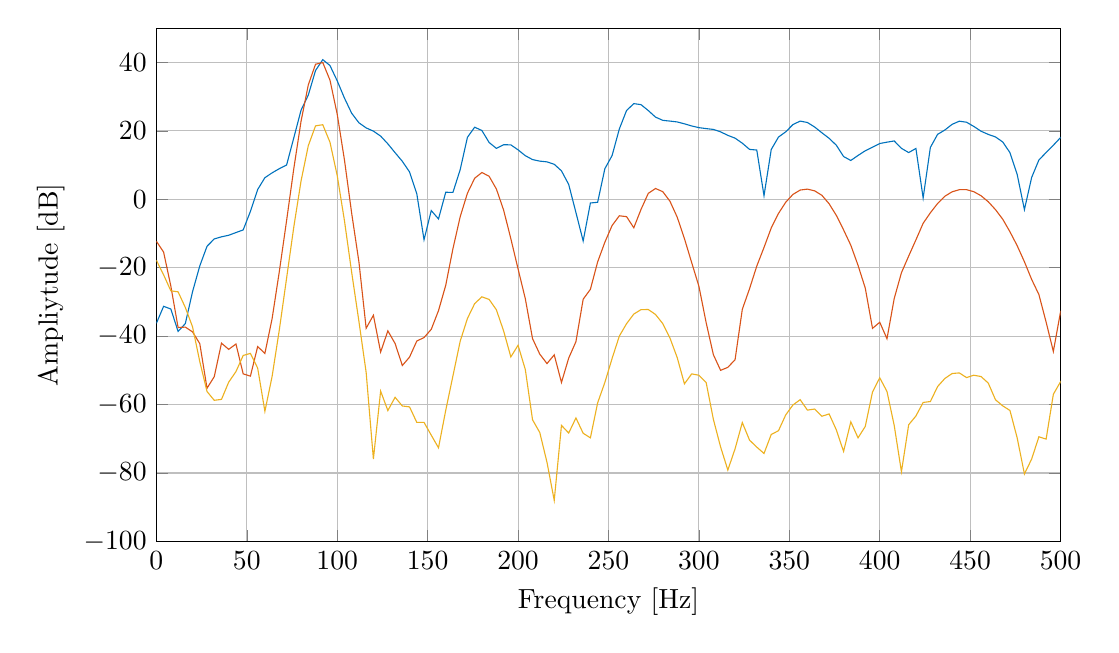
\begin{tikzpicture}

\begin{axis}[%
width=4.521in,
height=2.566in,
at={(0.758in,0.481in)},
scale only axis,
xmin=0,
xmax=500,
xmajorgrids,
ymin=-100,
ymax=50,
ymajorgrids,
xlabel = {Frequency [Hz]},
ylabel = {Ampliytude [dB]},
axis background/.style={fill=white}
]
\addplot [color=mycolor1,solid,forget plot]
  table[row sep=crcr]{%
0	-36.2456627243445\\
4	-31.2759458533165\\
8	-32.0776619775127\\
12	-38.6125202890656\\
16	-36.3345323053453\\
20	-27.0077369967815\\
24	-19.4693943957557\\
28	-13.732339490575\\
32	-11.5807317526438\\
36	-10.9690249691442\\
40	-10.511906993547\\
44	-9.72311303921483\\
48	-8.95211199801677\\
52	-3.53014873376706\\
56	2.84985902328302\\
60	6.32170668333729\\
64	7.73271925463987\\
68	8.95054418483462\\
72	10.0075228410197\\
76	17.9957316464693\\
80	26.045346441109\\
84	30.457626218315\\
88	37.6251571632718\\
92	40.8250217464457\\
96	39.0892035471452\\
100	34.6235828038179\\
104	29.5699447065432\\
108	25.1433887229802\\
112	22.3576097952116\\
116	20.8646916315058\\
120	19.9241336857616\\
124	18.472732341941\\
128	16.204733869856\\
132	13.6196437856485\\
136	11.1013075758865\\
140	7.99166996956162\\
144	1.62396141763164\\
148	-11.8325021373648\\
152	-3.2984151252917\\
156	-5.73668721552419\\
160	2.04711415216091\\
164	2.02985574714828\\
168	8.66924842595592\\
172	18.1109967276352\\
176	21.0704360488716\\
180	20.0996884934558\\
184	16.5965770793381\\
188	14.8930015958921\\
192	15.9524417173127\\
196	15.9057028453994\\
200	14.4547253745259\\
204	12.7449882390982\\
208	11.6056931798645\\
212	11.1535405767167\\
216	10.9390510372725\\
220	10.2310433623445\\
224	8.31476065218885\\
228	4.33545863764797\\
232	-3.87108845717101\\
236	-12.1973708256649\\
240	-1.08169197325651\\
244	-0.874129385856304\\
248	8.94722407260948\\
252	12.7880584999054\\
256	20.5591791800115\\
260	25.9584911846603\\
264	27.9622370372517\\
268	27.6617969197214\\
272	25.9392756536378\\
276	24.0244730781726\\
280	23.0790342884129\\
284	22.8542656462174\\
288	22.6098170894546\\
292	22.0551977243052\\
296	21.4339852432543\\
300	20.9399696925786\\
304	20.6588176126709\\
308	20.4172597744565\\
312	19.7096999527337\\
316	18.684999249698\\
320	17.8721463011533\\
324	16.3924700772466\\
328	14.5866497283843\\
332	14.3917030852375\\
336	1.04546311177496\\
340	14.5530347583429\\
344	18.1829634723254\\
348	19.7136995910232\\
352	21.8401013410047\\
356	22.8547097126057\\
360	22.4468301281197\\
364	21.1285418421379\\
368	19.4431405865107\\
372	17.8213836809138\\
376	15.7977782559822\\
380	12.501619530722\\
384	11.3438865208328\\
388	12.8145580776421\\
392	14.1864434948905\\
396	15.2409846881254\\
400	16.3030994444042\\
404	16.6961658238117\\
408	17.0470470203459\\
412	14.8918980400766\\
416	13.6536675260969\\
420	14.8561014366877\\
424	0.384482173036856\\
428	15.1638958212407\\
432	18.987997947683\\
436	20.245108759595\\
440	21.9016666282161\\
444	22.8265167327497\\
448	22.5224204374786\\
452	21.2931371643563\\
456	19.8996569112845\\
460	18.9651808292316\\
464	18.2280891967941\\
468	16.7551380819249\\
472	13.6385130887548\\
476	7.27369525785863\\
480	-3.01444057081381\\
484	6.38123995057743\\
488	11.4741119860737\\
492	13.6681310178868\\
496	15.8009494496232\\
500	18.0536609546208\\
504	15.3452017404259\\
};
\addplot [color=mycolor2,solid,forget plot]
  table[row sep=crcr]{%
0	-12.2520119318486\\
4	-15.457246347163\\
8	-25.3910173043042\\
12	-37.4725568579776\\
16	-37.3562445654259\\
20	-38.7562873098217\\
24	-42.1876755337237\\
28	-55.2230038989078\\
32	-51.8437687713913\\
36	-42.0532596081128\\
40	-43.8616126543261\\
44	-42.2946076259495\\
48	-51.0209190969441\\
52	-51.6880624037585\\
56	-43.0467675437237\\
60	-45.0414605676052\\
64	-34.8616871742125\\
68	-21.0560951260158\\
72	-6.22477934653492\\
76	9.01920930812603\\
80	22.8214255705148\\
84	33.4224041360244\\
88	39.4694493266955\\
92	39.9787288925826\\
96	34.8176671414911\\
100	24.863578028322\\
104	11.4873261064458\\
108	-4.11512257532409\\
112	-18.3006994856228\\
116	-37.6940669233946\\
120	-33.8883068315645\\
124	-44.6512198998014\\
128	-38.451189683929\\
132	-42.1493579806229\\
136	-48.5844637862039\\
140	-46.1225795980713\\
144	-41.4307693361984\\
148	-40.4105073069862\\
152	-38.0101945947228\\
156	-32.5425091605697\\
160	-25.1447891749562\\
164	-14.4049048926689\\
168	-5.09441327607532\\
172	1.78060576426878\\
176	6.15039756653658\\
180	7.82505796493828\\
184	6.72394606219921\\
188	3.02346566351573\\
192	-3.13070640987898\\
196	-11.5065028162916\\
200	-20.3568425006133\\
204	-29.0366851604597\\
208	-40.7128985278849\\
212	-45.2574360991406\\
216	-48.0175317037803\\
220	-45.4653377556674\\
224	-53.5338028069735\\
228	-46.424098969842\\
232	-41.6150076240414\\
236	-29.2127489596131\\
240	-26.3116395393023\\
244	-18.3124827937642\\
248	-12.5377778555752\\
252	-7.65752118724678\\
256	-4.82030346102452\\
260	-5.07544393128387\\
264	-8.32493945949036\\
268	-2.94762081977006\\
272	1.72178154534596\\
276	3.15551847796161\\
280	2.23430229797106\\
284	-0.579958561067868\\
288	-5.22070801896483\\
292	-11.488501776064\\
296	-18.4977907679757\\
300	-25.4236330689935\\
304	-36.0361296259341\\
308	-45.4229329097162\\
312	-49.9905971669865\\
316	-49.1257655730819\\
320	-46.8804009837873\\
324	-32.1573714025011\\
328	-26.1368574815249\\
332	-19.5256342068777\\
336	-14.0770872227808\\
340	-8.38129953507847\\
344	-4.14466167836757\\
348	-0.872890714687549\\
352	1.42538120503106\\
356	2.70197331240548\\
360	2.9706431978402\\
364	2.46731592419315\\
368	1.16029011129283\\
372	-1.30538261811383\\
376	-4.71639095206136\\
380	-8.94304674713556\\
384	-13.4301118262866\\
388	-19.3087033100694\\
392	-25.9673225742777\\
396	-37.7226046853454\\
400	-35.9447648931512\\
404	-40.7623704428332\\
408	-29.0089260880939\\
412	-21.4586761307658\\
416	-16.5981945929571\\
420	-11.8665589445147\\
424	-7.01866379220067\\
428	-3.94151038515161\\
432	-1.22430450029974\\
436	0.88960531056877\\
440	2.18459573963671\\
444	2.80465667399231\\
448	2.80771957803426\\
452	2.22737220051512\\
456	1.04249713097408\\
460	-0.718753360026654\\
464	-3.02144491943002\\
468	-5.81833646439779\\
472	-9.48808403450077\\
476	-13.5686247049238\\
480	-18.2514089125586\\
484	-23.4257046750688\\
488	-27.8333673151269\\
492	-35.8903151830065\\
496	-44.4761102433801\\
500	-32.8077200235739\\
504	-29.8452907639691\\
};
\addplot [color=mycolor3,solid,forget plot]
  table[row sep=crcr]{%
0	-17.8171623849573\\
4	-22.0871304556474\\
8	-26.7605950757654\\
12	-27.0473590664979\\
16	-31.6140519466276\\
20	-37.2923219172808\\
24	-47.4402911605021\\
28	-56.1895471107498\\
32	-58.7539992284481\\
36	-58.481721686763\\
40	-53.4407053671902\\
44	-50.3639645589143\\
48	-45.653292066664\\
52	-45.033471941546\\
56	-49.3334088914602\\
60	-61.9864928336348\\
64	-51.7396555138723\\
68	-38.0914465652888\\
72	-23.0692349827435\\
76	-8.04622680933582\\
80	5.370575787625\\
84	15.6625081498384\\
88	21.4585352100133\\
92	21.802476278155\\
96	16.6667244284307\\
100	6.92805941959042\\
104	-6.26733413099112\\
108	-21.391851018122\\
112	-35.6899317565\\
116	-50.6197727750267\\
120	-75.9172255179527\\
124	-56.0634402841978\\
128	-61.7508747618951\\
132	-57.8690629310526\\
136	-60.4110604874674\\
140	-60.6839879099036\\
144	-65.2129122668907\\
148	-65.1983597409115\\
152	-68.9547970093869\\
156	-72.6307278963048\\
160	-61.6907453362862\\
164	-51.5850082164483\\
168	-41.4741751381366\\
172	-34.8453736427206\\
176	-30.4916613216851\\
180	-28.5128369135712\\
184	-29.2711115887791\\
188	-32.2887931357218\\
192	-38.4602790192305\\
196	-46.0677094789475\\
200	-42.6696662867624\\
204	-49.7368953446889\\
208	-64.4452938008926\\
212	-68.1605799163304\\
216	-76.8829052489993\\
220	-88.0069185906183\\
224	-66.086657457663\\
228	-68.3191823061978\\
232	-63.9143735805713\\
236	-68.3867782915057\\
240	-69.7241329240411\\
244	-59.5093854684557\\
248	-53.5236219739806\\
252	-46.518637646594\\
256	-39.9835937493057\\
260	-36.3521020561078\\
264	-33.550944148426\\
268	-32.2424634700224\\
272	-32.2207242975908\\
276	-33.6608367553349\\
280	-36.3247560700635\\
284	-40.5601840074546\\
288	-46.2615693544122\\
292	-53.9473997491477\\
296	-51.0308492025798\\
300	-51.4260480650725\\
304	-53.5334880312033\\
308	-64.3125722299687\\
312	-72.3997520936646\\
316	-79.1355686260166\\
320	-72.9352062421103\\
324	-65.2576232966292\\
328	-70.3907922403966\\
332	-72.433258848779\\
336	-74.2918930111868\\
340	-68.7346087080537\\
344	-67.646314097029\\
348	-63.0313832944543\\
352	-60.1149343527707\\
356	-58.573068605131\\
360	-61.6167567025125\\
364	-61.3092912319025\\
368	-63.418442319508\\
372	-62.7361018074775\\
376	-67.3976044937552\\
380	-73.7062659524425\\
384	-65.0437032036963\\
388	-69.7210711588816\\
392	-66.3862663691021\\
396	-56.3221161578425\\
400	-52.1765755690186\\
404	-56.1687953461351\\
408	-66.0958334612276\\
412	-79.6326212226488\\
416	-65.9047091904128\\
420	-63.3360413847449\\
424	-59.3849489318673\\
428	-59.1091138578939\\
432	-54.7217548502314\\
436	-52.3839258562663\\
440	-50.9277593354018\\
444	-50.7464587091174\\
448	-52.111703667707\\
452	-51.42413181944\\
456	-51.8077131156495\\
460	-53.713560851602\\
464	-58.5957179358222\\
468	-60.3717718602905\\
472	-61.719843878435\\
476	-69.7360582460514\\
480	-80.2872255947469\\
484	-75.928207578822\\
488	-69.4186253438429\\
492	-70.0929450696748\\
496	-56.9930897356615\\
500	-53.3123095796073\\
504	-57.5347032563323\\
};
\end{axis}
\end{tikzpicture}%
\caption{The spectrum of the window. The yellow graph is dataset 1, red is 10 and blue is 19.}
\label{fig:FFT_hit}
\end{figure}

It is seen that the energy for non-harmonic frequencies is increased at very low frequencies as indicated with the arrow. The yellow graph is the first dataset and the red is the tenth dataset. As no hit was observed in the window at dataset 1 and 10, the energy of lower part of the spectrum was not increased. However the suspected hit in dataset 19 has an energy increase in the low frequency spectrum. Note that since the window is 0.25 seconds wide, frequencies below 4 Hz should be discarded.

\section{Error sources}

Few errors could have occurred during trials, since then only variable adjusted during between measurements were the gain of the amplifier. There were however problems with moving the setup from the control room were it was calibrated and then moved into the anechoic room. The calibration was done using an visual equalizer where the output was shown with a bar chart Hence the data should bee seen with a tolerance of +/- 0.5 dB.